\documentclass[a4paper]{book}
\usepackage{makeidx}
\usepackage{graphicx}
\usepackage{multicol}
\usepackage{float}
\usepackage{listings}
\usepackage{color}
\usepackage{ifthen}
\usepackage[table]{xcolor}
\usepackage{textcomp}
\usepackage{alltt}
\usepackage{ifpdf}
\ifpdf
\usepackage[pdftex,
            pagebackref=true,
            colorlinks=true,
            linkcolor=blue,
            unicode
           ]{hyperref}
\else
\usepackage[ps2pdf,
            pagebackref=true,
            colorlinks=true,
            linkcolor=blue,
            unicode
           ]{hyperref}
\usepackage{pspicture}
\fi
\usepackage[utf8]{inputenc}
\usepackage{mathptmx}
\usepackage[scaled=.90]{helvet}
\usepackage{courier}
\usepackage{sectsty}
\usepackage[titles]{tocloft}
\usepackage{doxygen}
\lstset{language=C++,inputencoding=utf8,basicstyle=\footnotesize,breaklines=true,breakatwhitespace=true,tabsize=8,numbers=left }
\makeindex
\setcounter{tocdepth}{3}
\renewcommand{\footrulewidth}{0.4pt}
\renewcommand{\familydefault}{\sfdefault}
\begin{document}
\hypersetup{pageanchor=false}
\begin{titlepage}
\vspace*{7cm}
\begin{center}
{\Large EPICS QT Framework \\[1ex]\large 2.5.0 }\\
\vspace*{1cm}
{\large Generated by Doxygen 1.7.4}\\
\vspace*{0.5cm}
{\small Tue Jun 4 2013 15:06:38}\\
\end{center}
\end{titlepage}
\clearemptydoublepage
\pagenumbering{roman}
\tableofcontents
\clearemptydoublepage
\pagenumbering{arabic}
\hypersetup{pageanchor=true}
\chapter{QE framework -\/ EPICS aware Qt Widgets and data access classes}
\label{index}\hypertarget{index}{}
\begin{DoxyItemize}
\item QE is a layered software framework for accessing EPICS data using Channel Access on a range of platforms.\par
\par

\end{DoxyItemize}


\begin{DoxyItemize}
\item The QE framework provides object oriented C++ access to control systems using EPICS (Experimental Physics and Industrial Control System). It is based on Qt, a widely used cross-\/platform application development framework.\par
\par

\end{DoxyItemize}


\begin{DoxyItemize}
\item GUI or console based applications can be written that use QE at several levels. QE includes Qt plugin libraries, EPICS aware widgets, data formatting classes, and classes for accessing raw EPICS data in a Qt friendly way.\par
\par

\end{DoxyItemize}


\begin{DoxyItemize}
\item QE also includes an application -\/ QEgui -\/ for displaying forms produced by the Qt development tool ‘Designer’. Using this application a complete EPICS GUI system can be generated without writing any code. A GUI system produced in this way can interact with existing EPICS display tools such as EDM.\par
\par

\end{DoxyItemize}


\begin{DoxyItemize}
\item QE handles much of the complexities of Channel Access including initiating and managing a channel. Applications using QE can interact with Channel Access using Qt based classes and data types. Channel Access updates are delivered using Qt’s signals and slots mechanism.
\end{DoxyItemize}

\hypertarget{index_documentation}{}\section{Documentation}\label{index_documentation}
Support documents can be found in the \href{https://sourceforge.net/projects/epicsqt/files/documentation/}{\tt documentation} section of the epicsqt sourceforge project. The framework download (available on the epicsqt sourceforge \href{https://sourceforge.net/projects/epicsqt/}{\tt homepage}) also includes this documentation as well as full Doxygen generated documentation of all the epicsqt classes and widgets.\hypertarget{index_license}{}\section{License}\label{index_license}
epicsqt is distributed under the terms of the \hyperlink{epicsqtlicense}{GNU General Public License}.\hypertarget{index_platforms}{}\section{Platforms}\label{index_platforms}
epicsqt might be usable in all environments where you find \href{http://www.trolltech.com/products/qt}{\tt Qt}. It is compatible with Qt $>$= 4.4.\hypertarget{index_screenshotsonmainpage}{}\section{Screenshots}\label{index_screenshotsonmainpage}

\begin{DoxyItemize}
\item \hyperlink{ASguiscreenshots}{ASgui screen shots}\par

\item \hyperlink{otherappscreenshots}{other applications using epicsqt widgets}\par

\item \hyperlink{designerscreenshots}{Qt Designer}\par

\item \hyperlink{qtcreatorscreenshots}{Qt Creator}\par

\end{DoxyItemize}

 Screenshots are only available in the HTML docs.\hypertarget{index_downloads}{}\section{Downloads}\label{index_downloads}
Stable releases and development snapshots are available at the epicsqt \href{http://sourceforge.net/projects/epicsqt}{\tt project page}.

For getting a development snapshot from the SVN repository: 
\begin{DoxyCode}
 svn svn co https://epicsqt.svn.sourceforge.net/svnroot/epicsqt epicsqt
\end{DoxyCode}


Alternativly, get a packaged file (epicsqt.tar.gz) from the \href{http://epicsqt.svn.sourceforge.net/viewvc/epicsqt/?view=tar}{\tt epicsqt repository site}.\hypertarget{index_installonmainpage}{}\section{Installation}\label{index_installonmainpage}
Read \href{http://sourceforge.net/projects/epicsqt/files/documentation/QE_GettingStarted.pdf/download}{\tt QE\_\-GettingStarted.pdf} in the documentation for setting up an enviroment for building or using the epicsqt framework.\par
 To build the framework, open epicsqt.pro in QtCreator, ensure shaddow build is turned off, and hit build.\par
 The resultant library libQEPlugin.so will need to be installed or referenced up according to how it is to be used -\/ see QE\_\-GettingStarted.pdf for details.\par
 Any Qt specific queries? start at \href{http://qt-project.org}{\tt the Qt Project}\hypertarget{index_support}{}\section{Support}\label{index_support}
Visit the sourceforge epicsqt \href{http://sourceforge.net/projects/epicsqt/support}{\tt support page} for assistance.\hypertarget{index_relatedprojects}{}\section{Related Projects}\label{index_relatedprojects}
\href{http://qwt.sourceforge.net/}{\tt Qwt}, The core of a Channel Access aware plotting widget.\hypertarget{index_credits}{}\section{Credits:}\label{index_credits}
\begin{DoxyParagraph}{Authors: }
Andrew Rhyder, Anthony Owen, Glenn Jackson 
\end{DoxyParagraph}
\begin{DoxyParagraph}{Project admin:}
Andrew Rhyder $<$\href{mailto:andrew.rhyder@synchrotron.org.au}{\tt andrew.rhyder@synchrotron.org.au}$>$ 
\end{DoxyParagraph}

\chapter{GNU General Public License}
\label{epicsqtlicense}
\hypertarget{epicsqtlicense}{}
\input{epicsqtlicense}
\chapter{ASgui screen shots}
\label{ASguiscreenshots}
\hypertarget{ASguiscreenshots}{}
 
\begin{DoxyImage}
\includegraphics[width=12cm]{ASguiExample1}
\caption{Australian Synchrotron mock up}
\end{DoxyImage}
 \par
\par


 \par
\par
 
\begin{DoxyImage}
\includegraphics[width=12cm]{ASguiExample2}
\caption{Monochromator referencing}
\end{DoxyImage}
 \par
\par


 
\begin{DoxyImage}
\includegraphics[width=12cm]{ASguiExample3}
\caption{Beam position monitor}
\end{DoxyImage}
 \par
\par


 
\begin{DoxyImage}
\includegraphics[width=12cm]{ASguiExample4}
\caption{Insertion device}
\end{DoxyImage}
 \par
\par


 
\begin{DoxyImage}
\includegraphics[width=12cm]{ASguiExample5}
\caption{Injection efficiency monitor}
\end{DoxyImage}
 
\chapter{other applications using epicsqt widgets}
\label{otherappscreenshots}
\hypertarget{otherappscreenshots}{}
 
\begin{DoxyImage}
\includegraphics[width=12cm]{otherappExample1}
\caption{Medical Imaging beamline}
\end{DoxyImage}
 \par
\par


 
\begin{DoxyImage}
\includegraphics[width=12cm]{otherappExample2}
\caption{Motor controller}
\end{DoxyImage}
 \par
\par


 
\begin{DoxyImage}
\includegraphics[width=12cm]{otherappExample3}
\caption{Motor controller}
\end{DoxyImage}
 
\chapter{Qt Designer}
\label{designerscreenshots}
\hypertarget{designerscreenshots}{}
 
\begin{DoxyImage}
\includegraphics[width=12cm]{designerExample1}
\caption{Editing multiple GUIs}
\end{DoxyImage}
 \par
\par


 
\begin{DoxyImage}
\includegraphics[width=12cm]{designerExample2}
\caption{Editing a GUI}
\end{DoxyImage}
 
\chapter{Qt Creator}
\label{qtcreatorscreenshots}
\hypertarget{qtcreatorscreenshots}{}
 
\begin{DoxyImage}
\includegraphics[width=12cm]{qtcreatorExample1}
\caption{Application using epicsqt data source classes}
\end{DoxyImage}
 
\chapter{Class Index}
\section{Class Hierarchy}
This inheritance list is sorted roughly, but not completely, alphabetically:\begin{DoxyCompactList}
\item \contentsline{section}{\_\-Field}{\pageref{class__Field}}{}
\item \contentsline{section}{\_\-Item}{\pageref{class__Item}}{}
\item \contentsline{section}{\_\-QDialogItem}{\pageref{class__QDialogItem}}{}
\item \contentsline{section}{\_\-QDialogLogin}{\pageref{class__QDialogLogin}}{}
\item \contentsline{section}{\_\-QPushButtonGroup}{\pageref{class__QPushButtonGroup}}{}
\item \contentsline{section}{\_\-QTableWidgetFileBrowser}{\pageref{class__QTableWidgetFileBrowser}}{}
\item \contentsline{section}{\_\-QTableWidgetLog}{\pageref{class__QTableWidgetLog}}{}
\item \contentsline{section}{\_\-QTableWidgetScript}{\pageref{class__QTableWidgetScript}}{}
\item \contentsline{section}{QEAnalogIndicator::Band}{\pageref{structQEAnalogIndicator_1_1Band}}{}
\item \contentsline{section}{QEAnalogIndicator::BandList}{\pageref{classQEAnalogIndicator_1_1BandList}}{}
\item \contentsline{section}{ChartState}{\pageref{classChartState}}{}
\item \contentsline{section}{ContainerProfile}{\pageref{classContainerProfile}}{}
\begin{DoxyCompactList}
\item \contentsline{section}{QEWidget}{\pageref{classQEWidget}}{}
\begin{DoxyCompactList}
\item \contentsline{section}{QEAnalogProgressBar}{\pageref{classQEAnalogProgressBar}}{}
\item \contentsline{section}{QEBitStatus}{\pageref{classQEBitStatus}}{}
\item \contentsline{section}{QEComboBox}{\pageref{classQEComboBox}}{}
\item \contentsline{section}{QEConfiguredLayout}{\pageref{classQEConfiguredLayout}}{}
\item \contentsline{section}{QEFileBrowser}{\pageref{classQEFileBrowser}}{}
\item \contentsline{section}{QEForm}{\pageref{classQEForm}}{}
\item \contentsline{section}{QEFrame}{\pageref{classQEFrame}}{}
\item \contentsline{section}{QEGenericButton}{\pageref{classQEGenericButton}}{}
\begin{DoxyCompactList}
\item \contentsline{section}{QECheckBox}{\pageref{classQECheckBox}}{}
\item \contentsline{section}{QEPushButton}{\pageref{classQEPushButton}}{}
\item \contentsline{section}{QERadioButton}{\pageref{classQERadioButton}}{}
\end{DoxyCompactList}
\item \contentsline{section}{QEGenericEdit}{\pageref{classQEGenericEdit}}{}
\begin{DoxyCompactList}
\item \contentsline{section}{QELineEdit}{\pageref{classQELineEdit}}{}
\item \contentsline{section}{QENumericEdit}{\pageref{classQENumericEdit}}{}
\end{DoxyCompactList}
\item \contentsline{section}{QEGroupBox}{\pageref{classQEGroupBox}}{}
\item \contentsline{section}{QEImage}{\pageref{classQEImage}}{}
\item \contentsline{section}{QELabel}{\pageref{classQELabel}}{}
\item \contentsline{section}{QELink}{\pageref{classQELink}}{}
\item \contentsline{section}{QELog}{\pageref{classQELog}}{}
\item \contentsline{section}{QELogin}{\pageref{classQELogin}}{}
\item \contentsline{section}{QEPeriodic}{\pageref{classQEPeriodic}}{}
\item \contentsline{section}{QEPlot}{\pageref{classQEPlot}}{}
\item \contentsline{section}{QEPvProperties}{\pageref{classQEPvProperties}}{}
\item \contentsline{section}{QERecipe}{\pageref{classQERecipe}}{}
\item \contentsline{section}{QEScript}{\pageref{classQEScript}}{}
\item \contentsline{section}{QEShape}{\pageref{classQEShape}}{}
\item \contentsline{section}{QESlider}{\pageref{classQESlider}}{}
\item \contentsline{section}{QESpinBox}{\pageref{classQESpinBox}}{}
\item \contentsline{section}{QEStripChart}{\pageref{classQEStripChart}}{}
\item \contentsline{section}{QESubstitutedLabel}{\pageref{classQESubstitutedLabel}}{}
\end{DoxyCompactList}
\end{DoxyCompactList}
\item \contentsline{section}{contextMenu}{\pageref{classcontextMenu}}{}
\begin{DoxyCompactList}
\item \contentsline{section}{QEWidget}{\pageref{classQEWidget}}{}
\end{DoxyCompactList}
\item \contentsline{section}{contextMenuObject}{\pageref{classcontextMenuObject}}{}
\item \contentsline{section}{QEPeriodic::elementInfoStruct}{\pageref{structQEPeriodic_1_1elementInfoStruct}}{}
\item \contentsline{section}{flipRotateMenu}{\pageref{classflipRotateMenu}}{}
\item \contentsline{section}{imageContextMenu}{\pageref{classimageContextMenu}}{}
\item \contentsline{section}{imageInfo}{\pageref{classimageInfo}}{}
\begin{DoxyCompactList}
\item \contentsline{section}{QEImage}{\pageref{classQEImage}}{}
\end{DoxyCompactList}
\item \contentsline{section}{imageMarkup}{\pageref{classimageMarkup}}{}
\begin{DoxyCompactList}
\item \contentsline{section}{VideoWidget}{\pageref{classVideoWidget}}{}
\end{DoxyCompactList}
\item \contentsline{section}{managePixmaps}{\pageref{classmanagePixmaps}}{}
\begin{DoxyCompactList}
\item \contentsline{section}{QEGenericButton}{\pageref{classQEGenericButton}}{}
\item \contentsline{section}{QELabel}{\pageref{classQELabel}}{}
\end{DoxyCompactList}
\item \contentsline{section}{markupItem}{\pageref{classmarkupItem}}{}
\begin{DoxyCompactList}
\item \contentsline{section}{markupBeam}{\pageref{classmarkupBeam}}{}
\item \contentsline{section}{markupHLine}{\pageref{classmarkupHLine}}{}
\item \contentsline{section}{markupLine}{\pageref{classmarkupLine}}{}
\item \contentsline{section}{markupRegion}{\pageref{classmarkupRegion}}{}
\item \contentsline{section}{markupTarget}{\pageref{classmarkupTarget}}{}
\item \contentsline{section}{markupText}{\pageref{classmarkupText}}{}
\item \contentsline{section}{markupVLine}{\pageref{classmarkupVLine}}{}
\end{DoxyCompactList}
\item \contentsline{section}{message\_\-types}{\pageref{classmessage__types}}{}
\item \contentsline{section}{QEStripChartToolBar::OwnWidgets}{\pageref{classQEStripChartToolBar_1_1OwnWidgets}}{}
\item \contentsline{section}{QEPvProperties::OwnWidgets}{\pageref{classQEPvProperties_1_1OwnWidgets}}{}
\item \contentsline{section}{PeriodicDialog}{\pageref{classPeriodicDialog}}{}
\item \contentsline{section}{PeriodicElementSetupForm}{\pageref{classPeriodicElementSetupForm}}{}
\item \contentsline{section}{PeriodicSetupDialog}{\pageref{classPeriodicSetupDialog}}{}
\item \contentsline{section}{PersistanceManager}{\pageref{classPersistanceManager}}{}
\item \contentsline{section}{PMContext}{\pageref{classPMContext}}{}
\item \contentsline{section}{PMElement}{\pageref{classPMElement}}{}
\item \contentsline{section}{PMElementList}{\pageref{classPMElementList}}{}
\item \contentsline{section}{QEStripChart::PrivateData}{\pageref{classQEStripChart_1_1PrivateData}}{}
\item \contentsline{section}{QEStripChartItem::PrivateData}{\pageref{classQEStripChartItem_1_1PrivateData}}{}
\item \contentsline{section}{profilePlot}{\pageref{classprofilePlot}}{}
\item \contentsline{section}{PublishedProfile}{\pageref{classPublishedProfile}}{}
\item \contentsline{section}{PushButtonSpecifications}{\pageref{structPushButtonSpecifications}}{}
\item \contentsline{section}{QBitStatus}{\pageref{classQBitStatus}}{}
\begin{DoxyCompactList}
\item \contentsline{section}{QEBitStatus}{\pageref{classQEBitStatus}}{}
\end{DoxyCompactList}
\item \contentsline{section}{QCaAlarmInfo}{\pageref{classQCaAlarmInfo}}{}
\item \contentsline{section}{QCaConnectionInfo}{\pageref{classQCaConnectionInfo}}{}
\item \contentsline{section}{QCaDataPoint}{\pageref{structQCaDataPoint}}{}
\item \contentsline{section}{QCaDataPointList}{\pageref{classQCaDataPointList}}{}
\item \contentsline{section}{QCaDateTime}{\pageref{classQCaDateTime}}{}
\item \contentsline{section}{QCaEventFilter}{\pageref{classQCaEventFilter}}{}
\item \contentsline{section}{QCaEventItem}{\pageref{classQCaEventItem}}{}
\item \contentsline{section}{QCaEventUpdate}{\pageref{classQCaEventUpdate}}{}
\item \contentsline{section}{QCaInstalledFiltersListItem}{\pageref{classQCaInstalledFiltersListItem}}{}
\item \contentsline{section}{qcaobject::QCaObject}{\pageref{classqcaobject_1_1QCaObject}}{}
\begin{DoxyCompactList}
\item \contentsline{section}{QEByteArray}{\pageref{classQEByteArray}}{}
\item \contentsline{section}{QEFloating}{\pageref{classQEFloating}}{}
\item \contentsline{section}{QEInteger}{\pageref{classQEInteger}}{}
\item \contentsline{section}{QEString}{\pageref{classQEString}}{}
\end{DoxyCompactList}
\item \contentsline{section}{QCaVariableNamePropertyManager}{\pageref{classQCaVariableNamePropertyManager}}{}
\item \contentsline{section}{QEAnalogIndicator}{\pageref{classQEAnalogIndicator}}{}
\begin{DoxyCompactList}
\item \contentsline{section}{QEAnalogProgressBar}{\pageref{classQEAnalogProgressBar}}{}
\end{DoxyCompactList}
\item \contentsline{section}{QEChartStateLists}{\pageref{classQEChartStateLists}}{}
\item \contentsline{section}{QECheckBoxManager}{\pageref{classQECheckBoxManager}}{}
\item \contentsline{section}{QEConfiguredLayoutManager}{\pageref{classQEConfiguredLayoutManager}}{}
\item \contentsline{section}{QEDragDrop}{\pageref{classQEDragDrop}}{}
\begin{DoxyCompactList}
\item \contentsline{section}{QEWidget}{\pageref{classQEWidget}}{}
\end{DoxyCompactList}
\item \contentsline{section}{QEFloatingFormatting}{\pageref{classQEFloatingFormatting}}{}
\item \contentsline{section}{QEIntegerFormatting}{\pageref{classQEIntegerFormatting}}{}
\item \contentsline{section}{QELineEditManager}{\pageref{classQELineEditManager}}{}
\item \contentsline{section}{QELocalEnumeration}{\pageref{classQELocalEnumeration}}{}
\item \contentsline{section}{QENumericEditManager}{\pageref{classQENumericEditManager}}{}
\item \contentsline{section}{QEPeriodicComponentData}{\pageref{classQEPeriodicComponentData}}{}
\item \contentsline{section}{QEPeriodicTaskMenu}{\pageref{classQEPeriodicTaskMenu}}{}
\item \contentsline{section}{QEPeriodicTaskMenuFactory}{\pageref{classQEPeriodicTaskMenuFactory}}{}
\item \contentsline{section}{QEpicsPV}{\pageref{classQEpicsPV}}{}
\item \contentsline{section}{QEPVNameLists}{\pageref{classQEPVNameLists}}{}
\item \contentsline{section}{QEPvPropertiesManager}{\pageref{classQEPvPropertiesManager}}{}
\item \contentsline{section}{QERecordFieldName}{\pageref{classQERecordFieldName}}{}
\item \contentsline{section}{QERecordSpec}{\pageref{classQERecordSpec}}{}
\item \contentsline{section}{QERecordSpecList}{\pageref{classQERecordSpecList}}{}
\item \contentsline{section}{QEStringFormatting}{\pageref{classQEStringFormatting}}{}
\item \contentsline{section}{QEStringFormattingMethods}{\pageref{classQEStringFormattingMethods}}{}
\begin{DoxyCompactList}
\item \contentsline{section}{QEAnalogProgressBar}{\pageref{classQEAnalogProgressBar}}{}
\item \contentsline{section}{QEGenericButton}{\pageref{classQEGenericButton}}{}
\item \contentsline{section}{QELabel}{\pageref{classQELabel}}{}
\item \contentsline{section}{QELineEdit}{\pageref{classQELineEdit}}{}
\end{DoxyCompactList}
\item \contentsline{section}{QEStripChartAdjustPVDialog}{\pageref{classQEStripChartAdjustPVDialog}}{}
\item \contentsline{section}{QEStripChartContextMenu}{\pageref{classQEStripChartContextMenu}}{}
\item \contentsline{section}{QEStripChartItem}{\pageref{classQEStripChartItem}}{}
\item \contentsline{section}{QEStripChartItemDialog}{\pageref{classQEStripChartItemDialog}}{}
\item \contentsline{section}{QEStripChartNames}{\pageref{classQEStripChartNames}}{}
\item \contentsline{section}{QEStripChartRangeDialog}{\pageref{classQEStripChartRangeDialog}}{}
\item \contentsline{section}{QEStripChartTimeDialog}{\pageref{classQEStripChartTimeDialog}}{}
\item \contentsline{section}{QEStripChartToolBar}{\pageref{classQEStripChartToolBar}}{}
\item \contentsline{section}{QEToolTip}{\pageref{classQEToolTip}}{}
\begin{DoxyCompactList}
\item \contentsline{section}{QEWidget}{\pageref{classQEWidget}}{}
\end{DoxyCompactList}
\item \contentsline{section}{QEWidgets}{\pageref{classQEWidgets}}{}
\item \contentsline{section}{QLabelList}{\pageref{classQLabelList}}{}
\item \contentsline{section}{ROIinfo}{\pageref{classROIinfo}}{}
\item \contentsline{section}{SaveRestoreSignal}{\pageref{classSaveRestoreSignal}}{}
\item \contentsline{section}{saveRestoreSlot}{\pageref{classsaveRestoreSlot}}{}
\item \contentsline{section}{selectMenu}{\pageref{classselectMenu}}{}
\item \contentsline{section}{standardProperties}{\pageref{classstandardProperties}}{}
\begin{DoxyCompactList}
\item \contentsline{section}{QEWidget}{\pageref{classQEWidget}}{}
\end{DoxyCompactList}
\item \contentsline{section}{StateMachineTemplate}{\pageref{classStateMachineTemplate}}{}
\begin{DoxyCompactList}
\item \contentsline{section}{qcastatemachine::QCaStateMachine}{\pageref{classqcastatemachine_1_1QCaStateMachine}}{}
\begin{DoxyCompactList}
\item \contentsline{section}{qcastatemachine::ConnectionQCaStateMachine}{\pageref{classqcastatemachine_1_1ConnectionQCaStateMachine}}{}
\item \contentsline{section}{qcastatemachine::ReadQCaStateMachine}{\pageref{classqcastatemachine_1_1ReadQCaStateMachine}}{}
\item \contentsline{section}{qcastatemachine::SubscriptionQCaStateMachine}{\pageref{classqcastatemachine_1_1SubscriptionQCaStateMachine}}{}
\item \contentsline{section}{qcastatemachine::WriteQCaStateMachine}{\pageref{classqcastatemachine_1_1WriteQCaStateMachine}}{}
\end{DoxyCompactList}
\end{DoxyCompactList}
\item \contentsline{section}{trace}{\pageref{classtrace}}{}
\item \contentsline{section}{TrackRange}{\pageref{classTrackRange}}{}
\item \contentsline{section}{userInfoStruct}{\pageref{classuserInfoStruct}}{}
\item \contentsline{section}{QEPeriodic::userInfoStructArray}{\pageref{structQEPeriodic_1_1userInfoStructArray}}{}
\item \contentsline{section}{userLevelSignal}{\pageref{classuserLevelSignal}}{}
\item \contentsline{section}{userLevelSlot}{\pageref{classuserLevelSlot}}{}
\item \contentsline{section}{userLevelTypes}{\pageref{classuserLevelTypes}}{}
\item \contentsline{section}{UserMessage}{\pageref{classUserMessage}}{}
\begin{DoxyCompactList}
\item \contentsline{section}{QEWidget}{\pageref{classQEWidget}}{}
\end{DoxyCompactList}
\item \contentsline{section}{UserMessageSignal}{\pageref{classUserMessageSignal}}{}
\item \contentsline{section}{UserMessageSlot}{\pageref{classUserMessageSlot}}{}
\item \contentsline{section}{ValueScaling}{\pageref{classValueScaling}}{}
\item \contentsline{section}{WidgetRef}{\pageref{classWidgetRef}}{}
\item \contentsline{section}{zoomMenu}{\pageref{classzoomMenu}}{}
\end{DoxyCompactList}

\chapter{Class Index}
\section{Class List}
Here are the classes, structs, unions and interfaces with brief descriptions:\begin{DoxyCompactList}
\item\contentsline{section}{\hyperlink{class__Field}{\_\-Field} }{\pageref{class__Field}}{}
\item\contentsline{section}{\hyperlink{class__Item}{\_\-Item} }{\pageref{class__Item}}{}
\item\contentsline{section}{\hyperlink{class__QDialogItem}{\_\-QDialogItem} }{\pageref{class__QDialogItem}}{}
\item\contentsline{section}{\hyperlink{class__QDialogLogin}{\_\-QDialogLogin} }{\pageref{class__QDialogLogin}}{}
\item\contentsline{section}{\hyperlink{class__QPushButtonGroup}{\_\-QPushButtonGroup} }{\pageref{class__QPushButtonGroup}}{}
\item\contentsline{section}{\hyperlink{class__QTableWidgetFileBrowser}{\_\-QTableWidgetFileBrowser} }{\pageref{class__QTableWidgetFileBrowser}}{}
\item\contentsline{section}{\hyperlink{class__QTableWidgetLog}{\_\-QTableWidgetLog} }{\pageref{class__QTableWidgetLog}}{}
\item\contentsline{section}{\hyperlink{class__QTableWidgetScript}{\_\-QTableWidgetScript} }{\pageref{class__QTableWidgetScript}}{}
\item\contentsline{section}{\hyperlink{structQEAnalogIndicator_1_1Band}{QEAnalogIndicator::Band} }{\pageref{structQEAnalogIndicator_1_1Band}}{}
\item\contentsline{section}{\hyperlink{classQEAnalogIndicator_1_1BandList}{QEAnalogIndicator::BandList} }{\pageref{classQEAnalogIndicator_1_1BandList}}{}
\item\contentsline{section}{\hyperlink{classChartState}{ChartState} }{\pageref{classChartState}}{}
\item\contentsline{section}{\hyperlink{classqcastatemachine_1_1ConnectionQCaStateMachine}{qcastatemachine::ConnectionQCaStateMachine} }{\pageref{classqcastatemachine_1_1ConnectionQCaStateMachine}}{}
\item\contentsline{section}{\hyperlink{classContainerProfile}{ContainerProfile} }{\pageref{classContainerProfile}}{}
\item\contentsline{section}{\hyperlink{classcontextMenu}{contextMenu} }{\pageref{classcontextMenu}}{}
\item\contentsline{section}{\hyperlink{classcontextMenuObject}{contextMenuObject} }{\pageref{classcontextMenuObject}}{}
\item\contentsline{section}{\hyperlink{structQEPeriodic_1_1elementInfoStruct}{QEPeriodic::elementInfoStruct} }{\pageref{structQEPeriodic_1_1elementInfoStruct}}{}
\item\contentsline{section}{\hyperlink{classflipRotateMenu}{flipRotateMenu} }{\pageref{classflipRotateMenu}}{}
\item\contentsline{section}{\hyperlink{classimageContextMenu}{imageContextMenu} }{\pageref{classimageContextMenu}}{}
\item\contentsline{section}{\hyperlink{classimageInfo}{imageInfo} }{\pageref{classimageInfo}}{}
\item\contentsline{section}{\hyperlink{classimageMarkup}{imageMarkup} }{\pageref{classimageMarkup}}{}
\item\contentsline{section}{\hyperlink{classmanagePixmaps}{managePixmaps} }{\pageref{classmanagePixmaps}}{}
\item\contentsline{section}{\hyperlink{classmarkupBeam}{markupBeam} }{\pageref{classmarkupBeam}}{}
\item\contentsline{section}{\hyperlink{classmarkupHLine}{markupHLine} }{\pageref{classmarkupHLine}}{}
\item\contentsline{section}{\hyperlink{classmarkupItem}{markupItem} }{\pageref{classmarkupItem}}{}
\item\contentsline{section}{\hyperlink{classmarkupLine}{markupLine} }{\pageref{classmarkupLine}}{}
\item\contentsline{section}{\hyperlink{classmarkupRegion}{markupRegion} }{\pageref{classmarkupRegion}}{}
\item\contentsline{section}{\hyperlink{classmarkupTarget}{markupTarget} }{\pageref{classmarkupTarget}}{}
\item\contentsline{section}{\hyperlink{classmarkupText}{markupText} }{\pageref{classmarkupText}}{}
\item\contentsline{section}{\hyperlink{classmarkupVLine}{markupVLine} }{\pageref{classmarkupVLine}}{}
\item\contentsline{section}{\hyperlink{classmessage__types}{message\_\-types} }{\pageref{classmessage__types}}{}
\item\contentsline{section}{\hyperlink{classQEStripChartToolBar_1_1OwnWidgets}{QEStripChartToolBar::OwnWidgets} }{\pageref{classQEStripChartToolBar_1_1OwnWidgets}}{}
\item\contentsline{section}{\hyperlink{classQEPvProperties_1_1OwnWidgets}{QEPvProperties::OwnWidgets} }{\pageref{classQEPvProperties_1_1OwnWidgets}}{}
\item\contentsline{section}{\hyperlink{classPeriodicDialog}{PeriodicDialog} }{\pageref{classPeriodicDialog}}{}
\item\contentsline{section}{\hyperlink{classPeriodicElementSetupForm}{PeriodicElementSetupForm} }{\pageref{classPeriodicElementSetupForm}}{}
\item\contentsline{section}{\hyperlink{classPeriodicSetupDialog}{PeriodicSetupDialog} }{\pageref{classPeriodicSetupDialog}}{}
\item\contentsline{section}{\hyperlink{classPersistanceManager}{PersistanceManager} }{\pageref{classPersistanceManager}}{}
\item\contentsline{section}{\hyperlink{classPMContext}{PMContext} }{\pageref{classPMContext}}{}
\item\contentsline{section}{\hyperlink{classPMElement}{PMElement} }{\pageref{classPMElement}}{}
\item\contentsline{section}{\hyperlink{classPMElementList}{PMElementList} }{\pageref{classPMElementList}}{}
\item\contentsline{section}{\hyperlink{classQEStripChart_1_1PrivateData}{QEStripChart::PrivateData} }{\pageref{classQEStripChart_1_1PrivateData}}{}
\item\contentsline{section}{\hyperlink{classQEStripChartItem_1_1PrivateData}{QEStripChartItem::PrivateData} }{\pageref{classQEStripChartItem_1_1PrivateData}}{}
\item\contentsline{section}{\hyperlink{classprofilePlot}{profilePlot} }{\pageref{classprofilePlot}}{}
\item\contentsline{section}{\hyperlink{classPublishedProfile}{PublishedProfile} }{\pageref{classPublishedProfile}}{}
\item\contentsline{section}{\hyperlink{structPushButtonSpecifications}{PushButtonSpecifications} }{\pageref{structPushButtonSpecifications}}{}
\item\contentsline{section}{\hyperlink{classQBitStatus}{QBitStatus} }{\pageref{classQBitStatus}}{}
\item\contentsline{section}{\hyperlink{classQCaAlarmInfo}{QCaAlarmInfo} }{\pageref{classQCaAlarmInfo}}{}
\item\contentsline{section}{\hyperlink{classQCaConnectionInfo}{QCaConnectionInfo} }{\pageref{classQCaConnectionInfo}}{}
\item\contentsline{section}{\hyperlink{structQCaDataPoint}{QCaDataPoint} }{\pageref{structQCaDataPoint}}{}
\item\contentsline{section}{\hyperlink{classQCaDataPointList}{QCaDataPointList} }{\pageref{classQCaDataPointList}}{}
\item\contentsline{section}{\hyperlink{classQCaDateTime}{QCaDateTime} }{\pageref{classQCaDateTime}}{}
\item\contentsline{section}{\hyperlink{classQCaEventFilter}{QCaEventFilter} }{\pageref{classQCaEventFilter}}{}
\item\contentsline{section}{\hyperlink{classQCaEventItem}{QCaEventItem} }{\pageref{classQCaEventItem}}{}
\item\contentsline{section}{\hyperlink{classQCaEventUpdate}{QCaEventUpdate} }{\pageref{classQCaEventUpdate}}{}
\item\contentsline{section}{\hyperlink{classQCaInstalledFiltersListItem}{QCaInstalledFiltersListItem} }{\pageref{classQCaInstalledFiltersListItem}}{}
\item\contentsline{section}{\hyperlink{classqcaobject_1_1QCaObject}{qcaobject::QCaObject} }{\pageref{classqcaobject_1_1QCaObject}}{}
\item\contentsline{section}{\hyperlink{classqcastatemachine_1_1QCaStateMachine}{qcastatemachine::QCaStateMachine} }{\pageref{classqcastatemachine_1_1QCaStateMachine}}{}
\item\contentsline{section}{\hyperlink{classQCaVariableNamePropertyManager}{QCaVariableNamePropertyManager} }{\pageref{classQCaVariableNamePropertyManager}}{}
\item\contentsline{section}{\hyperlink{classQEAnalogIndicator}{QEAnalogIndicator} }{\pageref{classQEAnalogIndicator}}{}
\item\contentsline{section}{\hyperlink{classQEAnalogProgressBar}{QEAnalogProgressBar} }{\pageref{classQEAnalogProgressBar}}{}
\item\contentsline{section}{\hyperlink{classQEBitStatus}{QEBitStatus} }{\pageref{classQEBitStatus}}{}
\item\contentsline{section}{\hyperlink{classQEByteArray}{QEByteArray} }{\pageref{classQEByteArray}}{}
\item\contentsline{section}{\hyperlink{classQEChartStateLists}{QEChartStateLists} }{\pageref{classQEChartStateLists}}{}
\item\contentsline{section}{\hyperlink{classQECheckBox}{QECheckBox} }{\pageref{classQECheckBox}}{}
\item\contentsline{section}{\hyperlink{classQECheckBoxManager}{QECheckBoxManager} }{\pageref{classQECheckBoxManager}}{}
\item\contentsline{section}{\hyperlink{classQEComboBox}{QEComboBox} }{\pageref{classQEComboBox}}{}
\item\contentsline{section}{\hyperlink{classQEConfiguredLayout}{QEConfiguredLayout} }{\pageref{classQEConfiguredLayout}}{}
\item\contentsline{section}{\hyperlink{classQEConfiguredLayoutManager}{QEConfiguredLayoutManager} }{\pageref{classQEConfiguredLayoutManager}}{}
\item\contentsline{section}{\hyperlink{classQEDragDrop}{QEDragDrop} }{\pageref{classQEDragDrop}}{}
\item\contentsline{section}{\hyperlink{classQEFileBrowser}{QEFileBrowser} }{\pageref{classQEFileBrowser}}{}
\item\contentsline{section}{\hyperlink{classQEFloating}{QEFloating} }{\pageref{classQEFloating}}{}
\item\contentsline{section}{\hyperlink{classQEFloatingFormatting}{QEFloatingFormatting} }{\pageref{classQEFloatingFormatting}}{}
\item\contentsline{section}{\hyperlink{classQEForm}{QEForm} }{\pageref{classQEForm}}{}
\item\contentsline{section}{\hyperlink{classQEFrame}{QEFrame} }{\pageref{classQEFrame}}{}
\item\contentsline{section}{\hyperlink{classQEGenericButton}{QEGenericButton} }{\pageref{classQEGenericButton}}{}
\item\contentsline{section}{\hyperlink{classQEGenericEdit}{QEGenericEdit} }{\pageref{classQEGenericEdit}}{}
\item\contentsline{section}{\hyperlink{classQEGroupBox}{QEGroupBox} }{\pageref{classQEGroupBox}}{}
\item\contentsline{section}{\hyperlink{classQEImage}{QEImage} }{\pageref{classQEImage}}{}
\item\contentsline{section}{\hyperlink{classQEInteger}{QEInteger} }{\pageref{classQEInteger}}{}
\item\contentsline{section}{\hyperlink{classQEIntegerFormatting}{QEIntegerFormatting} }{\pageref{classQEIntegerFormatting}}{}
\item\contentsline{section}{\hyperlink{classQELabel}{QELabel} }{\pageref{classQELabel}}{}
\item\contentsline{section}{\hyperlink{classQELineEdit}{QELineEdit} }{\pageref{classQELineEdit}}{}
\item\contentsline{section}{\hyperlink{classQELineEditManager}{QELineEditManager} }{\pageref{classQELineEditManager}}{}
\item\contentsline{section}{\hyperlink{classQELink}{QELink} }{\pageref{classQELink}}{}
\item\contentsline{section}{\hyperlink{classQELocalEnumeration}{QELocalEnumeration} }{\pageref{classQELocalEnumeration}}{}
\item\contentsline{section}{\hyperlink{classQELog}{QELog} }{\pageref{classQELog}}{}
\item\contentsline{section}{\hyperlink{classQELogin}{QELogin} }{\pageref{classQELogin}}{}
\item\contentsline{section}{\hyperlink{classQENumericEdit}{QENumericEdit} (The \hyperlink{classQENumericEdit}{QENumericEdit} class This class is similar to \hyperlink{classQELineEdit}{QELineEdit} (both of which are derived from QLineEdit). However this class is tailored specifcially for editing numerical values )}{\pageref{classQENumericEdit}}{}
\item\contentsline{section}{\hyperlink{classQENumericEditManager}{QENumericEditManager} }{\pageref{classQENumericEditManager}}{}
\item\contentsline{section}{\hyperlink{classQEPeriodic}{QEPeriodic} }{\pageref{classQEPeriodic}}{}
\item\contentsline{section}{\hyperlink{classQEPeriodicComponentData}{QEPeriodicComponentData} }{\pageref{classQEPeriodicComponentData}}{}
\item\contentsline{section}{\hyperlink{classQEPeriodicTaskMenu}{QEPeriodicTaskMenu} }{\pageref{classQEPeriodicTaskMenu}}{}
\item\contentsline{section}{\hyperlink{classQEPeriodicTaskMenuFactory}{QEPeriodicTaskMenuFactory} }{\pageref{classQEPeriodicTaskMenuFactory}}{}
\item\contentsline{section}{\hyperlink{classQEpicsPV}{QEpicsPV} }{\pageref{classQEpicsPV}}{}
\item\contentsline{section}{\hyperlink{classQEPlot}{QEPlot} }{\pageref{classQEPlot}}{}
\item\contentsline{section}{\hyperlink{classQEPushButton}{QEPushButton} }{\pageref{classQEPushButton}}{}
\item\contentsline{section}{\hyperlink{classQEPVNameLists}{QEPVNameLists} }{\pageref{classQEPVNameLists}}{}
\item\contentsline{section}{\hyperlink{classQEPvProperties}{QEPvProperties} }{\pageref{classQEPvProperties}}{}
\item\contentsline{section}{\hyperlink{classQEPvPropertiesManager}{QEPvPropertiesManager} }{\pageref{classQEPvPropertiesManager}}{}
\item\contentsline{section}{\hyperlink{classQERadioButton}{QERadioButton} }{\pageref{classQERadioButton}}{}
\item\contentsline{section}{\hyperlink{classQERecipe}{QERecipe} }{\pageref{classQERecipe}}{}
\item\contentsline{section}{\hyperlink{classQERecordFieldName}{QERecordFieldName} }{\pageref{classQERecordFieldName}}{}
\item\contentsline{section}{\hyperlink{classQERecordSpec}{QERecordSpec} }{\pageref{classQERecordSpec}}{}
\item\contentsline{section}{\hyperlink{classQERecordSpecList}{QERecordSpecList} }{\pageref{classQERecordSpecList}}{}
\item\contentsline{section}{\hyperlink{classQEScript}{QEScript} }{\pageref{classQEScript}}{}
\item\contentsline{section}{\hyperlink{classQEShape}{QEShape} }{\pageref{classQEShape}}{}
\item\contentsline{section}{\hyperlink{classQESlider}{QESlider} }{\pageref{classQESlider}}{}
\item\contentsline{section}{\hyperlink{classQESpinBox}{QESpinBox} }{\pageref{classQESpinBox}}{}
\item\contentsline{section}{\hyperlink{classQEString}{QEString} }{\pageref{classQEString}}{}
\item\contentsline{section}{\hyperlink{classQEStringFormatting}{QEStringFormatting} }{\pageref{classQEStringFormatting}}{}
\item\contentsline{section}{\hyperlink{classQEStringFormattingMethods}{QEStringFormattingMethods} }{\pageref{classQEStringFormattingMethods}}{}
\item\contentsline{section}{\hyperlink{classQEStripChart}{QEStripChart} }{\pageref{classQEStripChart}}{}
\item\contentsline{section}{\hyperlink{classQEStripChartAdjustPVDialog}{QEStripChartAdjustPVDialog} }{\pageref{classQEStripChartAdjustPVDialog}}{}
\item\contentsline{section}{\hyperlink{classQEStripChartContextMenu}{QEStripChartContextMenu} }{\pageref{classQEStripChartContextMenu}}{}
\item\contentsline{section}{\hyperlink{classQEStripChartItem}{QEStripChartItem} }{\pageref{classQEStripChartItem}}{}
\item\contentsline{section}{\hyperlink{classQEStripChartItemDialog}{QEStripChartItemDialog} }{\pageref{classQEStripChartItemDialog}}{}
\item\contentsline{section}{\hyperlink{classQEStripChartNames}{QEStripChartNames} }{\pageref{classQEStripChartNames}}{}
\item\contentsline{section}{\hyperlink{classQEStripChartRangeDialog}{QEStripChartRangeDialog} }{\pageref{classQEStripChartRangeDialog}}{}
\item\contentsline{section}{\hyperlink{classQEStripChartTimeDialog}{QEStripChartTimeDialog} }{\pageref{classQEStripChartTimeDialog}}{}
\item\contentsline{section}{\hyperlink{classQEStripChartToolBar}{QEStripChartToolBar} (This class holds all the StripChart tool bar widgets )}{\pageref{classQEStripChartToolBar}}{}
\item\contentsline{section}{\hyperlink{classQESubstitutedLabel}{QESubstitutedLabel} }{\pageref{classQESubstitutedLabel}}{}
\item\contentsline{section}{\hyperlink{classQEToolTip}{QEToolTip} }{\pageref{classQEToolTip}}{}
\item\contentsline{section}{\hyperlink{classQEWidget}{QEWidget} }{\pageref{classQEWidget}}{}
\item\contentsline{section}{\hyperlink{classQEWidgets}{QEWidgets} }{\pageref{classQEWidgets}}{}
\item\contentsline{section}{\hyperlink{classQLabelList}{QLabelList} }{\pageref{classQLabelList}}{}
\item\contentsline{section}{\hyperlink{classqcastatemachine_1_1ReadQCaStateMachine}{qcastatemachine::ReadQCaStateMachine} }{\pageref{classqcastatemachine_1_1ReadQCaStateMachine}}{}
\item\contentsline{section}{\hyperlink{classROIinfo}{ROIinfo} }{\pageref{classROIinfo}}{}
\item\contentsline{section}{\hyperlink{classSaveRestoreSignal}{SaveRestoreSignal} }{\pageref{classSaveRestoreSignal}}{}
\item\contentsline{section}{\hyperlink{classsaveRestoreSlot}{saveRestoreSlot} }{\pageref{classsaveRestoreSlot}}{}
\item\contentsline{section}{\hyperlink{classselectMenu}{selectMenu} }{\pageref{classselectMenu}}{}
\item\contentsline{section}{\hyperlink{classstandardProperties}{standardProperties} }{\pageref{classstandardProperties}}{}
\item\contentsline{section}{\hyperlink{classStateMachineTemplate}{StateMachineTemplate} }{\pageref{classStateMachineTemplate}}{}
\item\contentsline{section}{\hyperlink{classqcastatemachine_1_1SubscriptionQCaStateMachine}{qcastatemachine::SubscriptionQCaStateMachine} }{\pageref{classqcastatemachine_1_1SubscriptionQCaStateMachine}}{}
\item\contentsline{section}{\hyperlink{classtrace}{trace} }{\pageref{classtrace}}{}
\item\contentsline{section}{\hyperlink{classTrackRange}{TrackRange} }{\pageref{classTrackRange}}{}
\item\contentsline{section}{\hyperlink{classuserInfoStruct}{userInfoStruct} }{\pageref{classuserInfoStruct}}{}
\item\contentsline{section}{\hyperlink{structQEPeriodic_1_1userInfoStructArray}{QEPeriodic::userInfoStructArray} }{\pageref{structQEPeriodic_1_1userInfoStructArray}}{}
\item\contentsline{section}{\hyperlink{classuserLevelSignal}{userLevelSignal} }{\pageref{classuserLevelSignal}}{}
\item\contentsline{section}{\hyperlink{classuserLevelSlot}{userLevelSlot} }{\pageref{classuserLevelSlot}}{}
\item\contentsline{section}{\hyperlink{classuserLevelTypes}{userLevelTypes} }{\pageref{classuserLevelTypes}}{}
\item\contentsline{section}{\hyperlink{classUserMessage}{UserMessage} }{\pageref{classUserMessage}}{}
\item\contentsline{section}{\hyperlink{classUserMessageSignal}{UserMessageSignal} }{\pageref{classUserMessageSignal}}{}
\item\contentsline{section}{\hyperlink{classUserMessageSlot}{UserMessageSlot} }{\pageref{classUserMessageSlot}}{}
\item\contentsline{section}{\hyperlink{classValueScaling}{ValueScaling} }{\pageref{classValueScaling}}{}
\item\contentsline{section}{\hyperlink{classVideoWidget}{VideoWidget} }{\pageref{classVideoWidget}}{}
\item\contentsline{section}{\hyperlink{classWidgetRef}{WidgetRef} }{\pageref{classWidgetRef}}{}
\item\contentsline{section}{\hyperlink{classqcastatemachine_1_1WriteQCaStateMachine}{qcastatemachine::WriteQCaStateMachine} }{\pageref{classqcastatemachine_1_1WriteQCaStateMachine}}{}
\item\contentsline{section}{\hyperlink{classzoomMenu}{zoomMenu} }{\pageref{classzoomMenu}}{}
\end{DoxyCompactList}

\chapter{Class Documentation}
\hypertarget{class__Field}{
\section{\_\-Field Class Reference}
\label{class__Field}\index{\_\-Field@{\_\-Field}}
}
\subsection*{Public Member Functions}
\begin{DoxyCompactItemize}
\item 
\hypertarget{class__Field_a10316ec02164c1cbc0f7138138b2ddc6}{
\hyperlink{classQEWidget}{QEWidget} $\ast$ {\bfseries getWidget} ()}
\label{class__Field_a10316ec02164c1cbc0f7138138b2ddc6}

\item 
\hypertarget{class__Field_afa22ee566481a0d0a93dd0ff51173d75}{
void {\bfseries setWidget} (QString $\ast$pValue)}
\label{class__Field_afa22ee566481a0d0a93dd0ff51173d75}

\item 
\hypertarget{class__Field_a1caa518183356faf50a60059f8befb5f}{
QString {\bfseries getName} ()}
\label{class__Field_a1caa518183356faf50a60059f8befb5f}

\item 
\hypertarget{class__Field_a9a47268c76930bd553cf50d30ad17950}{
void {\bfseries setName} (QString pValue)}
\label{class__Field_a9a47268c76930bd553cf50d30ad17950}

\item 
\hypertarget{class__Field_a87d6c7248058aab39f7d9fa2c1d7c772}{
QString {\bfseries getProcessVariable} ()}
\label{class__Field_a87d6c7248058aab39f7d9fa2c1d7c772}

\item 
\hypertarget{class__Field_af21bea0495aa3222902be83d4b0ced5c}{
void {\bfseries setProcessVariable} (QString pValue)}
\label{class__Field_af21bea0495aa3222902be83d4b0ced5c}

\item 
\hypertarget{class__Field_ad319db7be30968f50d414ffeb9b169cc}{
void {\bfseries setJoin} (bool pValue)}
\label{class__Field_ad319db7be30968f50d414ffeb9b169cc}

\item 
\hypertarget{class__Field_ae0c16b842d312a4cb0f0497fb7f68ff9}{
bool {\bfseries getJoin} ()}
\label{class__Field_ae0c16b842d312a4cb0f0497fb7f68ff9}

\item 
\hypertarget{class__Field_a4a843a04acdf2e4f675846c263773c9e}{
int {\bfseries getType} ()}
\label{class__Field_a4a843a04acdf2e4f675846c263773c9e}

\item 
\hypertarget{class__Field_a2e6b7388cc2db0d26e0374eb61aacbde}{
void {\bfseries setType} (int pValue)}
\label{class__Field_a2e6b7388cc2db0d26e0374eb61aacbde}

\item 
\hypertarget{class__Field_ac7a159d1b458349b7f28cf9235afd9cb}{
QString {\bfseries getGroup} ()}
\label{class__Field_ac7a159d1b458349b7f28cf9235afd9cb}

\item 
\hypertarget{class__Field_a6c36a78a916d85a9d67c802cf8e1cfe5}{
void {\bfseries setGroup} (QString pValue)}
\label{class__Field_a6c36a78a916d85a9d67c802cf8e1cfe5}

\item 
\hypertarget{class__Field_aef1a18454daac82318de026a9902c658}{
QString {\bfseries getVisible} ()}
\label{class__Field_aef1a18454daac82318de026a9902c658}

\item 
\hypertarget{class__Field_a8b85894c3082bd70cf75a9344ffbe219}{
void {\bfseries setVisible} (QString pValue)}
\label{class__Field_a8b85894c3082bd70cf75a9344ffbe219}

\item 
\hypertarget{class__Field_a2b148114be03b43b5756e01af637fc5e}{
QString {\bfseries getEditable} ()}
\label{class__Field_a2b148114be03b43b5756e01af637fc5e}

\item 
\hypertarget{class__Field_a705b6b8147f76086293d4d868d0814bb}{
void {\bfseries setEditable} (QString pValue)}
\label{class__Field_a705b6b8147f76086293d4d868d0814bb}

\item 
\hypertarget{class__Field_ac1aa5eee8f540fb2ead2a70ae0434f00}{
bool {\bfseries getVisibility} ()}
\label{class__Field_ac1aa5eee8f540fb2ead2a70ae0434f00}

\item 
\hypertarget{class__Field_a7befb80b6cf20997c37ad23e7c32b9e3}{
void {\bfseries setVisibility} (bool pValue)}
\label{class__Field_a7befb80b6cf20997c37ad23e7c32b9e3}

\end{DoxyCompactItemize}
\subsection*{Public Attributes}
\begin{DoxyCompactItemize}
\item 
\hypertarget{class__Field_af46aa68306238e8653ae2030ccb6d2b1}{
\hyperlink{classQEWidget}{QEWidget} $\ast$ {\bfseries qCaWidget}}
\label{class__Field_af46aa68306238e8653ae2030ccb6d2b1}

\end{DoxyCompactItemize}


The documentation for this class was generated from the following files:\begin{DoxyCompactItemize}
\item 
/tmp/epicsqt/trunk/framework/widgets/QEConfiguredLayout/QEConfiguredLayout.h\item 
/tmp/epicsqt/trunk/framework/widgets/QEConfiguredLayout/QEConfiguredLayout.cpp\end{DoxyCompactItemize}

\hypertarget{class__Item}{
\section{\_\-Item Class Reference}
\label{class__Item}\index{\_\-Item@{\_\-Item}}
}
\subsection*{Public Member Functions}
\begin{DoxyCompactItemize}
\item 
\hypertarget{class__Item_a97705763474739d80755a8c2d8c4c353}{
void {\bfseries setName} (QString pValue)}
\label{class__Item_a97705763474739d80755a8c2d8c4c353}

\item 
\hypertarget{class__Item_a6a3dadcb13caca7b4f4ac8ffc7ef1faf}{
QString {\bfseries getName} ()}
\label{class__Item_a6a3dadcb13caca7b4f4ac8ffc7ef1faf}

\item 
\hypertarget{class__Item_a4102dfeffc9d48036252d20f97fd98ee}{
void {\bfseries setSubstitution} (QString pValue)}
\label{class__Item_a4102dfeffc9d48036252d20f97fd98ee}

\item 
\hypertarget{class__Item_a7dc4b49737ac6e60e5938d680d230e5f}{
QString {\bfseries getSubstitution} ()}
\label{class__Item_a7dc4b49737ac6e60e5938d680d230e5f}

\item 
\hypertarget{class__Item_a0ba5d71db04508efed1ba5529f82e415}{
void {\bfseries setVisible} (QString pValue)}
\label{class__Item_a0ba5d71db04508efed1ba5529f82e415}

\item 
\hypertarget{class__Item_a57a6a1f0bdee26464926db7d005baa4f}{
QString {\bfseries getVisible} ()}
\label{class__Item_a57a6a1f0bdee26464926db7d005baa4f}

\end{DoxyCompactItemize}
\subsection*{Public Attributes}
\begin{DoxyCompactItemize}
\item 
\hypertarget{class__Item_ad548f01bc796e771a708d8798e77fe89}{
QList$<$ \hyperlink{class__Field}{\_\-Field} $\ast$ $>$ {\bfseries fieldList}}
\label{class__Item_ad548f01bc796e771a708d8798e77fe89}

\end{DoxyCompactItemize}


The documentation for this class was generated from the following files:\begin{DoxyCompactItemize}
\item 
/tmp/epicsqt/trunk/framework/widgets/QEConfiguredLayout/QEConfiguredLayout.h\item 
/tmp/epicsqt/trunk/framework/widgets/QEConfiguredLayout/QEConfiguredLayout.cpp\end{DoxyCompactItemize}

\hypertarget{class__QDialogItem}{
\section{\_\-QDialogItem Class Reference}
\label{class__QDialogItem}\index{\_\-QDialogItem@{\_\-QDialogItem}}
}
\subsection*{Public Member Functions}
\begin{DoxyCompactItemize}
\item 
\hypertarget{class__QDialogItem_ae6a2e001ba20bd3a05b80253264b6e56}{
{\bfseries \_\-QDialogItem} (QWidget $\ast$pParent=0, QString pItemName=\char`\"{}\char`\"{}, QString pGroupName=\char`\"{}\char`\"{}, QList$<$ \hyperlink{class__Field}{\_\-Field} $\ast$ $>$ $\ast$pCurrentFieldList=0, Qt::WindowFlags pF=0)}
\label{class__QDialogItem_ae6a2e001ba20bd3a05b80253264b6e56}

\end{DoxyCompactItemize}


The documentation for this class was generated from the following files:\begin{DoxyCompactItemize}
\item 
/tmp/epicsqt/trunk/framework/widgets/QEConfiguredLayout/QEConfiguredLayout.h\item 
/tmp/epicsqt/trunk/framework/widgets/QEConfiguredLayout/QEConfiguredLayout.cpp\end{DoxyCompactItemize}

\hypertarget{class__QDialogLogin}{
\section{\_\-QDialogLogin Class Reference}
\label{class__QDialogLogin}\index{\_\-QDialogLogin@{\_\-QDialogLogin}}
}
\subsection*{Public Member Functions}
\begin{DoxyCompactItemize}
\item 
\hypertarget{class__QDialogLogin_a31d3cd9c7c559328ffc01d39d63da268}{
{\bfseries \_\-QDialogLogin} (QWidget $\ast$pParent=0, int pUserType=-\/1, Qt::WindowFlags pF=0)}
\label{class__QDialogLogin_a31d3cd9c7c559328ffc01d39d63da268}

\item 
\hypertarget{class__QDialogLogin_a9ee6d5ba17f363fb4f4a370e2414f5e8}{
void {\bfseries setCurrentUserType} (int pValue)}
\label{class__QDialogLogin_a9ee6d5ba17f363fb4f4a370e2414f5e8}

\item 
\hypertarget{class__QDialogLogin_a59d1e0bb5593b51973d69e236fcea4ae}{
void {\bfseries setPassword} (QString pValue)}
\label{class__QDialogLogin_a59d1e0bb5593b51973d69e236fcea4ae}

\end{DoxyCompactItemize}
\subsection*{Protected Attributes}
\begin{DoxyCompactItemize}
\item 
\hypertarget{class__QDialogLogin_acd6c8425659829999e5b8440e775d088}{
QGridLayout $\ast$ {\bfseries qGridLayout}}
\label{class__QDialogLogin_acd6c8425659829999e5b8440e775d088}

\item 
\hypertarget{class__QDialogLogin_a11a1a0b4f330ab6f352b2afd8e576f34}{
QVBoxLayout $\ast$ {\bfseries qVBoxLayout}}
\label{class__QDialogLogin_a11a1a0b4f330ab6f352b2afd8e576f34}

\item 
\hypertarget{class__QDialogLogin_a14d2c9d27f952d1c8affb7419c2f22d7}{
QGroupBox $\ast$ {\bfseries qGroupBox}}
\label{class__QDialogLogin_a14d2c9d27f952d1c8affb7419c2f22d7}

\item 
\hypertarget{class__QDialogLogin_a22684a80faee4e0cf498702ee8ed5486}{
QRadioButton $\ast$ {\bfseries qRadioButtonUser}}
\label{class__QDialogLogin_a22684a80faee4e0cf498702ee8ed5486}

\item 
\hypertarget{class__QDialogLogin_af76cc30f081315f1691e39d6ca509c19}{
QRadioButton $\ast$ {\bfseries qRadioButtonScientist}}
\label{class__QDialogLogin_af76cc30f081315f1691e39d6ca509c19}

\item 
\hypertarget{class__QDialogLogin_a4989715175999ca25b0d89649c16bdf2}{
QRadioButton $\ast$ {\bfseries qRadioButtonEngineer}}
\label{class__QDialogLogin_a4989715175999ca25b0d89649c16bdf2}

\item 
\hypertarget{class__QDialogLogin_ab98b75ef46d7e9c6a38c5024f92e78b5}{
QLabel $\ast$ {\bfseries qLabelType}}
\label{class__QDialogLogin_ab98b75ef46d7e9c6a38c5024f92e78b5}

\item 
\hypertarget{class__QDialogLogin_a51025904c539c9fa45b390b0da446e43}{
QLineEdit $\ast$ {\bfseries qLineEditPassword}}
\label{class__QDialogLogin_a51025904c539c9fa45b390b0da446e43}

\item 
\hypertarget{class__QDialogLogin_a606174afc272de10ffaf7edfde1dc97d}{
QPushButton $\ast$ {\bfseries qPushButtonOk}}
\label{class__QDialogLogin_a606174afc272de10ffaf7edfde1dc97d}

\item 
\hypertarget{class__QDialogLogin_aa250f6d3a6e2169fb6743245ca7f9964}{
QPushButton $\ast$ {\bfseries qPushButtonCancel}}
\label{class__QDialogLogin_aa250f6d3a6e2169fb6743245ca7f9964}

\item 
\hypertarget{class__QDialogLogin_a7c77758bf70db293b6d2f7e6d39686bf}{
int {\bfseries userType}}
\label{class__QDialogLogin_a7c77758bf70db293b6d2f7e6d39686bf}

\end{DoxyCompactItemize}


The documentation for this class was generated from the following files:\begin{DoxyCompactItemize}
\item 
/tmp/epicsqt/trunk/framework/widgets/QELogin/QELogin.h\item 
/tmp/epicsqt/trunk/framework/widgets/QELogin/QELogin.cpp\end{DoxyCompactItemize}

\hypertarget{class__QPushButtonGroup}{
\section{\_\-QPushButtonGroup Class Reference}
\label{class__QPushButtonGroup}\index{\_\-QPushButtonGroup@{\_\-QPushButtonGroup}}
}
\subsection*{Public Slots}
\begin{DoxyCompactItemize}
\item 
\hypertarget{class__QPushButtonGroup_a90cf8502b63f2a4abf1d02c1e4a600d6}{
void {\bfseries buttonGroupClicked} ()}
\label{class__QPushButtonGroup_a90cf8502b63f2a4abf1d02c1e4a600d6}

\end{DoxyCompactItemize}
\subsection*{Public Member Functions}
\begin{DoxyCompactItemize}
\item 
\hypertarget{class__QPushButtonGroup_a38a684801e7bcb7528901b55e810e8ec}{
{\bfseries \_\-QPushButtonGroup} (QWidget $\ast$pParent=0, QString pItemName=\char`\"{}\char`\"{}, QString pGroupName=\char`\"{}\char`\"{}, QList$<$ \hyperlink{class__Field}{\_\-Field} $\ast$ $>$ $\ast$pCurrentFieldList=0)}
\label{class__QPushButtonGroup_a38a684801e7bcb7528901b55e810e8ec}

\item 
\hypertarget{class__QPushButtonGroup_a4105213a03295f638f7f23f25278049b}{
void {\bfseries mouseReleaseEvent} (QMouseEvent $\ast$qMouseEvent)}
\label{class__QPushButtonGroup_a4105213a03295f638f7f23f25278049b}

\item 
\hypertarget{class__QPushButtonGroup_a258dde5e6883181e8c0138cef0dd87a4}{
void {\bfseries keyPressEvent} (QKeyEvent $\ast$pKeyEvent)}
\label{class__QPushButtonGroup_a258dde5e6883181e8c0138cef0dd87a4}

\item 
\hypertarget{class__QPushButtonGroup_a7003804094e7cd1ceb3341b9355acb3c}{
void {\bfseries showDialogGroup} ()}
\label{class__QPushButtonGroup_a7003804094e7cd1ceb3341b9355acb3c}

\end{DoxyCompactItemize}


The documentation for this class was generated from the following files:\begin{DoxyCompactItemize}
\item 
/tmp/epicsqt/trunk/framework/widgets/QEConfiguredLayout/QEConfiguredLayout.h\item 
/tmp/epicsqt/trunk/framework/widgets/QEConfiguredLayout/QEConfiguredLayout.cpp\end{DoxyCompactItemize}

\hypertarget{class__QTableWidgetFileBrowser}{
\section{\_\-QTableWidgetFileBrowser Class Reference}
\label{class__QTableWidgetFileBrowser}\index{\_\-QTableWidgetFileBrowser@{\_\-QTableWidgetFileBrowser}}
}
\subsection*{Public Member Functions}
\begin{DoxyCompactItemize}
\item 
\hypertarget{class__QTableWidgetFileBrowser_a8f5d4a4b214cbfdc932719745ac92acb}{
{\bfseries \_\-QTableWidgetFileBrowser} (QWidget $\ast$pParent=0)}
\label{class__QTableWidgetFileBrowser_a8f5d4a4b214cbfdc932719745ac92acb}

\item 
\hypertarget{class__QTableWidgetFileBrowser_ab086b8df3575f4f956e8a9cef3931587}{
void {\bfseries refreshSize} ()}
\label{class__QTableWidgetFileBrowser_ab086b8df3575f4f956e8a9cef3931587}

\item 
\hypertarget{class__QTableWidgetFileBrowser_a460b25d0d2ff08041a9d0afb1fe79704}{
void {\bfseries resizeEvent} (QResizeEvent $\ast$)}
\label{class__QTableWidgetFileBrowser_a460b25d0d2ff08041a9d0afb1fe79704}

\item 
\hypertarget{class__QTableWidgetFileBrowser_a92be1a9b340a4bf87991d34f6fedd33c}{
void {\bfseries resize} (int w, int h)}
\label{class__QTableWidgetFileBrowser_a92be1a9b340a4bf87991d34f6fedd33c}

\end{DoxyCompactItemize}


The documentation for this class was generated from the following files:\begin{DoxyCompactItemize}
\item 
/tmp/epicsqt/trunk/framework/widgets/QEFileBrowser/QEFileBrowser.h\item 
/tmp/epicsqt/trunk/framework/widgets/QEFileBrowser/QEFileBrowser.cpp\end{DoxyCompactItemize}

\hypertarget{class__QTableWidgetLog}{
\section{\_\-QTableWidgetLog Class Reference}
\label{class__QTableWidgetLog}\index{\_\-QTableWidgetLog@{\_\-QTableWidgetLog}}
}
\subsection*{Public Member Functions}
\begin{DoxyCompactItemize}
\item 
\hypertarget{class__QTableWidgetLog_a1a6408aa3584d4eeabdeffd20e423c5d}{
{\bfseries \_\-QTableWidgetLog} (QWidget $\ast$pParent=0)}
\label{class__QTableWidgetLog_a1a6408aa3584d4eeabdeffd20e423c5d}

\item 
\hypertarget{class__QTableWidgetLog_ae9e2e7a63f18a00d2a7a04bf396712aa}{
void {\bfseries refreshSize} ()}
\label{class__QTableWidgetLog_ae9e2e7a63f18a00d2a7a04bf396712aa}

\item 
\hypertarget{class__QTableWidgetLog_a8fe5b8768575a2bcae89df6d25129000}{
void {\bfseries resizeEvent} (QResizeEvent $\ast$)}
\label{class__QTableWidgetLog_a8fe5b8768575a2bcae89df6d25129000}

\item 
\hypertarget{class__QTableWidgetLog_a5dfb67d6c28366cd4ec17cbe17113d56}{
void {\bfseries resize} (int w, int h)}
\label{class__QTableWidgetLog_a5dfb67d6c28366cd4ec17cbe17113d56}

\end{DoxyCompactItemize}


The documentation for this class was generated from the following files:\begin{DoxyCompactItemize}
\item 
/tmp/epicsqt/trunk/framework/widgets/QELog/QELog.h\item 
/tmp/epicsqt/trunk/framework/widgets/QELog/QELog.cpp\end{DoxyCompactItemize}

\hypertarget{class__QTableWidgetScript}{
\section{\_\-QTableWidgetScript Class Reference}
\label{class__QTableWidgetScript}\index{\_\-QTableWidgetScript@{\_\-QTableWidgetScript}}
}
\subsection*{Public Member Functions}
\begin{DoxyCompactItemize}
\item 
\hypertarget{class__QTableWidgetScript_aa1a19071bbb009baffb21f6f7f470357}{
{\bfseries \_\-QTableWidgetScript} (QWidget $\ast$pParent=0)}
\label{class__QTableWidgetScript_aa1a19071bbb009baffb21f6f7f470357}

\item 
\hypertarget{class__QTableWidgetScript_af52d8716fafc1de3806bf63ed5462758}{
void {\bfseries refreshSize} ()}
\label{class__QTableWidgetScript_af52d8716fafc1de3806bf63ed5462758}

\item 
\hypertarget{class__QTableWidgetScript_ae10fee731d92fdf513b36b1567992914}{
void {\bfseries resizeEvent} (QResizeEvent $\ast$)}
\label{class__QTableWidgetScript_ae10fee731d92fdf513b36b1567992914}

\item 
\hypertarget{class__QTableWidgetScript_ae06aa44f8c1d8cd5bf1bdcea1e5b9717}{
void {\bfseries resize} (int w, int h)}
\label{class__QTableWidgetScript_ae06aa44f8c1d8cd5bf1bdcea1e5b9717}

\end{DoxyCompactItemize}


The documentation for this class was generated from the following files:\begin{DoxyCompactItemize}
\item 
/tmp/epicsqt/trunk/framework/widgets/QEScript/QEScript.h\item 
/tmp/epicsqt/trunk/framework/widgets/QEScript/QEScript.cpp\end{DoxyCompactItemize}

\hypertarget{structQEAnalogIndicator_1_1Band}{
\section{QEAnalogIndicator::Band Struct Reference}
\label{structQEAnalogIndicator_1_1Band}\index{QEAnalogIndicator::Band@{QEAnalogIndicator::Band}}
}
\subsection*{Public Attributes}
\begin{DoxyCompactItemize}
\item 
\hypertarget{structQEAnalogIndicator_1_1Band_a39370b7b679babbc669b2f4f3951be76}{
double {\bfseries lower}}
\label{structQEAnalogIndicator_1_1Band_a39370b7b679babbc669b2f4f3951be76}

\item 
\hypertarget{structQEAnalogIndicator_1_1Band_a8c8a116a4584e92165898fdd82eda13a}{
double {\bfseries upper}}
\label{structQEAnalogIndicator_1_1Band_a8c8a116a4584e92165898fdd82eda13a}

\item 
\hypertarget{structQEAnalogIndicator_1_1Band_a99206cf2f455538663ffb2f3bbee9d18}{
QColor {\bfseries colour}}
\label{structQEAnalogIndicator_1_1Band_a99206cf2f455538663ffb2f3bbee9d18}

\end{DoxyCompactItemize}


The documentation for this struct was generated from the following file:\begin{DoxyCompactItemize}
\item 
/tmp/epicsqt/trunk/framework/widgets/QEAnalogIndicator/QEAnalogIndicator.h\end{DoxyCompactItemize}

\hypertarget{classQEAnalogIndicator_1_1BandList}{
\section{QEAnalogIndicator::BandList Class Reference}
\label{classQEAnalogIndicator_1_1BandList}\index{QEAnalogIndicator::BandList@{QEAnalogIndicator::BandList}}
}


The documentation for this class was generated from the following file:\begin{DoxyCompactItemize}
\item 
/tmp/epicsqt/trunk/framework/widgets/QEAnalogIndicator/QEAnalogIndicator.h\end{DoxyCompactItemize}

\hypertarget{classChartState}{
\section{ChartState Class Reference}
\label{classChartState}\index{ChartState@{ChartState}}
}
\subsection*{Public Member Functions}
\begin{DoxyCompactItemize}
\item 
\hypertarget{classChartState_aa12466d2d0789c436ba48bc424be7b42}{
void {\bfseries saveConfiguration} (\hyperlink{classPMElement}{PMElement} \&parentElement)}
\label{classChartState_aa12466d2d0789c436ba48bc424be7b42}

\item 
\hypertarget{classChartState_a0dfce3561821f1df38f21d53c5579327}{
void {\bfseries restoreConfiguration} (\hyperlink{classPMElement}{PMElement} \&parentElement)}
\label{classChartState_a0dfce3561821f1df38f21d53c5579327}

\end{DoxyCompactItemize}
\subsection*{Public Attributes}
\begin{DoxyCompactItemize}
\item 
\hypertarget{classChartState_a1ed8e31bb4fae710bfaa3183316c5a4c}{
bool {\bfseries isNormalVideo}}
\label{classChartState_a1ed8e31bb4fae710bfaa3183316c5a4c}

\item 
\hypertarget{classChartState_af6d73102e37ed06a7aa8744b4b75b861}{
QEStripChartNames::ChartTimeModes {\bfseries chartTimeMode}}
\label{classChartState_af6d73102e37ed06a7aa8744b4b75b861}

\item 
\hypertarget{classChartState_a53eb22aabc81aae7d47981a1b77de703}{
QEStripChartNames::YScaleModes {\bfseries yScaleMode}}
\label{classChartState_a53eb22aabc81aae7d47981a1b77de703}

\item 
\hypertarget{classChartState_a6c53fb59fafb00a5ce476fd999fca105}{
QEStripChartNames::ChartYRanges {\bfseries chartYScale}}
\label{classChartState_a6c53fb59fafb00a5ce476fd999fca105}

\item 
\hypertarget{classChartState_a09fbf34aed8102ed61662b8f8ef08172}{
double {\bfseries yMinimum}}
\label{classChartState_a09fbf34aed8102ed61662b8f8ef08172}

\item 
\hypertarget{classChartState_a45e2378b9275d36155c7ab4ca5fde137}{
double {\bfseries yMaximum}}
\label{classChartState_a45e2378b9275d36155c7ab4ca5fde137}

\item 
\hypertarget{classChartState_a9c409207ee9adb5d522f21da14bd4efb}{
int {\bfseries duration}}
\label{classChartState_a9c409207ee9adb5d522f21da14bd4efb}

\item 
\hypertarget{classChartState_a1c197eb7d15cacb41972008edeb195d3}{
Qt::TimeSpec {\bfseries timeZoneSpec}}
\label{classChartState_a1c197eb7d15cacb41972008edeb195d3}

\item 
\hypertarget{classChartState_a8c2fb530924b9385c1204ce533bc1b91}{
QDateTime {\bfseries endDateTime}}
\label{classChartState_a8c2fb530924b9385c1204ce533bc1b91}

\end{DoxyCompactItemize}


The documentation for this class was generated from the following file:\begin{DoxyCompactItemize}
\item 
/tmp/epicsqt/trunk/framework/widgets/QEStripChart/QEStripChart.cpp\end{DoxyCompactItemize}

\hypertarget{classqcastatemachine_1_1ConnectionQCaStateMachine}{
\section{qcastatemachine::ConnectionQCaStateMachine Class Reference}
\label{classqcastatemachine_1_1ConnectionQCaStateMachine}\index{qcastatemachine::ConnectionQCaStateMachine@{qcastatemachine::ConnectionQCaStateMachine}}
}
Inheritance diagram for qcastatemachine::ConnectionQCaStateMachine:\begin{figure}[H]
\begin{center}
\leavevmode
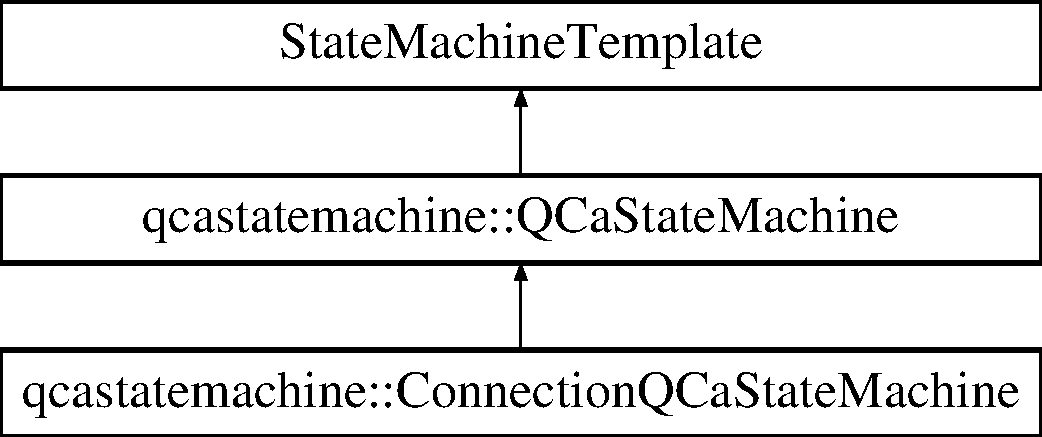
\includegraphics[height=3.000000cm]{classqcastatemachine_1_1ConnectionQCaStateMachine}
\end{center}
\end{figure}
\subsection*{Public Member Functions}
\begin{DoxyCompactItemize}
\item 
\hypertarget{classqcastatemachine_1_1ConnectionQCaStateMachine_a27c364551172947037fe5ccedc16d60a}{
{\bfseries ConnectionQCaStateMachine} (void $\ast$parent)}
\label{classqcastatemachine_1_1ConnectionQCaStateMachine_a27c364551172947037fe5ccedc16d60a}

\item 
\hypertarget{classqcastatemachine_1_1ConnectionQCaStateMachine_a551b85c4d4a43d58c45fe53764690a70}{
bool {\bfseries process} (int requestedState)}
\label{classqcastatemachine_1_1ConnectionQCaStateMachine_a551b85c4d4a43d58c45fe53764690a70}

\end{DoxyCompactItemize}


The documentation for this class was generated from the following files:\begin{DoxyCompactItemize}
\item 
/tmp/epicsqt/trunk/framework/data/include/QCaStateMachine.h\item 
/tmp/epicsqt/trunk/framework/data/src/QCaStateMachine.cpp\end{DoxyCompactItemize}

\hypertarget{classContainerProfile}{
\section{ContainerProfile Class Reference}
\label{classContainerProfile}\index{ContainerProfile@{ContainerProfile}}
}
Inheritance diagram for ContainerProfile:\begin{figure}[H]
\begin{center}
\leavevmode
\includegraphics[height=12.000000cm]{classContainerProfile}
\end{center}
\end{figure}
\subsection*{Public Member Functions}
\begin{DoxyCompactItemize}
\item 
\hypertarget{classContainerProfile_aa5b6583e82e83be981529929506a7a97}{
void {\bfseries takeLocalCopy} ()}
\label{classContainerProfile_aa5b6583e82e83be981529929506a7a97}

\item 
\hypertarget{classContainerProfile_a5f0e629653b907020b637cb3b2e46770}{
void {\bfseries setupProfile} (QObject $\ast$guiLaunchConsumerIn, QStringList pathListIn, QString parentPathIn, QString macroSubstitutionsIn)}
\label{classContainerProfile_a5f0e629653b907020b637cb3b2e46770}

\item 
\hypertarget{classContainerProfile_ab17f938668c578caad9af908a41fd409}{
void {\bfseries setupLocalProfile} (QObject $\ast$guiLaunchConsumerIn, QStringList pathListIn, QString parentPathIn, QString macroSubstitutionsIn)}
\label{classContainerProfile_ab17f938668c578caad9af908a41fd409}

\item 
\hypertarget{classContainerProfile_ab9d4f54da86371dab879cdbf543750c6}{
void {\bfseries updateConsumers} (QObject $\ast$guiLaunchConsumerIn)}
\label{classContainerProfile_ab9d4f54da86371dab879cdbf543750c6}

\item 
\hypertarget{classContainerProfile_a75f5e5d582db66fcee3423638ac45436}{
QObject $\ast$ {\bfseries replaceGuiLaunchConsumer} (QObject $\ast$newGuiLaunchConsumerIn)}
\label{classContainerProfile_a75f5e5d582db66fcee3423638ac45436}

\item 
\hypertarget{classContainerProfile_ae1f30e900c0ecfa79a5a1cfecc5f0d0a}{
void {\bfseries addMacroSubstitutions} (QString macroSubstitutionsIn)}
\label{classContainerProfile_ae1f30e900c0ecfa79a5a1cfecc5f0d0a}

\item 
\hypertarget{classContainerProfile_a477273957a10b9ed4c2a9bac19ba5a6a}{
void {\bfseries removeMacroSubstitutions} ()}
\label{classContainerProfile_a477273957a10b9ed4c2a9bac19ba5a6a}

\item 
\hypertarget{classContainerProfile_a884879dcca1814af0eb0cbe319dd95f2}{
void {\bfseries addPriorityMacroSubstitutions} (QString macroSubstitutionsIn)}
\label{classContainerProfile_a884879dcca1814af0eb0cbe319dd95f2}

\item 
\hypertarget{classContainerProfile_a6352d509a91428daf6bb8b57d440c4c3}{
void {\bfseries removePriorityMacroSubstitutions} ()}
\label{classContainerProfile_a6352d509a91428daf6bb8b57d440c4c3}

\item 
\hypertarget{classContainerProfile_a989941cd1a5c85125e144069f98fbc09}{
QObject $\ast$ {\bfseries getGuiLaunchConsumer} ()}
\label{classContainerProfile_a989941cd1a5c85125e144069f98fbc09}

\item 
\hypertarget{classContainerProfile_ae9a61bc7d3f0a13c03e19a54f7ad32c0}{
QString {\bfseries getPath} ()}
\label{classContainerProfile_ae9a61bc7d3f0a13c03e19a54f7ad32c0}

\item 
\hypertarget{classContainerProfile_aa50e72d82702a109e360381958e6fd69}{
QStringList {\bfseries getPathList} ()}
\label{classContainerProfile_aa50e72d82702a109e360381958e6fd69}

\item 
\hypertarget{classContainerProfile_a6b0109ef1cc0750f4855554f22d5724e}{
QString {\bfseries getParentPath} ()}
\label{classContainerProfile_a6b0109ef1cc0750f4855554f22d5724e}

\item 
\hypertarget{classContainerProfile_a39fb2a71796d844fbd46ad4528cf7a64}{
void {\bfseries setPublishedParentPath} (QString publishedParentPathIn)}
\label{classContainerProfile_a39fb2a71796d844fbd46ad4528cf7a64}

\item 
\hypertarget{classContainerProfile_a3d429a09d4a5fa8b8fb732e8e65486c6}{
QString {\bfseries getMacroSubstitutions} ()}
\label{classContainerProfile_a3d429a09d4a5fa8b8fb732e8e65486c6}

\item 
\hypertarget{classContainerProfile_a78ecf171340a947b39346bf9dac0d1aa}{
bool {\bfseries isProfileDefined} ()}
\label{classContainerProfile_a78ecf171340a947b39346bf9dac0d1aa}

\item 
\hypertarget{classContainerProfile_ae03f8cdb662ab187881e617a6a2e0e04}{
bool {\bfseries areUserLevelPasswordsSet} ()}
\label{classContainerProfile_ae03f8cdb662ab187881e617a6a2e0e04}

\item 
\hypertarget{classContainerProfile_ab90051c321470602cd06879cf66dc2db}{
QStringList {\bfseries getEnvPathList} ()}
\label{classContainerProfile_ab90051c321470602cd06879cf66dc2db}

\item 
\hypertarget{classContainerProfile_a1da65df910a3604eb679f3bba7126df7}{
QString {\bfseries getUserLevelPassword} (\hyperlink{classuserLevelTypes_a033cf2a40f620286b1839dd360c8497b}{userLevelTypes::userLevels} level)}
\label{classContainerProfile_a1da65df910a3604eb679f3bba7126df7}

\item 
\hypertarget{classContainerProfile_a689e5c017c0655d76288042b9088a829}{
void {\bfseries setUserLevelPassword} (\hyperlink{classuserLevelTypes_a033cf2a40f620286b1839dd360c8497b}{userLevelTypes::userLevels} level, QString passwordIn)}
\label{classContainerProfile_a689e5c017c0655d76288042b9088a829}

\item 
\hypertarget{classContainerProfile_a64f106811c4f116a50d11b349eafe9d0}{
void {\bfseries addContainedWidget} (\hyperlink{classQEWidget}{QEWidget} $\ast$containedWidget)}
\label{classContainerProfile_a64f106811c4f116a50d11b349eafe9d0}

\item 
\hypertarget{classContainerProfile_ab1d9ce7ef55e256772a570d02b4552dd}{
\hyperlink{classQEWidget}{QEWidget} $\ast$ {\bfseries getNextContainedWidget} ()}
\label{classContainerProfile_ab1d9ce7ef55e256772a570d02b4552dd}

\item 
\hypertarget{classContainerProfile_ac70241a11d904cb7b71ad213b6104923}{
void {\bfseries removeContainedWidget} (\hyperlink{classQEWidget}{QEWidget} $\ast$containedWidget)}
\label{classContainerProfile_ac70241a11d904cb7b71ad213b6104923}

\item 
\hypertarget{classContainerProfile_a5983f949b8a23713bdb78434b1b9f12e}{
unsigned int {\bfseries getMessageFormId} ()}
\label{classContainerProfile_a5983f949b8a23713bdb78434b1b9f12e}

\item 
\hypertarget{classContainerProfile_a0a40488cac9ddc78d8e3d39cde8759d6}{
unsigned int {\bfseries getPublishedMessageFormId} ()}
\label{classContainerProfile_a0a40488cac9ddc78d8e3d39cde8759d6}

\item 
\hypertarget{classContainerProfile_a8069d53b56a9805e969e1aead88baf33}{
void {\bfseries setPublishedMessageFormId} (unsigned int publishedMessageFormIdIn)}
\label{classContainerProfile_a8069d53b56a9805e969e1aead88baf33}

\item 
\hypertarget{classContainerProfile_a8e1a31812e9b1a38557da7bd54f9b765}{
bool {\bfseries setDontActivateYet} (bool dontActivateIn)}
\label{classContainerProfile_a8e1a31812e9b1a38557da7bd54f9b765}

\item 
\hypertarget{classContainerProfile_a5a22ff4bcda3678dc369982145c3988f}{
bool {\bfseries getDontActivateYet} ()}
\label{classContainerProfile_a5a22ff4bcda3678dc369982145c3988f}

\item 
\hypertarget{classContainerProfile_af7f96acecf83683e3a840221bfce0a71}{
void {\bfseries releaseProfile} ()}
\label{classContainerProfile_af7f96acecf83683e3a840221bfce0a71}

\item 
\hypertarget{classContainerProfile_a5aa04fe4fe8dcfc1d64fdf8345d54c06}{
void {\bfseries publishOwnProfile} ()}
\label{classContainerProfile_a5aa04fe4fe8dcfc1d64fdf8345d54c06}

\item 
\hypertarget{classContainerProfile_a1c5c3cf59b4e1d82ed7a87b473aa173d}{
void {\bfseries setUserLevel} (\hyperlink{classuserLevelTypes_a033cf2a40f620286b1839dd360c8497b}{userLevelTypes::userLevels} level)}
\label{classContainerProfile_a1c5c3cf59b4e1d82ed7a87b473aa173d}

\item 
\hypertarget{classContainerProfile_a97b20c056e2b243fcdebb4201eea9fee}{
\hyperlink{classuserLevelTypes_a033cf2a40f620286b1839dd360c8497b}{userLevelTypes::userLevels} {\bfseries getUserLevel} ()}
\label{classContainerProfile_a97b20c056e2b243fcdebb4201eea9fee}

\item 
\hypertarget{classContainerProfile_a9ec303b7781d01b9c1ee20fa149ce48d}{
virtual void {\bfseries userLevelChanged} (\hyperlink{classuserLevelTypes_a033cf2a40f620286b1839dd360c8497b}{userLevelTypes::userLevels})}
\label{classContainerProfile_a9ec303b7781d01b9c1ee20fa149ce48d}

\item 
\hypertarget{classContainerProfile_a7699b1fa0bf2b680562a1bf05f5e4c9a}{
\hyperlink{classPersistanceManager}{PersistanceManager} $\ast$ {\bfseries getPersistanceManager} ()}
\label{classContainerProfile_a7699b1fa0bf2b680562a1bf05f5e4c9a}

\end{DoxyCompactItemize}


The documentation for this class was generated from the following files:\begin{DoxyCompactItemize}
\item 
/tmp/epicsqt/trunk/framework/widgets/include/ContainerProfile.h\item 
/tmp/epicsqt/trunk/framework/widgets/src/ContainerProfile.cpp\end{DoxyCompactItemize}

\hypertarget{classcontextMenu}{
\section{contextMenu Class Reference}
\label{classcontextMenu}\index{contextMenu@{contextMenu}}
}
Inheritance diagram for contextMenu:\begin{figure}[H]
\begin{center}
\leavevmode
\includegraphics[height=12.000000cm]{classcontextMenu}
\end{center}
\end{figure}
\subsection*{Public Types}
\begin{DoxyCompactItemize}
\item 
enum {\bfseries contextMenuOptions} \{ \par
{\bfseries CM\_\-NONE}, 
{\bfseries CM\_\-COPY\_\-VARIABLE}, 
{\bfseries CM\_\-COPY\_\-DATA}, 
{\bfseries CM\_\-PASTE}, 
\par
{\bfseries CM\_\-DRAG\_\-VARIABLE}, 
{\bfseries CM\_\-DRAG\_\-DATA}, 
{\bfseries CM\_\-SPECIFIC\_\-WIDGETS\_\-START\_\-HERE}
 \}
\end{DoxyCompactItemize}
\subsection*{Public Member Functions}
\begin{DoxyCompactItemize}
\item 
\hypertarget{classcontextMenu_aa999ab4c184150fe9cd7ae196ba4a4b2}{
void {\bfseries addContextMenuToWidget} (QWidget $\ast$w)}
\label{classcontextMenu_aa999ab4c184150fe9cd7ae196ba4a4b2}

\item 
\hypertarget{classcontextMenu_a4d897e1a47d145a524c0d4c1e377c159}{
bool {\bfseries isDraggingVariable} ()}
\label{classcontextMenu_a4d897e1a47d145a524c0d4c1e377c159}

\item 
\hypertarget{classcontextMenu_adafa3f64e846f80d832f0529c6f2e0ec}{
QMenu $\ast$ {\bfseries getContextMenu} ()}
\label{classcontextMenu_adafa3f64e846f80d832f0529c6f2e0ec}

\item 
\hypertarget{classcontextMenu_a4d115deb65fdb2034f4b42f075cb7c51}{
virtual QString {\bfseries copyVariable} ()}
\label{classcontextMenu_a4d115deb65fdb2034f4b42f075cb7c51}

\item 
\hypertarget{classcontextMenu_a69b0308f474ce677da4257581e928e41}{
virtual QVariant {\bfseries copyData} ()}
\label{classcontextMenu_a69b0308f474ce677da4257581e928e41}

\item 
\hypertarget{classcontextMenu_a2e3107c7d83692cff31cdcd669be14b3}{
virtual void {\bfseries paste} (QVariant)}
\label{classcontextMenu_a2e3107c7d83692cff31cdcd669be14b3}

\end{DoxyCompactItemize}
\subsection*{Friends}
\begin{DoxyCompactItemize}
\item 
\hypertarget{classcontextMenu_a034bc826cc430068d488b68c8ca8c4e4}{
class \hyperlink{classcontextMenu_a034bc826cc430068d488b68c8ca8c4e4}{contextMenuObject}}
\label{classcontextMenu_a034bc826cc430068d488b68c8ca8c4e4}

\end{DoxyCompactItemize}


The documentation for this class was generated from the following files:\begin{DoxyCompactItemize}
\item 
/tmp/epicsqt/trunk/framework/widgets/include/contextMenu.h\item 
/tmp/epicsqt/trunk/framework/widgets/src/contextMenu.cpp\end{DoxyCompactItemize}

\hypertarget{classcontextMenuObject}{
\section{contextMenuObject Class Reference}
\label{classcontextMenuObject}\index{contextMenuObject@{contextMenuObject}}
}
\subsection*{Public Slots}
\begin{DoxyCompactItemize}
\item 
\hypertarget{classcontextMenuObject_a832f6bf39f7f9140248cf0cc5fc6956b}{
void {\bfseries contextMenuTriggered} (QAction $\ast$selectedItem)}
\label{classcontextMenuObject_a832f6bf39f7f9140248cf0cc5fc6956b}

\item 
\hypertarget{classcontextMenuObject_a504e51923167cd0ea74d955a4e8d757f}{
void {\bfseries showContextMenu} (const QPoint \&pos)}
\label{classcontextMenuObject_a504e51923167cd0ea74d955a4e8d757f}

\item 
\hypertarget{classcontextMenuObject_a96ffb6c5d39dece7b13a8943ebe0a85b}{
void {\bfseries setChecked} ()}
\label{classcontextMenuObject_a96ffb6c5d39dece7b13a8943ebe0a85b}

\end{DoxyCompactItemize}
\subsection*{Public Member Functions}
\begin{DoxyCompactItemize}
\item 
\hypertarget{classcontextMenuObject_a36c725c35959ad19abf9b13642539334}{
void {\bfseries addContextMenuToWidget} (QWidget $\ast$w)}
\label{classcontextMenuObject_a36c725c35959ad19abf9b13642539334}

\item 
\hypertarget{classcontextMenuObject_a7840a08ca5c558742a2850c2ace91096}{
void {\bfseries manageChecked} (bool draggingVariable)}
\label{classcontextMenuObject_a7840a08ca5c558742a2850c2ace91096}

\item 
\hypertarget{classcontextMenuObject_a54a542f6c725ee95ec0ed3bb9697f208}{
void {\bfseries setMenu} (\hyperlink{classcontextMenu}{contextMenu} $\ast$menuIn)}
\label{classcontextMenuObject_a54a542f6c725ee95ec0ed3bb9697f208}

\item 
\hypertarget{classcontextMenuObject_ad5968dd68e748e20d410dbb73d84a48f}{
bool {\bfseries isDraggingVariable} ()}
\label{classcontextMenuObject_ad5968dd68e748e20d410dbb73d84a48f}

\end{DoxyCompactItemize}


The documentation for this class was generated from the following files:\begin{DoxyCompactItemize}
\item 
/tmp/epicsqt/trunk/framework/widgets/include/contextMenu.h\item 
/tmp/epicsqt/trunk/framework/widgets/src/contextMenu.cpp\end{DoxyCompactItemize}

\hypertarget{structQEPeriodic_1_1elementInfoStruct}{
\section{QEPeriodic::elementInfoStruct Struct Reference}
\label{structQEPeriodic_1_1elementInfoStruct}\index{QEPeriodic::elementInfoStruct@{QEPeriodic::elementInfoStruct}}
}
\subsection*{Public Attributes}
\begin{DoxyCompactItemize}
\item 
\hypertarget{structQEPeriodic_1_1elementInfoStruct_a2ed6f5ccfa01f9c05336709d0fe7d22b}{
unsigned int {\bfseries number}}
\label{structQEPeriodic_1_1elementInfoStruct_a2ed6f5ccfa01f9c05336709d0fe7d22b}

\item 
\hypertarget{structQEPeriodic_1_1elementInfoStruct_adac6b95485680936540fde9b1ce357cd}{
double {\bfseries atomicWeight}}
\label{structQEPeriodic_1_1elementInfoStruct_adac6b95485680936540fde9b1ce357cd}

\item 
\hypertarget{structQEPeriodic_1_1elementInfoStruct_a53d312c3b9e5a47ba5c8657f16e5c0e6}{
QString {\bfseries name}}
\label{structQEPeriodic_1_1elementInfoStruct_a53d312c3b9e5a47ba5c8657f16e5c0e6}

\item 
\hypertarget{structQEPeriodic_1_1elementInfoStruct_afbc2ae5bc1e94552f4ce9fa209ba052d}{
QString {\bfseries symbol}}
\label{structQEPeriodic_1_1elementInfoStruct_afbc2ae5bc1e94552f4ce9fa209ba052d}

\item 
\hypertarget{structQEPeriodic_1_1elementInfoStruct_a264cba29d4c938d5e95896d34d220eea}{
double {\bfseries meltingPoint}}
\label{structQEPeriodic_1_1elementInfoStruct_a264cba29d4c938d5e95896d34d220eea}

\item 
\hypertarget{structQEPeriodic_1_1elementInfoStruct_aa12a2085c11e772e4ef4b3d2809ab56f}{
double {\bfseries boilingPoint}}
\label{structQEPeriodic_1_1elementInfoStruct_aa12a2085c11e772e4ef4b3d2809ab56f}

\item 
\hypertarget{structQEPeriodic_1_1elementInfoStruct_ae353fbd57ff732b6f21d50b6cf83c33c}{
double {\bfseries density}}
\label{structQEPeriodic_1_1elementInfoStruct_ae353fbd57ff732b6f21d50b6cf83c33c}

\item 
\hypertarget{structQEPeriodic_1_1elementInfoStruct_aceb9865dda759f31309e6202375f0fc1}{
unsigned int {\bfseries group}}
\label{structQEPeriodic_1_1elementInfoStruct_aceb9865dda759f31309e6202375f0fc1}

\item 
\hypertarget{structQEPeriodic_1_1elementInfoStruct_a8259579d351ab4ba6b9f04820e18e9b8}{
double {\bfseries ionizationEnergy}}
\label{structQEPeriodic_1_1elementInfoStruct_a8259579d351ab4ba6b9f04820e18e9b8}

\item 
\hypertarget{structQEPeriodic_1_1elementInfoStruct_ad173c2d6d07aed9c726cca04a9851ffa}{
unsigned int {\bfseries tableRow}}
\label{structQEPeriodic_1_1elementInfoStruct_ad173c2d6d07aed9c726cca04a9851ffa}

\item 
\hypertarget{structQEPeriodic_1_1elementInfoStruct_abcfeb91b2e76b72b33dd737f232fb3bb}{
unsigned int {\bfseries tableCol}}
\label{structQEPeriodic_1_1elementInfoStruct_abcfeb91b2e76b72b33dd737f232fb3bb}

\end{DoxyCompactItemize}


The documentation for this struct was generated from the following file:\begin{DoxyCompactItemize}
\item 
/tmp/epicsqt/trunk/framework/widgets/QEPeriodic/QEPeriodic.h\end{DoxyCompactItemize}

\hypertarget{classflipRotateMenu}{
\section{flipRotateMenu Class Reference}
\label{classflipRotateMenu}\index{flipRotateMenu@{flipRotateMenu}}
}
\subsection*{Public Member Functions}
\begin{DoxyCompactItemize}
\item 
\hypertarget{classflipRotateMenu_ae081b477fc71324f7dc8593be4ae320d}{
{\bfseries flipRotateMenu} (QWidget $\ast$parent=0)}
\label{classflipRotateMenu_ae081b477fc71324f7dc8593be4ae320d}

\item 
\hypertarget{classflipRotateMenu_ab7159ea467dde7027a9812799461dcc3}{
imageContextMenu::imageContextMenuOptions {\bfseries getFlipRotate} (const QPoint \&pos)}
\label{classflipRotateMenu_ab7159ea467dde7027a9812799461dcc3}

\item 
\hypertarget{classflipRotateMenu_a028c6c9433580caad8b936e2472b5561}{
void {\bfseries setChecked} (const int rotation, const bool flipH, const bool flipV)}
\label{classflipRotateMenu_a028c6c9433580caad8b936e2472b5561}

\end{DoxyCompactItemize}


The documentation for this class was generated from the following files:\begin{DoxyCompactItemize}
\item 
/tmp/epicsqt/trunk/framework/widgets/QEImage/flipRotateMenu.h\item 
/tmp/epicsqt/trunk/framework/widgets/QEImage/flipRotateMenu.cpp\end{DoxyCompactItemize}

\hypertarget{classimageContextMenu}{
\section{imageContextMenu Class Reference}
\label{classimageContextMenu}\index{imageContextMenu@{imageContextMenu}}
}
\subsection*{Public Types}
\begin{DoxyCompactItemize}
\item 
enum {\bfseries imageContextMenuOptions} \{ \par
{\bfseries ICM\_\-NONE} =  contextMenu::CM\_\-SPECIFIC\_\-WIDGETS\_\-START\_\-HERE, 
{\bfseries ICM\_\-SAVE}, 
{\bfseries ICM\_\-PAUSE}, 
{\bfseries ICM\_\-ENABLE\_\-TIME}, 
\par
{\bfseries ICM\_\-ENABLE\_\-CURSOR\_\-PIXEL}, 
{\bfseries ICM\_\-ENABLE\_\-CONTRAST\_\-REVERSAL}, 
{\bfseries ICM\_\-ENABLE\_\-VERT}, 
{\bfseries ICM\_\-ENABLE\_\-HOZ}, 
\par
{\bfseries ICM\_\-ENABLE\_\-AREA}, 
{\bfseries ICM\_\-ENABLE\_\-LINE}, 
{\bfseries ICM\_\-ENABLE\_\-TARGET}, 
{\bfseries ICM\_\-DISPLAY\_\-BUTTON\_\-BAR}, 
\par
{\bfseries ICM\_\-DISPLAY\_\-BRIGHTNESS\_\-CONTRAST}, 
{\bfseries ICM\_\-ZOOM\_\-SELECTED}, 
{\bfseries ICM\_\-ZOOM\_\-FIT}, 
{\bfseries ICM\_\-ZOOM\_\-10}, 
\par
{\bfseries ICM\_\-ZOOM\_\-25}, 
{\bfseries ICM\_\-ZOOM\_\-50}, 
{\bfseries ICM\_\-ZOOM\_\-75}, 
{\bfseries ICM\_\-ZOOM\_\-100}, 
\par
{\bfseries ICM\_\-ZOOM\_\-150}, 
{\bfseries ICM\_\-ZOOM\_\-200}, 
{\bfseries ICM\_\-ZOOM\_\-300}, 
{\bfseries ICM\_\-ZOOM\_\-400}, 
\par
{\bfseries ICM\_\-ROTATE\_\-NONE}, 
{\bfseries ICM\_\-ROTATE\_\-RIGHT}, 
{\bfseries ICM\_\-ROTATE\_\-LEFT}, 
{\bfseries ICM\_\-ROTATE\_\-180}, 
\par
{\bfseries ICM\_\-FLIP\_\-HORIZONTAL}, 
{\bfseries ICM\_\-FLIP\_\-VERTICAL}, 
{\bfseries ICM\_\-SELECT\_\-PAN}, 
{\bfseries ICM\_\-SELECT\_\-HSLICE}, 
\par
{\bfseries ICM\_\-SELECT\_\-VSLICE}, 
{\bfseries ICM\_\-SELECT\_\-AREA1}, 
{\bfseries ICM\_\-SELECT\_\-AREA2}, 
{\bfseries ICM\_\-SELECT\_\-AREA3}, 
\par
{\bfseries ICM\_\-SELECT\_\-AREA4}, 
{\bfseries ICM\_\-SELECT\_\-PROFILE}, 
{\bfseries ICM\_\-SELECT\_\-TARGET}, 
{\bfseries ICM\_\-SELECT\_\-BEAM}, 
\par
{\bfseries ICM\_\-CLEAR\_\-MARKUP}, 
{\bfseries ICM\_\-THICKNESS\_\-ONE\_\-MARKUP}, 
{\bfseries ICM\_\-THICKNESS\_\-SELECT\_\-MARKUP}, 
{\bfseries ICM\_\-COPY\_\-PLOT\_\-DATA}
 \}
\end{DoxyCompactItemize}
\subsection*{Public Member Functions}
\begin{DoxyCompactItemize}
\item 
\hypertarget{classimageContextMenu_a74a2d31c09f2d410ea3d1e5b6f631530}{
{\bfseries imageContextMenu} (QWidget $\ast$parent=0)}
\label{classimageContextMenu_a74a2d31c09f2d410ea3d1e5b6f631530}

\item 
\hypertarget{classimageContextMenu_a5f57af407bdd1d3bc5e8b9b22ac573ab}{
void {\bfseries getContextMenuOption} (const QPoint \&, imageContextMenuOptions $\ast$option, bool $\ast$checked)}
\label{classimageContextMenu_a5f57af407bdd1d3bc5e8b9b22ac573ab}

\item 
\hypertarget{classimageContextMenu_a92f602856915fa4717ca23f1ee56e5a5}{
void {\bfseries addMenuItem} (const QString \&title, const bool checkable, const bool checked, const imageContextMenuOptions option)}
\label{classimageContextMenu_a92f602856915fa4717ca23f1ee56e5a5}

\item 
\hypertarget{classimageContextMenu_af34ef9194140b925c833b78d93d27db0}{
void {\bfseries addOptionMenuItem} (const QString \&title, const bool checkable, const bool checked, const imageContextMenuOptions option)}
\label{classimageContextMenu_af34ef9194140b925c833b78d93d27db0}

\end{DoxyCompactItemize}


The documentation for this class was generated from the following files:\begin{DoxyCompactItemize}
\item 
/tmp/epicsqt/trunk/framework/widgets/QEImage/imageContextMenu.h\item 
/tmp/epicsqt/trunk/framework/widgets/QEImage/imageContextMenu.cpp\end{DoxyCompactItemize}

\hypertarget{classimageInfo}{
\section{imageInfo Class Reference}
\label{classimageInfo}\index{imageInfo@{imageInfo}}
}
Inheritance diagram for imageInfo:\begin{figure}[H]
\begin{center}
\leavevmode
\includegraphics[height=2.000000cm]{classimageInfo}
\end{center}
\end{figure}
\subsection*{Public Member Functions}
\begin{DoxyCompactItemize}
\item 
\hypertarget{classimageInfo_ab9c63ac1d0a4a14844c4135d5c44202e}{
void {\bfseries showInfo} (bool show)}
\label{classimageInfo_ab9c63ac1d0a4a14844c4135d5c44202e}

\item 
\hypertarget{classimageInfo_a6ed71ac5cb9612324f6e9c9755747470}{
QLayout $\ast$ {\bfseries getInfoWidget} ()}
\label{classimageInfo_a6ed71ac5cb9612324f6e9c9755747470}

\item 
\hypertarget{classimageInfo_ac031e6c46d567d2a0215bc025eadb982}{
void {\bfseries infoShow} (const bool show)}
\label{classimageInfo_ac031e6c46d567d2a0215bc025eadb982}

\item 
\hypertarget{classimageInfo_abeae02809096ab62ba004af2b70197da}{
void {\bfseries infoUpdateTarget} ()}
\label{classimageInfo_abeae02809096ab62ba004af2b70197da}

\item 
\hypertarget{classimageInfo_a1ec49f20e5899a70ad6cbbc2182e1899}{
void {\bfseries infoUpdateTarget} (const int x, const int y)}
\label{classimageInfo_a1ec49f20e5899a70ad6cbbc2182e1899}

\item 
\hypertarget{classimageInfo_a101b262f8a75d9bd7973c08d3e9a0696}{
void {\bfseries infoUpdateBeam} ()}
\label{classimageInfo_a101b262f8a75d9bd7973c08d3e9a0696}

\item 
\hypertarget{classimageInfo_a0fdb14d460ee5f268e3345302f0e20df}{
void {\bfseries infoUpdateBeam} (const int x, const int y)}
\label{classimageInfo_a0fdb14d460ee5f268e3345302f0e20df}

\item 
\hypertarget{classimageInfo_a0c826adb5b824b6d454e0f8c95fe081d}{
void {\bfseries infoUpdateVertProfile} ()}
\label{classimageInfo_a0c826adb5b824b6d454e0f8c95fe081d}

\item 
\hypertarget{classimageInfo_a415347b0bbd417023a4790f955ea1695}{
void {\bfseries infoUpdateVertProfile} (const int x, const unsigned int thickness)}
\label{classimageInfo_a415347b0bbd417023a4790f955ea1695}

\item 
\hypertarget{classimageInfo_a2605cb9a76df62f861f1fd36b1083cec}{
void {\bfseries infoUpdateHozProfile} ()}
\label{classimageInfo_a2605cb9a76df62f861f1fd36b1083cec}

\item 
\hypertarget{classimageInfo_af3bc6c7ab51ade831513593e5ec37bc8}{
void {\bfseries infoUpdateHozProfile} (const int y, const unsigned int thickness)}
\label{classimageInfo_af3bc6c7ab51ade831513593e5ec37bc8}

\item 
\hypertarget{classimageInfo_ae8b92f5270d9f68e36408d5d7b0070bf}{
void {\bfseries infoUpdateProfile} ()}
\label{classimageInfo_ae8b92f5270d9f68e36408d5d7b0070bf}

\item 
\hypertarget{classimageInfo_ae3b4a16888ce04800841e586aafbeb1b}{
void {\bfseries infoUpdateProfile} (const QPoint start, const QPoint end, const unsigned int thickness)}
\label{classimageInfo_ae3b4a16888ce04800841e586aafbeb1b}

\item 
\hypertarget{classimageInfo_a553687717aa2326bc9ae40c45ef738b3}{
void {\bfseries infoUpdateRegion} (const unsigned int region)}
\label{classimageInfo_a553687717aa2326bc9ae40c45ef738b3}

\item 
\hypertarget{classimageInfo_a4dcd105500ad0179741128405478f5cb}{
void {\bfseries infoUpdateRegion} (const unsigned int region, const int x1, const int y1, const int x2, const int y2)}
\label{classimageInfo_a4dcd105500ad0179741128405478f5cb}

\item 
\hypertarget{classimageInfo_a70e991916e7e8d316f2acd82a22913d2}{
void {\bfseries infoUpdatePixel} ()}
\label{classimageInfo_a70e991916e7e8d316f2acd82a22913d2}

\item 
\hypertarget{classimageInfo_a0bf41ad48a5a379839425f1d91ebe737}{
void {\bfseries infoUpdatePixel} (const QPoint pos, int value)}
\label{classimageInfo_a0bf41ad48a5a379839425f1d91ebe737}

\end{DoxyCompactItemize}


The documentation for this class was generated from the following files:\begin{DoxyCompactItemize}
\item 
/tmp/epicsqt/trunk/framework/widgets/QEImage/imageInfo.h\item 
/tmp/epicsqt/trunk/framework/widgets/QEImage/imageInfo.cpp\end{DoxyCompactItemize}

\hypertarget{classimageMarkup}{
\section{imageMarkup Class Reference}
\label{classimageMarkup}\index{imageMarkup@{imageMarkup}}
}
Inheritance diagram for imageMarkup:\begin{figure}[H]
\begin{center}
\leavevmode
\includegraphics[height=2.000000cm]{classimageMarkup}
\end{center}
\end{figure}
\subsection*{Public Types}
\begin{DoxyCompactItemize}
\item 
enum {\bfseries markupIds} \{ \par
{\bfseries MARKUP\_\-ID\_\-REGION1}, 
{\bfseries MARKUP\_\-ID\_\-REGION2}, 
{\bfseries MARKUP\_\-ID\_\-REGION3}, 
{\bfseries MARKUP\_\-ID\_\-REGION4}, 
\par
{\bfseries MARKUP\_\-ID\_\-H\_\-SLICE}, 
{\bfseries MARKUP\_\-ID\_\-V\_\-SLICE}, 
{\bfseries MARKUP\_\-ID\_\-LINE}, 
{\bfseries MARKUP\_\-ID\_\-TARGET}, 
\par
{\bfseries MARKUP\_\-ID\_\-BEAM}, 
{\bfseries MARKUP\_\-ID\_\-TIMESTAMP}, 
{\bfseries MARKUP\_\-ID\_\-COUNT}, 
{\bfseries MARKUP\_\-ID\_\-NONE}
 \}
\end{DoxyCompactItemize}
\subsection*{Public Member Functions}
\begin{DoxyCompactItemize}
\item 
\hypertarget{classimageMarkup_ad00e95e6b26753cec7d6390c750bb922}{
void {\bfseries setShowTime} (bool visibleIn)}
\label{classimageMarkup_ad00e95e6b26753cec7d6390c750bb922}

\item 
\hypertarget{classimageMarkup_aca883d394519475a8988eb3e7c359928}{
bool {\bfseries getShowTime} ()}
\label{classimageMarkup_aca883d394519475a8988eb3e7c359928}

\item 
\hypertarget{classimageMarkup_a288b684b824ff0ad926a949bdc4451fe}{
markupIds {\bfseries getMode} ()}
\label{classimageMarkup_a288b684b824ff0ad926a949bdc4451fe}

\item 
\hypertarget{classimageMarkup_a13a6605444abe8efc548bd55de0f4e9b}{
void {\bfseries setMode} (markupIds modeIn)}
\label{classimageMarkup_a13a6605444abe8efc548bd55de0f4e9b}

\item 
\hypertarget{classimageMarkup_a0b964a9a07732f938ec14bb02238bbbe}{
void {\bfseries setMarkupColor} (markupIds mode, QColor markupColorIn)}
\label{classimageMarkup_a0b964a9a07732f938ec14bb02238bbbe}

\item 
\hypertarget{classimageMarkup_a45b15582a0a92c4d54dea0f2f08cd17a}{
QColor {\bfseries getMarkupColor} (markupIds mode)}
\label{classimageMarkup_a45b15582a0a92c4d54dea0f2f08cd17a}

\item 
\hypertarget{classimageMarkup_a8cbfca43178690e43ba082d85ae3ca81}{
bool {\bfseries showMarkupMenu} (const QPoint \&pos, const QPoint \&globalPos)}
\label{classimageMarkup_a8cbfca43178690e43ba082d85ae3ca81}

\item 
\hypertarget{classimageMarkup_a40c518b9858028badf181ba0a59532d2}{
void {\bfseries markupRegionValueChange} (int areaIndex, QRect area)}
\label{classimageMarkup_a40c518b9858028badf181ba0a59532d2}

\item 
\hypertarget{classimageMarkup_a95f190be9a7a80c9a0f133a0513f23e4}{
QCursor {\bfseries getCircleCursor} ()}
\label{classimageMarkup_a95f190be9a7a80c9a0f133a0513f23e4}

\item 
\hypertarget{classimageMarkup_af58bcc05af6b1833034e1a5de0de420f}{
QCursor {\bfseries getTargetCursor} ()}
\label{classimageMarkup_af58bcc05af6b1833034e1a5de0de420f}

\item 
\hypertarget{classimageMarkup_a9f24e2d4fa21e06a0b0992738d0fa0d3}{
QCursor {\bfseries getVLineCursor} ()}
\label{classimageMarkup_a9f24e2d4fa21e06a0b0992738d0fa0d3}

\item 
\hypertarget{classimageMarkup_abef73b9a243d9c1af8d1a218d3cdbd7a}{
QCursor {\bfseries getHLineCursor} ()}
\label{classimageMarkup_abef73b9a243d9c1af8d1a218d3cdbd7a}

\item 
\hypertarget{classimageMarkup_a9ee9d8beac075524f79fd3814067e1da}{
QCursor {\bfseries getLineCursor} ()}
\label{classimageMarkup_a9ee9d8beac075524f79fd3814067e1da}

\item 
\hypertarget{classimageMarkup_a3c8cb649388cc91c10abd6f085ced249}{
QCursor {\bfseries getRegionCursor} ()}
\label{classimageMarkup_a3c8cb649388cc91c10abd6f085ced249}

\item 
\hypertarget{classimageMarkup_aa3e259930011166fcf12df66b86aa6c9}{
virtual void {\bfseries markupSetCursor} (QCursor cursor)=0}
\label{classimageMarkup_aa3e259930011166fcf12df66b86aa6c9}

\end{DoxyCompactItemize}
\subsection*{Public Attributes}
\begin{DoxyCompactItemize}
\item 
\hypertarget{classimageMarkup_a435ac89504244ad48dcab3680f549fe1}{
QImage $\ast$ {\bfseries markupImage}}
\label{classimageMarkup_a435ac89504244ad48dcab3680f549fe1}

\item 
\hypertarget{classimageMarkup_aa68007687a3e28ec62e5ff6abaca412f}{
QVector$<$ \hyperlink{classmarkupItem}{markupItem} $\ast$ $>$ {\bfseries items}}
\label{classimageMarkup_aa68007687a3e28ec62e5ff6abaca412f}

\item 
\hypertarget{classimageMarkup_a06752e238e76e01cde51452eff6fc180}{
QPoint {\bfseries grabOffset}}
\label{classimageMarkup_a06752e238e76e01cde51452eff6fc180}

\item 
\hypertarget{classimageMarkup_a3d7427247a4f9bcb34995e2ed737a67f}{
bool {\bfseries markupAreasStale}}
\label{classimageMarkup_a3d7427247a4f9bcb34995e2ed737a67f}

\item 
\hypertarget{classimageMarkup_a537c83f415a315bff010cdd79a791989}{
QFont {\bfseries legendFont}}
\label{classimageMarkup_a537c83f415a315bff010cdd79a791989}

\item 
\hypertarget{classimageMarkup_a53e1fbae784af4ff90ab16631ce57f2d}{
QFontMetrics $\ast$ {\bfseries legendFontMetrics}}
\label{classimageMarkup_a53e1fbae784af4ff90ab16631ce57f2d}

\end{DoxyCompactItemize}
\subsection*{Protected Member Functions}
\begin{DoxyCompactItemize}
\item 
\hypertarget{classimageMarkup_aeae4ffbe6d20b76c25724d47250b374b}{
bool {\bfseries anyVisibleMarkups} ()}
\label{classimageMarkup_aeae4ffbe6d20b76c25724d47250b374b}

\item 
\hypertarget{classimageMarkup_a4e4f63ab4958c63466c1dfe5e86a4dd0}{
QVector$<$ QRect $>$ \& {\bfseries getMarkupAreas} ()}
\label{classimageMarkup_a4e4f63ab4958c63466c1dfe5e86a4dd0}

\item 
\hypertarget{classimageMarkup_a9a21ffbaedcb65a9c8e2ddedf1dcd2f3}{
QCursor {\bfseries getDefaultMarkupCursor} ()}
\label{classimageMarkup_a9a21ffbaedcb65a9c8e2ddedf1dcd2f3}

\item 
\hypertarget{classimageMarkup_afc6de4b750eccb99e8a50aff52c2218e}{
void {\bfseries setMarkupTime} (\hyperlink{classQCaDateTime}{QCaDateTime} \&time)}
\label{classimageMarkup_afc6de4b750eccb99e8a50aff52c2218e}

\item 
\hypertarget{classimageMarkup_a2dce50b10368db7e162aa1724defab88}{
bool {\bfseries markupMousePressEvent} (QMouseEvent $\ast$event, bool panning)}
\label{classimageMarkup_a2dce50b10368db7e162aa1724defab88}

\item 
\hypertarget{classimageMarkup_aafaaaa8cc99e1f79f69638fcb2a78188}{
bool {\bfseries markupMouseReleaseEvent} (QMouseEvent $\ast$event, bool panning)}
\label{classimageMarkup_aafaaaa8cc99e1f79f69638fcb2a78188}

\item 
\hypertarget{classimageMarkup_a0caa63fa8f11118f3afb46741e649c1b}{
bool {\bfseries markupMouseMoveEvent} (QMouseEvent $\ast$event, bool panning)}
\label{classimageMarkup_a0caa63fa8f11118f3afb46741e649c1b}

\item 
\hypertarget{classimageMarkup_a1da1eb66cead902e79742ecad744b5f5}{
void {\bfseries markupResize} (QSize newSize, double scale)}
\label{classimageMarkup_a1da1eb66cead902e79742ecad744b5f5}

\item 
\hypertarget{classimageMarkup_ace2d0f869a42c8742160c0acd4b6af31}{
virtual void {\bfseries markupChange} (QImage \&markups, QVector$<$ QRect $>$ \&changedAreas)=0}
\label{classimageMarkup_ace2d0f869a42c8742160c0acd4b6af31}

\item 
\hypertarget{classimageMarkup_a015205c484b8406f41fcc897e6e53776}{
virtual void {\bfseries markupAction} (markupIds mode, bool complete, bool clearing, QPoint point1, QPoint point2, unsigned int thickness)=0}
\label{classimageMarkup_a015205c484b8406f41fcc897e6e53776}

\end{DoxyCompactItemize}


The documentation for this class was generated from the following files:\begin{DoxyCompactItemize}
\item 
/tmp/epicsqt/trunk/framework/widgets/QEImage/imageMarkup.h\item 
/tmp/epicsqt/trunk/framework/widgets/QEImage/imageMarkup.cpp\end{DoxyCompactItemize}

\hypertarget{classmanagePixmaps}{
\section{managePixmaps Class Reference}
\label{classmanagePixmaps}\index{managePixmaps@{managePixmaps}}
}
Inheritance diagram for managePixmaps:\begin{figure}[H]
\begin{center}
\leavevmode
\includegraphics[height=3.000000cm]{classmanagePixmaps}
\end{center}
\end{figure}
\subsection*{Public Member Functions}
\begin{DoxyCompactItemize}
\item 
\hypertarget{classmanagePixmaps_a49384115f677a14241dc477de0b8ac01}{
void {\bfseries setDataPixmap} (const QPixmap \&Pixmap, const unsigned int index)}
\label{classmanagePixmaps_a49384115f677a14241dc477de0b8ac01}

\item 
\hypertarget{classmanagePixmaps_a481ab0139363c76d1b93014c26201180}{
QPixmap {\bfseries getDataPixmap} (const unsigned int index)}
\label{classmanagePixmaps_a481ab0139363c76d1b93014c26201180}

\item 
\hypertarget{classmanagePixmaps_a870a168314c0d88d5430823dbb3578f7}{
QPixmap {\bfseries getDataPixmap} (const QString value)}
\label{classmanagePixmaps_a870a168314c0d88d5430823dbb3578f7}

\end{DoxyCompactItemize}


The documentation for this class was generated from the following files:\begin{DoxyCompactItemize}
\item 
/tmp/epicsqt/trunk/framework/widgets/include/managePixmaps.h\item 
/tmp/epicsqt/trunk/framework/widgets/src/managePixmaps.cpp\end{DoxyCompactItemize}

\hypertarget{classmarkupBeam}{
\section{markupBeam Class Reference}
\label{classmarkupBeam}\index{markupBeam@{markupBeam}}
}
Inheritance diagram for markupBeam:\begin{figure}[H]
\begin{center}
\leavevmode
\includegraphics[height=2.000000cm]{classmarkupBeam}
\end{center}
\end{figure}
\subsection*{Public Member Functions}
\begin{DoxyCompactItemize}
\item 
\hypertarget{classmarkupBeam_a7c5abd2cb10de09f7e542bd5bb29299a}{
{\bfseries markupBeam} (\hyperlink{classimageMarkup}{imageMarkup} $\ast$ownerIn, const bool interactiveIn, const bool reportOnMoveIn, const QString legendIn)}
\label{classmarkupBeam_a7c5abd2cb10de09f7e542bd5bb29299a}

\item 
\hypertarget{classmarkupBeam_a241b4191faa7b7588ca4a1398dce83c9}{
void {\bfseries startDrawing} (const QPoint pos)}
\label{classmarkupBeam_a241b4191faa7b7588ca4a1398dce83c9}

\item 
\hypertarget{classmarkupBeam_a426527b6dd3e3113e8a54402c658af9c}{
void {\bfseries setArea} ()}
\label{classmarkupBeam_a426527b6dd3e3113e8a54402c658af9c}

\item 
\hypertarget{classmarkupBeam_a1c9f4a8b96899963faafd20b12845197}{
void {\bfseries drawMarkup} (QPainter \&p)}
\label{classmarkupBeam_a1c9f4a8b96899963faafd20b12845197}

\item 
\hypertarget{classmarkupBeam_aeb3470b326dfe0ca0808f5a7390cf34a}{
void {\bfseries moveTo} (const QPoint pos)}
\label{classmarkupBeam_aeb3470b326dfe0ca0808f5a7390cf34a}

\item 
\hypertarget{classmarkupBeam_a0662cddefb83705e6c14b0870d19b647}{
bool {\bfseries isOver} (const QPoint point, QCursor $\ast$cursor)}
\label{classmarkupBeam_a0662cddefb83705e6c14b0870d19b647}

\item 
\hypertarget{classmarkupBeam_a2c3a6045feb0f3093101951e5c938c8b}{
QPoint {\bfseries origin} ()}
\label{classmarkupBeam_a2c3a6045feb0f3093101951e5c938c8b}

\item 
\hypertarget{classmarkupBeam_a80c28e0af84ad0a21d4069bc9acbe5de}{
QCursor {\bfseries cursorForHandle} (const markupItem::markupHandles handle)}
\label{classmarkupBeam_a80c28e0af84ad0a21d4069bc9acbe5de}

\item 
\hypertarget{classmarkupBeam_af4dbb501db97fc2b21c8f49eba26ec7a}{
QPoint {\bfseries getPoint1} ()}
\label{classmarkupBeam_af4dbb501db97fc2b21c8f49eba26ec7a}

\item 
\hypertarget{classmarkupBeam_a0c3580dc369e3c3fa38845e0962ede7d}{
QPoint {\bfseries getPoint2} ()}
\label{classmarkupBeam_a0c3580dc369e3c3fa38845e0962ede7d}

\item 
\hypertarget{classmarkupBeam_adb29c80ace917570145becb4bea2db71}{
unsigned int {\bfseries getThickness} ()}
\label{classmarkupBeam_adb29c80ace917570145becb4bea2db71}

\item 
\hypertarget{classmarkupBeam_ac5c6ac4426fc7ddf03d712d0b23d6561}{
void {\bfseries setThickness} (const unsigned int thicknessIn)}
\label{classmarkupBeam_ac5c6ac4426fc7ddf03d712d0b23d6561}

\item 
\hypertarget{classmarkupBeam_a674790f9bd7d317245567c95bcc446f1}{
QCursor {\bfseries defaultCursor} ()}
\label{classmarkupBeam_a674790f9bd7d317245567c95bcc446f1}

\item 
\hypertarget{classmarkupBeam_a029a5141fc340d89d0f1ae9b53c1b64f}{
void {\bfseries scaleSpecific} (const double xScale, const double yScale, const double zoomScale)}
\label{classmarkupBeam_a029a5141fc340d89d0f1ae9b53c1b64f}

\end{DoxyCompactItemize}


The documentation for this class was generated from the following files:\begin{DoxyCompactItemize}
\item 
/tmp/epicsqt/trunk/framework/widgets/QEImage/imageMarkup.h\item 
/tmp/epicsqt/trunk/framework/widgets/QEImage/imageMarkup.cpp\end{DoxyCompactItemize}

\hypertarget{classmarkupHLine}{
\section{markupHLine Class Reference}
\label{classmarkupHLine}\index{markupHLine@{markupHLine}}
}
Inheritance diagram for markupHLine:\begin{figure}[H]
\begin{center}
\leavevmode
\includegraphics[height=2.000000cm]{classmarkupHLine}
\end{center}
\end{figure}
\subsection*{Public Member Functions}
\begin{DoxyCompactItemize}
\item 
\hypertarget{classmarkupHLine_abc6c17b619b185940f1678b769ab7e1d}{
{\bfseries markupHLine} (\hyperlink{classimageMarkup}{imageMarkup} $\ast$ownerIn, const bool interactiveIn, const bool reportOnMoveIn, const QString legendIn)}
\label{classmarkupHLine_abc6c17b619b185940f1678b769ab7e1d}

\item 
\hypertarget{classmarkupHLine_aafeb04b96ec1c923b3240c29f949d6cb}{
void {\bfseries startDrawing} (const QPoint pos)}
\label{classmarkupHLine_aafeb04b96ec1c923b3240c29f949d6cb}

\item 
\hypertarget{classmarkupHLine_ace494831be4d38937b008cea65adfb05}{
void {\bfseries setArea} ()}
\label{classmarkupHLine_ace494831be4d38937b008cea65adfb05}

\item 
void \hyperlink{classmarkupHLine_a5ed73a79687003d513e037bda5d4e23a}{drawMarkup} (QPainter \&p)
\item 
\hypertarget{classmarkupHLine_acd184832cbdca72e935c0f24dcb9c908}{
void {\bfseries moveTo} (const QPoint pos)}
\label{classmarkupHLine_acd184832cbdca72e935c0f24dcb9c908}

\item 
\hypertarget{classmarkupHLine_a63105859831a3d425d7c1078054903d6}{
bool {\bfseries isOver} (const QPoint point, QCursor $\ast$cursor)}
\label{classmarkupHLine_a63105859831a3d425d7c1078054903d6}

\item 
\hypertarget{classmarkupHLine_adcc990ff459ac11e924a1538af05b3b7}{
QPoint {\bfseries origin} ()}
\label{classmarkupHLine_adcc990ff459ac11e924a1538af05b3b7}

\item 
\hypertarget{classmarkupHLine_a3c4baf641c08d1d0bb47dd9de6120461}{
QCursor {\bfseries cursorForHandle} (const markupItem::markupHandles handle)}
\label{classmarkupHLine_a3c4baf641c08d1d0bb47dd9de6120461}

\item 
\hypertarget{classmarkupHLine_a17647bf1a5fe00cd436cac2d994eea5e}{
QPoint {\bfseries getPoint1} ()}
\label{classmarkupHLine_a17647bf1a5fe00cd436cac2d994eea5e}

\item 
\hypertarget{classmarkupHLine_a762dacc6a99ee751080af0cc1ada7672}{
QPoint {\bfseries getPoint2} ()}
\label{classmarkupHLine_a762dacc6a99ee751080af0cc1ada7672}

\item 
\hypertarget{classmarkupHLine_ae08a41cf6b2435ecd86bc569c6e31fff}{
unsigned int {\bfseries getThickness} ()}
\label{classmarkupHLine_ae08a41cf6b2435ecd86bc569c6e31fff}

\item 
\hypertarget{classmarkupHLine_ad98d4ac5293c132bb91fdadaf3e5eecd}{
void {\bfseries setThickness} (const unsigned int thicknessIn)}
\label{classmarkupHLine_ad98d4ac5293c132bb91fdadaf3e5eecd}

\item 
\hypertarget{classmarkupHLine_a552b073420b364ca4b00fd39225f37ac}{
QCursor {\bfseries defaultCursor} ()}
\label{classmarkupHLine_a552b073420b364ca4b00fd39225f37ac}

\item 
\hypertarget{classmarkupHLine_a94516864e1a9227cc4e512f82fff70ce}{
void {\bfseries scaleSpecific} (const double xScale, const double yScale, const double zoomScale)}
\label{classmarkupHLine_a94516864e1a9227cc4e512f82fff70ce}

\end{DoxyCompactItemize}


\subsection{Member Function Documentation}
\hypertarget{classmarkupHLine_a5ed73a79687003d513e037bda5d4e23a}{
\index{markupHLine@{markupHLine}!drawMarkup@{drawMarkup}}
\index{drawMarkup@{drawMarkup}!markupHLine@{markupHLine}}
\subsubsection[{drawMarkup}]{\setlength{\rightskip}{0pt plus 5cm}void markupHLine::drawMarkup (
\begin{DoxyParamCaption}
\item[{QPainter \&}]{p}
\end{DoxyParamCaption}
)\hspace{0.3cm}{\ttfamily  \mbox{[}virtual\mbox{]}}}}
\label{classmarkupHLine_a5ed73a79687003d513e037bda5d4e23a}


!! draw the handle in the middle of the existing view, not the entire image 



Implements \hyperlink{classmarkupItem}{markupItem}.



The documentation for this class was generated from the following files:\begin{DoxyCompactItemize}
\item 
/tmp/epicsqt/trunk/framework/widgets/QEImage/imageMarkup.h\item 
/tmp/epicsqt/trunk/framework/widgets/QEImage/imageMarkup.cpp\end{DoxyCompactItemize}

\hypertarget{classmarkupItem}{
\section{markupItem Class Reference}
\label{classmarkupItem}\index{markupItem@{markupItem}}
}
Inheritance diagram for markupItem:\begin{figure}[H]
\begin{center}
\leavevmode
\includegraphics[height=1.600000cm]{classmarkupItem}
\end{center}
\end{figure}
\subsection*{Public Types}
\begin{DoxyCompactItemize}
\item 
enum {\bfseries markupHandles} \{ \par
{\bfseries MARKUP\_\-HANDLE\_\-NONE}, 
{\bfseries MARKUP\_\-HANDLE\_\-START}, 
{\bfseries MARKUP\_\-HANDLE\_\-END}, 
{\bfseries MARKUP\_\-HANDLE\_\-CENTER}, 
\par
{\bfseries MARKUP\_\-HANDLE\_\-TL}, 
{\bfseries MARKUP\_\-HANDLE\_\-TR}, 
{\bfseries MARKUP\_\-HANDLE\_\-BL}, 
{\bfseries MARKUP\_\-HANDLE\_\-BR}, 
\par
{\bfseries MARKUP\_\-HANDLE\_\-T}, 
{\bfseries MARKUP\_\-HANDLE\_\-B}, 
{\bfseries MARKUP\_\-HANDLE\_\-L}, 
{\bfseries MARKUP\_\-HANDLE\_\-R}
 \}
\end{DoxyCompactItemize}
\subsection*{Public Member Functions}
\begin{DoxyCompactItemize}
\item 
\hypertarget{classmarkupItem_a0960bc952de9878a50428d0533e4f457}{
void {\bfseries erase} ()}
\label{classmarkupItem_a0960bc952de9878a50428d0533e4f457}

\item 
\hypertarget{classmarkupItem_a11e173b096f676a87aba4de85853d941}{
void {\bfseries drawMarkupIn} ()}
\label{classmarkupItem_a11e173b096f676a87aba4de85853d941}

\item 
\hypertarget{classmarkupItem_a11adfa5a6c13f2186896c73be533a00c}{
void {\bfseries drawMarkupOut} ()}
\label{classmarkupItem_a11adfa5a6c13f2186896c73be533a00c}

\item 
\hypertarget{classmarkupItem_a1fc353c63476eb484b58188f9f680ae8}{
void {\bfseries setColor} (QColor colorIn)}
\label{classmarkupItem_a1fc353c63476eb484b58188f9f680ae8}

\item 
\hypertarget{classmarkupItem_a02a5561949003f6893cc10f2a6bcb446}{
void {\bfseries scale} (const double xScale, const double yScale, const double zoomScale)}
\label{classmarkupItem_a02a5561949003f6893cc10f2a6bcb446}

\item 
\hypertarget{classmarkupItem_a5bdb8872afad86a0a41b0095765a0767}{
virtual QPoint {\bfseries origin} ()=0}
\label{classmarkupItem_a5bdb8872afad86a0a41b0095765a0767}

\item 
\hypertarget{classmarkupItem_a275f48d7efe53a49be4eb9975596a318}{
virtual void {\bfseries moveTo} (const QPoint pos)=0}
\label{classmarkupItem_a275f48d7efe53a49be4eb9975596a318}

\item 
\hypertarget{classmarkupItem_a94aa96638199a9c663832e259b7c0212}{
virtual void {\bfseries startDrawing} (const QPoint pos)=0}
\label{classmarkupItem_a94aa96638199a9c663832e259b7c0212}

\item 
\hypertarget{classmarkupItem_ac6971d75b1ac89975a38d24157c4830a}{
virtual bool {\bfseries isOver} (const QPoint point, QCursor $\ast$cursor)=0}
\label{classmarkupItem_ac6971d75b1ac89975a38d24157c4830a}

\item 
\hypertarget{classmarkupItem_ac16d69f1d757c23535690b06bb04726f}{
virtual QCursor {\bfseries cursorForHandle} (const markupItem::markupHandles handle)=0}
\label{classmarkupItem_ac16d69f1d757c23535690b06bb04726f}

\item 
\hypertarget{classmarkupItem_a2299e864bc5c49bfcc81ec87d42b3fd8}{
virtual QPoint {\bfseries getPoint1} ()=0}
\label{classmarkupItem_a2299e864bc5c49bfcc81ec87d42b3fd8}

\item 
\hypertarget{classmarkupItem_a89ccf6d10aba6fcb7f9500d44a86719b}{
virtual QPoint {\bfseries getPoint2} ()=0}
\label{classmarkupItem_a89ccf6d10aba6fcb7f9500d44a86719b}

\item 
\hypertarget{classmarkupItem_a5c518450291096bb8524ab0547e5e9bc}{
virtual unsigned int {\bfseries getThickness} ()=0}
\label{classmarkupItem_a5c518450291096bb8524ab0547e5e9bc}

\item 
\hypertarget{classmarkupItem_ac843311c19006ec8f1452a159f05c15b}{
virtual void {\bfseries setThickness} (const unsigned int thicknessIn)=0}
\label{classmarkupItem_ac843311c19006ec8f1452a159f05c15b}

\item 
\hypertarget{classmarkupItem_a019daf6e007a2726d766664d2c3cd587}{
virtual QCursor {\bfseries defaultCursor} ()=0}
\label{classmarkupItem_a019daf6e007a2726d766664d2c3cd587}

\item 
\hypertarget{classmarkupItem_aa3059280872d7dba196e97c8de2cc627}{
virtual void {\bfseries nonInteractiveUpdate} (QRect)}
\label{classmarkupItem_aa3059280872d7dba196e97c8de2cc627}

\end{DoxyCompactItemize}
\subsection*{Public Attributes}
\begin{DoxyCompactItemize}
\item 
\hypertarget{classmarkupItem_aa304f00daed9abc810365cd4eb2294a1}{
QRect {\bfseries area}}
\label{classmarkupItem_aa304f00daed9abc810365cd4eb2294a1}

\item 
\hypertarget{classmarkupItem_a38fabe02da5b2e15efe09eb9b566e67f}{
bool {\bfseries visible}}
\label{classmarkupItem_a38fabe02da5b2e15efe09eb9b566e67f}

\item 
\hypertarget{classmarkupItem_afabb42384d20352200aa5eb651093eac}{
bool {\bfseries interactive}}
\label{classmarkupItem_afabb42384d20352200aa5eb651093eac}

\item 
\hypertarget{classmarkupItem_a7a169f1f96eaee1551ed75ef9073789e}{
bool {\bfseries reportOnMove}}
\label{classmarkupItem_a7a169f1f96eaee1551ed75ef9073789e}

\item 
\hypertarget{classmarkupItem_a9711a70a7cc88b7a64742b6f2273c3f3}{
QColor {\bfseries color}}
\label{classmarkupItem_a9711a70a7cc88b7a64742b6f2273c3f3}

\end{DoxyCompactItemize}
\subsection*{Protected Types}
\begin{DoxyCompactItemize}
\item 
enum {\bfseries isOverOptions} \{ {\bfseries OVER\_\-LINE}, 
{\bfseries OVER\_\-BORDER}, 
{\bfseries OVER\_\-AREA}
 \}
\item 
enum {\bfseries legendJustification} \{ {\bfseries ABOVE\_\-RIGHT}, 
{\bfseries BELOW\_\-LEFT}, 
{\bfseries BELOW\_\-RIGHT}
 \}
\end{DoxyCompactItemize}
\subsection*{Protected Member Functions}
\begin{DoxyCompactItemize}
\item 
\hypertarget{classmarkupItem_ac5ef046c02757d6cfed49266497b32a2}{
{\bfseries markupItem} (\hyperlink{classimageMarkup}{imageMarkup} $\ast$ownerIn, const isOverOptions over, const bool interactiveIn, const bool reportOnMoveIn, const QString legendIn)}
\label{classmarkupItem_ac5ef046c02757d6cfed49266497b32a2}

\item 
\hypertarget{classmarkupItem_a9f3e70c7c7369ea2afa8f36201cfc77b}{
virtual void {\bfseries setArea} ()=0}
\label{classmarkupItem_a9f3e70c7c7369ea2afa8f36201cfc77b}

\item 
\hypertarget{classmarkupItem_a4b1a821fc87983e8b25bc1d4c487b2c1}{
virtual void {\bfseries drawMarkup} (QPainter \&p)=0}
\label{classmarkupItem_a4b1a821fc87983e8b25bc1d4c487b2c1}

\item 
\hypertarget{classmarkupItem_a0e3671930904d68b553bd179958359cc}{
bool {\bfseries pointIsNear} (QPoint p1, QPoint p)}
\label{classmarkupItem_a0e3671930904d68b553bd179958359cc}

\item 
\hypertarget{classmarkupItem_a9c1dbafb10ff279848186de48fdecc83}{
QColor {\bfseries getColor} ()}
\label{classmarkupItem_a9c1dbafb10ff279848186de48fdecc83}

\item 
\hypertarget{classmarkupItem_aafb60d38c8b24196c377117cc7b3ea57}{
const QString {\bfseries getLegend} ()}
\label{classmarkupItem_aafb60d38c8b24196c377117cc7b3ea57}

\item 
\hypertarget{classmarkupItem_a739a5fb72adb5cdc6a6a547d3462dac0}{
const QSize {\bfseries getLegendSize} ()}
\label{classmarkupItem_a739a5fb72adb5cdc6a6a547d3462dac0}

\item 
\hypertarget{classmarkupItem_aa9ae690e1670a00866f49a49d084e2b7}{
void {\bfseries addLegendArea} ()}
\label{classmarkupItem_aa9ae690e1670a00866f49a49d084e2b7}

\item 
\hypertarget{classmarkupItem_abf219acf3a16fef988790892ef176abe}{
const QPoint {\bfseries setLegendPos} (QPoint pos, legendJustification just)}
\label{classmarkupItem_abf219acf3a16fef988790892ef176abe}

\item 
\hypertarget{classmarkupItem_aa7e6db35110f137f434f4c079026f0ac}{
const QPoint {\bfseries getLegendPos} ()}
\label{classmarkupItem_aa7e6db35110f137f434f4c079026f0ac}

\item 
\hypertarget{classmarkupItem_af7eafe469905f735d321b33c3bb43ba7}{
void {\bfseries drawLegend} (QPainter \&p, QPoint pos, legendJustification just)}
\label{classmarkupItem_af7eafe469905f735d321b33c3bb43ba7}

\item 
\hypertarget{classmarkupItem_a17e3a0d799b1bc94d7ad1f23c1382487}{
QPoint {\bfseries limitPointToImage} (const QPoint pos)}
\label{classmarkupItem_a17e3a0d799b1bc94d7ad1f23c1382487}

\end{DoxyCompactItemize}
\subsection*{Protected Attributes}
\begin{DoxyCompactItemize}
\item 
\hypertarget{classmarkupItem_a03c7828d130874f61f5c2e116d3deccd}{
markupHandles {\bfseries activeHandle}}
\label{classmarkupItem_a03c7828d130874f61f5c2e116d3deccd}

\item 
\hypertarget{classmarkupItem_a1d3fdc2646c70ea94203ac87110759b4}{
isOverOptions {\bfseries isOverType}}
\label{classmarkupItem_a1d3fdc2646c70ea94203ac87110759b4}

\item 
\hypertarget{classmarkupItem_a1663dc4c7b30838096f7fe5c64c3c718}{
bool {\bfseries highlighted}}
\label{classmarkupItem_a1663dc4c7b30838096f7fe5c64c3c718}

\item 
\hypertarget{classmarkupItem_afebaac631d27bf70714d5a69d4a01fbb}{
int {\bfseries highlightMargin}}
\label{classmarkupItem_afebaac631d27bf70714d5a69d4a01fbb}

\item 
\hypertarget{classmarkupItem_a4b1515d5a7ac8d1081262303d13bcdd3}{
\hyperlink{classimageMarkup}{imageMarkup} $\ast$ {\bfseries owner}}
\label{classmarkupItem_a4b1515d5a7ac8d1081262303d13bcdd3}

\end{DoxyCompactItemize}


The documentation for this class was generated from the following files:\begin{DoxyCompactItemize}
\item 
/tmp/epicsqt/trunk/framework/widgets/QEImage/imageMarkup.h\item 
/tmp/epicsqt/trunk/framework/widgets/QEImage/imageMarkup.cpp\end{DoxyCompactItemize}

\hypertarget{classmarkupLine}{
\section{markupLine Class Reference}
\label{classmarkupLine}\index{markupLine@{markupLine}}
}
Inheritance diagram for markupLine:\begin{figure}[H]
\begin{center}
\leavevmode
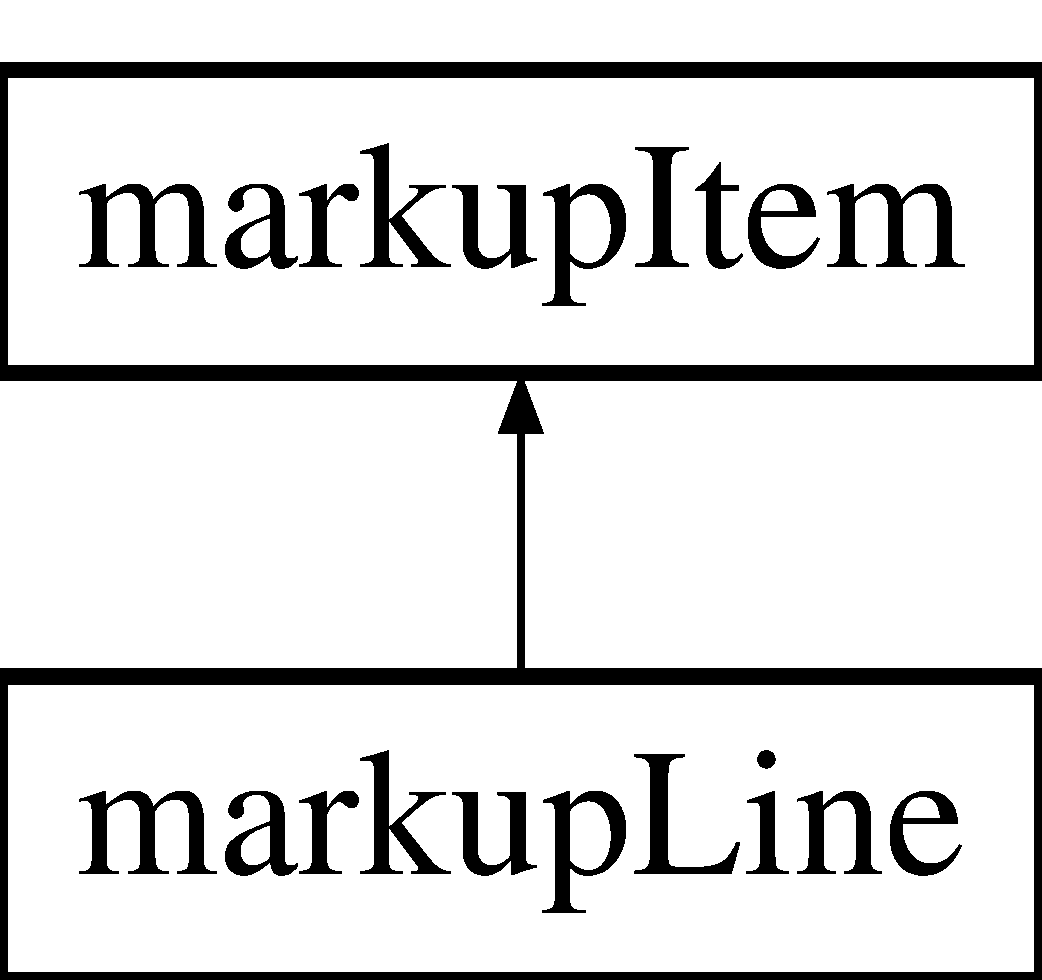
\includegraphics[height=2.000000cm]{classmarkupLine}
\end{center}
\end{figure}
\subsection*{Public Member Functions}
\begin{DoxyCompactItemize}
\item 
\hypertarget{classmarkupLine_a7a95e10ba3e4bda75e0c260ee6f95bd6}{
{\bfseries markupLine} (\hyperlink{classimageMarkup}{imageMarkup} $\ast$ownerIn, const bool interactiveIn, const bool reportOnMoveIn, const QString legendIn)}
\label{classmarkupLine_a7a95e10ba3e4bda75e0c260ee6f95bd6}

\item 
\hypertarget{classmarkupLine_a8164baa9961994148a13913a5186e711}{
void {\bfseries startDrawing} (const QPoint pos)}
\label{classmarkupLine_a8164baa9961994148a13913a5186e711}

\item 
\hypertarget{classmarkupLine_ac9999d4b2b96dd27cb05dc91d5211f86}{
void {\bfseries setArea} ()}
\label{classmarkupLine_ac9999d4b2b96dd27cb05dc91d5211f86}

\item 
\hypertarget{classmarkupLine_a923b6fc4a18acfcd883f24f38ca07119}{
void {\bfseries drawMarkup} (QPainter \&p)}
\label{classmarkupLine_a923b6fc4a18acfcd883f24f38ca07119}

\item 
\hypertarget{classmarkupLine_a939e2c560f454796212f0fceea50d387}{
void {\bfseries moveTo} (const QPoint pos)}
\label{classmarkupLine_a939e2c560f454796212f0fceea50d387}

\item 
\hypertarget{classmarkupLine_a76abf1570968523b650b9fd4f94cc9ff}{
bool {\bfseries isOver} (const QPoint point, QCursor $\ast$cursor)}
\label{classmarkupLine_a76abf1570968523b650b9fd4f94cc9ff}

\item 
\hypertarget{classmarkupLine_a2167abf14c5eba07ceb0041fe688fb7b}{
QPoint {\bfseries origin} ()}
\label{classmarkupLine_a2167abf14c5eba07ceb0041fe688fb7b}

\item 
\hypertarget{classmarkupLine_ad2fc7a98e9f20c7e532128d3f9d1f262}{
QCursor {\bfseries cursorForHandle} (const markupItem::markupHandles handle)}
\label{classmarkupLine_ad2fc7a98e9f20c7e532128d3f9d1f262}

\item 
\hypertarget{classmarkupLine_a22d3223e43b1fa36745d3b5febcda12c}{
QPoint {\bfseries getPoint1} ()}
\label{classmarkupLine_a22d3223e43b1fa36745d3b5febcda12c}

\item 
\hypertarget{classmarkupLine_a9b73e9f256d6661a97a51b0f17ea532b}{
QPoint {\bfseries getPoint2} ()}
\label{classmarkupLine_a9b73e9f256d6661a97a51b0f17ea532b}

\item 
\hypertarget{classmarkupLine_ad7e1dd31f002bf61d641de9f976477dc}{
unsigned int {\bfseries getThickness} ()}
\label{classmarkupLine_ad7e1dd31f002bf61d641de9f976477dc}

\item 
\hypertarget{classmarkupLine_aa387941af23d477813642f4dbcd67351}{
void {\bfseries setThickness} (const unsigned int thicknessIn)}
\label{classmarkupLine_aa387941af23d477813642f4dbcd67351}

\item 
\hypertarget{classmarkupLine_a2ee805b61113dafe417a1be248abcccd}{
QCursor {\bfseries defaultCursor} ()}
\label{classmarkupLine_a2ee805b61113dafe417a1be248abcccd}

\item 
\hypertarget{classmarkupLine_ae46565aa45cc6141b4efe70b6b0d74a8}{
void {\bfseries scaleSpecific} (const double xScale, const double yScale, const double zoomScale)}
\label{classmarkupLine_ae46565aa45cc6141b4efe70b6b0d74a8}

\end{DoxyCompactItemize}


The documentation for this class was generated from the following files:\begin{DoxyCompactItemize}
\item 
/tmp/epicsqt/trunk/framework/widgets/QEImage/imageMarkup.h\item 
/tmp/epicsqt/trunk/framework/widgets/QEImage/imageMarkup.cpp\end{DoxyCompactItemize}

\hypertarget{classmarkupRegion}{
\section{markupRegion Class Reference}
\label{classmarkupRegion}\index{markupRegion@{markupRegion}}
}
Inheritance diagram for markupRegion:\begin{figure}[H]
\begin{center}
\leavevmode
\includegraphics[height=2.000000cm]{classmarkupRegion}
\end{center}
\end{figure}
\subsection*{Public Member Functions}
\begin{DoxyCompactItemize}
\item 
\hypertarget{classmarkupRegion_ac73302b4f9f70b7430e31289ab8fa41b}{
{\bfseries markupRegion} (\hyperlink{classimageMarkup}{imageMarkup} $\ast$ownerIn, const bool interactiveIn, const bool reportOnMoveIn, const QString legendIn)}
\label{classmarkupRegion_ac73302b4f9f70b7430e31289ab8fa41b}

\item 
\hypertarget{classmarkupRegion_aced9ad7afa561e1a20f2313a663282e1}{
void {\bfseries startDrawing} (const QPoint pos)}
\label{classmarkupRegion_aced9ad7afa561e1a20f2313a663282e1}

\item 
\hypertarget{classmarkupRegion_ab190683626c279231fd8eb968b4db544}{
void {\bfseries setArea} ()}
\label{classmarkupRegion_ab190683626c279231fd8eb968b4db544}

\item 
\hypertarget{classmarkupRegion_abf847543e5dd7a6dffb62fa83fa90c8f}{
void {\bfseries drawMarkup} (QPainter \&p)}
\label{classmarkupRegion_abf847543e5dd7a6dffb62fa83fa90c8f}

\item 
\hypertarget{classmarkupRegion_a753ebf156c8cd56ff7e3edc5bf70bab8}{
void {\bfseries moveTo} (const QPoint pos)}
\label{classmarkupRegion_a753ebf156c8cd56ff7e3edc5bf70bab8}

\item 
\hypertarget{classmarkupRegion_a724084202aaedd367c70b5e165183452}{
bool {\bfseries isOver} (const QPoint point, QCursor $\ast$cursor)}
\label{classmarkupRegion_a724084202aaedd367c70b5e165183452}

\item 
\hypertarget{classmarkupRegion_a49c338512f240a3230a1ed2502345064}{
QPoint {\bfseries origin} ()}
\label{classmarkupRegion_a49c338512f240a3230a1ed2502345064}

\item 
\hypertarget{classmarkupRegion_aa7f1bb5ed6324fcc618afe06049ebc81}{
QCursor {\bfseries cursorForHandle} (const markupItem::markupHandles handle)}
\label{classmarkupRegion_aa7f1bb5ed6324fcc618afe06049ebc81}

\item 
\hypertarget{classmarkupRegion_a92d60ad5f5e87b5e23d0344afdc6dbb7}{
QPoint {\bfseries getPoint1} ()}
\label{classmarkupRegion_a92d60ad5f5e87b5e23d0344afdc6dbb7}

\item 
\hypertarget{classmarkupRegion_afd6e69f6ba9e223e3c520076606f7c76}{
QPoint {\bfseries getPoint2} ()}
\label{classmarkupRegion_afd6e69f6ba9e223e3c520076606f7c76}

\item 
\hypertarget{classmarkupRegion_a5743c9267044bf11b5d9471e1c5c6a12}{
unsigned int {\bfseries getThickness} ()}
\label{classmarkupRegion_a5743c9267044bf11b5d9471e1c5c6a12}

\item 
\hypertarget{classmarkupRegion_a0b33e9657e4f29af94bd8dcd595f8910}{
void {\bfseries setThickness} (const unsigned int thicknessIn)}
\label{classmarkupRegion_a0b33e9657e4f29af94bd8dcd595f8910}

\item 
\hypertarget{classmarkupRegion_ac54ee25b778827e637abd32bae344124}{
QCursor {\bfseries defaultCursor} ()}
\label{classmarkupRegion_ac54ee25b778827e637abd32bae344124}

\item 
\hypertarget{classmarkupRegion_a5ecf5a3727d916d21afcdc83ffe5c140}{
void {\bfseries scaleSpecific} (const double xScale, const double yScale, const double zoomScale)}
\label{classmarkupRegion_a5ecf5a3727d916d21afcdc83ffe5c140}

\item 
\hypertarget{classmarkupRegion_a7d4787f3f426ff54d49696aee6d2dd9f}{
void {\bfseries nonInteractiveUpdate} (QRect)}
\label{classmarkupRegion_a7d4787f3f426ff54d49696aee6d2dd9f}

\end{DoxyCompactItemize}


The documentation for this class was generated from the following files:\begin{DoxyCompactItemize}
\item 
/tmp/epicsqt/trunk/framework/widgets/QEImage/imageMarkup.h\item 
/tmp/epicsqt/trunk/framework/widgets/QEImage/imageMarkup.cpp\end{DoxyCompactItemize}

\hypertarget{classmarkupTarget}{
\section{markupTarget Class Reference}
\label{classmarkupTarget}\index{markupTarget@{markupTarget}}
}
Inheritance diagram for markupTarget:\begin{figure}[H]
\begin{center}
\leavevmode
\includegraphics[height=2.000000cm]{classmarkupTarget}
\end{center}
\end{figure}
\subsection*{Public Member Functions}
\begin{DoxyCompactItemize}
\item 
\hypertarget{classmarkupTarget_ad3480eb31ea67d4469c550363bf56146}{
{\bfseries markupTarget} (\hyperlink{classimageMarkup}{imageMarkup} $\ast$ownerIn, const bool interactiveIn, const bool reportOnMoveIn, const QString legendIn)}
\label{classmarkupTarget_ad3480eb31ea67d4469c550363bf56146}

\item 
\hypertarget{classmarkupTarget_affa4280c71754c2b7c103b29325eb661}{
void {\bfseries startDrawing} (const QPoint pos)}
\label{classmarkupTarget_affa4280c71754c2b7c103b29325eb661}

\item 
\hypertarget{classmarkupTarget_a14e4eb2ccb3d466c9e01aa54e79d1261}{
void {\bfseries setArea} ()}
\label{classmarkupTarget_a14e4eb2ccb3d466c9e01aa54e79d1261}

\item 
\hypertarget{classmarkupTarget_ad266b53ab93d38cbb713ccf0036e5ae2}{
void {\bfseries drawMarkup} (QPainter \&p)}
\label{classmarkupTarget_ad266b53ab93d38cbb713ccf0036e5ae2}

\item 
\hypertarget{classmarkupTarget_a24a4d8eaee3de1c740bf01d70facd509}{
void {\bfseries moveTo} (const QPoint pos)}
\label{classmarkupTarget_a24a4d8eaee3de1c740bf01d70facd509}

\item 
\hypertarget{classmarkupTarget_a58b8c80bc2f1eb7a02128559e0b98393}{
bool {\bfseries isOver} (const QPoint point, QCursor $\ast$cursor)}
\label{classmarkupTarget_a58b8c80bc2f1eb7a02128559e0b98393}

\item 
\hypertarget{classmarkupTarget_ade04074ff72727dcad49232e5061be49}{
QPoint {\bfseries origin} ()}
\label{classmarkupTarget_ade04074ff72727dcad49232e5061be49}

\item 
\hypertarget{classmarkupTarget_a6b2b40319837264553c878bac3f65c3a}{
QCursor {\bfseries cursorForHandle} (const markupItem::markupHandles handle)}
\label{classmarkupTarget_a6b2b40319837264553c878bac3f65c3a}

\item 
\hypertarget{classmarkupTarget_a28ef1e83cefc656c79ac1adbdac2e0c6}{
QPoint {\bfseries getPoint1} ()}
\label{classmarkupTarget_a28ef1e83cefc656c79ac1adbdac2e0c6}

\item 
\hypertarget{classmarkupTarget_a11183bfd70670de5c47f68b49a27c263}{
QPoint {\bfseries getPoint2} ()}
\label{classmarkupTarget_a11183bfd70670de5c47f68b49a27c263}

\item 
\hypertarget{classmarkupTarget_a0e1ccd644b853568b20c33afabd0b318}{
unsigned int {\bfseries getThickness} ()}
\label{classmarkupTarget_a0e1ccd644b853568b20c33afabd0b318}

\item 
\hypertarget{classmarkupTarget_a67888ae75a085edda05a1324498e8559}{
void {\bfseries setThickness} (const unsigned int thicknessIn)}
\label{classmarkupTarget_a67888ae75a085edda05a1324498e8559}

\item 
\hypertarget{classmarkupTarget_af02852e493c9470f94240ed80027c752}{
QCursor {\bfseries defaultCursor} ()}
\label{classmarkupTarget_af02852e493c9470f94240ed80027c752}

\item 
\hypertarget{classmarkupTarget_a557cafc31fac39d5be8a825abc793a00}{
void {\bfseries scaleSpecific} (const double xScale, const double yScale, const double zoomScale)}
\label{classmarkupTarget_a557cafc31fac39d5be8a825abc793a00}

\end{DoxyCompactItemize}


The documentation for this class was generated from the following files:\begin{DoxyCompactItemize}
\item 
/tmp/epicsqt/trunk/framework/widgets/QEImage/imageMarkup.h\item 
/tmp/epicsqt/trunk/framework/widgets/QEImage/imageMarkup.cpp\end{DoxyCompactItemize}

\hypertarget{classmarkupText}{
\section{markupText Class Reference}
\label{classmarkupText}\index{markupText@{markupText}}
}
Inheritance diagram for markupText:\begin{figure}[H]
\begin{center}
\leavevmode
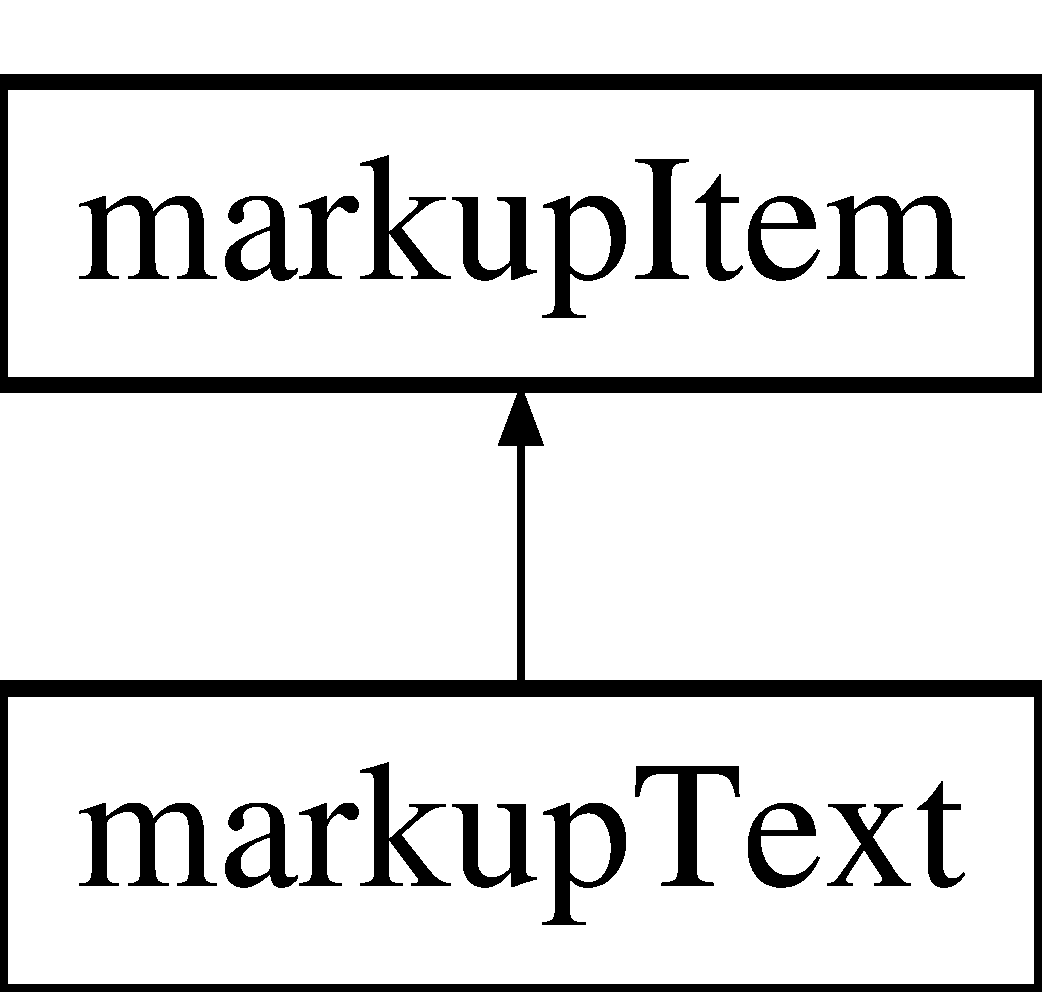
\includegraphics[height=2.000000cm]{classmarkupText}
\end{center}
\end{figure}
\subsection*{Public Member Functions}
\begin{DoxyCompactItemize}
\item 
\hypertarget{classmarkupText_ab10f4390437f296224ebc9227363e775}{
{\bfseries markupText} (\hyperlink{classimageMarkup}{imageMarkup} $\ast$ownerIn, const bool interactiveIn, const bool reportOnMoveIn, const QString legendIn)}
\label{classmarkupText_ab10f4390437f296224ebc9227363e775}

\item 
\hypertarget{classmarkupText_af93858c8d0f6af731c012bdef3e9d194}{
void {\bfseries setText} (QString textIn, bool draw)}
\label{classmarkupText_af93858c8d0f6af731c012bdef3e9d194}

\item 
\hypertarget{classmarkupText_a5644687c841f6eb1c844a13040d2453a}{
void {\bfseries startDrawing} (const QPoint pos)}
\label{classmarkupText_a5644687c841f6eb1c844a13040d2453a}

\item 
\hypertarget{classmarkupText_a3c64d2d513ef18ce32466ad03accdc12}{
void {\bfseries setArea} ()}
\label{classmarkupText_a3c64d2d513ef18ce32466ad03accdc12}

\item 
\hypertarget{classmarkupText_abcce7825fe6e9d6b5287ac7b402d785f}{
void {\bfseries drawMarkup} (QPainter \&p)}
\label{classmarkupText_abcce7825fe6e9d6b5287ac7b402d785f}

\item 
\hypertarget{classmarkupText_a9e8c68e748504328598220b9483d443c}{
void {\bfseries moveTo} (const QPoint pos)}
\label{classmarkupText_a9e8c68e748504328598220b9483d443c}

\item 
\hypertarget{classmarkupText_af64454b92fa176a8b7b2e7b1e8e6fb94}{
bool {\bfseries isOver} (const QPoint point, QCursor $\ast$cursor)}
\label{classmarkupText_af64454b92fa176a8b7b2e7b1e8e6fb94}

\item 
\hypertarget{classmarkupText_ae883f3edcba6a3c70bbabaf9ba1ebc5e}{
QPoint {\bfseries origin} ()}
\label{classmarkupText_ae883f3edcba6a3c70bbabaf9ba1ebc5e}

\item 
\hypertarget{classmarkupText_aaf88bc3f975bea3d3cbc2e04a78dd9cb}{
QCursor {\bfseries cursorForHandle} (const markupItem::markupHandles handle)}
\label{classmarkupText_aaf88bc3f975bea3d3cbc2e04a78dd9cb}

\item 
\hypertarget{classmarkupText_a0e1056c41ac8465a0d6257c2b17192bd}{
QPoint {\bfseries getPoint1} ()}
\label{classmarkupText_a0e1056c41ac8465a0d6257c2b17192bd}

\item 
\hypertarget{classmarkupText_aadcefe65b8d559e50d3ce7c3111b8ee0}{
QPoint {\bfseries getPoint2} ()}
\label{classmarkupText_aadcefe65b8d559e50d3ce7c3111b8ee0}

\item 
\hypertarget{classmarkupText_a927a0d805ff4c8161db72d645f4c0189}{
unsigned int {\bfseries getThickness} ()}
\label{classmarkupText_a927a0d805ff4c8161db72d645f4c0189}

\item 
\hypertarget{classmarkupText_a0dac42dcf535cbb3789d1d85c0533154}{
void {\bfseries setThickness} (const unsigned int thicknessIn)}
\label{classmarkupText_a0dac42dcf535cbb3789d1d85c0533154}

\item 
\hypertarget{classmarkupText_aaac3cc8458c9d760fe671d8bd8e06fc1}{
QCursor {\bfseries defaultCursor} ()}
\label{classmarkupText_aaac3cc8458c9d760fe671d8bd8e06fc1}

\item 
\hypertarget{classmarkupText_aa6ce0350b7e119353e35d1bf865b3741}{
void {\bfseries scaleSpecific} (const double xScale, const double yScale, const double zoomScale)}
\label{classmarkupText_aa6ce0350b7e119353e35d1bf865b3741}

\end{DoxyCompactItemize}


The documentation for this class was generated from the following files:\begin{DoxyCompactItemize}
\item 
/tmp/epicsqt/trunk/framework/widgets/QEImage/imageMarkup.h\item 
/tmp/epicsqt/trunk/framework/widgets/QEImage/imageMarkup.cpp\end{DoxyCompactItemize}

\hypertarget{classmarkupVLine}{
\section{markupVLine Class Reference}
\label{classmarkupVLine}\index{markupVLine@{markupVLine}}
}
Inheritance diagram for markupVLine:\begin{figure}[H]
\begin{center}
\leavevmode
\includegraphics[height=2.000000cm]{classmarkupVLine}
\end{center}
\end{figure}
\subsection*{Public Member Functions}
\begin{DoxyCompactItemize}
\item 
\hypertarget{classmarkupVLine_a80f4f99affe9283b446df869653c97fb}{
{\bfseries markupVLine} (\hyperlink{classimageMarkup}{imageMarkup} $\ast$ownerIn, const bool interactiveIn, const bool reportOnMoveIn, const QString legendIn)}
\label{classmarkupVLine_a80f4f99affe9283b446df869653c97fb}

\item 
\hypertarget{classmarkupVLine_a66fc9bf5d533eb1665706ebe94b9d0f4}{
void {\bfseries startDrawing} (const QPoint pos)}
\label{classmarkupVLine_a66fc9bf5d533eb1665706ebe94b9d0f4}

\item 
\hypertarget{classmarkupVLine_adafd13c9dd29d233da521c9a9af14069}{
void {\bfseries setArea} ()}
\label{classmarkupVLine_adafd13c9dd29d233da521c9a9af14069}

\item 
void \hyperlink{classmarkupVLine_af472c2fb30fa50d178f3ded4f9191501}{drawMarkup} (QPainter \&p)
\item 
\hypertarget{classmarkupVLine_a43293f707098584cca7342353d5ac7bc}{
void {\bfseries moveTo} (const QPoint pos)}
\label{classmarkupVLine_a43293f707098584cca7342353d5ac7bc}

\item 
\hypertarget{classmarkupVLine_a65e90b752c08aa71c287004e2d7e0a53}{
bool {\bfseries isOver} (const QPoint point, QCursor $\ast$cursor)}
\label{classmarkupVLine_a65e90b752c08aa71c287004e2d7e0a53}

\item 
\hypertarget{classmarkupVLine_ac67fe2d2b7768cfb6836682ef517e421}{
QPoint {\bfseries origin} ()}
\label{classmarkupVLine_ac67fe2d2b7768cfb6836682ef517e421}

\item 
\hypertarget{classmarkupVLine_a197cf853a40951660dd35706070808b9}{
QCursor {\bfseries cursorForHandle} (const markupItem::markupHandles handle)}
\label{classmarkupVLine_a197cf853a40951660dd35706070808b9}

\item 
\hypertarget{classmarkupVLine_ab5c9a3ee21f4503d5aa0126fc1b02dca}{
QPoint {\bfseries getPoint1} ()}
\label{classmarkupVLine_ab5c9a3ee21f4503d5aa0126fc1b02dca}

\item 
\hypertarget{classmarkupVLine_a5119650e1e929020eaf5b12e42a93866}{
QPoint {\bfseries getPoint2} ()}
\label{classmarkupVLine_a5119650e1e929020eaf5b12e42a93866}

\item 
\hypertarget{classmarkupVLine_a739499cfdd4d7108d0e8720f6f698639}{
unsigned int {\bfseries getThickness} ()}
\label{classmarkupVLine_a739499cfdd4d7108d0e8720f6f698639}

\item 
\hypertarget{classmarkupVLine_a4d68fa70410edda731a334c5a8fc9f51}{
void {\bfseries setThickness} (const unsigned int thicknessIn)}
\label{classmarkupVLine_a4d68fa70410edda731a334c5a8fc9f51}

\item 
\hypertarget{classmarkupVLine_ab6470c361db7d579a05fd9bd2e1c6942}{
QCursor {\bfseries defaultCursor} ()}
\label{classmarkupVLine_ab6470c361db7d579a05fd9bd2e1c6942}

\item 
\hypertarget{classmarkupVLine_a2e2752be3227116e9811544e249cb3ca}{
void {\bfseries scaleSpecific} (const double xScale, const double yScale, const double zoomScale)}
\label{classmarkupVLine_a2e2752be3227116e9811544e249cb3ca}

\end{DoxyCompactItemize}


\subsection{Member Function Documentation}
\hypertarget{classmarkupVLine_af472c2fb30fa50d178f3ded4f9191501}{
\index{markupVLine@{markupVLine}!drawMarkup@{drawMarkup}}
\index{drawMarkup@{drawMarkup}!markupVLine@{markupVLine}}
\subsubsection[{drawMarkup}]{\setlength{\rightskip}{0pt plus 5cm}void markupVLine::drawMarkup (
\begin{DoxyParamCaption}
\item[{QPainter \&}]{p}
\end{DoxyParamCaption}
)\hspace{0.3cm}{\ttfamily  \mbox{[}virtual\mbox{]}}}}
\label{classmarkupVLine_af472c2fb30fa50d178f3ded4f9191501}


!! draw the handle in the middle of the existing view, not the entire image 



Implements \hyperlink{classmarkupItem}{markupItem}.



The documentation for this class was generated from the following files:\begin{DoxyCompactItemize}
\item 
/tmp/epicsqt/trunk/framework/widgets/QEImage/imageMarkup.h\item 
/tmp/epicsqt/trunk/framework/widgets/QEImage/imageMarkup.cpp\end{DoxyCompactItemize}

\hypertarget{classmessage__types}{
\section{message\_\-types Class Reference}
\label{classmessage__types}\index{message\_\-types@{message\_\-types}}
}
\subsection*{Public Member Functions}
\begin{DoxyCompactItemize}
\item 
\hypertarget{classmessage__types_a2014b738fdf5f7a84561b2837fb5da1f}{
{\bfseries message\_\-types} (message\_\-severities severityIn, message\_\-kind\_\-sets kind\_\-setIn=MESSAGE\_\-KIND\_\-STANDARD)}
\label{classmessage__types_a2014b738fdf5f7a84561b2837fb5da1f}

\item 
\hypertarget{classmessage__types_a07f6deb90c205ac15514b6ccdebc007d}{
QString \hyperlink{classmessage__types_a07f6deb90c205ac15514b6ccdebc007d}{getSeverityName} ()}
\label{classmessage__types_a07f6deb90c205ac15514b6ccdebc007d}

\begin{DoxyCompactList}\small\item\em Function to provide string name for each message type severity. \end{DoxyCompactList}\end{DoxyCompactItemize}
\subsection*{Public Attributes}
\begin{DoxyCompactItemize}
\item 
\hypertarget{classmessage__types_a0b8f4af672670a810e90dc66a883b9c8}{
message\_\-severities {\bfseries severity}}
\label{classmessage__types_a0b8f4af672670a810e90dc66a883b9c8}

\item 
\hypertarget{classmessage__types_a7967011affb00d6db2d9b0e4842ba0ef}{
message\_\-kind\_\-sets {\bfseries kind\_\-set}}
\label{classmessage__types_a7967011affb00d6db2d9b0e4842ba0ef}

\end{DoxyCompactItemize}


The documentation for this class was generated from the following files:\begin{DoxyCompactItemize}
\item 
/tmp/epicsqt/trunk/framework/widgets/include/UserMessage.h\item 
/tmp/epicsqt/trunk/framework/widgets/src/UserMessage.cpp\end{DoxyCompactItemize}

\hypertarget{classQEStripChartToolBar_1_1OwnWidgets}{
\section{QEStripChartToolBar::OwnWidgets Class Reference}
\label{classQEStripChartToolBar_1_1OwnWidgets}\index{QEStripChartToolBar::OwnWidgets@{QEStripChartToolBar::OwnWidgets}}
}
\subsection*{Public Member Functions}
\begin{DoxyCompactItemize}
\item 
\hypertarget{classQEStripChartToolBar_1_1OwnWidgets_aeee71859e97c5618ca82d9b94c1a9974}{
{\bfseries OwnWidgets} (\hyperlink{classQEStripChartToolBar}{QEStripChartToolBar} $\ast$parent)}
\label{classQEStripChartToolBar_1_1OwnWidgets_aeee71859e97c5618ca82d9b94c1a9974}

\end{DoxyCompactItemize}
\subsection*{Public Attributes}
\begin{DoxyCompactItemize}
\item 
\hypertarget{classQEStripChartToolBar_1_1OwnWidgets_a41b4f4bc025beaeb9146a44638ebc5c6}{
QPushButton $\ast$ {\bfseries pushButtons} \mbox{[}NUMBER\_\-OF\_\-BUTTONS\mbox{]}}
\label{classQEStripChartToolBar_1_1OwnWidgets_a41b4f4bc025beaeb9146a44638ebc5c6}

\item 
\hypertarget{classQEStripChartToolBar_1_1OwnWidgets_a6a3ce5d64435364f376c127adfdd72e5}{
QLabel $\ast$ {\bfseries timeStatus}}
\label{classQEStripChartToolBar_1_1OwnWidgets_a6a3ce5d64435364f376c127adfdd72e5}

\end{DoxyCompactItemize}


The documentation for this class was generated from the following file:\begin{DoxyCompactItemize}
\item 
/tmp/epicsqt/trunk/framework/widgets/QEStripChart/QEStripChartToolBar.cpp\end{DoxyCompactItemize}

\hypertarget{classQEPvProperties_1_1OwnWidgets}{
\section{QEPvProperties::OwnWidgets Class Reference}
\label{classQEPvProperties_1_1OwnWidgets}\index{QEPvProperties::OwnWidgets@{QEPvProperties::OwnWidgets}}
}
\subsection*{Public Member Functions}
\begin{DoxyCompactItemize}
\item 
\hypertarget{classQEPvProperties_1_1OwnWidgets_ad40480cd4a09f4b275c5c41520d6cb40}{
{\bfseries OwnWidgets} (\hyperlink{classQEPvProperties}{QEPvProperties} $\ast$parent)}
\label{classQEPvProperties_1_1OwnWidgets_ad40480cd4a09f4b275c5c41520d6cb40}

\end{DoxyCompactItemize}
\subsection*{Public Attributes}
\begin{DoxyCompactItemize}
\item 
\hypertarget{classQEPvProperties_1_1OwnWidgets_a1ecec9d99ec1a3e9c4e57231e78e4135}{
QFrame $\ast$ {\bfseries topFrame}}
\label{classQEPvProperties_1_1OwnWidgets_a1ecec9d99ec1a3e9c4e57231e78e4135}

\item 
\hypertarget{classQEPvProperties_1_1OwnWidgets_af6e8e658553d902e4d0c0e1fdef22416}{
QLabel $\ast$ {\bfseries label1}}
\label{classQEPvProperties_1_1OwnWidgets_af6e8e658553d902e4d0c0e1fdef22416}

\item 
\hypertarget{classQEPvProperties_1_1OwnWidgets_a39bee02c2e3a90401edfdb884baf72dc}{
QLabel $\ast$ {\bfseries label2}}
\label{classQEPvProperties_1_1OwnWidgets_a39bee02c2e3a90401edfdb884baf72dc}

\item 
\hypertarget{classQEPvProperties_1_1OwnWidgets_a34bdb1bf97c0027ef7d3cdbcc9dc6a40}{
QLabel $\ast$ {\bfseries label3}}
\label{classQEPvProperties_1_1OwnWidgets_a34bdb1bf97c0027ef7d3cdbcc9dc6a40}

\item 
\hypertarget{classQEPvProperties_1_1OwnWidgets_a6e38f5e2da6a392724659493e61f127b}{
QLabel $\ast$ {\bfseries label4}}
\label{classQEPvProperties_1_1OwnWidgets_a6e38f5e2da6a392724659493e61f127b}

\item 
\hypertarget{classQEPvProperties_1_1OwnWidgets_a5a8421c1903aa58acfe23106a8e6aabc}{
QLabel $\ast$ {\bfseries label5}}
\label{classQEPvProperties_1_1OwnWidgets_a5a8421c1903aa58acfe23106a8e6aabc}

\item 
\hypertarget{classQEPvProperties_1_1OwnWidgets_a387ed7e1f879dfb46aad77482a32e140}{
QLabel $\ast$ {\bfseries label6}}
\label{classQEPvProperties_1_1OwnWidgets_a387ed7e1f879dfb46aad77482a32e140}

\item 
\hypertarget{classQEPvProperties_1_1OwnWidgets_a35e72a3cf22930f6172f6ebf2ae51c8c}{
QComboBox $\ast$ {\bfseries box}}
\label{classQEPvProperties_1_1OwnWidgets_a35e72a3cf22930f6172f6ebf2ae51c8c}

\item 
\hypertarget{classQEPvProperties_1_1OwnWidgets_a47455c8d0cdc74e0c7c20fabaebd4624}{
\hyperlink{classQELabel}{QELabel} $\ast$ {\bfseries valueLabel}}
\label{classQEPvProperties_1_1OwnWidgets_a47455c8d0cdc74e0c7c20fabaebd4624}

\item 
\hypertarget{classQEPvProperties_1_1OwnWidgets_ac55392b52a856d7f3266e7c335407159}{
QLabel $\ast$ {\bfseries hostName}}
\label{classQEPvProperties_1_1OwnWidgets_ac55392b52a856d7f3266e7c335407159}

\item 
\hypertarget{classQEPvProperties_1_1OwnWidgets_a88b24dcc3898a10fbbd10d77ff022443}{
QLabel $\ast$ {\bfseries fieldType}}
\label{classQEPvProperties_1_1OwnWidgets_a88b24dcc3898a10fbbd10d77ff022443}

\item 
\hypertarget{classQEPvProperties_1_1OwnWidgets_aeb19416771f319e93e700c63b0974240}{
QLabel $\ast$ {\bfseries timeStamp}}
\label{classQEPvProperties_1_1OwnWidgets_aeb19416771f319e93e700c63b0974240}

\item 
\hypertarget{classQEPvProperties_1_1OwnWidgets_ab34f2804bfbeb686246bb345472f192f}{
QLabel $\ast$ {\bfseries indexInfo}}
\label{classQEPvProperties_1_1OwnWidgets_ab34f2804bfbeb686246bb345472f192f}

\item 
\hypertarget{classQEPvProperties_1_1OwnWidgets_a962d4bd4d2bd23a45423d2ac6bdbe398}{
QVBoxLayout $\ast$ {\bfseries topFrameVlayout}}
\label{classQEPvProperties_1_1OwnWidgets_a962d4bd4d2bd23a45423d2ac6bdbe398}

\item 
\hypertarget{classQEPvProperties_1_1OwnWidgets_ac366d8bbfac62bdb60ff38d0463cd9c9}{
QHBoxLayout $\ast$ {\bfseries hlayouts} \mbox{[}6\mbox{]}}
\label{classQEPvProperties_1_1OwnWidgets_ac366d8bbfac62bdb60ff38d0463cd9c9}

\item 
\hypertarget{classQEPvProperties_1_1OwnWidgets_acbc6d7dd9d0048eab134df7ae0ed0781}{
QTableWidget $\ast$ {\bfseries table}}
\label{classQEPvProperties_1_1OwnWidgets_acbc6d7dd9d0048eab134df7ae0ed0781}

\item 
\hypertarget{classQEPvProperties_1_1OwnWidgets_ab0654db63825be1d26d6947be3869126}{
QMenu $\ast$ {\bfseries tableContextMenu}}
\label{classQEPvProperties_1_1OwnWidgets_ab0654db63825be1d26d6947be3869126}

\item 
\hypertarget{classQEPvProperties_1_1OwnWidgets_abd19ede617948cdda206c017ff68462b}{
QFrame $\ast$ {\bfseries enumerationFrame}}
\label{classQEPvProperties_1_1OwnWidgets_abd19ede617948cdda206c017ff68462b}

\item 
\hypertarget{classQEPvProperties_1_1OwnWidgets_aa15a994836c1365fabee4a946b9f2213}{
\hyperlink{classQLabelList}{QLabelList} {\bfseries enumerationLabelList}}
\label{classQEPvProperties_1_1OwnWidgets_aa15a994836c1365fabee4a946b9f2213}

\item 
\hypertarget{classQEPvProperties_1_1OwnWidgets_a57eddf3bc725bbb54bbca2f18dc398d0}{
QScrollArea $\ast$ {\bfseries enumerationScroll}}
\label{classQEPvProperties_1_1OwnWidgets_a57eddf3bc725bbb54bbca2f18dc398d0}

\item 
\hypertarget{classQEPvProperties_1_1OwnWidgets_a4dd09384598daee724bf518fbe2acad9}{
QEResizeableFrame $\ast$ {\bfseries enumerationResize}}
\label{classQEPvProperties_1_1OwnWidgets_a4dd09384598daee724bf518fbe2acad9}

\item 
\hypertarget{classQEPvProperties_1_1OwnWidgets_aa538b1ebed199f7e062ededdb85baedb}{
QVBoxLayout $\ast$ {\bfseries vlayout}}
\label{classQEPvProperties_1_1OwnWidgets_aa538b1ebed199f7e062ededdb85baedb}

\end{DoxyCompactItemize}


The documentation for this class was generated from the following file:\begin{DoxyCompactItemize}
\item 
/tmp/epicsqt/trunk/framework/widgets/QEPvProperties/QEPvProperties.cpp\end{DoxyCompactItemize}

\hypertarget{classPeriodicDialog}{
\section{PeriodicDialog Class Reference}
\label{classPeriodicDialog}\index{PeriodicDialog@{PeriodicDialog}}
}
\subsection*{Public Member Functions}
\begin{DoxyCompactItemize}
\item 
\hypertarget{classPeriodicDialog_a0b80d1a3ee6bc4093443ace6df669a5f}{
{\bfseries PeriodicDialog} (QWidget $\ast$parent=0)}
\label{classPeriodicDialog_a0b80d1a3ee6bc4093443ace6df669a5f}

\item 
\hypertarget{classPeriodicDialog_a41537b40e44672d232ae40db67002a46}{
QString {\bfseries getElement} ()}
\label{classPeriodicDialog_a41537b40e44672d232ae40db67002a46}

\item 
\hypertarget{classPeriodicDialog_a91d6d64e65968baf3d79a8dd8a530520}{
void {\bfseries setElement} (QString elementIn, QList$<$ bool $>$ \&enabledList, QList$<$ QString $>$ \&elementList)}
\label{classPeriodicDialog_a91d6d64e65968baf3d79a8dd8a530520}

\end{DoxyCompactItemize}
\subsection*{Protected Member Functions}
\begin{DoxyCompactItemize}
\item 
\hypertarget{classPeriodicDialog_a19b89ad736f22b9bf27301878aa18c48}{
void {\bfseries changeEvent} (QEvent $\ast$e)}
\label{classPeriodicDialog_a19b89ad736f22b9bf27301878aa18c48}

\end{DoxyCompactItemize}


The documentation for this class was generated from the following files:\begin{DoxyCompactItemize}
\item 
/tmp/epicsqt/trunk/framework/widgets/QEPeriodic/PeriodicDialog.h\item 
/tmp/epicsqt/trunk/framework/widgets/QEPeriodic/PeriodicDialog.cpp\end{DoxyCompactItemize}

\hypertarget{classPeriodicElementSetupForm}{
\section{PeriodicElementSetupForm Class Reference}
\label{classPeriodicElementSetupForm}\index{PeriodicElementSetupForm@{PeriodicElementSetupForm}}
}
\subsection*{Public Member Functions}
\begin{DoxyCompactItemize}
\item 
\hypertarget{classPeriodicElementSetupForm_a940a28c6abe0e29568a9680f638fdd43}{
{\bfseries PeriodicElementSetupForm} (QWidget $\ast$parent=0)}
\label{classPeriodicElementSetupForm_a940a28c6abe0e29568a9680f638fdd43}

\end{DoxyCompactItemize}


The documentation for this class was generated from the following files:\begin{DoxyCompactItemize}
\item 
/tmp/epicsqt/trunk/framework/widgets/QEPeriodic/PeriodicElementSetupForm.h\item 
/tmp/epicsqt/trunk/framework/widgets/QEPeriodic/PeriodicElementSetupForm.cpp\end{DoxyCompactItemize}

\hypertarget{classPeriodicSetupDialog}{
\section{PeriodicSetupDialog Class Reference}
\label{classPeriodicSetupDialog}\index{PeriodicSetupDialog@{PeriodicSetupDialog}}
}
\subsection*{Public Member Functions}
\begin{DoxyCompactItemize}
\item 
\hypertarget{classPeriodicSetupDialog_a94edb9a86f6790d54813a8107617668f}{
{\bfseries PeriodicSetupDialog} (QWidget $\ast$parent=0)}
\label{classPeriodicSetupDialog_a94edb9a86f6790d54813a8107617668f}

\end{DoxyCompactItemize}


The documentation for this class was generated from the following files:\begin{DoxyCompactItemize}
\item 
/tmp/epicsqt/trunk/framework/widgets/QEPeriodic/PeriodicSetupDialog.h\item 
/tmp/epicsqt/trunk/framework/widgets/QEPeriodic/PeriodicSetupDialog.cpp\end{DoxyCompactItemize}

\hypertarget{classPersistanceManager}{
\section{PersistanceManager Class Reference}
\label{classPersistanceManager}\index{PersistanceManager@{PersistanceManager}}
}
\subsection*{Public Member Functions}
\begin{DoxyCompactItemize}
\item 
\hypertarget{classPersistanceManager_a610154c67ea20021e7d8e3f9275c0992}{
QObject $\ast$ {\bfseries getSaveRestoreObject} ()}
\label{classPersistanceManager_a610154c67ea20021e7d8e3f9275c0992}

\item 
\hypertarget{classPersistanceManager_a03a6dfbabd73201a52ebd125e4ab417e}{
void {\bfseries save} (const QString fileName, const QString rootName, const QString configName)}
\label{classPersistanceManager_a03a6dfbabd73201a52ebd125e4ab417e}

\item 
\hypertarget{classPersistanceManager_a3f4cb41b8bc6633e00fb1dcf58395c6b}{
void {\bfseries restore} (const QString fileName, const QString rootName, const QString configName)}
\label{classPersistanceManager_a3f4cb41b8bc6633e00fb1dcf58395c6b}

\item 
\hypertarget{classPersistanceManager_aba899c3429aad480bfef9cab420cb123}{
\hyperlink{classPMElement}{PMElement} {\bfseries addNamedConfiguration} (QString name)}
\label{classPersistanceManager_aba899c3429aad480bfef9cab420cb123}

\item 
\hypertarget{classPersistanceManager_a2625b70c4ea0e2b6fffda098c15dd5f4}{
\hyperlink{classPMElement}{PMElement} {\bfseries getNamedConfiguration} (QString name)}
\label{classPersistanceManager_a2625b70c4ea0e2b6fffda098c15dd5f4}

\item 
\hypertarget{classPersistanceManager_abb4df1e15f39379ffd3bbf86c4919648}{
QStringList {\bfseries getConfigNames} (QString fileName, QString rootName)}
\label{classPersistanceManager_abb4df1e15f39379ffd3bbf86c4919648}

\item 
\hypertarget{classPersistanceManager_a7f65f2aeb084529b3b1c1fe9928ce88b}{
void {\bfseries deleteConfigs} (QString fileName, QString rootName, QStringList names)}
\label{classPersistanceManager_a7f65f2aeb084529b3b1c1fe9928ce88b}

\end{DoxyCompactItemize}
\subsection*{Friends}
\begin{DoxyCompactItemize}
\item 
\hypertarget{classPersistanceManager_a9044d73aebbb01c7c72514c8ca06d590}{
class \hyperlink{classPersistanceManager_a9044d73aebbb01c7c72514c8ca06d590}{PMElement}}
\label{classPersistanceManager_a9044d73aebbb01c7c72514c8ca06d590}

\end{DoxyCompactItemize}


The documentation for this class was generated from the following files:\begin{DoxyCompactItemize}
\item 
/tmp/epicsqt/trunk/framework/widgets/include/persistanceManager.h\item 
/tmp/epicsqt/trunk/framework/widgets/src/persistanceManager.cpp\end{DoxyCompactItemize}

\hypertarget{classPMContext}{
\section{PMContext Class Reference}
\label{classPMContext}\index{PMContext@{PMContext}}
}


The documentation for this class was generated from the following file:\begin{DoxyCompactItemize}
\item 
/tmp/epicsqt/trunk/framework/widgets/include/persistanceManager.h\end{DoxyCompactItemize}

\hypertarget{classPMElement}{
\section{PMElement Class Reference}
\label{classPMElement}\index{PMElement@{PMElement}}
}
\subsection*{Public Member Functions}
\begin{DoxyCompactItemize}
\item 
\hypertarget{classPMElement_aaf767805374acfe4212530c6a68bea8f}{
{\bfseries PMElement} (\hyperlink{classPersistanceManager}{PersistanceManager} $\ast$ownerIn, QDomElement elementIn)}
\label{classPMElement_aaf767805374acfe4212530c6a68bea8f}

\item 
\hypertarget{classPMElement_a17a7cd68ecbca27fa58b0f69ed055387}{
\hyperlink{classPMElement}{PMElement} {\bfseries addElement} (QString name)}
\label{classPMElement_a17a7cd68ecbca27fa58b0f69ed055387}

\item 
\hypertarget{classPMElement_a876c0e281880fead7dbd75911a2c3e93}{
void {\bfseries addValue} (QString name, bool value)}
\label{classPMElement_a876c0e281880fead7dbd75911a2c3e93}

\item 
\hypertarget{classPMElement_a954974405145bd9a68961734b6742d65}{
void {\bfseries addValue} (QString name, int value)}
\label{classPMElement_a954974405145bd9a68961734b6742d65}

\item 
\hypertarget{classPMElement_a8ecb48a41bd01fc1b9685e51ad89aa83}{
void {\bfseries addValue} (QString name, double value)}
\label{classPMElement_a8ecb48a41bd01fc1b9685e51ad89aa83}

\item 
\hypertarget{classPMElement_a6a4ea26de47673b709864aa603212016}{
void {\bfseries addValue} (QString name, QString value)}
\label{classPMElement_a6a4ea26de47673b709864aa603212016}

\item 
\hypertarget{classPMElement_ada18dfe6db12c2452194024a7a73b479}{
void {\bfseries addAttribute} (QString name, bool value)}
\label{classPMElement_ada18dfe6db12c2452194024a7a73b479}

\item 
\hypertarget{classPMElement_aff235752a9d26313cd216eb15d1cd3b8}{
void {\bfseries addAttribute} (QString name, int value)}
\label{classPMElement_aff235752a9d26313cd216eb15d1cd3b8}

\item 
\hypertarget{classPMElement_a1f5a9f2813c475d50c0641f02218db73}{
void {\bfseries addAttribute} (QString name, double value)}
\label{classPMElement_a1f5a9f2813c475d50c0641f02218db73}

\item 
\hypertarget{classPMElement_ab02a2810666cc0644c370fe1cfa11533}{
void {\bfseries addAttribute} (QString name, QString value)}
\label{classPMElement_ab02a2810666cc0644c370fe1cfa11533}

\item 
\hypertarget{classPMElement_a9f8063f859988f5e93029a1d21f8882d}{
\hyperlink{classPMElement}{PMElement} {\bfseries getElement} (QString name)}
\label{classPMElement_a9f8063f859988f5e93029a1d21f8882d}

\item 
\hypertarget{classPMElement_a50e6b700a78be12a0ecd6e05af4880f3}{
\hyperlink{classPMElement}{PMElement} {\bfseries getElement} (QString name, int i)}
\label{classPMElement_a50e6b700a78be12a0ecd6e05af4880f3}

\item 
\hypertarget{classPMElement_affd4449d5a7fb0343a01b02c3026186a}{
\hyperlink{classPMElement}{PMElement} {\bfseries getElement} (QString name, QString attrName, QString attrValue)}
\label{classPMElement_affd4449d5a7fb0343a01b02c3026186a}

\item 
\hypertarget{classPMElement_a36440721ff4961e057adbee6dbe02a2e}{
\hyperlink{classPMElementList}{PMElementList} {\bfseries getElementList} (QString name)}
\label{classPMElement_a36440721ff4961e057adbee6dbe02a2e}

\item 
\hypertarget{classPMElement_ab181ab8d8db6e40dcc4d056deb637395}{
bool {\bfseries getValue} (QString name, bool \&val)}
\label{classPMElement_ab181ab8d8db6e40dcc4d056deb637395}

\item 
\hypertarget{classPMElement_a366d41cdb0194c6203cb66d06b03b93c}{
bool {\bfseries getValue} (QString name, int \&val)}
\label{classPMElement_a366d41cdb0194c6203cb66d06b03b93c}

\item 
\hypertarget{classPMElement_aaa0e58c65c9756abb0c330f069c56c4f}{
bool {\bfseries getValue} (QString name, double \&val)}
\label{classPMElement_aaa0e58c65c9756abb0c330f069c56c4f}

\item 
\hypertarget{classPMElement_ae39a1d735cceb85d71fadb4afa63be02}{
bool {\bfseries getValue} (QString name, QString \&val)}
\label{classPMElement_ae39a1d735cceb85d71fadb4afa63be02}

\item 
\hypertarget{classPMElement_a3aeee273dcfa62c36a94804d2d0be3a6}{
bool {\bfseries getAttribute} (QString name, bool \&val)}
\label{classPMElement_a3aeee273dcfa62c36a94804d2d0be3a6}

\item 
\hypertarget{classPMElement_a0957c8c16bc1fb6af400775576f8a2d9}{
bool {\bfseries getAttribute} (QString name, int \&val)}
\label{classPMElement_a0957c8c16bc1fb6af400775576f8a2d9}

\item 
\hypertarget{classPMElement_aab2c89af1d53fa4be12040ad4c83f6b2}{
bool {\bfseries getAttribute} (QString name, double \&val)}
\label{classPMElement_aab2c89af1d53fa4be12040ad4c83f6b2}

\item 
\hypertarget{classPMElement_a9da1b4466231bc98af036120847982e8}{
bool {\bfseries getAttribute} (QString name, QString \&val)}
\label{classPMElement_a9da1b4466231bc98af036120847982e8}

\item 
\hypertarget{classPMElement_acef70c97acb6e8403ddbf172c323fcdb}{
bool {\bfseries isNull} ()}
\label{classPMElement_acef70c97acb6e8403ddbf172c323fcdb}

\end{DoxyCompactItemize}


The documentation for this class was generated from the following files:\begin{DoxyCompactItemize}
\item 
/tmp/epicsqt/trunk/framework/widgets/include/persistanceManager.h\item 
/tmp/epicsqt/trunk/framework/widgets/src/persistanceManager.cpp\end{DoxyCompactItemize}

\hypertarget{classPMElementList}{
\section{PMElementList Class Reference}
\label{classPMElementList}\index{PMElementList@{PMElementList}}
}
\subsection*{Public Member Functions}
\begin{DoxyCompactItemize}
\item 
\hypertarget{classPMElementList_a8125d9dccfc0c0af6d371d9349aaefec}{
{\bfseries PMElementList} (\hyperlink{classPersistanceManager}{PersistanceManager} $\ast$ownerIn, QDomNodeList elementListIn)}
\label{classPMElementList_a8125d9dccfc0c0af6d371d9349aaefec}

\item 
\hyperlink{classPMElement}{PMElement} \hyperlink{classPMElementList_a4a4dcec6d88a6602b72e4c6d542fe4a4}{getElement} (int i)
\item 
\hypertarget{classPMElementList_ae353e85779a3753265b3b4ae7b82ee9c}{
int {\bfseries count} ()}
\label{classPMElementList_ae353e85779a3753265b3b4ae7b82ee9c}

\end{DoxyCompactItemize}


\subsection{Member Function Documentation}
\hypertarget{classPMElementList_a4a4dcec6d88a6602b72e4c6d542fe4a4}{
\index{PMElementList@{PMElementList}!getElement@{getElement}}
\index{getElement@{getElement}!PMElementList@{PMElementList}}
\subsubsection[{getElement}]{\setlength{\rightskip}{0pt plus 5cm}{\bf PMElement} PMElementList::getElement (
\begin{DoxyParamCaption}
\item[{int}]{i}
\end{DoxyParamCaption}
)}}
\label{classPMElementList_a4a4dcec6d88a6602b72e4c6d542fe4a4}


!! check range of i 



The documentation for this class was generated from the following files:\begin{DoxyCompactItemize}
\item 
/tmp/epicsqt/trunk/framework/widgets/include/persistanceManager.h\item 
/tmp/epicsqt/trunk/framework/widgets/src/persistanceManager.cpp\end{DoxyCompactItemize}

\hypertarget{classQEStripChart_1_1PrivateData}{
\section{QEStripChart::PrivateData Class Reference}
\label{classQEStripChart_1_1PrivateData}\index{QEStripChart::PrivateData@{QEStripChart::PrivateData}}
}
\subsection*{Public Member Functions}
\begin{DoxyCompactItemize}
\item 
\hypertarget{classQEStripChart_1_1PrivateData_a4d230180059f20db3b27701b13f2c548}{
{\bfseries PrivateData} (\hyperlink{classQEStripChart}{QEStripChart} $\ast$chartIn)}
\label{classQEStripChart_1_1PrivateData_a4d230180059f20db3b27701b13f2c548}

\item 
\hypertarget{classQEStripChart_1_1PrivateData_a0d2d4058277e9600d1873ebf550269bf}{
\hyperlink{classQEStripChartItem}{QEStripChartItem} $\ast$ {\bfseries getItem} (unsigned int slot)}
\label{classQEStripChart_1_1PrivateData_a0d2d4058277e9600d1873ebf550269bf}

\item 
\hypertarget{classQEStripChart_1_1PrivateData_a6862b6dbed99d486a0ebc455ce0c2ab7}{
QwtPlotCurve $\ast$ {\bfseries allocateCurve} ()}
\label{classQEStripChart_1_1PrivateData_a6862b6dbed99d486a0ebc455ce0c2ab7}

\item 
\hypertarget{classQEStripChart_1_1PrivateData_a8accd24a6ea7b64180b6d382a0d4a8db}{
void {\bfseries calcDisplayMinMax} ()}
\label{classQEStripChart_1_1PrivateData_a8accd24a6ea7b64180b6d382a0d4a8db}

\item 
\hypertarget{classQEStripChart_1_1PrivateData_a77936394e48fec5eb904556a678a4197}{
void {\bfseries plotData} ()}
\label{classQEStripChart_1_1PrivateData_a77936394e48fec5eb904556a678a4197}

\item 
\hypertarget{classQEStripChart_1_1PrivateData_ac524dcf9b2942647ff2367b1976b7272}{
void {\bfseries setReadOut} (const QString \&text)}
\label{classQEStripChart_1_1PrivateData_ac524dcf9b2942647ff2367b1976b7272}

\item 
\hypertarget{classQEStripChart_1_1PrivateData_a07753eba224e9f93a046ef86a2a0402b}{
void {\bfseries setNormalBackground} (bool state)}
\label{classQEStripChart_1_1PrivateData_a07753eba224e9f93a046ef86a2a0402b}

\item 
\hypertarget{classQEStripChart_1_1PrivateData_abb755eb9844c4052b3cec775dba19d6e}{
void {\bfseries customContextMenuRequested} (const unsigned int slot, const QPoint \&pos)}
\label{classQEStripChart_1_1PrivateData_abb755eb9844c4052b3cec775dba19d6e}

\item 
\hypertarget{classQEStripChart_1_1PrivateData_ae92f9bb8e96d5316ba1d39a194703023}{
void {\bfseries contextMenuSelected} (const unsigned int, const QEStripChartContextMenu::Options option)}
\label{classQEStripChart_1_1PrivateData_ae92f9bb8e96d5316ba1d39a194703023}

\item 
\hypertarget{classQEStripChart_1_1PrivateData_aef7ad929615a8a2cd87c64e2e02bbea6}{
void {\bfseries pushState} ()}
\label{classQEStripChart_1_1PrivateData_aef7ad929615a8a2cd87c64e2e02bbea6}

\item 
\hypertarget{classQEStripChart_1_1PrivateData_afa6b3b190e280f0f3db8340f18bb9196}{
void {\bfseries prevState} ()}
\label{classQEStripChart_1_1PrivateData_afa6b3b190e280f0f3db8340f18bb9196}

\item 
\hypertarget{classQEStripChart_1_1PrivateData_a3a204229c697c2da0379b43d8cce69db}{
void {\bfseries nextState} ()}
\label{classQEStripChart_1_1PrivateData_a3a204229c697c2da0379b43d8cce69db}

\item 
\hypertarget{classQEStripChart_1_1PrivateData_a88f9eec770f0c64d6136ae61d028df15}{
void {\bfseries captureState} (\hyperlink{classChartState}{ChartState} \&chartState)}
\label{classQEStripChart_1_1PrivateData_a88f9eec770f0c64d6136ae61d028df15}

\item 
\hypertarget{classQEStripChart_1_1PrivateData_a145603cf1526a552c498b8e06d5c1bbc}{
void {\bfseries applyState} (const \hyperlink{classChartState}{ChartState} \&chartState)}
\label{classQEStripChart_1_1PrivateData_a145603cf1526a552c498b8e06d5c1bbc}

\end{DoxyCompactItemize}
\subsection*{Public Attributes}
\begin{DoxyCompactItemize}
\item 
\hypertarget{classQEStripChart_1_1PrivateData_a630662447ce598f76137f27300dbc7ff}{
QEStripChartNames::ChartYRanges {\bfseries chartYScale}}
\label{classQEStripChart_1_1PrivateData_a630662447ce598f76137f27300dbc7ff}

\item 
\hypertarget{classQEStripChart_1_1PrivateData_a570ad5729aeaabf777bee4086f520b29}{
QEStripChartNames::YScaleModes {\bfseries yScaleMode}}
\label{classQEStripChart_1_1PrivateData_a570ad5729aeaabf777bee4086f520b29}

\item 
\hypertarget{classQEStripChart_1_1PrivateData_ac886dded63e0c49da1dc4bf8b2c853ed}{
QEStripChartNames::ChartTimeModes {\bfseries chartTimeMode}}
\label{classQEStripChart_1_1PrivateData_ac886dded63e0c49da1dc4bf8b2c853ed}

\item 
\hypertarget{classQEStripChart_1_1PrivateData_af67296aa908ba9772643a137bd6f0505}{
double {\bfseries timeScale}}
\label{classQEStripChart_1_1PrivateData_af67296aa908ba9772643a137bd6f0505}

\item 
\hypertarget{classQEStripChart_1_1PrivateData_a0aaa2b45076688cbd62363a84987d8ac}{
QString {\bfseries timeUnits}}
\label{classQEStripChart_1_1PrivateData_a0aaa2b45076688cbd62363a84987d8ac}

\end{DoxyCompactItemize}
\subsection*{Protected Member Functions}
\begin{DoxyCompactItemize}
\item 
\hypertarget{classQEStripChart_1_1PrivateData_ad63571dec7b41b4d6236b694054ddb7a}{
bool {\bfseries eventFilter} (QObject $\ast$obj, QEvent $\ast$event)}
\label{classQEStripChart_1_1PrivateData_ad63571dec7b41b4d6236b694054ddb7a}

\end{DoxyCompactItemize}


The documentation for this class was generated from the following file:\begin{DoxyCompactItemize}
\item 
/tmp/epicsqt/trunk/framework/widgets/QEStripChart/QEStripChart.cpp\end{DoxyCompactItemize}

\hypertarget{classQEStripChartItem_1_1PrivateData}{
\section{QEStripChartItem::PrivateData Class Reference}
\label{classQEStripChartItem_1_1PrivateData}\index{QEStripChartItem::PrivateData@{QEStripChartItem::PrivateData}}
}
\subsection*{Public Attributes}
\begin{DoxyCompactItemize}
\item 
\hypertarget{classQEStripChartItem_1_1PrivateData_af1ca86e672925858072b33786f862278}{
\hyperlink{classQEStripChart}{QEStripChart} $\ast$ {\bfseries chart}}
\label{classQEStripChartItem_1_1PrivateData_af1ca86e672925858072b33786f862278}

\item 
\hypertarget{classQEStripChartItem_1_1PrivateData_aee7200cc9e19206f7b085751ba3a558c}{
QLabel $\ast$ {\bfseries pvName}}
\label{classQEStripChartItem_1_1PrivateData_aee7200cc9e19206f7b085751ba3a558c}

\item 
\hypertarget{classQEStripChartItem_1_1PrivateData_a142634b61b2d8193ddb812986cc89ec4}{
\hyperlink{classQELabel}{QELabel} $\ast$ {\bfseries caLabel}}
\label{classQEStripChartItem_1_1PrivateData_a142634b61b2d8193ddb812986cc89ec4}

\item 
\hypertarget{classQEStripChartItem_1_1PrivateData_ab8d23b19f2378cc3c8569142bdac7085}{
QColorDialog $\ast$ {\bfseries colourDialog}}
\label{classQEStripChartItem_1_1PrivateData_ab8d23b19f2378cc3c8569142bdac7085}

\item 
\hypertarget{classQEStripChartItem_1_1PrivateData_a47930f7af1e12bd8859937551cf9e3eb}{
\hyperlink{classqcaobject_1_1QCaObject}{qcaobject::QCaObject} $\ast$ {\bfseries previousQcaItem}}
\label{classQEStripChartItem_1_1PrivateData_a47930f7af1e12bd8859937551cf9e3eb}

\end{DoxyCompactItemize}


The documentation for this class was generated from the following file:\begin{DoxyCompactItemize}
\item 
/tmp/epicsqt/trunk/framework/widgets/QEStripChart/QEStripChartItem.cpp\end{DoxyCompactItemize}

\hypertarget{classprofilePlot}{
\section{profilePlot Class Reference}
\label{classprofilePlot}\index{profilePlot@{profilePlot}}
}
\subsection*{Public Types}
\begin{DoxyCompactItemize}
\item 
enum {\bfseries plotDirections} \{ {\bfseries PROFILEPLOT\_\-LR}, 
{\bfseries PROFILEPLOT\_\-RL}, 
{\bfseries PROFILEPLOT\_\-TB}, 
{\bfseries PROFILEPLOT\_\-BT}
 \}
\end{DoxyCompactItemize}
\subsection*{Public Member Functions}
\begin{DoxyCompactItemize}
\item 
\hypertarget{classprofilePlot_a5c696503f6b37d5fe64550981c480c0f}{
{\bfseries profilePlot} (plotDirections plotDirectionIn)}
\label{classprofilePlot_a5c696503f6b37d5fe64550981c480c0f}

\item 
\hypertarget{classprofilePlot_ac0a918f1ee4c9a21345084d0d1bd765f}{
void {\bfseries setProfile} (QVector$<$ QPointF $>$ $\ast$profile, double minX, double maxX, double minY, double maxY, QString title, QPoint start, QPoint end, unsigned int thicknessIn)}
\label{classprofilePlot_ac0a918f1ee4c9a21345084d0d1bd765f}

\item 
\hypertarget{classprofilePlot_a618a94cd66bda1a72a8d5b6650ed6605}{
void {\bfseries clearProfile} ()}
\label{classprofilePlot_a618a94cd66bda1a72a8d5b6650ed6605}

\end{DoxyCompactItemize}


The documentation for this class was generated from the following files:\begin{DoxyCompactItemize}
\item 
/tmp/epicsqt/trunk/framework/widgets/QEImage/profilePlot.h\item 
/tmp/epicsqt/trunk/framework/widgets/QEImage/profilePlot.cpp\end{DoxyCompactItemize}

\hypertarget{classPublishedProfile}{
\section{PublishedProfile Class Reference}
\label{classPublishedProfile}\index{PublishedProfile@{PublishedProfile}}
}
\subsection*{Public Attributes}
\begin{DoxyCompactItemize}
\item 
\hypertarget{classPublishedProfile_afab60a7c3eaf1d9c02dbb9025f226008}{
QObject $\ast$ {\bfseries guiLaunchConsumer}}
\label{classPublishedProfile_afab60a7c3eaf1d9c02dbb9025f226008}

\item 
\hypertarget{classPublishedProfile_ae559df159b9f1c74ed13bdb56564b555}{
QStringList {\bfseries pathList}}
\label{classPublishedProfile_ae559df159b9f1c74ed13bdb56564b555}

\item 
\hypertarget{classPublishedProfile_a723fc865720076e60c164f7089a8208c}{
QString {\bfseries parentPath}}
\label{classPublishedProfile_a723fc865720076e60c164f7089a8208c}

\item 
\hypertarget{classPublishedProfile_a2bbb11efa1440120edd3b0438476d647}{
QList$<$ QString $>$ {\bfseries macroSubstitutions}}
\label{classPublishedProfile_a2bbb11efa1440120edd3b0438476d647}

\item 
\hypertarget{classPublishedProfile_a0e9094400c031dbfbe2d04786d639aa1}{
unsigned int {\bfseries messageFormId}}
\label{classPublishedProfile_a0e9094400c031dbfbe2d04786d639aa1}

\item 
\hypertarget{classPublishedProfile_ae65856560ee1663c621503784ec08f06}{
QList$<$ \hyperlink{classWidgetRef}{WidgetRef} $>$ {\bfseries containedWidgets}}
\label{classPublishedProfile_ae65856560ee1663c621503784ec08f06}

\item 
\hypertarget{classPublishedProfile_a8ad00fac8fa9aa23d42c8384e72cf54f}{
\hyperlink{classuserLevelSignal}{userLevelSignal} {\bfseries userSignal}}
\label{classPublishedProfile_a8ad00fac8fa9aa23d42c8384e72cf54f}

\item 
\hypertarget{classPublishedProfile_a08c8aace1a2c585e8395d31d770f29ad}{
QString {\bfseries userLevelPassword}}
\label{classPublishedProfile_a08c8aace1a2c585e8395d31d770f29ad}

\item 
\hypertarget{classPublishedProfile_a72c7ee12485317d9fa0a4919219f2cf1}{
QString {\bfseries scientistLevelPassword}}
\label{classPublishedProfile_a72c7ee12485317d9fa0a4919219f2cf1}

\item 
\hypertarget{classPublishedProfile_af8debc984a484368f4494adba7843ce6}{
QString {\bfseries engineerLevelPassword}}
\label{classPublishedProfile_af8debc984a484368f4494adba7843ce6}

\item 
\hypertarget{classPublishedProfile_acaf7aaa0c63387bd5ec82776f25661ce}{
bool {\bfseries profileDefined}}
\label{classPublishedProfile_acaf7aaa0c63387bd5ec82776f25661ce}

\item 
\hypertarget{classPublishedProfile_ad86d186ebfda86262df3e3daab94e7cd}{
\hyperlink{classPersistanceManager}{PersistanceManager} {\bfseries persistanceManager}}
\label{classPublishedProfile_ad86d186ebfda86262df3e3daab94e7cd}

\item 
\hypertarget{classPublishedProfile_ab13467ccb1eb487f75506a9f44a04b13}{
bool {\bfseries dontActivateYet}}
\label{classPublishedProfile_ab13467ccb1eb487f75506a9f44a04b13}

\item 
\hypertarget{classPublishedProfile_abc027a2c84f1eb71d3ac96846cb4464f}{
bool {\bfseries userLevelPasswordsSet}}
\label{classPublishedProfile_abc027a2c84f1eb71d3ac96846cb4464f}

\end{DoxyCompactItemize}


The documentation for this class was generated from the following file:\begin{DoxyCompactItemize}
\item 
/tmp/epicsqt/trunk/framework/widgets/include/ContainerProfile.h\end{DoxyCompactItemize}

\hypertarget{structPushButtonSpecifications}{
\section{PushButtonSpecifications Struct Reference}
\label{structPushButtonSpecifications}\index{PushButtonSpecifications@{PushButtonSpecifications}}
}
\subsection*{Public Attributes}
\begin{DoxyCompactItemize}
\item 
\hypertarget{structPushButtonSpecifications_a6ef07b0a9665f9363f196ad801e711c0}{
int {\bfseries gap}}
\label{structPushButtonSpecifications_a6ef07b0a9665f9363f196ad801e711c0}

\item 
\hypertarget{structPushButtonSpecifications_adcd5b1dc5c4135c888588cc88d3a1c34}{
int {\bfseries width}}
\label{structPushButtonSpecifications_adcd5b1dc5c4135c888588cc88d3a1c34}

\item 
\hypertarget{structPushButtonSpecifications_a1b321fe30d17d9ed2d2b1c1dbe1a2231}{
bool {\bfseries isIcon}}
\label{structPushButtonSpecifications_a1b321fe30d17d9ed2d2b1c1dbe1a2231}

\item 
\hypertarget{structPushButtonSpecifications_ac434a07b988dda36f09e1a75c1b60fd9}{
const QString {\bfseries captionOrIcon}}
\label{structPushButtonSpecifications_ac434a07b988dda36f09e1a75c1b60fd9}

\item 
\hypertarget{structPushButtonSpecifications_a02c0792c6699a95b47a84b66d6169f33}{
const QString {\bfseries toolTip}}
\label{structPushButtonSpecifications_a02c0792c6699a95b47a84b66d6169f33}

\item 
\hypertarget{structPushButtonSpecifications_aacfd752969a3d5f6836bcf5de8561f34}{
const char $\ast$ {\bfseries member}}
\label{structPushButtonSpecifications_aacfd752969a3d5f6836bcf5de8561f34}

\end{DoxyCompactItemize}


The documentation for this struct was generated from the following file:\begin{DoxyCompactItemize}
\item 
/tmp/epicsqt/trunk/framework/widgets/QEStripChart/QEStripChartToolBar.cpp\end{DoxyCompactItemize}

\hypertarget{classQBitStatus}{
\section{QBitStatus Class Reference}
\label{classQBitStatus}\index{QBitStatus@{QBitStatus}}
}
Inheritance diagram for QBitStatus:\begin{figure}[H]
\begin{center}
\leavevmode
\includegraphics[height=2.000000cm]{classQBitStatus}
\end{center}
\end{figure}
\subsection*{Public Types}
\begin{DoxyCompactItemize}
\item 
enum {\bfseries Orientations} \{ {\bfseries LSB\_\-On\_\-Right}, 
{\bfseries LSB\_\-On\_\-Bottom}, 
{\bfseries LSB\_\-On\_\-Left}, 
{\bfseries LSB\_\-On\_\-Top}
 \}
\item 
enum {\bfseries Shapes} \{ {\bfseries Rectangle}, 
{\bfseries Circle}
 \}
\end{DoxyCompactItemize}
\subsection*{Public Slots}
\begin{DoxyCompactItemize}
\item 
\hypertarget{classQBitStatus_a0ce4f4b37fda18ebeafdc532f8a28bb5}{
void {\bfseries setValue} (const int value)}
\label{classQBitStatus_a0ce4f4b37fda18ebeafdc532f8a28bb5}

\end{DoxyCompactItemize}
\subsection*{Public Member Functions}
\begin{DoxyCompactItemize}
\item 
\hypertarget{classQBitStatus_aa1ee5c973e2e4faf631af5482d1e9b23}{
{\bfseries QBitStatus} (QWidget $\ast$parent=0)}
\label{classQBitStatus_aa1ee5c973e2e4faf631af5482d1e9b23}

\item 
\hypertarget{classQBitStatus_ab86a3fa5269f0c8c323760854b664936}{
virtual QSize {\bfseries sizeHint} () const }
\label{classQBitStatus_ab86a3fa5269f0c8c323760854b664936}

\item 
\hypertarget{classQBitStatus_a838deda1985bf1b571ae81ff8703df42}{
void {\bfseries setBorderColour} (const QColor value)}
\label{classQBitStatus_a838deda1985bf1b571ae81ff8703df42}

\item 
\hypertarget{classQBitStatus_a80f019317890fb253efbc848b5dfc65e}{
QColor {\bfseries getBorderColour} ()}
\label{classQBitStatus_a80f019317890fb253efbc848b5dfc65e}

\item 
\hypertarget{classQBitStatus_aee0fbfcc1c3738a1cfcda836aaf7ff30}{
void {\bfseries setOnColour} (const QColor value)}
\label{classQBitStatus_aee0fbfcc1c3738a1cfcda836aaf7ff30}

\item 
\hypertarget{classQBitStatus_a5df9c668db8d8eea89c6402c7d2bd452}{
QColor {\bfseries getOnColour} ()}
\label{classQBitStatus_a5df9c668db8d8eea89c6402c7d2bd452}

\item 
\hypertarget{classQBitStatus_a701b5de6d118101bd6d1bee41e8173e8}{
void {\bfseries setOffColour} (const QColor value)}
\label{classQBitStatus_a701b5de6d118101bd6d1bee41e8173e8}

\item 
\hypertarget{classQBitStatus_a8a5a346f467ea7865233682a4cbb5320}{
QColor {\bfseries getOffColour} ()}
\label{classQBitStatus_a8a5a346f467ea7865233682a4cbb5320}

\item 
\hypertarget{classQBitStatus_aee06e37544e37c8227e33047497fc5db}{
void {\bfseries setInvalidColour} (const QColor value)}
\label{classQBitStatus_aee06e37544e37c8227e33047497fc5db}

\item 
\hypertarget{classQBitStatus_a36c7505267e0d915156fcd1c62c5d75f}{
QColor {\bfseries getInvalidColour} ()}
\label{classQBitStatus_a36c7505267e0d915156fcd1c62c5d75f}

\item 
\hypertarget{classQBitStatus_a72cce7c86f60acb165a5522ccb04ecfc}{
void {\bfseries setClearColour} (const QColor value)}
\label{classQBitStatus_a72cce7c86f60acb165a5522ccb04ecfc}

\item 
\hypertarget{classQBitStatus_a61b64433ee16817a927015db049c4a62}{
QColor {\bfseries getClearColour} ()}
\label{classQBitStatus_a61b64433ee16817a927015db049c4a62}

\item 
\hypertarget{classQBitStatus_adc42934ac754dad65a28b978ecd73f97}{
void {\bfseries setDrawBorder} (const bool value)}
\label{classQBitStatus_adc42934ac754dad65a28b978ecd73f97}

\item 
\hypertarget{classQBitStatus_a6f639757164c49af2f103496701c83e8}{
bool {\bfseries getDrawBorder} ()}
\label{classQBitStatus_a6f639757164c49af2f103496701c83e8}

\item 
\hypertarget{classQBitStatus_ac8b8ede2aee2c34ea96c89588a0d0b97}{
void {\bfseries setNumberOfBits} (const int value)}
\label{classQBitStatus_ac8b8ede2aee2c34ea96c89588a0d0b97}

\item 
\hypertarget{classQBitStatus_ae60c040d33492dae00f79caec4010cf1}{
int {\bfseries getNumberOfBits} ()}
\label{classQBitStatus_ae60c040d33492dae00f79caec4010cf1}

\item 
\hypertarget{classQBitStatus_aa6530d831635d5cce388183bad18c0be}{
void {\bfseries setGap} (const int value)}
\label{classQBitStatus_aa6530d831635d5cce388183bad18c0be}

\item 
\hypertarget{classQBitStatus_aaa4e72b9f8b75cf7b3342b0d7ad8862e}{
int {\bfseries getGap} ()}
\label{classQBitStatus_aaa4e72b9f8b75cf7b3342b0d7ad8862e}

\item 
\hypertarget{classQBitStatus_adb32654d33cd7bc1e3b86463f0348995}{
void {\bfseries setShift} (const int value)}
\label{classQBitStatus_adb32654d33cd7bc1e3b86463f0348995}

\item 
\hypertarget{classQBitStatus_aa32b9af85c9b0a79d6f3e981ca80180e}{
int {\bfseries getShift} ()}
\label{classQBitStatus_aa32b9af85c9b0a79d6f3e981ca80180e}

\item 
\hypertarget{classQBitStatus_a280223b25d18ad8eb75e02eddb1d7611}{
void {\bfseries setOnClearMask} (const QString value)}
\label{classQBitStatus_a280223b25d18ad8eb75e02eddb1d7611}

\item 
\hypertarget{classQBitStatus_a7bd8de0d708cd9d2082392a3945d6192}{
QString {\bfseries getOnClearMask} ()}
\label{classQBitStatus_a7bd8de0d708cd9d2082392a3945d6192}

\item 
\hypertarget{classQBitStatus_a4240d203c0e3639235f335597e794370}{
void {\bfseries setOffClearMask} (const QString value)}
\label{classQBitStatus_a4240d203c0e3639235f335597e794370}

\item 
\hypertarget{classQBitStatus_a626784a3bdf99d0bf439f2763b02296e}{
QString {\bfseries getOffClearMask} ()}
\label{classQBitStatus_a626784a3bdf99d0bf439f2763b02296e}

\item 
\hypertarget{classQBitStatus_ab2c92e1c65ce967611df4df45cb71d62}{
void {\bfseries setReversePolarityMask} (const QString value)}
\label{classQBitStatus_ab2c92e1c65ce967611df4df45cb71d62}

\item 
\hypertarget{classQBitStatus_aaf93004b35e9257e932d09a517002034}{
QString {\bfseries getReversePolarityMask} ()}
\label{classQBitStatus_aaf93004b35e9257e932d09a517002034}

\item 
\hypertarget{classQBitStatus_a455db61842f63e8462d96350f0c1b083}{
void {\bfseries setIsValid} (const bool value)}
\label{classQBitStatus_a455db61842f63e8462d96350f0c1b083}

\item 
\hypertarget{classQBitStatus_a6a68576c862143078fc85cb556fe377c}{
bool {\bfseries getIsValid} ()}
\label{classQBitStatus_a6a68576c862143078fc85cb556fe377c}

\item 
\hypertarget{classQBitStatus_a6e7d134ea16fae88ec2f92a6cd075964}{
void {\bfseries setOrientation} (const enum Orientations value)}
\label{classQBitStatus_a6e7d134ea16fae88ec2f92a6cd075964}

\item 
\hypertarget{classQBitStatus_af2d08319a2d6327222c5c67fe2b617be}{
enum Orientations {\bfseries getOrientation} ()}
\label{classQBitStatus_af2d08319a2d6327222c5c67fe2b617be}

\item 
\hypertarget{classQBitStatus_a6b78ec7fda4d5fbc3abfbfb4902ea93f}{
void {\bfseries setShape} (const enum Shapes value)}
\label{classQBitStatus_a6b78ec7fda4d5fbc3abfbfb4902ea93f}

\item 
\hypertarget{classQBitStatus_a452c5393fd1bd7efeb5a544bcc85f522}{
enum Shapes {\bfseries getShape} ()}
\label{classQBitStatus_a452c5393fd1bd7efeb5a544bcc85f522}

\item 
\hypertarget{classQBitStatus_aa5da135e1ef6255442986419ba2e67f5}{
int {\bfseries getValue} ()}
\label{classQBitStatus_aa5da135e1ef6255442986419ba2e67f5}

\end{DoxyCompactItemize}
\subsection*{Properties}
\begin{DoxyCompactItemize}
\item 
\hypertarget{classQBitStatus_a7df6709b00a03938e02c6dae687e9871}{
int {\bfseries value}}
\label{classQBitStatus_a7df6709b00a03938e02c6dae687e9871}

\item 
\hypertarget{classQBitStatus_ae6675b0c49f7e31fe78d4ef617536e52}{
int {\bfseries numberOfBits}}
\label{classQBitStatus_ae6675b0c49f7e31fe78d4ef617536e52}

\item 
\hypertarget{classQBitStatus_a2663358775e4b22cacea614fa48a200b}{
int {\bfseries shift}}
\label{classQBitStatus_a2663358775e4b22cacea614fa48a200b}

\item 
\hypertarget{classQBitStatus_a1084be48aaff93f30dd07e0228b2c188}{
Orientations {\bfseries Orientation}}
\label{classQBitStatus_a1084be48aaff93f30dd07e0228b2c188}

\item 
\hypertarget{classQBitStatus_ab23061ec5611972e73e4b3295f662da2}{
Shapes {\bfseries shape}}
\label{classQBitStatus_ab23061ec5611972e73e4b3295f662da2}

\item 
\hypertarget{classQBitStatus_a85943aa1285fd7fdd642889538b509c6}{
int {\bfseries gap}}
\label{classQBitStatus_a85943aa1285fd7fdd642889538b509c6}

\item 
\hypertarget{classQBitStatus_a1e560f0b4e15c33615f158a9ba8d6a29}{
QString {\bfseries reversePolarityMask}}
\label{classQBitStatus_a1e560f0b4e15c33615f158a9ba8d6a29}

\item 
\hypertarget{classQBitStatus_a9f4215b330582324da1c1aad197ad45c}{
QString {\bfseries onClearMask}}
\label{classQBitStatus_a9f4215b330582324da1c1aad197ad45c}

\item 
\hypertarget{classQBitStatus_a9305b18ef89960c51b240b450f55f94c}{
QString {\bfseries offClearMask}}
\label{classQBitStatus_a9305b18ef89960c51b240b450f55f94c}

\item 
\hypertarget{classQBitStatus_ae180658a49eb4d38065c010de5277067}{
QColor {\bfseries boarderColour}}
\label{classQBitStatus_ae180658a49eb4d38065c010de5277067}

\item 
\hypertarget{classQBitStatus_a783ddc5a73118bc4f5f5d5655217b277}{
QColor {\bfseries invalidColour}}
\label{classQBitStatus_a783ddc5a73118bc4f5f5d5655217b277}

\item 
\hypertarget{classQBitStatus_a3c111128b54ab308691db36f0ad6247f}{
QColor {\bfseries onColour}}
\label{classQBitStatus_a3c111128b54ab308691db36f0ad6247f}

\item 
\hypertarget{classQBitStatus_a6a600dab3056ee05a50e6491deb6c68d}{
QColor {\bfseries offColour}}
\label{classQBitStatus_a6a600dab3056ee05a50e6491deb6c68d}

\item 
\hypertarget{classQBitStatus_a073132687b35b82b5054c0ab0eab7620}{
QColor {\bfseries clearColour}}
\label{classQBitStatus_a073132687b35b82b5054c0ab0eab7620}

\item 
\hypertarget{classQBitStatus_a6b6688a4e867acd77f96a5699d8e52e5}{
bool {\bfseries drawBorder}}
\label{classQBitStatus_a6b6688a4e867acd77f96a5699d8e52e5}

\item 
\hypertarget{classQBitStatus_a4addafd77152d58b5cd42163ecbf06f4}{
bool {\bfseries isValid}}
\label{classQBitStatus_a4addafd77152d58b5cd42163ecbf06f4}

\end{DoxyCompactItemize}


The documentation for this class was generated from the following files:\begin{DoxyCompactItemize}
\item 
/tmp/epicsqt/trunk/framework/widgets/QEBitStatus/QBitStatus.h\item 
/tmp/epicsqt/trunk/framework/widgets/QEBitStatus/QBitStatus.cpp\end{DoxyCompactItemize}

\hypertarget{classQCaAlarmInfo}{
\section{QCaAlarmInfo Class Reference}
\label{classQCaAlarmInfo}\index{QCaAlarmInfo@{QCaAlarmInfo}}
}
\subsection*{Public Member Functions}
\begin{DoxyCompactItemize}
\item 
\hypertarget{classQCaAlarmInfo_ae9661378ae726b443ddd0378819ec382}{
{\bfseries QCaAlarmInfo} (unsigned short statusIn, unsigned short severityIn)}
\label{classQCaAlarmInfo_ae9661378ae726b443ddd0378819ec382}

\item 
\hypertarget{classQCaAlarmInfo_aecc601594126abffadc2f74706353d44}{
QString {\bfseries statusName} ()}
\label{classQCaAlarmInfo_aecc601594126abffadc2f74706353d44}

\item 
\hypertarget{classQCaAlarmInfo_adee9ec5d24b85ab937b0e5f6ffaebd38}{
QString {\bfseries severityName} ()}
\label{classQCaAlarmInfo_adee9ec5d24b85ab937b0e5f6ffaebd38}

\item 
\hypertarget{classQCaAlarmInfo_aef9379084c6b7fd2ec24cfdc9dae1513}{
bool {\bfseries isInAlarm} ()}
\label{classQCaAlarmInfo_aef9379084c6b7fd2ec24cfdc9dae1513}

\item 
\hypertarget{classQCaAlarmInfo_a0724727bcb3af4d6942311e00dc1ed14}{
bool {\bfseries isMinor} ()}
\label{classQCaAlarmInfo_a0724727bcb3af4d6942311e00dc1ed14}

\item 
\hypertarget{classQCaAlarmInfo_aa6dd174ce35e8b4f0f6f848b43c81dd7}{
bool {\bfseries isMajor} ()}
\label{classQCaAlarmInfo_aa6dd174ce35e8b4f0f6f848b43c81dd7}

\item 
\hypertarget{classQCaAlarmInfo_abf75dcd9ace98f74bede7cd4b01825b0}{
bool {\bfseries isInvalid} ()}
\label{classQCaAlarmInfo_abf75dcd9ace98f74bede7cd4b01825b0}

\item 
\hypertarget{classQCaAlarmInfo_ad4e747b8adb3eaf72d5e521663f5ff60}{
QString {\bfseries style} ()}
\label{classQCaAlarmInfo_ad4e747b8adb3eaf72d5e521663f5ff60}

\item 
\hypertarget{classQCaAlarmInfo_a16e6ad7f2241364295b0a93c19185f9a}{
QString {\bfseries getColorName} ()}
\label{classQCaAlarmInfo_a16e6ad7f2241364295b0a93c19185f9a}

\item 
\hypertarget{classQCaAlarmInfo_af5441aaf2ac053d2b6b8e03dd950c9ed}{
QCAALARMINFO\_\-SEVERITY {\bfseries getSeverity} ()}
\label{classQCaAlarmInfo_af5441aaf2ac053d2b6b8e03dd950c9ed}

\end{DoxyCompactItemize}
\subsection*{Static Public Member Functions}
\begin{DoxyCompactItemize}
\item 
\hypertarget{classQCaAlarmInfo_a5f011c5378d7c95476d9bf94788b808c}{
static QCAALARMINFO\_\-SEVERITY {\bfseries getInvalidSeverity} ()}
\label{classQCaAlarmInfo_a5f011c5378d7c95476d9bf94788b808c}

\end{DoxyCompactItemize}


The documentation for this class was generated from the following files:\begin{DoxyCompactItemize}
\item 
/tmp/epicsqt/trunk/framework/data/include/QCaAlarmInfo.h\item 
/tmp/epicsqt/trunk/framework/data/src/QCaAlarmInfo.cpp\end{DoxyCompactItemize}

\hypertarget{classQCaConnectionInfo}{
\section{QCaConnectionInfo Class Reference}
\label{classQCaConnectionInfo}\index{QCaConnectionInfo@{QCaConnectionInfo}}
}
\subsection*{Public Member Functions}
\begin{DoxyCompactItemize}
\item 
\hypertarget{classQCaConnectionInfo_aa5fd9d318291a8fbda052b2c53eba0b0}{
{\bfseries QCaConnectionInfo} (unsigned short channelStateIn, unsigned short linkStateIn)}
\label{classQCaConnectionInfo_aa5fd9d318291a8fbda052b2c53eba0b0}

\item 
\hypertarget{classQCaConnectionInfo_af13b1c51e3e0e60036557cb168001cbf}{
bool {\bfseries isChannelConnected} ()}
\label{classQCaConnectionInfo_af13b1c51e3e0e60036557cb168001cbf}

\item 
\hypertarget{classQCaConnectionInfo_a7ea609f5fe71fd9f5f86a8596da32ae6}{
bool {\bfseries isLinkUp} ()}
\label{classQCaConnectionInfo_a7ea609f5fe71fd9f5f86a8596da32ae6}

\end{DoxyCompactItemize}


The documentation for this class was generated from the following files:\begin{DoxyCompactItemize}
\item 
/tmp/epicsqt/trunk/framework/data/include/QCaConnectionInfo.h\item 
/tmp/epicsqt/trunk/framework/data/src/QCaConnectionInfo.cpp\end{DoxyCompactItemize}

\hypertarget{structQCaDataPoint}{
\section{QCaDataPoint Struct Reference}
\label{structQCaDataPoint}\index{QCaDataPoint@{QCaDataPoint}}
}
\subsection*{Public Attributes}
\begin{DoxyCompactItemize}
\item 
\hypertarget{structQCaDataPoint_afab8e8d9aaabafd6736c8f0f5334e016}{
double {\bfseries value}}
\label{structQCaDataPoint_afab8e8d9aaabafd6736c8f0f5334e016}

\item 
\hypertarget{structQCaDataPoint_af917dac7805ec85536881ddef0d999b7}{
\hyperlink{classQCaDateTime}{QCaDateTime} {\bfseries datetime}}
\label{structQCaDataPoint_af917dac7805ec85536881ddef0d999b7}

\item 
\hypertarget{structQCaDataPoint_a16b3a5b86a63892d9ab19ffc4754a972}{
\hyperlink{classQCaAlarmInfo}{QCaAlarmInfo} {\bfseries alarm}}
\label{structQCaDataPoint_a16b3a5b86a63892d9ab19ffc4754a972}

\end{DoxyCompactItemize}


The documentation for this struct was generated from the following file:\begin{DoxyCompactItemize}
\item 
/tmp/epicsqt/trunk/framework/data/include/QCaDataPoint.h\end{DoxyCompactItemize}

\hypertarget{classQCaDataPointList}{
\section{QCaDataPointList Class Reference}
\label{classQCaDataPointList}\index{QCaDataPointList@{QCaDataPointList}}
}


The documentation for this class was generated from the following file:\begin{DoxyCompactItemize}
\item 
/tmp/epicsqt/trunk/framework/data/include/QCaDataPoint.h\end{DoxyCompactItemize}

\hypertarget{classQCaDateTime}{
\section{QCaDateTime Class Reference}
\label{classQCaDateTime}\index{QCaDateTime@{QCaDateTime}}
}
\subsection*{Public Member Functions}
\begin{DoxyCompactItemize}
\item 
\hypertarget{classQCaDateTime_a36100ef216bcd3edef848a5af0bf1f3a}{
{\bfseries QCaDateTime} (QDateTime dt)}
\label{classQCaDateTime_a36100ef216bcd3edef848a5af0bf1f3a}

\item 
\hypertarget{classQCaDateTime_a2b6455a8511f88a2bfc346f70587664e}{
\hyperlink{classQCaDateTime}{QCaDateTime} \& {\bfseries operator=} (const \hyperlink{classQCaDateTime}{QCaDateTime} \&other)}
\label{classQCaDateTime_a2b6455a8511f88a2bfc346f70587664e}

\item 
\hypertarget{classQCaDateTime_a002a1cbbbc6d949aa04ec154f5f2e928}{
{\bfseries QCaDateTime} (unsigned long seconds, unsigned long nanoseconds)}
\label{classQCaDateTime_a002a1cbbbc6d949aa04ec154f5f2e928}

\item 
\hypertarget{classQCaDateTime_a514a6367a3be19ab53dcea6c898d0f07}{
QString {\bfseries text} ()}
\label{classQCaDateTime_a514a6367a3be19ab53dcea6c898d0f07}

\item 
double \hyperlink{classQCaDateTime_ace7b4c21d17575d2a1345bfc1340962f}{floating} (const QDateTime \&base) const 
\item 
\hypertarget{classQCaDateTime_a8ef4952a1876de4649ec3dd87df98666}{
unsigned long \hyperlink{classQCaDateTime_a8ef4952a1876de4649ec3dd87df98666}{getSeconds} () const }
\label{classQCaDateTime_a8ef4952a1876de4649ec3dd87df98666}

\begin{DoxyCompactList}\small\item\em Recover original EPICS time constructor parameters. \end{DoxyCompactList}\item 
\hypertarget{classQCaDateTime_ac82d5d1e1a23c45887a960563d09f787}{
unsigned long {\bfseries getNanoSeconds} () const }
\label{classQCaDateTime_ac82d5d1e1a23c45887a960563d09f787}

\end{DoxyCompactItemize}


\subsection{Member Function Documentation}
\hypertarget{classQCaDateTime_ace7b4c21d17575d2a1345bfc1340962f}{
\index{QCaDateTime@{QCaDateTime}!floating@{floating}}
\index{floating@{floating}!QCaDateTime@{QCaDateTime}}
\subsubsection[{floating}]{\setlength{\rightskip}{0pt plus 5cm}double QCaDateTime::floating (
\begin{DoxyParamCaption}
\item[{const QDateTime \&}]{base}
\end{DoxyParamCaption}
) const}}
\label{classQCaDateTime_ace7b4c21d17575d2a1345bfc1340962f}
Duration in seconds from base time to this time. Note: this is the opposite sense to the parent QDateTime daysTo, secsTo and msecsTo functions. 

The documentation for this class was generated from the following files:\begin{DoxyCompactItemize}
\item 
/tmp/epicsqt/trunk/framework/data/include/QCaDateTime.h\item 
/tmp/epicsqt/trunk/framework/data/src/QCaDateTime.cpp\end{DoxyCompactItemize}

\hypertarget{classQCaEventFilter}{
\section{QCaEventFilter Class Reference}
\label{classQCaEventFilter}\index{QCaEventFilter@{QCaEventFilter}}
}
\subsection*{Public Member Functions}
\begin{DoxyCompactItemize}
\item 
\hypertarget{classQCaEventFilter_a9f4f576f73aeb2d8ae4af372d9636502}{
void {\bfseries addFilter} (QObject $\ast$objectIn)}
\label{classQCaEventFilter_a9f4f576f73aeb2d8ae4af372d9636502}

\item 
\hypertarget{classQCaEventFilter_a8c056bbade03bcce27ee42e876ef8d51}{
void {\bfseries deleteFilter} (QObject $\ast$objectIn)}
\label{classQCaEventFilter_a8c056bbade03bcce27ee42e876ef8d51}

\item 
\hypertarget{classQCaEventFilter_a8919e17ccb8b19415ec592d1f84d40c1}{
bool {\bfseries eventFilter} (QObject $\ast$watched, QEvent $\ast$e)}
\label{classQCaEventFilter_a8919e17ccb8b19415ec592d1f84d40c1}

\end{DoxyCompactItemize}


The documentation for this class was generated from the following files:\begin{DoxyCompactItemize}
\item 
/tmp/epicsqt/trunk/framework/data/include/QCaEventFilter.h\item 
/tmp/epicsqt/trunk/framework/data/src/QCaEventFilter.cpp\end{DoxyCompactItemize}

\hypertarget{classQCaEventItem}{
\section{QCaEventItem Class Reference}
\label{classQCaEventItem}\index{QCaEventItem@{QCaEventItem}}
}
\subsection*{Public Member Functions}
\begin{DoxyCompactItemize}
\item 
\hypertarget{classQCaEventItem_a22e7ca6a3b51d51d7683abe3e0d62eee}{
{\bfseries QCaEventItem} (\hyperlink{classQCaEventUpdate}{QCaEventUpdate} $\ast$newEvent)}
\label{classQCaEventItem_a22e7ca6a3b51d51d7683abe3e0d62eee}

\end{DoxyCompactItemize}
\subsection*{Public Attributes}
\begin{DoxyCompactItemize}
\item 
\hypertarget{classQCaEventItem_a2d8effa602e80bc004231cbf0fe62133}{
\hyperlink{classQCaEventUpdate}{QCaEventUpdate} $\ast$ {\bfseries event}}
\label{classQCaEventItem_a2d8effa602e80bc004231cbf0fe62133}

\end{DoxyCompactItemize}


The documentation for this class was generated from the following file:\begin{DoxyCompactItemize}
\item 
/tmp/epicsqt/trunk/framework/data/include/QCaEventUpdate.h\end{DoxyCompactItemize}

\hypertarget{classQCaEventUpdate}{
\section{QCaEventUpdate Class Reference}
\label{classQCaEventUpdate}\index{QCaEventUpdate@{QCaEventUpdate}}
}
\subsection*{Public Member Functions}
\begin{DoxyCompactItemize}
\item 
\hypertarget{classQCaEventUpdate_ade1dda4ad7bdc729e003d1a888d4b3db}{
{\bfseries QCaEventUpdate} (\hyperlink{classqcaobject_1_1QCaObject}{qcaobject::QCaObject} $\ast$emitterObjectIn, long newReason, void $\ast$newDataPtr)}
\label{classQCaEventUpdate_ade1dda4ad7bdc729e003d1a888d4b3db}

\end{DoxyCompactItemize}
\subsection*{Public Attributes}
\begin{DoxyCompactItemize}
\item 
\hypertarget{classQCaEventUpdate_ae92108dbe65273ab567a34bfc0fbbae7}{
bool {\bfseries acceptThisEvent}}
\label{classQCaEventUpdate_ae92108dbe65273ab567a34bfc0fbbae7}

\item 
\hypertarget{classQCaEventUpdate_a0d7167f26981915db3cc28e53bbb9f55}{
\hyperlink{classqcaobject_1_1QCaObject}{qcaobject::QCaObject} $\ast$ {\bfseries emitterObject}}
\label{classQCaEventUpdate_a0d7167f26981915db3cc28e53bbb9f55}

\item 
\hypertarget{classQCaEventUpdate_a12a82b9464b819a166071f6139acb054}{
long {\bfseries reason}}
\label{classQCaEventUpdate_a12a82b9464b819a166071f6139acb054}

\item 
\hypertarget{classQCaEventUpdate_a49a6f688e0dc88ed1438929905226207}{
void $\ast$ {\bfseries dataPtr}}
\label{classQCaEventUpdate_a49a6f688e0dc88ed1438929905226207}

\end{DoxyCompactItemize}
\subsection*{Static Public Attributes}
\begin{DoxyCompactItemize}
\item 
\hypertarget{classQCaEventUpdate_a2e62dee2c73ab95e03c7672fd4f82202}{
static QEvent::Type {\bfseries EVENT\_\-UPDATE\_\-TYPE} = QEvent::User}
\label{classQCaEventUpdate_a2e62dee2c73ab95e03c7672fd4f82202}

\end{DoxyCompactItemize}


The documentation for this class was generated from the following files:\begin{DoxyCompactItemize}
\item 
/tmp/epicsqt/trunk/framework/data/include/QCaEventUpdate.h\item 
/tmp/epicsqt/trunk/framework/data/src/QCaEventUpdate.cpp\end{DoxyCompactItemize}

\hypertarget{classQCaInstalledFiltersListItem}{
\section{QCaInstalledFiltersListItem Class Reference}
\label{classQCaInstalledFiltersListItem}\index{QCaInstalledFiltersListItem@{QCaInstalledFiltersListItem}}
}
\subsection*{Public Member Functions}
\begin{DoxyCompactItemize}
\item 
\hypertarget{classQCaInstalledFiltersListItem_af038308cc602024e6e0b4edad60b3f54}{
{\bfseries QCaInstalledFiltersListItem} (QObject $\ast$eventObjectIn)}
\label{classQCaInstalledFiltersListItem_af038308cc602024e6e0b4edad60b3f54}

\end{DoxyCompactItemize}
\subsection*{Public Attributes}
\begin{DoxyCompactItemize}
\item 
\hypertarget{classQCaInstalledFiltersListItem_afa24ebf98d215be8b60c2a2798f8c8ee}{
QObject $\ast$ {\bfseries eventObject}}
\label{classQCaInstalledFiltersListItem_afa24ebf98d215be8b60c2a2798f8c8ee}

\item 
\hypertarget{classQCaInstalledFiltersListItem_ae8218df487c951690e0d783ee75bd6f3}{
long {\bfseries referenceCount}}
\label{classQCaInstalledFiltersListItem_ae8218df487c951690e0d783ee75bd6f3}

\end{DoxyCompactItemize}


The documentation for this class was generated from the following file:\begin{DoxyCompactItemize}
\item 
/tmp/epicsqt/trunk/framework/data/include/QCaEventFilter.h\end{DoxyCompactItemize}

\hypertarget{classqcaobject_1_1QCaObject}{
\section{qcaobject::QCaObject Class Reference}
\label{classqcaobject_1_1QCaObject}\index{qcaobject::QCaObject@{qcaobject::QCaObject}}
}
Inheritance diagram for qcaobject::QCaObject:\begin{figure}[H]
\begin{center}
\leavevmode
\includegraphics[height=1.958042cm]{classqcaobject_1_1QCaObject}
\end{center}
\end{figure}
\subsection*{Public Slots}
\begin{DoxyCompactItemize}
\item 
\hypertarget{classqcaobject_1_1QCaObject_a5efdc960fb686d8f8f817565ca22d58e}{
bool {\bfseries writeData} (const QVariant \&value)}
\label{classqcaobject_1_1QCaObject_a5efdc960fb686d8f8f817565ca22d58e}

\item 
\hypertarget{classqcaobject_1_1QCaObject_a9806f80a37174198bd50ab4d26a5a1df}{
void {\bfseries resendLastData} ()}
\label{classqcaobject_1_1QCaObject_a9806f80a37174198bd50ab4d26a5a1df}

\end{DoxyCompactItemize}
\subsection*{Signals}
\begin{DoxyCompactItemize}
\item 
\hypertarget{classqcaobject_1_1QCaObject_ad129ff387042de33335d4b0e3d5292f7}{
void {\bfseries dataChanged} (const QVariant \&value, \hyperlink{classQCaAlarmInfo}{QCaAlarmInfo} \&alarmInfo, \hyperlink{classQCaDateTime}{QCaDateTime} \&timeStamp)}
\label{classqcaobject_1_1QCaObject_ad129ff387042de33335d4b0e3d5292f7}

\item 
\hypertarget{classqcaobject_1_1QCaObject_a7b131ebd51840824c7b7fcb35569590f}{
void {\bfseries dataChanged} (const QByteArray \&value, unsigned long dataSize, \hyperlink{classQCaAlarmInfo}{QCaAlarmInfo} \&alarmInfo, \hyperlink{classQCaDateTime}{QCaDateTime} \&timeStamp)}
\label{classqcaobject_1_1QCaObject_a7b131ebd51840824c7b7fcb35569590f}

\item 
\hypertarget{classqcaobject_1_1QCaObject_ad71c132f4aebc53792add56250283c21}{
void {\bfseries connectionChanged} (\hyperlink{classQCaConnectionInfo}{QCaConnectionInfo} \&connectionInfo)}
\label{classqcaobject_1_1QCaObject_ad71c132f4aebc53792add56250283c21}

\end{DoxyCompactItemize}
\subsection*{Public Member Functions}
\begin{DoxyCompactItemize}
\item 
\hypertarget{classqcaobject_1_1QCaObject_a6badf3b34fd50ce6f338bc5b735a6d48}{
{\bfseries QCaObject} (const QString \&recordName, QObject $\ast$eventObject, unsigned char signalsToSendIn=SIG\_\-VARIANT)}
\label{classqcaobject_1_1QCaObject_a6badf3b34fd50ce6f338bc5b735a6d48}

\item 
\hypertarget{classqcaobject_1_1QCaObject_ab17589a7ceb16ef1b22628ab5ee8108f}{
{\bfseries QCaObject} (const QString \&recordName, QObject $\ast$eventObject, \hyperlink{classUserMessage}{UserMessage} $\ast$userMessageIn, unsigned char signalsToSendIn=SIG\_\-VARIANT)}
\label{classqcaobject_1_1QCaObject_ab17589a7ceb16ef1b22628ab5ee8108f}

\item 
\hypertarget{classqcaobject_1_1QCaObject_adea4901780b3d5bbe4345742064008bc}{
bool {\bfseries subscribe} ()}
\label{classqcaobject_1_1QCaObject_adea4901780b3d5bbe4345742064008bc}

\item 
\hypertarget{classqcaobject_1_1QCaObject_a675959d11d17faa38da90e11e5324134}{
bool {\bfseries singleShotRead} ()}
\label{classqcaobject_1_1QCaObject_a675959d11d17faa38da90e11e5324134}

\item 
\hypertarget{classqcaobject_1_1QCaObject_addc9c322e685dbb3526498c2c178007f}{
bool {\bfseries dataTypeKnown} ()}
\label{classqcaobject_1_1QCaObject_addc9c322e685dbb3526498c2c178007f}

\item 
\hypertarget{classqcaobject_1_1QCaObject_a53e9ca2cf18fd5d6fa1cc30158551181}{
bool {\bfseries createChannel} ()}
\label{classqcaobject_1_1QCaObject_a53e9ca2cf18fd5d6fa1cc30158551181}

\item 
\hypertarget{classqcaobject_1_1QCaObject_a035b09eae7c3f70d261cab992dc6cdbe}{
void {\bfseries deleteChannel} ()}
\label{classqcaobject_1_1QCaObject_a035b09eae7c3f70d261cab992dc6cdbe}

\item 
\hypertarget{classqcaobject_1_1QCaObject_aa4e04ac8780690fdcc022b63cfbe55f5}{
bool {\bfseries createSubscription} ()}
\label{classqcaobject_1_1QCaObject_aa4e04ac8780690fdcc022b63cfbe55f5}

\item 
\hypertarget{classqcaobject_1_1QCaObject_ac45694857a969ad5b3398930d2cfcef6}{
bool {\bfseries getChannel} ()}
\label{classqcaobject_1_1QCaObject_ac45694857a969ad5b3398930d2cfcef6}

\item 
\hypertarget{classqcaobject_1_1QCaObject_a0612d2d036276b1519b911cf894b3160}{
bool {\bfseries putChannel} ()}
\label{classqcaobject_1_1QCaObject_a0612d2d036276b1519b911cf894b3160}

\item 
\hypertarget{classqcaobject_1_1QCaObject_a558db29ea398bd13f8f5a42265cb9f48}{
bool {\bfseries isChannelConnected} ()}
\label{classqcaobject_1_1QCaObject_a558db29ea398bd13f8f5a42265cb9f48}

\item 
\hypertarget{classqcaobject_1_1QCaObject_ab425e2c379a1896965e824c44303dc91}{
void {\bfseries startConnectionTimer} ()}
\label{classqcaobject_1_1QCaObject_ab425e2c379a1896965e824c44303dc91}

\item 
\hypertarget{classqcaobject_1_1QCaObject_a0c7930aff1f82307fa2b2b3463c8fa99}{
void {\bfseries stopConnectionTimer} ()}
\label{classqcaobject_1_1QCaObject_a0c7930aff1f82307fa2b2b3463c8fa99}

\item 
\hypertarget{classqcaobject_1_1QCaObject_a141f80673eac556ca07fe6272fc4ff33}{
void {\bfseries setUserMessage} (\hyperlink{classUserMessage}{UserMessage} $\ast$userMessageIn)}
\label{classqcaobject_1_1QCaObject_a141f80673eac556ca07fe6272fc4ff33}

\item 
\hypertarget{classqcaobject_1_1QCaObject_ab6f133d5bb5abe262e6b2b815a7a4427}{
void {\bfseries enableWriteCallbacks} (bool enable)}
\label{classqcaobject_1_1QCaObject_ab6f133d5bb5abe262e6b2b815a7a4427}

\item 
\hypertarget{classqcaobject_1_1QCaObject_a368a588e550c874b5d941bf4c1600064}{
bool {\bfseries isWriteCallbacksEnabled} ()}
\label{classqcaobject_1_1QCaObject_a368a588e550c874b5d941bf4c1600064}

\item 
\hypertarget{classqcaobject_1_1QCaObject_aeb075f3dd9d72cb0257d93cdbb9b49f4}{
QString {\bfseries getRecordName} ()}
\label{classqcaobject_1_1QCaObject_aeb075f3dd9d72cb0257d93cdbb9b49f4}

\item 
\hypertarget{classqcaobject_1_1QCaObject_aa58b753cfa9a17fea63f93fed7ca895b}{
QString {\bfseries getEgu} ()}
\label{classqcaobject_1_1QCaObject_aa58b753cfa9a17fea63f93fed7ca895b}

\item 
\hypertarget{classqcaobject_1_1QCaObject_a3db529d5bf53a5524faed64ed105b47f}{
QStringList {\bfseries getEnumerations} ()}
\label{classqcaobject_1_1QCaObject_a3db529d5bf53a5524faed64ed105b47f}

\item 
\hypertarget{classqcaobject_1_1QCaObject_a6197ce7121d183327c85e76440bd2dfc}{
unsigned int {\bfseries getPrecision} ()}
\label{classqcaobject_1_1QCaObject_a6197ce7121d183327c85e76440bd2dfc}

\item 
\hypertarget{classqcaobject_1_1QCaObject_a3327209faff236c1b52e2d62f3ac83a5}{
\hyperlink{classQCaAlarmInfo}{QCaAlarmInfo} {\bfseries getAlarmInfo} ()}
\label{classqcaobject_1_1QCaObject_a3327209faff236c1b52e2d62f3ac83a5}

\item 
\hypertarget{classqcaobject_1_1QCaObject_a7b5e4066ecbe3aeecd0ea24697835a1f}{
\hyperlink{classQCaDateTime}{QCaDateTime} {\bfseries getDateTime} ()}
\label{classqcaobject_1_1QCaObject_a7b5e4066ecbe3aeecd0ea24697835a1f}

\item 
\hypertarget{classqcaobject_1_1QCaObject_a8181eddee54f42a05d33d06a05170394}{
double {\bfseries getDisplayLimitUpper} ()}
\label{classqcaobject_1_1QCaObject_a8181eddee54f42a05d33d06a05170394}

\item 
\hypertarget{classqcaobject_1_1QCaObject_a9f496b52e599b5ac37f8a343aa3cbdab}{
double {\bfseries getDisplayLimitLower} ()}
\label{classqcaobject_1_1QCaObject_a9f496b52e599b5ac37f8a343aa3cbdab}

\item 
\hypertarget{classqcaobject_1_1QCaObject_aeb492da8be6b48c1ea843f565f534779}{
double {\bfseries getAlarmLimitUpper} ()}
\label{classqcaobject_1_1QCaObject_aeb492da8be6b48c1ea843f565f534779}

\item 
\hypertarget{classqcaobject_1_1QCaObject_a614c87dd22dae6ec3dcdc7a07c2da6b8}{
double {\bfseries getAlarmLimitLower} ()}
\label{classqcaobject_1_1QCaObject_a614c87dd22dae6ec3dcdc7a07c2da6b8}

\item 
\hypertarget{classqcaobject_1_1QCaObject_ae69bc03fe4c80baba0f804512bf8c78b}{
double {\bfseries getWarningLimitUpper} ()}
\label{classqcaobject_1_1QCaObject_ae69bc03fe4c80baba0f804512bf8c78b}

\item 
\hypertarget{classqcaobject_1_1QCaObject_af0b9748e861ad4ce37b02fc61251c8d6}{
double {\bfseries getWarningLimitLower} ()}
\label{classqcaobject_1_1QCaObject_af0b9748e861ad4ce37b02fc61251c8d6}

\item 
\hypertarget{classqcaobject_1_1QCaObject_ae61c9c358be23786fca4457d95308693}{
double {\bfseries getControlLimitUpper} ()}
\label{classqcaobject_1_1QCaObject_ae61c9c358be23786fca4457d95308693}

\item 
\hypertarget{classqcaobject_1_1QCaObject_a71defa056a1259d822f23ca58d4b9707}{
double {\bfseries getControlLimitLower} ()}
\label{classqcaobject_1_1QCaObject_a71defa056a1259d822f23ca58d4b9707}

\item 
\hypertarget{classqcaobject_1_1QCaObject_a83e65a6279c75cbd8a60176585ab7d3c}{
generic::generic\_\-types {\bfseries getDataType} ()}
\label{classqcaobject_1_1QCaObject_a83e65a6279c75cbd8a60176585ab7d3c}

\item 
\hypertarget{classqcaobject_1_1QCaObject_a3f874cb4d25bd165ad4cb1b3ba8eb8e9}{
QString {\bfseries getHostName} ()}
\label{classqcaobject_1_1QCaObject_a3f874cb4d25bd165ad4cb1b3ba8eb8e9}

\item 
\hypertarget{classqcaobject_1_1QCaObject_a8f16073a1ea97bc9653c93e5f6ec34b3}{
QString {\bfseries getFieldType} ()}
\label{classqcaobject_1_1QCaObject_a8f16073a1ea97bc9653c93e5f6ec34b3}

\item 
\hypertarget{classqcaobject_1_1QCaObject_af52faf5d49f88d3de4aab0206ea14bab}{
unsigned long {\bfseries getElementCount} ()}
\label{classqcaobject_1_1QCaObject_af52faf5d49f88d3de4aab0206ea14bab}

\item 
\hypertarget{classqcaobject_1_1QCaObject_a99639501f1cb2e6173621bc953253273}{
void {\bfseries getLastData} (bool \&isDefined, QVariant \&value, \hyperlink{classQCaAlarmInfo}{QCaAlarmInfo} \&alarmInfo, \hyperlink{classQCaDateTime}{QCaDateTime} \&timeStamp)}
\label{classqcaobject_1_1QCaObject_a99639501f1cb2e6173621bc953253273}

\end{DoxyCompactItemize}
\subsection*{Static Public Member Functions}
\begin{DoxyCompactItemize}
\item 
\hypertarget{classqcaobject_1_1QCaObject_a6f6a66375836869a3bb3ca79987dc74e}{
static void {\bfseries processEventStatic} (\hyperlink{classQCaEventUpdate}{QCaEventUpdate} $\ast$dataUpdateEvent)}
\label{classqcaobject_1_1QCaObject_a6f6a66375836869a3bb3ca79987dc74e}

\end{DoxyCompactItemize}


The documentation for this class was generated from the following files:\begin{DoxyCompactItemize}
\item 
/tmp/epicsqt/trunk/framework/data/include/QCaObject.h\item 
/tmp/epicsqt/trunk/framework/data/src/QCaObject.cpp\end{DoxyCompactItemize}

\hypertarget{classqcastatemachine_1_1QCaStateMachine}{
\section{qcastatemachine::QCaStateMachine Class Reference}
\label{classqcastatemachine_1_1QCaStateMachine}\index{qcastatemachine::QCaStateMachine@{qcastatemachine::QCaStateMachine}}
}
Inheritance diagram for qcastatemachine::QCaStateMachine:\begin{figure}[H]
\begin{center}
\leavevmode
\includegraphics[height=1.438356cm]{classqcastatemachine_1_1QCaStateMachine}
\end{center}
\end{figure}
\subsection*{Public Member Functions}
\begin{DoxyCompactItemize}
\item 
\hypertarget{classqcastatemachine_1_1QCaStateMachine_a7c058b5f8659184f47577ed019142045}{
{\bfseries QCaStateMachine} (void $\ast$parent)}
\label{classqcastatemachine_1_1QCaStateMachine_a7c058b5f8659184f47577ed019142045}

\item 
\hypertarget{classqcastatemachine_1_1QCaStateMachine_ae8a7bdb91cbbc0cbeda5bfc88cd6396d}{
virtual bool {\bfseries process} (int requestedState)=0}
\label{classqcastatemachine_1_1QCaStateMachine_ae8a7bdb91cbbc0cbeda5bfc88cd6396d}

\end{DoxyCompactItemize}
\subsection*{Public Attributes}
\begin{DoxyCompactItemize}
\item 
\hypertarget{classqcastatemachine_1_1QCaStateMachine_a106df214a6d9f78451dd66c91b439282}{
QMutex {\bfseries lock}}
\label{classqcastatemachine_1_1QCaStateMachine_a106df214a6d9f78451dd66c91b439282}

\item 
\hypertarget{classqcastatemachine_1_1QCaStateMachine_a3cd8bd35a1a5eb8d8544ddeaa863719f}{
bool {\bfseries pending}}
\label{classqcastatemachine_1_1QCaStateMachine_a3cd8bd35a1a5eb8d8544ddeaa863719f}

\item 
\hypertarget{classqcastatemachine_1_1QCaStateMachine_a05e84eff9551dcec8605ae85c6614637}{
bool {\bfseries active}}
\label{classqcastatemachine_1_1QCaStateMachine_a05e84eff9551dcec8605ae85c6614637}

\item 
\hypertarget{classqcastatemachine_1_1QCaStateMachine_af59c8eea6dee54d359e5b14f82335a1b}{
bool {\bfseries expired}}
\label{classqcastatemachine_1_1QCaStateMachine_af59c8eea6dee54d359e5b14f82335a1b}

\item 
\hypertarget{classqcastatemachine_1_1QCaStateMachine_a5924b3d66452357d2637397b43a1ecc2}{
void $\ast$ {\bfseries myWorker}}
\label{classqcastatemachine_1_1QCaStateMachine_a5924b3d66452357d2637397b43a1ecc2}

\end{DoxyCompactItemize}


The documentation for this class was generated from the following files:\begin{DoxyCompactItemize}
\item 
/tmp/epicsqt/trunk/framework/data/include/QCaStateMachine.h\item 
/tmp/epicsqt/trunk/framework/data/src/QCaStateMachine.cpp\end{DoxyCompactItemize}

\hypertarget{classQCaVariableNamePropertyManager}{
\section{QCaVariableNamePropertyManager Class Reference}
\label{classQCaVariableNamePropertyManager}\index{QCaVariableNamePropertyManager@{QCaVariableNamePropertyManager}}
}
\subsection*{Signals}
\begin{DoxyCompactItemize}
\item 
\hypertarget{classQCaVariableNamePropertyManager_a72fe4228e021da747d87114c2c1e66cb}{
void {\bfseries newVariableNameProperty} (QString variable, QString Substitutions, unsigned int variableIndex)}
\label{classQCaVariableNamePropertyManager_a72fe4228e021da747d87114c2c1e66cb}

\end{DoxyCompactItemize}
\subsection*{Public Member Functions}
\begin{DoxyCompactItemize}
\item 
\hypertarget{classQCaVariableNamePropertyManager_ac284e8d6f09e8111edad88389f9b861a}{
QString {\bfseries getVariableNameProperty} ()}
\label{classQCaVariableNamePropertyManager_ac284e8d6f09e8111edad88389f9b861a}

\item 
\hypertarget{classQCaVariableNamePropertyManager_a3207418f259b69422cfaa2ababa594ba}{
void {\bfseries setVariableNameProperty} (QString variableNamePropertyIn)}
\label{classQCaVariableNamePropertyManager_a3207418f259b69422cfaa2ababa594ba}

\item 
\hypertarget{classQCaVariableNamePropertyManager_a022d4dc9da0944490c23acc2730ba03c}{
QString {\bfseries getSubstitutionsProperty} ()}
\label{classQCaVariableNamePropertyManager_a022d4dc9da0944490c23acc2730ba03c}

\item 
\hypertarget{classQCaVariableNamePropertyManager_a7f0a15766eccf9a886abd8a494a665d7}{
void {\bfseries setSubstitutionsProperty} (QString substitutionsPropertyIn)}
\label{classQCaVariableNamePropertyManager_a7f0a15766eccf9a886abd8a494a665d7}

\item 
\hypertarget{classQCaVariableNamePropertyManager_a90a3e84be54e7d56d875b23310c44e0a}{
void {\bfseries setVariableIndex} (unsigned int variableIndexIn)}
\label{classQCaVariableNamePropertyManager_a90a3e84be54e7d56d875b23310c44e0a}

\end{DoxyCompactItemize}


The documentation for this class was generated from the following files:\begin{DoxyCompactItemize}
\item 
/tmp/epicsqt/trunk/framework/data/include/QCaVariableNamePropertyManager.h\item 
/tmp/epicsqt/trunk/framework/data/src/QCaVariableNamePropertyManager.cpp\end{DoxyCompactItemize}

\hypertarget{classQEAnalogIndicator}{
\section{QEAnalogIndicator Class Reference}
\label{classQEAnalogIndicator}\index{QEAnalogIndicator@{QEAnalogIndicator}}
}


{\ttfamily \#include $<$QEAnalogIndicator.h$>$}

Inheritance diagram for QEAnalogIndicator:\begin{figure}[H]
\begin{center}
\leavevmode
\includegraphics[height=2.000000cm]{classQEAnalogIndicator}
\end{center}
\end{figure}
\subsection*{Classes}
\begin{DoxyCompactItemize}
\item 
struct \hyperlink{structQEAnalogIndicator_1_1Band}{Band}
\item 
class \hyperlink{classQEAnalogIndicator_1_1BandList}{BandList}
\end{DoxyCompactItemize}
\subsection*{Public Types}
\begin{DoxyCompactItemize}
\item 
enum \hyperlink{classQEAnalogIndicator_a61edf87791775f2c2e203f93ab4ebfbc}{Orientations} \{ \hyperlink{classQEAnalogIndicator_a61edf87791775f2c2e203f93ab4ebfbcae2aad92dc05cf59a5bc78c6b1f3443eb}{Left\_\-To\_\-Right}, 
\hyperlink{classQEAnalogIndicator_a61edf87791775f2c2e203f93ab4ebfbca76c9cb80937b37d78b1a0a1b8201fa66}{Top\_\-To\_\-Bottom}, 
\hyperlink{classQEAnalogIndicator_a61edf87791775f2c2e203f93ab4ebfbcac8d11ea24ddbb3b57fed45c74b071cc8}{Right\_\-To\_\-Left}, 
\hyperlink{classQEAnalogIndicator_a61edf87791775f2c2e203f93ab4ebfbca29f286d5bbb01a653565db49f33db34c}{Bottom\_\-To\_\-Top}
 \}
\item 
enum \hyperlink{classQEAnalogIndicator_a3f42266f1b130ee612e6187fd146a724}{Modes} \{ \hyperlink{classQEAnalogIndicator_a3f42266f1b130ee612e6187fd146a724a4be72d6b96cfbbb8c0ad7efb5da6360b}{Bar}, 
\hyperlink{classQEAnalogIndicator_a3f42266f1b130ee612e6187fd146a724a8b1456174555ea28c6a5e5c2b8a6f3de}{Scale}, 
\hyperlink{classQEAnalogIndicator_a3f42266f1b130ee612e6187fd146a724ab3a2b4d488bfdfe1864c171c44d8d214}{Meter}
 \}
\end{DoxyCompactItemize}
\subsection*{Public Slots}
\begin{DoxyCompactItemize}
\item 
\hypertarget{classQEAnalogIndicator_a11b88174c6690b26c89e86c876237362}{
void {\bfseries setRange} (const double MinimumIn, const double MaximumIn)}
\label{classQEAnalogIndicator_a11b88174c6690b26c89e86c876237362}

\item 
\hypertarget{classQEAnalogIndicator_aee5248686a351a16d03ed40d067fe19d}{
void {\bfseries setValue} (const double ValueIn)}
\label{classQEAnalogIndicator_aee5248686a351a16d03ed40d067fe19d}

\end{DoxyCompactItemize}
\subsection*{Public Member Functions}
\begin{DoxyCompactItemize}
\item 
\hypertarget{classQEAnalogIndicator_a69e03d6236adcbb0574693bfe2bc9297}{
\hyperlink{classQEAnalogIndicator_a69e03d6236adcbb0574693bfe2bc9297}{QEAnalogIndicator} (QWidget $\ast$parent=0)}
\label{classQEAnalogIndicator_a69e03d6236adcbb0574693bfe2bc9297}

\begin{DoxyCompactList}\small\item\em Constructor. \end{DoxyCompactList}\item 
\hypertarget{classQEAnalogIndicator_a00ac395a5adf71c16f4a2e17ca75f4b9}{
virtual \hyperlink{classQEAnalogIndicator_a00ac395a5adf71c16f4a2e17ca75f4b9}{$\sim$QEAnalogIndicator} ()}
\label{classQEAnalogIndicator_a00ac395a5adf71c16f4a2e17ca75f4b9}

\begin{DoxyCompactList}\small\item\em Destructor. \end{DoxyCompactList}\item 
\hypertarget{classQEAnalogIndicator_ab837e1ec96e71a7c5677c5ff004fe0cc}{
virtual QSize \hyperlink{classQEAnalogIndicator_ab837e1ec96e71a7c5677c5ff004fe0cc}{sizeHint} () const }
\label{classQEAnalogIndicator_ab837e1ec96e71a7c5677c5ff004fe0cc}

\begin{DoxyCompactList}\small\item\em Size hint. \end{DoxyCompactList}\item 
\hypertarget{classQEAnalogIndicator_a8c56bd97ffb810a387ff17b82829befc}{
double \hyperlink{classQEAnalogIndicator_a8c56bd97ffb810a387ff17b82829befc}{getValue} ()}
\label{classQEAnalogIndicator_a8c56bd97ffb810a387ff17b82829befc}

\begin{DoxyCompactList}\small\item\em Access function for \hyperlink{classQEAnalogIndicator_ad6440740a8cf86c832157ba7930b48b0}{value} property -\/ refer to \hyperlink{classQEAnalogIndicator_ad6440740a8cf86c832157ba7930b48b0}{value} property for details. \end{DoxyCompactList}\item 
\hypertarget{classQEAnalogIndicator_a134a1abb19567eb950bdc831ea18f50e}{
void \hyperlink{classQEAnalogIndicator_a134a1abb19567eb950bdc831ea18f50e}{setMinimum} (const double value)}
\label{classQEAnalogIndicator_a134a1abb19567eb950bdc831ea18f50e}

\begin{DoxyCompactList}\small\item\em Access function for \hyperlink{classQEAnalogIndicator_a1a1951474ce2320093474dd6d85b6c06}{minimum} -\/ refer to \hyperlink{classQEAnalogIndicator_a1a1951474ce2320093474dd6d85b6c06}{minimum} property for details. \end{DoxyCompactList}\item 
\hypertarget{classQEAnalogIndicator_a78c43e406718b7debd825f61b278f5cf}{
double \hyperlink{classQEAnalogIndicator_a78c43e406718b7debd825f61b278f5cf}{getMinimum} ()}
\label{classQEAnalogIndicator_a78c43e406718b7debd825f61b278f5cf}

\begin{DoxyCompactList}\small\item\em Access function for \hyperlink{classQEAnalogIndicator_a1a1951474ce2320093474dd6d85b6c06}{minimum} -\/ refer to \hyperlink{classQEAnalogIndicator_a1a1951474ce2320093474dd6d85b6c06}{minimum} property for details. \end{DoxyCompactList}\item 
\hypertarget{classQEAnalogIndicator_a35d6685090869051af10d2765f579b39}{
void \hyperlink{classQEAnalogIndicator_a35d6685090869051af10d2765f579b39}{setMaximum} (const double value)}
\label{classQEAnalogIndicator_a35d6685090869051af10d2765f579b39}

\begin{DoxyCompactList}\small\item\em Access function for \hyperlink{classQEAnalogIndicator_ab18f5d6ec3bac26d8bd3e200be49942a}{maximum} -\/ refer to \hyperlink{classQEAnalogIndicator_ab18f5d6ec3bac26d8bd3e200be49942a}{maximum} property for details. \end{DoxyCompactList}\item 
\hypertarget{classQEAnalogIndicator_a42658d336672881c67b5344be39cb365}{
double \hyperlink{classQEAnalogIndicator_a42658d336672881c67b5344be39cb365}{getMaximum} ()}
\label{classQEAnalogIndicator_a42658d336672881c67b5344be39cb365}

\begin{DoxyCompactList}\small\item\em Access function for \hyperlink{classQEAnalogIndicator_ab18f5d6ec3bac26d8bd3e200be49942a}{maximum} -\/ refer to \hyperlink{classQEAnalogIndicator_ab18f5d6ec3bac26d8bd3e200be49942a}{maximum} property for details. \end{DoxyCompactList}\item 
\hypertarget{classQEAnalogIndicator_a87d20cdbd4e202c461545490177f73d0}{
void \hyperlink{classQEAnalogIndicator_a87d20cdbd4e202c461545490177f73d0}{setOrientation} (const enum \hyperlink{classQEAnalogIndicator_a61edf87791775f2c2e203f93ab4ebfbc}{Orientations} value)}
\label{classQEAnalogIndicator_a87d20cdbd4e202c461545490177f73d0}

\begin{DoxyCompactList}\small\item\em Access function for \hyperlink{classQEAnalogIndicator_a86620e24243bd0ef449e07bdb6778720}{orientation} -\/ refer to \hyperlink{classQEAnalogIndicator_a86620e24243bd0ef449e07bdb6778720}{orientation} property for details. \end{DoxyCompactList}\item 
\hypertarget{classQEAnalogIndicator_a16f8ec202658de27f0da5ed0d772f421}{
enum \hyperlink{classQEAnalogIndicator_a61edf87791775f2c2e203f93ab4ebfbc}{Orientations} \hyperlink{classQEAnalogIndicator_a16f8ec202658de27f0da5ed0d772f421}{getOrientation} ()}
\label{classQEAnalogIndicator_a16f8ec202658de27f0da5ed0d772f421}

\begin{DoxyCompactList}\small\item\em Access function for \hyperlink{classQEAnalogIndicator_a86620e24243bd0ef449e07bdb6778720}{orientation} -\/ refer to \hyperlink{classQEAnalogIndicator_a86620e24243bd0ef449e07bdb6778720}{orientation} property for details. \end{DoxyCompactList}\item 
\hypertarget{classQEAnalogIndicator_a52154be06cea709f42d99581341c7387}{
void \hyperlink{classQEAnalogIndicator_a52154be06cea709f42d99581341c7387}{setMode} (const enum \hyperlink{classQEAnalogIndicator_a3f42266f1b130ee612e6187fd146a724}{Modes} value)}
\label{classQEAnalogIndicator_a52154be06cea709f42d99581341c7387}

\begin{DoxyCompactList}\small\item\em Access function for \hyperlink{classQEAnalogIndicator_acfe714eddf4dbffca49c3719e006027d}{mode} -\/ refer to \hyperlink{classQEAnalogIndicator_acfe714eddf4dbffca49c3719e006027d}{mode} property for details. \end{DoxyCompactList}\item 
\hypertarget{classQEAnalogIndicator_a66e8f28c4a2f7cad8f930a053c356e8f}{
enum \hyperlink{classQEAnalogIndicator_a3f42266f1b130ee612e6187fd146a724}{Modes} \hyperlink{classQEAnalogIndicator_a66e8f28c4a2f7cad8f930a053c356e8f}{getMode} ()}
\label{classQEAnalogIndicator_a66e8f28c4a2f7cad8f930a053c356e8f}

\begin{DoxyCompactList}\small\item\em Access function for \hyperlink{classQEAnalogIndicator_acfe714eddf4dbffca49c3719e006027d}{mode} -\/ refer to \hyperlink{classQEAnalogIndicator_acfe714eddf4dbffca49c3719e006027d}{mode} property for details. \end{DoxyCompactList}\item 
\hypertarget{classQEAnalogIndicator_ae8715bd9a43cc2781de2fdb4d1f76905}{
void \hyperlink{classQEAnalogIndicator_ae8715bd9a43cc2781de2fdb4d1f76905}{setCentreAngle} (const int value)}
\label{classQEAnalogIndicator_ae8715bd9a43cc2781de2fdb4d1f76905}

\begin{DoxyCompactList}\small\item\em Access function for \hyperlink{classQEAnalogIndicator_a8d0b385d12db1960b0d6b9266a1027f0}{centreAngle} -\/ refer to \hyperlink{classQEAnalogIndicator_a8d0b385d12db1960b0d6b9266a1027f0}{centreAngle} property for details. \end{DoxyCompactList}\item 
\hypertarget{classQEAnalogIndicator_ac7444b9c4783f5c60fbad31481e09a3f}{
int \hyperlink{classQEAnalogIndicator_ac7444b9c4783f5c60fbad31481e09a3f}{getCentreAngle} ()}
\label{classQEAnalogIndicator_ac7444b9c4783f5c60fbad31481e09a3f}

\begin{DoxyCompactList}\small\item\em Access function for \hyperlink{classQEAnalogIndicator_a8d0b385d12db1960b0d6b9266a1027f0}{centreAngle} -\/ refer to \hyperlink{classQEAnalogIndicator_a8d0b385d12db1960b0d6b9266a1027f0}{centreAngle} property for details. \end{DoxyCompactList}\item 
\hypertarget{classQEAnalogIndicator_aa0768aba8a3d9404ada7fd8368037c4b}{
void \hyperlink{classQEAnalogIndicator_aa0768aba8a3d9404ada7fd8368037c4b}{setSpanAngle} (const int value)}
\label{classQEAnalogIndicator_aa0768aba8a3d9404ada7fd8368037c4b}

\begin{DoxyCompactList}\small\item\em Access function for \hyperlink{classQEAnalogIndicator_a729a2313bdac9b7d6d49ecd4158d0aea}{spanAngle} -\/ refer to \hyperlink{classQEAnalogIndicator_a729a2313bdac9b7d6d49ecd4158d0aea}{spanAngle} property for details. \end{DoxyCompactList}\item 
\hypertarget{classQEAnalogIndicator_ad9dd740f2690f9bac7d23bb1cd3b744c}{
int \hyperlink{classQEAnalogIndicator_ad9dd740f2690f9bac7d23bb1cd3b744c}{getSpanAngle} ()}
\label{classQEAnalogIndicator_ad9dd740f2690f9bac7d23bb1cd3b744c}

\begin{DoxyCompactList}\small\item\em Access function for \hyperlink{classQEAnalogIndicator_a729a2313bdac9b7d6d49ecd4158d0aea}{spanAngle} -\/ refer to \hyperlink{classQEAnalogIndicator_a729a2313bdac9b7d6d49ecd4158d0aea}{spanAngle} property for details. \end{DoxyCompactList}\item 
\hypertarget{classQEAnalogIndicator_a963a9f0b29b99b218f12d28d27a8d150}{
void \hyperlink{classQEAnalogIndicator_a963a9f0b29b99b218f12d28d27a8d150}{setMinorInterval} (const double value)}
\label{classQEAnalogIndicator_a963a9f0b29b99b218f12d28d27a8d150}

\begin{DoxyCompactList}\small\item\em Access function for \hyperlink{classQEAnalogIndicator_a8727d8c84409a4b1c51c0c4140c65a45}{minorInterval} -\/ refer to \hyperlink{classQEAnalogIndicator_a8727d8c84409a4b1c51c0c4140c65a45}{minorInterval} property for details. \end{DoxyCompactList}\item 
\hypertarget{classQEAnalogIndicator_a0893c3622a3766eeebceb174bfcf2e1d}{
double \hyperlink{classQEAnalogIndicator_a0893c3622a3766eeebceb174bfcf2e1d}{getMinorInterval} ()}
\label{classQEAnalogIndicator_a0893c3622a3766eeebceb174bfcf2e1d}

\begin{DoxyCompactList}\small\item\em Access function for \hyperlink{classQEAnalogIndicator_a8727d8c84409a4b1c51c0c4140c65a45}{minorInterval} -\/ refer to \hyperlink{classQEAnalogIndicator_a8727d8c84409a4b1c51c0c4140c65a45}{minorInterval} property for details. \end{DoxyCompactList}\item 
\hypertarget{classQEAnalogIndicator_a172c6704657f2d5b3359ed13c32b00ae}{
void \hyperlink{classQEAnalogIndicator_a172c6704657f2d5b3359ed13c32b00ae}{setMajorInterval} (const double value)}
\label{classQEAnalogIndicator_a172c6704657f2d5b3359ed13c32b00ae}

\begin{DoxyCompactList}\small\item\em Access function for \hyperlink{classQEAnalogIndicator_a9b3fb4ab140aacdaa66b0c02df3d5a3e}{majorInterval} -\/ refer to \hyperlink{classQEAnalogIndicator_a9b3fb4ab140aacdaa66b0c02df3d5a3e}{majorInterval} property for details. \end{DoxyCompactList}\item 
\hypertarget{classQEAnalogIndicator_af3e32c2a52f1eb2e20a78ecc94b1bb35}{
double \hyperlink{classQEAnalogIndicator_af3e32c2a52f1eb2e20a78ecc94b1bb35}{getMajorInterval} ()}
\label{classQEAnalogIndicator_af3e32c2a52f1eb2e20a78ecc94b1bb35}

\begin{DoxyCompactList}\small\item\em Access function for \hyperlink{classQEAnalogIndicator_a9b3fb4ab140aacdaa66b0c02df3d5a3e}{majorInterval} -\/ refer to \hyperlink{classQEAnalogIndicator_a9b3fb4ab140aacdaa66b0c02df3d5a3e}{majorInterval} property for details. \end{DoxyCompactList}\item 
\hypertarget{classQEAnalogIndicator_ae5bd2899109bae2ad58350ebdc30fcac}{
void \hyperlink{classQEAnalogIndicator_ae5bd2899109bae2ad58350ebdc30fcac}{setLogScaleInterval} (const int value)}
\label{classQEAnalogIndicator_ae5bd2899109bae2ad58350ebdc30fcac}

\begin{DoxyCompactList}\small\item\em Access function for \hyperlink{classQEAnalogIndicator_a7ca36f10b9a6b449aa8acbe754d5e4c3}{logScaleInterval} -\/ refer to \hyperlink{classQEAnalogIndicator_a7ca36f10b9a6b449aa8acbe754d5e4c3}{logScaleInterval} property for details. \end{DoxyCompactList}\item 
\hypertarget{classQEAnalogIndicator_af287bc68004ec40934bc6dec695ceea6}{
int \hyperlink{classQEAnalogIndicator_af287bc68004ec40934bc6dec695ceea6}{getLogScaleInterval} ()}
\label{classQEAnalogIndicator_af287bc68004ec40934bc6dec695ceea6}

\begin{DoxyCompactList}\small\item\em Access function for \hyperlink{classQEAnalogIndicator_a7ca36f10b9a6b449aa8acbe754d5e4c3}{logScaleInterval} -\/ refer to \hyperlink{classQEAnalogIndicator_a7ca36f10b9a6b449aa8acbe754d5e4c3}{logScaleInterval} property for details. \end{DoxyCompactList}\item 
\hypertarget{classQEAnalogIndicator_a8d624591946c8dcb2fcdbcb86cc9c563}{
void \hyperlink{classQEAnalogIndicator_a8d624591946c8dcb2fcdbcb86cc9c563}{setBorderColour} (const QColor value)}
\label{classQEAnalogIndicator_a8d624591946c8dcb2fcdbcb86cc9c563}

\begin{DoxyCompactList}\small\item\em Access function for \hyperlink{classQEAnalogIndicator_a001418f50a836dae0cf488dceae6ce0d}{borderColour} -\/ refer to \hyperlink{classQEAnalogIndicator_a001418f50a836dae0cf488dceae6ce0d}{borderColour} property for details. \end{DoxyCompactList}\item 
\hypertarget{classQEAnalogIndicator_ade765bd4ce696220601550ceadcb9070}{
QColor \hyperlink{classQEAnalogIndicator_ade765bd4ce696220601550ceadcb9070}{getBorderColour} ()}
\label{classQEAnalogIndicator_ade765bd4ce696220601550ceadcb9070}

\begin{DoxyCompactList}\small\item\em Access function for \hyperlink{classQEAnalogIndicator_a001418f50a836dae0cf488dceae6ce0d}{borderColour} -\/ refer to \hyperlink{classQEAnalogIndicator_a001418f50a836dae0cf488dceae6ce0d}{borderColour} property for details. \end{DoxyCompactList}\item 
\hypertarget{classQEAnalogIndicator_a69eac13a9ccc7c63c649eea9a2f7b96a}{
void \hyperlink{classQEAnalogIndicator_a69eac13a9ccc7c63c649eea9a2f7b96a}{setForegroundColour} (const QColor value)}
\label{classQEAnalogIndicator_a69eac13a9ccc7c63c649eea9a2f7b96a}

\begin{DoxyCompactList}\small\item\em Access function for \hyperlink{classQEAnalogIndicator_a8a9d5b7e1181aeddf3a7022ebff74126}{foregroundColour} -\/ refer to \hyperlink{classQEAnalogIndicator_a8a9d5b7e1181aeddf3a7022ebff74126}{foregroundColour} property for details. \end{DoxyCompactList}\item 
\hypertarget{classQEAnalogIndicator_acfa92a843a874e54cdd29cc819340687}{
QColor \hyperlink{classQEAnalogIndicator_acfa92a843a874e54cdd29cc819340687}{getForegroundColour} ()}
\label{classQEAnalogIndicator_acfa92a843a874e54cdd29cc819340687}

\begin{DoxyCompactList}\small\item\em Access function for \hyperlink{classQEAnalogIndicator_a8a9d5b7e1181aeddf3a7022ebff74126}{foregroundColour} -\/ refer to \hyperlink{classQEAnalogIndicator_a8a9d5b7e1181aeddf3a7022ebff74126}{foregroundColour} property for details. \end{DoxyCompactList}\item 
\hypertarget{classQEAnalogIndicator_a0d42ef3aa11c005f1da8116d1ea265ad}{
void \hyperlink{classQEAnalogIndicator_a0d42ef3aa11c005f1da8116d1ea265ad}{setBackgroundColour} (const QColor value)}
\label{classQEAnalogIndicator_a0d42ef3aa11c005f1da8116d1ea265ad}

\begin{DoxyCompactList}\small\item\em Access function for \hyperlink{classQEAnalogIndicator_a57c6c5f75b77abe25fc6c01803a4c03d}{backgroundColour} -\/ refer to \hyperlink{classQEAnalogIndicator_a57c6c5f75b77abe25fc6c01803a4c03d}{backgroundColour} property for details. \end{DoxyCompactList}\item 
\hypertarget{classQEAnalogIndicator_a191218338a740044854d431aa02b3ac1}{
QColor \hyperlink{classQEAnalogIndicator_a191218338a740044854d431aa02b3ac1}{getBackgroundColour} ()}
\label{classQEAnalogIndicator_a191218338a740044854d431aa02b3ac1}

\begin{DoxyCompactList}\small\item\em Access function for \hyperlink{classQEAnalogIndicator_a57c6c5f75b77abe25fc6c01803a4c03d}{backgroundColour} -\/ refer to \hyperlink{classQEAnalogIndicator_a57c6c5f75b77abe25fc6c01803a4c03d}{backgroundColour} property for details. \end{DoxyCompactList}\item 
\hypertarget{classQEAnalogIndicator_a7737fc197aa344c303c61b5a7fce9817}{
void \hyperlink{classQEAnalogIndicator_a7737fc197aa344c303c61b5a7fce9817}{setFontColour} (const QColor value)}
\label{classQEAnalogIndicator_a7737fc197aa344c303c61b5a7fce9817}

\begin{DoxyCompactList}\small\item\em Access function for \hyperlink{classQEAnalogIndicator_aa469d827ef97d89741a1eacf37c10086}{fontColour} -\/ refer to \hyperlink{classQEAnalogIndicator_aa469d827ef97d89741a1eacf37c10086}{fontColour} property for details. \end{DoxyCompactList}\item 
\hypertarget{classQEAnalogIndicator_acd403eed6ee973de59b57b13f922103f}{
QColor \hyperlink{classQEAnalogIndicator_acd403eed6ee973de59b57b13f922103f}{getFontColour} ()}
\label{classQEAnalogIndicator_acd403eed6ee973de59b57b13f922103f}

\begin{DoxyCompactList}\small\item\em Access function for \hyperlink{classQEAnalogIndicator_aa469d827ef97d89741a1eacf37c10086}{fontColour} -\/ refer to \hyperlink{classQEAnalogIndicator_aa469d827ef97d89741a1eacf37c10086}{fontColour} property for details. \end{DoxyCompactList}\item 
\hypertarget{classQEAnalogIndicator_a41a2417b02c1e6e963e87ff423b1d655}{
void \hyperlink{classQEAnalogIndicator_a41a2417b02c1e6e963e87ff423b1d655}{setShowText} (const bool value)}
\label{classQEAnalogIndicator_a41a2417b02c1e6e963e87ff423b1d655}

\begin{DoxyCompactList}\small\item\em Access function for \hyperlink{classQEAnalogIndicator_af21560a34b89683bbf1d86733522a684}{showText} -\/ refer to \hyperlink{classQEAnalogIndicator_af21560a34b89683bbf1d86733522a684}{showText} property for details. \end{DoxyCompactList}\item 
\hypertarget{classQEAnalogIndicator_af47a08a8e51dc9baaf47fc438c7d534a}{
bool \hyperlink{classQEAnalogIndicator_af47a08a8e51dc9baaf47fc438c7d534a}{getShowText} ()}
\label{classQEAnalogIndicator_af47a08a8e51dc9baaf47fc438c7d534a}

\begin{DoxyCompactList}\small\item\em Access function for \hyperlink{classQEAnalogIndicator_af21560a34b89683bbf1d86733522a684}{showText} -\/ refer to \hyperlink{classQEAnalogIndicator_af21560a34b89683bbf1d86733522a684}{showText} property for details. \end{DoxyCompactList}\item 
\hypertarget{classQEAnalogIndicator_a94347fb9b9c9602925300cfbeda10f0b}{
void \hyperlink{classQEAnalogIndicator_a94347fb9b9c9602925300cfbeda10f0b}{setShowScale} (const bool value)}
\label{classQEAnalogIndicator_a94347fb9b9c9602925300cfbeda10f0b}

\begin{DoxyCompactList}\small\item\em Access function for \hyperlink{classQEAnalogIndicator_a5566b124bcc23b20c784490ebb5e0095}{showScale} -\/ refer to \hyperlink{classQEAnalogIndicator_a5566b124bcc23b20c784490ebb5e0095}{showScale} property for details. \end{DoxyCompactList}\item 
\hypertarget{classQEAnalogIndicator_aee6289ce3e36c51a1db5c8f9775f710d}{
bool \hyperlink{classQEAnalogIndicator_aee6289ce3e36c51a1db5c8f9775f710d}{getShowScale} ()}
\label{classQEAnalogIndicator_aee6289ce3e36c51a1db5c8f9775f710d}

\begin{DoxyCompactList}\small\item\em Access function for \hyperlink{classQEAnalogIndicator_a5566b124bcc23b20c784490ebb5e0095}{showScale} -\/ refer to \hyperlink{classQEAnalogIndicator_a5566b124bcc23b20c784490ebb5e0095}{showScale} property for details. \end{DoxyCompactList}\item 
\hypertarget{classQEAnalogIndicator_a373c22f941c5127f115dde43165a4e3f}{
void \hyperlink{classQEAnalogIndicator_a373c22f941c5127f115dde43165a4e3f}{setLogScale} (const bool value)}
\label{classQEAnalogIndicator_a373c22f941c5127f115dde43165a4e3f}

\begin{DoxyCompactList}\small\item\em Access function for \hyperlink{classQEAnalogIndicator_ad68533fcf52035397d9fb01086ab957c}{logScale} -\/ refer to \hyperlink{classQEAnalogIndicator_ad68533fcf52035397d9fb01086ab957c}{logScale} property for details. \end{DoxyCompactList}\item 
\hypertarget{classQEAnalogIndicator_a11e68230113fb818abdc772227e3574b}{
bool \hyperlink{classQEAnalogIndicator_a11e68230113fb818abdc772227e3574b}{getLogScale} ()}
\label{classQEAnalogIndicator_a11e68230113fb818abdc772227e3574b}

\begin{DoxyCompactList}\small\item\em Access function for \hyperlink{classQEAnalogIndicator_ad68533fcf52035397d9fb01086ab957c}{logScale} -\/ refer to \hyperlink{classQEAnalogIndicator_ad68533fcf52035397d9fb01086ab957c}{logScale} property for details. \end{DoxyCompactList}\end{DoxyCompactItemize}
\subsection*{Protected Member Functions}
\begin{DoxyCompactItemize}
\item 
\hypertarget{classQEAnalogIndicator_aaf3b7c4d82ec2a4c9edb607e53c932cf}{
virtual QString {\bfseries getTextImage} ()}
\label{classQEAnalogIndicator_aaf3b7c4d82ec2a4c9edb607e53c932cf}

\item 
\hypertarget{classQEAnalogIndicator_a892765b187e3a09e5c9ee17bd1d5da59}{
virtual \hyperlink{classQEAnalogIndicator_1_1BandList}{BandList} {\bfseries getBandList} ()}
\label{classQEAnalogIndicator_a892765b187e3a09e5c9ee17bd1d5da59}

\end{DoxyCompactItemize}
\subsection*{Properties}
\begin{DoxyCompactItemize}
\item 
double \hyperlink{classQEAnalogIndicator_ad6440740a8cf86c832157ba7930b48b0}{value}
\item 
double \hyperlink{classQEAnalogIndicator_a1a1951474ce2320093474dd6d85b6c06}{minimum}
\item 
double \hyperlink{classQEAnalogIndicator_ab18f5d6ec3bac26d8bd3e200be49942a}{maximum}
\item 
double \hyperlink{classQEAnalogIndicator_a8727d8c84409a4b1c51c0c4140c65a45}{minorInterval}
\item 
double \hyperlink{classQEAnalogIndicator_a9b3fb4ab140aacdaa66b0c02df3d5a3e}{majorInterval}
\item 
int \hyperlink{classQEAnalogIndicator_a7ca36f10b9a6b449aa8acbe754d5e4c3}{logScaleInterval}
\item 
bool \hyperlink{classQEAnalogIndicator_af21560a34b89683bbf1d86733522a684}{showText}
\item 
bool \hyperlink{classQEAnalogIndicator_a5566b124bcc23b20c784490ebb5e0095}{showScale}
\item 
bool \hyperlink{classQEAnalogIndicator_ad68533fcf52035397d9fb01086ab957c}{logScale}
\item 
\hyperlink{classQEAnalogIndicator_a3f42266f1b130ee612e6187fd146a724}{Modes} \hyperlink{classQEAnalogIndicator_acfe714eddf4dbffca49c3719e006027d}{mode}
\item 
\hyperlink{classQEAnalogIndicator_a61edf87791775f2c2e203f93ab4ebfbc}{Orientations} \hyperlink{classQEAnalogIndicator_a86620e24243bd0ef449e07bdb6778720}{orientation}
\item 
int \hyperlink{classQEAnalogIndicator_a8d0b385d12db1960b0d6b9266a1027f0}{centreAngle}
\item 
int \hyperlink{classQEAnalogIndicator_a729a2313bdac9b7d6d49ecd4158d0aea}{spanAngle}
\item 
QColor \hyperlink{classQEAnalogIndicator_a001418f50a836dae0cf488dceae6ce0d}{borderColour}
\item 
QColor \hyperlink{classQEAnalogIndicator_a57c6c5f75b77abe25fc6c01803a4c03d}{backgroundColour}
\item 
QColor \hyperlink{classQEAnalogIndicator_a8a9d5b7e1181aeddf3a7022ebff74126}{foregroundColour}
\item 
QColor \hyperlink{classQEAnalogIndicator_aa469d827ef97d89741a1eacf37c10086}{fontColour}
\end{DoxyCompactItemize}


\subsection{Detailed Description}
This class provides a non CA aware graphical analog indicator base class. It supports a number of display modes including Bar, Scale and Meter.

When in Bar mode, it mimics QProgressBar and provides an analog progress bar widget. 

\subsection{Member Enumeration Documentation}
\hypertarget{classQEAnalogIndicator_a3f42266f1b130ee612e6187fd146a724}{
\index{QEAnalogIndicator@{QEAnalogIndicator}!Modes@{Modes}}
\index{Modes@{Modes}!QEAnalogIndicator@{QEAnalogIndicator}}
\subsubsection[{Modes}]{\setlength{\rightskip}{0pt plus 5cm}enum {\bf QEAnalogIndicator::Modes}}}
\label{classQEAnalogIndicator_a3f42266f1b130ee612e6187fd146a724}
The type of analog indicator used to represent the value \begin{Desc}
\item[Enumerator: ]\par
\begin{description}
\index{Bar@{Bar}!QEAnalogIndicator@{QEAnalogIndicator}}\index{QEAnalogIndicator@{QEAnalogIndicator}!Bar@{Bar}}\item[{\em 
\hypertarget{classQEAnalogIndicator_a3f42266f1b130ee612e6187fd146a724a4be72d6b96cfbbb8c0ad7efb5da6360b}{
Bar}
\label{classQEAnalogIndicator_a3f42266f1b130ee612e6187fd146a724a4be72d6b96cfbbb8c0ad7efb5da6360b}
}]Bar (solid bar from minimum up to current value) \index{Scale@{Scale}!QEAnalogIndicator@{QEAnalogIndicator}}\index{QEAnalogIndicator@{QEAnalogIndicator}!Scale@{Scale}}\item[{\em 
\hypertarget{classQEAnalogIndicator_a3f42266f1b130ee612e6187fd146a724a8b1456174555ea28c6a5e5c2b8a6f3de}{
Scale}
\label{classQEAnalogIndicator_a3f42266f1b130ee612e6187fd146a724a8b1456174555ea28c6a5e5c2b8a6f3de}
}]Scale (diamond marker tracks current value) \index{Meter@{Meter}!QEAnalogIndicator@{QEAnalogIndicator}}\index{QEAnalogIndicator@{QEAnalogIndicator}!Meter@{Meter}}\item[{\em 
\hypertarget{classQEAnalogIndicator_a3f42266f1b130ee612e6187fd146a724ab3a2b4d488bfdfe1864c171c44d8d214}{
Meter}
\label{classQEAnalogIndicator_a3f42266f1b130ee612e6187fd146a724ab3a2b4d488bfdfe1864c171c44d8d214}
}]Meter (Needle moving across an arc scale) \end{description}
\end{Desc}

\hypertarget{classQEAnalogIndicator_a61edf87791775f2c2e203f93ab4ebfbc}{
\index{QEAnalogIndicator@{QEAnalogIndicator}!Orientations@{Orientations}}
\index{Orientations@{Orientations}!QEAnalogIndicator@{QEAnalogIndicator}}
\subsubsection[{Orientations}]{\setlength{\rightskip}{0pt plus 5cm}enum {\bf QEAnalogIndicator::Orientations}}}
\label{classQEAnalogIndicator_a61edf87791775f2c2e203f93ab4ebfbc}
The orientation of Bar and Scale indicators \begin{Desc}
\item[Enumerator: ]\par
\begin{description}
\index{Left\_\-To\_\-Right@{Left\_\-To\_\-Right}!QEAnalogIndicator@{QEAnalogIndicator}}\index{QEAnalogIndicator@{QEAnalogIndicator}!Left\_\-To\_\-Right@{Left\_\-To\_\-Right}}\item[{\em 
\hypertarget{classQEAnalogIndicator_a61edf87791775f2c2e203f93ab4ebfbcae2aad92dc05cf59a5bc78c6b1f3443eb}{
Left\_\-To\_\-Right}
\label{classQEAnalogIndicator_a61edf87791775f2c2e203f93ab4ebfbcae2aad92dc05cf59a5bc78c6b1f3443eb}
}]Left to right. \index{Top\_\-To\_\-Bottom@{Top\_\-To\_\-Bottom}!QEAnalogIndicator@{QEAnalogIndicator}}\index{QEAnalogIndicator@{QEAnalogIndicator}!Top\_\-To\_\-Bottom@{Top\_\-To\_\-Bottom}}\item[{\em 
\hypertarget{classQEAnalogIndicator_a61edf87791775f2c2e203f93ab4ebfbca76c9cb80937b37d78b1a0a1b8201fa66}{
Top\_\-To\_\-Bottom}
\label{classQEAnalogIndicator_a61edf87791775f2c2e203f93ab4ebfbca76c9cb80937b37d78b1a0a1b8201fa66}
}]Top to bottom. \index{Right\_\-To\_\-Left@{Right\_\-To\_\-Left}!QEAnalogIndicator@{QEAnalogIndicator}}\index{QEAnalogIndicator@{QEAnalogIndicator}!Right\_\-To\_\-Left@{Right\_\-To\_\-Left}}\item[{\em 
\hypertarget{classQEAnalogIndicator_a61edf87791775f2c2e203f93ab4ebfbcac8d11ea24ddbb3b57fed45c74b071cc8}{
Right\_\-To\_\-Left}
\label{classQEAnalogIndicator_a61edf87791775f2c2e203f93ab4ebfbcac8d11ea24ddbb3b57fed45c74b071cc8}
}]Right to left. \index{Bottom\_\-To\_\-Top@{Bottom\_\-To\_\-Top}!QEAnalogIndicator@{QEAnalogIndicator}}\index{QEAnalogIndicator@{QEAnalogIndicator}!Bottom\_\-To\_\-Top@{Bottom\_\-To\_\-Top}}\item[{\em 
\hypertarget{classQEAnalogIndicator_a61edf87791775f2c2e203f93ab4ebfbca29f286d5bbb01a653565db49f33db34c}{
Bottom\_\-To\_\-Top}
\label{classQEAnalogIndicator_a61edf87791775f2c2e203f93ab4ebfbca29f286d5bbb01a653565db49f33db34c}
}]Bottom to top. \end{description}
\end{Desc}



\subsection{Property Documentation}
\hypertarget{classQEAnalogIndicator_a57c6c5f75b77abe25fc6c01803a4c03d}{
\index{QEAnalogIndicator@{QEAnalogIndicator}!backgroundColour@{backgroundColour}}
\index{backgroundColour@{backgroundColour}!QEAnalogIndicator@{QEAnalogIndicator}}
\subsubsection[{backgroundColour}]{\setlength{\rightskip}{0pt plus 5cm}QColor QEAnalogIndicator::backgroundColour\hspace{0.3cm}{\ttfamily  \mbox{[}read, write\mbox{]}}}}
\label{classQEAnalogIndicator_a57c6c5f75b77abe25fc6c01803a4c03d}
Background colour \hypertarget{classQEAnalogIndicator_a001418f50a836dae0cf488dceae6ce0d}{
\index{QEAnalogIndicator@{QEAnalogIndicator}!borderColour@{borderColour}}
\index{borderColour@{borderColour}!QEAnalogIndicator@{QEAnalogIndicator}}
\subsubsection[{borderColour}]{\setlength{\rightskip}{0pt plus 5cm}QColor QEAnalogIndicator::borderColour\hspace{0.3cm}{\ttfamily  \mbox{[}read, write\mbox{]}}}}
\label{classQEAnalogIndicator_a001418f50a836dae0cf488dceae6ce0d}
Border colour \hypertarget{classQEAnalogIndicator_a8d0b385d12db1960b0d6b9266a1027f0}{
\index{QEAnalogIndicator@{QEAnalogIndicator}!centreAngle@{centreAngle}}
\index{centreAngle@{centreAngle}!QEAnalogIndicator@{QEAnalogIndicator}}
\subsubsection[{centreAngle}]{\setlength{\rightskip}{0pt plus 5cm}int QEAnalogIndicator::centreAngle\hspace{0.3cm}{\ttfamily  \mbox{[}read, write\mbox{]}}}}
\label{classQEAnalogIndicator_a8d0b385d12db1960b0d6b9266a1027f0}
The angle in degreed of the line that Meter indicators are centered around. Zero represents a vertical centerline and angles increment clockwise. \hypertarget{classQEAnalogIndicator_aa469d827ef97d89741a1eacf37c10086}{
\index{QEAnalogIndicator@{QEAnalogIndicator}!fontColour@{fontColour}}
\index{fontColour@{fontColour}!QEAnalogIndicator@{QEAnalogIndicator}}
\subsubsection[{fontColour}]{\setlength{\rightskip}{0pt plus 5cm}QColor QEAnalogIndicator::fontColour\hspace{0.3cm}{\ttfamily  \mbox{[}read, write\mbox{]}}}}
\label{classQEAnalogIndicator_aa469d827ef97d89741a1eacf37c10086}
Font colour \hypertarget{classQEAnalogIndicator_a8a9d5b7e1181aeddf3a7022ebff74126}{
\index{QEAnalogIndicator@{QEAnalogIndicator}!foregroundColour@{foregroundColour}}
\index{foregroundColour@{foregroundColour}!QEAnalogIndicator@{QEAnalogIndicator}}
\subsubsection[{foregroundColour}]{\setlength{\rightskip}{0pt plus 5cm}QColor QEAnalogIndicator::foregroundColour\hspace{0.3cm}{\ttfamily  \mbox{[}read, write\mbox{]}}}}
\label{classQEAnalogIndicator_a8a9d5b7e1181aeddf3a7022ebff74126}
Foreground colour \hypertarget{classQEAnalogIndicator_ad68533fcf52035397d9fb01086ab957c}{
\index{QEAnalogIndicator@{QEAnalogIndicator}!logScale@{logScale}}
\index{logScale@{logScale}!QEAnalogIndicator@{QEAnalogIndicator}}
\subsubsection[{logScale}]{\setlength{\rightskip}{0pt plus 5cm}bool QEAnalogIndicator::logScale\hspace{0.3cm}{\ttfamily  \mbox{[}read, write\mbox{]}}}}
\label{classQEAnalogIndicator_ad68533fcf52035397d9fb01086ab957c}
If set, use a logarithmic scale. If clear, use a linear scale \hypertarget{classQEAnalogIndicator_a7ca36f10b9a6b449aa8acbe754d5e4c3}{
\index{QEAnalogIndicator@{QEAnalogIndicator}!logScaleInterval@{logScaleInterval}}
\index{logScaleInterval@{logScaleInterval}!QEAnalogIndicator@{QEAnalogIndicator}}
\subsubsection[{logScaleInterval}]{\setlength{\rightskip}{0pt plus 5cm}int QEAnalogIndicator::logScaleInterval\hspace{0.3cm}{\ttfamily  \mbox{[}read, write\mbox{]}}}}
\label{classQEAnalogIndicator_a7ca36f10b9a6b449aa8acbe754d5e4c3}
Log scale interval. \hypertarget{classQEAnalogIndicator_a9b3fb4ab140aacdaa66b0c02df3d5a3e}{
\index{QEAnalogIndicator@{QEAnalogIndicator}!majorInterval@{majorInterval}}
\index{majorInterval@{majorInterval}!QEAnalogIndicator@{QEAnalogIndicator}}
\subsubsection[{majorInterval}]{\setlength{\rightskip}{0pt plus 5cm}double QEAnalogIndicator::majorInterval\hspace{0.3cm}{\ttfamily  \mbox{[}read, write\mbox{]}}}}
\label{classQEAnalogIndicator_a9b3fb4ab140aacdaa66b0c02df3d5a3e}
Minor scale interval. Only applies for linear scale (not log scale) \hypertarget{classQEAnalogIndicator_ab18f5d6ec3bac26d8bd3e200be49942a}{
\index{QEAnalogIndicator@{QEAnalogIndicator}!maximum@{maximum}}
\index{maximum@{maximum}!QEAnalogIndicator@{QEAnalogIndicator}}
\subsubsection[{maximum}]{\setlength{\rightskip}{0pt plus 5cm}double QEAnalogIndicator::maximum\hspace{0.3cm}{\ttfamily  \mbox{[}read, write\mbox{]}}}}
\label{classQEAnalogIndicator_ab18f5d6ec3bac26d8bd3e200be49942a}
Maximum indicated value. \hypertarget{classQEAnalogIndicator_a1a1951474ce2320093474dd6d85b6c06}{
\index{QEAnalogIndicator@{QEAnalogIndicator}!minimum@{minimum}}
\index{minimum@{minimum}!QEAnalogIndicator@{QEAnalogIndicator}}
\subsubsection[{minimum}]{\setlength{\rightskip}{0pt plus 5cm}double QEAnalogIndicator::minimum\hspace{0.3cm}{\ttfamily  \mbox{[}read, write\mbox{]}}}}
\label{classQEAnalogIndicator_a1a1951474ce2320093474dd6d85b6c06}
Minimum indicated value. \hypertarget{classQEAnalogIndicator_a8727d8c84409a4b1c51c0c4140c65a45}{
\index{QEAnalogIndicator@{QEAnalogIndicator}!minorInterval@{minorInterval}}
\index{minorInterval@{minorInterval}!QEAnalogIndicator@{QEAnalogIndicator}}
\subsubsection[{minorInterval}]{\setlength{\rightskip}{0pt plus 5cm}double QEAnalogIndicator::minorInterval\hspace{0.3cm}{\ttfamily  \mbox{[}read, write\mbox{]}}}}
\label{classQEAnalogIndicator_a8727d8c84409a4b1c51c0c4140c65a45}
Minor scale interval. Only applies for linear scale (not log scale) \hypertarget{classQEAnalogIndicator_acfe714eddf4dbffca49c3719e006027d}{
\index{QEAnalogIndicator@{QEAnalogIndicator}!mode@{mode}}
\index{mode@{mode}!QEAnalogIndicator@{QEAnalogIndicator}}
\subsubsection[{mode}]{\setlength{\rightskip}{0pt plus 5cm}{\bf Modes} QEAnalogIndicator::mode\hspace{0.3cm}{\ttfamily  \mbox{[}read, write\mbox{]}}}}
\label{classQEAnalogIndicator_acfe714eddf4dbffca49c3719e006027d}
Selects what type of indicator is used (refer to Modes) \hypertarget{classQEAnalogIndicator_a86620e24243bd0ef449e07bdb6778720}{
\index{QEAnalogIndicator@{QEAnalogIndicator}!orientation@{orientation}}
\index{orientation@{orientation}!QEAnalogIndicator@{QEAnalogIndicator}}
\subsubsection[{orientation}]{\setlength{\rightskip}{0pt plus 5cm}{\bf Orientations} QEAnalogIndicator::orientation\hspace{0.3cm}{\ttfamily  \mbox{[}read, write\mbox{]}}}}
\label{classQEAnalogIndicator_a86620e24243bd0ef449e07bdb6778720}
The orientation of Bar and Scale indicators (refer to Orientations) \hypertarget{classQEAnalogIndicator_a5566b124bcc23b20c784490ebb5e0095}{
\index{QEAnalogIndicator@{QEAnalogIndicator}!showScale@{showScale}}
\index{showScale@{showScale}!QEAnalogIndicator@{QEAnalogIndicator}}
\subsubsection[{showScale}]{\setlength{\rightskip}{0pt plus 5cm}bool QEAnalogIndicator::showScale\hspace{0.3cm}{\ttfamily  \mbox{[}read, write\mbox{]}}}}
\label{classQEAnalogIndicator_a5566b124bcc23b20c784490ebb5e0095}
If set, show the scale \hypertarget{classQEAnalogIndicator_af21560a34b89683bbf1d86733522a684}{
\index{QEAnalogIndicator@{QEAnalogIndicator}!showText@{showText}}
\index{showText@{showText}!QEAnalogIndicator@{QEAnalogIndicator}}
\subsubsection[{showText}]{\setlength{\rightskip}{0pt plus 5cm}bool QEAnalogIndicator::showText\hspace{0.3cm}{\ttfamily  \mbox{[}read, write\mbox{]}}}}
\label{classQEAnalogIndicator_af21560a34b89683bbf1d86733522a684}
If set, show textual representation of value on the indicator \hypertarget{classQEAnalogIndicator_a729a2313bdac9b7d6d49ecd4158d0aea}{
\index{QEAnalogIndicator@{QEAnalogIndicator}!spanAngle@{spanAngle}}
\index{spanAngle@{spanAngle}!QEAnalogIndicator@{QEAnalogIndicator}}
\subsubsection[{spanAngle}]{\setlength{\rightskip}{0pt plus 5cm}int QEAnalogIndicator::spanAngle\hspace{0.3cm}{\ttfamily  \mbox{[}read, write\mbox{]}}}}
\label{classQEAnalogIndicator_a729a2313bdac9b7d6d49ecd4158d0aea}
The span of the Meter scale arc in degrees Typical meters are 180 deg and 270 deg \hypertarget{classQEAnalogIndicator_ad6440740a8cf86c832157ba7930b48b0}{
\index{QEAnalogIndicator@{QEAnalogIndicator}!value@{value}}
\index{value@{value}!QEAnalogIndicator@{QEAnalogIndicator}}
\subsubsection[{value}]{\setlength{\rightskip}{0pt plus 5cm}double QEAnalogIndicator::value\hspace{0.3cm}{\ttfamily  \mbox{[}read, write\mbox{]}}}}
\label{classQEAnalogIndicator_ad6440740a8cf86c832157ba7930b48b0}
Current indicated value. 

The documentation for this class was generated from the following files:\begin{DoxyCompactItemize}
\item 
/tmp/epicsqt/trunk/framework/widgets/QEAnalogIndicator/QEAnalogIndicator.h\item 
/tmp/epicsqt/trunk/framework/widgets/QEAnalogIndicator/QEAnalogIndicator.cpp\end{DoxyCompactItemize}

\hypertarget{classQEAnalogProgressBar}{
\section{QEAnalogProgressBar Class Reference}
\label{classQEAnalogProgressBar}\index{QEAnalogProgressBar@{QEAnalogProgressBar}}
}
Inheritance diagram for QEAnalogProgressBar:\begin{figure}[H]
\begin{center}
\leavevmode
\includegraphics[height=1.573034cm]{classQEAnalogProgressBar}
\end{center}
\end{figure}
\subsection*{Public Types}
\begin{DoxyCompactItemize}
\item 
enum \hyperlink{classQEAnalogProgressBar_a5afb1b38e0d5ffd01e4ce13e621aaee2}{UserLevels} \{ \hyperlink{classQEAnalogProgressBar_a5afb1b38e0d5ffd01e4ce13e621aaee2a87bbda8f92ccf5225993505e36c69c7f}{User} =  userLevelTypes::USERLEVEL\_\-USER, 
\hyperlink{classQEAnalogProgressBar_a5afb1b38e0d5ffd01e4ce13e621aaee2a410d2ac050fd339be41405ad384d77a1}{Scientist} =  userLevelTypes::USERLEVEL\_\-SCIENTIST, 
\hyperlink{classQEAnalogProgressBar_a5afb1b38e0d5ffd01e4ce13e621aaee2ad3a6c7e039b3c8ac1a7337c750bdae00}{Engineer} =  userLevelTypes::USERLEVEL\_\-ENGINEER
 \}
\item 
enum {\bfseries AlarmSeverityDisplayModes} \{ {\bfseries foreground}, 
{\bfseries background}
 \}
\item 
enum \hyperlink{classQEAnalogProgressBar_a0bd08d4a064f4e1ee8cd62ac057a1e63}{Formats} \{ \par
\hyperlink{classQEAnalogProgressBar_a0bd08d4a064f4e1ee8cd62ac057a1e63a2d57d196c3fc158096cece8221db7918}{Default} =  QEStringFormatting::FORMAT\_\-DEFAULT, 
\hyperlink{classQEAnalogProgressBar_a0bd08d4a064f4e1ee8cd62ac057a1e63a2c81774056dab1085bae5e42880f4679}{Floating} =  QEStringFormatting::FORMAT\_\-FLOATING, 
\hyperlink{classQEAnalogProgressBar_a0bd08d4a064f4e1ee8cd62ac057a1e63af8aa0d93a1307b224455a7019a090817}{Integer} =  QEStringFormatting::FORMAT\_\-INTEGER, 
\hyperlink{classQEAnalogProgressBar_a0bd08d4a064f4e1ee8cd62ac057a1e63a86958b522041969fa6085cd531144d48}{UnsignedInteger} =  QEStringFormatting::FORMAT\_\-UNSIGNEDINTEGER, 
\par
\hyperlink{classQEAnalogProgressBar_a0bd08d4a064f4e1ee8cd62ac057a1e63ad7ed1c17974f50e5981d4ca7e8480591}{Time} =  QEStringFormatting::FORMAT\_\-TIME, 
\hyperlink{classQEAnalogProgressBar_a0bd08d4a064f4e1ee8cd62ac057a1e63ae351aa7729da709cd9a297260631c979}{LocalEnumeration} =  QEStringFormatting::FORMAT\_\-LOCAL\_\-ENUMERATE
 \}
\item 
enum \hyperlink{classQEAnalogProgressBar_ac1a7dd3ab8de2cb168bac300d43366bd}{Notations} \{ \hyperlink{classQEAnalogProgressBar_ac1a7dd3ab8de2cb168bac300d43366bda578d5fe7e0dcdf34385cc3c6399797c6}{Fixed} =  QEStringFormatting::NOTATION\_\-FIXED, 
\hyperlink{classQEAnalogProgressBar_ac1a7dd3ab8de2cb168bac300d43366bda447fb6fbe79147c0fb1204e0c0603689}{Scientific} =  QEStringFormatting::NOTATION\_\-SCIENTIFIC, 
\hyperlink{classQEAnalogProgressBar_ac1a7dd3ab8de2cb168bac300d43366bdafa3a8603d21988fe8c5c17fee725db1c}{Automatic} =  QEStringFormatting::NOTATION\_\-AUTOMATIC
 \}
\item 
enum \hyperlink{classQEAnalogProgressBar_a055aa4406d3d50b798c590156a245dc2}{ArrayActions} \{ \hyperlink{classQEAnalogProgressBar_a055aa4406d3d50b798c590156a245dc2a30423c1b15d44223f1a1e7397f64fdae}{Append} =  QEStringFormatting::APPEND, 
\hyperlink{classQEAnalogProgressBar_a055aa4406d3d50b798c590156a245dc2adb6addd55c779ec6c66d7f48ecf456ae}{Ascii} =  QEStringFormatting::ASCII, 
\hyperlink{classQEAnalogProgressBar_a055aa4406d3d50b798c590156a245dc2aa1cc807f1ec17b5404dca4d0e9a47112}{Index} =  QEStringFormatting::INDEX
 \}
\end{DoxyCompactItemize}
\subsection*{Public Slots}
\begin{DoxyCompactItemize}
\item 
void \hyperlink{classQEAnalogProgressBar_af4ce31af3de751da63b21015a7a58c97}{requestEnabled} (const bool \&state)
\end{DoxyCompactItemize}
\subsection*{Signals}
\begin{DoxyCompactItemize}
\item 
void \hyperlink{classQEAnalogProgressBar_aa1d6337e7487a508bb4e68e84e2a1784}{dbValueChanged} (const double \&out)
\item 
\hypertarget{classQEAnalogProgressBar_aa2fc4a277178235ceaff0b2f88b6b034}{
void \hyperlink{classQEAnalogProgressBar_aa2fc4a277178235ceaff0b2f88b6b034}{requestResend} ()}
\label{classQEAnalogProgressBar_aa2fc4a277178235ceaff0b2f88b6b034}

\begin{DoxyCompactList}\small\item\em Internal use only. Used when changing a property value to force a re-\/display to reflect the new property value. \end{DoxyCompactList}\end{DoxyCompactItemize}
\subsection*{Public Member Functions}
\begin{DoxyCompactItemize}
\item 
\hypertarget{classQEAnalogProgressBar_a3859f59432a3535567d43915175d74d5}{
bool \hyperlink{classQEAnalogProgressBar_a3859f59432a3535567d43915175d74d5}{isEnabled} () const }
\label{classQEAnalogProgressBar_a3859f59432a3535567d43915175d74d5}

\begin{DoxyCompactList}\small\item\em Access function for \hyperlink{classQEAnalogProgressBar_a0bfadd6048cf4d39c16110536b0d80cc}{enabled} property -\/ refer to \hyperlink{classQEAnalogProgressBar_a0bfadd6048cf4d39c16110536b0d80cc}{enabled} property for details. \end{DoxyCompactList}\item 
\hypertarget{classQEAnalogProgressBar_a1cc07b7521867ffc8810e7389b5aad13}{
void \hyperlink{classQEAnalogProgressBar_a1cc07b7521867ffc8810e7389b5aad13}{setEnabled} (bool state)}
\label{classQEAnalogProgressBar_a1cc07b7521867ffc8810e7389b5aad13}

\begin{DoxyCompactList}\small\item\em Access function for \hyperlink{classQEAnalogProgressBar_a0bfadd6048cf4d39c16110536b0d80cc}{enabled} property -\/ refer to \hyperlink{classQEAnalogProgressBar_a0bfadd6048cf4d39c16110536b0d80cc}{enabled} property for details. \end{DoxyCompactList}\item 
\hypertarget{classQEAnalogProgressBar_ab2882dc4fb98e1ac69f4bb3757da679f}{
\hyperlink{classQEAnalogProgressBar_a5afb1b38e0d5ffd01e4ce13e621aaee2}{UserLevels} \hyperlink{classQEAnalogProgressBar_ab2882dc4fb98e1ac69f4bb3757da679f}{getUserLevelVisibilityProperty} ()}
\label{classQEAnalogProgressBar_ab2882dc4fb98e1ac69f4bb3757da679f}

\begin{DoxyCompactList}\small\item\em Access function for \hyperlink{classQEAnalogProgressBar_a0cbd8e0e0efd615267693c4454919808}{userLevelVisibility} property -\/ refer to \hyperlink{classQEAnalogProgressBar_a0cbd8e0e0efd615267693c4454919808}{userLevelVisibility} property for details. \end{DoxyCompactList}\item 
\hypertarget{classQEAnalogProgressBar_a2df3904874d552035ad38c39da29bbf6}{
void \hyperlink{classQEAnalogProgressBar_a2df3904874d552035ad38c39da29bbf6}{setUserLevelVisibilityProperty} (\hyperlink{classQEAnalogProgressBar_a5afb1b38e0d5ffd01e4ce13e621aaee2}{UserLevels} level)}
\label{classQEAnalogProgressBar_a2df3904874d552035ad38c39da29bbf6}

\begin{DoxyCompactList}\small\item\em Access function for \hyperlink{classQEAnalogProgressBar_a0cbd8e0e0efd615267693c4454919808}{userLevelVisibility} property -\/ refer to \hyperlink{classQEAnalogProgressBar_a0cbd8e0e0efd615267693c4454919808}{userLevelVisibility} property for details. \end{DoxyCompactList}\item 
\hypertarget{classQEAnalogProgressBar_a5657f694581a37a60b308fc28dabc19d}{
\hyperlink{classQEAnalogProgressBar_a5afb1b38e0d5ffd01e4ce13e621aaee2}{UserLevels} \hyperlink{classQEAnalogProgressBar_a5657f694581a37a60b308fc28dabc19d}{getUserLevelEnabledProperty} ()}
\label{classQEAnalogProgressBar_a5657f694581a37a60b308fc28dabc19d}

\begin{DoxyCompactList}\small\item\em Access function for \hyperlink{classQEAnalogProgressBar_a7a7b55bb1e88670eeda1d8f759f18c0a}{userLevelEnabled} property -\/ refer to \hyperlink{classQEAnalogProgressBar_a7a7b55bb1e88670eeda1d8f759f18c0a}{userLevelEnabled} property for details. \end{DoxyCompactList}\item 
\hypertarget{classQEAnalogProgressBar_a64526ba2492ca43db701d447632cd54e}{
void \hyperlink{classQEAnalogProgressBar_a64526ba2492ca43db701d447632cd54e}{setUserLevelEnabledProperty} (\hyperlink{classQEAnalogProgressBar_a5afb1b38e0d5ffd01e4ce13e621aaee2}{UserLevels} level)}
\label{classQEAnalogProgressBar_a64526ba2492ca43db701d447632cd54e}

\begin{DoxyCompactList}\small\item\em Access function for \hyperlink{classQEAnalogProgressBar_a7a7b55bb1e88670eeda1d8f759f18c0a}{userLevelEnabled} property -\/ refer to \hyperlink{classQEAnalogProgressBar_a7a7b55bb1e88670eeda1d8f759f18c0a}{userLevelEnabled} property for details. \end{DoxyCompactList}\item 
\hypertarget{classQEAnalogProgressBar_aa6aeb1ce7445ce418f125775586776dd}{
void \hyperlink{classQEAnalogProgressBar_aa6aeb1ce7445ce418f125775586776dd}{setFormatProperty} (\hyperlink{classQEAnalogProgressBar_a0bd08d4a064f4e1ee8cd62ac057a1e63}{Formats} format)}
\label{classQEAnalogProgressBar_aa6aeb1ce7445ce418f125775586776dd}

\begin{DoxyCompactList}\small\item\em Access function for \hyperlink{classQEAnalogProgressBar_a21bc4b7e9570ef6c39d4f100d102804c}{format} property -\/ refer to \hyperlink{classQEAnalogProgressBar_a21bc4b7e9570ef6c39d4f100d102804c}{format} property for details. \end{DoxyCompactList}\item 
\hypertarget{classQEAnalogProgressBar_a4f7b6e281cd9a55e1b35627ec826ef65}{
\hyperlink{classQEAnalogProgressBar_a0bd08d4a064f4e1ee8cd62ac057a1e63}{Formats} \hyperlink{classQEAnalogProgressBar_a4f7b6e281cd9a55e1b35627ec826ef65}{getFormatProperty} ()}
\label{classQEAnalogProgressBar_a4f7b6e281cd9a55e1b35627ec826ef65}

\begin{DoxyCompactList}\small\item\em Access function for \hyperlink{classQEAnalogProgressBar_a21bc4b7e9570ef6c39d4f100d102804c}{format} property -\/ refer to \hyperlink{classQEAnalogProgressBar_a21bc4b7e9570ef6c39d4f100d102804c}{format} property for details. \end{DoxyCompactList}\item 
\hypertarget{classQEAnalogProgressBar_aeb7779fdab554f3aab80453da9d8dcda}{
void \hyperlink{classQEAnalogProgressBar_aeb7779fdab554f3aab80453da9d8dcda}{setNotationProperty} (\hyperlink{classQEAnalogProgressBar_ac1a7dd3ab8de2cb168bac300d43366bd}{Notations} notation)}
\label{classQEAnalogProgressBar_aeb7779fdab554f3aab80453da9d8dcda}

\begin{DoxyCompactList}\small\item\em Access function for \hyperlink{classQEAnalogProgressBar_a906ed8eeec5db7c83068194aac8a7b43}{notation} property -\/ refer to \hyperlink{classQEAnalogProgressBar_a906ed8eeec5db7c83068194aac8a7b43}{notation} property for details. \end{DoxyCompactList}\item 
\hypertarget{classQEAnalogProgressBar_a004580128a7eef9c3132b5640665e4f3}{
\hyperlink{classQEAnalogProgressBar_ac1a7dd3ab8de2cb168bac300d43366bd}{Notations} \hyperlink{classQEAnalogProgressBar_a004580128a7eef9c3132b5640665e4f3}{getNotationProperty} ()}
\label{classQEAnalogProgressBar_a004580128a7eef9c3132b5640665e4f3}

\begin{DoxyCompactList}\small\item\em Access function for \hyperlink{classQEAnalogProgressBar_a906ed8eeec5db7c83068194aac8a7b43}{notation} property -\/ refer to \hyperlink{classQEAnalogProgressBar_a906ed8eeec5db7c83068194aac8a7b43}{notation} property for details. \end{DoxyCompactList}\item 
\hypertarget{classQEAnalogProgressBar_adafd21c6377f292f4ba59eeca2d3c079}{
void \hyperlink{classQEAnalogProgressBar_adafd21c6377f292f4ba59eeca2d3c079}{setArrayActionProperty} (\hyperlink{classQEAnalogProgressBar_a055aa4406d3d50b798c590156a245dc2}{ArrayActions} arrayAction)}
\label{classQEAnalogProgressBar_adafd21c6377f292f4ba59eeca2d3c079}

\begin{DoxyCompactList}\small\item\em Access function for \hyperlink{classQEAnalogProgressBar_ac25da924e9ce550248e31d83516bf4ff}{arrayAction} property -\/ refer to \hyperlink{classQEAnalogProgressBar_ac25da924e9ce550248e31d83516bf4ff}{arrayAction} property for details. \end{DoxyCompactList}\item 
\hypertarget{classQEAnalogProgressBar_abd760760052443951d1c14662248f42f}{
\hyperlink{classQEAnalogProgressBar_a055aa4406d3d50b798c590156a245dc2}{ArrayActions} \hyperlink{classQEAnalogProgressBar_abd760760052443951d1c14662248f42f}{getArrayActionProperty} ()}
\label{classQEAnalogProgressBar_abd760760052443951d1c14662248f42f}

\begin{DoxyCompactList}\small\item\em Access function for \hyperlink{classQEAnalogProgressBar_ac25da924e9ce550248e31d83516bf4ff}{arrayAction} property -\/ refer to \hyperlink{classQEAnalogProgressBar_ac25da924e9ce550248e31d83516bf4ff}{arrayAction} property for details. \end{DoxyCompactList}\item 
\hyperlink{classQEAnalogProgressBar_a441c8deb2bc04f3f84b2436691c7309e}{QEAnalogProgressBar} (QWidget $\ast$parent=0)
\item 
\hyperlink{classQEAnalogProgressBar_acd940bdca3abf8c654938df30fdc80bb}{QEAnalogProgressBar} (const QString \&variableName, QWidget $\ast$parent=0)
\item 
\hypertarget{classQEAnalogProgressBar_ab1ca424324c3dcbbc01ebba10901f49c}{
virtual \hyperlink{classQEAnalogProgressBar_ab1ca424324c3dcbbc01ebba10901f49c}{$\sim$QEAnalogProgressBar} ()}
\label{classQEAnalogProgressBar_ab1ca424324c3dcbbc01ebba10901f49c}

\begin{DoxyCompactList}\small\item\em Destruction. \end{DoxyCompactList}\item 
\hypertarget{classQEAnalogProgressBar_a40c213a6aa00e6d54c2e607ec8def28b}{
void \hyperlink{classQEAnalogProgressBar_a40c213a6aa00e6d54c2e607ec8def28b}{setUseDbDisplayLimits} (bool useDbDisplayLimitsIn)}
\label{classQEAnalogProgressBar_a40c213a6aa00e6d54c2e607ec8def28b}

\begin{DoxyCompactList}\small\item\em Access function for \hyperlink{classQEAnalogProgressBar_a5ce12a78667eafebc8c9d7f9924acbf7}{useDbDisplayLimits} property -\/ refer to \hyperlink{classQEAnalogProgressBar_a5ce12a78667eafebc8c9d7f9924acbf7}{useDbDisplayLimits} property for details. \end{DoxyCompactList}\item 
\hypertarget{classQEAnalogProgressBar_af4ca084706ea4ed21b1ca93712d3fc0f}{
bool \hyperlink{classQEAnalogProgressBar_af4ca084706ea4ed21b1ca93712d3fc0f}{getUseDbDisplayLimits} ()}
\label{classQEAnalogProgressBar_af4ca084706ea4ed21b1ca93712d3fc0f}

\begin{DoxyCompactList}\small\item\em Access function for \hyperlink{classQEAnalogProgressBar_a5ce12a78667eafebc8c9d7f9924acbf7}{useDbDisplayLimits} property -\/ refer to \hyperlink{classQEAnalogProgressBar_a5ce12a78667eafebc8c9d7f9924acbf7}{useDbDisplayLimits} property for details. \end{DoxyCompactList}\item 
\hypertarget{classQEAnalogProgressBar_a5cb8b4fe253dbac7042029e169513486}{
void \hyperlink{classQEAnalogProgressBar_a5cb8b4fe253dbac7042029e169513486}{setAlarmSeverityDisplayMode} (AlarmSeverityDisplayModes value)}
\label{classQEAnalogProgressBar_a5cb8b4fe253dbac7042029e169513486}

\begin{DoxyCompactList}\small\item\em Access function for \#AlarmSeverityDisplayModes property -\/ refer to \#AlarmSeverityDisplayModes property for details. \end{DoxyCompactList}\item 
\hypertarget{classQEAnalogProgressBar_a11ed2ae4528c7f294acdb5090955920a}{
AlarmSeverityDisplayModes \hyperlink{classQEAnalogProgressBar_a11ed2ae4528c7f294acdb5090955920a}{getAlarmSeverityDisplayMode} ()}
\label{classQEAnalogProgressBar_a11ed2ae4528c7f294acdb5090955920a}

\begin{DoxyCompactList}\small\item\em Access function for \#AlarmSeverityDisplayModes property -\/ refer to \#AlarmSeverityDisplayModes property for details. \end{DoxyCompactList}\end{DoxyCompactItemize}
\subsection*{Protected Member Functions}
\begin{DoxyCompactItemize}
\item 
\hypertarget{classQEAnalogProgressBar_ada710a11da3e3001a8d629e0f2d6b982}{
QString {\bfseries getTextImage} ()}
\label{classQEAnalogProgressBar_ada710a11da3e3001a8d629e0f2d6b982}

\item 
\hypertarget{classQEAnalogProgressBar_a85dae69adf4da0d9dccb7d5bdc8e963c}{
\hyperlink{classQEAnalogIndicator_1_1BandList}{BandList} {\bfseries getBandList} ()}
\label{classQEAnalogProgressBar_a85dae69adf4da0d9dccb7d5bdc8e963c}

\item 
\hypertarget{classQEAnalogProgressBar_a9c4b6069e610fe0af0492f817fd2671b}{
void {\bfseries establishConnection} (unsigned int variableIndex)}
\label{classQEAnalogProgressBar_a9c4b6069e610fe0af0492f817fd2671b}

\item 
\hypertarget{classQEAnalogProgressBar_a3a2176a5ebf6e5f9467b53c54ae9bd33}{
void {\bfseries stringFormattingChange} ()}
\label{classQEAnalogProgressBar_a3a2176a5ebf6e5f9467b53c54ae9bd33}

\item 
\hypertarget{classQEAnalogProgressBar_abe688e26b7e3ecc9cfa0e02cc7390510}{
void {\bfseries dragEnterEvent} (QDragEnterEvent $\ast$event)}
\label{classQEAnalogProgressBar_abe688e26b7e3ecc9cfa0e02cc7390510}

\item 
\hypertarget{classQEAnalogProgressBar_a7cc673f8f7056f3a86ee58fd4d671e18}{
void {\bfseries dropEvent} (QDropEvent $\ast$event)}
\label{classQEAnalogProgressBar_a7cc673f8f7056f3a86ee58fd4d671e18}

\item 
\hypertarget{classQEAnalogProgressBar_ae00f2dde8b0a99f5df0dadfbe2b62d1c}{
void {\bfseries mousePressEvent} (QMouseEvent $\ast$event)}
\label{classQEAnalogProgressBar_ae00f2dde8b0a99f5df0dadfbe2b62d1c}

\item 
\hypertarget{classQEAnalogProgressBar_a3114be2899e6dfa45ab5546fea6c9552}{
void {\bfseries setDrop} (QVariant drop)}
\label{classQEAnalogProgressBar_a3114be2899e6dfa45ab5546fea6c9552}

\item 
\hypertarget{classQEAnalogProgressBar_a7384b8fe3005c7fa02e3b00133dff1ca}{
QVariant {\bfseries getDrop} ()}
\label{classQEAnalogProgressBar_a7384b8fe3005c7fa02e3b00133dff1ca}

\item 
\hypertarget{classQEAnalogProgressBar_aaf75ec001fa29df4dd0d879af066126a}{
QString {\bfseries copyVariable} ()}
\label{classQEAnalogProgressBar_aaf75ec001fa29df4dd0d879af066126a}

\item 
\hypertarget{classQEAnalogProgressBar_a86c24099a9ac78163200c02f9cfd1f9b}{
QVariant {\bfseries copyData} ()}
\label{classQEAnalogProgressBar_a86c24099a9ac78163200c02f9cfd1f9b}

\end{DoxyCompactItemize}
\subsection*{Protected Attributes}
\begin{DoxyCompactItemize}
\item 
\hypertarget{classQEAnalogProgressBar_a309d9a9f7ae1b1e6e69d20b0011a73b8}{
\hyperlink{classQEFloatingFormatting}{QEFloatingFormatting} {\bfseries floatingFormatting}}
\label{classQEAnalogProgressBar_a309d9a9f7ae1b1e6e69d20b0011a73b8}

\end{DoxyCompactItemize}
\subsection*{Properties}
\begin{DoxyCompactItemize}
\item 
QString \hyperlink{classQEAnalogProgressBar_ac9cb8f86c0abbbd9836ea91c14b483e4}{variable}
\item 
QString \hyperlink{classQEAnalogProgressBar_afc7fe5bd7881f0a998cef3d33e056182}{variableSubstitutions}
\item 
bool \hyperlink{classQEAnalogProgressBar_adebc19a6d57ab0712c78663b060f0b95}{variableAsToolTip}
\item 
bool \hyperlink{classQEAnalogProgressBar_a0bfadd6048cf4d39c16110536b0d80cc}{enabled}
\item 
bool \hyperlink{classQEAnalogProgressBar_a647882bfa81bbde45d2c2be4b1d691d6}{allowDrop}
\item 
bool \hyperlink{classQEAnalogProgressBar_a814a89e7944258acf7dae8f05ae43554}{visible}
\item 
unsigned \hyperlink{classQEAnalogProgressBar_abf621cec891bfd1682706c1d69b230d3}{int}
\item 
QString \hyperlink{classQEAnalogProgressBar_af1076f7c81d12f8138e63f1e9fd6acde}{userLevelUserStyle}
\item 
QString \hyperlink{classQEAnalogProgressBar_a2df6688a176e6c3617cc8b23e2b93c8a}{userLevelScientistStyle}
\item 
QString \hyperlink{classQEAnalogProgressBar_a0f74beab0aaf83d08cef24458a80ef72}{userLevelEngineerStyle}
\item 
\hyperlink{classQEAnalogProgressBar_a5afb1b38e0d5ffd01e4ce13e621aaee2}{UserLevels} \hyperlink{classQEAnalogProgressBar_a0cbd8e0e0efd615267693c4454919808}{userLevelVisibility}
\item 
\hyperlink{classQEAnalogProgressBar_a5afb1b38e0d5ffd01e4ce13e621aaee2}{UserLevels} \hyperlink{classQEAnalogProgressBar_a7a7b55bb1e88670eeda1d8f759f18c0a}{userLevelEnabled}
\item 
bool \hyperlink{classQEAnalogProgressBar_a251e3abc3ab482f04e085e693c5ff5e8}{displayAlarmState}
\item 
AlarmSeverityDisplayModes \hyperlink{classQEAnalogProgressBar_a56a25b5a3d02ee737837b8e4bc15cd8f}{alarmSeverityDisplayMode}
\item 
bool \hyperlink{classQEAnalogProgressBar_a5ce12a78667eafebc8c9d7f9924acbf7}{useDbDisplayLimits}
\item 
int \hyperlink{classQEAnalogProgressBar_a6e6f5d1f444a353fd7425d831d27069d}{precision}
\item 
bool \hyperlink{classQEAnalogProgressBar_aaf63e282c7c2baf270bb6b096eac7bb5}{useDbPrecision}
\item 
bool \hyperlink{classQEAnalogProgressBar_adf6dff6a139bd375149301b5e58177f2}{leadingZero}
\item 
bool \hyperlink{classQEAnalogProgressBar_a9ab279b6217cefbd76c2299e09d68244}{trailingZeros}
\item 
bool \hyperlink{classQEAnalogProgressBar_acf2eceefd48561bd1c71dade146b83e8}{addUnits}
\item 
QString \hyperlink{classQEAnalogProgressBar_af3ef0e81d75e5502cf4e67b7b179a093}{localEnumeration}
\item 
\hyperlink{classQEAnalogProgressBar_a0bd08d4a064f4e1ee8cd62ac057a1e63}{Formats} \hyperlink{classQEAnalogProgressBar_a21bc4b7e9570ef6c39d4f100d102804c}{format}
\item 
\hyperlink{classQEAnalogProgressBar_ac1a7dd3ab8de2cb168bac300d43366bd}{Notations} \hyperlink{classQEAnalogProgressBar_a906ed8eeec5db7c83068194aac8a7b43}{notation}
\item 
\hyperlink{classQEAnalogProgressBar_a055aa4406d3d50b798c590156a245dc2}{ArrayActions} \hyperlink{classQEAnalogProgressBar_ac25da924e9ce550248e31d83516bf4ff}{arrayAction}
\end{DoxyCompactItemize}


\subsection{Member Enumeration Documentation}
\hypertarget{classQEAnalogProgressBar_a055aa4406d3d50b798c590156a245dc2}{
\index{QEAnalogProgressBar@{QEAnalogProgressBar}!ArrayActions@{ArrayActions}}
\index{ArrayActions@{ArrayActions}!QEAnalogProgressBar@{QEAnalogProgressBar}}
\subsubsection[{ArrayActions}]{\setlength{\rightskip}{0pt plus 5cm}enum {\bf QEAnalogProgressBar::ArrayActions}}}
\label{classQEAnalogProgressBar_a055aa4406d3d50b798c590156a245dc2}
User friendly enumerations for arrayAction property -\/ refer to \hyperlink{classQEStringFormatting_a36b424886bc64cea8f7ed69b2b03c0b9}{QEStringFormatting::arrayActions} for details. \begin{Desc}
\item[Enumerator: ]\par
\begin{description}
\index{Append@{Append}!QEAnalogProgressBar@{QEAnalogProgressBar}}\index{QEAnalogProgressBar@{QEAnalogProgressBar}!Append@{Append}}\item[{\em 
\hypertarget{classQEAnalogProgressBar_a055aa4406d3d50b798c590156a245dc2a30423c1b15d44223f1a1e7397f64fdae}{
Append}
\label{classQEAnalogProgressBar_a055aa4406d3d50b798c590156a245dc2a30423c1b15d44223f1a1e7397f64fdae}
}]Refer to \hyperlink{classQEStringFormatting_a36b424886bc64cea8f7ed69b2b03c0b9a17613cfb7e87103922490471cd6bde06}{QEStringFormatting::APPEND} for details. \index{Ascii@{Ascii}!QEAnalogProgressBar@{QEAnalogProgressBar}}\index{QEAnalogProgressBar@{QEAnalogProgressBar}!Ascii@{Ascii}}\item[{\em 
\hypertarget{classQEAnalogProgressBar_a055aa4406d3d50b798c590156a245dc2adb6addd55c779ec6c66d7f48ecf456ae}{
Ascii}
\label{classQEAnalogProgressBar_a055aa4406d3d50b798c590156a245dc2adb6addd55c779ec6c66d7f48ecf456ae}
}]Refer to \hyperlink{classQEStringFormatting_a36b424886bc64cea8f7ed69b2b03c0b9ae8a32203c042705835af1cd34c85c0d2}{QEStringFormatting::ASCII} for details. \index{Index@{Index}!QEAnalogProgressBar@{QEAnalogProgressBar}}\index{QEAnalogProgressBar@{QEAnalogProgressBar}!Index@{Index}}\item[{\em 
\hypertarget{classQEAnalogProgressBar_a055aa4406d3d50b798c590156a245dc2aa1cc807f1ec17b5404dca4d0e9a47112}{
Index}
\label{classQEAnalogProgressBar_a055aa4406d3d50b798c590156a245dc2aa1cc807f1ec17b5404dca4d0e9a47112}
}]Refer to \hyperlink{classQEStringFormatting_a36b424886bc64cea8f7ed69b2b03c0b9a83330940881ccb325ea24056232b6e68}{QEStringFormatting::INDEX} for details. \end{description}
\end{Desc}

\hypertarget{classQEAnalogProgressBar_a0bd08d4a064f4e1ee8cd62ac057a1e63}{
\index{QEAnalogProgressBar@{QEAnalogProgressBar}!Formats@{Formats}}
\index{Formats@{Formats}!QEAnalogProgressBar@{QEAnalogProgressBar}}
\subsubsection[{Formats}]{\setlength{\rightskip}{0pt plus 5cm}enum {\bf QEAnalogProgressBar::Formats}}}
\label{classQEAnalogProgressBar_a0bd08d4a064f4e1ee8cd62ac057a1e63}
User friendly enumerations for format property -\/ refer to \hyperlink{classQEStringFormatting_a41b4737442692b41d12b78c036cf9e56}{QEStringFormatting::formats} for details. \begin{Desc}
\item[Enumerator: ]\par
\begin{description}
\index{Default@{Default}!QEAnalogProgressBar@{QEAnalogProgressBar}}\index{QEAnalogProgressBar@{QEAnalogProgressBar}!Default@{Default}}\item[{\em 
\hypertarget{classQEAnalogProgressBar_a0bd08d4a064f4e1ee8cd62ac057a1e63a2d57d196c3fc158096cece8221db7918}{
Default}
\label{classQEAnalogProgressBar_a0bd08d4a064f4e1ee8cd62ac057a1e63a2d57d196c3fc158096cece8221db7918}
}]Format as best appropriate for the data type. \index{Floating@{Floating}!QEAnalogProgressBar@{QEAnalogProgressBar}}\index{QEAnalogProgressBar@{QEAnalogProgressBar}!Floating@{Floating}}\item[{\em 
\hypertarget{classQEAnalogProgressBar_a0bd08d4a064f4e1ee8cd62ac057a1e63a2c81774056dab1085bae5e42880f4679}{
Floating}
\label{classQEAnalogProgressBar_a0bd08d4a064f4e1ee8cd62ac057a1e63a2c81774056dab1085bae5e42880f4679}
}]Format as a floating point number. \index{Integer@{Integer}!QEAnalogProgressBar@{QEAnalogProgressBar}}\index{QEAnalogProgressBar@{QEAnalogProgressBar}!Integer@{Integer}}\item[{\em 
\hypertarget{classQEAnalogProgressBar_a0bd08d4a064f4e1ee8cd62ac057a1e63af8aa0d93a1307b224455a7019a090817}{
Integer}
\label{classQEAnalogProgressBar_a0bd08d4a064f4e1ee8cd62ac057a1e63af8aa0d93a1307b224455a7019a090817}
}]Format as an integer. \index{UnsignedInteger@{UnsignedInteger}!QEAnalogProgressBar@{QEAnalogProgressBar}}\index{QEAnalogProgressBar@{QEAnalogProgressBar}!UnsignedInteger@{UnsignedInteger}}\item[{\em 
\hypertarget{classQEAnalogProgressBar_a0bd08d4a064f4e1ee8cd62ac057a1e63a86958b522041969fa6085cd531144d48}{
UnsignedInteger}
\label{classQEAnalogProgressBar_a0bd08d4a064f4e1ee8cd62ac057a1e63a86958b522041969fa6085cd531144d48}
}]Format as an unsigned integer. \index{Time@{Time}!QEAnalogProgressBar@{QEAnalogProgressBar}}\index{QEAnalogProgressBar@{QEAnalogProgressBar}!Time@{Time}}\item[{\em 
\hypertarget{classQEAnalogProgressBar_a0bd08d4a064f4e1ee8cd62ac057a1e63ad7ed1c17974f50e5981d4ca7e8480591}{
Time}
\label{classQEAnalogProgressBar_a0bd08d4a064f4e1ee8cd62ac057a1e63ad7ed1c17974f50e5981d4ca7e8480591}
}]Format as a time. \index{LocalEnumeration@{LocalEnumeration}!QEAnalogProgressBar@{QEAnalogProgressBar}}\index{QEAnalogProgressBar@{QEAnalogProgressBar}!LocalEnumeration@{LocalEnumeration}}\item[{\em 
\hypertarget{classQEAnalogProgressBar_a0bd08d4a064f4e1ee8cd62ac057a1e63ae351aa7729da709cd9a297260631c979}{
LocalEnumeration}
\label{classQEAnalogProgressBar_a0bd08d4a064f4e1ee8cd62ac057a1e63ae351aa7729da709cd9a297260631c979}
}]Format as a selection from the \hyperlink{classQEAnalogProgressBar_af3ef0e81d75e5502cf4e67b7b179a093}{localEnumeration} property. \end{description}
\end{Desc}

\hypertarget{classQEAnalogProgressBar_ac1a7dd3ab8de2cb168bac300d43366bd}{
\index{QEAnalogProgressBar@{QEAnalogProgressBar}!Notations@{Notations}}
\index{Notations@{Notations}!QEAnalogProgressBar@{QEAnalogProgressBar}}
\subsubsection[{Notations}]{\setlength{\rightskip}{0pt plus 5cm}enum {\bf QEAnalogProgressBar::Notations}}}
\label{classQEAnalogProgressBar_ac1a7dd3ab8de2cb168bac300d43366bd}
User friendly enumerations for notation property -\/ refer to \hyperlink{classQEStringFormatting_adfa7fa261e196d1327d4da6e046dbd84}{QEStringFormatting::notations} for details. \begin{Desc}
\item[Enumerator: ]\par
\begin{description}
\index{Fixed@{Fixed}!QEAnalogProgressBar@{QEAnalogProgressBar}}\index{QEAnalogProgressBar@{QEAnalogProgressBar}!Fixed@{Fixed}}\item[{\em 
\hypertarget{classQEAnalogProgressBar_ac1a7dd3ab8de2cb168bac300d43366bda578d5fe7e0dcdf34385cc3c6399797c6}{
Fixed}
\label{classQEAnalogProgressBar_ac1a7dd3ab8de2cb168bac300d43366bda578d5fe7e0dcdf34385cc3c6399797c6}
}]Refer to \hyperlink{classQEStringFormatting_adfa7fa261e196d1327d4da6e046dbd84aff4a04845bd3039833cd1cf7f91a8c89}{QEStringFormatting::NOTATION\_\-FIXED} for details. \index{Scientific@{Scientific}!QEAnalogProgressBar@{QEAnalogProgressBar}}\index{QEAnalogProgressBar@{QEAnalogProgressBar}!Scientific@{Scientific}}\item[{\em 
\hypertarget{classQEAnalogProgressBar_ac1a7dd3ab8de2cb168bac300d43366bda447fb6fbe79147c0fb1204e0c0603689}{
Scientific}
\label{classQEAnalogProgressBar_ac1a7dd3ab8de2cb168bac300d43366bda447fb6fbe79147c0fb1204e0c0603689}
}]Refer to \hyperlink{classQEStringFormatting_adfa7fa261e196d1327d4da6e046dbd84a79198d28f4a318e4c9e7334e6beec56b}{QEStringFormatting::NOTATION\_\-SCIENTIFIC} for details. \index{Automatic@{Automatic}!QEAnalogProgressBar@{QEAnalogProgressBar}}\index{QEAnalogProgressBar@{QEAnalogProgressBar}!Automatic@{Automatic}}\item[{\em 
\hypertarget{classQEAnalogProgressBar_ac1a7dd3ab8de2cb168bac300d43366bdafa3a8603d21988fe8c5c17fee725db1c}{
Automatic}
\label{classQEAnalogProgressBar_ac1a7dd3ab8de2cb168bac300d43366bdafa3a8603d21988fe8c5c17fee725db1c}
}]Refer to \hyperlink{classQEStringFormatting_adfa7fa261e196d1327d4da6e046dbd84ab8061ebe09c1cacc3f83dc66869c21cd}{QEStringFormatting::NOTATION\_\-AUTOMATIC} for details. \end{description}
\end{Desc}

\hypertarget{classQEAnalogProgressBar_a5afb1b38e0d5ffd01e4ce13e621aaee2}{
\index{QEAnalogProgressBar@{QEAnalogProgressBar}!UserLevels@{UserLevels}}
\index{UserLevels@{UserLevels}!QEAnalogProgressBar@{QEAnalogProgressBar}}
\subsubsection[{UserLevels}]{\setlength{\rightskip}{0pt plus 5cm}enum {\bf QEAnalogProgressBar::UserLevels}}}
\label{classQEAnalogProgressBar_a5afb1b38e0d5ffd01e4ce13e621aaee2}
User friendly enumerations for \hyperlink{classQEAnalogProgressBar_a0cbd8e0e0efd615267693c4454919808}{userLevelVisibility} and \hyperlink{classQEAnalogProgressBar_a7a7b55bb1e88670eeda1d8f759f18c0a}{userLevelEnabled} properties -\/ refer to \hyperlink{classQEAnalogProgressBar_a0cbd8e0e0efd615267693c4454919808}{userLevelVisibility} and \hyperlink{classQEAnalogProgressBar_a7a7b55bb1e88670eeda1d8f759f18c0a}{userLevelEnabled} properties and userLevel enumeration for details. \begin{Desc}
\item[Enumerator: ]\par
\begin{description}
\index{User@{User}!QEAnalogProgressBar@{QEAnalogProgressBar}}\index{QEAnalogProgressBar@{QEAnalogProgressBar}!User@{User}}\item[{\em 
\hypertarget{classQEAnalogProgressBar_a5afb1b38e0d5ffd01e4ce13e621aaee2a87bbda8f92ccf5225993505e36c69c7f}{
User}
\label{classQEAnalogProgressBar_a5afb1b38e0d5ffd01e4ce13e621aaee2a87bbda8f92ccf5225993505e36c69c7f}
}]Refer to USERLEVEL\_\-USER for details. \index{Scientist@{Scientist}!QEAnalogProgressBar@{QEAnalogProgressBar}}\index{QEAnalogProgressBar@{QEAnalogProgressBar}!Scientist@{Scientist}}\item[{\em 
\hypertarget{classQEAnalogProgressBar_a5afb1b38e0d5ffd01e4ce13e621aaee2a410d2ac050fd339be41405ad384d77a1}{
Scientist}
\label{classQEAnalogProgressBar_a5afb1b38e0d5ffd01e4ce13e621aaee2a410d2ac050fd339be41405ad384d77a1}
}]Refer to USERLEVEL\_\-SCIENTIST for details. \index{Engineer@{Engineer}!QEAnalogProgressBar@{QEAnalogProgressBar}}\index{QEAnalogProgressBar@{QEAnalogProgressBar}!Engineer@{Engineer}}\item[{\em 
\hypertarget{classQEAnalogProgressBar_a5afb1b38e0d5ffd01e4ce13e621aaee2ad3a6c7e039b3c8ac1a7337c750bdae00}{
Engineer}
\label{classQEAnalogProgressBar_a5afb1b38e0d5ffd01e4ce13e621aaee2ad3a6c7e039b3c8ac1a7337c750bdae00}
}]Refer to USERLEVEL\_\-ENGINEER for details. \end{description}
\end{Desc}



\subsection{Constructor \& Destructor Documentation}
\hypertarget{classQEAnalogProgressBar_a441c8deb2bc04f3f84b2436691c7309e}{
\index{QEAnalogProgressBar@{QEAnalogProgressBar}!QEAnalogProgressBar@{QEAnalogProgressBar}}
\index{QEAnalogProgressBar@{QEAnalogProgressBar}!QEAnalogProgressBar@{QEAnalogProgressBar}}
\subsubsection[{QEAnalogProgressBar}]{\setlength{\rightskip}{0pt plus 5cm}QEAnalogProgressBar::QEAnalogProgressBar (
\begin{DoxyParamCaption}
\item[{QWidget $\ast$}]{parent = {\ttfamily 0}}
\end{DoxyParamCaption}
)}}
\label{classQEAnalogProgressBar_a441c8deb2bc04f3f84b2436691c7309e}
Create without a variable. Use setVariableNameProperty() and setSubstitutionsProperty() to define a variable and, optionally, macro substitutions later. \hypertarget{classQEAnalogProgressBar_acd940bdca3abf8c654938df30fdc80bb}{
\index{QEAnalogProgressBar@{QEAnalogProgressBar}!QEAnalogProgressBar@{QEAnalogProgressBar}}
\index{QEAnalogProgressBar@{QEAnalogProgressBar}!QEAnalogProgressBar@{QEAnalogProgressBar}}
\subsubsection[{QEAnalogProgressBar}]{\setlength{\rightskip}{0pt plus 5cm}QEAnalogProgressBar::QEAnalogProgressBar (
\begin{DoxyParamCaption}
\item[{const QString \&}]{variableName, }
\item[{QWidget $\ast$}]{parent = {\ttfamily 0}}
\end{DoxyParamCaption}
)}}
\label{classQEAnalogProgressBar_acd940bdca3abf8c654938df30fdc80bb}
Create with a variable. A connection is automatically established. If macro substitutions are required, create without a variable and set the variable and macro substitutions after creation. 

\subsection{Member Function Documentation}
\hypertarget{classQEAnalogProgressBar_aa1d6337e7487a508bb4e68e84e2a1784}{
\index{QEAnalogProgressBar@{QEAnalogProgressBar}!dbValueChanged@{dbValueChanged}}
\index{dbValueChanged@{dbValueChanged}!QEAnalogProgressBar@{QEAnalogProgressBar}}
\subsubsection[{dbValueChanged}]{\setlength{\rightskip}{0pt plus 5cm}void QEAnalogProgressBar::dbValueChanged (
\begin{DoxyParamCaption}
\item[{const double \&}]{out}
\end{DoxyParamCaption}
)\hspace{0.3cm}{\ttfamily  \mbox{[}signal\mbox{]}}}}
\label{classQEAnalogProgressBar_aa1d6337e7487a508bb4e68e84e2a1784}
Sent when the widget is updated following a data change Can be used to pass on EPICS data (as presented in this widget) to other widgets. For example a QList widget could log updates from this widget. \hypertarget{classQEAnalogProgressBar_af4ce31af3de751da63b21015a7a58c97}{
\index{QEAnalogProgressBar@{QEAnalogProgressBar}!requestEnabled@{requestEnabled}}
\index{requestEnabled@{requestEnabled}!QEAnalogProgressBar@{QEAnalogProgressBar}}
\subsubsection[{requestEnabled}]{\setlength{\rightskip}{0pt plus 5cm}void QEAnalogProgressBar::requestEnabled (
\begin{DoxyParamCaption}
\item[{const bool \&}]{state}
\end{DoxyParamCaption}
)\hspace{0.3cm}{\ttfamily  \mbox{[}inline, slot\mbox{]}}}}
\label{classQEAnalogProgressBar_af4ce31af3de751da63b21015a7a58c97}
Similar to standard setEnabled slot, but allows QE widget to determine if the widget remains disabled due to invalid data. If disabled due to invalid data, a request to enable the widget will be honoured when the data is no longer invalid. 

\subsection{Property Documentation}
\hypertarget{classQEAnalogProgressBar_acf2eceefd48561bd1c71dade146b83e8}{
\index{QEAnalogProgressBar@{QEAnalogProgressBar}!addUnits@{addUnits}}
\index{addUnits@{addUnits}!QEAnalogProgressBar@{QEAnalogProgressBar}}
\subsubsection[{addUnits}]{\setlength{\rightskip}{0pt plus 5cm}bool QEAnalogProgressBar::addUnits\hspace{0.3cm}{\ttfamily  \mbox{[}read, write\mbox{]}}}}
\label{classQEAnalogProgressBar_acf2eceefd48561bd1c71dade146b83e8}
If true (default), add engineering units supplied with the data. \hypertarget{classQEAnalogProgressBar_a56a25b5a3d02ee737837b8e4bc15cd8f}{
\index{QEAnalogProgressBar@{QEAnalogProgressBar}!alarmSeverityDisplayMode@{alarmSeverityDisplayMode}}
\index{alarmSeverityDisplayMode@{alarmSeverityDisplayMode}!QEAnalogProgressBar@{QEAnalogProgressBar}}
\subsubsection[{alarmSeverityDisplayMode}]{\setlength{\rightskip}{0pt plus 5cm}AlarmSeverityDisplayModes QEAnalogProgressBar::alarmSeverityDisplayMode\hspace{0.3cm}{\ttfamily  \mbox{[}read, write\mbox{]}}}}
\label{classQEAnalogProgressBar_a56a25b5a3d02ee737837b8e4bc15cd8f}
Visualise the EPICS alarm severity \hypertarget{classQEAnalogProgressBar_a647882bfa81bbde45d2c2be4b1d691d6}{
\index{QEAnalogProgressBar@{QEAnalogProgressBar}!allowDrop@{allowDrop}}
\index{allowDrop@{allowDrop}!QEAnalogProgressBar@{QEAnalogProgressBar}}
\subsubsection[{allowDrop}]{\setlength{\rightskip}{0pt plus 5cm}bool QEAnalogProgressBar::allowDrop\hspace{0.3cm}{\ttfamily  \mbox{[}read, write\mbox{]}}}}
\label{classQEAnalogProgressBar_a647882bfa81bbde45d2c2be4b1d691d6}
Allow drag/drops operations to this widget. Default is false. Any dropped text will be used as a new variable name. 

Reimplemented from \hyperlink{classQEDragDrop}{QEDragDrop}.

\hypertarget{classQEAnalogProgressBar_ac25da924e9ce550248e31d83516bf4ff}{
\index{QEAnalogProgressBar@{QEAnalogProgressBar}!arrayAction@{arrayAction}}
\index{arrayAction@{arrayAction}!QEAnalogProgressBar@{QEAnalogProgressBar}}
\subsubsection[{arrayAction}]{\setlength{\rightskip}{0pt plus 5cm}{\bf ArrayActions} QEAnalogProgressBar::arrayAction\hspace{0.3cm}{\ttfamily  \mbox{[}read, write\mbox{]}}}}
\label{classQEAnalogProgressBar_ac25da924e9ce550248e31d83516bf4ff}
Text formatting option for array data. Default is ASCII. Options are: \begin{DoxyItemize}
\item ASCII -\/ treat array as a single text string. For example an array of three characters 'a' 'b' 'c' will be formatted as 'abc'. \item APPEND -\/ treat array as an array of numbers and format a string containing them all with a space between each. For example, an array of three numbers 10, 11 and 12 will be formatted as '10 11 12'. \item INDEX -\/ Extract a single item from the array. The item is then formatted as any other non array data would be. The item selected is determined by the arrayIndex property. For example, if arrayIndex property is 1, an array of three numbers 10, 11 and 12 will be formatted as '11'. \end{DoxyItemize}
\hypertarget{classQEAnalogProgressBar_a251e3abc3ab482f04e085e693c5ff5e8}{
\index{QEAnalogProgressBar@{QEAnalogProgressBar}!displayAlarmState@{displayAlarmState}}
\index{displayAlarmState@{displayAlarmState}!QEAnalogProgressBar@{QEAnalogProgressBar}}
\subsubsection[{displayAlarmState}]{\setlength{\rightskip}{0pt plus 5cm}bool QEAnalogProgressBar::displayAlarmState\hspace{0.3cm}{\ttfamily  \mbox{[}read, write\mbox{]}}}}
\label{classQEAnalogProgressBar_a251e3abc3ab482f04e085e693c5ff5e8}
If set (default) widget will indicate the alarm state of any variable data is displaying. Typically the background colour is set to indicate the alarm state. Note, this property is included in the set of standard properties as it applies to most widgets. It will do nothing for widgets that don't display data. 

Reimplemented from \hyperlink{classstandardProperties}{standardProperties}.

\hypertarget{classQEAnalogProgressBar_a0bfadd6048cf4d39c16110536b0d80cc}{
\index{QEAnalogProgressBar@{QEAnalogProgressBar}!enabled@{enabled}}
\index{enabled@{enabled}!QEAnalogProgressBar@{QEAnalogProgressBar}}
\subsubsection[{enabled}]{\setlength{\rightskip}{0pt plus 5cm}bool QEAnalogProgressBar::enabled\hspace{0.3cm}{\ttfamily  \mbox{[}read, write\mbox{]}}}}
\label{classQEAnalogProgressBar_a0bfadd6048cf4d39c16110536b0d80cc}
Set the prefered 'enabled' state. Default is true. This property is copied to the standard Qt 'enabled' property if the data being displayed is valid. If the data being displayed is invalid the standard Qt 'enabled' property will always be set to false to indicate invalid data. The value of this property will only be copied to the standard Qt 'enabled' property once data is valid. \hypertarget{classQEAnalogProgressBar_a21bc4b7e9570ef6c39d4f100d102804c}{
\index{QEAnalogProgressBar@{QEAnalogProgressBar}!format@{format}}
\index{format@{format}!QEAnalogProgressBar@{QEAnalogProgressBar}}
\subsubsection[{format}]{\setlength{\rightskip}{0pt plus 5cm}{\bf Formats} QEAnalogProgressBar::format\hspace{0.3cm}{\ttfamily  \mbox{[}read, write\mbox{]}}}}
\label{classQEAnalogProgressBar_a21bc4b7e9570ef6c39d4f100d102804c}
Format to apply to data. Default is 'Default' in which case the data type supplied with the data determines how the data is formatted. For all other options, an attempt is made to format the data as requested (whatever its native form). \hypertarget{classQEAnalogProgressBar_abf621cec891bfd1682706c1d69b230d3}{
\index{QEAnalogProgressBar@{QEAnalogProgressBar}!int@{int}}
\index{int@{int}!QEAnalogProgressBar@{QEAnalogProgressBar}}
\subsubsection[{int}]{\setlength{\rightskip}{0pt plus 5cm}unsigned QEAnalogProgressBar::int\hspace{0.3cm}{\ttfamily  \mbox{[}read, write\mbox{]}}}}
\label{classQEAnalogProgressBar_abf621cec891bfd1682706c1d69b230d3}
Set the ID used by the message filtering system. Default is zero. Widgets or applications that use messages from the framework have the option of filtering on this ID. For example, by using a unique message source ID a \hyperlink{classQELog}{QELog} widget may be set up to only log messages from a select set of widgets.

Base used for when formatting integers. Default is 10 (duh!)

Index used to select a single item of data for formatting from an array of data. Default is 0. Only used when the arrayAction property is INDEX. Refer to the arrayAction property for more details. \hypertarget{classQEAnalogProgressBar_adf6dff6a139bd375149301b5e58177f2}{
\index{QEAnalogProgressBar@{QEAnalogProgressBar}!leadingZero@{leadingZero}}
\index{leadingZero@{leadingZero}!QEAnalogProgressBar@{QEAnalogProgressBar}}
\subsubsection[{leadingZero}]{\setlength{\rightskip}{0pt plus 5cm}bool QEAnalogProgressBar::leadingZero\hspace{0.3cm}{\ttfamily  \mbox{[}read, write\mbox{]}}}}
\label{classQEAnalogProgressBar_adf6dff6a139bd375149301b5e58177f2}
If true (default), always add a leading zero when formatting numbers. \hypertarget{classQEAnalogProgressBar_af3ef0e81d75e5502cf4e67b7b179a093}{
\index{QEAnalogProgressBar@{QEAnalogProgressBar}!localEnumeration@{localEnumeration}}
\index{localEnumeration@{localEnumeration}!QEAnalogProgressBar@{QEAnalogProgressBar}}
\subsubsection[{localEnumeration}]{\setlength{\rightskip}{0pt plus 5cm}QString QEAnalogProgressBar::localEnumeration\hspace{0.3cm}{\ttfamily  \mbox{[}read, write\mbox{]}}}}
\label{classQEAnalogProgressBar_af3ef0e81d75e5502cf4e67b7b179a093}
An enumeration list used to data values. Used only when the formatting option is 'local enumeration'. Value is converted to an integer and used to select a string from this list.

Format is:

\mbox{[}\mbox{[}$<$$|$$<$=$|$=$|$!=$|$$>$=$|$$>$\mbox{]}value1$|$$\ast$\mbox{]} : string1 , \mbox{[}\mbox{[}$<$$|$$<$=$|$=$|$!=$|$$>$=$|$$>$\mbox{]}value2$|$$\ast$\mbox{]} : string2 , \mbox{[}\mbox{[}$<$$|$$<$=$|$=$|$!=$|$$>$=$|$$>$\mbox{]}value3$|$$\ast$\mbox{]} : string3 , ...

Where: $<$ Less than $<$= Less than or equal = Equal (default if no operator specified) $>$= Greather than or equal $>$ Greater than Always match (used to specify default text)

Values may be numeric or textual Values do not have to be in any order, but first match wins Values may be quoted Strings may be quoted Consecutive values do not have to be present. Operator is assumed to be equality if not present. White space is ignored except within quoted strings. \par
 may be included in a string to indicate a line break

Examples are:

0:Off,1:On 0 : \char`\"{}Pump Running\char`\"{}, 1 : \char`\"{}Pump not running\char`\"{} 0:\char`\"{}\char`\"{}, 1:\char`\"{}Warning!$\backslash$nAlarm\char`\"{} $<$2:\char`\"{}Value is less than two\char`\"{}, =2:\char`\"{}Value is equal to two\char`\"{}, $>$2:\char`\"{}Value is grater than 2\char`\"{} 3:\char`\"{}Beamline Available\char`\"{}, $\ast$:\char`\"{}\char`\"{} \char`\"{}Pump Off\char`\"{}:\char`\"{}OH NO!, the pump is OFF!\char`\"{},\char`\"{}Pump On\char`\"{}:\char`\"{}It's OK, the pump is on\char`\"{}

The data value is converted to a string if no enumeration for that value is available. For example, if the local enumeration is '0:off,1:on', and a value of 10 is processed, the text generated is '10'. If a blank string is required, this should be explicit. for example, '0:off,1:on,10:\char`\"{}\char`\"{}'

A range of numbers can be covered by a pair of values as in the following example: $>$=4:\char`\"{}Between 4 and 8\char`\"{},$<$=8:\char`\"{}Between 4 and 8\char`\"{} \hypertarget{classQEAnalogProgressBar_a906ed8eeec5db7c83068194aac8a7b43}{
\index{QEAnalogProgressBar@{QEAnalogProgressBar}!notation@{notation}}
\index{notation@{notation}!QEAnalogProgressBar@{QEAnalogProgressBar}}
\subsubsection[{notation}]{\setlength{\rightskip}{0pt plus 5cm}{\bf Notations} QEAnalogProgressBar::notation\hspace{0.3cm}{\ttfamily  \mbox{[}read, write\mbox{]}}}}
\label{classQEAnalogProgressBar_a906ed8eeec5db7c83068194aac8a7b43}
Notation used for numerical formatting. Default is fixed. \hypertarget{classQEAnalogProgressBar_a6e6f5d1f444a353fd7425d831d27069d}{
\index{QEAnalogProgressBar@{QEAnalogProgressBar}!precision@{precision}}
\index{precision@{precision}!QEAnalogProgressBar@{QEAnalogProgressBar}}
\subsubsection[{precision}]{\setlength{\rightskip}{0pt plus 5cm}int QEAnalogProgressBar::precision\hspace{0.3cm}{\ttfamily  \mbox{[}read, write\mbox{]}}}}
\label{classQEAnalogProgressBar_a6e6f5d1f444a353fd7425d831d27069d}
Precision used when formatting floating point numbers. The default is 4. This is only used if useDbPrecision is false. \hypertarget{classQEAnalogProgressBar_a9ab279b6217cefbd76c2299e09d68244}{
\index{QEAnalogProgressBar@{QEAnalogProgressBar}!trailingZeros@{trailingZeros}}
\index{trailingZeros@{trailingZeros}!QEAnalogProgressBar@{QEAnalogProgressBar}}
\subsubsection[{trailingZeros}]{\setlength{\rightskip}{0pt plus 5cm}bool QEAnalogProgressBar::trailingZeros\hspace{0.3cm}{\ttfamily  \mbox{[}read, write\mbox{]}}}}
\label{classQEAnalogProgressBar_a9ab279b6217cefbd76c2299e09d68244}
If true (default), always remove any trailing zeros when formatting numbers. \hypertarget{classQEAnalogProgressBar_a5ce12a78667eafebc8c9d7f9924acbf7}{
\index{QEAnalogProgressBar@{QEAnalogProgressBar}!useDbDisplayLimits@{useDbDisplayLimits}}
\index{useDbDisplayLimits@{useDbDisplayLimits}!QEAnalogProgressBar@{QEAnalogProgressBar}}
\subsubsection[{useDbDisplayLimits}]{\setlength{\rightskip}{0pt plus 5cm}bool QEAnalogProgressBar::useDbDisplayLimits\hspace{0.3cm}{\ttfamily  \mbox{[}read, write\mbox{]}}}}
\label{classQEAnalogProgressBar_a5ce12a78667eafebc8c9d7f9924acbf7}
Use the EPICS database display limits \hypertarget{classQEAnalogProgressBar_aaf63e282c7c2baf270bb6b096eac7bb5}{
\index{QEAnalogProgressBar@{QEAnalogProgressBar}!useDbPrecision@{useDbPrecision}}
\index{useDbPrecision@{useDbPrecision}!QEAnalogProgressBar@{QEAnalogProgressBar}}
\subsubsection[{useDbPrecision}]{\setlength{\rightskip}{0pt plus 5cm}bool QEAnalogProgressBar::useDbPrecision\hspace{0.3cm}{\ttfamily  \mbox{[}read, write\mbox{]}}}}
\label{classQEAnalogProgressBar_aaf63e282c7c2baf270bb6b096eac7bb5}
If true (default), format floating point numbers using the precision supplied with the data. If false, the precision property is used. \hypertarget{classQEAnalogProgressBar_a7a7b55bb1e88670eeda1d8f759f18c0a}{
\index{QEAnalogProgressBar@{QEAnalogProgressBar}!userLevelEnabled@{userLevelEnabled}}
\index{userLevelEnabled@{userLevelEnabled}!QEAnalogProgressBar@{QEAnalogProgressBar}}
\subsubsection[{userLevelEnabled}]{\setlength{\rightskip}{0pt plus 5cm}{\bf UserLevels} QEAnalogProgressBar::userLevelEnabled\hspace{0.3cm}{\ttfamily  \mbox{[}read, write\mbox{]}}}}
\label{classQEAnalogProgressBar_a7a7b55bb1e88670eeda1d8f759f18c0a}
Lowest user level at which the widget is enabled. Default is 'User'. Used when designing GUIs that allow access to more and more detail according to the user mode. The user mode is set application wide through the \hyperlink{classQELogin}{QELogin} widget, or programatically through setUserLevel() Widgets that are always accessable should be visible at 'User'. Widgets that are only accessable to scientists managing the facility should be visible at 'Scientist'. Widgets that are only accessable to engineers maintaining the facility should be visible at 'Engineer'. \hypertarget{classQEAnalogProgressBar_a0f74beab0aaf83d08cef24458a80ef72}{
\index{QEAnalogProgressBar@{QEAnalogProgressBar}!userLevelEngineerStyle@{userLevelEngineerStyle}}
\index{userLevelEngineerStyle@{userLevelEngineerStyle}!QEAnalogProgressBar@{QEAnalogProgressBar}}
\subsubsection[{userLevelEngineerStyle}]{\setlength{\rightskip}{0pt plus 5cm}QString QEAnalogProgressBar::userLevelEngineerStyle\hspace{0.3cm}{\ttfamily  \mbox{[}read, write\mbox{]}}}}
\label{classQEAnalogProgressBar_a0f74beab0aaf83d08cef24458a80ef72}
Style Sheet string to be applied when the widget is displayed in 'Engineer' mode. Default is an empty string. The syntax is the standard Qt Style Sheet syntax. For example, 'background-\/color: red' This Style Sheet string will be applied by the styleManager class. Refer to the styleManager class for details about how this Style Sheet string will be merged with any pre-\/existing Style Sheet string and any Style Sheet strings generated during the display of data. \hypertarget{classQEAnalogProgressBar_a2df6688a176e6c3617cc8b23e2b93c8a}{
\index{QEAnalogProgressBar@{QEAnalogProgressBar}!userLevelScientistStyle@{userLevelScientistStyle}}
\index{userLevelScientistStyle@{userLevelScientistStyle}!QEAnalogProgressBar@{QEAnalogProgressBar}}
\subsubsection[{userLevelScientistStyle}]{\setlength{\rightskip}{0pt plus 5cm}QString QEAnalogProgressBar::userLevelScientistStyle\hspace{0.3cm}{\ttfamily  \mbox{[}read, write\mbox{]}}}}
\label{classQEAnalogProgressBar_a2df6688a176e6c3617cc8b23e2b93c8a}
Style Sheet string to be applied when the widget is displayed in 'Scientist' mode. Default is an empty string. The syntax is the standard Qt Style Sheet syntax. For example, 'background-\/color: red' This Style Sheet string will be applied by the styleManager class. Refer to the styleManager class for details about how this Style Sheet string will be merged with any pre-\/existing Style Sheet string and any Style Sheet strings generated during the display of data. \hypertarget{classQEAnalogProgressBar_af1076f7c81d12f8138e63f1e9fd6acde}{
\index{QEAnalogProgressBar@{QEAnalogProgressBar}!userLevelUserStyle@{userLevelUserStyle}}
\index{userLevelUserStyle@{userLevelUserStyle}!QEAnalogProgressBar@{QEAnalogProgressBar}}
\subsubsection[{userLevelUserStyle}]{\setlength{\rightskip}{0pt plus 5cm}QString QEAnalogProgressBar::userLevelUserStyle\hspace{0.3cm}{\ttfamily  \mbox{[}read, write\mbox{]}}}}
\label{classQEAnalogProgressBar_af1076f7c81d12f8138e63f1e9fd6acde}
Style Sheet string to be applied when the widget is displayed in 'User' mode. Default is an empty string. The syntax is the standard Qt Style Sheet syntax. For example, 'background-\/color: red' This Style Sheet string will be applied by the styleManager class. Refer to the styleManager class for details about how this Style Sheet string will be merged with any pre-\/existing Style Sheet string and any Style Sheet strings generated during the display of data. \hypertarget{classQEAnalogProgressBar_a0cbd8e0e0efd615267693c4454919808}{
\index{QEAnalogProgressBar@{QEAnalogProgressBar}!userLevelVisibility@{userLevelVisibility}}
\index{userLevelVisibility@{userLevelVisibility}!QEAnalogProgressBar@{QEAnalogProgressBar}}
\subsubsection[{userLevelVisibility}]{\setlength{\rightskip}{0pt plus 5cm}{\bf UserLevels} QEAnalogProgressBar::userLevelVisibility\hspace{0.3cm}{\ttfamily  \mbox{[}read, write\mbox{]}}}}
\label{classQEAnalogProgressBar_a0cbd8e0e0efd615267693c4454919808}
Lowest user level at which the widget is visible. Default is 'User'. Used when designing GUIs that display more and more detail according to the user mode. The user mode is set application wide through the \hyperlink{classQELogin}{QELogin} widget, or programatically through setUserLevel() Widgets that are always visible should be visible at 'User'. Widgets that are only used by scientists managing the facility should be visible at 'Scientist'. Widgets that are only used by engineers maintaining the facility should be visible at 'Engineer'. \hypertarget{classQEAnalogProgressBar_ac9cb8f86c0abbbd9836ea91c14b483e4}{
\index{QEAnalogProgressBar@{QEAnalogProgressBar}!variable@{variable}}
\index{variable@{variable}!QEAnalogProgressBar@{QEAnalogProgressBar}}
\subsubsection[{variable}]{\setlength{\rightskip}{0pt plus 5cm}QString QEAnalogProgressBar::variable\hspace{0.3cm}{\ttfamily  \mbox{[}read, write\mbox{]}}}}
\label{classQEAnalogProgressBar_ac9cb8f86c0abbbd9836ea91c14b483e4}
EPICS variable name (CA PV) \hypertarget{classQEAnalogProgressBar_adebc19a6d57ab0712c78663b060f0b95}{
\index{QEAnalogProgressBar@{QEAnalogProgressBar}!variableAsToolTip@{variableAsToolTip}}
\index{variableAsToolTip@{variableAsToolTip}!QEAnalogProgressBar@{QEAnalogProgressBar}}
\subsubsection[{variableAsToolTip}]{\setlength{\rightskip}{0pt plus 5cm}bool QEAnalogProgressBar::variableAsToolTip\hspace{0.3cm}{\ttfamily  \mbox{[}read, write\mbox{]}}}}
\label{classQEAnalogProgressBar_adebc19a6d57ab0712c78663b060f0b95}
Use the variable as the tool tip. Default is true. Tool tip property will be overwritten by the variable name. 

Reimplemented from \hyperlink{classQEToolTip}{QEToolTip}.

\hypertarget{classQEAnalogProgressBar_afc7fe5bd7881f0a998cef3d33e056182}{
\index{QEAnalogProgressBar@{QEAnalogProgressBar}!variableSubstitutions@{variableSubstitutions}}
\index{variableSubstitutions@{variableSubstitutions}!QEAnalogProgressBar@{QEAnalogProgressBar}}
\subsubsection[{variableSubstitutions}]{\setlength{\rightskip}{0pt plus 5cm}QString QEAnalogProgressBar::variableSubstitutions\hspace{0.3cm}{\ttfamily  \mbox{[}read, write\mbox{]}}}}
\label{classQEAnalogProgressBar_afc7fe5bd7881f0a998cef3d33e056182}
Macro substitutions. The default is no substitutions. The format is NAME1=VALUE1\mbox{[},\mbox{]} NAME2=VALUE2... Values may be quoted strings. For example, 'PUMP=PMP3, NAME = \char`\"{}My Pump\char`\"{}' These substitutions are applied to variable names for all QE widgets. In some widgets are are also used for other purposes. \hypertarget{classQEAnalogProgressBar_a814a89e7944258acf7dae8f05ae43554}{
\index{QEAnalogProgressBar@{QEAnalogProgressBar}!visible@{visible}}
\index{visible@{visible}!QEAnalogProgressBar@{QEAnalogProgressBar}}
\subsubsection[{visible}]{\setlength{\rightskip}{0pt plus 5cm}bool QEAnalogProgressBar::visible\hspace{0.3cm}{\ttfamily  \mbox{[}read, write\mbox{]}}}}
\label{classQEAnalogProgressBar_a814a89e7944258acf7dae8f05ae43554}
Display the widget. Default is true. Setting this property false is usefull if widget is only used to provide a signal -\/ for example, when supplying data to a \hyperlink{classQELink}{QELink} widget. Note, when false the widget will still be visible in Qt Designer. 

The documentation for this class was generated from the following files:\begin{DoxyCompactItemize}
\item 
/tmp/epicsqt/trunk/framework/widgets/QEAnalogProgressBar/QEAnalogProgressBar.h\item 
/tmp/epicsqt/trunk/framework/widgets/QEAnalogProgressBar/QEAnalogProgressBar.cpp\end{DoxyCompactItemize}

\hypertarget{classQEBitStatus}{
\section{QEBitStatus Class Reference}
\label{classQEBitStatus}\index{QEBitStatus@{QEBitStatus}}
}
Inheritance diagram for QEBitStatus:\begin{figure}[H]
\begin{center}
\leavevmode
\includegraphics[height=2.204725cm]{classQEBitStatus}
\end{center}
\end{figure}
\subsection*{Public Types}
\begin{DoxyCompactItemize}
\item 
enum \hyperlink{classQEBitStatus_a3b7b2b21622eff585577c6ab1b90b5ed}{UserLevels} \{ \hyperlink{classQEBitStatus_a3b7b2b21622eff585577c6ab1b90b5edac90ba0a8e50d171ace05c3e658b22c5f}{User} =  userLevelTypes::USERLEVEL\_\-USER, 
\hyperlink{classQEBitStatus_a3b7b2b21622eff585577c6ab1b90b5eda9551f9fd57b4a79a3f0acab100dd54da}{Scientist} =  userLevelTypes::USERLEVEL\_\-SCIENTIST, 
\hyperlink{classQEBitStatus_a3b7b2b21622eff585577c6ab1b90b5edaf8ad93072e055c44cc3ced7198ba000d}{Engineer} =  userLevelTypes::USERLEVEL\_\-ENGINEER
 \}
\end{DoxyCompactItemize}
\subsection*{Public Slots}
\begin{DoxyCompactItemize}
\item 
void \hyperlink{classQEBitStatus_a11bf1b6d20c82350c8c3798f998e6de7}{requestEnabled} (const bool \&state)
\end{DoxyCompactItemize}
\subsection*{Signals}
\begin{DoxyCompactItemize}
\item 
void \hyperlink{classQEBitStatus_a422111caf2507a182cb27bc425e34ea5}{dbValueChanged} (const long \&out)
\end{DoxyCompactItemize}
\subsection*{Public Member Functions}
\begin{DoxyCompactItemize}
\item 
\hypertarget{classQEBitStatus_a6696cc1cb48c6979a59cd5687157f5f2}{
bool \hyperlink{classQEBitStatus_a6696cc1cb48c6979a59cd5687157f5f2}{isEnabled} () const }
\label{classQEBitStatus_a6696cc1cb48c6979a59cd5687157f5f2}

\begin{DoxyCompactList}\small\item\em Access function for \hyperlink{classQEBitStatus_a863f17f538fe93d84c5e3f2f315bc0de}{enabled} property -\/ refer to \hyperlink{classQEBitStatus_a863f17f538fe93d84c5e3f2f315bc0de}{enabled} property for details. \end{DoxyCompactList}\item 
\hypertarget{classQEBitStatus_a3ffcb282b1247057d38f7c3617b77f46}{
void \hyperlink{classQEBitStatus_a3ffcb282b1247057d38f7c3617b77f46}{setEnabled} (bool state)}
\label{classQEBitStatus_a3ffcb282b1247057d38f7c3617b77f46}

\begin{DoxyCompactList}\small\item\em Access function for \hyperlink{classQEBitStatus_a863f17f538fe93d84c5e3f2f315bc0de}{enabled} property -\/ refer to \hyperlink{classQEBitStatus_a863f17f538fe93d84c5e3f2f315bc0de}{enabled} property for details. \end{DoxyCompactList}\item 
\hypertarget{classQEBitStatus_ab83c4fa1fc4f753f4a9ed50915714037}{
\hyperlink{classQEBitStatus_a3b7b2b21622eff585577c6ab1b90b5ed}{UserLevels} \hyperlink{classQEBitStatus_ab83c4fa1fc4f753f4a9ed50915714037}{getUserLevelVisibilityProperty} ()}
\label{classQEBitStatus_ab83c4fa1fc4f753f4a9ed50915714037}

\begin{DoxyCompactList}\small\item\em Access function for \hyperlink{classQEBitStatus_af9179749c38691f33cdcf1f8de7d3e3d}{userLevelVisibility} property -\/ refer to \hyperlink{classQEBitStatus_af9179749c38691f33cdcf1f8de7d3e3d}{userLevelVisibility} property for details. \end{DoxyCompactList}\item 
\hypertarget{classQEBitStatus_a0f3a1d3d33f7d88be6295208d842ab5c}{
void \hyperlink{classQEBitStatus_a0f3a1d3d33f7d88be6295208d842ab5c}{setUserLevelVisibilityProperty} (\hyperlink{classQEBitStatus_a3b7b2b21622eff585577c6ab1b90b5ed}{UserLevels} level)}
\label{classQEBitStatus_a0f3a1d3d33f7d88be6295208d842ab5c}

\begin{DoxyCompactList}\small\item\em Access function for \hyperlink{classQEBitStatus_af9179749c38691f33cdcf1f8de7d3e3d}{userLevelVisibility} property -\/ refer to \hyperlink{classQEBitStatus_af9179749c38691f33cdcf1f8de7d3e3d}{userLevelVisibility} property for details. \end{DoxyCompactList}\item 
\hypertarget{classQEBitStatus_a8caff667457286a160b3f8e30d3cdfdc}{
\hyperlink{classQEBitStatus_a3b7b2b21622eff585577c6ab1b90b5ed}{UserLevels} \hyperlink{classQEBitStatus_a8caff667457286a160b3f8e30d3cdfdc}{getUserLevelEnabledProperty} ()}
\label{classQEBitStatus_a8caff667457286a160b3f8e30d3cdfdc}

\begin{DoxyCompactList}\small\item\em Access function for \hyperlink{classQEBitStatus_aaf35e62560528034f4d2dd67256c5fba}{userLevelEnabled} property -\/ refer to \hyperlink{classQEBitStatus_aaf35e62560528034f4d2dd67256c5fba}{userLevelEnabled} property for details. \end{DoxyCompactList}\item 
\hypertarget{classQEBitStatus_a94863bd6153388d65ea47dd0957ebc0b}{
void \hyperlink{classQEBitStatus_a94863bd6153388d65ea47dd0957ebc0b}{setUserLevelEnabledProperty} (\hyperlink{classQEBitStatus_a3b7b2b21622eff585577c6ab1b90b5ed}{UserLevels} level)}
\label{classQEBitStatus_a94863bd6153388d65ea47dd0957ebc0b}

\begin{DoxyCompactList}\small\item\em Access function for \hyperlink{classQEBitStatus_aaf35e62560528034f4d2dd67256c5fba}{userLevelEnabled} property -\/ refer to \hyperlink{classQEBitStatus_aaf35e62560528034f4d2dd67256c5fba}{userLevelEnabled} property for details. \end{DoxyCompactList}\item 
\hypertarget{classQEBitStatus_a9a94df1bdc0bcae7929b39c83403c3cb}{
{\bfseries QEBitStatus} (QWidget $\ast$parent=0)}
\label{classQEBitStatus_a9a94df1bdc0bcae7929b39c83403c3cb}

\item 
\hypertarget{classQEBitStatus_a583826f9374a8bf21a804d17cafbb98e}{
{\bfseries QEBitStatus} (const QString \&variableName, QWidget $\ast$parent=0)}
\label{classQEBitStatus_a583826f9374a8bf21a804d17cafbb98e}

\item 
void \hyperlink{classQEBitStatus_acb5b1d97dca3db6081ad4f10717fe2e6}{setVariableNameAndSubstitutions} (QString variableNameIn, QString variableNameSubstitutionsIn, unsigned int variableIndex)
\end{DoxyCompactItemize}
\subsection*{Protected Member Functions}
\begin{DoxyCompactItemize}
\item 
\hypertarget{classQEBitStatus_a63dc4c7eefbcc5241fc1ab4a55ccdd7e}{
void {\bfseries establishConnection} (unsigned int variableIndex)}
\label{classQEBitStatus_a63dc4c7eefbcc5241fc1ab4a55ccdd7e}

\item 
\hypertarget{classQEBitStatus_a0ecf15f006a100a5d7ca3235008899f5}{
void {\bfseries dragEnterEvent} (QDragEnterEvent $\ast$event)}
\label{classQEBitStatus_a0ecf15f006a100a5d7ca3235008899f5}

\item 
\hypertarget{classQEBitStatus_a0f70abeb864ecf5c435d5ad9e13ddd5c}{
void {\bfseries dropEvent} (QDropEvent $\ast$event)}
\label{classQEBitStatus_a0f70abeb864ecf5c435d5ad9e13ddd5c}

\item 
\hypertarget{classQEBitStatus_a6d8248d75de5cc09e17bc46dc339ee98}{
void {\bfseries mousePressEvent} (QMouseEvent $\ast$event)}
\label{classQEBitStatus_a6d8248d75de5cc09e17bc46dc339ee98}

\item 
\hypertarget{classQEBitStatus_afbb3c74dfc85b4464f032c1ddb8242c3}{
void {\bfseries setDrop} (QVariant drop)}
\label{classQEBitStatus_afbb3c74dfc85b4464f032c1ddb8242c3}

\item 
\hypertarget{classQEBitStatus_ad5be0a5af0bb9304380d38924ea74fe7}{
QVariant {\bfseries getDrop} ()}
\label{classQEBitStatus_ad5be0a5af0bb9304380d38924ea74fe7}

\item 
\hypertarget{classQEBitStatus_a1427ad2481cc5097a7ac6445b2c2a315}{
QString {\bfseries copyVariable} ()}
\label{classQEBitStatus_a1427ad2481cc5097a7ac6445b2c2a315}

\item 
\hypertarget{classQEBitStatus_a92bb3a042b0e68fcc54642aa9541b7dd}{
QVariant {\bfseries copyData} ()}
\label{classQEBitStatus_a92bb3a042b0e68fcc54642aa9541b7dd}

\end{DoxyCompactItemize}
\subsection*{Protected Attributes}
\begin{DoxyCompactItemize}
\item 
\hypertarget{classQEBitStatus_a1508c115994f9050b9892227f7d49599}{
\hyperlink{classQEIntegerFormatting}{QEIntegerFormatting} {\bfseries integerFormatting}}
\label{classQEBitStatus_a1508c115994f9050b9892227f7d49599}

\end{DoxyCompactItemize}
\subsection*{Properties}
\begin{DoxyCompactItemize}
\item 
QString \hyperlink{classQEBitStatus_a1025f61dcda8397905e8d46b7efdb577}{variable}
\item 
QString \hyperlink{classQEBitStatus_af0acd3f853414840397c1694cd77442b}{variableSubstitutions}
\item 
bool \hyperlink{classQEBitStatus_abf44a21340aa190bdc1058802f9c8f87}{variableAsToolTip}
\item 
bool \hyperlink{classQEBitStatus_a863f17f538fe93d84c5e3f2f315bc0de}{enabled}
\item 
bool \hyperlink{classQEBitStatus_aa507f49e6c2ed6d62f83eadc9451b75c}{allowDrop}
\item 
bool \hyperlink{classQEBitStatus_a1fe8291617d365852f3e43a81a728c0c}{visible}
\item 
unsigned \hyperlink{classQEBitStatus_a1c3dc5a78cc729b1476148f89018f275}{int}
\item 
QString \hyperlink{classQEBitStatus_ab79cc284ddbcd52a98e74cab7b590739}{userLevelUserStyle}
\item 
QString \hyperlink{classQEBitStatus_ae5d057164351722b3d0f9847daa36f9b}{userLevelScientistStyle}
\item 
QString \hyperlink{classQEBitStatus_acca0e670c1c589dcad2afd499d2f2336}{userLevelEngineerStyle}
\item 
\hyperlink{classQEBitStatus_a3b7b2b21622eff585577c6ab1b90b5ed}{UserLevels} \hyperlink{classQEBitStatus_af9179749c38691f33cdcf1f8de7d3e3d}{userLevelVisibility}
\item 
\hyperlink{classQEBitStatus_a3b7b2b21622eff585577c6ab1b90b5ed}{UserLevels} \hyperlink{classQEBitStatus_aaf35e62560528034f4d2dd67256c5fba}{userLevelEnabled}
\item 
bool \hyperlink{classQEBitStatus_a5a84d6ec6d0e3855f2cd7936a3678341}{displayAlarmState}
\end{DoxyCompactItemize}


\subsection{Member Enumeration Documentation}
\hypertarget{classQEBitStatus_a3b7b2b21622eff585577c6ab1b90b5ed}{
\index{QEBitStatus@{QEBitStatus}!UserLevels@{UserLevels}}
\index{UserLevels@{UserLevels}!QEBitStatus@{QEBitStatus}}
\subsubsection[{UserLevels}]{\setlength{\rightskip}{0pt plus 5cm}enum {\bf QEBitStatus::UserLevels}}}
\label{classQEBitStatus_a3b7b2b21622eff585577c6ab1b90b5ed}
User friendly enumerations for \hyperlink{classQEBitStatus_af9179749c38691f33cdcf1f8de7d3e3d}{userLevelVisibility} and \hyperlink{classQEBitStatus_aaf35e62560528034f4d2dd67256c5fba}{userLevelEnabled} properties -\/ refer to \hyperlink{classQEBitStatus_af9179749c38691f33cdcf1f8de7d3e3d}{userLevelVisibility} and \hyperlink{classQEBitStatus_aaf35e62560528034f4d2dd67256c5fba}{userLevelEnabled} properties and userLevel enumeration for details. \begin{Desc}
\item[Enumerator: ]\par
\begin{description}
\index{User@{User}!QEBitStatus@{QEBitStatus}}\index{QEBitStatus@{QEBitStatus}!User@{User}}\item[{\em 
\hypertarget{classQEBitStatus_a3b7b2b21622eff585577c6ab1b90b5edac90ba0a8e50d171ace05c3e658b22c5f}{
User}
\label{classQEBitStatus_a3b7b2b21622eff585577c6ab1b90b5edac90ba0a8e50d171ace05c3e658b22c5f}
}]Refer to USERLEVEL\_\-USER for details. \index{Scientist@{Scientist}!QEBitStatus@{QEBitStatus}}\index{QEBitStatus@{QEBitStatus}!Scientist@{Scientist}}\item[{\em 
\hypertarget{classQEBitStatus_a3b7b2b21622eff585577c6ab1b90b5eda9551f9fd57b4a79a3f0acab100dd54da}{
Scientist}
\label{classQEBitStatus_a3b7b2b21622eff585577c6ab1b90b5eda9551f9fd57b4a79a3f0acab100dd54da}
}]Refer to USERLEVEL\_\-SCIENTIST for details. \index{Engineer@{Engineer}!QEBitStatus@{QEBitStatus}}\index{QEBitStatus@{QEBitStatus}!Engineer@{Engineer}}\item[{\em 
\hypertarget{classQEBitStatus_a3b7b2b21622eff585577c6ab1b90b5edaf8ad93072e055c44cc3ced7198ba000d}{
Engineer}
\label{classQEBitStatus_a3b7b2b21622eff585577c6ab1b90b5edaf8ad93072e055c44cc3ced7198ba000d}
}]Refer to USERLEVEL\_\-ENGINEER for details. \end{description}
\end{Desc}



\subsection{Member Function Documentation}
\hypertarget{classQEBitStatus_a422111caf2507a182cb27bc425e34ea5}{
\index{QEBitStatus@{QEBitStatus}!dbValueChanged@{dbValueChanged}}
\index{dbValueChanged@{dbValueChanged}!QEBitStatus@{QEBitStatus}}
\subsubsection[{dbValueChanged}]{\setlength{\rightskip}{0pt plus 5cm}void QEBitStatus::dbValueChanged (
\begin{DoxyParamCaption}
\item[{const long \&}]{out}
\end{DoxyParamCaption}
)\hspace{0.3cm}{\ttfamily  \mbox{[}signal\mbox{]}}}}
\label{classQEBitStatus_a422111caf2507a182cb27bc425e34ea5}
Sent when the widget is updated following a data change Can be used to pass on EPICS data (as presented in this widget) to other widgets. For example a QList widget could log updates from this widget. \hypertarget{classQEBitStatus_a11bf1b6d20c82350c8c3798f998e6de7}{
\index{QEBitStatus@{QEBitStatus}!requestEnabled@{requestEnabled}}
\index{requestEnabled@{requestEnabled}!QEBitStatus@{QEBitStatus}}
\subsubsection[{requestEnabled}]{\setlength{\rightskip}{0pt plus 5cm}void QEBitStatus::requestEnabled (
\begin{DoxyParamCaption}
\item[{const bool \&}]{state}
\end{DoxyParamCaption}
)\hspace{0.3cm}{\ttfamily  \mbox{[}inline, slot\mbox{]}}}}
\label{classQEBitStatus_a11bf1b6d20c82350c8c3798f998e6de7}
Similar to standard setEnabled slot, but allows QE widget to determine if the widget remains disabled due to invalid data. If disabled due to invalid data, a request to enable the widget will be honoured when the data is no longer invalid. \hypertarget{classQEBitStatus_acb5b1d97dca3db6081ad4f10717fe2e6}{
\index{QEBitStatus@{QEBitStatus}!setVariableNameAndSubstitutions@{setVariableNameAndSubstitutions}}
\index{setVariableNameAndSubstitutions@{setVariableNameAndSubstitutions}!QEBitStatus@{QEBitStatus}}
\subsubsection[{setVariableNameAndSubstitutions}]{\setlength{\rightskip}{0pt plus 5cm}void QEBitStatus::setVariableNameAndSubstitutions (
\begin{DoxyParamCaption}
\item[{QString}]{variableNameIn, }
\item[{QString}]{variableNameSubstitutionsIn, }
\item[{unsigned int}]{variableIndex}
\end{DoxyParamCaption}
)\hspace{0.3cm}{\ttfamily  \mbox{[}virtual\mbox{]}}}}
\label{classQEBitStatus_acb5b1d97dca3db6081ad4f10717fe2e6}
Virtual function that may be implimented by users of \hyperlink{classQEWidget}{QEWidget} to update variable names and macro substitutions. A default is provided that is suitible in most cases. 

Reimplemented from \hyperlink{classQEWidget_aad46c00865cd37a2221ea69fbaee8806}{QEWidget}.



\subsection{Property Documentation}
\hypertarget{classQEBitStatus_aa507f49e6c2ed6d62f83eadc9451b75c}{
\index{QEBitStatus@{QEBitStatus}!allowDrop@{allowDrop}}
\index{allowDrop@{allowDrop}!QEBitStatus@{QEBitStatus}}
\subsubsection[{allowDrop}]{\setlength{\rightskip}{0pt plus 5cm}bool QEBitStatus::allowDrop\hspace{0.3cm}{\ttfamily  \mbox{[}read, write\mbox{]}}}}
\label{classQEBitStatus_aa507f49e6c2ed6d62f83eadc9451b75c}
Allow drag/drops operations to this widget. Default is false. Any dropped text will be used as a new variable name. 

Reimplemented from \hyperlink{classQEDragDrop}{QEDragDrop}.

\hypertarget{classQEBitStatus_a5a84d6ec6d0e3855f2cd7936a3678341}{
\index{QEBitStatus@{QEBitStatus}!displayAlarmState@{displayAlarmState}}
\index{displayAlarmState@{displayAlarmState}!QEBitStatus@{QEBitStatus}}
\subsubsection[{displayAlarmState}]{\setlength{\rightskip}{0pt plus 5cm}bool QEBitStatus::displayAlarmState\hspace{0.3cm}{\ttfamily  \mbox{[}read, write\mbox{]}}}}
\label{classQEBitStatus_a5a84d6ec6d0e3855f2cd7936a3678341}
If set (default) widget will indicate the alarm state of any variable data is displaying. Typically the background colour is set to indicate the alarm state. Note, this property is included in the set of standard properties as it applies to most widgets. It will do nothing for widgets that don't display data. 

Reimplemented from \hyperlink{classstandardProperties}{standardProperties}.

\hypertarget{classQEBitStatus_a863f17f538fe93d84c5e3f2f315bc0de}{
\index{QEBitStatus@{QEBitStatus}!enabled@{enabled}}
\index{enabled@{enabled}!QEBitStatus@{QEBitStatus}}
\subsubsection[{enabled}]{\setlength{\rightskip}{0pt plus 5cm}bool QEBitStatus::enabled\hspace{0.3cm}{\ttfamily  \mbox{[}read, write\mbox{]}}}}
\label{classQEBitStatus_a863f17f538fe93d84c5e3f2f315bc0de}
Set the prefered 'enabled' state. Default is true. This property is copied to the standard Qt 'enabled' property if the data being displayed is valid. If the data being displayed is invalid the standard Qt 'enabled' property will always be set to false to indicate invalid data. The value of this property will only be copied to the standard Qt 'enabled' property once data is valid. \hypertarget{classQEBitStatus_a1c3dc5a78cc729b1476148f89018f275}{
\index{QEBitStatus@{QEBitStatus}!int@{int}}
\index{int@{int}!QEBitStatus@{QEBitStatus}}
\subsubsection[{int}]{\setlength{\rightskip}{0pt plus 5cm}unsigned QEBitStatus::int\hspace{0.3cm}{\ttfamily  \mbox{[}read, write\mbox{]}}}}
\label{classQEBitStatus_a1c3dc5a78cc729b1476148f89018f275}
Set the ID used by the message filtering system. Default is zero. Widgets or applications that use messages from the framework have the option of filtering on this ID. For example, by using a unique message source ID a \hyperlink{classQELog}{QELog} widget may be set up to only log messages from a select set of widgets. \hypertarget{classQEBitStatus_aaf35e62560528034f4d2dd67256c5fba}{
\index{QEBitStatus@{QEBitStatus}!userLevelEnabled@{userLevelEnabled}}
\index{userLevelEnabled@{userLevelEnabled}!QEBitStatus@{QEBitStatus}}
\subsubsection[{userLevelEnabled}]{\setlength{\rightskip}{0pt plus 5cm}{\bf UserLevels} QEBitStatus::userLevelEnabled\hspace{0.3cm}{\ttfamily  \mbox{[}read, write\mbox{]}}}}
\label{classQEBitStatus_aaf35e62560528034f4d2dd67256c5fba}
Lowest user level at which the widget is enabled. Default is 'User'. Used when designing GUIs that allow access to more and more detail according to the user mode. The user mode is set application wide through the \hyperlink{classQELogin}{QELogin} widget, or programatically through setUserLevel() Widgets that are always accessable should be visible at 'User'. Widgets that are only accessable to scientists managing the facility should be visible at 'Scientist'. Widgets that are only accessable to engineers maintaining the facility should be visible at 'Engineer'. \hypertarget{classQEBitStatus_acca0e670c1c589dcad2afd499d2f2336}{
\index{QEBitStatus@{QEBitStatus}!userLevelEngineerStyle@{userLevelEngineerStyle}}
\index{userLevelEngineerStyle@{userLevelEngineerStyle}!QEBitStatus@{QEBitStatus}}
\subsubsection[{userLevelEngineerStyle}]{\setlength{\rightskip}{0pt plus 5cm}QString QEBitStatus::userLevelEngineerStyle\hspace{0.3cm}{\ttfamily  \mbox{[}read, write\mbox{]}}}}
\label{classQEBitStatus_acca0e670c1c589dcad2afd499d2f2336}
Style Sheet string to be applied when the widget is displayed in 'Engineer' mode. Default is an empty string. The syntax is the standard Qt Style Sheet syntax. For example, 'background-\/color: red' This Style Sheet string will be applied by the styleManager class. Refer to the styleManager class for details about how this Style Sheet string will be merged with any pre-\/existing Style Sheet string and any Style Sheet strings generated during the display of data. \hypertarget{classQEBitStatus_ae5d057164351722b3d0f9847daa36f9b}{
\index{QEBitStatus@{QEBitStatus}!userLevelScientistStyle@{userLevelScientistStyle}}
\index{userLevelScientistStyle@{userLevelScientistStyle}!QEBitStatus@{QEBitStatus}}
\subsubsection[{userLevelScientistStyle}]{\setlength{\rightskip}{0pt plus 5cm}QString QEBitStatus::userLevelScientistStyle\hspace{0.3cm}{\ttfamily  \mbox{[}read, write\mbox{]}}}}
\label{classQEBitStatus_ae5d057164351722b3d0f9847daa36f9b}
Style Sheet string to be applied when the widget is displayed in 'Scientist' mode. Default is an empty string. The syntax is the standard Qt Style Sheet syntax. For example, 'background-\/color: red' This Style Sheet string will be applied by the styleManager class. Refer to the styleManager class for details about how this Style Sheet string will be merged with any pre-\/existing Style Sheet string and any Style Sheet strings generated during the display of data. \hypertarget{classQEBitStatus_ab79cc284ddbcd52a98e74cab7b590739}{
\index{QEBitStatus@{QEBitStatus}!userLevelUserStyle@{userLevelUserStyle}}
\index{userLevelUserStyle@{userLevelUserStyle}!QEBitStatus@{QEBitStatus}}
\subsubsection[{userLevelUserStyle}]{\setlength{\rightskip}{0pt plus 5cm}QString QEBitStatus::userLevelUserStyle\hspace{0.3cm}{\ttfamily  \mbox{[}read, write\mbox{]}}}}
\label{classQEBitStatus_ab79cc284ddbcd52a98e74cab7b590739}
Style Sheet string to be applied when the widget is displayed in 'User' mode. Default is an empty string. The syntax is the standard Qt Style Sheet syntax. For example, 'background-\/color: red' This Style Sheet string will be applied by the styleManager class. Refer to the styleManager class for details about how this Style Sheet string will be merged with any pre-\/existing Style Sheet string and any Style Sheet strings generated during the display of data. \hypertarget{classQEBitStatus_af9179749c38691f33cdcf1f8de7d3e3d}{
\index{QEBitStatus@{QEBitStatus}!userLevelVisibility@{userLevelVisibility}}
\index{userLevelVisibility@{userLevelVisibility}!QEBitStatus@{QEBitStatus}}
\subsubsection[{userLevelVisibility}]{\setlength{\rightskip}{0pt plus 5cm}{\bf UserLevels} QEBitStatus::userLevelVisibility\hspace{0.3cm}{\ttfamily  \mbox{[}read, write\mbox{]}}}}
\label{classQEBitStatus_af9179749c38691f33cdcf1f8de7d3e3d}
Lowest user level at which the widget is visible. Default is 'User'. Used when designing GUIs that display more and more detail according to the user mode. The user mode is set application wide through the \hyperlink{classQELogin}{QELogin} widget, or programatically through setUserLevel() Widgets that are always visible should be visible at 'User'. Widgets that are only used by scientists managing the facility should be visible at 'Scientist'. Widgets that are only used by engineers maintaining the facility should be visible at 'Engineer'. \hypertarget{classQEBitStatus_a1025f61dcda8397905e8d46b7efdb577}{
\index{QEBitStatus@{QEBitStatus}!variable@{variable}}
\index{variable@{variable}!QEBitStatus@{QEBitStatus}}
\subsubsection[{variable}]{\setlength{\rightskip}{0pt plus 5cm}QString QEBitStatus::variable\hspace{0.3cm}{\ttfamily  \mbox{[}read, write\mbox{]}}}}
\label{classQEBitStatus_a1025f61dcda8397905e8d46b7efdb577}
EPICS variable name (CA PV) \hypertarget{classQEBitStatus_abf44a21340aa190bdc1058802f9c8f87}{
\index{QEBitStatus@{QEBitStatus}!variableAsToolTip@{variableAsToolTip}}
\index{variableAsToolTip@{variableAsToolTip}!QEBitStatus@{QEBitStatus}}
\subsubsection[{variableAsToolTip}]{\setlength{\rightskip}{0pt plus 5cm}bool QEBitStatus::variableAsToolTip\hspace{0.3cm}{\ttfamily  \mbox{[}read, write\mbox{]}}}}
\label{classQEBitStatus_abf44a21340aa190bdc1058802f9c8f87}
Use the variable as the tool tip. Default is true. Tool tip property will be overwritten by the variable name. 

Reimplemented from \hyperlink{classQEToolTip}{QEToolTip}.

\hypertarget{classQEBitStatus_af0acd3f853414840397c1694cd77442b}{
\index{QEBitStatus@{QEBitStatus}!variableSubstitutions@{variableSubstitutions}}
\index{variableSubstitutions@{variableSubstitutions}!QEBitStatus@{QEBitStatus}}
\subsubsection[{variableSubstitutions}]{\setlength{\rightskip}{0pt plus 5cm}QString QEBitStatus::variableSubstitutions\hspace{0.3cm}{\ttfamily  \mbox{[}read, write\mbox{]}}}}
\label{classQEBitStatus_af0acd3f853414840397c1694cd77442b}
Macro substitutions. The default is no substitutions. The format is NAME1=VALUE1\mbox{[},\mbox{]} NAME2=VALUE2... Values may be quoted strings. For example, 'PUMP=PMP3, NAME = \char`\"{}My Pump\char`\"{}' These substitutions are applied to variable names for all QE widgets. In some widgets are are also used for other purposes. \hypertarget{classQEBitStatus_a1fe8291617d365852f3e43a81a728c0c}{
\index{QEBitStatus@{QEBitStatus}!visible@{visible}}
\index{visible@{visible}!QEBitStatus@{QEBitStatus}}
\subsubsection[{visible}]{\setlength{\rightskip}{0pt plus 5cm}bool QEBitStatus::visible\hspace{0.3cm}{\ttfamily  \mbox{[}read, write\mbox{]}}}}
\label{classQEBitStatus_a1fe8291617d365852f3e43a81a728c0c}
Display the widget. Default is true. Setting this property false is usefull if widget is only used to provide a signal -\/ for example, when supplying data to a \hyperlink{classQELink}{QELink} widget. Note, when false the widget will still be visible in Qt Designer. 

The documentation for this class was generated from the following files:\begin{DoxyCompactItemize}
\item 
/tmp/epicsqt/trunk/framework/widgets/QEBitStatus/QEBitStatus.h\item 
/tmp/epicsqt/trunk/framework/widgets/QEBitStatus/QEBitStatus.cpp\end{DoxyCompactItemize}

\hypertarget{classQEByteArray}{
\section{QEByteArray Class Reference}
\label{classQEByteArray}\index{QEByteArray@{QEByteArray}}
}
Inheritance diagram for QEByteArray:\begin{figure}[H]
\begin{center}
\leavevmode
\includegraphics[height=2.000000cm]{classQEByteArray}
\end{center}
\end{figure}
\subsection*{Public Slots}
\begin{DoxyCompactItemize}
\item 
\hypertarget{classQEByteArray_acd348728b8f6ca70a7a1d342009d9018}{
void {\bfseries writeByteArray} (const QByteArray \&data)}
\label{classQEByteArray_acd348728b8f6ca70a7a1d342009d9018}

\end{DoxyCompactItemize}
\subsection*{Signals}
\begin{DoxyCompactItemize}
\item 
\hypertarget{classQEByteArray_a63674e0cf90d8f9c13ff690fa5d52b16}{
void {\bfseries byteArrayConnectionChanged} (\hyperlink{classQCaConnectionInfo}{QCaConnectionInfo} \&connectionInfo, const unsigned int \&variableIndex)}
\label{classQEByteArray_a63674e0cf90d8f9c13ff690fa5d52b16}

\item 
\hypertarget{classQEByteArray_a6d0e2013e55ec91de4fbbfb39f882ff9}{
void {\bfseries byteArrayChanged} (const QByteArray \&value, unsigned long dataSize, \hyperlink{classQCaAlarmInfo}{QCaAlarmInfo} \&alarmInfo, \hyperlink{classQCaDateTime}{QCaDateTime} \&timeStamp, const unsigned int \&variableIndex)}
\label{classQEByteArray_a6d0e2013e55ec91de4fbbfb39f882ff9}

\end{DoxyCompactItemize}
\subsection*{Public Member Functions}
\begin{DoxyCompactItemize}
\item 
\hypertarget{classQEByteArray_a0552b9a37a6713e45034b7644eee4242}{
{\bfseries QEByteArray} (QString recordName, QObject $\ast$eventObject, unsigned int variableIndexIn)}
\label{classQEByteArray_a0552b9a37a6713e45034b7644eee4242}

\item 
\hypertarget{classQEByteArray_ab2ed00b69361a861a7a82ae9bb4b746f}{
{\bfseries QEByteArray} (QString recordName, QObject $\ast$eventObject, unsigned int variableIndexIn, \hyperlink{classUserMessage}{UserMessage} $\ast$userMessageIn)}
\label{classQEByteArray_ab2ed00b69361a861a7a82ae9bb4b746f}

\end{DoxyCompactItemize}


The documentation for this class was generated from the following files:\begin{DoxyCompactItemize}
\item 
/tmp/epicsqt/trunk/framework/data/include/QEByteArray.h\item 
/tmp/epicsqt/trunk/framework/data/src/QEByteArray.cpp\end{DoxyCompactItemize}

\hypertarget{classQEChartStateLists}{
\section{QEChartStateLists Class Reference}
\label{classQEChartStateLists}\index{QEChartStateLists@{QEChartStateLists}}
}


The documentation for this class was generated from the following file:\begin{DoxyCompactItemize}
\item 
/tmp/epicsqt/trunk/framework/widgets/QEStripChart/QEStripChart.cpp\end{DoxyCompactItemize}

\hypertarget{classQECheckBox}{
\section{QECheckBox Class Reference}
\label{classQECheckBox}\index{QECheckBox@{QECheckBox}}
}
Inheritance diagram for QECheckBox:\begin{figure}[H]
\begin{center}
\leavevmode
\includegraphics[height=2.097378cm]{classQECheckBox}
\end{center}
\end{figure}
\subsection*{Public Types}
\begin{DoxyCompactItemize}
\item 
enum \hyperlink{classQECheckBox_ab23fe060c72d50eaf52b879a58ee2611}{UserLevels} \{ \hyperlink{classQECheckBox_ab23fe060c72d50eaf52b879a58ee2611a2cbcb85d0e81f67ae5d6162bdacb59f8}{User} =  userLevelTypes::USERLEVEL\_\-USER, 
\hyperlink{classQECheckBox_ab23fe060c72d50eaf52b879a58ee2611aa6daf0233962bf18285c097ab1eea18d}{Scientist} =  userLevelTypes::USERLEVEL\_\-SCIENTIST, 
\hyperlink{classQECheckBox_ab23fe060c72d50eaf52b879a58ee2611aec744a8501ea0d55fe70fad2266877aa}{Engineer} =  userLevelTypes::USERLEVEL\_\-ENGINEER
 \}
\item 
enum \hyperlink{classQECheckBox_a6bcb0491c8e54ad5f8dd06b364e155b0}{Formats} \{ \par
\hyperlink{classQECheckBox_a6bcb0491c8e54ad5f8dd06b364e155b0ad4e81546b89f9099631198529cc48522}{Default} =  QEStringFormatting::FORMAT\_\-DEFAULT, 
\hyperlink{classQECheckBox_a6bcb0491c8e54ad5f8dd06b364e155b0af85a14d615c345a71c9de25ca0855b64}{Floating} =  QEStringFormatting::FORMAT\_\-FLOATING, 
\hyperlink{classQECheckBox_a6bcb0491c8e54ad5f8dd06b364e155b0a3583f369165b0f3cbf21066d71f1251b}{Integer} =  QEStringFormatting::FORMAT\_\-INTEGER, 
\hyperlink{classQECheckBox_a6bcb0491c8e54ad5f8dd06b364e155b0a490cc9783a915d4be01abce51f3deae1}{UnsignedInteger} =  QEStringFormatting::FORMAT\_\-UNSIGNEDINTEGER, 
\par
\hyperlink{classQECheckBox_a6bcb0491c8e54ad5f8dd06b364e155b0afab8ba269e603f132d1ffd4db9515f12}{Time} =  QEStringFormatting::FORMAT\_\-TIME, 
\hyperlink{classQECheckBox_a6bcb0491c8e54ad5f8dd06b364e155b0a12d7524ea122aea9b4090790a2144c26}{LocalEnumeration} =  QEStringFormatting::FORMAT\_\-LOCAL\_\-ENUMERATE
 \}
\item 
enum \hyperlink{classQECheckBox_ae67c8b643fb1a64002f65b2b4ad07d82}{Notations} \{ \hyperlink{classQECheckBox_ae67c8b643fb1a64002f65b2b4ad07d82a62f85887878c2181d4e322967e8241e0}{Fixed} =  QEStringFormatting::NOTATION\_\-FIXED, 
\hyperlink{classQECheckBox_ae67c8b643fb1a64002f65b2b4ad07d82ae2772959d2cfaa5e702e3aeeab87b0a8}{Scientific} =  QEStringFormatting::NOTATION\_\-SCIENTIFIC, 
\hyperlink{classQECheckBox_ae67c8b643fb1a64002f65b2b4ad07d82aba63f3211f2852335214221f90532feb}{Automatic} =  QEStringFormatting::NOTATION\_\-AUTOMATIC
 \}
\item 
enum \hyperlink{classQECheckBox_a5e41abe405ee8fca4bb9dbfbde1c1061}{ArrayActions} \{ \hyperlink{classQECheckBox_a5e41abe405ee8fca4bb9dbfbde1c1061a6d6594b238e9ff4b3e98685cbaaa3411}{Append} =  QEStringFormatting::APPEND, 
\hyperlink{classQECheckBox_a5e41abe405ee8fca4bb9dbfbde1c1061a45457d5d10be4c0d688df7b27794fa1b}{Ascii} =  QEStringFormatting::ASCII, 
\hyperlink{classQECheckBox_a5e41abe405ee8fca4bb9dbfbde1c1061aadd9beefbd06033076dba9c97d7d8300}{Index} =  QEStringFormatting::INDEX
 \}
\item 
enum \hyperlink{classQECheckBox_aae0115012f096f2271246683f4d338fe}{UpdateOptions} \{ \hyperlink{classQECheckBox_aae0115012f096f2271246683f4d338fea9d6ffdaabf9459f4f0880d9fe2b6a779}{Text} =  QEGenericButton::UPDATE\_\-TEXT, 
\hyperlink{classQECheckBox_aae0115012f096f2271246683f4d338fea40bfe6a4851acac1dbd8db08c0d0db45}{Icon} =  QEGenericButton::UPDATE\_\-ICON, 
\hyperlink{classQECheckBox_aae0115012f096f2271246683f4d338fea1095879efc5283f935b88abe772bbefe}{TextAndIcon} =  QEGenericButton::UPDATE\_\-TEXT\_\-AND\_\-ICON, 
\hyperlink{classQECheckBox_aae0115012f096f2271246683f4d338fea442a3a58509531dab46425c0b92158bb}{State} =  QEGenericButton::UPDATE\_\-STATE
 \}
\begin{DoxyCompactList}\small\item\em User friendly enumerations for updateOption property -\/ refer to QEGenericButton::updateOptions for details. \end{DoxyCompactList}\item 
enum \hyperlink{classQECheckBox_ae961d2f2273ccca3b41faf87f0b87cf0}{CreationOptionNames} \{ \hyperlink{classQECheckBox_ae961d2f2273ccca3b41faf87f0b87cf0a3f4b841d5b22e26029f56f26bcf21d05}{Open} =  QEForm::CREATION\_\-OPTION\_\-OPEN, 
\hyperlink{classQECheckBox_ae961d2f2273ccca3b41faf87f0b87cf0acaa17e90bb1ed20c250fc512dbeeb54f}{NewTab} =  QEForm::CREATION\_\-OPTION\_\-NEW\_\-TAB, 
\hyperlink{classQECheckBox_ae961d2f2273ccca3b41faf87f0b87cf0abcbcc60d5124e0b269e650d42c9b5675}{NewWindow} =  QEForm::CREATION\_\-OPTION\_\-NEW\_\-WINDOW
 \}
\begin{DoxyCompactList}\small\item\em Creation options. Used to indicate how to present a GUI when requesting a new GUI be created. Open a new window, open a new tab, or replace the current window. \end{DoxyCompactList}\end{DoxyCompactItemize}
\subsection*{Public Slots}
\begin{DoxyCompactItemize}
\item 
void \hyperlink{classQECheckBox_a8d31468a25d01bb06a83043e3f6ab71b}{launchGui} (QString guiName, QEForm::creationOptions creationOption)
\item 
void \hyperlink{classQECheckBox_a1da96128241bbfcbe6000a1858172a09}{requestEnabled} (const bool \&state)
\end{DoxyCompactItemize}
\subsection*{Signals}
\begin{DoxyCompactItemize}
\item 
void \hyperlink{classQECheckBox_a1f57a5c0ae627f56acc2c0ca2430d533}{dbValueChanged} (const QString \&out)
\item 
\hypertarget{classQECheckBox_a72e9f1b509051598a361f6e2cc2befbf}{
void \hyperlink{classQECheckBox_a72e9f1b509051598a361f6e2cc2befbf}{requestResend} ()}
\label{classQECheckBox_a72e9f1b509051598a361f6e2cc2befbf}

\begin{DoxyCompactList}\small\item\em Internal use only. Used when changing a property value to force a re-\/display to reflect the new property value. \end{DoxyCompactList}\item 
\hypertarget{classQECheckBox_a67b2e620863e79a665ac22f6964eb8c6}{
void \hyperlink{classQECheckBox_a67b2e620863e79a665ac22f6964eb8c6}{newGui} (QString guiName, QEForm::creationOptions creationOption)}
\label{classQECheckBox_a67b2e620863e79a665ac22f6964eb8c6}

\begin{DoxyCompactList}\small\item\em Internal use only. Request a new GUI is created. Typically, this is caught by the QEGui application. \end{DoxyCompactList}\item 
void \hyperlink{classQECheckBox_ac841906e9a2a40121b5e92aab6113e3b}{pressed} (int value)
\item 
void \hyperlink{classQECheckBox_a4d5576c31387fb43dfbde94af76b6172}{released} (int value)
\item 
void \hyperlink{classQECheckBox_afaf2bdac9a0ed79c7887e46d7ce7522b}{clicked} (int value)
\end{DoxyCompactItemize}
\subsection*{Public Member Functions}
\begin{DoxyCompactItemize}
\item 
\hyperlink{classQECheckBox_a63681fe0a55f7f631d129968183af324}{QECheckBox} (QWidget $\ast$parent=0)
\item 
\hyperlink{classQECheckBox_a56de4a442b6ad1509ab2f1c8fcbd6dab}{QECheckBox} (const QString \&variableName, QWidget $\ast$parent=0)
\item 
\hypertarget{classQECheckBox_aa540e30941e0a55f48e05abe8d526637}{
bool \hyperlink{classQECheckBox_aa540e30941e0a55f48e05abe8d526637}{isEnabled} () const }
\label{classQECheckBox_aa540e30941e0a55f48e05abe8d526637}

\begin{DoxyCompactList}\small\item\em Access function for \hyperlink{classQECheckBox_afff99504d598628e0b8f06c54282935b}{enabled} property -\/ refer to \hyperlink{classQECheckBox_afff99504d598628e0b8f06c54282935b}{enabled} property for details. \end{DoxyCompactList}\item 
\hypertarget{classQECheckBox_a466f6c0b351177774ae7b3dbf142d0a4}{
void \hyperlink{classQECheckBox_a466f6c0b351177774ae7b3dbf142d0a4}{setEnabled} (bool state)}
\label{classQECheckBox_a466f6c0b351177774ae7b3dbf142d0a4}

\begin{DoxyCompactList}\small\item\em Access function for \hyperlink{classQECheckBox_afff99504d598628e0b8f06c54282935b}{enabled} property -\/ refer to \hyperlink{classQECheckBox_afff99504d598628e0b8f06c54282935b}{enabled} property for details. \end{DoxyCompactList}\item 
\hypertarget{classQECheckBox_a1e4fad96e6fdde194f81412f1bb164b6}{
\hyperlink{classQECheckBox_ab23fe060c72d50eaf52b879a58ee2611}{UserLevels} \hyperlink{classQECheckBox_a1e4fad96e6fdde194f81412f1bb164b6}{getUserLevelVisibilityProperty} ()}
\label{classQECheckBox_a1e4fad96e6fdde194f81412f1bb164b6}

\begin{DoxyCompactList}\small\item\em Access function for \hyperlink{classQECheckBox_ae919c2bf8265005e45e2c6de44839e8e}{userLevelVisibility} property -\/ refer to \hyperlink{classQECheckBox_ae919c2bf8265005e45e2c6de44839e8e}{userLevelVisibility} property for details. \end{DoxyCompactList}\item 
\hypertarget{classQECheckBox_a15f9613f413a53c33f8fc30263c39da8}{
void \hyperlink{classQECheckBox_a15f9613f413a53c33f8fc30263c39da8}{setUserLevelVisibilityProperty} (\hyperlink{classQECheckBox_ab23fe060c72d50eaf52b879a58ee2611}{UserLevels} level)}
\label{classQECheckBox_a15f9613f413a53c33f8fc30263c39da8}

\begin{DoxyCompactList}\small\item\em Access function for \hyperlink{classQECheckBox_ae919c2bf8265005e45e2c6de44839e8e}{userLevelVisibility} property -\/ refer to \hyperlink{classQECheckBox_ae919c2bf8265005e45e2c6de44839e8e}{userLevelVisibility} property for details. \end{DoxyCompactList}\item 
\hypertarget{classQECheckBox_a67178f9e6276e0d3c2cec12cbbf04568}{
\hyperlink{classQECheckBox_ab23fe060c72d50eaf52b879a58ee2611}{UserLevels} \hyperlink{classQECheckBox_a67178f9e6276e0d3c2cec12cbbf04568}{getUserLevelEnabledProperty} ()}
\label{classQECheckBox_a67178f9e6276e0d3c2cec12cbbf04568}

\begin{DoxyCompactList}\small\item\em Access function for \hyperlink{classQECheckBox_a909abc180018e9564e7965454f95a85c}{userLevelEnabled} property -\/ refer to \hyperlink{classQECheckBox_a909abc180018e9564e7965454f95a85c}{userLevelEnabled} property for details. \end{DoxyCompactList}\item 
\hypertarget{classQECheckBox_a4f793646927f5bce76e5d0ae3cfdbd89}{
void \hyperlink{classQECheckBox_a4f793646927f5bce76e5d0ae3cfdbd89}{setUserLevelEnabledProperty} (\hyperlink{classQECheckBox_ab23fe060c72d50eaf52b879a58ee2611}{UserLevels} level)}
\label{classQECheckBox_a4f793646927f5bce76e5d0ae3cfdbd89}

\begin{DoxyCompactList}\small\item\em Access function for \hyperlink{classQECheckBox_a909abc180018e9564e7965454f95a85c}{userLevelEnabled} property -\/ refer to \hyperlink{classQECheckBox_a909abc180018e9564e7965454f95a85c}{userLevelEnabled} property for details. \end{DoxyCompactList}\item 
\hypertarget{classQECheckBox_a8dbc99f8b7521f5257d881622899e8d6}{
void \hyperlink{classQECheckBox_a8dbc99f8b7521f5257d881622899e8d6}{setFormatProperty} (\hyperlink{classQECheckBox_a6bcb0491c8e54ad5f8dd06b364e155b0}{Formats} format)}
\label{classQECheckBox_a8dbc99f8b7521f5257d881622899e8d6}

\begin{DoxyCompactList}\small\item\em Access function for \hyperlink{classQECheckBox_a3fc952f7bfae3bcf56eae3ea93e444e9}{format} property -\/ refer to \hyperlink{classQECheckBox_a3fc952f7bfae3bcf56eae3ea93e444e9}{format} property for details. \end{DoxyCompactList}\item 
\hypertarget{classQECheckBox_a1c3aa73855daf05a12059cf8ecd698d8}{
\hyperlink{classQECheckBox_a6bcb0491c8e54ad5f8dd06b364e155b0}{Formats} \hyperlink{classQECheckBox_a1c3aa73855daf05a12059cf8ecd698d8}{getFormatProperty} ()}
\label{classQECheckBox_a1c3aa73855daf05a12059cf8ecd698d8}

\begin{DoxyCompactList}\small\item\em Access function for \hyperlink{classQECheckBox_a3fc952f7bfae3bcf56eae3ea93e444e9}{format} property -\/ refer to \hyperlink{classQECheckBox_a3fc952f7bfae3bcf56eae3ea93e444e9}{format} property for details. \end{DoxyCompactList}\item 
\hypertarget{classQECheckBox_a35d3fda12e4ebb77822d5706d09494d1}{
void \hyperlink{classQECheckBox_a35d3fda12e4ebb77822d5706d09494d1}{setNotationProperty} (\hyperlink{classQECheckBox_ae67c8b643fb1a64002f65b2b4ad07d82}{Notations} notation)}
\label{classQECheckBox_a35d3fda12e4ebb77822d5706d09494d1}

\begin{DoxyCompactList}\small\item\em Access function for \hyperlink{classQECheckBox_a2a12d710a7a113a8156f4bf3cc98e91a}{notation} property -\/ refer to \hyperlink{classQECheckBox_a2a12d710a7a113a8156f4bf3cc98e91a}{notation} property for details. \end{DoxyCompactList}\item 
\hypertarget{classQECheckBox_aec9575c73488d0a168da1d89843c36d9}{
\hyperlink{classQECheckBox_ae67c8b643fb1a64002f65b2b4ad07d82}{Notations} \hyperlink{classQECheckBox_aec9575c73488d0a168da1d89843c36d9}{getNotationProperty} ()}
\label{classQECheckBox_aec9575c73488d0a168da1d89843c36d9}

\begin{DoxyCompactList}\small\item\em Access function for \hyperlink{classQECheckBox_a2a12d710a7a113a8156f4bf3cc98e91a}{notation} property -\/ refer to \hyperlink{classQECheckBox_a2a12d710a7a113a8156f4bf3cc98e91a}{notation} property for details. \end{DoxyCompactList}\item 
\hypertarget{classQECheckBox_a12d0b72354b9e4e2679a85ed2b31c7b4}{
void \hyperlink{classQECheckBox_a12d0b72354b9e4e2679a85ed2b31c7b4}{setArrayActionProperty} (\hyperlink{classQECheckBox_a5e41abe405ee8fca4bb9dbfbde1c1061}{ArrayActions} arrayAction)}
\label{classQECheckBox_a12d0b72354b9e4e2679a85ed2b31c7b4}

\begin{DoxyCompactList}\small\item\em Access function for \hyperlink{classQECheckBox_a4d3f55ae57f2c8d5b9a315b4ffb5a3b4}{arrayAction} property -\/ refer to \hyperlink{classQECheckBox_a4d3f55ae57f2c8d5b9a315b4ffb5a3b4}{arrayAction} property for details. \end{DoxyCompactList}\item 
\hypertarget{classQECheckBox_ac93950eb2730f8edf1614dac74d75851}{
\hyperlink{classQECheckBox_a5e41abe405ee8fca4bb9dbfbde1c1061}{ArrayActions} \hyperlink{classQECheckBox_ac93950eb2730f8edf1614dac74d75851}{getArrayActionProperty} ()}
\label{classQECheckBox_ac93950eb2730f8edf1614dac74d75851}

\begin{DoxyCompactList}\small\item\em Access function for \hyperlink{classQECheckBox_a4d3f55ae57f2c8d5b9a315b4ffb5a3b4}{arrayAction} property -\/ refer to \hyperlink{classQECheckBox_a4d3f55ae57f2c8d5b9a315b4ffb5a3b4}{arrayAction} property for details. \end{DoxyCompactList}\end{DoxyCompactItemize}
\subsection*{Properties}
\begin{DoxyCompactItemize}
\item 
QString \hyperlink{classQECheckBox_a1d7024cc5d4615e156d0233754d903d3}{variable}
\item 
QString \hyperlink{classQECheckBox_add28ca3eec333796a42c3f4945c3ce91}{variableSubstitutions}
\item 
bool \hyperlink{classQECheckBox_a06582aa91f2ae059950ad0dd342e2f1b}{subscribe}
\item 
bool \hyperlink{classQECheckBox_a8f507578ec9249710c149b1b5f8b88c6}{variableAsToolTip}
\item 
bool \hyperlink{classQECheckBox_afff99504d598628e0b8f06c54282935b}{enabled}
\item 
bool \hyperlink{classQECheckBox_a90f3257fd26f917ee65cf4d9325bb7ec}{allowDrop}
\item 
bool \hyperlink{classQECheckBox_aece8c8fd61778af026592bae796dd8e7}{visible}
\item 
unsigned \hyperlink{classQECheckBox_a138cbbabbe82d3c60e9afd8e6f53d778}{int}
\item 
QString \hyperlink{classQECheckBox_a6e46e41202d593976b629f33b43892b5}{userLevelUserStyle}
\item 
QString \hyperlink{classQECheckBox_ad57869fb4989034ec09ef1a57ab87bb0}{userLevelScientistStyle}
\item 
QString \hyperlink{classQECheckBox_ae4c0cf42959e19b91ae4894a10c22012}{userLevelEngineerStyle}
\item 
\hyperlink{classQECheckBox_ab23fe060c72d50eaf52b879a58ee2611}{UserLevels} \hyperlink{classQECheckBox_ae919c2bf8265005e45e2c6de44839e8e}{userLevelVisibility}
\item 
\hyperlink{classQECheckBox_ab23fe060c72d50eaf52b879a58ee2611}{UserLevels} \hyperlink{classQECheckBox_a909abc180018e9564e7965454f95a85c}{userLevelEnabled}
\item 
bool \hyperlink{classQECheckBox_ad5d25fa41def4241df71dee0d003efc4}{displayAlarmState}
\item 
int \hyperlink{classQECheckBox_a24743b70dcbdbe44c90124d366b15821}{precision}
\item 
bool \hyperlink{classQECheckBox_aa1d58ade253e2c37efda416af56828ad}{useDbPrecision}
\item 
bool \hyperlink{classQECheckBox_adc5f39f75575556f2d61b7ac58febaaa}{leadingZero}
\item 
bool \hyperlink{classQECheckBox_a49cdbc59074b1c5baeeddcd75a60cef1}{trailingZeros}
\item 
bool \hyperlink{classQECheckBox_a0d336bc2775142c8cafd7693efa41cbf}{addUnits}
\item 
QString \hyperlink{classQECheckBox_a84e3a7d33551b227db49d75fe66da417}{localEnumeration}
\item 
\hyperlink{classQECheckBox_a6bcb0491c8e54ad5f8dd06b364e155b0}{Formats} \hyperlink{classQECheckBox_a3fc952f7bfae3bcf56eae3ea93e444e9}{format}
\item 
\hyperlink{classQECheckBox_ae67c8b643fb1a64002f65b2b4ad07d82}{Notations} \hyperlink{classQECheckBox_a2a12d710a7a113a8156f4bf3cc98e91a}{notation}
\item 
\hyperlink{classQECheckBox_a5e41abe405ee8fca4bb9dbfbde1c1061}{ArrayActions} \hyperlink{classQECheckBox_a4d3f55ae57f2c8d5b9a315b4ffb5a3b4}{arrayAction}
\item 
Qt::Alignment \hyperlink{classQECheckBox_a701a4b21a9a6dd620cf02fe20b338859}{alignment}
\item 
\hyperlink{classQECheckBox_aae0115012f096f2271246683f4d338fe}{UpdateOptions} \hyperlink{classQECheckBox_a538be95fcea8bb39b021906ea3147b1b}{updateOption}
\item 
QPixmap \hyperlink{classQECheckBox_aae33c34105700e7c6d38bdb10b81b7b8}{pixmap0}
\item 
QPixmap \hyperlink{classQECheckBox_a8397e5fc7e993fa152ae60f1c7cf1400}{pixmap1}
\item 
QPixmap \hyperlink{classQECheckBox_a5605d3d4c7bef8cdb45efe5656c134b9}{pixmap2}
\item 
QPixmap \hyperlink{classQECheckBox_a633d366aed7204a0d7e5e2f6840dc742}{pixmap3}
\item 
QPixmap \hyperlink{classQECheckBox_aa08f0755f6cedb8e5853bae3a38c9ae4}{pixmap4}
\item 
QPixmap \hyperlink{classQECheckBox_ad7a88b536bf1061195f86fcffe5820e6}{pixmap5}
\item 
QPixmap \hyperlink{classQECheckBox_ac63a673d8295748727636181e72bf10b}{pixmap6}
\item 
QPixmap \hyperlink{classQECheckBox_a191f0d0d6c409c8e0a30cd54f311e978}{pixmap7}
\item 
QString \hyperlink{classQECheckBox_ab0927b9fabc924adfd3a80b427d20d76}{password}
\item 
bool \hyperlink{classQECheckBox_a7f332a10d02872f2435fae04bbd72c67}{confirmAction}
\item 
bool \hyperlink{classQECheckBox_aa4f1c788edfa6ad9573052d8832e7f37}{writeOnPress}
\item 
bool \hyperlink{classQECheckBox_a0b524a42857130ebc8301c2a8952d5ca}{writeOnRelease}
\item 
bool \hyperlink{classQECheckBox_af0b9c9339a5525ae5e4d2057e7bbd073}{writeOnClick}
\item 
QString \hyperlink{classQECheckBox_a2e9e454ca0bed2cb95d8069ce054c492}{pressText}
\item 
QString \hyperlink{classQECheckBox_a2fd7458304d7628495fa0e6d8ef06d15}{releaseText}
\item 
QString \hyperlink{classQECheckBox_ab31f93b7e07ba016b28526647891d1c2}{clickText}
\item 
QString \hyperlink{classQECheckBox_abf6d7c71828fe6e3cd08ed5e15e2c2bd}{clickCheckedText}
\item 
QString \hyperlink{classQECheckBox_a4b5068740488c987e3613ed24c450da6}{labelText}
\item 
QString \hyperlink{classQECheckBox_a96cfc66f8de0a3ecb1e7898756261e26}{program}
\item 
QStringList \hyperlink{classQECheckBox_aa8d15e056222f0ee25e9ee067d2638d0}{arguments}
\item 
QString \hyperlink{classQECheckBox_af90f244040b18450768d30647ab79303}{guiFile}
\item 
\hyperlink{classQECheckBox_ae961d2f2273ccca3b41faf87f0b87cf0}{CreationOptionNames} \hyperlink{classQECheckBox_af6144bd9c21911595b96c8a56913d953}{creationOption}
\item 
QString \hyperlink{classQECheckBox_abbb40c6cf9c0e13687d7a69746cc9a9e}{prioritySubstitutions}
\end{DoxyCompactItemize}


\subsection{Member Enumeration Documentation}
\hypertarget{classQECheckBox_a5e41abe405ee8fca4bb9dbfbde1c1061}{
\index{QECheckBox@{QECheckBox}!ArrayActions@{ArrayActions}}
\index{ArrayActions@{ArrayActions}!QECheckBox@{QECheckBox}}
\subsubsection[{ArrayActions}]{\setlength{\rightskip}{0pt plus 5cm}enum {\bf QECheckBox::ArrayActions}}}
\label{classQECheckBox_a5e41abe405ee8fca4bb9dbfbde1c1061}
User friendly enumerations for arrayAction property -\/ refer to \hyperlink{classQEStringFormatting_a36b424886bc64cea8f7ed69b2b03c0b9}{QEStringFormatting::arrayActions} for details. \begin{Desc}
\item[Enumerator: ]\par
\begin{description}
\index{Append@{Append}!QECheckBox@{QECheckBox}}\index{QECheckBox@{QECheckBox}!Append@{Append}}\item[{\em 
\hypertarget{classQECheckBox_a5e41abe405ee8fca4bb9dbfbde1c1061a6d6594b238e9ff4b3e98685cbaaa3411}{
Append}
\label{classQECheckBox_a5e41abe405ee8fca4bb9dbfbde1c1061a6d6594b238e9ff4b3e98685cbaaa3411}
}]Refer to \hyperlink{classQEStringFormatting_a36b424886bc64cea8f7ed69b2b03c0b9a17613cfb7e87103922490471cd6bde06}{QEStringFormatting::APPEND} for details. \index{Ascii@{Ascii}!QECheckBox@{QECheckBox}}\index{QECheckBox@{QECheckBox}!Ascii@{Ascii}}\item[{\em 
\hypertarget{classQECheckBox_a5e41abe405ee8fca4bb9dbfbde1c1061a45457d5d10be4c0d688df7b27794fa1b}{
Ascii}
\label{classQECheckBox_a5e41abe405ee8fca4bb9dbfbde1c1061a45457d5d10be4c0d688df7b27794fa1b}
}]Refer to \hyperlink{classQEStringFormatting_a36b424886bc64cea8f7ed69b2b03c0b9ae8a32203c042705835af1cd34c85c0d2}{QEStringFormatting::ASCII} for details. \index{Index@{Index}!QECheckBox@{QECheckBox}}\index{QECheckBox@{QECheckBox}!Index@{Index}}\item[{\em 
\hypertarget{classQECheckBox_a5e41abe405ee8fca4bb9dbfbde1c1061aadd9beefbd06033076dba9c97d7d8300}{
Index}
\label{classQECheckBox_a5e41abe405ee8fca4bb9dbfbde1c1061aadd9beefbd06033076dba9c97d7d8300}
}]Refer to \hyperlink{classQEStringFormatting_a36b424886bc64cea8f7ed69b2b03c0b9a83330940881ccb325ea24056232b6e68}{QEStringFormatting::INDEX} for details. \end{description}
\end{Desc}

\hypertarget{classQECheckBox_ae961d2f2273ccca3b41faf87f0b87cf0}{
\index{QECheckBox@{QECheckBox}!CreationOptionNames@{CreationOptionNames}}
\index{CreationOptionNames@{CreationOptionNames}!QECheckBox@{QECheckBox}}
\subsubsection[{CreationOptionNames}]{\setlength{\rightskip}{0pt plus 5cm}enum {\bf QECheckBox::CreationOptionNames}}}
\label{classQECheckBox_ae961d2f2273ccca3b41faf87f0b87cf0}


Creation options. Used to indicate how to present a GUI when requesting a new GUI be created. Open a new window, open a new tab, or replace the current window. 

\begin{Desc}
\item[Enumerator: ]\par
\begin{description}
\index{Open@{Open}!QECheckBox@{QECheckBox}}\index{QECheckBox@{QECheckBox}!Open@{Open}}\item[{\em 
\hypertarget{classQECheckBox_ae961d2f2273ccca3b41faf87f0b87cf0a3f4b841d5b22e26029f56f26bcf21d05}{
Open}
\label{classQECheckBox_ae961d2f2273ccca3b41faf87f0b87cf0a3f4b841d5b22e26029f56f26bcf21d05}
}]Replace the current GUI with the new GUI. \index{NewTab@{NewTab}!QECheckBox@{QECheckBox}}\index{QECheckBox@{QECheckBox}!NewTab@{NewTab}}\item[{\em 
\hypertarget{classQECheckBox_ae961d2f2273ccca3b41faf87f0b87cf0acaa17e90bb1ed20c250fc512dbeeb54f}{
NewTab}
\label{classQECheckBox_ae961d2f2273ccca3b41faf87f0b87cf0acaa17e90bb1ed20c250fc512dbeeb54f}
}]Open new GUI in a new tab. \index{NewWindow@{NewWindow}!QECheckBox@{QECheckBox}}\index{QECheckBox@{QECheckBox}!NewWindow@{NewWindow}}\item[{\em 
\hypertarget{classQECheckBox_ae961d2f2273ccca3b41faf87f0b87cf0abcbcc60d5124e0b269e650d42c9b5675}{
NewWindow}
\label{classQECheckBox_ae961d2f2273ccca3b41faf87f0b87cf0abcbcc60d5124e0b269e650d42c9b5675}
}]Open new GUI in a new window. \end{description}
\end{Desc}

\hypertarget{classQECheckBox_a6bcb0491c8e54ad5f8dd06b364e155b0}{
\index{QECheckBox@{QECheckBox}!Formats@{Formats}}
\index{Formats@{Formats}!QECheckBox@{QECheckBox}}
\subsubsection[{Formats}]{\setlength{\rightskip}{0pt plus 5cm}enum {\bf QECheckBox::Formats}}}
\label{classQECheckBox_a6bcb0491c8e54ad5f8dd06b364e155b0}
User friendly enumerations for format property -\/ refer to \hyperlink{classQEStringFormatting_a41b4737442692b41d12b78c036cf9e56}{QEStringFormatting::formats} for details. \begin{Desc}
\item[Enumerator: ]\par
\begin{description}
\index{Default@{Default}!QECheckBox@{QECheckBox}}\index{QECheckBox@{QECheckBox}!Default@{Default}}\item[{\em 
\hypertarget{classQECheckBox_a6bcb0491c8e54ad5f8dd06b364e155b0ad4e81546b89f9099631198529cc48522}{
Default}
\label{classQECheckBox_a6bcb0491c8e54ad5f8dd06b364e155b0ad4e81546b89f9099631198529cc48522}
}]Format as best appropriate for the data type. \index{Floating@{Floating}!QECheckBox@{QECheckBox}}\index{QECheckBox@{QECheckBox}!Floating@{Floating}}\item[{\em 
\hypertarget{classQECheckBox_a6bcb0491c8e54ad5f8dd06b364e155b0af85a14d615c345a71c9de25ca0855b64}{
Floating}
\label{classQECheckBox_a6bcb0491c8e54ad5f8dd06b364e155b0af85a14d615c345a71c9de25ca0855b64}
}]Format as a floating point number. \index{Integer@{Integer}!QECheckBox@{QECheckBox}}\index{QECheckBox@{QECheckBox}!Integer@{Integer}}\item[{\em 
\hypertarget{classQECheckBox_a6bcb0491c8e54ad5f8dd06b364e155b0a3583f369165b0f3cbf21066d71f1251b}{
Integer}
\label{classQECheckBox_a6bcb0491c8e54ad5f8dd06b364e155b0a3583f369165b0f3cbf21066d71f1251b}
}]Format as an integer. \index{UnsignedInteger@{UnsignedInteger}!QECheckBox@{QECheckBox}}\index{QECheckBox@{QECheckBox}!UnsignedInteger@{UnsignedInteger}}\item[{\em 
\hypertarget{classQECheckBox_a6bcb0491c8e54ad5f8dd06b364e155b0a490cc9783a915d4be01abce51f3deae1}{
UnsignedInteger}
\label{classQECheckBox_a6bcb0491c8e54ad5f8dd06b364e155b0a490cc9783a915d4be01abce51f3deae1}
}]Format as an unsigned integer. \index{Time@{Time}!QECheckBox@{QECheckBox}}\index{QECheckBox@{QECheckBox}!Time@{Time}}\item[{\em 
\hypertarget{classQECheckBox_a6bcb0491c8e54ad5f8dd06b364e155b0afab8ba269e603f132d1ffd4db9515f12}{
Time}
\label{classQECheckBox_a6bcb0491c8e54ad5f8dd06b364e155b0afab8ba269e603f132d1ffd4db9515f12}
}]Format as a time. \index{LocalEnumeration@{LocalEnumeration}!QECheckBox@{QECheckBox}}\index{QECheckBox@{QECheckBox}!LocalEnumeration@{LocalEnumeration}}\item[{\em 
\hypertarget{classQECheckBox_a6bcb0491c8e54ad5f8dd06b364e155b0a12d7524ea122aea9b4090790a2144c26}{
LocalEnumeration}
\label{classQECheckBox_a6bcb0491c8e54ad5f8dd06b364e155b0a12d7524ea122aea9b4090790a2144c26}
}]Format as a selection from the \hyperlink{classQECheckBox_a84e3a7d33551b227db49d75fe66da417}{localEnumeration} property. \end{description}
\end{Desc}

\hypertarget{classQECheckBox_ae67c8b643fb1a64002f65b2b4ad07d82}{
\index{QECheckBox@{QECheckBox}!Notations@{Notations}}
\index{Notations@{Notations}!QECheckBox@{QECheckBox}}
\subsubsection[{Notations}]{\setlength{\rightskip}{0pt plus 5cm}enum {\bf QECheckBox::Notations}}}
\label{classQECheckBox_ae67c8b643fb1a64002f65b2b4ad07d82}
User friendly enumerations for notation property -\/ refer to \hyperlink{classQEStringFormatting_adfa7fa261e196d1327d4da6e046dbd84}{QEStringFormatting::notations} for details. \begin{Desc}
\item[Enumerator: ]\par
\begin{description}
\index{Fixed@{Fixed}!QECheckBox@{QECheckBox}}\index{QECheckBox@{QECheckBox}!Fixed@{Fixed}}\item[{\em 
\hypertarget{classQECheckBox_ae67c8b643fb1a64002f65b2b4ad07d82a62f85887878c2181d4e322967e8241e0}{
Fixed}
\label{classQECheckBox_ae67c8b643fb1a64002f65b2b4ad07d82a62f85887878c2181d4e322967e8241e0}
}]Refer to \hyperlink{classQEStringFormatting_adfa7fa261e196d1327d4da6e046dbd84aff4a04845bd3039833cd1cf7f91a8c89}{QEStringFormatting::NOTATION\_\-FIXED} for details. \index{Scientific@{Scientific}!QECheckBox@{QECheckBox}}\index{QECheckBox@{QECheckBox}!Scientific@{Scientific}}\item[{\em 
\hypertarget{classQECheckBox_ae67c8b643fb1a64002f65b2b4ad07d82ae2772959d2cfaa5e702e3aeeab87b0a8}{
Scientific}
\label{classQECheckBox_ae67c8b643fb1a64002f65b2b4ad07d82ae2772959d2cfaa5e702e3aeeab87b0a8}
}]Refer to \hyperlink{classQEStringFormatting_adfa7fa261e196d1327d4da6e046dbd84a79198d28f4a318e4c9e7334e6beec56b}{QEStringFormatting::NOTATION\_\-SCIENTIFIC} for details. \index{Automatic@{Automatic}!QECheckBox@{QECheckBox}}\index{QECheckBox@{QECheckBox}!Automatic@{Automatic}}\item[{\em 
\hypertarget{classQECheckBox_ae67c8b643fb1a64002f65b2b4ad07d82aba63f3211f2852335214221f90532feb}{
Automatic}
\label{classQECheckBox_ae67c8b643fb1a64002f65b2b4ad07d82aba63f3211f2852335214221f90532feb}
}]Refer to \hyperlink{classQEStringFormatting_adfa7fa261e196d1327d4da6e046dbd84ab8061ebe09c1cacc3f83dc66869c21cd}{QEStringFormatting::NOTATION\_\-AUTOMATIC} for details. \end{description}
\end{Desc}

\hypertarget{classQECheckBox_aae0115012f096f2271246683f4d338fe}{
\index{QECheckBox@{QECheckBox}!UpdateOptions@{UpdateOptions}}
\index{UpdateOptions@{UpdateOptions}!QECheckBox@{QECheckBox}}
\subsubsection[{UpdateOptions}]{\setlength{\rightskip}{0pt plus 5cm}enum {\bf QECheckBox::UpdateOptions}}}
\label{classQECheckBox_aae0115012f096f2271246683f4d338fe}


User friendly enumerations for updateOption property -\/ refer to QEGenericButton::updateOptions for details. 

\begin{Desc}
\item[Enumerator: ]\par
\begin{description}
\index{Text@{Text}!QECheckBox@{QECheckBox}}\index{QECheckBox@{QECheckBox}!Text@{Text}}\item[{\em 
\hypertarget{classQECheckBox_aae0115012f096f2271246683f4d338fea9d6ffdaabf9459f4f0880d9fe2b6a779}{
Text}
\label{classQECheckBox_aae0115012f096f2271246683f4d338fea9d6ffdaabf9459f4f0880d9fe2b6a779}
}]Data updates will update the button text. \index{Icon@{Icon}!QECheckBox@{QECheckBox}}\index{QECheckBox@{QECheckBox}!Icon@{Icon}}\item[{\em 
\hypertarget{classQECheckBox_aae0115012f096f2271246683f4d338fea40bfe6a4851acac1dbd8db08c0d0db45}{
Icon}
\label{classQECheckBox_aae0115012f096f2271246683f4d338fea40bfe6a4851acac1dbd8db08c0d0db45}
}]Data updates will update the button icon. \index{TextAndIcon@{TextAndIcon}!QECheckBox@{QECheckBox}}\index{QECheckBox@{QECheckBox}!TextAndIcon@{TextAndIcon}}\item[{\em 
\hypertarget{classQECheckBox_aae0115012f096f2271246683f4d338fea1095879efc5283f935b88abe772bbefe}{
TextAndIcon}
\label{classQECheckBox_aae0115012f096f2271246683f4d338fea1095879efc5283f935b88abe772bbefe}
}]Data updates will update the button text and icon. \index{State@{State}!QECheckBox@{QECheckBox}}\index{QECheckBox@{QECheckBox}!State@{State}}\item[{\em 
\hypertarget{classQECheckBox_aae0115012f096f2271246683f4d338fea442a3a58509531dab46425c0b92158bb}{
State}
\label{classQECheckBox_aae0115012f096f2271246683f4d338fea442a3a58509531dab46425c0b92158bb}
}]Data updates will update the button state (checked or unchecked) \end{description}
\end{Desc}

\hypertarget{classQECheckBox_ab23fe060c72d50eaf52b879a58ee2611}{
\index{QECheckBox@{QECheckBox}!UserLevels@{UserLevels}}
\index{UserLevels@{UserLevels}!QECheckBox@{QECheckBox}}
\subsubsection[{UserLevels}]{\setlength{\rightskip}{0pt plus 5cm}enum {\bf QECheckBox::UserLevels}}}
\label{classQECheckBox_ab23fe060c72d50eaf52b879a58ee2611}
User friendly enumerations for \hyperlink{classQECheckBox_ae919c2bf8265005e45e2c6de44839e8e}{userLevelVisibility} and \hyperlink{classQECheckBox_a909abc180018e9564e7965454f95a85c}{userLevelEnabled} properties -\/ refer to \hyperlink{classQECheckBox_ae919c2bf8265005e45e2c6de44839e8e}{userLevelVisibility} and \hyperlink{classQECheckBox_a909abc180018e9564e7965454f95a85c}{userLevelEnabled} properties and userLevel enumeration for details. \begin{Desc}
\item[Enumerator: ]\par
\begin{description}
\index{User@{User}!QECheckBox@{QECheckBox}}\index{QECheckBox@{QECheckBox}!User@{User}}\item[{\em 
\hypertarget{classQECheckBox_ab23fe060c72d50eaf52b879a58ee2611a2cbcb85d0e81f67ae5d6162bdacb59f8}{
User}
\label{classQECheckBox_ab23fe060c72d50eaf52b879a58ee2611a2cbcb85d0e81f67ae5d6162bdacb59f8}
}]Refer to USERLEVEL\_\-USER for details. \index{Scientist@{Scientist}!QECheckBox@{QECheckBox}}\index{QECheckBox@{QECheckBox}!Scientist@{Scientist}}\item[{\em 
\hypertarget{classQECheckBox_ab23fe060c72d50eaf52b879a58ee2611aa6daf0233962bf18285c097ab1eea18d}{
Scientist}
\label{classQECheckBox_ab23fe060c72d50eaf52b879a58ee2611aa6daf0233962bf18285c097ab1eea18d}
}]Refer to USERLEVEL\_\-SCIENTIST for details. \index{Engineer@{Engineer}!QECheckBox@{QECheckBox}}\index{QECheckBox@{QECheckBox}!Engineer@{Engineer}}\item[{\em 
\hypertarget{classQECheckBox_ab23fe060c72d50eaf52b879a58ee2611aec744a8501ea0d55fe70fad2266877aa}{
Engineer}
\label{classQECheckBox_ab23fe060c72d50eaf52b879a58ee2611aec744a8501ea0d55fe70fad2266877aa}
}]Refer to USERLEVEL\_\-ENGINEER for details. \end{description}
\end{Desc}



\subsection{Constructor \& Destructor Documentation}
\hypertarget{classQECheckBox_a63681fe0a55f7f631d129968183af324}{
\index{QECheckBox@{QECheckBox}!QECheckBox@{QECheckBox}}
\index{QECheckBox@{QECheckBox}!QECheckBox@{QECheckBox}}
\subsubsection[{QECheckBox}]{\setlength{\rightskip}{0pt plus 5cm}QECheckBox::QECheckBox (
\begin{DoxyParamCaption}
\item[{QWidget $\ast$}]{parent = {\ttfamily 0}}
\end{DoxyParamCaption}
)}}
\label{classQECheckBox_a63681fe0a55f7f631d129968183af324}
Create without a variable. Use setVariableNameProperty() and setSubstitutionsProperty() to define a variable and, optionally, macro substitutions later. \hypertarget{classQECheckBox_a56de4a442b6ad1509ab2f1c8fcbd6dab}{
\index{QECheckBox@{QECheckBox}!QECheckBox@{QECheckBox}}
\index{QECheckBox@{QECheckBox}!QECheckBox@{QECheckBox}}
\subsubsection[{QECheckBox}]{\setlength{\rightskip}{0pt plus 5cm}QECheckBox::QECheckBox (
\begin{DoxyParamCaption}
\item[{const QString \&}]{variableName, }
\item[{QWidget $\ast$}]{parent = {\ttfamily 0}}
\end{DoxyParamCaption}
)}}
\label{classQECheckBox_a56de4a442b6ad1509ab2f1c8fcbd6dab}
Create with a variable. A connection is automatically established. If macro substitutions are required, create without a variable and set the variable and macro substitutions after creation. 

\subsection{Member Function Documentation}
\hypertarget{classQECheckBox_afaf2bdac9a0ed79c7887e46d7ce7522b}{
\index{QECheckBox@{QECheckBox}!clicked@{clicked}}
\index{clicked@{clicked}!QECheckBox@{QECheckBox}}
\subsubsection[{clicked}]{\setlength{\rightskip}{0pt plus 5cm}void QECheckBox::clicked (
\begin{DoxyParamCaption}
\item[{int}]{value}
\end{DoxyParamCaption}
)\hspace{0.3cm}{\ttfamily  \mbox{[}signal\mbox{]}}}}
\label{classQECheckBox_afaf2bdac9a0ed79c7887e46d7ce7522b}
Button has been Clicked. The value emitted is the integer interpretation of the clickText property (or the clickCheckedText property if the button was checked) \hypertarget{classQECheckBox_a1f57a5c0ae627f56acc2c0ca2430d533}{
\index{QECheckBox@{QECheckBox}!dbValueChanged@{dbValueChanged}}
\index{dbValueChanged@{dbValueChanged}!QECheckBox@{QECheckBox}}
\subsubsection[{dbValueChanged}]{\setlength{\rightskip}{0pt plus 5cm}void QECheckBox::dbValueChanged (
\begin{DoxyParamCaption}
\item[{const QString \&}]{out}
\end{DoxyParamCaption}
)\hspace{0.3cm}{\ttfamily  \mbox{[}signal\mbox{]}}}}
\label{classQECheckBox_a1f57a5c0ae627f56acc2c0ca2430d533}
Sent when the widget is updated following a data change Can be used to pass on EPICS data (as presented in this widget) to other widgets. For example a QList widget could log updates from this widget. \hypertarget{classQECheckBox_a8d31468a25d01bb06a83043e3f6ab71b}{
\index{QECheckBox@{QECheckBox}!launchGui@{launchGui}}
\index{launchGui@{launchGui}!QECheckBox@{QECheckBox}}
\subsubsection[{launchGui}]{\setlength{\rightskip}{0pt plus 5cm}void QECheckBox::launchGui (
\begin{DoxyParamCaption}
\item[{QString}]{guiName, }
\item[{QEForm::creationOptions}]{creationOption}
\end{DoxyParamCaption}
)\hspace{0.3cm}{\ttfamily  \mbox{[}inline, slot\mbox{]}}}}
\label{classQECheckBox_a8d31468a25d01bb06a83043e3f6ab71b}
Default slot used to create a new GUI if there is no slot indicated in the \hyperlink{classContainerProfile}{ContainerProfile} class. This slot is typically used when the button is pressed within the Designer preview window to allow the operation of the button to be tested. If an application does not specify a slot to use for creating new windows (through the \hyperlink{classContainerProfile}{ContainerProfile} class) a window will still be created through this slot, but it will not respect the window creation options or any other window related application constraints. For example, the QEGui application does provide a slot for creating new GUIs in the \hyperlink{classContainerProfile}{ContainerProfile} class which respects the creation options, knows how to add tabs in the application, and extend the application's window menu in the menu bar. 

Reimplemented from \hyperlink{classQEGenericButton}{QEGenericButton}.

\hypertarget{classQECheckBox_ac841906e9a2a40121b5e92aab6113e3b}{
\index{QECheckBox@{QECheckBox}!pressed@{pressed}}
\index{pressed@{pressed}!QECheckBox@{QECheckBox}}
\subsubsection[{pressed}]{\setlength{\rightskip}{0pt plus 5cm}void QECheckBox::pressed (
\begin{DoxyParamCaption}
\item[{int}]{value}
\end{DoxyParamCaption}
)\hspace{0.3cm}{\ttfamily  \mbox{[}signal\mbox{]}}}}
\label{classQECheckBox_ac841906e9a2a40121b5e92aab6113e3b}
Button has been Pressed. The value emitted is the integer interpretation of the pressText property \hypertarget{classQECheckBox_a4d5576c31387fb43dfbde94af76b6172}{
\index{QECheckBox@{QECheckBox}!released@{released}}
\index{released@{released}!QECheckBox@{QECheckBox}}
\subsubsection[{released}]{\setlength{\rightskip}{0pt plus 5cm}void QECheckBox::released (
\begin{DoxyParamCaption}
\item[{int}]{value}
\end{DoxyParamCaption}
)\hspace{0.3cm}{\ttfamily  \mbox{[}signal\mbox{]}}}}
\label{classQECheckBox_a4d5576c31387fb43dfbde94af76b6172}
Button has been Released The value emitted is the integer interpretation of the releaseText property \hypertarget{classQECheckBox_a1da96128241bbfcbe6000a1858172a09}{
\index{QECheckBox@{QECheckBox}!requestEnabled@{requestEnabled}}
\index{requestEnabled@{requestEnabled}!QECheckBox@{QECheckBox}}
\subsubsection[{requestEnabled}]{\setlength{\rightskip}{0pt plus 5cm}void QECheckBox::requestEnabled (
\begin{DoxyParamCaption}
\item[{const bool \&}]{state}
\end{DoxyParamCaption}
)\hspace{0.3cm}{\ttfamily  \mbox{[}inline, slot\mbox{]}}}}
\label{classQECheckBox_a1da96128241bbfcbe6000a1858172a09}
Similar to standard setEnabled slot, but allows QE widget to determine if the widget remains disabled due to invalid data. If disabled due to invalid data, a request to enable the widget will be honoured when the data is no longer invalid. 

\subsection{Property Documentation}
\hypertarget{classQECheckBox_a0d336bc2775142c8cafd7693efa41cbf}{
\index{QECheckBox@{QECheckBox}!addUnits@{addUnits}}
\index{addUnits@{addUnits}!QECheckBox@{QECheckBox}}
\subsubsection[{addUnits}]{\setlength{\rightskip}{0pt plus 5cm}bool QECheckBox::addUnits\hspace{0.3cm}{\ttfamily  \mbox{[}read, write\mbox{]}}}}
\label{classQECheckBox_a0d336bc2775142c8cafd7693efa41cbf}
If true (default), add engineering units supplied with the data. \hypertarget{classQECheckBox_a701a4b21a9a6dd620cf02fe20b338859}{
\index{QECheckBox@{QECheckBox}!alignment@{alignment}}
\index{alignment@{alignment}!QECheckBox@{QECheckBox}}
\subsubsection[{alignment}]{\setlength{\rightskip}{0pt plus 5cm}Qt::Alignment QECheckBox::alignment\hspace{0.3cm}{\ttfamily  \mbox{[}read, write\mbox{]}}}}
\label{classQECheckBox_a701a4b21a9a6dd620cf02fe20b338859}
Set the buttons text alignment. Left justification is particularly useful when displaying quickly changing numeric data updates. \hypertarget{classQECheckBox_a90f3257fd26f917ee65cf4d9325bb7ec}{
\index{QECheckBox@{QECheckBox}!allowDrop@{allowDrop}}
\index{allowDrop@{allowDrop}!QECheckBox@{QECheckBox}}
\subsubsection[{allowDrop}]{\setlength{\rightskip}{0pt plus 5cm}bool QECheckBox::allowDrop\hspace{0.3cm}{\ttfamily  \mbox{[}read, write\mbox{]}}}}
\label{classQECheckBox_a90f3257fd26f917ee65cf4d9325bb7ec}
Allow drag/drops operations to this widget. Default is false. Any dropped text will be used as a new variable name. 

Reimplemented from \hyperlink{classQEDragDrop}{QEDragDrop}.

\hypertarget{classQECheckBox_aa8d15e056222f0ee25e9ee067d2638d0}{
\index{QECheckBox@{QECheckBox}!arguments@{arguments}}
\index{arguments@{arguments}!QECheckBox@{QECheckBox}}
\subsubsection[{arguments}]{\setlength{\rightskip}{0pt plus 5cm}QStringList QECheckBox::arguments\hspace{0.3cm}{\ttfamily  \mbox{[}read, write\mbox{]}}}}
\label{classQECheckBox_aa8d15e056222f0ee25e9ee067d2638d0}
Arguments for program specified in the 'program' property. 

Reimplemented from \hyperlink{classQEGenericButton}{QEGenericButton}.

\hypertarget{classQECheckBox_a4d3f55ae57f2c8d5b9a315b4ffb5a3b4}{
\index{QECheckBox@{QECheckBox}!arrayAction@{arrayAction}}
\index{arrayAction@{arrayAction}!QECheckBox@{QECheckBox}}
\subsubsection[{arrayAction}]{\setlength{\rightskip}{0pt plus 5cm}{\bf ArrayActions} QECheckBox::arrayAction\hspace{0.3cm}{\ttfamily  \mbox{[}read, write\mbox{]}}}}
\label{classQECheckBox_a4d3f55ae57f2c8d5b9a315b4ffb5a3b4}
Text formatting option for array data. Default is ASCII. Options are: \begin{DoxyItemize}
\item ASCII -\/ treat array as a single text string. For example an array of three characters 'a' 'b' 'c' will be formatted as 'abc'. \item APPEND -\/ treat array as an array of numbers and format a string containing them all with a space between each. For example, an array of three numbers 10, 11 and 12 will be formatted as '10 11 12'. \item INDEX -\/ Extract a single item from the array. The item is then formatted as any other non array data would be. The item selected is determined by the arrayIndex property. For example, if arrayIndex property is 1, an array of three numbers 10, 11 and 12 will be formatted as '11'. \end{DoxyItemize}
\hypertarget{classQECheckBox_abf6d7c71828fe6e3cd08ed5e15e2c2bd}{
\index{QECheckBox@{QECheckBox}!clickCheckedText@{clickCheckedText}}
\index{clickCheckedText@{clickCheckedText}!QECheckBox@{QECheckBox}}
\subsubsection[{clickCheckedText}]{\setlength{\rightskip}{0pt plus 5cm}QString QECheckBox::clickCheckedText\hspace{0.3cm}{\ttfamily  \mbox{[}read, write\mbox{]}}}}
\label{classQECheckBox_abf6d7c71828fe6e3cd08ed5e15e2c2bd}
Text used to compare with text written or read to determine if push button should be marked as checked. Note, must be an exact match following formatting of data updates. When writing values, the 'pressText', 'ReleaseText', or 'clickedtext' must match this property to cause the button to be checked when the write occurs.

Good example: formatting set to diaplay a data value of '1' as 'On', clickCheckedText is 'On', clickText is 'On'. In this example, the push button will be checked when a data update occurs with a value of 1 or when the button is clicked.

Bad example: formatting set to diaplay a data value of '1' as 'On', clickCheckedText is 'On', clickText is '1'. In this example, the push button will be checked when a data update occurs with a value of 1 but, although a valid value will be written when clicked, the button will not be checked when clicked as '1' is not the same as 'On'. 

Reimplemented from \hyperlink{classQEGenericButton}{QEGenericButton}.

\hypertarget{classQECheckBox_ab31f93b7e07ba016b28526647891d1c2}{
\index{QECheckBox@{QECheckBox}!clickText@{clickText}}
\index{clickText@{clickText}!QECheckBox@{QECheckBox}}
\subsubsection[{clickText}]{\setlength{\rightskip}{0pt plus 5cm}QString QECheckBox::clickText\hspace{0.3cm}{\ttfamily  \mbox{[}read, write\mbox{]}}}}
\label{classQECheckBox_ab31f93b7e07ba016b28526647891d1c2}
Value written when user clicks button if 'writeOnClick' property is true 

Reimplemented from \hyperlink{classQEGenericButton}{QEGenericButton}.

\hypertarget{classQECheckBox_a7f332a10d02872f2435fae04bbd72c67}{
\index{QECheckBox@{QECheckBox}!confirmAction@{confirmAction}}
\index{confirmAction@{confirmAction}!QECheckBox@{QECheckBox}}
\subsubsection[{confirmAction}]{\setlength{\rightskip}{0pt plus 5cm}bool QECheckBox::confirmAction\hspace{0.3cm}{\ttfamily  \mbox{[}read, write\mbox{]}}}}
\label{classQECheckBox_a7f332a10d02872f2435fae04bbd72c67}
If true, a dialog will be presented asking the user to confirm if the button action should be carried out \hypertarget{classQECheckBox_af6144bd9c21911595b96c8a56913d953}{
\index{QECheckBox@{QECheckBox}!creationOption@{creationOption}}
\index{creationOption@{creationOption}!QECheckBox@{QECheckBox}}
\subsubsection[{creationOption}]{\setlength{\rightskip}{0pt plus 5cm}{\bf CreationOptionNames} QECheckBox::creationOption\hspace{0.3cm}{\ttfamily  \mbox{[}read, write\mbox{]}}}}
\label{classQECheckBox_af6144bd9c21911595b96c8a56913d953}
Creation options when opening a new GUI. Open a new window, open a new tab, or replace the current window. the creation option is supplied when the button generates a newGui signal. Application code connected to this signal should honour this request if possible. When used within the QEGui application, the QEGui application creates a new window, new tab, or replaces the current window as appropriate. 

Reimplemented from \hyperlink{classQEGenericButton}{QEGenericButton}.

\hypertarget{classQECheckBox_ad5d25fa41def4241df71dee0d003efc4}{
\index{QECheckBox@{QECheckBox}!displayAlarmState@{displayAlarmState}}
\index{displayAlarmState@{displayAlarmState}!QECheckBox@{QECheckBox}}
\subsubsection[{displayAlarmState}]{\setlength{\rightskip}{0pt plus 5cm}bool QECheckBox::displayAlarmState\hspace{0.3cm}{\ttfamily  \mbox{[}read, write\mbox{]}}}}
\label{classQECheckBox_ad5d25fa41def4241df71dee0d003efc4}
If set (default) widget will indicate the alarm state of any variable data is displaying. Typically the background colour is set to indicate the alarm state. Note, this property is included in the set of standard properties as it applies to most widgets. It will do nothing for widgets that don't display data. 

Reimplemented from \hyperlink{classstandardProperties}{standardProperties}.

\hypertarget{classQECheckBox_afff99504d598628e0b8f06c54282935b}{
\index{QECheckBox@{QECheckBox}!enabled@{enabled}}
\index{enabled@{enabled}!QECheckBox@{QECheckBox}}
\subsubsection[{enabled}]{\setlength{\rightskip}{0pt plus 5cm}bool QECheckBox::enabled\hspace{0.3cm}{\ttfamily  \mbox{[}read, write\mbox{]}}}}
\label{classQECheckBox_afff99504d598628e0b8f06c54282935b}
Set the prefered 'enabled' state. Default is true. This property is copied to the standard Qt 'enabled' property if the data being displayed is valid. If the data being displayed is invalid the standard Qt 'enabled' property will always be set to false to indicate invalid data. The value of this property will only be copied to the standard Qt 'enabled' property once data is valid. \hypertarget{classQECheckBox_a3fc952f7bfae3bcf56eae3ea93e444e9}{
\index{QECheckBox@{QECheckBox}!format@{format}}
\index{format@{format}!QECheckBox@{QECheckBox}}
\subsubsection[{format}]{\setlength{\rightskip}{0pt plus 5cm}{\bf Formats} QECheckBox::format\hspace{0.3cm}{\ttfamily  \mbox{[}read, write\mbox{]}}}}
\label{classQECheckBox_a3fc952f7bfae3bcf56eae3ea93e444e9}
Format to apply to data. Default is 'Default' in which case the data type supplied with the data determines how the data is formatted. For all other options, an attempt is made to format the data as requested (whatever its native form). \hypertarget{classQECheckBox_af90f244040b18450768d30647ab79303}{
\index{QECheckBox@{QECheckBox}!guiFile@{guiFile}}
\index{guiFile@{guiFile}!QECheckBox@{QECheckBox}}
\subsubsection[{guiFile}]{\setlength{\rightskip}{0pt plus 5cm}QString QECheckBox::guiFile\hspace{0.3cm}{\ttfamily  \mbox{[}read, write\mbox{]}}}}
\label{classQECheckBox_af90f244040b18450768d30647ab79303}
File name of GUI to be presented on button click. File name can be absolute, relative to the path of the QEform in which the \hyperlink{classQEPushButton}{QEPushButton} is located, relative to the any path in the path list published in the \hyperlink{classContainerProfile}{ContainerProfile} class, or relative to the current path. See \hyperlink{classQEWidget_a1249c1c022d5ec63e0fa82df20356039}{QEWidget::openQEFile()} in QEWidget.cpp for details. \hypertarget{classQECheckBox_a138cbbabbe82d3c60e9afd8e6f53d778}{
\index{QECheckBox@{QECheckBox}!int@{int}}
\index{int@{int}!QECheckBox@{QECheckBox}}
\subsubsection[{int}]{\setlength{\rightskip}{0pt plus 5cm}unsigned QECheckBox::int\hspace{0.3cm}{\ttfamily  \mbox{[}read, write\mbox{]}}}}
\label{classQECheckBox_a138cbbabbe82d3c60e9afd8e6f53d778}
Set the ID used by the message filtering system. Default is zero. Widgets or applications that use messages from the framework have the option of filtering on this ID. For example, by using a unique message source ID a \hyperlink{classQELog}{QELog} widget may be set up to only log messages from a select set of widgets.

Base used for when formatting integers. Default is 10 (duh!)

Index used to select a single item of data for formatting from an array of data. Default is 0. Only used when the arrayAction property is INDEX. Refer to the arrayAction property for more details. \hypertarget{classQECheckBox_a4b5068740488c987e3613ed24c450da6}{
\index{QECheckBox@{QECheckBox}!labelText@{labelText}}
\index{labelText@{labelText}!QECheckBox@{QECheckBox}}
\subsubsection[{labelText}]{\setlength{\rightskip}{0pt plus 5cm}QString QECheckBox::labelText\hspace{0.3cm}{\ttfamily  \mbox{[}read, write\mbox{]}}}}
\label{classQECheckBox_a4b5068740488c987e3613ed24c450da6}
Button label text (prior to substitution). Macro substitutions will be applied to this text and the result will be set as the button text. Used when data updates are not being represented in the button text. IF NOT LEFT EMPTY, THIS TEXT WILL TAKE PRIORITY OVER THE PUSH BUTTON 'text' PROPERTY! For example, a button in a sub form may have a 'labelText' property of 'Turn Pump  On'. When the sub form is used twice in a main form with substitutions PUMPNUM=1 and PUMPNUM=2 respectively, the two identical buttons in the sub forms will have the labels 'Turn Pump 1 On' and 'Turn Pump 2 On' respectively. 

Reimplemented from \hyperlink{classQEGenericButton}{QEGenericButton}.

\hypertarget{classQECheckBox_adc5f39f75575556f2d61b7ac58febaaa}{
\index{QECheckBox@{QECheckBox}!leadingZero@{leadingZero}}
\index{leadingZero@{leadingZero}!QECheckBox@{QECheckBox}}
\subsubsection[{leadingZero}]{\setlength{\rightskip}{0pt plus 5cm}bool QECheckBox::leadingZero\hspace{0.3cm}{\ttfamily  \mbox{[}read, write\mbox{]}}}}
\label{classQECheckBox_adc5f39f75575556f2d61b7ac58febaaa}
If true (default), always add a leading zero when formatting numbers. \hypertarget{classQECheckBox_a84e3a7d33551b227db49d75fe66da417}{
\index{QECheckBox@{QECheckBox}!localEnumeration@{localEnumeration}}
\index{localEnumeration@{localEnumeration}!QECheckBox@{QECheckBox}}
\subsubsection[{localEnumeration}]{\setlength{\rightskip}{0pt plus 5cm}QString QECheckBox::localEnumeration\hspace{0.3cm}{\ttfamily  \mbox{[}read, write\mbox{]}}}}
\label{classQECheckBox_a84e3a7d33551b227db49d75fe66da417}
An enumeration list used to data values. Used only when the formatting option is 'local enumeration'. Value is converted to an integer and used to select a string from this list.

Format is:

\mbox{[}\mbox{[}$<$$|$$<$=$|$=$|$!=$|$$>$=$|$$>$\mbox{]}value1$|$$\ast$\mbox{]} : string1 , \mbox{[}\mbox{[}$<$$|$$<$=$|$=$|$!=$|$$>$=$|$$>$\mbox{]}value2$|$$\ast$\mbox{]} : string2 , \mbox{[}\mbox{[}$<$$|$$<$=$|$=$|$!=$|$$>$=$|$$>$\mbox{]}value3$|$$\ast$\mbox{]} : string3 , ...

Where: $<$ Less than $<$= Less than or equal = Equal (default if no operator specified) $>$= Greather than or equal $>$ Greater than Always match (used to specify default text)

Values may be numeric or textual Values do not have to be in any order, but first match wins Values may be quoted Strings may be quoted Consecutive values do not have to be present. Operator is assumed to be equality if not present. White space is ignored except within quoted strings. \par
 may be included in a string to indicate a line break

Examples are:

0:Off,1:On 0 : \char`\"{}Pump Running\char`\"{}, 1 : \char`\"{}Pump not running\char`\"{} 0:\char`\"{}\char`\"{}, 1:\char`\"{}Warning!$\backslash$nAlarm\char`\"{} $<$2:\char`\"{}Value is less than two\char`\"{}, =2:\char`\"{}Value is equal to two\char`\"{}, $>$2:\char`\"{}Value is grater than 2\char`\"{} 3:\char`\"{}Beamline Available\char`\"{}, $\ast$:\char`\"{}\char`\"{} \char`\"{}Pump Off\char`\"{}:\char`\"{}OH NO!, the pump is OFF!\char`\"{},\char`\"{}Pump On\char`\"{}:\char`\"{}It's OK, the pump is on\char`\"{}

The data value is converted to a string if no enumeration for that value is available. For example, if the local enumeration is '0:off,1:on', and a value of 10 is processed, the text generated is '10'. If a blank string is required, this should be explicit. for example, '0:off,1:on,10:\char`\"{}\char`\"{}'

A range of numbers can be covered by a pair of values as in the following example: $>$=4:\char`\"{}Between 4 and 8\char`\"{},$<$=8:\char`\"{}Between 4 and 8\char`\"{} \hypertarget{classQECheckBox_a2a12d710a7a113a8156f4bf3cc98e91a}{
\index{QECheckBox@{QECheckBox}!notation@{notation}}
\index{notation@{notation}!QECheckBox@{QECheckBox}}
\subsubsection[{notation}]{\setlength{\rightskip}{0pt plus 5cm}{\bf Notations} QECheckBox::notation\hspace{0.3cm}{\ttfamily  \mbox{[}read, write\mbox{]}}}}
\label{classQECheckBox_a2a12d710a7a113a8156f4bf3cc98e91a}
Notation used for numerical formatting. Default is fixed. \hypertarget{classQECheckBox_ab0927b9fabc924adfd3a80b427d20d76}{
\index{QECheckBox@{QECheckBox}!password@{password}}
\index{password@{password}!QECheckBox@{QECheckBox}}
\subsubsection[{password}]{\setlength{\rightskip}{0pt plus 5cm}QString QECheckBox::password\hspace{0.3cm}{\ttfamily  \mbox{[}read, write\mbox{]}}}}
\label{classQECheckBox_ab0927b9fabc924adfd3a80b427d20d76}
Password user will need to enter before any action is taken 

Reimplemented from \hyperlink{classQEGenericButton}{QEGenericButton}.

\hypertarget{classQECheckBox_aae33c34105700e7c6d38bdb10b81b7b8}{
\index{QECheckBox@{QECheckBox}!pixmap0@{pixmap0}}
\index{pixmap0@{pixmap0}!QECheckBox@{QECheckBox}}
\subsubsection[{pixmap0}]{\setlength{\rightskip}{0pt plus 5cm}QPixmap QECheckBox::pixmap0\hspace{0.3cm}{\ttfamily  \mbox{[}read, write\mbox{]}}}}
\label{classQECheckBox_aae33c34105700e7c6d38bdb10b81b7b8}
Pixmap to display if updateOption is Icon or TextAndIcon and data value translates to an index of 0 \hypertarget{classQECheckBox_a8397e5fc7e993fa152ae60f1c7cf1400}{
\index{QECheckBox@{QECheckBox}!pixmap1@{pixmap1}}
\index{pixmap1@{pixmap1}!QECheckBox@{QECheckBox}}
\subsubsection[{pixmap1}]{\setlength{\rightskip}{0pt plus 5cm}QPixmap QECheckBox::pixmap1\hspace{0.3cm}{\ttfamily  \mbox{[}read, write\mbox{]}}}}
\label{classQECheckBox_a8397e5fc7e993fa152ae60f1c7cf1400}
Pixmap to display if updateOption is Icon or TextAndIcon and data value translates to an index of 1 \hypertarget{classQECheckBox_a5605d3d4c7bef8cdb45efe5656c134b9}{
\index{QECheckBox@{QECheckBox}!pixmap2@{pixmap2}}
\index{pixmap2@{pixmap2}!QECheckBox@{QECheckBox}}
\subsubsection[{pixmap2}]{\setlength{\rightskip}{0pt plus 5cm}QPixmap QECheckBox::pixmap2\hspace{0.3cm}{\ttfamily  \mbox{[}read, write\mbox{]}}}}
\label{classQECheckBox_a5605d3d4c7bef8cdb45efe5656c134b9}
Pixmap to display if updateOption is Icon or TextAndIcon and data value translates to an index of 2 \hypertarget{classQECheckBox_a633d366aed7204a0d7e5e2f6840dc742}{
\index{QECheckBox@{QECheckBox}!pixmap3@{pixmap3}}
\index{pixmap3@{pixmap3}!QECheckBox@{QECheckBox}}
\subsubsection[{pixmap3}]{\setlength{\rightskip}{0pt plus 5cm}QPixmap QECheckBox::pixmap3\hspace{0.3cm}{\ttfamily  \mbox{[}read, write\mbox{]}}}}
\label{classQECheckBox_a633d366aed7204a0d7e5e2f6840dc742}
Pixmap to display if updateOption is Icon or TextAndIcon and data value translates to an index of 3 \hypertarget{classQECheckBox_aa08f0755f6cedb8e5853bae3a38c9ae4}{
\index{QECheckBox@{QECheckBox}!pixmap4@{pixmap4}}
\index{pixmap4@{pixmap4}!QECheckBox@{QECheckBox}}
\subsubsection[{pixmap4}]{\setlength{\rightskip}{0pt plus 5cm}QPixmap QECheckBox::pixmap4\hspace{0.3cm}{\ttfamily  \mbox{[}read, write\mbox{]}}}}
\label{classQECheckBox_aa08f0755f6cedb8e5853bae3a38c9ae4}
Pixmap to display if updateOption is Icon or TextAndIcon and data value translates to an index of 4 \hypertarget{classQECheckBox_ad7a88b536bf1061195f86fcffe5820e6}{
\index{QECheckBox@{QECheckBox}!pixmap5@{pixmap5}}
\index{pixmap5@{pixmap5}!QECheckBox@{QECheckBox}}
\subsubsection[{pixmap5}]{\setlength{\rightskip}{0pt plus 5cm}QPixmap QECheckBox::pixmap5\hspace{0.3cm}{\ttfamily  \mbox{[}read, write\mbox{]}}}}
\label{classQECheckBox_ad7a88b536bf1061195f86fcffe5820e6}
Pixmap to display if updateOption is Icon or TextAndIcon and data value translates to an index of 5 \hypertarget{classQECheckBox_ac63a673d8295748727636181e72bf10b}{
\index{QECheckBox@{QECheckBox}!pixmap6@{pixmap6}}
\index{pixmap6@{pixmap6}!QECheckBox@{QECheckBox}}
\subsubsection[{pixmap6}]{\setlength{\rightskip}{0pt plus 5cm}QPixmap QECheckBox::pixmap6\hspace{0.3cm}{\ttfamily  \mbox{[}read, write\mbox{]}}}}
\label{classQECheckBox_ac63a673d8295748727636181e72bf10b}
Pixmap to display if updateOption is Icon or TextAndIcon and data value translates to an index of 6 \hypertarget{classQECheckBox_a191f0d0d6c409c8e0a30cd54f311e978}{
\index{QECheckBox@{QECheckBox}!pixmap7@{pixmap7}}
\index{pixmap7@{pixmap7}!QECheckBox@{QECheckBox}}
\subsubsection[{pixmap7}]{\setlength{\rightskip}{0pt plus 5cm}QPixmap QECheckBox::pixmap7\hspace{0.3cm}{\ttfamily  \mbox{[}read, write\mbox{]}}}}
\label{classQECheckBox_a191f0d0d6c409c8e0a30cd54f311e978}
Pixmap to display if updateOption is Icon or TextAndIcon and data value translates to an index of 7 \hypertarget{classQECheckBox_a24743b70dcbdbe44c90124d366b15821}{
\index{QECheckBox@{QECheckBox}!precision@{precision}}
\index{precision@{precision}!QECheckBox@{QECheckBox}}
\subsubsection[{precision}]{\setlength{\rightskip}{0pt plus 5cm}int QECheckBox::precision\hspace{0.3cm}{\ttfamily  \mbox{[}read, write\mbox{]}}}}
\label{classQECheckBox_a24743b70dcbdbe44c90124d366b15821}
Precision used when formatting floating point numbers. The default is 4. This is only used if useDbPrecision is false. \hypertarget{classQECheckBox_a2e9e454ca0bed2cb95d8069ce054c492}{
\index{QECheckBox@{QECheckBox}!pressText@{pressText}}
\index{pressText@{pressText}!QECheckBox@{QECheckBox}}
\subsubsection[{pressText}]{\setlength{\rightskip}{0pt plus 5cm}QString QECheckBox::pressText\hspace{0.3cm}{\ttfamily  \mbox{[}read, write\mbox{]}}}}
\label{classQECheckBox_a2e9e454ca0bed2cb95d8069ce054c492}
Value written when user presses button if 'writeOnPress' property is true 

Reimplemented from \hyperlink{classQEGenericButton}{QEGenericButton}.

\hypertarget{classQECheckBox_abbb40c6cf9c0e13687d7a69746cc9a9e}{
\index{QECheckBox@{QECheckBox}!prioritySubstitutions@{prioritySubstitutions}}
\index{prioritySubstitutions@{prioritySubstitutions}!QECheckBox@{QECheckBox}}
\subsubsection[{prioritySubstitutions}]{\setlength{\rightskip}{0pt plus 5cm}QString QECheckBox::prioritySubstitutions\hspace{0.3cm}{\ttfamily  \mbox{[}read, write\mbox{]}}}}
\label{classQECheckBox_abbb40c6cf9c0e13687d7a69746cc9a9e}
Overriding macro substitutions. These macro substitions take precedence over any existing macro substitutions defined by the variableSubstitutions property, any parent forms, or the application containing the button. These macro substitutions are particularly usefull when the button's function is to reload the same form but with different macro substitutions. The variableSubstitutions property cannot be used for this since, although they are added to the list of macro substittions applied to the new form, they are appended to the list and the existing macro substitutions take precedence. 

Reimplemented from \hyperlink{classQEGenericButton}{QEGenericButton}.

\hypertarget{classQECheckBox_a96cfc66f8de0a3ecb1e7898756261e26}{
\index{QECheckBox@{QECheckBox}!program@{program}}
\index{program@{program}!QECheckBox@{QECheckBox}}
\subsubsection[{program}]{\setlength{\rightskip}{0pt plus 5cm}QString QECheckBox::program\hspace{0.3cm}{\ttfamily  \mbox{[}read, write\mbox{]}}}}
\label{classQECheckBox_a96cfc66f8de0a3ecb1e7898756261e26}
Program to run when the button is clicked. No attempt to run a program is made if this property is empty. Example: firefox 

Reimplemented from \hyperlink{classQEGenericButton}{QEGenericButton}.

\hypertarget{classQECheckBox_a2fd7458304d7628495fa0e6d8ef06d15}{
\index{QECheckBox@{QECheckBox}!releaseText@{releaseText}}
\index{releaseText@{releaseText}!QECheckBox@{QECheckBox}}
\subsubsection[{releaseText}]{\setlength{\rightskip}{0pt plus 5cm}QString QECheckBox::releaseText\hspace{0.3cm}{\ttfamily  \mbox{[}read, write\mbox{]}}}}
\label{classQECheckBox_a2fd7458304d7628495fa0e6d8ef06d15}
Value written when user releases button if 'writeOnRelease' property is true 

Reimplemented from \hyperlink{classQEGenericButton}{QEGenericButton}.

\hypertarget{classQECheckBox_a06582aa91f2ae059950ad0dd342e2f1b}{
\index{QECheckBox@{QECheckBox}!subscribe@{subscribe}}
\index{subscribe@{subscribe}!QECheckBox@{QECheckBox}}
\subsubsection[{subscribe}]{\setlength{\rightskip}{0pt plus 5cm}bool QECheckBox::subscribe\hspace{0.3cm}{\ttfamily  \mbox{[}read, write\mbox{]}}}}
\label{classQECheckBox_a06582aa91f2ae059950ad0dd342e2f1b}
Sets if this widget subscribes for data updates and displays current data. Default is 'true' (subscribes for and displays data updates) 

Reimplemented from \hyperlink{classQEWidget}{QEWidget}.

\hypertarget{classQECheckBox_a49cdbc59074b1c5baeeddcd75a60cef1}{
\index{QECheckBox@{QECheckBox}!trailingZeros@{trailingZeros}}
\index{trailingZeros@{trailingZeros}!QECheckBox@{QECheckBox}}
\subsubsection[{trailingZeros}]{\setlength{\rightskip}{0pt plus 5cm}bool QECheckBox::trailingZeros\hspace{0.3cm}{\ttfamily  \mbox{[}read, write\mbox{]}}}}
\label{classQECheckBox_a49cdbc59074b1c5baeeddcd75a60cef1}
If true (default), always remove any trailing zeros when formatting numbers. \hypertarget{classQECheckBox_a538be95fcea8bb39b021906ea3147b1b}{
\index{QECheckBox@{QECheckBox}!updateOption@{updateOption}}
\index{updateOption@{updateOption}!QECheckBox@{QECheckBox}}
\subsubsection[{updateOption}]{\setlength{\rightskip}{0pt plus 5cm}{\bf UpdateOptions} QECheckBox::updateOption\hspace{0.3cm}{\ttfamily  \mbox{[}read, write\mbox{]}}}}
\label{classQECheckBox_a538be95fcea8bb39b021906ea3147b1b}
Update options (text, pixmap, both, or state (checked or unchecked) 

Reimplemented from \hyperlink{classQEGenericButton}{QEGenericButton}.

\hypertarget{classQECheckBox_aa1d58ade253e2c37efda416af56828ad}{
\index{QECheckBox@{QECheckBox}!useDbPrecision@{useDbPrecision}}
\index{useDbPrecision@{useDbPrecision}!QECheckBox@{QECheckBox}}
\subsubsection[{useDbPrecision}]{\setlength{\rightskip}{0pt plus 5cm}bool QECheckBox::useDbPrecision\hspace{0.3cm}{\ttfamily  \mbox{[}read, write\mbox{]}}}}
\label{classQECheckBox_aa1d58ade253e2c37efda416af56828ad}
If true (default), format floating point numbers using the precision supplied with the data. If false, the precision property is used. \hypertarget{classQECheckBox_a909abc180018e9564e7965454f95a85c}{
\index{QECheckBox@{QECheckBox}!userLevelEnabled@{userLevelEnabled}}
\index{userLevelEnabled@{userLevelEnabled}!QECheckBox@{QECheckBox}}
\subsubsection[{userLevelEnabled}]{\setlength{\rightskip}{0pt plus 5cm}{\bf UserLevels} QECheckBox::userLevelEnabled\hspace{0.3cm}{\ttfamily  \mbox{[}read, write\mbox{]}}}}
\label{classQECheckBox_a909abc180018e9564e7965454f95a85c}
Lowest user level at which the widget is enabled. Default is 'User'. Used when designing GUIs that allow access to more and more detail according to the user mode. The user mode is set application wide through the \hyperlink{classQELogin}{QELogin} widget, or programatically through setUserLevel() Widgets that are always accessable should be visible at 'User'. Widgets that are only accessable to scientists managing the facility should be visible at 'Scientist'. Widgets that are only accessable to engineers maintaining the facility should be visible at 'Engineer'. \hypertarget{classQECheckBox_ae4c0cf42959e19b91ae4894a10c22012}{
\index{QECheckBox@{QECheckBox}!userLevelEngineerStyle@{userLevelEngineerStyle}}
\index{userLevelEngineerStyle@{userLevelEngineerStyle}!QECheckBox@{QECheckBox}}
\subsubsection[{userLevelEngineerStyle}]{\setlength{\rightskip}{0pt plus 5cm}QString QECheckBox::userLevelEngineerStyle\hspace{0.3cm}{\ttfamily  \mbox{[}read, write\mbox{]}}}}
\label{classQECheckBox_ae4c0cf42959e19b91ae4894a10c22012}
Style Sheet string to be applied when the widget is displayed in 'Engineer' mode. Default is an empty string. The syntax is the standard Qt Style Sheet syntax. For example, 'background-\/color: red' This Style Sheet string will be applied by the styleManager class. Refer to the styleManager class for details about how this Style Sheet string will be merged with any pre-\/existing Style Sheet string and any Style Sheet strings generated during the display of data. \hypertarget{classQECheckBox_ad57869fb4989034ec09ef1a57ab87bb0}{
\index{QECheckBox@{QECheckBox}!userLevelScientistStyle@{userLevelScientistStyle}}
\index{userLevelScientistStyle@{userLevelScientistStyle}!QECheckBox@{QECheckBox}}
\subsubsection[{userLevelScientistStyle}]{\setlength{\rightskip}{0pt plus 5cm}QString QECheckBox::userLevelScientistStyle\hspace{0.3cm}{\ttfamily  \mbox{[}read, write\mbox{]}}}}
\label{classQECheckBox_ad57869fb4989034ec09ef1a57ab87bb0}
Style Sheet string to be applied when the widget is displayed in 'Scientist' mode. Default is an empty string. The syntax is the standard Qt Style Sheet syntax. For example, 'background-\/color: red' This Style Sheet string will be applied by the styleManager class. Refer to the styleManager class for details about how this Style Sheet string will be merged with any pre-\/existing Style Sheet string and any Style Sheet strings generated during the display of data. \hypertarget{classQECheckBox_a6e46e41202d593976b629f33b43892b5}{
\index{QECheckBox@{QECheckBox}!userLevelUserStyle@{userLevelUserStyle}}
\index{userLevelUserStyle@{userLevelUserStyle}!QECheckBox@{QECheckBox}}
\subsubsection[{userLevelUserStyle}]{\setlength{\rightskip}{0pt plus 5cm}QString QECheckBox::userLevelUserStyle\hspace{0.3cm}{\ttfamily  \mbox{[}read, write\mbox{]}}}}
\label{classQECheckBox_a6e46e41202d593976b629f33b43892b5}
Style Sheet string to be applied when the widget is displayed in 'User' mode. Default is an empty string. The syntax is the standard Qt Style Sheet syntax. For example, 'background-\/color: red' This Style Sheet string will be applied by the styleManager class. Refer to the styleManager class for details about how this Style Sheet string will be merged with any pre-\/existing Style Sheet string and any Style Sheet strings generated during the display of data. \hypertarget{classQECheckBox_ae919c2bf8265005e45e2c6de44839e8e}{
\index{QECheckBox@{QECheckBox}!userLevelVisibility@{userLevelVisibility}}
\index{userLevelVisibility@{userLevelVisibility}!QECheckBox@{QECheckBox}}
\subsubsection[{userLevelVisibility}]{\setlength{\rightskip}{0pt plus 5cm}{\bf UserLevels} QECheckBox::userLevelVisibility\hspace{0.3cm}{\ttfamily  \mbox{[}read, write\mbox{]}}}}
\label{classQECheckBox_ae919c2bf8265005e45e2c6de44839e8e}
Lowest user level at which the widget is visible. Default is 'User'. Used when designing GUIs that display more and more detail according to the user mode. The user mode is set application wide through the \hyperlink{classQELogin}{QELogin} widget, or programatically through setUserLevel() Widgets that are always visible should be visible at 'User'. Widgets that are only used by scientists managing the facility should be visible at 'Scientist'. Widgets that are only used by engineers maintaining the facility should be visible at 'Engineer'. \hypertarget{classQECheckBox_a1d7024cc5d4615e156d0233754d903d3}{
\index{QECheckBox@{QECheckBox}!variable@{variable}}
\index{variable@{variable}!QECheckBox@{QECheckBox}}
\subsubsection[{variable}]{\setlength{\rightskip}{0pt plus 5cm}QString QECheckBox::variable\hspace{0.3cm}{\ttfamily  \mbox{[}read, write\mbox{]}}}}
\label{classQECheckBox_a1d7024cc5d4615e156d0233754d903d3}
EPICS variable name (CA PV) \hypertarget{classQECheckBox_a8f507578ec9249710c149b1b5f8b88c6}{
\index{QECheckBox@{QECheckBox}!variableAsToolTip@{variableAsToolTip}}
\index{variableAsToolTip@{variableAsToolTip}!QECheckBox@{QECheckBox}}
\subsubsection[{variableAsToolTip}]{\setlength{\rightskip}{0pt plus 5cm}bool QECheckBox::variableAsToolTip\hspace{0.3cm}{\ttfamily  \mbox{[}read, write\mbox{]}}}}
\label{classQECheckBox_a8f507578ec9249710c149b1b5f8b88c6}
Use the variable as the tool tip. Default is true. Tool tip property will be overwritten by the variable name. 

Reimplemented from \hyperlink{classQEToolTip}{QEToolTip}.

\hypertarget{classQECheckBox_add28ca3eec333796a42c3f4945c3ce91}{
\index{QECheckBox@{QECheckBox}!variableSubstitutions@{variableSubstitutions}}
\index{variableSubstitutions@{variableSubstitutions}!QECheckBox@{QECheckBox}}
\subsubsection[{variableSubstitutions}]{\setlength{\rightskip}{0pt plus 5cm}QString QECheckBox::variableSubstitutions\hspace{0.3cm}{\ttfamily  \mbox{[}read, write\mbox{]}}}}
\label{classQECheckBox_add28ca3eec333796a42c3f4945c3ce91}
Macro substitutions. The default is no substitutions. The format is NAME1=VALUE1\mbox{[},\mbox{]} NAME2=VALUE2... Values may be quoted strings. For example, 'PUMP=PMP3, NAME = \char`\"{}My Pump\char`\"{}' These substitutions are applied to variable names for all QE widgets. In some widgets are are also used for other purposes. \hypertarget{classQECheckBox_aece8c8fd61778af026592bae796dd8e7}{
\index{QECheckBox@{QECheckBox}!visible@{visible}}
\index{visible@{visible}!QECheckBox@{QECheckBox}}
\subsubsection[{visible}]{\setlength{\rightskip}{0pt plus 5cm}bool QECheckBox::visible\hspace{0.3cm}{\ttfamily  \mbox{[}read, write\mbox{]}}}}
\label{classQECheckBox_aece8c8fd61778af026592bae796dd8e7}
Display the widget. Default is true. Setting this property false is usefull if widget is only used to provide a signal -\/ for example, when supplying data to a \hyperlink{classQELink}{QELink} widget. Note, when false the widget will still be visible in Qt Designer. \hypertarget{classQECheckBox_af0b9c9339a5525ae5e4d2057e7bbd073}{
\index{QECheckBox@{QECheckBox}!writeOnClick@{writeOnClick}}
\index{writeOnClick@{writeOnClick}!QECheckBox@{QECheckBox}}
\subsubsection[{writeOnClick}]{\setlength{\rightskip}{0pt plus 5cm}bool QECheckBox::writeOnClick\hspace{0.3cm}{\ttfamily  \mbox{[}read, write\mbox{]}}}}
\label{classQECheckBox_af0b9c9339a5525ae5e4d2057e7bbd073}
If true, the 'clickText' property is written when the button is clicked. Default is true 

Reimplemented from \hyperlink{classQEGenericButton}{QEGenericButton}.

\hypertarget{classQECheckBox_aa4f1c788edfa6ad9573052d8832e7f37}{
\index{QECheckBox@{QECheckBox}!writeOnPress@{writeOnPress}}
\index{writeOnPress@{writeOnPress}!QECheckBox@{QECheckBox}}
\subsubsection[{writeOnPress}]{\setlength{\rightskip}{0pt plus 5cm}bool QECheckBox::writeOnPress\hspace{0.3cm}{\ttfamily  \mbox{[}read, write\mbox{]}}}}
\label{classQECheckBox_aa4f1c788edfa6ad9573052d8832e7f37}
If true, the 'pressText' property is written when the button is pressed. Default is false 

Reimplemented from \hyperlink{classQEGenericButton}{QEGenericButton}.

\hypertarget{classQECheckBox_a0b524a42857130ebc8301c2a8952d5ca}{
\index{QECheckBox@{QECheckBox}!writeOnRelease@{writeOnRelease}}
\index{writeOnRelease@{writeOnRelease}!QECheckBox@{QECheckBox}}
\subsubsection[{writeOnRelease}]{\setlength{\rightskip}{0pt plus 5cm}bool QECheckBox::writeOnRelease\hspace{0.3cm}{\ttfamily  \mbox{[}read, write\mbox{]}}}}
\label{classQECheckBox_a0b524a42857130ebc8301c2a8952d5ca}
If true, the 'releaseText' property is written when the button is released. Default is false 

Reimplemented from \hyperlink{classQEGenericButton}{QEGenericButton}.



The documentation for this class was generated from the following files:\begin{DoxyCompactItemize}
\item 
/tmp/epicsqt/trunk/framework/widgets/QEButton/QECheckBox.h\item 
/tmp/epicsqt/trunk/framework/widgets/QEButton/QECheckBox.cpp\end{DoxyCompactItemize}

\hypertarget{classQECheckBoxManager}{
\section{QECheckBoxManager Class Reference}
\label{classQECheckBoxManager}\index{QECheckBoxManager@{QECheckBoxManager}}
}
\subsection*{Public Member Functions}
\begin{DoxyCompactItemize}
\item 
\hypertarget{classQECheckBoxManager_ace356c28242fa7eab76757c5a2896306}{
{\bfseries QECheckBoxManager} (QObject $\ast$parent=0)}
\label{classQECheckBoxManager_ace356c28242fa7eab76757c5a2896306}

\item 
\hypertarget{classQECheckBoxManager_a9ffb06abae854c617d95eff6e05251b7}{
bool {\bfseries isContainer} () const }
\label{classQECheckBoxManager_a9ffb06abae854c617d95eff6e05251b7}

\item 
\hypertarget{classQECheckBoxManager_a70c6ecc07ce7b906faf2cf77332d64fd}{
bool {\bfseries isInitialized} () const }
\label{classQECheckBoxManager_a70c6ecc07ce7b906faf2cf77332d64fd}

\item 
\hypertarget{classQECheckBoxManager_a5c43d6a2637a4dcc8a64d786ec354c5d}{
QIcon {\bfseries icon} () const }
\label{classQECheckBoxManager_a5c43d6a2637a4dcc8a64d786ec354c5d}

\item 
\hypertarget{classQECheckBoxManager_a74969e6f38f2a29715083e1f25285a09}{
QString {\bfseries group} () const }
\label{classQECheckBoxManager_a74969e6f38f2a29715083e1f25285a09}

\item 
\hypertarget{classQECheckBoxManager_a042d11dda7a7fd93c29b081cc579b7bc}{
QString {\bfseries includeFile} () const }
\label{classQECheckBoxManager_a042d11dda7a7fd93c29b081cc579b7bc}

\item 
\hypertarget{classQECheckBoxManager_a77f0b7d28dcb7ad3d70cd3c9eaf3004d}{
QString {\bfseries name} () const }
\label{classQECheckBoxManager_a77f0b7d28dcb7ad3d70cd3c9eaf3004d}

\item 
\hypertarget{classQECheckBoxManager_ae74ab3678aaf94ad09280c3737cb4c3b}{
QString {\bfseries toolTip} () const }
\label{classQECheckBoxManager_ae74ab3678aaf94ad09280c3737cb4c3b}

\item 
\hypertarget{classQECheckBoxManager_a8052463a91b378c0502af5b3ae177872}{
QString {\bfseries whatsThis} () const }
\label{classQECheckBoxManager_a8052463a91b378c0502af5b3ae177872}

\item 
\hypertarget{classQECheckBoxManager_a397b0b0dec2335f2d1c162158c0c0f60}{
QWidget $\ast$ {\bfseries createWidget} (QWidget $\ast$parent)}
\label{classQECheckBoxManager_a397b0b0dec2335f2d1c162158c0c0f60}

\item 
\hypertarget{classQECheckBoxManager_aa924fb8861b0db0a16753a8e33dce017}{
void {\bfseries initialize} (QDesignerFormEditorInterface $\ast$core)}
\label{classQECheckBoxManager_aa924fb8861b0db0a16753a8e33dce017}

\end{DoxyCompactItemize}


The documentation for this class was generated from the following files:\begin{DoxyCompactItemize}
\item 
/tmp/epicsqt/trunk/framework/widgets/QEButton/QECheckBoxManager.h\item 
/tmp/epicsqt/trunk/framework/widgets/QEButton/QECheckBoxManager.cpp\end{DoxyCompactItemize}

\hypertarget{classQEComboBox}{
\section{QEComboBox Class Reference}
\label{classQEComboBox}\index{QEComboBox@{QEComboBox}}
}
Inheritance diagram for QEComboBox:\begin{figure}[H]
\begin{center}
\leavevmode
\includegraphics[height=2.204725cm]{classQEComboBox}
\end{center}
\end{figure}
\subsection*{Public Types}
\begin{DoxyCompactItemize}
\item 
enum \hyperlink{classQEComboBox_a7da014f2f323780d302cdf17ff2a5fa8}{UserLevels} \{ \hyperlink{classQEComboBox_a7da014f2f323780d302cdf17ff2a5fa8acc97c1c01410fee68db6a4da13871424}{User} =  userLevelTypes::USERLEVEL\_\-USER, 
\hyperlink{classQEComboBox_a7da014f2f323780d302cdf17ff2a5fa8afaaa01414c1cf1e1f0014bad16cd8fb0}{Scientist} =  userLevelTypes::USERLEVEL\_\-SCIENTIST, 
\hyperlink{classQEComboBox_a7da014f2f323780d302cdf17ff2a5fa8a141f615a1b2da3b713be0aba91c7a520}{Engineer} =  userLevelTypes::USERLEVEL\_\-ENGINEER
 \}
\end{DoxyCompactItemize}
\subsection*{Public Slots}
\begin{DoxyCompactItemize}
\item 
void \hyperlink{classQEComboBox_a05b608b96c10af88bb7652f22c57b2ca}{requestEnabled} (const bool \&state)
\end{DoxyCompactItemize}
\subsection*{Signals}
\begin{DoxyCompactItemize}
\item 
void \hyperlink{classQEComboBox_aca70dbae26ca2c26c87636fe46d9cb88}{dbValueChanged} (const qlonglong \&out)
\item 
\hypertarget{classQEComboBox_ae7a4f2375c7bc9917b23f4c2702b95f9}{
void \hyperlink{classQEComboBox_ae7a4f2375c7bc9917b23f4c2702b95f9}{userChange} (const QString \&oldValue, const QString \&newValue, const QString \&lastValue)}
\label{classQEComboBox_ae7a4f2375c7bc9917b23f4c2702b95f9}

\begin{DoxyCompactList}\small\item\em Internal use only. Used by \hyperlink{classQEConfiguredLayout}{QEConfiguredLayout} to be notified when one of its widgets has written something. \end{DoxyCompactList}\end{DoxyCompactItemize}
\subsection*{Public Member Functions}
\begin{DoxyCompactItemize}
\item 
\hypertarget{classQEComboBox_aa4119fef3c26292f4ac8cc96cfa8e967}{
{\bfseries QEComboBox} (QWidget $\ast$parent=0)}
\label{classQEComboBox_aa4119fef3c26292f4ac8cc96cfa8e967}

\item 
\hypertarget{classQEComboBox_a00d23ffd9587264a4ca8e282a985a745}{
{\bfseries QEComboBox} (const QString \&variableName, QWidget $\ast$parent=0)}
\label{classQEComboBox_a00d23ffd9587264a4ca8e282a985a745}

\item 
\hypertarget{classQEComboBox_a8850a17e23c218f9d04f72703646aa6e}{
void {\bfseries setWriteOnChange} (bool writeOnChangeIn)}
\label{classQEComboBox_a8850a17e23c218f9d04f72703646aa6e}

\item 
\hypertarget{classQEComboBox_a7d3e8427b4c1a5e7615337b884c07529}{
bool {\bfseries getWriteOnChange} ()}
\label{classQEComboBox_a7d3e8427b4c1a5e7615337b884c07529}

\item 
\hypertarget{classQEComboBox_ac3d5366dc7eb71755b8827297412fbc1}{
void {\bfseries setSubscribe} (bool subscribe)}
\label{classQEComboBox_ac3d5366dc7eb71755b8827297412fbc1}

\item 
\hypertarget{classQEComboBox_ab63a1342b03091a50d99fe07bb3910af}{
bool {\bfseries getSubscribe} ()}
\label{classQEComboBox_ab63a1342b03091a50d99fe07bb3910af}

\item 
\hypertarget{classQEComboBox_aaf4139fc9e6160d6f827a57c49314be9}{
void {\bfseries setUseDbEnumerations} (bool \hyperlink{classQEComboBox_a39bb3371e530bbf24ea08e4552e52495}{useDbEnumerations})}
\label{classQEComboBox_aaf4139fc9e6160d6f827a57c49314be9}

\item 
\hypertarget{classQEComboBox_ae2461d2b8b0224fa3be6963b473ec109}{
bool {\bfseries getUseDbEnumerations} ()}
\label{classQEComboBox_ae2461d2b8b0224fa3be6963b473ec109}

\item 
\hypertarget{classQEComboBox_a804edff05fdce2d2381cd7671f2bb613}{
void {\bfseries setLocalEnumerations} (const QString \&localEnumerations)}
\label{classQEComboBox_a804edff05fdce2d2381cd7671f2bb613}

\item 
\hypertarget{classQEComboBox_aa0360dd8e46137838e700772b83f52dd}{
QString {\bfseries getLocalEnumerations} ()}
\label{classQEComboBox_aa0360dd8e46137838e700772b83f52dd}

\item 
\hypertarget{classQEComboBox_af8030e0a18b42803331e58205ddae1ac}{
bool \hyperlink{classQEComboBox_af8030e0a18b42803331e58205ddae1ac}{isEnabled} () const }
\label{classQEComboBox_af8030e0a18b42803331e58205ddae1ac}

\begin{DoxyCompactList}\small\item\em Access function for \hyperlink{classQEComboBox_a0e38f748ae89b5b0a9d28ceb60f892a3}{enabled} property -\/ refer to \hyperlink{classQEComboBox_a0e38f748ae89b5b0a9d28ceb60f892a3}{enabled} property for details. \end{DoxyCompactList}\item 
\hypertarget{classQEComboBox_aded5ebb4564f46a728d4b6c1c59412c6}{
void \hyperlink{classQEComboBox_aded5ebb4564f46a728d4b6c1c59412c6}{setEnabled} (bool state)}
\label{classQEComboBox_aded5ebb4564f46a728d4b6c1c59412c6}

\begin{DoxyCompactList}\small\item\em Access function for \hyperlink{classQEComboBox_a0e38f748ae89b5b0a9d28ceb60f892a3}{enabled} property -\/ refer to \hyperlink{classQEComboBox_a0e38f748ae89b5b0a9d28ceb60f892a3}{enabled} property for details. \end{DoxyCompactList}\item 
\hypertarget{classQEComboBox_a0a2620e92bf010ceae9f01c172ba2a4c}{
\hyperlink{classQEComboBox_a7da014f2f323780d302cdf17ff2a5fa8}{UserLevels} \hyperlink{classQEComboBox_a0a2620e92bf010ceae9f01c172ba2a4c}{getUserLevelVisibilityProperty} ()}
\label{classQEComboBox_a0a2620e92bf010ceae9f01c172ba2a4c}

\begin{DoxyCompactList}\small\item\em Access function for \hyperlink{classQEComboBox_a4f08d8c6154291f534153a6c195be8de}{userLevelVisibility} property -\/ refer to \hyperlink{classQEComboBox_a4f08d8c6154291f534153a6c195be8de}{userLevelVisibility} property for details. \end{DoxyCompactList}\item 
\hypertarget{classQEComboBox_a0ba196fda6de104d3dc9e24387e7fc42}{
void \hyperlink{classQEComboBox_a0ba196fda6de104d3dc9e24387e7fc42}{setUserLevelVisibilityProperty} (\hyperlink{classQEComboBox_a7da014f2f323780d302cdf17ff2a5fa8}{UserLevels} level)}
\label{classQEComboBox_a0ba196fda6de104d3dc9e24387e7fc42}

\begin{DoxyCompactList}\small\item\em Access function for \hyperlink{classQEComboBox_a4f08d8c6154291f534153a6c195be8de}{userLevelVisibility} property -\/ refer to \hyperlink{classQEComboBox_a4f08d8c6154291f534153a6c195be8de}{userLevelVisibility} property for details. \end{DoxyCompactList}\item 
\hypertarget{classQEComboBox_af10333f7d99b7f24493fe91febd42c37}{
\hyperlink{classQEComboBox_a7da014f2f323780d302cdf17ff2a5fa8}{UserLevels} \hyperlink{classQEComboBox_af10333f7d99b7f24493fe91febd42c37}{getUserLevelEnabledProperty} ()}
\label{classQEComboBox_af10333f7d99b7f24493fe91febd42c37}

\begin{DoxyCompactList}\small\item\em Access function for \hyperlink{classQEComboBox_af06e9e0b1aaa71c0ceca408ecb9d1a88}{userLevelEnabled} property -\/ refer to \hyperlink{classQEComboBox_af06e9e0b1aaa71c0ceca408ecb9d1a88}{userLevelEnabled} property for details. \end{DoxyCompactList}\item 
\hypertarget{classQEComboBox_a58288a9bbf8abc09e9e9a6e6006dfa02}{
void \hyperlink{classQEComboBox_a58288a9bbf8abc09e9e9a6e6006dfa02}{setUserLevelEnabledProperty} (\hyperlink{classQEComboBox_a7da014f2f323780d302cdf17ff2a5fa8}{UserLevels} level)}
\label{classQEComboBox_a58288a9bbf8abc09e9e9a6e6006dfa02}

\begin{DoxyCompactList}\small\item\em Access function for \hyperlink{classQEComboBox_af06e9e0b1aaa71c0ceca408ecb9d1a88}{userLevelEnabled} property -\/ refer to \hyperlink{classQEComboBox_af06e9e0b1aaa71c0ceca408ecb9d1a88}{userLevelEnabled} property for details. \end{DoxyCompactList}\end{DoxyCompactItemize}
\subsection*{Protected Member Functions}
\begin{DoxyCompactItemize}
\item 
\hypertarget{classQEComboBox_acce88dfbe8a9f681657ba59538647bfb}{
void {\bfseries establishConnection} (unsigned int variableIndex)}
\label{classQEComboBox_acce88dfbe8a9f681657ba59538647bfb}

\item 
\hypertarget{classQEComboBox_ab1ef06ae1a7b70f8655205188aef3026}{
void {\bfseries dragEnterEvent} (QDragEnterEvent $\ast$event)}
\label{classQEComboBox_ab1ef06ae1a7b70f8655205188aef3026}

\item 
\hypertarget{classQEComboBox_a8dada31918b11de7e09bb289dab84eb0}{
void {\bfseries dropEvent} (QDropEvent $\ast$event)}
\label{classQEComboBox_a8dada31918b11de7e09bb289dab84eb0}

\item 
\hypertarget{classQEComboBox_adec7d5cde475153e479ccf7d54ceee5e}{
void {\bfseries setDrop} (QVariant drop)}
\label{classQEComboBox_adec7d5cde475153e479ccf7d54ceee5e}

\item 
\hypertarget{classQEComboBox_a84450a5964161493cc321d6879cee972}{
QVariant {\bfseries getDrop} ()}
\label{classQEComboBox_a84450a5964161493cc321d6879cee972}

\end{DoxyCompactItemize}
\subsection*{Protected Attributes}
\begin{DoxyCompactItemize}
\item 
\hypertarget{classQEComboBox_a1cbb3fff5cbb03dc7152f2957e5d21ee}{
\hyperlink{classQEIntegerFormatting}{QEIntegerFormatting} {\bfseries integerFormatting}}
\label{classQEComboBox_a1cbb3fff5cbb03dc7152f2957e5d21ee}

\item 
\hypertarget{classQEComboBox_afc717cbe62ea91f3ac4d59153bfb692c}{
\hyperlink{classQELocalEnumeration}{QELocalEnumeration} {\bfseries localEnumerations}}
\label{classQEComboBox_afc717cbe62ea91f3ac4d59153bfb692c}

\item 
bool \hyperlink{classQEComboBox_a39bb3371e530bbf24ea08e4552e52495}{useDbEnumerations}
\item 
bool \hyperlink{classQEComboBox_acb21edfaee598bab9e64ed24089187c7}{writeOnChange}
\end{DoxyCompactItemize}
\subsection*{Properties}
\begin{DoxyCompactItemize}
\item 
QString \hyperlink{classQEComboBox_a6a0aa7f7d106b8133ea2711a9b93044c}{variable}
\item 
QString \hyperlink{classQEComboBox_a0a2d3ae0138aab89bddf83f759049766}{variableSubstitutions}
\item 
bool \hyperlink{classQEComboBox_af1bedb9843c0b2181dfcd432d2b41a5c}{subscribe}
\item 
bool \hyperlink{classQEComboBox_a25221727ff1f7f11a4805dbced197e8e}{variableAsToolTip}
\item 
bool \hyperlink{classQEComboBox_a0e38f748ae89b5b0a9d28ceb60f892a3}{enabled}
\item 
bool \hyperlink{classQEComboBox_ade82bed66e34eeda215eebdb8a394d96}{allowDrop}
\item 
bool \hyperlink{classQEComboBox_a4c0cb5db5c7c6e8da384a566b533273f}{visible}
\item 
unsigned \hyperlink{classQEComboBox_a1effaba9e0a9e69b0d4fa83eaa64ec22}{int}
\item 
QString \hyperlink{classQEComboBox_ae2ebc0d3d576e06f696110e8395de642}{userLevelUserStyle}
\item 
QString \hyperlink{classQEComboBox_a75af85e06871bc7127e592bc08e26804}{userLevelScientistStyle}
\item 
QString \hyperlink{classQEComboBox_a81ad676e362ee95ebe5e5ec1caa7deb3}{userLevelEngineerStyle}
\item 
\hyperlink{classQEComboBox_a7da014f2f323780d302cdf17ff2a5fa8}{UserLevels} \hyperlink{classQEComboBox_a4f08d8c6154291f534153a6c195be8de}{userLevelVisibility}
\item 
\hyperlink{classQEComboBox_a7da014f2f323780d302cdf17ff2a5fa8}{UserLevels} \hyperlink{classQEComboBox_af06e9e0b1aaa71c0ceca408ecb9d1a88}{userLevelEnabled}
\item 
bool \hyperlink{classQEComboBox_a72bca9ee7c0ea6272db17ae5a4268c53}{displayAlarmState}
\item 
QString \hyperlink{classQEComboBox_a3a1601a6a26ba3df3f730974a7002ed8}{localEnumeration}
\end{DoxyCompactItemize}


\subsection{Member Enumeration Documentation}
\hypertarget{classQEComboBox_a7da014f2f323780d302cdf17ff2a5fa8}{
\index{QEComboBox@{QEComboBox}!UserLevels@{UserLevels}}
\index{UserLevels@{UserLevels}!QEComboBox@{QEComboBox}}
\subsubsection[{UserLevels}]{\setlength{\rightskip}{0pt plus 5cm}enum {\bf QEComboBox::UserLevels}}}
\label{classQEComboBox_a7da014f2f323780d302cdf17ff2a5fa8}
User friendly enumerations for \hyperlink{classQEComboBox_a4f08d8c6154291f534153a6c195be8de}{userLevelVisibility} and \hyperlink{classQEComboBox_af06e9e0b1aaa71c0ceca408ecb9d1a88}{userLevelEnabled} properties -\/ refer to \hyperlink{classQEComboBox_a4f08d8c6154291f534153a6c195be8de}{userLevelVisibility} and \hyperlink{classQEComboBox_af06e9e0b1aaa71c0ceca408ecb9d1a88}{userLevelEnabled} properties and userLevel enumeration for details. \begin{Desc}
\item[Enumerator: ]\par
\begin{description}
\index{User@{User}!QEComboBox@{QEComboBox}}\index{QEComboBox@{QEComboBox}!User@{User}}\item[{\em 
\hypertarget{classQEComboBox_a7da014f2f323780d302cdf17ff2a5fa8acc97c1c01410fee68db6a4da13871424}{
User}
\label{classQEComboBox_a7da014f2f323780d302cdf17ff2a5fa8acc97c1c01410fee68db6a4da13871424}
}]Refer to USERLEVEL\_\-USER for details. \index{Scientist@{Scientist}!QEComboBox@{QEComboBox}}\index{QEComboBox@{QEComboBox}!Scientist@{Scientist}}\item[{\em 
\hypertarget{classQEComboBox_a7da014f2f323780d302cdf17ff2a5fa8afaaa01414c1cf1e1f0014bad16cd8fb0}{
Scientist}
\label{classQEComboBox_a7da014f2f323780d302cdf17ff2a5fa8afaaa01414c1cf1e1f0014bad16cd8fb0}
}]Refer to USERLEVEL\_\-SCIENTIST for details. \index{Engineer@{Engineer}!QEComboBox@{QEComboBox}}\index{QEComboBox@{QEComboBox}!Engineer@{Engineer}}\item[{\em 
\hypertarget{classQEComboBox_a7da014f2f323780d302cdf17ff2a5fa8a141f615a1b2da3b713be0aba91c7a520}{
Engineer}
\label{classQEComboBox_a7da014f2f323780d302cdf17ff2a5fa8a141f615a1b2da3b713be0aba91c7a520}
}]Refer to USERLEVEL\_\-ENGINEER for details. \end{description}
\end{Desc}



\subsection{Member Function Documentation}
\hypertarget{classQEComboBox_aca70dbae26ca2c26c87636fe46d9cb88}{
\index{QEComboBox@{QEComboBox}!dbValueChanged@{dbValueChanged}}
\index{dbValueChanged@{dbValueChanged}!QEComboBox@{QEComboBox}}
\subsubsection[{dbValueChanged}]{\setlength{\rightskip}{0pt plus 5cm}void QEComboBox::dbValueChanged (
\begin{DoxyParamCaption}
\item[{const qlonglong \&}]{out}
\end{DoxyParamCaption}
)\hspace{0.3cm}{\ttfamily  \mbox{[}signal\mbox{]}}}}
\label{classQEComboBox_aca70dbae26ca2c26c87636fe46d9cb88}
Sent when the widget is updated following a data change Can be used to pass on EPICS data (as presented in this widget) to other widgets. For example a QList widget could log updates from this widget. \hypertarget{classQEComboBox_a05b608b96c10af88bb7652f22c57b2ca}{
\index{QEComboBox@{QEComboBox}!requestEnabled@{requestEnabled}}
\index{requestEnabled@{requestEnabled}!QEComboBox@{QEComboBox}}
\subsubsection[{requestEnabled}]{\setlength{\rightskip}{0pt plus 5cm}void QEComboBox::requestEnabled (
\begin{DoxyParamCaption}
\item[{const bool \&}]{state}
\end{DoxyParamCaption}
)\hspace{0.3cm}{\ttfamily  \mbox{[}inline, slot\mbox{]}}}}
\label{classQEComboBox_a05b608b96c10af88bb7652f22c57b2ca}
Similar to standard setEnabled slot, but allows QE widget to determine if the widget remains disabled due to invalid data. If disabled due to invalid data, a request to enable the widget will be honoured when the data is no longer invalid. 

\subsection{Member Data Documentation}
\hypertarget{classQEComboBox_a39bb3371e530bbf24ea08e4552e52495}{
\index{QEComboBox@{QEComboBox}!useDbEnumerations@{useDbEnumerations}}
\index{useDbEnumerations@{useDbEnumerations}!QEComboBox@{QEComboBox}}
\subsubsection[{useDbEnumerations}]{\setlength{\rightskip}{0pt plus 5cm}bool {\bf QEComboBox::useDbEnumerations}\hspace{0.3cm}{\ttfamily  \mbox{[}read, write, protected\mbox{]}}}}
\label{classQEComboBox_a39bb3371e530bbf24ea08e4552e52495}
Use database enumerations -\/ defaults to true \hypertarget{classQEComboBox_acb21edfaee598bab9e64ed24089187c7}{
\index{QEComboBox@{QEComboBox}!writeOnChange@{writeOnChange}}
\index{writeOnChange@{writeOnChange}!QEComboBox@{QEComboBox}}
\subsubsection[{writeOnChange}]{\setlength{\rightskip}{0pt plus 5cm}bool {\bf QEComboBox::writeOnChange}\hspace{0.3cm}{\ttfamily  \mbox{[}read, write, protected\mbox{]}}}}
\label{classQEComboBox_acb21edfaee598bab9e64ed24089187c7}
Sets if this widget writes any changes as the user selects values (the QComboBox 'activated' signal is emitted). Default is 'true' (writes any changes when the QComboBox 'activated' signal is emitted). 

\subsection{Property Documentation}
\hypertarget{classQEComboBox_ade82bed66e34eeda215eebdb8a394d96}{
\index{QEComboBox@{QEComboBox}!allowDrop@{allowDrop}}
\index{allowDrop@{allowDrop}!QEComboBox@{QEComboBox}}
\subsubsection[{allowDrop}]{\setlength{\rightskip}{0pt plus 5cm}bool QEComboBox::allowDrop\hspace{0.3cm}{\ttfamily  \mbox{[}read, write\mbox{]}}}}
\label{classQEComboBox_ade82bed66e34eeda215eebdb8a394d96}
Allow drag/drops operations to this widget. Default is false. Any dropped text will be used as a new variable name. 

Reimplemented from \hyperlink{classQEDragDrop}{QEDragDrop}.

\hypertarget{classQEComboBox_a72bca9ee7c0ea6272db17ae5a4268c53}{
\index{QEComboBox@{QEComboBox}!displayAlarmState@{displayAlarmState}}
\index{displayAlarmState@{displayAlarmState}!QEComboBox@{QEComboBox}}
\subsubsection[{displayAlarmState}]{\setlength{\rightskip}{0pt plus 5cm}bool QEComboBox::displayAlarmState\hspace{0.3cm}{\ttfamily  \mbox{[}read, write\mbox{]}}}}
\label{classQEComboBox_a72bca9ee7c0ea6272db17ae5a4268c53}
If set (default) widget will indicate the alarm state of any variable data is displaying. Typically the background colour is set to indicate the alarm state. Note, this property is included in the set of standard properties as it applies to most widgets. It will do nothing for widgets that don't display data. 

Reimplemented from \hyperlink{classstandardProperties}{standardProperties}.

\hypertarget{classQEComboBox_a0e38f748ae89b5b0a9d28ceb60f892a3}{
\index{QEComboBox@{QEComboBox}!enabled@{enabled}}
\index{enabled@{enabled}!QEComboBox@{QEComboBox}}
\subsubsection[{enabled}]{\setlength{\rightskip}{0pt plus 5cm}bool QEComboBox::enabled\hspace{0.3cm}{\ttfamily  \mbox{[}read, write\mbox{]}}}}
\label{classQEComboBox_a0e38f748ae89b5b0a9d28ceb60f892a3}
Set the prefered 'enabled' state. Default is true. This property is copied to the standard Qt 'enabled' property if the data being displayed is valid. If the data being displayed is invalid the standard Qt 'enabled' property will always be set to false to indicate invalid data. The value of this property will only be copied to the standard Qt 'enabled' property once data is valid. \hypertarget{classQEComboBox_a1effaba9e0a9e69b0d4fa83eaa64ec22}{
\index{QEComboBox@{QEComboBox}!int@{int}}
\index{int@{int}!QEComboBox@{QEComboBox}}
\subsubsection[{int}]{\setlength{\rightskip}{0pt plus 5cm}unsigned QEComboBox::int\hspace{0.3cm}{\ttfamily  \mbox{[}read, write\mbox{]}}}}
\label{classQEComboBox_a1effaba9e0a9e69b0d4fa83eaa64ec22}
Set the ID used by the message filtering system. Default is zero. Widgets or applications that use messages from the framework have the option of filtering on this ID. For example, by using a unique message source ID a \hyperlink{classQELog}{QELog} widget may be set up to only log messages from a select set of widgets. \hypertarget{classQEComboBox_a3a1601a6a26ba3df3f730974a7002ed8}{
\index{QEComboBox@{QEComboBox}!localEnumeration@{localEnumeration}}
\index{localEnumeration@{localEnumeration}!QEComboBox@{QEComboBox}}
\subsubsection[{localEnumeration}]{\setlength{\rightskip}{0pt plus 5cm}QString QEComboBox::localEnumeration\hspace{0.3cm}{\ttfamily  \mbox{[}read, write\mbox{]}}}}
\label{classQEComboBox_a3a1601a6a26ba3df3f730974a7002ed8}
Enumrations values used when useDbEnumerations is false. \hypertarget{classQEComboBox_af1bedb9843c0b2181dfcd432d2b41a5c}{
\index{QEComboBox@{QEComboBox}!subscribe@{subscribe}}
\index{subscribe@{subscribe}!QEComboBox@{QEComboBox}}
\subsubsection[{subscribe}]{\setlength{\rightskip}{0pt plus 5cm}bool QEComboBox::subscribe\hspace{0.3cm}{\ttfamily  \mbox{[}read, write\mbox{]}}}}
\label{classQEComboBox_af1bedb9843c0b2181dfcd432d2b41a5c}
Sets if this widget subscribes for data updates and displays current data. Default is 'true' (subscribes for and displays data updates) 

Reimplemented from \hyperlink{classQEWidget}{QEWidget}.

\hypertarget{classQEComboBox_af06e9e0b1aaa71c0ceca408ecb9d1a88}{
\index{QEComboBox@{QEComboBox}!userLevelEnabled@{userLevelEnabled}}
\index{userLevelEnabled@{userLevelEnabled}!QEComboBox@{QEComboBox}}
\subsubsection[{userLevelEnabled}]{\setlength{\rightskip}{0pt plus 5cm}{\bf UserLevels} QEComboBox::userLevelEnabled\hspace{0.3cm}{\ttfamily  \mbox{[}read, write\mbox{]}}}}
\label{classQEComboBox_af06e9e0b1aaa71c0ceca408ecb9d1a88}
Lowest user level at which the widget is enabled. Default is 'User'. Used when designing GUIs that allow access to more and more detail according to the user mode. The user mode is set application wide through the \hyperlink{classQELogin}{QELogin} widget, or programatically through setUserLevel() Widgets that are always accessable should be visible at 'User'. Widgets that are only accessable to scientists managing the facility should be visible at 'Scientist'. Widgets that are only accessable to engineers maintaining the facility should be visible at 'Engineer'. \hypertarget{classQEComboBox_a81ad676e362ee95ebe5e5ec1caa7deb3}{
\index{QEComboBox@{QEComboBox}!userLevelEngineerStyle@{userLevelEngineerStyle}}
\index{userLevelEngineerStyle@{userLevelEngineerStyle}!QEComboBox@{QEComboBox}}
\subsubsection[{userLevelEngineerStyle}]{\setlength{\rightskip}{0pt plus 5cm}QString QEComboBox::userLevelEngineerStyle\hspace{0.3cm}{\ttfamily  \mbox{[}read, write\mbox{]}}}}
\label{classQEComboBox_a81ad676e362ee95ebe5e5ec1caa7deb3}
Style Sheet string to be applied when the widget is displayed in 'Engineer' mode. Default is an empty string. The syntax is the standard Qt Style Sheet syntax. For example, 'background-\/color: red' This Style Sheet string will be applied by the styleManager class. Refer to the styleManager class for details about how this Style Sheet string will be merged with any pre-\/existing Style Sheet string and any Style Sheet strings generated during the display of data. \hypertarget{classQEComboBox_a75af85e06871bc7127e592bc08e26804}{
\index{QEComboBox@{QEComboBox}!userLevelScientistStyle@{userLevelScientistStyle}}
\index{userLevelScientistStyle@{userLevelScientistStyle}!QEComboBox@{QEComboBox}}
\subsubsection[{userLevelScientistStyle}]{\setlength{\rightskip}{0pt plus 5cm}QString QEComboBox::userLevelScientistStyle\hspace{0.3cm}{\ttfamily  \mbox{[}read, write\mbox{]}}}}
\label{classQEComboBox_a75af85e06871bc7127e592bc08e26804}
Style Sheet string to be applied when the widget is displayed in 'Scientist' mode. Default is an empty string. The syntax is the standard Qt Style Sheet syntax. For example, 'background-\/color: red' This Style Sheet string will be applied by the styleManager class. Refer to the styleManager class for details about how this Style Sheet string will be merged with any pre-\/existing Style Sheet string and any Style Sheet strings generated during the display of data. \hypertarget{classQEComboBox_ae2ebc0d3d576e06f696110e8395de642}{
\index{QEComboBox@{QEComboBox}!userLevelUserStyle@{userLevelUserStyle}}
\index{userLevelUserStyle@{userLevelUserStyle}!QEComboBox@{QEComboBox}}
\subsubsection[{userLevelUserStyle}]{\setlength{\rightskip}{0pt plus 5cm}QString QEComboBox::userLevelUserStyle\hspace{0.3cm}{\ttfamily  \mbox{[}read, write\mbox{]}}}}
\label{classQEComboBox_ae2ebc0d3d576e06f696110e8395de642}
Style Sheet string to be applied when the widget is displayed in 'User' mode. Default is an empty string. The syntax is the standard Qt Style Sheet syntax. For example, 'background-\/color: red' This Style Sheet string will be applied by the styleManager class. Refer to the styleManager class for details about how this Style Sheet string will be merged with any pre-\/existing Style Sheet string and any Style Sheet strings generated during the display of data. \hypertarget{classQEComboBox_a4f08d8c6154291f534153a6c195be8de}{
\index{QEComboBox@{QEComboBox}!userLevelVisibility@{userLevelVisibility}}
\index{userLevelVisibility@{userLevelVisibility}!QEComboBox@{QEComboBox}}
\subsubsection[{userLevelVisibility}]{\setlength{\rightskip}{0pt plus 5cm}{\bf UserLevels} QEComboBox::userLevelVisibility\hspace{0.3cm}{\ttfamily  \mbox{[}read, write\mbox{]}}}}
\label{classQEComboBox_a4f08d8c6154291f534153a6c195be8de}
Lowest user level at which the widget is visible. Default is 'User'. Used when designing GUIs that display more and more detail according to the user mode. The user mode is set application wide through the \hyperlink{classQELogin}{QELogin} widget, or programatically through setUserLevel() Widgets that are always visible should be visible at 'User'. Widgets that are only used by scientists managing the facility should be visible at 'Scientist'. Widgets that are only used by engineers maintaining the facility should be visible at 'Engineer'. \hypertarget{classQEComboBox_a6a0aa7f7d106b8133ea2711a9b93044c}{
\index{QEComboBox@{QEComboBox}!variable@{variable}}
\index{variable@{variable}!QEComboBox@{QEComboBox}}
\subsubsection[{variable}]{\setlength{\rightskip}{0pt plus 5cm}QString QEComboBox::variable\hspace{0.3cm}{\ttfamily  \mbox{[}read, write\mbox{]}}}}
\label{classQEComboBox_a6a0aa7f7d106b8133ea2711a9b93044c}
EPICS variable name (CA PV) \hypertarget{classQEComboBox_a25221727ff1f7f11a4805dbced197e8e}{
\index{QEComboBox@{QEComboBox}!variableAsToolTip@{variableAsToolTip}}
\index{variableAsToolTip@{variableAsToolTip}!QEComboBox@{QEComboBox}}
\subsubsection[{variableAsToolTip}]{\setlength{\rightskip}{0pt plus 5cm}bool QEComboBox::variableAsToolTip\hspace{0.3cm}{\ttfamily  \mbox{[}read, write\mbox{]}}}}
\label{classQEComboBox_a25221727ff1f7f11a4805dbced197e8e}
Use the variable as the tool tip. Default is true. Tool tip property will be overwritten by the variable name. 

Reimplemented from \hyperlink{classQEToolTip}{QEToolTip}.

\hypertarget{classQEComboBox_a0a2d3ae0138aab89bddf83f759049766}{
\index{QEComboBox@{QEComboBox}!variableSubstitutions@{variableSubstitutions}}
\index{variableSubstitutions@{variableSubstitutions}!QEComboBox@{QEComboBox}}
\subsubsection[{variableSubstitutions}]{\setlength{\rightskip}{0pt plus 5cm}QString QEComboBox::variableSubstitutions\hspace{0.3cm}{\ttfamily  \mbox{[}read, write\mbox{]}}}}
\label{classQEComboBox_a0a2d3ae0138aab89bddf83f759049766}
Macro substitutions. The default is no substitutions. The format is NAME1=VALUE1\mbox{[},\mbox{]} NAME2=VALUE2... Values may be quoted strings. For example, 'PUMP=PMP3, NAME = \char`\"{}My Pump\char`\"{}' These substitutions are applied to variable names for all QE widgets. In some widgets are are also used for other purposes. \hypertarget{classQEComboBox_a4c0cb5db5c7c6e8da384a566b533273f}{
\index{QEComboBox@{QEComboBox}!visible@{visible}}
\index{visible@{visible}!QEComboBox@{QEComboBox}}
\subsubsection[{visible}]{\setlength{\rightskip}{0pt plus 5cm}bool QEComboBox::visible\hspace{0.3cm}{\ttfamily  \mbox{[}read, write\mbox{]}}}}
\label{classQEComboBox_a4c0cb5db5c7c6e8da384a566b533273f}
Display the widget. Default is true. Setting this property false is usefull if widget is only used to provide a signal -\/ for example, when supplying data to a \hyperlink{classQELink}{QELink} widget. Note, when false the widget will still be visible in Qt Designer. 

The documentation for this class was generated from the following files:\begin{DoxyCompactItemize}
\item 
/tmp/epicsqt/trunk/framework/widgets/QEComboBox/QEComboBox.h\item 
/tmp/epicsqt/trunk/framework/widgets/QEComboBox/QEComboBox.cpp\end{DoxyCompactItemize}

\hypertarget{classQEConfiguredLayout}{
\section{QEConfiguredLayout Class Reference}
\label{classQEConfiguredLayout}\index{QEConfiguredLayout@{QEConfiguredLayout}}
}
Inheritance diagram for QEConfiguredLayout:\begin{figure}[H]
\begin{center}
\leavevmode
\includegraphics[height=2.014389cm]{classQEConfiguredLayout}
\end{center}
\end{figure}
\subsection*{Public Types}
\begin{DoxyCompactItemize}
\item 
enum {\bfseries configurationTypesProperty} \{ {\bfseries File} =  FROM\_\-FILE, 
{\bfseries Text} =  FROM\_\-TEXT
 \}
\item 
enum {\bfseries detailsLayoutProperty} \{ {\bfseries Top} =  TOP, 
{\bfseries Bottom} =  BOTTOM, 
{\bfseries Left} =  LEFT, 
{\bfseries Right} =  RIGHT
 \}
\item 
enum {\bfseries userTypesProperty} \{ {\bfseries User} =  userLevelTypes::USERLEVEL\_\-USER, 
{\bfseries Scientist} =  userLevelTypes::USERLEVEL\_\-SCIENTIST, 
{\bfseries Engineer} =  userLevelTypes::USERLEVEL\_\-ENGINEER
 \}
\end{DoxyCompactItemize}
\subsection*{Public Member Functions}
\begin{DoxyCompactItemize}
\item 
\hypertarget{classQEConfiguredLayout_a4620bc6b146873adb9f6ff5d07b8aaef}{
{\bfseries QEConfiguredLayout} (QWidget $\ast$pParent=0, bool pSubscription=true)}
\label{classQEConfiguredLayout_a4620bc6b146873adb9f6ff5d07b8aaef}

\item 
\hypertarget{classQEConfiguredLayout_a5f173dd23bb68a3225422d1b37eb2821}{
void {\bfseries setItemDescription} (QString pValue)}
\label{classQEConfiguredLayout_a5f173dd23bb68a3225422d1b37eb2821}

\item 
\hypertarget{classQEConfiguredLayout_a5c29ffc2928cf0453590cc8d9dca3f2f}{
QString {\bfseries getItemDescription} ()}
\label{classQEConfiguredLayout_a5c29ffc2928cf0453590cc8d9dca3f2f}

\item 
\hypertarget{classQEConfiguredLayout_aa2f5f0cb6c1f1d994229f73ff589bc6e}{
void {\bfseries setShowItemList} (bool pValue)}
\label{classQEConfiguredLayout_aa2f5f0cb6c1f1d994229f73ff589bc6e}

\item 
\hypertarget{classQEConfiguredLayout_a2a0a0edec36de21869b89a3ffdcbec8c}{
bool {\bfseries getShowItemList} ()}
\label{classQEConfiguredLayout_a2a0a0edec36de21869b89a3ffdcbec8c}

\item 
\hypertarget{classQEConfiguredLayout_ada06a40c35674b190975752252c8458f}{
void {\bfseries setConfigurationType} (int pValue)}
\label{classQEConfiguredLayout_ada06a40c35674b190975752252c8458f}

\item 
\hypertarget{classQEConfiguredLayout_a401e6bee5058fbebaafd2fb60aa3701a}{
int {\bfseries getConfigurationType} ()}
\label{classQEConfiguredLayout_a401e6bee5058fbebaafd2fb60aa3701a}

\item 
\hypertarget{classQEConfiguredLayout_abdcfc483fa8b78ee4d7e09dcffb75c55}{
void {\bfseries setConfigurationFile} (QString pValue)}
\label{classQEConfiguredLayout_abdcfc483fa8b78ee4d7e09dcffb75c55}

\item 
\hypertarget{classQEConfiguredLayout_a0f7198f933812f41cd742763f5a46a08}{
QString {\bfseries getConfigurationFile} ()}
\label{classQEConfiguredLayout_a0f7198f933812f41cd742763f5a46a08}

\item 
\hypertarget{classQEConfiguredLayout_adddaf96a14b33d3185e5c49b5b802403}{
void {\bfseries setConfigurationText} (QString pValue)}
\label{classQEConfiguredLayout_adddaf96a14b33d3185e5c49b5b802403}

\item 
\hypertarget{classQEConfiguredLayout_a555c48337bd8c1c40a269e2540c83238}{
QString {\bfseries getConfigurationText} ()}
\label{classQEConfiguredLayout_a555c48337bd8c1c40a269e2540c83238}

\item 
\hypertarget{classQEConfiguredLayout_a8487913e904aaff92bbeb9f008244176}{
void {\bfseries setDetailsLayout} (int pValue)}
\label{classQEConfiguredLayout_a8487913e904aaff92bbeb9f008244176}

\item 
\hypertarget{classQEConfiguredLayout_a532154037091456995957ade4e7333dd}{
int {\bfseries getDetailsLayout} ()}
\label{classQEConfiguredLayout_a532154037091456995957ade4e7333dd}

\item 
\hypertarget{classQEConfiguredLayout_abdd591207dd36152821f8614742bc9e4}{
void {\bfseries setCurrentUserType} (int pValue)}
\label{classQEConfiguredLayout_abdd591207dd36152821f8614742bc9e4}

\item 
\hypertarget{classQEConfiguredLayout_aca1dcd9cd4a7a1d4e0212a5858cf8821}{
int {\bfseries getCurrentUserType} ()}
\label{classQEConfiguredLayout_aca1dcd9cd4a7a1d4e0212a5858cf8821}

\item 
\hypertarget{classQEConfiguredLayout_a4950954b0497b52b3618e6ae70f49c53}{
void {\bfseries refreshFields} ()}
\label{classQEConfiguredLayout_a4950954b0497b52b3618e6ae70f49c53}

\item 
\hypertarget{classQEConfiguredLayout_ac2e1703fa08f62879c9caaf67581d5ca}{
void {\bfseries userLevelChanged} (\hyperlink{classuserLevelTypes_a033cf2a40f620286b1839dd360c8497b}{userLevelTypes::userLevels} pValue)}
\label{classQEConfiguredLayout_ac2e1703fa08f62879c9caaf67581d5ca}

\item 
\hypertarget{classQEConfiguredLayout_a1473dc40d21ca96509039c582af4d5cf}{
void {\bfseries setConfigurationTypeProperty} (configurationTypesProperty pConfigurationType)}
\label{classQEConfiguredLayout_a1473dc40d21ca96509039c582af4d5cf}

\item 
\hypertarget{classQEConfiguredLayout_a7990daddd0865534e2231ccf7d566f89}{
configurationTypesProperty {\bfseries getConfigurationTypeProperty} ()}
\label{classQEConfiguredLayout_a7990daddd0865534e2231ccf7d566f89}

\item 
\hypertarget{classQEConfiguredLayout_af7d2858e2a3d1db165b5c1de8675838b}{
void {\bfseries setDetailsLayoutProperty} (detailsLayoutProperty pDetailsLayout)}
\label{classQEConfiguredLayout_af7d2858e2a3d1db165b5c1de8675838b}

\item 
\hypertarget{classQEConfiguredLayout_a73079f90158a77bc92b7acf278cc9e7b}{
detailsLayoutProperty {\bfseries getDetailsLayoutProperty} ()}
\label{classQEConfiguredLayout_a73079f90158a77bc92b7acf278cc9e7b}

\item 
\hypertarget{classQEConfiguredLayout_a312bd9165ea847a9826e51d599184c90}{
void {\bfseries setCurrentUserTypeProperty} (userTypesProperty pUserType)}
\label{classQEConfiguredLayout_a312bd9165ea847a9826e51d599184c90}

\item 
\hypertarget{classQEConfiguredLayout_af25a48ad62902ae667431eeb4d761c30}{
userTypesProperty {\bfseries getCurrentUserTypeProperty} ()}
\label{classQEConfiguredLayout_af25a48ad62902ae667431eeb4d761c30}

\end{DoxyCompactItemize}
\subsection*{Public Attributes}
\begin{DoxyCompactItemize}
\item 
\hypertarget{classQEConfiguredLayout_a5f274891828c6e0d7180bc91f3e2d87a}{
QList$<$ \hyperlink{class__Item}{\_\-Item} $\ast$ $>$ {\bfseries itemList}}
\label{classQEConfiguredLayout_a5f274891828c6e0d7180bc91f3e2d87a}

\item 
\hypertarget{classQEConfiguredLayout_a59a9105a498867cc5f78950c1388739c}{
QList$<$ \hyperlink{class__Field}{\_\-Field} $\ast$ $>$ {\bfseries currentFieldList}}
\label{classQEConfiguredLayout_a59a9105a498867cc5f78950c1388739c}

\end{DoxyCompactItemize}
\subsection*{Protected Attributes}
\begin{DoxyCompactItemize}
\item 
\hypertarget{classQEConfiguredLayout_ad4e0d395b04c69f3a664ec0ea3842154}{
QLabel $\ast$ {\bfseries qLabelItemDescription}}
\label{classQEConfiguredLayout_ad4e0d395b04c69f3a664ec0ea3842154}

\item 
\hypertarget{classQEConfiguredLayout_a105ba4393a9600623c1c16b8d946340f}{
QComboBox $\ast$ {\bfseries qComboBoxItemList}}
\label{classQEConfiguredLayout_a105ba4393a9600623c1c16b8d946340f}

\item 
\hypertarget{classQEConfiguredLayout_afb4d272d8523a00c1fe86466a5677bf4}{
QVBoxLayout $\ast$ {\bfseries qVBoxLayoutFields}}
\label{classQEConfiguredLayout_afb4d272d8523a00c1fe86466a5677bf4}

\item 
\hypertarget{classQEConfiguredLayout_aff1c381a91bbb10a252d191ffa178a86}{
QScrollArea $\ast$ {\bfseries qScrollArea}}
\label{classQEConfiguredLayout_aff1c381a91bbb10a252d191ffa178a86}

\item 
\hypertarget{classQEConfiguredLayout_a6fa63836acd98377b7409c21cad40109}{
QString {\bfseries configurationFile}}
\label{classQEConfiguredLayout_a6fa63836acd98377b7409c21cad40109}

\item 
\hypertarget{classQEConfiguredLayout_a4ca98b73a1836071279edf77ea267572}{
QString {\bfseries configurationText}}
\label{classQEConfiguredLayout_a4ca98b73a1836071279edf77ea267572}

\item 
\hypertarget{classQEConfiguredLayout_a85596f514877a0436b6a89409644d906}{
int {\bfseries configurationType}}
\label{classQEConfiguredLayout_a85596f514877a0436b6a89409644d906}

\item 
\hypertarget{classQEConfiguredLayout_a3e0cc745402b7a55c28f5c810f4ec071}{
int {\bfseries detailsLayout}}
\label{classQEConfiguredLayout_a3e0cc745402b7a55c28f5c810f4ec071}

\item 
\hypertarget{classQEConfiguredLayout_ab3579296f27a5c4002ff6dd52ae56f34}{
int {\bfseries currentUserType}}
\label{classQEConfiguredLayout_ab3579296f27a5c4002ff6dd52ae56f34}

\item 
\hypertarget{classQEConfiguredLayout_ad70a847f5f642ee1b3e489f71c43ec24}{
bool {\bfseries subscription}}
\label{classQEConfiguredLayout_ad70a847f5f642ee1b3e489f71c43ec24}

\end{DoxyCompactItemize}
\subsection*{Properties}
\begin{DoxyCompactItemize}
\item 
\hypertarget{classQEConfiguredLayout_ae71484c773228d35add5b515baccf0f8}{
QString {\bfseries itemDescription}}
\label{classQEConfiguredLayout_ae71484c773228d35add5b515baccf0f8}

\item 
\hypertarget{classQEConfiguredLayout_a84c1ed4d6a6b209534f5f026df196fbf}{
bool {\bfseries showItemList}}
\label{classQEConfiguredLayout_a84c1ed4d6a6b209534f5f026df196fbf}

\item 
\hypertarget{classQEConfiguredLayout_a8fd4cb27cc115f87e8cc98b921c10209}{
configurationTypesProperty {\bfseries configurationType}}
\label{classQEConfiguredLayout_a8fd4cb27cc115f87e8cc98b921c10209}

\item 
\hypertarget{classQEConfiguredLayout_a2c0622b0c2aec67431a42045a5cfbdf9}{
detailsLayoutProperty {\bfseries detailsLayout}}
\label{classQEConfiguredLayout_a2c0622b0c2aec67431a42045a5cfbdf9}

\item 
\hypertarget{classQEConfiguredLayout_ad585800857978eb58d076ce4c9d70a2e}{
userTypesProperty {\bfseries currentUserType}}
\label{classQEConfiguredLayout_ad585800857978eb58d076ce4c9d70a2e}

\end{DoxyCompactItemize}


The documentation for this class was generated from the following files:\begin{DoxyCompactItemize}
\item 
/tmp/epicsqt/trunk/framework/widgets/QEConfiguredLayout/QEConfiguredLayout.h\item 
/tmp/epicsqt/trunk/framework/widgets/QEConfiguredLayout/QEConfiguredLayout.cpp\end{DoxyCompactItemize}

\hypertarget{classQEConfiguredLayoutManager}{
\section{QEConfiguredLayoutManager Class Reference}
\label{classQEConfiguredLayoutManager}\index{QEConfiguredLayoutManager@{QEConfiguredLayoutManager}}
}
\subsection*{Public Member Functions}
\begin{DoxyCompactItemize}
\item 
\hypertarget{classQEConfiguredLayoutManager_a7abf7c4a0486f8458896d573467187f7}{
{\bfseries QEConfiguredLayoutManager} (QObject $\ast$pParent=0)}
\label{classQEConfiguredLayoutManager_a7abf7c4a0486f8458896d573467187f7}

\item 
\hypertarget{classQEConfiguredLayoutManager_ad74dbbd5cf088ddd895b24008c0663a3}{
bool {\bfseries isContainer} () const }
\label{classQEConfiguredLayoutManager_ad74dbbd5cf088ddd895b24008c0663a3}

\item 
\hypertarget{classQEConfiguredLayoutManager_a36c9a53c7761221c251b7a05fc15195c}{
bool {\bfseries isInitialized} () const }
\label{classQEConfiguredLayoutManager_a36c9a53c7761221c251b7a05fc15195c}

\item 
\hypertarget{classQEConfiguredLayoutManager_aa1c4bbbcfd9feb6044a70795e5426cd5}{
QIcon {\bfseries icon} () const }
\label{classQEConfiguredLayoutManager_aa1c4bbbcfd9feb6044a70795e5426cd5}

\item 
\hypertarget{classQEConfiguredLayoutManager_aaf51d619eb1a7d4f6899908aa9ff2d1f}{
QString {\bfseries group} () const }
\label{classQEConfiguredLayoutManager_aaf51d619eb1a7d4f6899908aa9ff2d1f}

\item 
\hypertarget{classQEConfiguredLayoutManager_a67ef700270071cf2009d156f466b3ad8}{
QString {\bfseries includeFile} () const }
\label{classQEConfiguredLayoutManager_a67ef700270071cf2009d156f466b3ad8}

\item 
\hypertarget{classQEConfiguredLayoutManager_a18f4c7d1e4814526416f725469c09c15}{
QString {\bfseries name} () const }
\label{classQEConfiguredLayoutManager_a18f4c7d1e4814526416f725469c09c15}

\item 
\hypertarget{classQEConfiguredLayoutManager_a25f29d530c9bb170d5d8ca46a3231ff2}{
QString {\bfseries toolTip} () const }
\label{classQEConfiguredLayoutManager_a25f29d530c9bb170d5d8ca46a3231ff2}

\item 
\hypertarget{classQEConfiguredLayoutManager_a308b230451157108b4ec4ad6a12f9a78}{
QString {\bfseries whatsThis} () const }
\label{classQEConfiguredLayoutManager_a308b230451157108b4ec4ad6a12f9a78}

\item 
\hypertarget{classQEConfiguredLayoutManager_a02acfab5819fbe7a0906b55c7c46819f}{
QWidget $\ast$ {\bfseries createWidget} (QWidget $\ast$pParent)}
\label{classQEConfiguredLayoutManager_a02acfab5819fbe7a0906b55c7c46819f}

\item 
\hypertarget{classQEConfiguredLayoutManager_a5a3044d78248c473c20c3850e74c706a}{
void {\bfseries initialize} (QDesignerFormEditorInterface $\ast$pCore)}
\label{classQEConfiguredLayoutManager_a5a3044d78248c473c20c3850e74c706a}

\end{DoxyCompactItemize}


The documentation for this class was generated from the following files:\begin{DoxyCompactItemize}
\item 
/tmp/epicsqt/trunk/framework/widgets/QEConfiguredLayout/QEConfiguredLayoutManager.h\item 
/tmp/epicsqt/trunk/framework/widgets/QEConfiguredLayout/QEConfiguredLayoutManager.cpp\end{DoxyCompactItemize}

\hypertarget{classQEDragDrop}{
\section{QEDragDrop Class Reference}
\label{classQEDragDrop}\index{QEDragDrop@{QEDragDrop}}
}
Inheritance diagram for QEDragDrop:\begin{figure}[H]
\begin{center}
\leavevmode
\includegraphics[height=12.000000cm]{classQEDragDrop}
\end{center}
\end{figure}
\subsection*{Public Member Functions}
\begin{DoxyCompactItemize}
\item 
\hypertarget{classQEDragDrop_a51119e411bb5e269c4f9948b602a9ae1}{
{\bfseries QEDragDrop} (QWidget $\ast$ownerIn)}
\label{classQEDragDrop_a51119e411bb5e269c4f9948b602a9ae1}

\end{DoxyCompactItemize}
\subsection*{Protected Member Functions}
\begin{DoxyCompactItemize}
\item 
\hypertarget{classQEDragDrop_a7a039a9b815e5173c82632a687d1f79a}{
void {\bfseries qcaDragEnterEvent} (QDragEnterEvent $\ast$event)}
\label{classQEDragDrop_a7a039a9b815e5173c82632a687d1f79a}

\item 
\hypertarget{classQEDragDrop_a7eb6861626da57fbf0726f0bd5a4aa1d}{
void {\bfseries qcaDropEvent} (QDropEvent $\ast$event)}
\label{classQEDragDrop_a7eb6861626da57fbf0726f0bd5a4aa1d}

\item 
\hypertarget{classQEDragDrop_afc31921193a78c8ebc9823724c92ebb8}{
void {\bfseries qcaMousePressEvent} (QMouseEvent $\ast$event)}
\label{classQEDragDrop_afc31921193a78c8ebc9823724c92ebb8}

\item 
\hypertarget{classQEDragDrop_a3206a518cd628b18c428da22e35cae4c}{
virtual void {\bfseries setDrop} (QVariant)}
\label{classQEDragDrop_a3206a518cd628b18c428da22e35cae4c}

\item 
\hypertarget{classQEDragDrop_aa1f8bab04a718356fcc4ecbc6b26d785}{
virtual QVariant {\bfseries getDrop} ()}
\label{classQEDragDrop_aa1f8bab04a718356fcc4ecbc6b26d785}

\item 
\hypertarget{classQEDragDrop_aede496b3efd7a55f30aa14723faee63e}{
void {\bfseries setAllowDrop} (bool allowDropIn)}
\label{classQEDragDrop_aede496b3efd7a55f30aa14723faee63e}

\item 
\hypertarget{classQEDragDrop_a481fabed6aabe4d56b709514cc7d7617}{
bool {\bfseries getAllowDrop} ()}
\label{classQEDragDrop_a481fabed6aabe4d56b709514cc7d7617}

\end{DoxyCompactItemize}


The documentation for this class was generated from the following files:\begin{DoxyCompactItemize}
\item 
/tmp/epicsqt/trunk/framework/widgets/include/QEDragDrop.h\item 
/tmp/epicsqt/trunk/framework/widgets/src/QEDragDrop.cpp\end{DoxyCompactItemize}

\hypertarget{classQEFileBrowser}{
\section{QEFileBrowser Class Reference}
\label{classQEFileBrowser}\index{QEFileBrowser@{QEFileBrowser}}
}
Inheritance diagram for QEFileBrowser:\begin{figure}[H]
\begin{center}
\leavevmode
\includegraphics[height=2.204725cm]{classQEFileBrowser}
\end{center}
\end{figure}
\subsection*{Public Types}
\begin{DoxyCompactItemize}
\item 
enum {\bfseries detailsLayoutProperty} \{ {\bfseries Top} =  TOP, 
{\bfseries Bottom} =  BOTTOM, 
{\bfseries Left} =  LEFT, 
{\bfseries Right} =  RIGHT
 \}
\end{DoxyCompactItemize}
\subsection*{Signals}
\begin{DoxyCompactItemize}
\item 
\hypertarget{classQEFileBrowser_a97ffe67253c32a83eab315eda09174a7}{
void {\bfseries selected} (QString pFilename)}
\label{classQEFileBrowser_a97ffe67253c32a83eab315eda09174a7}

\end{DoxyCompactItemize}
\subsection*{Public Member Functions}
\begin{DoxyCompactItemize}
\item 
\hypertarget{classQEFileBrowser_a36b870f5e088c98ee607468a97189e82}{
{\bfseries QEFileBrowser} (QWidget $\ast$pParent=0)}
\label{classQEFileBrowser_a36b870f5e088c98ee607468a97189e82}

\item 
\hypertarget{classQEFileBrowser_a6d91b08e8f42679595a98fb7264898ae}{
void {\bfseries setDirectoryPath} (QString pValue)}
\label{classQEFileBrowser_a6d91b08e8f42679595a98fb7264898ae}

\item 
\hypertarget{classQEFileBrowser_abc18f30262d30cefb3e56a1f9800b211}{
QString {\bfseries getDirectoryPath} ()}
\label{classQEFileBrowser_abc18f30262d30cefb3e56a1f9800b211}

\item 
\hypertarget{classQEFileBrowser_a1ba7651c1a080d60db89c098c34b3e02}{
void {\bfseries setShowDirectoryPath} (bool pValue)}
\label{classQEFileBrowser_a1ba7651c1a080d60db89c098c34b3e02}

\item 
\hypertarget{classQEFileBrowser_a93f503aa3b9aab039b385a310ebdd192}{
bool {\bfseries getShowDirectoryPath} ()}
\label{classQEFileBrowser_a93f503aa3b9aab039b385a310ebdd192}

\item 
\hypertarget{classQEFileBrowser_a320915a744981c2d09aea4a721a896ed}{
void {\bfseries setShowDirectoryBrowser} (bool pValue)}
\label{classQEFileBrowser_a320915a744981c2d09aea4a721a896ed}

\item 
\hypertarget{classQEFileBrowser_aad870b241e474d1ec60de2992c733db5}{
bool {\bfseries getShowDirectoryBrowser} ()}
\label{classQEFileBrowser_aad870b241e474d1ec60de2992c733db5}

\item 
\hypertarget{classQEFileBrowser_a965ddf725722857dfc87da1af633369c}{
void {\bfseries setShowRefresh} (bool pValue)}
\label{classQEFileBrowser_a965ddf725722857dfc87da1af633369c}

\item 
\hypertarget{classQEFileBrowser_a26387d2d58bd0f52a18130b9aabe1338}{
bool {\bfseries getShowRefresh} ()}
\label{classQEFileBrowser_a26387d2d58bd0f52a18130b9aabe1338}

\item 
\hypertarget{classQEFileBrowser_a1c52e72e607b33593ee2b6921be131e7}{
void {\bfseries setShowColumnTime} (bool pValue)}
\label{classQEFileBrowser_a1c52e72e607b33593ee2b6921be131e7}

\item 
\hypertarget{classQEFileBrowser_a5fd0c373bebfb94f1bbee8f30cad2eab}{
bool {\bfseries getShowColumnTime} ()}
\label{classQEFileBrowser_a5fd0c373bebfb94f1bbee8f30cad2eab}

\item 
\hypertarget{classQEFileBrowser_a0d79e96e5605a57c41b96126c57c93c8}{
void {\bfseries setShowColumnSize} (bool pValue)}
\label{classQEFileBrowser_a0d79e96e5605a57c41b96126c57c93c8}

\item 
\hypertarget{classQEFileBrowser_ade1a1eec9d9a7d89c2e1df8428b74938}{
bool {\bfseries getShowColumnSize} ()}
\label{classQEFileBrowser_ade1a1eec9d9a7d89c2e1df8428b74938}

\item 
\hypertarget{classQEFileBrowser_a1551f15ffbc19dc88b5485b1a564c4df}{
void {\bfseries setShowColumnFilename} (bool pValue)}
\label{classQEFileBrowser_a1551f15ffbc19dc88b5485b1a564c4df}

\item 
\hypertarget{classQEFileBrowser_add34d1939baec796dbaaed09cdf55e17}{
bool {\bfseries getShowColumnFilename} ()}
\label{classQEFileBrowser_add34d1939baec796dbaaed09cdf55e17}

\item 
\hypertarget{classQEFileBrowser_afe01ec859104709fdeaef83b0e86447d}{
void {\bfseries setShowFileExtension} (bool pValue)}
\label{classQEFileBrowser_afe01ec859104709fdeaef83b0e86447d}

\item 
\hypertarget{classQEFileBrowser_aa99b9932e15a1d165e685a45ebe7b49d}{
bool {\bfseries getShowFileExtension} ()}
\label{classQEFileBrowser_aa99b9932e15a1d165e685a45ebe7b49d}

\item 
\hypertarget{classQEFileBrowser_a467eeeb2fcf7f6bf1bf862d06e75112e}{
void {\bfseries setFileFilter} (QString pValue)}
\label{classQEFileBrowser_a467eeeb2fcf7f6bf1bf862d06e75112e}

\item 
\hypertarget{classQEFileBrowser_a0f72441784d078e261738c3fe3848c60}{
QString {\bfseries getFileFilter} ()}
\label{classQEFileBrowser_a0f72441784d078e261738c3fe3848c60}

\item 
\hypertarget{classQEFileBrowser_a4b999536bcfdb689a8974b4924335409}{
void {\bfseries setDetailsLayout} (int pValue)}
\label{classQEFileBrowser_a4b999536bcfdb689a8974b4924335409}

\item 
\hypertarget{classQEFileBrowser_a5e8e12d681b4d12ba154b807ffa8b0b5}{
int {\bfseries getDetailsLayout} ()}
\label{classQEFileBrowser_a5e8e12d681b4d12ba154b807ffa8b0b5}

\item 
\hypertarget{classQEFileBrowser_a5036deb2585cfa287cec830caf930218}{
void {\bfseries updateTable} ()}
\label{classQEFileBrowser_a5036deb2585cfa287cec830caf930218}

\item 
\hypertarget{classQEFileBrowser_aa58fccab18f07157dc9454f3c48f792a}{
void {\bfseries setDetailsLayoutProperty} (detailsLayoutProperty pDetailsLayout)}
\label{classQEFileBrowser_aa58fccab18f07157dc9454f3c48f792a}

\item 
\hypertarget{classQEFileBrowser_aea221ed78ec980e138e80e535532f5b8}{
detailsLayoutProperty {\bfseries getDetailsLayoutProperty} ()}
\label{classQEFileBrowser_aea221ed78ec980e138e80e535532f5b8}

\end{DoxyCompactItemize}
\subsection*{Protected Attributes}
\begin{DoxyCompactItemize}
\item 
\hypertarget{classQEFileBrowser_a026ad93457dfd2014c35f38bea2f2769}{
QLineEdit $\ast$ {\bfseries qlineEditDirectoryPath}}
\label{classQEFileBrowser_a026ad93457dfd2014c35f38bea2f2769}

\item 
\hypertarget{classQEFileBrowser_a400b89fd7cd444dcdf30674a93391a5a}{
QPushButton $\ast$ {\bfseries qPushButtonDirectoryBrowser}}
\label{classQEFileBrowser_a400b89fd7cd444dcdf30674a93391a5a}

\item 
\hypertarget{classQEFileBrowser_ac6dca4cdddbfa2459558846759af7596}{
QPushButton $\ast$ {\bfseries qPushButtonRefresh}}
\label{classQEFileBrowser_ac6dca4cdddbfa2459558846759af7596}

\item 
\hypertarget{classQEFileBrowser_a977ae6fe8cb1a882e1e7ed5f4f87e4dd}{
\hyperlink{class__QTableWidgetFileBrowser}{\_\-QTableWidgetFileBrowser} $\ast$ {\bfseries qTableWidgetFileBrowser}}
\label{classQEFileBrowser_a977ae6fe8cb1a882e1e7ed5f4f87e4dd}

\item 
\hypertarget{classQEFileBrowser_a81517e91bb4472fa94e90470dceb9913}{
QString {\bfseries fileFilter}}
\label{classQEFileBrowser_a81517e91bb4472fa94e90470dceb9913}

\item 
\hypertarget{classQEFileBrowser_a22fc64a33ab46f091853619502e1810b}{
bool {\bfseries showFileExtension}}
\label{classQEFileBrowser_a22fc64a33ab46f091853619502e1810b}

\item 
\hypertarget{classQEFileBrowser_af0cdf46fe339c319de5e9972c84e1500}{
int {\bfseries detailsLayout}}
\label{classQEFileBrowser_af0cdf46fe339c319de5e9972c84e1500}

\end{DoxyCompactItemize}
\subsection*{Properties}
\begin{DoxyCompactItemize}
\item 
\hypertarget{classQEFileBrowser_a836ebfbaa4e155860e9a82baa338147d}{
QString {\bfseries directoryPath}}
\label{classQEFileBrowser_a836ebfbaa4e155860e9a82baa338147d}

\item 
\hypertarget{classQEFileBrowser_a695ff24a344dce4a0d4cf55030bb441f}{
bool {\bfseries showDirectoryPath}}
\label{classQEFileBrowser_a695ff24a344dce4a0d4cf55030bb441f}

\item 
\hypertarget{classQEFileBrowser_a593ffa87ffb6082835c17a5f3d9f00f8}{
bool {\bfseries showDirectoryBrowser}}
\label{classQEFileBrowser_a593ffa87ffb6082835c17a5f3d9f00f8}

\item 
\hypertarget{classQEFileBrowser_a54f8e9c79b23beda726ecd435d0e555a}{
bool {\bfseries showRefresh}}
\label{classQEFileBrowser_a54f8e9c79b23beda726ecd435d0e555a}

\item 
\hypertarget{classQEFileBrowser_aaa78a0b4e32da78a356f4eca255991d1}{
bool {\bfseries showColumnTime}}
\label{classQEFileBrowser_aaa78a0b4e32da78a356f4eca255991d1}

\item 
\hypertarget{classQEFileBrowser_a0b8e271d498e17dca3a45defe074464b}{
bool {\bfseries showColumnSize}}
\label{classQEFileBrowser_a0b8e271d498e17dca3a45defe074464b}

\item 
\hypertarget{classQEFileBrowser_af8fc10b03917ca11d4db81132dabcab3}{
bool {\bfseries showColumnFilename}}
\label{classQEFileBrowser_af8fc10b03917ca11d4db81132dabcab3}

\item 
\hypertarget{classQEFileBrowser_a48df305519267ad9493968f4eefeb27a}{
detailsLayoutProperty {\bfseries detailsLayout}}
\label{classQEFileBrowser_a48df305519267ad9493968f4eefeb27a}

\end{DoxyCompactItemize}


The documentation for this class was generated from the following files:\begin{DoxyCompactItemize}
\item 
/tmp/epicsqt/trunk/framework/widgets/QEFileBrowser/QEFileBrowser.h\item 
/tmp/epicsqt/trunk/framework/widgets/QEFileBrowser/QEFileBrowser.cpp\end{DoxyCompactItemize}

\hypertarget{classQEFloating}{
\section{QEFloating Class Reference}
\label{classQEFloating}\index{QEFloating@{QEFloating}}
}
Inheritance diagram for QEFloating:\begin{figure}[H]
\begin{center}
\leavevmode
\includegraphics[height=2.000000cm]{classQEFloating}
\end{center}
\end{figure}
\subsection*{Public Slots}
\begin{DoxyCompactItemize}
\item 
\hypertarget{classQEFloating_ac5057c7b6c6df20e07f92e4b83ecf8ae}{
void {\bfseries writeFloating} (const double \&data)}
\label{classQEFloating_ac5057c7b6c6df20e07f92e4b83ecf8ae}

\end{DoxyCompactItemize}
\subsection*{Signals}
\begin{DoxyCompactItemize}
\item 
\hypertarget{classQEFloating_a316e853af929d76ce83ed5f77ef3d0b9}{
void {\bfseries floatingConnectionChanged} (\hyperlink{classQCaConnectionInfo}{QCaConnectionInfo} \&connectionInfo, const unsigned int \&variableIndex)}
\label{classQEFloating_a316e853af929d76ce83ed5f77ef3d0b9}

\item 
\hypertarget{classQEFloating_a38efe862a3f74225aa436fa14fbedbff}{
void {\bfseries floatingChanged} (const double \&value, \hyperlink{classQCaAlarmInfo}{QCaAlarmInfo} \&alarmInfo, \hyperlink{classQCaDateTime}{QCaDateTime} \&timeStamp, const unsigned int \&variableIndex)}
\label{classQEFloating_a38efe862a3f74225aa436fa14fbedbff}

\item 
\hypertarget{classQEFloating_aa4eadc8229d7013ca725aa022ebaf80c}{
void {\bfseries floatingArrayChanged} (const QVector$<$ double $>$ \&values, \hyperlink{classQCaAlarmInfo}{QCaAlarmInfo} \&alarmInfo, \hyperlink{classQCaDateTime}{QCaDateTime} \&timeStamp, const unsigned int \&variableIndex)}
\label{classQEFloating_aa4eadc8229d7013ca725aa022ebaf80c}

\end{DoxyCompactItemize}
\subsection*{Public Member Functions}
\begin{DoxyCompactItemize}
\item 
\hypertarget{classQEFloating_a074aeb916e0c352178eea5c8f587a893}{
{\bfseries QEFloating} (QString recordName, QObject $\ast$eventObject, \hyperlink{classQEFloatingFormatting}{QEFloatingFormatting} $\ast$floatingFormattingIn, unsigned int variableIndexIn)}
\label{classQEFloating_a074aeb916e0c352178eea5c8f587a893}

\item 
\hypertarget{classQEFloating_ac87717b4f5a2d38e9cc651cd69366fcc}{
{\bfseries QEFloating} (QString recordName, QObject $\ast$eventObject, \hyperlink{classQEFloatingFormatting}{QEFloatingFormatting} $\ast$floatingFormattingIn, unsigned int variableIndexIn, \hyperlink{classUserMessage}{UserMessage} $\ast$userMessageIn)}
\label{classQEFloating_ac87717b4f5a2d38e9cc651cd69366fcc}

\end{DoxyCompactItemize}


The documentation for this class was generated from the following files:\begin{DoxyCompactItemize}
\item 
/tmp/epicsqt/trunk/framework/data/include/QEFloating.h\item 
/tmp/epicsqt/trunk/framework/data/src/QEFloating.cpp\end{DoxyCompactItemize}

\hypertarget{classQEFloatingFormatting}{
\section{QEFloatingFormatting Class Reference}
\label{classQEFloatingFormatting}\index{QEFloatingFormatting@{QEFloatingFormatting}}
}
\subsection*{Public Types}
\begin{DoxyCompactItemize}
\item 
enum {\bfseries formats} \{ \par
{\bfseries FORMAT\_\-e} =  'e', 
{\bfseries FORMAT\_\-E} =  'E', 
{\bfseries FORMAT\_\-f} =  'f', 
{\bfseries FORMAT\_\-g} =  'g', 
\par
{\bfseries FORMAT\_\-G} =  'G'
 \}
\end{DoxyCompactItemize}
\subsection*{Public Member Functions}
\begin{DoxyCompactItemize}
\item 
\hypertarget{classQEFloatingFormatting_ae5c65a1041d64f28c480fadce7b6c75d}{
double {\bfseries formatFloating} (const QVariant \&value)}
\label{classQEFloatingFormatting_ae5c65a1041d64f28c480fadce7b6c75d}

\item 
\hypertarget{classQEFloatingFormatting_af98426073ca2774d43829e703cc38d2a}{
QVector$<$ double $>$ {\bfseries formatFloatingArray} (const QVariant \&value)}
\label{classQEFloatingFormatting_af98426073ca2774d43829e703cc38d2a}

\item 
\hypertarget{classQEFloatingFormatting_a69c20fd6e1fef5cb4669308ffc18c1f8}{
QVariant {\bfseries formatValue} (const double \&floatingValue, generic::generic\_\-types valueType)}
\label{classQEFloatingFormatting_a69c20fd6e1fef5cb4669308ffc18c1f8}

\item 
\hypertarget{classQEFloatingFormatting_abc6e31ec59b8235486f4972e5cf29920}{
void {\bfseries setPrecision} (unsigned int precision)}
\label{classQEFloatingFormatting_abc6e31ec59b8235486f4972e5cf29920}

\item 
\hypertarget{classQEFloatingFormatting_a62d52f930f99e9f11d55c17921d1ad57}{
void {\bfseries setFormat} (formats format)}
\label{classQEFloatingFormatting_a62d52f930f99e9f11d55c17921d1ad57}

\item 
\hypertarget{classQEFloatingFormatting_a13459b10a374cad75f0338abd951a840}{
unsigned int {\bfseries getPrecision} ()}
\label{classQEFloatingFormatting_a13459b10a374cad75f0338abd951a840}

\item 
\hypertarget{classQEFloatingFormatting_a8a83abb94093b4ca72cb7aa499cc67e7}{
int {\bfseries getFormat} ()}
\label{classQEFloatingFormatting_a8a83abb94093b4ca72cb7aa499cc67e7}

\end{DoxyCompactItemize}


The documentation for this class was generated from the following files:\begin{DoxyCompactItemize}
\item 
/tmp/epicsqt/trunk/framework/data/include/QEFloatingFormatting.h\item 
/tmp/epicsqt/trunk/framework/data/src/QEFloatingFormatting.cpp\end{DoxyCompactItemize}

\hypertarget{classQEForm}{
\section{QEForm Class Reference}
\label{classQEForm}\index{QEForm@{QEForm}}
}
Inheritance diagram for QEForm:\begin{figure}[H]
\begin{center}
\leavevmode
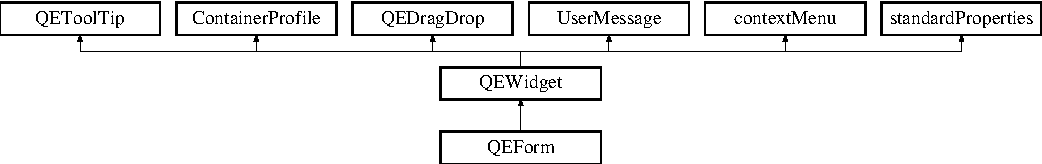
\includegraphics[height=2.204725cm]{classQEForm}
\end{center}
\end{figure}
\subsection*{Public Types}
\begin{DoxyCompactItemize}
\item 
enum {\bfseries creationOptions} \{ {\bfseries CREATION\_\-OPTION\_\-OPEN}, 
{\bfseries CREATION\_\-OPTION\_\-NEW\_\-TAB}, 
{\bfseries CREATION\_\-OPTION\_\-NEW\_\-WINDOW}
 \}
\item 
enum {\bfseries MessageFilterOptions} \{ {\bfseries Match} =  UserMessage::MESSAGE\_\-FILTER\_\-MATCH, 
{\bfseries None} =  UserMessage::MESSAGE\_\-FILTER\_\-NONE
 \}
\end{DoxyCompactItemize}
\subsection*{Public Slots}
\begin{DoxyCompactItemize}
\item 
\hypertarget{classQEForm_a2836ba4b39a104daa5fa860e59017695}{
bool {\bfseries readUiFile} ()}
\label{classQEForm_a2836ba4b39a104daa5fa860e59017695}

\item 
\hypertarget{classQEForm_abf486b58f80836901734d3ac1928b844}{
void {\bfseries launchGui} (QString guiName, QEForm::creationOptions createOption)}
\label{classQEForm_abf486b58f80836901734d3ac1928b844}

\end{DoxyCompactItemize}
\subsection*{Public Member Functions}
\begin{DoxyCompactItemize}
\item 
\hypertarget{classQEForm_a0e6f14b44a0c0e6a078f2a18f80357ad}{
{\bfseries QEForm} (QWidget $\ast$parent=0)}
\label{classQEForm_a0e6f14b44a0c0e6a078f2a18f80357ad}

\item 
\hypertarget{classQEForm_a0354e7c1f7e0e65356672d672dbc0e7a}{
{\bfseries QEForm} (const QString \&uifileNameIn, QWidget $\ast$parent=0)}
\label{classQEForm_a0354e7c1f7e0e65356672d672dbc0e7a}

\item 
\hypertarget{classQEForm_a53b4905399cc6216d25ccccf1d1e601a}{
void {\bfseries commonInit} (const bool alertIfUINoFoundIn)}
\label{classQEForm_a53b4905399cc6216d25ccccf1d1e601a}

\item 
\hypertarget{classQEForm_a6d37ea8ea852cbc0f38fdc3963dcb5ac}{
QString {\bfseries getQEGuiTitle} ()}
\label{classQEForm_a6d37ea8ea852cbc0f38fdc3963dcb5ac}

\item 
\hypertarget{classQEForm_a33ff3ace545c79ac40b935b03f4ffdc2}{
QString {\bfseries getFullFileName} ()}
\label{classQEForm_a33ff3ace545c79ac40b935b03f4ffdc2}

\item 
void \hyperlink{classQEForm_a2c6278bcd9006668e46165459015dfc5}{setVariableNameAndSubstitutions} (QString variableNameIn, QString variableNameSubstitutionsIn, unsigned int variableIndex)
\item 
\hypertarget{classQEForm_ae3152e9575274af7769470e5d5aeed4e}{
void {\bfseries setUiFileName} (QString uiFile)}
\label{classQEForm_ae3152e9575274af7769470e5d5aeed4e}

\item 
\hypertarget{classQEForm_aaccca0f00629ad77474096933b299a34}{
QString {\bfseries getUiFileName} ()}
\label{classQEForm_aaccca0f00629ad77474096933b299a34}

\item 
\hypertarget{classQEForm_ae564fdbeb6cf6f603f6f014bf85a3ad9}{
void {\bfseries setHandleGuiLaunchRequests} (bool handleGuiLaunchRequests)}
\label{classQEForm_ae564fdbeb6cf6f603f6f014bf85a3ad9}

\item 
\hypertarget{classQEForm_a8dcc30a21f0b92949c9ef330d5be33a9}{
bool {\bfseries getHandleGuiLaunchRequests} ()}
\label{classQEForm_a8dcc30a21f0b92949c9ef330d5be33a9}

\item 
\hypertarget{classQEForm_ad701a3428cf7492199bc67adc43599c6}{
void {\bfseries setResizeContents} (bool resizeContentsIn)}
\label{classQEForm_ad701a3428cf7492199bc67adc43599c6}

\item 
\hypertarget{classQEForm_a4f07864f8376f3b5be1865aff1324a54}{
bool {\bfseries getResizeContents} ()}
\label{classQEForm_a4f07864f8376f3b5be1865aff1324a54}

\item 
\hypertarget{classQEForm_a5a0fe62cf54d7107b5575195b6f94f41}{
QString {\bfseries getContainedFrameworkVersion} ()}
\label{classQEForm_a5a0fe62cf54d7107b5575195b6f94f41}

\item 
\hypertarget{classQEForm_a144be07abd87acd1edd238befbd667b8}{
QString {\bfseries getUniqueIdentifier} ()}
\label{classQEForm_a144be07abd87acd1edd238befbd667b8}

\item 
\hypertarget{classQEForm_a84666268c3af6024eaf1d443e761b606}{
void {\bfseries setUniqueIdentifier} (QString name)}
\label{classQEForm_a84666268c3af6024eaf1d443e761b606}

\item 
\hypertarget{classQEForm_ae6c3e00324dd52803bee95f4ca335280}{
void {\bfseries setVariableNameSubstitutionsProperty} (QString variableNameSubstitutions)}
\label{classQEForm_ae6c3e00324dd52803bee95f4ca335280}

\item 
\hypertarget{classQEForm_a17e348ecd1fca01767adbfabc1c3915b}{
QString {\bfseries getVariableNameSubstitutionsProperty} ()}
\label{classQEForm_a17e348ecd1fca01767adbfabc1c3915b}

\item 
\hypertarget{classQEForm_a7381a1191c48e620e9c7e99d23380d9b}{
MessageFilterOptions {\bfseries getMessageFormFilter} ()}
\label{classQEForm_a7381a1191c48e620e9c7e99d23380d9b}

\item 
\hypertarget{classQEForm_a7dc4ee4eed388213f1f334e1bcfa9128}{
void {\bfseries setMessageFormFilter} (MessageFilterOptions messageFormFilter)}
\label{classQEForm_a7dc4ee4eed388213f1f334e1bcfa9128}

\item 
\hypertarget{classQEForm_a9cd263542053a4205356b8c150adfb3d}{
MessageFilterOptions {\bfseries getMessageSourceFilter} ()}
\label{classQEForm_a9cd263542053a4205356b8c150adfb3d}

\item 
\hypertarget{classQEForm_a760522f9b3caa4464ae5bd5943170503}{
void {\bfseries setMessageSourceFilter} (MessageFilterOptions messageSourceFilter)}
\label{classQEForm_a760522f9b3caa4464ae5bd5943170503}

\end{DoxyCompactItemize}
\subsection*{Protected Member Functions}
\begin{DoxyCompactItemize}
\item 
\hypertarget{classQEForm_a7723570d747554fd0e9052221bacc490}{
void {\bfseries setVariableNameSubstitutions} (QString variableNameSubstitutionsIn)}
\label{classQEForm_a7723570d747554fd0e9052221bacc490}

\end{DoxyCompactItemize}
\subsection*{Protected Attributes}
\begin{DoxyCompactItemize}
\item 
\hypertarget{classQEForm_a5f3f5d19eb0ba253ddf59850d0af9ce2}{
QString {\bfseries uiFileName}}
\label{classQEForm_a5f3f5d19eb0ba253ddf59850d0af9ce2}

\item 
\hypertarget{classQEForm_a807b1f79c591190b9ec4f3b7faaa1b41}{
QString {\bfseries fullUiFileName}}
\label{classQEForm_a807b1f79c591190b9ec4f3b7faaa1b41}

\item 
\hypertarget{classQEForm_a7f0f5bbd7355432b8c8b935ce4848ac7}{
bool {\bfseries handleGuiLaunchRequests}}
\label{classQEForm_a7f0f5bbd7355432b8c8b935ce4848ac7}

\item 
\hypertarget{classQEForm_a5bf449b3a82cca85e8c5d8ecaf9d8358}{
bool {\bfseries resizeContents}}
\label{classQEForm_a5bf449b3a82cca85e8c5d8ecaf9d8358}

\end{DoxyCompactItemize}
\subsection*{Properties}
\begin{DoxyCompactItemize}
\item 
\hypertarget{classQEForm_a723c32581e3f8fa33dfd8ab2bc19d98d}{
QString {\bfseries uiFile}}
\label{classQEForm_a723c32581e3f8fa33dfd8ab2bc19d98d}

\item 
\hypertarget{classQEForm_a11e694dda9889b6944df8d7b5d88f3c2}{
QString {\bfseries variableSubstitutions}}
\label{classQEForm_a11e694dda9889b6944df8d7b5d88f3c2}

\item 
\hypertarget{classQEForm_a41f501bf76da6cea688f76fe5add3f32}{
unsigned {\bfseries int}}
\label{classQEForm_a41f501bf76da6cea688f76fe5add3f32}

\item 
\hypertarget{classQEForm_afc5f05f2edc783103206792a900ca07a}{
MessageFilterOptions {\bfseries messageFormFilter}}
\label{classQEForm_afc5f05f2edc783103206792a900ca07a}

\item 
\hypertarget{classQEForm_a7b6b0b67ac1019b3c0d9746cf1ed2135}{
MessageFilterOptions {\bfseries messageSourceFilter}}
\label{classQEForm_a7b6b0b67ac1019b3c0d9746cf1ed2135}

\end{DoxyCompactItemize}


\subsection{Member Function Documentation}
\hypertarget{classQEForm_a2c6278bcd9006668e46165459015dfc5}{
\index{QEForm@{QEForm}!setVariableNameAndSubstitutions@{setVariableNameAndSubstitutions}}
\index{setVariableNameAndSubstitutions@{setVariableNameAndSubstitutions}!QEForm@{QEForm}}
\subsubsection[{setVariableNameAndSubstitutions}]{\setlength{\rightskip}{0pt plus 5cm}void QEForm::setVariableNameAndSubstitutions (
\begin{DoxyParamCaption}
\item[{QString}]{variableNameIn, }
\item[{QString}]{variableNameSubstitutionsIn, }
\item[{unsigned int}]{variableIndex}
\end{DoxyParamCaption}
)\hspace{0.3cm}{\ttfamily  \mbox{[}virtual\mbox{]}}}}
\label{classQEForm_a2c6278bcd9006668e46165459015dfc5}
Virtual function that may be implimented by users of \hyperlink{classQEWidget}{QEWidget} to update variable names and macro substitutions. A default is provided that is suitible in most cases. 

Reimplemented from \hyperlink{classQEWidget_aad46c00865cd37a2221ea69fbaee8806}{QEWidget}.



The documentation for this class was generated from the following files:\begin{DoxyCompactItemize}
\item 
/tmp/epicsqt/trunk/framework/widgets/QEForm/QEForm.h\item 
/tmp/epicsqt/trunk/framework/widgets/QEForm/QEForm.cpp\end{DoxyCompactItemize}

\hypertarget{classQEFrame}{
\section{QEFrame Class Reference}
\label{classQEFrame}\index{QEFrame@{QEFrame}}
}
Inheritance diagram for QEFrame:\begin{figure}[H]
\begin{center}
\leavevmode
\includegraphics[height=2.204725cm]{classQEFrame}
\end{center}
\end{figure}
\subsection*{Public Types}
\begin{DoxyCompactItemize}
\item 
enum \hyperlink{classQEFrame_a7f512f888a2a6f46631a382597090503}{UserLevels} \{ \hyperlink{classQEFrame_a7f512f888a2a6f46631a382597090503ae8ace5cdce21b461961fe91d9e866e08}{User} =  userLevelTypes::USERLEVEL\_\-USER, 
\hyperlink{classQEFrame_a7f512f888a2a6f46631a382597090503a9c26f1c5e07f37944ee8995df369486f}{Scientist} =  userLevelTypes::USERLEVEL\_\-SCIENTIST, 
\hyperlink{classQEFrame_a7f512f888a2a6f46631a382597090503ac51282f02e7904d94e142f51c92e3a33}{Engineer} =  userLevelTypes::USERLEVEL\_\-ENGINEER
 \}
\end{DoxyCompactItemize}
\subsection*{Public Slots}
\begin{DoxyCompactItemize}
\item 
void \hyperlink{classQEFrame_a13bfd1a9f001b309575897750d992988}{requestEnabled} (const bool \&state)
\end{DoxyCompactItemize}
\subsection*{Public Member Functions}
\begin{DoxyCompactItemize}
\item 
\hypertarget{classQEFrame_ad03ce87ab1f09f591e7c495fcdf34285}{
bool \hyperlink{classQEFrame_ad03ce87ab1f09f591e7c495fcdf34285}{isEnabled} () const }
\label{classQEFrame_ad03ce87ab1f09f591e7c495fcdf34285}

\begin{DoxyCompactList}\small\item\em Access function for \hyperlink{classQEFrame_ad2c8724a8455c554dd24fc833e8f5ff7}{enabled} property -\/ refer to \hyperlink{classQEFrame_ad2c8724a8455c554dd24fc833e8f5ff7}{enabled} property for details. \end{DoxyCompactList}\item 
\hypertarget{classQEFrame_ae7ce03cae49a4fa536690f4fdd709f7c}{
void \hyperlink{classQEFrame_ae7ce03cae49a4fa536690f4fdd709f7c}{setEnabled} (bool state)}
\label{classQEFrame_ae7ce03cae49a4fa536690f4fdd709f7c}

\begin{DoxyCompactList}\small\item\em Access function for \hyperlink{classQEFrame_ad2c8724a8455c554dd24fc833e8f5ff7}{enabled} property -\/ refer to \hyperlink{classQEFrame_ad2c8724a8455c554dd24fc833e8f5ff7}{enabled} property for details. \end{DoxyCompactList}\item 
\hypertarget{classQEFrame_ac1079d8e9e2eca3389f2ef1376aa7f0a}{
\hyperlink{classQEFrame_a7f512f888a2a6f46631a382597090503}{UserLevels} \hyperlink{classQEFrame_ac1079d8e9e2eca3389f2ef1376aa7f0a}{getUserLevelVisibilityProperty} ()}
\label{classQEFrame_ac1079d8e9e2eca3389f2ef1376aa7f0a}

\begin{DoxyCompactList}\small\item\em Access function for \hyperlink{classQEFrame_af6b93bbb318228dd8debf550d8e35bd0}{userLevelVisibility} property -\/ refer to \hyperlink{classQEFrame_af6b93bbb318228dd8debf550d8e35bd0}{userLevelVisibility} property for details. \end{DoxyCompactList}\item 
\hypertarget{classQEFrame_ac2517be8df1210e1b257e4e400abc1a5}{
void \hyperlink{classQEFrame_ac2517be8df1210e1b257e4e400abc1a5}{setUserLevelVisibilityProperty} (\hyperlink{classQEFrame_a7f512f888a2a6f46631a382597090503}{UserLevels} level)}
\label{classQEFrame_ac2517be8df1210e1b257e4e400abc1a5}

\begin{DoxyCompactList}\small\item\em Access function for \hyperlink{classQEFrame_af6b93bbb318228dd8debf550d8e35bd0}{userLevelVisibility} property -\/ refer to \hyperlink{classQEFrame_af6b93bbb318228dd8debf550d8e35bd0}{userLevelVisibility} property for details. \end{DoxyCompactList}\item 
\hypertarget{classQEFrame_a4c03b42682a7cdbeb181c2d0da071ab3}{
\hyperlink{classQEFrame_a7f512f888a2a6f46631a382597090503}{UserLevels} \hyperlink{classQEFrame_a4c03b42682a7cdbeb181c2d0da071ab3}{getUserLevelEnabledProperty} ()}
\label{classQEFrame_a4c03b42682a7cdbeb181c2d0da071ab3}

\begin{DoxyCompactList}\small\item\em Access function for \hyperlink{classQEFrame_af3d7163c6158e457d081c5de695bd064}{userLevelEnabled} property -\/ refer to \hyperlink{classQEFrame_af3d7163c6158e457d081c5de695bd064}{userLevelEnabled} property for details. \end{DoxyCompactList}\item 
\hypertarget{classQEFrame_a281a6dcc9f817f5c335df4de18f14ebb}{
void \hyperlink{classQEFrame_a281a6dcc9f817f5c335df4de18f14ebb}{setUserLevelEnabledProperty} (\hyperlink{classQEFrame_a7f512f888a2a6f46631a382597090503}{UserLevels} level)}
\label{classQEFrame_a281a6dcc9f817f5c335df4de18f14ebb}

\begin{DoxyCompactList}\small\item\em Access function for \hyperlink{classQEFrame_af3d7163c6158e457d081c5de695bd064}{userLevelEnabled} property -\/ refer to \hyperlink{classQEFrame_af3d7163c6158e457d081c5de695bd064}{userLevelEnabled} property for details. \end{DoxyCompactList}\item 
\hypertarget{classQEFrame_a220dcfa856b9da9133f445e2ae8dc1ed}{
{\bfseries QEFrame} (QWidget $\ast$parent=0)}
\label{classQEFrame_a220dcfa856b9da9133f445e2ae8dc1ed}

\item 
\hypertarget{classQEFrame_a8ecbbeada87e5438cc4647482acd4ca9}{
QSize {\bfseries sizeHint} () const }
\label{classQEFrame_a8ecbbeada87e5438cc4647482acd4ca9}

\end{DoxyCompactItemize}
\subsection*{Properties}
\begin{DoxyCompactItemize}
\item 
bool \hyperlink{classQEFrame_a1cb1946dc64c08ab7eb87c8214630a7c}{variableAsToolTip}
\item 
bool \hyperlink{classQEFrame_ad2c8724a8455c554dd24fc833e8f5ff7}{enabled}
\item 
bool \hyperlink{classQEFrame_aa50e5751ece0e089a124bc2c16270e7a}{allowDrop}
\item 
bool \hyperlink{classQEFrame_a42b6f201a511f9a3b87e2474c16c0f5b}{visible}
\item 
unsigned \hyperlink{classQEFrame_a3fdb2e6df61c380f5dbae9c0d4fe2c97}{int}
\item 
QString \hyperlink{classQEFrame_a71f5eed86516183bed1d51189e954bdc}{userLevelUserStyle}
\item 
QString \hyperlink{classQEFrame_a9de22693918199d7eb8ee743ecae1110}{userLevelScientistStyle}
\item 
QString \hyperlink{classQEFrame_ade723579d535f116cf0611d001c7bfb3}{userLevelEngineerStyle}
\item 
\hyperlink{classQEFrame_a7f512f888a2a6f46631a382597090503}{UserLevels} \hyperlink{classQEFrame_af6b93bbb318228dd8debf550d8e35bd0}{userLevelVisibility}
\item 
\hyperlink{classQEFrame_a7f512f888a2a6f46631a382597090503}{UserLevels} \hyperlink{classQEFrame_af3d7163c6158e457d081c5de695bd064}{userLevelEnabled}
\item 
bool \hyperlink{classQEFrame_ab5c6eeebcdacc6101b7082c3ff89d84b}{displayAlarmState}
\end{DoxyCompactItemize}


\subsection{Member Enumeration Documentation}
\hypertarget{classQEFrame_a7f512f888a2a6f46631a382597090503}{
\index{QEFrame@{QEFrame}!UserLevels@{UserLevels}}
\index{UserLevels@{UserLevels}!QEFrame@{QEFrame}}
\subsubsection[{UserLevels}]{\setlength{\rightskip}{0pt plus 5cm}enum {\bf QEFrame::UserLevels}}}
\label{classQEFrame_a7f512f888a2a6f46631a382597090503}
User friendly enumerations for \hyperlink{classQEFrame_af6b93bbb318228dd8debf550d8e35bd0}{userLevelVisibility} and \hyperlink{classQEFrame_af3d7163c6158e457d081c5de695bd064}{userLevelEnabled} properties -\/ refer to \hyperlink{classQEFrame_af6b93bbb318228dd8debf550d8e35bd0}{userLevelVisibility} and \hyperlink{classQEFrame_af3d7163c6158e457d081c5de695bd064}{userLevelEnabled} properties and userLevel enumeration for details. \begin{Desc}
\item[Enumerator: ]\par
\begin{description}
\index{User@{User}!QEFrame@{QEFrame}}\index{QEFrame@{QEFrame}!User@{User}}\item[{\em 
\hypertarget{classQEFrame_a7f512f888a2a6f46631a382597090503ae8ace5cdce21b461961fe91d9e866e08}{
User}
\label{classQEFrame_a7f512f888a2a6f46631a382597090503ae8ace5cdce21b461961fe91d9e866e08}
}]Refer to USERLEVEL\_\-USER for details. \index{Scientist@{Scientist}!QEFrame@{QEFrame}}\index{QEFrame@{QEFrame}!Scientist@{Scientist}}\item[{\em 
\hypertarget{classQEFrame_a7f512f888a2a6f46631a382597090503a9c26f1c5e07f37944ee8995df369486f}{
Scientist}
\label{classQEFrame_a7f512f888a2a6f46631a382597090503a9c26f1c5e07f37944ee8995df369486f}
}]Refer to USERLEVEL\_\-SCIENTIST for details. \index{Engineer@{Engineer}!QEFrame@{QEFrame}}\index{QEFrame@{QEFrame}!Engineer@{Engineer}}\item[{\em 
\hypertarget{classQEFrame_a7f512f888a2a6f46631a382597090503ac51282f02e7904d94e142f51c92e3a33}{
Engineer}
\label{classQEFrame_a7f512f888a2a6f46631a382597090503ac51282f02e7904d94e142f51c92e3a33}
}]Refer to USERLEVEL\_\-ENGINEER for details. \end{description}
\end{Desc}



\subsection{Member Function Documentation}
\hypertarget{classQEFrame_a13bfd1a9f001b309575897750d992988}{
\index{QEFrame@{QEFrame}!requestEnabled@{requestEnabled}}
\index{requestEnabled@{requestEnabled}!QEFrame@{QEFrame}}
\subsubsection[{requestEnabled}]{\setlength{\rightskip}{0pt plus 5cm}void QEFrame::requestEnabled (
\begin{DoxyParamCaption}
\item[{const bool \&}]{state}
\end{DoxyParamCaption}
)\hspace{0.3cm}{\ttfamily  \mbox{[}inline, slot\mbox{]}}}}
\label{classQEFrame_a13bfd1a9f001b309575897750d992988}
Similar to standard setEnabled slot, but allows QE widget to determine if the widget remains disabled due to invalid data. If disabled due to invalid data, a request to enable the widget will be honoured when the data is no longer invalid. 

\subsection{Property Documentation}
\hypertarget{classQEFrame_aa50e5751ece0e089a124bc2c16270e7a}{
\index{QEFrame@{QEFrame}!allowDrop@{allowDrop}}
\index{allowDrop@{allowDrop}!QEFrame@{QEFrame}}
\subsubsection[{allowDrop}]{\setlength{\rightskip}{0pt plus 5cm}bool QEFrame::allowDrop\hspace{0.3cm}{\ttfamily  \mbox{[}read, write\mbox{]}}}}
\label{classQEFrame_aa50e5751ece0e089a124bc2c16270e7a}
Allow drag/drops operations to this widget. Default is false. Any dropped text will be used as a new variable name. 

Reimplemented from \hyperlink{classQEDragDrop}{QEDragDrop}.

\hypertarget{classQEFrame_ab5c6eeebcdacc6101b7082c3ff89d84b}{
\index{QEFrame@{QEFrame}!displayAlarmState@{displayAlarmState}}
\index{displayAlarmState@{displayAlarmState}!QEFrame@{QEFrame}}
\subsubsection[{displayAlarmState}]{\setlength{\rightskip}{0pt plus 5cm}bool QEFrame::displayAlarmState\hspace{0.3cm}{\ttfamily  \mbox{[}read, write\mbox{]}}}}
\label{classQEFrame_ab5c6eeebcdacc6101b7082c3ff89d84b}
If set (default) widget will indicate the alarm state of any variable data is displaying. Typically the background colour is set to indicate the alarm state. Note, this property is included in the set of standard properties as it applies to most widgets. It will do nothing for widgets that don't display data. 

Reimplemented from \hyperlink{classstandardProperties}{standardProperties}.

\hypertarget{classQEFrame_ad2c8724a8455c554dd24fc833e8f5ff7}{
\index{QEFrame@{QEFrame}!enabled@{enabled}}
\index{enabled@{enabled}!QEFrame@{QEFrame}}
\subsubsection[{enabled}]{\setlength{\rightskip}{0pt plus 5cm}bool QEFrame::enabled\hspace{0.3cm}{\ttfamily  \mbox{[}read, write\mbox{]}}}}
\label{classQEFrame_ad2c8724a8455c554dd24fc833e8f5ff7}
Set the prefered 'enabled' state. Default is true. This property is copied to the standard Qt 'enabled' property if the data being displayed is valid. If the data being displayed is invalid the standard Qt 'enabled' property will always be set to false to indicate invalid data. The value of this property will only be copied to the standard Qt 'enabled' property once data is valid. \hypertarget{classQEFrame_a3fdb2e6df61c380f5dbae9c0d4fe2c97}{
\index{QEFrame@{QEFrame}!int@{int}}
\index{int@{int}!QEFrame@{QEFrame}}
\subsubsection[{int}]{\setlength{\rightskip}{0pt plus 5cm}unsigned QEFrame::int\hspace{0.3cm}{\ttfamily  \mbox{[}read, write\mbox{]}}}}
\label{classQEFrame_a3fdb2e6df61c380f5dbae9c0d4fe2c97}
Set the ID used by the message filtering system. Default is zero. Widgets or applications that use messages from the framework have the option of filtering on this ID. For example, by using a unique message source ID a \hyperlink{classQELog}{QELog} widget may be set up to only log messages from a select set of widgets. \hypertarget{classQEFrame_af3d7163c6158e457d081c5de695bd064}{
\index{QEFrame@{QEFrame}!userLevelEnabled@{userLevelEnabled}}
\index{userLevelEnabled@{userLevelEnabled}!QEFrame@{QEFrame}}
\subsubsection[{userLevelEnabled}]{\setlength{\rightskip}{0pt plus 5cm}{\bf UserLevels} QEFrame::userLevelEnabled\hspace{0.3cm}{\ttfamily  \mbox{[}read, write\mbox{]}}}}
\label{classQEFrame_af3d7163c6158e457d081c5de695bd064}
Lowest user level at which the widget is enabled. Default is 'User'. Used when designing GUIs that allow access to more and more detail according to the user mode. The user mode is set application wide through the \hyperlink{classQELogin}{QELogin} widget, or programatically through setUserLevel() Widgets that are always accessable should be visible at 'User'. Widgets that are only accessable to scientists managing the facility should be visible at 'Scientist'. Widgets that are only accessable to engineers maintaining the facility should be visible at 'Engineer'. \hypertarget{classQEFrame_ade723579d535f116cf0611d001c7bfb3}{
\index{QEFrame@{QEFrame}!userLevelEngineerStyle@{userLevelEngineerStyle}}
\index{userLevelEngineerStyle@{userLevelEngineerStyle}!QEFrame@{QEFrame}}
\subsubsection[{userLevelEngineerStyle}]{\setlength{\rightskip}{0pt plus 5cm}QString QEFrame::userLevelEngineerStyle\hspace{0.3cm}{\ttfamily  \mbox{[}read, write\mbox{]}}}}
\label{classQEFrame_ade723579d535f116cf0611d001c7bfb3}
Style Sheet string to be applied when the widget is displayed in 'Engineer' mode. Default is an empty string. The syntax is the standard Qt Style Sheet syntax. For example, 'background-\/color: red' This Style Sheet string will be applied by the styleManager class. Refer to the styleManager class for details about how this Style Sheet string will be merged with any pre-\/existing Style Sheet string and any Style Sheet strings generated during the display of data. \hypertarget{classQEFrame_a9de22693918199d7eb8ee743ecae1110}{
\index{QEFrame@{QEFrame}!userLevelScientistStyle@{userLevelScientistStyle}}
\index{userLevelScientistStyle@{userLevelScientistStyle}!QEFrame@{QEFrame}}
\subsubsection[{userLevelScientistStyle}]{\setlength{\rightskip}{0pt plus 5cm}QString QEFrame::userLevelScientistStyle\hspace{0.3cm}{\ttfamily  \mbox{[}read, write\mbox{]}}}}
\label{classQEFrame_a9de22693918199d7eb8ee743ecae1110}
Style Sheet string to be applied when the widget is displayed in 'Scientist' mode. Default is an empty string. The syntax is the standard Qt Style Sheet syntax. For example, 'background-\/color: red' This Style Sheet string will be applied by the styleManager class. Refer to the styleManager class for details about how this Style Sheet string will be merged with any pre-\/existing Style Sheet string and any Style Sheet strings generated during the display of data. \hypertarget{classQEFrame_a71f5eed86516183bed1d51189e954bdc}{
\index{QEFrame@{QEFrame}!userLevelUserStyle@{userLevelUserStyle}}
\index{userLevelUserStyle@{userLevelUserStyle}!QEFrame@{QEFrame}}
\subsubsection[{userLevelUserStyle}]{\setlength{\rightskip}{0pt plus 5cm}QString QEFrame::userLevelUserStyle\hspace{0.3cm}{\ttfamily  \mbox{[}read, write\mbox{]}}}}
\label{classQEFrame_a71f5eed86516183bed1d51189e954bdc}
Style Sheet string to be applied when the widget is displayed in 'User' mode. Default is an empty string. The syntax is the standard Qt Style Sheet syntax. For example, 'background-\/color: red' This Style Sheet string will be applied by the styleManager class. Refer to the styleManager class for details about how this Style Sheet string will be merged with any pre-\/existing Style Sheet string and any Style Sheet strings generated during the display of data. \hypertarget{classQEFrame_af6b93bbb318228dd8debf550d8e35bd0}{
\index{QEFrame@{QEFrame}!userLevelVisibility@{userLevelVisibility}}
\index{userLevelVisibility@{userLevelVisibility}!QEFrame@{QEFrame}}
\subsubsection[{userLevelVisibility}]{\setlength{\rightskip}{0pt plus 5cm}{\bf UserLevels} QEFrame::userLevelVisibility\hspace{0.3cm}{\ttfamily  \mbox{[}read, write\mbox{]}}}}
\label{classQEFrame_af6b93bbb318228dd8debf550d8e35bd0}
Lowest user level at which the widget is visible. Default is 'User'. Used when designing GUIs that display more and more detail according to the user mode. The user mode is set application wide through the \hyperlink{classQELogin}{QELogin} widget, or programatically through setUserLevel() Widgets that are always visible should be visible at 'User'. Widgets that are only used by scientists managing the facility should be visible at 'Scientist'. Widgets that are only used by engineers maintaining the facility should be visible at 'Engineer'. \hypertarget{classQEFrame_a1cb1946dc64c08ab7eb87c8214630a7c}{
\index{QEFrame@{QEFrame}!variableAsToolTip@{variableAsToolTip}}
\index{variableAsToolTip@{variableAsToolTip}!QEFrame@{QEFrame}}
\subsubsection[{variableAsToolTip}]{\setlength{\rightskip}{0pt plus 5cm}bool QEFrame::variableAsToolTip\hspace{0.3cm}{\ttfamily  \mbox{[}read, write\mbox{]}}}}
\label{classQEFrame_a1cb1946dc64c08ab7eb87c8214630a7c}
Use the variable as the tool tip. Default is true. Tool tip property will be overwritten by the variable name. 

Reimplemented from \hyperlink{classQEToolTip}{QEToolTip}.

\hypertarget{classQEFrame_a42b6f201a511f9a3b87e2474c16c0f5b}{
\index{QEFrame@{QEFrame}!visible@{visible}}
\index{visible@{visible}!QEFrame@{QEFrame}}
\subsubsection[{visible}]{\setlength{\rightskip}{0pt plus 5cm}bool QEFrame::visible\hspace{0.3cm}{\ttfamily  \mbox{[}read, write\mbox{]}}}}
\label{classQEFrame_a42b6f201a511f9a3b87e2474c16c0f5b}
Display the widget. Default is true. Setting this property false is usefull if widget is only used to provide a signal -\/ for example, when supplying data to a \hyperlink{classQELink}{QELink} widget. Note, when false the widget will still be visible in Qt Designer. 

The documentation for this class was generated from the following files:\begin{DoxyCompactItemize}
\item 
/tmp/epicsqt/trunk/framework/widgets/QEFrame/QEFrame.h\item 
/tmp/epicsqt/trunk/framework/widgets/QEFrame/QEFrame.cpp\end{DoxyCompactItemize}

\hypertarget{classQEGenericButton}{
\section{QEGenericButton Class Reference}
\label{classQEGenericButton}\index{QEGenericButton@{QEGenericButton}}
}
Inheritance diagram for QEGenericButton:\begin{figure}[H]
\begin{center}
\leavevmode
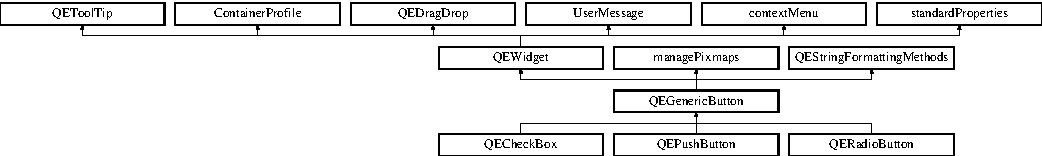
\includegraphics[height=2.097378cm]{classQEGenericButton}
\end{center}
\end{figure}
\subsection*{Public Types}
\begin{DoxyCompactItemize}
\item 
enum {\bfseries updateOptions} \{ {\bfseries UPDATE\_\-TEXT}, 
{\bfseries UPDATE\_\-ICON}, 
{\bfseries UPDATE\_\-TEXT\_\-AND\_\-ICON}, 
{\bfseries UPDATE\_\-STATE}
 \}
\end{DoxyCompactItemize}
\subsection*{Public Member Functions}
\begin{DoxyCompactItemize}
\item 
\hypertarget{classQEGenericButton_ad2c5cbe3ac38864e0816df7cac891056}{
{\bfseries QEGenericButton} (QWidget $\ast$owner)}
\label{classQEGenericButton_ad2c5cbe3ac38864e0816df7cac891056}

\item 
\hypertarget{classQEGenericButton_aeeffd2d96f84dd6a568b310aa9e60b1c}{
void {\bfseries setSubscribe} (bool subscribe)}
\label{classQEGenericButton_aeeffd2d96f84dd6a568b310aa9e60b1c}

\item 
\hypertarget{classQEGenericButton_aebe8a323388b1619475554365258b5c4}{
bool {\bfseries getSubscribe} ()}
\label{classQEGenericButton_aebe8a323388b1619475554365258b5c4}

\item 
\hypertarget{classQEGenericButton_af99ed76082a5ae2644c62d5b16942440}{
void {\bfseries setUpdateOption} (updateOptions updateOptionIn)}
\label{classQEGenericButton_af99ed76082a5ae2644c62d5b16942440}

\item 
\hypertarget{classQEGenericButton_afca2595c619728943587ffa65a1c7c6b}{
updateOptions {\bfseries getUpdateOption} ()}
\label{classQEGenericButton_afca2595c619728943587ffa65a1c7c6b}

\item 
\hypertarget{classQEGenericButton_a8754e68c2fff530abdb82fdfc6cc8aa9}{
void {\bfseries setTextAlignment} (Qt::Alignment alignment)}
\label{classQEGenericButton_a8754e68c2fff530abdb82fdfc6cc8aa9}

\item 
\hypertarget{classQEGenericButton_a6ae4c5da2ca529cb21cbe0844b57dda1}{
Qt::Alignment {\bfseries getTextAlignment} ()}
\label{classQEGenericButton_a6ae4c5da2ca529cb21cbe0844b57dda1}

\item 
\hypertarget{classQEGenericButton_a1471cc9ac63ac34544ce4ee3840b6719}{
void {\bfseries setPassword} (QString password)}
\label{classQEGenericButton_a1471cc9ac63ac34544ce4ee3840b6719}

\item 
\hypertarget{classQEGenericButton_a4080feab759638a9b83d43182ebc7f58}{
QString {\bfseries getPassword} ()}
\label{classQEGenericButton_a4080feab759638a9b83d43182ebc7f58}

\item 
\hypertarget{classQEGenericButton_aec43f479686a791c5df8113cf849c7c7}{
void {\bfseries setConfirmAction} (bool confirmRequiredIn)}
\label{classQEGenericButton_aec43f479686a791c5df8113cf849c7c7}

\item 
\hypertarget{classQEGenericButton_ac1984be89b14830bee2228061a806510}{
bool {\bfseries getConfirmAction} ()}
\label{classQEGenericButton_ac1984be89b14830bee2228061a806510}

\item 
\hypertarget{classQEGenericButton_aa267a683f2f11a4e2470ed9a49235b4f}{
void {\bfseries setWriteOnPress} (bool writeOnPress)}
\label{classQEGenericButton_aa267a683f2f11a4e2470ed9a49235b4f}

\item 
\hypertarget{classQEGenericButton_afc06622288d5438905d7b1a43860c44b}{
bool {\bfseries getWriteOnPress} ()}
\label{classQEGenericButton_afc06622288d5438905d7b1a43860c44b}

\item 
\hypertarget{classQEGenericButton_a5af8a1705a759363397655991a0b6da9}{
void {\bfseries setWriteOnRelease} (bool writeOnRelease)}
\label{classQEGenericButton_a5af8a1705a759363397655991a0b6da9}

\item 
\hypertarget{classQEGenericButton_adaf829c6a326616cead45eee7bc50000}{
bool {\bfseries getWriteOnRelease} ()}
\label{classQEGenericButton_adaf829c6a326616cead45eee7bc50000}

\item 
\hypertarget{classQEGenericButton_a989de611f13b103372f465e3d58a18b7}{
void {\bfseries setWriteOnClick} (bool writeOnClick)}
\label{classQEGenericButton_a989de611f13b103372f465e3d58a18b7}

\item 
\hypertarget{classQEGenericButton_a592b8ccdb562a1cb9a8258d72ed2ce7c}{
bool {\bfseries getWriteOnClick} ()}
\label{classQEGenericButton_a592b8ccdb562a1cb9a8258d72ed2ce7c}

\item 
\hypertarget{classQEGenericButton_a1d6f3a5c804f4889ab45dd13d5780c50}{
void {\bfseries setPressText} (QString pressText)}
\label{classQEGenericButton_a1d6f3a5c804f4889ab45dd13d5780c50}

\item 
\hypertarget{classQEGenericButton_ac2131d96a8384bd16f25a7f4aebb9022}{
QString {\bfseries getPressText} ()}
\label{classQEGenericButton_ac2131d96a8384bd16f25a7f4aebb9022}

\item 
\hypertarget{classQEGenericButton_a64a200354d9204778b75afdfb0e85f84}{
void {\bfseries setReleaseText} (QString releaseTextIn)}
\label{classQEGenericButton_a64a200354d9204778b75afdfb0e85f84}

\item 
\hypertarget{classQEGenericButton_a6322b1cb4ab8b8e7b0b404aeffbc669f}{
QString {\bfseries getReleaseText} ()}
\label{classQEGenericButton_a6322b1cb4ab8b8e7b0b404aeffbc669f}

\item 
\hypertarget{classQEGenericButton_a35ed4c2409d7af10d3d0ae9dd0ab9ae9}{
void {\bfseries setClickText} (QString clickTextIn)}
\label{classQEGenericButton_a35ed4c2409d7af10d3d0ae9dd0ab9ae9}

\item 
\hypertarget{classQEGenericButton_adc9c5638248c2ec7759a8feb5295e7c4}{
QString {\bfseries getClickText} ()}
\label{classQEGenericButton_adc9c5638248c2ec7759a8feb5295e7c4}

\item 
\hypertarget{classQEGenericButton_affa8b16866dce13bd1726ef093155611}{
void {\bfseries setClickCheckedText} (QString clickCheckedTextIn)}
\label{classQEGenericButton_affa8b16866dce13bd1726ef093155611}

\item 
\hypertarget{classQEGenericButton_a6560ee24d0327dc30d01a6d5a7bd01fb}{
QString {\bfseries getClickCheckedText} ()}
\label{classQEGenericButton_a6560ee24d0327dc30d01a6d5a7bd01fb}

\item 
\hypertarget{classQEGenericButton_a276bcc01c487455167e8e05242b4d306}{
void {\bfseries setProgram} (QString program)}
\label{classQEGenericButton_a276bcc01c487455167e8e05242b4d306}

\item 
\hypertarget{classQEGenericButton_a3296f8deab9ca68a5092815e35b1d52d}{
QString {\bfseries getProgram} ()}
\label{classQEGenericButton_a3296f8deab9ca68a5092815e35b1d52d}

\item 
\hypertarget{classQEGenericButton_a0d92db106dde516d6828fb58c9dd37e8}{
void {\bfseries setArguments} (QStringList arguments)}
\label{classQEGenericButton_a0d92db106dde516d6828fb58c9dd37e8}

\item 
\hypertarget{classQEGenericButton_af8bac549a10c0dd8ee9b9d90b4030c18}{
QStringList {\bfseries getArguments} ()}
\label{classQEGenericButton_af8bac549a10c0dd8ee9b9d90b4030c18}

\item 
\hypertarget{classQEGenericButton_a5d5e32f2ab10703aa31cd321e90c39f0}{
void {\bfseries setGuiName} (QString guiName)}
\label{classQEGenericButton_a5d5e32f2ab10703aa31cd321e90c39f0}

\item 
\hypertarget{classQEGenericButton_a403f79f9e7159277263e48b73f7cca7a}{
QString {\bfseries getGuiName} ()}
\label{classQEGenericButton_a403f79f9e7159277263e48b73f7cca7a}

\item 
\hypertarget{classQEGenericButton_a30e30457e63dc866da487258064e02c1}{
void {\bfseries setPrioritySubstitutions} (QString prioritySubstitutionsIn)}
\label{classQEGenericButton_a30e30457e63dc866da487258064e02c1}

\item 
\hypertarget{classQEGenericButton_adac082d484c513232c82274947e8b623}{
QString {\bfseries getPrioritySubstitutions} ()}
\label{classQEGenericButton_adac082d484c513232c82274947e8b623}

\item 
\hypertarget{classQEGenericButton_a3640442dd5a6f07b3cac78a16d92079c}{
void {\bfseries setCreationOption} (QEForm::creationOptions creationOption)}
\label{classQEGenericButton_a3640442dd5a6f07b3cac78a16d92079c}

\item 
\hypertarget{classQEGenericButton_a374933dfd5d97ce5d8c2e7c6509bdb8c}{
QEForm::creationOptions {\bfseries getCreationOption} ()}
\label{classQEGenericButton_a374933dfd5d97ce5d8c2e7c6509bdb8c}

\item 
\hypertarget{classQEGenericButton_ad78bb7a4c7dce75bb021c4e6eaaedf67}{
void {\bfseries setLabelTextProperty} (QString labelTextIn)}
\label{classQEGenericButton_ad78bb7a4c7dce75bb021c4e6eaaedf67}

\item 
\hypertarget{classQEGenericButton_a11f1483f1397d6547d1ed1824e42f46a}{
QString {\bfseries getLabelTextProperty} ()}
\label{classQEGenericButton_a11f1483f1397d6547d1ed1824e42f46a}

\end{DoxyCompactItemize}
\subsection*{Protected Member Functions}
\begin{DoxyCompactItemize}
\item 
\hypertarget{classQEGenericButton_a099d7ea25cb5b113bc28dba6a597f3eb}{
void {\bfseries connectionChanged} (\hyperlink{classQCaConnectionInfo}{QCaConnectionInfo} \&connectionInfo)}
\label{classQEGenericButton_a099d7ea25cb5b113bc28dba6a597f3eb}

\item 
\hypertarget{classQEGenericButton_a32fbf44e1c7a4cbf94851d511e69549f}{
void {\bfseries setGenericButtonText} (const QString \&text, \hyperlink{classQCaAlarmInfo}{QCaAlarmInfo} \&alarmInfo, \hyperlink{classQCaDateTime}{QCaDateTime} \&, const unsigned int \&variableIndex)}
\label{classQEGenericButton_a32fbf44e1c7a4cbf94851d511e69549f}

\item 
\hypertarget{classQEGenericButton_a8c47d9e60710a04e089560a4204358e4}{
void {\bfseries userPressed} ()}
\label{classQEGenericButton_a8c47d9e60710a04e089560a4204358e4}

\item 
\hypertarget{classQEGenericButton_ade9aee71af98bc722b3203759190af34}{
void {\bfseries userReleased} ()}
\label{classQEGenericButton_ade9aee71af98bc722b3203759190af34}

\item 
\hypertarget{classQEGenericButton_aa5e7d2135b2b2dd3de1649d88a170f4c}{
void {\bfseries userClicked} (bool checked)}
\label{classQEGenericButton_aa5e7d2135b2b2dd3de1649d88a170f4c}

\item 
\hypertarget{classQEGenericButton_a4d2e4da742fbf8e1bf4fcf8ee17969ee}{
void {\bfseries launchGui} (QString guiName, QEForm::creationOptions creationOption)}
\label{classQEGenericButton_a4d2e4da742fbf8e1bf4fcf8ee17969ee}

\item 
\hypertarget{classQEGenericButton_ab185c3376360c8335282e97d071490b3}{
virtual updateOptions {\bfseries getDefaultUpdateOption} ()=0}
\label{classQEGenericButton_ab185c3376360c8335282e97d071490b3}

\item 
\hypertarget{classQEGenericButton_a1265293fe6fe00c0d35f0c692d32e548}{
void {\bfseries setup} ()}
\label{classQEGenericButton_a1265293fe6fe00c0d35f0c692d32e548}

\item 
\hypertarget{classQEGenericButton_a968735c14e189b839b50704f1b28bc14}{
void {\bfseries establishConnection} (unsigned int variableIndex)}
\label{classQEGenericButton_a968735c14e189b839b50704f1b28bc14}

\end{DoxyCompactItemize}


The documentation for this class was generated from the following files:\begin{DoxyCompactItemize}
\item 
/tmp/epicsqt/trunk/framework/widgets/QEButton/QEGenericButton.h\item 
/tmp/epicsqt/trunk/framework/widgets/QEButton/QEGenericButton.cpp\end{DoxyCompactItemize}

\hypertarget{classQEGenericEdit}{
\section{QEGenericEdit Class Reference}
\label{classQEGenericEdit}\index{QEGenericEdit@{QEGenericEdit}}
}
Inheritance diagram for QEGenericEdit:\begin{figure}[H]
\begin{center}
\leavevmode
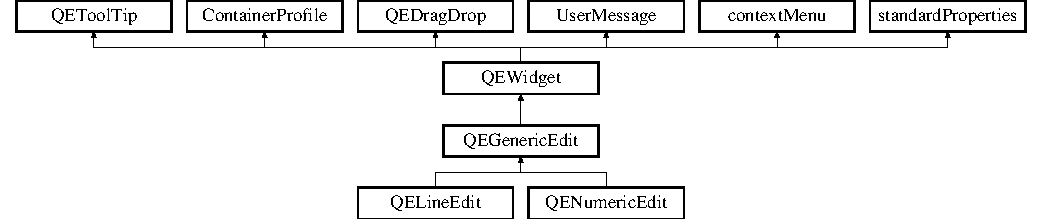
\includegraphics[height=2.939633cm]{classQEGenericEdit}
\end{center}
\end{figure}
\subsection*{Public Types}
\begin{DoxyCompactItemize}
\item 
enum \hyperlink{classQEGenericEdit_a0d4ee4dc910113b53e1396e0736f28b7}{UserLevels} \{ \hyperlink{classQEGenericEdit_a0d4ee4dc910113b53e1396e0736f28b7a58230231609299c2f6c1cab4a7d5aedb}{User} =  userLevelTypes::USERLEVEL\_\-USER, 
\hyperlink{classQEGenericEdit_a0d4ee4dc910113b53e1396e0736f28b7ac942f3d3484a3a5bd465dcd2b3f52f19}{Scientist} =  userLevelTypes::USERLEVEL\_\-SCIENTIST, 
\hyperlink{classQEGenericEdit_a0d4ee4dc910113b53e1396e0736f28b7a17b7bf8f749cca831e3c8f05a4a519fa}{Engineer} =  userLevelTypes::USERLEVEL\_\-ENGINEER
 \}
\end{DoxyCompactItemize}
\subsection*{Public Slots}
\begin{DoxyCompactItemize}
\item 
void \hyperlink{classQEGenericEdit_a698af066af7eb1d5e5ad1bdc74c02536}{requestEnabled} (const bool \&state)
\end{DoxyCompactItemize}
\subsection*{Signals}
\begin{DoxyCompactItemize}
\item 
\hypertarget{classQEGenericEdit_ae82720428e2102045d6cce86c4b902f4}{
void \hyperlink{classQEGenericEdit_ae82720428e2102045d6cce86c4b902f4}{userChange} (const QVariant \&oldValue, const QVariant \&newValue, const QVariant \&lastValue)}
\label{classQEGenericEdit_ae82720428e2102045d6cce86c4b902f4}

\begin{DoxyCompactList}\small\item\em Internal use only. Used by \hyperlink{classQEConfiguredLayout}{QEConfiguredLayout} to be notified when one of its widgets has written something. \end{DoxyCompactList}\item 
\hypertarget{classQEGenericEdit_ab3039c4d18b0b2c55ca1698f5c91c04c}{
void \hyperlink{classQEGenericEdit_ab3039c4d18b0b2c55ca1698f5c91c04c}{requestResend} ()}
\label{classQEGenericEdit_ab3039c4d18b0b2c55ca1698f5c91c04c}

\begin{DoxyCompactList}\small\item\em Internal use only. Used when changing a property value to force a re-\/display to reflect the new property value. \end{DoxyCompactList}\end{DoxyCompactItemize}
\subsection*{Public Member Functions}
\begin{DoxyCompactItemize}
\item 
\hypertarget{classQEGenericEdit_af447107cc2d856bac1ddba568f9f6fd3}{
bool \hyperlink{classQEGenericEdit_af447107cc2d856bac1ddba568f9f6fd3}{isEnabled} () const }
\label{classQEGenericEdit_af447107cc2d856bac1ddba568f9f6fd3}

\begin{DoxyCompactList}\small\item\em Access function for \hyperlink{classQEGenericEdit_a7f543d99ef8b0b0ab2550b9e9f6cbbce}{enabled} property -\/ refer to \hyperlink{classQEGenericEdit_a7f543d99ef8b0b0ab2550b9e9f6cbbce}{enabled} property for details. \end{DoxyCompactList}\item 
\hypertarget{classQEGenericEdit_ac6f6a91a6554b3afdbb800f3409a6fe0}{
void \hyperlink{classQEGenericEdit_ac6f6a91a6554b3afdbb800f3409a6fe0}{setEnabled} (bool state)}
\label{classQEGenericEdit_ac6f6a91a6554b3afdbb800f3409a6fe0}

\begin{DoxyCompactList}\small\item\em Access function for \hyperlink{classQEGenericEdit_a7f543d99ef8b0b0ab2550b9e9f6cbbce}{enabled} property -\/ refer to \hyperlink{classQEGenericEdit_a7f543d99ef8b0b0ab2550b9e9f6cbbce}{enabled} property for details. \end{DoxyCompactList}\item 
\hypertarget{classQEGenericEdit_abb214e5915ef497ebc7f3ddce212ec74}{
\hyperlink{classQEGenericEdit_a0d4ee4dc910113b53e1396e0736f28b7}{UserLevels} \hyperlink{classQEGenericEdit_abb214e5915ef497ebc7f3ddce212ec74}{getUserLevelVisibilityProperty} ()}
\label{classQEGenericEdit_abb214e5915ef497ebc7f3ddce212ec74}

\begin{DoxyCompactList}\small\item\em Access function for \hyperlink{classQEGenericEdit_a7f0733266f39549d361cdf65e34ebd30}{userLevelVisibility} property -\/ refer to \hyperlink{classQEGenericEdit_a7f0733266f39549d361cdf65e34ebd30}{userLevelVisibility} property for details. \end{DoxyCompactList}\item 
\hypertarget{classQEGenericEdit_aacd858afb29729dfbf0f27e6178c4d46}{
void \hyperlink{classQEGenericEdit_aacd858afb29729dfbf0f27e6178c4d46}{setUserLevelVisibilityProperty} (\hyperlink{classQEGenericEdit_a0d4ee4dc910113b53e1396e0736f28b7}{UserLevels} level)}
\label{classQEGenericEdit_aacd858afb29729dfbf0f27e6178c4d46}

\begin{DoxyCompactList}\small\item\em Access function for \hyperlink{classQEGenericEdit_a7f0733266f39549d361cdf65e34ebd30}{userLevelVisibility} property -\/ refer to \hyperlink{classQEGenericEdit_a7f0733266f39549d361cdf65e34ebd30}{userLevelVisibility} property for details. \end{DoxyCompactList}\item 
\hypertarget{classQEGenericEdit_a68003d4b2c5ff1c6bea247a63a3de9fd}{
\hyperlink{classQEGenericEdit_a0d4ee4dc910113b53e1396e0736f28b7}{UserLevels} \hyperlink{classQEGenericEdit_a68003d4b2c5ff1c6bea247a63a3de9fd}{getUserLevelEnabledProperty} ()}
\label{classQEGenericEdit_a68003d4b2c5ff1c6bea247a63a3de9fd}

\begin{DoxyCompactList}\small\item\em Access function for \hyperlink{classQEGenericEdit_ae18520d83fec62603db7e658efe00e3c}{userLevelEnabled} property -\/ refer to \hyperlink{classQEGenericEdit_ae18520d83fec62603db7e658efe00e3c}{userLevelEnabled} property for details. \end{DoxyCompactList}\item 
\hypertarget{classQEGenericEdit_a5b2ed96d60d2e12262a4e27a62036e11}{
void \hyperlink{classQEGenericEdit_a5b2ed96d60d2e12262a4e27a62036e11}{setUserLevelEnabledProperty} (\hyperlink{classQEGenericEdit_a0d4ee4dc910113b53e1396e0736f28b7}{UserLevels} level)}
\label{classQEGenericEdit_a5b2ed96d60d2e12262a4e27a62036e11}

\begin{DoxyCompactList}\small\item\em Access function for \hyperlink{classQEGenericEdit_ae18520d83fec62603db7e658efe00e3c}{userLevelEnabled} property -\/ refer to \hyperlink{classQEGenericEdit_ae18520d83fec62603db7e658efe00e3c}{userLevelEnabled} property for details. \end{DoxyCompactList}\item 
\hyperlink{classQEGenericEdit_aad24935d20ac13d05d79a7dac3619a2a}{QEGenericEdit} (QWidget $\ast$parent=0)
\item 
\hyperlink{classQEGenericEdit_a3a4960d3dd72d32329a6c02a5be2113c}{QEGenericEdit} (const QString \&variableName, QWidget $\ast$parent=0)
\item 
void \hyperlink{classQEGenericEdit_a49653dc548a0bfa35d8a34caabd21859}{setWriteOnLoseFocus} (bool writeOnLoseFocus)
\item 
bool \hyperlink{classQEGenericEdit_ae3e8108427c11e7199856793ed4197f1}{getWriteOnLoseFocus} ()
\item 
void \hyperlink{classQEGenericEdit_a1ac64f86c547d8196f6b6a9aad336ffd}{setWriteOnEnter} (bool writeOnEnter)
\item 
bool \hyperlink{classQEGenericEdit_a7e0ab81eb7b0826635cf546d9f25abef}{getWriteOnEnter} ()
\item 
void \hyperlink{classQEGenericEdit_aff9f621c2d7ec4e33e4b1ce5a99d0cf4}{setWriteOnFinish} (bool writeOnFinish)
\item 
bool \hyperlink{classQEGenericEdit_a8f9c3b15e14008c69c83fbb9e0cb1e71}{getWriteOnFinish} ()
\item 
void \hyperlink{classQEGenericEdit_a6925d54620cd6b7298b83a5867c23254}{setConfirmWrite} (bool confirmWrite)
\item 
bool \hyperlink{classQEGenericEdit_ae7da757a225d1b76ffee8e7d39ce4c79}{getConfirmWrite} ()
\item 
void \hyperlink{classQEGenericEdit_a3743dc52396cff2b7a1599a2845d682e}{setSubscribe} (bool subscribe)
\item 
bool \hyperlink{classQEGenericEdit_a4402bb99875a061dab8870b5d66eff1d}{getSubscribe} ()
\item 
\hypertarget{classQEGenericEdit_a5ce70de489d5618a3e5dc8d6bb6fc9f3}{
void {\bfseries writeValue} (\hyperlink{classqcaobject_1_1QCaObject}{qcaobject::QCaObject} $\ast$qca, QVariant newValue)}
\label{classQEGenericEdit_a5ce70de489d5618a3e5dc8d6bb6fc9f3}

\end{DoxyCompactItemize}
\subsection*{Protected Member Functions}
\begin{DoxyCompactItemize}
\item 
\hypertarget{classQEGenericEdit_ad02189df7183d90a526c3f3d5ac0b6ae}{
void {\bfseries setDataIfNoFocus} (const QVariant \&value, \hyperlink{classQCaAlarmInfo}{QCaAlarmInfo} \&alarmInfo, \hyperlink{classQCaDateTime}{QCaDateTime} \&dateTime)}
\label{classQEGenericEdit_ad02189df7183d90a526c3f3d5ac0b6ae}

\item 
\hypertarget{classQEGenericEdit_a6fa0a363dd4854ea0eb798fd25cd1b73}{
bool {\bfseries getIsConnected} ()}
\label{classQEGenericEdit_a6fa0a363dd4854ea0eb798fd25cd1b73}

\item 
\hypertarget{classQEGenericEdit_ab34598025968f64b8f7076d2d863b569}{
bool {\bfseries testAndClearIsFirstUpdate} ()}
\label{classQEGenericEdit_ab34598025968f64b8f7076d2d863b569}

\item 
\hypertarget{classQEGenericEdit_ad48cf45ad365708c88d421aab99c5c4d}{
virtual void {\bfseries setValue} (const QVariant \&value)=0}
\label{classQEGenericEdit_ad48cf45ad365708c88d421aab99c5c4d}

\item 
\hypertarget{classQEGenericEdit_ae31c252612988eec9a3161b759c1beaf}{
virtual QVariant {\bfseries getValue} ()=0}
\label{classQEGenericEdit_ae31c252612988eec9a3161b759c1beaf}

\item 
\hypertarget{classQEGenericEdit_a38e8a142c71a0527aeea7d44f9cf59c2}{
virtual bool {\bfseries writeData} (const QVariant \&value, QString \&message)=0}
\label{classQEGenericEdit_a38e8a142c71a0527aeea7d44f9cf59c2}

\item 
\hypertarget{classQEGenericEdit_a22c63f981233ad42124d10eef6b7af3b}{
void \hyperlink{classQEGenericEdit_a22c63f981233ad42124d10eef6b7af3b}{writeNow} ()}
\label{classQEGenericEdit_a22c63f981233ad42124d10eef6b7af3b}

\begin{DoxyCompactList}\small\item\em Write the value now. \end{DoxyCompactList}\end{DoxyCompactItemize}
\subsection*{Protected Attributes}
\begin{DoxyCompactItemize}
\item 
\hypertarget{classQEGenericEdit_a8d40a5e0f2ef98ea5ca57acbd0ed68b1}{
QVariant {\bfseries lastValue}}
\label{classQEGenericEdit_a8d40a5e0f2ef98ea5ca57acbd0ed68b1}

\item 
\hypertarget{classQEGenericEdit_a65637bd64f8990a6f41c010201626f08}{
QVariant {\bfseries lastUserValue}}
\label{classQEGenericEdit_a65637bd64f8990a6f41c010201626f08}

\item 
\hypertarget{classQEGenericEdit_a5c5676a2a611fcbb8626450d584fcbd7}{
bool {\bfseries messageDialogPresent}}
\label{classQEGenericEdit_a5c5676a2a611fcbb8626450d584fcbd7}

\item 
\hypertarget{classQEGenericEdit_a290d7c70baea6277dbcd86d4e8ab4f9d}{
bool {\bfseries writeFailMessageDialogPresent}}
\label{classQEGenericEdit_a290d7c70baea6277dbcd86d4e8ab4f9d}

\item 
\hypertarget{classQEGenericEdit_a4ed3d543eec420b2f5e1bb6af9f86bf6}{
bool {\bfseries isConnected}}
\label{classQEGenericEdit_a4ed3d543eec420b2f5e1bb6af9f86bf6}

\end{DoxyCompactItemize}
\subsection*{Properties}
\begin{DoxyCompactItemize}
\item 
QString \hyperlink{classQEGenericEdit_a4d5d7d260857021e0714ec47e0bba9f7}{variable}
\item 
QString \hyperlink{classQEGenericEdit_a4cbf09c0d505553217dc9880d0987382}{variableSubstitutions}
\item 
bool \hyperlink{classQEGenericEdit_a3cb8e9d1d34565e89d1c484504975fb5}{subscribe}
\item 
bool \hyperlink{classQEGenericEdit_a2da40951e678a9e31413b87b45d59c64}{writeOnLoseFocus}
\item 
bool \hyperlink{classQEGenericEdit_a4555b5e4928e65bde2f522e26078fa84}{writeOnEnter}
\item 
bool \hyperlink{classQEGenericEdit_a72daabd68fba3750b5633a9ec610e5d3}{writeOnFinish}
\item 
bool \hyperlink{classQEGenericEdit_ab04f43d93b0c5d813cd5f85c5069d4bd}{confirmWrite}
\item 
bool \hyperlink{classQEGenericEdit_a9173bf85137b00076d02c7d1f88323f9}{variableAsToolTip}
\item 
bool \hyperlink{classQEGenericEdit_a7f543d99ef8b0b0ab2550b9e9f6cbbce}{enabled}
\item 
bool \hyperlink{classQEGenericEdit_ad9a855d077672a0728845f478445b1b0}{allowDrop}
\item 
bool \hyperlink{classQEGenericEdit_af3d5533b501f2d763431cb1b5b2aa7e0}{visible}
\item 
unsigned \hyperlink{classQEGenericEdit_a9e520be7f9bbbede4efc7fb4c9cebd9d}{int}
\item 
QString \hyperlink{classQEGenericEdit_a13421ac7b96c448d3ed92d69713b52d5}{userLevelUserStyle}
\item 
QString \hyperlink{classQEGenericEdit_a98fef02145d98961debe3cdc8fa8cb9c}{userLevelScientistStyle}
\item 
QString \hyperlink{classQEGenericEdit_ab4d7c33ffbce0d809dc4fc078e99f924}{userLevelEngineerStyle}
\item 
\hyperlink{classQEGenericEdit_a0d4ee4dc910113b53e1396e0736f28b7}{UserLevels} \hyperlink{classQEGenericEdit_a7f0733266f39549d361cdf65e34ebd30}{userLevelVisibility}
\item 
\hyperlink{classQEGenericEdit_a0d4ee4dc910113b53e1396e0736f28b7}{UserLevels} \hyperlink{classQEGenericEdit_ae18520d83fec62603db7e658efe00e3c}{userLevelEnabled}
\item 
bool \hyperlink{classQEGenericEdit_a663da3081feabe1b0d0194a4e1e744f8}{displayAlarmState}
\end{DoxyCompactItemize}


\subsection{Member Enumeration Documentation}
\hypertarget{classQEGenericEdit_a0d4ee4dc910113b53e1396e0736f28b7}{
\index{QEGenericEdit@{QEGenericEdit}!UserLevels@{UserLevels}}
\index{UserLevels@{UserLevels}!QEGenericEdit@{QEGenericEdit}}
\subsubsection[{UserLevels}]{\setlength{\rightskip}{0pt plus 5cm}enum {\bf QEGenericEdit::UserLevels}}}
\label{classQEGenericEdit_a0d4ee4dc910113b53e1396e0736f28b7}
User friendly enumerations for \hyperlink{classQEGenericEdit_a7f0733266f39549d361cdf65e34ebd30}{userLevelVisibility} and \hyperlink{classQEGenericEdit_ae18520d83fec62603db7e658efe00e3c}{userLevelEnabled} properties -\/ refer to \hyperlink{classQEGenericEdit_a7f0733266f39549d361cdf65e34ebd30}{userLevelVisibility} and \hyperlink{classQEGenericEdit_ae18520d83fec62603db7e658efe00e3c}{userLevelEnabled} properties and userLevel enumeration for details. \begin{Desc}
\item[Enumerator: ]\par
\begin{description}
\index{User@{User}!QEGenericEdit@{QEGenericEdit}}\index{QEGenericEdit@{QEGenericEdit}!User@{User}}\item[{\em 
\hypertarget{classQEGenericEdit_a0d4ee4dc910113b53e1396e0736f28b7a58230231609299c2f6c1cab4a7d5aedb}{
User}
\label{classQEGenericEdit_a0d4ee4dc910113b53e1396e0736f28b7a58230231609299c2f6c1cab4a7d5aedb}
}]Refer to USERLEVEL\_\-USER for details. \index{Scientist@{Scientist}!QEGenericEdit@{QEGenericEdit}}\index{QEGenericEdit@{QEGenericEdit}!Scientist@{Scientist}}\item[{\em 
\hypertarget{classQEGenericEdit_a0d4ee4dc910113b53e1396e0736f28b7ac942f3d3484a3a5bd465dcd2b3f52f19}{
Scientist}
\label{classQEGenericEdit_a0d4ee4dc910113b53e1396e0736f28b7ac942f3d3484a3a5bd465dcd2b3f52f19}
}]Refer to USERLEVEL\_\-SCIENTIST for details. \index{Engineer@{Engineer}!QEGenericEdit@{QEGenericEdit}}\index{QEGenericEdit@{QEGenericEdit}!Engineer@{Engineer}}\item[{\em 
\hypertarget{classQEGenericEdit_a0d4ee4dc910113b53e1396e0736f28b7a17b7bf8f749cca831e3c8f05a4a519fa}{
Engineer}
\label{classQEGenericEdit_a0d4ee4dc910113b53e1396e0736f28b7a17b7bf8f749cca831e3c8f05a4a519fa}
}]Refer to USERLEVEL\_\-ENGINEER for details. \end{description}
\end{Desc}



\subsection{Constructor \& Destructor Documentation}
\hypertarget{classQEGenericEdit_aad24935d20ac13d05d79a7dac3619a2a}{
\index{QEGenericEdit@{QEGenericEdit}!QEGenericEdit@{QEGenericEdit}}
\index{QEGenericEdit@{QEGenericEdit}!QEGenericEdit@{QEGenericEdit}}
\subsubsection[{QEGenericEdit}]{\setlength{\rightskip}{0pt plus 5cm}QEGenericEdit::QEGenericEdit (
\begin{DoxyParamCaption}
\item[{QWidget $\ast$}]{parent = {\ttfamily 0}}
\end{DoxyParamCaption}
)}}
\label{classQEGenericEdit_aad24935d20ac13d05d79a7dac3619a2a}
Create without a variable. Use setVariableNameProperty() and setSubstitutionsProperty() to define a variable and, optionally, macro substitutions later. \hypertarget{classQEGenericEdit_a3a4960d3dd72d32329a6c02a5be2113c}{
\index{QEGenericEdit@{QEGenericEdit}!QEGenericEdit@{QEGenericEdit}}
\index{QEGenericEdit@{QEGenericEdit}!QEGenericEdit@{QEGenericEdit}}
\subsubsection[{QEGenericEdit}]{\setlength{\rightskip}{0pt plus 5cm}QEGenericEdit::QEGenericEdit (
\begin{DoxyParamCaption}
\item[{const QString \&}]{variableName, }
\item[{QWidget $\ast$}]{parent = {\ttfamily 0}}
\end{DoxyParamCaption}
)}}
\label{classQEGenericEdit_a3a4960d3dd72d32329a6c02a5be2113c}
Create with a variable. A connection is automatically established. If macro substitutions are required, create without a variable and set the variable and macro substitutions after creation. 

\subsection{Member Function Documentation}
\hypertarget{classQEGenericEdit_ae7da757a225d1b76ffee8e7d39ce4c79}{
\index{QEGenericEdit@{QEGenericEdit}!getConfirmWrite@{getConfirmWrite}}
\index{getConfirmWrite@{getConfirmWrite}!QEGenericEdit@{QEGenericEdit}}
\subsubsection[{getConfirmWrite}]{\setlength{\rightskip}{0pt plus 5cm}bool QEGenericEdit::getConfirmWrite (
\begin{DoxyParamCaption}
{}
\end{DoxyParamCaption}
)}}
\label{classQEGenericEdit_ae7da757a225d1b76ffee8e7d39ce4c79}
Returns 'true' if this widget will ask for confirmation (using a dialog box) prior to writing data. \hypertarget{classQEGenericEdit_a4402bb99875a061dab8870b5d66eff1d}{
\index{QEGenericEdit@{QEGenericEdit}!getSubscribe@{getSubscribe}}
\index{getSubscribe@{getSubscribe}!QEGenericEdit@{QEGenericEdit}}
\subsubsection[{getSubscribe}]{\setlength{\rightskip}{0pt plus 5cm}bool QEGenericEdit::getSubscribe (
\begin{DoxyParamCaption}
{}
\end{DoxyParamCaption}
)}}
\label{classQEGenericEdit_a4402bb99875a061dab8870b5d66eff1d}
Returns 'true' if this widget subscribes for data updates and displays current data. \hypertarget{classQEGenericEdit_a7e0ab81eb7b0826635cf546d9f25abef}{
\index{QEGenericEdit@{QEGenericEdit}!getWriteOnEnter@{getWriteOnEnter}}
\index{getWriteOnEnter@{getWriteOnEnter}!QEGenericEdit@{QEGenericEdit}}
\subsubsection[{getWriteOnEnter}]{\setlength{\rightskip}{0pt plus 5cm}bool QEGenericEdit::getWriteOnEnter (
\begin{DoxyParamCaption}
{}
\end{DoxyParamCaption}
)}}
\label{classQEGenericEdit_a7e0ab81eb7b0826635cf546d9f25abef}
Returns 'true' if this widget writes any changes when the user presses 'enter'. \hypertarget{classQEGenericEdit_a8f9c3b15e14008c69c83fbb9e0cb1e71}{
\index{QEGenericEdit@{QEGenericEdit}!getWriteOnFinish@{getWriteOnFinish}}
\index{getWriteOnFinish@{getWriteOnFinish}!QEGenericEdit@{QEGenericEdit}}
\subsubsection[{getWriteOnFinish}]{\setlength{\rightskip}{0pt plus 5cm}bool QEGenericEdit::getWriteOnFinish (
\begin{DoxyParamCaption}
{}
\end{DoxyParamCaption}
)}}
\label{classQEGenericEdit_a8f9c3b15e14008c69c83fbb9e0cb1e71}
Returns 'true' if this widget writes any changes when the user finished editing (the QLineEdit 'editingFinished' signal is emitted). \hypertarget{classQEGenericEdit_ae3e8108427c11e7199856793ed4197f1}{
\index{QEGenericEdit@{QEGenericEdit}!getWriteOnLoseFocus@{getWriteOnLoseFocus}}
\index{getWriteOnLoseFocus@{getWriteOnLoseFocus}!QEGenericEdit@{QEGenericEdit}}
\subsubsection[{getWriteOnLoseFocus}]{\setlength{\rightskip}{0pt plus 5cm}bool QEGenericEdit::getWriteOnLoseFocus (
\begin{DoxyParamCaption}
{}
\end{DoxyParamCaption}
)}}
\label{classQEGenericEdit_ae3e8108427c11e7199856793ed4197f1}
Returns 'true' if this widget automatically writes any changes when it loses focus. \hypertarget{classQEGenericEdit_a698af066af7eb1d5e5ad1bdc74c02536}{
\index{QEGenericEdit@{QEGenericEdit}!requestEnabled@{requestEnabled}}
\index{requestEnabled@{requestEnabled}!QEGenericEdit@{QEGenericEdit}}
\subsubsection[{requestEnabled}]{\setlength{\rightskip}{0pt plus 5cm}void QEGenericEdit::requestEnabled (
\begin{DoxyParamCaption}
\item[{const bool \&}]{state}
\end{DoxyParamCaption}
)\hspace{0.3cm}{\ttfamily  \mbox{[}inline, slot\mbox{]}}}}
\label{classQEGenericEdit_a698af066af7eb1d5e5ad1bdc74c02536}
Similar to standard setEnabled slot, but allows QE widget to determine if the widget remains disabled due to invalid data. If disabled due to invalid data, a request to enable the widget will be honoured when the data is no longer invalid. \hypertarget{classQEGenericEdit_a6925d54620cd6b7298b83a5867c23254}{
\index{QEGenericEdit@{QEGenericEdit}!setConfirmWrite@{setConfirmWrite}}
\index{setConfirmWrite@{setConfirmWrite}!QEGenericEdit@{QEGenericEdit}}
\subsubsection[{setConfirmWrite}]{\setlength{\rightskip}{0pt plus 5cm}void QEGenericEdit::setConfirmWrite (
\begin{DoxyParamCaption}
\item[{bool}]{confirmWrite}
\end{DoxyParamCaption}
)}}
\label{classQEGenericEdit_a6925d54620cd6b7298b83a5867c23254}
Sets if this widget will ask for confirmation (using a dialog box) prior to writing data. Default is 'false' (will not ask for confirmation (using a dialog box) prior to writing data). \hypertarget{classQEGenericEdit_a3743dc52396cff2b7a1599a2845d682e}{
\index{QEGenericEdit@{QEGenericEdit}!setSubscribe@{setSubscribe}}
\index{setSubscribe@{setSubscribe}!QEGenericEdit@{QEGenericEdit}}
\subsubsection[{setSubscribe}]{\setlength{\rightskip}{0pt plus 5cm}void QEGenericEdit::setSubscribe (
\begin{DoxyParamCaption}
\item[{bool}]{subscribe}
\end{DoxyParamCaption}
)}}
\label{classQEGenericEdit_a3743dc52396cff2b7a1599a2845d682e}
Sets if this widget subscribes for data updates and displays current data. Default is 'true' (subscribes for and displays data updates) \hypertarget{classQEGenericEdit_a1ac64f86c547d8196f6b6a9aad336ffd}{
\index{QEGenericEdit@{QEGenericEdit}!setWriteOnEnter@{setWriteOnEnter}}
\index{setWriteOnEnter@{setWriteOnEnter}!QEGenericEdit@{QEGenericEdit}}
\subsubsection[{setWriteOnEnter}]{\setlength{\rightskip}{0pt plus 5cm}void QEGenericEdit::setWriteOnEnter (
\begin{DoxyParamCaption}
\item[{bool}]{writeOnEnter}
\end{DoxyParamCaption}
)}}
\label{classQEGenericEdit_a1ac64f86c547d8196f6b6a9aad336ffd}
Sets if this widget writes any changes when the user presses 'enter'. Note, the current value will be written even if the user has not changed it. Default is 'true' (writes any changes when the user presses 'enter'). \hypertarget{classQEGenericEdit_aff9f621c2d7ec4e33e4b1ce5a99d0cf4}{
\index{QEGenericEdit@{QEGenericEdit}!setWriteOnFinish@{setWriteOnFinish}}
\index{setWriteOnFinish@{setWriteOnFinish}!QEGenericEdit@{QEGenericEdit}}
\subsubsection[{setWriteOnFinish}]{\setlength{\rightskip}{0pt plus 5cm}void QEGenericEdit::setWriteOnFinish (
\begin{DoxyParamCaption}
\item[{bool}]{writeOnFinish}
\end{DoxyParamCaption}
)}}
\label{classQEGenericEdit_aff9f621c2d7ec4e33e4b1ce5a99d0cf4}
Sets if this widget writes any changes when the user finished editing (the QLineEdit 'editingFinished' signal is emitted). No writing occurs if no changes were made. Default is 'true' (writes any changes when the QLineEdit 'editingFinished' signal is emitted). \hypertarget{classQEGenericEdit_a49653dc548a0bfa35d8a34caabd21859}{
\index{QEGenericEdit@{QEGenericEdit}!setWriteOnLoseFocus@{setWriteOnLoseFocus}}
\index{setWriteOnLoseFocus@{setWriteOnLoseFocus}!QEGenericEdit@{QEGenericEdit}}
\subsubsection[{setWriteOnLoseFocus}]{\setlength{\rightskip}{0pt plus 5cm}void QEGenericEdit::setWriteOnLoseFocus (
\begin{DoxyParamCaption}
\item[{bool}]{writeOnLoseFocus}
\end{DoxyParamCaption}
)}}
\label{classQEGenericEdit_a49653dc548a0bfa35d8a34caabd21859}
Sets if this widget automatically writes any changes when it loses focus. Default is 'false' (does not write any changes when it loses focus). 

\subsection{Property Documentation}
\hypertarget{classQEGenericEdit_ad9a855d077672a0728845f478445b1b0}{
\index{QEGenericEdit@{QEGenericEdit}!allowDrop@{allowDrop}}
\index{allowDrop@{allowDrop}!QEGenericEdit@{QEGenericEdit}}
\subsubsection[{allowDrop}]{\setlength{\rightskip}{0pt plus 5cm}bool QEGenericEdit::allowDrop\hspace{0.3cm}{\ttfamily  \mbox{[}read, write\mbox{]}}}}
\label{classQEGenericEdit_ad9a855d077672a0728845f478445b1b0}
Allow drag/drops operations to this widget. Default is false. Any dropped text will be used as a new variable name. 

Reimplemented from \hyperlink{classQEDragDrop}{QEDragDrop}.

\hypertarget{classQEGenericEdit_ab04f43d93b0c5d813cd5f85c5069d4bd}{
\index{QEGenericEdit@{QEGenericEdit}!confirmWrite@{confirmWrite}}
\index{confirmWrite@{confirmWrite}!QEGenericEdit@{QEGenericEdit}}
\subsubsection[{confirmWrite}]{\setlength{\rightskip}{0pt plus 5cm}bool QEGenericEdit::confirmWrite\hspace{0.3cm}{\ttfamily  \mbox{[}read, write\mbox{]}}}}
\label{classQEGenericEdit_ab04f43d93b0c5d813cd5f85c5069d4bd}
Sets if this widget will ask for confirmation (using a dialog box) prior to writing data. Default is 'false' (will not ask for confirmation (using a dialog box) prior to writing data). \hypertarget{classQEGenericEdit_a663da3081feabe1b0d0194a4e1e744f8}{
\index{QEGenericEdit@{QEGenericEdit}!displayAlarmState@{displayAlarmState}}
\index{displayAlarmState@{displayAlarmState}!QEGenericEdit@{QEGenericEdit}}
\subsubsection[{displayAlarmState}]{\setlength{\rightskip}{0pt plus 5cm}bool QEGenericEdit::displayAlarmState\hspace{0.3cm}{\ttfamily  \mbox{[}read, write\mbox{]}}}}
\label{classQEGenericEdit_a663da3081feabe1b0d0194a4e1e744f8}
If set (default) widget will indicate the alarm state of any variable data is displaying. Typically the background colour is set to indicate the alarm state. Note, this property is included in the set of standard properties as it applies to most widgets. It will do nothing for widgets that don't display data. 

Reimplemented from \hyperlink{classstandardProperties}{standardProperties}.

\hypertarget{classQEGenericEdit_a7f543d99ef8b0b0ab2550b9e9f6cbbce}{
\index{QEGenericEdit@{QEGenericEdit}!enabled@{enabled}}
\index{enabled@{enabled}!QEGenericEdit@{QEGenericEdit}}
\subsubsection[{enabled}]{\setlength{\rightskip}{0pt plus 5cm}bool QEGenericEdit::enabled\hspace{0.3cm}{\ttfamily  \mbox{[}read, write\mbox{]}}}}
\label{classQEGenericEdit_a7f543d99ef8b0b0ab2550b9e9f6cbbce}
Set the prefered 'enabled' state. Default is true. This property is copied to the standard Qt 'enabled' property if the data being displayed is valid. If the data being displayed is invalid the standard Qt 'enabled' property will always be set to false to indicate invalid data. The value of this property will only be copied to the standard Qt 'enabled' property once data is valid. \hypertarget{classQEGenericEdit_a9e520be7f9bbbede4efc7fb4c9cebd9d}{
\index{QEGenericEdit@{QEGenericEdit}!int@{int}}
\index{int@{int}!QEGenericEdit@{QEGenericEdit}}
\subsubsection[{int}]{\setlength{\rightskip}{0pt plus 5cm}unsigned QEGenericEdit::int\hspace{0.3cm}{\ttfamily  \mbox{[}read, write\mbox{]}}}}
\label{classQEGenericEdit_a9e520be7f9bbbede4efc7fb4c9cebd9d}
Set the ID used by the message filtering system. Default is zero. Widgets or applications that use messages from the framework have the option of filtering on this ID. For example, by using a unique message source ID a \hyperlink{classQELog}{QELog} widget may be set up to only log messages from a select set of widgets. 

Reimplemented in \hyperlink{classQELineEdit_adf8beec6661bba8c6a8a277c0dcd2bdd}{QELineEdit}.

\hypertarget{classQEGenericEdit_a3cb8e9d1d34565e89d1c484504975fb5}{
\index{QEGenericEdit@{QEGenericEdit}!subscribe@{subscribe}}
\index{subscribe@{subscribe}!QEGenericEdit@{QEGenericEdit}}
\subsubsection[{subscribe}]{\setlength{\rightskip}{0pt plus 5cm}bool QEGenericEdit::subscribe\hspace{0.3cm}{\ttfamily  \mbox{[}read, write\mbox{]}}}}
\label{classQEGenericEdit_a3cb8e9d1d34565e89d1c484504975fb5}
Sets if this widget subscribes for data updates and displays current data. Default is 'true' (subscribes for and displays data updates) 

Reimplemented from \hyperlink{classQEWidget}{QEWidget}.

\hypertarget{classQEGenericEdit_ae18520d83fec62603db7e658efe00e3c}{
\index{QEGenericEdit@{QEGenericEdit}!userLevelEnabled@{userLevelEnabled}}
\index{userLevelEnabled@{userLevelEnabled}!QEGenericEdit@{QEGenericEdit}}
\subsubsection[{userLevelEnabled}]{\setlength{\rightskip}{0pt plus 5cm}{\bf UserLevels} QEGenericEdit::userLevelEnabled\hspace{0.3cm}{\ttfamily  \mbox{[}read, write\mbox{]}}}}
\label{classQEGenericEdit_ae18520d83fec62603db7e658efe00e3c}
Lowest user level at which the widget is enabled. Default is 'User'. Used when designing GUIs that allow access to more and more detail according to the user mode. The user mode is set application wide through the \hyperlink{classQELogin}{QELogin} widget, or programatically through setUserLevel() Widgets that are always accessable should be visible at 'User'. Widgets that are only accessable to scientists managing the facility should be visible at 'Scientist'. Widgets that are only accessable to engineers maintaining the facility should be visible at 'Engineer'. \hypertarget{classQEGenericEdit_ab4d7c33ffbce0d809dc4fc078e99f924}{
\index{QEGenericEdit@{QEGenericEdit}!userLevelEngineerStyle@{userLevelEngineerStyle}}
\index{userLevelEngineerStyle@{userLevelEngineerStyle}!QEGenericEdit@{QEGenericEdit}}
\subsubsection[{userLevelEngineerStyle}]{\setlength{\rightskip}{0pt plus 5cm}QString QEGenericEdit::userLevelEngineerStyle\hspace{0.3cm}{\ttfamily  \mbox{[}read, write\mbox{]}}}}
\label{classQEGenericEdit_ab4d7c33ffbce0d809dc4fc078e99f924}
Style Sheet string to be applied when the widget is displayed in 'Engineer' mode. Default is an empty string. The syntax is the standard Qt Style Sheet syntax. For example, 'background-\/color: red' This Style Sheet string will be applied by the styleManager class. Refer to the styleManager class for details about how this Style Sheet string will be merged with any pre-\/existing Style Sheet string and any Style Sheet strings generated during the display of data. \hypertarget{classQEGenericEdit_a98fef02145d98961debe3cdc8fa8cb9c}{
\index{QEGenericEdit@{QEGenericEdit}!userLevelScientistStyle@{userLevelScientistStyle}}
\index{userLevelScientistStyle@{userLevelScientistStyle}!QEGenericEdit@{QEGenericEdit}}
\subsubsection[{userLevelScientistStyle}]{\setlength{\rightskip}{0pt plus 5cm}QString QEGenericEdit::userLevelScientistStyle\hspace{0.3cm}{\ttfamily  \mbox{[}read, write\mbox{]}}}}
\label{classQEGenericEdit_a98fef02145d98961debe3cdc8fa8cb9c}
Style Sheet string to be applied when the widget is displayed in 'Scientist' mode. Default is an empty string. The syntax is the standard Qt Style Sheet syntax. For example, 'background-\/color: red' This Style Sheet string will be applied by the styleManager class. Refer to the styleManager class for details about how this Style Sheet string will be merged with any pre-\/existing Style Sheet string and any Style Sheet strings generated during the display of data. \hypertarget{classQEGenericEdit_a13421ac7b96c448d3ed92d69713b52d5}{
\index{QEGenericEdit@{QEGenericEdit}!userLevelUserStyle@{userLevelUserStyle}}
\index{userLevelUserStyle@{userLevelUserStyle}!QEGenericEdit@{QEGenericEdit}}
\subsubsection[{userLevelUserStyle}]{\setlength{\rightskip}{0pt plus 5cm}QString QEGenericEdit::userLevelUserStyle\hspace{0.3cm}{\ttfamily  \mbox{[}read, write\mbox{]}}}}
\label{classQEGenericEdit_a13421ac7b96c448d3ed92d69713b52d5}
Style Sheet string to be applied when the widget is displayed in 'User' mode. Default is an empty string. The syntax is the standard Qt Style Sheet syntax. For example, 'background-\/color: red' This Style Sheet string will be applied by the styleManager class. Refer to the styleManager class for details about how this Style Sheet string will be merged with any pre-\/existing Style Sheet string and any Style Sheet strings generated during the display of data. \hypertarget{classQEGenericEdit_a7f0733266f39549d361cdf65e34ebd30}{
\index{QEGenericEdit@{QEGenericEdit}!userLevelVisibility@{userLevelVisibility}}
\index{userLevelVisibility@{userLevelVisibility}!QEGenericEdit@{QEGenericEdit}}
\subsubsection[{userLevelVisibility}]{\setlength{\rightskip}{0pt plus 5cm}{\bf UserLevels} QEGenericEdit::userLevelVisibility\hspace{0.3cm}{\ttfamily  \mbox{[}read, write\mbox{]}}}}
\label{classQEGenericEdit_a7f0733266f39549d361cdf65e34ebd30}
Lowest user level at which the widget is visible. Default is 'User'. Used when designing GUIs that display more and more detail according to the user mode. The user mode is set application wide through the \hyperlink{classQELogin}{QELogin} widget, or programatically through setUserLevel() Widgets that are always visible should be visible at 'User'. Widgets that are only used by scientists managing the facility should be visible at 'Scientist'. Widgets that are only used by engineers maintaining the facility should be visible at 'Engineer'. \hypertarget{classQEGenericEdit_a4d5d7d260857021e0714ec47e0bba9f7}{
\index{QEGenericEdit@{QEGenericEdit}!variable@{variable}}
\index{variable@{variable}!QEGenericEdit@{QEGenericEdit}}
\subsubsection[{variable}]{\setlength{\rightskip}{0pt plus 5cm}QString QEGenericEdit::variable\hspace{0.3cm}{\ttfamily  \mbox{[}read, write\mbox{]}}}}
\label{classQEGenericEdit_a4d5d7d260857021e0714ec47e0bba9f7}
EPICS variable name (CA PV) \hypertarget{classQEGenericEdit_a9173bf85137b00076d02c7d1f88323f9}{
\index{QEGenericEdit@{QEGenericEdit}!variableAsToolTip@{variableAsToolTip}}
\index{variableAsToolTip@{variableAsToolTip}!QEGenericEdit@{QEGenericEdit}}
\subsubsection[{variableAsToolTip}]{\setlength{\rightskip}{0pt plus 5cm}bool QEGenericEdit::variableAsToolTip\hspace{0.3cm}{\ttfamily  \mbox{[}read, write\mbox{]}}}}
\label{classQEGenericEdit_a9173bf85137b00076d02c7d1f88323f9}
Use the variable as the tool tip. Default is true. Tool tip property will be overwritten by the variable name. 

Reimplemented from \hyperlink{classQEToolTip}{QEToolTip}.

\hypertarget{classQEGenericEdit_a4cbf09c0d505553217dc9880d0987382}{
\index{QEGenericEdit@{QEGenericEdit}!variableSubstitutions@{variableSubstitutions}}
\index{variableSubstitutions@{variableSubstitutions}!QEGenericEdit@{QEGenericEdit}}
\subsubsection[{variableSubstitutions}]{\setlength{\rightskip}{0pt plus 5cm}QString QEGenericEdit::variableSubstitutions\hspace{0.3cm}{\ttfamily  \mbox{[}read, write\mbox{]}}}}
\label{classQEGenericEdit_a4cbf09c0d505553217dc9880d0987382}
Macro substitutions. The default is no substitutions. The format is NAME1=VALUE1\mbox{[},\mbox{]} NAME2=VALUE2... Values may be quoted strings. For example, 'PUMP=PMP3, NAME = \char`\"{}My Pump\char`\"{}' These substitutions are applied to variable names for all QE widgets. In some widgets are are also used for other purposes. \hypertarget{classQEGenericEdit_af3d5533b501f2d763431cb1b5b2aa7e0}{
\index{QEGenericEdit@{QEGenericEdit}!visible@{visible}}
\index{visible@{visible}!QEGenericEdit@{QEGenericEdit}}
\subsubsection[{visible}]{\setlength{\rightskip}{0pt plus 5cm}bool QEGenericEdit::visible\hspace{0.3cm}{\ttfamily  \mbox{[}read, write\mbox{]}}}}
\label{classQEGenericEdit_af3d5533b501f2d763431cb1b5b2aa7e0}
Display the widget. Default is true. Setting this property false is usefull if widget is only used to provide a signal -\/ for example, when supplying data to a \hyperlink{classQELink}{QELink} widget. Note, when false the widget will still be visible in Qt Designer. \hypertarget{classQEGenericEdit_a4555b5e4928e65bde2f522e26078fa84}{
\index{QEGenericEdit@{QEGenericEdit}!writeOnEnter@{writeOnEnter}}
\index{writeOnEnter@{writeOnEnter}!QEGenericEdit@{QEGenericEdit}}
\subsubsection[{writeOnEnter}]{\setlength{\rightskip}{0pt plus 5cm}bool QEGenericEdit::writeOnEnter\hspace{0.3cm}{\ttfamily  \mbox{[}read, write\mbox{]}}}}
\label{classQEGenericEdit_a4555b5e4928e65bde2f522e26078fa84}
Sets if this widget writes any changes when the user presses 'enter'. Note, the current value will be written even if the user has not changed it. Default is 'true' (writes any changes when the user presses 'enter'). \hypertarget{classQEGenericEdit_a72daabd68fba3750b5633a9ec610e5d3}{
\index{QEGenericEdit@{QEGenericEdit}!writeOnFinish@{writeOnFinish}}
\index{writeOnFinish@{writeOnFinish}!QEGenericEdit@{QEGenericEdit}}
\subsubsection[{writeOnFinish}]{\setlength{\rightskip}{0pt plus 5cm}bool QEGenericEdit::writeOnFinish\hspace{0.3cm}{\ttfamily  \mbox{[}read, write\mbox{]}}}}
\label{classQEGenericEdit_a72daabd68fba3750b5633a9ec610e5d3}
Sets if this widget writes any changes when the user finished editing (the QLineEdit 'editingFinished' signal is emitted). No writing occurs if no changes were made. Default is 'true' (writes any changes when the QLineEdit 'editingFinished' signal is emitted). \hypertarget{classQEGenericEdit_a2da40951e678a9e31413b87b45d59c64}{
\index{QEGenericEdit@{QEGenericEdit}!writeOnLoseFocus@{writeOnLoseFocus}}
\index{writeOnLoseFocus@{writeOnLoseFocus}!QEGenericEdit@{QEGenericEdit}}
\subsubsection[{writeOnLoseFocus}]{\setlength{\rightskip}{0pt plus 5cm}bool QEGenericEdit::writeOnLoseFocus\hspace{0.3cm}{\ttfamily  \mbox{[}read, write\mbox{]}}}}
\label{classQEGenericEdit_a2da40951e678a9e31413b87b45d59c64}
Sets if this widget automatically writes any changes when it loses focus. Default is 'false' (does not write any changes when it loses focus). 

The documentation for this class was generated from the following files:\begin{DoxyCompactItemize}
\item 
/tmp/epicsqt/trunk/framework/widgets/QELineEdit/QEGenericEdit.h\item 
/tmp/epicsqt/trunk/framework/widgets/QELineEdit/QEGenericEdit.cpp\end{DoxyCompactItemize}

\hypertarget{classQEGroupBox}{
\section{QEGroupBox Class Reference}
\label{classQEGroupBox}\index{QEGroupBox@{QEGroupBox}}
}
Inheritance diagram for QEGroupBox:\begin{figure}[H]
\begin{center}
\leavevmode
\includegraphics[height=2.204725cm]{classQEGroupBox}
\end{center}
\end{figure}
\subsection*{Public Types}
\begin{DoxyCompactItemize}
\item 
enum \hyperlink{classQEGroupBox_ad5a2c847226aa067c44f86ed42ddaba8}{UserLevels} \{ \hyperlink{classQEGroupBox_ad5a2c847226aa067c44f86ed42ddaba8af266b3d599e59d87c500c8a5e870b4f6}{User} =  userLevelTypes::USERLEVEL\_\-USER, 
\hyperlink{classQEGroupBox_ad5a2c847226aa067c44f86ed42ddaba8a37e2ed84893fe0df0649aad7e32704be}{Scientist} =  userLevelTypes::USERLEVEL\_\-SCIENTIST, 
\hyperlink{classQEGroupBox_ad5a2c847226aa067c44f86ed42ddaba8af3fa6b68de62f134049b7b1f4b7a6310}{Engineer} =  userLevelTypes::USERLEVEL\_\-ENGINEER
 \}
\end{DoxyCompactItemize}
\subsection*{Public Slots}
\begin{DoxyCompactItemize}
\item 
void \hyperlink{classQEGroupBox_a54ec85b75f96e59486c7d1fc2d6b0577}{requestEnabled} (const bool \&state)
\end{DoxyCompactItemize}
\subsection*{Public Member Functions}
\begin{DoxyCompactItemize}
\item 
\hypertarget{classQEGroupBox_a3195278553902c367ea7c6cb459e8c95}{
bool \hyperlink{classQEGroupBox_a3195278553902c367ea7c6cb459e8c95}{isEnabled} () const }
\label{classQEGroupBox_a3195278553902c367ea7c6cb459e8c95}

\begin{DoxyCompactList}\small\item\em Access function for \hyperlink{classQEGroupBox_aa1baaa6c2cec673d24addade65acd2f3}{enabled} property -\/ refer to \hyperlink{classQEGroupBox_aa1baaa6c2cec673d24addade65acd2f3}{enabled} property for details. \end{DoxyCompactList}\item 
\hypertarget{classQEGroupBox_a49dc81cd7e031acfd6264943fce36894}{
void \hyperlink{classQEGroupBox_a49dc81cd7e031acfd6264943fce36894}{setEnabled} (bool state)}
\label{classQEGroupBox_a49dc81cd7e031acfd6264943fce36894}

\begin{DoxyCompactList}\small\item\em Access function for \hyperlink{classQEGroupBox_aa1baaa6c2cec673d24addade65acd2f3}{enabled} property -\/ refer to \hyperlink{classQEGroupBox_aa1baaa6c2cec673d24addade65acd2f3}{enabled} property for details. \end{DoxyCompactList}\item 
\hypertarget{classQEGroupBox_ab4ddfd5ae4bbc1033a1e46b9a16348b6}{
\hyperlink{classQEGroupBox_ad5a2c847226aa067c44f86ed42ddaba8}{UserLevels} \hyperlink{classQEGroupBox_ab4ddfd5ae4bbc1033a1e46b9a16348b6}{getUserLevelVisibilityProperty} ()}
\label{classQEGroupBox_ab4ddfd5ae4bbc1033a1e46b9a16348b6}

\begin{DoxyCompactList}\small\item\em Access function for \hyperlink{classQEGroupBox_af592de1c93b6a919b9431c0dc3868dcc}{userLevelVisibility} property -\/ refer to \hyperlink{classQEGroupBox_af592de1c93b6a919b9431c0dc3868dcc}{userLevelVisibility} property for details. \end{DoxyCompactList}\item 
\hypertarget{classQEGroupBox_a79bea0ec99f314068a759cfee71f7b7e}{
void \hyperlink{classQEGroupBox_a79bea0ec99f314068a759cfee71f7b7e}{setUserLevelVisibilityProperty} (\hyperlink{classQEGroupBox_ad5a2c847226aa067c44f86ed42ddaba8}{UserLevels} level)}
\label{classQEGroupBox_a79bea0ec99f314068a759cfee71f7b7e}

\begin{DoxyCompactList}\small\item\em Access function for \hyperlink{classQEGroupBox_af592de1c93b6a919b9431c0dc3868dcc}{userLevelVisibility} property -\/ refer to \hyperlink{classQEGroupBox_af592de1c93b6a919b9431c0dc3868dcc}{userLevelVisibility} property for details. \end{DoxyCompactList}\item 
\hypertarget{classQEGroupBox_afb7c34703384e33cdebe0668ec2598fb}{
\hyperlink{classQEGroupBox_ad5a2c847226aa067c44f86ed42ddaba8}{UserLevels} \hyperlink{classQEGroupBox_afb7c34703384e33cdebe0668ec2598fb}{getUserLevelEnabledProperty} ()}
\label{classQEGroupBox_afb7c34703384e33cdebe0668ec2598fb}

\begin{DoxyCompactList}\small\item\em Access function for \hyperlink{classQEGroupBox_ad26f2a98dccecbdfbe200e3f032262fb}{userLevelEnabled} property -\/ refer to \hyperlink{classQEGroupBox_ad26f2a98dccecbdfbe200e3f032262fb}{userLevelEnabled} property for details. \end{DoxyCompactList}\item 
\hypertarget{classQEGroupBox_aaad9aec1cb3d889696495d0a46a9838e}{
void \hyperlink{classQEGroupBox_aaad9aec1cb3d889696495d0a46a9838e}{setUserLevelEnabledProperty} (\hyperlink{classQEGroupBox_ad5a2c847226aa067c44f86ed42ddaba8}{UserLevels} level)}
\label{classQEGroupBox_aaad9aec1cb3d889696495d0a46a9838e}

\begin{DoxyCompactList}\small\item\em Access function for \hyperlink{classQEGroupBox_ad26f2a98dccecbdfbe200e3f032262fb}{userLevelEnabled} property -\/ refer to \hyperlink{classQEGroupBox_ad26f2a98dccecbdfbe200e3f032262fb}{userLevelEnabled} property for details. \end{DoxyCompactList}\item 
\hypertarget{classQEGroupBox_ab859db65dcf651db87f9f42479cb16c5}{
{\bfseries QEGroupBox} (QWidget $\ast$parent=0)}
\label{classQEGroupBox_ab859db65dcf651db87f9f42479cb16c5}

\item 
\hypertarget{classQEGroupBox_ab4c7f8cb36d7538ab554396db1861505}{
QSize {\bfseries sizeHint} () const }
\label{classQEGroupBox_ab4c7f8cb36d7538ab554396db1861505}

\end{DoxyCompactItemize}
\subsection*{Properties}
\begin{DoxyCompactItemize}
\item 
bool \hyperlink{classQEGroupBox_a98b187722b014911112842e2bf315720}{variableAsToolTip}
\item 
bool \hyperlink{classQEGroupBox_aa1baaa6c2cec673d24addade65acd2f3}{enabled}
\item 
bool \hyperlink{classQEGroupBox_a7a41419b7a252414abd344fbdf76f6d3}{allowDrop}
\item 
bool \hyperlink{classQEGroupBox_a05617d911ff363073f9b1f2c40e2db71}{visible}
\item 
unsigned \hyperlink{classQEGroupBox_a717ad8ca5b5dc1f44b118d31a2a5736d}{int}
\item 
QString \hyperlink{classQEGroupBox_a31519ee2f188352af49695b774c0794a}{userLevelUserStyle}
\item 
QString \hyperlink{classQEGroupBox_a5d1841110a7dd0733755640f5ebd0713}{userLevelScientistStyle}
\item 
QString \hyperlink{classQEGroupBox_a56cdaa9cf2d9e1682f7f249c9b949361}{userLevelEngineerStyle}
\item 
\hyperlink{classQEGroupBox_ad5a2c847226aa067c44f86ed42ddaba8}{UserLevels} \hyperlink{classQEGroupBox_af592de1c93b6a919b9431c0dc3868dcc}{userLevelVisibility}
\item 
\hyperlink{classQEGroupBox_ad5a2c847226aa067c44f86ed42ddaba8}{UserLevels} \hyperlink{classQEGroupBox_ad26f2a98dccecbdfbe200e3f032262fb}{userLevelEnabled}
\item 
bool \hyperlink{classQEGroupBox_ad429fc7e8a9f1dfc0fd3c66f8b7801d8}{displayAlarmState}
\end{DoxyCompactItemize}


\subsection{Member Enumeration Documentation}
\hypertarget{classQEGroupBox_ad5a2c847226aa067c44f86ed42ddaba8}{
\index{QEGroupBox@{QEGroupBox}!UserLevels@{UserLevels}}
\index{UserLevels@{UserLevels}!QEGroupBox@{QEGroupBox}}
\subsubsection[{UserLevels}]{\setlength{\rightskip}{0pt plus 5cm}enum {\bf QEGroupBox::UserLevels}}}
\label{classQEGroupBox_ad5a2c847226aa067c44f86ed42ddaba8}
User friendly enumerations for \hyperlink{classQEGroupBox_af592de1c93b6a919b9431c0dc3868dcc}{userLevelVisibility} and \hyperlink{classQEGroupBox_ad26f2a98dccecbdfbe200e3f032262fb}{userLevelEnabled} properties -\/ refer to \hyperlink{classQEGroupBox_af592de1c93b6a919b9431c0dc3868dcc}{userLevelVisibility} and \hyperlink{classQEGroupBox_ad26f2a98dccecbdfbe200e3f032262fb}{userLevelEnabled} properties and userLevel enumeration for details. \begin{Desc}
\item[Enumerator: ]\par
\begin{description}
\index{User@{User}!QEGroupBox@{QEGroupBox}}\index{QEGroupBox@{QEGroupBox}!User@{User}}\item[{\em 
\hypertarget{classQEGroupBox_ad5a2c847226aa067c44f86ed42ddaba8af266b3d599e59d87c500c8a5e870b4f6}{
User}
\label{classQEGroupBox_ad5a2c847226aa067c44f86ed42ddaba8af266b3d599e59d87c500c8a5e870b4f6}
}]Refer to USERLEVEL\_\-USER for details. \index{Scientist@{Scientist}!QEGroupBox@{QEGroupBox}}\index{QEGroupBox@{QEGroupBox}!Scientist@{Scientist}}\item[{\em 
\hypertarget{classQEGroupBox_ad5a2c847226aa067c44f86ed42ddaba8a37e2ed84893fe0df0649aad7e32704be}{
Scientist}
\label{classQEGroupBox_ad5a2c847226aa067c44f86ed42ddaba8a37e2ed84893fe0df0649aad7e32704be}
}]Refer to USERLEVEL\_\-SCIENTIST for details. \index{Engineer@{Engineer}!QEGroupBox@{QEGroupBox}}\index{QEGroupBox@{QEGroupBox}!Engineer@{Engineer}}\item[{\em 
\hypertarget{classQEGroupBox_ad5a2c847226aa067c44f86ed42ddaba8af3fa6b68de62f134049b7b1f4b7a6310}{
Engineer}
\label{classQEGroupBox_ad5a2c847226aa067c44f86ed42ddaba8af3fa6b68de62f134049b7b1f4b7a6310}
}]Refer to USERLEVEL\_\-ENGINEER for details. \end{description}
\end{Desc}



\subsection{Member Function Documentation}
\hypertarget{classQEGroupBox_a54ec85b75f96e59486c7d1fc2d6b0577}{
\index{QEGroupBox@{QEGroupBox}!requestEnabled@{requestEnabled}}
\index{requestEnabled@{requestEnabled}!QEGroupBox@{QEGroupBox}}
\subsubsection[{requestEnabled}]{\setlength{\rightskip}{0pt plus 5cm}void QEGroupBox::requestEnabled (
\begin{DoxyParamCaption}
\item[{const bool \&}]{state}
\end{DoxyParamCaption}
)\hspace{0.3cm}{\ttfamily  \mbox{[}inline, slot\mbox{]}}}}
\label{classQEGroupBox_a54ec85b75f96e59486c7d1fc2d6b0577}
Similar to standard setEnabled slot, but allows QE widget to determine if the widget remains disabled due to invalid data. If disabled due to invalid data, a request to enable the widget will be honoured when the data is no longer invalid. 

\subsection{Property Documentation}
\hypertarget{classQEGroupBox_a7a41419b7a252414abd344fbdf76f6d3}{
\index{QEGroupBox@{QEGroupBox}!allowDrop@{allowDrop}}
\index{allowDrop@{allowDrop}!QEGroupBox@{QEGroupBox}}
\subsubsection[{allowDrop}]{\setlength{\rightskip}{0pt plus 5cm}bool QEGroupBox::allowDrop\hspace{0.3cm}{\ttfamily  \mbox{[}read, write\mbox{]}}}}
\label{classQEGroupBox_a7a41419b7a252414abd344fbdf76f6d3}
Allow drag/drops operations to this widget. Default is false. Any dropped text will be used as a new variable name. 

Reimplemented from \hyperlink{classQEDragDrop}{QEDragDrop}.

\hypertarget{classQEGroupBox_ad429fc7e8a9f1dfc0fd3c66f8b7801d8}{
\index{QEGroupBox@{QEGroupBox}!displayAlarmState@{displayAlarmState}}
\index{displayAlarmState@{displayAlarmState}!QEGroupBox@{QEGroupBox}}
\subsubsection[{displayAlarmState}]{\setlength{\rightskip}{0pt plus 5cm}bool QEGroupBox::displayAlarmState\hspace{0.3cm}{\ttfamily  \mbox{[}read, write\mbox{]}}}}
\label{classQEGroupBox_ad429fc7e8a9f1dfc0fd3c66f8b7801d8}
If set (default) widget will indicate the alarm state of any variable data is displaying. Typically the background colour is set to indicate the alarm state. Note, this property is included in the set of standard properties as it applies to most widgets. It will do nothing for widgets that don't display data. 

Reimplemented from \hyperlink{classstandardProperties}{standardProperties}.

\hypertarget{classQEGroupBox_aa1baaa6c2cec673d24addade65acd2f3}{
\index{QEGroupBox@{QEGroupBox}!enabled@{enabled}}
\index{enabled@{enabled}!QEGroupBox@{QEGroupBox}}
\subsubsection[{enabled}]{\setlength{\rightskip}{0pt plus 5cm}bool QEGroupBox::enabled\hspace{0.3cm}{\ttfamily  \mbox{[}read, write\mbox{]}}}}
\label{classQEGroupBox_aa1baaa6c2cec673d24addade65acd2f3}
Set the prefered 'enabled' state. Default is true. This property is copied to the standard Qt 'enabled' property if the data being displayed is valid. If the data being displayed is invalid the standard Qt 'enabled' property will always be set to false to indicate invalid data. The value of this property will only be copied to the standard Qt 'enabled' property once data is valid. \hypertarget{classQEGroupBox_a717ad8ca5b5dc1f44b118d31a2a5736d}{
\index{QEGroupBox@{QEGroupBox}!int@{int}}
\index{int@{int}!QEGroupBox@{QEGroupBox}}
\subsubsection[{int}]{\setlength{\rightskip}{0pt plus 5cm}unsigned QEGroupBox::int\hspace{0.3cm}{\ttfamily  \mbox{[}read, write\mbox{]}}}}
\label{classQEGroupBox_a717ad8ca5b5dc1f44b118d31a2a5736d}
Set the ID used by the message filtering system. Default is zero. Widgets or applications that use messages from the framework have the option of filtering on this ID. For example, by using a unique message source ID a \hyperlink{classQELog}{QELog} widget may be set up to only log messages from a select set of widgets. \hypertarget{classQEGroupBox_ad26f2a98dccecbdfbe200e3f032262fb}{
\index{QEGroupBox@{QEGroupBox}!userLevelEnabled@{userLevelEnabled}}
\index{userLevelEnabled@{userLevelEnabled}!QEGroupBox@{QEGroupBox}}
\subsubsection[{userLevelEnabled}]{\setlength{\rightskip}{0pt plus 5cm}{\bf UserLevels} QEGroupBox::userLevelEnabled\hspace{0.3cm}{\ttfamily  \mbox{[}read, write\mbox{]}}}}
\label{classQEGroupBox_ad26f2a98dccecbdfbe200e3f032262fb}
Lowest user level at which the widget is enabled. Default is 'User'. Used when designing GUIs that allow access to more and more detail according to the user mode. The user mode is set application wide through the \hyperlink{classQELogin}{QELogin} widget, or programatically through setUserLevel() Widgets that are always accessable should be visible at 'User'. Widgets that are only accessable to scientists managing the facility should be visible at 'Scientist'. Widgets that are only accessable to engineers maintaining the facility should be visible at 'Engineer'. \hypertarget{classQEGroupBox_a56cdaa9cf2d9e1682f7f249c9b949361}{
\index{QEGroupBox@{QEGroupBox}!userLevelEngineerStyle@{userLevelEngineerStyle}}
\index{userLevelEngineerStyle@{userLevelEngineerStyle}!QEGroupBox@{QEGroupBox}}
\subsubsection[{userLevelEngineerStyle}]{\setlength{\rightskip}{0pt plus 5cm}QString QEGroupBox::userLevelEngineerStyle\hspace{0.3cm}{\ttfamily  \mbox{[}read, write\mbox{]}}}}
\label{classQEGroupBox_a56cdaa9cf2d9e1682f7f249c9b949361}
Style Sheet string to be applied when the widget is displayed in 'Engineer' mode. Default is an empty string. The syntax is the standard Qt Style Sheet syntax. For example, 'background-\/color: red' This Style Sheet string will be applied by the styleManager class. Refer to the styleManager class for details about how this Style Sheet string will be merged with any pre-\/existing Style Sheet string and any Style Sheet strings generated during the display of data. \hypertarget{classQEGroupBox_a5d1841110a7dd0733755640f5ebd0713}{
\index{QEGroupBox@{QEGroupBox}!userLevelScientistStyle@{userLevelScientistStyle}}
\index{userLevelScientistStyle@{userLevelScientistStyle}!QEGroupBox@{QEGroupBox}}
\subsubsection[{userLevelScientistStyle}]{\setlength{\rightskip}{0pt plus 5cm}QString QEGroupBox::userLevelScientistStyle\hspace{0.3cm}{\ttfamily  \mbox{[}read, write\mbox{]}}}}
\label{classQEGroupBox_a5d1841110a7dd0733755640f5ebd0713}
Style Sheet string to be applied when the widget is displayed in 'Scientist' mode. Default is an empty string. The syntax is the standard Qt Style Sheet syntax. For example, 'background-\/color: red' This Style Sheet string will be applied by the styleManager class. Refer to the styleManager class for details about how this Style Sheet string will be merged with any pre-\/existing Style Sheet string and any Style Sheet strings generated during the display of data. \hypertarget{classQEGroupBox_a31519ee2f188352af49695b774c0794a}{
\index{QEGroupBox@{QEGroupBox}!userLevelUserStyle@{userLevelUserStyle}}
\index{userLevelUserStyle@{userLevelUserStyle}!QEGroupBox@{QEGroupBox}}
\subsubsection[{userLevelUserStyle}]{\setlength{\rightskip}{0pt plus 5cm}QString QEGroupBox::userLevelUserStyle\hspace{0.3cm}{\ttfamily  \mbox{[}read, write\mbox{]}}}}
\label{classQEGroupBox_a31519ee2f188352af49695b774c0794a}
Style Sheet string to be applied when the widget is displayed in 'User' mode. Default is an empty string. The syntax is the standard Qt Style Sheet syntax. For example, 'background-\/color: red' This Style Sheet string will be applied by the styleManager class. Refer to the styleManager class for details about how this Style Sheet string will be merged with any pre-\/existing Style Sheet string and any Style Sheet strings generated during the display of data. \hypertarget{classQEGroupBox_af592de1c93b6a919b9431c0dc3868dcc}{
\index{QEGroupBox@{QEGroupBox}!userLevelVisibility@{userLevelVisibility}}
\index{userLevelVisibility@{userLevelVisibility}!QEGroupBox@{QEGroupBox}}
\subsubsection[{userLevelVisibility}]{\setlength{\rightskip}{0pt plus 5cm}{\bf UserLevels} QEGroupBox::userLevelVisibility\hspace{0.3cm}{\ttfamily  \mbox{[}read, write\mbox{]}}}}
\label{classQEGroupBox_af592de1c93b6a919b9431c0dc3868dcc}
Lowest user level at which the widget is visible. Default is 'User'. Used when designing GUIs that display more and more detail according to the user mode. The user mode is set application wide through the \hyperlink{classQELogin}{QELogin} widget, or programatically through setUserLevel() Widgets that are always visible should be visible at 'User'. Widgets that are only used by scientists managing the facility should be visible at 'Scientist'. Widgets that are only used by engineers maintaining the facility should be visible at 'Engineer'. \hypertarget{classQEGroupBox_a98b187722b014911112842e2bf315720}{
\index{QEGroupBox@{QEGroupBox}!variableAsToolTip@{variableAsToolTip}}
\index{variableAsToolTip@{variableAsToolTip}!QEGroupBox@{QEGroupBox}}
\subsubsection[{variableAsToolTip}]{\setlength{\rightskip}{0pt plus 5cm}bool QEGroupBox::variableAsToolTip\hspace{0.3cm}{\ttfamily  \mbox{[}read, write\mbox{]}}}}
\label{classQEGroupBox_a98b187722b014911112842e2bf315720}
Use the variable as the tool tip. Default is true. Tool tip property will be overwritten by the variable name. 

Reimplemented from \hyperlink{classQEToolTip}{QEToolTip}.

\hypertarget{classQEGroupBox_a05617d911ff363073f9b1f2c40e2db71}{
\index{QEGroupBox@{QEGroupBox}!visible@{visible}}
\index{visible@{visible}!QEGroupBox@{QEGroupBox}}
\subsubsection[{visible}]{\setlength{\rightskip}{0pt plus 5cm}bool QEGroupBox::visible\hspace{0.3cm}{\ttfamily  \mbox{[}read, write\mbox{]}}}}
\label{classQEGroupBox_a05617d911ff363073f9b1f2c40e2db71}
Display the widget. Default is true. Setting this property false is usefull if widget is only used to provide a signal -\/ for example, when supplying data to a \hyperlink{classQELink}{QELink} widget. Note, when false the widget will still be visible in Qt Designer. 

The documentation for this class was generated from the following files:\begin{DoxyCompactItemize}
\item 
/tmp/epicsqt/trunk/framework/widgets/QEGroupBox/QEGroupBox.h\item 
/tmp/epicsqt/trunk/framework/widgets/QEGroupBox/QEGroupBox.cpp\end{DoxyCompactItemize}

\hypertarget{classQEImage}{
\section{QEImage Class Reference}
\label{classQEImage}\index{QEImage@{QEImage}}
}
Inheritance diagram for QEImage:\begin{figure}[H]
\begin{center}
\leavevmode
\includegraphics[height=2.204725cm]{classQEImage}
\end{center}
\end{figure}
\subsection*{Classes}
\begin{DoxyCompactItemize}
\item 
struct {\bfseries rgbPixel}
\end{DoxyCompactItemize}
\subsection*{Public Types}
\begin{DoxyCompactItemize}
\item 
enum \hyperlink{classQEImage_a2a0f3fb145abdf77229de456573b3360}{selectOptions} \{ \par
\hyperlink{classQEImage_a2a0f3fb145abdf77229de456573b3360a125a0ed9e3738724031c61a072c0835a}{SO\_\-NONE}, 
\hyperlink{classQEImage_a2a0f3fb145abdf77229de456573b3360a338fb593947772abece0f1e69f97baad}{SO\_\-PANNING}, 
\hyperlink{classQEImage_a2a0f3fb145abdf77229de456573b3360a7614d4cdf8d43a05e17595ab9804d849}{SO\_\-VSLICE}, 
\hyperlink{classQEImage_a2a0f3fb145abdf77229de456573b3360a452d2d6411e03be9642a9eb93c57ee06}{SO\_\-HSLICE}, 
\par
{\bfseries SO\_\-AREA1}, 
{\bfseries SO\_\-AREA2}, 
{\bfseries SO\_\-AREA3}, 
\hyperlink{classQEImage_a2a0f3fb145abdf77229de456573b3360a4efef95182ff85811f4c504e5bd04113}{SO\_\-AREA4}, 
\par
\hyperlink{classQEImage_a2a0f3fb145abdf77229de456573b3360ae00da71ebd1aca9cacc05caea9e302e3}{SO\_\-PROFILE}, 
\hyperlink{classQEImage_a2a0f3fb145abdf77229de456573b3360a1fda6b69414031eeeb7619318396eca5}{SO\_\-TARGET}, 
\hyperlink{classQEImage_a2a0f3fb145abdf77229de456573b3360aa70d1ec24fb8c71a3240903edccd6c8b}{SO\_\-BEAM}
 \}
\item 
enum \hyperlink{classQEImage_aec1df5ac4b48c529744b48de7722c55e}{formatOptions} \{ \hyperlink{classQEImage_aec1df5ac4b48c529744b48de7722c55ea266064fd0b145012c7aa8963d517d67c}{GREY8}, 
\hyperlink{classQEImage_aec1df5ac4b48c529744b48de7722c55eaaeac65899916ef3f61156e0fb47a9995}{GREY12}, 
\hyperlink{classQEImage_aec1df5ac4b48c529744b48de7722c55ea5301ac5f1734b260f5d949e7db59650f}{GREY16}, 
\hyperlink{classQEImage_aec1df5ac4b48c529744b48de7722c55ea1fb9652f463587aa13108cca8229358e}{RGB\_\-888}
 \}
\item 
enum \hyperlink{classQEImage_ab70b57397dad6bbe6e659f9831a481dd}{resizeOptions} \{ \hyperlink{classQEImage_ab70b57397dad6bbe6e659f9831a481dda7a6f1f1ccf251dbc6898598136448a0f}{RESIZE\_\-OPTION\_\-ZOOM}, 
\hyperlink{classQEImage_ab70b57397dad6bbe6e659f9831a481ddab967ec20b8d24c42e261f81ecb07d688}{RESIZE\_\-OPTION\_\-FIT}
 \}
\item 
enum \hyperlink{classQEImage_af3827d9fcef5cb397ac947e48558208a}{rotationOptions} \{ \hyperlink{classQEImage_af3827d9fcef5cb397ac947e48558208aa56872da4f4180c8b920bea7e5ccf4ab2}{ROTATION\_\-0}, 
\hyperlink{classQEImage_af3827d9fcef5cb397ac947e48558208aa807910e25cafc01a7a0bbc793f7e5085}{ROTATION\_\-90\_\-RIGHT}, 
\hyperlink{classQEImage_af3827d9fcef5cb397ac947e48558208aa0c33aa8c410919baca934f780f74cdd0}{ROTATION\_\-90\_\-LEFT}, 
\hyperlink{classQEImage_af3827d9fcef5cb397ac947e48558208aa03b8c428667cc3b0c8e43abaf7b21cda}{ROTATION\_\-180}
 \}
\item 
enum \hyperlink{classQEImage_afc6169e5bb55dd0d3757ba09e3afe335}{UserLevels} \{ \hyperlink{classQEImage_afc6169e5bb55dd0d3757ba09e3afe335aa36c8539f2cdd9d20659c3fcdfb629dc}{User} =  userLevelTypes::USERLEVEL\_\-USER, 
\hyperlink{classQEImage_afc6169e5bb55dd0d3757ba09e3afe335aaa35e1668d3af0eae0e774a33faf7e14}{Scientist} =  userLevelTypes::USERLEVEL\_\-SCIENTIST, 
\hyperlink{classQEImage_afc6169e5bb55dd0d3757ba09e3afe335a87ef06e436d3f381379aa8b6ab45ce85}{Engineer} =  userLevelTypes::USERLEVEL\_\-ENGINEER
 \}
\item 
enum \hyperlink{classQEImage_a6595b537ab12bff146c508d0fcb3ae3b}{FormatOptions} \{ \hyperlink{classQEImage_a6595b537ab12bff146c508d0fcb3ae3ba6215820fb4dfe69742dfecc1f8c89c97}{Grey\_\-8} =  QEImage::GREY8, 
\hyperlink{classQEImage_a6595b537ab12bff146c508d0fcb3ae3ba436edf8896bf0e162afaf8e7b0aafe03}{Grey\_\-12} =  QEImage::GREY12, 
\hyperlink{classQEImage_a6595b537ab12bff146c508d0fcb3ae3baa002305c1b6235b4d2db5928b8a0a69f}{Grey\_\-16} =  QEImage::GREY16, 
{\bfseries RGB} =  QEImage::RGB\_\-888
 \}
\item 
enum \hyperlink{classQEImage_af9f3e6c8c2bbadf453a2354e7b14c615}{ResizeOptions} \{ \hyperlink{classQEImage_af9f3e6c8c2bbadf453a2354e7b14c615ae2430964584e02ae5f9a6cab8f1a5c26}{Zoom} =  QEImage::RESIZE\_\-OPTION\_\-ZOOM, 
\hyperlink{classQEImage_af9f3e6c8c2bbadf453a2354e7b14c615abdc647820939def6cf3b01c61f0e3b7d}{Fit} =  QEImage::RESIZE\_\-OPTION\_\-FIT
 \}
\item 
enum \hyperlink{classQEImage_a91596a1f020e3a40b106dcf82c3b7f9c}{RotationOptions} \{ \hyperlink{classQEImage_a91596a1f020e3a40b106dcf82c3b7f9ca53762d3f540e24dedd2b7d3d6e8e5794}{NoRotation} =  QEImage::ROTATION\_\-0, 
\hyperlink{classQEImage_a91596a1f020e3a40b106dcf82c3b7f9cac95812735204bfb4707913407e048f43}{Rotate90Right} =  QEImage::ROTATION\_\-90\_\-RIGHT, 
\hyperlink{classQEImage_a91596a1f020e3a40b106dcf82c3b7f9cad10c930e6158b632477d7607f78cf05a}{Rotate90Left} =  QEImage::ROTATION\_\-90\_\-LEFT, 
\hyperlink{classQEImage_a91596a1f020e3a40b106dcf82c3b7f9caa195b97f7a15c64dc47ba28b15327ef0}{Rotate180} =  QEImage::ROTATION\_\-180
 \}
\end{DoxyCompactItemize}
\subsection*{Public Slots}
\begin{DoxyCompactItemize}
\item 
\hypertarget{classQEImage_a2f7e95b2caa13575295e4b3f3209867c}{
void \hyperlink{classQEImage_a2f7e95b2caa13575295e4b3f3209867c}{setSelectPanMode} ()}
\label{classQEImage_a2f7e95b2caa13575295e4b3f3209867c}

\begin{DoxyCompactList}\small\item\em Framework use only. Slot to allow external setting of selection menu options. \end{DoxyCompactList}\item 
\hypertarget{classQEImage_a7721fe9dc36cd4ecd5d300277c3e5e16}{
void \hyperlink{classQEImage_a7721fe9dc36cd4ecd5d300277c3e5e16}{setSelectVSliceMode} ()}
\label{classQEImage_a7721fe9dc36cd4ecd5d300277c3e5e16}

\begin{DoxyCompactList}\small\item\em Framework use only. Slot to allow external setting of selection menu options. \end{DoxyCompactList}\item 
\hypertarget{classQEImage_ab353c3c1ad746c17d8df8c46701df8d9}{
void \hyperlink{classQEImage_ab353c3c1ad746c17d8df8c46701df8d9}{setSelectHSliceMode} ()}
\label{classQEImage_ab353c3c1ad746c17d8df8c46701df8d9}

\begin{DoxyCompactList}\small\item\em Framework use only. Slot to allow external setting of selection menu options. \end{DoxyCompactList}\item 
\hypertarget{classQEImage_a86cef49c432da24c017c835d660ffdb4}{
void \hyperlink{classQEImage_a86cef49c432da24c017c835d660ffdb4}{setSelectArea1Mode} ()}
\label{classQEImage_a86cef49c432da24c017c835d660ffdb4}

\begin{DoxyCompactList}\small\item\em Framework use only. Slot to allow external setting of selection menu options. \end{DoxyCompactList}\item 
\hypertarget{classQEImage_a338cda98df172531723e6c116916905d}{
void \hyperlink{classQEImage_a338cda98df172531723e6c116916905d}{setSelectArea2Mode} ()}
\label{classQEImage_a338cda98df172531723e6c116916905d}

\begin{DoxyCompactList}\small\item\em Framework use only. Slot to allow external setting of selection menu options. \end{DoxyCompactList}\item 
\hypertarget{classQEImage_af681dc639328a0fab8274385c842c5bd}{
void \hyperlink{classQEImage_af681dc639328a0fab8274385c842c5bd}{setSelectArea3Mode} ()}
\label{classQEImage_af681dc639328a0fab8274385c842c5bd}

\begin{DoxyCompactList}\small\item\em Framework use only. Slot to allow external setting of selection menu options. \end{DoxyCompactList}\item 
\hypertarget{classQEImage_acb553dbe97807cbc392102b615b50d8c}{
void \hyperlink{classQEImage_acb553dbe97807cbc392102b615b50d8c}{setSelectArea4Mode} ()}
\label{classQEImage_acb553dbe97807cbc392102b615b50d8c}

\begin{DoxyCompactList}\small\item\em Framework use only. Slot to allow external setting of selection menu options. \end{DoxyCompactList}\item 
\hypertarget{classQEImage_ab6f9da4f7b3dc5f140bc2b8cb98d7cf7}{
void \hyperlink{classQEImage_ab6f9da4f7b3dc5f140bc2b8cb98d7cf7}{setSelectProfileMode} ()}
\label{classQEImage_ab6f9da4f7b3dc5f140bc2b8cb98d7cf7}

\begin{DoxyCompactList}\small\item\em Framework use only. Slot to allow external setting of selection menu options. \end{DoxyCompactList}\item 
\hypertarget{classQEImage_a7e499485672cdd0dd110474b994708c2}{
void \hyperlink{classQEImage_a7e499485672cdd0dd110474b994708c2}{setSelectTargetMode} ()}
\label{classQEImage_a7e499485672cdd0dd110474b994708c2}

\begin{DoxyCompactList}\small\item\em Framework use only. Slot to allow external setting of selection menu options. \end{DoxyCompactList}\item 
\hypertarget{classQEImage_abfe93d63d5d009be83bb42c905f42b81}{
void \hyperlink{classQEImage_abfe93d63d5d009be83bb42c905f42b81}{setSelectBeamMode} ()}
\label{classQEImage_abfe93d63d5d009be83bb42c905f42b81}

\begin{DoxyCompactList}\small\item\em Framework use only. Slot to allow external setting of selection menu options. \end{DoxyCompactList}\item 
\hypertarget{classQEImage_ad9d9fae6343a22eaf75870d889cc8c28}{
void \hyperlink{classQEImage_ad9d9fae6343a22eaf75870d889cc8c28}{pauseClicked} ()}
\label{classQEImage_ad9d9fae6343a22eaf75870d889cc8c28}

\begin{DoxyCompactList}\small\item\em Framework use only. Slot to allow external setting of selection menu options. \end{DoxyCompactList}\item 
\hypertarget{classQEImage_a09fd6c6db9d97274da1636f17b3dca46}{
void \hyperlink{classQEImage_a09fd6c6db9d97274da1636f17b3dca46}{saveClicked} ()}
\label{classQEImage_a09fd6c6db9d97274da1636f17b3dca46}

\begin{DoxyCompactList}\small\item\em Framework use only. Slot to allow external setting of selection menu options. \end{DoxyCompactList}\item 
\hypertarget{classQEImage_a08f0dbc6afa7f7c766f64442ad031324}{
void \hyperlink{classQEImage_a08f0dbc6afa7f7c766f64442ad031324}{roi1Changed} ()}
\label{classQEImage_a08f0dbc6afa7f7c766f64442ad031324}

\begin{DoxyCompactList}\small\item\em Framework use only. Slot to allow external setting of selection menu options. \end{DoxyCompactList}\item 
\hypertarget{classQEImage_a0547d4be9aa3678a6a02afe738d679df}{
void \hyperlink{classQEImage_a0547d4be9aa3678a6a02afe738d679df}{roi2Changed} ()}
\label{classQEImage_a0547d4be9aa3678a6a02afe738d679df}

\begin{DoxyCompactList}\small\item\em Framework use only. Slot to allow external setting of selection menu options. \end{DoxyCompactList}\item 
\hypertarget{classQEImage_a721cebe4d2faae188667bf38e294d0c6}{
void \hyperlink{classQEImage_a721cebe4d2faae188667bf38e294d0c6}{roi3Changed} ()}
\label{classQEImage_a721cebe4d2faae188667bf38e294d0c6}

\begin{DoxyCompactList}\small\item\em Framework use only. Slot to allow external setting of selection menu options. \end{DoxyCompactList}\item 
\hypertarget{classQEImage_aad3ea946132acd2117c0ff890bf95cb9}{
void \hyperlink{classQEImage_aad3ea946132acd2117c0ff890bf95cb9}{roi4Changed} ()}
\label{classQEImage_aad3ea946132acd2117c0ff890bf95cb9}

\begin{DoxyCompactList}\small\item\em Framework use only. Slot to allow external setting of selection menu options. \end{DoxyCompactList}\item 
\hypertarget{classQEImage_aef1828fb114ace508aa494e6f9481ce7}{
void \hyperlink{classQEImage_aef1828fb114ace508aa494e6f9481ce7}{targetClicked} ()}
\label{classQEImage_aef1828fb114ace508aa494e6f9481ce7}

\begin{DoxyCompactList}\small\item\em Framework use only. Slot to allow external setting of selection menu options. \end{DoxyCompactList}\item 
void \hyperlink{classQEImage_ad66a2e82e798bdef7f4ad5e44a3c3d05}{requestEnabled} (const bool \&state)
\end{DoxyCompactItemize}
\subsection*{Signals}
\begin{DoxyCompactItemize}
\item 
void \hyperlink{classQEImage_a3123e5a625c153c0a14022e77a856faf}{dbValueChanged} (const QString \&out)
\item 
\hypertarget{classQEImage_ac0b1b4c3dc4aa7821e5f12c57612b467}{
void \hyperlink{classQEImage_ac0b1b4c3dc4aa7821e5f12c57612b467}{requestResend} ()}
\label{classQEImage_ac0b1b4c3dc4aa7821e5f12c57612b467}

\begin{DoxyCompactList}\small\item\em Internal use only. Used when changing a property value to force a re-\/display to reflect the new property value. \end{DoxyCompactList}\end{DoxyCompactItemize}
\subsection*{Public Member Functions}
\begin{DoxyCompactItemize}
\item 
\hyperlink{classQEImage_a1e7bf6d2793afd09086176a8e598ee8d}{QEImage} (QWidget $\ast$parent=0)
\item 
\hyperlink{classQEImage_a2f18e9129d8d8686336dbde6eb85cd0f}{QEImage} (const QString \&variableName, QWidget $\ast$parent=0)
\item 
\hypertarget{classQEImage_a5e7548652c069edfc7a251d41d4d6101}{
\hyperlink{classQEImage_a5e7548652c069edfc7a251d41d4d6101}{$\sim$QEImage} ()}
\label{classQEImage_a5e7548652c069edfc7a251d41d4d6101}

\begin{DoxyCompactList}\small\item\em Destructor. \end{DoxyCompactList}\item 
\hypertarget{classQEImage_a9cac34ec15ce43942640e11364cb70c9}{
\hyperlink{classQEImage_a2a0f3fb145abdf77229de456573b3360}{selectOptions} {\bfseries getSelectionOption} ()}
\label{classQEImage_a9cac34ec15ce43942640e11364cb70c9}

\item 
\hypertarget{classQEImage_a1be5940ddf433781fc1c1fbcaac8bc7a}{
void \hyperlink{classQEImage_a1be5940ddf433781fc1c1fbcaac8bc7a}{setFormatOption} (\hyperlink{classQEImage_aec1df5ac4b48c529744b48de7722c55e}{formatOptions} formatOption)}
\label{classQEImage_a1be5940ddf433781fc1c1fbcaac8bc7a}

\begin{DoxyCompactList}\small\item\em Access function for \#formatOption property -\/ refer to \#formatOption property for details. \end{DoxyCompactList}\item 
\hypertarget{classQEImage_a68c788b405657244fdc068035c7a38b7}{
\hyperlink{classQEImage_aec1df5ac4b48c529744b48de7722c55e}{formatOptions} \hyperlink{classQEImage_a68c788b405657244fdc068035c7a38b7}{getFormatOption} ()}
\label{classQEImage_a68c788b405657244fdc068035c7a38b7}

\begin{DoxyCompactList}\small\item\em Access function for \#formatOption property -\/ refer to \#formatOption property for details. \end{DoxyCompactList}\item 
\hypertarget{classQEImage_a4f72994301c690c30308daf493462385}{
void \hyperlink{classQEImage_a4f72994301c690c30308daf493462385}{setResizeOption} (\hyperlink{classQEImage_ab70b57397dad6bbe6e659f9831a481dd}{resizeOptions} resizeOptionIn)}
\label{classQEImage_a4f72994301c690c30308daf493462385}

\begin{DoxyCompactList}\small\item\em Access function for \#resizeOption property -\/ refer to \#resizeOption property for details. \end{DoxyCompactList}\item 
\hypertarget{classQEImage_aef5580ae2d6244d2935815a3fb8aeee3}{
\hyperlink{classQEImage_ab70b57397dad6bbe6e659f9831a481dd}{resizeOptions} \hyperlink{classQEImage_aef5580ae2d6244d2935815a3fb8aeee3}{getResizeOption} ()}
\label{classQEImage_aef5580ae2d6244d2935815a3fb8aeee3}

\begin{DoxyCompactList}\small\item\em Access function for \#resizeOption property -\/ refer to \#resizeOption property for details. \end{DoxyCompactList}\item 
\hypertarget{classQEImage_a543b8930de9d49fb49b4cfc27c7bdf79}{
void \hyperlink{classQEImage_a543b8930de9d49fb49b4cfc27c7bdf79}{setZoom} (int zoomIn)}
\label{classQEImage_a543b8930de9d49fb49b4cfc27c7bdf79}

\begin{DoxyCompactList}\small\item\em Access function for \hyperlink{classQEImage_acc75dbfecaa2e75d9bcf7c11384f3465}{zoom} property -\/ refer to \hyperlink{classQEImage_acc75dbfecaa2e75d9bcf7c11384f3465}{zoom} property for details. \end{DoxyCompactList}\item 
\hypertarget{classQEImage_a5004ee9569f362c059e12fd6a2196866}{
int \hyperlink{classQEImage_a5004ee9569f362c059e12fd6a2196866}{getZoom} ()}
\label{classQEImage_a5004ee9569f362c059e12fd6a2196866}

\begin{DoxyCompactList}\small\item\em Access function for \hyperlink{classQEImage_acc75dbfecaa2e75d9bcf7c11384f3465}{zoom} property -\/ refer to \hyperlink{classQEImage_acc75dbfecaa2e75d9bcf7c11384f3465}{zoom} property for details. \end{DoxyCompactList}\item 
\hypertarget{classQEImage_abb03fd56c63d06194713faf6bd0b7323}{
void \hyperlink{classQEImage_abb03fd56c63d06194713faf6bd0b7323}{setRotation} (\hyperlink{classQEImage_af3827d9fcef5cb397ac947e48558208a}{rotationOptions} rotationIn)}
\label{classQEImage_abb03fd56c63d06194713faf6bd0b7323}

\begin{DoxyCompactList}\small\item\em Access function for \#rotation property -\/ refer to \#rotation property for details. \end{DoxyCompactList}\item 
\hypertarget{classQEImage_ac2f159260b376366863e4941aaac8434}{
\hyperlink{classQEImage_af3827d9fcef5cb397ac947e48558208a}{rotationOptions} \hyperlink{classQEImage_ac2f159260b376366863e4941aaac8434}{getRotation} ()}
\label{classQEImage_ac2f159260b376366863e4941aaac8434}

\begin{DoxyCompactList}\small\item\em Access function for \#rotation property -\/ refer to \#rotation property for details. \end{DoxyCompactList}\item 
\hypertarget{classQEImage_ab000ab1c63e1925ae614b222820fc3a2}{
void \hyperlink{classQEImage_ab000ab1c63e1925ae614b222820fc3a2}{setHorizontalFlip} (bool flipHozIn)}
\label{classQEImage_ab000ab1c63e1925ae614b222820fc3a2}

\begin{DoxyCompactList}\small\item\em Access function for \hyperlink{classQEImage_a7d9073921f69d33b64c48c273a98ef31}{horizontalFlip} property -\/ refer to \hyperlink{classQEImage_a7d9073921f69d33b64c48c273a98ef31}{horizontalFlip} property for details. \end{DoxyCompactList}\item 
\hypertarget{classQEImage_a56426915cfb757267d7caa8d6be59387}{
bool \hyperlink{classQEImage_a56426915cfb757267d7caa8d6be59387}{getHorizontalFlip} ()}
\label{classQEImage_a56426915cfb757267d7caa8d6be59387}

\begin{DoxyCompactList}\small\item\em Access function for \hyperlink{classQEImage_a7d9073921f69d33b64c48c273a98ef31}{horizontalFlip} property -\/ refer to \hyperlink{classQEImage_a7d9073921f69d33b64c48c273a98ef31}{horizontalFlip} property for details. \end{DoxyCompactList}\item 
\hypertarget{classQEImage_a8636a169ae190e31a7114140f1b0603e}{
void \hyperlink{classQEImage_a8636a169ae190e31a7114140f1b0603e}{setVerticalFlip} (bool flipVertIn)}
\label{classQEImage_a8636a169ae190e31a7114140f1b0603e}

\begin{DoxyCompactList}\small\item\em Access function for \hyperlink{classQEImage_a0b4219b866cd2e75d70e1b58da369bae}{verticalFlip} property -\/ refer to \hyperlink{classQEImage_a0b4219b866cd2e75d70e1b58da369bae}{verticalFlip} property for details. \end{DoxyCompactList}\item 
\hypertarget{classQEImage_a3da2e74544cfa7582e5247889c9795de}{
bool \hyperlink{classQEImage_a3da2e74544cfa7582e5247889c9795de}{getVerticalFlip} ()}
\label{classQEImage_a3da2e74544cfa7582e5247889c9795de}

\begin{DoxyCompactList}\small\item\em Access function for \hyperlink{classQEImage_a0b4219b866cd2e75d70e1b58da369bae}{verticalFlip} property -\/ refer to \hyperlink{classQEImage_a0b4219b866cd2e75d70e1b58da369bae}{verticalFlip} property for details. \end{DoxyCompactList}\item 
\hypertarget{classQEImage_a9bafbb6b31b54ba12e52f68de561440e}{
void \hyperlink{classQEImage_a9bafbb6b31b54ba12e52f68de561440e}{setInitialHozScrollPos} (int initialHosScrollPosIn)}
\label{classQEImage_a9bafbb6b31b54ba12e52f68de561440e}

\begin{DoxyCompactList}\small\item\em Access function for \hyperlink{classQEImage_ab73dc427e7df7dacbdd4ca1a5df84eab}{initialHosScrollPos} property -\/ refer to \hyperlink{classQEImage_ab73dc427e7df7dacbdd4ca1a5df84eab}{initialHosScrollPos} property for details. \end{DoxyCompactList}\item 
\hypertarget{classQEImage_aa93e126a8a59a84c06b7cd6ffe118baa}{
int \hyperlink{classQEImage_aa93e126a8a59a84c06b7cd6ffe118baa}{getInitialHozScrollPos} ()}
\label{classQEImage_aa93e126a8a59a84c06b7cd6ffe118baa}

\begin{DoxyCompactList}\small\item\em Access function for \hyperlink{classQEImage_ab73dc427e7df7dacbdd4ca1a5df84eab}{initialHosScrollPos} property -\/ refer to \hyperlink{classQEImage_ab73dc427e7df7dacbdd4ca1a5df84eab}{initialHosScrollPos} property for details. \end{DoxyCompactList}\item 
\hypertarget{classQEImage_aa2a3e6c78ca333ce7aa21100d2412afa}{
void \hyperlink{classQEImage_aa2a3e6c78ca333ce7aa21100d2412afa}{setInitialVertScrollPos} (int initialVertScrollPosIn)}
\label{classQEImage_aa2a3e6c78ca333ce7aa21100d2412afa}

\begin{DoxyCompactList}\small\item\em Access function for \hyperlink{classQEImage_af4af8618263670a539f5f42f69378256}{initialVertScrollPos} property -\/ refer to \hyperlink{classQEImage_af4af8618263670a539f5f42f69378256}{initialVertScrollPos} property for details. \end{DoxyCompactList}\item 
\hypertarget{classQEImage_af74d745491b6dc728038d5019e90f92f}{
int \hyperlink{classQEImage_af74d745491b6dc728038d5019e90f92f}{getInitialVertScrollPos} ()}
\label{classQEImage_af74d745491b6dc728038d5019e90f92f}

\begin{DoxyCompactList}\small\item\em Access function for \hyperlink{classQEImage_af4af8618263670a539f5f42f69378256}{initialVertScrollPos} property -\/ refer to \hyperlink{classQEImage_af4af8618263670a539f5f42f69378256}{initialVertScrollPos} property for details. \end{DoxyCompactList}\item 
\hypertarget{classQEImage_a7dfe2066bb4ded779074fccc02faf23e}{
void \hyperlink{classQEImage_a7dfe2066bb4ded779074fccc02faf23e}{setDisplayButtonBar} (bool displayButtonBarIn)}
\label{classQEImage_a7dfe2066bb4ded779074fccc02faf23e}

\begin{DoxyCompactList}\small\item\em Access function for \hyperlink{classQEImage_a5d25b289ae57a8848e13816c62def90a}{displayButtonBar} property -\/ refer to \hyperlink{classQEImage_a5d25b289ae57a8848e13816c62def90a}{displayButtonBar} property for details. \end{DoxyCompactList}\item 
\hypertarget{classQEImage_a754aa42d4b111605e3b87c9fce902d45}{
bool \hyperlink{classQEImage_a754aa42d4b111605e3b87c9fce902d45}{getDisplayButtonBar} ()}
\label{classQEImage_a754aa42d4b111605e3b87c9fce902d45}

\begin{DoxyCompactList}\small\item\em Access function for \hyperlink{classQEImage_a5d25b289ae57a8848e13816c62def90a}{displayButtonBar} property -\/ refer to \hyperlink{classQEImage_a5d25b289ae57a8848e13816c62def90a}{displayButtonBar} property for details. \end{DoxyCompactList}\item 
\hypertarget{classQEImage_a712b92f21d199f941d5e50b5de41e4e1}{
void \hyperlink{classQEImage_a712b92f21d199f941d5e50b5de41e4e1}{setShowTime} (bool pValue)}
\label{classQEImage_a712b92f21d199f941d5e50b5de41e4e1}

\begin{DoxyCompactList}\small\item\em Access function for \hyperlink{classQEImage_a51abf900097601e100eb03060ca173dc}{showTime} property -\/ refer to \hyperlink{classQEImage_a51abf900097601e100eb03060ca173dc}{showTime} property for details. \end{DoxyCompactList}\item 
\hypertarget{classQEImage_a0362f9dd4a7e79fea74d352a9e3edd47}{
bool \hyperlink{classQEImage_a0362f9dd4a7e79fea74d352a9e3edd47}{getShowTime} ()}
\label{classQEImage_a0362f9dd4a7e79fea74d352a9e3edd47}

\begin{DoxyCompactList}\small\item\em Access function for \hyperlink{classQEImage_a51abf900097601e100eb03060ca173dc}{showTime} property -\/ refer to \hyperlink{classQEImage_a51abf900097601e100eb03060ca173dc}{showTime} property for details. \end{DoxyCompactList}\item 
\hypertarget{classQEImage_abe5f9093c6fa5f6fadc3ee5cbf3bb4a2}{
void \hyperlink{classQEImage_abe5f9093c6fa5f6fadc3ee5cbf3bb4a2}{setVertSliceMarkupColor} (QColor pValue)}
\label{classQEImage_abe5f9093c6fa5f6fadc3ee5cbf3bb4a2}

\begin{DoxyCompactList}\small\item\em Access function for \hyperlink{classQEImage_ab5da21cd9976c568c4570ef51e055c4e}{vertSliceColor} property -\/ refer to \hyperlink{classQEImage_ab5da21cd9976c568c4570ef51e055c4e}{vertSliceColor} property for details. \end{DoxyCompactList}\item 
\hypertarget{classQEImage_a527cc151dd5cfafacb0586f6fb63b263}{
QColor \hyperlink{classQEImage_a527cc151dd5cfafacb0586f6fb63b263}{getVertSliceMarkupColor} ()}
\label{classQEImage_a527cc151dd5cfafacb0586f6fb63b263}

\begin{DoxyCompactList}\small\item\em Access function for \hyperlink{classQEImage_ab5da21cd9976c568c4570ef51e055c4e}{vertSliceColor} property -\/ refer to \hyperlink{classQEImage_ab5da21cd9976c568c4570ef51e055c4e}{vertSliceColor} property for details. \end{DoxyCompactList}\item 
\hypertarget{classQEImage_a7e12fd9430d03500a8eea0063f20fcb2}{
void \hyperlink{classQEImage_a7e12fd9430d03500a8eea0063f20fcb2}{setHozSliceMarkupColor} (QColor pValue)}
\label{classQEImage_a7e12fd9430d03500a8eea0063f20fcb2}

\begin{DoxyCompactList}\small\item\em Access function for \hyperlink{classQEImage_a9e69a916b1c656c1be7bc07727294756}{hozSliceColor} property -\/ refer to \hyperlink{classQEImage_a9e69a916b1c656c1be7bc07727294756}{hozSliceColor} property for details. \end{DoxyCompactList}\item 
\hypertarget{classQEImage_a2a5356163de90eca0256e34e052fbb59}{
QColor \hyperlink{classQEImage_a2a5356163de90eca0256e34e052fbb59}{getHozSliceMarkupColor} ()}
\label{classQEImage_a2a5356163de90eca0256e34e052fbb59}

\begin{DoxyCompactList}\small\item\em Access function for \hyperlink{classQEImage_a9e69a916b1c656c1be7bc07727294756}{hozSliceColor} property -\/ refer to \hyperlink{classQEImage_a9e69a916b1c656c1be7bc07727294756}{hozSliceColor} property for details. \end{DoxyCompactList}\item 
\hypertarget{classQEImage_ad30841ade6013ce8144e425d64d5a7f4}{
void \hyperlink{classQEImage_ad30841ade6013ce8144e425d64d5a7f4}{setProfileMarkupColor} (QColor pValue)}
\label{classQEImage_ad30841ade6013ce8144e425d64d5a7f4}

\begin{DoxyCompactList}\small\item\em Access function for \hyperlink{classQEImage_a51e836fac19a11f9199791c40e27b850}{profileColor} property -\/ refer to \hyperlink{classQEImage_a51e836fac19a11f9199791c40e27b850}{profileColor} property for details. \end{DoxyCompactList}\item 
\hypertarget{classQEImage_a3fbafd4680c8170ac79337539f7bb82f}{
QColor \hyperlink{classQEImage_a3fbafd4680c8170ac79337539f7bb82f}{getProfileMarkupColor} ()}
\label{classQEImage_a3fbafd4680c8170ac79337539f7bb82f}

\begin{DoxyCompactList}\small\item\em Access function for \hyperlink{classQEImage_a51e836fac19a11f9199791c40e27b850}{profileColor} property -\/ refer to \hyperlink{classQEImage_a51e836fac19a11f9199791c40e27b850}{profileColor} property for details. \end{DoxyCompactList}\item 
\hypertarget{classQEImage_a4bef048d579ae37a2de5bb59a029af42}{
void \hyperlink{classQEImage_a4bef048d579ae37a2de5bb59a029af42}{setAreaMarkupColor} (QColor pValue)}
\label{classQEImage_a4bef048d579ae37a2de5bb59a029af42}

\begin{DoxyCompactList}\small\item\em Access function for \hyperlink{classQEImage_ad44e666dbc8ceadc207a25494be80762}{areaColor} property -\/ refer to \hyperlink{classQEImage_ad44e666dbc8ceadc207a25494be80762}{areaColor} property for details. \end{DoxyCompactList}\item 
\hypertarget{classQEImage_afce46c00af65dcb2f2550ac15fe85f90}{
QColor \hyperlink{classQEImage_afce46c00af65dcb2f2550ac15fe85f90}{getAreaMarkupColor} ()}
\label{classQEImage_afce46c00af65dcb2f2550ac15fe85f90}

\begin{DoxyCompactList}\small\item\em Access function for \hyperlink{classQEImage_ad44e666dbc8ceadc207a25494be80762}{areaColor} property -\/ refer to \hyperlink{classQEImage_ad44e666dbc8ceadc207a25494be80762}{areaColor} property for details. \end{DoxyCompactList}\item 
\hypertarget{classQEImage_add4987ee1d70b12056f678a39f00ce61}{
void \hyperlink{classQEImage_add4987ee1d70b12056f678a39f00ce61}{setTargetMarkupColor} (QColor pValue)}
\label{classQEImage_add4987ee1d70b12056f678a39f00ce61}

\begin{DoxyCompactList}\small\item\em Access function for \hyperlink{classQEImage_a1665fe2a8c463babc9045f3470d0b161}{targetColor} property -\/ refer to \hyperlink{classQEImage_a1665fe2a8c463babc9045f3470d0b161}{targetColor} property for details. \end{DoxyCompactList}\item 
\hypertarget{classQEImage_ab111436e92f83e60c524ff573f3b7094}{
QColor \hyperlink{classQEImage_ab111436e92f83e60c524ff573f3b7094}{getTargetMarkupColor} ()}
\label{classQEImage_ab111436e92f83e60c524ff573f3b7094}

\begin{DoxyCompactList}\small\item\em Access function for \hyperlink{classQEImage_a1665fe2a8c463babc9045f3470d0b161}{targetColor} property -\/ refer to \hyperlink{classQEImage_a1665fe2a8c463babc9045f3470d0b161}{targetColor} property for details. \end{DoxyCompactList}\item 
\hypertarget{classQEImage_a5e53a08d0dfc87984059f139d77d1ad4}{
void \hyperlink{classQEImage_a5e53a08d0dfc87984059f139d77d1ad4}{setBeamMarkupColor} (QColor pValue)}
\label{classQEImage_a5e53a08d0dfc87984059f139d77d1ad4}

\begin{DoxyCompactList}\small\item\em Access function for \hyperlink{classQEImage_ae69b7be04428ccdad5dffceae756f98f}{beamColor} property -\/ refer to \hyperlink{classQEImage_ae69b7be04428ccdad5dffceae756f98f}{beamColor} property for details. \end{DoxyCompactList}\item 
\hypertarget{classQEImage_aed4bc13752d72302487171c08a0b1769}{
QColor \hyperlink{classQEImage_aed4bc13752d72302487171c08a0b1769}{getBeamMarkupColor} ()}
\label{classQEImage_aed4bc13752d72302487171c08a0b1769}

\begin{DoxyCompactList}\small\item\em Access function for \hyperlink{classQEImage_ae69b7be04428ccdad5dffceae756f98f}{beamColor} property -\/ refer to \hyperlink{classQEImage_ae69b7be04428ccdad5dffceae756f98f}{beamColor} property for details. \end{DoxyCompactList}\item 
\hypertarget{classQEImage_ac8877c0ed25e76c5cd5c322cb0203aa8}{
void \hyperlink{classQEImage_ac8877c0ed25e76c5cd5c322cb0203aa8}{setTimeMarkupColor} (QColor pValue)}
\label{classQEImage_ac8877c0ed25e76c5cd5c322cb0203aa8}

\begin{DoxyCompactList}\small\item\em Access function for \hyperlink{classQEImage_a8ee7300a0ecea621cd6c7196e36cab3f}{timeColor} property -\/ refer to \hyperlink{classQEImage_a8ee7300a0ecea621cd6c7196e36cab3f}{timeColor} property for details. \end{DoxyCompactList}\item 
\hypertarget{classQEImage_a82645c7945865953658d36e70bb44bab}{
QColor \hyperlink{classQEImage_a82645c7945865953658d36e70bb44bab}{getTimeMarkupColor} ()}
\label{classQEImage_a82645c7945865953658d36e70bb44bab}

\begin{DoxyCompactList}\small\item\em Access function for \hyperlink{classQEImage_a8ee7300a0ecea621cd6c7196e36cab3f}{timeColor} property -\/ refer to \hyperlink{classQEImage_a8ee7300a0ecea621cd6c7196e36cab3f}{timeColor} property for details. \end{DoxyCompactList}\item 
\hypertarget{classQEImage_ae1cc310f23bba59fd33b149ddd1382ff}{
void \hyperlink{classQEImage_ae1cc310f23bba59fd33b149ddd1382ff}{setDisplayCursorPixelInfo} (bool displayCursorPixelInfoIn)}
\label{classQEImage_ae1cc310f23bba59fd33b149ddd1382ff}

\begin{DoxyCompactList}\small\item\em Access function for \#displayCursorPixelInfo property -\/ refer to \#displayCursorPixelInfo property for details. \end{DoxyCompactList}\item 
\hypertarget{classQEImage_a3aae0822ee6d65aa6d3cafacbee6c1bd}{
bool \hyperlink{classQEImage_a3aae0822ee6d65aa6d3cafacbee6c1bd}{getDisplayCursorPixelInfo} ()}
\label{classQEImage_a3aae0822ee6d65aa6d3cafacbee6c1bd}

\begin{DoxyCompactList}\small\item\em Access function for \#displayCursorPixelInfo property -\/ refer to \#displayCursorPixelInfo property for details. \end{DoxyCompactList}\item 
\hypertarget{classQEImage_aee4f148e897444cb51a222f63f6103c8}{
void \hyperlink{classQEImage_aee4f148e897444cb51a222f63f6103c8}{setContrastReversal} (bool contrastReversalIn)}
\label{classQEImage_aee4f148e897444cb51a222f63f6103c8}

\begin{DoxyCompactList}\small\item\em Access function for \#contrastReversal property -\/ refer to \#contrastReversal property for details. \end{DoxyCompactList}\item 
\hypertarget{classQEImage_a54cec5ec84eea3388755c03ab7ad61fe}{
bool \hyperlink{classQEImage_a54cec5ec84eea3388755c03ab7ad61fe}{getContrastReversal} ()}
\label{classQEImage_a54cec5ec84eea3388755c03ab7ad61fe}

\begin{DoxyCompactList}\small\item\em Access function for \#contrastReversal property -\/ refer to \#contrastReversal property for details. \end{DoxyCompactList}\item 
\hypertarget{classQEImage_ac4b5e468d50789179777514a9f5c8c0b}{
void \hyperlink{classQEImage_ac4b5e468d50789179777514a9f5c8c0b}{setEnableVertSliceSelection} (bool enableVSliceSelectionIn)}
\label{classQEImage_ac4b5e468d50789179777514a9f5c8c0b}

\begin{DoxyCompactList}\small\item\em Access function for \hyperlink{classQEImage_a740a4d76d07779009cc244dfc8543a85}{enableVertSliceSelection} property -\/ refer to \hyperlink{classQEImage_a740a4d76d07779009cc244dfc8543a85}{enableVertSliceSelection} property for details. \end{DoxyCompactList}\item 
\hypertarget{classQEImage_a125a3593175c41d6fd78546ecb560f40}{
bool \hyperlink{classQEImage_a125a3593175c41d6fd78546ecb560f40}{getEnableVertSliceSelection} ()}
\label{classQEImage_a125a3593175c41d6fd78546ecb560f40}

\begin{DoxyCompactList}\small\item\em Access function for \hyperlink{classQEImage_a740a4d76d07779009cc244dfc8543a85}{enableVertSliceSelection} property -\/ refer to \hyperlink{classQEImage_a740a4d76d07779009cc244dfc8543a85}{enableVertSliceSelection} property for details. \end{DoxyCompactList}\item 
\hypertarget{classQEImage_ab3ee880ea7a91feecf6d41967be8892b}{
void \hyperlink{classQEImage_ab3ee880ea7a91feecf6d41967be8892b}{setEnableHozSliceSelection} (bool enableHSliceSelectionIn)}
\label{classQEImage_ab3ee880ea7a91feecf6d41967be8892b}

\begin{DoxyCompactList}\small\item\em Access function for \hyperlink{classQEImage_adc8455250e7fb3f790001d8458971df9}{enableHozSliceSelection} property -\/ refer to \hyperlink{classQEImage_adc8455250e7fb3f790001d8458971df9}{enableHozSliceSelection} property for details. \end{DoxyCompactList}\item 
\hypertarget{classQEImage_aebfc960bb2fdb51ce3fda3b61b5cfd74}{
bool \hyperlink{classQEImage_aebfc960bb2fdb51ce3fda3b61b5cfd74}{getEnableHozSliceSelection} ()}
\label{classQEImage_aebfc960bb2fdb51ce3fda3b61b5cfd74}

\begin{DoxyCompactList}\small\item\em Access function for \hyperlink{classQEImage_adc8455250e7fb3f790001d8458971df9}{enableHozSliceSelection} property -\/ refer to \hyperlink{classQEImage_adc8455250e7fb3f790001d8458971df9}{enableHozSliceSelection} property for details. \end{DoxyCompactList}\item 
\hypertarget{classQEImage_a4aa364e3360a770486c3199b315539b1}{
void \hyperlink{classQEImage_a4aa364e3360a770486c3199b315539b1}{setEnableAreaSelection} (bool enableAreaSelectionIn)}
\label{classQEImage_a4aa364e3360a770486c3199b315539b1}

\begin{DoxyCompactList}\small\item\em Access function for \#enableAreaSelection property -\/ refer to \#enableAreaSelection property for details. \end{DoxyCompactList}\item 
\hypertarget{classQEImage_aea87702dc4de21f89cb7fbc4176ee776}{
bool \hyperlink{classQEImage_aea87702dc4de21f89cb7fbc4176ee776}{getEnableAreaSelection} ()}
\label{classQEImage_aea87702dc4de21f89cb7fbc4176ee776}

\begin{DoxyCompactList}\small\item\em Access function for \#enableAreaSelection property -\/ refer to \#enableAreaSelection property for details. \end{DoxyCompactList}\item 
\hypertarget{classQEImage_a88d6b38c2a6f6de0d066d35a91d00f67}{
void \hyperlink{classQEImage_a88d6b38c2a6f6de0d066d35a91d00f67}{setEnableProfileSelection} (bool enableProfileSelectionIn)}
\label{classQEImage_a88d6b38c2a6f6de0d066d35a91d00f67}

\begin{DoxyCompactList}\small\item\em Access function for \#enableProfileSelection property -\/ refer to \#enableProfileSelection property for details. \end{DoxyCompactList}\item 
\hypertarget{classQEImage_aaff7a6265a07365f4950662defc35729}{
bool \hyperlink{classQEImage_aaff7a6265a07365f4950662defc35729}{getEnableProfileSelection} ()}
\label{classQEImage_aaff7a6265a07365f4950662defc35729}

\begin{DoxyCompactList}\small\item\em Access function for \#enableProfileSelection property -\/ refer to \#enableProfileSelection property for details. \end{DoxyCompactList}\item 
\hypertarget{classQEImage_a1842cf95177deae3193b2f8bb522eb46}{
void \hyperlink{classQEImage_a1842cf95177deae3193b2f8bb522eb46}{setEnableTargetSelection} (bool enableTargetSelectionIn)}
\label{classQEImage_a1842cf95177deae3193b2f8bb522eb46}

\begin{DoxyCompactList}\small\item\em Access function for \#enableTargetSelection property -\/ refer to \#enableTargetSelection property for details. \end{DoxyCompactList}\item 
\hypertarget{classQEImage_a1d76ef3e9d2bb9bde79c20c22dba0bbb}{
bool \hyperlink{classQEImage_a1d76ef3e9d2bb9bde79c20c22dba0bbb}{getEnableTargetSelection} ()}
\label{classQEImage_a1d76ef3e9d2bb9bde79c20c22dba0bbb}

\begin{DoxyCompactList}\small\item\em Access function for \#enableTargetSelection property -\/ refer to \#enableTargetSelection property for details. \end{DoxyCompactList}\item 
\hypertarget{classQEImage_af70c9eca7b96f5b8f1183c427c916b4a}{
void \hyperlink{classQEImage_af70c9eca7b96f5b8f1183c427c916b4a}{setEnableBrightnessContrast} (bool enableBrightnessContrastIn)}
\label{classQEImage_af70c9eca7b96f5b8f1183c427c916b4a}

\begin{DoxyCompactList}\small\item\em Access function for \hyperlink{classQEImage_a8d593efab178653a7275b78e22da4fdf}{enableBrightnessContrast} property -\/ refer to \hyperlink{classQEImage_a8d593efab178653a7275b78e22da4fdf}{enableBrightnessContrast} property for details. \end{DoxyCompactList}\item 
\hypertarget{classQEImage_a9acffcf886d6919e6a03fd6923225553}{
bool \hyperlink{classQEImage_a9acffcf886d6919e6a03fd6923225553}{getEnableBrightnessContrast} ()}
\label{classQEImage_a9acffcf886d6919e6a03fd6923225553}

\begin{DoxyCompactList}\small\item\em Access function for \hyperlink{classQEImage_a8d593efab178653a7275b78e22da4fdf}{enableBrightnessContrast} property -\/ refer to \hyperlink{classQEImage_a8d593efab178653a7275b78e22da4fdf}{enableBrightnessContrast} property for details. \end{DoxyCompactList}\item 
\hypertarget{classQEImage_adea03380d16e848e407b423e1361f139}{
void \hyperlink{classQEImage_adea03380d16e848e407b423e1361f139}{setAutoBrightnessContrast} (bool autoBrightnessContrastIn)}
\label{classQEImage_adea03380d16e848e407b423e1361f139}

\begin{DoxyCompactList}\small\item\em Access function for \hyperlink{classQEImage_a628f5be86f9bc38c167f21d740f7b86e}{autoBrightnessContrast} property -\/ refer to \hyperlink{classQEImage_a628f5be86f9bc38c167f21d740f7b86e}{autoBrightnessContrast} property for details. \end{DoxyCompactList}\item 
\hypertarget{classQEImage_aba31462e64fc385052c86ce4037c89ef}{
bool \hyperlink{classQEImage_aba31462e64fc385052c86ce4037c89ef}{getAutoBrightnessContrast} ()}
\label{classQEImage_aba31462e64fc385052c86ce4037c89ef}

\begin{DoxyCompactList}\small\item\em Access function for \hyperlink{classQEImage_a628f5be86f9bc38c167f21d740f7b86e}{autoBrightnessContrast} property -\/ refer to \hyperlink{classQEImage_a628f5be86f9bc38c167f21d740f7b86e}{autoBrightnessContrast} property for details. \end{DoxyCompactList}\item 
\hypertarget{classQEImage_aac2808388de0a0a8ad2402cf02484c16}{
bool \hyperlink{classQEImage_aac2808388de0a0a8ad2402cf02484c16}{isEnabled} () const }
\label{classQEImage_aac2808388de0a0a8ad2402cf02484c16}

\begin{DoxyCompactList}\small\item\em Access function for \hyperlink{classQEImage_aa7622e2272c1c1bdd0f51b6bfb9ec048}{enabled} property -\/ refer to \hyperlink{classQEImage_aa7622e2272c1c1bdd0f51b6bfb9ec048}{enabled} property for details. \end{DoxyCompactList}\item 
\hypertarget{classQEImage_a23e72fe6b2f37c53f6367d11b9ecb8dc}{
void \hyperlink{classQEImage_a23e72fe6b2f37c53f6367d11b9ecb8dc}{setEnabled} (bool state)}
\label{classQEImage_a23e72fe6b2f37c53f6367d11b9ecb8dc}

\begin{DoxyCompactList}\small\item\em Access function for \hyperlink{classQEImage_aa7622e2272c1c1bdd0f51b6bfb9ec048}{enabled} property -\/ refer to \hyperlink{classQEImage_aa7622e2272c1c1bdd0f51b6bfb9ec048}{enabled} property for details. \end{DoxyCompactList}\item 
\hypertarget{classQEImage_ab972dd9c0c2571caa588bc4e86dfc993}{
\hyperlink{classQEImage_afc6169e5bb55dd0d3757ba09e3afe335}{UserLevels} \hyperlink{classQEImage_ab972dd9c0c2571caa588bc4e86dfc993}{getUserLevelVisibilityProperty} ()}
\label{classQEImage_ab972dd9c0c2571caa588bc4e86dfc993}

\begin{DoxyCompactList}\small\item\em Access function for \hyperlink{classQEImage_a777c21b8780f53a99f930ca19dc5cbe5}{userLevelVisibility} property -\/ refer to \hyperlink{classQEImage_a777c21b8780f53a99f930ca19dc5cbe5}{userLevelVisibility} property for details. \end{DoxyCompactList}\item 
\hypertarget{classQEImage_a4ea54cae6c745283982ce58b2e9cf919}{
void \hyperlink{classQEImage_a4ea54cae6c745283982ce58b2e9cf919}{setUserLevelVisibilityProperty} (\hyperlink{classQEImage_afc6169e5bb55dd0d3757ba09e3afe335}{UserLevels} level)}
\label{classQEImage_a4ea54cae6c745283982ce58b2e9cf919}

\begin{DoxyCompactList}\small\item\em Access function for \hyperlink{classQEImage_a777c21b8780f53a99f930ca19dc5cbe5}{userLevelVisibility} property -\/ refer to \hyperlink{classQEImage_a777c21b8780f53a99f930ca19dc5cbe5}{userLevelVisibility} property for details. \end{DoxyCompactList}\item 
\hypertarget{classQEImage_adc671ee1c66c286782b3670050b1ffe3}{
\hyperlink{classQEImage_afc6169e5bb55dd0d3757ba09e3afe335}{UserLevels} \hyperlink{classQEImage_adc671ee1c66c286782b3670050b1ffe3}{getUserLevelEnabledProperty} ()}
\label{classQEImage_adc671ee1c66c286782b3670050b1ffe3}

\begin{DoxyCompactList}\small\item\em Access function for \hyperlink{classQEImage_a25b8ba9d335dce7a4fd1eb9de3c62446}{userLevelEnabled} property -\/ refer to \hyperlink{classQEImage_a25b8ba9d335dce7a4fd1eb9de3c62446}{userLevelEnabled} property for details. \end{DoxyCompactList}\item 
\hypertarget{classQEImage_aa4182eb575eed07bc5518774eea62f7a}{
void \hyperlink{classQEImage_aa4182eb575eed07bc5518774eea62f7a}{setUserLevelEnabledProperty} (\hyperlink{classQEImage_afc6169e5bb55dd0d3757ba09e3afe335}{UserLevels} level)}
\label{classQEImage_aa4182eb575eed07bc5518774eea62f7a}

\begin{DoxyCompactList}\small\item\em Access function for \hyperlink{classQEImage_a25b8ba9d335dce7a4fd1eb9de3c62446}{userLevelEnabled} property -\/ refer to \hyperlink{classQEImage_a25b8ba9d335dce7a4fd1eb9de3c62446}{userLevelEnabled} property for details. \end{DoxyCompactList}\item 
\hypertarget{classQEImage_aae6230c403331e1cae93958bfb7608c4}{
void \hyperlink{classQEImage_aae6230c403331e1cae93958bfb7608c4}{setFormatOptionProperty} (\hyperlink{classQEImage_a6595b537ab12bff146c508d0fcb3ae3b}{FormatOptions} formatOption)}
\label{classQEImage_aae6230c403331e1cae93958bfb7608c4}

\begin{DoxyCompactList}\small\item\em Access function for \#formatOption property -\/ refer to \#formatOption property for details. \end{DoxyCompactList}\item 
\hypertarget{classQEImage_a830d8c733845de012ec5404a4d6732a5}{
\hyperlink{classQEImage_a6595b537ab12bff146c508d0fcb3ae3b}{FormatOptions} \hyperlink{classQEImage_a830d8c733845de012ec5404a4d6732a5}{getFormatOptionProperty} ()}
\label{classQEImage_a830d8c733845de012ec5404a4d6732a5}

\begin{DoxyCompactList}\small\item\em Access function for \#formatOption property -\/ refer to \#formatOption property for details. \end{DoxyCompactList}\item 
\hypertarget{classQEImage_a8fe57e00de03b03d74c0f625b908bfea}{
void \hyperlink{classQEImage_a8fe57e00de03b03d74c0f625b908bfea}{setResizeOptionProperty} (\hyperlink{classQEImage_af9f3e6c8c2bbadf453a2354e7b14c615}{ResizeOptions} resizeOption)}
\label{classQEImage_a8fe57e00de03b03d74c0f625b908bfea}

\begin{DoxyCompactList}\small\item\em Access function for \#resizeOption property -\/ refer to \#resizeOption property for details. \end{DoxyCompactList}\item 
\hypertarget{classQEImage_a3d827adc9aa1986d5ac1d8528e74526c}{
\hyperlink{classQEImage_af9f3e6c8c2bbadf453a2354e7b14c615}{ResizeOptions} \hyperlink{classQEImage_a3d827adc9aa1986d5ac1d8528e74526c}{getResizeOptionProperty} ()}
\label{classQEImage_a3d827adc9aa1986d5ac1d8528e74526c}

\begin{DoxyCompactList}\small\item\em Access function for \#resizeOption property -\/ refer to \#resizeOption property for details. \end{DoxyCompactList}\item 
\hypertarget{classQEImage_a0dedcf0b0a0e658ffe6573706b8f9863}{
void \hyperlink{classQEImage_a0dedcf0b0a0e658ffe6573706b8f9863}{setRotationProperty} (\hyperlink{classQEImage_a91596a1f020e3a40b106dcf82c3b7f9c}{RotationOptions} rotation)}
\label{classQEImage_a0dedcf0b0a0e658ffe6573706b8f9863}

\begin{DoxyCompactList}\small\item\em Access function for \#rotation property -\/ refer to \#rotation property for details. \end{DoxyCompactList}\item 
\hypertarget{classQEImage_a4e21348767e162ecce8ad9bb02dc9cbc}{
\hyperlink{classQEImage_a91596a1f020e3a40b106dcf82c3b7f9c}{RotationOptions} \hyperlink{classQEImage_a4e21348767e162ecce8ad9bb02dc9cbc}{getRotationProperty} ()}
\label{classQEImage_a4e21348767e162ecce8ad9bb02dc9cbc}

\begin{DoxyCompactList}\small\item\em Access function for \#rotation property -\/ refer to \#rotation property for details. \end{DoxyCompactList}\end{DoxyCompactItemize}
\subsection*{Protected Types}
\begin{DoxyCompactItemize}
\item 
enum {\bfseries variableIndexes} \{ \par
{\bfseries IMAGE\_\-VARIABLE}, 
{\bfseries WIDTH\_\-VARIABLE}, 
{\bfseries HEIGHT\_\-VARIABLE}, 
{\bfseries ROI1\_\-X\_\-VARIABLE}, 
\par
{\bfseries ROI1\_\-Y\_\-VARIABLE}, 
{\bfseries ROI1\_\-W\_\-VARIABLE}, 
{\bfseries ROI1\_\-H\_\-VARIABLE}, 
{\bfseries ROI2\_\-X\_\-VARIABLE}, 
\par
{\bfseries ROI2\_\-Y\_\-VARIABLE}, 
{\bfseries ROI2\_\-W\_\-VARIABLE}, 
{\bfseries ROI2\_\-H\_\-VARIABLE}, 
{\bfseries ROI3\_\-X\_\-VARIABLE}, 
\par
{\bfseries ROI3\_\-Y\_\-VARIABLE}, 
{\bfseries ROI3\_\-W\_\-VARIABLE}, 
{\bfseries ROI3\_\-H\_\-VARIABLE}, 
{\bfseries ROI4\_\-X\_\-VARIABLE}, 
\par
{\bfseries ROI4\_\-Y\_\-VARIABLE}, 
{\bfseries ROI4\_\-W\_\-VARIABLE}, 
{\bfseries ROI4\_\-H\_\-VARIABLE}, 
{\bfseries TARGET\_\-X\_\-VARIABLE}, 
\par
{\bfseries TARGET\_\-Y\_\-VARIABLE}, 
{\bfseries BEAM\_\-X\_\-VARIABLE}, 
{\bfseries BEAM\_\-Y\_\-VARIABLE}, 
{\bfseries TARGET\_\-TRIGGER\_\-VARIABLE}, 
\par
{\bfseries CLIPPING\_\-ONOFF\_\-VARIABLE}, 
{\bfseries CLIPPING\_\-LOW\_\-VARIABLE}, 
{\bfseries CLIPPING\_\-HIGH\_\-VARIABLE}, 
{\bfseries QEIMAGE\_\-NUM\_\-VARIABLES}
 \}
\end{DoxyCompactItemize}
\subsection*{Protected Member Functions}
\begin{DoxyCompactItemize}
\item 
\hypertarget{classQEImage_aaac63ce2e94f3b02229742512f84a9d5}{
void {\bfseries establishConnection} (unsigned int variableIndex)}
\label{classQEImage_aaac63ce2e94f3b02229742512f84a9d5}

\item 
\hypertarget{classQEImage_a25d2fe362c8cb4d6a680a75ea36065ea}{
void {\bfseries dragEnterEvent} (QDragEnterEvent $\ast$event)}
\label{classQEImage_a25d2fe362c8cb4d6a680a75ea36065ea}

\item 
\hypertarget{classQEImage_acfa9bef45a323af7928359e099f41fe1}{
void {\bfseries dropEvent} (QDropEvent $\ast$event)}
\label{classQEImage_acfa9bef45a323af7928359e099f41fe1}

\item 
\hypertarget{classQEImage_a44fd0a4a4c959f3bc1c7f5968c23d299}{
void {\bfseries setDrop} (QVariant drop)}
\label{classQEImage_a44fd0a4a4c959f3bc1c7f5968c23d299}

\item 
\hypertarget{classQEImage_a9da16dd956573bdd53726c80b13e1e6a}{
QVariant {\bfseries getDrop} ()}
\label{classQEImage_a9da16dd956573bdd53726c80b13e1e6a}

\item 
\hypertarget{classQEImage_a146851167874f5598f182f435b72ef58}{
QString {\bfseries copyVariable} ()}
\label{classQEImage_a146851167874f5598f182f435b72ef58}

\item 
\hypertarget{classQEImage_aaf71db13a5169c1d539325b9d12fa5a0}{
QVariant {\bfseries copyData} ()}
\label{classQEImage_aaf71db13a5169c1d539325b9d12fa5a0}

\item 
\hypertarget{classQEImage_ad9fcf1ffd178e97b60303b37ba6883f8}{
void {\bfseries paste} (QVariant v)}
\label{classQEImage_ad9fcf1ffd178e97b60303b37ba6883f8}

\item 
\hypertarget{classQEImage_abd420abb1e44f7b0aeb48f37aba1c932}{
void {\bfseries resizeEvent} (QResizeEvent $\ast$)}
\label{classQEImage_abd420abb1e44f7b0aeb48f37aba1c932}

\end{DoxyCompactItemize}
\subsection*{Protected Attributes}
\begin{DoxyCompactItemize}
\item 
\hypertarget{classQEImage_a78b396dc57630269a3615af82a4d9314}{
\hyperlink{classQEIntegerFormatting}{QEIntegerFormatting} {\bfseries integerFormatting}}
\label{classQEImage_a78b396dc57630269a3615af82a4d9314}

\item 
\hypertarget{classQEImage_a46696985febb2f880707a96e51366d33}{
\hyperlink{classQEImage_ab70b57397dad6bbe6e659f9831a481dd}{resizeOptions} {\bfseries resizeOption}}
\label{classQEImage_a46696985febb2f880707a96e51366d33}

\item 
\hypertarget{classQEImage_acc75dbfecaa2e75d9bcf7c11384f3465}{
int \hyperlink{classQEImage_acc75dbfecaa2e75d9bcf7c11384f3465}{zoom}}
\label{classQEImage_acc75dbfecaa2e75d9bcf7c11384f3465}

\begin{DoxyCompactList}\small\item\em Zoom percentage. Used when \#resizeOption is \hyperlink{classQEImage_af9f3e6c8c2bbadf453a2354e7b14c615ae2430964584e02ae5f9a6cab8f1a5c26}{Zoom}. \end{DoxyCompactList}\item 
\hypertarget{classQEImage_ae2be9727fbd6cf4039fe8a9a6b9e71ee}{
\hyperlink{classQEImage_af3827d9fcef5cb397ac947e48558208a}{rotationOptions} {\bfseries rotation}}
\label{classQEImage_ae2be9727fbd6cf4039fe8a9a6b9e71ee}

\item 
\hypertarget{classQEImage_a4e552727c2b7a8805617da0b5d74fa4a}{
bool {\bfseries flipVert}}
\label{classQEImage_a4e552727c2b7a8805617da0b5d74fa4a}

\item 
\hypertarget{classQEImage_a5c270c341a4bea5e5cfc8ce19d476732}{
bool {\bfseries flipHoz}}
\label{classQEImage_a5c270c341a4bea5e5cfc8ce19d476732}

\item 
\hypertarget{classQEImage_a67baf16ff2d79e6e596e580f30ec80cd}{
int {\bfseries initialHozScrollPos}}
\label{classQEImage_a67baf16ff2d79e6e596e580f30ec80cd}

\item 
int \hyperlink{classQEImage_af4af8618263670a539f5f42f69378256}{initialVertScrollPos}
\item 
bool \hyperlink{classQEImage_a5d25b289ae57a8848e13816c62def90a}{displayButtonBar}
\item 
bool \hyperlink{classQEImage_a8d593efab178653a7275b78e22da4fdf}{enableBrightnessContrast}
\item 
bool \hyperlink{classQEImage_a628f5be86f9bc38c167f21d740f7b86e}{autoBrightnessContrast}
\end{DoxyCompactItemize}
\subsection*{Properties}
\begin{DoxyCompactItemize}
\item 
QString \hyperlink{classQEImage_a4387f3f14b3384ce8f48400047aa70d1}{imageVariable}
\item 
QString \hyperlink{classQEImage_aafee99d124174f1efe12b779d1a37d63}{widthVariable}
\item 
QString \hyperlink{classQEImage_ac8296f0fa0743fb5284ec70028af7310}{heightVariable}
\item 
QString \hyperlink{classQEImage_a7351e94f008f83761df0c1b128734144}{regionOfInterest1XVariable}
\item 
QString \hyperlink{classQEImage_a886214b38ed03319075648f5dd775012}{regionOfInterest1YVariable}
\item 
QString \hyperlink{classQEImage_ad8bfe4dc608f43046df55a90bad0daf8}{regionOfInterest1WVariable}
\item 
QString \hyperlink{classQEImage_a0918d2df76f4fc169173847db08b9ecf}{regionOfInterest1HVariable}
\item 
QString \hyperlink{classQEImage_ad2fef828e600b515921b62cbd5ade25e}{regionOfInterest2XVariable}
\item 
QString \hyperlink{classQEImage_af3d8ee50db0406313b508105e0d5a5b5}{regionOfInterest2YVariable}
\item 
QString \hyperlink{classQEImage_aa5daa92105cbd176c587edb4c5f6dd48}{regionOfInterest2WVariable}
\item 
QString \hyperlink{classQEImage_a0a1ae6f9b52eebd5c1c8a2849387f933}{regionOfInterest2HVariable}
\item 
QString \hyperlink{classQEImage_a11788466a5a7ebc351afa6b21a488ec2}{regionOfInterest3XVariable}
\item 
QString \hyperlink{classQEImage_a25e653679179fa91eea118513635d91d}{regionOfInterest3YVariable}
\item 
QString \hyperlink{classQEImage_a54b287f53c049ea4408728c4e4f44696}{regionOfInterest3WVariable}
\item 
QString \hyperlink{classQEImage_a1346409293aef0cbd49bfda451e3896d}{regionOfInterest3HVariable}
\item 
QString \hyperlink{classQEImage_a9d5b3ec22cd90b502473c9d58f12229d}{regionOfInterest4XVariable}
\item 
QString \hyperlink{classQEImage_aeef143dd5978a2a973e285d12d8c3367}{regionOfInterest4YVariable}
\item 
QString \hyperlink{classQEImage_af351ddd82e7c4041784b7cce52ab8794}{regionOfInterest4WVariable}
\item 
QString \hyperlink{classQEImage_a26954e75f3b5dfca80be2a3db7d61e1c}{regionOfInterest4HVariable}
\item 
QString \hyperlink{classQEImage_a39f8ca186452b20bbc5c3a379fbc302a}{targetXVariable}
\item 
QString \hyperlink{classQEImage_af4dfc361d50d15cc517b099e33b3f288}{targetYVariable}
\item 
QString \hyperlink{classQEImage_a14a97754a61ed1d4228004ad17b64043}{beamXVariable}
\item 
QString \hyperlink{classQEImage_a3a264cf7ff6d4068ca7151f979a1f2c9}{beamYVariable}
\item 
QString \hyperlink{classQEImage_afa8ff630ef168bfa3db1c496f0957497}{targetTriggerVariable}
\item 
QString \hyperlink{classQEImage_aea0af2edf712740337565a76b08cb22e}{clippingOnOffVariable}
\item 
QString \hyperlink{classQEImage_a12123766faf188fbf04d98de392bffd9}{clippingLowVariable}
\item 
QString \hyperlink{classQEImage_ac0aa101dc9f8ffdd2a39b4812372573b}{clippingHighVariable}
\item 
QString \hyperlink{classQEImage_aee84acf36f836245b576d9d4066f70fa}{variableSubstitutions}
\item 
bool \hyperlink{classQEImage_a6e3d7da4bcac6579ac582fe5c18ed405}{variableAsToolTip}
\item 
bool \hyperlink{classQEImage_aa7622e2272c1c1bdd0f51b6bfb9ec048}{enabled}
\item 
bool \hyperlink{classQEImage_abf2d95e9f4cb90d78ab42ca530ca64df}{allowDrop}
\item 
bool \hyperlink{classQEImage_a759388af5e06a2a86e300e1a5b6ce532}{visible}
\item 
unsigned \hyperlink{classQEImage_ad4c74aff58e2a7a9ae21980613599708}{int}
\item 
QString \hyperlink{classQEImage_af5a40862b28b5abba789f4db44906dfc}{userLevelUserStyle}
\item 
QString \hyperlink{classQEImage_abeafe47e5e31d857f6a0f7786261a4c3}{userLevelScientistStyle}
\item 
QString \hyperlink{classQEImage_abc791a3195ff70845933dd213439fc69}{userLevelEngineerStyle}
\item 
\hyperlink{classQEImage_afc6169e5bb55dd0d3757ba09e3afe335}{UserLevels} \hyperlink{classQEImage_a777c21b8780f53a99f930ca19dc5cbe5}{userLevelVisibility}
\item 
\hyperlink{classQEImage_afc6169e5bb55dd0d3757ba09e3afe335}{UserLevels} \hyperlink{classQEImage_a25b8ba9d335dce7a4fd1eb9de3c62446}{userLevelEnabled}
\item 
bool \hyperlink{classQEImage_ac34bc84d987190c91bcf10767819c375}{displayAlarmState}
\item 
\hyperlink{classQEImage_a6595b537ab12bff146c508d0fcb3ae3b}{FormatOptions} \hyperlink{classQEImage_a6573f94a03c74c8356404e712055d762}{formatOption}
\item 
bool \hyperlink{classQEImage_a740a4d76d07779009cc244dfc8543a85}{enableVertSliceSelection}
\item 
bool \hyperlink{classQEImage_adc8455250e7fb3f790001d8458971df9}{enableHozSliceSelection}
\item 
bool \hyperlink{classQEImage_a51abf900097601e100eb03060ca173dc}{showTime}
\item 
QColor \hyperlink{classQEImage_ab5da21cd9976c568c4570ef51e055c4e}{vertSliceColor}
\item 
QColor \hyperlink{classQEImage_a9e69a916b1c656c1be7bc07727294756}{hozSliceColor}
\item 
QColor \hyperlink{classQEImage_a51e836fac19a11f9199791c40e27b850}{profileColor}
\item 
QColor \hyperlink{classQEImage_ad44e666dbc8ceadc207a25494be80762}{areaColor}
\item 
QColor \hyperlink{classQEImage_ae69b7be04428ccdad5dffceae756f98f}{beamColor}
\item 
QColor \hyperlink{classQEImage_a1665fe2a8c463babc9045f3470d0b161}{targetColor}
\item 
QColor \hyperlink{classQEImage_a8ee7300a0ecea621cd6c7196e36cab3f}{timeColor}
\item 
\hyperlink{classQEImage_af9f3e6c8c2bbadf453a2354e7b14c615}{ResizeOptions} \hyperlink{classQEImage_a04b44c02ff4adaf1d2980af059a91610}{resizeOption}
\item 
\hyperlink{classQEImage_a91596a1f020e3a40b106dcf82c3b7f9c}{RotationOptions} \hyperlink{classQEImage_abf8684a4faa9c5de9e85e760894ea463}{rotation}
\item 
bool \hyperlink{classQEImage_a0b4219b866cd2e75d70e1b58da369bae}{verticalFlip}
\item 
bool \hyperlink{classQEImage_a7d9073921f69d33b64c48c273a98ef31}{horizontalFlip}
\item 
int \hyperlink{classQEImage_ab73dc427e7df7dacbdd4ca1a5df84eab}{initialHosScrollPos}
\end{DoxyCompactItemize}


\subsection{Member Enumeration Documentation}
\hypertarget{classQEImage_aec1df5ac4b48c529744b48de7722c55e}{
\index{QEImage@{QEImage}!formatOptions@{formatOptions}}
\index{formatOptions@{formatOptions}!QEImage@{QEImage}}
\subsubsection[{formatOptions}]{\setlength{\rightskip}{0pt plus 5cm}enum {\bf QEImage::formatOptions}}}
\label{classQEImage_aec1df5ac4b48c529744b48de7722c55e}
Video format options \begin{Desc}
\item[Enumerator: ]\par
\begin{description}
\index{GREY8@{GREY8}!QEImage@{QEImage}}\index{QEImage@{QEImage}!GREY8@{GREY8}}\item[{\em 
\hypertarget{classQEImage_aec1df5ac4b48c529744b48de7722c55ea266064fd0b145012c7aa8963d517d67c}{
GREY8}
\label{classQEImage_aec1df5ac4b48c529744b48de7722c55ea266064fd0b145012c7aa8963d517d67c}
}]8 bit grey scale \index{GREY12@{GREY12}!QEImage@{QEImage}}\index{QEImage@{QEImage}!GREY12@{GREY12}}\item[{\em 
\hypertarget{classQEImage_aec1df5ac4b48c529744b48de7722c55eaaeac65899916ef3f61156e0fb47a9995}{
GREY12}
\label{classQEImage_aec1df5ac4b48c529744b48de7722c55eaaeac65899916ef3f61156e0fb47a9995}
}]12 bit grey scale \index{GREY16@{GREY16}!QEImage@{QEImage}}\index{QEImage@{QEImage}!GREY16@{GREY16}}\item[{\em 
\hypertarget{classQEImage_aec1df5ac4b48c529744b48de7722c55ea5301ac5f1734b260f5d949e7db59650f}{
GREY16}
\label{classQEImage_aec1df5ac4b48c529744b48de7722c55ea5301ac5f1734b260f5d949e7db59650f}
}]16 bit grey scale \index{RGB\_\-888@{RGB\_\-888}!QEImage@{QEImage}}\index{QEImage@{QEImage}!RGB\_\-888@{RGB\_\-888}}\item[{\em 
\hypertarget{classQEImage_aec1df5ac4b48c529744b48de7722c55ea1fb9652f463587aa13108cca8229358e}{
RGB\_\-888}
\label{classQEImage_aec1df5ac4b48c529744b48de7722c55ea1fb9652f463587aa13108cca8229358e}
}]24 bit RGB \end{description}
\end{Desc}

\hypertarget{classQEImage_a6595b537ab12bff146c508d0fcb3ae3b}{
\index{QEImage@{QEImage}!FormatOptions@{FormatOptions}}
\index{FormatOptions@{FormatOptions}!QEImage@{QEImage}}
\subsubsection[{FormatOptions}]{\setlength{\rightskip}{0pt plus 5cm}enum {\bf QEImage::FormatOptions}}}
\label{classQEImage_a6595b537ab12bff146c508d0fcb3ae3b}
User friendly enumerations for \#formatOption property -\/ refer to \#formatOption property and \hyperlink{classQEImage_aec1df5ac4b48c529744b48de7722c55e}{formatOptions} enumeration for details. \begin{Desc}
\item[Enumerator: ]\par
\begin{description}
\index{Grey\_\-8@{Grey\_\-8}!QEImage@{QEImage}}\index{QEImage@{QEImage}!Grey\_\-8@{Grey\_\-8}}\item[{\em 
\hypertarget{classQEImage_a6595b537ab12bff146c508d0fcb3ae3ba6215820fb4dfe69742dfecc1f8c89c97}{
Grey\_\-8}
\label{classQEImage_a6595b537ab12bff146c508d0fcb3ae3ba6215820fb4dfe69742dfecc1f8c89c97}
}]8 bit grey scale \index{Grey\_\-12@{Grey\_\-12}!QEImage@{QEImage}}\index{QEImage@{QEImage}!Grey\_\-12@{Grey\_\-12}}\item[{\em 
\hypertarget{classQEImage_a6595b537ab12bff146c508d0fcb3ae3ba436edf8896bf0e162afaf8e7b0aafe03}{
Grey\_\-12}
\label{classQEImage_a6595b537ab12bff146c508d0fcb3ae3ba436edf8896bf0e162afaf8e7b0aafe03}
}]12 bit grey scale \index{Grey\_\-16@{Grey\_\-16}!QEImage@{QEImage}}\index{QEImage@{QEImage}!Grey\_\-16@{Grey\_\-16}}\item[{\em 
\hypertarget{classQEImage_a6595b537ab12bff146c508d0fcb3ae3baa002305c1b6235b4d2db5928b8a0a69f}{
Grey\_\-16}
\label{classQEImage_a6595b537ab12bff146c508d0fcb3ae3baa002305c1b6235b4d2db5928b8a0a69f}
}]16 bit grey scale \end{description}
\end{Desc}

\hypertarget{classQEImage_af9f3e6c8c2bbadf453a2354e7b14c615}{
\index{QEImage@{QEImage}!ResizeOptions@{ResizeOptions}}
\index{ResizeOptions@{ResizeOptions}!QEImage@{QEImage}}
\subsubsection[{ResizeOptions}]{\setlength{\rightskip}{0pt plus 5cm}enum {\bf QEImage::ResizeOptions}}}
\label{classQEImage_af9f3e6c8c2bbadf453a2354e7b14c615}
User friendly enumerations for \#resizeOption property \begin{Desc}
\item[Enumerator: ]\par
\begin{description}
\index{Zoom@{Zoom}!QEImage@{QEImage}}\index{QEImage@{QEImage}!Zoom@{Zoom}}\item[{\em 
\hypertarget{classQEImage_af9f3e6c8c2bbadf453a2354e7b14c615ae2430964584e02ae5f9a6cab8f1a5c26}{
Zoom}
\label{classQEImage_af9f3e6c8c2bbadf453a2354e7b14c615ae2430964584e02ae5f9a6cab8f1a5c26}
}]Zoom to selected percentage. \index{Fit@{Fit}!QEImage@{QEImage}}\index{QEImage@{QEImage}!Fit@{Fit}}\item[{\em 
\hypertarget{classQEImage_af9f3e6c8c2bbadf453a2354e7b14c615abdc647820939def6cf3b01c61f0e3b7d}{
Fit}
\label{classQEImage_af9f3e6c8c2bbadf453a2354e7b14c615abdc647820939def6cf3b01c61f0e3b7d}
}]Zoom to fit the current window size. \end{description}
\end{Desc}

\hypertarget{classQEImage_ab70b57397dad6bbe6e659f9831a481dd}{
\index{QEImage@{QEImage}!resizeOptions@{resizeOptions}}
\index{resizeOptions@{resizeOptions}!QEImage@{QEImage}}
\subsubsection[{resizeOptions}]{\setlength{\rightskip}{0pt plus 5cm}enum {\bf QEImage::resizeOptions}}}
\label{classQEImage_ab70b57397dad6bbe6e659f9831a481dd}
Image resize options \begin{Desc}
\item[Enumerator: ]\par
\begin{description}
\index{RESIZE\_\-OPTION\_\-ZOOM@{RESIZE\_\-OPTION\_\-ZOOM}!QEImage@{QEImage}}\index{QEImage@{QEImage}!RESIZE\_\-OPTION\_\-ZOOM@{RESIZE\_\-OPTION\_\-ZOOM}}\item[{\em 
\hypertarget{classQEImage_ab70b57397dad6bbe6e659f9831a481dda7a6f1f1ccf251dbc6898598136448a0f}{
RESIZE\_\-OPTION\_\-ZOOM}
\label{classQEImage_ab70b57397dad6bbe6e659f9831a481dda7a6f1f1ccf251dbc6898598136448a0f}
}]Zoom to selected percentage. \index{RESIZE\_\-OPTION\_\-FIT@{RESIZE\_\-OPTION\_\-FIT}!QEImage@{QEImage}}\index{QEImage@{QEImage}!RESIZE\_\-OPTION\_\-FIT@{RESIZE\_\-OPTION\_\-FIT}}\item[{\em 
\hypertarget{classQEImage_ab70b57397dad6bbe6e659f9831a481ddab967ec20b8d24c42e261f81ecb07d688}{
RESIZE\_\-OPTION\_\-FIT}
\label{classQEImage_ab70b57397dad6bbe6e659f9831a481ddab967ec20b8d24c42e261f81ecb07d688}
}]Zoom to fit the current window size. \end{description}
\end{Desc}

\hypertarget{classQEImage_af3827d9fcef5cb397ac947e48558208a}{
\index{QEImage@{QEImage}!rotationOptions@{rotationOptions}}
\index{rotationOptions@{rotationOptions}!QEImage@{QEImage}}
\subsubsection[{rotationOptions}]{\setlength{\rightskip}{0pt plus 5cm}enum {\bf QEImage::rotationOptions}}}
\label{classQEImage_af3827d9fcef5cb397ac947e48558208a}
Image rotation options \begin{Desc}
\item[Enumerator: ]\par
\begin{description}
\index{ROTATION\_\-0@{ROTATION\_\-0}!QEImage@{QEImage}}\index{QEImage@{QEImage}!ROTATION\_\-0@{ROTATION\_\-0}}\item[{\em 
\hypertarget{classQEImage_af3827d9fcef5cb397ac947e48558208aa56872da4f4180c8b920bea7e5ccf4ab2}{
ROTATION\_\-0}
\label{classQEImage_af3827d9fcef5cb397ac947e48558208aa56872da4f4180c8b920bea7e5ccf4ab2}
}]No image rotation. \index{ROTATION\_\-90\_\-RIGHT@{ROTATION\_\-90\_\-RIGHT}!QEImage@{QEImage}}\index{QEImage@{QEImage}!ROTATION\_\-90\_\-RIGHT@{ROTATION\_\-90\_\-RIGHT}}\item[{\em 
\hypertarget{classQEImage_af3827d9fcef5cb397ac947e48558208aa807910e25cafc01a7a0bbc793f7e5085}{
ROTATION\_\-90\_\-RIGHT}
\label{classQEImage_af3827d9fcef5cb397ac947e48558208aa807910e25cafc01a7a0bbc793f7e5085}
}]Rotate image 90 degrees clockwise. \index{ROTATION\_\-90\_\-LEFT@{ROTATION\_\-90\_\-LEFT}!QEImage@{QEImage}}\index{QEImage@{QEImage}!ROTATION\_\-90\_\-LEFT@{ROTATION\_\-90\_\-LEFT}}\item[{\em 
\hypertarget{classQEImage_af3827d9fcef5cb397ac947e48558208aa0c33aa8c410919baca934f780f74cdd0}{
ROTATION\_\-90\_\-LEFT}
\label{classQEImage_af3827d9fcef5cb397ac947e48558208aa0c33aa8c410919baca934f780f74cdd0}
}]Rotate image 90 degrees anticlockwise. \index{ROTATION\_\-180@{ROTATION\_\-180}!QEImage@{QEImage}}\index{QEImage@{QEImage}!ROTATION\_\-180@{ROTATION\_\-180}}\item[{\em 
\hypertarget{classQEImage_af3827d9fcef5cb397ac947e48558208aa03b8c428667cc3b0c8e43abaf7b21cda}{
ROTATION\_\-180}
\label{classQEImage_af3827d9fcef5cb397ac947e48558208aa03b8c428667cc3b0c8e43abaf7b21cda}
}]Rotate image 180 degrees. \end{description}
\end{Desc}

\hypertarget{classQEImage_a91596a1f020e3a40b106dcf82c3b7f9c}{
\index{QEImage@{QEImage}!RotationOptions@{RotationOptions}}
\index{RotationOptions@{RotationOptions}!QEImage@{QEImage}}
\subsubsection[{RotationOptions}]{\setlength{\rightskip}{0pt plus 5cm}enum {\bf QEImage::RotationOptions}}}
\label{classQEImage_a91596a1f020e3a40b106dcf82c3b7f9c}
User friendly enumerations for \#rotation property \begin{Desc}
\item[Enumerator: ]\par
\begin{description}
\index{NoRotation@{NoRotation}!QEImage@{QEImage}}\index{QEImage@{QEImage}!NoRotation@{NoRotation}}\item[{\em 
\hypertarget{classQEImage_a91596a1f020e3a40b106dcf82c3b7f9ca53762d3f540e24dedd2b7d3d6e8e5794}{
NoRotation}
\label{classQEImage_a91596a1f020e3a40b106dcf82c3b7f9ca53762d3f540e24dedd2b7d3d6e8e5794}
}]No image rotation. \index{Rotate90Right@{Rotate90Right}!QEImage@{QEImage}}\index{QEImage@{QEImage}!Rotate90Right@{Rotate90Right}}\item[{\em 
\hypertarget{classQEImage_a91596a1f020e3a40b106dcf82c3b7f9cac95812735204bfb4707913407e048f43}{
Rotate90Right}
\label{classQEImage_a91596a1f020e3a40b106dcf82c3b7f9cac95812735204bfb4707913407e048f43}
}]Rotate image 90 degrees clockwise. \index{Rotate90Left@{Rotate90Left}!QEImage@{QEImage}}\index{QEImage@{QEImage}!Rotate90Left@{Rotate90Left}}\item[{\em 
\hypertarget{classQEImage_a91596a1f020e3a40b106dcf82c3b7f9cad10c930e6158b632477d7607f78cf05a}{
Rotate90Left}
\label{classQEImage_a91596a1f020e3a40b106dcf82c3b7f9cad10c930e6158b632477d7607f78cf05a}
}]Rotate image 90 degrees anticlockwise. \index{Rotate180@{Rotate180}!QEImage@{QEImage}}\index{QEImage@{QEImage}!Rotate180@{Rotate180}}\item[{\em 
\hypertarget{classQEImage_a91596a1f020e3a40b106dcf82c3b7f9caa195b97f7a15c64dc47ba28b15327ef0}{
Rotate180}
\label{classQEImage_a91596a1f020e3a40b106dcf82c3b7f9caa195b97f7a15c64dc47ba28b15327ef0}
}]Rotate image 180 degrees. \end{description}
\end{Desc}

\hypertarget{classQEImage_a2a0f3fb145abdf77229de456573b3360}{
\index{QEImage@{QEImage}!selectOptions@{selectOptions}}
\index{selectOptions@{selectOptions}!QEImage@{QEImage}}
\subsubsection[{selectOptions}]{\setlength{\rightskip}{0pt plus 5cm}enum {\bf QEImage::selectOptions}}}
\label{classQEImage_a2a0f3fb145abdf77229de456573b3360}
Internal use only. Selection options. What will happen when the user interacts with the image area \begin{Desc}
\item[Enumerator: ]\par
\begin{description}
\index{SO\_\-NONE@{SO\_\-NONE}!QEImage@{QEImage}}\index{QEImage@{QEImage}!SO\_\-NONE@{SO\_\-NONE}}\item[{\em 
\hypertarget{classQEImage_a2a0f3fb145abdf77229de456573b3360a125a0ed9e3738724031c61a072c0835a}{
SO\_\-NONE}
\label{classQEImage_a2a0f3fb145abdf77229de456573b3360a125a0ed9e3738724031c61a072c0835a}
}]Do nothing. \index{SO\_\-PANNING@{SO\_\-PANNING}!QEImage@{QEImage}}\index{QEImage@{QEImage}!SO\_\-PANNING@{SO\_\-PANNING}}\item[{\em 
\hypertarget{classQEImage_a2a0f3fb145abdf77229de456573b3360a338fb593947772abece0f1e69f97baad}{
SO\_\-PANNING}
\label{classQEImage_a2a0f3fb145abdf77229de456573b3360a338fb593947772abece0f1e69f97baad}
}]User is panning. \index{SO\_\-VSLICE@{SO\_\-VSLICE}!QEImage@{QEImage}}\index{QEImage@{QEImage}!SO\_\-VSLICE@{SO\_\-VSLICE}}\item[{\em 
\hypertarget{classQEImage_a2a0f3fb145abdf77229de456573b3360a7614d4cdf8d43a05e17595ab9804d849}{
SO\_\-VSLICE}
\label{classQEImage_a2a0f3fb145abdf77229de456573b3360a7614d4cdf8d43a05e17595ab9804d849}
}]Select the vertical slice point. \index{SO\_\-HSLICE@{SO\_\-HSLICE}!QEImage@{QEImage}}\index{QEImage@{QEImage}!SO\_\-HSLICE@{SO\_\-HSLICE}}\item[{\em 
\hypertarget{classQEImage_a2a0f3fb145abdf77229de456573b3360a452d2d6411e03be9642a9eb93c57ee06}{
SO\_\-HSLICE}
\label{classQEImage_a2a0f3fb145abdf77229de456573b3360a452d2d6411e03be9642a9eb93c57ee06}
}]Select the horizontal slice point. \index{SO\_\-AREA4@{SO\_\-AREA4}!QEImage@{QEImage}}\index{QEImage@{QEImage}!SO\_\-AREA4@{SO\_\-AREA4}}\item[{\em 
\hypertarget{classQEImage_a2a0f3fb145abdf77229de456573b3360a4efef95182ff85811f4c504e5bd04113}{
SO\_\-AREA4}
\label{classQEImage_a2a0f3fb145abdf77229de456573b3360a4efef95182ff85811f4c504e5bd04113}
}]User is selecting an area (for region of interest) \index{SO\_\-PROFILE@{SO\_\-PROFILE}!QEImage@{QEImage}}\index{QEImage@{QEImage}!SO\_\-PROFILE@{SO\_\-PROFILE}}\item[{\em 
\hypertarget{classQEImage_a2a0f3fb145abdf77229de456573b3360ae00da71ebd1aca9cacc05caea9e302e3}{
SO\_\-PROFILE}
\label{classQEImage_a2a0f3fb145abdf77229de456573b3360ae00da71ebd1aca9cacc05caea9e302e3}
}]Select an arbitrary line across the image (to determine a profile) \index{SO\_\-TARGET@{SO\_\-TARGET}!QEImage@{QEImage}}\index{QEImage@{QEImage}!SO\_\-TARGET@{SO\_\-TARGET}}\item[{\em 
\hypertarget{classQEImage_a2a0f3fb145abdf77229de456573b3360a1fda6b69414031eeeb7619318396eca5}{
SO\_\-TARGET}
\label{classQEImage_a2a0f3fb145abdf77229de456573b3360a1fda6b69414031eeeb7619318396eca5}
}]Mark the target point. \index{SO\_\-BEAM@{SO\_\-BEAM}!QEImage@{QEImage}}\index{QEImage@{QEImage}!SO\_\-BEAM@{SO\_\-BEAM}}\item[{\em 
\hypertarget{classQEImage_a2a0f3fb145abdf77229de456573b3360aa70d1ec24fb8c71a3240903edccd6c8b}{
SO\_\-BEAM}
\label{classQEImage_a2a0f3fb145abdf77229de456573b3360aa70d1ec24fb8c71a3240903edccd6c8b}
}]Mark the current beam location. \end{description}
\end{Desc}

\hypertarget{classQEImage_afc6169e5bb55dd0d3757ba09e3afe335}{
\index{QEImage@{QEImage}!UserLevels@{UserLevels}}
\index{UserLevels@{UserLevels}!QEImage@{QEImage}}
\subsubsection[{UserLevels}]{\setlength{\rightskip}{0pt plus 5cm}enum {\bf QEImage::UserLevels}}}
\label{classQEImage_afc6169e5bb55dd0d3757ba09e3afe335}
User friendly enumerations for \hyperlink{classQEImage_a777c21b8780f53a99f930ca19dc5cbe5}{userLevelVisibility} and \hyperlink{classQEImage_a25b8ba9d335dce7a4fd1eb9de3c62446}{userLevelEnabled} properties -\/ refer to \hyperlink{classQEImage_a777c21b8780f53a99f930ca19dc5cbe5}{userLevelVisibility} and \hyperlink{classQEImage_a25b8ba9d335dce7a4fd1eb9de3c62446}{userLevelEnabled} properties and userLevel enumeration for details. \begin{Desc}
\item[Enumerator: ]\par
\begin{description}
\index{User@{User}!QEImage@{QEImage}}\index{QEImage@{QEImage}!User@{User}}\item[{\em 
\hypertarget{classQEImage_afc6169e5bb55dd0d3757ba09e3afe335aa36c8539f2cdd9d20659c3fcdfb629dc}{
User}
\label{classQEImage_afc6169e5bb55dd0d3757ba09e3afe335aa36c8539f2cdd9d20659c3fcdfb629dc}
}]Refer to USERLEVEL\_\-USER for details. \index{Scientist@{Scientist}!QEImage@{QEImage}}\index{QEImage@{QEImage}!Scientist@{Scientist}}\item[{\em 
\hypertarget{classQEImage_afc6169e5bb55dd0d3757ba09e3afe335aaa35e1668d3af0eae0e774a33faf7e14}{
Scientist}
\label{classQEImage_afc6169e5bb55dd0d3757ba09e3afe335aaa35e1668d3af0eae0e774a33faf7e14}
}]Refer to USERLEVEL\_\-SCIENTIST for details. \index{Engineer@{Engineer}!QEImage@{QEImage}}\index{QEImage@{QEImage}!Engineer@{Engineer}}\item[{\em 
\hypertarget{classQEImage_afc6169e5bb55dd0d3757ba09e3afe335a87ef06e436d3f381379aa8b6ab45ce85}{
Engineer}
\label{classQEImage_afc6169e5bb55dd0d3757ba09e3afe335a87ef06e436d3f381379aa8b6ab45ce85}
}]Refer to USERLEVEL\_\-ENGINEER for details. \end{description}
\end{Desc}



\subsection{Constructor \& Destructor Documentation}
\hypertarget{classQEImage_a1e7bf6d2793afd09086176a8e598ee8d}{
\index{QEImage@{QEImage}!QEImage@{QEImage}}
\index{QEImage@{QEImage}!QEImage@{QEImage}}
\subsubsection[{QEImage}]{\setlength{\rightskip}{0pt plus 5cm}QEImage::QEImage (
\begin{DoxyParamCaption}
\item[{QWidget $\ast$}]{parent = {\ttfamily 0}}
\end{DoxyParamCaption}
)}}
\label{classQEImage_a1e7bf6d2793afd09086176a8e598ee8d}
Create without a variable. Use setVariableName'n'Property() -\/ where 'n' is a number from 0 to 26 -\/ and setSubstitutionsProperty() to define variables and, optionally, macro substitutions later. Note, each variable property is named by function (such as imageVariable and widthVariable) but given a numeric get and set property access function such as setVariableName22Property(). Refer to the property definitions to determine what 'set' and 'get' function is used for each varible, or use Qt library functions to set or get the variable names by name. \hypertarget{classQEImage_a2f18e9129d8d8686336dbde6eb85cd0f}{
\index{QEImage@{QEImage}!QEImage@{QEImage}}
\index{QEImage@{QEImage}!QEImage@{QEImage}}
\subsubsection[{QEImage}]{\setlength{\rightskip}{0pt plus 5cm}QEImage::QEImage (
\begin{DoxyParamCaption}
\item[{const QString \&}]{variableName, }
\item[{QWidget $\ast$}]{parent = {\ttfamily 0}}
\end{DoxyParamCaption}
)}}
\label{classQEImage_a2f18e9129d8d8686336dbde6eb85cd0f}
Create with a variable. A connection is automatically established. The variable is set up as the first variable. This is consistant with other widgets, but will not result in an updating image as the width and height variables are required as a minimum. 

\subsection{Member Function Documentation}
\hypertarget{classQEImage_a3123e5a625c153c0a14022e77a856faf}{
\index{QEImage@{QEImage}!dbValueChanged@{dbValueChanged}}
\index{dbValueChanged@{dbValueChanged}!QEImage@{QEImage}}
\subsubsection[{dbValueChanged}]{\setlength{\rightskip}{0pt plus 5cm}void QEImage::dbValueChanged (
\begin{DoxyParamCaption}
\item[{const QString \&}]{out}
\end{DoxyParamCaption}
)\hspace{0.3cm}{\ttfamily  \mbox{[}signal\mbox{]}}}}
\label{classQEImage_a3123e5a625c153c0a14022e77a856faf}
Sent when the widget is updated following a data change Can be used to pass on EPICS data (as presented in this widget) to other widgets. For example a QList widget could log updates from this widget. \hypertarget{classQEImage_ad66a2e82e798bdef7f4ad5e44a3c3d05}{
\index{QEImage@{QEImage}!requestEnabled@{requestEnabled}}
\index{requestEnabled@{requestEnabled}!QEImage@{QEImage}}
\subsubsection[{requestEnabled}]{\setlength{\rightskip}{0pt plus 5cm}void QEImage::requestEnabled (
\begin{DoxyParamCaption}
\item[{const bool \&}]{state}
\end{DoxyParamCaption}
)\hspace{0.3cm}{\ttfamily  \mbox{[}inline, slot\mbox{]}}}}
\label{classQEImage_ad66a2e82e798bdef7f4ad5e44a3c3d05}
Similar to standard setEnabled slot, but allows QE widget to determine if the widget remains disabled due to invalid data. If disabled due to invalid data, a request to enable the widget will be honoured when the data is no longer invalid. 

\subsection{Member Data Documentation}
\hypertarget{classQEImage_a628f5be86f9bc38c167f21d740f7b86e}{
\index{QEImage@{QEImage}!autoBrightnessContrast@{autoBrightnessContrast}}
\index{autoBrightnessContrast@{autoBrightnessContrast}!QEImage@{QEImage}}
\subsubsection[{autoBrightnessContrast}]{\setlength{\rightskip}{0pt plus 5cm}bool {\bf QEImage::autoBrightnessContrast}\hspace{0.3cm}{\ttfamily  \mbox{[}read, write, protected\mbox{]}}}}
\label{classQEImage_a628f5be86f9bc38c167f21d740f7b86e}
If true, local brightness and contrast controls are displayed. The brightness and contrast is set to use the full range of pixels in the selected area. \hypertarget{classQEImage_a5d25b289ae57a8848e13816c62def90a}{
\index{QEImage@{QEImage}!displayButtonBar@{displayButtonBar}}
\index{displayButtonBar@{displayButtonBar}!QEImage@{QEImage}}
\subsubsection[{displayButtonBar}]{\setlength{\rightskip}{0pt plus 5cm}bool {\bf QEImage::displayButtonBar}\hspace{0.3cm}{\ttfamily  \mbox{[}read, write, protected\mbox{]}}}}
\label{classQEImage_a5d25b289ae57a8848e13816c62def90a}
If true, a button bar will be displayed above the image. If not displayed, all buttons in the button bar are still available in the right click menu. \hypertarget{classQEImage_a8d593efab178653a7275b78e22da4fdf}{
\index{QEImage@{QEImage}!enableBrightnessContrast@{enableBrightnessContrast}}
\index{enableBrightnessContrast@{enableBrightnessContrast}!QEImage@{QEImage}}
\subsubsection[{enableBrightnessContrast}]{\setlength{\rightskip}{0pt plus 5cm}bool {\bf QEImage::enableBrightnessContrast}\hspace{0.3cm}{\ttfamily  \mbox{[}read, write, protected\mbox{]}}}}
\label{classQEImage_a8d593efab178653a7275b78e22da4fdf}
If true, auto set local brightness and contrast when any area is selected. The brightness and contrast is set to use the full range of pixels in the selected area. \hypertarget{classQEImage_af4af8618263670a539f5f42f69378256}{
\index{QEImage@{QEImage}!initialVertScrollPos@{initialVertScrollPos}}
\index{initialVertScrollPos@{initialVertScrollPos}!QEImage@{QEImage}}
\subsubsection[{initialVertScrollPos}]{\setlength{\rightskip}{0pt plus 5cm}int {\bf QEImage::initialVertScrollPos}\hspace{0.3cm}{\ttfamily  \mbox{[}read, write, protected\mbox{]}}}}
\label{classQEImage_af4af8618263670a539f5f42f69378256}
Sets the initial position of the vertical scroll bar, if pressent. Used to set up an initial view when zoomed in. 

\subsection{Property Documentation}
\hypertarget{classQEImage_abf2d95e9f4cb90d78ab42ca530ca64df}{
\index{QEImage@{QEImage}!allowDrop@{allowDrop}}
\index{allowDrop@{allowDrop}!QEImage@{QEImage}}
\subsubsection[{allowDrop}]{\setlength{\rightskip}{0pt plus 5cm}bool QEImage::allowDrop\hspace{0.3cm}{\ttfamily  \mbox{[}read, write\mbox{]}}}}
\label{classQEImage_abf2d95e9f4cb90d78ab42ca530ca64df}
Allow drag/drops operations to this widget. Default is false. Any dropped text will be used as a new variable name. 

Reimplemented from \hyperlink{classQEDragDrop}{QEDragDrop}.

\hypertarget{classQEImage_ad44e666dbc8ceadc207a25494be80762}{
\index{QEImage@{QEImage}!areaColor@{areaColor}}
\index{areaColor@{areaColor}!QEImage@{QEImage}}
\subsubsection[{areaColor}]{\setlength{\rightskip}{0pt plus 5cm}QColor QEImage::areaColor\hspace{0.3cm}{\ttfamily  \mbox{[}read, write\mbox{]}}}}
\label{classQEImage_ad44e666dbc8ceadc207a25494be80762}
Used to select the color of the area selection markups. \hypertarget{classQEImage_ae69b7be04428ccdad5dffceae756f98f}{
\index{QEImage@{QEImage}!beamColor@{beamColor}}
\index{beamColor@{beamColor}!QEImage@{QEImage}}
\subsubsection[{beamColor}]{\setlength{\rightskip}{0pt plus 5cm}QColor QEImage::beamColor\hspace{0.3cm}{\ttfamily  \mbox{[}read, write\mbox{]}}}}
\label{classQEImage_ae69b7be04428ccdad5dffceae756f98f}
Used to select the color of the beam marker. \hypertarget{classQEImage_a14a97754a61ed1d4228004ad17b64043}{
\index{QEImage@{QEImage}!beamXVariable@{beamXVariable}}
\index{beamXVariable@{beamXVariable}!QEImage@{QEImage}}
\subsubsection[{beamXVariable}]{\setlength{\rightskip}{0pt plus 5cm}QString QEImage::beamXVariable\hspace{0.3cm}{\ttfamily  \mbox{[}read, write\mbox{]}}}}
\label{classQEImage_a14a97754a61ed1d4228004ad17b64043}
EPICS variable name (CA PV). This variable is used to write the selected beam X position. \hypertarget{classQEImage_a3a264cf7ff6d4068ca7151f979a1f2c9}{
\index{QEImage@{QEImage}!beamYVariable@{beamYVariable}}
\index{beamYVariable@{beamYVariable}!QEImage@{QEImage}}
\subsubsection[{beamYVariable}]{\setlength{\rightskip}{0pt plus 5cm}QString QEImage::beamYVariable\hspace{0.3cm}{\ttfamily  \mbox{[}read, write\mbox{]}}}}
\label{classQEImage_a3a264cf7ff6d4068ca7151f979a1f2c9}
EPICS variable name (CA PV). This variable is used to write the selected beam Y position. \hypertarget{classQEImage_ac0aa101dc9f8ffdd2a39b4812372573b}{
\index{QEImage@{QEImage}!clippingHighVariable@{clippingHighVariable}}
\index{clippingHighVariable@{clippingHighVariable}!QEImage@{QEImage}}
\subsubsection[{clippingHighVariable}]{\setlength{\rightskip}{0pt plus 5cm}QString QEImage::clippingHighVariable\hspace{0.3cm}{\ttfamily  \mbox{[}read, write\mbox{]}}}}
\label{classQEImage_ac0aa101dc9f8ffdd2a39b4812372573b}
EPICS variable name (CA PV). This variable is used to write the areadetector clipping high level. \hypertarget{classQEImage_a12123766faf188fbf04d98de392bffd9}{
\index{QEImage@{QEImage}!clippingLowVariable@{clippingLowVariable}}
\index{clippingLowVariable@{clippingLowVariable}!QEImage@{QEImage}}
\subsubsection[{clippingLowVariable}]{\setlength{\rightskip}{0pt plus 5cm}QString QEImage::clippingLowVariable\hspace{0.3cm}{\ttfamily  \mbox{[}read, write\mbox{]}}}}
\label{classQEImage_a12123766faf188fbf04d98de392bffd9}
EPICS variable name (CA PV). This variable is used to write the areadetector clipping low level. \hypertarget{classQEImage_aea0af2edf712740337565a76b08cb22e}{
\index{QEImage@{QEImage}!clippingOnOffVariable@{clippingOnOffVariable}}
\index{clippingOnOffVariable@{clippingOnOffVariable}!QEImage@{QEImage}}
\subsubsection[{clippingOnOffVariable}]{\setlength{\rightskip}{0pt plus 5cm}QString QEImage::clippingOnOffVariable\hspace{0.3cm}{\ttfamily  \mbox{[}read, write\mbox{]}}}}
\label{classQEImage_aea0af2edf712740337565a76b08cb22e}
EPICS variable name (CA PV). This variable is used to write the areadetector clipping on/off command. \hypertarget{classQEImage_ac34bc84d987190c91bcf10767819c375}{
\index{QEImage@{QEImage}!displayAlarmState@{displayAlarmState}}
\index{displayAlarmState@{displayAlarmState}!QEImage@{QEImage}}
\subsubsection[{displayAlarmState}]{\setlength{\rightskip}{0pt plus 5cm}bool QEImage::displayAlarmState\hspace{0.3cm}{\ttfamily  \mbox{[}read, write\mbox{]}}}}
\label{classQEImage_ac34bc84d987190c91bcf10767819c375}
If set (default) widget will indicate the alarm state of any variable data is displaying. Typically the background colour is set to indicate the alarm state. Note, this property is included in the set of standard properties as it applies to most widgets. It will do nothing for widgets that don't display data. 

Reimplemented from \hyperlink{classstandardProperties}{standardProperties}.

\hypertarget{classQEImage_aa7622e2272c1c1bdd0f51b6bfb9ec048}{
\index{QEImage@{QEImage}!enabled@{enabled}}
\index{enabled@{enabled}!QEImage@{QEImage}}
\subsubsection[{enabled}]{\setlength{\rightskip}{0pt plus 5cm}bool QEImage::enabled\hspace{0.3cm}{\ttfamily  \mbox{[}read, write\mbox{]}}}}
\label{classQEImage_aa7622e2272c1c1bdd0f51b6bfb9ec048}
Set the prefered 'enabled' state. Default is true. This property is copied to the standard Qt 'enabled' property if the data being displayed is valid. If the data being displayed is invalid the standard Qt 'enabled' property will always be set to false to indicate invalid data. The value of this property will only be copied to the standard Qt 'enabled' property once data is valid. \hypertarget{classQEImage_adc8455250e7fb3f790001d8458971df9}{
\index{QEImage@{QEImage}!enableHozSliceSelection@{enableHozSliceSelection}}
\index{enableHozSliceSelection@{enableHozSliceSelection}!QEImage@{QEImage}}
\subsubsection[{enableHozSliceSelection}]{\setlength{\rightskip}{0pt plus 5cm}bool QEImage::enableHozSliceSelection\hspace{0.3cm}{\ttfamily  \mbox{[}read, write\mbox{]}}}}
\label{classQEImage_adc8455250e7fb3f790001d8458971df9}
If true, the option to select a horizontal slice through the image will be available to the user. This will be used to generate a horizontal pixel profile. \hypertarget{classQEImage_a740a4d76d07779009cc244dfc8543a85}{
\index{QEImage@{QEImage}!enableVertSliceSelection@{enableVertSliceSelection}}
\index{enableVertSliceSelection@{enableVertSliceSelection}!QEImage@{QEImage}}
\subsubsection[{enableVertSliceSelection}]{\setlength{\rightskip}{0pt plus 5cm}bool QEImage::enableVertSliceSelection\hspace{0.3cm}{\ttfamily  \mbox{[}read, write\mbox{]}}}}
\label{classQEImage_a740a4d76d07779009cc244dfc8543a85}
If true, the option to select a vertical slice through the image will be available to the user. This will be used to generate a vertical pixel profile. \hypertarget{classQEImage_a6573f94a03c74c8356404e712055d762}{
\index{QEImage@{QEImage}!formatOption@{formatOption}}
\index{formatOption@{formatOption}!QEImage@{QEImage}}
\subsubsection[{formatOption}]{\setlength{\rightskip}{0pt plus 5cm}{\bf FormatOptions} QEImage::formatOption\hspace{0.3cm}{\ttfamily  \mbox{[}read, write\mbox{]}}}}
\label{classQEImage_a6573f94a03c74c8356404e712055d762}
Video format. EPICS data type size will typically be adequate for the number of bits required (one byte for 8 bits, 2 bytes for 12 and 16 bits), but can be larger (4 bytes for 24 bits.) \hypertarget{classQEImage_ac8296f0fa0743fb5284ec70028af7310}{
\index{QEImage@{QEImage}!heightVariable@{heightVariable}}
\index{heightVariable@{heightVariable}!QEImage@{QEImage}}
\subsubsection[{heightVariable}]{\setlength{\rightskip}{0pt plus 5cm}QString QEImage::heightVariable\hspace{0.3cm}{\ttfamily  \mbox{[}read, write\mbox{]}}}}
\label{classQEImage_ac8296f0fa0743fb5284ec70028af7310}
EPICS variable name (CA PV). This variable is used to read the height of the image. \hypertarget{classQEImage_a7d9073921f69d33b64c48c273a98ef31}{
\index{QEImage@{QEImage}!horizontalFlip@{horizontalFlip}}
\index{horizontalFlip@{horizontalFlip}!QEImage@{QEImage}}
\subsubsection[{horizontalFlip}]{\setlength{\rightskip}{0pt plus 5cm}bool QEImage::horizontalFlip\hspace{0.3cm}{\ttfamily  \mbox{[}read, write\mbox{]}}}}
\label{classQEImage_a7d9073921f69d33b64c48c273a98ef31}
If true, flip image horizontally. \hypertarget{classQEImage_a9e69a916b1c656c1be7bc07727294756}{
\index{QEImage@{QEImage}!hozSliceColor@{hozSliceColor}}
\index{hozSliceColor@{hozSliceColor}!QEImage@{QEImage}}
\subsubsection[{hozSliceColor}]{\setlength{\rightskip}{0pt plus 5cm}QColor QEImage::hozSliceColor\hspace{0.3cm}{\ttfamily  \mbox{[}read, write\mbox{]}}}}
\label{classQEImage_a9e69a916b1c656c1be7bc07727294756}
Used to select the color of the horizontal slice markup. \hypertarget{classQEImage_a4387f3f14b3384ce8f48400047aa70d1}{
\index{QEImage@{QEImage}!imageVariable@{imageVariable}}
\index{imageVariable@{imageVariable}!QEImage@{QEImage}}
\subsubsection[{imageVariable}]{\setlength{\rightskip}{0pt plus 5cm}QString QEImage::imageVariable\hspace{0.3cm}{\ttfamily  \mbox{[}read, write\mbox{]}}}}
\label{classQEImage_a4387f3f14b3384ce8f48400047aa70d1}
EPICS variable name (CA PV). This variable is used as the source the image waveform. \hypertarget{classQEImage_ab73dc427e7df7dacbdd4ca1a5df84eab}{
\index{QEImage@{QEImage}!initialHosScrollPos@{initialHosScrollPos}}
\index{initialHosScrollPos@{initialHosScrollPos}!QEImage@{QEImage}}
\subsubsection[{initialHosScrollPos}]{\setlength{\rightskip}{0pt plus 5cm}int QEImage::initialHosScrollPos\hspace{0.3cm}{\ttfamily  \mbox{[}read, write\mbox{]}}}}
\label{classQEImage_ab73dc427e7df7dacbdd4ca1a5df84eab}
Sets the initial position of the horizontal scroll bar, if pressent. Used to set up an initial view when zoomed in. \hypertarget{classQEImage_ad4c74aff58e2a7a9ae21980613599708}{
\index{QEImage@{QEImage}!int@{int}}
\index{int@{int}!QEImage@{QEImage}}
\subsubsection[{int}]{\setlength{\rightskip}{0pt plus 5cm}unsigned QEImage::int\hspace{0.3cm}{\ttfamily  \mbox{[}read, write\mbox{]}}}}
\label{classQEImage_ad4c74aff58e2a7a9ae21980613599708}
Set the ID used by the message filtering system. Default is zero. Widgets or applications that use messages from the framework have the option of filtering on this ID. For example, by using a unique message source ID a \hyperlink{classQELog}{QELog} widget may be set up to only log messages from a select set of widgets. \hypertarget{classQEImage_a51e836fac19a11f9199791c40e27b850}{
\index{QEImage@{QEImage}!profileColor@{profileColor}}
\index{profileColor@{profileColor}!QEImage@{QEImage}}
\subsubsection[{profileColor}]{\setlength{\rightskip}{0pt plus 5cm}QColor QEImage::profileColor\hspace{0.3cm}{\ttfamily  \mbox{[}read, write\mbox{]}}}}
\label{classQEImage_a51e836fac19a11f9199791c40e27b850}
Used to select the color of the arbitrarty profile line markup. \hypertarget{classQEImage_a0918d2df76f4fc169173847db08b9ecf}{
\index{QEImage@{QEImage}!regionOfInterest1HVariable@{regionOfInterest1HVariable}}
\index{regionOfInterest1HVariable@{regionOfInterest1HVariable}!QEImage@{QEImage}}
\subsubsection[{regionOfInterest1HVariable}]{\setlength{\rightskip}{0pt plus 5cm}QString QEImage::regionOfInterest1HVariable\hspace{0.3cm}{\ttfamily  \mbox{[}read, write\mbox{]}}}}
\label{classQEImage_a0918d2df76f4fc169173847db08b9ecf}
EPICS variable name (CA PV). This variable is used to write the first region of interest height. \hypertarget{classQEImage_ad8bfe4dc608f43046df55a90bad0daf8}{
\index{QEImage@{QEImage}!regionOfInterest1WVariable@{regionOfInterest1WVariable}}
\index{regionOfInterest1WVariable@{regionOfInterest1WVariable}!QEImage@{QEImage}}
\subsubsection[{regionOfInterest1WVariable}]{\setlength{\rightskip}{0pt plus 5cm}QString QEImage::regionOfInterest1WVariable\hspace{0.3cm}{\ttfamily  \mbox{[}read, write\mbox{]}}}}
\label{classQEImage_ad8bfe4dc608f43046df55a90bad0daf8}
EPICS variable name (CA PV). This variable is used to write the first region of interest width. \hypertarget{classQEImage_a7351e94f008f83761df0c1b128734144}{
\index{QEImage@{QEImage}!regionOfInterest1XVariable@{regionOfInterest1XVariable}}
\index{regionOfInterest1XVariable@{regionOfInterest1XVariable}!QEImage@{QEImage}}
\subsubsection[{regionOfInterest1XVariable}]{\setlength{\rightskip}{0pt plus 5cm}QString QEImage::regionOfInterest1XVariable\hspace{0.3cm}{\ttfamily  \mbox{[}read, write\mbox{]}}}}
\label{classQEImage_a7351e94f008f83761df0c1b128734144}
EPICS variable name (CA PV). This variable is used to write the first region of interest X position. \hypertarget{classQEImage_a886214b38ed03319075648f5dd775012}{
\index{QEImage@{QEImage}!regionOfInterest1YVariable@{regionOfInterest1YVariable}}
\index{regionOfInterest1YVariable@{regionOfInterest1YVariable}!QEImage@{QEImage}}
\subsubsection[{regionOfInterest1YVariable}]{\setlength{\rightskip}{0pt plus 5cm}QString QEImage::regionOfInterest1YVariable\hspace{0.3cm}{\ttfamily  \mbox{[}read, write\mbox{]}}}}
\label{classQEImage_a886214b38ed03319075648f5dd775012}
EPICS variable name (CA PV). This variable is used to write the first region of interest Y position. \hypertarget{classQEImage_a0a1ae6f9b52eebd5c1c8a2849387f933}{
\index{QEImage@{QEImage}!regionOfInterest2HVariable@{regionOfInterest2HVariable}}
\index{regionOfInterest2HVariable@{regionOfInterest2HVariable}!QEImage@{QEImage}}
\subsubsection[{regionOfInterest2HVariable}]{\setlength{\rightskip}{0pt plus 5cm}QString QEImage::regionOfInterest2HVariable\hspace{0.3cm}{\ttfamily  \mbox{[}read, write\mbox{]}}}}
\label{classQEImage_a0a1ae6f9b52eebd5c1c8a2849387f933}
EPICS variable name (CA PV). This variable is used to write the second region of interest height. \hypertarget{classQEImage_aa5daa92105cbd176c587edb4c5f6dd48}{
\index{QEImage@{QEImage}!regionOfInterest2WVariable@{regionOfInterest2WVariable}}
\index{regionOfInterest2WVariable@{regionOfInterest2WVariable}!QEImage@{QEImage}}
\subsubsection[{regionOfInterest2WVariable}]{\setlength{\rightskip}{0pt plus 5cm}QString QEImage::regionOfInterest2WVariable\hspace{0.3cm}{\ttfamily  \mbox{[}read, write\mbox{]}}}}
\label{classQEImage_aa5daa92105cbd176c587edb4c5f6dd48}
EPICS variable name (CA PV). This variable is used to write the second region of interest width. \hypertarget{classQEImage_ad2fef828e600b515921b62cbd5ade25e}{
\index{QEImage@{QEImage}!regionOfInterest2XVariable@{regionOfInterest2XVariable}}
\index{regionOfInterest2XVariable@{regionOfInterest2XVariable}!QEImage@{QEImage}}
\subsubsection[{regionOfInterest2XVariable}]{\setlength{\rightskip}{0pt plus 5cm}QString QEImage::regionOfInterest2XVariable\hspace{0.3cm}{\ttfamily  \mbox{[}read, write\mbox{]}}}}
\label{classQEImage_ad2fef828e600b515921b62cbd5ade25e}
EPICS variable name (CA PV). This variable is used to write the second region of interest X position. \hypertarget{classQEImage_af3d8ee50db0406313b508105e0d5a5b5}{
\index{QEImage@{QEImage}!regionOfInterest2YVariable@{regionOfInterest2YVariable}}
\index{regionOfInterest2YVariable@{regionOfInterest2YVariable}!QEImage@{QEImage}}
\subsubsection[{regionOfInterest2YVariable}]{\setlength{\rightskip}{0pt plus 5cm}QString QEImage::regionOfInterest2YVariable\hspace{0.3cm}{\ttfamily  \mbox{[}read, write\mbox{]}}}}
\label{classQEImage_af3d8ee50db0406313b508105e0d5a5b5}
EPICS variable name (CA PV). This variable is used to write the second region of interest Y position. \hypertarget{classQEImage_a1346409293aef0cbd49bfda451e3896d}{
\index{QEImage@{QEImage}!regionOfInterest3HVariable@{regionOfInterest3HVariable}}
\index{regionOfInterest3HVariable@{regionOfInterest3HVariable}!QEImage@{QEImage}}
\subsubsection[{regionOfInterest3HVariable}]{\setlength{\rightskip}{0pt plus 5cm}QString QEImage::regionOfInterest3HVariable\hspace{0.3cm}{\ttfamily  \mbox{[}read, write\mbox{]}}}}
\label{classQEImage_a1346409293aef0cbd49bfda451e3896d}
EPICS variable name (CA PV). This variable is used to write the third region of interest height. \hypertarget{classQEImage_a54b287f53c049ea4408728c4e4f44696}{
\index{QEImage@{QEImage}!regionOfInterest3WVariable@{regionOfInterest3WVariable}}
\index{regionOfInterest3WVariable@{regionOfInterest3WVariable}!QEImage@{QEImage}}
\subsubsection[{regionOfInterest3WVariable}]{\setlength{\rightskip}{0pt plus 5cm}QString QEImage::regionOfInterest3WVariable\hspace{0.3cm}{\ttfamily  \mbox{[}read, write\mbox{]}}}}
\label{classQEImage_a54b287f53c049ea4408728c4e4f44696}
EPICS variable name (CA PV). This variable is used to write the third region of interest width. \hypertarget{classQEImage_a11788466a5a7ebc351afa6b21a488ec2}{
\index{QEImage@{QEImage}!regionOfInterest3XVariable@{regionOfInterest3XVariable}}
\index{regionOfInterest3XVariable@{regionOfInterest3XVariable}!QEImage@{QEImage}}
\subsubsection[{regionOfInterest3XVariable}]{\setlength{\rightskip}{0pt plus 5cm}QString QEImage::regionOfInterest3XVariable\hspace{0.3cm}{\ttfamily  \mbox{[}read, write\mbox{]}}}}
\label{classQEImage_a11788466a5a7ebc351afa6b21a488ec2}
EPICS variable name (CA PV). This variable is used to write the third region of interest X position. \hypertarget{classQEImage_a25e653679179fa91eea118513635d91d}{
\index{QEImage@{QEImage}!regionOfInterest3YVariable@{regionOfInterest3YVariable}}
\index{regionOfInterest3YVariable@{regionOfInterest3YVariable}!QEImage@{QEImage}}
\subsubsection[{regionOfInterest3YVariable}]{\setlength{\rightskip}{0pt plus 5cm}QString QEImage::regionOfInterest3YVariable\hspace{0.3cm}{\ttfamily  \mbox{[}read, write\mbox{]}}}}
\label{classQEImage_a25e653679179fa91eea118513635d91d}
EPICS variable name (CA PV). This variable is used to write the third region of interest Y position. \hypertarget{classQEImage_a26954e75f3b5dfca80be2a3db7d61e1c}{
\index{QEImage@{QEImage}!regionOfInterest4HVariable@{regionOfInterest4HVariable}}
\index{regionOfInterest4HVariable@{regionOfInterest4HVariable}!QEImage@{QEImage}}
\subsubsection[{regionOfInterest4HVariable}]{\setlength{\rightskip}{0pt plus 5cm}QString QEImage::regionOfInterest4HVariable\hspace{0.3cm}{\ttfamily  \mbox{[}read, write\mbox{]}}}}
\label{classQEImage_a26954e75f3b5dfca80be2a3db7d61e1c}
EPICS variable name (CA PV). This variable is used to write the fourth region of interest height. \hypertarget{classQEImage_af351ddd82e7c4041784b7cce52ab8794}{
\index{QEImage@{QEImage}!regionOfInterest4WVariable@{regionOfInterest4WVariable}}
\index{regionOfInterest4WVariable@{regionOfInterest4WVariable}!QEImage@{QEImage}}
\subsubsection[{regionOfInterest4WVariable}]{\setlength{\rightskip}{0pt plus 5cm}QString QEImage::regionOfInterest4WVariable\hspace{0.3cm}{\ttfamily  \mbox{[}read, write\mbox{]}}}}
\label{classQEImage_af351ddd82e7c4041784b7cce52ab8794}
EPICS variable name (CA PV). This variable is used to write the fourth region of interest width. \hypertarget{classQEImage_a9d5b3ec22cd90b502473c9d58f12229d}{
\index{QEImage@{QEImage}!regionOfInterest4XVariable@{regionOfInterest4XVariable}}
\index{regionOfInterest4XVariable@{regionOfInterest4XVariable}!QEImage@{QEImage}}
\subsubsection[{regionOfInterest4XVariable}]{\setlength{\rightskip}{0pt plus 5cm}QString QEImage::regionOfInterest4XVariable\hspace{0.3cm}{\ttfamily  \mbox{[}read, write\mbox{]}}}}
\label{classQEImage_a9d5b3ec22cd90b502473c9d58f12229d}
EPICS variable name (CA PV). This variable is used to write the fourth region of interest X position. \hypertarget{classQEImage_aeef143dd5978a2a973e285d12d8c3367}{
\index{QEImage@{QEImage}!regionOfInterest4YVariable@{regionOfInterest4YVariable}}
\index{regionOfInterest4YVariable@{regionOfInterest4YVariable}!QEImage@{QEImage}}
\subsubsection[{regionOfInterest4YVariable}]{\setlength{\rightskip}{0pt plus 5cm}QString QEImage::regionOfInterest4YVariable\hspace{0.3cm}{\ttfamily  \mbox{[}read, write\mbox{]}}}}
\label{classQEImage_aeef143dd5978a2a973e285d12d8c3367}
EPICS variable name (CA PV). This variable is used to write the fourth region of interest Y position. \hypertarget{classQEImage_a04b44c02ff4adaf1d2980af059a91610}{
\index{QEImage@{QEImage}!resizeOption@{resizeOption}}
\index{resizeOption@{resizeOption}!QEImage@{QEImage}}
\subsubsection[{resizeOption}]{\setlength{\rightskip}{0pt plus 5cm}{\bf ResizeOptions} QEImage::resizeOption\hspace{0.3cm}{\ttfamily  \mbox{[}read, write\mbox{]}}}}
\label{classQEImage_a04b44c02ff4adaf1d2980af059a91610}
Resize option. Zoom to zoom to the percentage given by the \hyperlink{classQEImage_acc75dbfecaa2e75d9bcf7c11384f3465}{zoom} property, or fit to the window size. \hypertarget{classQEImage_abf8684a4faa9c5de9e85e760894ea463}{
\index{QEImage@{QEImage}!rotation@{rotation}}
\index{rotation@{rotation}!QEImage@{QEImage}}
\subsubsection[{rotation}]{\setlength{\rightskip}{0pt plus 5cm}{\bf RotationOptions} QEImage::rotation\hspace{0.3cm}{\ttfamily  \mbox{[}read, write\mbox{]}}}}
\label{classQEImage_abf8684a4faa9c5de9e85e760894ea463}
Image rotation option. \hypertarget{classQEImage_a51abf900097601e100eb03060ca173dc}{
\index{QEImage@{QEImage}!showTime@{showTime}}
\index{showTime@{showTime}!QEImage@{QEImage}}
\subsubsection[{showTime}]{\setlength{\rightskip}{0pt plus 5cm}bool QEImage::showTime\hspace{0.3cm}{\ttfamily  \mbox{[}read, write\mbox{]}}}}
\label{classQEImage_a51abf900097601e100eb03060ca173dc}
If true, the image timestamp will be written in the top left of the image. \hypertarget{classQEImage_a1665fe2a8c463babc9045f3470d0b161}{
\index{QEImage@{QEImage}!targetColor@{targetColor}}
\index{targetColor@{targetColor}!QEImage@{QEImage}}
\subsubsection[{targetColor}]{\setlength{\rightskip}{0pt plus 5cm}QColor QEImage::targetColor\hspace{0.3cm}{\ttfamily  \mbox{[}read, write\mbox{]}}}}
\label{classQEImage_a1665fe2a8c463babc9045f3470d0b161}
Used to select the color of the target marker. \hypertarget{classQEImage_afa8ff630ef168bfa3db1c496f0957497}{
\index{QEImage@{QEImage}!targetTriggerVariable@{targetTriggerVariable}}
\index{targetTriggerVariable@{targetTriggerVariable}!QEImage@{QEImage}}
\subsubsection[{targetTriggerVariable}]{\setlength{\rightskip}{0pt plus 5cm}QString QEImage::targetTriggerVariable\hspace{0.3cm}{\ttfamily  \mbox{[}read, write\mbox{]}}}}
\label{classQEImage_afa8ff630ef168bfa3db1c496f0957497}
EPICS variable name (CA PV). This variable is used to write a 'trigger' to initiate movement of the target into the beam as defined by the target and beam X and Y positions. \hypertarget{classQEImage_a39f8ca186452b20bbc5c3a379fbc302a}{
\index{QEImage@{QEImage}!targetXVariable@{targetXVariable}}
\index{targetXVariable@{targetXVariable}!QEImage@{QEImage}}
\subsubsection[{targetXVariable}]{\setlength{\rightskip}{0pt plus 5cm}QString QEImage::targetXVariable\hspace{0.3cm}{\ttfamily  \mbox{[}read, write\mbox{]}}}}
\label{classQEImage_a39f8ca186452b20bbc5c3a379fbc302a}
EPICS variable name (CA PV). This variable is used to write the selected target X position. \hypertarget{classQEImage_af4dfc361d50d15cc517b099e33b3f288}{
\index{QEImage@{QEImage}!targetYVariable@{targetYVariable}}
\index{targetYVariable@{targetYVariable}!QEImage@{QEImage}}
\subsubsection[{targetYVariable}]{\setlength{\rightskip}{0pt plus 5cm}QString QEImage::targetYVariable\hspace{0.3cm}{\ttfamily  \mbox{[}read, write\mbox{]}}}}
\label{classQEImage_af4dfc361d50d15cc517b099e33b3f288}
EPICS variable name (CA PV). This variable is used to write the selected target Y position. \hypertarget{classQEImage_a8ee7300a0ecea621cd6c7196e36cab3f}{
\index{QEImage@{QEImage}!timeColor@{timeColor}}
\index{timeColor@{timeColor}!QEImage@{QEImage}}
\subsubsection[{timeColor}]{\setlength{\rightskip}{0pt plus 5cm}QColor QEImage::timeColor\hspace{0.3cm}{\ttfamily  \mbox{[}read, write\mbox{]}}}}
\label{classQEImage_a8ee7300a0ecea621cd6c7196e36cab3f}
Used to select the color of the timestamp. \hypertarget{classQEImage_a25b8ba9d335dce7a4fd1eb9de3c62446}{
\index{QEImage@{QEImage}!userLevelEnabled@{userLevelEnabled}}
\index{userLevelEnabled@{userLevelEnabled}!QEImage@{QEImage}}
\subsubsection[{userLevelEnabled}]{\setlength{\rightskip}{0pt plus 5cm}{\bf UserLevels} QEImage::userLevelEnabled\hspace{0.3cm}{\ttfamily  \mbox{[}read, write\mbox{]}}}}
\label{classQEImage_a25b8ba9d335dce7a4fd1eb9de3c62446}
Lowest user level at which the widget is enabled. Default is 'User'. Used when designing GUIs that allow access to more and more detail according to the user mode. The user mode is set application wide through the \hyperlink{classQELogin}{QELogin} widget, or programatically through setUserLevel() Widgets that are always accessable should be visible at 'User'. Widgets that are only accessable to scientists managing the facility should be visible at 'Scientist'. Widgets that are only accessable to engineers maintaining the facility should be visible at 'Engineer'. \hypertarget{classQEImage_abc791a3195ff70845933dd213439fc69}{
\index{QEImage@{QEImage}!userLevelEngineerStyle@{userLevelEngineerStyle}}
\index{userLevelEngineerStyle@{userLevelEngineerStyle}!QEImage@{QEImage}}
\subsubsection[{userLevelEngineerStyle}]{\setlength{\rightskip}{0pt plus 5cm}QString QEImage::userLevelEngineerStyle\hspace{0.3cm}{\ttfamily  \mbox{[}read, write\mbox{]}}}}
\label{classQEImage_abc791a3195ff70845933dd213439fc69}
Style Sheet string to be applied when the widget is displayed in 'Engineer' mode. Default is an empty string. The syntax is the standard Qt Style Sheet syntax. For example, 'background-\/color: red' This Style Sheet string will be applied by the styleManager class. Refer to the styleManager class for details about how this Style Sheet string will be merged with any pre-\/existing Style Sheet string and any Style Sheet strings generated during the display of data. \hypertarget{classQEImage_abeafe47e5e31d857f6a0f7786261a4c3}{
\index{QEImage@{QEImage}!userLevelScientistStyle@{userLevelScientistStyle}}
\index{userLevelScientistStyle@{userLevelScientistStyle}!QEImage@{QEImage}}
\subsubsection[{userLevelScientistStyle}]{\setlength{\rightskip}{0pt plus 5cm}QString QEImage::userLevelScientistStyle\hspace{0.3cm}{\ttfamily  \mbox{[}read, write\mbox{]}}}}
\label{classQEImage_abeafe47e5e31d857f6a0f7786261a4c3}
Style Sheet string to be applied when the widget is displayed in 'Scientist' mode. Default is an empty string. The syntax is the standard Qt Style Sheet syntax. For example, 'background-\/color: red' This Style Sheet string will be applied by the styleManager class. Refer to the styleManager class for details about how this Style Sheet string will be merged with any pre-\/existing Style Sheet string and any Style Sheet strings generated during the display of data. \hypertarget{classQEImage_af5a40862b28b5abba789f4db44906dfc}{
\index{QEImage@{QEImage}!userLevelUserStyle@{userLevelUserStyle}}
\index{userLevelUserStyle@{userLevelUserStyle}!QEImage@{QEImage}}
\subsubsection[{userLevelUserStyle}]{\setlength{\rightskip}{0pt plus 5cm}QString QEImage::userLevelUserStyle\hspace{0.3cm}{\ttfamily  \mbox{[}read, write\mbox{]}}}}
\label{classQEImage_af5a40862b28b5abba789f4db44906dfc}
Style Sheet string to be applied when the widget is displayed in 'User' mode. Default is an empty string. The syntax is the standard Qt Style Sheet syntax. For example, 'background-\/color: red' This Style Sheet string will be applied by the styleManager class. Refer to the styleManager class for details about how this Style Sheet string will be merged with any pre-\/existing Style Sheet string and any Style Sheet strings generated during the display of data. \hypertarget{classQEImage_a777c21b8780f53a99f930ca19dc5cbe5}{
\index{QEImage@{QEImage}!userLevelVisibility@{userLevelVisibility}}
\index{userLevelVisibility@{userLevelVisibility}!QEImage@{QEImage}}
\subsubsection[{userLevelVisibility}]{\setlength{\rightskip}{0pt plus 5cm}{\bf UserLevels} QEImage::userLevelVisibility\hspace{0.3cm}{\ttfamily  \mbox{[}read, write\mbox{]}}}}
\label{classQEImage_a777c21b8780f53a99f930ca19dc5cbe5}
Lowest user level at which the widget is visible. Default is 'User'. Used when designing GUIs that display more and more detail according to the user mode. The user mode is set application wide through the \hyperlink{classQELogin}{QELogin} widget, or programatically through setUserLevel() Widgets that are always visible should be visible at 'User'. Widgets that are only used by scientists managing the facility should be visible at 'Scientist'. Widgets that are only used by engineers maintaining the facility should be visible at 'Engineer'. \hypertarget{classQEImage_a6e3d7da4bcac6579ac582fe5c18ed405}{
\index{QEImage@{QEImage}!variableAsToolTip@{variableAsToolTip}}
\index{variableAsToolTip@{variableAsToolTip}!QEImage@{QEImage}}
\subsubsection[{variableAsToolTip}]{\setlength{\rightskip}{0pt plus 5cm}bool QEImage::variableAsToolTip\hspace{0.3cm}{\ttfamily  \mbox{[}read, write\mbox{]}}}}
\label{classQEImage_a6e3d7da4bcac6579ac582fe5c18ed405}
Use the variable as the tool tip. Default is true. Tool tip property will be overwritten by the variable name. 

Reimplemented from \hyperlink{classQEToolTip}{QEToolTip}.

\hypertarget{classQEImage_aee84acf36f836245b576d9d4066f70fa}{
\index{QEImage@{QEImage}!variableSubstitutions@{variableSubstitutions}}
\index{variableSubstitutions@{variableSubstitutions}!QEImage@{QEImage}}
\subsubsection[{variableSubstitutions}]{\setlength{\rightskip}{0pt plus 5cm}QString QEImage::variableSubstitutions\hspace{0.3cm}{\ttfamily  \mbox{[}read, write\mbox{]}}}}
\label{classQEImage_aee84acf36f836245b576d9d4066f70fa}
Macro substitutions. The default is no substitutions. The format is NAME1=VALUE1\mbox{[},\mbox{]} NAME2=VALUE2... Values may be quoted strings. For example, 'CAM=1, NAME = \char`\"{}Image 1\char`\"{}' These substitutions are applied to all the variable names. \hypertarget{classQEImage_a0b4219b866cd2e75d70e1b58da369bae}{
\index{QEImage@{QEImage}!verticalFlip@{verticalFlip}}
\index{verticalFlip@{verticalFlip}!QEImage@{QEImage}}
\subsubsection[{verticalFlip}]{\setlength{\rightskip}{0pt plus 5cm}bool QEImage::verticalFlip\hspace{0.3cm}{\ttfamily  \mbox{[}read, write\mbox{]}}}}
\label{classQEImage_a0b4219b866cd2e75d70e1b58da369bae}
If true, flip image vertically. \hypertarget{classQEImage_ab5da21cd9976c568c4570ef51e055c4e}{
\index{QEImage@{QEImage}!vertSliceColor@{vertSliceColor}}
\index{vertSliceColor@{vertSliceColor}!QEImage@{QEImage}}
\subsubsection[{vertSliceColor}]{\setlength{\rightskip}{0pt plus 5cm}QColor QEImage::vertSliceColor\hspace{0.3cm}{\ttfamily  \mbox{[}read, write\mbox{]}}}}
\label{classQEImage_ab5da21cd9976c568c4570ef51e055c4e}
Used to select the color of the vertical slice markup. \hypertarget{classQEImage_a759388af5e06a2a86e300e1a5b6ce532}{
\index{QEImage@{QEImage}!visible@{visible}}
\index{visible@{visible}!QEImage@{QEImage}}
\subsubsection[{visible}]{\setlength{\rightskip}{0pt plus 5cm}bool QEImage::visible\hspace{0.3cm}{\ttfamily  \mbox{[}read, write\mbox{]}}}}
\label{classQEImage_a759388af5e06a2a86e300e1a5b6ce532}
Display the widget. Default is true. Setting this property false is usefull if widget is only used to provide a signal -\/ for example, when supplying data to a \hyperlink{classQELink}{QELink} widget. Note, when false the widget will still be visible in Qt Designer. \hypertarget{classQEImage_aafee99d124174f1efe12b779d1a37d63}{
\index{QEImage@{QEImage}!widthVariable@{widthVariable}}
\index{widthVariable@{widthVariable}!QEImage@{QEImage}}
\subsubsection[{widthVariable}]{\setlength{\rightskip}{0pt plus 5cm}QString QEImage::widthVariable\hspace{0.3cm}{\ttfamily  \mbox{[}read, write\mbox{]}}}}
\label{classQEImage_aafee99d124174f1efe12b779d1a37d63}
EPICS variable name (CA PV). This variable is used to read the width of the image. 

The documentation for this class was generated from the following files:\begin{DoxyCompactItemize}
\item 
/tmp/epicsqt/trunk/framework/widgets/QEImage/QEImage.h\item 
/tmp/epicsqt/trunk/framework/widgets/QEImage/QEImage.cpp\end{DoxyCompactItemize}

\hypertarget{classQEInteger}{
\section{QEInteger Class Reference}
\label{classQEInteger}\index{QEInteger@{QEInteger}}
}
Inheritance diagram for QEInteger:\begin{figure}[H]
\begin{center}
\leavevmode
\includegraphics[height=2.000000cm]{classQEInteger}
\end{center}
\end{figure}
\subsection*{Public Slots}
\begin{DoxyCompactItemize}
\item 
\hypertarget{classQEInteger_a12e1e21eb2d00b58b8e954cb4e25a88b}{
void {\bfseries writeInteger} (const long \&data)}
\label{classQEInteger_a12e1e21eb2d00b58b8e954cb4e25a88b}

\end{DoxyCompactItemize}
\subsection*{Signals}
\begin{DoxyCompactItemize}
\item 
\hypertarget{classQEInteger_a9f2801addcd768395f7899a041d12833}{
void {\bfseries integerConnectionChanged} (\hyperlink{classQCaConnectionInfo}{QCaConnectionInfo} \&connectionInfo, const unsigned int \&variableIndex)}
\label{classQEInteger_a9f2801addcd768395f7899a041d12833}

\item 
\hypertarget{classQEInteger_a9e9e1819a17a0a5af3b5cc8dd321d77c}{
void {\bfseries integerChanged} (const long \&value, \hyperlink{classQCaAlarmInfo}{QCaAlarmInfo} \&alarmInfo, \hyperlink{classQCaDateTime}{QCaDateTime} \&timeStamp, const unsigned int \&variableIndex)}
\label{classQEInteger_a9e9e1819a17a0a5af3b5cc8dd321d77c}

\item 
\hypertarget{classQEInteger_a8b38af8bda7231837bee46d244d56d51}{
void {\bfseries integerArrayChanged} (const QVector$<$ long $>$ \&values, \hyperlink{classQCaAlarmInfo}{QCaAlarmInfo} \&alarmInfo, \hyperlink{classQCaDateTime}{QCaDateTime} \&timeStamp, const unsigned int \&variableIndex)}
\label{classQEInteger_a8b38af8bda7231837bee46d244d56d51}

\end{DoxyCompactItemize}
\subsection*{Public Member Functions}
\begin{DoxyCompactItemize}
\item 
\hypertarget{classQEInteger_abfd6176d5b3d41644c251806f64c6ca0}{
{\bfseries QEInteger} (QString recordName, QObject $\ast$eventObject, \hyperlink{classQEIntegerFormatting}{QEIntegerFormatting} $\ast$integerFormattingIn, unsigned int variableIndexIn)}
\label{classQEInteger_abfd6176d5b3d41644c251806f64c6ca0}

\item 
\hypertarget{classQEInteger_aa7f19914d1e1ec7671fec7be219d9076}{
{\bfseries QEInteger} (QString recordName, QObject $\ast$eventObject, \hyperlink{classQEIntegerFormatting}{QEIntegerFormatting} $\ast$integerFormattingIn, unsigned int variableIndexIn, \hyperlink{classUserMessage}{UserMessage} $\ast$userMessageIn)}
\label{classQEInteger_aa7f19914d1e1ec7671fec7be219d9076}

\end{DoxyCompactItemize}


The documentation for this class was generated from the following files:\begin{DoxyCompactItemize}
\item 
/tmp/epicsqt/trunk/framework/data/include/QEInteger.h\item 
/tmp/epicsqt/trunk/framework/data/src/QEInteger.cpp\end{DoxyCompactItemize}

\hypertarget{classQEIntegerFormatting}{
\section{QEIntegerFormatting Class Reference}
\label{classQEIntegerFormatting}\index{QEIntegerFormatting@{QEIntegerFormatting}}
}


{\ttfamily \#include $<$QEIntegerFormatting.h$>$}

\subsection*{Public Member Functions}
\begin{DoxyCompactItemize}
\item 
\hypertarget{classQEIntegerFormatting_a5f4eac5f9dd4298891c75c54b807d73e}{
\hyperlink{classQEIntegerFormatting_a5f4eac5f9dd4298891c75c54b807d73e}{QEIntegerFormatting} ()}
\label{classQEIntegerFormatting_a5f4eac5f9dd4298891c75c54b807d73e}

\begin{DoxyCompactList}\small\item\em Constructor. \end{DoxyCompactList}\item 
long \hyperlink{classQEIntegerFormatting_a9e67ab8bd667549d256529329cf7bb42}{formatInteger} (const QVariant \&value)
\item 
QVector$<$ long $>$ \hyperlink{classQEIntegerFormatting_abb1e2dd15e3797e2aa5022d3b5043e74}{formatIntegerArray} (const QVariant \&value)
\item 
QVariant \hyperlink{classQEIntegerFormatting_adba4f788d19732bd676508b25e3a4132}{formatValue} (const long \&integerValue, generic::generic\_\-types valueType)
\item 
\hypertarget{classQEIntegerFormatting_af33894b001f9a77a0d6026780edb3a2f}{
void \hyperlink{classQEIntegerFormatting_af33894b001f9a77a0d6026780edb3a2f}{setRadix} (unsigned int radix)}
\label{classQEIntegerFormatting_af33894b001f9a77a0d6026780edb3a2f}

\begin{DoxyCompactList}\small\item\em Set the radix used for all conversions. Default is 10. \end{DoxyCompactList}\item 
\hypertarget{classQEIntegerFormatting_a420b7a7123d13da9d1ee89b0705b0649}{
unsigned int \hyperlink{classQEIntegerFormatting_a420b7a7123d13da9d1ee89b0705b0649}{getPrecision} ()}
\label{classQEIntegerFormatting_a420b7a7123d13da9d1ee89b0705b0649}

\begin{DoxyCompactList}\small\item\em Get the precision used for all conversions. \end{DoxyCompactList}\item 
\hypertarget{classQEIntegerFormatting_a383f1e3375b08580d623fe6bbc58b145}{
unsigned int \hyperlink{classQEIntegerFormatting_a383f1e3375b08580d623fe6bbc58b145}{getRadix} ()}
\label{classQEIntegerFormatting_a383f1e3375b08580d623fe6bbc58b145}

\begin{DoxyCompactList}\small\item\em Get the radix used for all conversions. \end{DoxyCompactList}\end{DoxyCompactItemize}


\subsection{Detailed Description}
This class holds formatting instructions and uses them to convert between an integer and a QVariant of any type. It is generally set up with it's formatting instructions and then passed to a \hyperlink{classQEInteger}{QEInteger} class that will sink and source integer data to widgets or other code. It is used to convert data to and from a QCaObject (which sources and sinks data in the form of a QVariant where the QVariant reflects the underlying variable data type) and the \hyperlink{classQEInteger}{QEInteger} class. An example of a requirement for integer data is a combo box which must determine an integer index to select a menu option. 

\subsection{Member Function Documentation}
\hypertarget{classQEIntegerFormatting_a9e67ab8bd667549d256529329cf7bb42}{
\index{QEIntegerFormatting@{QEIntegerFormatting}!formatInteger@{formatInteger}}
\index{formatInteger@{formatInteger}!QEIntegerFormatting@{QEIntegerFormatting}}
\subsubsection[{formatInteger}]{\setlength{\rightskip}{0pt plus 5cm}long QEIntegerFormatting::formatInteger (
\begin{DoxyParamCaption}
\item[{const QVariant \&}]{value}
\end{DoxyParamCaption}
)}}
\label{classQEIntegerFormatting_a9e67ab8bd667549d256529329cf7bb42}
Given a data value of any type, format it as an integer according to the formatting instructions held by the class. This is used to convert the QVariant value received from a QCaObject, which is still based on the data variable type, to an integer. \hypertarget{classQEIntegerFormatting_abb1e2dd15e3797e2aa5022d3b5043e74}{
\index{QEIntegerFormatting@{QEIntegerFormatting}!formatIntegerArray@{formatIntegerArray}}
\index{formatIntegerArray@{formatIntegerArray}!QEIntegerFormatting@{QEIntegerFormatting}}
\subsubsection[{formatIntegerArray}]{\setlength{\rightskip}{0pt plus 5cm}QVector$<$ long $>$ QEIntegerFormatting::formatIntegerArray (
\begin{DoxyParamCaption}
\item[{const QVariant \&}]{value}
\end{DoxyParamCaption}
)}}
\label{classQEIntegerFormatting_abb1e2dd15e3797e2aa5022d3b5043e74}
Given a data value of any type, format it as an array of integers according to the formatting instructions held by the class. This is used to convert the QVariant value received from a QCaObject, which is still based on the data variable type, to an integer array. Typically used where the input QVariant value is an array of data values, but will work for any QVariant type. \hypertarget{classQEIntegerFormatting_adba4f788d19732bd676508b25e3a4132}{
\index{QEIntegerFormatting@{QEIntegerFormatting}!formatValue@{formatValue}}
\index{formatValue@{formatValue}!QEIntegerFormatting@{QEIntegerFormatting}}
\subsubsection[{formatValue}]{\setlength{\rightskip}{0pt plus 5cm}QVariant QEIntegerFormatting::formatValue (
\begin{DoxyParamCaption}
\item[{const long \&}]{integerValue, }
\item[{generic::generic\_\-types}]{valueType}
\end{DoxyParamCaption}
)}}
\label{classQEIntegerFormatting_adba4f788d19732bd676508b25e3a4132}
Given an integer value, format it as a data value of the specified type, according to the formatting instructions held by the class. This is used when writing integer data to a QCaObject. 

The documentation for this class was generated from the following files:\begin{DoxyCompactItemize}
\item 
/tmp/epicsqt/trunk/framework/data/include/QEIntegerFormatting.h\item 
/tmp/epicsqt/trunk/framework/data/src/QEIntegerFormatting.cpp\end{DoxyCompactItemize}

\hypertarget{classQELabel}{
\section{QELabel Class Reference}
\label{classQELabel}\index{QELabel@{QELabel}}
}


{\ttfamily \#include $<$QELabel.h$>$}

Inheritance diagram for QELabel:\begin{figure}[H]
\begin{center}
\leavevmode
\includegraphics[height=1.573034cm]{classQELabel}
\end{center}
\end{figure}
\subsection*{Public Types}
\begin{DoxyCompactItemize}
\item 
enum \hyperlink{classQELabel_ab16e8eccc9c9f29ca83472a52913b7f2}{updateOptions} \{ \hyperlink{classQELabel_ab16e8eccc9c9f29ca83472a52913b7f2a0b0bf0aa9ccf876976639be6e9eea7e2}{UPDATE\_\-TEXT}, 
\hyperlink{classQELabel_ab16e8eccc9c9f29ca83472a52913b7f2a270826ec92fb4b1f106a8305f7d39b62}{UPDATE\_\-PIXMAP}
 \}
\item 
enum \hyperlink{classQELabel_ada938d547e11d1ca32786d8bb913ca8a}{UserLevels} \{ \hyperlink{classQELabel_ada938d547e11d1ca32786d8bb913ca8aac5f9027113d6e38a1dbc7e753f96ae8a}{User} =  userLevelTypes::USERLEVEL\_\-USER, 
\hyperlink{classQELabel_ada938d547e11d1ca32786d8bb913ca8aaee758ecac87a743fc83bbb6cedd7f94e}{Scientist} =  userLevelTypes::USERLEVEL\_\-SCIENTIST, 
\hyperlink{classQELabel_ada938d547e11d1ca32786d8bb913ca8aa563d52586b8f110854e9e60353c60d8f}{Engineer} =  userLevelTypes::USERLEVEL\_\-ENGINEER
 \}
\item 
enum \hyperlink{classQELabel_aabe3af69c52e02d9b1341f894644dc6b}{Formats} \{ \par
\hyperlink{classQELabel_aabe3af69c52e02d9b1341f894644dc6ba20c007f12c1a18762a899a8f2d662cac}{Default} =  QEStringFormatting::FORMAT\_\-DEFAULT, 
\hyperlink{classQELabel_aabe3af69c52e02d9b1341f894644dc6bacb3167f8ab682d6e0cb6cf9719d81a54}{Floating} =  QEStringFormatting::FORMAT\_\-FLOATING, 
\hyperlink{classQELabel_aabe3af69c52e02d9b1341f894644dc6bab223c4dc5a563f7e083df3cfd7d6fe8b}{Integer} =  QEStringFormatting::FORMAT\_\-INTEGER, 
\hyperlink{classQELabel_aabe3af69c52e02d9b1341f894644dc6ba41973cafb0dfe0658c8d48c1a5c24135}{UnsignedInteger} =  QEStringFormatting::FORMAT\_\-UNSIGNEDINTEGER, 
\par
\hyperlink{classQELabel_aabe3af69c52e02d9b1341f894644dc6bacadc0632acccca1e42279bdea1525dff}{Time} =  QEStringFormatting::FORMAT\_\-TIME, 
\hyperlink{classQELabel_aabe3af69c52e02d9b1341f894644dc6ba347da402e8e7add2aae74206e651e749}{LocalEnumeration} =  QEStringFormatting::FORMAT\_\-LOCAL\_\-ENUMERATE
 \}
\item 
enum \hyperlink{classQELabel_ab0a211fb5b8bd3f95b8c40b4aaaf839c}{Notations} \{ \hyperlink{classQELabel_ab0a211fb5b8bd3f95b8c40b4aaaf839ca0d12bc5390fa57e774f1c6b129c205f4}{Fixed} =  QEStringFormatting::NOTATION\_\-FIXED, 
\hyperlink{classQELabel_ab0a211fb5b8bd3f95b8c40b4aaaf839ca58e08cc51de540f4e099253c8b279421}{Scientific} =  QEStringFormatting::NOTATION\_\-SCIENTIFIC, 
\hyperlink{classQELabel_ab0a211fb5b8bd3f95b8c40b4aaaf839caf6ea2e9da8c9c357415366ad03eab9f8}{Automatic} =  QEStringFormatting::NOTATION\_\-AUTOMATIC
 \}
\item 
enum \hyperlink{classQELabel_a276168b3a99f546208827eda615caa7b}{ArrayActions} \{ \hyperlink{classQELabel_a276168b3a99f546208827eda615caa7ba16addd13bf5c709c686da68cd08c0f16}{Append} =  QEStringFormatting::APPEND, 
\hyperlink{classQELabel_a276168b3a99f546208827eda615caa7bab508bd969b734ac57d47304884a47a61}{Ascii} =  QEStringFormatting::ASCII, 
\hyperlink{classQELabel_a276168b3a99f546208827eda615caa7baa27074ccec78e1f3bcca9016d8b3bf87}{Index} =  QEStringFormatting::INDEX
 \}
\item 
enum \hyperlink{classQELabel_aae708a1c23d06d625b4f2f87bdc3fbe4}{UpdateOptions} \{ \hyperlink{classQELabel_aae708a1c23d06d625b4f2f87bdc3fbe4adbd0c95df95a30b6ff87a5f162180b6d}{Text} =  QELabel::UPDATE\_\-TEXT, 
\hyperlink{classQELabel_aae708a1c23d06d625b4f2f87bdc3fbe4ac8d2c92a8dfc5f3b3a410423b5f2e60b}{Picture} =  QELabel::UPDATE\_\-PIXMAP
 \}
\begin{DoxyCompactList}\small\item\em User friendly enumerations for updateOption property -\/ refer to \hyperlink{classQELabel_ab16e8eccc9c9f29ca83472a52913b7f2}{QELabel::updateOptions} for details. \end{DoxyCompactList}\end{DoxyCompactItemize}
\subsection*{Public Slots}
\begin{DoxyCompactItemize}
\item 
void \hyperlink{classQELabel_a0110f2df7d7467a8ea14777a8d8cd1ad}{requestEnabled} (const bool \&state)
\end{DoxyCompactItemize}
\subsection*{Signals}
\begin{DoxyCompactItemize}
\item 
void \hyperlink{classQELabel_afd21126e84d2c951326ad023f0d550b3}{dbValueChanged} (const QString \&out)
\item 
\hypertarget{classQELabel_a10ed2ce494baef58b3962164e5d1e946}{
void \hyperlink{classQELabel_a10ed2ce494baef58b3962164e5d1e946}{requestResend} ()}
\label{classQELabel_a10ed2ce494baef58b3962164e5d1e946}

\begin{DoxyCompactList}\small\item\em Internal use only. Used when changing a property value to force a re-\/display to reflect the new property value. \end{DoxyCompactList}\end{DoxyCompactItemize}
\subsection*{Public Member Functions}
\begin{DoxyCompactItemize}
\item 
\hyperlink{classQELabel_a95f60ed917f9690d5f8aeaa644fb4567}{QELabel} (QWidget $\ast$parent=0)
\item 
\hyperlink{classQELabel_aced441bb20ef6954a2f12289148ea388}{QELabel} (const QString \&variableName, QWidget $\ast$parent=0)
\item 
\hypertarget{classQELabel_ad34609a35b263003fd8648379f718273}{
bool \hyperlink{classQELabel_ad34609a35b263003fd8648379f718273}{isEnabled} () const }
\label{classQELabel_ad34609a35b263003fd8648379f718273}

\begin{DoxyCompactList}\small\item\em Access function for \hyperlink{classQELabel_aeb323a7764411d7e2d3621eacb975211}{enabled} property -\/ refer to \hyperlink{classQELabel_aeb323a7764411d7e2d3621eacb975211}{enabled} property for details. \end{DoxyCompactList}\item 
\hypertarget{classQELabel_a3c9d4fa2aa42fc48d104bb83d377a9ce}{
void \hyperlink{classQELabel_a3c9d4fa2aa42fc48d104bb83d377a9ce}{setEnabled} (bool state)}
\label{classQELabel_a3c9d4fa2aa42fc48d104bb83d377a9ce}

\begin{DoxyCompactList}\small\item\em Access function for \hyperlink{classQELabel_aeb323a7764411d7e2d3621eacb975211}{enabled} property -\/ refer to \hyperlink{classQELabel_aeb323a7764411d7e2d3621eacb975211}{enabled} property for details. \end{DoxyCompactList}\item 
\hypertarget{classQELabel_a4ffb6ba29e2a38716bf408e30ceb921e}{
\hyperlink{classQELabel_ada938d547e11d1ca32786d8bb913ca8a}{UserLevels} \hyperlink{classQELabel_a4ffb6ba29e2a38716bf408e30ceb921e}{getUserLevelVisibilityProperty} ()}
\label{classQELabel_a4ffb6ba29e2a38716bf408e30ceb921e}

\begin{DoxyCompactList}\small\item\em Access function for \hyperlink{classQELabel_a8e553fceee2d1bcb5b2e6fbacbc100d6}{userLevelVisibility} property -\/ refer to \hyperlink{classQELabel_a8e553fceee2d1bcb5b2e6fbacbc100d6}{userLevelVisibility} property for details. \end{DoxyCompactList}\item 
\hypertarget{classQELabel_a6ef600e24b5faaaede19aeb71a4b8565}{
void \hyperlink{classQELabel_a6ef600e24b5faaaede19aeb71a4b8565}{setUserLevelVisibilityProperty} (\hyperlink{classQELabel_ada938d547e11d1ca32786d8bb913ca8a}{UserLevels} level)}
\label{classQELabel_a6ef600e24b5faaaede19aeb71a4b8565}

\begin{DoxyCompactList}\small\item\em Access function for \hyperlink{classQELabel_a8e553fceee2d1bcb5b2e6fbacbc100d6}{userLevelVisibility} property -\/ refer to \hyperlink{classQELabel_a8e553fceee2d1bcb5b2e6fbacbc100d6}{userLevelVisibility} property for details. \end{DoxyCompactList}\item 
\hypertarget{classQELabel_a99c0fb1161adab20800e072daabb6d02}{
\hyperlink{classQELabel_ada938d547e11d1ca32786d8bb913ca8a}{UserLevels} \hyperlink{classQELabel_a99c0fb1161adab20800e072daabb6d02}{getUserLevelEnabledProperty} ()}
\label{classQELabel_a99c0fb1161adab20800e072daabb6d02}

\begin{DoxyCompactList}\small\item\em Access function for \hyperlink{classQELabel_aecfbc76bbf4cfdf829d5f3c25395a61c}{userLevelEnabled} property -\/ refer to \hyperlink{classQELabel_aecfbc76bbf4cfdf829d5f3c25395a61c}{userLevelEnabled} property for details. \end{DoxyCompactList}\item 
\hypertarget{classQELabel_a2e4bf6f814486a828deb5ed6ece5ccec}{
void \hyperlink{classQELabel_a2e4bf6f814486a828deb5ed6ece5ccec}{setUserLevelEnabledProperty} (\hyperlink{classQELabel_ada938d547e11d1ca32786d8bb913ca8a}{UserLevels} level)}
\label{classQELabel_a2e4bf6f814486a828deb5ed6ece5ccec}

\begin{DoxyCompactList}\small\item\em Access function for \hyperlink{classQELabel_aecfbc76bbf4cfdf829d5f3c25395a61c}{userLevelEnabled} property -\/ refer to \hyperlink{classQELabel_aecfbc76bbf4cfdf829d5f3c25395a61c}{userLevelEnabled} property for details. \end{DoxyCompactList}\item 
\hypertarget{classQELabel_a16f579ccec0e239612a7f25da47aa95e}{
void \hyperlink{classQELabel_a16f579ccec0e239612a7f25da47aa95e}{setFormatProperty} (\hyperlink{classQELabel_aabe3af69c52e02d9b1341f894644dc6b}{Formats} format)}
\label{classQELabel_a16f579ccec0e239612a7f25da47aa95e}

\begin{DoxyCompactList}\small\item\em Access function for \hyperlink{classQELabel_a7ffba4d987689b6b3bf9d3d4a5bed749}{format} property -\/ refer to \hyperlink{classQELabel_a7ffba4d987689b6b3bf9d3d4a5bed749}{format} property for details. \end{DoxyCompactList}\item 
\hypertarget{classQELabel_af07fb100becbeef3709c8fd773753fd6}{
\hyperlink{classQELabel_aabe3af69c52e02d9b1341f894644dc6b}{Formats} \hyperlink{classQELabel_af07fb100becbeef3709c8fd773753fd6}{getFormatProperty} ()}
\label{classQELabel_af07fb100becbeef3709c8fd773753fd6}

\begin{DoxyCompactList}\small\item\em Access function for \hyperlink{classQELabel_a7ffba4d987689b6b3bf9d3d4a5bed749}{format} property -\/ refer to \hyperlink{classQELabel_a7ffba4d987689b6b3bf9d3d4a5bed749}{format} property for details. \end{DoxyCompactList}\item 
\hypertarget{classQELabel_a2fd9b8eda36cc575fcb7a48508d1c7e1}{
void \hyperlink{classQELabel_a2fd9b8eda36cc575fcb7a48508d1c7e1}{setNotationProperty} (\hyperlink{classQELabel_ab0a211fb5b8bd3f95b8c40b4aaaf839c}{Notations} notation)}
\label{classQELabel_a2fd9b8eda36cc575fcb7a48508d1c7e1}

\begin{DoxyCompactList}\small\item\em Access function for \hyperlink{classQELabel_a82cd9d9a32b2a4b39b3f0ee0c103c2be}{notation} property -\/ refer to \hyperlink{classQELabel_a82cd9d9a32b2a4b39b3f0ee0c103c2be}{notation} property for details. \end{DoxyCompactList}\item 
\hypertarget{classQELabel_ae55364c98331fc01ed7cdb190d1e8dd0}{
\hyperlink{classQELabel_ab0a211fb5b8bd3f95b8c40b4aaaf839c}{Notations} \hyperlink{classQELabel_ae55364c98331fc01ed7cdb190d1e8dd0}{getNotationProperty} ()}
\label{classQELabel_ae55364c98331fc01ed7cdb190d1e8dd0}

\begin{DoxyCompactList}\small\item\em Access function for \hyperlink{classQELabel_a82cd9d9a32b2a4b39b3f0ee0c103c2be}{notation} property -\/ refer to \hyperlink{classQELabel_a82cd9d9a32b2a4b39b3f0ee0c103c2be}{notation} property for details. \end{DoxyCompactList}\item 
\hypertarget{classQELabel_a16752587fffaf7b36d93704ccc50cc95}{
void \hyperlink{classQELabel_a16752587fffaf7b36d93704ccc50cc95}{setArrayActionProperty} (\hyperlink{classQELabel_a276168b3a99f546208827eda615caa7b}{ArrayActions} arrayAction)}
\label{classQELabel_a16752587fffaf7b36d93704ccc50cc95}

\begin{DoxyCompactList}\small\item\em Access function for \hyperlink{classQELabel_a977fd9a4156e6fa13213a03bc9168be2}{arrayAction} property -\/ refer to \hyperlink{classQELabel_a977fd9a4156e6fa13213a03bc9168be2}{arrayAction} property for details. \end{DoxyCompactList}\item 
\hypertarget{classQELabel_a35c2076f0eb327f396d46b1cde25cfaf}{
\hyperlink{classQELabel_a276168b3a99f546208827eda615caa7b}{ArrayActions} \hyperlink{classQELabel_a35c2076f0eb327f396d46b1cde25cfaf}{getArrayActionProperty} ()}
\label{classQELabel_a35c2076f0eb327f396d46b1cde25cfaf}

\begin{DoxyCompactList}\small\item\em Access function for \hyperlink{classQELabel_a977fd9a4156e6fa13213a03bc9168be2}{arrayAction} property -\/ refer to \hyperlink{classQELabel_a977fd9a4156e6fa13213a03bc9168be2}{arrayAction} property for details. \end{DoxyCompactList}\item 
\hypertarget{classQELabel_a9001b23596203bd17d60683a9e65e26f}{
void \hyperlink{classQELabel_a9001b23596203bd17d60683a9e65e26f}{setUpdateOptionProperty} (\hyperlink{classQELabel_aae708a1c23d06d625b4f2f87bdc3fbe4}{UpdateOptions} updateOption)}
\label{classQELabel_a9001b23596203bd17d60683a9e65e26f}

\begin{DoxyCompactList}\small\item\em Access function for \#updateOption property -\/ refer to \#updateOption property for details. \end{DoxyCompactList}\item 
\hypertarget{classQELabel_a70f8648d2b425d95f6a391a170ef0b0c}{
\hyperlink{classQELabel_aae708a1c23d06d625b4f2f87bdc3fbe4}{UpdateOptions} \hyperlink{classQELabel_a70f8648d2b425d95f6a391a170ef0b0c}{getUpdateOptionProperty} ()}
\label{classQELabel_a70f8648d2b425d95f6a391a170ef0b0c}

\begin{DoxyCompactList}\small\item\em Access function for \#updateOption property -\/ refer to \#updateOption property for details. \end{DoxyCompactList}\item 
\hypertarget{classQELabel_a7920d29cbe5462ca7070a4705119cfc3}{
void \hyperlink{classQELabel_a7920d29cbe5462ca7070a4705119cfc3}{setPixmap0Property} (QPixmap pixmap)}
\label{classQELabel_a7920d29cbe5462ca7070a4705119cfc3}

\begin{DoxyCompactList}\small\item\em 'Set' access function for \hyperlink{classQELabel_ad99c4d55198c39bea42eb391c71e29aa}{pixmap0} properties. Refer to \hyperlink{classQELabel_ad99c4d55198c39bea42eb391c71e29aa}{pixmap0} property for details \end{DoxyCompactList}\item 
\hypertarget{classQELabel_a24798b9f58860ee964e5abcd12f5f6c0}{
void \hyperlink{classQELabel_a24798b9f58860ee964e5abcd12f5f6c0}{setPixmap1Property} (QPixmap pixmap)}
\label{classQELabel_a24798b9f58860ee964e5abcd12f5f6c0}

\begin{DoxyCompactList}\small\item\em 'Set' access function for \hyperlink{classQELabel_a825fa1c02e643af57502d686354712cc}{pixmap1} properties. Refer to \hyperlink{classQELabel_a825fa1c02e643af57502d686354712cc}{pixmap1} property for details \end{DoxyCompactList}\item 
\hypertarget{classQELabel_ad57ba58a656d66d1d83a442da127055e}{
void \hyperlink{classQELabel_ad57ba58a656d66d1d83a442da127055e}{setPixmap2Property} (QPixmap pixmap)}
\label{classQELabel_ad57ba58a656d66d1d83a442da127055e}

\begin{DoxyCompactList}\small\item\em 'Set' access function for \hyperlink{classQELabel_ac325b3d9005dd3e7747d9124a8b7618c}{pixmap2} properties. Refer to \hyperlink{classQELabel_ac325b3d9005dd3e7747d9124a8b7618c}{pixmap2} property for details \end{DoxyCompactList}\item 
\hypertarget{classQELabel_a52617de263c716d453969e2483dc6b40}{
void \hyperlink{classQELabel_a52617de263c716d453969e2483dc6b40}{setPixmap3Property} (QPixmap pixmap)}
\label{classQELabel_a52617de263c716d453969e2483dc6b40}

\begin{DoxyCompactList}\small\item\em 'Set' access function for \hyperlink{classQELabel_a57180f761e931d984882e18a696feda7}{pixmap3} properties. Refer to \hyperlink{classQELabel_a57180f761e931d984882e18a696feda7}{pixmap3} property for details \end{DoxyCompactList}\item 
\hypertarget{classQELabel_a77dc0fc6ea84f9c684113e5c003ee900}{
void \hyperlink{classQELabel_a77dc0fc6ea84f9c684113e5c003ee900}{setPixmap4Property} (QPixmap pixmap)}
\label{classQELabel_a77dc0fc6ea84f9c684113e5c003ee900}

\begin{DoxyCompactList}\small\item\em 'Set' access function for \hyperlink{classQELabel_ad7454834a438e24744fbaca27cf75f80}{pixmap4} properties. Refer to \hyperlink{classQELabel_ad7454834a438e24744fbaca27cf75f80}{pixmap4} property for details \end{DoxyCompactList}\item 
\hypertarget{classQELabel_abb046af74d3e8f554856e4894714060e}{
void \hyperlink{classQELabel_abb046af74d3e8f554856e4894714060e}{setPixmap5Property} (QPixmap pixmap)}
\label{classQELabel_abb046af74d3e8f554856e4894714060e}

\begin{DoxyCompactList}\small\item\em 'Set' access function for \hyperlink{classQELabel_a059f6c9e30a31cb7783223bfb5961ed7}{pixmap5} properties. Refer to \hyperlink{classQELabel_a059f6c9e30a31cb7783223bfb5961ed7}{pixmap5} property for details \end{DoxyCompactList}\item 
\hypertarget{classQELabel_a300f601bf8d026168fb8bf2abfcecd54}{
void \hyperlink{classQELabel_a300f601bf8d026168fb8bf2abfcecd54}{setPixmap6Property} (QPixmap pixmap)}
\label{classQELabel_a300f601bf8d026168fb8bf2abfcecd54}

\begin{DoxyCompactList}\small\item\em 'Set' access function for \hyperlink{classQELabel_aef12b4be5226b9e2660b69873f029122}{pixmap6} properties. Refer to \hyperlink{classQELabel_aef12b4be5226b9e2660b69873f029122}{pixmap6} property for details \end{DoxyCompactList}\item 
\hypertarget{classQELabel_a8ddf9546fad53a12cc4e600a150ea179}{
void \hyperlink{classQELabel_a8ddf9546fad53a12cc4e600a150ea179}{setPixmap7Property} (QPixmap pixmap)}
\label{classQELabel_a8ddf9546fad53a12cc4e600a150ea179}

\begin{DoxyCompactList}\small\item\em 'Set' access function for \hyperlink{classQELabel_a65da0ef3bc0c5f289070763c7c794e77}{pixmap7} properties. Refer to \hyperlink{classQELabel_a65da0ef3bc0c5f289070763c7c794e77}{pixmap7} property for details \end{DoxyCompactList}\item 
\hypertarget{classQELabel_ab4519f04d2a7af234d4430b110c35eba}{
QPixmap \hyperlink{classQELabel_ab4519f04d2a7af234d4430b110c35eba}{getPixmap0Property} ()}
\label{classQELabel_ab4519f04d2a7af234d4430b110c35eba}

\begin{DoxyCompactList}\small\item\em 'Get' access function for \hyperlink{classQELabel_ad99c4d55198c39bea42eb391c71e29aa}{pixmap0} properties. Refer to \hyperlink{classQELabel_ad99c4d55198c39bea42eb391c71e29aa}{pixmap0} property for details \end{DoxyCompactList}\item 
\hypertarget{classQELabel_a51a3f2a4b93148bab013996dec709fb1}{
QPixmap \hyperlink{classQELabel_a51a3f2a4b93148bab013996dec709fb1}{getPixmap1Property} ()}
\label{classQELabel_a51a3f2a4b93148bab013996dec709fb1}

\begin{DoxyCompactList}\small\item\em 'Get' access function for \hyperlink{classQELabel_a825fa1c02e643af57502d686354712cc}{pixmap1} properties. Refer to \hyperlink{classQELabel_a825fa1c02e643af57502d686354712cc}{pixmap1} property for details \end{DoxyCompactList}\item 
\hypertarget{classQELabel_a26836884eb7ad62923f5c87f7e5fcf52}{
QPixmap \hyperlink{classQELabel_a26836884eb7ad62923f5c87f7e5fcf52}{getPixmap2Property} ()}
\label{classQELabel_a26836884eb7ad62923f5c87f7e5fcf52}

\begin{DoxyCompactList}\small\item\em 'Get' access function for \hyperlink{classQELabel_ac325b3d9005dd3e7747d9124a8b7618c}{pixmap2} properties. Refer to \hyperlink{classQELabel_ac325b3d9005dd3e7747d9124a8b7618c}{pixmap2} property for details \end{DoxyCompactList}\item 
\hypertarget{classQELabel_abdadc5b2e2e3f06c67608e16847fff76}{
QPixmap \hyperlink{classQELabel_abdadc5b2e2e3f06c67608e16847fff76}{getPixmap3Property} ()}
\label{classQELabel_abdadc5b2e2e3f06c67608e16847fff76}

\begin{DoxyCompactList}\small\item\em 'Get' access function for \hyperlink{classQELabel_a57180f761e931d984882e18a696feda7}{pixmap3} properties. Refer to \hyperlink{classQELabel_a57180f761e931d984882e18a696feda7}{pixmap3} property for details \end{DoxyCompactList}\item 
\hypertarget{classQELabel_a08353e3dcc6c8907f25cf6d8d57d20a0}{
QPixmap \hyperlink{classQELabel_a08353e3dcc6c8907f25cf6d8d57d20a0}{getPixmap4Property} ()}
\label{classQELabel_a08353e3dcc6c8907f25cf6d8d57d20a0}

\begin{DoxyCompactList}\small\item\em 'Get' access function for \hyperlink{classQELabel_ad7454834a438e24744fbaca27cf75f80}{pixmap4} properties. Refer to \hyperlink{classQELabel_ad7454834a438e24744fbaca27cf75f80}{pixmap4} property for details \end{DoxyCompactList}\item 
\hypertarget{classQELabel_a246ed80a8aec5f591fcc8551958b7917}{
QPixmap \hyperlink{classQELabel_a246ed80a8aec5f591fcc8551958b7917}{getPixmap5Property} ()}
\label{classQELabel_a246ed80a8aec5f591fcc8551958b7917}

\begin{DoxyCompactList}\small\item\em 'Get' access function for \hyperlink{classQELabel_a059f6c9e30a31cb7783223bfb5961ed7}{pixmap5} properties. Refer to \hyperlink{classQELabel_a059f6c9e30a31cb7783223bfb5961ed7}{pixmap5} property for details \end{DoxyCompactList}\item 
\hypertarget{classQELabel_adc0fdc24ba22dbf90c84753619c2f993}{
QPixmap \hyperlink{classQELabel_adc0fdc24ba22dbf90c84753619c2f993}{getPixmap6Property} ()}
\label{classQELabel_adc0fdc24ba22dbf90c84753619c2f993}

\begin{DoxyCompactList}\small\item\em 'Get' access function for \hyperlink{classQELabel_aef12b4be5226b9e2660b69873f029122}{pixmap6} properties. Refer to \hyperlink{classQELabel_aef12b4be5226b9e2660b69873f029122}{pixmap6} property for details \end{DoxyCompactList}\item 
\hypertarget{classQELabel_a11f2aa888207a26ff6ba0feb313a315f}{
QPixmap \hyperlink{classQELabel_a11f2aa888207a26ff6ba0feb313a315f}{getPixmap7Property} ()}
\label{classQELabel_a11f2aa888207a26ff6ba0feb313a315f}

\begin{DoxyCompactList}\small\item\em 'Get' access function for \hyperlink{classQELabel_a65da0ef3bc0c5f289070763c7c794e77}{pixmap7} properties. Refer to \hyperlink{classQELabel_a65da0ef3bc0c5f289070763c7c794e77}{pixmap7} property for details \end{DoxyCompactList}\end{DoxyCompactItemize}
\subsection*{Properties}
\begin{DoxyCompactItemize}
\item 
QString \hyperlink{classQELabel_a3ca3590d22697395ec79c29335987ed3}{variable}
\item 
QString \hyperlink{classQELabel_aeece637752023b268141770905bd3fa4}{variableSubstitutions}
\item 
bool \hyperlink{classQELabel_a2729739c10c45d2c5462815dd32b194e}{variableAsToolTip}
\item 
bool \hyperlink{classQELabel_aeb323a7764411d7e2d3621eacb975211}{enabled}
\item 
bool \hyperlink{classQELabel_ac0b536527dad1f83436417721add3032}{allowDrop}
\item 
bool \hyperlink{classQELabel_a76bf104bc1f839b9b6a9249931f3f023}{visible}
\item 
unsigned \hyperlink{classQELabel_ad1718c5b99720e4aae40bacad02954c1}{int}
\item 
QString \hyperlink{classQELabel_a3838985f30193aca5ebbcf95d1568a02}{userLevelUserStyle}
\item 
QString \hyperlink{classQELabel_a0db32f7f413a0f90922bf905457e84ff}{userLevelScientistStyle}
\item 
QString \hyperlink{classQELabel_af1b1e6b046a6aca87083ba33a1ee4adf}{userLevelEngineerStyle}
\item 
\hyperlink{classQELabel_ada938d547e11d1ca32786d8bb913ca8a}{UserLevels} \hyperlink{classQELabel_a8e553fceee2d1bcb5b2e6fbacbc100d6}{userLevelVisibility}
\item 
\hyperlink{classQELabel_ada938d547e11d1ca32786d8bb913ca8a}{UserLevels} \hyperlink{classQELabel_aecfbc76bbf4cfdf829d5f3c25395a61c}{userLevelEnabled}
\item 
bool \hyperlink{classQELabel_ac25e8c10f2017824c1995ffee7fa363c}{displayAlarmState}
\item 
int \hyperlink{classQELabel_ae2c883aef3dc155fe5d7b9738196b407}{precision}
\item 
bool \hyperlink{classQELabel_adcb309f27891b269748544992008af59}{useDbPrecision}
\item 
bool \hyperlink{classQELabel_ab81959e3e708ca9e8be50e3b1e6a43e5}{leadingZero}
\item 
bool \hyperlink{classQELabel_a7f1da93667a65a3a3f72ca0bd15449f5}{trailingZeros}
\item 
bool \hyperlink{classQELabel_a5f23f1e7bf3363bb5227b0ee77815165}{addUnits}
\item 
QString \hyperlink{classQELabel_aae33395c63123b2e78a15d054b619d18}{localEnumeration}
\item 
\hyperlink{classQELabel_aabe3af69c52e02d9b1341f894644dc6b}{Formats} \hyperlink{classQELabel_a7ffba4d987689b6b3bf9d3d4a5bed749}{format}
\item 
\hyperlink{classQELabel_ab0a211fb5b8bd3f95b8c40b4aaaf839c}{Notations} \hyperlink{classQELabel_a82cd9d9a32b2a4b39b3f0ee0c103c2be}{notation}
\item 
\hyperlink{classQELabel_a276168b3a99f546208827eda615caa7b}{ArrayActions} \hyperlink{classQELabel_a977fd9a4156e6fa13213a03bc9168be2}{arrayAction}
\item 
\hyperlink{classQELabel_aae708a1c23d06d625b4f2f87bdc3fbe4}{UpdateOptions} \hyperlink{classQELabel_a04d0f5e68531f66b82661f928b2e6dc9}{updateOption}
\item 
QPixmap \hyperlink{classQELabel_ad99c4d55198c39bea42eb391c71e29aa}{pixmap0}
\item 
QPixmap \hyperlink{classQELabel_a825fa1c02e643af57502d686354712cc}{pixmap1}
\item 
QPixmap \hyperlink{classQELabel_ac325b3d9005dd3e7747d9124a8b7618c}{pixmap2}
\item 
QPixmap \hyperlink{classQELabel_a57180f761e931d984882e18a696feda7}{pixmap3}
\item 
QPixmap \hyperlink{classQELabel_ad7454834a438e24744fbaca27cf75f80}{pixmap4}
\item 
QPixmap \hyperlink{classQELabel_a059f6c9e30a31cb7783223bfb5961ed7}{pixmap5}
\item 
QPixmap \hyperlink{classQELabel_aef12b4be5226b9e2660b69873f029122}{pixmap6}
\item 
QPixmap \hyperlink{classQELabel_a65da0ef3bc0c5f289070763c7c794e77}{pixmap7}
\end{DoxyCompactItemize}


\subsection{Detailed Description}
This class is a EPICS aware label widget based on the Qt label widget. When a variable is defined, the label text (or optionally the background pixmap) will be updated. The label will be disabled if the variable is invalid. It is tighly integrated with the base class \hyperlink{classQEWidget}{QEWidget} which provides generic support such as macro substitutions, drag/drop, and standard properties. 

\subsection{Member Enumeration Documentation}
\hypertarget{classQELabel_a276168b3a99f546208827eda615caa7b}{
\index{QELabel@{QELabel}!ArrayActions@{ArrayActions}}
\index{ArrayActions@{ArrayActions}!QELabel@{QELabel}}
\subsubsection[{ArrayActions}]{\setlength{\rightskip}{0pt plus 5cm}enum {\bf QELabel::ArrayActions}}}
\label{classQELabel_a276168b3a99f546208827eda615caa7b}
User friendly enumerations for arrayAction property -\/ refer to \hyperlink{classQEStringFormatting_a36b424886bc64cea8f7ed69b2b03c0b9}{QEStringFormatting::arrayActions} for details. \begin{Desc}
\item[Enumerator: ]\par
\begin{description}
\index{Append@{Append}!QELabel@{QELabel}}\index{QELabel@{QELabel}!Append@{Append}}\item[{\em 
\hypertarget{classQELabel_a276168b3a99f546208827eda615caa7ba16addd13bf5c709c686da68cd08c0f16}{
Append}
\label{classQELabel_a276168b3a99f546208827eda615caa7ba16addd13bf5c709c686da68cd08c0f16}
}]Refer to \hyperlink{classQEStringFormatting_a36b424886bc64cea8f7ed69b2b03c0b9a17613cfb7e87103922490471cd6bde06}{QEStringFormatting::APPEND} for details. \index{Ascii@{Ascii}!QELabel@{QELabel}}\index{QELabel@{QELabel}!Ascii@{Ascii}}\item[{\em 
\hypertarget{classQELabel_a276168b3a99f546208827eda615caa7bab508bd969b734ac57d47304884a47a61}{
Ascii}
\label{classQELabel_a276168b3a99f546208827eda615caa7bab508bd969b734ac57d47304884a47a61}
}]Refer to \hyperlink{classQEStringFormatting_a36b424886bc64cea8f7ed69b2b03c0b9ae8a32203c042705835af1cd34c85c0d2}{QEStringFormatting::ASCII} for details. \index{Index@{Index}!QELabel@{QELabel}}\index{QELabel@{QELabel}!Index@{Index}}\item[{\em 
\hypertarget{classQELabel_a276168b3a99f546208827eda615caa7baa27074ccec78e1f3bcca9016d8b3bf87}{
Index}
\label{classQELabel_a276168b3a99f546208827eda615caa7baa27074ccec78e1f3bcca9016d8b3bf87}
}]Refer to \hyperlink{classQEStringFormatting_a36b424886bc64cea8f7ed69b2b03c0b9a83330940881ccb325ea24056232b6e68}{QEStringFormatting::INDEX} for details. \end{description}
\end{Desc}

\hypertarget{classQELabel_aabe3af69c52e02d9b1341f894644dc6b}{
\index{QELabel@{QELabel}!Formats@{Formats}}
\index{Formats@{Formats}!QELabel@{QELabel}}
\subsubsection[{Formats}]{\setlength{\rightskip}{0pt plus 5cm}enum {\bf QELabel::Formats}}}
\label{classQELabel_aabe3af69c52e02d9b1341f894644dc6b}
User friendly enumerations for format property -\/ refer to \hyperlink{classQEStringFormatting_a41b4737442692b41d12b78c036cf9e56}{QEStringFormatting::formats} for details. \begin{Desc}
\item[Enumerator: ]\par
\begin{description}
\index{Default@{Default}!QELabel@{QELabel}}\index{QELabel@{QELabel}!Default@{Default}}\item[{\em 
\hypertarget{classQELabel_aabe3af69c52e02d9b1341f894644dc6ba20c007f12c1a18762a899a8f2d662cac}{
Default}
\label{classQELabel_aabe3af69c52e02d9b1341f894644dc6ba20c007f12c1a18762a899a8f2d662cac}
}]Format as best appropriate for the data type. \index{Floating@{Floating}!QELabel@{QELabel}}\index{QELabel@{QELabel}!Floating@{Floating}}\item[{\em 
\hypertarget{classQELabel_aabe3af69c52e02d9b1341f894644dc6bacb3167f8ab682d6e0cb6cf9719d81a54}{
Floating}
\label{classQELabel_aabe3af69c52e02d9b1341f894644dc6bacb3167f8ab682d6e0cb6cf9719d81a54}
}]Format as a floating point number. \index{Integer@{Integer}!QELabel@{QELabel}}\index{QELabel@{QELabel}!Integer@{Integer}}\item[{\em 
\hypertarget{classQELabel_aabe3af69c52e02d9b1341f894644dc6bab223c4dc5a563f7e083df3cfd7d6fe8b}{
Integer}
\label{classQELabel_aabe3af69c52e02d9b1341f894644dc6bab223c4dc5a563f7e083df3cfd7d6fe8b}
}]Format as an integer. \index{UnsignedInteger@{UnsignedInteger}!QELabel@{QELabel}}\index{QELabel@{QELabel}!UnsignedInteger@{UnsignedInteger}}\item[{\em 
\hypertarget{classQELabel_aabe3af69c52e02d9b1341f894644dc6ba41973cafb0dfe0658c8d48c1a5c24135}{
UnsignedInteger}
\label{classQELabel_aabe3af69c52e02d9b1341f894644dc6ba41973cafb0dfe0658c8d48c1a5c24135}
}]Format as an unsigned integer. \index{Time@{Time}!QELabel@{QELabel}}\index{QELabel@{QELabel}!Time@{Time}}\item[{\em 
\hypertarget{classQELabel_aabe3af69c52e02d9b1341f894644dc6bacadc0632acccca1e42279bdea1525dff}{
Time}
\label{classQELabel_aabe3af69c52e02d9b1341f894644dc6bacadc0632acccca1e42279bdea1525dff}
}]Format as a time. \index{LocalEnumeration@{LocalEnumeration}!QELabel@{QELabel}}\index{QELabel@{QELabel}!LocalEnumeration@{LocalEnumeration}}\item[{\em 
\hypertarget{classQELabel_aabe3af69c52e02d9b1341f894644dc6ba347da402e8e7add2aae74206e651e749}{
LocalEnumeration}
\label{classQELabel_aabe3af69c52e02d9b1341f894644dc6ba347da402e8e7add2aae74206e651e749}
}]Format as a selection from the \hyperlink{classQELabel_aae33395c63123b2e78a15d054b619d18}{localEnumeration} property. \end{description}
\end{Desc}

\hypertarget{classQELabel_ab0a211fb5b8bd3f95b8c40b4aaaf839c}{
\index{QELabel@{QELabel}!Notations@{Notations}}
\index{Notations@{Notations}!QELabel@{QELabel}}
\subsubsection[{Notations}]{\setlength{\rightskip}{0pt plus 5cm}enum {\bf QELabel::Notations}}}
\label{classQELabel_ab0a211fb5b8bd3f95b8c40b4aaaf839c}
User friendly enumerations for notation property -\/ refer to \hyperlink{classQEStringFormatting_adfa7fa261e196d1327d4da6e046dbd84}{QEStringFormatting::notations} for details. \begin{Desc}
\item[Enumerator: ]\par
\begin{description}
\index{Fixed@{Fixed}!QELabel@{QELabel}}\index{QELabel@{QELabel}!Fixed@{Fixed}}\item[{\em 
\hypertarget{classQELabel_ab0a211fb5b8bd3f95b8c40b4aaaf839ca0d12bc5390fa57e774f1c6b129c205f4}{
Fixed}
\label{classQELabel_ab0a211fb5b8bd3f95b8c40b4aaaf839ca0d12bc5390fa57e774f1c6b129c205f4}
}]Refer to \hyperlink{classQEStringFormatting_adfa7fa261e196d1327d4da6e046dbd84aff4a04845bd3039833cd1cf7f91a8c89}{QEStringFormatting::NOTATION\_\-FIXED} for details. \index{Scientific@{Scientific}!QELabel@{QELabel}}\index{QELabel@{QELabel}!Scientific@{Scientific}}\item[{\em 
\hypertarget{classQELabel_ab0a211fb5b8bd3f95b8c40b4aaaf839ca58e08cc51de540f4e099253c8b279421}{
Scientific}
\label{classQELabel_ab0a211fb5b8bd3f95b8c40b4aaaf839ca58e08cc51de540f4e099253c8b279421}
}]Refer to \hyperlink{classQEStringFormatting_adfa7fa261e196d1327d4da6e046dbd84a79198d28f4a318e4c9e7334e6beec56b}{QEStringFormatting::NOTATION\_\-SCIENTIFIC} for details. \index{Automatic@{Automatic}!QELabel@{QELabel}}\index{QELabel@{QELabel}!Automatic@{Automatic}}\item[{\em 
\hypertarget{classQELabel_ab0a211fb5b8bd3f95b8c40b4aaaf839caf6ea2e9da8c9c357415366ad03eab9f8}{
Automatic}
\label{classQELabel_ab0a211fb5b8bd3f95b8c40b4aaaf839caf6ea2e9da8c9c357415366ad03eab9f8}
}]Refer to \hyperlink{classQEStringFormatting_adfa7fa261e196d1327d4da6e046dbd84ab8061ebe09c1cacc3f83dc66869c21cd}{QEStringFormatting::NOTATION\_\-AUTOMATIC} for details. \end{description}
\end{Desc}

\hypertarget{classQELabel_aae708a1c23d06d625b4f2f87bdc3fbe4}{
\index{QELabel@{QELabel}!UpdateOptions@{UpdateOptions}}
\index{UpdateOptions@{UpdateOptions}!QELabel@{QELabel}}
\subsubsection[{UpdateOptions}]{\setlength{\rightskip}{0pt plus 5cm}enum {\bf QELabel::UpdateOptions}}}
\label{classQELabel_aae708a1c23d06d625b4f2f87bdc3fbe4}


User friendly enumerations for updateOption property -\/ refer to \hyperlink{classQELabel_ab16e8eccc9c9f29ca83472a52913b7f2}{QELabel::updateOptions} for details. 

\begin{Desc}
\item[Enumerator: ]\par
\begin{description}
\index{Text@{Text}!QELabel@{QELabel}}\index{QELabel@{QELabel}!Text@{Text}}\item[{\em 
\hypertarget{classQELabel_aae708a1c23d06d625b4f2f87bdc3fbe4adbd0c95df95a30b6ff87a5f162180b6d}{
Text}
\label{classQELabel_aae708a1c23d06d625b4f2f87bdc3fbe4adbd0c95df95a30b6ff87a5f162180b6d}
}]Data updates will update the label text. \index{Picture@{Picture}!QELabel@{QELabel}}\index{QELabel@{QELabel}!Picture@{Picture}}\item[{\em 
\hypertarget{classQELabel_aae708a1c23d06d625b4f2f87bdc3fbe4ac8d2c92a8dfc5f3b3a410423b5f2e60b}{
Picture}
\label{classQELabel_aae708a1c23d06d625b4f2f87bdc3fbe4ac8d2c92a8dfc5f3b3a410423b5f2e60b}
}]Data updates will update the label icon. \end{description}
\end{Desc}

\hypertarget{classQELabel_ab16e8eccc9c9f29ca83472a52913b7f2}{
\index{QELabel@{QELabel}!updateOptions@{updateOptions}}
\index{updateOptions@{updateOptions}!QELabel@{QELabel}}
\subsubsection[{updateOptions}]{\setlength{\rightskip}{0pt plus 5cm}enum {\bf QELabel::updateOptions}}}
\label{classQELabel_ab16e8eccc9c9f29ca83472a52913b7f2}
Options for updating the label. The formatted text is used to update the label text, or select a background pixmap. \begin{Desc}
\item[Enumerator: ]\par
\begin{description}
\index{UPDATE\_\-TEXT@{UPDATE\_\-TEXT}!QELabel@{QELabel}}\index{QELabel@{QELabel}!UPDATE\_\-TEXT@{UPDATE\_\-TEXT}}\item[{\em 
\hypertarget{classQELabel_ab16e8eccc9c9f29ca83472a52913b7f2a0b0bf0aa9ccf876976639be6e9eea7e2}{
UPDATE\_\-TEXT}
\label{classQELabel_ab16e8eccc9c9f29ca83472a52913b7f2a0b0bf0aa9ccf876976639be6e9eea7e2}
}]Update the label text. \index{UPDATE\_\-PIXMAP@{UPDATE\_\-PIXMAP}!QELabel@{QELabel}}\index{QELabel@{QELabel}!UPDATE\_\-PIXMAP@{UPDATE\_\-PIXMAP}}\item[{\em 
\hypertarget{classQELabel_ab16e8eccc9c9f29ca83472a52913b7f2a270826ec92fb4b1f106a8305f7d39b62}{
UPDATE\_\-PIXMAP}
\label{classQELabel_ab16e8eccc9c9f29ca83472a52913b7f2a270826ec92fb4b1f106a8305f7d39b62}
}]Update the label background pixmap. \end{description}
\end{Desc}

\hypertarget{classQELabel_ada938d547e11d1ca32786d8bb913ca8a}{
\index{QELabel@{QELabel}!UserLevels@{UserLevels}}
\index{UserLevels@{UserLevels}!QELabel@{QELabel}}
\subsubsection[{UserLevels}]{\setlength{\rightskip}{0pt plus 5cm}enum {\bf QELabel::UserLevels}}}
\label{classQELabel_ada938d547e11d1ca32786d8bb913ca8a}
User friendly enumerations for \hyperlink{classQELabel_a8e553fceee2d1bcb5b2e6fbacbc100d6}{userLevelVisibility} and \hyperlink{classQELabel_aecfbc76bbf4cfdf829d5f3c25395a61c}{userLevelEnabled} properties -\/ refer to \hyperlink{classQELabel_a8e553fceee2d1bcb5b2e6fbacbc100d6}{userLevelVisibility} and \hyperlink{classQELabel_aecfbc76bbf4cfdf829d5f3c25395a61c}{userLevelEnabled} properties and userLevel enumeration for details. \begin{Desc}
\item[Enumerator: ]\par
\begin{description}
\index{User@{User}!QELabel@{QELabel}}\index{QELabel@{QELabel}!User@{User}}\item[{\em 
\hypertarget{classQELabel_ada938d547e11d1ca32786d8bb913ca8aac5f9027113d6e38a1dbc7e753f96ae8a}{
User}
\label{classQELabel_ada938d547e11d1ca32786d8bb913ca8aac5f9027113d6e38a1dbc7e753f96ae8a}
}]Refer to USERLEVEL\_\-USER for details. \index{Scientist@{Scientist}!QELabel@{QELabel}}\index{QELabel@{QELabel}!Scientist@{Scientist}}\item[{\em 
\hypertarget{classQELabel_ada938d547e11d1ca32786d8bb913ca8aaee758ecac87a743fc83bbb6cedd7f94e}{
Scientist}
\label{classQELabel_ada938d547e11d1ca32786d8bb913ca8aaee758ecac87a743fc83bbb6cedd7f94e}
}]Refer to USERLEVEL\_\-SCIENTIST for details. \index{Engineer@{Engineer}!QELabel@{QELabel}}\index{QELabel@{QELabel}!Engineer@{Engineer}}\item[{\em 
\hypertarget{classQELabel_ada938d547e11d1ca32786d8bb913ca8aa563d52586b8f110854e9e60353c60d8f}{
Engineer}
\label{classQELabel_ada938d547e11d1ca32786d8bb913ca8aa563d52586b8f110854e9e60353c60d8f}
}]Refer to USERLEVEL\_\-ENGINEER for details. \end{description}
\end{Desc}



\subsection{Constructor \& Destructor Documentation}
\hypertarget{classQELabel_a95f60ed917f9690d5f8aeaa644fb4567}{
\index{QELabel@{QELabel}!QELabel@{QELabel}}
\index{QELabel@{QELabel}!QELabel@{QELabel}}
\subsubsection[{QELabel}]{\setlength{\rightskip}{0pt plus 5cm}QELabel::QELabel (
\begin{DoxyParamCaption}
\item[{QWidget $\ast$}]{parent = {\ttfamily 0}}
\end{DoxyParamCaption}
)}}
\label{classQELabel_a95f60ed917f9690d5f8aeaa644fb4567}
Create without a variable. Use setVariableNameProperty() and setSubstitutionsProperty() to define a variable and, optionally, macro substitutions later. \hypertarget{classQELabel_aced441bb20ef6954a2f12289148ea388}{
\index{QELabel@{QELabel}!QELabel@{QELabel}}
\index{QELabel@{QELabel}!QELabel@{QELabel}}
\subsubsection[{QELabel}]{\setlength{\rightskip}{0pt plus 5cm}QELabel::QELabel (
\begin{DoxyParamCaption}
\item[{const QString \&}]{variableName, }
\item[{QWidget $\ast$}]{parent = {\ttfamily 0}}
\end{DoxyParamCaption}
)}}
\label{classQELabel_aced441bb20ef6954a2f12289148ea388}
Create with a variable. A connection is automatically established. If macro substitutions are required, create without a variable and set the variable and macro substitutions after creation. 

\subsection{Member Function Documentation}
\hypertarget{classQELabel_afd21126e84d2c951326ad023f0d550b3}{
\index{QELabel@{QELabel}!dbValueChanged@{dbValueChanged}}
\index{dbValueChanged@{dbValueChanged}!QELabel@{QELabel}}
\subsubsection[{dbValueChanged}]{\setlength{\rightskip}{0pt plus 5cm}void QELabel::dbValueChanged (
\begin{DoxyParamCaption}
\item[{const QString \&}]{out}
\end{DoxyParamCaption}
)\hspace{0.3cm}{\ttfamily  \mbox{[}signal\mbox{]}}}}
\label{classQELabel_afd21126e84d2c951326ad023f0d550b3}
Sent when the widget is updated following a data change Can be used to pass on EPICS data (as presented in this widget) to other widgets. For example a QList widget could log updates from this widget. \hypertarget{classQELabel_a0110f2df7d7467a8ea14777a8d8cd1ad}{
\index{QELabel@{QELabel}!requestEnabled@{requestEnabled}}
\index{requestEnabled@{requestEnabled}!QELabel@{QELabel}}
\subsubsection[{requestEnabled}]{\setlength{\rightskip}{0pt plus 5cm}void QELabel::requestEnabled (
\begin{DoxyParamCaption}
\item[{const bool \&}]{state}
\end{DoxyParamCaption}
)\hspace{0.3cm}{\ttfamily  \mbox{[}inline, slot\mbox{]}}}}
\label{classQELabel_a0110f2df7d7467a8ea14777a8d8cd1ad}
Similar to standard setEnabled slot, but allows QE widget to determine if the widget remains disabled due to invalid data. If disabled due to invalid data, a request to enable the widget will be honoured when the data is no longer invalid. 

\subsection{Property Documentation}
\hypertarget{classQELabel_a5f23f1e7bf3363bb5227b0ee77815165}{
\index{QELabel@{QELabel}!addUnits@{addUnits}}
\index{addUnits@{addUnits}!QELabel@{QELabel}}
\subsubsection[{addUnits}]{\setlength{\rightskip}{0pt plus 5cm}bool QELabel::addUnits\hspace{0.3cm}{\ttfamily  \mbox{[}read, write\mbox{]}}}}
\label{classQELabel_a5f23f1e7bf3363bb5227b0ee77815165}
If true (default), add engineering units supplied with the data. \hypertarget{classQELabel_ac0b536527dad1f83436417721add3032}{
\index{QELabel@{QELabel}!allowDrop@{allowDrop}}
\index{allowDrop@{allowDrop}!QELabel@{QELabel}}
\subsubsection[{allowDrop}]{\setlength{\rightskip}{0pt plus 5cm}bool QELabel::allowDrop\hspace{0.3cm}{\ttfamily  \mbox{[}read, write\mbox{]}}}}
\label{classQELabel_ac0b536527dad1f83436417721add3032}
Allow drag/drops operations to this widget. Default is false. Any dropped text will be used as a new variable name. 

Reimplemented from \hyperlink{classQEDragDrop}{QEDragDrop}.

\hypertarget{classQELabel_a977fd9a4156e6fa13213a03bc9168be2}{
\index{QELabel@{QELabel}!arrayAction@{arrayAction}}
\index{arrayAction@{arrayAction}!QELabel@{QELabel}}
\subsubsection[{arrayAction}]{\setlength{\rightskip}{0pt plus 5cm}{\bf ArrayActions} QELabel::arrayAction\hspace{0.3cm}{\ttfamily  \mbox{[}read, write\mbox{]}}}}
\label{classQELabel_a977fd9a4156e6fa13213a03bc9168be2}
Text formatting option for array data. Default is ASCII. Options are: \begin{DoxyItemize}
\item ASCII -\/ treat array as a single text string. For example an array of three characters 'a' 'b' 'c' will be formatted as 'abc'. \item APPEND -\/ treat array as an array of numbers and format a string containing them all with a space between each. For example, an array of three numbers 10, 11 and 12 will be formatted as '10 11 12'. \item INDEX -\/ Extract a single item from the array. The item is then formatted as any other non array data would be. The item selected is determined by the arrayIndex property. For example, if arrayIndex property is 1, an array of three numbers 10, 11 and 12 will be formatted as '11'. \end{DoxyItemize}
\hypertarget{classQELabel_ac25e8c10f2017824c1995ffee7fa363c}{
\index{QELabel@{QELabel}!displayAlarmState@{displayAlarmState}}
\index{displayAlarmState@{displayAlarmState}!QELabel@{QELabel}}
\subsubsection[{displayAlarmState}]{\setlength{\rightskip}{0pt plus 5cm}bool QELabel::displayAlarmState\hspace{0.3cm}{\ttfamily  \mbox{[}read, write\mbox{]}}}}
\label{classQELabel_ac25e8c10f2017824c1995ffee7fa363c}
If set (default) widget will indicate the alarm state of any variable data is displaying. Typically the background colour is set to indicate the alarm state. Note, this property is included in the set of standard properties as it applies to most widgets. It will do nothing for widgets that don't display data. 

Reimplemented from \hyperlink{classstandardProperties}{standardProperties}.

\hypertarget{classQELabel_aeb323a7764411d7e2d3621eacb975211}{
\index{QELabel@{QELabel}!enabled@{enabled}}
\index{enabled@{enabled}!QELabel@{QELabel}}
\subsubsection[{enabled}]{\setlength{\rightskip}{0pt plus 5cm}bool QELabel::enabled\hspace{0.3cm}{\ttfamily  \mbox{[}read, write\mbox{]}}}}
\label{classQELabel_aeb323a7764411d7e2d3621eacb975211}
Set the prefered 'enabled' state. Default is true. This property is copied to the standard Qt 'enabled' property if the data being displayed is valid. If the data being displayed is invalid the standard Qt 'enabled' property will always be set to false to indicate invalid data. The value of this property will only be copied to the standard Qt 'enabled' property once data is valid. \hypertarget{classQELabel_a7ffba4d987689b6b3bf9d3d4a5bed749}{
\index{QELabel@{QELabel}!format@{format}}
\index{format@{format}!QELabel@{QELabel}}
\subsubsection[{format}]{\setlength{\rightskip}{0pt plus 5cm}{\bf Formats} QELabel::format\hspace{0.3cm}{\ttfamily  \mbox{[}read, write\mbox{]}}}}
\label{classQELabel_a7ffba4d987689b6b3bf9d3d4a5bed749}
Format to apply to data. Default is 'Default' in which case the data type supplied with the data determines how the data is formatted. For all other options, an attempt is made to format the data as requested (whatever its native form). \hypertarget{classQELabel_ad1718c5b99720e4aae40bacad02954c1}{
\index{QELabel@{QELabel}!int@{int}}
\index{int@{int}!QELabel@{QELabel}}
\subsubsection[{int}]{\setlength{\rightskip}{0pt plus 5cm}unsigned QELabel::int\hspace{0.3cm}{\ttfamily  \mbox{[}read, write\mbox{]}}}}
\label{classQELabel_ad1718c5b99720e4aae40bacad02954c1}
Set the ID used by the message filtering system. Default is zero. Widgets or applications that use messages from the framework have the option of filtering on this ID. For example, by using a unique message source ID a \hyperlink{classQELog}{QELog} widget may be set up to only log messages from a select set of widgets.

Base used for when formatting integers. Default is 10 (duh!)

Index used to select a single item of data for formatting from an array of data. Default is 0. Only used when the arrayAction property is INDEX. Refer to the arrayAction property for more details. \hypertarget{classQELabel_ab81959e3e708ca9e8be50e3b1e6a43e5}{
\index{QELabel@{QELabel}!leadingZero@{leadingZero}}
\index{leadingZero@{leadingZero}!QELabel@{QELabel}}
\subsubsection[{leadingZero}]{\setlength{\rightskip}{0pt plus 5cm}bool QELabel::leadingZero\hspace{0.3cm}{\ttfamily  \mbox{[}read, write\mbox{]}}}}
\label{classQELabel_ab81959e3e708ca9e8be50e3b1e6a43e5}
If true (default), always add a leading zero when formatting numbers. \hypertarget{classQELabel_aae33395c63123b2e78a15d054b619d18}{
\index{QELabel@{QELabel}!localEnumeration@{localEnumeration}}
\index{localEnumeration@{localEnumeration}!QELabel@{QELabel}}
\subsubsection[{localEnumeration}]{\setlength{\rightskip}{0pt plus 5cm}QString QELabel::localEnumeration\hspace{0.3cm}{\ttfamily  \mbox{[}read, write\mbox{]}}}}
\label{classQELabel_aae33395c63123b2e78a15d054b619d18}
An enumeration list used to data values. Used only when the formatting option is 'local enumeration'. Value is converted to an integer and used to select a string from this list.

Format is:

\mbox{[}\mbox{[}$<$$|$$<$=$|$=$|$!=$|$$>$=$|$$>$\mbox{]}value1$|$$\ast$\mbox{]} : string1 , \mbox{[}\mbox{[}$<$$|$$<$=$|$=$|$!=$|$$>$=$|$$>$\mbox{]}value2$|$$\ast$\mbox{]} : string2 , \mbox{[}\mbox{[}$<$$|$$<$=$|$=$|$!=$|$$>$=$|$$>$\mbox{]}value3$|$$\ast$\mbox{]} : string3 , ...

Where: $<$ Less than $<$= Less than or equal = Equal (default if no operator specified) $>$= Greather than or equal $>$ Greater than Always match (used to specify default text)

Values may be numeric or textual Values do not have to be in any order, but first match wins Values may be quoted Strings may be quoted Consecutive values do not have to be present. Operator is assumed to be equality if not present. White space is ignored except within quoted strings. \par
 may be included in a string to indicate a line break

Examples are:

0:Off,1:On 0 : \char`\"{}Pump Running\char`\"{}, 1 : \char`\"{}Pump not running\char`\"{} 0:\char`\"{}\char`\"{}, 1:\char`\"{}Warning!$\backslash$nAlarm\char`\"{} $<$2:\char`\"{}Value is less than two\char`\"{}, =2:\char`\"{}Value is equal to two\char`\"{}, $>$2:\char`\"{}Value is grater than 2\char`\"{} 3:\char`\"{}Beamline Available\char`\"{}, $\ast$:\char`\"{}\char`\"{} \char`\"{}Pump Off\char`\"{}:\char`\"{}OH NO!, the pump is OFF!\char`\"{},\char`\"{}Pump On\char`\"{}:\char`\"{}It's OK, the pump is on\char`\"{}

The data value is converted to a string if no enumeration for that value is available. For example, if the local enumeration is '0:off,1:on', and a value of 10 is processed, the text generated is '10'. If a blank string is required, this should be explicit. for example, '0:off,1:on,10:\char`\"{}\char`\"{}'

A range of numbers can be covered by a pair of values as in the following example: $>$=4:\char`\"{}Between 4 and 8\char`\"{},$<$=8:\char`\"{}Between 4 and 8\char`\"{} \hypertarget{classQELabel_a82cd9d9a32b2a4b39b3f0ee0c103c2be}{
\index{QELabel@{QELabel}!notation@{notation}}
\index{notation@{notation}!QELabel@{QELabel}}
\subsubsection[{notation}]{\setlength{\rightskip}{0pt plus 5cm}{\bf Notations} QELabel::notation\hspace{0.3cm}{\ttfamily  \mbox{[}read, write\mbox{]}}}}
\label{classQELabel_a82cd9d9a32b2a4b39b3f0ee0c103c2be}
Notation used for numerical formatting. Default is fixed. \hypertarget{classQELabel_ad99c4d55198c39bea42eb391c71e29aa}{
\index{QELabel@{QELabel}!pixmap0@{pixmap0}}
\index{pixmap0@{pixmap0}!QELabel@{QELabel}}
\subsubsection[{pixmap0}]{\setlength{\rightskip}{0pt plus 5cm}QPixmap QELabel::pixmap0\hspace{0.3cm}{\ttfamily  \mbox{[}read, write\mbox{]}}}}
\label{classQELabel_ad99c4d55198c39bea42eb391c71e29aa}
Pixmap displayed when updateOption property is 'Picture' and data is interpreted as 0. \hypertarget{classQELabel_a825fa1c02e643af57502d686354712cc}{
\index{QELabel@{QELabel}!pixmap1@{pixmap1}}
\index{pixmap1@{pixmap1}!QELabel@{QELabel}}
\subsubsection[{pixmap1}]{\setlength{\rightskip}{0pt plus 5cm}QPixmap QELabel::pixmap1\hspace{0.3cm}{\ttfamily  \mbox{[}read, write\mbox{]}}}}
\label{classQELabel_a825fa1c02e643af57502d686354712cc}
Pixmap displayed when updateOption property is 'Picture' and data is interpreted as 1. \hypertarget{classQELabel_ac325b3d9005dd3e7747d9124a8b7618c}{
\index{QELabel@{QELabel}!pixmap2@{pixmap2}}
\index{pixmap2@{pixmap2}!QELabel@{QELabel}}
\subsubsection[{pixmap2}]{\setlength{\rightskip}{0pt plus 5cm}QPixmap QELabel::pixmap2\hspace{0.3cm}{\ttfamily  \mbox{[}read, write\mbox{]}}}}
\label{classQELabel_ac325b3d9005dd3e7747d9124a8b7618c}
Pixmap displayed when updateOption property is 'Picture' and data is interpreted as 2. \hypertarget{classQELabel_a57180f761e931d984882e18a696feda7}{
\index{QELabel@{QELabel}!pixmap3@{pixmap3}}
\index{pixmap3@{pixmap3}!QELabel@{QELabel}}
\subsubsection[{pixmap3}]{\setlength{\rightskip}{0pt plus 5cm}QPixmap QELabel::pixmap3\hspace{0.3cm}{\ttfamily  \mbox{[}read, write\mbox{]}}}}
\label{classQELabel_a57180f761e931d984882e18a696feda7}
Pixmap displayed when updateOption property is 'Picture' and data is interpreted as 3. \hypertarget{classQELabel_ad7454834a438e24744fbaca27cf75f80}{
\index{QELabel@{QELabel}!pixmap4@{pixmap4}}
\index{pixmap4@{pixmap4}!QELabel@{QELabel}}
\subsubsection[{pixmap4}]{\setlength{\rightskip}{0pt plus 5cm}QPixmap QELabel::pixmap4\hspace{0.3cm}{\ttfamily  \mbox{[}read, write\mbox{]}}}}
\label{classQELabel_ad7454834a438e24744fbaca27cf75f80}
Pixmap displayed when updateOption property is 'Picture' and data is interpreted as 4. \hypertarget{classQELabel_a059f6c9e30a31cb7783223bfb5961ed7}{
\index{QELabel@{QELabel}!pixmap5@{pixmap5}}
\index{pixmap5@{pixmap5}!QELabel@{QELabel}}
\subsubsection[{pixmap5}]{\setlength{\rightskip}{0pt plus 5cm}QPixmap QELabel::pixmap5\hspace{0.3cm}{\ttfamily  \mbox{[}read, write\mbox{]}}}}
\label{classQELabel_a059f6c9e30a31cb7783223bfb5961ed7}
Pixmap displayed when updateOption property is 'Picture' and data is interpreted as 5. \hypertarget{classQELabel_aef12b4be5226b9e2660b69873f029122}{
\index{QELabel@{QELabel}!pixmap6@{pixmap6}}
\index{pixmap6@{pixmap6}!QELabel@{QELabel}}
\subsubsection[{pixmap6}]{\setlength{\rightskip}{0pt plus 5cm}QPixmap QELabel::pixmap6\hspace{0.3cm}{\ttfamily  \mbox{[}read, write\mbox{]}}}}
\label{classQELabel_aef12b4be5226b9e2660b69873f029122}
Pixmap displayed when updateOption property is 'Picture' and data is interpreted as 6. \hypertarget{classQELabel_a65da0ef3bc0c5f289070763c7c794e77}{
\index{QELabel@{QELabel}!pixmap7@{pixmap7}}
\index{pixmap7@{pixmap7}!QELabel@{QELabel}}
\subsubsection[{pixmap7}]{\setlength{\rightskip}{0pt plus 5cm}QPixmap QELabel::pixmap7\hspace{0.3cm}{\ttfamily  \mbox{[}read, write\mbox{]}}}}
\label{classQELabel_a65da0ef3bc0c5f289070763c7c794e77}
Pixmap displayed when updateOption property is 'Picture' and data is interpreted as 7. \hypertarget{classQELabel_ae2c883aef3dc155fe5d7b9738196b407}{
\index{QELabel@{QELabel}!precision@{precision}}
\index{precision@{precision}!QELabel@{QELabel}}
\subsubsection[{precision}]{\setlength{\rightskip}{0pt plus 5cm}int QELabel::precision\hspace{0.3cm}{\ttfamily  \mbox{[}read, write\mbox{]}}}}
\label{classQELabel_ae2c883aef3dc155fe5d7b9738196b407}
Precision used when formatting floating point numbers. The default is 4. This is only used if useDbPrecision is false. \hypertarget{classQELabel_a7f1da93667a65a3a3f72ca0bd15449f5}{
\index{QELabel@{QELabel}!trailingZeros@{trailingZeros}}
\index{trailingZeros@{trailingZeros}!QELabel@{QELabel}}
\subsubsection[{trailingZeros}]{\setlength{\rightskip}{0pt plus 5cm}bool QELabel::trailingZeros\hspace{0.3cm}{\ttfamily  \mbox{[}read, write\mbox{]}}}}
\label{classQELabel_a7f1da93667a65a3a3f72ca0bd15449f5}
If true (default), always remove any trailing zeros when formatting numbers. \hypertarget{classQELabel_a04d0f5e68531f66b82661f928b2e6dc9}{
\index{QELabel@{QELabel}!updateOption@{updateOption}}
\index{updateOption@{updateOption}!QELabel@{QELabel}}
\subsubsection[{updateOption}]{\setlength{\rightskip}{0pt plus 5cm}{\bf UpdateOptions} QELabel::updateOption\hspace{0.3cm}{\ttfamily  \mbox{[}read, write\mbox{]}}}}
\label{classQELabel_a04d0f5e68531f66b82661f928b2e6dc9}
Determines if data updates the label text, or the label pixmap. For both options all normal string formatting is applied. If Text, the formatted text is simply presented as the label text. If Picture, the FORMATTED text is then interpreted as an integer and used to select one of the pixmaps specified by properties pixmap0 through to pixmap7. \hypertarget{classQELabel_adcb309f27891b269748544992008af59}{
\index{QELabel@{QELabel}!useDbPrecision@{useDbPrecision}}
\index{useDbPrecision@{useDbPrecision}!QELabel@{QELabel}}
\subsubsection[{useDbPrecision}]{\setlength{\rightskip}{0pt plus 5cm}bool QELabel::useDbPrecision\hspace{0.3cm}{\ttfamily  \mbox{[}read, write\mbox{]}}}}
\label{classQELabel_adcb309f27891b269748544992008af59}
If true (default), format floating point numbers using the precision supplied with the data. If false, the precision property is used. \hypertarget{classQELabel_aecfbc76bbf4cfdf829d5f3c25395a61c}{
\index{QELabel@{QELabel}!userLevelEnabled@{userLevelEnabled}}
\index{userLevelEnabled@{userLevelEnabled}!QELabel@{QELabel}}
\subsubsection[{userLevelEnabled}]{\setlength{\rightskip}{0pt plus 5cm}{\bf UserLevels} QELabel::userLevelEnabled\hspace{0.3cm}{\ttfamily  \mbox{[}read, write\mbox{]}}}}
\label{classQELabel_aecfbc76bbf4cfdf829d5f3c25395a61c}
Lowest user level at which the widget is enabled. Default is 'User'. Used when designing GUIs that allow access to more and more detail according to the user mode. The user mode is set application wide through the \hyperlink{classQELogin}{QELogin} widget, or programatically through setUserLevel() Widgets that are always accessable should be visible at 'User'. Widgets that are only accessable to scientists managing the facility should be visible at 'Scientist'. Widgets that are only accessable to engineers maintaining the facility should be visible at 'Engineer'. \hypertarget{classQELabel_af1b1e6b046a6aca87083ba33a1ee4adf}{
\index{QELabel@{QELabel}!userLevelEngineerStyle@{userLevelEngineerStyle}}
\index{userLevelEngineerStyle@{userLevelEngineerStyle}!QELabel@{QELabel}}
\subsubsection[{userLevelEngineerStyle}]{\setlength{\rightskip}{0pt plus 5cm}QString QELabel::userLevelEngineerStyle\hspace{0.3cm}{\ttfamily  \mbox{[}read, write\mbox{]}}}}
\label{classQELabel_af1b1e6b046a6aca87083ba33a1ee4adf}
Style Sheet string to be applied when the widget is displayed in 'Engineer' mode. Default is an empty string. The syntax is the standard Qt Style Sheet syntax. For example, 'background-\/color: red' This Style Sheet string will be applied by the styleManager class. Refer to the styleManager class for details about how this Style Sheet string will be merged with any pre-\/existing Style Sheet string and any Style Sheet strings generated during the display of data. \hypertarget{classQELabel_a0db32f7f413a0f90922bf905457e84ff}{
\index{QELabel@{QELabel}!userLevelScientistStyle@{userLevelScientistStyle}}
\index{userLevelScientistStyle@{userLevelScientistStyle}!QELabel@{QELabel}}
\subsubsection[{userLevelScientistStyle}]{\setlength{\rightskip}{0pt plus 5cm}QString QELabel::userLevelScientistStyle\hspace{0.3cm}{\ttfamily  \mbox{[}read, write\mbox{]}}}}
\label{classQELabel_a0db32f7f413a0f90922bf905457e84ff}
Style Sheet string to be applied when the widget is displayed in 'Scientist' mode. Default is an empty string. The syntax is the standard Qt Style Sheet syntax. For example, 'background-\/color: red' This Style Sheet string will be applied by the styleManager class. Refer to the styleManager class for details about how this Style Sheet string will be merged with any pre-\/existing Style Sheet string and any Style Sheet strings generated during the display of data. \hypertarget{classQELabel_a3838985f30193aca5ebbcf95d1568a02}{
\index{QELabel@{QELabel}!userLevelUserStyle@{userLevelUserStyle}}
\index{userLevelUserStyle@{userLevelUserStyle}!QELabel@{QELabel}}
\subsubsection[{userLevelUserStyle}]{\setlength{\rightskip}{0pt plus 5cm}QString QELabel::userLevelUserStyle\hspace{0.3cm}{\ttfamily  \mbox{[}read, write\mbox{]}}}}
\label{classQELabel_a3838985f30193aca5ebbcf95d1568a02}
Style Sheet string to be applied when the widget is displayed in 'User' mode. Default is an empty string. The syntax is the standard Qt Style Sheet syntax. For example, 'background-\/color: red' This Style Sheet string will be applied by the styleManager class. Refer to the styleManager class for details about how this Style Sheet string will be merged with any pre-\/existing Style Sheet string and any Style Sheet strings generated during the display of data. \hypertarget{classQELabel_a8e553fceee2d1bcb5b2e6fbacbc100d6}{
\index{QELabel@{QELabel}!userLevelVisibility@{userLevelVisibility}}
\index{userLevelVisibility@{userLevelVisibility}!QELabel@{QELabel}}
\subsubsection[{userLevelVisibility}]{\setlength{\rightskip}{0pt plus 5cm}{\bf UserLevels} QELabel::userLevelVisibility\hspace{0.3cm}{\ttfamily  \mbox{[}read, write\mbox{]}}}}
\label{classQELabel_a8e553fceee2d1bcb5b2e6fbacbc100d6}
Lowest user level at which the widget is visible. Default is 'User'. Used when designing GUIs that display more and more detail according to the user mode. The user mode is set application wide through the \hyperlink{classQELogin}{QELogin} widget, or programatically through setUserLevel() Widgets that are always visible should be visible at 'User'. Widgets that are only used by scientists managing the facility should be visible at 'Scientist'. Widgets that are only used by engineers maintaining the facility should be visible at 'Engineer'. \hypertarget{classQELabel_a3ca3590d22697395ec79c29335987ed3}{
\index{QELabel@{QELabel}!variable@{variable}}
\index{variable@{variable}!QELabel@{QELabel}}
\subsubsection[{variable}]{\setlength{\rightskip}{0pt plus 5cm}QString QELabel::variable\hspace{0.3cm}{\ttfamily  \mbox{[}read, write\mbox{]}}}}
\label{classQELabel_a3ca3590d22697395ec79c29335987ed3}
EPICS variable name (CA PV) \hypertarget{classQELabel_a2729739c10c45d2c5462815dd32b194e}{
\index{QELabel@{QELabel}!variableAsToolTip@{variableAsToolTip}}
\index{variableAsToolTip@{variableAsToolTip}!QELabel@{QELabel}}
\subsubsection[{variableAsToolTip}]{\setlength{\rightskip}{0pt plus 5cm}bool QELabel::variableAsToolTip\hspace{0.3cm}{\ttfamily  \mbox{[}read, write\mbox{]}}}}
\label{classQELabel_a2729739c10c45d2c5462815dd32b194e}
Use the variable as the tool tip. Default is true. Tool tip property will be overwritten by the variable name. 

Reimplemented from \hyperlink{classQEToolTip}{QEToolTip}.

\hypertarget{classQELabel_aeece637752023b268141770905bd3fa4}{
\index{QELabel@{QELabel}!variableSubstitutions@{variableSubstitutions}}
\index{variableSubstitutions@{variableSubstitutions}!QELabel@{QELabel}}
\subsubsection[{variableSubstitutions}]{\setlength{\rightskip}{0pt plus 5cm}QString QELabel::variableSubstitutions\hspace{0.3cm}{\ttfamily  \mbox{[}read, write\mbox{]}}}}
\label{classQELabel_aeece637752023b268141770905bd3fa4}
Macro substitutions. The default is no substitutions. The format is NAME1=VALUE1\mbox{[},\mbox{]} NAME2=VALUE2... Values may be quoted strings. For example, 'PUMP=PMP3, NAME = \char`\"{}My Pump\char`\"{}' These substitutions are applied to variable names for all QE widgets. In some widgets are are also used for other purposes. \hypertarget{classQELabel_a76bf104bc1f839b9b6a9249931f3f023}{
\index{QELabel@{QELabel}!visible@{visible}}
\index{visible@{visible}!QELabel@{QELabel}}
\subsubsection[{visible}]{\setlength{\rightskip}{0pt plus 5cm}bool QELabel::visible\hspace{0.3cm}{\ttfamily  \mbox{[}read, write\mbox{]}}}}
\label{classQELabel_a76bf104bc1f839b9b6a9249931f3f023}
Display the widget. Default is true. Setting this property false is usefull if widget is only used to provide a signal -\/ for example, when supplying data to a \hyperlink{classQELink}{QELink} widget. Note, when false the widget will still be visible in Qt Designer. 

The documentation for this class was generated from the following files:\begin{DoxyCompactItemize}
\item 
/tmp/epicsqt/trunk/framework/widgets/QELabel/QELabel.h\item 
/tmp/epicsqt/trunk/framework/widgets/QELabel/QELabel.cpp\end{DoxyCompactItemize}

\hypertarget{classQELineEdit}{
\section{QELineEdit Class Reference}
\label{classQELineEdit}\index{QELineEdit@{QELineEdit}}
}
Inheritance diagram for QELineEdit:\begin{figure}[H]
\begin{center}
\leavevmode
\includegraphics[height=2.097378cm]{classQELineEdit}
\end{center}
\end{figure}
\subsection*{Public Types}
\begin{DoxyCompactItemize}
\item 
enum \hyperlink{classQELineEdit_aaf6d4da2e751180b9fc82e80d506812a}{Formats} \{ \par
\hyperlink{classQELineEdit_aaf6d4da2e751180b9fc82e80d506812aac297e67121faae4fa724752b8c5c4a94}{Default} =  QEStringFormatting::FORMAT\_\-DEFAULT, 
\hyperlink{classQELineEdit_aaf6d4da2e751180b9fc82e80d506812aa30e55f5b5c45ade8e4bd7f86a4b5678e}{Floating} =  QEStringFormatting::FORMAT\_\-FLOATING, 
\hyperlink{classQELineEdit_aaf6d4da2e751180b9fc82e80d506812aac2a69c1f63dcb12587f07a8e3a9f18ed}{Integer} =  QEStringFormatting::FORMAT\_\-INTEGER, 
\hyperlink{classQELineEdit_aaf6d4da2e751180b9fc82e80d506812aaeedad5fbf89c0adbda2776e085899000}{UnsignedInteger} =  QEStringFormatting::FORMAT\_\-UNSIGNEDINTEGER, 
\par
\hyperlink{classQELineEdit_aaf6d4da2e751180b9fc82e80d506812aabddd9a88e03de1a7c5436274a2b34281}{Time} =  QEStringFormatting::FORMAT\_\-TIME, 
\hyperlink{classQELineEdit_aaf6d4da2e751180b9fc82e80d506812aa05a534c8ad25bd2f68fe1b5fc2191a14}{LocalEnumeration} =  QEStringFormatting::FORMAT\_\-LOCAL\_\-ENUMERATE
 \}
\item 
enum \hyperlink{classQELineEdit_a8037a63e14b30d7fce853e4d32156c14}{Notations} \{ \hyperlink{classQELineEdit_a8037a63e14b30d7fce853e4d32156c14a17c2ba73a02fab8167148963e52e61af}{Fixed} =  QEStringFormatting::NOTATION\_\-FIXED, 
\hyperlink{classQELineEdit_a8037a63e14b30d7fce853e4d32156c14a5db2a6993a6c4c3ad9cf8ab0035f715c}{Scientific} =  QEStringFormatting::NOTATION\_\-SCIENTIFIC, 
\hyperlink{classQELineEdit_a8037a63e14b30d7fce853e4d32156c14ab9aa8ebb99245ca9b1ad73650dc5b268}{Automatic} =  QEStringFormatting::NOTATION\_\-AUTOMATIC
 \}
\item 
enum \hyperlink{classQELineEdit_aed1607f3d06e29ed216cf5a7613415e1}{ArrayActions} \{ \hyperlink{classQELineEdit_aed1607f3d06e29ed216cf5a7613415e1adff8a28a0b2a7f346c0a77a5d772975f}{Append} =  QEStringFormatting::APPEND, 
\hyperlink{classQELineEdit_aed1607f3d06e29ed216cf5a7613415e1aa62c6fc978cb10b08d75902ec652cdfc}{Ascii} =  QEStringFormatting::ASCII, 
\hyperlink{classQELineEdit_aed1607f3d06e29ed216cf5a7613415e1af8fc8176f58206231cc4353f3c90c074}{Index} =  QEStringFormatting::INDEX
 \}
\end{DoxyCompactItemize}
\subsection*{Signals}
\begin{DoxyCompactItemize}
\item 
void \hyperlink{classQELineEdit_afcb8e7fbd0ff9a04c9319ce6e7ef17d5}{dbValueChanged} (const QString \&out)
\item 
\hypertarget{classQELineEdit_ac2afeaed99dafc730e69cb72c453405e}{
void \hyperlink{classQELineEdit_ac2afeaed99dafc730e69cb72c453405e}{userChange} (const QString \&oldValue, const QString \&newValue, const QString \&lastValue)}
\label{classQELineEdit_ac2afeaed99dafc730e69cb72c453405e}

\begin{DoxyCompactList}\small\item\em Internal use only. Used by \hyperlink{classQEConfiguredLayout}{QEConfiguredLayout} to be notified when one of its widgets has written something. \end{DoxyCompactList}\item 
\hypertarget{classQELineEdit_a8a4ec73be0e79bd465308aeeac44fab3}{
void \hyperlink{classQELineEdit_a8a4ec73be0e79bd465308aeeac44fab3}{requestResend} ()}
\label{classQELineEdit_a8a4ec73be0e79bd465308aeeac44fab3}

\begin{DoxyCompactList}\small\item\em Internal use only. Used when changing a property value to force a re-\/display to reflect the new property value. \end{DoxyCompactList}\end{DoxyCompactItemize}
\subsection*{Public Member Functions}
\begin{DoxyCompactItemize}
\item 
\hypertarget{classQELineEdit_a32850f0987afbc228738cd9aaa42652f}{
void \hyperlink{classQELineEdit_a32850f0987afbc228738cd9aaa42652f}{setFormatProperty} (\hyperlink{classQELineEdit_aaf6d4da2e751180b9fc82e80d506812a}{Formats} format)}
\label{classQELineEdit_a32850f0987afbc228738cd9aaa42652f}

\begin{DoxyCompactList}\small\item\em Access function for \hyperlink{classQELineEdit_a898821256a4bab25580a3007fffa44c2}{format} property -\/ refer to \hyperlink{classQELineEdit_a898821256a4bab25580a3007fffa44c2}{format} property for details. \end{DoxyCompactList}\item 
\hypertarget{classQELineEdit_af1ca1d05a9392287afc64ed60aa311e3}{
\hyperlink{classQELineEdit_aaf6d4da2e751180b9fc82e80d506812a}{Formats} \hyperlink{classQELineEdit_af1ca1d05a9392287afc64ed60aa311e3}{getFormatProperty} ()}
\label{classQELineEdit_af1ca1d05a9392287afc64ed60aa311e3}

\begin{DoxyCompactList}\small\item\em Access function for \hyperlink{classQELineEdit_a898821256a4bab25580a3007fffa44c2}{format} property -\/ refer to \hyperlink{classQELineEdit_a898821256a4bab25580a3007fffa44c2}{format} property for details. \end{DoxyCompactList}\item 
\hypertarget{classQELineEdit_ae1c4241adedde05d7d914b387f1975bc}{
void \hyperlink{classQELineEdit_ae1c4241adedde05d7d914b387f1975bc}{setNotationProperty} (\hyperlink{classQELineEdit_a8037a63e14b30d7fce853e4d32156c14}{Notations} notation)}
\label{classQELineEdit_ae1c4241adedde05d7d914b387f1975bc}

\begin{DoxyCompactList}\small\item\em Access function for \hyperlink{classQELineEdit_a496e07607a7a0b46c8d176fb627526fb}{notation} property -\/ refer to \hyperlink{classQELineEdit_a496e07607a7a0b46c8d176fb627526fb}{notation} property for details. \end{DoxyCompactList}\item 
\hypertarget{classQELineEdit_af9333bd9689d5a3e985510de51739bad}{
\hyperlink{classQELineEdit_a8037a63e14b30d7fce853e4d32156c14}{Notations} \hyperlink{classQELineEdit_af9333bd9689d5a3e985510de51739bad}{getNotationProperty} ()}
\label{classQELineEdit_af9333bd9689d5a3e985510de51739bad}

\begin{DoxyCompactList}\small\item\em Access function for \hyperlink{classQELineEdit_a496e07607a7a0b46c8d176fb627526fb}{notation} property -\/ refer to \hyperlink{classQELineEdit_a496e07607a7a0b46c8d176fb627526fb}{notation} property for details. \end{DoxyCompactList}\item 
\hypertarget{classQELineEdit_a381e16060aaffa78eb621bf08d9bf895}{
void \hyperlink{classQELineEdit_a381e16060aaffa78eb621bf08d9bf895}{setArrayActionProperty} (\hyperlink{classQELineEdit_aed1607f3d06e29ed216cf5a7613415e1}{ArrayActions} arrayAction)}
\label{classQELineEdit_a381e16060aaffa78eb621bf08d9bf895}

\begin{DoxyCompactList}\small\item\em Access function for \hyperlink{classQELineEdit_aae37b6857fe07e38e9c1b56496673a59}{arrayAction} property -\/ refer to \hyperlink{classQELineEdit_aae37b6857fe07e38e9c1b56496673a59}{arrayAction} property for details. \end{DoxyCompactList}\item 
\hypertarget{classQELineEdit_a58b07cef4d251e3b71656008ec43d5c3}{
\hyperlink{classQELineEdit_aed1607f3d06e29ed216cf5a7613415e1}{ArrayActions} \hyperlink{classQELineEdit_a58b07cef4d251e3b71656008ec43d5c3}{getArrayActionProperty} ()}
\label{classQELineEdit_a58b07cef4d251e3b71656008ec43d5c3}

\begin{DoxyCompactList}\small\item\em Access function for \hyperlink{classQELineEdit_aae37b6857fe07e38e9c1b56496673a59}{arrayAction} property -\/ refer to \hyperlink{classQELineEdit_aae37b6857fe07e38e9c1b56496673a59}{arrayAction} property for details. \end{DoxyCompactList}\item 
\hyperlink{classQELineEdit_a7fa0165cedb74f1229d8443b5f365c6f}{QELineEdit} (QWidget $\ast$parent=0)
\item 
\hyperlink{classQELineEdit_a6dbb28860dea72242b8e044e002ff314}{QELineEdit} (const QString \&variableName, QWidget $\ast$parent=0)
\end{DoxyCompactItemize}
\subsection*{Properties}
\begin{DoxyCompactItemize}
\item 
int \hyperlink{classQELineEdit_aab833120f7bc6e47e69da4c8ffb5c434}{precision}
\item 
bool \hyperlink{classQELineEdit_a208d85ec1cbb9f1326e1fc33e1af1a7c}{useDbPrecision}
\item 
bool \hyperlink{classQELineEdit_acdeda3df03354f255962dfe8b5c51ba6}{leadingZero}
\item 
bool \hyperlink{classQELineEdit_ac6073240cb58c420719d272e47dff6c6}{trailingZeros}
\item 
bool \hyperlink{classQELineEdit_ae9566b82c2f0fe4e445982721b7e1a80}{addUnits}
\item 
QString \hyperlink{classQELineEdit_a5177a3df7094ff270aa3fe7096875a98}{localEnumeration}
\item 
\hyperlink{classQELineEdit_aaf6d4da2e751180b9fc82e80d506812a}{Formats} \hyperlink{classQELineEdit_a898821256a4bab25580a3007fffa44c2}{format}
\item 
unsigned \hyperlink{classQELineEdit_adf8beec6661bba8c6a8a277c0dcd2bdd}{int}
\item 
\hyperlink{classQELineEdit_a8037a63e14b30d7fce853e4d32156c14}{Notations} \hyperlink{classQELineEdit_a496e07607a7a0b46c8d176fb627526fb}{notation}
\item 
\hyperlink{classQELineEdit_aed1607f3d06e29ed216cf5a7613415e1}{ArrayActions} \hyperlink{classQELineEdit_aae37b6857fe07e38e9c1b56496673a59}{arrayAction}
\end{DoxyCompactItemize}


\subsection{Member Enumeration Documentation}
\hypertarget{classQELineEdit_aed1607f3d06e29ed216cf5a7613415e1}{
\index{QELineEdit@{QELineEdit}!ArrayActions@{ArrayActions}}
\index{ArrayActions@{ArrayActions}!QELineEdit@{QELineEdit}}
\subsubsection[{ArrayActions}]{\setlength{\rightskip}{0pt plus 5cm}enum {\bf QELineEdit::ArrayActions}}}
\label{classQELineEdit_aed1607f3d06e29ed216cf5a7613415e1}
User friendly enumerations for arrayAction property -\/ refer to \hyperlink{classQEStringFormatting_a36b424886bc64cea8f7ed69b2b03c0b9}{QEStringFormatting::arrayActions} for details. \begin{Desc}
\item[Enumerator: ]\par
\begin{description}
\index{Append@{Append}!QELineEdit@{QELineEdit}}\index{QELineEdit@{QELineEdit}!Append@{Append}}\item[{\em 
\hypertarget{classQELineEdit_aed1607f3d06e29ed216cf5a7613415e1adff8a28a0b2a7f346c0a77a5d772975f}{
Append}
\label{classQELineEdit_aed1607f3d06e29ed216cf5a7613415e1adff8a28a0b2a7f346c0a77a5d772975f}
}]Refer to \hyperlink{classQEStringFormatting_a36b424886bc64cea8f7ed69b2b03c0b9a17613cfb7e87103922490471cd6bde06}{QEStringFormatting::APPEND} for details. \index{Ascii@{Ascii}!QELineEdit@{QELineEdit}}\index{QELineEdit@{QELineEdit}!Ascii@{Ascii}}\item[{\em 
\hypertarget{classQELineEdit_aed1607f3d06e29ed216cf5a7613415e1aa62c6fc978cb10b08d75902ec652cdfc}{
Ascii}
\label{classQELineEdit_aed1607f3d06e29ed216cf5a7613415e1aa62c6fc978cb10b08d75902ec652cdfc}
}]Refer to \hyperlink{classQEStringFormatting_a36b424886bc64cea8f7ed69b2b03c0b9ae8a32203c042705835af1cd34c85c0d2}{QEStringFormatting::ASCII} for details. \index{Index@{Index}!QELineEdit@{QELineEdit}}\index{QELineEdit@{QELineEdit}!Index@{Index}}\item[{\em 
\hypertarget{classQELineEdit_aed1607f3d06e29ed216cf5a7613415e1af8fc8176f58206231cc4353f3c90c074}{
Index}
\label{classQELineEdit_aed1607f3d06e29ed216cf5a7613415e1af8fc8176f58206231cc4353f3c90c074}
}]Refer to \hyperlink{classQEStringFormatting_a36b424886bc64cea8f7ed69b2b03c0b9a83330940881ccb325ea24056232b6e68}{QEStringFormatting::INDEX} for details. \end{description}
\end{Desc}

\hypertarget{classQELineEdit_aaf6d4da2e751180b9fc82e80d506812a}{
\index{QELineEdit@{QELineEdit}!Formats@{Formats}}
\index{Formats@{Formats}!QELineEdit@{QELineEdit}}
\subsubsection[{Formats}]{\setlength{\rightskip}{0pt plus 5cm}enum {\bf QELineEdit::Formats}}}
\label{classQELineEdit_aaf6d4da2e751180b9fc82e80d506812a}
User friendly enumerations for format property -\/ refer to \hyperlink{classQEStringFormatting_a41b4737442692b41d12b78c036cf9e56}{QEStringFormatting::formats} for details. \begin{Desc}
\item[Enumerator: ]\par
\begin{description}
\index{Default@{Default}!QELineEdit@{QELineEdit}}\index{QELineEdit@{QELineEdit}!Default@{Default}}\item[{\em 
\hypertarget{classQELineEdit_aaf6d4da2e751180b9fc82e80d506812aac297e67121faae4fa724752b8c5c4a94}{
Default}
\label{classQELineEdit_aaf6d4da2e751180b9fc82e80d506812aac297e67121faae4fa724752b8c5c4a94}
}]Format as best appropriate for the data type. \index{Floating@{Floating}!QELineEdit@{QELineEdit}}\index{QELineEdit@{QELineEdit}!Floating@{Floating}}\item[{\em 
\hypertarget{classQELineEdit_aaf6d4da2e751180b9fc82e80d506812aa30e55f5b5c45ade8e4bd7f86a4b5678e}{
Floating}
\label{classQELineEdit_aaf6d4da2e751180b9fc82e80d506812aa30e55f5b5c45ade8e4bd7f86a4b5678e}
}]Format as a floating point number. \index{Integer@{Integer}!QELineEdit@{QELineEdit}}\index{QELineEdit@{QELineEdit}!Integer@{Integer}}\item[{\em 
\hypertarget{classQELineEdit_aaf6d4da2e751180b9fc82e80d506812aac2a69c1f63dcb12587f07a8e3a9f18ed}{
Integer}
\label{classQELineEdit_aaf6d4da2e751180b9fc82e80d506812aac2a69c1f63dcb12587f07a8e3a9f18ed}
}]Format as an integer. \index{UnsignedInteger@{UnsignedInteger}!QELineEdit@{QELineEdit}}\index{QELineEdit@{QELineEdit}!UnsignedInteger@{UnsignedInteger}}\item[{\em 
\hypertarget{classQELineEdit_aaf6d4da2e751180b9fc82e80d506812aaeedad5fbf89c0adbda2776e085899000}{
UnsignedInteger}
\label{classQELineEdit_aaf6d4da2e751180b9fc82e80d506812aaeedad5fbf89c0adbda2776e085899000}
}]Format as an unsigned integer. \index{Time@{Time}!QELineEdit@{QELineEdit}}\index{QELineEdit@{QELineEdit}!Time@{Time}}\item[{\em 
\hypertarget{classQELineEdit_aaf6d4da2e751180b9fc82e80d506812aabddd9a88e03de1a7c5436274a2b34281}{
Time}
\label{classQELineEdit_aaf6d4da2e751180b9fc82e80d506812aabddd9a88e03de1a7c5436274a2b34281}
}]Format as a time. \index{LocalEnumeration@{LocalEnumeration}!QELineEdit@{QELineEdit}}\index{QELineEdit@{QELineEdit}!LocalEnumeration@{LocalEnumeration}}\item[{\em 
\hypertarget{classQELineEdit_aaf6d4da2e751180b9fc82e80d506812aa05a534c8ad25bd2f68fe1b5fc2191a14}{
LocalEnumeration}
\label{classQELineEdit_aaf6d4da2e751180b9fc82e80d506812aa05a534c8ad25bd2f68fe1b5fc2191a14}
}]Format as a selection from the \hyperlink{classQELineEdit_a5177a3df7094ff270aa3fe7096875a98}{localEnumeration} property. \end{description}
\end{Desc}

\hypertarget{classQELineEdit_a8037a63e14b30d7fce853e4d32156c14}{
\index{QELineEdit@{QELineEdit}!Notations@{Notations}}
\index{Notations@{Notations}!QELineEdit@{QELineEdit}}
\subsubsection[{Notations}]{\setlength{\rightskip}{0pt plus 5cm}enum {\bf QELineEdit::Notations}}}
\label{classQELineEdit_a8037a63e14b30d7fce853e4d32156c14}
User friendly enumerations for notation property -\/ refer to \hyperlink{classQEStringFormatting_adfa7fa261e196d1327d4da6e046dbd84}{QEStringFormatting::notations} for details. \begin{Desc}
\item[Enumerator: ]\par
\begin{description}
\index{Fixed@{Fixed}!QELineEdit@{QELineEdit}}\index{QELineEdit@{QELineEdit}!Fixed@{Fixed}}\item[{\em 
\hypertarget{classQELineEdit_a8037a63e14b30d7fce853e4d32156c14a17c2ba73a02fab8167148963e52e61af}{
Fixed}
\label{classQELineEdit_a8037a63e14b30d7fce853e4d32156c14a17c2ba73a02fab8167148963e52e61af}
}]Refer to \hyperlink{classQEStringFormatting_adfa7fa261e196d1327d4da6e046dbd84aff4a04845bd3039833cd1cf7f91a8c89}{QEStringFormatting::NOTATION\_\-FIXED} for details. \index{Scientific@{Scientific}!QELineEdit@{QELineEdit}}\index{QELineEdit@{QELineEdit}!Scientific@{Scientific}}\item[{\em 
\hypertarget{classQELineEdit_a8037a63e14b30d7fce853e4d32156c14a5db2a6993a6c4c3ad9cf8ab0035f715c}{
Scientific}
\label{classQELineEdit_a8037a63e14b30d7fce853e4d32156c14a5db2a6993a6c4c3ad9cf8ab0035f715c}
}]Refer to \hyperlink{classQEStringFormatting_adfa7fa261e196d1327d4da6e046dbd84a79198d28f4a318e4c9e7334e6beec56b}{QEStringFormatting::NOTATION\_\-SCIENTIFIC} for details. \index{Automatic@{Automatic}!QELineEdit@{QELineEdit}}\index{QELineEdit@{QELineEdit}!Automatic@{Automatic}}\item[{\em 
\hypertarget{classQELineEdit_a8037a63e14b30d7fce853e4d32156c14ab9aa8ebb99245ca9b1ad73650dc5b268}{
Automatic}
\label{classQELineEdit_a8037a63e14b30d7fce853e4d32156c14ab9aa8ebb99245ca9b1ad73650dc5b268}
}]Refer to \hyperlink{classQEStringFormatting_adfa7fa261e196d1327d4da6e046dbd84ab8061ebe09c1cacc3f83dc66869c21cd}{QEStringFormatting::NOTATION\_\-AUTOMATIC} for details. \end{description}
\end{Desc}



\subsection{Constructor \& Destructor Documentation}
\hypertarget{classQELineEdit_a7fa0165cedb74f1229d8443b5f365c6f}{
\index{QELineEdit@{QELineEdit}!QELineEdit@{QELineEdit}}
\index{QELineEdit@{QELineEdit}!QELineEdit@{QELineEdit}}
\subsubsection[{QELineEdit}]{\setlength{\rightskip}{0pt plus 5cm}QELineEdit::QELineEdit (
\begin{DoxyParamCaption}
\item[{QWidget $\ast$}]{parent = {\ttfamily 0}}
\end{DoxyParamCaption}
)}}
\label{classQELineEdit_a7fa0165cedb74f1229d8443b5f365c6f}
Create without a variable. Use setVariableNameProperty() and setSubstitutionsProperty() to define a variable and, optionally, macro substitutions later. \hypertarget{classQELineEdit_a6dbb28860dea72242b8e044e002ff314}{
\index{QELineEdit@{QELineEdit}!QELineEdit@{QELineEdit}}
\index{QELineEdit@{QELineEdit}!QELineEdit@{QELineEdit}}
\subsubsection[{QELineEdit}]{\setlength{\rightskip}{0pt plus 5cm}QELineEdit::QELineEdit (
\begin{DoxyParamCaption}
\item[{const QString \&}]{variableName, }
\item[{QWidget $\ast$}]{parent = {\ttfamily 0}}
\end{DoxyParamCaption}
)}}
\label{classQELineEdit_a6dbb28860dea72242b8e044e002ff314}
Create with a variable. A connection is automatically established. If macro substitutions are required, create without a variable and set the variable and macro substitutions after creation. 

\subsection{Member Function Documentation}
\hypertarget{classQELineEdit_afcb8e7fbd0ff9a04c9319ce6e7ef17d5}{
\index{QELineEdit@{QELineEdit}!dbValueChanged@{dbValueChanged}}
\index{dbValueChanged@{dbValueChanged}!QELineEdit@{QELineEdit}}
\subsubsection[{dbValueChanged}]{\setlength{\rightskip}{0pt plus 5cm}void QELineEdit::dbValueChanged (
\begin{DoxyParamCaption}
\item[{const QString \&}]{out}
\end{DoxyParamCaption}
)\hspace{0.3cm}{\ttfamily  \mbox{[}signal\mbox{]}}}}
\label{classQELineEdit_afcb8e7fbd0ff9a04c9319ce6e7ef17d5}
Sent when the widget is updated following a data change Can be used to pass on EPICS data (as presented in this widget) to other widgets. For example a QList widget could log updates from this widget. 

\subsection{Property Documentation}
\hypertarget{classQELineEdit_ae9566b82c2f0fe4e445982721b7e1a80}{
\index{QELineEdit@{QELineEdit}!addUnits@{addUnits}}
\index{addUnits@{addUnits}!QELineEdit@{QELineEdit}}
\subsubsection[{addUnits}]{\setlength{\rightskip}{0pt plus 5cm}bool QELineEdit::addUnits\hspace{0.3cm}{\ttfamily  \mbox{[}read, write\mbox{]}}}}
\label{classQELineEdit_ae9566b82c2f0fe4e445982721b7e1a80}
If true (default), add engineering units supplied with the data. \hypertarget{classQELineEdit_aae37b6857fe07e38e9c1b56496673a59}{
\index{QELineEdit@{QELineEdit}!arrayAction@{arrayAction}}
\index{arrayAction@{arrayAction}!QELineEdit@{QELineEdit}}
\subsubsection[{arrayAction}]{\setlength{\rightskip}{0pt plus 5cm}{\bf ArrayActions} QELineEdit::arrayAction\hspace{0.3cm}{\ttfamily  \mbox{[}read, write\mbox{]}}}}
\label{classQELineEdit_aae37b6857fe07e38e9c1b56496673a59}
Text formatting option for array data. Default is ASCII. Options are: \begin{DoxyItemize}
\item ASCII -\/ treat array as a single text string. For example an array of three characters 'a' 'b' 'c' will be formatted as 'abc'. \item APPEND -\/ treat array as an array of numbers and format a string containing them all with a space between each. For example, an array of three numbers 10, 11 and 12 will be formatted as '10 11 12'. \item INDEX -\/ Extract a single item from the array. The item is then formatted as any other non array data would be. The item selected is determined by the arrayIndex property. For example, if arrayIndex property is 1, an array of three numbers 10, 11 and 12 will be formatted as '11'. \end{DoxyItemize}
\hypertarget{classQELineEdit_a898821256a4bab25580a3007fffa44c2}{
\index{QELineEdit@{QELineEdit}!format@{format}}
\index{format@{format}!QELineEdit@{QELineEdit}}
\subsubsection[{format}]{\setlength{\rightskip}{0pt plus 5cm}{\bf Formats} QELineEdit::format\hspace{0.3cm}{\ttfamily  \mbox{[}read, write\mbox{]}}}}
\label{classQELineEdit_a898821256a4bab25580a3007fffa44c2}
Format to apply to data. Default is 'Default' in which case the data type supplied with the data determines how the data is formatted. For all other options, an attempt is made to format the data as requested (whatever its native form). \hypertarget{classQELineEdit_adf8beec6661bba8c6a8a277c0dcd2bdd}{
\index{QELineEdit@{QELineEdit}!int@{int}}
\index{int@{int}!QELineEdit@{QELineEdit}}
\subsubsection[{int}]{\setlength{\rightskip}{0pt plus 5cm}unsigned QELineEdit::int\hspace{0.3cm}{\ttfamily  \mbox{[}read, write\mbox{]}}}}
\label{classQELineEdit_adf8beec6661bba8c6a8a277c0dcd2bdd}
Base used for when formatting integers. Default is 10 (duh!)

Index used to select a single item of data for formatting from an array of data. Default is 0. Only used when the arrayAction property is INDEX. Refer to the arrayAction property for more details. 

Reimplemented from \hyperlink{classQEGenericEdit_a9e520be7f9bbbede4efc7fb4c9cebd9d}{QEGenericEdit}.

\hypertarget{classQELineEdit_acdeda3df03354f255962dfe8b5c51ba6}{
\index{QELineEdit@{QELineEdit}!leadingZero@{leadingZero}}
\index{leadingZero@{leadingZero}!QELineEdit@{QELineEdit}}
\subsubsection[{leadingZero}]{\setlength{\rightskip}{0pt plus 5cm}bool QELineEdit::leadingZero\hspace{0.3cm}{\ttfamily  \mbox{[}read, write\mbox{]}}}}
\label{classQELineEdit_acdeda3df03354f255962dfe8b5c51ba6}
If true (default), always add a leading zero when formatting numbers. \hypertarget{classQELineEdit_a5177a3df7094ff270aa3fe7096875a98}{
\index{QELineEdit@{QELineEdit}!localEnumeration@{localEnumeration}}
\index{localEnumeration@{localEnumeration}!QELineEdit@{QELineEdit}}
\subsubsection[{localEnumeration}]{\setlength{\rightskip}{0pt plus 5cm}QString QELineEdit::localEnumeration\hspace{0.3cm}{\ttfamily  \mbox{[}read, write\mbox{]}}}}
\label{classQELineEdit_a5177a3df7094ff270aa3fe7096875a98}
An enumeration list used to data values. Used only when the formatting option is 'local enumeration'. Value is converted to an integer and used to select a string from this list.

Format is:

\mbox{[}\mbox{[}$<$$|$$<$=$|$=$|$!=$|$$>$=$|$$>$\mbox{]}value1$|$$\ast$\mbox{]} : string1 , \mbox{[}\mbox{[}$<$$|$$<$=$|$=$|$!=$|$$>$=$|$$>$\mbox{]}value2$|$$\ast$\mbox{]} : string2 , \mbox{[}\mbox{[}$<$$|$$<$=$|$=$|$!=$|$$>$=$|$$>$\mbox{]}value3$|$$\ast$\mbox{]} : string3 , ...

Where: $<$ Less than $<$= Less than or equal = Equal (default if no operator specified) $>$= Greather than or equal $>$ Greater than Always match (used to specify default text)

Values may be numeric or textual Values do not have to be in any order, but first match wins Values may be quoted Strings may be quoted Consecutive values do not have to be present. Operator is assumed to be equality if not present. White space is ignored except within quoted strings. \par
 may be included in a string to indicate a line break

Examples are:

0:Off,1:On 0 : \char`\"{}Pump Running\char`\"{}, 1 : \char`\"{}Pump not running\char`\"{} 0:\char`\"{}\char`\"{}, 1:\char`\"{}Warning!$\backslash$nAlarm\char`\"{} $<$2:\char`\"{}Value is less than two\char`\"{}, =2:\char`\"{}Value is equal to two\char`\"{}, $>$2:\char`\"{}Value is grater than 2\char`\"{} 3:\char`\"{}Beamline Available\char`\"{}, $\ast$:\char`\"{}\char`\"{} \char`\"{}Pump Off\char`\"{}:\char`\"{}OH NO!, the pump is OFF!\char`\"{},\char`\"{}Pump On\char`\"{}:\char`\"{}It's OK, the pump is on\char`\"{}

The data value is converted to a string if no enumeration for that value is available. For example, if the local enumeration is '0:off,1:on', and a value of 10 is processed, the text generated is '10'. If a blank string is required, this should be explicit. for example, '0:off,1:on,10:\char`\"{}\char`\"{}'

A range of numbers can be covered by a pair of values as in the following example: $>$=4:\char`\"{}Between 4 and 8\char`\"{},$<$=8:\char`\"{}Between 4 and 8\char`\"{} \hypertarget{classQELineEdit_a496e07607a7a0b46c8d176fb627526fb}{
\index{QELineEdit@{QELineEdit}!notation@{notation}}
\index{notation@{notation}!QELineEdit@{QELineEdit}}
\subsubsection[{notation}]{\setlength{\rightskip}{0pt plus 5cm}{\bf Notations} QELineEdit::notation\hspace{0.3cm}{\ttfamily  \mbox{[}read, write\mbox{]}}}}
\label{classQELineEdit_a496e07607a7a0b46c8d176fb627526fb}
Notation used for numerical formatting. Default is fixed. \hypertarget{classQELineEdit_aab833120f7bc6e47e69da4c8ffb5c434}{
\index{QELineEdit@{QELineEdit}!precision@{precision}}
\index{precision@{precision}!QELineEdit@{QELineEdit}}
\subsubsection[{precision}]{\setlength{\rightskip}{0pt plus 5cm}int QELineEdit::precision\hspace{0.3cm}{\ttfamily  \mbox{[}read, write\mbox{]}}}}
\label{classQELineEdit_aab833120f7bc6e47e69da4c8ffb5c434}
Precision used when formatting floating point numbers. The default is 4. This is only used if useDbPrecision is false. \hypertarget{classQELineEdit_ac6073240cb58c420719d272e47dff6c6}{
\index{QELineEdit@{QELineEdit}!trailingZeros@{trailingZeros}}
\index{trailingZeros@{trailingZeros}!QELineEdit@{QELineEdit}}
\subsubsection[{trailingZeros}]{\setlength{\rightskip}{0pt plus 5cm}bool QELineEdit::trailingZeros\hspace{0.3cm}{\ttfamily  \mbox{[}read, write\mbox{]}}}}
\label{classQELineEdit_ac6073240cb58c420719d272e47dff6c6}
If true (default), always remove any trailing zeros when formatting numbers. \hypertarget{classQELineEdit_a208d85ec1cbb9f1326e1fc33e1af1a7c}{
\index{QELineEdit@{QELineEdit}!useDbPrecision@{useDbPrecision}}
\index{useDbPrecision@{useDbPrecision}!QELineEdit@{QELineEdit}}
\subsubsection[{useDbPrecision}]{\setlength{\rightskip}{0pt plus 5cm}bool QELineEdit::useDbPrecision\hspace{0.3cm}{\ttfamily  \mbox{[}read, write\mbox{]}}}}
\label{classQELineEdit_a208d85ec1cbb9f1326e1fc33e1af1a7c}
If true (default), format floating point numbers using the precision supplied with the data. If false, the precision property is used. 

The documentation for this class was generated from the following files:\begin{DoxyCompactItemize}
\item 
/tmp/epicsqt/trunk/framework/widgets/QELineEdit/QELineEdit.h\item 
/tmp/epicsqt/trunk/framework/widgets/QELineEdit/QELineEdit.cpp\end{DoxyCompactItemize}

\hypertarget{classQELineEditManager}{
\section{QELineEditManager Class Reference}
\label{classQELineEditManager}\index{QELineEditManager@{QELineEditManager}}
}
\subsection*{Public Member Functions}
\begin{DoxyCompactItemize}
\item 
\hypertarget{classQELineEditManager_ac2937a97b106c1d0bde807ea483c1e7b}{
{\bfseries QELineEditManager} (QObject $\ast$parent=0)}
\label{classQELineEditManager_ac2937a97b106c1d0bde807ea483c1e7b}

\item 
\hypertarget{classQELineEditManager_a88800a94c2a50e7eaddf094a95cdcd74}{
bool {\bfseries isContainer} () const }
\label{classQELineEditManager_a88800a94c2a50e7eaddf094a95cdcd74}

\item 
\hypertarget{classQELineEditManager_af3d561a4c1699b0f316e3bd9186b2c23}{
bool {\bfseries isInitialized} () const }
\label{classQELineEditManager_af3d561a4c1699b0f316e3bd9186b2c23}

\item 
\hypertarget{classQELineEditManager_a035ea23d189b619acad2ffaecc3e1707}{
QIcon {\bfseries icon} () const }
\label{classQELineEditManager_a035ea23d189b619acad2ffaecc3e1707}

\item 
\hypertarget{classQELineEditManager_a2ab97f4a4610db9872ba0540e9965c20}{
QString {\bfseries group} () const }
\label{classQELineEditManager_a2ab97f4a4610db9872ba0540e9965c20}

\item 
\hypertarget{classQELineEditManager_a9f0b77a90c174ca71e7b7e7703555f3d}{
QString {\bfseries includeFile} () const }
\label{classQELineEditManager_a9f0b77a90c174ca71e7b7e7703555f3d}

\item 
\hypertarget{classQELineEditManager_a9be2d2dc5dfb1e8b20c8fabbac63ae38}{
QString {\bfseries name} () const }
\label{classQELineEditManager_a9be2d2dc5dfb1e8b20c8fabbac63ae38}

\item 
\hypertarget{classQELineEditManager_a45ed3282f898baefddbab402bb51d541}{
QString {\bfseries toolTip} () const }
\label{classQELineEditManager_a45ed3282f898baefddbab402bb51d541}

\item 
\hypertarget{classQELineEditManager_abf821af39bea6aa2094561be77be861c}{
QString {\bfseries whatsThis} () const }
\label{classQELineEditManager_abf821af39bea6aa2094561be77be861c}

\item 
\hypertarget{classQELineEditManager_a61482a284295e324b297f3eb8ec0d91e}{
QWidget $\ast$ {\bfseries createWidget} (QWidget $\ast$parent)}
\label{classQELineEditManager_a61482a284295e324b297f3eb8ec0d91e}

\item 
\hypertarget{classQELineEditManager_aad044300565527252c5fbe3a8eb73bf4}{
void {\bfseries initialize} (QDesignerFormEditorInterface $\ast$core)}
\label{classQELineEditManager_aad044300565527252c5fbe3a8eb73bf4}

\end{DoxyCompactItemize}


The documentation for this class was generated from the following file:\begin{DoxyCompactItemize}
\item 
/tmp/epicsqt/trunk/framework/widgets/QELineEdit/QELineEditManager.h\end{DoxyCompactItemize}

\hypertarget{classQELink}{
\section{QELink Class Reference}
\label{classQELink}\index{QELink@{QELink}}
}
Inheritance diagram for QELink:\begin{figure}[H]
\begin{center}
\leavevmode
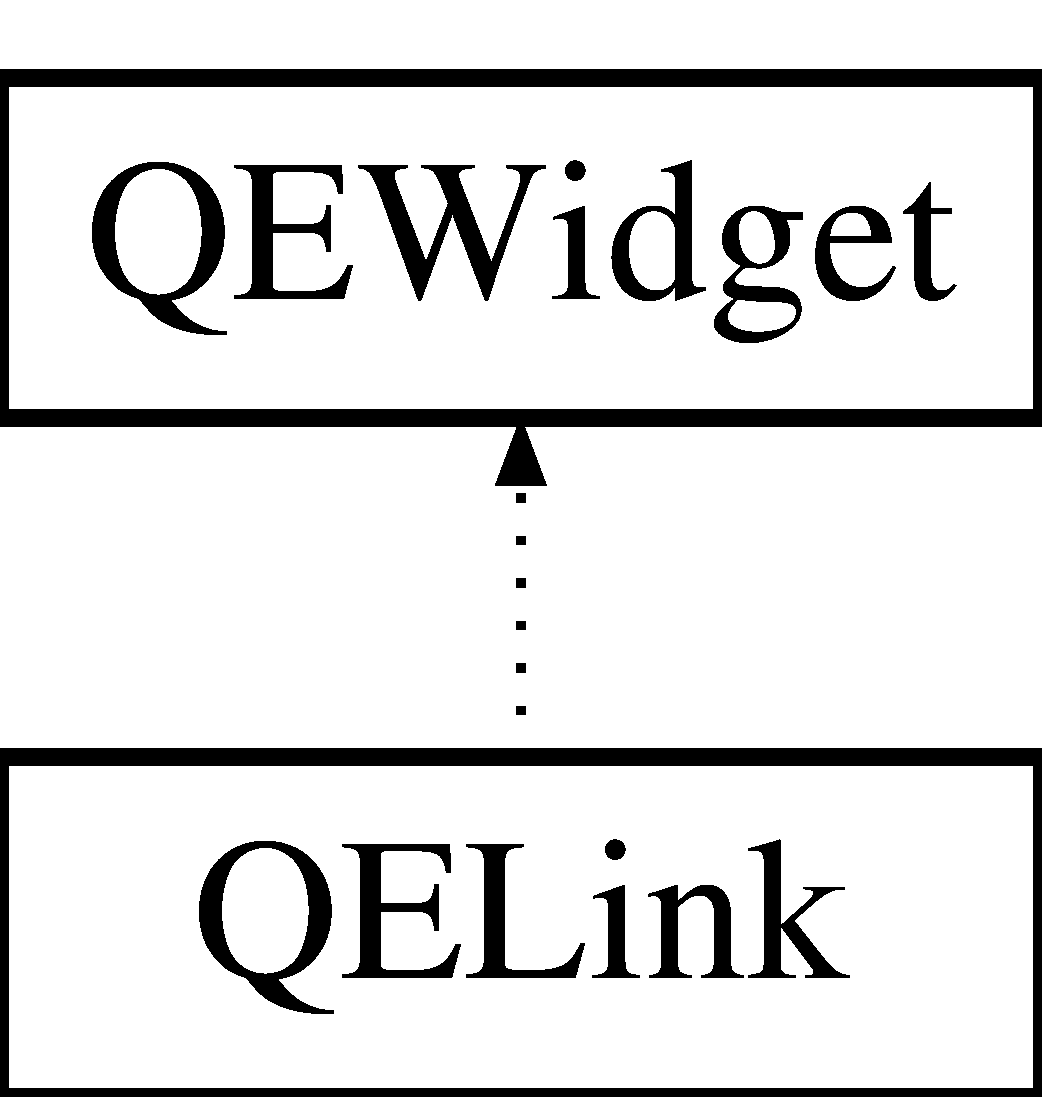
\includegraphics[height=2.000000cm]{classQELink}
\end{center}
\end{figure}
\subsection*{Public Types}
\begin{DoxyCompactItemize}
\item 
enum {\bfseries conditions} \{ \par
{\bfseries CONDITION\_\-EQ}, 
{\bfseries CONDITION\_\-NE}, 
{\bfseries CONDITION\_\-GT}, 
{\bfseries CONDITION\_\-GE}, 
\par
{\bfseries CONDITION\_\-LT}, 
{\bfseries CONDITION\_\-LE}
 \}
\item 
enum {\bfseries ConditionNames} \{ \par
{\bfseries Equal} =  QELink::CONDITION\_\-EQ, 
{\bfseries NotEqual} =  QELink::CONDITION\_\-NE, 
{\bfseries GreaterThan} =  QELink::CONDITION\_\-GT, 
{\bfseries GreaterThanOrEqual} =  QELink::CONDITION\_\-GE, 
\par
{\bfseries LessThan} =  QELink::CONDITION\_\-LT, 
{\bfseries LessThanOrEqual} =  QELink::CONDITION\_\-LE
 \}
\end{DoxyCompactItemize}
\subsection*{Public Slots}
\begin{DoxyCompactItemize}
\item 
\hypertarget{classQELink_ab34528168fc1e2030212ac0d249ce3c7}{
void {\bfseries in} (const bool \&in)}
\label{classQELink_ab34528168fc1e2030212ac0d249ce3c7}

\item 
\hypertarget{classQELink_a38ae1392e7774502c80728a81771f879}{
void {\bfseries in} (const qlonglong \&in)}
\label{classQELink_a38ae1392e7774502c80728a81771f879}

\item 
\hypertarget{classQELink_aba549d32f48240d619667b2078aa7878}{
void {\bfseries in} (const double \&in)}
\label{classQELink_aba549d32f48240d619667b2078aa7878}

\item 
\hypertarget{classQELink_ae635a10a35878aa8b36f61162288005e}{
void {\bfseries in} (const QString \&in)}
\label{classQELink_ae635a10a35878aa8b36f61162288005e}

\item 
\hypertarget{classQELink_ab54cbbfe1177ee623a990e408cb3e904}{
void {\bfseries autoFillBackground} (const bool \&enable)}
\label{classQELink_ab54cbbfe1177ee623a990e408cb3e904}

\end{DoxyCompactItemize}
\subsection*{Signals}
\begin{DoxyCompactItemize}
\item 
\hypertarget{classQELink_a4146b853a4ba30220f489d977498bb6a}{
void {\bfseries out} (const bool \&out)}
\label{classQELink_a4146b853a4ba30220f489d977498bb6a}

\item 
\hypertarget{classQELink_a82c149a101980f3959fe38b87e1f6859}{
void {\bfseries out} (const qlonglong \&out)}
\label{classQELink_a82c149a101980f3959fe38b87e1f6859}

\item 
\hypertarget{classQELink_a17c74630163d08c94bbcc058a1c5f19c}{
void {\bfseries out} (const double \&out)}
\label{classQELink_a17c74630163d08c94bbcc058a1c5f19c}

\item 
\hypertarget{classQELink_ac765dc648d35f6fb0ad748dfd0afd56a}{
void {\bfseries out} (const QString \&out)}
\label{classQELink_ac765dc648d35f6fb0ad748dfd0afd56a}

\end{DoxyCompactItemize}
\subsection*{Public Member Functions}
\begin{DoxyCompactItemize}
\item 
\hypertarget{classQELink_a56ae044b914e04a190c0237444c25647}{
{\bfseries QELink} (QWidget $\ast$parent=0)}
\label{classQELink_a56ae044b914e04a190c0237444c25647}

\item 
\hypertarget{classQELink_a498f2e13f229635aa336564de59c2b98}{
void {\bfseries setCondition} (conditions conditionIn)}
\label{classQELink_a498f2e13f229635aa336564de59c2b98}

\item 
\hypertarget{classQELink_a1511bf385fd4dcf16eb9eae84f271ebc}{
conditions {\bfseries getCondition} ()}
\label{classQELink_a1511bf385fd4dcf16eb9eae84f271ebc}

\item 
\hypertarget{classQELink_aa9972a078979919b7f4318f98f35b48a}{
void {\bfseries setComparisonValue} (QString comparisonValue)}
\label{classQELink_aa9972a078979919b7f4318f98f35b48a}

\item 
\hypertarget{classQELink_a3fff45bbdbfb47515acbaff93787c80c}{
QString {\bfseries getComparisonValue} ()}
\label{classQELink_a3fff45bbdbfb47515acbaff93787c80c}

\item 
\hypertarget{classQELink_a6d14898770aeffb90d467a00098642ea}{
void {\bfseries setSignalTrue} (bool signalTrue)}
\label{classQELink_a6d14898770aeffb90d467a00098642ea}

\item 
\hypertarget{classQELink_a3966ea0fc0445fec9a482ad2322dabd4}{
bool {\bfseries getSignalTrue} ()}
\label{classQELink_a3966ea0fc0445fec9a482ad2322dabd4}

\item 
\hypertarget{classQELink_a7074b2d0ec3bfddaec6ed8265278c6dc}{
void {\bfseries setSignalFalse} (bool signalFalse)}
\label{classQELink_a7074b2d0ec3bfddaec6ed8265278c6dc}

\item 
\hypertarget{classQELink_a0856b8b6f754c9847a0da8aa1139ef52}{
bool {\bfseries getSignalFalse} ()}
\label{classQELink_a0856b8b6f754c9847a0da8aa1139ef52}

\item 
\hypertarget{classQELink_a83e2b8e30c0f7fca3b1d7acb82c65d21}{
void {\bfseries setOutTrueValue} (QString outTrueValue)}
\label{classQELink_a83e2b8e30c0f7fca3b1d7acb82c65d21}

\item 
\hypertarget{classQELink_abfae26abac122ab582aca59b16c87dbc}{
QString {\bfseries getOutTrueValue} ()}
\label{classQELink_abfae26abac122ab582aca59b16c87dbc}

\item 
\hypertarget{classQELink_aeea7e9b1df802527e631e076e98f162e}{
void {\bfseries setOutFalseValue} (QString outFalseValue)}
\label{classQELink_aeea7e9b1df802527e631e076e98f162e}

\item 
\hypertarget{classQELink_af067479aaf906b5ba76a5bf892b95c8d}{
QString {\bfseries getOutFalseValue} ()}
\label{classQELink_af067479aaf906b5ba76a5bf892b95c8d}

\item 
\hypertarget{classQELink_af6d88bf370239426e333b8d45c8348af}{
void {\bfseries setRunVisible} (bool visibleIn)}
\label{classQELink_af6d88bf370239426e333b8d45c8348af}

\item 
\hypertarget{classQELink_a6735abb53f7b260809b0435e25602e43}{
bool {\bfseries getRunVisible} ()}
\label{classQELink_a6735abb53f7b260809b0435e25602e43}

\item 
\hypertarget{classQELink_a1266b86af77514105646113a36cd87f4}{
void {\bfseries setConditionProperty} (ConditionNames condition)}
\label{classQELink_a1266b86af77514105646113a36cd87f4}

\item 
\hypertarget{classQELink_a34317106f66b940c2f66b8fa007cd5c9}{
ConditionNames {\bfseries getConditionProperty} ()}
\label{classQELink_a34317106f66b940c2f66b8fa007cd5c9}

\end{DoxyCompactItemize}
\subsection*{Protected Attributes}
\begin{DoxyCompactItemize}
\item 
\hypertarget{classQELink_a13e17b9b474855b6e62789823e0b6ff0}{
conditions {\bfseries condition}}
\label{classQELink_a13e17b9b474855b6e62789823e0b6ff0}

\item 
\hypertarget{classQELink_a2284b564d555349cdde33a26f22a6b00}{
QVariant {\bfseries comparisonValue}}
\label{classQELink_a2284b564d555349cdde33a26f22a6b00}

\item 
\hypertarget{classQELink_aa6dfff5a2a6161cd3e71aa35524a41ad}{
bool {\bfseries signalTrue}}
\label{classQELink_aa6dfff5a2a6161cd3e71aa35524a41ad}

\item 
\hypertarget{classQELink_adface5dcb4029e7fa9c598e6a99ec9a0}{
bool {\bfseries signalFalse}}
\label{classQELink_adface5dcb4029e7fa9c598e6a99ec9a0}

\item 
\hypertarget{classQELink_a02dc407e1f9cbea2e819729b48539c04}{
QVariant {\bfseries outTrueValue}}
\label{classQELink_a02dc407e1f9cbea2e819729b48539c04}

\item 
\hypertarget{classQELink_aa08948f9296695ec066a993f19dedd80}{
QVariant {\bfseries outFalseValue}}
\label{classQELink_aa08948f9296695ec066a993f19dedd80}

\item 
\hypertarget{classQELink_a299abea79c3855a94d743e3540921a92}{
bool {\bfseries visible}}
\label{classQELink_a299abea79c3855a94d743e3540921a92}

\end{DoxyCompactItemize}
\subsection*{Properties}
\begin{DoxyCompactItemize}
\item 
\hypertarget{classQELink_a9d8a7d0a2e3e8e1990e39744421a769b}{
ConditionNames {\bfseries condition}}
\label{classQELink_a9d8a7d0a2e3e8e1990e39744421a769b}

\item 
\hypertarget{classQELink_a75adbd0ae5580f403a85ae26f4d4c7f7}{
QString {\bfseries comparisonValue}}
\label{classQELink_a75adbd0ae5580f403a85ae26f4d4c7f7}

\item 
\hypertarget{classQELink_a91959ab634890a3cbeba69f3ae5109a7}{
QString {\bfseries outTrueValue}}
\label{classQELink_a91959ab634890a3cbeba69f3ae5109a7}

\item 
\hypertarget{classQELink_a88c1b378fe7d57781432653b4cbb0055}{
QString {\bfseries outFalseValue}}
\label{classQELink_a88c1b378fe7d57781432653b4cbb0055}

\item 
\hypertarget{classQELink_a1a5c3bd9c25bc7bade374f574d2db3e0}{
bool {\bfseries runVisible}}
\label{classQELink_a1a5c3bd9c25bc7bade374f574d2db3e0}

\end{DoxyCompactItemize}


The documentation for this class was generated from the following files:\begin{DoxyCompactItemize}
\item 
/tmp/epicsqt/trunk/framework/widgets/QELink/QELink.h\item 
/tmp/epicsqt/trunk/framework/widgets/QELink/QELink.cpp\end{DoxyCompactItemize}

\hypertarget{classQELocalEnumeration}{
\section{QELocalEnumeration Class Reference}
\label{classQELocalEnumeration}\index{QELocalEnumeration@{QELocalEnumeration}}
}


{\ttfamily \#include $<$QELocalEnumeration.h$>$}

\subsection*{Classes}
\begin{DoxyCompactItemize}
\item 
class {\bfseries localEnumerationItem}
\end{DoxyCompactItemize}
\subsection*{Public Member Functions}
\begin{DoxyCompactItemize}
\item 
\hyperlink{classQELocalEnumeration_ac2d9d220a4cf1bfdf117794ce8f5bdfe}{QELocalEnumeration} ()
\item 
\hyperlink{classQELocalEnumeration_aa25091ab008116b2c147637d60655bb2}{QELocalEnumeration} (const QString \&localEnumeration)
\item 
void \hyperlink{classQELocalEnumeration_a02c88ef391172ffa14ef28e97b97b1b6}{setLocalEnumeration} (const QString \&localEnumeration)
\item 
QString \hyperlink{classQELocalEnumeration_af879ad170bcd0a34ec5368fbe7a87248}{getLocalEnumeration} ()
\item 
bool \hyperlink{classQELocalEnumeration_ac403a3f983934abdfccc0aeeae8b5e99}{isDefined} ()
\item 
QString \hyperlink{classQELocalEnumeration_a90694b2cbede83e31e17d49508b38488}{valueToText} (const QVariant \&value, bool \&match)
\item 
QVariant \hyperlink{classQELocalEnumeration_ad978d0739cba24df376beb290f1ec4a8}{textToValue} (const QString \&text, bool \&ok)
\item 
int \hyperlink{classQELocalEnumeration_aea4fd8ef2e8379c9f78901b7fb1fd548}{textToInt} (const QString \&text, bool \&ok)
\item 
double \hyperlink{classQELocalEnumeration_aa0060a5549c456f4d995b531b0797cdf}{textToDouble} (const QString \&text, bool \&ok)
\end{DoxyCompactItemize}


\subsection{Detailed Description}
This class allows a user defined two-\/way value to enumeration map. The map is define using a single string, typically a widget property string. This may then be used to replace the enumeration values provided by EPICS and/or provide an enueration set of more that 16 values. See \hyperlink{classQELocalEnumeration_a02c88ef391172ffa14ef28e97b97b1b6}{setLocalEnumeration()} for the use of 'localEnumeration'.

This functionality that this class provided was formerly embedded within \hyperlink{classQEStringFormatting}{QEStringFormatting}. 

\subsection{Constructor \& Destructor Documentation}
\hypertarget{classQELocalEnumeration_ac2d9d220a4cf1bfdf117794ce8f5bdfe}{
\index{QELocalEnumeration@{QELocalEnumeration}!QELocalEnumeration@{QELocalEnumeration}}
\index{QELocalEnumeration@{QELocalEnumeration}!QELocalEnumeration@{QELocalEnumeration}}
\subsubsection[{QELocalEnumeration}]{\setlength{\rightskip}{0pt plus 5cm}QELocalEnumeration::QELocalEnumeration (
\begin{DoxyParamCaption}
{}
\end{DoxyParamCaption}
)}}
\label{classQELocalEnumeration_ac2d9d220a4cf1bfdf117794ce8f5bdfe}
Constructors \hypertarget{classQELocalEnumeration_aa25091ab008116b2c147637d60655bb2}{
\index{QELocalEnumeration@{QELocalEnumeration}!QELocalEnumeration@{QELocalEnumeration}}
\index{QELocalEnumeration@{QELocalEnumeration}!QELocalEnumeration@{QELocalEnumeration}}
\subsubsection[{QELocalEnumeration}]{\setlength{\rightskip}{0pt plus 5cm}QELocalEnumeration::QELocalEnumeration (
\begin{DoxyParamCaption}
\item[{const QString \&}]{localEnumeration}
\end{DoxyParamCaption}
)}}
\label{classQELocalEnumeration_aa25091ab008116b2c147637d60655bb2}
Constructor with localEnumeration 

\subsection{Member Function Documentation}
\hypertarget{classQELocalEnumeration_af879ad170bcd0a34ec5368fbe7a87248}{
\index{QELocalEnumeration@{QELocalEnumeration}!getLocalEnumeration@{getLocalEnumeration}}
\index{getLocalEnumeration@{getLocalEnumeration}!QELocalEnumeration@{QELocalEnumeration}}
\subsubsection[{getLocalEnumeration}]{\setlength{\rightskip}{0pt plus 5cm}QString QELocalEnumeration::getLocalEnumeration (
\begin{DoxyParamCaption}
{}
\end{DoxyParamCaption}
)}}
\label{classQELocalEnumeration_af879ad170bcd0a34ec5368fbe7a87248}
Get the local enumeration strings. See \hyperlink{classQELocalEnumeration_a02c88ef391172ffa14ef28e97b97b1b6}{setLocalEnumeration()} for the use of 'localEnumeration'. \hypertarget{classQELocalEnumeration_ac403a3f983934abdfccc0aeeae8b5e99}{
\index{QELocalEnumeration@{QELocalEnumeration}!isDefined@{isDefined}}
\index{isDefined@{isDefined}!QELocalEnumeration@{QELocalEnumeration}}
\subsubsection[{isDefined}]{\setlength{\rightskip}{0pt plus 5cm}bool QELocalEnumeration::isDefined (
\begin{DoxyParamCaption}
{}
\end{DoxyParamCaption}
)}}
\label{classQELocalEnumeration_ac403a3f983934abdfccc0aeeae8b5e99}
Evaluates: getLocalEnumeration.count() $>$ 0 \hypertarget{classQELocalEnumeration_a02c88ef391172ffa14ef28e97b97b1b6}{
\index{QELocalEnumeration@{QELocalEnumeration}!setLocalEnumeration@{setLocalEnumeration}}
\index{setLocalEnumeration@{setLocalEnumeration}!QELocalEnumeration@{QELocalEnumeration}}
\subsubsection[{setLocalEnumeration}]{\setlength{\rightskip}{0pt plus 5cm}void QELocalEnumeration::setLocalEnumeration (
\begin{DoxyParamCaption}
\item[{const QString \&}]{localEnumeration}
\end{DoxyParamCaption}
)}}
\label{classQELocalEnumeration_a02c88ef391172ffa14ef28e97b97b1b6}
Parse the local enumeration string.

Format is:

\mbox{[}\mbox{[}$<$$|$$<$=$|$=$|$!=$|$$>$=$|$$>$\mbox{]}value1$|$$\ast$\mbox{]} : string1 , \mbox{[}\mbox{[}$<$$|$$<$=$|$=$|$!=$|$$>$=$|$$>$\mbox{]}value2$|$$\ast$\mbox{]} : string2 , \mbox{[}\mbox{[}$<$$|$$<$=$|$=$|$!=$|$$>$=$|$$>$\mbox{]}value3$|$$\ast$\mbox{]} : string3 , ...

Where: $<$ Less than $<$= Less than or equal = Equal (default if no operator specified) $>$= Greather than or equal $>$ Greater than Always match (used to specify default text)

Values may be numeric or textual Values do not have to be in any order, but first match wins Values may be quoted Strings may be quoted Consecutive values do not have to be present. Operator is assumed to be equality if not present. White space is ignored except within quoted strings. \par
 may be included in a string to indicate a line break

Examples are:

0:Off,1:On 0 : \char`\"{}Pump Running\char`\"{}, 1 : \char`\"{}Pump not running\char`\"{} 0:\char`\"{}\char`\"{}, 1:\char`\"{}Warning!$\backslash$nAlarm\char`\"{} $<$2:\char`\"{}Value is less than two\char`\"{}, =2:\char`\"{}Value is equal to two\char`\"{}, $>$2:\char`\"{}Value is grater than 2\char`\"{} 3:\char`\"{}Beamline Available\char`\"{}, $\ast$:\char`\"{}\char`\"{} \char`\"{}Pump Off\char`\"{}:\char`\"{}OH NO!, the pump is OFF!\char`\"{},\char`\"{}Pump On\char`\"{}:\char`\"{}It's OK, the pump is on\char`\"{}

The data value is converted to a string if no enumeration for that value is available. For example, if the local enumeration is '0:off,1:on', and a value of 10 is processed, the text generated is '10'. If a blank string is required, this should be explicit. for example, '0:off,1:on,10:\char`\"{}\char`\"{}'

A range of numbers can be covered by a pair of values as in the following example: $>$=4:\char`\"{}Between 4 and 8\char`\"{},$<$=8:\char`\"{}Between 4 and 8\char`\"{}

Will completely re-\/initialises the object. \hypertarget{classQELocalEnumeration_aa0060a5549c456f4d995b531b0797cdf}{
\index{QELocalEnumeration@{QELocalEnumeration}!textToDouble@{textToDouble}}
\index{textToDouble@{textToDouble}!QELocalEnumeration@{QELocalEnumeration}}
\subsubsection[{textToDouble}]{\setlength{\rightskip}{0pt plus 5cm}double QELocalEnumeration::textToDouble (
\begin{DoxyParamCaption}
\item[{const QString \&}]{text, }
\item[{bool \&}]{ok}
\end{DoxyParamCaption}
)}}
\label{classQELocalEnumeration_aa0060a5549c456f4d995b531b0797cdf}
Generate a double value given a string, using formatting defined within this class. If the value can be formatted the formatted value is returned and 'ok' is true. If the value can't be formatted then 0.0 is returned and 'ok' is false. \hypertarget{classQELocalEnumeration_aea4fd8ef2e8379c9f78901b7fb1fd548}{
\index{QELocalEnumeration@{QELocalEnumeration}!textToInt@{textToInt}}
\index{textToInt@{textToInt}!QELocalEnumeration@{QELocalEnumeration}}
\subsubsection[{textToInt}]{\setlength{\rightskip}{0pt plus 5cm}int QELocalEnumeration::textToInt (
\begin{DoxyParamCaption}
\item[{const QString \&}]{text, }
\item[{bool \&}]{ok}
\end{DoxyParamCaption}
)}}
\label{classQELocalEnumeration_aea4fd8ef2e8379c9f78901b7fb1fd548}
Generate an integer value given a string, using formatting defined within this class. If the value can be formatted the formatted value is returned and 'ok' is true. If the value can't be formatted then 0 is returned and 'ok' is false. \hypertarget{classQELocalEnumeration_ad978d0739cba24df376beb290f1ec4a8}{
\index{QELocalEnumeration@{QELocalEnumeration}!textToValue@{textToValue}}
\index{textToValue@{textToValue}!QELocalEnumeration@{QELocalEnumeration}}
\subsubsection[{textToValue}]{\setlength{\rightskip}{0pt plus 5cm}QVariant QELocalEnumeration::textToValue (
\begin{DoxyParamCaption}
\item[{const QString \&}]{text, }
\item[{bool \&}]{ok}
\end{DoxyParamCaption}
)}}
\label{classQELocalEnumeration_ad978d0739cba24df376beb290f1ec4a8}
Generate a value given a string, using formatting defined within this class. If the value can be formatted the formatted value is returned and 'ok' is true. If the value can't be formatted an error string is returned and 'ok' is false \hypertarget{classQELocalEnumeration_a90694b2cbede83e31e17d49508b38488}{
\index{QELocalEnumeration@{QELocalEnumeration}!valueToText@{valueToText}}
\index{valueToText@{valueToText}!QELocalEnumeration@{QELocalEnumeration}}
\subsubsection[{valueToText}]{\setlength{\rightskip}{0pt plus 5cm}QString QELocalEnumeration::valueToText (
\begin{DoxyParamCaption}
\item[{const QVariant \&}]{value, }
\item[{bool \&}]{match}
\end{DoxyParamCaption}
)}}
\label{classQELocalEnumeration_a90694b2cbede83e31e17d49508b38488}
Format a variant value using local enumeration list. If the value is numeric, then the value is compared to the numeric interpretation of the enumeration values, if the value is textual, then the value is compared to the textual enumeration values. 

The documentation for this class was generated from the following files:\begin{DoxyCompactItemize}
\item 
/tmp/epicsqt/trunk/framework/data/include/QELocalEnumeration.h\item 
/tmp/epicsqt/trunk/framework/data/src/QELocalEnumeration.cpp\end{DoxyCompactItemize}

\hypertarget{classQELog}{
\section{QELog Class Reference}
\label{classQELog}\index{QELog@{QELog}}
}
Inheritance diagram for QELog:\begin{figure}[H]
\begin{center}
\leavevmode
\includegraphics[height=2.204725cm]{classQELog}
\end{center}
\end{figure}
\subsection*{Public Types}
\begin{DoxyCompactItemize}
\item 
enum {\bfseries detailsLayoutProperty} \{ {\bfseries Top} =  TOP, 
{\bfseries Bottom} =  BOTTOM, 
{\bfseries Left} =  LEFT, 
{\bfseries Right} =  RIGHT
 \}
\item 
enum {\bfseries MessageFilterOptions} \{ {\bfseries Any} =  UserMessage::MESSAGE\_\-FILTER\_\-ANY, 
{\bfseries Match} =  UserMessage::MESSAGE\_\-FILTER\_\-MATCH, 
{\bfseries None} =  UserMessage::MESSAGE\_\-FILTER\_\-NONE
 \}
\end{DoxyCompactItemize}
\subsection*{Public Member Functions}
\begin{DoxyCompactItemize}
\item 
\hypertarget{classQELog_ab8dfcf853cd616c4b3ff0871d0a9fed2}{
{\bfseries QELog} (QWidget $\ast$pParent=0)}
\label{classQELog_ab8dfcf853cd616c4b3ff0871d0a9fed2}

\item 
\hypertarget{classQELog_a44b59d902bf4a224a6f3b17f44c5d1ee}{
void {\bfseries setShowColumnTime} (bool pValue)}
\label{classQELog_a44b59d902bf4a224a6f3b17f44c5d1ee}

\item 
\hypertarget{classQELog_a101275b6828073b8549d5afbd6fde0f4}{
bool {\bfseries getShowColumnTime} ()}
\label{classQELog_a101275b6828073b8549d5afbd6fde0f4}

\item 
\hypertarget{classQELog_a863a48002251e5ffd14fdda865999880}{
void {\bfseries setShowColumnType} (bool pValue)}
\label{classQELog_a863a48002251e5ffd14fdda865999880}

\item 
\hypertarget{classQELog_aca7fdc600f38febe8d3981dca10bdfbe}{
bool {\bfseries getShowColumnType} ()}
\label{classQELog_aca7fdc600f38febe8d3981dca10bdfbe}

\item 
\hypertarget{classQELog_a72b6bac93761df396df2182035cea478}{
void {\bfseries setShowColumnMessage} (bool pValue)}
\label{classQELog_a72b6bac93761df396df2182035cea478}

\item 
\hypertarget{classQELog_ad4d869b164c31296834be96704a856e2}{
bool {\bfseries getShowColumnMessage} ()}
\label{classQELog_ad4d869b164c31296834be96704a856e2}

\item 
\hypertarget{classQELog_abd19f741eed9698ecfec6fe974591dc4}{
void {\bfseries setShowMessageFilter} (bool pValue)}
\label{classQELog_abd19f741eed9698ecfec6fe974591dc4}

\item 
\hypertarget{classQELog_a02b535f7c8cc3852eb507fb0f693e532}{
bool {\bfseries getShowMessageFilter} ()}
\label{classQELog_a02b535f7c8cc3852eb507fb0f693e532}

\item 
\hypertarget{classQELog_a0db8ebcef66219fced74de0c68f00216}{
void {\bfseries setShowClear} (bool pValue)}
\label{classQELog_a0db8ebcef66219fced74de0c68f00216}

\item 
\hypertarget{classQELog_a134039567e973301ef469e3effc1a168}{
bool {\bfseries getShowClear} ()}
\label{classQELog_a134039567e973301ef469e3effc1a168}

\item 
\hypertarget{classQELog_a6d284ca7fee43fcdfcf8c0f7e780fad6}{
void {\bfseries setShowSave} (bool pValue)}
\label{classQELog_a6d284ca7fee43fcdfcf8c0f7e780fad6}

\item 
\hypertarget{classQELog_a2e7a396cd52d23d2ad4b5ba6238aec2b}{
bool {\bfseries getShowSave} ()}
\label{classQELog_a2e7a396cd52d23d2ad4b5ba6238aec2b}

\item 
\hypertarget{classQELog_a5c762bcd55b11bf4ffe0294e10a59e33}{
void {\bfseries setDetailsLayout} (int pValue)}
\label{classQELog_a5c762bcd55b11bf4ffe0294e10a59e33}

\item 
\hypertarget{classQELog_ac7beaaef82e263744eae47f5f1cde4ae}{
int {\bfseries getDetailsLayout} ()}
\label{classQELog_ac7beaaef82e263744eae47f5f1cde4ae}

\item 
\hypertarget{classQELog_a98ca811e5b75f0be827b80f307537f5e}{
void {\bfseries setScrollToBottom} (bool pValue)}
\label{classQELog_a98ca811e5b75f0be827b80f307537f5e}

\item 
\hypertarget{classQELog_a1e9d96a97129270f5eddd82c760aa965}{
bool {\bfseries getScrollToBottom} ()}
\label{classQELog_a1e9d96a97129270f5eddd82c760aa965}

\item 
\hypertarget{classQELog_a6771e6806cb1152d55d7314814666e2c}{
void {\bfseries setInfoColor} (QColor pValue)}
\label{classQELog_a6771e6806cb1152d55d7314814666e2c}

\item 
\hypertarget{classQELog_a65c4ca881ac4c0c36e5aa92c147516e6}{
QColor {\bfseries getInfoColor} ()}
\label{classQELog_a65c4ca881ac4c0c36e5aa92c147516e6}

\item 
\hypertarget{classQELog_ab064d5949b9f386af8a2777121734a41}{
void {\bfseries setWarningColor} (QColor pValue)}
\label{classQELog_ab064d5949b9f386af8a2777121734a41}

\item 
\hypertarget{classQELog_a71790e5ac0d3070b3006313fb361b90a}{
QColor {\bfseries getWarningColor} ()}
\label{classQELog_a71790e5ac0d3070b3006313fb361b90a}

\item 
\hypertarget{classQELog_a4848bc1ff1fd76a40c16cba3048902dd}{
void {\bfseries setErrorColor} (QColor pValue)}
\label{classQELog_a4848bc1ff1fd76a40c16cba3048902dd}

\item 
\hypertarget{classQELog_a74203f1bf43dc7ec900cd3d9c86e116f}{
QColor {\bfseries getErrorColor} ()}
\label{classQELog_a74203f1bf43dc7ec900cd3d9c86e116f}

\item 
\hypertarget{classQELog_affdc407f650d6ff293c1846f393f6fcf}{
void {\bfseries clearLog} ()}
\label{classQELog_affdc407f650d6ff293c1846f393f6fcf}

\item 
\hypertarget{classQELog_a2ae53a6c4421682bc2402f41cf99a68f}{
void {\bfseries addLog} (int pType, QString pMessage)}
\label{classQELog_a2ae53a6c4421682bc2402f41cf99a68f}

\item 
\hypertarget{classQELog_a69a3dd36bc19a839367d5b9bcc307c53}{
void {\bfseries refreshLog} ()}
\label{classQELog_a69a3dd36bc19a839367d5b9bcc307c53}

\item 
\hypertarget{classQELog_a7c3c8ff38b8597693761bd5f6c61d1a5}{
void {\bfseries setDetailsLayoutProperty} (detailsLayoutProperty pDetailsLayout)}
\label{classQELog_a7c3c8ff38b8597693761bd5f6c61d1a5}

\item 
\hypertarget{classQELog_ac4bf3c55033e43e97eeb2b57af37c010}{
detailsLayoutProperty {\bfseries getDetailsLayoutProperty} ()}
\label{classQELog_ac4bf3c55033e43e97eeb2b57af37c010}

\item 
\hypertarget{classQELog_aed7337e1e608fc3a3c9f1f6c16d07419}{
MessageFilterOptions {\bfseries getMessageFormFilter} ()}
\label{classQELog_aed7337e1e608fc3a3c9f1f6c16d07419}

\item 
\hypertarget{classQELog_a4960709b235e912483140369a40fc076}{
void {\bfseries setMessageFormFilter} (MessageFilterOptions messageFormFilter)}
\label{classQELog_a4960709b235e912483140369a40fc076}

\item 
\hypertarget{classQELog_a6072239eb36c73492dc8456a1fbddca5}{
MessageFilterOptions {\bfseries getMessageSourceFilter} ()}
\label{classQELog_a6072239eb36c73492dc8456a1fbddca5}

\item 
\hypertarget{classQELog_ab2a7190148ef19a798589eafbd00b1a1}{
void {\bfseries setMessageSourceFilter} (MessageFilterOptions messageSourceFilter)}
\label{classQELog_ab2a7190148ef19a798589eafbd00b1a1}

\end{DoxyCompactItemize}
\subsection*{Protected Attributes}
\begin{DoxyCompactItemize}
\item 
\hypertarget{classQELog_af777a0bf10d169f067db5f8cc30ab36b}{
\hyperlink{class__QTableWidgetLog}{\_\-QTableWidgetLog} $\ast$ {\bfseries qTableWidgetLog}}
\label{classQELog_af777a0bf10d169f067db5f8cc30ab36b}

\item 
\hypertarget{classQELog_aae55b98c54f90af7407266a5b51980b1}{
QCheckBox $\ast$ {\bfseries qCheckBoxInfoMessage}}
\label{classQELog_aae55b98c54f90af7407266a5b51980b1}

\item 
\hypertarget{classQELog_a4912b66605b4070917002561bbe8542a}{
QCheckBox $\ast$ {\bfseries qCheckBoxWarningMessage}}
\label{classQELog_a4912b66605b4070917002561bbe8542a}

\item 
\hypertarget{classQELog_af794a6ac311b31900f9040f6cd9801e9}{
QCheckBox $\ast$ {\bfseries qCheckBoxErrorMessage}}
\label{classQELog_af794a6ac311b31900f9040f6cd9801e9}

\item 
\hypertarget{classQELog_a364e8307f60739053bfdf07e4ddce99d}{
QPushButton $\ast$ {\bfseries qPushButtonClear}}
\label{classQELog_a364e8307f60739053bfdf07e4ddce99d}

\item 
\hypertarget{classQELog_ad2b0526aabf80a9715006a387672438f}{
QPushButton $\ast$ {\bfseries qPushButtonSave}}
\label{classQELog_ad2b0526aabf80a9715006a387672438f}

\item 
\hypertarget{classQELog_a5e48b41a339d171df6ef7ebc27236d56}{
QColor {\bfseries qColorInfo}}
\label{classQELog_a5e48b41a339d171df6ef7ebc27236d56}

\item 
\hypertarget{classQELog_a04869b854c9b40cf69b65d0d8d1a621c}{
QColor {\bfseries qColorWarning}}
\label{classQELog_a04869b854c9b40cf69b65d0d8d1a621c}

\item 
\hypertarget{classQELog_a8a81427931a667eb7660164c055b829f}{
QColor {\bfseries qColorError}}
\label{classQELog_a8a81427931a667eb7660164c055b829f}

\item 
\hypertarget{classQELog_a3f5670503907fe9a6412d5cbf341419d}{
bool {\bfseries scrollToBottom}}
\label{classQELog_a3f5670503907fe9a6412d5cbf341419d}

\item 
\hypertarget{classQELog_a2e919dc42b8651e940433c6f0f91759f}{
int {\bfseries detailsLayout}}
\label{classQELog_a2e919dc42b8651e940433c6f0f91759f}

\end{DoxyCompactItemize}
\subsection*{Properties}
\begin{DoxyCompactItemize}
\item 
\hypertarget{classQELog_a499bb8355e2d19ec8ddb444752063b25}{
bool {\bfseries showColumnTime}}
\label{classQELog_a499bb8355e2d19ec8ddb444752063b25}

\item 
\hypertarget{classQELog_a4a9a0fb2694c019229bb94d9989bcd91}{
bool {\bfseries showColumnType}}
\label{classQELog_a4a9a0fb2694c019229bb94d9989bcd91}

\item 
\hypertarget{classQELog_ae74260abd3ea8861f0c6247eb1cfc65a}{
bool {\bfseries showColumnMessage}}
\label{classQELog_ae74260abd3ea8861f0c6247eb1cfc65a}

\item 
\hypertarget{classQELog_a8058526fed5816228e6bc81413b18cbf}{
bool {\bfseries showMessageFilter}}
\label{classQELog_a8058526fed5816228e6bc81413b18cbf}

\item 
\hypertarget{classQELog_a935a49a585c6cf41bf0b89a96a46f9f1}{
bool {\bfseries showClear}}
\label{classQELog_a935a49a585c6cf41bf0b89a96a46f9f1}

\item 
\hypertarget{classQELog_a67f5ae906b00e94c29b6915ceb4ce917}{
bool {\bfseries showSave}}
\label{classQELog_a67f5ae906b00e94c29b6915ceb4ce917}

\item 
\hypertarget{classQELog_af691c12d13564e2005a85d9054273aef}{
detailsLayoutProperty {\bfseries detailsLayout}}
\label{classQELog_af691c12d13564e2005a85d9054273aef}

\item 
\hypertarget{classQELog_a78bee8686487eaa81b562f45ad9d8f66}{
QColor {\bfseries infoColor}}
\label{classQELog_a78bee8686487eaa81b562f45ad9d8f66}

\item 
\hypertarget{classQELog_af14bb056d0e7cde60aba32b981ece445}{
QColor {\bfseries warningColor}}
\label{classQELog_af14bb056d0e7cde60aba32b981ece445}

\item 
\hypertarget{classQELog_af533b34ae4bab45db273a90223367725}{
QColor {\bfseries errorColor}}
\label{classQELog_af533b34ae4bab45db273a90223367725}

\item 
\hypertarget{classQELog_a63f3310fe80511374cb4028a0124e96c}{
MessageFilterOptions {\bfseries messageFormFilter}}
\label{classQELog_a63f3310fe80511374cb4028a0124e96c}

\item 
\hypertarget{classQELog_abcc2581abd947c209d4f86ad3bd7c720}{
MessageFilterOptions {\bfseries messageSourceFilter}}
\label{classQELog_abcc2581abd947c209d4f86ad3bd7c720}

\item 
\hypertarget{classQELog_a7e7692c580904d7dc097d9eff3dd071c}{
unsigned {\bfseries int}}
\label{classQELog_a7e7692c580904d7dc097d9eff3dd071c}

\end{DoxyCompactItemize}


The documentation for this class was generated from the following files:\begin{DoxyCompactItemize}
\item 
/tmp/epicsqt/trunk/framework/widgets/QELog/QELog.h\item 
/tmp/epicsqt/trunk/framework/widgets/QELog/QELog.cpp\end{DoxyCompactItemize}

\hypertarget{classQELogin}{
\section{QELogin Class Reference}
\label{classQELogin}\index{QELogin@{QELogin}}
}
Inheritance diagram for QELogin:\begin{figure}[H]
\begin{center}
\leavevmode
\includegraphics[height=2.204725cm]{classQELogin}
\end{center}
\end{figure}
\subsection*{Public Types}
\begin{DoxyCompactItemize}
\item 
enum {\bfseries userTypesProperty} \{ {\bfseries User} =  userLevelTypes::USERLEVEL\_\-USER, 
{\bfseries Scientist} =  userLevelTypes::USERLEVEL\_\-SCIENTIST, 
{\bfseries Engineer} =  userLevelTypes::USERLEVEL\_\-ENGINEER
 \}
\item 
enum {\bfseries detailsLayoutProperty} \{ {\bfseries Top} =  TOP, 
{\bfseries Bottom} =  BOTTOM, 
{\bfseries Left} =  LEFT, 
{\bfseries Right} =  RIGHT
 \}
\end{DoxyCompactItemize}
\subsection*{Public Member Functions}
\begin{DoxyCompactItemize}
\item 
\hypertarget{classQELogin_afb826421547c63a416768cb7f77ea8cc}{
QString {\bfseries getPriorityUserPassword} ()}
\label{classQELogin_afb826421547c63a416768cb7f77ea8cc}

\item 
\hypertarget{classQELogin_a587db3a2efe1c6719bc3e9712bca75bf}{
QString {\bfseries getPriorityScientistPassword} ()}
\label{classQELogin_a587db3a2efe1c6719bc3e9712bca75bf}

\item 
\hypertarget{classQELogin_a1f58b0cd0faf8ad9b523e373204d6682}{
QString {\bfseries getPriorityEngineerPassword} ()}
\label{classQELogin_a1f58b0cd0faf8ad9b523e373204d6682}

\item 
\hypertarget{classQELogin_a5524af2d70794e59b592bfa01edf8232}{
{\bfseries QELogin} (QWidget $\ast$pParent=0)}
\label{classQELogin_a5524af2d70794e59b592bfa01edf8232}

\item 
\hypertarget{classQELogin_af70c19c39cd68e148feb44ea3c3f478c}{
void {\bfseries setShowUserType} (bool pValue)}
\label{classQELogin_af70c19c39cd68e148feb44ea3c3f478c}

\item 
\hypertarget{classQELogin_a4ef5d7c71a38910b754727ba64bb2ab8}{
bool {\bfseries getShowUserType} ()}
\label{classQELogin_a4ef5d7c71a38910b754727ba64bb2ab8}

\item 
\hypertarget{classQELogin_a0928037edcac96a23f18d9e07f2200b5}{
void {\bfseries setShowLogin} (bool pValue)}
\label{classQELogin_a0928037edcac96a23f18d9e07f2200b5}

\item 
\hypertarget{classQELogin_adced91fe4807884e2056eeca262bcf0a}{
bool {\bfseries getShowButtonLogin} ()}
\label{classQELogin_adced91fe4807884e2056eeca262bcf0a}

\item 
\hypertarget{classQELogin_a9deee223b1abf3e02fc403c3f090603d}{
void {\bfseries setShowLogout} (bool pValue)}
\label{classQELogin_a9deee223b1abf3e02fc403c3f090603d}

\item 
\hypertarget{classQELogin_afb3ead74ebd447120bf3c139a35e5427}{
bool {\bfseries getShowButtonLogout} ()}
\label{classQELogin_afb3ead74ebd447120bf3c139a35e5427}

\item 
\hypertarget{classQELogin_a1910c8e940b45f5966b8bb1e43c14e75}{
void {\bfseries setUserPassword} (QString pValue)}
\label{classQELogin_a1910c8e940b45f5966b8bb1e43c14e75}

\item 
\hypertarget{classQELogin_a9590da0d1f298f1d7e1ae63aabce5689}{
QString {\bfseries getUserPassword} ()}
\label{classQELogin_a9590da0d1f298f1d7e1ae63aabce5689}

\item 
\hypertarget{classQELogin_a33e0e11e9e34248b39dc9c23a797f429}{
void {\bfseries setScientistPassword} (QString pValue)}
\label{classQELogin_a33e0e11e9e34248b39dc9c23a797f429}

\item 
\hypertarget{classQELogin_a7152963ebb09297f550f0a129cb77101}{
QString {\bfseries getScientistPassword} ()}
\label{classQELogin_a7152963ebb09297f550f0a129cb77101}

\item 
\hypertarget{classQELogin_afc734b2a8c5432946f3c6b1c7a245374}{
void {\bfseries setEngineerPassword} (QString pValue)}
\label{classQELogin_afc734b2a8c5432946f3c6b1c7a245374}

\item 
\hypertarget{classQELogin_afb3a491ee4a238e0896d8e6ad7afc875}{
QString {\bfseries getEngineerPassword} ()}
\label{classQELogin_afb3a491ee4a238e0896d8e6ad7afc875}

\item 
\hypertarget{classQELogin_a1cd337ccee3961e88412db959678f25b}{
void {\bfseries setCurrentUserType} (int pValue)}
\label{classQELogin_a1cd337ccee3961e88412db959678f25b}

\item 
\hypertarget{classQELogin_a628a4606503ae46dbf551b71dd26bd96}{
int {\bfseries getCurrentUserType} ()}
\label{classQELogin_a628a4606503ae46dbf551b71dd26bd96}

\item 
\hypertarget{classQELogin_af8aab36c993af312a43e5e2540d4ce2a}{
void {\bfseries setDetailsLayout} (int pValue)}
\label{classQELogin_af8aab36c993af312a43e5e2540d4ce2a}

\item 
\hypertarget{classQELogin_ae95902a9ce8e3c24f9404862e6ae63c3}{
int {\bfseries getDetailsLayout} ()}
\label{classQELogin_ae95902a9ce8e3c24f9404862e6ae63c3}

\item 
\hypertarget{classQELogin_ab36cce30019e22008cf1cd73a0aeb6dd}{
QString {\bfseries getUserTypeName} (\hyperlink{classuserLevelTypes_a033cf2a40f620286b1839dd360c8497b}{userLevelTypes::userLevels} type)}
\label{classQELogin_ab36cce30019e22008cf1cd73a0aeb6dd}

\item 
\hypertarget{classQELogin_a0cb38d4f6f4d761119874e9d196905bb}{
void {\bfseries logoutCurrentUserType} ()}
\label{classQELogin_a0cb38d4f6f4d761119874e9d196905bb}

\item 
\hypertarget{classQELogin_a666726d3a1378e92daa8f159e6a18b49}{
void {\bfseries setCurrentUserTypeProperty} (userTypesProperty pUserType)}
\label{classQELogin_a666726d3a1378e92daa8f159e6a18b49}

\item 
\hypertarget{classQELogin_a99033119aa0a5e58f05105a3532486a2}{
userTypesProperty {\bfseries getCurrentUserTypeProperty} ()}
\label{classQELogin_a99033119aa0a5e58f05105a3532486a2}

\item 
\hypertarget{classQELogin_a881e29f43cee185fb03a5d60c27d6483}{
void {\bfseries setDetailsLayoutProperty} (detailsLayoutProperty pDetailsLayout)}
\label{classQELogin_a881e29f43cee185fb03a5d60c27d6483}

\item 
\hypertarget{classQELogin_a9590edb8a86304008e5036710e4f95b2}{
detailsLayoutProperty {\bfseries getDetailsLayoutProperty} ()}
\label{classQELogin_a9590edb8a86304008e5036710e4f95b2}

\end{DoxyCompactItemize}
\subsection*{Protected Attributes}
\begin{DoxyCompactItemize}
\item 
\hypertarget{classQELogin_ac7d727ef13a9e1eec80a48f54c902a6c}{
QStack$<$ int $>$ {\bfseries loginHistory}}
\label{classQELogin_ac7d727ef13a9e1eec80a48f54c902a6c}

\item 
\hypertarget{classQELogin_a7e21b962c87c70b7533910472d0100ef}{
QPushButton $\ast$ {\bfseries qPushButtonLogin}}
\label{classQELogin_a7e21b962c87c70b7533910472d0100ef}

\item 
\hypertarget{classQELogin_ae7ade17f086d04d0b5bb1ef35dbc041b}{
QPushButton $\ast$ {\bfseries qPushButtonLogout}}
\label{classQELogin_ae7ade17f086d04d0b5bb1ef35dbc041b}

\item 
\hypertarget{classQELogin_a40d6529625f86de8c2c4edf069522992}{
QLabel $\ast$ {\bfseries qLabelUserType}}
\label{classQELogin_a40d6529625f86de8c2c4edf069522992}

\item 
\hypertarget{classQELogin_ae0ae55a4c3a19f20898b32bc4ef3df33}{
QString {\bfseries userPassword}}
\label{classQELogin_ae0ae55a4c3a19f20898b32bc4ef3df33}

\item 
\hypertarget{classQELogin_a48ac49245c600c3dbb9a0d052aafac26}{
QString {\bfseries scientistPassword}}
\label{classQELogin_a48ac49245c600c3dbb9a0d052aafac26}

\item 
\hypertarget{classQELogin_aee316604b82dabea914c7b084a1cb7a7}{
QString {\bfseries engineerPassword}}
\label{classQELogin_aee316604b82dabea914c7b084a1cb7a7}

\item 
\hypertarget{classQELogin_a11868fca0c9c3bc050377b1b1a36f34b}{
int {\bfseries currentUserType}}
\label{classQELogin_a11868fca0c9c3bc050377b1b1a36f34b}

\item 
\hypertarget{classQELogin_abfba9ddff05d536f6db0b36696fbe99f}{
int {\bfseries detailsLayout}}
\label{classQELogin_abfba9ddff05d536f6db0b36696fbe99f}

\end{DoxyCompactItemize}
\subsection*{Properties}
\begin{DoxyCompactItemize}
\item 
\hypertarget{classQELogin_a3b0cf0d664303b8e5518a794e519f9a1}{
bool {\bfseries showUserType}}
\label{classQELogin_a3b0cf0d664303b8e5518a794e519f9a1}

\item 
\hypertarget{classQELogin_a68b5126a1330359a1f1980750bfcbf2a}{
bool {\bfseries showLogin}}
\label{classQELogin_a68b5126a1330359a1f1980750bfcbf2a}

\item 
\hypertarget{classQELogin_a35af360423e3838aafeee71e6ec4e7b9}{
bool {\bfseries showLogout}}
\label{classQELogin_a35af360423e3838aafeee71e6ec4e7b9}

\item 
\hypertarget{classQELogin_a73ee001353e9f44af0926f55b59238c3}{
userTypesProperty {\bfseries currentUserType}}
\label{classQELogin_a73ee001353e9f44af0926f55b59238c3}

\item 
\hypertarget{classQELogin_a0af80091c57cba7f3673c8175b9224a5}{
detailsLayoutProperty {\bfseries detailsLayout}}
\label{classQELogin_a0af80091c57cba7f3673c8175b9224a5}

\end{DoxyCompactItemize}


The documentation for this class was generated from the following files:\begin{DoxyCompactItemize}
\item 
/tmp/epicsqt/trunk/framework/widgets/QELogin/QELogin.h\item 
/tmp/epicsqt/trunk/framework/widgets/QELogin/QELogin.cpp\end{DoxyCompactItemize}

\hypertarget{classQENumericEdit}{
\section{QENumericEdit Class Reference}
\label{classQENumericEdit}\index{QENumericEdit@{QENumericEdit}}
}


The \hyperlink{classQENumericEdit}{QENumericEdit} class This class is similar to \hyperlink{classQELineEdit}{QELineEdit} (both of which are derived from QLineEdit). However this class is tailored specifcially for editing numerical values.  




{\ttfamily \#include $<$QENumericEdit.h$>$}

Inheritance diagram for QENumericEdit:\begin{figure}[H]
\begin{center}
\leavevmode
\includegraphics[height=2.939633cm]{classQENumericEdit}
\end{center}
\end{figure}
\subsection*{Public Types}
\begin{DoxyCompactItemize}
\item 
enum \hyperlink{classQENumericEdit_a147ff9d9e547fe10391849a89f359223}{Radicies} \{ {\bfseries Decimal} =  0, 
{\bfseries Hexadecimal}, 
{\bfseries Octal}, 
{\bfseries Binary}
 \}
\begin{DoxyCompactList}\small\item\em Specify radix, default is Decimal. \end{DoxyCompactList}\item 
enum \hyperlink{classQENumericEdit_a42cabb099c034289576897ac0d8e89e0}{Separators} \{ {\bfseries None} =  0, 
{\bfseries Comma}, 
{\bfseries Underscore}, 
{\bfseries Space}
 \}
\begin{DoxyCompactList}\small\item\em Specify digit 'thousands' separator character, default is none. \end{DoxyCompactList}\end{DoxyCompactItemize}
\subsection*{Signals}
\begin{DoxyCompactItemize}
\item 
void \hyperlink{classQENumericEdit_a8126ea52eefb6613e06109a12003621e}{dbValueChanged} (const double \&out)
\end{DoxyCompactItemize}
\subsection*{Public Member Functions}
\begin{DoxyCompactItemize}
\item 
\hyperlink{classQENumericEdit_ab43a0c2bc70d13d8e01cb9d9a14cabf7}{QENumericEdit} (QWidget $\ast$parent=0)
\item 
\hyperlink{classQENumericEdit_a33d4a3b18bc0c55a533155bc625fd567}{QENumericEdit} (const QString \&variableName, QWidget $\ast$parent=0)
\item 
\hypertarget{classQENumericEdit_ad85eeaf0b4fe46addafa0ed812fcb367}{
virtual \hyperlink{classQENumericEdit_ad85eeaf0b4fe46addafa0ed812fcb367}{$\sim$QENumericEdit} ()}
\label{classQENumericEdit_ad85eeaf0b4fe46addafa0ed812fcb367}

\begin{DoxyCompactList}\small\item\em Destruction. \end{DoxyCompactList}\item 
\hypertarget{classQENumericEdit_a23a924d1ca4b23c279991391af45df72}{
double {\bfseries getNumericValue} ()}
\label{classQENumericEdit_a23a924d1ca4b23c279991391af45df72}

\end{DoxyCompactItemize}
\subsection*{Protected Member Functions}
\begin{DoxyCompactItemize}
\item 
\hypertarget{classQENumericEdit_a617ece9f34fdf00ac1ccf0fbeb7108a0}{
void {\bfseries setAutoScale} (const bool value)}
\label{classQENumericEdit_a617ece9f34fdf00ac1ccf0fbeb7108a0}

\item 
\hypertarget{classQENumericEdit_a549b328f435ae0e91d36e0a9d790f204}{
bool {\bfseries getAutoScale} ()}
\label{classQENumericEdit_a549b328f435ae0e91d36e0a9d790f204}

\item 
\hypertarget{classQENumericEdit_acf665f829b68397f7b6a10dd97a2353e}{
void {\bfseries setPropertyPrecision} (const int value)}
\label{classQENumericEdit_acf665f829b68397f7b6a10dd97a2353e}

\item 
\hypertarget{classQENumericEdit_ab9badbc5a5b875d4db34b70c23016ae5}{
int {\bfseries getPropertyPrecision} ()}
\label{classQENumericEdit_ab9badbc5a5b875d4db34b70c23016ae5}

\item 
\hypertarget{classQENumericEdit_a3cdb2bdb6cf4a9096bccc3e13c51df7e}{
void {\bfseries setPropertyLeadingZeros} (const int value)}
\label{classQENumericEdit_a3cdb2bdb6cf4a9096bccc3e13c51df7e}

\item 
\hypertarget{classQENumericEdit_a4159cb782d58bfe984c962173ce22c40}{
int {\bfseries getPropertyLeadingZeros} ()}
\label{classQENumericEdit_a4159cb782d58bfe984c962173ce22c40}

\item 
\hypertarget{classQENumericEdit_ad7825e74fc18005e51f277935d532480}{
void {\bfseries setPropertyMinimum} (const double value)}
\label{classQENumericEdit_ad7825e74fc18005e51f277935d532480}

\item 
\hypertarget{classQENumericEdit_a486a527396090cc700618ad61e3f6034}{
double {\bfseries getPropertyMinimum} ()}
\label{classQENumericEdit_a486a527396090cc700618ad61e3f6034}

\item 
\hypertarget{classQENumericEdit_ab5611a6345a2a96bb12d61bb7d4fce8b}{
void {\bfseries setPropertyMaximum} (const double value)}
\label{classQENumericEdit_ab5611a6345a2a96bb12d61bb7d4fce8b}

\item 
\hypertarget{classQENumericEdit_aee8392b3304c0d9e36531c212ee39f67}{
double {\bfseries getPropertyMaximum} ()}
\label{classQENumericEdit_aee8392b3304c0d9e36531c212ee39f67}

\item 
\hypertarget{classQENumericEdit_a0e88132d010be67a11bba317de8173d5}{
void {\bfseries setAddUnits} (bool addUnits)}
\label{classQENumericEdit_a0e88132d010be67a11bba317de8173d5}

\item 
\hypertarget{classQENumericEdit_a59c0f70b558d12aa70a75835feac5c4d}{
bool {\bfseries getAddUnits} ()}
\label{classQENumericEdit_a59c0f70b558d12aa70a75835feac5c4d}

\item 
\hypertarget{classQENumericEdit_a307da4cd75e8302e9cf2e87559c93ded}{
void {\bfseries setRadix} (const \hyperlink{classQENumericEdit_a147ff9d9e547fe10391849a89f359223}{Radicies} value)}
\label{classQENumericEdit_a307da4cd75e8302e9cf2e87559c93ded}

\item 
\hypertarget{classQENumericEdit_a685cbeac4ec992a0c93a4cd67bd544d4}{
\hyperlink{classQENumericEdit_a147ff9d9e547fe10391849a89f359223}{Radicies} {\bfseries getRadix} ()}
\label{classQENumericEdit_a685cbeac4ec992a0c93a4cd67bd544d4}

\item 
\hypertarget{classQENumericEdit_a00f7f6c21f644647eabcb0c898f7d50f}{
void {\bfseries setSeparator} (const \hyperlink{classQENumericEdit_a42cabb099c034289576897ac0d8e89e0}{Separators} value)}
\label{classQENumericEdit_a00f7f6c21f644647eabcb0c898f7d50f}

\item 
\hypertarget{classQENumericEdit_af86f33c597913f6f4d6e5205b3a1d6c1}{
\hyperlink{classQENumericEdit_a42cabb099c034289576897ac0d8e89e0}{Separators} {\bfseries getSeparator} ()}
\label{classQENumericEdit_af86f33c597913f6f4d6e5205b3a1d6c1}

\item 
\hypertarget{classQENumericEdit_af88087583376c7a57cbdbe82d45cc464}{
void {\bfseries keyPressEvent} (QKeyEvent $\ast$event)}
\label{classQENumericEdit_af88087583376c7a57cbdbe82d45cc464}

\item 
\hypertarget{classQENumericEdit_ab6fb91ea78d456fede803bb5624747db}{
void {\bfseries focusInEvent} (QFocusEvent $\ast$event)}
\label{classQENumericEdit_ab6fb91ea78d456fede803bb5624747db}

\item 
\hypertarget{classQENumericEdit_a95a20562c9955d064d93d98968e9fc64}{
void {\bfseries mouseReleaseEvent} (QMouseEvent $\ast$event)}
\label{classQENumericEdit_a95a20562c9955d064d93d98968e9fc64}

\item 
\hypertarget{classQENumericEdit_a08a3300b866df9ca995129fa369c3775}{
void {\bfseries establishConnection} (unsigned int variableIndex)}
\label{classQENumericEdit_a08a3300b866df9ca995129fa369c3775}

\item 
\hypertarget{classQENumericEdit_a237e65e31b0107e7158015496beb03e8}{
\hyperlink{classqcaobject_1_1QCaObject}{qcaobject::QCaObject} $\ast$ {\bfseries createQcaItem} (unsigned int variableIndex)}
\label{classQENumericEdit_a237e65e31b0107e7158015496beb03e8}

\item 
\hypertarget{classQENumericEdit_a97404fbbe18143430ad0fa818d4940c0}{
int {\bfseries getPrecision} ()}
\label{classQENumericEdit_a97404fbbe18143430ad0fa818d4940c0}

\item 
\hypertarget{classQENumericEdit_a832a7b6be968b9cc5c61fa868971e4d1}{
int {\bfseries getLeadingZeros} ()}
\label{classQENumericEdit_a832a7b6be968b9cc5c61fa868971e4d1}

\item 
\hypertarget{classQENumericEdit_a779e036fb2f6d9349e72e08d900e9a0f}{
double {\bfseries getMinimum} ()}
\label{classQENumericEdit_a779e036fb2f6d9349e72e08d900e9a0f}

\item 
\hypertarget{classQENumericEdit_a64b1347feba76d1bbac9d7a8f2f86401}{
double {\bfseries getMaximum} ()}
\label{classQENumericEdit_a64b1347feba76d1bbac9d7a8f2f86401}

\item 
\hypertarget{classQENumericEdit_aa44395f7383a0d60d0a6e38be29a7aaf}{
int {\bfseries maximumSignificance} ()}
\label{classQENumericEdit_aa44395f7383a0d60d0a6e38be29a7aaf}

\item 
\hypertarget{classQENumericEdit_ae192ff06d387a91e668816377fb61531}{
int {\bfseries getRadixValue} ()}
\label{classQENumericEdit_ae192ff06d387a91e668816377fb61531}

\item 
\hypertarget{classQENumericEdit_a4ed3ce06c46676dc35e977cc10266210}{
void \hyperlink{classQENumericEdit_a4ed3ce06c46676dc35e977cc10266210}{setValue} (const QVariant \&value)}
\label{classQENumericEdit_a4ed3ce06c46676dc35e977cc10266210}

\begin{DoxyCompactList}\small\item\em Sets the undelying QLineEdit widget to the given value. \end{DoxyCompactList}\item 
\hypertarget{classQENumericEdit_a44bcfb114dd2c89a87036c8df3899670}{
QVariant \hyperlink{classQENumericEdit_a44bcfb114dd2c89a87036c8df3899670}{getValue} ()}
\label{classQENumericEdit_a44bcfb114dd2c89a87036c8df3899670}

\begin{DoxyCompactList}\small\item\em Gets the undelying value. \end{DoxyCompactList}\item 
\hypertarget{classQENumericEdit_afb4f057c21fe65c691dcb6df5d310ea2}{
bool \hyperlink{classQENumericEdit_afb4f057c21fe65c691dcb6df5d310ea2}{writeData} (const QVariant \&value, QString \&message)}
\label{classQENumericEdit_afb4f057c21fe65c691dcb6df5d310ea2}

\begin{DoxyCompactList}\small\item\em Write the data to the channel. \end{DoxyCompactList}\end{DoxyCompactItemize}
\subsection*{Protected Attributes}
\begin{DoxyCompactItemize}
\item 
\hypertarget{classQENumericEdit_abdd391649029bf0eecb9a382bb43fdec}{
\hyperlink{classQEFloatingFormatting}{QEFloatingFormatting} {\bfseries floatingFormatting}}
\label{classQENumericEdit_abdd391649029bf0eecb9a382bb43fdec}

\end{DoxyCompactItemize}
\subsection*{Properties}
\begin{DoxyCompactItemize}
\item 
bool \hyperlink{classQENumericEdit_a9365903ab264ec3b9b52968741569203}{autoScale}
\item 
int \hyperlink{classQENumericEdit_a005bc482d26e66ecb9936abca60f5c63}{precision}
\item 
int \hyperlink{classQENumericEdit_ab1c01d3e9bc7cc98b07ebdad3cd18053}{leadingZeros}
\item 
double \hyperlink{classQENumericEdit_ad23a555e16ec2dc0c3ba1df5e7801bf2}{minimum}
\item 
double \hyperlink{classQENumericEdit_a75a9a0d20f9a2065356cc6bf786a90af}{maximum}
\item 
bool \hyperlink{classQENumericEdit_a826c1b66339d9a850523723e9a919c3f}{addUnits}
\item 
\hypertarget{classQENumericEdit_a4a0e103be177d90223a8f9b69dbdb166}{
\hyperlink{classQENumericEdit_a147ff9d9e547fe10391849a89f359223}{Radicies} {\bfseries radix}}
\label{classQENumericEdit_a4a0e103be177d90223a8f9b69dbdb166}

\item 
\hypertarget{classQENumericEdit_a001b74ebaeae5f5ac9b5210188fb3811}{
\hyperlink{classQENumericEdit_a42cabb099c034289576897ac0d8e89e0}{Separators} {\bfseries separator}}
\label{classQENumericEdit_a001b74ebaeae5f5ac9b5210188fb3811}

\end{DoxyCompactItemize}
\subsection*{Friends}
\begin{DoxyCompactItemize}
\item 
\hypertarget{classQENumericEdit_a94e74f438738f8747cf4d3e34729019a}{
class {\bfseries NumericValidator}}
\label{classQENumericEdit_a94e74f438738f8747cf4d3e34729019a}

\end{DoxyCompactItemize}


\subsection{Detailed Description}
The \hyperlink{classQENumericEdit}{QENumericEdit} class This class is similar to \hyperlink{classQELineEdit}{QELineEdit} (both of which are derived from QLineEdit). However this class is tailored specifcially for editing numerical values. 

Note: this class based on thumb\_\-wheel\_\-edits.pas by same author. 

\subsection{Constructor \& Destructor Documentation}
\hypertarget{classQENumericEdit_ab43a0c2bc70d13d8e01cb9d9a14cabf7}{
\index{QENumericEdit@{QENumericEdit}!QENumericEdit@{QENumericEdit}}
\index{QENumericEdit@{QENumericEdit}!QENumericEdit@{QENumericEdit}}
\subsubsection[{QENumericEdit}]{\setlength{\rightskip}{0pt plus 5cm}QENumericEdit::QENumericEdit (
\begin{DoxyParamCaption}
\item[{QWidget $\ast$}]{parent = {\ttfamily 0}}
\end{DoxyParamCaption}
)}}
\label{classQENumericEdit_ab43a0c2bc70d13d8e01cb9d9a14cabf7}
Create without a variable. Use setVariableNameProperty() and setSubstitutionsProperty() to define a variable and, optionally, macro substitutions later. \hypertarget{classQENumericEdit_a33d4a3b18bc0c55a533155bc625fd567}{
\index{QENumericEdit@{QENumericEdit}!QENumericEdit@{QENumericEdit}}
\index{QENumericEdit@{QENumericEdit}!QENumericEdit@{QENumericEdit}}
\subsubsection[{QENumericEdit}]{\setlength{\rightskip}{0pt plus 5cm}QENumericEdit::QENumericEdit (
\begin{DoxyParamCaption}
\item[{const QString \&}]{variableName, }
\item[{QWidget $\ast$}]{parent = {\ttfamily 0}}
\end{DoxyParamCaption}
)}}
\label{classQENumericEdit_a33d4a3b18bc0c55a533155bc625fd567}
Create with a variable. A connection is automatically established. If macro substitutions are required, create without a variable and set the variable and macro substitutions after creation. 

\subsection{Member Function Documentation}
\hypertarget{classQENumericEdit_a8126ea52eefb6613e06109a12003621e}{
\index{QENumericEdit@{QENumericEdit}!dbValueChanged@{dbValueChanged}}
\index{dbValueChanged@{dbValueChanged}!QENumericEdit@{QENumericEdit}}
\subsubsection[{dbValueChanged}]{\setlength{\rightskip}{0pt plus 5cm}void QENumericEdit::dbValueChanged (
\begin{DoxyParamCaption}
\item[{const double \&}]{out}
\end{DoxyParamCaption}
)\hspace{0.3cm}{\ttfamily  \mbox{[}signal\mbox{]}}}}
\label{classQENumericEdit_a8126ea52eefb6613e06109a12003621e}
Sent when the widget is updated following a data change Can be used to pass on EPICS data (as presented in this widget) to other widgets. For example a QList widget could log updates from this widget. 

\subsection{Property Documentation}
\hypertarget{classQENumericEdit_a826c1b66339d9a850523723e9a919c3f}{
\index{QENumericEdit@{QENumericEdit}!addUnits@{addUnits}}
\index{addUnits@{addUnits}!QENumericEdit@{QENumericEdit}}
\subsubsection[{addUnits}]{\setlength{\rightskip}{0pt plus 5cm}bool QENumericEdit::addUnits\hspace{0.3cm}{\ttfamily  \mbox{[}read, write\mbox{]}}}}
\label{classQENumericEdit_a826c1b66339d9a850523723e9a919c3f}
If true (default), add engineering units supplied with the data. \hypertarget{classQENumericEdit_a9365903ab264ec3b9b52968741569203}{
\index{QENumericEdit@{QENumericEdit}!autoScale@{autoScale}}
\index{autoScale@{autoScale}!QENumericEdit@{QENumericEdit}}
\subsubsection[{autoScale}]{\setlength{\rightskip}{0pt plus 5cm}bool QENumericEdit::autoScale\hspace{0.3cm}{\ttfamily  \mbox{[}read, write\mbox{]}}}}
\label{classQENumericEdit_a9365903ab264ec3b9b52968741569203}
If true (default), display and editing of numbers using the precision, and control limits supplied with the data. If false, the precision, leadingZeros, minimum and maximum properties are used. \hypertarget{classQENumericEdit_ab1c01d3e9bc7cc98b07ebdad3cd18053}{
\index{QENumericEdit@{QENumericEdit}!leadingZeros@{leadingZeros}}
\index{leadingZeros@{leadingZeros}!QENumericEdit@{QENumericEdit}}
\subsubsection[{leadingZeros}]{\setlength{\rightskip}{0pt plus 5cm}int QENumericEdit::leadingZeros\hspace{0.3cm}{\ttfamily  \mbox{[}read, write\mbox{]}}}}
\label{classQENumericEdit_ab1c01d3e9bc7cc98b07ebdad3cd18053}
Speficies the number of leading zeros. This is only used if autoScale is false. Stictly speaking, this should be an unsigned int, but designer properties editor much 'nicer' with integers. \hypertarget{classQENumericEdit_a75a9a0d20f9a2065356cc6bf786a90af}{
\index{QENumericEdit@{QENumericEdit}!maximum@{maximum}}
\index{maximum@{maximum}!QENumericEdit@{QENumericEdit}}
\subsubsection[{maximum}]{\setlength{\rightskip}{0pt plus 5cm}double QENumericEdit::maximum\hspace{0.3cm}{\ttfamily  \mbox{[}read, write\mbox{]}}}}
\label{classQENumericEdit_a75a9a0d20f9a2065356cc6bf786a90af}
Speficies the maximum allowed value. This is only used if autoScale is false. \hypertarget{classQENumericEdit_ad23a555e16ec2dc0c3ba1df5e7801bf2}{
\index{QENumericEdit@{QENumericEdit}!minimum@{minimum}}
\index{minimum@{minimum}!QENumericEdit@{QENumericEdit}}
\subsubsection[{minimum}]{\setlength{\rightskip}{0pt plus 5cm}double QENumericEdit::minimum\hspace{0.3cm}{\ttfamily  \mbox{[}read, write\mbox{]}}}}
\label{classQENumericEdit_ad23a555e16ec2dc0c3ba1df5e7801bf2}
Speficies the mimimum allowed value. This is only used if autoScale is false. \hypertarget{classQENumericEdit_a005bc482d26e66ecb9936abca60f5c63}{
\index{QENumericEdit@{QENumericEdit}!precision@{precision}}
\index{precision@{precision}!QENumericEdit@{QENumericEdit}}
\subsubsection[{precision}]{\setlength{\rightskip}{0pt plus 5cm}int QENumericEdit::precision\hspace{0.3cm}{\ttfamily  \mbox{[}read, write\mbox{]}}}}
\label{classQENumericEdit_a005bc482d26e66ecb9936abca60f5c63}
Precision used for the display and editing of numbers. The default is 4. This is only used if autoScale is false. Stictly speaking, this should be an unsigned int, but designer properties editor much 'nicer' with integers. 

The documentation for this class was generated from the following files:\begin{DoxyCompactItemize}
\item 
/tmp/epicsqt/trunk/framework/widgets/QELineEdit/QENumericEdit.h\item 
/tmp/epicsqt/trunk/framework/widgets/QELineEdit/QENumericEdit.cpp\end{DoxyCompactItemize}

\hypertarget{classQENumericEditManager}{
\section{QENumericEditManager Class Reference}
\label{classQENumericEditManager}\index{QENumericEditManager@{QENumericEditManager}}
}
\subsection*{Public Member Functions}
\begin{DoxyCompactItemize}
\item 
\hypertarget{classQENumericEditManager_ac4a8e62c643a04468ae0a1fa55bdeb44}{
{\bfseries QENumericEditManager} (QObject $\ast$parent=0)}
\label{classQENumericEditManager_ac4a8e62c643a04468ae0a1fa55bdeb44}

\item 
\hypertarget{classQENumericEditManager_a2f4c3c4c377af68ae44ff4b9f2f17dfb}{
bool {\bfseries isContainer} () const }
\label{classQENumericEditManager_a2f4c3c4c377af68ae44ff4b9f2f17dfb}

\item 
\hypertarget{classQENumericEditManager_a611a5bdc4d10db3768f86b43d9bc3525}{
bool {\bfseries isInitialized} () const }
\label{classQENumericEditManager_a611a5bdc4d10db3768f86b43d9bc3525}

\item 
\hypertarget{classQENumericEditManager_a7cdca478cd10ffd15355e1e50b0e33fa}{
QIcon {\bfseries icon} () const }
\label{classQENumericEditManager_a7cdca478cd10ffd15355e1e50b0e33fa}

\item 
\hypertarget{classQENumericEditManager_a554a81e0fa2b74689b4dfe981e1894db}{
QString {\bfseries group} () const }
\label{classQENumericEditManager_a554a81e0fa2b74689b4dfe981e1894db}

\item 
\hypertarget{classQENumericEditManager_a2ed39810ab1d0af37aeb7961214ab828}{
QString {\bfseries includeFile} () const }
\label{classQENumericEditManager_a2ed39810ab1d0af37aeb7961214ab828}

\item 
\hypertarget{classQENumericEditManager_a34f847dd287946a880f595f0f95c8650}{
QString {\bfseries name} () const }
\label{classQENumericEditManager_a34f847dd287946a880f595f0f95c8650}

\item 
\hypertarget{classQENumericEditManager_a65afd86849b7cf1286639a830cabf5bc}{
QString {\bfseries toolTip} () const }
\label{classQENumericEditManager_a65afd86849b7cf1286639a830cabf5bc}

\item 
\hypertarget{classQENumericEditManager_afa95236dd231c5ce0bdea0cb89a48c2f}{
QString {\bfseries whatsThis} () const }
\label{classQENumericEditManager_afa95236dd231c5ce0bdea0cb89a48c2f}

\item 
\hypertarget{classQENumericEditManager_a47242b01686cdcfdc78dbd55f65e29df}{
QWidget $\ast$ {\bfseries createWidget} (QWidget $\ast$parent)}
\label{classQENumericEditManager_a47242b01686cdcfdc78dbd55f65e29df}

\item 
\hypertarget{classQENumericEditManager_a596459068458057e899dd5fb139adb5d}{
void {\bfseries initialize} (QDesignerFormEditorInterface $\ast$core)}
\label{classQENumericEditManager_a596459068458057e899dd5fb139adb5d}

\end{DoxyCompactItemize}


The documentation for this class was generated from the following files:\begin{DoxyCompactItemize}
\item 
/tmp/epicsqt/trunk/framework/widgets/QELineEdit/QENumericEditManager.h\item 
/tmp/epicsqt/trunk/framework/widgets/QELineEdit/QENumericEditManager.cpp\end{DoxyCompactItemize}

\hypertarget{classQEPeriodic}{
\section{QEPeriodic Class Reference}
\label{classQEPeriodic}\index{QEPeriodic@{QEPeriodic}}
}
Inheritance diagram for QEPeriodic:\begin{figure}[H]
\begin{center}
\leavevmode
\includegraphics[height=2.204725cm]{classQEPeriodic}
\end{center}
\end{figure}
\subsection*{Classes}
\begin{DoxyCompactItemize}
\item 
struct \hyperlink{structQEPeriodic_1_1elementInfoStruct}{elementInfoStruct}
\item 
struct \hyperlink{structQEPeriodic_1_1userInfoStructArray}{userInfoStructArray}
\end{DoxyCompactItemize}
\subsection*{Public Types}
\begin{DoxyCompactItemize}
\item 
enum {\bfseries variableTypes} \{ \par
{\bfseries VARIABLE\_\-TYPE\_\-NUMBER}, 
{\bfseries VARIABLE\_\-TYPE\_\-ATOMIC\_\-WEIGHT}, 
{\bfseries VARIABLE\_\-TYPE\_\-MELTING\_\-POINT}, 
{\bfseries VARIABLE\_\-TYPE\_\-BOILING\_\-POINT}, 
\par
{\bfseries VARIABLE\_\-TYPE\_\-DENSITY}, 
{\bfseries VARIABLE\_\-TYPE\_\-GROUP}, 
{\bfseries VARIABLE\_\-TYPE\_\-IONIZATION\_\-ENERGY}, 
{\bfseries VARIABLE\_\-TYPE\_\-USER\_\-VALUE\_\-1}, 
\par
{\bfseries VARIABLE\_\-TYPE\_\-USER\_\-VALUE\_\-2}
 \}
\item 
enum {\bfseries presentationOptions} \{ {\bfseries PRESENTATION\_\-BUTTON\_\-AND\_\-LABEL}, 
{\bfseries PRESENTATION\_\-BUTTON\_\-ONLY}, 
{\bfseries PRESENTATION\_\-LABEL\_\-ONLY}
 \}
\item 
enum \hyperlink{classQEPeriodic_a24429d342ac647985717bc5cb6a3d912}{UserLevels} \{ \hyperlink{classQEPeriodic_a24429d342ac647985717bc5cb6a3d912a6e980ae81c92f61ab7bf8435a47341aa}{User} =  userLevelTypes::USERLEVEL\_\-USER, 
\hyperlink{classQEPeriodic_a24429d342ac647985717bc5cb6a3d912a963e323c81970c23006990c1aefff43b}{Scientist} =  userLevelTypes::USERLEVEL\_\-SCIENTIST, 
\hyperlink{classQEPeriodic_a24429d342ac647985717bc5cb6a3d912aec2ea9e97c918bf0353f56aa55a00612}{Engineer} =  userLevelTypes::USERLEVEL\_\-ENGINEER
 \}
\item 
enum {\bfseries PresentationOptions} \{ {\bfseries buttonAndLabel} =  QEPeriodic::PRESENTATION\_\-BUTTON\_\-AND\_\-LABEL, 
{\bfseries buttonOnly} =  QEPeriodic::PRESENTATION\_\-BUTTON\_\-ONLY, 
{\bfseries labelOnly} =  QEPeriodic::PRESENTATION\_\-LABEL\_\-ONLY
 \}
\item 
enum {\bfseries VariableTypes} \{ \par
{\bfseries Number} =  QEPeriodic::VARIABLE\_\-TYPE\_\-NUMBER, 
{\bfseries atomicWeight} =  QEPeriodic::VARIABLE\_\-TYPE\_\-ATOMIC\_\-WEIGHT, 
{\bfseries meltingPoint} =  QEPeriodic::VARIABLE\_\-TYPE\_\-MELTING\_\-POINT, 
{\bfseries boilingPoint} =  QEPeriodic::VARIABLE\_\-TYPE\_\-BOILING\_\-POINT, 
\par
{\bfseries density} =  QEPeriodic::VARIABLE\_\-TYPE\_\-DENSITY, 
{\bfseries group} =  QEPeriodic::VARIABLE\_\-TYPE\_\-GROUP, 
{\bfseries ionizationEnergy} =  QEPeriodic::VARIABLE\_\-TYPE\_\-IONIZATION\_\-ENERGY, 
{\bfseries userValue1} =  QEPeriodic::VARIABLE\_\-TYPE\_\-USER\_\-VALUE\_\-1, 
\par
{\bfseries userValue2} =  QEPeriodic::VARIABLE\_\-TYPE\_\-USER\_\-VALUE\_\-2
 \}
\end{DoxyCompactItemize}
\subsection*{Public Slots}
\begin{DoxyCompactItemize}
\item 
void \hyperlink{classQEPeriodic_aa3932a1de34a7f1c4ad7202ef1e1adbb}{requestEnabled} (const bool \&state)
\end{DoxyCompactItemize}
\subsection*{Signals}
\begin{DoxyCompactItemize}
\item 
void \hyperlink{classQEPeriodic_ae4921e20f8e20cbcf49eed2cba61363c}{dbValueChanged} (const double \&out)
\item 
void \hyperlink{classQEPeriodic_a40367f4ca3896a12405d9c42e4a0ded8}{dbElementChanged} (const QString \&out)
\item 
\hypertarget{classQEPeriodic_a4e9f08919ed7120e521783e5606f25b2}{
void \hyperlink{classQEPeriodic_a4e9f08919ed7120e521783e5606f25b2}{requestResend} ()}
\label{classQEPeriodic_a4e9f08919ed7120e521783e5606f25b2}

\begin{DoxyCompactList}\small\item\em Internal use only. Used when changing a property value to force a re-\/display to reflect the new property value. \end{DoxyCompactList}\end{DoxyCompactItemize}
\subsection*{Public Member Functions}
\begin{DoxyCompactItemize}
\item 
\hypertarget{classQEPeriodic_a976c29b07d5f2cd0d21e4643906dd09f}{
{\bfseries QEPeriodic} (QWidget $\ast$parent=0)}
\label{classQEPeriodic_a976c29b07d5f2cd0d21e4643906dd09f}

\item 
\hypertarget{classQEPeriodic_af6b872b7b42f0a7055da552394e14ccf}{
{\bfseries QEPeriodic} (const QString \&variableName, QWidget $\ast$parent=0)}
\label{classQEPeriodic_af6b872b7b42f0a7055da552394e14ccf}

\item 
\hypertarget{classQEPeriodic_a5604cdf03741ec3c87fae189629b7f25}{
void {\bfseries setSubscribe} (bool subscribe)}
\label{classQEPeriodic_a5604cdf03741ec3c87fae189629b7f25}

\item 
\hypertarget{classQEPeriodic_af29344ac5123bbaa6a37c31795b660fe}{
bool {\bfseries getSubscribe} ()}
\label{classQEPeriodic_af29344ac5123bbaa6a37c31795b660fe}

\item 
\hypertarget{classQEPeriodic_aeb43f11334dc5c5488004e88b557126c}{
void {\bfseries setPresentationOption} (presentationOptions presentationOptionIn)}
\label{classQEPeriodic_aeb43f11334dc5c5488004e88b557126c}

\item 
\hypertarget{classQEPeriodic_a266014f9bfc6ac510e16c19c01c04578}{
presentationOptions {\bfseries getPresentationOption} ()}
\label{classQEPeriodic_a266014f9bfc6ac510e16c19c01c04578}

\item 
\hypertarget{classQEPeriodic_a1b0f1d55252a258734e3a07548c2ff13}{
void {\bfseries setVariableType1} (variableTypes variableType1In)}
\label{classQEPeriodic_a1b0f1d55252a258734e3a07548c2ff13}

\item 
\hypertarget{classQEPeriodic_a86783337d2087191e708a0f0245caeef}{
variableTypes {\bfseries getVariableType1} ()}
\label{classQEPeriodic_a86783337d2087191e708a0f0245caeef}

\item 
\hypertarget{classQEPeriodic_a27a44f30a1f323f8ef6e7eaba058aa3e}{
void {\bfseries setVariableType2} (variableTypes variableType2In)}
\label{classQEPeriodic_a27a44f30a1f323f8ef6e7eaba058aa3e}

\item 
\hypertarget{classQEPeriodic_afa23d4be782320f43cc690e3f74b0509}{
variableTypes {\bfseries getVariableType2} ()}
\label{classQEPeriodic_afa23d4be782320f43cc690e3f74b0509}

\item 
\hypertarget{classQEPeriodic_a27837624ec7ed82297547267d9dedb7a}{
void {\bfseries setVariableTolerance1} (double variableTolerance1In)}
\label{classQEPeriodic_a27837624ec7ed82297547267d9dedb7a}

\item 
\hypertarget{classQEPeriodic_a6a1e09657810c9dbf4dfab6a2479ca3b}{
double {\bfseries getVariableTolerance1} ()}
\label{classQEPeriodic_a6a1e09657810c9dbf4dfab6a2479ca3b}

\item 
\hypertarget{classQEPeriodic_a84557554f75972c1d8406f4b15be290b}{
void {\bfseries setVariableTolerance2} (double variableTolerance2In)}
\label{classQEPeriodic_a84557554f75972c1d8406f4b15be290b}

\item 
\hypertarget{classQEPeriodic_a9243d1750fcb0ee5330b531ff604754c}{
double {\bfseries getVariableTolerance2} ()}
\label{classQEPeriodic_a9243d1750fcb0ee5330b531ff604754c}

\item 
\hypertarget{classQEPeriodic_a1328c2e5e4250b559ae7370800df59b1}{
void {\bfseries setUserInfo} (QString userInfo)}
\label{classQEPeriodic_a1328c2e5e4250b559ae7370800df59b1}

\item 
\hypertarget{classQEPeriodic_abf2f98b592f4ad036899e88bf707629e}{
QString {\bfseries getUserInfo} ()}
\label{classQEPeriodic_abf2f98b592f4ad036899e88bf707629e}

\item 
\hypertarget{classQEPeriodic_a9fcb56944d61f82b405035f60f42183b}{
bool \hyperlink{classQEPeriodic_a9fcb56944d61f82b405035f60f42183b}{isEnabled} () const }
\label{classQEPeriodic_a9fcb56944d61f82b405035f60f42183b}

\begin{DoxyCompactList}\small\item\em Access function for \hyperlink{classQEPeriodic_a3eb08b1082d27b46ee418415ed42affb}{enabled} property -\/ refer to \hyperlink{classQEPeriodic_a3eb08b1082d27b46ee418415ed42affb}{enabled} property for details. \end{DoxyCompactList}\item 
\hypertarget{classQEPeriodic_a5a5161c12be2217c2c14b9d8d9195156}{
void \hyperlink{classQEPeriodic_a5a5161c12be2217c2c14b9d8d9195156}{setEnabled} (bool state)}
\label{classQEPeriodic_a5a5161c12be2217c2c14b9d8d9195156}

\begin{DoxyCompactList}\small\item\em Access function for \hyperlink{classQEPeriodic_a3eb08b1082d27b46ee418415ed42affb}{enabled} property -\/ refer to \hyperlink{classQEPeriodic_a3eb08b1082d27b46ee418415ed42affb}{enabled} property for details. \end{DoxyCompactList}\item 
\hypertarget{classQEPeriodic_a1eb3ce64a0dc6183b1e83c1a73944925}{
\hyperlink{classQEPeriodic_a24429d342ac647985717bc5cb6a3d912}{UserLevels} \hyperlink{classQEPeriodic_a1eb3ce64a0dc6183b1e83c1a73944925}{getUserLevelVisibilityProperty} ()}
\label{classQEPeriodic_a1eb3ce64a0dc6183b1e83c1a73944925}

\begin{DoxyCompactList}\small\item\em Access function for \hyperlink{classQEPeriodic_ac0f4016896d8c021a28bfa34586f35ab}{userLevelVisibility} property -\/ refer to \hyperlink{classQEPeriodic_ac0f4016896d8c021a28bfa34586f35ab}{userLevelVisibility} property for details. \end{DoxyCompactList}\item 
\hypertarget{classQEPeriodic_a21645fc37e24b1ebef21053f3358f53c}{
void \hyperlink{classQEPeriodic_a21645fc37e24b1ebef21053f3358f53c}{setUserLevelVisibilityProperty} (\hyperlink{classQEPeriodic_a24429d342ac647985717bc5cb6a3d912}{UserLevels} level)}
\label{classQEPeriodic_a21645fc37e24b1ebef21053f3358f53c}

\begin{DoxyCompactList}\small\item\em Access function for \hyperlink{classQEPeriodic_ac0f4016896d8c021a28bfa34586f35ab}{userLevelVisibility} property -\/ refer to \hyperlink{classQEPeriodic_ac0f4016896d8c021a28bfa34586f35ab}{userLevelVisibility} property for details. \end{DoxyCompactList}\item 
\hypertarget{classQEPeriodic_a358cabc2e17750f75f9a9ffb3afc8244}{
\hyperlink{classQEPeriodic_a24429d342ac647985717bc5cb6a3d912}{UserLevels} \hyperlink{classQEPeriodic_a358cabc2e17750f75f9a9ffb3afc8244}{getUserLevelEnabledProperty} ()}
\label{classQEPeriodic_a358cabc2e17750f75f9a9ffb3afc8244}

\begin{DoxyCompactList}\small\item\em Access function for \hyperlink{classQEPeriodic_a0de902aca11667feca3158fa74be789f}{userLevelEnabled} property -\/ refer to \hyperlink{classQEPeriodic_a0de902aca11667feca3158fa74be789f}{userLevelEnabled} property for details. \end{DoxyCompactList}\item 
\hypertarget{classQEPeriodic_aba339c888734a29f82e6f84cbe9184f1}{
void \hyperlink{classQEPeriodic_aba339c888734a29f82e6f84cbe9184f1}{setUserLevelEnabledProperty} (\hyperlink{classQEPeriodic_a24429d342ac647985717bc5cb6a3d912}{UserLevels} level)}
\label{classQEPeriodic_aba339c888734a29f82e6f84cbe9184f1}

\begin{DoxyCompactList}\small\item\em Access function for \hyperlink{classQEPeriodic_a0de902aca11667feca3158fa74be789f}{userLevelEnabled} property -\/ refer to \hyperlink{classQEPeriodic_a0de902aca11667feca3158fa74be789f}{userLevelEnabled} property for details. \end{DoxyCompactList}\item 
\hypertarget{classQEPeriodic_a3395a6e3f6195165c99000cf992eb95e}{
void {\bfseries setPresentationOptionProperty} (PresentationOptions presentationOption)}
\label{classQEPeriodic_a3395a6e3f6195165c99000cf992eb95e}

\item 
\hypertarget{classQEPeriodic_a5184e01f7a91b908e6ac3955eebc548e}{
PresentationOptions {\bfseries getPresentationOptionProperty} ()}
\label{classQEPeriodic_a5184e01f7a91b908e6ac3955eebc548e}

\item 
\hypertarget{classQEPeriodic_a5fea59b23b574e11cb32e12918f569ff}{
void {\bfseries setVariableType1Property} (VariableTypes variableType)}
\label{classQEPeriodic_a5fea59b23b574e11cb32e12918f569ff}

\item 
\hypertarget{classQEPeriodic_a65d8491c38884574bed98116cb4a502c}{
void {\bfseries setVariableType2Property} (VariableTypes variableType)}
\label{classQEPeriodic_a65d8491c38884574bed98116cb4a502c}

\item 
\hypertarget{classQEPeriodic_ac1f0ee039573b495f4ac2db8622b245e}{
VariableTypes {\bfseries getVariableType1Property} ()}
\label{classQEPeriodic_ac1f0ee039573b495f4ac2db8622b245e}

\item 
\hypertarget{classQEPeriodic_ad76de029ae8fde92ddf8c82e9165c5ca}{
VariableTypes {\bfseries getVariableType2Property} ()}
\label{classQEPeriodic_ad76de029ae8fde92ddf8c82e9165c5ca}

\end{DoxyCompactItemize}
\subsection*{Public Attributes}
\begin{DoxyCompactItemize}
\item 
\hypertarget{classQEPeriodic_a343a5241dbc877acc75f32ba02829ffa}{
\hyperlink{classuserInfoStruct}{userInfoStruct} {\bfseries userInfo} \mbox{[}NUM\_\-ELEMENTS\mbox{]}}
\label{classQEPeriodic_a343a5241dbc877acc75f32ba02829ffa}

\end{DoxyCompactItemize}
\subsection*{Static Public Attributes}
\begin{DoxyCompactItemize}
\item 
\hypertarget{classQEPeriodic_abee7ebef76eba69520c649a9d6f4e0e0}{
static \hyperlink{structQEPeriodic_1_1elementInfoStruct}{elementInfoStruct} {\bfseries elementInfo} \mbox{[}NUM\_\-ELEMENTS\mbox{]}}
\label{classQEPeriodic_abee7ebef76eba69520c649a9d6f4e0e0}

\end{DoxyCompactItemize}
\subsection*{Protected Member Functions}
\begin{DoxyCompactItemize}
\item 
\hypertarget{classQEPeriodic_afbe6e8f93a2fb77fe98eaee78e87cc82}{
void {\bfseries establishConnection} (unsigned int variableIndex)}
\label{classQEPeriodic_afbe6e8f93a2fb77fe98eaee78e87cc82}

\item 
\hypertarget{classQEPeriodic_af185269c2c500069f4a64e325613f8ed}{
void {\bfseries dragEnterEvent} (QDragEnterEvent $\ast$event)}
\label{classQEPeriodic_af185269c2c500069f4a64e325613f8ed}

\item 
\hypertarget{classQEPeriodic_a31405c62d972f22d25bae072b396f1ed}{
void {\bfseries dropEvent} (QDropEvent $\ast$event)}
\label{classQEPeriodic_a31405c62d972f22d25bae072b396f1ed}

\item 
\hypertarget{classQEPeriodic_a6e25d6f443251c632baa86b8fa0436ad}{
void {\bfseries setDrop} (QVariant drop)}
\label{classQEPeriodic_a6e25d6f443251c632baa86b8fa0436ad}

\item 
\hypertarget{classQEPeriodic_a91903722bd51e962634bf3965fc1bfad}{
QVariant {\bfseries getDrop} ()}
\label{classQEPeriodic_a91903722bd51e962634bf3965fc1bfad}

\end{DoxyCompactItemize}
\subsection*{Protected Attributes}
\begin{DoxyCompactItemize}
\item 
\hypertarget{classQEPeriodic_a68d825f1351f3ec32fdc666011f1d6a8}{
\hyperlink{classQEFloatingFormatting}{QEFloatingFormatting} {\bfseries floatingFormatting}}
\label{classQEPeriodic_a68d825f1351f3ec32fdc666011f1d6a8}

\item 
\hypertarget{classQEPeriodic_ae1490e5af7018e1550f5726b5dcb76f5}{
bool {\bfseries localEnabled}}
\label{classQEPeriodic_ae1490e5af7018e1550f5726b5dcb76f5}

\item 
bool \hyperlink{classQEPeriodic_aa97a78df2c379a27e3462d52d0e1ea93}{allowDrop}
\item 
\hypertarget{classQEPeriodic_a5f2bbabef3d81c771717f36bfafce28c}{
variableTypes {\bfseries variableType1}}
\label{classQEPeriodic_a5f2bbabef3d81c771717f36bfafce28c}

\item 
\hypertarget{classQEPeriodic_abd85d89d532f02d4856b3dd8af8986fb}{
variableTypes {\bfseries variableType2}}
\label{classQEPeriodic_abd85d89d532f02d4856b3dd8af8986fb}

\item 
\hypertarget{classQEPeriodic_acb8afc6c3da991799984e74ef162ee9d}{
double {\bfseries variableTolerance1}}
\label{classQEPeriodic_acb8afc6c3da991799984e74ef162ee9d}

\item 
\hypertarget{classQEPeriodic_a19eeeb07a8a81d768ea261e795d32ddf}{
double {\bfseries variableTolerance2}}
\label{classQEPeriodic_a19eeeb07a8a81d768ea261e795d32ddf}

\end{DoxyCompactItemize}
\subsection*{Properties}
\begin{DoxyCompactItemize}
\item 
QString \hyperlink{classQEPeriodic_a39ccfb959ab6a662a0b2e70be6be1ba7}{writeButtonVariable1}
\item 
QString \hyperlink{classQEPeriodic_a8e9f3750f759bd05031b4be4285c49d8}{writeButtonVariable2}
\item 
QString \hyperlink{classQEPeriodic_a17db6aede735b5456c486f36377efb51}{readbackLabelVariable1}
\item 
QString \hyperlink{classQEPeriodic_ae191db70db9660bc253126a7b33d1f76}{readbackLabelVariable2}
\item 
QString \hyperlink{classQEPeriodic_ad7cb653148f609d8932636b4430d75bb}{variableSubstitutions}
\item 
bool \hyperlink{classQEPeriodic_aa066c1f6f40a4cca7b822371a332f013}{subscribe}
\item 
bool \hyperlink{classQEPeriodic_a9145a9978f353143f53559816a2232f8}{variableAsToolTip}
\item 
bool \hyperlink{classQEPeriodic_a3eb08b1082d27b46ee418415ed42affb}{enabled}
\item 
bool \hyperlink{classQEPeriodic_a928f00366d141ce588ab39372c785c9f}{visible}
\item 
unsigned \hyperlink{classQEPeriodic_afe194e700529c05bc2482bd5d80dd462}{int}
\item 
QString \hyperlink{classQEPeriodic_affb5eb56ea86898efa83f0491228e77c}{userLevelUserStyle}
\item 
QString \hyperlink{classQEPeriodic_a91a128c6ede1d9d392d1ab68e2499f77}{userLevelScientistStyle}
\item 
QString \hyperlink{classQEPeriodic_a5d5e9b1229dc86c1ddaa10a5147737f7}{userLevelEngineerStyle}
\item 
\hyperlink{classQEPeriodic_a24429d342ac647985717bc5cb6a3d912}{UserLevels} \hyperlink{classQEPeriodic_ac0f4016896d8c021a28bfa34586f35ab}{userLevelVisibility}
\item 
\hyperlink{classQEPeriodic_a24429d342ac647985717bc5cb6a3d912}{UserLevels} \hyperlink{classQEPeriodic_a0de902aca11667feca3158fa74be789f}{userLevelEnabled}
\item 
bool \hyperlink{classQEPeriodic_aa60b7e5faa9103d2b7df5bff9bf442f2}{displayAlarmState}
\item 
\hypertarget{classQEPeriodic_a4de17e539a8392c2f1618ffdecbc61bd}{
PresentationOptions {\bfseries presentationOption}}
\label{classQEPeriodic_a4de17e539a8392c2f1618ffdecbc61bd}

\item 
\hypertarget{classQEPeriodic_aebf9fb102e1780ea224773be2499b112}{
VariableTypes {\bfseries variableType1}}
\label{classQEPeriodic_aebf9fb102e1780ea224773be2499b112}

\item 
\hypertarget{classQEPeriodic_a82c7f8938c23e21915bc61dd667cddbf}{
VariableTypes {\bfseries variableType2}}
\label{classQEPeriodic_a82c7f8938c23e21915bc61dd667cddbf}

\item 
\hypertarget{classQEPeriodic_acdf0602aa035f087e34df4fbd0789c8a}{
QString {\bfseries userInfo}}
\label{classQEPeriodic_acdf0602aa035f087e34df4fbd0789c8a}

\end{DoxyCompactItemize}


\subsection{Member Enumeration Documentation}
\hypertarget{classQEPeriodic_a24429d342ac647985717bc5cb6a3d912}{
\index{QEPeriodic@{QEPeriodic}!UserLevels@{UserLevels}}
\index{UserLevels@{UserLevels}!QEPeriodic@{QEPeriodic}}
\subsubsection[{UserLevels}]{\setlength{\rightskip}{0pt plus 5cm}enum {\bf QEPeriodic::UserLevels}}}
\label{classQEPeriodic_a24429d342ac647985717bc5cb6a3d912}
User friendly enumerations for \hyperlink{classQEPeriodic_ac0f4016896d8c021a28bfa34586f35ab}{userLevelVisibility} and \hyperlink{classQEPeriodic_a0de902aca11667feca3158fa74be789f}{userLevelEnabled} properties -\/ refer to \hyperlink{classQEPeriodic_ac0f4016896d8c021a28bfa34586f35ab}{userLevelVisibility} and \hyperlink{classQEPeriodic_a0de902aca11667feca3158fa74be789f}{userLevelEnabled} properties and userLevel enumeration for details. \begin{Desc}
\item[Enumerator: ]\par
\begin{description}
\index{User@{User}!QEPeriodic@{QEPeriodic}}\index{QEPeriodic@{QEPeriodic}!User@{User}}\item[{\em 
\hypertarget{classQEPeriodic_a24429d342ac647985717bc5cb6a3d912a6e980ae81c92f61ab7bf8435a47341aa}{
User}
\label{classQEPeriodic_a24429d342ac647985717bc5cb6a3d912a6e980ae81c92f61ab7bf8435a47341aa}
}]Refer to USERLEVEL\_\-USER for details. \index{Scientist@{Scientist}!QEPeriodic@{QEPeriodic}}\index{QEPeriodic@{QEPeriodic}!Scientist@{Scientist}}\item[{\em 
\hypertarget{classQEPeriodic_a24429d342ac647985717bc5cb6a3d912a963e323c81970c23006990c1aefff43b}{
Scientist}
\label{classQEPeriodic_a24429d342ac647985717bc5cb6a3d912a963e323c81970c23006990c1aefff43b}
}]Refer to USERLEVEL\_\-SCIENTIST for details. \index{Engineer@{Engineer}!QEPeriodic@{QEPeriodic}}\index{QEPeriodic@{QEPeriodic}!Engineer@{Engineer}}\item[{\em 
\hypertarget{classQEPeriodic_a24429d342ac647985717bc5cb6a3d912aec2ea9e97c918bf0353f56aa55a00612}{
Engineer}
\label{classQEPeriodic_a24429d342ac647985717bc5cb6a3d912aec2ea9e97c918bf0353f56aa55a00612}
}]Refer to USERLEVEL\_\-ENGINEER for details. \end{description}
\end{Desc}



\subsection{Member Function Documentation}
\hypertarget{classQEPeriodic_a40367f4ca3896a12405d9c42e4a0ded8}{
\index{QEPeriodic@{QEPeriodic}!dbElementChanged@{dbElementChanged}}
\index{dbElementChanged@{dbElementChanged}!QEPeriodic@{QEPeriodic}}
\subsubsection[{dbElementChanged}]{\setlength{\rightskip}{0pt plus 5cm}void QEPeriodic::dbElementChanged (
\begin{DoxyParamCaption}
\item[{const QString \&}]{out}
\end{DoxyParamCaption}
)\hspace{0.3cm}{\ttfamily  \mbox{[}signal\mbox{]}}}}
\label{classQEPeriodic_a40367f4ca3896a12405d9c42e4a0ded8}
Sent when the widget is updated following a data change Can be used to pass on EPICS data (as presented in this widget) to other widgets. For example a QList widget could log updates from this widget. \hypertarget{classQEPeriodic_ae4921e20f8e20cbcf49eed2cba61363c}{
\index{QEPeriodic@{QEPeriodic}!dbValueChanged@{dbValueChanged}}
\index{dbValueChanged@{dbValueChanged}!QEPeriodic@{QEPeriodic}}
\subsubsection[{dbValueChanged}]{\setlength{\rightskip}{0pt plus 5cm}void QEPeriodic::dbValueChanged (
\begin{DoxyParamCaption}
\item[{const double \&}]{out}
\end{DoxyParamCaption}
)\hspace{0.3cm}{\ttfamily  \mbox{[}signal\mbox{]}}}}
\label{classQEPeriodic_ae4921e20f8e20cbcf49eed2cba61363c}
Sent when the widget is updated following a data change Can be used to pass on EPICS data (as presented in this widget) to other widgets. For example a QList widget could log updates from this widget. \hypertarget{classQEPeriodic_aa3932a1de34a7f1c4ad7202ef1e1adbb}{
\index{QEPeriodic@{QEPeriodic}!requestEnabled@{requestEnabled}}
\index{requestEnabled@{requestEnabled}!QEPeriodic@{QEPeriodic}}
\subsubsection[{requestEnabled}]{\setlength{\rightskip}{0pt plus 5cm}void QEPeriodic::requestEnabled (
\begin{DoxyParamCaption}
\item[{const bool \&}]{state}
\end{DoxyParamCaption}
)\hspace{0.3cm}{\ttfamily  \mbox{[}inline, slot\mbox{]}}}}
\label{classQEPeriodic_aa3932a1de34a7f1c4ad7202ef1e1adbb}
Similar to standard setEnabled slot, but allows QE widget to determine if the widget remains disabled due to invalid data. If disabled due to invalid data, a request to enable the widget will be honoured when the data is no longer invalid. 

\subsection{Member Data Documentation}
\hypertarget{classQEPeriodic_aa97a78df2c379a27e3462d52d0e1ea93}{
\index{QEPeriodic@{QEPeriodic}!allowDrop@{allowDrop}}
\index{allowDrop@{allowDrop}!QEPeriodic@{QEPeriodic}}
\subsubsection[{allowDrop}]{\setlength{\rightskip}{0pt plus 5cm}bool {\bf QEPeriodic::allowDrop}\hspace{0.3cm}{\ttfamily  \mbox{[}read, write, protected\mbox{]}}}}
\label{classQEPeriodic_aa97a78df2c379a27e3462d52d0e1ea93}
Allow drag/drops operations to this widget. Default is false. Any dropped text will be used as a new variable name. 

Reimplemented from \hyperlink{classQEDragDrop}{QEDragDrop}.



\subsection{Property Documentation}
\hypertarget{classQEPeriodic_aa60b7e5faa9103d2b7df5bff9bf442f2}{
\index{QEPeriodic@{QEPeriodic}!displayAlarmState@{displayAlarmState}}
\index{displayAlarmState@{displayAlarmState}!QEPeriodic@{QEPeriodic}}
\subsubsection[{displayAlarmState}]{\setlength{\rightskip}{0pt plus 5cm}bool QEPeriodic::displayAlarmState\hspace{0.3cm}{\ttfamily  \mbox{[}read, write\mbox{]}}}}
\label{classQEPeriodic_aa60b7e5faa9103d2b7df5bff9bf442f2}
If set (default) widget will indicate the alarm state of any variable data is displaying. Typically the background colour is set to indicate the alarm state. Note, this property is included in the set of standard properties as it applies to most widgets. It will do nothing for widgets that don't display data. 

Reimplemented from \hyperlink{classstandardProperties}{standardProperties}.

\hypertarget{classQEPeriodic_a3eb08b1082d27b46ee418415ed42affb}{
\index{QEPeriodic@{QEPeriodic}!enabled@{enabled}}
\index{enabled@{enabled}!QEPeriodic@{QEPeriodic}}
\subsubsection[{enabled}]{\setlength{\rightskip}{0pt plus 5cm}bool QEPeriodic::enabled\hspace{0.3cm}{\ttfamily  \mbox{[}read, write\mbox{]}}}}
\label{classQEPeriodic_a3eb08b1082d27b46ee418415ed42affb}
Set the prefered 'enabled' state. Default is true. This property is copied to the standard Qt 'enabled' property if the data being displayed is valid. If the data being displayed is invalid the standard Qt 'enabled' property will always be set to false to indicate invalid data. The value of this property will only be copied to the standard Qt 'enabled' property once data is valid. \hypertarget{classQEPeriodic_afe194e700529c05bc2482bd5d80dd462}{
\index{QEPeriodic@{QEPeriodic}!int@{int}}
\index{int@{int}!QEPeriodic@{QEPeriodic}}
\subsubsection[{int}]{\setlength{\rightskip}{0pt plus 5cm}unsigned QEPeriodic::int\hspace{0.3cm}{\ttfamily  \mbox{[}read, write\mbox{]}}}}
\label{classQEPeriodic_afe194e700529c05bc2482bd5d80dd462}
Set the ID used by the message filtering system. Default is zero. Widgets or applications that use messages from the framework have the option of filtering on this ID. For example, by using a unique message source ID a \hyperlink{classQELog}{QELog} widget may be set up to only log messages from a select set of widgets. \hypertarget{classQEPeriodic_a17db6aede735b5456c486f36377efb51}{
\index{QEPeriodic@{QEPeriodic}!readbackLabelVariable1@{readbackLabelVariable1}}
\index{readbackLabelVariable1@{readbackLabelVariable1}!QEPeriodic@{QEPeriodic}}
\subsubsection[{readbackLabelVariable1}]{\setlength{\rightskip}{0pt plus 5cm}QString QEPeriodic::readbackLabelVariable1\hspace{0.3cm}{\ttfamily  \mbox{[}read, write\mbox{]}}}}
\label{classQEPeriodic_a17db6aede735b5456c486f36377efb51}
EPICS variable name (CA PV). This variable is used to read the value to the first of two positioners to determine which (if any) element is currently selected. \hypertarget{classQEPeriodic_ae191db70db9660bc253126a7b33d1f76}{
\index{QEPeriodic@{QEPeriodic}!readbackLabelVariable2@{readbackLabelVariable2}}
\index{readbackLabelVariable2@{readbackLabelVariable2}!QEPeriodic@{QEPeriodic}}
\subsubsection[{readbackLabelVariable2}]{\setlength{\rightskip}{0pt plus 5cm}QString QEPeriodic::readbackLabelVariable2\hspace{0.3cm}{\ttfamily  \mbox{[}read, write\mbox{]}}}}
\label{classQEPeriodic_ae191db70db9660bc253126a7b33d1f76}
EPICS variable name (CA PV). This variable is used to read the value to the second of two positioners to determine which (if any) element is currently selected. \hypertarget{classQEPeriodic_aa066c1f6f40a4cca7b822371a332f013}{
\index{QEPeriodic@{QEPeriodic}!subscribe@{subscribe}}
\index{subscribe@{subscribe}!QEPeriodic@{QEPeriodic}}
\subsubsection[{subscribe}]{\setlength{\rightskip}{0pt plus 5cm}bool QEPeriodic::subscribe\hspace{0.3cm}{\ttfamily  \mbox{[}read, write\mbox{]}}}}
\label{classQEPeriodic_aa066c1f6f40a4cca7b822371a332f013}
Sets if this widget subscribes for data updates and displays current data. Default is 'true' (subscribes for and displays data updates) 

Reimplemented from \hyperlink{classQEWidget}{QEWidget}.

\hypertarget{classQEPeriodic_a0de902aca11667feca3158fa74be789f}{
\index{QEPeriodic@{QEPeriodic}!userLevelEnabled@{userLevelEnabled}}
\index{userLevelEnabled@{userLevelEnabled}!QEPeriodic@{QEPeriodic}}
\subsubsection[{userLevelEnabled}]{\setlength{\rightskip}{0pt plus 5cm}{\bf UserLevels} QEPeriodic::userLevelEnabled\hspace{0.3cm}{\ttfamily  \mbox{[}read, write\mbox{]}}}}
\label{classQEPeriodic_a0de902aca11667feca3158fa74be789f}
Lowest user level at which the widget is enabled. Default is 'User'. Used when designing GUIs that allow access to more and more detail according to the user mode. The user mode is set application wide through the \hyperlink{classQELogin}{QELogin} widget, or programatically through setUserLevel() Widgets that are always accessable should be visible at 'User'. Widgets that are only accessable to scientists managing the facility should be visible at 'Scientist'. Widgets that are only accessable to engineers maintaining the facility should be visible at 'Engineer'. \hypertarget{classQEPeriodic_a5d5e9b1229dc86c1ddaa10a5147737f7}{
\index{QEPeriodic@{QEPeriodic}!userLevelEngineerStyle@{userLevelEngineerStyle}}
\index{userLevelEngineerStyle@{userLevelEngineerStyle}!QEPeriodic@{QEPeriodic}}
\subsubsection[{userLevelEngineerStyle}]{\setlength{\rightskip}{0pt plus 5cm}QString QEPeriodic::userLevelEngineerStyle\hspace{0.3cm}{\ttfamily  \mbox{[}read, write\mbox{]}}}}
\label{classQEPeriodic_a5d5e9b1229dc86c1ddaa10a5147737f7}
Style Sheet string to be applied when the widget is displayed in 'Engineer' mode. Default is an empty string. The syntax is the standard Qt Style Sheet syntax. For example, 'background-\/color: red' This Style Sheet string will be applied by the styleManager class. Refer to the styleManager class for details about how this Style Sheet string will be merged with any pre-\/existing Style Sheet string and any Style Sheet strings generated during the display of data. \hypertarget{classQEPeriodic_a91a128c6ede1d9d392d1ab68e2499f77}{
\index{QEPeriodic@{QEPeriodic}!userLevelScientistStyle@{userLevelScientistStyle}}
\index{userLevelScientistStyle@{userLevelScientistStyle}!QEPeriodic@{QEPeriodic}}
\subsubsection[{userLevelScientistStyle}]{\setlength{\rightskip}{0pt plus 5cm}QString QEPeriodic::userLevelScientistStyle\hspace{0.3cm}{\ttfamily  \mbox{[}read, write\mbox{]}}}}
\label{classQEPeriodic_a91a128c6ede1d9d392d1ab68e2499f77}
Style Sheet string to be applied when the widget is displayed in 'Scientist' mode. Default is an empty string. The syntax is the standard Qt Style Sheet syntax. For example, 'background-\/color: red' This Style Sheet string will be applied by the styleManager class. Refer to the styleManager class for details about how this Style Sheet string will be merged with any pre-\/existing Style Sheet string and any Style Sheet strings generated during the display of data. \hypertarget{classQEPeriodic_affb5eb56ea86898efa83f0491228e77c}{
\index{QEPeriodic@{QEPeriodic}!userLevelUserStyle@{userLevelUserStyle}}
\index{userLevelUserStyle@{userLevelUserStyle}!QEPeriodic@{QEPeriodic}}
\subsubsection[{userLevelUserStyle}]{\setlength{\rightskip}{0pt plus 5cm}QString QEPeriodic::userLevelUserStyle\hspace{0.3cm}{\ttfamily  \mbox{[}read, write\mbox{]}}}}
\label{classQEPeriodic_affb5eb56ea86898efa83f0491228e77c}
Style Sheet string to be applied when the widget is displayed in 'User' mode. Default is an empty string. The syntax is the standard Qt Style Sheet syntax. For example, 'background-\/color: red' This Style Sheet string will be applied by the styleManager class. Refer to the styleManager class for details about how this Style Sheet string will be merged with any pre-\/existing Style Sheet string and any Style Sheet strings generated during the display of data. \hypertarget{classQEPeriodic_ac0f4016896d8c021a28bfa34586f35ab}{
\index{QEPeriodic@{QEPeriodic}!userLevelVisibility@{userLevelVisibility}}
\index{userLevelVisibility@{userLevelVisibility}!QEPeriodic@{QEPeriodic}}
\subsubsection[{userLevelVisibility}]{\setlength{\rightskip}{0pt plus 5cm}{\bf UserLevels} QEPeriodic::userLevelVisibility\hspace{0.3cm}{\ttfamily  \mbox{[}read, write\mbox{]}}}}
\label{classQEPeriodic_ac0f4016896d8c021a28bfa34586f35ab}
Lowest user level at which the widget is visible. Default is 'User'. Used when designing GUIs that display more and more detail according to the user mode. The user mode is set application wide through the \hyperlink{classQELogin}{QELogin} widget, or programatically through setUserLevel() Widgets that are always visible should be visible at 'User'. Widgets that are only used by scientists managing the facility should be visible at 'Scientist'. Widgets that are only used by engineers maintaining the facility should be visible at 'Engineer'. \hypertarget{classQEPeriodic_a9145a9978f353143f53559816a2232f8}{
\index{QEPeriodic@{QEPeriodic}!variableAsToolTip@{variableAsToolTip}}
\index{variableAsToolTip@{variableAsToolTip}!QEPeriodic@{QEPeriodic}}
\subsubsection[{variableAsToolTip}]{\setlength{\rightskip}{0pt plus 5cm}bool QEPeriodic::variableAsToolTip\hspace{0.3cm}{\ttfamily  \mbox{[}read, write\mbox{]}}}}
\label{classQEPeriodic_a9145a9978f353143f53559816a2232f8}
Use the variable as the tool tip. Default is true. Tool tip property will be overwritten by the variable name. 

Reimplemented from \hyperlink{classQEToolTip}{QEToolTip}.

\hypertarget{classQEPeriodic_ad7cb653148f609d8932636b4430d75bb}{
\index{QEPeriodic@{QEPeriodic}!variableSubstitutions@{variableSubstitutions}}
\index{variableSubstitutions@{variableSubstitutions}!QEPeriodic@{QEPeriodic}}
\subsubsection[{variableSubstitutions}]{\setlength{\rightskip}{0pt plus 5cm}QString QEPeriodic::variableSubstitutions\hspace{0.3cm}{\ttfamily  \mbox{[}read, write\mbox{]}}}}
\label{classQEPeriodic_ad7cb653148f609d8932636b4430d75bb}
Macro substitutions. The default is no substitutions. The format is NAME1=VALUE1\mbox{[},\mbox{]} NAME2=VALUE2... Values may be quoted strings. For example, 'SAMPLE=SAM1, NAME = \char`\"{}Ref foil\char`\"{}' These substitutions are applied to all the variable names. \hypertarget{classQEPeriodic_a928f00366d141ce588ab39372c785c9f}{
\index{QEPeriodic@{QEPeriodic}!visible@{visible}}
\index{visible@{visible}!QEPeriodic@{QEPeriodic}}
\subsubsection[{visible}]{\setlength{\rightskip}{0pt plus 5cm}bool QEPeriodic::visible\hspace{0.3cm}{\ttfamily  \mbox{[}read, write\mbox{]}}}}
\label{classQEPeriodic_a928f00366d141ce588ab39372c785c9f}
Display the widget. Default is true. Setting this property false is usefull if widget is only used to provide a signal -\/ for example, when supplying data to a \hyperlink{classQELink}{QELink} widget. Note, when false the widget will still be visible in Qt Designer. \hypertarget{classQEPeriodic_a39ccfb959ab6a662a0b2e70be6be1ba7}{
\index{QEPeriodic@{QEPeriodic}!writeButtonVariable1@{writeButtonVariable1}}
\index{writeButtonVariable1@{writeButtonVariable1}!QEPeriodic@{QEPeriodic}}
\subsubsection[{writeButtonVariable1}]{\setlength{\rightskip}{0pt plus 5cm}QString QEPeriodic::writeButtonVariable1\hspace{0.3cm}{\ttfamily  \mbox{[}read, write\mbox{]}}}}
\label{classQEPeriodic_a39ccfb959ab6a662a0b2e70be6be1ba7}
EPICS variable name (CA PV). This variable is used to write a value to the first of two positioners that will position the select element. \hypertarget{classQEPeriodic_a8e9f3750f759bd05031b4be4285c49d8}{
\index{QEPeriodic@{QEPeriodic}!writeButtonVariable2@{writeButtonVariable2}}
\index{writeButtonVariable2@{writeButtonVariable2}!QEPeriodic@{QEPeriodic}}
\subsubsection[{writeButtonVariable2}]{\setlength{\rightskip}{0pt plus 5cm}QString QEPeriodic::writeButtonVariable2\hspace{0.3cm}{\ttfamily  \mbox{[}read, write\mbox{]}}}}
\label{classQEPeriodic_a8e9f3750f759bd05031b4be4285c49d8}
EPICS variable name (CA PV). This variable is used to write a value to the second of two positioners that will position the select element. 

The documentation for this class was generated from the following files:\begin{DoxyCompactItemize}
\item 
/tmp/epicsqt/trunk/framework/widgets/QEPeriodic/QEPeriodic.h\item 
/tmp/epicsqt/trunk/framework/widgets/QEPeriodic/QEPeriodic.cpp\end{DoxyCompactItemize}

\hypertarget{classQEPeriodicComponentData}{
\section{QEPeriodicComponentData Class Reference}
\label{classQEPeriodicComponentData}\index{QEPeriodicComponentData@{QEPeriodicComponentData}}
}
\subsection*{Public Attributes}
\begin{DoxyCompactItemize}
\item 
\hypertarget{classQEPeriodicComponentData_a4753cf0131911f995545309462f8f821}{
unsigned int {\bfseries variableIndex1}}
\label{classQEPeriodicComponentData_a4753cf0131911f995545309462f8f821}

\item 
\hypertarget{classQEPeriodicComponentData_a8d8579fece197fe1a056c767c7fd5cdf}{
double {\bfseries lastData1}}
\label{classQEPeriodicComponentData_a8d8579fece197fe1a056c767c7fd5cdf}

\item 
\hypertarget{classQEPeriodicComponentData_a8798839c4468f8fc517e31f7ed291fcc}{
bool {\bfseries haveLastData1}}
\label{classQEPeriodicComponentData_a8798839c4468f8fc517e31f7ed291fcc}

\item 
\hypertarget{classQEPeriodicComponentData_aab15bcb806ecb3d6c8da1a7c353c3981}{
unsigned int {\bfseries variableIndex2}}
\label{classQEPeriodicComponentData_aab15bcb806ecb3d6c8da1a7c353c3981}

\item 
\hypertarget{classQEPeriodicComponentData_a3483e48486e6038cb710403aa5ca34f5}{
double {\bfseries lastData2}}
\label{classQEPeriodicComponentData_a3483e48486e6038cb710403aa5ca34f5}

\item 
\hypertarget{classQEPeriodicComponentData_a44692a7852318b6f37fc171ad6f03b1b}{
bool {\bfseries haveLastData2}}
\label{classQEPeriodicComponentData_a44692a7852318b6f37fc171ad6f03b1b}

\end{DoxyCompactItemize}


The documentation for this class was generated from the following file:\begin{DoxyCompactItemize}
\item 
/tmp/epicsqt/trunk/framework/widgets/QEPeriodic/QEPeriodic.h\end{DoxyCompactItemize}

\hypertarget{classQEPeriodicTaskMenu}{
\section{QEPeriodicTaskMenu Class Reference}
\label{classQEPeriodicTaskMenu}\index{QEPeriodicTaskMenu@{QEPeriodicTaskMenu}}
}
\subsection*{Public Member Functions}
\begin{DoxyCompactItemize}
\item 
\hypertarget{classQEPeriodicTaskMenu_a585d012284f9de1aacbac71001b47434}{
{\bfseries QEPeriodicTaskMenu} (\hyperlink{classQEPeriodic}{QEPeriodic} $\ast$periodic, QObject $\ast$parent)}
\label{classQEPeriodicTaskMenu_a585d012284f9de1aacbac71001b47434}

\item 
\hypertarget{classQEPeriodicTaskMenu_a1c0b1c55f50104a853a08f948e704304}{
QAction $\ast$ {\bfseries preferredEditAction} () const }
\label{classQEPeriodicTaskMenu_a1c0b1c55f50104a853a08f948e704304}

\item 
\hypertarget{classQEPeriodicTaskMenu_a050761c5030a814aad42d62795d78af7}{
QList$<$ QAction $\ast$ $>$ {\bfseries taskActions} () const }
\label{classQEPeriodicTaskMenu_a050761c5030a814aad42d62795d78af7}

\end{DoxyCompactItemize}


The documentation for this class was generated from the following files:\begin{DoxyCompactItemize}
\item 
/tmp/epicsqt/trunk/framework/widgets/QEPeriodic/QEPeriodicTaskMenu.h\item 
/tmp/epicsqt/trunk/framework/widgets/QEPeriodic/QEPeriodicTaskMenuExtension.cpp\end{DoxyCompactItemize}

\hypertarget{classQEPeriodicTaskMenuFactory}{
\section{QEPeriodicTaskMenuFactory Class Reference}
\label{classQEPeriodicTaskMenuFactory}\index{QEPeriodicTaskMenuFactory@{QEPeriodicTaskMenuFactory}}
}
\subsection*{Public Member Functions}
\begin{DoxyCompactItemize}
\item 
\hypertarget{classQEPeriodicTaskMenuFactory_a91ad266046331f93ddc11ed0fdc499e4}{
{\bfseries QEPeriodicTaskMenuFactory} (QExtensionManager $\ast$parent=0)}
\label{classQEPeriodicTaskMenuFactory_a91ad266046331f93ddc11ed0fdc499e4}

\end{DoxyCompactItemize}
\subsection*{Protected Member Functions}
\begin{DoxyCompactItemize}
\item 
\hypertarget{classQEPeriodicTaskMenuFactory_a00ea806f56082661212df764e3a84993}{
QObject $\ast$ {\bfseries createExtension} (QObject $\ast$object, const QString \&iid, QObject $\ast$parent) const }
\label{classQEPeriodicTaskMenuFactory_a00ea806f56082661212df764e3a84993}

\end{DoxyCompactItemize}


The documentation for this class was generated from the following files:\begin{DoxyCompactItemize}
\item 
/tmp/epicsqt/trunk/framework/widgets/QEPeriodic/QEPeriodicTaskMenu.h\item 
/tmp/epicsqt/trunk/framework/widgets/QEPeriodic/QEPeriodicTaskMenuExtension.cpp\end{DoxyCompactItemize}

\hypertarget{classQEpicsPV}{
\section{QEpicsPV Class Reference}
\label{classQEpicsPV}\index{QEpicsPV@{QEpicsPV}}
}
\subsection*{Public Slots}
\begin{DoxyCompactItemize}
\item 
\hypertarget{classQEpicsPV_a94fc5c0d4bc062d55c7229d88711545f}{
const QVariant \& {\bfseries set} (QVariant value, int delay=-\/1)}
\label{classQEpicsPV_a94fc5c0d4bc062d55c7229d88711545f}

\item 
\hypertarget{classQEpicsPV_a23b67251fa4e87757796fb99fbccab03}{
void {\bfseries setPV} (const QString \&\_\-pvName=\char`\"{}\char`\"{})}
\label{classQEpicsPV_a23b67251fa4e87757796fb99fbccab03}

\end{DoxyCompactItemize}
\subsection*{Signals}
\begin{DoxyCompactItemize}
\item 
\hypertarget{classQEpicsPV_a21bde88413e855654c167b0558132d80}{
void {\bfseries connectionChanged} (bool connected)}
\label{classQEpicsPV_a21bde88413e855654c167b0558132d80}

\item 
\hypertarget{classQEpicsPV_ab78840133dacbcbf0f9e419df0fa4a85}{
void {\bfseries connected} ()}
\label{classQEpicsPV_ab78840133dacbcbf0f9e419df0fa4a85}

\item 
\hypertarget{classQEpicsPV_a747ff7e7041ed030c56a7953801c82ce}{
void {\bfseries disconnected} ()}
\label{classQEpicsPV_a747ff7e7041ed030c56a7953801c82ce}

\item 
\hypertarget{classQEpicsPV_ac790b59907122f89368b33b9eef2610b}{
void {\bfseries valueChanged} (const QVariant \&value)}
\label{classQEpicsPV_ac790b59907122f89368b33b9eef2610b}

\item 
\hypertarget{classQEpicsPV_a4b576d72a5ee23b5beb721800cc94040}{
void {\bfseries valueUpdated} (const QVariant \&value)}
\label{classQEpicsPV_a4b576d72a5ee23b5beb721800cc94040}

\item 
\hypertarget{classQEpicsPV_abfad70a9b9d0e2e1bb9416f504bdc470}{
void {\bfseries valueInited} (const QVariant \&value)}
\label{classQEpicsPV_abfad70a9b9d0e2e1bb9416f504bdc470}

\end{DoxyCompactItemize}
\subsection*{Public Member Functions}
\begin{DoxyCompactItemize}
\item 
\hypertarget{classQEpicsPV_a54db46d78f774a6d9df94c867e770999}{
{\bfseries QEpicsPV} (const QString \&\_\-pvName, QObject $\ast$parent=0)}
\label{classQEpicsPV_a54db46d78f774a6d9df94c867e770999}

\item 
\hypertarget{classQEpicsPV_a6cd2c5e9a21cb7db5ba4d05b257078c5}{
{\bfseries QEpicsPV} (QObject $\ast$parent=0)}
\label{classQEpicsPV_a6cd2c5e9a21cb7db5ba4d05b257078c5}

\item 
\hypertarget{classQEpicsPV_a18c74dd69c99859820564751a90a031e}{
const QVariant \& {\bfseries get} () const }
\label{classQEpicsPV_a18c74dd69c99859820564751a90a031e}

\item 
\hypertarget{classQEpicsPV_a54c0ba3a4e6bcbc398e2cc6d222e0ecf}{
void {\bfseries needUpdated} () const }
\label{classQEpicsPV_a54c0ba3a4e6bcbc398e2cc6d222e0ecf}

\item 
\hypertarget{classQEpicsPV_aa66e3560c7eea600befc715295647bd6}{
const QVariant \& {\bfseries getUpdated} (int delay=defaultDelay) const }
\label{classQEpicsPV_aa66e3560c7eea600befc715295647bd6}

\item 
\hypertarget{classQEpicsPV_acaaa648d56d3aae9fcd21a0b45cb4e70}{
bool {\bfseries isConnected} () const }
\label{classQEpicsPV_acaaa648d56d3aae9fcd21a0b45cb4e70}

\item 
\hypertarget{classQEpicsPV_af4c1963fad08239724f13c9d5375a8fe}{
const QStringList \& {\bfseries getEnum} () const }
\label{classQEpicsPV_af4c1963fad08239724f13c9d5375a8fe}

\item 
\hypertarget{classQEpicsPV_a0edc1c812cbb73b0cd929a8ad3e38229}{
const QString \& {\bfseries pv} () const }
\label{classQEpicsPV_a0edc1c812cbb73b0cd929a8ad3e38229}

\item 
\hypertarget{classQEpicsPV_a2c4b523e6bf14f88b1e7996d10800929}{
const QVariant \& {\bfseries getReady} (int delay=defaultDelay) const }
\label{classQEpicsPV_a2c4b523e6bf14f88b1e7996d10800929}

\end{DoxyCompactItemize}
\subsection*{Static Public Member Functions}
\begin{DoxyCompactItemize}
\item 
\hypertarget{classQEpicsPV_af1bb5941b878ddc44b4fcb1c6b4466ff}{
static void {\bfseries setDebugLevel} (unsigned level=0)}
\label{classQEpicsPV_af1bb5941b878ddc44b4fcb1c6b4466ff}

\item 
\hypertarget{classQEpicsPV_a87c7e674fc5981adea30a32b86daec14}{
static QVariant {\bfseries get} (const QString \&\_\-pvName, int delay=defaultDelay)}
\label{classQEpicsPV_a87c7e674fc5981adea30a32b86daec14}

\item 
\hypertarget{classQEpicsPV_a704fcfcd602515d0d8ce678635b2e532}{
static QVariant {\bfseries set} (QString \&\_\-pvName, const QVariant \&value, int delay=-\/1)}
\label{classQEpicsPV_a704fcfcd602515d0d8ce678635b2e532}

\end{DoxyCompactItemize}


The documentation for this class was generated from the following files:\begin{DoxyCompactItemize}
\item 
/tmp/epicsqt/trunk/framework/data/include/qepicspv.h\item 
/tmp/epicsqt/trunk/framework/data/src/qepicspv.cpp\end{DoxyCompactItemize}

\hypertarget{classQEPlot}{
\section{QEPlot Class Reference}
\label{classQEPlot}\index{QEPlot@{QEPlot}}
}
Inheritance diagram for QEPlot:\begin{figure}[H]
\begin{center}
\leavevmode
\includegraphics[height=2.204725cm]{classQEPlot}
\end{center}
\end{figure}
\subsection*{Public Types}
\begin{DoxyCompactItemize}
\item 
enum \hyperlink{classQEPlot_a3f70d3a05c74fdd4b58eaeed443bc323}{UserLevels} \{ \hyperlink{classQEPlot_a3f70d3a05c74fdd4b58eaeed443bc323aac0b3747eaf8712dcf429ec538773f33}{User} =  userLevelTypes::USERLEVEL\_\-USER, 
\hyperlink{classQEPlot_a3f70d3a05c74fdd4b58eaeed443bc323af8eb0d1c9eaf5bf31da364e105e61658}{Scientist} =  userLevelTypes::USERLEVEL\_\-SCIENTIST, 
\hyperlink{classQEPlot_a3f70d3a05c74fdd4b58eaeed443bc323a820f591cbcb318da7733ff7e7d4d419a}{Engineer} =  userLevelTypes::USERLEVEL\_\-ENGINEER
 \}
\item 
enum {\bfseries TraceStyles} \{ {\bfseries Lines} =  QwtPlotCurve::Lines, 
{\bfseries Sticks} =  QwtPlotCurve::Sticks, 
{\bfseries Steps} =  QwtPlotCurve::Steps, 
{\bfseries Dots} =  QwtPlotCurve::Dots
 \}
\end{DoxyCompactItemize}
\subsection*{Public Slots}
\begin{DoxyCompactItemize}
\item 
void \hyperlink{classQEPlot_a16c5b1193a88ab1ed2e7496e0d570593}{requestEnabled} (const bool \&state)
\end{DoxyCompactItemize}
\subsection*{Signals}
\begin{DoxyCompactItemize}
\item 
void \hyperlink{classQEPlot_a09c2d1b104cd5970807bd9facc3c3b13}{dbValueChanged} (const double \&out)
\item 
void \hyperlink{classQEPlot_a1cab9bf6a187b59efbb13829735f5b24}{dbValueChanged} (const QVector$<$ double $>$ \&out)
\end{DoxyCompactItemize}
\subsection*{Public Member Functions}
\begin{DoxyCompactItemize}
\item 
\hypertarget{classQEPlot_a8a9ee9165bb279abe9f2e82eb7638e73}{
{\bfseries QEPlot} (QWidget $\ast$parent=0)}
\label{classQEPlot_a8a9ee9165bb279abe9f2e82eb7638e73}

\item 
\hypertarget{classQEPlot_a745fdc879de2da875c6214c9af73adac}{
{\bfseries QEPlot} (const QString \&variableName, QWidget $\ast$parent=0)}
\label{classQEPlot_a745fdc879de2da875c6214c9af73adac}

\item 
\hypertarget{classQEPlot_a2f912f5042d339aed94d752eefcc00d4}{
void {\bfseries setYMin} (double yMin)}
\label{classQEPlot_a2f912f5042d339aed94d752eefcc00d4}

\item 
\hypertarget{classQEPlot_aad2990cbe03dde6ff72514792e13b45b}{
double {\bfseries getYMin} ()}
\label{classQEPlot_aad2990cbe03dde6ff72514792e13b45b}

\item 
\hypertarget{classQEPlot_a3a1057cdfbc746e1638fe0d5a0bf38a9}{
void {\bfseries setYMax} (double yMax)}
\label{classQEPlot_a3a1057cdfbc746e1638fe0d5a0bf38a9}

\item 
\hypertarget{classQEPlot_a64e10ec58024d6fc1329be4b69c2bf2b}{
double {\bfseries getYMax} ()}
\label{classQEPlot_a64e10ec58024d6fc1329be4b69c2bf2b}

\item 
\hypertarget{classQEPlot_a7ec3d6feb3614e834fa5ed222de69798}{
void {\bfseries setAutoScale} (bool autoScale)}
\label{classQEPlot_a7ec3d6feb3614e834fa5ed222de69798}

\item 
\hypertarget{classQEPlot_afc1a41d360f30e4fbf6d51c4f5cf484a}{
bool {\bfseries getAutoScale} ()}
\label{classQEPlot_afc1a41d360f30e4fbf6d51c4f5cf484a}

\item 
\hypertarget{classQEPlot_a8e3b42e0c087b26dd300e3040fb409f3}{
void {\bfseries setAxisEnableX} (bool axisEnableXIn)}
\label{classQEPlot_a8e3b42e0c087b26dd300e3040fb409f3}

\item 
\hypertarget{classQEPlot_abdae68cc361ee82733097a5e347450f4}{
bool {\bfseries getAxisEnableX} ()}
\label{classQEPlot_abdae68cc361ee82733097a5e347450f4}

\item 
\hypertarget{classQEPlot_a3236c8d1a3c6c969a88b475ef1b76465}{
void {\bfseries setAxisEnableY} (bool axisEnableYIn)}
\label{classQEPlot_a3236c8d1a3c6c969a88b475ef1b76465}

\item 
\hypertarget{classQEPlot_ae72570d8a7a65f1072f2a579439ee12b}{
bool {\bfseries getAxisEnableY} ()}
\label{classQEPlot_ae72570d8a7a65f1072f2a579439ee12b}

\item 
\hypertarget{classQEPlot_ad02ef9b37f98abdbe735c53f4a83a5fe}{
QString {\bfseries getTitle} ()}
\label{classQEPlot_ad02ef9b37f98abdbe735c53f4a83a5fe}

\item 
\hypertarget{classQEPlot_a5886b0f03798c3627ac4582ecb99d4ee}{
void {\bfseries setBackgroundColor} (QColor backgroundColor)}
\label{classQEPlot_a5886b0f03798c3627ac4582ecb99d4ee}

\item 
\hypertarget{classQEPlot_a453f42ad50351afca30a416261c9f754}{
QColor {\bfseries getBackgroundColor} ()}
\label{classQEPlot_a453f42ad50351afca30a416261c9f754}

\item 
\hypertarget{classQEPlot_a3321696366c15f96b248553d31eafe90}{
void {\bfseries setTraceStyle} (QwtPlotCurve::CurveStyle traceStyle, const unsigned int variableIndex)}
\label{classQEPlot_a3321696366c15f96b248553d31eafe90}

\item 
\hypertarget{classQEPlot_ad404d19b1df92c9f0ac7b079309e17a2}{
QwtPlotCurve::CurveStyle {\bfseries getTraceStyle} (const unsigned int variableIndex)}
\label{classQEPlot_ad404d19b1df92c9f0ac7b079309e17a2}

\item 
\hypertarget{classQEPlot_a2f294349f3ebf4d913dfc57421f90009}{
void {\bfseries setTraceColor} (QColor traceColor, const unsigned int variableIndex)}
\label{classQEPlot_a2f294349f3ebf4d913dfc57421f90009}

\item 
\hypertarget{classQEPlot_aa7f5cf31eb707c627271869733c2fa01}{
void {\bfseries setTraceColor1} (QColor traceColor)}
\label{classQEPlot_aa7f5cf31eb707c627271869733c2fa01}

\item 
\hypertarget{classQEPlot_a0b9652dd1825d5169d22f6ffef149763}{
void {\bfseries setTraceColor2} (QColor traceColor)}
\label{classQEPlot_a0b9652dd1825d5169d22f6ffef149763}

\item 
\hypertarget{classQEPlot_a89c5f06f94aef5b6374f42b042ad1d8b}{
void {\bfseries setTraceColor3} (QColor traceColor)}
\label{classQEPlot_a89c5f06f94aef5b6374f42b042ad1d8b}

\item 
\hypertarget{classQEPlot_a037f048f45b1a50ee3a71da884db5fa4}{
void {\bfseries setTraceColor4} (QColor traceColor)}
\label{classQEPlot_a037f048f45b1a50ee3a71da884db5fa4}

\item 
\hypertarget{classQEPlot_a968051ae7bfbedec89d33e3c4b1a4451}{
QColor {\bfseries getTraceColor} (const unsigned int variableIndex)}
\label{classQEPlot_a968051ae7bfbedec89d33e3c4b1a4451}

\item 
\hypertarget{classQEPlot_a1fbb18f532e781025c98fc05ff34976e}{
QColor {\bfseries getTraceColor1} ()}
\label{classQEPlot_a1fbb18f532e781025c98fc05ff34976e}

\item 
\hypertarget{classQEPlot_a821e21e2d2546290f45322bc6013b828}{
QColor {\bfseries getTraceColor2} ()}
\label{classQEPlot_a821e21e2d2546290f45322bc6013b828}

\item 
\hypertarget{classQEPlot_a400b85f42b302cd1c27f2ca58ea3a924}{
QColor {\bfseries getTraceColor3} ()}
\label{classQEPlot_a400b85f42b302cd1c27f2ca58ea3a924}

\item 
\hypertarget{classQEPlot_abe8ae852bbb95a5afb616e051ac0c425}{
QColor {\bfseries getTraceColor4} ()}
\label{classQEPlot_abe8ae852bbb95a5afb616e051ac0c425}

\item 
\hypertarget{classQEPlot_a6830abeb10a857288200b56c36e8eb51}{
void {\bfseries setTraceLegend1} (QString traceLegend)}
\label{classQEPlot_a6830abeb10a857288200b56c36e8eb51}

\item 
\hypertarget{classQEPlot_a0a70b150f3127524bc6e6a0774ea9742}{
void {\bfseries setTraceLegend2} (QString traceLegend)}
\label{classQEPlot_a0a70b150f3127524bc6e6a0774ea9742}

\item 
\hypertarget{classQEPlot_a801f91a8a70ebe61041eca7980aed504}{
void {\bfseries setTraceLegend3} (QString traceLegend)}
\label{classQEPlot_a801f91a8a70ebe61041eca7980aed504}

\item 
\hypertarget{classQEPlot_a52aedc06fd14df4c54a812713597d15b}{
void {\bfseries setTraceLegend4} (QString traceLegend)}
\label{classQEPlot_a52aedc06fd14df4c54a812713597d15b}

\item 
\hypertarget{classQEPlot_a27299689e750f8782d383995fe2aed43}{
QString {\bfseries getTraceLegend1} ()}
\label{classQEPlot_a27299689e750f8782d383995fe2aed43}

\item 
\hypertarget{classQEPlot_a6caa209e722cc68286cc198c93c4a396}{
QString {\bfseries getTraceLegend2} ()}
\label{classQEPlot_a6caa209e722cc68286cc198c93c4a396}

\item 
\hypertarget{classQEPlot_abc12ff1cbb7ed4d0cfcff569e541b1bf}{
QString {\bfseries getTraceLegend3} ()}
\label{classQEPlot_abc12ff1cbb7ed4d0cfcff569e541b1bf}

\item 
\hypertarget{classQEPlot_a428dcac7deeae78846619e57bf540ba8}{
QString {\bfseries getTraceLegend4} ()}
\label{classQEPlot_a428dcac7deeae78846619e57bf540ba8}

\item 
\hypertarget{classQEPlot_a02bae9f766d08f3107dbf59549435131}{
void {\bfseries setXUnit} (QString xUnit)}
\label{classQEPlot_a02bae9f766d08f3107dbf59549435131}

\item 
\hypertarget{classQEPlot_ada165d1d111c2aef82996656c573de27}{
QString {\bfseries getXUnit} ()}
\label{classQEPlot_ada165d1d111c2aef82996656c573de27}

\item 
\hypertarget{classQEPlot_ada132c8efc2799df044d8af313d195da}{
void {\bfseries setYUnit} (QString yUnit)}
\label{classQEPlot_ada132c8efc2799df044d8af313d195da}

\item 
\hypertarget{classQEPlot_a91a2eb91b61c2b6ea45d061655a1f0d7}{
QString {\bfseries getYUnit} ()}
\label{classQEPlot_a91a2eb91b61c2b6ea45d061655a1f0d7}

\item 
\hypertarget{classQEPlot_a6ab0d8a132baa89747fa514d1f7e84f6}{
void {\bfseries setGridEnableMajorX} (bool gridEnableMajorXIn)}
\label{classQEPlot_a6ab0d8a132baa89747fa514d1f7e84f6}

\item 
\hypertarget{classQEPlot_aa4583b431a59efc7d80bfb574ab4146d}{
void {\bfseries setGridEnableMajorY} (bool gridEnableMajorYIn)}
\label{classQEPlot_aa4583b431a59efc7d80bfb574ab4146d}

\item 
\hypertarget{classQEPlot_a228fac3d1fdd5d70a4f1644e6a90805c}{
void {\bfseries setGridEnableMinorX} (bool gridEnableMinorXIn)}
\label{classQEPlot_a228fac3d1fdd5d70a4f1644e6a90805c}

\item 
\hypertarget{classQEPlot_af473ff4d41465aa30e868704cc6d2c86}{
void {\bfseries setGridEnableMinorY} (bool gridEnableMinorYIn)}
\label{classQEPlot_af473ff4d41465aa30e868704cc6d2c86}

\item 
\hypertarget{classQEPlot_a4a6aead84c4f7afe159166907b8c14fa}{
bool {\bfseries getGridEnableMajorX} ()}
\label{classQEPlot_a4a6aead84c4f7afe159166907b8c14fa}

\item 
\hypertarget{classQEPlot_ac1040d567f6a0df7c4c5e598df487e59}{
bool {\bfseries getGridEnableMajorY} ()}
\label{classQEPlot_ac1040d567f6a0df7c4c5e598df487e59}

\item 
\hypertarget{classQEPlot_a8d4cdec3a306153d9e8e79f92996d93d}{
bool {\bfseries getGridEnableMinorX} ()}
\label{classQEPlot_a8d4cdec3a306153d9e8e79f92996d93d}

\item 
\hypertarget{classQEPlot_a9ca6f820e870b5120acae69bb9741a95}{
bool {\bfseries getGridEnableMinorY} ()}
\label{classQEPlot_a9ca6f820e870b5120acae69bb9741a95}

\item 
\hypertarget{classQEPlot_a4298ba419be45201efba5bc5d2629e0b}{
void {\bfseries setGridMajorColor} (QColor gridMajorColorIn)}
\label{classQEPlot_a4298ba419be45201efba5bc5d2629e0b}

\item 
\hypertarget{classQEPlot_a88c60ddb5ee1e9f29a034e1c395674ff}{
void {\bfseries setGridMinorColor} (QColor gridMinorColorIn)}
\label{classQEPlot_a88c60ddb5ee1e9f29a034e1c395674ff}

\item 
\hypertarget{classQEPlot_a5a9d48eb2935855efd7d45c7614df7ca}{
QColor {\bfseries getGridMajorColor} ()}
\label{classQEPlot_a5a9d48eb2935855efd7d45c7614df7ca}

\item 
\hypertarget{classQEPlot_a448a46d5346df3f26656c156e4a4d598}{
QColor {\bfseries getGridMinorColor} ()}
\label{classQEPlot_a448a46d5346df3f26656c156e4a4d598}

\item 
\hypertarget{classQEPlot_a769fafe9112421cc140ac7fc94454da2}{
void {\bfseries setXStart} (double xStart)}
\label{classQEPlot_a769fafe9112421cc140ac7fc94454da2}

\item 
\hypertarget{classQEPlot_a21848257ab8d14ae22ccdd5ab6c53307}{
double {\bfseries getXStart} ()}
\label{classQEPlot_a21848257ab8d14ae22ccdd5ab6c53307}

\item 
\hypertarget{classQEPlot_a992cc7d8670eca7a6204b2254127373c}{
void {\bfseries setXIncrement} (double xIncrement)}
\label{classQEPlot_a992cc7d8670eca7a6204b2254127373c}

\item 
\hypertarget{classQEPlot_ac92715c78dca04685a00cc1a76fe7e38}{
double {\bfseries getXIncrement} ()}
\label{classQEPlot_ac92715c78dca04685a00cc1a76fe7e38}

\item 
\hypertarget{classQEPlot_a763a7b12b951f753afadf252c5ed4c24}{
void {\bfseries setTimeSpan} (unsigned int timeSpan)}
\label{classQEPlot_a763a7b12b951f753afadf252c5ed4c24}

\item 
\hypertarget{classQEPlot_a436de197dec68f15e69f3d98388b80b1}{
unsigned int {\bfseries getTimeSpan} ()}
\label{classQEPlot_a436de197dec68f15e69f3d98388b80b1}

\item 
\hypertarget{classQEPlot_afa648e05c2502b9735b2e0a4e10f544c}{
void {\bfseries setTickRate} (unsigned int tickRate)}
\label{classQEPlot_afa648e05c2502b9735b2e0a4e10f544c}

\item 
\hypertarget{classQEPlot_aecaa1998b445fb00efc25bb84817c4c0}{
unsigned int {\bfseries getTickRate} ()}
\label{classQEPlot_aecaa1998b445fb00efc25bb84817c4c0}

\item 
\hypertarget{classQEPlot_a7cc966cea95f9f0fc8d301a3cccbcb6a}{
bool \hyperlink{classQEPlot_a7cc966cea95f9f0fc8d301a3cccbcb6a}{isEnabled} () const }
\label{classQEPlot_a7cc966cea95f9f0fc8d301a3cccbcb6a}

\begin{DoxyCompactList}\small\item\em Access function for \hyperlink{classQEPlot_a3bce665d50cf4c8ead83b0f7b914e497}{enabled} property -\/ refer to \hyperlink{classQEPlot_a3bce665d50cf4c8ead83b0f7b914e497}{enabled} property for details. \end{DoxyCompactList}\item 
\hypertarget{classQEPlot_ad46dc348a104caa6ea69ad63d9c35469}{
void \hyperlink{classQEPlot_ad46dc348a104caa6ea69ad63d9c35469}{setEnabled} (bool state)}
\label{classQEPlot_ad46dc348a104caa6ea69ad63d9c35469}

\begin{DoxyCompactList}\small\item\em Access function for \hyperlink{classQEPlot_a3bce665d50cf4c8ead83b0f7b914e497}{enabled} property -\/ refer to \hyperlink{classQEPlot_a3bce665d50cf4c8ead83b0f7b914e497}{enabled} property for details. \end{DoxyCompactList}\item 
\hypertarget{classQEPlot_ae63588c6535de597cf83c32724f530f3}{
\hyperlink{classQEPlot_a3f70d3a05c74fdd4b58eaeed443bc323}{UserLevels} \hyperlink{classQEPlot_ae63588c6535de597cf83c32724f530f3}{getUserLevelVisibilityProperty} ()}
\label{classQEPlot_ae63588c6535de597cf83c32724f530f3}

\begin{DoxyCompactList}\small\item\em Access function for \hyperlink{classQEPlot_acef17c83a058146755dda5a418624b60}{userLevelVisibility} property -\/ refer to \hyperlink{classQEPlot_acef17c83a058146755dda5a418624b60}{userLevelVisibility} property for details. \end{DoxyCompactList}\item 
\hypertarget{classQEPlot_a272912ba76fb028664f85f1e3de49538}{
void \hyperlink{classQEPlot_a272912ba76fb028664f85f1e3de49538}{setUserLevelVisibilityProperty} (\hyperlink{classQEPlot_a3f70d3a05c74fdd4b58eaeed443bc323}{UserLevels} level)}
\label{classQEPlot_a272912ba76fb028664f85f1e3de49538}

\begin{DoxyCompactList}\small\item\em Access function for \hyperlink{classQEPlot_acef17c83a058146755dda5a418624b60}{userLevelVisibility} property -\/ refer to \hyperlink{classQEPlot_acef17c83a058146755dda5a418624b60}{userLevelVisibility} property for details. \end{DoxyCompactList}\item 
\hypertarget{classQEPlot_a0ccd990d1cd6d29d5abef03e773223a5}{
\hyperlink{classQEPlot_a3f70d3a05c74fdd4b58eaeed443bc323}{UserLevels} \hyperlink{classQEPlot_a0ccd990d1cd6d29d5abef03e773223a5}{getUserLevelEnabledProperty} ()}
\label{classQEPlot_a0ccd990d1cd6d29d5abef03e773223a5}

\begin{DoxyCompactList}\small\item\em Access function for \hyperlink{classQEPlot_acd90a1dd927f697ad58a888a748cff07}{userLevelEnabled} property -\/ refer to \hyperlink{classQEPlot_acd90a1dd927f697ad58a888a748cff07}{userLevelEnabled} property for details. \end{DoxyCompactList}\item 
\hypertarget{classQEPlot_af4713a389386ff0cf48e15371b9c3bc2}{
void \hyperlink{classQEPlot_af4713a389386ff0cf48e15371b9c3bc2}{setUserLevelEnabledProperty} (\hyperlink{classQEPlot_a3f70d3a05c74fdd4b58eaeed443bc323}{UserLevels} level)}
\label{classQEPlot_af4713a389386ff0cf48e15371b9c3bc2}

\begin{DoxyCompactList}\small\item\em Access function for \hyperlink{classQEPlot_acd90a1dd927f697ad58a888a748cff07}{userLevelEnabled} property -\/ refer to \hyperlink{classQEPlot_acd90a1dd927f697ad58a888a748cff07}{userLevelEnabled} property for details. \end{DoxyCompactList}\item 
\hypertarget{classQEPlot_a9876387ff8e9dc956b5ce2ceb2aa131e}{
void {\bfseries setTraceStyle1} (TraceStyles traceStyle)}
\label{classQEPlot_a9876387ff8e9dc956b5ce2ceb2aa131e}

\item 
\hypertarget{classQEPlot_a858b619f1d9562eb7cc4742e91ce3f03}{
void {\bfseries setTraceStyle2} (TraceStyles traceStyle)}
\label{classQEPlot_a858b619f1d9562eb7cc4742e91ce3f03}

\item 
\hypertarget{classQEPlot_a0ac3e6b75b0ae15c8b05add5f8701a70}{
void {\bfseries setTraceStyle3} (TraceStyles traceStyle)}
\label{classQEPlot_a0ac3e6b75b0ae15c8b05add5f8701a70}

\item 
\hypertarget{classQEPlot_a03efe229509fc25b271c7e1902c4b1d0}{
void {\bfseries setTraceStyle4} (TraceStyles traceStyle)}
\label{classQEPlot_a03efe229509fc25b271c7e1902c4b1d0}

\item 
\hypertarget{classQEPlot_adf8c26e83ac90cccecc400951937bc8c}{
TraceStyles {\bfseries getTraceStyle1} ()}
\label{classQEPlot_adf8c26e83ac90cccecc400951937bc8c}

\item 
\hypertarget{classQEPlot_a64e60b9d675e201cf6810862375909cb}{
TraceStyles {\bfseries getTraceStyle2} ()}
\label{classQEPlot_a64e60b9d675e201cf6810862375909cb}

\item 
\hypertarget{classQEPlot_a28c9e877b380482ed1ecc652409e256e}{
TraceStyles {\bfseries getTraceStyle3} ()}
\label{classQEPlot_a28c9e877b380482ed1ecc652409e256e}

\item 
\hypertarget{classQEPlot_a794a2ba8688b3411b2d17153804b87b1}{
TraceStyles {\bfseries getTraceStyle4} ()}
\label{classQEPlot_a794a2ba8688b3411b2d17153804b87b1}

\end{DoxyCompactItemize}
\subsection*{Protected Member Functions}
\begin{DoxyCompactItemize}
\item 
\hypertarget{classQEPlot_a486278d28e22bc66942adc9cf119b246}{
void {\bfseries establishConnection} (unsigned int variableIndex)}
\label{classQEPlot_a486278d28e22bc66942adc9cf119b246}

\item 
\hypertarget{classQEPlot_afd75b9311494c38dc222e9325c39f780}{
void {\bfseries dragEnterEvent} (QDragEnterEvent $\ast$event)}
\label{classQEPlot_afd75b9311494c38dc222e9325c39f780}

\item 
\hypertarget{classQEPlot_a72531f24c6a4dc5ba8c244016bda103c}{
void {\bfseries dropEvent} (QDropEvent $\ast$event)}
\label{classQEPlot_a72531f24c6a4dc5ba8c244016bda103c}

\item 
\hypertarget{classQEPlot_a3aa028b47ecef680bf6d1ef72bf8a10f}{
void {\bfseries mousePressEvent} (QMouseEvent $\ast$event)}
\label{classQEPlot_a3aa028b47ecef680bf6d1ef72bf8a10f}

\item 
\hypertarget{classQEPlot_ac37a481fc830d836b6beebb78316c9c5}{
void {\bfseries setDrop} (QVariant drop)}
\label{classQEPlot_ac37a481fc830d836b6beebb78316c9c5}

\item 
\hypertarget{classQEPlot_addbd0966845973c7f957e2b57a2c0d4d}{
QVariant {\bfseries getDrop} ()}
\label{classQEPlot_addbd0966845973c7f957e2b57a2c0d4d}

\end{DoxyCompactItemize}
\subsection*{Protected Attributes}
\begin{DoxyCompactItemize}
\item 
\hypertarget{classQEPlot_a3bb434075a63e9dfabdf43781a68b92a}{
\hyperlink{classQEFloatingFormatting}{QEFloatingFormatting} {\bfseries floatingFormatting}}
\label{classQEPlot_a3bb434075a63e9dfabdf43781a68b92a}

\item 
\hypertarget{classQEPlot_a62ab0c282a776fdf485ab09079a0fac4}{
bool {\bfseries localEnabled}}
\label{classQEPlot_a62ab0c282a776fdf485ab09079a0fac4}

\item 
bool \hyperlink{classQEPlot_aa68e5b9bb3c26d62b65e524970d67159}{allowDrop}
\end{DoxyCompactItemize}
\subsection*{Properties}
\begin{DoxyCompactItemize}
\item 
QString \hyperlink{classQEPlot_ade9ed52d2597230634d7ad4a32cb7150}{variable1}
\item 
QString \hyperlink{classQEPlot_aee6877cd682d63bfbf61575560a70390}{variable2}
\item 
QString \hyperlink{classQEPlot_a9bfab2a67bfeb7701da6df980b200124}{variable3}
\item 
QString \hyperlink{classQEPlot_a34e75617d0de188f7a1dd4c701b4616e}{variable4}
\item 
QString \hyperlink{classQEPlot_a5df88f65fefb802459e9e9df1c3200b8}{variableSubstitutions}
\item 
bool \hyperlink{classQEPlot_a01d27c6da28b8e719ebfc48400fabbfa}{variableAsToolTip}
\item 
bool \hyperlink{classQEPlot_a3bce665d50cf4c8ead83b0f7b914e497}{enabled}
\item 
bool \hyperlink{classQEPlot_aefce7f3abbebfba919e621d1e9227678}{visible}
\item 
unsigned \hyperlink{classQEPlot_a81aaae8a82c382a2ad61aa2990671c1e}{int}
\item 
QString \hyperlink{classQEPlot_a65f72e73ac50f4a85fb5cce783299b49}{userLevelUserStyle}
\item 
QString \hyperlink{classQEPlot_a9c6651e019989197a0e952c8348e4215}{userLevelScientistStyle}
\item 
QString \hyperlink{classQEPlot_ad3827c125cb4f43a333b3cfbaa14bf16}{userLevelEngineerStyle}
\item 
\hyperlink{classQEPlot_a3f70d3a05c74fdd4b58eaeed443bc323}{UserLevels} \hyperlink{classQEPlot_acef17c83a058146755dda5a418624b60}{userLevelVisibility}
\item 
\hyperlink{classQEPlot_a3f70d3a05c74fdd4b58eaeed443bc323}{UserLevels} \hyperlink{classQEPlot_acd90a1dd927f697ad58a888a748cff07}{userLevelEnabled}
\item 
bool \hyperlink{classQEPlot_a36de8c7bec3e3ef4486f4b98694fbdd8}{displayAlarmState}
\item 
\hypertarget{classQEPlot_a1b4b928764ae61f64d3816518c3fa0b5}{
QColor {\bfseries traceColor1}}
\label{classQEPlot_a1b4b928764ae61f64d3816518c3fa0b5}

\item 
\hypertarget{classQEPlot_aaf7fb0ace584472bf2ced4fb2baf3783}{
QColor {\bfseries traceColor2}}
\label{classQEPlot_aaf7fb0ace584472bf2ced4fb2baf3783}

\item 
\hypertarget{classQEPlot_aed3c2057eb687b755df888dedf28be4a}{
QColor {\bfseries traceColor3}}
\label{classQEPlot_aed3c2057eb687b755df888dedf28be4a}

\item 
\hypertarget{classQEPlot_a866e5c80721c1641053d28db200e1787}{
QColor {\bfseries traceColor4}}
\label{classQEPlot_a866e5c80721c1641053d28db200e1787}

\item 
\hypertarget{classQEPlot_ad64aa2384c4cb0848f319dd2266f305f}{
TraceStyles {\bfseries traceStyle1}}
\label{classQEPlot_ad64aa2384c4cb0848f319dd2266f305f}

\item 
\hypertarget{classQEPlot_a96f3e05f2408ae8df32383626d16e369}{
TraceStyles {\bfseries traceStyle2}}
\label{classQEPlot_a96f3e05f2408ae8df32383626d16e369}

\item 
\hypertarget{classQEPlot_aa354fe3e163a2c49a4272dd37e72d51e}{
TraceStyles {\bfseries traceStyle3}}
\label{classQEPlot_aa354fe3e163a2c49a4272dd37e72d51e}

\item 
\hypertarget{classQEPlot_a152f3e408991fdd06d98575f71ac1bc8}{
TraceStyles {\bfseries traceStyle4}}
\label{classQEPlot_a152f3e408991fdd06d98575f71ac1bc8}

\item 
\hypertarget{classQEPlot_aac5457e6cb1528c9ea47174349cab6de}{
QString {\bfseries traceLegend1}}
\label{classQEPlot_aac5457e6cb1528c9ea47174349cab6de}

\item 
\hypertarget{classQEPlot_aa28971c56bd20661ef8b65ff57eb5a4f}{
QString {\bfseries traceLegend2}}
\label{classQEPlot_aa28971c56bd20661ef8b65ff57eb5a4f}

\item 
\hypertarget{classQEPlot_adb023efdfab6b75e8179447cc49d62bc}{
QString {\bfseries traceLegend3}}
\label{classQEPlot_adb023efdfab6b75e8179447cc49d62bc}

\item 
\hypertarget{classQEPlot_ad80141eafe251a8f17ba7bcf4f463e61}{
QString {\bfseries traceLegend4}}
\label{classQEPlot_ad80141eafe251a8f17ba7bcf4f463e61}

\item 
\hypertarget{classQEPlot_a51d173cb4091d9f4284f5093360399ac}{
QString {\bfseries title}}
\label{classQEPlot_a51d173cb4091d9f4284f5093360399ac}

\item 
\hypertarget{classQEPlot_a17bcca54cf9104bc782012427f188556}{
QColor {\bfseries backgroundColor}}
\label{classQEPlot_a17bcca54cf9104bc782012427f188556}

\item 
\hypertarget{classQEPlot_a7eea8ec5e8abb8f343edba2caf476610}{
QString {\bfseries xUnit}}
\label{classQEPlot_a7eea8ec5e8abb8f343edba2caf476610}

\item 
\hypertarget{classQEPlot_a5dc996c9a3896e2688fdd99c1e8f5266}{
QString {\bfseries yUnit}}
\label{classQEPlot_a5dc996c9a3896e2688fdd99c1e8f5266}

\end{DoxyCompactItemize}


\subsection{Member Enumeration Documentation}
\hypertarget{classQEPlot_a3f70d3a05c74fdd4b58eaeed443bc323}{
\index{QEPlot@{QEPlot}!UserLevels@{UserLevels}}
\index{UserLevels@{UserLevels}!QEPlot@{QEPlot}}
\subsubsection[{UserLevels}]{\setlength{\rightskip}{0pt plus 5cm}enum {\bf QEPlot::UserLevels}}}
\label{classQEPlot_a3f70d3a05c74fdd4b58eaeed443bc323}
User friendly enumerations for \hyperlink{classQEPlot_acef17c83a058146755dda5a418624b60}{userLevelVisibility} and \hyperlink{classQEPlot_acd90a1dd927f697ad58a888a748cff07}{userLevelEnabled} properties -\/ refer to \hyperlink{classQEPlot_acef17c83a058146755dda5a418624b60}{userLevelVisibility} and \hyperlink{classQEPlot_acd90a1dd927f697ad58a888a748cff07}{userLevelEnabled} properties and userLevel enumeration for details. \begin{Desc}
\item[Enumerator: ]\par
\begin{description}
\index{User@{User}!QEPlot@{QEPlot}}\index{QEPlot@{QEPlot}!User@{User}}\item[{\em 
\hypertarget{classQEPlot_a3f70d3a05c74fdd4b58eaeed443bc323aac0b3747eaf8712dcf429ec538773f33}{
User}
\label{classQEPlot_a3f70d3a05c74fdd4b58eaeed443bc323aac0b3747eaf8712dcf429ec538773f33}
}]Refer to USERLEVEL\_\-USER for details. \index{Scientist@{Scientist}!QEPlot@{QEPlot}}\index{QEPlot@{QEPlot}!Scientist@{Scientist}}\item[{\em 
\hypertarget{classQEPlot_a3f70d3a05c74fdd4b58eaeed443bc323af8eb0d1c9eaf5bf31da364e105e61658}{
Scientist}
\label{classQEPlot_a3f70d3a05c74fdd4b58eaeed443bc323af8eb0d1c9eaf5bf31da364e105e61658}
}]Refer to USERLEVEL\_\-SCIENTIST for details. \index{Engineer@{Engineer}!QEPlot@{QEPlot}}\index{QEPlot@{QEPlot}!Engineer@{Engineer}}\item[{\em 
\hypertarget{classQEPlot_a3f70d3a05c74fdd4b58eaeed443bc323a820f591cbcb318da7733ff7e7d4d419a}{
Engineer}
\label{classQEPlot_a3f70d3a05c74fdd4b58eaeed443bc323a820f591cbcb318da7733ff7e7d4d419a}
}]Refer to USERLEVEL\_\-ENGINEER for details. \end{description}
\end{Desc}



\subsection{Member Function Documentation}
\hypertarget{classQEPlot_a09c2d1b104cd5970807bd9facc3c3b13}{
\index{QEPlot@{QEPlot}!dbValueChanged@{dbValueChanged}}
\index{dbValueChanged@{dbValueChanged}!QEPlot@{QEPlot}}
\subsubsection[{dbValueChanged}]{\setlength{\rightskip}{0pt plus 5cm}void QEPlot::dbValueChanged (
\begin{DoxyParamCaption}
\item[{const double \&}]{out}
\end{DoxyParamCaption}
)\hspace{0.3cm}{\ttfamily  \mbox{[}signal\mbox{]}}}}
\label{classQEPlot_a09c2d1b104cd5970807bd9facc3c3b13}
Sent when the widget is updated following a data change Can be used to pass on EPICS data (as presented in this widget) to other widgets. For example a QList widget could log updates from this widget. \hypertarget{classQEPlot_a1cab9bf6a187b59efbb13829735f5b24}{
\index{QEPlot@{QEPlot}!dbValueChanged@{dbValueChanged}}
\index{dbValueChanged@{dbValueChanged}!QEPlot@{QEPlot}}
\subsubsection[{dbValueChanged}]{\setlength{\rightskip}{0pt plus 5cm}void QEPlot::dbValueChanged (
\begin{DoxyParamCaption}
\item[{const QVector$<$ double $>$ \&}]{out}
\end{DoxyParamCaption}
)\hspace{0.3cm}{\ttfamily  \mbox{[}signal\mbox{]}}}}
\label{classQEPlot_a1cab9bf6a187b59efbb13829735f5b24}
Sent when the widget is updated following a data change Can be used to pass on EPICS data (as presented in this widget) to other widgets. For example a QList widget could log updates from this widget. \hypertarget{classQEPlot_a16c5b1193a88ab1ed2e7496e0d570593}{
\index{QEPlot@{QEPlot}!requestEnabled@{requestEnabled}}
\index{requestEnabled@{requestEnabled}!QEPlot@{QEPlot}}
\subsubsection[{requestEnabled}]{\setlength{\rightskip}{0pt plus 5cm}void QEPlot::requestEnabled (
\begin{DoxyParamCaption}
\item[{const bool \&}]{state}
\end{DoxyParamCaption}
)\hspace{0.3cm}{\ttfamily  \mbox{[}inline, slot\mbox{]}}}}
\label{classQEPlot_a16c5b1193a88ab1ed2e7496e0d570593}
Similar to standard setEnabled slot, but allows QE widget to determine if the widget remains disabled due to invalid data. If disabled due to invalid data, a request to enable the widget will be honoured when the data is no longer invalid. 

\subsection{Member Data Documentation}
\hypertarget{classQEPlot_aa68e5b9bb3c26d62b65e524970d67159}{
\index{QEPlot@{QEPlot}!allowDrop@{allowDrop}}
\index{allowDrop@{allowDrop}!QEPlot@{QEPlot}}
\subsubsection[{allowDrop}]{\setlength{\rightskip}{0pt plus 5cm}bool {\bf QEPlot::allowDrop}\hspace{0.3cm}{\ttfamily  \mbox{[}read, write, protected\mbox{]}}}}
\label{classQEPlot_aa68e5b9bb3c26d62b65e524970d67159}
Allow drag/drops operations to this widget. Default is false. Any dropped text will be used as a new variable name. 

Reimplemented from \hyperlink{classQEDragDrop}{QEDragDrop}.



\subsection{Property Documentation}
\hypertarget{classQEPlot_a36de8c7bec3e3ef4486f4b98694fbdd8}{
\index{QEPlot@{QEPlot}!displayAlarmState@{displayAlarmState}}
\index{displayAlarmState@{displayAlarmState}!QEPlot@{QEPlot}}
\subsubsection[{displayAlarmState}]{\setlength{\rightskip}{0pt plus 5cm}bool QEPlot::displayAlarmState\hspace{0.3cm}{\ttfamily  \mbox{[}read, write\mbox{]}}}}
\label{classQEPlot_a36de8c7bec3e3ef4486f4b98694fbdd8}
If set (default) widget will indicate the alarm state of any variable data is displaying. Typically the background colour is set to indicate the alarm state. Note, this property is included in the set of standard properties as it applies to most widgets. It will do nothing for widgets that don't display data. 

Reimplemented from \hyperlink{classstandardProperties}{standardProperties}.

\hypertarget{classQEPlot_a3bce665d50cf4c8ead83b0f7b914e497}{
\index{QEPlot@{QEPlot}!enabled@{enabled}}
\index{enabled@{enabled}!QEPlot@{QEPlot}}
\subsubsection[{enabled}]{\setlength{\rightskip}{0pt plus 5cm}bool QEPlot::enabled\hspace{0.3cm}{\ttfamily  \mbox{[}read, write\mbox{]}}}}
\label{classQEPlot_a3bce665d50cf4c8ead83b0f7b914e497}
Set the prefered 'enabled' state. Default is true. This property is copied to the standard Qt 'enabled' property if the data being displayed is valid. If the data being displayed is invalid the standard Qt 'enabled' property will always be set to false to indicate invalid data. The value of this property will only be copied to the standard Qt 'enabled' property once data is valid. \hypertarget{classQEPlot_a81aaae8a82c382a2ad61aa2990671c1e}{
\index{QEPlot@{QEPlot}!int@{int}}
\index{int@{int}!QEPlot@{QEPlot}}
\subsubsection[{int}]{\setlength{\rightskip}{0pt plus 5cm}unsigned QEPlot::int\hspace{0.3cm}{\ttfamily  \mbox{[}read, write\mbox{]}}}}
\label{classQEPlot_a81aaae8a82c382a2ad61aa2990671c1e}
Set the ID used by the message filtering system. Default is zero. Widgets or applications that use messages from the framework have the option of filtering on this ID. For example, by using a unique message source ID a \hyperlink{classQELog}{QELog} widget may be set up to only log messages from a select set of widgets. \hypertarget{classQEPlot_acd90a1dd927f697ad58a888a748cff07}{
\index{QEPlot@{QEPlot}!userLevelEnabled@{userLevelEnabled}}
\index{userLevelEnabled@{userLevelEnabled}!QEPlot@{QEPlot}}
\subsubsection[{userLevelEnabled}]{\setlength{\rightskip}{0pt plus 5cm}{\bf UserLevels} QEPlot::userLevelEnabled\hspace{0.3cm}{\ttfamily  \mbox{[}read, write\mbox{]}}}}
\label{classQEPlot_acd90a1dd927f697ad58a888a748cff07}
Lowest user level at which the widget is enabled. Default is 'User'. Used when designing GUIs that allow access to more and more detail according to the user mode. The user mode is set application wide through the \hyperlink{classQELogin}{QELogin} widget, or programatically through setUserLevel() Widgets that are always accessable should be visible at 'User'. Widgets that are only accessable to scientists managing the facility should be visible at 'Scientist'. Widgets that are only accessable to engineers maintaining the facility should be visible at 'Engineer'. \hypertarget{classQEPlot_ad3827c125cb4f43a333b3cfbaa14bf16}{
\index{QEPlot@{QEPlot}!userLevelEngineerStyle@{userLevelEngineerStyle}}
\index{userLevelEngineerStyle@{userLevelEngineerStyle}!QEPlot@{QEPlot}}
\subsubsection[{userLevelEngineerStyle}]{\setlength{\rightskip}{0pt plus 5cm}QString QEPlot::userLevelEngineerStyle\hspace{0.3cm}{\ttfamily  \mbox{[}read, write\mbox{]}}}}
\label{classQEPlot_ad3827c125cb4f43a333b3cfbaa14bf16}
Style Sheet string to be applied when the widget is displayed in 'Engineer' mode. Default is an empty string. The syntax is the standard Qt Style Sheet syntax. For example, 'background-\/color: red' This Style Sheet string will be applied by the styleManager class. Refer to the styleManager class for details about how this Style Sheet string will be merged with any pre-\/existing Style Sheet string and any Style Sheet strings generated during the display of data. \hypertarget{classQEPlot_a9c6651e019989197a0e952c8348e4215}{
\index{QEPlot@{QEPlot}!userLevelScientistStyle@{userLevelScientistStyle}}
\index{userLevelScientistStyle@{userLevelScientistStyle}!QEPlot@{QEPlot}}
\subsubsection[{userLevelScientistStyle}]{\setlength{\rightskip}{0pt plus 5cm}QString QEPlot::userLevelScientistStyle\hspace{0.3cm}{\ttfamily  \mbox{[}read, write\mbox{]}}}}
\label{classQEPlot_a9c6651e019989197a0e952c8348e4215}
Style Sheet string to be applied when the widget is displayed in 'Scientist' mode. Default is an empty string. The syntax is the standard Qt Style Sheet syntax. For example, 'background-\/color: red' This Style Sheet string will be applied by the styleManager class. Refer to the styleManager class for details about how this Style Sheet string will be merged with any pre-\/existing Style Sheet string and any Style Sheet strings generated during the display of data. \hypertarget{classQEPlot_a65f72e73ac50f4a85fb5cce783299b49}{
\index{QEPlot@{QEPlot}!userLevelUserStyle@{userLevelUserStyle}}
\index{userLevelUserStyle@{userLevelUserStyle}!QEPlot@{QEPlot}}
\subsubsection[{userLevelUserStyle}]{\setlength{\rightskip}{0pt plus 5cm}QString QEPlot::userLevelUserStyle\hspace{0.3cm}{\ttfamily  \mbox{[}read, write\mbox{]}}}}
\label{classQEPlot_a65f72e73ac50f4a85fb5cce783299b49}
Style Sheet string to be applied when the widget is displayed in 'User' mode. Default is an empty string. The syntax is the standard Qt Style Sheet syntax. For example, 'background-\/color: red' This Style Sheet string will be applied by the styleManager class. Refer to the styleManager class for details about how this Style Sheet string will be merged with any pre-\/existing Style Sheet string and any Style Sheet strings generated during the display of data. \hypertarget{classQEPlot_acef17c83a058146755dda5a418624b60}{
\index{QEPlot@{QEPlot}!userLevelVisibility@{userLevelVisibility}}
\index{userLevelVisibility@{userLevelVisibility}!QEPlot@{QEPlot}}
\subsubsection[{userLevelVisibility}]{\setlength{\rightskip}{0pt plus 5cm}{\bf UserLevels} QEPlot::userLevelVisibility\hspace{0.3cm}{\ttfamily  \mbox{[}read, write\mbox{]}}}}
\label{classQEPlot_acef17c83a058146755dda5a418624b60}
Lowest user level at which the widget is visible. Default is 'User'. Used when designing GUIs that display more and more detail according to the user mode. The user mode is set application wide through the \hyperlink{classQELogin}{QELogin} widget, or programatically through setUserLevel() Widgets that are always visible should be visible at 'User'. Widgets that are only used by scientists managing the facility should be visible at 'Scientist'. Widgets that are only used by engineers maintaining the facility should be visible at 'Engineer'. \hypertarget{classQEPlot_ade9ed52d2597230634d7ad4a32cb7150}{
\index{QEPlot@{QEPlot}!variable1@{variable1}}
\index{variable1@{variable1}!QEPlot@{QEPlot}}
\subsubsection[{variable1}]{\setlength{\rightskip}{0pt plus 5cm}QString QEPlot::variable1\hspace{0.3cm}{\ttfamily  \mbox{[}read, write\mbox{]}}}}
\label{classQEPlot_ade9ed52d2597230634d7ad4a32cb7150}
EPICS variable name (CA PV). This variable is used to read updating values or waveforms for plotting in the first trace. \hypertarget{classQEPlot_aee6877cd682d63bfbf61575560a70390}{
\index{QEPlot@{QEPlot}!variable2@{variable2}}
\index{variable2@{variable2}!QEPlot@{QEPlot}}
\subsubsection[{variable2}]{\setlength{\rightskip}{0pt plus 5cm}QString QEPlot::variable2\hspace{0.3cm}{\ttfamily  \mbox{[}read, write\mbox{]}}}}
\label{classQEPlot_aee6877cd682d63bfbf61575560a70390}
EPICS variable name (CA PV). This variable is used to read updating values or waveforms for plotting in the second trace. \hypertarget{classQEPlot_a9bfab2a67bfeb7701da6df980b200124}{
\index{QEPlot@{QEPlot}!variable3@{variable3}}
\index{variable3@{variable3}!QEPlot@{QEPlot}}
\subsubsection[{variable3}]{\setlength{\rightskip}{0pt plus 5cm}QString QEPlot::variable3\hspace{0.3cm}{\ttfamily  \mbox{[}read, write\mbox{]}}}}
\label{classQEPlot_a9bfab2a67bfeb7701da6df980b200124}
EPICS variable name (CA PV). This variable is used to read updating values or waveforms for plotting in the third trace. \hypertarget{classQEPlot_a34e75617d0de188f7a1dd4c701b4616e}{
\index{QEPlot@{QEPlot}!variable4@{variable4}}
\index{variable4@{variable4}!QEPlot@{QEPlot}}
\subsubsection[{variable4}]{\setlength{\rightskip}{0pt plus 5cm}QString QEPlot::variable4\hspace{0.3cm}{\ttfamily  \mbox{[}read, write\mbox{]}}}}
\label{classQEPlot_a34e75617d0de188f7a1dd4c701b4616e}
EPICS variable name (CA PV). This variable is used to read updating values or waveforms for plotting in the fourth trace. \hypertarget{classQEPlot_a01d27c6da28b8e719ebfc48400fabbfa}{
\index{QEPlot@{QEPlot}!variableAsToolTip@{variableAsToolTip}}
\index{variableAsToolTip@{variableAsToolTip}!QEPlot@{QEPlot}}
\subsubsection[{variableAsToolTip}]{\setlength{\rightskip}{0pt plus 5cm}bool QEPlot::variableAsToolTip\hspace{0.3cm}{\ttfamily  \mbox{[}read, write\mbox{]}}}}
\label{classQEPlot_a01d27c6da28b8e719ebfc48400fabbfa}
Use the variable as the tool tip. Default is true. Tool tip property will be overwritten by the variable name. 

Reimplemented from \hyperlink{classQEToolTip}{QEToolTip}.

\hypertarget{classQEPlot_a5df88f65fefb802459e9e9df1c3200b8}{
\index{QEPlot@{QEPlot}!variableSubstitutions@{variableSubstitutions}}
\index{variableSubstitutions@{variableSubstitutions}!QEPlot@{QEPlot}}
\subsubsection[{variableSubstitutions}]{\setlength{\rightskip}{0pt plus 5cm}QString QEPlot::variableSubstitutions\hspace{0.3cm}{\ttfamily  \mbox{[}read, write\mbox{]}}}}
\label{classQEPlot_a5df88f65fefb802459e9e9df1c3200b8}
Macro substitutions. The default is no substitutions. The format is NAME1=VALUE1\mbox{[},\mbox{]} NAME2=VALUE2... Values may be quoted strings. For example, 'SAMPLE=SAM1, NAME = \char`\"{}Ref foil\char`\"{}' These substitutions are applied to all the variable names. \hypertarget{classQEPlot_aefce7f3abbebfba919e621d1e9227678}{
\index{QEPlot@{QEPlot}!visible@{visible}}
\index{visible@{visible}!QEPlot@{QEPlot}}
\subsubsection[{visible}]{\setlength{\rightskip}{0pt plus 5cm}bool QEPlot::visible\hspace{0.3cm}{\ttfamily  \mbox{[}read, write\mbox{]}}}}
\label{classQEPlot_aefce7f3abbebfba919e621d1e9227678}
Display the widget. Default is true. Setting this property false is usefull if widget is only used to provide a signal -\/ for example, when supplying data to a \hyperlink{classQELink}{QELink} widget. Note, when false the widget will still be visible in Qt Designer. 

The documentation for this class was generated from the following files:\begin{DoxyCompactItemize}
\item 
/tmp/epicsqt/trunk/framework/widgets/QEPlot/QEPlot.h\item 
/tmp/epicsqt/trunk/framework/widgets/QEPlot/QEPlot.cpp\end{DoxyCompactItemize}

\hypertarget{classQEPushButton}{
\section{QEPushButton Class Reference}
\label{classQEPushButton}\index{QEPushButton@{QEPushButton}}
}
Inheritance diagram for QEPushButton:\begin{figure}[H]
\begin{center}
\leavevmode
\includegraphics[height=2.097378cm]{classQEPushButton}
\end{center}
\end{figure}
\subsection*{Public Types}
\begin{DoxyCompactItemize}
\item 
enum \hyperlink{classQEPushButton_a1afc62a8bcda84a0c2ec4c5032547620}{UserLevels} \{ \hyperlink{classQEPushButton_a1afc62a8bcda84a0c2ec4c5032547620a56632ffe023b2c75dfb41f3b1269dd6e}{User} =  userLevelTypes::USERLEVEL\_\-USER, 
\hyperlink{classQEPushButton_a1afc62a8bcda84a0c2ec4c5032547620af726d0eac1cc40dc61d04f282ce99d5a}{Scientist} =  userLevelTypes::USERLEVEL\_\-SCIENTIST, 
\hyperlink{classQEPushButton_a1afc62a8bcda84a0c2ec4c5032547620a42d02d275ed44c49bd91530aafeb28a7}{Engineer} =  userLevelTypes::USERLEVEL\_\-ENGINEER
 \}
\item 
enum \hyperlink{classQEPushButton_a296a60bfbcbb88939a9152e75dd0f3a5}{Formats} \{ \par
\hyperlink{classQEPushButton_a296a60bfbcbb88939a9152e75dd0f3a5adefc3aae5336aacf5da9e2e50e1e93af}{Default} =  QEStringFormatting::FORMAT\_\-DEFAULT, 
\hyperlink{classQEPushButton_a296a60bfbcbb88939a9152e75dd0f3a5a43a7c5259a6a7de12716ad18e6b0500e}{Floating} =  QEStringFormatting::FORMAT\_\-FLOATING, 
\hyperlink{classQEPushButton_a296a60bfbcbb88939a9152e75dd0f3a5a9df7c1b7cd13d414e435198320d03e51}{Integer} =  QEStringFormatting::FORMAT\_\-INTEGER, 
\hyperlink{classQEPushButton_a296a60bfbcbb88939a9152e75dd0f3a5a7eecd8e9603af77f2cfa38cb061bb829}{UnsignedInteger} =  QEStringFormatting::FORMAT\_\-UNSIGNEDINTEGER, 
\par
\hyperlink{classQEPushButton_a296a60bfbcbb88939a9152e75dd0f3a5a2b8fafdc891bfcb1570fa7fae03a1f42}{Time} =  QEStringFormatting::FORMAT\_\-TIME, 
\hyperlink{classQEPushButton_a296a60bfbcbb88939a9152e75dd0f3a5a72e4f9fda3061e16b502f5f9f46d0ed0}{LocalEnumeration} =  QEStringFormatting::FORMAT\_\-LOCAL\_\-ENUMERATE
 \}
\item 
enum \hyperlink{classQEPushButton_a33dca048ed3e75cf2c46baca4befe6f6}{Notations} \{ \hyperlink{classQEPushButton_a33dca048ed3e75cf2c46baca4befe6f6a615391b789b413fa37cf587da4116475}{Fixed} =  QEStringFormatting::NOTATION\_\-FIXED, 
\hyperlink{classQEPushButton_a33dca048ed3e75cf2c46baca4befe6f6a5f81d8fbe3fa7917f9bf12658a578201}{Scientific} =  QEStringFormatting::NOTATION\_\-SCIENTIFIC, 
\hyperlink{classQEPushButton_a33dca048ed3e75cf2c46baca4befe6f6a94086ee2afd806962def5d5c1ab45c20}{Automatic} =  QEStringFormatting::NOTATION\_\-AUTOMATIC
 \}
\item 
enum \hyperlink{classQEPushButton_abdadbc10b7de6910230af3e102f6296c}{ArrayActions} \{ \hyperlink{classQEPushButton_abdadbc10b7de6910230af3e102f6296caea2b0ce777f5e74b75ea2889863789ca}{Append} =  QEStringFormatting::APPEND, 
\hyperlink{classQEPushButton_abdadbc10b7de6910230af3e102f6296ca384df42b52c3fd5f3a64bcb3a6e84a80}{Ascii} =  QEStringFormatting::ASCII, 
\hyperlink{classQEPushButton_abdadbc10b7de6910230af3e102f6296ca350ea32a573ad73d94c25e37145d3422}{Index} =  QEStringFormatting::INDEX
 \}
\item 
enum \hyperlink{classQEPushButton_a8e2016e5cdcbe54a5fe6d22a32410834}{UpdateOptions} \{ \hyperlink{classQEPushButton_a8e2016e5cdcbe54a5fe6d22a32410834adcc345160d5f4d7cc0ab90c29cba792e}{Text} =  QEGenericButton::UPDATE\_\-TEXT, 
\hyperlink{classQEPushButton_a8e2016e5cdcbe54a5fe6d22a32410834a83d371cab542a4005d21f8369ce8d214}{Icon} =  QEGenericButton::UPDATE\_\-ICON, 
\hyperlink{classQEPushButton_a8e2016e5cdcbe54a5fe6d22a32410834adb10c2ae6d04214cb6e3a24aec27f099}{TextAndIcon} =  QEGenericButton::UPDATE\_\-TEXT\_\-AND\_\-ICON, 
\hyperlink{classQEPushButton_a8e2016e5cdcbe54a5fe6d22a32410834a910927f933dd0dd4b6880c92cea853f0}{State} =  QEGenericButton::UPDATE\_\-STATE
 \}
\begin{DoxyCompactList}\small\item\em User friendly enumerations for updateOption property -\/ refer to QEGenericButton::updateOptions for details. \end{DoxyCompactList}\item 
enum \hyperlink{classQEPushButton_a739432b8d095d67512aae5d81fcea094}{CreationOptionNames} \{ \hyperlink{classQEPushButton_a739432b8d095d67512aae5d81fcea094a095891158cfa4ba63246074dc5604756}{Open} =  QEForm::CREATION\_\-OPTION\_\-OPEN, 
\hyperlink{classQEPushButton_a739432b8d095d67512aae5d81fcea094a3ac54242401c23c28769906fb0425cfa}{NewTab} =  QEForm::CREATION\_\-OPTION\_\-NEW\_\-TAB, 
\hyperlink{classQEPushButton_a739432b8d095d67512aae5d81fcea094abc24475fd9e104561f55af238ba71431}{NewWindow} =  QEForm::CREATION\_\-OPTION\_\-NEW\_\-WINDOW
 \}
\begin{DoxyCompactList}\small\item\em Creation options. Used to indicate how to present a GUI when requesting a new GUI be created. Open a new window, open a new tab, or replace the current window. \end{DoxyCompactList}\end{DoxyCompactItemize}
\subsection*{Public Slots}
\begin{DoxyCompactItemize}
\item 
void \hyperlink{classQEPushButton_a5c0a901fa1a4dd54f4cb5eb344305822}{launchGui} (QString guiName, QEForm::creationOptions creationOption)
\item 
void \hyperlink{classQEPushButton_a7c45ea3a5303929fa4985a8f874ecac6}{requestEnabled} (const bool \&state)
\end{DoxyCompactItemize}
\subsection*{Signals}
\begin{DoxyCompactItemize}
\item 
void \hyperlink{classQEPushButton_a61a77fb915d2bcdafc199ec691818da0}{dbValueChanged} (const QString \&out)
\item 
\hypertarget{classQEPushButton_ac0c595bf46efc39383980e972d91ea00}{
void \hyperlink{classQEPushButton_ac0c595bf46efc39383980e972d91ea00}{requestResend} ()}
\label{classQEPushButton_ac0c595bf46efc39383980e972d91ea00}

\begin{DoxyCompactList}\small\item\em Internal use only. Used when changing a property value to force a re-\/display to reflect the new property value. \end{DoxyCompactList}\item 
\hypertarget{classQEPushButton_a35abb9e473e158b121c698e5ad94a509}{
void \hyperlink{classQEPushButton_a35abb9e473e158b121c698e5ad94a509}{newGui} (QString guiName, QEForm::creationOptions creationOption)}
\label{classQEPushButton_a35abb9e473e158b121c698e5ad94a509}

\begin{DoxyCompactList}\small\item\em Internal use only. Request a new GUI is created. Typically, this is caught by the QEGui application. \end{DoxyCompactList}\item 
void \hyperlink{classQEPushButton_a44517dade5e1a2a834b9a51ec189c73e}{pressed} (int value)
\item 
void \hyperlink{classQEPushButton_ae9e14ceeeea506143a51653e6e09e026}{released} (int value)
\item 
void \hyperlink{classQEPushButton_aeb56f7b3f3d73d670bb7bf50e8726aef}{clicked} (int value)
\end{DoxyCompactItemize}
\subsection*{Public Member Functions}
\begin{DoxyCompactItemize}
\item 
\hyperlink{classQEPushButton_aac8385789a87e049b4723068b2d88585}{QEPushButton} (QWidget $\ast$parent=0)
\item 
\hyperlink{classQEPushButton_ab745a3d31a8ea4718ab865f4cf5edaf8}{QEPushButton} (const QString \&variableName, QWidget $\ast$parent=0)
\item 
\hypertarget{classQEPushButton_a6c8552918ebd572745b3f2f32f6341eb}{
bool \hyperlink{classQEPushButton_a6c8552918ebd572745b3f2f32f6341eb}{isEnabled} () const }
\label{classQEPushButton_a6c8552918ebd572745b3f2f32f6341eb}

\begin{DoxyCompactList}\small\item\em Access function for \hyperlink{classQEPushButton_a223d8878ab3e235c7da509731d489737}{enabled} property -\/ refer to \hyperlink{classQEPushButton_a223d8878ab3e235c7da509731d489737}{enabled} property for details. \end{DoxyCompactList}\item 
\hypertarget{classQEPushButton_afe8acae62d139a107c6b250fe6c9ca41}{
void \hyperlink{classQEPushButton_afe8acae62d139a107c6b250fe6c9ca41}{setEnabled} (bool state)}
\label{classQEPushButton_afe8acae62d139a107c6b250fe6c9ca41}

\begin{DoxyCompactList}\small\item\em Access function for \hyperlink{classQEPushButton_a223d8878ab3e235c7da509731d489737}{enabled} property -\/ refer to \hyperlink{classQEPushButton_a223d8878ab3e235c7da509731d489737}{enabled} property for details. \end{DoxyCompactList}\item 
\hypertarget{classQEPushButton_a6cd075ea0cb3a3be3bf916e3724480e7}{
\hyperlink{classQEPushButton_a1afc62a8bcda84a0c2ec4c5032547620}{UserLevels} \hyperlink{classQEPushButton_a6cd075ea0cb3a3be3bf916e3724480e7}{getUserLevelVisibilityProperty} ()}
\label{classQEPushButton_a6cd075ea0cb3a3be3bf916e3724480e7}

\begin{DoxyCompactList}\small\item\em Access function for \hyperlink{classQEPushButton_ad95a2bf16f07fbb22fb66bb8e61c02d1}{userLevelVisibility} property -\/ refer to \hyperlink{classQEPushButton_ad95a2bf16f07fbb22fb66bb8e61c02d1}{userLevelVisibility} property for details. \end{DoxyCompactList}\item 
\hypertarget{classQEPushButton_a94028bc01734947c4fb0bfa44e8094b0}{
void \hyperlink{classQEPushButton_a94028bc01734947c4fb0bfa44e8094b0}{setUserLevelVisibilityProperty} (\hyperlink{classQEPushButton_a1afc62a8bcda84a0c2ec4c5032547620}{UserLevels} level)}
\label{classQEPushButton_a94028bc01734947c4fb0bfa44e8094b0}

\begin{DoxyCompactList}\small\item\em Access function for \hyperlink{classQEPushButton_ad95a2bf16f07fbb22fb66bb8e61c02d1}{userLevelVisibility} property -\/ refer to \hyperlink{classQEPushButton_ad95a2bf16f07fbb22fb66bb8e61c02d1}{userLevelVisibility} property for details. \end{DoxyCompactList}\item 
\hypertarget{classQEPushButton_aef8b9d234c2c1b2cf14f07179dcfe6e8}{
\hyperlink{classQEPushButton_a1afc62a8bcda84a0c2ec4c5032547620}{UserLevels} \hyperlink{classQEPushButton_aef8b9d234c2c1b2cf14f07179dcfe6e8}{getUserLevelEnabledProperty} ()}
\label{classQEPushButton_aef8b9d234c2c1b2cf14f07179dcfe6e8}

\begin{DoxyCompactList}\small\item\em Access function for \hyperlink{classQEPushButton_a6a2efa62cba908ac5647df6c6fd0a381}{userLevelEnabled} property -\/ refer to \hyperlink{classQEPushButton_a6a2efa62cba908ac5647df6c6fd0a381}{userLevelEnabled} property for details. \end{DoxyCompactList}\item 
\hypertarget{classQEPushButton_a0018c691036d865684759a5c65c23368}{
void \hyperlink{classQEPushButton_a0018c691036d865684759a5c65c23368}{setUserLevelEnabledProperty} (\hyperlink{classQEPushButton_a1afc62a8bcda84a0c2ec4c5032547620}{UserLevels} level)}
\label{classQEPushButton_a0018c691036d865684759a5c65c23368}

\begin{DoxyCompactList}\small\item\em Access function for \hyperlink{classQEPushButton_a6a2efa62cba908ac5647df6c6fd0a381}{userLevelEnabled} property -\/ refer to \hyperlink{classQEPushButton_a6a2efa62cba908ac5647df6c6fd0a381}{userLevelEnabled} property for details. \end{DoxyCompactList}\item 
\hypertarget{classQEPushButton_a30ae9f3e595b32799c64141e7ce6303a}{
void \hyperlink{classQEPushButton_a30ae9f3e595b32799c64141e7ce6303a}{setFormatProperty} (\hyperlink{classQEPushButton_a296a60bfbcbb88939a9152e75dd0f3a5}{Formats} format)}
\label{classQEPushButton_a30ae9f3e595b32799c64141e7ce6303a}

\begin{DoxyCompactList}\small\item\em Access function for \hyperlink{classQEPushButton_abd4b0d3b48e4e819f9a89f37b34c4df1}{format} property -\/ refer to \hyperlink{classQEPushButton_abd4b0d3b48e4e819f9a89f37b34c4df1}{format} property for details. \end{DoxyCompactList}\item 
\hypertarget{classQEPushButton_a62f730a3bfd999e4e1fe91ec529afd12}{
\hyperlink{classQEPushButton_a296a60bfbcbb88939a9152e75dd0f3a5}{Formats} \hyperlink{classQEPushButton_a62f730a3bfd999e4e1fe91ec529afd12}{getFormatProperty} ()}
\label{classQEPushButton_a62f730a3bfd999e4e1fe91ec529afd12}

\begin{DoxyCompactList}\small\item\em Access function for \hyperlink{classQEPushButton_abd4b0d3b48e4e819f9a89f37b34c4df1}{format} property -\/ refer to \hyperlink{classQEPushButton_abd4b0d3b48e4e819f9a89f37b34c4df1}{format} property for details. \end{DoxyCompactList}\item 
\hypertarget{classQEPushButton_a526b2d2da96c0ecc7578206ddafb6146}{
void \hyperlink{classQEPushButton_a526b2d2da96c0ecc7578206ddafb6146}{setNotationProperty} (\hyperlink{classQEPushButton_a33dca048ed3e75cf2c46baca4befe6f6}{Notations} notation)}
\label{classQEPushButton_a526b2d2da96c0ecc7578206ddafb6146}

\begin{DoxyCompactList}\small\item\em Access function for \hyperlink{classQEPushButton_a180f3a67ef06214e07fd5d59e49e1793}{notation} property -\/ refer to \hyperlink{classQEPushButton_a180f3a67ef06214e07fd5d59e49e1793}{notation} property for details. \end{DoxyCompactList}\item 
\hypertarget{classQEPushButton_ad2afd623651bbfebca814a0425ed5649}{
\hyperlink{classQEPushButton_a33dca048ed3e75cf2c46baca4befe6f6}{Notations} \hyperlink{classQEPushButton_ad2afd623651bbfebca814a0425ed5649}{getNotationProperty} ()}
\label{classQEPushButton_ad2afd623651bbfebca814a0425ed5649}

\begin{DoxyCompactList}\small\item\em Access function for \hyperlink{classQEPushButton_a180f3a67ef06214e07fd5d59e49e1793}{notation} property -\/ refer to \hyperlink{classQEPushButton_a180f3a67ef06214e07fd5d59e49e1793}{notation} property for details. \end{DoxyCompactList}\item 
\hypertarget{classQEPushButton_a9ea9f87ba8ffc2619180a7fd8e176f77}{
void \hyperlink{classQEPushButton_a9ea9f87ba8ffc2619180a7fd8e176f77}{setArrayActionProperty} (\hyperlink{classQEPushButton_abdadbc10b7de6910230af3e102f6296c}{ArrayActions} arrayAction)}
\label{classQEPushButton_a9ea9f87ba8ffc2619180a7fd8e176f77}

\begin{DoxyCompactList}\small\item\em Access function for \hyperlink{classQEPushButton_a4f7d3bd9238cfbb811ae4aa83bc499eb}{arrayAction} property -\/ refer to \hyperlink{classQEPushButton_a4f7d3bd9238cfbb811ae4aa83bc499eb}{arrayAction} property for details. \end{DoxyCompactList}\item 
\hypertarget{classQEPushButton_a95f50b37705b7034cf1f0db19739b74a}{
\hyperlink{classQEPushButton_abdadbc10b7de6910230af3e102f6296c}{ArrayActions} \hyperlink{classQEPushButton_a95f50b37705b7034cf1f0db19739b74a}{getArrayActionProperty} ()}
\label{classQEPushButton_a95f50b37705b7034cf1f0db19739b74a}

\begin{DoxyCompactList}\small\item\em Access function for \hyperlink{classQEPushButton_a4f7d3bd9238cfbb811ae4aa83bc499eb}{arrayAction} property -\/ refer to \hyperlink{classQEPushButton_a4f7d3bd9238cfbb811ae4aa83bc499eb}{arrayAction} property for details. \end{DoxyCompactList}\end{DoxyCompactItemize}
\subsection*{Properties}
\begin{DoxyCompactItemize}
\item 
QString \hyperlink{classQEPushButton_adb5a937357068be51507e62e18921561}{variable}
\item 
QString \hyperlink{classQEPushButton_ab6eb074afea7056b844a4a712cdf594c}{altReadbackVariable}
\item 
QString \hyperlink{classQEPushButton_a9112669af4b7922193ef03e8d9636f9c}{variableSubstitutions}
\item 
bool \hyperlink{classQEPushButton_ae3b3fce6a82cb4982174855b7c5af2f3}{subscribe}
\item 
bool \hyperlink{classQEPushButton_a4c9ac62a902c4684eac2c18891f776d4}{variableAsToolTip}
\item 
bool \hyperlink{classQEPushButton_a223d8878ab3e235c7da509731d489737}{enabled}
\item 
bool \hyperlink{classQEPushButton_a634514662515a307ecf680584cdf2cda}{allowDrop}
\item 
bool \hyperlink{classQEPushButton_a090ec7fbc7112a38ceb7c91e651f9770}{visible}
\item 
unsigned \hyperlink{classQEPushButton_af2101a8ce89f2fa34261cc8b6d2d4715}{int}
\item 
QString \hyperlink{classQEPushButton_a70367130f27010d02c5b99ba5efc1a71}{userLevelUserStyle}
\item 
QString \hyperlink{classQEPushButton_a53f440b11919a757045b0fc46bcbfa97}{userLevelScientistStyle}
\item 
QString \hyperlink{classQEPushButton_a2397eaaa00d562429bd84bf5e04ade53}{userLevelEngineerStyle}
\item 
\hyperlink{classQEPushButton_a1afc62a8bcda84a0c2ec4c5032547620}{UserLevels} \hyperlink{classQEPushButton_ad95a2bf16f07fbb22fb66bb8e61c02d1}{userLevelVisibility}
\item 
\hyperlink{classQEPushButton_a1afc62a8bcda84a0c2ec4c5032547620}{UserLevels} \hyperlink{classQEPushButton_a6a2efa62cba908ac5647df6c6fd0a381}{userLevelEnabled}
\item 
bool \hyperlink{classQEPushButton_a7753c754e5d4a8c9e0d247d7b94a649f}{displayAlarmState}
\item 
int \hyperlink{classQEPushButton_ae4b790894ce57d9d16321ab084ef465b}{precision}
\item 
bool \hyperlink{classQEPushButton_a54eac8b0529c52c2e96fbbdd0bb78f33}{useDbPrecision}
\item 
bool \hyperlink{classQEPushButton_a39d427acaebc8383149f1ea0fda0c56c}{leadingZero}
\item 
bool \hyperlink{classQEPushButton_ab1709fe632baa21e9bf92dccee1ad920}{trailingZeros}
\item 
bool \hyperlink{classQEPushButton_a6a2b19a08245fb02d076f5ea954d4823}{addUnits}
\item 
QString \hyperlink{classQEPushButton_a5e5b76726d7536cd9779bcdc2b9ddd30}{localEnumeration}
\item 
\hyperlink{classQEPushButton_a296a60bfbcbb88939a9152e75dd0f3a5}{Formats} \hyperlink{classQEPushButton_abd4b0d3b48e4e819f9a89f37b34c4df1}{format}
\item 
\hyperlink{classQEPushButton_a33dca048ed3e75cf2c46baca4befe6f6}{Notations} \hyperlink{classQEPushButton_a180f3a67ef06214e07fd5d59e49e1793}{notation}
\item 
\hyperlink{classQEPushButton_abdadbc10b7de6910230af3e102f6296c}{ArrayActions} \hyperlink{classQEPushButton_a4f7d3bd9238cfbb811ae4aa83bc499eb}{arrayAction}
\item 
Qt::Alignment \hyperlink{classQEPushButton_a5bc6e1c38e2ca091f3a74daa07f8433e}{alignment}
\item 
\hyperlink{classQEPushButton_a8e2016e5cdcbe54a5fe6d22a32410834}{UpdateOptions} \hyperlink{classQEPushButton_a30f602810c258f809be5152eaeab7f70}{updateOption}
\item 
QPixmap \hyperlink{classQEPushButton_a345f5d33b6c338c20b7575e075eb7488}{pixmap0}
\item 
QPixmap \hyperlink{classQEPushButton_afc73bdbd2a700cb62ce0c5de423b9e85}{pixmap1}
\item 
QPixmap \hyperlink{classQEPushButton_ac8f2f8810fce18740a578256c8648a8b}{pixmap2}
\item 
QPixmap \hyperlink{classQEPushButton_a13af1cdcd6e4464bd9d17e57821195c6}{pixmap3}
\item 
QPixmap \hyperlink{classQEPushButton_a032990ba96ae30e11e314258a1a6d5b2}{pixmap4}
\item 
QPixmap \hyperlink{classQEPushButton_a9a354f3ca109fd25a5dcfd5d6c91119e}{pixmap5}
\item 
QPixmap \hyperlink{classQEPushButton_a8fcaaa8f5e05c36feb340da2f9661dc5}{pixmap6}
\item 
QPixmap \hyperlink{classQEPushButton_a4d04d0e65d8128bb377469261647b436}{pixmap7}
\item 
QString \hyperlink{classQEPushButton_ae64440ff4fbd449726f83c302be8f12a}{password}
\item 
bool \hyperlink{classQEPushButton_a349efcfb5c1e1a306e4a4b8d90c63966}{confirmAction}
\item 
bool \hyperlink{classQEPushButton_af37cf41a4f30095f42aa39a5bda5f4b1}{writeOnPress}
\item 
bool \hyperlink{classQEPushButton_a552f3699d0798cbe9233ff81947d6d7f}{writeOnRelease}
\item 
bool \hyperlink{classQEPushButton_a728ad7d31319f5f82548cd7d1bc65803}{writeOnClick}
\item 
QString \hyperlink{classQEPushButton_a8a9405380dd087993785efcc351cefe5}{pressText}
\item 
QString \hyperlink{classQEPushButton_a1f08055d333a9899ccaffc3574d38d02}{releaseText}
\item 
QString \hyperlink{classQEPushButton_a0c71a9b133e4452dcfef961becf55fba}{clickText}
\item 
QString \hyperlink{classQEPushButton_a6dfe1f7842d84c9b8ea19f43346be73f}{clickCheckedText}
\item 
QString \hyperlink{classQEPushButton_ac6a77971fd82a22ded755ac39533877e}{labelText}
\item 
QString \hyperlink{classQEPushButton_ab038376ec0c330b1aba8c23d82e2f263}{program}
\item 
QStringList \hyperlink{classQEPushButton_ae25b176db2b427089e1b1532a3c3ce52}{arguments}
\item 
QString \hyperlink{classQEPushButton_a463afceced7f64ea2f738a69e9db425b}{guiFile}
\item 
\hyperlink{classQEPushButton_a739432b8d095d67512aae5d81fcea094}{CreationOptionNames} \hyperlink{classQEPushButton_a195284f5eb958b4caaf05c848f12ccf1}{creationOption}
\item 
QString \hyperlink{classQEPushButton_af37f9c3f00647a65d0765bdebe3f228a}{prioritySubstitutions}
\end{DoxyCompactItemize}


\subsection{Member Enumeration Documentation}
\hypertarget{classQEPushButton_abdadbc10b7de6910230af3e102f6296c}{
\index{QEPushButton@{QEPushButton}!ArrayActions@{ArrayActions}}
\index{ArrayActions@{ArrayActions}!QEPushButton@{QEPushButton}}
\subsubsection[{ArrayActions}]{\setlength{\rightskip}{0pt plus 5cm}enum {\bf QEPushButton::ArrayActions}}}
\label{classQEPushButton_abdadbc10b7de6910230af3e102f6296c}
User friendly enumerations for arrayAction property -\/ refer to \hyperlink{classQEStringFormatting_a36b424886bc64cea8f7ed69b2b03c0b9}{QEStringFormatting::arrayActions} for details. \begin{Desc}
\item[Enumerator: ]\par
\begin{description}
\index{Append@{Append}!QEPushButton@{QEPushButton}}\index{QEPushButton@{QEPushButton}!Append@{Append}}\item[{\em 
\hypertarget{classQEPushButton_abdadbc10b7de6910230af3e102f6296caea2b0ce777f5e74b75ea2889863789ca}{
Append}
\label{classQEPushButton_abdadbc10b7de6910230af3e102f6296caea2b0ce777f5e74b75ea2889863789ca}
}]Refer to \hyperlink{classQEStringFormatting_a36b424886bc64cea8f7ed69b2b03c0b9a17613cfb7e87103922490471cd6bde06}{QEStringFormatting::APPEND} for details. \index{Ascii@{Ascii}!QEPushButton@{QEPushButton}}\index{QEPushButton@{QEPushButton}!Ascii@{Ascii}}\item[{\em 
\hypertarget{classQEPushButton_abdadbc10b7de6910230af3e102f6296ca384df42b52c3fd5f3a64bcb3a6e84a80}{
Ascii}
\label{classQEPushButton_abdadbc10b7de6910230af3e102f6296ca384df42b52c3fd5f3a64bcb3a6e84a80}
}]Refer to \hyperlink{classQEStringFormatting_a36b424886bc64cea8f7ed69b2b03c0b9ae8a32203c042705835af1cd34c85c0d2}{QEStringFormatting::ASCII} for details. \index{Index@{Index}!QEPushButton@{QEPushButton}}\index{QEPushButton@{QEPushButton}!Index@{Index}}\item[{\em 
\hypertarget{classQEPushButton_abdadbc10b7de6910230af3e102f6296ca350ea32a573ad73d94c25e37145d3422}{
Index}
\label{classQEPushButton_abdadbc10b7de6910230af3e102f6296ca350ea32a573ad73d94c25e37145d3422}
}]Refer to \hyperlink{classQEStringFormatting_a36b424886bc64cea8f7ed69b2b03c0b9a83330940881ccb325ea24056232b6e68}{QEStringFormatting::INDEX} for details. \end{description}
\end{Desc}

\hypertarget{classQEPushButton_a739432b8d095d67512aae5d81fcea094}{
\index{QEPushButton@{QEPushButton}!CreationOptionNames@{CreationOptionNames}}
\index{CreationOptionNames@{CreationOptionNames}!QEPushButton@{QEPushButton}}
\subsubsection[{CreationOptionNames}]{\setlength{\rightskip}{0pt plus 5cm}enum {\bf QEPushButton::CreationOptionNames}}}
\label{classQEPushButton_a739432b8d095d67512aae5d81fcea094}


Creation options. Used to indicate how to present a GUI when requesting a new GUI be created. Open a new window, open a new tab, or replace the current window. 

\begin{Desc}
\item[Enumerator: ]\par
\begin{description}
\index{Open@{Open}!QEPushButton@{QEPushButton}}\index{QEPushButton@{QEPushButton}!Open@{Open}}\item[{\em 
\hypertarget{classQEPushButton_a739432b8d095d67512aae5d81fcea094a095891158cfa4ba63246074dc5604756}{
Open}
\label{classQEPushButton_a739432b8d095d67512aae5d81fcea094a095891158cfa4ba63246074dc5604756}
}]Replace the current GUI with the new GUI. \index{NewTab@{NewTab}!QEPushButton@{QEPushButton}}\index{QEPushButton@{QEPushButton}!NewTab@{NewTab}}\item[{\em 
\hypertarget{classQEPushButton_a739432b8d095d67512aae5d81fcea094a3ac54242401c23c28769906fb0425cfa}{
NewTab}
\label{classQEPushButton_a739432b8d095d67512aae5d81fcea094a3ac54242401c23c28769906fb0425cfa}
}]Open new GUI in a new tab. \index{NewWindow@{NewWindow}!QEPushButton@{QEPushButton}}\index{QEPushButton@{QEPushButton}!NewWindow@{NewWindow}}\item[{\em 
\hypertarget{classQEPushButton_a739432b8d095d67512aae5d81fcea094abc24475fd9e104561f55af238ba71431}{
NewWindow}
\label{classQEPushButton_a739432b8d095d67512aae5d81fcea094abc24475fd9e104561f55af238ba71431}
}]Open new GUI in a new window. \end{description}
\end{Desc}

\hypertarget{classQEPushButton_a296a60bfbcbb88939a9152e75dd0f3a5}{
\index{QEPushButton@{QEPushButton}!Formats@{Formats}}
\index{Formats@{Formats}!QEPushButton@{QEPushButton}}
\subsubsection[{Formats}]{\setlength{\rightskip}{0pt plus 5cm}enum {\bf QEPushButton::Formats}}}
\label{classQEPushButton_a296a60bfbcbb88939a9152e75dd0f3a5}
User friendly enumerations for format property -\/ refer to \hyperlink{classQEStringFormatting_a41b4737442692b41d12b78c036cf9e56}{QEStringFormatting::formats} for details. \begin{Desc}
\item[Enumerator: ]\par
\begin{description}
\index{Default@{Default}!QEPushButton@{QEPushButton}}\index{QEPushButton@{QEPushButton}!Default@{Default}}\item[{\em 
\hypertarget{classQEPushButton_a296a60bfbcbb88939a9152e75dd0f3a5adefc3aae5336aacf5da9e2e50e1e93af}{
Default}
\label{classQEPushButton_a296a60bfbcbb88939a9152e75dd0f3a5adefc3aae5336aacf5da9e2e50e1e93af}
}]Format as best appropriate for the data type. \index{Floating@{Floating}!QEPushButton@{QEPushButton}}\index{QEPushButton@{QEPushButton}!Floating@{Floating}}\item[{\em 
\hypertarget{classQEPushButton_a296a60bfbcbb88939a9152e75dd0f3a5a43a7c5259a6a7de12716ad18e6b0500e}{
Floating}
\label{classQEPushButton_a296a60bfbcbb88939a9152e75dd0f3a5a43a7c5259a6a7de12716ad18e6b0500e}
}]Format as a floating point number. \index{Integer@{Integer}!QEPushButton@{QEPushButton}}\index{QEPushButton@{QEPushButton}!Integer@{Integer}}\item[{\em 
\hypertarget{classQEPushButton_a296a60bfbcbb88939a9152e75dd0f3a5a9df7c1b7cd13d414e435198320d03e51}{
Integer}
\label{classQEPushButton_a296a60bfbcbb88939a9152e75dd0f3a5a9df7c1b7cd13d414e435198320d03e51}
}]Format as an integer. \index{UnsignedInteger@{UnsignedInteger}!QEPushButton@{QEPushButton}}\index{QEPushButton@{QEPushButton}!UnsignedInteger@{UnsignedInteger}}\item[{\em 
\hypertarget{classQEPushButton_a296a60bfbcbb88939a9152e75dd0f3a5a7eecd8e9603af77f2cfa38cb061bb829}{
UnsignedInteger}
\label{classQEPushButton_a296a60bfbcbb88939a9152e75dd0f3a5a7eecd8e9603af77f2cfa38cb061bb829}
}]Format as an unsigned integer. \index{Time@{Time}!QEPushButton@{QEPushButton}}\index{QEPushButton@{QEPushButton}!Time@{Time}}\item[{\em 
\hypertarget{classQEPushButton_a296a60bfbcbb88939a9152e75dd0f3a5a2b8fafdc891bfcb1570fa7fae03a1f42}{
Time}
\label{classQEPushButton_a296a60bfbcbb88939a9152e75dd0f3a5a2b8fafdc891bfcb1570fa7fae03a1f42}
}]Format as a time. \index{LocalEnumeration@{LocalEnumeration}!QEPushButton@{QEPushButton}}\index{QEPushButton@{QEPushButton}!LocalEnumeration@{LocalEnumeration}}\item[{\em 
\hypertarget{classQEPushButton_a296a60bfbcbb88939a9152e75dd0f3a5a72e4f9fda3061e16b502f5f9f46d0ed0}{
LocalEnumeration}
\label{classQEPushButton_a296a60bfbcbb88939a9152e75dd0f3a5a72e4f9fda3061e16b502f5f9f46d0ed0}
}]Format as a selection from the \hyperlink{classQEPushButton_a5e5b76726d7536cd9779bcdc2b9ddd30}{localEnumeration} property. \end{description}
\end{Desc}

\hypertarget{classQEPushButton_a33dca048ed3e75cf2c46baca4befe6f6}{
\index{QEPushButton@{QEPushButton}!Notations@{Notations}}
\index{Notations@{Notations}!QEPushButton@{QEPushButton}}
\subsubsection[{Notations}]{\setlength{\rightskip}{0pt plus 5cm}enum {\bf QEPushButton::Notations}}}
\label{classQEPushButton_a33dca048ed3e75cf2c46baca4befe6f6}
User friendly enumerations for notation property -\/ refer to \hyperlink{classQEStringFormatting_adfa7fa261e196d1327d4da6e046dbd84}{QEStringFormatting::notations} for details. \begin{Desc}
\item[Enumerator: ]\par
\begin{description}
\index{Fixed@{Fixed}!QEPushButton@{QEPushButton}}\index{QEPushButton@{QEPushButton}!Fixed@{Fixed}}\item[{\em 
\hypertarget{classQEPushButton_a33dca048ed3e75cf2c46baca4befe6f6a615391b789b413fa37cf587da4116475}{
Fixed}
\label{classQEPushButton_a33dca048ed3e75cf2c46baca4befe6f6a615391b789b413fa37cf587da4116475}
}]Refer to \hyperlink{classQEStringFormatting_adfa7fa261e196d1327d4da6e046dbd84aff4a04845bd3039833cd1cf7f91a8c89}{QEStringFormatting::NOTATION\_\-FIXED} for details. \index{Scientific@{Scientific}!QEPushButton@{QEPushButton}}\index{QEPushButton@{QEPushButton}!Scientific@{Scientific}}\item[{\em 
\hypertarget{classQEPushButton_a33dca048ed3e75cf2c46baca4befe6f6a5f81d8fbe3fa7917f9bf12658a578201}{
Scientific}
\label{classQEPushButton_a33dca048ed3e75cf2c46baca4befe6f6a5f81d8fbe3fa7917f9bf12658a578201}
}]Refer to \hyperlink{classQEStringFormatting_adfa7fa261e196d1327d4da6e046dbd84a79198d28f4a318e4c9e7334e6beec56b}{QEStringFormatting::NOTATION\_\-SCIENTIFIC} for details. \index{Automatic@{Automatic}!QEPushButton@{QEPushButton}}\index{QEPushButton@{QEPushButton}!Automatic@{Automatic}}\item[{\em 
\hypertarget{classQEPushButton_a33dca048ed3e75cf2c46baca4befe6f6a94086ee2afd806962def5d5c1ab45c20}{
Automatic}
\label{classQEPushButton_a33dca048ed3e75cf2c46baca4befe6f6a94086ee2afd806962def5d5c1ab45c20}
}]Refer to \hyperlink{classQEStringFormatting_adfa7fa261e196d1327d4da6e046dbd84ab8061ebe09c1cacc3f83dc66869c21cd}{QEStringFormatting::NOTATION\_\-AUTOMATIC} for details. \end{description}
\end{Desc}

\hypertarget{classQEPushButton_a8e2016e5cdcbe54a5fe6d22a32410834}{
\index{QEPushButton@{QEPushButton}!UpdateOptions@{UpdateOptions}}
\index{UpdateOptions@{UpdateOptions}!QEPushButton@{QEPushButton}}
\subsubsection[{UpdateOptions}]{\setlength{\rightskip}{0pt plus 5cm}enum {\bf QEPushButton::UpdateOptions}}}
\label{classQEPushButton_a8e2016e5cdcbe54a5fe6d22a32410834}


User friendly enumerations for updateOption property -\/ refer to QEGenericButton::updateOptions for details. 

\begin{Desc}
\item[Enumerator: ]\par
\begin{description}
\index{Text@{Text}!QEPushButton@{QEPushButton}}\index{QEPushButton@{QEPushButton}!Text@{Text}}\item[{\em 
\hypertarget{classQEPushButton_a8e2016e5cdcbe54a5fe6d22a32410834adcc345160d5f4d7cc0ab90c29cba792e}{
Text}
\label{classQEPushButton_a8e2016e5cdcbe54a5fe6d22a32410834adcc345160d5f4d7cc0ab90c29cba792e}
}]Data updates will update the button text. \index{Icon@{Icon}!QEPushButton@{QEPushButton}}\index{QEPushButton@{QEPushButton}!Icon@{Icon}}\item[{\em 
\hypertarget{classQEPushButton_a8e2016e5cdcbe54a5fe6d22a32410834a83d371cab542a4005d21f8369ce8d214}{
Icon}
\label{classQEPushButton_a8e2016e5cdcbe54a5fe6d22a32410834a83d371cab542a4005d21f8369ce8d214}
}]Data updates will update the button icon. \index{TextAndIcon@{TextAndIcon}!QEPushButton@{QEPushButton}}\index{QEPushButton@{QEPushButton}!TextAndIcon@{TextAndIcon}}\item[{\em 
\hypertarget{classQEPushButton_a8e2016e5cdcbe54a5fe6d22a32410834adb10c2ae6d04214cb6e3a24aec27f099}{
TextAndIcon}
\label{classQEPushButton_a8e2016e5cdcbe54a5fe6d22a32410834adb10c2ae6d04214cb6e3a24aec27f099}
}]Data updates will update the button text and icon. \index{State@{State}!QEPushButton@{QEPushButton}}\index{QEPushButton@{QEPushButton}!State@{State}}\item[{\em 
\hypertarget{classQEPushButton_a8e2016e5cdcbe54a5fe6d22a32410834a910927f933dd0dd4b6880c92cea853f0}{
State}
\label{classQEPushButton_a8e2016e5cdcbe54a5fe6d22a32410834a910927f933dd0dd4b6880c92cea853f0}
}]Data updates will update the button state (checked or unchecked) \end{description}
\end{Desc}

\hypertarget{classQEPushButton_a1afc62a8bcda84a0c2ec4c5032547620}{
\index{QEPushButton@{QEPushButton}!UserLevels@{UserLevels}}
\index{UserLevels@{UserLevels}!QEPushButton@{QEPushButton}}
\subsubsection[{UserLevels}]{\setlength{\rightskip}{0pt plus 5cm}enum {\bf QEPushButton::UserLevels}}}
\label{classQEPushButton_a1afc62a8bcda84a0c2ec4c5032547620}
User friendly enumerations for \hyperlink{classQEPushButton_ad95a2bf16f07fbb22fb66bb8e61c02d1}{userLevelVisibility} and \hyperlink{classQEPushButton_a6a2efa62cba908ac5647df6c6fd0a381}{userLevelEnabled} properties -\/ refer to \hyperlink{classQEPushButton_ad95a2bf16f07fbb22fb66bb8e61c02d1}{userLevelVisibility} and \hyperlink{classQEPushButton_a6a2efa62cba908ac5647df6c6fd0a381}{userLevelEnabled} properties and \#userLevel enumeration for details. \begin{Desc}
\item[Enumerator: ]\par
\begin{description}
\index{User@{User}!QEPushButton@{QEPushButton}}\index{QEPushButton@{QEPushButton}!User@{User}}\item[{\em 
\hypertarget{classQEPushButton_a1afc62a8bcda84a0c2ec4c5032547620a56632ffe023b2c75dfb41f3b1269dd6e}{
User}
\label{classQEPushButton_a1afc62a8bcda84a0c2ec4c5032547620a56632ffe023b2c75dfb41f3b1269dd6e}
}]Refer to USERLEVEL\_\-USER for details. \index{Scientist@{Scientist}!QEPushButton@{QEPushButton}}\index{QEPushButton@{QEPushButton}!Scientist@{Scientist}}\item[{\em 
\hypertarget{classQEPushButton_a1afc62a8bcda84a0c2ec4c5032547620af726d0eac1cc40dc61d04f282ce99d5a}{
Scientist}
\label{classQEPushButton_a1afc62a8bcda84a0c2ec4c5032547620af726d0eac1cc40dc61d04f282ce99d5a}
}]Refer to USERLEVEL\_\-SCIENTIST for details. \index{Engineer@{Engineer}!QEPushButton@{QEPushButton}}\index{QEPushButton@{QEPushButton}!Engineer@{Engineer}}\item[{\em 
\hypertarget{classQEPushButton_a1afc62a8bcda84a0c2ec4c5032547620a42d02d275ed44c49bd91530aafeb28a7}{
Engineer}
\label{classQEPushButton_a1afc62a8bcda84a0c2ec4c5032547620a42d02d275ed44c49bd91530aafeb28a7}
}]Refer to USERLEVEL\_\-ENGINEER for details. \end{description}
\end{Desc}



\subsection{Constructor \& Destructor Documentation}
\hypertarget{classQEPushButton_aac8385789a87e049b4723068b2d88585}{
\index{QEPushButton@{QEPushButton}!QEPushButton@{QEPushButton}}
\index{QEPushButton@{QEPushButton}!QEPushButton@{QEPushButton}}
\subsubsection[{QEPushButton}]{\setlength{\rightskip}{0pt plus 5cm}QEPushButton::QEPushButton (
\begin{DoxyParamCaption}
\item[{QWidget $\ast$}]{parent = {\ttfamily 0}}
\end{DoxyParamCaption}
)}}
\label{classQEPushButton_aac8385789a87e049b4723068b2d88585}
Create without a variable. Use setVariableNameProperty() and setSubstitutionsProperty() to define a variable and, optionally, macro substitutions later. \hypertarget{classQEPushButton_ab745a3d31a8ea4718ab865f4cf5edaf8}{
\index{QEPushButton@{QEPushButton}!QEPushButton@{QEPushButton}}
\index{QEPushButton@{QEPushButton}!QEPushButton@{QEPushButton}}
\subsubsection[{QEPushButton}]{\setlength{\rightskip}{0pt plus 5cm}QEPushButton::QEPushButton (
\begin{DoxyParamCaption}
\item[{const QString \&}]{variableName, }
\item[{QWidget $\ast$}]{parent = {\ttfamily 0}}
\end{DoxyParamCaption}
)}}
\label{classQEPushButton_ab745a3d31a8ea4718ab865f4cf5edaf8}
Create with a variable. A connection is automatically established. If macro substitutions are required, create without a variable and set the variable and macro substitutions after creation. 

\subsection{Member Function Documentation}
\hypertarget{classQEPushButton_aeb56f7b3f3d73d670bb7bf50e8726aef}{
\index{QEPushButton@{QEPushButton}!clicked@{clicked}}
\index{clicked@{clicked}!QEPushButton@{QEPushButton}}
\subsubsection[{clicked}]{\setlength{\rightskip}{0pt plus 5cm}void QEPushButton::clicked (
\begin{DoxyParamCaption}
\item[{int}]{value}
\end{DoxyParamCaption}
)\hspace{0.3cm}{\ttfamily  \mbox{[}signal\mbox{]}}}}
\label{classQEPushButton_aeb56f7b3f3d73d670bb7bf50e8726aef}
Button has been Clicked. The value emitted is the integer interpretation of the clickText property (or the clickCheckedText property if the button was checked) \hypertarget{classQEPushButton_a61a77fb915d2bcdafc199ec691818da0}{
\index{QEPushButton@{QEPushButton}!dbValueChanged@{dbValueChanged}}
\index{dbValueChanged@{dbValueChanged}!QEPushButton@{QEPushButton}}
\subsubsection[{dbValueChanged}]{\setlength{\rightskip}{0pt plus 5cm}void QEPushButton::dbValueChanged (
\begin{DoxyParamCaption}
\item[{const QString \&}]{out}
\end{DoxyParamCaption}
)\hspace{0.3cm}{\ttfamily  \mbox{[}signal\mbox{]}}}}
\label{classQEPushButton_a61a77fb915d2bcdafc199ec691818da0}
Sent when the widget is updated following a data change Can be used to pass on EPICS data (as presented in this widget) to other widgets. For example a QList widget could log updates from this widget. \hypertarget{classQEPushButton_a5c0a901fa1a4dd54f4cb5eb344305822}{
\index{QEPushButton@{QEPushButton}!launchGui@{launchGui}}
\index{launchGui@{launchGui}!QEPushButton@{QEPushButton}}
\subsubsection[{launchGui}]{\setlength{\rightskip}{0pt plus 5cm}void QEPushButton::launchGui (
\begin{DoxyParamCaption}
\item[{QString}]{guiName, }
\item[{QEForm::creationOptions}]{creationOption}
\end{DoxyParamCaption}
)\hspace{0.3cm}{\ttfamily  \mbox{[}inline, slot\mbox{]}}}}
\label{classQEPushButton_a5c0a901fa1a4dd54f4cb5eb344305822}
Default slot used to create a new GUI if there is no slot indicated in the \hyperlink{classContainerProfile}{ContainerProfile} class. This slot is typically used when the button is pressed within the Designer preview window to allow the operation of the button to be tested. If an application does not specify a slot to use for creating new windows (through the \hyperlink{classContainerProfile}{ContainerProfile} class) a window will still be created through this slot, but it will not respect the window creation options or any other window related application constraints. For example, the QEGui application does provide a slot for creating new GUIs in the \hyperlink{classContainerProfile}{ContainerProfile} class which respects the creation options, knows how to add tabs in the application, and extend the application's window menu in the menu bar. 

Reimplemented from \hyperlink{classQEGenericButton}{QEGenericButton}.

\hypertarget{classQEPushButton_a44517dade5e1a2a834b9a51ec189c73e}{
\index{QEPushButton@{QEPushButton}!pressed@{pressed}}
\index{pressed@{pressed}!QEPushButton@{QEPushButton}}
\subsubsection[{pressed}]{\setlength{\rightskip}{0pt plus 5cm}void QEPushButton::pressed (
\begin{DoxyParamCaption}
\item[{int}]{value}
\end{DoxyParamCaption}
)\hspace{0.3cm}{\ttfamily  \mbox{[}signal\mbox{]}}}}
\label{classQEPushButton_a44517dade5e1a2a834b9a51ec189c73e}
Button has been Pressed. The value emitted is the integer interpretation of the pressText property \hypertarget{classQEPushButton_ae9e14ceeeea506143a51653e6e09e026}{
\index{QEPushButton@{QEPushButton}!released@{released}}
\index{released@{released}!QEPushButton@{QEPushButton}}
\subsubsection[{released}]{\setlength{\rightskip}{0pt plus 5cm}void QEPushButton::released (
\begin{DoxyParamCaption}
\item[{int}]{value}
\end{DoxyParamCaption}
)\hspace{0.3cm}{\ttfamily  \mbox{[}signal\mbox{]}}}}
\label{classQEPushButton_ae9e14ceeeea506143a51653e6e09e026}
Button has been Released The value emitted is the integer interpretation of the releaseText property \hypertarget{classQEPushButton_a7c45ea3a5303929fa4985a8f874ecac6}{
\index{QEPushButton@{QEPushButton}!requestEnabled@{requestEnabled}}
\index{requestEnabled@{requestEnabled}!QEPushButton@{QEPushButton}}
\subsubsection[{requestEnabled}]{\setlength{\rightskip}{0pt plus 5cm}void QEPushButton::requestEnabled (
\begin{DoxyParamCaption}
\item[{const bool \&}]{state}
\end{DoxyParamCaption}
)\hspace{0.3cm}{\ttfamily  \mbox{[}inline, slot\mbox{]}}}}
\label{classQEPushButton_a7c45ea3a5303929fa4985a8f874ecac6}
Similar to standard setEnabled slot, but allows QE widget to determine if the widget remains disabled due to invalid data. If disabled due to invalid data, a request to enable the widget will be honoured when the data is no longer invalid. 

\subsection{Property Documentation}
\hypertarget{classQEPushButton_a6a2b19a08245fb02d076f5ea954d4823}{
\index{QEPushButton@{QEPushButton}!addUnits@{addUnits}}
\index{addUnits@{addUnits}!QEPushButton@{QEPushButton}}
\subsubsection[{addUnits}]{\setlength{\rightskip}{0pt plus 5cm}bool QEPushButton::addUnits\hspace{0.3cm}{\ttfamily  \mbox{[}read, write\mbox{]}}}}
\label{classQEPushButton_a6a2b19a08245fb02d076f5ea954d4823}
If true (default), add engineering units supplied with the data. \hypertarget{classQEPushButton_a5bc6e1c38e2ca091f3a74daa07f8433e}{
\index{QEPushButton@{QEPushButton}!alignment@{alignment}}
\index{alignment@{alignment}!QEPushButton@{QEPushButton}}
\subsubsection[{alignment}]{\setlength{\rightskip}{0pt plus 5cm}Qt::Alignment QEPushButton::alignment\hspace{0.3cm}{\ttfamily  \mbox{[}read, write\mbox{]}}}}
\label{classQEPushButton_a5bc6e1c38e2ca091f3a74daa07f8433e}
Set the buttons text alignment. Left justification is particularly useful when displaying quickly changing numeric data updates. \hypertarget{classQEPushButton_a634514662515a307ecf680584cdf2cda}{
\index{QEPushButton@{QEPushButton}!allowDrop@{allowDrop}}
\index{allowDrop@{allowDrop}!QEPushButton@{QEPushButton}}
\subsubsection[{allowDrop}]{\setlength{\rightskip}{0pt plus 5cm}bool QEPushButton::allowDrop\hspace{0.3cm}{\ttfamily  \mbox{[}read, write\mbox{]}}}}
\label{classQEPushButton_a634514662515a307ecf680584cdf2cda}
Allow drag/drops operations to this widget. Default is false. Any dropped text will be used as a new variable name. 

Reimplemented from \hyperlink{classQEDragDrop}{QEDragDrop}.

\hypertarget{classQEPushButton_ab6eb074afea7056b844a4a712cdf594c}{
\index{QEPushButton@{QEPushButton}!altReadbackVariable@{altReadbackVariable}}
\index{altReadbackVariable@{altReadbackVariable}!QEPushButton@{QEPushButton}}
\subsubsection[{altReadbackVariable}]{\setlength{\rightskip}{0pt plus 5cm}QString QEPushButton::altReadbackVariable\hspace{0.3cm}{\ttfamily  \mbox{[}read, write\mbox{]}}}}
\label{classQEPushButton_ab6eb074afea7056b844a4a712cdf594c}
EPICS variable name (CA PV). This variable is used to provide a readback value when different to the variable written to by a button press. \hypertarget{classQEPushButton_ae25b176db2b427089e1b1532a3c3ce52}{
\index{QEPushButton@{QEPushButton}!arguments@{arguments}}
\index{arguments@{arguments}!QEPushButton@{QEPushButton}}
\subsubsection[{arguments}]{\setlength{\rightskip}{0pt plus 5cm}QStringList QEPushButton::arguments\hspace{0.3cm}{\ttfamily  \mbox{[}read, write\mbox{]}}}}
\label{classQEPushButton_ae25b176db2b427089e1b1532a3c3ce52}
Arguments for program specified in the 'program' property. 

Reimplemented from \hyperlink{classQEGenericButton}{QEGenericButton}.

\hypertarget{classQEPushButton_a4f7d3bd9238cfbb811ae4aa83bc499eb}{
\index{QEPushButton@{QEPushButton}!arrayAction@{arrayAction}}
\index{arrayAction@{arrayAction}!QEPushButton@{QEPushButton}}
\subsubsection[{arrayAction}]{\setlength{\rightskip}{0pt plus 5cm}{\bf ArrayActions} QEPushButton::arrayAction\hspace{0.3cm}{\ttfamily  \mbox{[}read, write\mbox{]}}}}
\label{classQEPushButton_a4f7d3bd9238cfbb811ae4aa83bc499eb}
Text formatting option for array data. Default is ASCII. Options are: \begin{DoxyItemize}
\item ASCII -\/ treat array as a single text string. For example an array of three characters 'a' 'b' 'c' will be formatted as 'abc'. \item APPEND -\/ treat array as an array of numbers and format a string containing them all with a space between each. For example, an array of three numbers 10, 11 and 12 will be formatted as '10 11 12'. \item INDEX -\/ Extract a single item from the array. The item is then formatted as any other non array data would be. The item selected is determined by the arrayIndex property. For example, if arrayIndex property is 1, an array of three numbers 10, 11 and 12 will be formatted as '11'. \end{DoxyItemize}
\hypertarget{classQEPushButton_a6dfe1f7842d84c9b8ea19f43346be73f}{
\index{QEPushButton@{QEPushButton}!clickCheckedText@{clickCheckedText}}
\index{clickCheckedText@{clickCheckedText}!QEPushButton@{QEPushButton}}
\subsubsection[{clickCheckedText}]{\setlength{\rightskip}{0pt plus 5cm}QString QEPushButton::clickCheckedText\hspace{0.3cm}{\ttfamily  \mbox{[}read, write\mbox{]}}}}
\label{classQEPushButton_a6dfe1f7842d84c9b8ea19f43346be73f}
Text used to compare with text written or read to determine if push button should be marked as checked. Note, must be an exact match following formatting of data updates. When writing values, the 'pressText', 'ReleaseText', or 'clickedtext' must match this property to cause the button to be checked when the write occurs.

Good example: formatting set to diaplay a data value of '1' as 'On', clickCheckedText is 'On', clickText is 'On'. In this example, the push button will be checked when a data update occurs with a value of 1 or when the button is clicked.

Bad example: formatting set to diaplay a data value of '1' as 'On', clickCheckedText is 'On', clickText is '1'. In this example, the push button will be checked when a data update occurs with a value of 1 but, although a valid value will be written when clicked, the button will not be checked when clicked as '1' is not the same as 'On'. 

Reimplemented from \hyperlink{classQEGenericButton}{QEGenericButton}.

\hypertarget{classQEPushButton_a0c71a9b133e4452dcfef961becf55fba}{
\index{QEPushButton@{QEPushButton}!clickText@{clickText}}
\index{clickText@{clickText}!QEPushButton@{QEPushButton}}
\subsubsection[{clickText}]{\setlength{\rightskip}{0pt plus 5cm}QString QEPushButton::clickText\hspace{0.3cm}{\ttfamily  \mbox{[}read, write\mbox{]}}}}
\label{classQEPushButton_a0c71a9b133e4452dcfef961becf55fba}
Value written when user clicks button if 'writeOnClick' property is true 

Reimplemented from \hyperlink{classQEGenericButton}{QEGenericButton}.

\hypertarget{classQEPushButton_a349efcfb5c1e1a306e4a4b8d90c63966}{
\index{QEPushButton@{QEPushButton}!confirmAction@{confirmAction}}
\index{confirmAction@{confirmAction}!QEPushButton@{QEPushButton}}
\subsubsection[{confirmAction}]{\setlength{\rightskip}{0pt plus 5cm}bool QEPushButton::confirmAction\hspace{0.3cm}{\ttfamily  \mbox{[}read, write\mbox{]}}}}
\label{classQEPushButton_a349efcfb5c1e1a306e4a4b8d90c63966}
If true, a dialog will be presented asking the user to confirm if the button action should be carried out \hypertarget{classQEPushButton_a195284f5eb958b4caaf05c848f12ccf1}{
\index{QEPushButton@{QEPushButton}!creationOption@{creationOption}}
\index{creationOption@{creationOption}!QEPushButton@{QEPushButton}}
\subsubsection[{creationOption}]{\setlength{\rightskip}{0pt plus 5cm}{\bf CreationOptionNames} QEPushButton::creationOption\hspace{0.3cm}{\ttfamily  \mbox{[}read, write\mbox{]}}}}
\label{classQEPushButton_a195284f5eb958b4caaf05c848f12ccf1}
Creation options when opening a new GUI. Open a new window, open a new tab, or replace the current window. the creation option is supplied when the button generates a newGui signal. Application code connected to this signal should honour this request if possible. When used within the QEGui application, the QEGui application creates a new window, new tab, or replaces the current window as appropriate. 

Reimplemented from \hyperlink{classQEGenericButton}{QEGenericButton}.

\hypertarget{classQEPushButton_a7753c754e5d4a8c9e0d247d7b94a649f}{
\index{QEPushButton@{QEPushButton}!displayAlarmState@{displayAlarmState}}
\index{displayAlarmState@{displayAlarmState}!QEPushButton@{QEPushButton}}
\subsubsection[{displayAlarmState}]{\setlength{\rightskip}{0pt plus 5cm}bool QEPushButton::displayAlarmState\hspace{0.3cm}{\ttfamily  \mbox{[}read, write\mbox{]}}}}
\label{classQEPushButton_a7753c754e5d4a8c9e0d247d7b94a649f}
If set (default) widget will indicate the alarm state of any variable data is displaying. Typically the background colour is set to indicate the alarm state. Note, this property is included in the set of standard properties as it applies to most widgets. It will do nothing for widgets that don't display data. 

Reimplemented from \hyperlink{classstandardProperties}{standardProperties}.

\hypertarget{classQEPushButton_a223d8878ab3e235c7da509731d489737}{
\index{QEPushButton@{QEPushButton}!enabled@{enabled}}
\index{enabled@{enabled}!QEPushButton@{QEPushButton}}
\subsubsection[{enabled}]{\setlength{\rightskip}{0pt plus 5cm}bool QEPushButton::enabled\hspace{0.3cm}{\ttfamily  \mbox{[}read, write\mbox{]}}}}
\label{classQEPushButton_a223d8878ab3e235c7da509731d489737}
Set the prefered 'enabled' state. Default is true. This property is copied to the standard Qt 'enabled' property if the data being displayed is valid. If the data being displayed is invalid the standard Qt 'enabled' property will always be set to false to indicate invalid data. The value of this property will only be copied to the standard Qt 'enabled' property once data is valid. \hypertarget{classQEPushButton_abd4b0d3b48e4e819f9a89f37b34c4df1}{
\index{QEPushButton@{QEPushButton}!format@{format}}
\index{format@{format}!QEPushButton@{QEPushButton}}
\subsubsection[{format}]{\setlength{\rightskip}{0pt plus 5cm}{\bf Formats} QEPushButton::format\hspace{0.3cm}{\ttfamily  \mbox{[}read, write\mbox{]}}}}
\label{classQEPushButton_abd4b0d3b48e4e819f9a89f37b34c4df1}
Format to apply to data. Default is 'Default' in which case the data type supplied with the data determines how the data is formatted. For all other options, an attempt is made to format the data as requested (whatever its native form). \hypertarget{classQEPushButton_a463afceced7f64ea2f738a69e9db425b}{
\index{QEPushButton@{QEPushButton}!guiFile@{guiFile}}
\index{guiFile@{guiFile}!QEPushButton@{QEPushButton}}
\subsubsection[{guiFile}]{\setlength{\rightskip}{0pt plus 5cm}QString QEPushButton::guiFile\hspace{0.3cm}{\ttfamily  \mbox{[}read, write\mbox{]}}}}
\label{classQEPushButton_a463afceced7f64ea2f738a69e9db425b}
File name of GUI to be presented on button click. File name can be absolute, relative to the path of the QEform in which the \hyperlink{classQEPushButton}{QEPushButton} is located, relative to the any path in the path list published in the \hyperlink{classContainerProfile}{ContainerProfile} class, or relative to the current path. See \hyperlink{classQEWidget_a1249c1c022d5ec63e0fa82df20356039}{QEWidget::openQEFile()} in QEWidget.cpp for details. \hypertarget{classQEPushButton_af2101a8ce89f2fa34261cc8b6d2d4715}{
\index{QEPushButton@{QEPushButton}!int@{int}}
\index{int@{int}!QEPushButton@{QEPushButton}}
\subsubsection[{int}]{\setlength{\rightskip}{0pt plus 5cm}unsigned QEPushButton::int\hspace{0.3cm}{\ttfamily  \mbox{[}read, write\mbox{]}}}}
\label{classQEPushButton_af2101a8ce89f2fa34261cc8b6d2d4715}
Set the ID used by the message filtering system. Default is zero. Widgets or applications that use messages from the framework have the option of filtering on this ID. For example, by using a unique message source ID a \hyperlink{classQELog}{QELog} widget may be set up to only log messages from a select set of widgets.

Base used for when formatting integers. Default is 10 (duh!)

Index used to select a single item of data for formatting from an array of data. Default is 0. Only used when the arrayAction property is INDEX. Refer to the arrayAction property for more details. \hypertarget{classQEPushButton_ac6a77971fd82a22ded755ac39533877e}{
\index{QEPushButton@{QEPushButton}!labelText@{labelText}}
\index{labelText@{labelText}!QEPushButton@{QEPushButton}}
\subsubsection[{labelText}]{\setlength{\rightskip}{0pt plus 5cm}QString QEPushButton::labelText\hspace{0.3cm}{\ttfamily  \mbox{[}read, write\mbox{]}}}}
\label{classQEPushButton_ac6a77971fd82a22ded755ac39533877e}
Button label text (prior to substitution). Macro substitutions will be applied to this text and the result will be set as the button text. Used when data updates are not being represented in the button text. IF NOT LEFT EMPTY, THIS TEXT WILL TAKE PRIORITY OVER THE PUSH BUTTON 'text' PROPERTY! For example, a button in a sub form may have a 'labelText' property of 'Turn Pump  On'. When the sub form is used twice in a main form with substitutions PUMPNUM=1 and PUMPNUM=2 respectively, the two identical buttons in the sub forms will have the labels 'Turn Pump 1 On' and 'Turn Pump 2 On' respectively. 

Reimplemented from \hyperlink{classQEGenericButton}{QEGenericButton}.

\hypertarget{classQEPushButton_a39d427acaebc8383149f1ea0fda0c56c}{
\index{QEPushButton@{QEPushButton}!leadingZero@{leadingZero}}
\index{leadingZero@{leadingZero}!QEPushButton@{QEPushButton}}
\subsubsection[{leadingZero}]{\setlength{\rightskip}{0pt plus 5cm}bool QEPushButton::leadingZero\hspace{0.3cm}{\ttfamily  \mbox{[}read, write\mbox{]}}}}
\label{classQEPushButton_a39d427acaebc8383149f1ea0fda0c56c}
If true (default), always add a leading zero when formatting numbers. \hypertarget{classQEPushButton_a5e5b76726d7536cd9779bcdc2b9ddd30}{
\index{QEPushButton@{QEPushButton}!localEnumeration@{localEnumeration}}
\index{localEnumeration@{localEnumeration}!QEPushButton@{QEPushButton}}
\subsubsection[{localEnumeration}]{\setlength{\rightskip}{0pt plus 5cm}QString QEPushButton::localEnumeration\hspace{0.3cm}{\ttfamily  \mbox{[}read, write\mbox{]}}}}
\label{classQEPushButton_a5e5b76726d7536cd9779bcdc2b9ddd30}
An enumeration list used to data values. Used only when the formatting option is 'local enumeration'. Value is converted to an integer and used to select a string from this list.

Format is:

\mbox{[}\mbox{[}$<$$|$$<$=$|$=$|$!=$|$$>$=$|$$>$\mbox{]}value1$|$$\ast$\mbox{]} : string1 , \mbox{[}\mbox{[}$<$$|$$<$=$|$=$|$!=$|$$>$=$|$$>$\mbox{]}value2$|$$\ast$\mbox{]} : string2 , \mbox{[}\mbox{[}$<$$|$$<$=$|$=$|$!=$|$$>$=$|$$>$\mbox{]}value3$|$$\ast$\mbox{]} : string3 , ...

Where: $<$ Less than $<$= Less than or equal = Equal (default if no operator specified) $>$= Greather than or equal $>$ Greater than Always match (used to specify default text)

Values may be numeric or textual Values do not have to be in any order, but first match wins Values may be quoted Strings may be quoted Consecutive values do not have to be present. Operator is assumed to be equality if not present. White space is ignored except within quoted strings. \par
 may be included in a string to indicate a line break

Examples are:

0:Off,1:On 0 : \char`\"{}Pump Running\char`\"{}, 1 : \char`\"{}Pump not running\char`\"{} 0:\char`\"{}\char`\"{}, 1:\char`\"{}Warning!$\backslash$nAlarm\char`\"{} $<$2:\char`\"{}Value is less than two\char`\"{}, =2:\char`\"{}Value is equal to two\char`\"{}, $>$2:\char`\"{}Value is grater than 2\char`\"{} 3:\char`\"{}Beamline Available\char`\"{}, $\ast$:\char`\"{}\char`\"{} \char`\"{}Pump Off\char`\"{}:\char`\"{}OH NO!, the pump is OFF!\char`\"{},\char`\"{}Pump On\char`\"{}:\char`\"{}It's OK, the pump is on\char`\"{}

The data value is converted to a string if no enumeration for that value is available. For example, if the local enumeration is '0:off,1:on', and a value of 10 is processed, the text generated is '10'. If a blank string is required, this should be explicit. for example, '0:off,1:on,10:\char`\"{}\char`\"{}'

A range of numbers can be covered by a pair of values as in the following example: $>$=4:\char`\"{}Between 4 and 8\char`\"{},$<$=8:\char`\"{}Between 4 and 8\char`\"{} \hypertarget{classQEPushButton_a180f3a67ef06214e07fd5d59e49e1793}{
\index{QEPushButton@{QEPushButton}!notation@{notation}}
\index{notation@{notation}!QEPushButton@{QEPushButton}}
\subsubsection[{notation}]{\setlength{\rightskip}{0pt plus 5cm}{\bf Notations} QEPushButton::notation\hspace{0.3cm}{\ttfamily  \mbox{[}read, write\mbox{]}}}}
\label{classQEPushButton_a180f3a67ef06214e07fd5d59e49e1793}
Notation used for numerical formatting. Default is fixed. \hypertarget{classQEPushButton_ae64440ff4fbd449726f83c302be8f12a}{
\index{QEPushButton@{QEPushButton}!password@{password}}
\index{password@{password}!QEPushButton@{QEPushButton}}
\subsubsection[{password}]{\setlength{\rightskip}{0pt plus 5cm}QString QEPushButton::password\hspace{0.3cm}{\ttfamily  \mbox{[}read, write\mbox{]}}}}
\label{classQEPushButton_ae64440ff4fbd449726f83c302be8f12a}
Password user will need to enter before any action is taken 

Reimplemented from \hyperlink{classQEGenericButton}{QEGenericButton}.

\hypertarget{classQEPushButton_a345f5d33b6c338c20b7575e075eb7488}{
\index{QEPushButton@{QEPushButton}!pixmap0@{pixmap0}}
\index{pixmap0@{pixmap0}!QEPushButton@{QEPushButton}}
\subsubsection[{pixmap0}]{\setlength{\rightskip}{0pt plus 5cm}QPixmap QEPushButton::pixmap0\hspace{0.3cm}{\ttfamily  \mbox{[}read, write\mbox{]}}}}
\label{classQEPushButton_a345f5d33b6c338c20b7575e075eb7488}
Pixmap to display if updateOption is Icon or TextAndIcon and data value translates to an index of 0 \hypertarget{classQEPushButton_afc73bdbd2a700cb62ce0c5de423b9e85}{
\index{QEPushButton@{QEPushButton}!pixmap1@{pixmap1}}
\index{pixmap1@{pixmap1}!QEPushButton@{QEPushButton}}
\subsubsection[{pixmap1}]{\setlength{\rightskip}{0pt plus 5cm}QPixmap QEPushButton::pixmap1\hspace{0.3cm}{\ttfamily  \mbox{[}read, write\mbox{]}}}}
\label{classQEPushButton_afc73bdbd2a700cb62ce0c5de423b9e85}
Pixmap to display if updateOption is Icon or TextAndIcon and data value translates to an index of 1 \hypertarget{classQEPushButton_ac8f2f8810fce18740a578256c8648a8b}{
\index{QEPushButton@{QEPushButton}!pixmap2@{pixmap2}}
\index{pixmap2@{pixmap2}!QEPushButton@{QEPushButton}}
\subsubsection[{pixmap2}]{\setlength{\rightskip}{0pt plus 5cm}QPixmap QEPushButton::pixmap2\hspace{0.3cm}{\ttfamily  \mbox{[}read, write\mbox{]}}}}
\label{classQEPushButton_ac8f2f8810fce18740a578256c8648a8b}
Pixmap to display if updateOption is Icon or TextAndIcon and data value translates to an index of 2 \hypertarget{classQEPushButton_a13af1cdcd6e4464bd9d17e57821195c6}{
\index{QEPushButton@{QEPushButton}!pixmap3@{pixmap3}}
\index{pixmap3@{pixmap3}!QEPushButton@{QEPushButton}}
\subsubsection[{pixmap3}]{\setlength{\rightskip}{0pt plus 5cm}QPixmap QEPushButton::pixmap3\hspace{0.3cm}{\ttfamily  \mbox{[}read, write\mbox{]}}}}
\label{classQEPushButton_a13af1cdcd6e4464bd9d17e57821195c6}
Pixmap to display if updateOption is Icon or TextAndIcon and data value translates to an index of 3 \hypertarget{classQEPushButton_a032990ba96ae30e11e314258a1a6d5b2}{
\index{QEPushButton@{QEPushButton}!pixmap4@{pixmap4}}
\index{pixmap4@{pixmap4}!QEPushButton@{QEPushButton}}
\subsubsection[{pixmap4}]{\setlength{\rightskip}{0pt plus 5cm}QPixmap QEPushButton::pixmap4\hspace{0.3cm}{\ttfamily  \mbox{[}read, write\mbox{]}}}}
\label{classQEPushButton_a032990ba96ae30e11e314258a1a6d5b2}
Pixmap to display if updateOption is Icon or TextAndIcon and data value translates to an index of 4 \hypertarget{classQEPushButton_a9a354f3ca109fd25a5dcfd5d6c91119e}{
\index{QEPushButton@{QEPushButton}!pixmap5@{pixmap5}}
\index{pixmap5@{pixmap5}!QEPushButton@{QEPushButton}}
\subsubsection[{pixmap5}]{\setlength{\rightskip}{0pt plus 5cm}QPixmap QEPushButton::pixmap5\hspace{0.3cm}{\ttfamily  \mbox{[}read, write\mbox{]}}}}
\label{classQEPushButton_a9a354f3ca109fd25a5dcfd5d6c91119e}
Pixmap to display if updateOption is Icon or TextAndIcon and data value translates to an index of 5 \hypertarget{classQEPushButton_a8fcaaa8f5e05c36feb340da2f9661dc5}{
\index{QEPushButton@{QEPushButton}!pixmap6@{pixmap6}}
\index{pixmap6@{pixmap6}!QEPushButton@{QEPushButton}}
\subsubsection[{pixmap6}]{\setlength{\rightskip}{0pt plus 5cm}QPixmap QEPushButton::pixmap6\hspace{0.3cm}{\ttfamily  \mbox{[}read, write\mbox{]}}}}
\label{classQEPushButton_a8fcaaa8f5e05c36feb340da2f9661dc5}
Pixmap to display if updateOption is Icon or TextAndIcon and data value translates to an index of 6 \hypertarget{classQEPushButton_a4d04d0e65d8128bb377469261647b436}{
\index{QEPushButton@{QEPushButton}!pixmap7@{pixmap7}}
\index{pixmap7@{pixmap7}!QEPushButton@{QEPushButton}}
\subsubsection[{pixmap7}]{\setlength{\rightskip}{0pt plus 5cm}QPixmap QEPushButton::pixmap7\hspace{0.3cm}{\ttfamily  \mbox{[}read, write\mbox{]}}}}
\label{classQEPushButton_a4d04d0e65d8128bb377469261647b436}
Pixmap to display if updateOption is Icon or TextAndIcon and data value translates to an index of 7 \hypertarget{classQEPushButton_ae4b790894ce57d9d16321ab084ef465b}{
\index{QEPushButton@{QEPushButton}!precision@{precision}}
\index{precision@{precision}!QEPushButton@{QEPushButton}}
\subsubsection[{precision}]{\setlength{\rightskip}{0pt plus 5cm}int QEPushButton::precision\hspace{0.3cm}{\ttfamily  \mbox{[}read, write\mbox{]}}}}
\label{classQEPushButton_ae4b790894ce57d9d16321ab084ef465b}
Precision used when formatting floating point numbers. The default is 4. This is only used if useDbPrecision is false. \hypertarget{classQEPushButton_a8a9405380dd087993785efcc351cefe5}{
\index{QEPushButton@{QEPushButton}!pressText@{pressText}}
\index{pressText@{pressText}!QEPushButton@{QEPushButton}}
\subsubsection[{pressText}]{\setlength{\rightskip}{0pt plus 5cm}QString QEPushButton::pressText\hspace{0.3cm}{\ttfamily  \mbox{[}read, write\mbox{]}}}}
\label{classQEPushButton_a8a9405380dd087993785efcc351cefe5}
Value written when user presses button if 'writeOnPress' property is true 

Reimplemented from \hyperlink{classQEGenericButton}{QEGenericButton}.

\hypertarget{classQEPushButton_af37f9c3f00647a65d0765bdebe3f228a}{
\index{QEPushButton@{QEPushButton}!prioritySubstitutions@{prioritySubstitutions}}
\index{prioritySubstitutions@{prioritySubstitutions}!QEPushButton@{QEPushButton}}
\subsubsection[{prioritySubstitutions}]{\setlength{\rightskip}{0pt plus 5cm}QString QEPushButton::prioritySubstitutions\hspace{0.3cm}{\ttfamily  \mbox{[}read, write\mbox{]}}}}
\label{classQEPushButton_af37f9c3f00647a65d0765bdebe3f228a}
Overriding macro substitutions. These macro substitions take precedence over any existing macro substitutions defined by the variableSubstitutions property, any parent forms, or the application containing the button. These macro substitutions are particularly usefull when the button's function is to reload the same form but with different macro substitutions. The variableSubstitutions property cannot be used for this since, although they are added to the list of macro substittions applied to the new form, they are appended to the list and the existing macro substitutions take precedence. 

Reimplemented from \hyperlink{classQEGenericButton}{QEGenericButton}.

\hypertarget{classQEPushButton_ab038376ec0c330b1aba8c23d82e2f263}{
\index{QEPushButton@{QEPushButton}!program@{program}}
\index{program@{program}!QEPushButton@{QEPushButton}}
\subsubsection[{program}]{\setlength{\rightskip}{0pt plus 5cm}QString QEPushButton::program\hspace{0.3cm}{\ttfamily  \mbox{[}read, write\mbox{]}}}}
\label{classQEPushButton_ab038376ec0c330b1aba8c23d82e2f263}
Program to run when the button is clicked. No attempt to run a program is made if this property is empty. Example: firefox 

Reimplemented from \hyperlink{classQEGenericButton}{QEGenericButton}.

\hypertarget{classQEPushButton_a1f08055d333a9899ccaffc3574d38d02}{
\index{QEPushButton@{QEPushButton}!releaseText@{releaseText}}
\index{releaseText@{releaseText}!QEPushButton@{QEPushButton}}
\subsubsection[{releaseText}]{\setlength{\rightskip}{0pt plus 5cm}QString QEPushButton::releaseText\hspace{0.3cm}{\ttfamily  \mbox{[}read, write\mbox{]}}}}
\label{classQEPushButton_a1f08055d333a9899ccaffc3574d38d02}
Value written when user releases button if 'writeOnRelease' property is true 

Reimplemented from \hyperlink{classQEGenericButton}{QEGenericButton}.

\hypertarget{classQEPushButton_ae3b3fce6a82cb4982174855b7c5af2f3}{
\index{QEPushButton@{QEPushButton}!subscribe@{subscribe}}
\index{subscribe@{subscribe}!QEPushButton@{QEPushButton}}
\subsubsection[{subscribe}]{\setlength{\rightskip}{0pt plus 5cm}bool QEPushButton::subscribe\hspace{0.3cm}{\ttfamily  \mbox{[}read, write\mbox{]}}}}
\label{classQEPushButton_ae3b3fce6a82cb4982174855b7c5af2f3}
Sets if this widget subscribes for data updates and displays current data. Default is 'true' (subscribes for and displays data updates) 

Reimplemented from \hyperlink{classQEWidget}{QEWidget}.

\hypertarget{classQEPushButton_ab1709fe632baa21e9bf92dccee1ad920}{
\index{QEPushButton@{QEPushButton}!trailingZeros@{trailingZeros}}
\index{trailingZeros@{trailingZeros}!QEPushButton@{QEPushButton}}
\subsubsection[{trailingZeros}]{\setlength{\rightskip}{0pt plus 5cm}bool QEPushButton::trailingZeros\hspace{0.3cm}{\ttfamily  \mbox{[}read, write\mbox{]}}}}
\label{classQEPushButton_ab1709fe632baa21e9bf92dccee1ad920}
If true (default), always remove any trailing zeros when formatting numbers. \hypertarget{classQEPushButton_a30f602810c258f809be5152eaeab7f70}{
\index{QEPushButton@{QEPushButton}!updateOption@{updateOption}}
\index{updateOption@{updateOption}!QEPushButton@{QEPushButton}}
\subsubsection[{updateOption}]{\setlength{\rightskip}{0pt plus 5cm}{\bf UpdateOptions} QEPushButton::updateOption\hspace{0.3cm}{\ttfamily  \mbox{[}read, write\mbox{]}}}}
\label{classQEPushButton_a30f602810c258f809be5152eaeab7f70}
Update options (text, pixmap, both, or state (checked or unchecked) 

Reimplemented from \hyperlink{classQEGenericButton}{QEGenericButton}.

\hypertarget{classQEPushButton_a54eac8b0529c52c2e96fbbdd0bb78f33}{
\index{QEPushButton@{QEPushButton}!useDbPrecision@{useDbPrecision}}
\index{useDbPrecision@{useDbPrecision}!QEPushButton@{QEPushButton}}
\subsubsection[{useDbPrecision}]{\setlength{\rightskip}{0pt plus 5cm}bool QEPushButton::useDbPrecision\hspace{0.3cm}{\ttfamily  \mbox{[}read, write\mbox{]}}}}
\label{classQEPushButton_a54eac8b0529c52c2e96fbbdd0bb78f33}
If true (default), format floating point numbers using the precision supplied with the data. If false, the precision property is used. \hypertarget{classQEPushButton_a6a2efa62cba908ac5647df6c6fd0a381}{
\index{QEPushButton@{QEPushButton}!userLevelEnabled@{userLevelEnabled}}
\index{userLevelEnabled@{userLevelEnabled}!QEPushButton@{QEPushButton}}
\subsubsection[{userLevelEnabled}]{\setlength{\rightskip}{0pt plus 5cm}{\bf UserLevels} QEPushButton::userLevelEnabled\hspace{0.3cm}{\ttfamily  \mbox{[}read, write\mbox{]}}}}
\label{classQEPushButton_a6a2efa62cba908ac5647df6c6fd0a381}
Lowest user level at which the widget is enabled. Default is 'User'. Used when designing GUIs that allow access to more and more detail according to the user mode. The user mode is set application wide through the \hyperlink{classQELogin}{QELogin} widget, or programatically through setUserLevel() Widgets that are always accessable should be visible at 'User'. Widgets that are only accessable to scientists managing the facility should be visible at 'Scientist'. Widgets that are only accessable to engineers maintaining the facility should be visible at 'Engineer'. \hypertarget{classQEPushButton_a2397eaaa00d562429bd84bf5e04ade53}{
\index{QEPushButton@{QEPushButton}!userLevelEngineerStyle@{userLevelEngineerStyle}}
\index{userLevelEngineerStyle@{userLevelEngineerStyle}!QEPushButton@{QEPushButton}}
\subsubsection[{userLevelEngineerStyle}]{\setlength{\rightskip}{0pt plus 5cm}QString QEPushButton::userLevelEngineerStyle\hspace{0.3cm}{\ttfamily  \mbox{[}read, write\mbox{]}}}}
\label{classQEPushButton_a2397eaaa00d562429bd84bf5e04ade53}
Style Sheet string to be applied when the widget is displayed in 'Engineer' mode. Default is an empty string. The syntax is the standard Qt Style Sheet syntax. For example, 'background-\/color: red' This Style Sheet string will be applied by the styleManager class. Refer to the styleManager class for details about how this Style Sheet string will be merged with any pre-\/existing Style Sheet string and any Style Sheet strings generated during the display of data. \hypertarget{classQEPushButton_a53f440b11919a757045b0fc46bcbfa97}{
\index{QEPushButton@{QEPushButton}!userLevelScientistStyle@{userLevelScientistStyle}}
\index{userLevelScientistStyle@{userLevelScientistStyle}!QEPushButton@{QEPushButton}}
\subsubsection[{userLevelScientistStyle}]{\setlength{\rightskip}{0pt plus 5cm}QString QEPushButton::userLevelScientistStyle\hspace{0.3cm}{\ttfamily  \mbox{[}read, write\mbox{]}}}}
\label{classQEPushButton_a53f440b11919a757045b0fc46bcbfa97}
Style Sheet string to be applied when the widget is displayed in 'Scientist' mode. Default is an empty string. The syntax is the standard Qt Style Sheet syntax. For example, 'background-\/color: red' This Style Sheet string will be applied by the styleManager class. Refer to the styleManager class for details about how this Style Sheet string will be merged with any pre-\/existing Style Sheet string and any Style Sheet strings generated during the display of data. \hypertarget{classQEPushButton_a70367130f27010d02c5b99ba5efc1a71}{
\index{QEPushButton@{QEPushButton}!userLevelUserStyle@{userLevelUserStyle}}
\index{userLevelUserStyle@{userLevelUserStyle}!QEPushButton@{QEPushButton}}
\subsubsection[{userLevelUserStyle}]{\setlength{\rightskip}{0pt plus 5cm}QString QEPushButton::userLevelUserStyle\hspace{0.3cm}{\ttfamily  \mbox{[}read, write\mbox{]}}}}
\label{classQEPushButton_a70367130f27010d02c5b99ba5efc1a71}
Style Sheet string to be applied when the widget is displayed in 'User' mode. Default is an empty string. The syntax is the standard Qt Style Sheet syntax. For example, 'background-\/color: red' This Style Sheet string will be applied by the styleManager class. Refer to the styleManager class for details about how this Style Sheet string will be merged with any pre-\/existing Style Sheet string and any Style Sheet strings generated during the display of data. \hypertarget{classQEPushButton_ad95a2bf16f07fbb22fb66bb8e61c02d1}{
\index{QEPushButton@{QEPushButton}!userLevelVisibility@{userLevelVisibility}}
\index{userLevelVisibility@{userLevelVisibility}!QEPushButton@{QEPushButton}}
\subsubsection[{userLevelVisibility}]{\setlength{\rightskip}{0pt plus 5cm}{\bf UserLevels} QEPushButton::userLevelVisibility\hspace{0.3cm}{\ttfamily  \mbox{[}read, write\mbox{]}}}}
\label{classQEPushButton_ad95a2bf16f07fbb22fb66bb8e61c02d1}
Lowest user level at which the widget is visible. Default is 'User'. Used when designing GUIs that display more and more detail according to the user mode. The user mode is set application wide through the \hyperlink{classQELogin}{QELogin} widget, or programatically through setUserLevel() Widgets that are always visible should be visible at 'User'. Widgets that are only used by scientists managing the facility should be visible at 'Scientist'. Widgets that are only used by engineers maintaining the facility should be visible at 'Engineer'. \hypertarget{classQEPushButton_adb5a937357068be51507e62e18921561}{
\index{QEPushButton@{QEPushButton}!variable@{variable}}
\index{variable@{variable}!QEPushButton@{QEPushButton}}
\subsubsection[{variable}]{\setlength{\rightskip}{0pt plus 5cm}QString QEPushButton::variable\hspace{0.3cm}{\ttfamily  \mbox{[}read, write\mbox{]}}}}
\label{classQEPushButton_adb5a937357068be51507e62e18921561}
EPICS variable name (CA PV). This variable is used for both writing (on button press), and reading if subscribed and no alternate readback variable is provided. \hypertarget{classQEPushButton_a4c9ac62a902c4684eac2c18891f776d4}{
\index{QEPushButton@{QEPushButton}!variableAsToolTip@{variableAsToolTip}}
\index{variableAsToolTip@{variableAsToolTip}!QEPushButton@{QEPushButton}}
\subsubsection[{variableAsToolTip}]{\setlength{\rightskip}{0pt plus 5cm}bool QEPushButton::variableAsToolTip\hspace{0.3cm}{\ttfamily  \mbox{[}read, write\mbox{]}}}}
\label{classQEPushButton_a4c9ac62a902c4684eac2c18891f776d4}
Use the variable as the tool tip. Default is true. Tool tip property will be overwritten by the variable name. 

Reimplemented from \hyperlink{classQEToolTip}{QEToolTip}.

\hypertarget{classQEPushButton_a9112669af4b7922193ef03e8d9636f9c}{
\index{QEPushButton@{QEPushButton}!variableSubstitutions@{variableSubstitutions}}
\index{variableSubstitutions@{variableSubstitutions}!QEPushButton@{QEPushButton}}
\subsubsection[{variableSubstitutions}]{\setlength{\rightskip}{0pt plus 5cm}QString QEPushButton::variableSubstitutions\hspace{0.3cm}{\ttfamily  \mbox{[}read, write\mbox{]}}}}
\label{classQEPushButton_a9112669af4b7922193ef03e8d9636f9c}
Macro substitutions. The default is no substitutions. The format is NAME1=VALUE1\mbox{[},\mbox{]} NAME2=VALUE2... Values may be quoted strings. For example, 'PUMP=PMP3, NAME = \char`\"{}My Pump\char`\"{}' These substitutions are applied to variable names for all QE widgets. In some widgets are are also used for other purposes. \hypertarget{classQEPushButton_a090ec7fbc7112a38ceb7c91e651f9770}{
\index{QEPushButton@{QEPushButton}!visible@{visible}}
\index{visible@{visible}!QEPushButton@{QEPushButton}}
\subsubsection[{visible}]{\setlength{\rightskip}{0pt plus 5cm}bool QEPushButton::visible\hspace{0.3cm}{\ttfamily  \mbox{[}read, write\mbox{]}}}}
\label{classQEPushButton_a090ec7fbc7112a38ceb7c91e651f9770}
Display the widget. Default is true. Setting this property false is usefull if widget is only used to provide a signal -\/ for example, when supplying data to a \hyperlink{classQELink}{QELink} widget. Note, when false the widget will still be visible in Qt Designer. \hypertarget{classQEPushButton_a728ad7d31319f5f82548cd7d1bc65803}{
\index{QEPushButton@{QEPushButton}!writeOnClick@{writeOnClick}}
\index{writeOnClick@{writeOnClick}!QEPushButton@{QEPushButton}}
\subsubsection[{writeOnClick}]{\setlength{\rightskip}{0pt plus 5cm}bool QEPushButton::writeOnClick\hspace{0.3cm}{\ttfamily  \mbox{[}read, write\mbox{]}}}}
\label{classQEPushButton_a728ad7d31319f5f82548cd7d1bc65803}
If true, the 'clickText' property is written when the button is clicked. Default is true 

Reimplemented from \hyperlink{classQEGenericButton}{QEGenericButton}.

\hypertarget{classQEPushButton_af37cf41a4f30095f42aa39a5bda5f4b1}{
\index{QEPushButton@{QEPushButton}!writeOnPress@{writeOnPress}}
\index{writeOnPress@{writeOnPress}!QEPushButton@{QEPushButton}}
\subsubsection[{writeOnPress}]{\setlength{\rightskip}{0pt plus 5cm}bool QEPushButton::writeOnPress\hspace{0.3cm}{\ttfamily  \mbox{[}read, write\mbox{]}}}}
\label{classQEPushButton_af37cf41a4f30095f42aa39a5bda5f4b1}
If true, the 'pressText' property is written when the button is pressed. Default is false 

Reimplemented from \hyperlink{classQEGenericButton}{QEGenericButton}.

\hypertarget{classQEPushButton_a552f3699d0798cbe9233ff81947d6d7f}{
\index{QEPushButton@{QEPushButton}!writeOnRelease@{writeOnRelease}}
\index{writeOnRelease@{writeOnRelease}!QEPushButton@{QEPushButton}}
\subsubsection[{writeOnRelease}]{\setlength{\rightskip}{0pt plus 5cm}bool QEPushButton::writeOnRelease\hspace{0.3cm}{\ttfamily  \mbox{[}read, write\mbox{]}}}}
\label{classQEPushButton_a552f3699d0798cbe9233ff81947d6d7f}
If true, the 'releaseText' property is written when the button is released. Default is false 

Reimplemented from \hyperlink{classQEGenericButton}{QEGenericButton}.



The documentation for this class was generated from the following files:\begin{DoxyCompactItemize}
\item 
/tmp/epicsqt/trunk/framework/widgets/QEButton/QEPushButton.h\item 
/tmp/epicsqt/trunk/framework/widgets/QEButton/QEPushButton.cpp\end{DoxyCompactItemize}

\hypertarget{classQEPVNameLists}{
\section{QEPVNameLists Class Reference}
\label{classQEPVNameLists}\index{QEPVNameLists@{QEPVNameLists}}
}
\subsection*{Public Member Functions}
\begin{DoxyCompactItemize}
\item 
\hypertarget{classQEPVNameLists_a9aaf284386c6086ae3e9bd415d53ee04}{
void {\bfseries prependOrMoveToFirst} (const QString \&item)}
\label{classQEPVNameLists_a9aaf284386c6086ae3e9bd415d53ee04}

\item 
\hypertarget{classQEPVNameLists_a8c4aa75e3ac91b25f3d06845aefbe8e5}{
void {\bfseries saveConfiguration} (\hyperlink{classPMElement}{PMElement} \&parentElement)}
\label{classQEPVNameLists_a8c4aa75e3ac91b25f3d06845aefbe8e5}

\item 
\hypertarget{classQEPVNameLists_a45396c2345ce27185bcaa01785300e0d}{
void {\bfseries restoreConfiguration} (\hyperlink{classPMElement}{PMElement} \&parentElement)}
\label{classQEPVNameLists_a45396c2345ce27185bcaa01785300e0d}

\end{DoxyCompactItemize}


The documentation for this class was generated from the following file:\begin{DoxyCompactItemize}
\item 
/tmp/epicsqt/trunk/framework/widgets/QEStripChart/QEStripChart.cpp\end{DoxyCompactItemize}

\hypertarget{classQEPvProperties}{
\section{QEPvProperties Class Reference}
\label{classQEPvProperties}\index{QEPvProperties@{QEPvProperties}}
}
Inheritance diagram for QEPvProperties:\begin{figure}[H]
\begin{center}
\leavevmode
\includegraphics[height=2.204725cm]{classQEPvProperties}
\end{center}
\end{figure}
\subsection*{Classes}
\begin{DoxyCompactItemize}
\item 
class \hyperlink{classQEPvProperties_1_1OwnWidgets}{OwnWidgets}
\end{DoxyCompactItemize}
\subsection*{Public Types}
\begin{DoxyCompactItemize}
\item 
enum \hyperlink{classQEPvProperties_affb354a03ed5e2905586fad96fd9cb32}{UserLevels} \{ \hyperlink{classQEPvProperties_affb354a03ed5e2905586fad96fd9cb32af0eaf8d5415a4af7f36933ca2649589c}{User} =  userLevelTypes::USERLEVEL\_\-USER, 
\hyperlink{classQEPvProperties_affb354a03ed5e2905586fad96fd9cb32ad3ac346d6d184fe430dd597cdb5878fa}{Scientist} =  userLevelTypes::USERLEVEL\_\-SCIENTIST, 
\hyperlink{classQEPvProperties_affb354a03ed5e2905586fad96fd9cb32a05ce75edc0221efb8d86aba47e4c09fb}{Engineer} =  userLevelTypes::USERLEVEL\_\-ENGINEER
 \}
\end{DoxyCompactItemize}
\subsection*{Public Slots}
\begin{DoxyCompactItemize}
\item 
void \hyperlink{classQEPvProperties_a8a89ebfcb2efc32f2d9948f9b3e06f02}{requestEnabled} (const bool \&state)
\end{DoxyCompactItemize}
\subsection*{Signals}
\begin{DoxyCompactItemize}
\item 
\hypertarget{classQEPvProperties_ad0df26e6cd54aaa3c3bf605f1805af95}{
void {\bfseries setCurrentBoxIndex} (int index)}
\label{classQEPvProperties_ad0df26e6cd54aaa3c3bf605f1805af95}

\end{DoxyCompactItemize}
\subsection*{Public Member Functions}
\begin{DoxyCompactItemize}
\item 
\hypertarget{classQEPvProperties_ae4c5b309bccdbab9f4f37fffdad5be80}{
bool \hyperlink{classQEPvProperties_ae4c5b309bccdbab9f4f37fffdad5be80}{isEnabled} () const }
\label{classQEPvProperties_ae4c5b309bccdbab9f4f37fffdad5be80}

\begin{DoxyCompactList}\small\item\em Access function for \hyperlink{classQEPvProperties_a89fe9ff0954fac3081a0f5dd3493a98b}{enabled} property -\/ refer to \hyperlink{classQEPvProperties_a89fe9ff0954fac3081a0f5dd3493a98b}{enabled} property for details. \end{DoxyCompactList}\item 
\hypertarget{classQEPvProperties_a6629d197b20a0c52a075735bb1c3b248}{
void \hyperlink{classQEPvProperties_a6629d197b20a0c52a075735bb1c3b248}{setEnabled} (bool state)}
\label{classQEPvProperties_a6629d197b20a0c52a075735bb1c3b248}

\begin{DoxyCompactList}\small\item\em Access function for \hyperlink{classQEPvProperties_a89fe9ff0954fac3081a0f5dd3493a98b}{enabled} property -\/ refer to \hyperlink{classQEPvProperties_a89fe9ff0954fac3081a0f5dd3493a98b}{enabled} property for details. \end{DoxyCompactList}\item 
\hypertarget{classQEPvProperties_a96a8d926dab1cf3473ce512e6e306ed2}{
\hyperlink{classQEPvProperties_affb354a03ed5e2905586fad96fd9cb32}{UserLevels} \hyperlink{classQEPvProperties_a96a8d926dab1cf3473ce512e6e306ed2}{getUserLevelVisibilityProperty} ()}
\label{classQEPvProperties_a96a8d926dab1cf3473ce512e6e306ed2}

\begin{DoxyCompactList}\small\item\em Access function for \hyperlink{classQEPvProperties_ab298719b9ac151954f8ce9c9586f887f}{userLevelVisibility} property -\/ refer to \hyperlink{classQEPvProperties_ab298719b9ac151954f8ce9c9586f887f}{userLevelVisibility} property for details. \end{DoxyCompactList}\item 
\hypertarget{classQEPvProperties_a961ff182708058ae33f2d6529ef699b8}{
void \hyperlink{classQEPvProperties_a961ff182708058ae33f2d6529ef699b8}{setUserLevelVisibilityProperty} (\hyperlink{classQEPvProperties_affb354a03ed5e2905586fad96fd9cb32}{UserLevels} level)}
\label{classQEPvProperties_a961ff182708058ae33f2d6529ef699b8}

\begin{DoxyCompactList}\small\item\em Access function for \hyperlink{classQEPvProperties_ab298719b9ac151954f8ce9c9586f887f}{userLevelVisibility} property -\/ refer to \hyperlink{classQEPvProperties_ab298719b9ac151954f8ce9c9586f887f}{userLevelVisibility} property for details. \end{DoxyCompactList}\item 
\hypertarget{classQEPvProperties_ac068683236182e732d52c15e9483ccf3}{
\hyperlink{classQEPvProperties_affb354a03ed5e2905586fad96fd9cb32}{UserLevels} \hyperlink{classQEPvProperties_ac068683236182e732d52c15e9483ccf3}{getUserLevelEnabledProperty} ()}
\label{classQEPvProperties_ac068683236182e732d52c15e9483ccf3}

\begin{DoxyCompactList}\small\item\em Access function for \hyperlink{classQEPvProperties_af97fe8a974987d11ba381862c9688797}{userLevelEnabled} property -\/ refer to \hyperlink{classQEPvProperties_af97fe8a974987d11ba381862c9688797}{userLevelEnabled} property for details. \end{DoxyCompactList}\item 
\hypertarget{classQEPvProperties_a2dd6dbae43dffa5511fde8585b7a42ba}{
void \hyperlink{classQEPvProperties_a2dd6dbae43dffa5511fde8585b7a42ba}{setUserLevelEnabledProperty} (\hyperlink{classQEPvProperties_affb354a03ed5e2905586fad96fd9cb32}{UserLevels} level)}
\label{classQEPvProperties_a2dd6dbae43dffa5511fde8585b7a42ba}

\begin{DoxyCompactList}\small\item\em Access function for \hyperlink{classQEPvProperties_af97fe8a974987d11ba381862c9688797}{userLevelEnabled} property -\/ refer to \hyperlink{classQEPvProperties_af97fe8a974987d11ba381862c9688797}{userLevelEnabled} property for details. \end{DoxyCompactList}\item 
\hypertarget{classQEPvProperties_a901cace1e45c2df01932a2e46b94b4cd}{
{\bfseries QEPvProperties} (QWidget $\ast$parent=0)}
\label{classQEPvProperties_a901cace1e45c2df01932a2e46b94b4cd}

\item 
\hypertarget{classQEPvProperties_acb134aeb6c2cc311e4ebb5d8024fbbb3}{
{\bfseries QEPvProperties} (const QString \&variableName, QWidget $\ast$parent=0)}
\label{classQEPvProperties_acb134aeb6c2cc311e4ebb5d8024fbbb3}

\item 
\hypertarget{classQEPvProperties_aa3c4f725936d6732728e5e6f82805ee7}{
QSize {\bfseries sizeHint} () const }
\label{classQEPvProperties_aa3c4f725936d6732728e5e6f82805ee7}

\end{DoxyCompactItemize}
\subsection*{Protected Member Functions}
\begin{DoxyCompactItemize}
\item 
\hypertarget{classQEPvProperties_a6802272c64451df534fbdfbfe7367e8e}{
void {\bfseries resizeEvent} (QResizeEvent $\ast$event)}
\label{classQEPvProperties_a6802272c64451df534fbdfbfe7367e8e}

\item 
\hypertarget{classQEPvProperties_a6a080d60bdb356bc60225cb4632e1f14}{
void {\bfseries establishConnection} (unsigned int variableIndex)}
\label{classQEPvProperties_a6a080d60bdb356bc60225cb4632e1f14}

\item 
void \hyperlink{classQEPvProperties_a9865da78029a71ff6bf9bfe75b22410e}{scaleBy} (const int m, const int d)
\item 
\hypertarget{classQEPvProperties_a628c71832df6a92098cae52e12d1ea03}{
\hyperlink{classqcaobject_1_1QCaObject}{qcaobject::QCaObject} $\ast$ {\bfseries createQcaItem} (unsigned int variableIndex)}
\label{classQEPvProperties_a628c71832df6a92098cae52e12d1ea03}

\item 
\hypertarget{classQEPvProperties_a8bef4578d6d555cb9a02a7800c37d237}{
void {\bfseries dragEnterEvent} (QDragEnterEvent $\ast$event)}
\label{classQEPvProperties_a8bef4578d6d555cb9a02a7800c37d237}

\item 
\hypertarget{classQEPvProperties_a8aa3d0688d94f5fdb30bb5e2737cc917}{
void {\bfseries dropEvent} (QDropEvent $\ast$event)}
\label{classQEPvProperties_a8aa3d0688d94f5fdb30bb5e2737cc917}

\item 
\hypertarget{classQEPvProperties_ad921e380016c61d91ee6e3a28c82d665}{
void {\bfseries mousePressEvent} (QMouseEvent $\ast$event)}
\label{classQEPvProperties_ad921e380016c61d91ee6e3a28c82d665}

\item 
void \hyperlink{classQEPvProperties_ab2114c00c762df6a841a528c34aff2f7}{saveConfiguration} (\hyperlink{classPersistanceManager}{PersistanceManager} $\ast$pm)
\item 
void \hyperlink{classQEPvProperties_a50a0562e96d18c08356acd6345372bd6}{restoreConfiguration} (\hyperlink{classPersistanceManager}{PersistanceManager} $\ast$pm, \hyperlink{classQEWidget_acff38ca69eed5b30a9d5f9d055e7a0b1}{restorePhases} restorePhase)
\item 
\hypertarget{classQEPvProperties_ad0d9ae97903b0edd99cbf5c5d723c58d}{
QString {\bfseries copyVariable} ()}
\label{classQEPvProperties_ad0d9ae97903b0edd99cbf5c5d723c58d}

\item 
\hypertarget{classQEPvProperties_ac62eb2a212441fed24e83e04f6253f32}{
QVariant {\bfseries copyData} ()}
\label{classQEPvProperties_ac62eb2a212441fed24e83e04f6253f32}

\item 
\hypertarget{classQEPvProperties_af5325198136a41284afe28efd77a23c9}{
void {\bfseries paste} (QVariant s)}
\label{classQEPvProperties_af5325198136a41284afe28efd77a23c9}

\item 
\hypertarget{classQEPvProperties_a3340ea4634eb646e00d3e0be26f06d06}{
void {\bfseries setDrop} (QVariant drop)}
\label{classQEPvProperties_a3340ea4634eb646e00d3e0be26f06d06}

\item 
\hypertarget{classQEPvProperties_a3fad54e192a43d96e271fa5b8333b537}{
QVariant {\bfseries getDrop} ()}
\label{classQEPvProperties_a3fad54e192a43d96e271fa5b8333b537}

\end{DoxyCompactItemize}
\subsection*{Properties}
\begin{DoxyCompactItemize}
\item 
QString \hyperlink{classQEPvProperties_a31bee423fb3b272fe17668fc0345e09d}{variable}
\item 
QString \hyperlink{classQEPvProperties_a789c36ecaf17a83e04f8beaaf194577d}{variableSubstitutions}
\item 
bool \hyperlink{classQEPvProperties_ab48657eda59899edf0fbcce4305f98ba}{variableAsToolTip}
\item 
bool \hyperlink{classQEPvProperties_a89fe9ff0954fac3081a0f5dd3493a98b}{enabled}
\item 
bool \hyperlink{classQEPvProperties_af944305bf3dd55015fdf69105b37bdfc}{allowDrop}
\item 
bool \hyperlink{classQEPvProperties_a746d04a72a50e51f1515b4671bd3107f}{visible}
\item 
unsigned \hyperlink{classQEPvProperties_a7b8252acba093bdeffd6e60a33484b32}{int}
\item 
QString \hyperlink{classQEPvProperties_ac9e82c5be2c61946398ebadc1be0f03e}{userLevelUserStyle}
\item 
QString \hyperlink{classQEPvProperties_aec6d7d2e947defa3001578d26cdeec79}{userLevelScientistStyle}
\item 
QString \hyperlink{classQEPvProperties_adbcc38c93b8efc6ea3c809a95fb7ecac}{userLevelEngineerStyle}
\item 
\hyperlink{classQEPvProperties_affb354a03ed5e2905586fad96fd9cb32}{UserLevels} \hyperlink{classQEPvProperties_ab298719b9ac151954f8ce9c9586f887f}{userLevelVisibility}
\item 
\hyperlink{classQEPvProperties_affb354a03ed5e2905586fad96fd9cb32}{UserLevels} \hyperlink{classQEPvProperties_af97fe8a974987d11ba381862c9688797}{userLevelEnabled}
\item 
bool \hyperlink{classQEPvProperties_af2a9e3de8c29577cbd930a0410ce94b3}{displayAlarmState}
\end{DoxyCompactItemize}


\subsection{Member Enumeration Documentation}
\hypertarget{classQEPvProperties_affb354a03ed5e2905586fad96fd9cb32}{
\index{QEPvProperties@{QEPvProperties}!UserLevels@{UserLevels}}
\index{UserLevels@{UserLevels}!QEPvProperties@{QEPvProperties}}
\subsubsection[{UserLevels}]{\setlength{\rightskip}{0pt plus 5cm}enum {\bf QEPvProperties::UserLevels}}}
\label{classQEPvProperties_affb354a03ed5e2905586fad96fd9cb32}
User friendly enumerations for \hyperlink{classQEPvProperties_ab298719b9ac151954f8ce9c9586f887f}{userLevelVisibility} and \hyperlink{classQEPvProperties_af97fe8a974987d11ba381862c9688797}{userLevelEnabled} properties -\/ refer to \hyperlink{classQEPvProperties_ab298719b9ac151954f8ce9c9586f887f}{userLevelVisibility} and \hyperlink{classQEPvProperties_af97fe8a974987d11ba381862c9688797}{userLevelEnabled} properties and userLevel enumeration for details. \begin{Desc}
\item[Enumerator: ]\par
\begin{description}
\index{User@{User}!QEPvProperties@{QEPvProperties}}\index{QEPvProperties@{QEPvProperties}!User@{User}}\item[{\em 
\hypertarget{classQEPvProperties_affb354a03ed5e2905586fad96fd9cb32af0eaf8d5415a4af7f36933ca2649589c}{
User}
\label{classQEPvProperties_affb354a03ed5e2905586fad96fd9cb32af0eaf8d5415a4af7f36933ca2649589c}
}]Refer to USERLEVEL\_\-USER for details. \index{Scientist@{Scientist}!QEPvProperties@{QEPvProperties}}\index{QEPvProperties@{QEPvProperties}!Scientist@{Scientist}}\item[{\em 
\hypertarget{classQEPvProperties_affb354a03ed5e2905586fad96fd9cb32ad3ac346d6d184fe430dd597cdb5878fa}{
Scientist}
\label{classQEPvProperties_affb354a03ed5e2905586fad96fd9cb32ad3ac346d6d184fe430dd597cdb5878fa}
}]Refer to USERLEVEL\_\-SCIENTIST for details. \index{Engineer@{Engineer}!QEPvProperties@{QEPvProperties}}\index{QEPvProperties@{QEPvProperties}!Engineer@{Engineer}}\item[{\em 
\hypertarget{classQEPvProperties_affb354a03ed5e2905586fad96fd9cb32a05ce75edc0221efb8d86aba47e4c09fb}{
Engineer}
\label{classQEPvProperties_affb354a03ed5e2905586fad96fd9cb32a05ce75edc0221efb8d86aba47e4c09fb}
}]Refer to USERLEVEL\_\-ENGINEER for details. \end{description}
\end{Desc}



\subsection{Member Function Documentation}
\hypertarget{classQEPvProperties_a8a89ebfcb2efc32f2d9948f9b3e06f02}{
\index{QEPvProperties@{QEPvProperties}!requestEnabled@{requestEnabled}}
\index{requestEnabled@{requestEnabled}!QEPvProperties@{QEPvProperties}}
\subsubsection[{requestEnabled}]{\setlength{\rightskip}{0pt plus 5cm}void QEPvProperties::requestEnabled (
\begin{DoxyParamCaption}
\item[{const bool \&}]{state}
\end{DoxyParamCaption}
)\hspace{0.3cm}{\ttfamily  \mbox{[}inline, slot\mbox{]}}}}
\label{classQEPvProperties_a8a89ebfcb2efc32f2d9948f9b3e06f02}
Similar to standard setEnabled slot, but allows QE widget to determine if the widget remains disabled due to invalid data. If disabled due to invalid data, a request to enable the widget will be honoured when the data is no longer invalid. \hypertarget{classQEPvProperties_a50a0562e96d18c08356acd6345372bd6}{
\index{QEPvProperties@{QEPvProperties}!restoreConfiguration@{restoreConfiguration}}
\index{restoreConfiguration@{restoreConfiguration}!QEPvProperties@{QEPvProperties}}
\subsubsection[{restoreConfiguration}]{\setlength{\rightskip}{0pt plus 5cm}void QEPvProperties::restoreConfiguration (
\begin{DoxyParamCaption}
\item[{{\bf PersistanceManager} $\ast$}]{, }
\item[{{\bf restorePhases}}]{}
\end{DoxyParamCaption}
)\hspace{0.3cm}{\ttfamily  \mbox{[}protected, virtual\mbox{]}}}}
\label{classQEPvProperties_a50a0562e96d18c08356acd6345372bd6}
Service a request to restore the QE widget's configuration. A QE widget recover any configuration details from the \hyperlink{classPersistanceManager}{PersistanceManager}. For example, a \hyperlink{classQEStripChart}{QEStripChart} may restore the variables being plotted. Many QE widgets do not have any persistant data requirements and do not implement this method. This is called twice with an incrementing restorePhase. Most widgets will miss the first call as they don't exist yet (they are created as part of the first phase) 

Reimplemented from \hyperlink{classQEWidget_abecc5c5d7dec09547bc5d2acac82190d}{QEWidget}.

\hypertarget{classQEPvProperties_ab2114c00c762df6a841a528c34aff2f7}{
\index{QEPvProperties@{QEPvProperties}!saveConfiguration@{saveConfiguration}}
\index{saveConfiguration@{saveConfiguration}!QEPvProperties@{QEPvProperties}}
\subsubsection[{saveConfiguration}]{\setlength{\rightskip}{0pt plus 5cm}void QEPvProperties::saveConfiguration (
\begin{DoxyParamCaption}
\item[{{\bf PersistanceManager} $\ast$}]{}
\end{DoxyParamCaption}
)\hspace{0.3cm}{\ttfamily  \mbox{[}protected, virtual\mbox{]}}}}
\label{classQEPvProperties_ab2114c00c762df6a841a528c34aff2f7}
Service a request to save the QE widget's current configuration. A widget may save any configuration details through the \hyperlink{classPersistanceManager}{PersistanceManager}. For example, a \hyperlink{classQEStripChart}{QEStripChart} may save the variables being plotted. Many QE widgets do not have any persistant data requirements and do not implement this method. 

Reimplemented from \hyperlink{classQEWidget_a661ceaf355404437497e21c9db4cb110}{QEWidget}.

\hypertarget{classQEPvProperties_a9865da78029a71ff6bf9bfe75b22410e}{
\index{QEPvProperties@{QEPvProperties}!scaleBy@{scaleBy}}
\index{scaleBy@{scaleBy}!QEPvProperties@{QEPvProperties}}
\subsubsection[{scaleBy}]{\setlength{\rightskip}{0pt plus 5cm}void QEPvProperties::scaleBy (
\begin{DoxyParamCaption}
\item[{const int}]{, }
\item[{const int}]{}
\end{DoxyParamCaption}
)\hspace{0.3cm}{\ttfamily  \mbox{[}protected, virtual\mbox{]}}}}
\label{classQEPvProperties_a9865da78029a71ff6bf9bfe75b22410e}
Any \hyperlink{classQEWidget}{QEWidget} that requires additional scaling, i.e. above and beyond the standard scaling applied to size, minimum size, maximum size and font size, may override this function in order to perform any bespoke scaling need by the widget (for example see \hyperlink{classQEShape}{QEShape}). The scaling is defined using a rational number specifed by two integers (m, d). The first (m) parameter is the multiplier and the second (d) parameter is the divisor. For example, if m = 4 and d = 5, then an 80\% scaling should be applied. And if m = 5 and d = 4, and a 125\% scaling is required. 

Reimplemented from \hyperlink{classQEWidget_a9ee296007965078d55ddc26ebcc0ef5e}{QEWidget}.



\subsection{Property Documentation}
\hypertarget{classQEPvProperties_af944305bf3dd55015fdf69105b37bdfc}{
\index{QEPvProperties@{QEPvProperties}!allowDrop@{allowDrop}}
\index{allowDrop@{allowDrop}!QEPvProperties@{QEPvProperties}}
\subsubsection[{allowDrop}]{\setlength{\rightskip}{0pt plus 5cm}bool QEPvProperties::allowDrop\hspace{0.3cm}{\ttfamily  \mbox{[}read, write\mbox{]}}}}
\label{classQEPvProperties_af944305bf3dd55015fdf69105b37bdfc}
Allow drag/drops operations to this widget. Default is false. Any dropped text will be used as a new variable name. 

Reimplemented from \hyperlink{classQEDragDrop}{QEDragDrop}.

\hypertarget{classQEPvProperties_af2a9e3de8c29577cbd930a0410ce94b3}{
\index{QEPvProperties@{QEPvProperties}!displayAlarmState@{displayAlarmState}}
\index{displayAlarmState@{displayAlarmState}!QEPvProperties@{QEPvProperties}}
\subsubsection[{displayAlarmState}]{\setlength{\rightskip}{0pt plus 5cm}bool QEPvProperties::displayAlarmState\hspace{0.3cm}{\ttfamily  \mbox{[}read, write\mbox{]}}}}
\label{classQEPvProperties_af2a9e3de8c29577cbd930a0410ce94b3}
If set (default) widget will indicate the alarm state of any variable data is displaying. Typically the background colour is set to indicate the alarm state. Note, this property is included in the set of standard properties as it applies to most widgets. It will do nothing for widgets that don't display data. 

Reimplemented from \hyperlink{classstandardProperties}{standardProperties}.

\hypertarget{classQEPvProperties_a89fe9ff0954fac3081a0f5dd3493a98b}{
\index{QEPvProperties@{QEPvProperties}!enabled@{enabled}}
\index{enabled@{enabled}!QEPvProperties@{QEPvProperties}}
\subsubsection[{enabled}]{\setlength{\rightskip}{0pt plus 5cm}bool QEPvProperties::enabled\hspace{0.3cm}{\ttfamily  \mbox{[}read, write\mbox{]}}}}
\label{classQEPvProperties_a89fe9ff0954fac3081a0f5dd3493a98b}
Set the prefered 'enabled' state. Default is true. This property is copied to the standard Qt 'enabled' property if the data being displayed is valid. If the data being displayed is invalid the standard Qt 'enabled' property will always be set to false to indicate invalid data. The value of this property will only be copied to the standard Qt 'enabled' property once data is valid. \hypertarget{classQEPvProperties_a7b8252acba093bdeffd6e60a33484b32}{
\index{QEPvProperties@{QEPvProperties}!int@{int}}
\index{int@{int}!QEPvProperties@{QEPvProperties}}
\subsubsection[{int}]{\setlength{\rightskip}{0pt plus 5cm}unsigned QEPvProperties::int\hspace{0.3cm}{\ttfamily  \mbox{[}read, write\mbox{]}}}}
\label{classQEPvProperties_a7b8252acba093bdeffd6e60a33484b32}
Set the ID used by the message filtering system. Default is zero. Widgets or applications that use messages from the framework have the option of filtering on this ID. For example, by using a unique message source ID a \hyperlink{classQELog}{QELog} widget may be set up to only log messages from a select set of widgets. \hypertarget{classQEPvProperties_af97fe8a974987d11ba381862c9688797}{
\index{QEPvProperties@{QEPvProperties}!userLevelEnabled@{userLevelEnabled}}
\index{userLevelEnabled@{userLevelEnabled}!QEPvProperties@{QEPvProperties}}
\subsubsection[{userLevelEnabled}]{\setlength{\rightskip}{0pt plus 5cm}{\bf UserLevels} QEPvProperties::userLevelEnabled\hspace{0.3cm}{\ttfamily  \mbox{[}read, write\mbox{]}}}}
\label{classQEPvProperties_af97fe8a974987d11ba381862c9688797}
Lowest user level at which the widget is enabled. Default is 'User'. Used when designing GUIs that allow access to more and more detail according to the user mode. The user mode is set application wide through the \hyperlink{classQELogin}{QELogin} widget, or programatically through setUserLevel() Widgets that are always accessable should be visible at 'User'. Widgets that are only accessable to scientists managing the facility should be visible at 'Scientist'. Widgets that are only accessable to engineers maintaining the facility should be visible at 'Engineer'. \hypertarget{classQEPvProperties_adbcc38c93b8efc6ea3c809a95fb7ecac}{
\index{QEPvProperties@{QEPvProperties}!userLevelEngineerStyle@{userLevelEngineerStyle}}
\index{userLevelEngineerStyle@{userLevelEngineerStyle}!QEPvProperties@{QEPvProperties}}
\subsubsection[{userLevelEngineerStyle}]{\setlength{\rightskip}{0pt plus 5cm}QString QEPvProperties::userLevelEngineerStyle\hspace{0.3cm}{\ttfamily  \mbox{[}read, write\mbox{]}}}}
\label{classQEPvProperties_adbcc38c93b8efc6ea3c809a95fb7ecac}
Style Sheet string to be applied when the widget is displayed in 'Engineer' mode. Default is an empty string. The syntax is the standard Qt Style Sheet syntax. For example, 'background-\/color: red' This Style Sheet string will be applied by the styleManager class. Refer to the styleManager class for details about how this Style Sheet string will be merged with any pre-\/existing Style Sheet string and any Style Sheet strings generated during the display of data. \hypertarget{classQEPvProperties_aec6d7d2e947defa3001578d26cdeec79}{
\index{QEPvProperties@{QEPvProperties}!userLevelScientistStyle@{userLevelScientistStyle}}
\index{userLevelScientistStyle@{userLevelScientistStyle}!QEPvProperties@{QEPvProperties}}
\subsubsection[{userLevelScientistStyle}]{\setlength{\rightskip}{0pt plus 5cm}QString QEPvProperties::userLevelScientistStyle\hspace{0.3cm}{\ttfamily  \mbox{[}read, write\mbox{]}}}}
\label{classQEPvProperties_aec6d7d2e947defa3001578d26cdeec79}
Style Sheet string to be applied when the widget is displayed in 'Scientist' mode. Default is an empty string. The syntax is the standard Qt Style Sheet syntax. For example, 'background-\/color: red' This Style Sheet string will be applied by the styleManager class. Refer to the styleManager class for details about how this Style Sheet string will be merged with any pre-\/existing Style Sheet string and any Style Sheet strings generated during the display of data. \hypertarget{classQEPvProperties_ac9e82c5be2c61946398ebadc1be0f03e}{
\index{QEPvProperties@{QEPvProperties}!userLevelUserStyle@{userLevelUserStyle}}
\index{userLevelUserStyle@{userLevelUserStyle}!QEPvProperties@{QEPvProperties}}
\subsubsection[{userLevelUserStyle}]{\setlength{\rightskip}{0pt plus 5cm}QString QEPvProperties::userLevelUserStyle\hspace{0.3cm}{\ttfamily  \mbox{[}read, write\mbox{]}}}}
\label{classQEPvProperties_ac9e82c5be2c61946398ebadc1be0f03e}
Style Sheet string to be applied when the widget is displayed in 'User' mode. Default is an empty string. The syntax is the standard Qt Style Sheet syntax. For example, 'background-\/color: red' This Style Sheet string will be applied by the styleManager class. Refer to the styleManager class for details about how this Style Sheet string will be merged with any pre-\/existing Style Sheet string and any Style Sheet strings generated during the display of data. \hypertarget{classQEPvProperties_ab298719b9ac151954f8ce9c9586f887f}{
\index{QEPvProperties@{QEPvProperties}!userLevelVisibility@{userLevelVisibility}}
\index{userLevelVisibility@{userLevelVisibility}!QEPvProperties@{QEPvProperties}}
\subsubsection[{userLevelVisibility}]{\setlength{\rightskip}{0pt plus 5cm}{\bf UserLevels} QEPvProperties::userLevelVisibility\hspace{0.3cm}{\ttfamily  \mbox{[}read, write\mbox{]}}}}
\label{classQEPvProperties_ab298719b9ac151954f8ce9c9586f887f}
Lowest user level at which the widget is visible. Default is 'User'. Used when designing GUIs that display more and more detail according to the user mode. The user mode is set application wide through the \hyperlink{classQELogin}{QELogin} widget, or programatically through setUserLevel() Widgets that are always visible should be visible at 'User'. Widgets that are only used by scientists managing the facility should be visible at 'Scientist'. Widgets that are only used by engineers maintaining the facility should be visible at 'Engineer'. \hypertarget{classQEPvProperties_a31bee423fb3b272fe17668fc0345e09d}{
\index{QEPvProperties@{QEPvProperties}!variable@{variable}}
\index{variable@{variable}!QEPvProperties@{QEPvProperties}}
\subsubsection[{variable}]{\setlength{\rightskip}{0pt plus 5cm}QString QEPvProperties::variable\hspace{0.3cm}{\ttfamily  \mbox{[}read, write\mbox{]}}}}
\label{classQEPvProperties_a31bee423fb3b272fe17668fc0345e09d}
EPICS variable name (CA PV) \hypertarget{classQEPvProperties_ab48657eda59899edf0fbcce4305f98ba}{
\index{QEPvProperties@{QEPvProperties}!variableAsToolTip@{variableAsToolTip}}
\index{variableAsToolTip@{variableAsToolTip}!QEPvProperties@{QEPvProperties}}
\subsubsection[{variableAsToolTip}]{\setlength{\rightskip}{0pt plus 5cm}bool QEPvProperties::variableAsToolTip\hspace{0.3cm}{\ttfamily  \mbox{[}read, write\mbox{]}}}}
\label{classQEPvProperties_ab48657eda59899edf0fbcce4305f98ba}
Use the variable as the tool tip. Default is true. Tool tip property will be overwritten by the variable name. 

Reimplemented from \hyperlink{classQEToolTip}{QEToolTip}.

\hypertarget{classQEPvProperties_a789c36ecaf17a83e04f8beaaf194577d}{
\index{QEPvProperties@{QEPvProperties}!variableSubstitutions@{variableSubstitutions}}
\index{variableSubstitutions@{variableSubstitutions}!QEPvProperties@{QEPvProperties}}
\subsubsection[{variableSubstitutions}]{\setlength{\rightskip}{0pt plus 5cm}QString QEPvProperties::variableSubstitutions\hspace{0.3cm}{\ttfamily  \mbox{[}read, write\mbox{]}}}}
\label{classQEPvProperties_a789c36ecaf17a83e04f8beaaf194577d}
Macro substitutions. The default is no substitutions. The format is NAME1=VALUE1\mbox{[},\mbox{]} NAME2=VALUE2... Values may be quoted strings. For example, 'PUMP=PMP3, NAME = \char`\"{}My Pump\char`\"{}' These substitutions are applied to variable names for all QE widgets. In some widgets are are also used for other purposes. \hypertarget{classQEPvProperties_a746d04a72a50e51f1515b4671bd3107f}{
\index{QEPvProperties@{QEPvProperties}!visible@{visible}}
\index{visible@{visible}!QEPvProperties@{QEPvProperties}}
\subsubsection[{visible}]{\setlength{\rightskip}{0pt plus 5cm}bool QEPvProperties::visible\hspace{0.3cm}{\ttfamily  \mbox{[}read, write\mbox{]}}}}
\label{classQEPvProperties_a746d04a72a50e51f1515b4671bd3107f}
Display the widget. Default is true. Setting this property false is usefull if widget is only used to provide a signal -\/ for example, when supplying data to a \hyperlink{classQELink}{QELink} widget. Note, when false the widget will still be visible in Qt Designer. 

The documentation for this class was generated from the following files:\begin{DoxyCompactItemize}
\item 
/tmp/epicsqt/trunk/framework/widgets/QEPvProperties/QEPvProperties.h\item 
/tmp/epicsqt/trunk/framework/widgets/QEPvProperties/QEPvProperties.cpp\end{DoxyCompactItemize}

\hypertarget{classQEPvPropertiesManager}{
\section{QEPvPropertiesManager Class Reference}
\label{classQEPvPropertiesManager}\index{QEPvPropertiesManager@{QEPvPropertiesManager}}
}
\subsection*{Public Member Functions}
\begin{DoxyCompactItemize}
\item 
\hypertarget{classQEPvPropertiesManager_a940b8ee7a54702d8926b55dad64ce1b9}{
{\bfseries QEPvPropertiesManager} (QObject $\ast$parent=0)}
\label{classQEPvPropertiesManager_a940b8ee7a54702d8926b55dad64ce1b9}

\item 
\hypertarget{classQEPvPropertiesManager_a797c54aed3fceea90ceaa94716ffa3cf}{
bool {\bfseries isContainer} () const }
\label{classQEPvPropertiesManager_a797c54aed3fceea90ceaa94716ffa3cf}

\item 
\hypertarget{classQEPvPropertiesManager_a01ba7a8b403d8ada9a54d2bf9e29228a}{
bool {\bfseries isInitialized} () const }
\label{classQEPvPropertiesManager_a01ba7a8b403d8ada9a54d2bf9e29228a}

\item 
\hypertarget{classQEPvPropertiesManager_aeb2f57ba672dc773af5fcef9762f08f7}{
QIcon {\bfseries icon} () const }
\label{classQEPvPropertiesManager_aeb2f57ba672dc773af5fcef9762f08f7}

\item 
\hypertarget{classQEPvPropertiesManager_ab7a11c421443d7d1e7c85a600786d32d}{
QString {\bfseries group} () const }
\label{classQEPvPropertiesManager_ab7a11c421443d7d1e7c85a600786d32d}

\item 
\hypertarget{classQEPvPropertiesManager_aed6b6d8499768f836b99f00c261ed6b4}{
QString {\bfseries includeFile} () const }
\label{classQEPvPropertiesManager_aed6b6d8499768f836b99f00c261ed6b4}

\item 
\hypertarget{classQEPvPropertiesManager_a0a9e22d8bccc375ac9c56a70002bec8e}{
QString {\bfseries name} () const }
\label{classQEPvPropertiesManager_a0a9e22d8bccc375ac9c56a70002bec8e}

\item 
\hypertarget{classQEPvPropertiesManager_ab6818d1aa8be4b0923f8fd4a81856db8}{
QString {\bfseries toolTip} () const }
\label{classQEPvPropertiesManager_ab6818d1aa8be4b0923f8fd4a81856db8}

\item 
\hypertarget{classQEPvPropertiesManager_ad380e8a0930fdc2b5eb7bbc907338749}{
QString {\bfseries whatsThis} () const }
\label{classQEPvPropertiesManager_ad380e8a0930fdc2b5eb7bbc907338749}

\item 
\hypertarget{classQEPvPropertiesManager_af9f7f2ba08e7f09d66383fb6a7af5d54}{
QWidget $\ast$ {\bfseries createWidget} (QWidget $\ast$parent)}
\label{classQEPvPropertiesManager_af9f7f2ba08e7f09d66383fb6a7af5d54}

\item 
\hypertarget{classQEPvPropertiesManager_afb8983e41dd31167022158d6f782843f}{
void {\bfseries initialize} (QDesignerFormEditorInterface $\ast$core)}
\label{classQEPvPropertiesManager_afb8983e41dd31167022158d6f782843f}

\end{DoxyCompactItemize}


The documentation for this class was generated from the following files:\begin{DoxyCompactItemize}
\item 
/tmp/epicsqt/trunk/framework/widgets/QEPvProperties/QEPvPropertiesManager.h\item 
/tmp/epicsqt/trunk/framework/widgets/QEPvProperties/QEPvPropertiesManager.cpp\end{DoxyCompactItemize}

\hypertarget{classQERadioButton}{
\section{QERadioButton Class Reference}
\label{classQERadioButton}\index{QERadioButton@{QERadioButton}}
}
Inheritance diagram for QERadioButton:\begin{figure}[H]
\begin{center}
\leavevmode
\includegraphics[height=2.097378cm]{classQERadioButton}
\end{center}
\end{figure}
\subsection*{Public Types}
\begin{DoxyCompactItemize}
\item 
enum \hyperlink{classQERadioButton_abce53396b682b1c32d9909a34620cb50}{UserLevels} \{ \hyperlink{classQERadioButton_abce53396b682b1c32d9909a34620cb50a344f1592866eead3f41facf7045f8674}{User} =  userLevelTypes::USERLEVEL\_\-USER, 
\hyperlink{classQERadioButton_abce53396b682b1c32d9909a34620cb50af0935a04f55bd6957b3de9f0558c56e1}{Scientist} =  userLevelTypes::USERLEVEL\_\-SCIENTIST, 
\hyperlink{classQERadioButton_abce53396b682b1c32d9909a34620cb50a83647a06fe63d13b39959c7236fa980a}{Engineer} =  userLevelTypes::USERLEVEL\_\-ENGINEER
 \}
\item 
enum \hyperlink{classQERadioButton_aa0cfe17ce2d6ebd73254671906060cc7}{Formats} \{ \par
\hyperlink{classQERadioButton_aa0cfe17ce2d6ebd73254671906060cc7a2a042e82e89ee3608fe4a623eb0a789e}{Default} =  QEStringFormatting::FORMAT\_\-DEFAULT, 
\hyperlink{classQERadioButton_aa0cfe17ce2d6ebd73254671906060cc7aea567658a801d20feeb07e352d3c1661}{Floating} =  QEStringFormatting::FORMAT\_\-FLOATING, 
\hyperlink{classQERadioButton_aa0cfe17ce2d6ebd73254671906060cc7a42d6a3979494d980bf18c9abf46c5983}{Integer} =  QEStringFormatting::FORMAT\_\-INTEGER, 
\hyperlink{classQERadioButton_aa0cfe17ce2d6ebd73254671906060cc7ab7a993795e47a29b5835c2a0e9967e89}{UnsignedInteger} =  QEStringFormatting::FORMAT\_\-UNSIGNEDINTEGER, 
\par
\hyperlink{classQERadioButton_aa0cfe17ce2d6ebd73254671906060cc7a1f5c87852e2d89a9a5c0d8194af97815}{Time} =  QEStringFormatting::FORMAT\_\-TIME, 
\hyperlink{classQERadioButton_aa0cfe17ce2d6ebd73254671906060cc7a1f652526a1ded25ab1bad544f03fee0f}{LocalEnumeration} =  QEStringFormatting::FORMAT\_\-LOCAL\_\-ENUMERATE
 \}
\item 
enum \hyperlink{classQERadioButton_a767068fd800eec905334454e97af20ce}{Notations} \{ \hyperlink{classQERadioButton_a767068fd800eec905334454e97af20ceaf2f476b2dbcbcc6214a16a851d7ba5cd}{Fixed} =  QEStringFormatting::NOTATION\_\-FIXED, 
\hyperlink{classQERadioButton_a767068fd800eec905334454e97af20ceaca1ca9454ea98b8774a4f44167b25c6a}{Scientific} =  QEStringFormatting::NOTATION\_\-SCIENTIFIC, 
\hyperlink{classQERadioButton_a767068fd800eec905334454e97af20cea265e9ecd144309452d176f33e98b5547}{Automatic} =  QEStringFormatting::NOTATION\_\-AUTOMATIC
 \}
\item 
enum \hyperlink{classQERadioButton_abeae9bf4f263b0a15d7f8f62abb92e83}{ArrayActions} \{ \hyperlink{classQERadioButton_abeae9bf4f263b0a15d7f8f62abb92e83ac335cb6dea643c6dff4c99498e15202d}{Append} =  QEStringFormatting::APPEND, 
\hyperlink{classQERadioButton_abeae9bf4f263b0a15d7f8f62abb92e83ab4632570722ca47a10d0e81209dda295}{Ascii} =  QEStringFormatting::ASCII, 
\hyperlink{classQERadioButton_abeae9bf4f263b0a15d7f8f62abb92e83adab4c5db37b3a8a48a0221557ad95a04}{Index} =  QEStringFormatting::INDEX
 \}
\item 
enum \hyperlink{classQERadioButton_aad7a7f64f7433389bff79117604e8098}{UpdateOptions} \{ \hyperlink{classQERadioButton_aad7a7f64f7433389bff79117604e8098ab45a72f7df612f2f3b09d57ca12509bd}{Text} =  QEGenericButton::UPDATE\_\-TEXT, 
\hyperlink{classQERadioButton_aad7a7f64f7433389bff79117604e8098a030e45e154656dc0e6f2832c35f82c5b}{Icon} =  QEGenericButton::UPDATE\_\-ICON, 
\hyperlink{classQERadioButton_aad7a7f64f7433389bff79117604e8098aee8dd79029bf966ee3d14e45a894f57f}{TextAndIcon} =  QEGenericButton::UPDATE\_\-TEXT\_\-AND\_\-ICON, 
\hyperlink{classQERadioButton_aad7a7f64f7433389bff79117604e8098a2dc73967404c3b3fd49c0705d3251d2d}{State} =  QEGenericButton::UPDATE\_\-STATE
 \}
\begin{DoxyCompactList}\small\item\em User friendly enumerations for updateOption property -\/ refer to QEGenericButton::updateOptions for details. \end{DoxyCompactList}\item 
enum \hyperlink{classQERadioButton_acb27e9a0a6626e356c5da293352c41c6}{CreationOptionNames} \{ \hyperlink{classQERadioButton_acb27e9a0a6626e356c5da293352c41c6a20be17f8b2d3e576e1e06f8e26f3de00}{Open} =  QEForm::CREATION\_\-OPTION\_\-OPEN, 
\hyperlink{classQERadioButton_acb27e9a0a6626e356c5da293352c41c6afa5686675b0bd0fbb273ad162182988a}{NewTab} =  QEForm::CREATION\_\-OPTION\_\-NEW\_\-TAB, 
\hyperlink{classQERadioButton_acb27e9a0a6626e356c5da293352c41c6a39f46039ea158ab5178a8b1e44662df5}{NewWindow} =  QEForm::CREATION\_\-OPTION\_\-NEW\_\-WINDOW
 \}
\begin{DoxyCompactList}\small\item\em Creation options. Used to indicate how to present a GUI when requesting a new GUI be created. Open a new window, open a new tab, or replace the current window. \end{DoxyCompactList}\end{DoxyCompactItemize}
\subsection*{Public Slots}
\begin{DoxyCompactItemize}
\item 
void \hyperlink{classQERadioButton_aaba01dbffcad0c61b1999d1674fdff52}{launchGui} (QString guiName, QEForm::creationOptions creationOption)
\item 
void \hyperlink{classQERadioButton_aff270fc5ca21614928ef8c21a56c922f}{requestEnabled} (const bool \&state)
\end{DoxyCompactItemize}
\subsection*{Signals}
\begin{DoxyCompactItemize}
\item 
void \hyperlink{classQERadioButton_a4b8eb9b652765bda9f78fd097374f037}{dbValueChanged} (const QString \&out)
\item 
\hypertarget{classQERadioButton_a965a1fb7861200130f4a803617118f8f}{
void \hyperlink{classQERadioButton_a965a1fb7861200130f4a803617118f8f}{requestResend} ()}
\label{classQERadioButton_a965a1fb7861200130f4a803617118f8f}

\begin{DoxyCompactList}\small\item\em Internal use only. Used when changing a property value to force a re-\/display to reflect the new property value. \end{DoxyCompactList}\item 
\hypertarget{classQERadioButton_a1ceb6587431542c661a4eb906f1572b1}{
void \hyperlink{classQERadioButton_a1ceb6587431542c661a4eb906f1572b1}{newGui} (QString guiName, QEForm::creationOptions creationOption)}
\label{classQERadioButton_a1ceb6587431542c661a4eb906f1572b1}

\begin{DoxyCompactList}\small\item\em Internal use only. Request a new GUI is created. Typically, this is caught by the QEGui application. \end{DoxyCompactList}\item 
void \hyperlink{classQERadioButton_ab0fea7f857c9d5d8bf7fe20bab2e6f10}{pressed} (int value)
\item 
void \hyperlink{classQERadioButton_a6e3ee20e334298cad9c99b34885f8be3}{released} (int value)
\item 
void \hyperlink{classQERadioButton_a8917903f78ec0e25e5ab3ac6c83abc7e}{clicked} (int value)
\end{DoxyCompactItemize}
\subsection*{Public Member Functions}
\begin{DoxyCompactItemize}
\item 
\hyperlink{classQERadioButton_a9b0085b628f4567a0205cfbdb85cf254}{QERadioButton} (QWidget $\ast$parent=0)
\item 
\hyperlink{classQERadioButton_a142cefe6bed071c0ebbf4dd705e7eb3f}{QERadioButton} (const QString \&variableName, QWidget $\ast$parent=0)
\item 
\hypertarget{classQERadioButton_a5e0d84dee0962472b0df7e54534e1f8e}{
bool \hyperlink{classQERadioButton_a5e0d84dee0962472b0df7e54534e1f8e}{isEnabled} () const }
\label{classQERadioButton_a5e0d84dee0962472b0df7e54534e1f8e}

\begin{DoxyCompactList}\small\item\em Access function for \hyperlink{classQERadioButton_a4d5d822fbcbc310e5e126aad54e49cdd}{enabled} property -\/ refer to \hyperlink{classQERadioButton_a4d5d822fbcbc310e5e126aad54e49cdd}{enabled} property for details. \end{DoxyCompactList}\item 
\hypertarget{classQERadioButton_ae9fd80c0adb900c2024485aa8cbb3b80}{
void \hyperlink{classQERadioButton_ae9fd80c0adb900c2024485aa8cbb3b80}{setEnabled} (bool state)}
\label{classQERadioButton_ae9fd80c0adb900c2024485aa8cbb3b80}

\begin{DoxyCompactList}\small\item\em Access function for \hyperlink{classQERadioButton_a4d5d822fbcbc310e5e126aad54e49cdd}{enabled} property -\/ refer to \hyperlink{classQERadioButton_a4d5d822fbcbc310e5e126aad54e49cdd}{enabled} property for details. \end{DoxyCompactList}\item 
\hypertarget{classQERadioButton_a34b0cb9285265b597d39285e8480a914}{
\hyperlink{classQERadioButton_abce53396b682b1c32d9909a34620cb50}{UserLevels} \hyperlink{classQERadioButton_a34b0cb9285265b597d39285e8480a914}{getUserLevelVisibilityProperty} ()}
\label{classQERadioButton_a34b0cb9285265b597d39285e8480a914}

\begin{DoxyCompactList}\small\item\em Access function for \hyperlink{classQERadioButton_a707c662aa4b125d0fc54c9eae4471a0d}{userLevelVisibility} property -\/ refer to \hyperlink{classQERadioButton_a707c662aa4b125d0fc54c9eae4471a0d}{userLevelVisibility} property for details. \end{DoxyCompactList}\item 
\hypertarget{classQERadioButton_a990443ac603b3822c8a58991948b1654}{
void \hyperlink{classQERadioButton_a990443ac603b3822c8a58991948b1654}{setUserLevelVisibilityProperty} (\hyperlink{classQERadioButton_abce53396b682b1c32d9909a34620cb50}{UserLevels} level)}
\label{classQERadioButton_a990443ac603b3822c8a58991948b1654}

\begin{DoxyCompactList}\small\item\em Access function for \hyperlink{classQERadioButton_a707c662aa4b125d0fc54c9eae4471a0d}{userLevelVisibility} property -\/ refer to \hyperlink{classQERadioButton_a707c662aa4b125d0fc54c9eae4471a0d}{userLevelVisibility} property for details. \end{DoxyCompactList}\item 
\hypertarget{classQERadioButton_abe8dee710298972547d1b5a06ed7b6ed}{
\hyperlink{classQERadioButton_abce53396b682b1c32d9909a34620cb50}{UserLevels} \hyperlink{classQERadioButton_abe8dee710298972547d1b5a06ed7b6ed}{getUserLevelEnabledProperty} ()}
\label{classQERadioButton_abe8dee710298972547d1b5a06ed7b6ed}

\begin{DoxyCompactList}\small\item\em Access function for \hyperlink{classQERadioButton_ae020d45daeac4979a2b917159bba1c3f}{userLevelEnabled} property -\/ refer to \hyperlink{classQERadioButton_ae020d45daeac4979a2b917159bba1c3f}{userLevelEnabled} property for details. \end{DoxyCompactList}\item 
\hypertarget{classQERadioButton_ad2abb69387be0f5c6bdde2fa6a4d7ded}{
void \hyperlink{classQERadioButton_ad2abb69387be0f5c6bdde2fa6a4d7ded}{setUserLevelEnabledProperty} (\hyperlink{classQERadioButton_abce53396b682b1c32d9909a34620cb50}{UserLevels} level)}
\label{classQERadioButton_ad2abb69387be0f5c6bdde2fa6a4d7ded}

\begin{DoxyCompactList}\small\item\em Access function for \hyperlink{classQERadioButton_ae020d45daeac4979a2b917159bba1c3f}{userLevelEnabled} property -\/ refer to \hyperlink{classQERadioButton_ae020d45daeac4979a2b917159bba1c3f}{userLevelEnabled} property for details. \end{DoxyCompactList}\item 
\hypertarget{classQERadioButton_a72eabae07b886ec30f1019d0db098a6a}{
void \hyperlink{classQERadioButton_a72eabae07b886ec30f1019d0db098a6a}{setFormatProperty} (\hyperlink{classQERadioButton_aa0cfe17ce2d6ebd73254671906060cc7}{Formats} format)}
\label{classQERadioButton_a72eabae07b886ec30f1019d0db098a6a}

\begin{DoxyCompactList}\small\item\em Access function for \hyperlink{classQERadioButton_abcf8ce7d1c1ee9d6c99423ea3b2fc69c}{format} property -\/ refer to \hyperlink{classQERadioButton_abcf8ce7d1c1ee9d6c99423ea3b2fc69c}{format} property for details. \end{DoxyCompactList}\item 
\hypertarget{classQERadioButton_a4d1ffae046083c56bbf444d5633a7b59}{
\hyperlink{classQERadioButton_aa0cfe17ce2d6ebd73254671906060cc7}{Formats} \hyperlink{classQERadioButton_a4d1ffae046083c56bbf444d5633a7b59}{getFormatProperty} ()}
\label{classQERadioButton_a4d1ffae046083c56bbf444d5633a7b59}

\begin{DoxyCompactList}\small\item\em Access function for \hyperlink{classQERadioButton_abcf8ce7d1c1ee9d6c99423ea3b2fc69c}{format} property -\/ refer to \hyperlink{classQERadioButton_abcf8ce7d1c1ee9d6c99423ea3b2fc69c}{format} property for details. \end{DoxyCompactList}\item 
\hypertarget{classQERadioButton_ab246642b570d56e001cb31c00d8e53f3}{
void \hyperlink{classQERadioButton_ab246642b570d56e001cb31c00d8e53f3}{setNotationProperty} (\hyperlink{classQERadioButton_a767068fd800eec905334454e97af20ce}{Notations} notation)}
\label{classQERadioButton_ab246642b570d56e001cb31c00d8e53f3}

\begin{DoxyCompactList}\small\item\em Access function for \hyperlink{classQERadioButton_a3cd753fec8e954fd5547b38f2136253c}{notation} property -\/ refer to \hyperlink{classQERadioButton_a3cd753fec8e954fd5547b38f2136253c}{notation} property for details. \end{DoxyCompactList}\item 
\hypertarget{classQERadioButton_a2c20c4062d04d999bb8e9c66e0da033e}{
\hyperlink{classQERadioButton_a767068fd800eec905334454e97af20ce}{Notations} \hyperlink{classQERadioButton_a2c20c4062d04d999bb8e9c66e0da033e}{getNotationProperty} ()}
\label{classQERadioButton_a2c20c4062d04d999bb8e9c66e0da033e}

\begin{DoxyCompactList}\small\item\em Access function for \hyperlink{classQERadioButton_a3cd753fec8e954fd5547b38f2136253c}{notation} property -\/ refer to \hyperlink{classQERadioButton_a3cd753fec8e954fd5547b38f2136253c}{notation} property for details. \end{DoxyCompactList}\item 
\hypertarget{classQERadioButton_a751f31c31864e7342938e42c47b83cca}{
void \hyperlink{classQERadioButton_a751f31c31864e7342938e42c47b83cca}{setArrayActionProperty} (\hyperlink{classQERadioButton_abeae9bf4f263b0a15d7f8f62abb92e83}{ArrayActions} arrayAction)}
\label{classQERadioButton_a751f31c31864e7342938e42c47b83cca}

\begin{DoxyCompactList}\small\item\em Access function for \hyperlink{classQERadioButton_aa9fcd012234b6ff09a5def4005afba53}{arrayAction} property -\/ refer to \hyperlink{classQERadioButton_aa9fcd012234b6ff09a5def4005afba53}{arrayAction} property for details. \end{DoxyCompactList}\item 
\hypertarget{classQERadioButton_aa61d30e856bd532bbcee3d66db4c4243}{
\hyperlink{classQERadioButton_abeae9bf4f263b0a15d7f8f62abb92e83}{ArrayActions} \hyperlink{classQERadioButton_aa61d30e856bd532bbcee3d66db4c4243}{getArrayActionProperty} ()}
\label{classQERadioButton_aa61d30e856bd532bbcee3d66db4c4243}

\begin{DoxyCompactList}\small\item\em Access function for \hyperlink{classQERadioButton_aa9fcd012234b6ff09a5def4005afba53}{arrayAction} property -\/ refer to \hyperlink{classQERadioButton_aa9fcd012234b6ff09a5def4005afba53}{arrayAction} property for details. \end{DoxyCompactList}\end{DoxyCompactItemize}
\subsection*{Properties}
\begin{DoxyCompactItemize}
\item 
QString \hyperlink{classQERadioButton_a86f163446433bab555f21d69754ad309}{variable}
\item 
QString \hyperlink{classQERadioButton_ab2ed7b39ab32d1a5067d1c8e9fad850b}{variableSubstitutions}
\item 
bool \hyperlink{classQERadioButton_a7a75de07f11a61927d1442756f697345}{subscribe}
\item 
bool \hyperlink{classQERadioButton_affd89606cebad3bbe85a7ea394b004cb}{variableAsToolTip}
\item 
bool \hyperlink{classQERadioButton_a4d5d822fbcbc310e5e126aad54e49cdd}{enabled}
\item 
bool \hyperlink{classQERadioButton_a929608c74dad400185efa15f02b72bd9}{allowDrop}
\item 
bool \hyperlink{classQERadioButton_a44e1fad82f677ad4f6060cdefb488b4c}{visible}
\item 
unsigned \hyperlink{classQERadioButton_a5ce0f55c3e917bff62fab604ed962e29}{int}
\item 
QString \hyperlink{classQERadioButton_a89be5341593c73dd2b2dadfa2daf587e}{userLevelUserStyle}
\item 
QString \hyperlink{classQERadioButton_a1cc5aaa79764da34d130c4a7a8a1e2df}{userLevelScientistStyle}
\item 
QString \hyperlink{classQERadioButton_a6e05c0168077b53a67ef237eb5af1939}{userLevelEngineerStyle}
\item 
\hyperlink{classQERadioButton_abce53396b682b1c32d9909a34620cb50}{UserLevels} \hyperlink{classQERadioButton_a707c662aa4b125d0fc54c9eae4471a0d}{userLevelVisibility}
\item 
\hyperlink{classQERadioButton_abce53396b682b1c32d9909a34620cb50}{UserLevels} \hyperlink{classQERadioButton_ae020d45daeac4979a2b917159bba1c3f}{userLevelEnabled}
\item 
bool \hyperlink{classQERadioButton_a91a1d0241459be2381e8402a816c01a8}{displayAlarmState}
\item 
int \hyperlink{classQERadioButton_a279ecec8126e3a6716e161fc6af9af7c}{precision}
\item 
bool \hyperlink{classQERadioButton_ab91967d814660edc9857b2d985997c26}{useDbPrecision}
\item 
bool \hyperlink{classQERadioButton_a5e6014a2cecf20be7252af365fe8b7c5}{leadingZero}
\item 
bool \hyperlink{classQERadioButton_a372817b95d22b60e639a7857c6ddf621}{trailingZeros}
\item 
bool \hyperlink{classQERadioButton_a41dbe1bbe357e6b5b9b791c74e9a6512}{addUnits}
\item 
QString \hyperlink{classQERadioButton_a73bb9290ed25ce3206dd70fa5b170ba8}{localEnumeration}
\item 
\hyperlink{classQERadioButton_aa0cfe17ce2d6ebd73254671906060cc7}{Formats} \hyperlink{classQERadioButton_abcf8ce7d1c1ee9d6c99423ea3b2fc69c}{format}
\item 
\hyperlink{classQERadioButton_a767068fd800eec905334454e97af20ce}{Notations} \hyperlink{classQERadioButton_a3cd753fec8e954fd5547b38f2136253c}{notation}
\item 
\hyperlink{classQERadioButton_abeae9bf4f263b0a15d7f8f62abb92e83}{ArrayActions} \hyperlink{classQERadioButton_aa9fcd012234b6ff09a5def4005afba53}{arrayAction}
\item 
Qt::Alignment \hyperlink{classQERadioButton_a9386513fc2ec438935a5a11587e48814}{alignment}
\item 
\hyperlink{classQERadioButton_aad7a7f64f7433389bff79117604e8098}{UpdateOptions} \hyperlink{classQERadioButton_a7c268e3cae168d0c28c48569f274393d}{updateOption}
\item 
QPixmap \hyperlink{classQERadioButton_a80f82e420118a7ae1366d06472736f7b}{pixmap0}
\item 
QPixmap \hyperlink{classQERadioButton_a6ab9f2a2696ce973def9efb1e4b962c8}{pixmap1}
\item 
QPixmap \hyperlink{classQERadioButton_aa46673bac68cb15555002cd6d28a046d}{pixmap2}
\item 
QPixmap \hyperlink{classQERadioButton_af64fe5ac6300de6501a5ae92770e254f}{pixmap3}
\item 
QPixmap \hyperlink{classQERadioButton_a76c94ee11cc9a49e8a62e4741e956d33}{pixmap4}
\item 
QPixmap \hyperlink{classQERadioButton_a7774a3fe78c832be235cd896a0b3b050}{pixmap5}
\item 
QPixmap \hyperlink{classQERadioButton_ab853c55e9253e0807aa264d3a631827c}{pixmap6}
\item 
QPixmap \hyperlink{classQERadioButton_aed4591af2dbf39278086d296f3e8db7e}{pixmap7}
\item 
QString \hyperlink{classQERadioButton_a5c2a86f59174b8993c21cdb82535436f}{password}
\item 
bool \hyperlink{classQERadioButton_ab44cfab36427aff037f31420a7121fd7}{confirmAction}
\item 
bool \hyperlink{classQERadioButton_abc935229d195497727f4c18a3fd589f0}{writeOnPress}
\item 
bool \hyperlink{classQERadioButton_a5b414910f53e8d584e1ccbdb3c813b26}{writeOnRelease}
\item 
bool \hyperlink{classQERadioButton_afb7aded1c494314dda17c699ad8cfecb}{writeOnClick}
\item 
QString \hyperlink{classQERadioButton_a3eda04a8d01c637711866008838ec71e}{pressText}
\item 
QString \hyperlink{classQERadioButton_a5e0edea929429e6d0ba6bc8e6013ae7b}{releaseText}
\item 
QString \hyperlink{classQERadioButton_a0e01a1f96bdf5c10665bba5746ea5f99}{clickText}
\item 
QString \hyperlink{classQERadioButton_a9216f3b8c8190c929a55abbb003d4020}{clickCheckedText}
\item 
QString \hyperlink{classQERadioButton_a973fe8b514687003017bb7d9ba5ea4ed}{labelText}
\item 
QString \hyperlink{classQERadioButton_ac2bf379502ab5aa55f63fa2737dc9f7b}{program}
\item 
QStringList \hyperlink{classQERadioButton_aa3b16b50a571d339ca359ba54fd4afa8}{arguments}
\item 
QString \hyperlink{classQERadioButton_ad29930595b0e32554faaaf0c56d2d2e5}{guiFile}
\item 
\hyperlink{classQERadioButton_acb27e9a0a6626e356c5da293352c41c6}{CreationOptionNames} \hyperlink{classQERadioButton_a3bbdb5f0fa63690f2e97491e8bfab454}{creationOption}
\item 
QString \hyperlink{classQERadioButton_a83f29517bee8952e95d85d6ad6ddb89c}{prioritySubstitutions}
\end{DoxyCompactItemize}


\subsection{Member Enumeration Documentation}
\hypertarget{classQERadioButton_abeae9bf4f263b0a15d7f8f62abb92e83}{
\index{QERadioButton@{QERadioButton}!ArrayActions@{ArrayActions}}
\index{ArrayActions@{ArrayActions}!QERadioButton@{QERadioButton}}
\subsubsection[{ArrayActions}]{\setlength{\rightskip}{0pt plus 5cm}enum {\bf QERadioButton::ArrayActions}}}
\label{classQERadioButton_abeae9bf4f263b0a15d7f8f62abb92e83}
User friendly enumerations for arrayAction property -\/ refer to \hyperlink{classQEStringFormatting_a36b424886bc64cea8f7ed69b2b03c0b9}{QEStringFormatting::arrayActions} for details. \begin{Desc}
\item[Enumerator: ]\par
\begin{description}
\index{Append@{Append}!QERadioButton@{QERadioButton}}\index{QERadioButton@{QERadioButton}!Append@{Append}}\item[{\em 
\hypertarget{classQERadioButton_abeae9bf4f263b0a15d7f8f62abb92e83ac335cb6dea643c6dff4c99498e15202d}{
Append}
\label{classQERadioButton_abeae9bf4f263b0a15d7f8f62abb92e83ac335cb6dea643c6dff4c99498e15202d}
}]Refer to \hyperlink{classQEStringFormatting_a36b424886bc64cea8f7ed69b2b03c0b9a17613cfb7e87103922490471cd6bde06}{QEStringFormatting::APPEND} for details. \index{Ascii@{Ascii}!QERadioButton@{QERadioButton}}\index{QERadioButton@{QERadioButton}!Ascii@{Ascii}}\item[{\em 
\hypertarget{classQERadioButton_abeae9bf4f263b0a15d7f8f62abb92e83ab4632570722ca47a10d0e81209dda295}{
Ascii}
\label{classQERadioButton_abeae9bf4f263b0a15d7f8f62abb92e83ab4632570722ca47a10d0e81209dda295}
}]Refer to \hyperlink{classQEStringFormatting_a36b424886bc64cea8f7ed69b2b03c0b9ae8a32203c042705835af1cd34c85c0d2}{QEStringFormatting::ASCII} for details. \index{Index@{Index}!QERadioButton@{QERadioButton}}\index{QERadioButton@{QERadioButton}!Index@{Index}}\item[{\em 
\hypertarget{classQERadioButton_abeae9bf4f263b0a15d7f8f62abb92e83adab4c5db37b3a8a48a0221557ad95a04}{
Index}
\label{classQERadioButton_abeae9bf4f263b0a15d7f8f62abb92e83adab4c5db37b3a8a48a0221557ad95a04}
}]Refer to \hyperlink{classQEStringFormatting_a36b424886bc64cea8f7ed69b2b03c0b9a83330940881ccb325ea24056232b6e68}{QEStringFormatting::INDEX} for details. \end{description}
\end{Desc}

\hypertarget{classQERadioButton_acb27e9a0a6626e356c5da293352c41c6}{
\index{QERadioButton@{QERadioButton}!CreationOptionNames@{CreationOptionNames}}
\index{CreationOptionNames@{CreationOptionNames}!QERadioButton@{QERadioButton}}
\subsubsection[{CreationOptionNames}]{\setlength{\rightskip}{0pt plus 5cm}enum {\bf QERadioButton::CreationOptionNames}}}
\label{classQERadioButton_acb27e9a0a6626e356c5da293352c41c6}


Creation options. Used to indicate how to present a GUI when requesting a new GUI be created. Open a new window, open a new tab, or replace the current window. 

\begin{Desc}
\item[Enumerator: ]\par
\begin{description}
\index{Open@{Open}!QERadioButton@{QERadioButton}}\index{QERadioButton@{QERadioButton}!Open@{Open}}\item[{\em 
\hypertarget{classQERadioButton_acb27e9a0a6626e356c5da293352c41c6a20be17f8b2d3e576e1e06f8e26f3de00}{
Open}
\label{classQERadioButton_acb27e9a0a6626e356c5da293352c41c6a20be17f8b2d3e576e1e06f8e26f3de00}
}]Replace the current GUI with the new GUI. \index{NewTab@{NewTab}!QERadioButton@{QERadioButton}}\index{QERadioButton@{QERadioButton}!NewTab@{NewTab}}\item[{\em 
\hypertarget{classQERadioButton_acb27e9a0a6626e356c5da293352c41c6afa5686675b0bd0fbb273ad162182988a}{
NewTab}
\label{classQERadioButton_acb27e9a0a6626e356c5da293352c41c6afa5686675b0bd0fbb273ad162182988a}
}]Open new GUI in a new tab. \index{NewWindow@{NewWindow}!QERadioButton@{QERadioButton}}\index{QERadioButton@{QERadioButton}!NewWindow@{NewWindow}}\item[{\em 
\hypertarget{classQERadioButton_acb27e9a0a6626e356c5da293352c41c6a39f46039ea158ab5178a8b1e44662df5}{
NewWindow}
\label{classQERadioButton_acb27e9a0a6626e356c5da293352c41c6a39f46039ea158ab5178a8b1e44662df5}
}]Open new GUI in a new window. \end{description}
\end{Desc}

\hypertarget{classQERadioButton_aa0cfe17ce2d6ebd73254671906060cc7}{
\index{QERadioButton@{QERadioButton}!Formats@{Formats}}
\index{Formats@{Formats}!QERadioButton@{QERadioButton}}
\subsubsection[{Formats}]{\setlength{\rightskip}{0pt plus 5cm}enum {\bf QERadioButton::Formats}}}
\label{classQERadioButton_aa0cfe17ce2d6ebd73254671906060cc7}
User friendly enumerations for format property -\/ refer to \hyperlink{classQEStringFormatting_a41b4737442692b41d12b78c036cf9e56}{QEStringFormatting::formats} for details. \begin{Desc}
\item[Enumerator: ]\par
\begin{description}
\index{Default@{Default}!QERadioButton@{QERadioButton}}\index{QERadioButton@{QERadioButton}!Default@{Default}}\item[{\em 
\hypertarget{classQERadioButton_aa0cfe17ce2d6ebd73254671906060cc7a2a042e82e89ee3608fe4a623eb0a789e}{
Default}
\label{classQERadioButton_aa0cfe17ce2d6ebd73254671906060cc7a2a042e82e89ee3608fe4a623eb0a789e}
}]Format as best appropriate for the data type. \index{Floating@{Floating}!QERadioButton@{QERadioButton}}\index{QERadioButton@{QERadioButton}!Floating@{Floating}}\item[{\em 
\hypertarget{classQERadioButton_aa0cfe17ce2d6ebd73254671906060cc7aea567658a801d20feeb07e352d3c1661}{
Floating}
\label{classQERadioButton_aa0cfe17ce2d6ebd73254671906060cc7aea567658a801d20feeb07e352d3c1661}
}]Format as a floating point number. \index{Integer@{Integer}!QERadioButton@{QERadioButton}}\index{QERadioButton@{QERadioButton}!Integer@{Integer}}\item[{\em 
\hypertarget{classQERadioButton_aa0cfe17ce2d6ebd73254671906060cc7a42d6a3979494d980bf18c9abf46c5983}{
Integer}
\label{classQERadioButton_aa0cfe17ce2d6ebd73254671906060cc7a42d6a3979494d980bf18c9abf46c5983}
}]Format as an integer. \index{UnsignedInteger@{UnsignedInteger}!QERadioButton@{QERadioButton}}\index{QERadioButton@{QERadioButton}!UnsignedInteger@{UnsignedInteger}}\item[{\em 
\hypertarget{classQERadioButton_aa0cfe17ce2d6ebd73254671906060cc7ab7a993795e47a29b5835c2a0e9967e89}{
UnsignedInteger}
\label{classQERadioButton_aa0cfe17ce2d6ebd73254671906060cc7ab7a993795e47a29b5835c2a0e9967e89}
}]Format as an unsigned integer. \index{Time@{Time}!QERadioButton@{QERadioButton}}\index{QERadioButton@{QERadioButton}!Time@{Time}}\item[{\em 
\hypertarget{classQERadioButton_aa0cfe17ce2d6ebd73254671906060cc7a1f5c87852e2d89a9a5c0d8194af97815}{
Time}
\label{classQERadioButton_aa0cfe17ce2d6ebd73254671906060cc7a1f5c87852e2d89a9a5c0d8194af97815}
}]Format as a time. \index{LocalEnumeration@{LocalEnumeration}!QERadioButton@{QERadioButton}}\index{QERadioButton@{QERadioButton}!LocalEnumeration@{LocalEnumeration}}\item[{\em 
\hypertarget{classQERadioButton_aa0cfe17ce2d6ebd73254671906060cc7a1f652526a1ded25ab1bad544f03fee0f}{
LocalEnumeration}
\label{classQERadioButton_aa0cfe17ce2d6ebd73254671906060cc7a1f652526a1ded25ab1bad544f03fee0f}
}]Format as a selection from the \hyperlink{classQERadioButton_a73bb9290ed25ce3206dd70fa5b170ba8}{localEnumeration} property. \end{description}
\end{Desc}

\hypertarget{classQERadioButton_a767068fd800eec905334454e97af20ce}{
\index{QERadioButton@{QERadioButton}!Notations@{Notations}}
\index{Notations@{Notations}!QERadioButton@{QERadioButton}}
\subsubsection[{Notations}]{\setlength{\rightskip}{0pt plus 5cm}enum {\bf QERadioButton::Notations}}}
\label{classQERadioButton_a767068fd800eec905334454e97af20ce}
User friendly enumerations for notation property -\/ refer to \hyperlink{classQEStringFormatting_adfa7fa261e196d1327d4da6e046dbd84}{QEStringFormatting::notations} for details. \begin{Desc}
\item[Enumerator: ]\par
\begin{description}
\index{Fixed@{Fixed}!QERadioButton@{QERadioButton}}\index{QERadioButton@{QERadioButton}!Fixed@{Fixed}}\item[{\em 
\hypertarget{classQERadioButton_a767068fd800eec905334454e97af20ceaf2f476b2dbcbcc6214a16a851d7ba5cd}{
Fixed}
\label{classQERadioButton_a767068fd800eec905334454e97af20ceaf2f476b2dbcbcc6214a16a851d7ba5cd}
}]Refer to \hyperlink{classQEStringFormatting_adfa7fa261e196d1327d4da6e046dbd84aff4a04845bd3039833cd1cf7f91a8c89}{QEStringFormatting::NOTATION\_\-FIXED} for details. \index{Scientific@{Scientific}!QERadioButton@{QERadioButton}}\index{QERadioButton@{QERadioButton}!Scientific@{Scientific}}\item[{\em 
\hypertarget{classQERadioButton_a767068fd800eec905334454e97af20ceaca1ca9454ea98b8774a4f44167b25c6a}{
Scientific}
\label{classQERadioButton_a767068fd800eec905334454e97af20ceaca1ca9454ea98b8774a4f44167b25c6a}
}]Refer to \hyperlink{classQEStringFormatting_adfa7fa261e196d1327d4da6e046dbd84a79198d28f4a318e4c9e7334e6beec56b}{QEStringFormatting::NOTATION\_\-SCIENTIFIC} for details. \index{Automatic@{Automatic}!QERadioButton@{QERadioButton}}\index{QERadioButton@{QERadioButton}!Automatic@{Automatic}}\item[{\em 
\hypertarget{classQERadioButton_a767068fd800eec905334454e97af20cea265e9ecd144309452d176f33e98b5547}{
Automatic}
\label{classQERadioButton_a767068fd800eec905334454e97af20cea265e9ecd144309452d176f33e98b5547}
}]Refer to \hyperlink{classQEStringFormatting_adfa7fa261e196d1327d4da6e046dbd84ab8061ebe09c1cacc3f83dc66869c21cd}{QEStringFormatting::NOTATION\_\-AUTOMATIC} for details. \end{description}
\end{Desc}

\hypertarget{classQERadioButton_aad7a7f64f7433389bff79117604e8098}{
\index{QERadioButton@{QERadioButton}!UpdateOptions@{UpdateOptions}}
\index{UpdateOptions@{UpdateOptions}!QERadioButton@{QERadioButton}}
\subsubsection[{UpdateOptions}]{\setlength{\rightskip}{0pt plus 5cm}enum {\bf QERadioButton::UpdateOptions}}}
\label{classQERadioButton_aad7a7f64f7433389bff79117604e8098}


User friendly enumerations for updateOption property -\/ refer to QEGenericButton::updateOptions for details. 

\begin{Desc}
\item[Enumerator: ]\par
\begin{description}
\index{Text@{Text}!QERadioButton@{QERadioButton}}\index{QERadioButton@{QERadioButton}!Text@{Text}}\item[{\em 
\hypertarget{classQERadioButton_aad7a7f64f7433389bff79117604e8098ab45a72f7df612f2f3b09d57ca12509bd}{
Text}
\label{classQERadioButton_aad7a7f64f7433389bff79117604e8098ab45a72f7df612f2f3b09d57ca12509bd}
}]Data updates will update the button text. \index{Icon@{Icon}!QERadioButton@{QERadioButton}}\index{QERadioButton@{QERadioButton}!Icon@{Icon}}\item[{\em 
\hypertarget{classQERadioButton_aad7a7f64f7433389bff79117604e8098a030e45e154656dc0e6f2832c35f82c5b}{
Icon}
\label{classQERadioButton_aad7a7f64f7433389bff79117604e8098a030e45e154656dc0e6f2832c35f82c5b}
}]Data updates will update the button icon. \index{TextAndIcon@{TextAndIcon}!QERadioButton@{QERadioButton}}\index{QERadioButton@{QERadioButton}!TextAndIcon@{TextAndIcon}}\item[{\em 
\hypertarget{classQERadioButton_aad7a7f64f7433389bff79117604e8098aee8dd79029bf966ee3d14e45a894f57f}{
TextAndIcon}
\label{classQERadioButton_aad7a7f64f7433389bff79117604e8098aee8dd79029bf966ee3d14e45a894f57f}
}]Data updates will update the button text and icon. \index{State@{State}!QERadioButton@{QERadioButton}}\index{QERadioButton@{QERadioButton}!State@{State}}\item[{\em 
\hypertarget{classQERadioButton_aad7a7f64f7433389bff79117604e8098a2dc73967404c3b3fd49c0705d3251d2d}{
State}
\label{classQERadioButton_aad7a7f64f7433389bff79117604e8098a2dc73967404c3b3fd49c0705d3251d2d}
}]Data updates will update the button state (checked or unchecked) \end{description}
\end{Desc}

\hypertarget{classQERadioButton_abce53396b682b1c32d9909a34620cb50}{
\index{QERadioButton@{QERadioButton}!UserLevels@{UserLevels}}
\index{UserLevels@{UserLevels}!QERadioButton@{QERadioButton}}
\subsubsection[{UserLevels}]{\setlength{\rightskip}{0pt plus 5cm}enum {\bf QERadioButton::UserLevels}}}
\label{classQERadioButton_abce53396b682b1c32d9909a34620cb50}
User friendly enumerations for \hyperlink{classQERadioButton_a707c662aa4b125d0fc54c9eae4471a0d}{userLevelVisibility} and \hyperlink{classQERadioButton_ae020d45daeac4979a2b917159bba1c3f}{userLevelEnabled} properties -\/ refer to \hyperlink{classQERadioButton_a707c662aa4b125d0fc54c9eae4471a0d}{userLevelVisibility} and \hyperlink{classQERadioButton_ae020d45daeac4979a2b917159bba1c3f}{userLevelEnabled} properties and userLevel enumeration for details. \begin{Desc}
\item[Enumerator: ]\par
\begin{description}
\index{User@{User}!QERadioButton@{QERadioButton}}\index{QERadioButton@{QERadioButton}!User@{User}}\item[{\em 
\hypertarget{classQERadioButton_abce53396b682b1c32d9909a34620cb50a344f1592866eead3f41facf7045f8674}{
User}
\label{classQERadioButton_abce53396b682b1c32d9909a34620cb50a344f1592866eead3f41facf7045f8674}
}]Refer to USERLEVEL\_\-USER for details. \index{Scientist@{Scientist}!QERadioButton@{QERadioButton}}\index{QERadioButton@{QERadioButton}!Scientist@{Scientist}}\item[{\em 
\hypertarget{classQERadioButton_abce53396b682b1c32d9909a34620cb50af0935a04f55bd6957b3de9f0558c56e1}{
Scientist}
\label{classQERadioButton_abce53396b682b1c32d9909a34620cb50af0935a04f55bd6957b3de9f0558c56e1}
}]Refer to USERLEVEL\_\-SCIENTIST for details. \index{Engineer@{Engineer}!QERadioButton@{QERadioButton}}\index{QERadioButton@{QERadioButton}!Engineer@{Engineer}}\item[{\em 
\hypertarget{classQERadioButton_abce53396b682b1c32d9909a34620cb50a83647a06fe63d13b39959c7236fa980a}{
Engineer}
\label{classQERadioButton_abce53396b682b1c32d9909a34620cb50a83647a06fe63d13b39959c7236fa980a}
}]Refer to USERLEVEL\_\-ENGINEER for details. \end{description}
\end{Desc}



\subsection{Constructor \& Destructor Documentation}
\hypertarget{classQERadioButton_a9b0085b628f4567a0205cfbdb85cf254}{
\index{QERadioButton@{QERadioButton}!QERadioButton@{QERadioButton}}
\index{QERadioButton@{QERadioButton}!QERadioButton@{QERadioButton}}
\subsubsection[{QERadioButton}]{\setlength{\rightskip}{0pt plus 5cm}QERadioButton::QERadioButton (
\begin{DoxyParamCaption}
\item[{QWidget $\ast$}]{parent = {\ttfamily 0}}
\end{DoxyParamCaption}
)}}
\label{classQERadioButton_a9b0085b628f4567a0205cfbdb85cf254}
Create without a variable. Use setVariableNameProperty() and setSubstitutionsProperty() to define a variable and, optionally, macro substitutions later. \hypertarget{classQERadioButton_a142cefe6bed071c0ebbf4dd705e7eb3f}{
\index{QERadioButton@{QERadioButton}!QERadioButton@{QERadioButton}}
\index{QERadioButton@{QERadioButton}!QERadioButton@{QERadioButton}}
\subsubsection[{QERadioButton}]{\setlength{\rightskip}{0pt plus 5cm}QERadioButton::QERadioButton (
\begin{DoxyParamCaption}
\item[{const QString \&}]{variableName, }
\item[{QWidget $\ast$}]{parent = {\ttfamily 0}}
\end{DoxyParamCaption}
)}}
\label{classQERadioButton_a142cefe6bed071c0ebbf4dd705e7eb3f}
Create with a variable. A connection is automatically established. If macro substitutions are required, create without a variable and set the variable and macro substitutions after creation. 

\subsection{Member Function Documentation}
\hypertarget{classQERadioButton_a8917903f78ec0e25e5ab3ac6c83abc7e}{
\index{QERadioButton@{QERadioButton}!clicked@{clicked}}
\index{clicked@{clicked}!QERadioButton@{QERadioButton}}
\subsubsection[{clicked}]{\setlength{\rightskip}{0pt plus 5cm}void QERadioButton::clicked (
\begin{DoxyParamCaption}
\item[{int}]{value}
\end{DoxyParamCaption}
)\hspace{0.3cm}{\ttfamily  \mbox{[}signal\mbox{]}}}}
\label{classQERadioButton_a8917903f78ec0e25e5ab3ac6c83abc7e}
Button has been Clicked. The value emitted is the integer interpretation of the clickText property (or the clickCheckedText property if the button was checked) \hypertarget{classQERadioButton_a4b8eb9b652765bda9f78fd097374f037}{
\index{QERadioButton@{QERadioButton}!dbValueChanged@{dbValueChanged}}
\index{dbValueChanged@{dbValueChanged}!QERadioButton@{QERadioButton}}
\subsubsection[{dbValueChanged}]{\setlength{\rightskip}{0pt plus 5cm}void QERadioButton::dbValueChanged (
\begin{DoxyParamCaption}
\item[{const QString \&}]{out}
\end{DoxyParamCaption}
)\hspace{0.3cm}{\ttfamily  \mbox{[}signal\mbox{]}}}}
\label{classQERadioButton_a4b8eb9b652765bda9f78fd097374f037}
Sent when the widget is updated following a data change Can be used to pass on EPICS data (as presented in this widget) to other widgets. For example a QList widget could log updates from this widget. \hypertarget{classQERadioButton_aaba01dbffcad0c61b1999d1674fdff52}{
\index{QERadioButton@{QERadioButton}!launchGui@{launchGui}}
\index{launchGui@{launchGui}!QERadioButton@{QERadioButton}}
\subsubsection[{launchGui}]{\setlength{\rightskip}{0pt plus 5cm}void QERadioButton::launchGui (
\begin{DoxyParamCaption}
\item[{QString}]{guiName, }
\item[{QEForm::creationOptions}]{creationOption}
\end{DoxyParamCaption}
)\hspace{0.3cm}{\ttfamily  \mbox{[}inline, slot\mbox{]}}}}
\label{classQERadioButton_aaba01dbffcad0c61b1999d1674fdff52}
Default slot used to create a new GUI if there is no slot indicated in the \hyperlink{classContainerProfile}{ContainerProfile} class. This slot is typically used when the button is pressed within the Designer preview window to allow the operation of the button to be tested. If an application does not specify a slot to use for creating new windows (through the \hyperlink{classContainerProfile}{ContainerProfile} class) a window will still be created through this slot, but it will not respect the window creation options or any other window related application constraints. For example, the QEGui application does provide a slot for creating new GUIs in the \hyperlink{classContainerProfile}{ContainerProfile} class which respects the creation options, knows how to add tabs in the application, and extend the application's window menu in the menu bar. 

Reimplemented from \hyperlink{classQEGenericButton}{QEGenericButton}.

\hypertarget{classQERadioButton_ab0fea7f857c9d5d8bf7fe20bab2e6f10}{
\index{QERadioButton@{QERadioButton}!pressed@{pressed}}
\index{pressed@{pressed}!QERadioButton@{QERadioButton}}
\subsubsection[{pressed}]{\setlength{\rightskip}{0pt plus 5cm}void QERadioButton::pressed (
\begin{DoxyParamCaption}
\item[{int}]{value}
\end{DoxyParamCaption}
)\hspace{0.3cm}{\ttfamily  \mbox{[}signal\mbox{]}}}}
\label{classQERadioButton_ab0fea7f857c9d5d8bf7fe20bab2e6f10}
Button has been Pressed. The value emitted is the integer interpretation of the pressText property \hypertarget{classQERadioButton_a6e3ee20e334298cad9c99b34885f8be3}{
\index{QERadioButton@{QERadioButton}!released@{released}}
\index{released@{released}!QERadioButton@{QERadioButton}}
\subsubsection[{released}]{\setlength{\rightskip}{0pt plus 5cm}void QERadioButton::released (
\begin{DoxyParamCaption}
\item[{int}]{value}
\end{DoxyParamCaption}
)\hspace{0.3cm}{\ttfamily  \mbox{[}signal\mbox{]}}}}
\label{classQERadioButton_a6e3ee20e334298cad9c99b34885f8be3}
Button has been Released The value emitted is the integer interpretation of the releaseText property \hypertarget{classQERadioButton_aff270fc5ca21614928ef8c21a56c922f}{
\index{QERadioButton@{QERadioButton}!requestEnabled@{requestEnabled}}
\index{requestEnabled@{requestEnabled}!QERadioButton@{QERadioButton}}
\subsubsection[{requestEnabled}]{\setlength{\rightskip}{0pt plus 5cm}void QERadioButton::requestEnabled (
\begin{DoxyParamCaption}
\item[{const bool \&}]{state}
\end{DoxyParamCaption}
)\hspace{0.3cm}{\ttfamily  \mbox{[}inline, slot\mbox{]}}}}
\label{classQERadioButton_aff270fc5ca21614928ef8c21a56c922f}
Similar to standard setEnabled slot, but allows QE widget to determine if the widget remains disabled due to invalid data. If disabled due to invalid data, a request to enable the widget will be honoured when the data is no longer invalid. 

\subsection{Property Documentation}
\hypertarget{classQERadioButton_a41dbe1bbe357e6b5b9b791c74e9a6512}{
\index{QERadioButton@{QERadioButton}!addUnits@{addUnits}}
\index{addUnits@{addUnits}!QERadioButton@{QERadioButton}}
\subsubsection[{addUnits}]{\setlength{\rightskip}{0pt plus 5cm}bool QERadioButton::addUnits\hspace{0.3cm}{\ttfamily  \mbox{[}read, write\mbox{]}}}}
\label{classQERadioButton_a41dbe1bbe357e6b5b9b791c74e9a6512}
If true (default), add engineering units supplied with the data. \hypertarget{classQERadioButton_a9386513fc2ec438935a5a11587e48814}{
\index{QERadioButton@{QERadioButton}!alignment@{alignment}}
\index{alignment@{alignment}!QERadioButton@{QERadioButton}}
\subsubsection[{alignment}]{\setlength{\rightskip}{0pt plus 5cm}Qt::Alignment QERadioButton::alignment\hspace{0.3cm}{\ttfamily  \mbox{[}read, write\mbox{]}}}}
\label{classQERadioButton_a9386513fc2ec438935a5a11587e48814}
Set the buttons text alignment. Left justification is particularly useful when displaying quickly changing numeric data updates. \hypertarget{classQERadioButton_a929608c74dad400185efa15f02b72bd9}{
\index{QERadioButton@{QERadioButton}!allowDrop@{allowDrop}}
\index{allowDrop@{allowDrop}!QERadioButton@{QERadioButton}}
\subsubsection[{allowDrop}]{\setlength{\rightskip}{0pt plus 5cm}bool QERadioButton::allowDrop\hspace{0.3cm}{\ttfamily  \mbox{[}read, write\mbox{]}}}}
\label{classQERadioButton_a929608c74dad400185efa15f02b72bd9}
Allow drag/drops operations to this widget. Default is false. Any dropped text will be used as a new variable name. 

Reimplemented from \hyperlink{classQEDragDrop}{QEDragDrop}.

\hypertarget{classQERadioButton_aa3b16b50a571d339ca359ba54fd4afa8}{
\index{QERadioButton@{QERadioButton}!arguments@{arguments}}
\index{arguments@{arguments}!QERadioButton@{QERadioButton}}
\subsubsection[{arguments}]{\setlength{\rightskip}{0pt plus 5cm}QStringList QERadioButton::arguments\hspace{0.3cm}{\ttfamily  \mbox{[}read, write\mbox{]}}}}
\label{classQERadioButton_aa3b16b50a571d339ca359ba54fd4afa8}
Arguments for program specified in the 'program' property. 

Reimplemented from \hyperlink{classQEGenericButton}{QEGenericButton}.

\hypertarget{classQERadioButton_aa9fcd012234b6ff09a5def4005afba53}{
\index{QERadioButton@{QERadioButton}!arrayAction@{arrayAction}}
\index{arrayAction@{arrayAction}!QERadioButton@{QERadioButton}}
\subsubsection[{arrayAction}]{\setlength{\rightskip}{0pt plus 5cm}{\bf ArrayActions} QERadioButton::arrayAction\hspace{0.3cm}{\ttfamily  \mbox{[}read, write\mbox{]}}}}
\label{classQERadioButton_aa9fcd012234b6ff09a5def4005afba53}
Text formatting option for array data. Default is ASCII. Options are: \begin{DoxyItemize}
\item ASCII -\/ treat array as a single text string. For example an array of three characters 'a' 'b' 'c' will be formatted as 'abc'. \item APPEND -\/ treat array as an array of numbers and format a string containing them all with a space between each. For example, an array of three numbers 10, 11 and 12 will be formatted as '10 11 12'. \item INDEX -\/ Extract a single item from the array. The item is then formatted as any other non array data would be. The item selected is determined by the arrayIndex property. For example, if arrayIndex property is 1, an array of three numbers 10, 11 and 12 will be formatted as '11'. \end{DoxyItemize}
\hypertarget{classQERadioButton_a9216f3b8c8190c929a55abbb003d4020}{
\index{QERadioButton@{QERadioButton}!clickCheckedText@{clickCheckedText}}
\index{clickCheckedText@{clickCheckedText}!QERadioButton@{QERadioButton}}
\subsubsection[{clickCheckedText}]{\setlength{\rightskip}{0pt plus 5cm}QString QERadioButton::clickCheckedText\hspace{0.3cm}{\ttfamily  \mbox{[}read, write\mbox{]}}}}
\label{classQERadioButton_a9216f3b8c8190c929a55abbb003d4020}
Text used to compare with text written or read to determine if push button should be marked as checked. Note, must be an exact match following formatting of data updates. When writing values, the 'pressText', 'ReleaseText', or 'clickedtext' must match this property to cause the button to be checked when the write occurs.

Good example: formatting set to diaplay a data value of '1' as 'On', clickCheckedText is 'On', clickText is 'On'. In this example, the push button will be checked when a data update occurs with a value of 1 or when the button is clicked.

Bad example: formatting set to diaplay a data value of '1' as 'On', clickCheckedText is 'On', clickText is '1'. In this example, the push button will be checked when a data update occurs with a value of 1 but, although a valid value will be written when clicked, the button will not be checked when clicked as '1' is not the same as 'On'. 

Reimplemented from \hyperlink{classQEGenericButton}{QEGenericButton}.

\hypertarget{classQERadioButton_a0e01a1f96bdf5c10665bba5746ea5f99}{
\index{QERadioButton@{QERadioButton}!clickText@{clickText}}
\index{clickText@{clickText}!QERadioButton@{QERadioButton}}
\subsubsection[{clickText}]{\setlength{\rightskip}{0pt plus 5cm}QString QERadioButton::clickText\hspace{0.3cm}{\ttfamily  \mbox{[}read, write\mbox{]}}}}
\label{classQERadioButton_a0e01a1f96bdf5c10665bba5746ea5f99}
Value written when user clicks button if 'writeOnClick' property is true 

Reimplemented from \hyperlink{classQEGenericButton}{QEGenericButton}.

\hypertarget{classQERadioButton_ab44cfab36427aff037f31420a7121fd7}{
\index{QERadioButton@{QERadioButton}!confirmAction@{confirmAction}}
\index{confirmAction@{confirmAction}!QERadioButton@{QERadioButton}}
\subsubsection[{confirmAction}]{\setlength{\rightskip}{0pt plus 5cm}bool QERadioButton::confirmAction\hspace{0.3cm}{\ttfamily  \mbox{[}read, write\mbox{]}}}}
\label{classQERadioButton_ab44cfab36427aff037f31420a7121fd7}
If true, a dialog will be presented asking the user to confirm if the button action should be carried out \hypertarget{classQERadioButton_a3bbdb5f0fa63690f2e97491e8bfab454}{
\index{QERadioButton@{QERadioButton}!creationOption@{creationOption}}
\index{creationOption@{creationOption}!QERadioButton@{QERadioButton}}
\subsubsection[{creationOption}]{\setlength{\rightskip}{0pt plus 5cm}{\bf CreationOptionNames} QERadioButton::creationOption\hspace{0.3cm}{\ttfamily  \mbox{[}read, write\mbox{]}}}}
\label{classQERadioButton_a3bbdb5f0fa63690f2e97491e8bfab454}
Creation options when opening a new GUI. Open a new window, open a new tab, or replace the current window. the creation option is supplied when the button generates a newGui signal. Application code connected to this signal should honour this request if possible. When used within the QEGui application, the QEGui application creates a new window, new tab, or replaces the current window as appropriate. 

Reimplemented from \hyperlink{classQEGenericButton}{QEGenericButton}.

\hypertarget{classQERadioButton_a91a1d0241459be2381e8402a816c01a8}{
\index{QERadioButton@{QERadioButton}!displayAlarmState@{displayAlarmState}}
\index{displayAlarmState@{displayAlarmState}!QERadioButton@{QERadioButton}}
\subsubsection[{displayAlarmState}]{\setlength{\rightskip}{0pt plus 5cm}bool QERadioButton::displayAlarmState\hspace{0.3cm}{\ttfamily  \mbox{[}read, write\mbox{]}}}}
\label{classQERadioButton_a91a1d0241459be2381e8402a816c01a8}
If set (default) widget will indicate the alarm state of any variable data is displaying. Typically the background colour is set to indicate the alarm state. Note, this property is included in the set of standard properties as it applies to most widgets. It will do nothing for widgets that don't display data. 

Reimplemented from \hyperlink{classstandardProperties}{standardProperties}.

\hypertarget{classQERadioButton_a4d5d822fbcbc310e5e126aad54e49cdd}{
\index{QERadioButton@{QERadioButton}!enabled@{enabled}}
\index{enabled@{enabled}!QERadioButton@{QERadioButton}}
\subsubsection[{enabled}]{\setlength{\rightskip}{0pt plus 5cm}bool QERadioButton::enabled\hspace{0.3cm}{\ttfamily  \mbox{[}read, write\mbox{]}}}}
\label{classQERadioButton_a4d5d822fbcbc310e5e126aad54e49cdd}
Set the prefered 'enabled' state. Default is true. This property is copied to the standard Qt 'enabled' property if the data being displayed is valid. If the data being displayed is invalid the standard Qt 'enabled' property will always be set to false to indicate invalid data. The value of this property will only be copied to the standard Qt 'enabled' property once data is valid. \hypertarget{classQERadioButton_abcf8ce7d1c1ee9d6c99423ea3b2fc69c}{
\index{QERadioButton@{QERadioButton}!format@{format}}
\index{format@{format}!QERadioButton@{QERadioButton}}
\subsubsection[{format}]{\setlength{\rightskip}{0pt plus 5cm}{\bf Formats} QERadioButton::format\hspace{0.3cm}{\ttfamily  \mbox{[}read, write\mbox{]}}}}
\label{classQERadioButton_abcf8ce7d1c1ee9d6c99423ea3b2fc69c}
Format to apply to data. Default is 'Default' in which case the data type supplied with the data determines how the data is formatted. For all other options, an attempt is made to format the data as requested (whatever its native form). \hypertarget{classQERadioButton_ad29930595b0e32554faaaf0c56d2d2e5}{
\index{QERadioButton@{QERadioButton}!guiFile@{guiFile}}
\index{guiFile@{guiFile}!QERadioButton@{QERadioButton}}
\subsubsection[{guiFile}]{\setlength{\rightskip}{0pt plus 5cm}QString QERadioButton::guiFile\hspace{0.3cm}{\ttfamily  \mbox{[}read, write\mbox{]}}}}
\label{classQERadioButton_ad29930595b0e32554faaaf0c56d2d2e5}
File name of GUI to be presented on button click. File name can be absolute, relative to the path of the QEform in which the \hyperlink{classQEPushButton}{QEPushButton} is located, relative to the any path in the path list published in the \hyperlink{classContainerProfile}{ContainerProfile} class, or relative to the current path. See \hyperlink{classQEWidget_a1249c1c022d5ec63e0fa82df20356039}{QEWidget::openQEFile()} in QEWidget.cpp for details. \hypertarget{classQERadioButton_a5ce0f55c3e917bff62fab604ed962e29}{
\index{QERadioButton@{QERadioButton}!int@{int}}
\index{int@{int}!QERadioButton@{QERadioButton}}
\subsubsection[{int}]{\setlength{\rightskip}{0pt plus 5cm}unsigned QERadioButton::int\hspace{0.3cm}{\ttfamily  \mbox{[}read, write\mbox{]}}}}
\label{classQERadioButton_a5ce0f55c3e917bff62fab604ed962e29}
Set the ID used by the message filtering system. Default is zero. Widgets or applications that use messages from the framework have the option of filtering on this ID. For example, by using a unique message source ID a \hyperlink{classQELog}{QELog} widget may be set up to only log messages from a select set of widgets.

Base used for when formatting integers. Default is 10 (duh!)

Index used to select a single item of data for formatting from an array of data. Default is 0. Only used when the arrayAction property is INDEX. Refer to the arrayAction property for more details. \hypertarget{classQERadioButton_a973fe8b514687003017bb7d9ba5ea4ed}{
\index{QERadioButton@{QERadioButton}!labelText@{labelText}}
\index{labelText@{labelText}!QERadioButton@{QERadioButton}}
\subsubsection[{labelText}]{\setlength{\rightskip}{0pt plus 5cm}QString QERadioButton::labelText\hspace{0.3cm}{\ttfamily  \mbox{[}read, write\mbox{]}}}}
\label{classQERadioButton_a973fe8b514687003017bb7d9ba5ea4ed}
Button label text (prior to substitution). Macro substitutions will be applied to this text and the result will be set as the button text. Used when data updates are not being represented in the button text. IF NOT LEFT EMPTY, THIS TEXT WILL TAKE PRIORITY OVER THE PUSH BUTTON 'text' PROPERTY! For example, a button in a sub form may have a 'labelText' property of 'Turn Pump  On'. When the sub form is used twice in a main form with substitutions PUMPNUM=1 and PUMPNUM=2 respectively, the two identical buttons in the sub forms will have the labels 'Turn Pump 1 On' and 'Turn Pump 2 On' respectively. 

Reimplemented from \hyperlink{classQEGenericButton}{QEGenericButton}.

\hypertarget{classQERadioButton_a5e6014a2cecf20be7252af365fe8b7c5}{
\index{QERadioButton@{QERadioButton}!leadingZero@{leadingZero}}
\index{leadingZero@{leadingZero}!QERadioButton@{QERadioButton}}
\subsubsection[{leadingZero}]{\setlength{\rightskip}{0pt plus 5cm}bool QERadioButton::leadingZero\hspace{0.3cm}{\ttfamily  \mbox{[}read, write\mbox{]}}}}
\label{classQERadioButton_a5e6014a2cecf20be7252af365fe8b7c5}
If true (default), always add a leading zero when formatting numbers. \hypertarget{classQERadioButton_a73bb9290ed25ce3206dd70fa5b170ba8}{
\index{QERadioButton@{QERadioButton}!localEnumeration@{localEnumeration}}
\index{localEnumeration@{localEnumeration}!QERadioButton@{QERadioButton}}
\subsubsection[{localEnumeration}]{\setlength{\rightskip}{0pt plus 5cm}QString QERadioButton::localEnumeration\hspace{0.3cm}{\ttfamily  \mbox{[}read, write\mbox{]}}}}
\label{classQERadioButton_a73bb9290ed25ce3206dd70fa5b170ba8}
An enumeration list used to data values. Used only when the formatting option is 'local enumeration'. Value is converted to an integer and used to select a string from this list.

Format is:

\mbox{[}\mbox{[}$<$$|$$<$=$|$=$|$!=$|$$>$=$|$$>$\mbox{]}value1$|$$\ast$\mbox{]} : string1 , \mbox{[}\mbox{[}$<$$|$$<$=$|$=$|$!=$|$$>$=$|$$>$\mbox{]}value2$|$$\ast$\mbox{]} : string2 , \mbox{[}\mbox{[}$<$$|$$<$=$|$=$|$!=$|$$>$=$|$$>$\mbox{]}value3$|$$\ast$\mbox{]} : string3 , ...

Where: $<$ Less than $<$= Less than or equal = Equal (default if no operator specified) $>$= Greather than or equal $>$ Greater than Always match (used to specify default text)

Values may be numeric or textual Values do not have to be in any order, but first match wins Values may be quoted Strings may be quoted Consecutive values do not have to be present. Operator is assumed to be equality if not present. White space is ignored except within quoted strings. \par
 may be included in a string to indicate a line break

Examples are:

0:Off,1:On 0 : \char`\"{}Pump Running\char`\"{}, 1 : \char`\"{}Pump not running\char`\"{} 0:\char`\"{}\char`\"{}, 1:\char`\"{}Warning!$\backslash$nAlarm\char`\"{} $<$2:\char`\"{}Value is less than two\char`\"{}, =2:\char`\"{}Value is equal to two\char`\"{}, $>$2:\char`\"{}Value is grater than 2\char`\"{} 3:\char`\"{}Beamline Available\char`\"{}, $\ast$:\char`\"{}\char`\"{} \char`\"{}Pump Off\char`\"{}:\char`\"{}OH NO!, the pump is OFF!\char`\"{},\char`\"{}Pump On\char`\"{}:\char`\"{}It's OK, the pump is on\char`\"{}

The data value is converted to a string if no enumeration for that value is available. For example, if the local enumeration is '0:off,1:on', and a value of 10 is processed, the text generated is '10'. If a blank string is required, this should be explicit. for example, '0:off,1:on,10:\char`\"{}\char`\"{}'

A range of numbers can be covered by a pair of values as in the following example: $>$=4:\char`\"{}Between 4 and 8\char`\"{},$<$=8:\char`\"{}Between 4 and 8\char`\"{} \hypertarget{classQERadioButton_a3cd753fec8e954fd5547b38f2136253c}{
\index{QERadioButton@{QERadioButton}!notation@{notation}}
\index{notation@{notation}!QERadioButton@{QERadioButton}}
\subsubsection[{notation}]{\setlength{\rightskip}{0pt plus 5cm}{\bf Notations} QERadioButton::notation\hspace{0.3cm}{\ttfamily  \mbox{[}read, write\mbox{]}}}}
\label{classQERadioButton_a3cd753fec8e954fd5547b38f2136253c}
Notation used for numerical formatting. Default is fixed. \hypertarget{classQERadioButton_a5c2a86f59174b8993c21cdb82535436f}{
\index{QERadioButton@{QERadioButton}!password@{password}}
\index{password@{password}!QERadioButton@{QERadioButton}}
\subsubsection[{password}]{\setlength{\rightskip}{0pt plus 5cm}QString QERadioButton::password\hspace{0.3cm}{\ttfamily  \mbox{[}read, write\mbox{]}}}}
\label{classQERadioButton_a5c2a86f59174b8993c21cdb82535436f}
Password user will need to enter before any action is taken 

Reimplemented from \hyperlink{classQEGenericButton}{QEGenericButton}.

\hypertarget{classQERadioButton_a80f82e420118a7ae1366d06472736f7b}{
\index{QERadioButton@{QERadioButton}!pixmap0@{pixmap0}}
\index{pixmap0@{pixmap0}!QERadioButton@{QERadioButton}}
\subsubsection[{pixmap0}]{\setlength{\rightskip}{0pt plus 5cm}QPixmap QERadioButton::pixmap0\hspace{0.3cm}{\ttfamily  \mbox{[}read, write\mbox{]}}}}
\label{classQERadioButton_a80f82e420118a7ae1366d06472736f7b}
Pixmap to display if updateOption is Icon or TextAndIcon and data value translates to an index of 0 \hypertarget{classQERadioButton_a6ab9f2a2696ce973def9efb1e4b962c8}{
\index{QERadioButton@{QERadioButton}!pixmap1@{pixmap1}}
\index{pixmap1@{pixmap1}!QERadioButton@{QERadioButton}}
\subsubsection[{pixmap1}]{\setlength{\rightskip}{0pt plus 5cm}QPixmap QERadioButton::pixmap1\hspace{0.3cm}{\ttfamily  \mbox{[}read, write\mbox{]}}}}
\label{classQERadioButton_a6ab9f2a2696ce973def9efb1e4b962c8}
Pixmap to display if updateOption is Icon or TextAndIcon and data value translates to an index of 1 \hypertarget{classQERadioButton_aa46673bac68cb15555002cd6d28a046d}{
\index{QERadioButton@{QERadioButton}!pixmap2@{pixmap2}}
\index{pixmap2@{pixmap2}!QERadioButton@{QERadioButton}}
\subsubsection[{pixmap2}]{\setlength{\rightskip}{0pt plus 5cm}QPixmap QERadioButton::pixmap2\hspace{0.3cm}{\ttfamily  \mbox{[}read, write\mbox{]}}}}
\label{classQERadioButton_aa46673bac68cb15555002cd6d28a046d}
Pixmap to display if updateOption is Icon or TextAndIcon and data value translates to an index of 2 \hypertarget{classQERadioButton_af64fe5ac6300de6501a5ae92770e254f}{
\index{QERadioButton@{QERadioButton}!pixmap3@{pixmap3}}
\index{pixmap3@{pixmap3}!QERadioButton@{QERadioButton}}
\subsubsection[{pixmap3}]{\setlength{\rightskip}{0pt plus 5cm}QPixmap QERadioButton::pixmap3\hspace{0.3cm}{\ttfamily  \mbox{[}read, write\mbox{]}}}}
\label{classQERadioButton_af64fe5ac6300de6501a5ae92770e254f}
Pixmap to display if updateOption is Icon or TextAndIcon and data value translates to an index of 3 \hypertarget{classQERadioButton_a76c94ee11cc9a49e8a62e4741e956d33}{
\index{QERadioButton@{QERadioButton}!pixmap4@{pixmap4}}
\index{pixmap4@{pixmap4}!QERadioButton@{QERadioButton}}
\subsubsection[{pixmap4}]{\setlength{\rightskip}{0pt plus 5cm}QPixmap QERadioButton::pixmap4\hspace{0.3cm}{\ttfamily  \mbox{[}read, write\mbox{]}}}}
\label{classQERadioButton_a76c94ee11cc9a49e8a62e4741e956d33}
Pixmap to display if updateOption is Icon or TextAndIcon and data value translates to an index of 4 \hypertarget{classQERadioButton_a7774a3fe78c832be235cd896a0b3b050}{
\index{QERadioButton@{QERadioButton}!pixmap5@{pixmap5}}
\index{pixmap5@{pixmap5}!QERadioButton@{QERadioButton}}
\subsubsection[{pixmap5}]{\setlength{\rightskip}{0pt plus 5cm}QPixmap QERadioButton::pixmap5\hspace{0.3cm}{\ttfamily  \mbox{[}read, write\mbox{]}}}}
\label{classQERadioButton_a7774a3fe78c832be235cd896a0b3b050}
Pixmap to display if updateOption is Icon or TextAndIcon and data value translates to an index of 5 \hypertarget{classQERadioButton_ab853c55e9253e0807aa264d3a631827c}{
\index{QERadioButton@{QERadioButton}!pixmap6@{pixmap6}}
\index{pixmap6@{pixmap6}!QERadioButton@{QERadioButton}}
\subsubsection[{pixmap6}]{\setlength{\rightskip}{0pt plus 5cm}QPixmap QERadioButton::pixmap6\hspace{0.3cm}{\ttfamily  \mbox{[}read, write\mbox{]}}}}
\label{classQERadioButton_ab853c55e9253e0807aa264d3a631827c}
Pixmap to display if updateOption is Icon or TextAndIcon and data value translates to an index of 6 \hypertarget{classQERadioButton_aed4591af2dbf39278086d296f3e8db7e}{
\index{QERadioButton@{QERadioButton}!pixmap7@{pixmap7}}
\index{pixmap7@{pixmap7}!QERadioButton@{QERadioButton}}
\subsubsection[{pixmap7}]{\setlength{\rightskip}{0pt plus 5cm}QPixmap QERadioButton::pixmap7\hspace{0.3cm}{\ttfamily  \mbox{[}read, write\mbox{]}}}}
\label{classQERadioButton_aed4591af2dbf39278086d296f3e8db7e}
Pixmap to display if updateOption is Icon or TextAndIcon and data value translates to an index of 7 \hypertarget{classQERadioButton_a279ecec8126e3a6716e161fc6af9af7c}{
\index{QERadioButton@{QERadioButton}!precision@{precision}}
\index{precision@{precision}!QERadioButton@{QERadioButton}}
\subsubsection[{precision}]{\setlength{\rightskip}{0pt plus 5cm}int QERadioButton::precision\hspace{0.3cm}{\ttfamily  \mbox{[}read, write\mbox{]}}}}
\label{classQERadioButton_a279ecec8126e3a6716e161fc6af9af7c}
Precision used when formatting floating point numbers. The default is 4. This is only used if useDbPrecision is false. \hypertarget{classQERadioButton_a3eda04a8d01c637711866008838ec71e}{
\index{QERadioButton@{QERadioButton}!pressText@{pressText}}
\index{pressText@{pressText}!QERadioButton@{QERadioButton}}
\subsubsection[{pressText}]{\setlength{\rightskip}{0pt plus 5cm}QString QERadioButton::pressText\hspace{0.3cm}{\ttfamily  \mbox{[}read, write\mbox{]}}}}
\label{classQERadioButton_a3eda04a8d01c637711866008838ec71e}
Value written when user presses button if 'writeOnPress' property is true 

Reimplemented from \hyperlink{classQEGenericButton}{QEGenericButton}.

\hypertarget{classQERadioButton_a83f29517bee8952e95d85d6ad6ddb89c}{
\index{QERadioButton@{QERadioButton}!prioritySubstitutions@{prioritySubstitutions}}
\index{prioritySubstitutions@{prioritySubstitutions}!QERadioButton@{QERadioButton}}
\subsubsection[{prioritySubstitutions}]{\setlength{\rightskip}{0pt plus 5cm}QString QERadioButton::prioritySubstitutions\hspace{0.3cm}{\ttfamily  \mbox{[}read, write\mbox{]}}}}
\label{classQERadioButton_a83f29517bee8952e95d85d6ad6ddb89c}
Overriding macro substitutions. These macro substitions take precedence over any existing macro substitutions defined by the variableSubstitutions property, any parent forms, or the application containing the button. These macro substitutions are particularly usefull when the button's function is to reload the same form but with different macro substitutions. The variableSubstitutions property cannot be used for this since, although they are added to the list of macro substittions applied to the new form, they are appended to the list and the existing macro substitutions take precedence. 

Reimplemented from \hyperlink{classQEGenericButton}{QEGenericButton}.

\hypertarget{classQERadioButton_ac2bf379502ab5aa55f63fa2737dc9f7b}{
\index{QERadioButton@{QERadioButton}!program@{program}}
\index{program@{program}!QERadioButton@{QERadioButton}}
\subsubsection[{program}]{\setlength{\rightskip}{0pt plus 5cm}QString QERadioButton::program\hspace{0.3cm}{\ttfamily  \mbox{[}read, write\mbox{]}}}}
\label{classQERadioButton_ac2bf379502ab5aa55f63fa2737dc9f7b}
Program to run when the button is clicked. No attempt to run a program is made if this property is empty. Example: firefox 

Reimplemented from \hyperlink{classQEGenericButton}{QEGenericButton}.

\hypertarget{classQERadioButton_a5e0edea929429e6d0ba6bc8e6013ae7b}{
\index{QERadioButton@{QERadioButton}!releaseText@{releaseText}}
\index{releaseText@{releaseText}!QERadioButton@{QERadioButton}}
\subsubsection[{releaseText}]{\setlength{\rightskip}{0pt plus 5cm}QString QERadioButton::releaseText\hspace{0.3cm}{\ttfamily  \mbox{[}read, write\mbox{]}}}}
\label{classQERadioButton_a5e0edea929429e6d0ba6bc8e6013ae7b}
Value written when user releases button if 'writeOnRelease' property is true 

Reimplemented from \hyperlink{classQEGenericButton}{QEGenericButton}.

\hypertarget{classQERadioButton_a7a75de07f11a61927d1442756f697345}{
\index{QERadioButton@{QERadioButton}!subscribe@{subscribe}}
\index{subscribe@{subscribe}!QERadioButton@{QERadioButton}}
\subsubsection[{subscribe}]{\setlength{\rightskip}{0pt plus 5cm}bool QERadioButton::subscribe\hspace{0.3cm}{\ttfamily  \mbox{[}read, write\mbox{]}}}}
\label{classQERadioButton_a7a75de07f11a61927d1442756f697345}
Sets if this widget subscribes for data updates and displays current data. Default is 'true' (subscribes for and displays data updates) 

Reimplemented from \hyperlink{classQEWidget}{QEWidget}.

\hypertarget{classQERadioButton_a372817b95d22b60e639a7857c6ddf621}{
\index{QERadioButton@{QERadioButton}!trailingZeros@{trailingZeros}}
\index{trailingZeros@{trailingZeros}!QERadioButton@{QERadioButton}}
\subsubsection[{trailingZeros}]{\setlength{\rightskip}{0pt plus 5cm}bool QERadioButton::trailingZeros\hspace{0.3cm}{\ttfamily  \mbox{[}read, write\mbox{]}}}}
\label{classQERadioButton_a372817b95d22b60e639a7857c6ddf621}
If true (default), always remove any trailing zeros when formatting numbers. \hypertarget{classQERadioButton_a7c268e3cae168d0c28c48569f274393d}{
\index{QERadioButton@{QERadioButton}!updateOption@{updateOption}}
\index{updateOption@{updateOption}!QERadioButton@{QERadioButton}}
\subsubsection[{updateOption}]{\setlength{\rightskip}{0pt plus 5cm}{\bf UpdateOptions} QERadioButton::updateOption\hspace{0.3cm}{\ttfamily  \mbox{[}read, write\mbox{]}}}}
\label{classQERadioButton_a7c268e3cae168d0c28c48569f274393d}
Update options (text, pixmap, both, or state (checked or unchecked) 

Reimplemented from \hyperlink{classQEGenericButton}{QEGenericButton}.

\hypertarget{classQERadioButton_ab91967d814660edc9857b2d985997c26}{
\index{QERadioButton@{QERadioButton}!useDbPrecision@{useDbPrecision}}
\index{useDbPrecision@{useDbPrecision}!QERadioButton@{QERadioButton}}
\subsubsection[{useDbPrecision}]{\setlength{\rightskip}{0pt plus 5cm}bool QERadioButton::useDbPrecision\hspace{0.3cm}{\ttfamily  \mbox{[}read, write\mbox{]}}}}
\label{classQERadioButton_ab91967d814660edc9857b2d985997c26}
If true (default), format floating point numbers using the precision supplied with the data. If false, the precision property is used. \hypertarget{classQERadioButton_ae020d45daeac4979a2b917159bba1c3f}{
\index{QERadioButton@{QERadioButton}!userLevelEnabled@{userLevelEnabled}}
\index{userLevelEnabled@{userLevelEnabled}!QERadioButton@{QERadioButton}}
\subsubsection[{userLevelEnabled}]{\setlength{\rightskip}{0pt plus 5cm}{\bf UserLevels} QERadioButton::userLevelEnabled\hspace{0.3cm}{\ttfamily  \mbox{[}read, write\mbox{]}}}}
\label{classQERadioButton_ae020d45daeac4979a2b917159bba1c3f}
Lowest user level at which the widget is enabled. Default is 'User'. Used when designing GUIs that allow access to more and more detail according to the user mode. The user mode is set application wide through the \hyperlink{classQELogin}{QELogin} widget, or programatically through setUserLevel() Widgets that are always accessable should be visible at 'User'. Widgets that are only accessable to scientists managing the facility should be visible at 'Scientist'. Widgets that are only accessable to engineers maintaining the facility should be visible at 'Engineer'. \hypertarget{classQERadioButton_a6e05c0168077b53a67ef237eb5af1939}{
\index{QERadioButton@{QERadioButton}!userLevelEngineerStyle@{userLevelEngineerStyle}}
\index{userLevelEngineerStyle@{userLevelEngineerStyle}!QERadioButton@{QERadioButton}}
\subsubsection[{userLevelEngineerStyle}]{\setlength{\rightskip}{0pt plus 5cm}QString QERadioButton::userLevelEngineerStyle\hspace{0.3cm}{\ttfamily  \mbox{[}read, write\mbox{]}}}}
\label{classQERadioButton_a6e05c0168077b53a67ef237eb5af1939}
Style Sheet string to be applied when the widget is displayed in 'Engineer' mode. Default is an empty string. The syntax is the standard Qt Style Sheet syntax. For example, 'background-\/color: red' This Style Sheet string will be applied by the styleManager class. Refer to the styleManager class for details about how this Style Sheet string will be merged with any pre-\/existing Style Sheet string and any Style Sheet strings generated during the display of data. \hypertarget{classQERadioButton_a1cc5aaa79764da34d130c4a7a8a1e2df}{
\index{QERadioButton@{QERadioButton}!userLevelScientistStyle@{userLevelScientistStyle}}
\index{userLevelScientistStyle@{userLevelScientistStyle}!QERadioButton@{QERadioButton}}
\subsubsection[{userLevelScientistStyle}]{\setlength{\rightskip}{0pt plus 5cm}QString QERadioButton::userLevelScientistStyle\hspace{0.3cm}{\ttfamily  \mbox{[}read, write\mbox{]}}}}
\label{classQERadioButton_a1cc5aaa79764da34d130c4a7a8a1e2df}
Style Sheet string to be applied when the widget is displayed in 'Scientist' mode. Default is an empty string. The syntax is the standard Qt Style Sheet syntax. For example, 'background-\/color: red' This Style Sheet string will be applied by the styleManager class. Refer to the styleManager class for details about how this Style Sheet string will be merged with any pre-\/existing Style Sheet string and any Style Sheet strings generated during the display of data. \hypertarget{classQERadioButton_a89be5341593c73dd2b2dadfa2daf587e}{
\index{QERadioButton@{QERadioButton}!userLevelUserStyle@{userLevelUserStyle}}
\index{userLevelUserStyle@{userLevelUserStyle}!QERadioButton@{QERadioButton}}
\subsubsection[{userLevelUserStyle}]{\setlength{\rightskip}{0pt plus 5cm}QString QERadioButton::userLevelUserStyle\hspace{0.3cm}{\ttfamily  \mbox{[}read, write\mbox{]}}}}
\label{classQERadioButton_a89be5341593c73dd2b2dadfa2daf587e}
Style Sheet string to be applied when the widget is displayed in 'User' mode. Default is an empty string. The syntax is the standard Qt Style Sheet syntax. For example, 'background-\/color: red' This Style Sheet string will be applied by the styleManager class. Refer to the styleManager class for details about how this Style Sheet string will be merged with any pre-\/existing Style Sheet string and any Style Sheet strings generated during the display of data. \hypertarget{classQERadioButton_a707c662aa4b125d0fc54c9eae4471a0d}{
\index{QERadioButton@{QERadioButton}!userLevelVisibility@{userLevelVisibility}}
\index{userLevelVisibility@{userLevelVisibility}!QERadioButton@{QERadioButton}}
\subsubsection[{userLevelVisibility}]{\setlength{\rightskip}{0pt plus 5cm}{\bf UserLevels} QERadioButton::userLevelVisibility\hspace{0.3cm}{\ttfamily  \mbox{[}read, write\mbox{]}}}}
\label{classQERadioButton_a707c662aa4b125d0fc54c9eae4471a0d}
Lowest user level at which the widget is visible. Default is 'User'. Used when designing GUIs that display more and more detail according to the user mode. The user mode is set application wide through the \hyperlink{classQELogin}{QELogin} widget, or programatically through setUserLevel() Widgets that are always visible should be visible at 'User'. Widgets that are only used by scientists managing the facility should be visible at 'Scientist'. Widgets that are only used by engineers maintaining the facility should be visible at 'Engineer'. \hypertarget{classQERadioButton_a86f163446433bab555f21d69754ad309}{
\index{QERadioButton@{QERadioButton}!variable@{variable}}
\index{variable@{variable}!QERadioButton@{QERadioButton}}
\subsubsection[{variable}]{\setlength{\rightskip}{0pt plus 5cm}QString QERadioButton::variable\hspace{0.3cm}{\ttfamily  \mbox{[}read, write\mbox{]}}}}
\label{classQERadioButton_a86f163446433bab555f21d69754ad309}
EPICS variable name (CA PV) \hypertarget{classQERadioButton_affd89606cebad3bbe85a7ea394b004cb}{
\index{QERadioButton@{QERadioButton}!variableAsToolTip@{variableAsToolTip}}
\index{variableAsToolTip@{variableAsToolTip}!QERadioButton@{QERadioButton}}
\subsubsection[{variableAsToolTip}]{\setlength{\rightskip}{0pt plus 5cm}bool QERadioButton::variableAsToolTip\hspace{0.3cm}{\ttfamily  \mbox{[}read, write\mbox{]}}}}
\label{classQERadioButton_affd89606cebad3bbe85a7ea394b004cb}
Use the variable as the tool tip. Default is true. Tool tip property will be overwritten by the variable name. 

Reimplemented from \hyperlink{classQEToolTip}{QEToolTip}.

\hypertarget{classQERadioButton_ab2ed7b39ab32d1a5067d1c8e9fad850b}{
\index{QERadioButton@{QERadioButton}!variableSubstitutions@{variableSubstitutions}}
\index{variableSubstitutions@{variableSubstitutions}!QERadioButton@{QERadioButton}}
\subsubsection[{variableSubstitutions}]{\setlength{\rightskip}{0pt plus 5cm}QString QERadioButton::variableSubstitutions\hspace{0.3cm}{\ttfamily  \mbox{[}read, write\mbox{]}}}}
\label{classQERadioButton_ab2ed7b39ab32d1a5067d1c8e9fad850b}
Macro substitutions. The default is no substitutions. The format is NAME1=VALUE1\mbox{[},\mbox{]} NAME2=VALUE2... Values may be quoted strings. For example, 'PUMP=PMP3, NAME = \char`\"{}My Pump\char`\"{}' These substitutions are applied to variable names for all QE widgets. In some widgets are are also used for other purposes. \hypertarget{classQERadioButton_a44e1fad82f677ad4f6060cdefb488b4c}{
\index{QERadioButton@{QERadioButton}!visible@{visible}}
\index{visible@{visible}!QERadioButton@{QERadioButton}}
\subsubsection[{visible}]{\setlength{\rightskip}{0pt plus 5cm}bool QERadioButton::visible\hspace{0.3cm}{\ttfamily  \mbox{[}read, write\mbox{]}}}}
\label{classQERadioButton_a44e1fad82f677ad4f6060cdefb488b4c}
Display the widget. Default is true. Setting this property false is usefull if widget is only used to provide a signal -\/ for example, when supplying data to a \hyperlink{classQELink}{QELink} widget. Note, when false the widget will still be visible in Qt Designer. \hypertarget{classQERadioButton_afb7aded1c494314dda17c699ad8cfecb}{
\index{QERadioButton@{QERadioButton}!writeOnClick@{writeOnClick}}
\index{writeOnClick@{writeOnClick}!QERadioButton@{QERadioButton}}
\subsubsection[{writeOnClick}]{\setlength{\rightskip}{0pt plus 5cm}bool QERadioButton::writeOnClick\hspace{0.3cm}{\ttfamily  \mbox{[}read, write\mbox{]}}}}
\label{classQERadioButton_afb7aded1c494314dda17c699ad8cfecb}
If true, the 'clickText' property is written when the button is clicked. Default is true 

Reimplemented from \hyperlink{classQEGenericButton}{QEGenericButton}.

\hypertarget{classQERadioButton_abc935229d195497727f4c18a3fd589f0}{
\index{QERadioButton@{QERadioButton}!writeOnPress@{writeOnPress}}
\index{writeOnPress@{writeOnPress}!QERadioButton@{QERadioButton}}
\subsubsection[{writeOnPress}]{\setlength{\rightskip}{0pt plus 5cm}bool QERadioButton::writeOnPress\hspace{0.3cm}{\ttfamily  \mbox{[}read, write\mbox{]}}}}
\label{classQERadioButton_abc935229d195497727f4c18a3fd589f0}
If true, the 'pressText' property is written when the button is pressed. Default is false 

Reimplemented from \hyperlink{classQEGenericButton}{QEGenericButton}.

\hypertarget{classQERadioButton_a5b414910f53e8d584e1ccbdb3c813b26}{
\index{QERadioButton@{QERadioButton}!writeOnRelease@{writeOnRelease}}
\index{writeOnRelease@{writeOnRelease}!QERadioButton@{QERadioButton}}
\subsubsection[{writeOnRelease}]{\setlength{\rightskip}{0pt plus 5cm}bool QERadioButton::writeOnRelease\hspace{0.3cm}{\ttfamily  \mbox{[}read, write\mbox{]}}}}
\label{classQERadioButton_a5b414910f53e8d584e1ccbdb3c813b26}
If true, the 'releaseText' property is written when the button is released. Default is false 

Reimplemented from \hyperlink{classQEGenericButton}{QEGenericButton}.



The documentation for this class was generated from the following files:\begin{DoxyCompactItemize}
\item 
/tmp/epicsqt/trunk/framework/widgets/QEButton/QERadioButton.h\item 
/tmp/epicsqt/trunk/framework/widgets/QEButton/QERadioButton.cpp\end{DoxyCompactItemize}

\hypertarget{classQERecipe}{
\section{QERecipe Class Reference}
\label{classQERecipe}\index{QERecipe@{QERecipe}}
}
Inheritance diagram for QERecipe:\begin{figure}[H]
\begin{center}
\leavevmode
\includegraphics[height=2.204725cm]{classQERecipe}
\end{center}
\end{figure}
\subsection*{Public Types}
\begin{DoxyCompactItemize}
\item 
enum {\bfseries configurationTypesProperty} \{ {\bfseries File} =  FROM\_\-FILE, 
{\bfseries Text} =  FROM\_\-TEXT
 \}
\item 
enum {\bfseries detailsLayoutProperty} \{ {\bfseries Top} =  TOP, 
{\bfseries Bottom} =  BOTTOM, 
{\bfseries Left} =  LEFT, 
{\bfseries Right} =  RIGHT
 \}
\item 
enum {\bfseries userTypesProperty} \{ {\bfseries User} =  userLevelTypes::USERLEVEL\_\-USER, 
{\bfseries Scientist} =  userLevelTypes::USERLEVEL\_\-SCIENTIST, 
{\bfseries Engineer} =  userLevelTypes::USERLEVEL\_\-ENGINEER
 \}
\end{DoxyCompactItemize}
\subsection*{Public Member Functions}
\begin{DoxyCompactItemize}
\item 
\hypertarget{classQERecipe_a3cf11d0f6766854ed10958a52bd306ac}{
{\bfseries QERecipe} (QWidget $\ast$pParent=0)}
\label{classQERecipe_a3cf11d0f6766854ed10958a52bd306ac}

\item 
\hypertarget{classQERecipe_a1b3e11069512af718c2e27bedc6f5142}{
void {\bfseries setRecipeDescription} (QString pValue)}
\label{classQERecipe_a1b3e11069512af718c2e27bedc6f5142}

\item 
\hypertarget{classQERecipe_a2afbe57d1559cc608c44ebf9aaee01c4}{
QString {\bfseries getRecipeDescription} ()}
\label{classQERecipe_a2afbe57d1559cc608c44ebf9aaee01c4}

\item 
\hypertarget{classQERecipe_ae7114c0f04650b35841eec58f442a7f0}{
void {\bfseries setShowRecipeList} (bool pValue)}
\label{classQERecipe_ae7114c0f04650b35841eec58f442a7f0}

\item 
\hypertarget{classQERecipe_a6a4ee087fffea570978996978e147bcc}{
bool {\bfseries getShowRecipeList} ()}
\label{classQERecipe_a6a4ee087fffea570978996978e147bcc}

\item 
\hypertarget{classQERecipe_a1d08e945b4ead95d05ab7180499d7f9c}{
void {\bfseries setShowNew} (bool pValue)}
\label{classQERecipe_a1d08e945b4ead95d05ab7180499d7f9c}

\item 
\hypertarget{classQERecipe_a414aaf31062801748c28dba69d14f132}{
bool {\bfseries getShowNew} ()}
\label{classQERecipe_a414aaf31062801748c28dba69d14f132}

\item 
\hypertarget{classQERecipe_a4f768bf168906ea61f04c896f76e15e3}{
void {\bfseries setShowSave} (bool pValue)}
\label{classQERecipe_a4f768bf168906ea61f04c896f76e15e3}

\item 
\hypertarget{classQERecipe_ab380b7fe6b6c7bbe66f0d2dd85dc9cf3}{
bool {\bfseries getShowSave} ()}
\label{classQERecipe_ab380b7fe6b6c7bbe66f0d2dd85dc9cf3}

\item 
\hypertarget{classQERecipe_a658eb9b8e84965cdf63cb5c8576925aa}{
void {\bfseries setShowDelete} (bool pValue)}
\label{classQERecipe_a658eb9b8e84965cdf63cb5c8576925aa}

\item 
\hypertarget{classQERecipe_a75ebde2fbce8f901d1eede80798c32a3}{
bool {\bfseries getShowDelete} ()}
\label{classQERecipe_a75ebde2fbce8f901d1eede80798c32a3}

\item 
\hypertarget{classQERecipe_acf84d5975239debb90309d6740cec948}{
void {\bfseries setShowApply} (bool pValue)}
\label{classQERecipe_acf84d5975239debb90309d6740cec948}

\item 
\hypertarget{classQERecipe_afcd4882cce1b6ac9c2b4656e0f068baf}{
bool {\bfseries getShowApply} ()}
\label{classQERecipe_afcd4882cce1b6ac9c2b4656e0f068baf}

\item 
\hypertarget{classQERecipe_ad0662f0cacbba69cee0ae269ae7c120c}{
void {\bfseries setShowRead} (bool pValue)}
\label{classQERecipe_ad0662f0cacbba69cee0ae269ae7c120c}

\item 
\hypertarget{classQERecipe_afbb5ea25000c4dbd0c023c02f4d60335}{
bool {\bfseries getShowRead} ()}
\label{classQERecipe_afbb5ea25000c4dbd0c023c02f4d60335}

\item 
\hypertarget{classQERecipe_a607cd80e1c2230182d05b691de350e77}{
void {\bfseries setShowFields} (bool pValue)}
\label{classQERecipe_a607cd80e1c2230182d05b691de350e77}

\item 
\hypertarget{classQERecipe_a08122a0040a37bd94a1c64923a41806a}{
bool {\bfseries getShowFields} ()}
\label{classQERecipe_a08122a0040a37bd94a1c64923a41806a}

\item 
\hypertarget{classQERecipe_aa0f6b5a91328a13f8632dc36160e7c8f}{
void {\bfseries setConfigurationType} (int pValue)}
\label{classQERecipe_aa0f6b5a91328a13f8632dc36160e7c8f}

\item 
\hypertarget{classQERecipe_a1df2d6a011d3ff2aaa0c194eeeb75a5c}{
int {\bfseries getConfigurationType} ()}
\label{classQERecipe_a1df2d6a011d3ff2aaa0c194eeeb75a5c}

\item 
\hypertarget{classQERecipe_a1a8fdee943aa1ba523e190fcd9d9d51c}{
void {\bfseries setConfigurationFile} (QString pValue)}
\label{classQERecipe_a1a8fdee943aa1ba523e190fcd9d9d51c}

\item 
\hypertarget{classQERecipe_a737a268d1ede59fb2368f68b0c8f97fe}{
QString {\bfseries getConfigurationFile} ()}
\label{classQERecipe_a737a268d1ede59fb2368f68b0c8f97fe}

\item 
\hypertarget{classQERecipe_a32b66775847e196ab1ecc80828bf6411}{
void {\bfseries setRecipeFile} (QString pValue)}
\label{classQERecipe_a32b66775847e196ab1ecc80828bf6411}

\item 
\hypertarget{classQERecipe_a20a9affb8c1ff03b665592cf2fab3c29}{
QString {\bfseries getRecipeFile} ()}
\label{classQERecipe_a20a9affb8c1ff03b665592cf2fab3c29}

\item 
\hypertarget{classQERecipe_a6e794310d8637f1a0288963c8d2a9fd8}{
void {\bfseries setConfigurationText} (QString pValue)}
\label{classQERecipe_a6e794310d8637f1a0288963c8d2a9fd8}

\item 
\hypertarget{classQERecipe_a3d5b95eb158650460b346bbe85113b7d}{
QString {\bfseries getConfigurationText} ()}
\label{classQERecipe_a3d5b95eb158650460b346bbe85113b7d}

\item 
\hypertarget{classQERecipe_aefcdc7bc1bc1fbca209d2c56e422253e}{
void {\bfseries setDetailsLayout} (int pValue)}
\label{classQERecipe_aefcdc7bc1bc1fbca209d2c56e422253e}

\item 
\hypertarget{classQERecipe_af999554624d21a2e66f687ec6b299e4c}{
int {\bfseries getDetailsLayout} ()}
\label{classQERecipe_af999554624d21a2e66f687ec6b299e4c}

\item 
\hypertarget{classQERecipe_a5cd3d4724418661beb0e6f30a6d98309}{
void {\bfseries setCurrentUserType} (int pValue)}
\label{classQERecipe_a5cd3d4724418661beb0e6f30a6d98309}

\item 
\hypertarget{classQERecipe_ab235b1ec55200463e443f87c0d3b6799}{
int {\bfseries getCurrentUserType} ()}
\label{classQERecipe_ab235b1ec55200463e443f87c0d3b6799}

\item 
\hypertarget{classQERecipe_af03fb27c3ef6080fe3d2ed60ea393be1}{
bool {\bfseries saveRecipeList} ()}
\label{classQERecipe_af03fb27c3ef6080fe3d2ed60ea393be1}

\item 
\hypertarget{classQERecipe_ad7f0fe4143891e13a6013de9e498d633}{
void {\bfseries refreshRecipeList} ()}
\label{classQERecipe_ad7f0fe4143891e13a6013de9e498d633}

\item 
\hypertarget{classQERecipe_a3e8dd3b5e200d963a7bb6de48767b7fc}{
void {\bfseries refreshButton} ()}
\label{classQERecipe_a3e8dd3b5e200d963a7bb6de48767b7fc}

\item 
\hypertarget{classQERecipe_a042bfa23d64b9e64264a19707339be6b}{
void {\bfseries userLevelChanged} (\hyperlink{classuserLevelTypes_a033cf2a40f620286b1839dd360c8497b}{userLevelTypes::userLevels} pValue)}
\label{classQERecipe_a042bfa23d64b9e64264a19707339be6b}

\item 
\hypertarget{classQERecipe_a126c3a359098cf3d95d62859d94f6b8a}{
void {\bfseries setConfigurationTypeProperty} (configurationTypesProperty pConfigurationType)}
\label{classQERecipe_a126c3a359098cf3d95d62859d94f6b8a}

\item 
\hypertarget{classQERecipe_a4f8660a3bf7ebb92daf576bb5fa4ae17}{
configurationTypesProperty {\bfseries getConfigurationTypeProperty} ()}
\label{classQERecipe_a4f8660a3bf7ebb92daf576bb5fa4ae17}

\item 
\hypertarget{classQERecipe_a02ccd1fa9ea49c5a6bf8e25d42d13a56}{
void {\bfseries setDetailsLayoutProperty} (detailsLayoutProperty pDetailsLayout)}
\label{classQERecipe_a02ccd1fa9ea49c5a6bf8e25d42d13a56}

\item 
\hypertarget{classQERecipe_ae725f6964c79c93087df88034c88fbe1}{
detailsLayoutProperty {\bfseries getDetailsLayoutProperty} ()}
\label{classQERecipe_ae725f6964c79c93087df88034c88fbe1}

\item 
\hypertarget{classQERecipe_aee30a9d153da69137f79a8da2326278d}{
void {\bfseries setCurrentUserTypeProperty} (userTypesProperty pUserType)}
\label{classQERecipe_aee30a9d153da69137f79a8da2326278d}

\item 
\hypertarget{classQERecipe_aca1690c7a777b5a2f6013fbd5f6fc0e8}{
userTypesProperty {\bfseries getCurrentUserTypeProperty} ()}
\label{classQERecipe_aca1690c7a777b5a2f6013fbd5f6fc0e8}

\end{DoxyCompactItemize}
\subsection*{Protected Attributes}
\begin{DoxyCompactItemize}
\item 
\hypertarget{classQERecipe_afbcf98fb5aa625dd0f5bbce448f9abc6}{
QLabel $\ast$ {\bfseries qLabelRecipeDescription}}
\label{classQERecipe_afbcf98fb5aa625dd0f5bbce448f9abc6}

\item 
\hypertarget{classQERecipe_aa57c5458e53e726013d96b6d4828d417}{
QComboBox $\ast$ {\bfseries qComboBoxRecipeList}}
\label{classQERecipe_aa57c5458e53e726013d96b6d4828d417}

\item 
\hypertarget{classQERecipe_a8f2ad2d538ae4c91ea7bea458dc3fa4f}{
QPushButton $\ast$ {\bfseries qPushButtonNew}}
\label{classQERecipe_a8f2ad2d538ae4c91ea7bea458dc3fa4f}

\item 
\hypertarget{classQERecipe_a506702b967ecf90b373fa4a201ab88bc}{
QPushButton $\ast$ {\bfseries qPushButtonSave}}
\label{classQERecipe_a506702b967ecf90b373fa4a201ab88bc}

\item 
\hypertarget{classQERecipe_a03479a28aaea929e49076656d0a51c2e}{
QPushButton $\ast$ {\bfseries qPushButtonDelete}}
\label{classQERecipe_a03479a28aaea929e49076656d0a51c2e}

\item 
\hypertarget{classQERecipe_a2f2b3b40838cbf2632e68a014e2fbf69}{
QPushButton $\ast$ {\bfseries qPushButtonApply}}
\label{classQERecipe_a2f2b3b40838cbf2632e68a014e2fbf69}

\item 
\hypertarget{classQERecipe_a23119c51579215710be8f9d484a04f77}{
QPushButton $\ast$ {\bfseries qPushButtonRead}}
\label{classQERecipe_a23119c51579215710be8f9d484a04f77}

\item 
\hypertarget{classQERecipe_a95b66354526e9d54001b051d44df6294}{
\hyperlink{classQEConfiguredLayout}{QEConfiguredLayout} $\ast$ {\bfseries qEConfiguredLayoutRecipeFields}}
\label{classQERecipe_a95b66354526e9d54001b051d44df6294}

\item 
\hypertarget{classQERecipe_aa506079a1bedbb05903511244720a049}{
QDomDocument {\bfseries document}}
\label{classQERecipe_aa506079a1bedbb05903511244720a049}

\item 
\hypertarget{classQERecipe_abcd5f3ce1b7ea7e77ef36958dc43dd59}{
QString {\bfseries recipeFile}}
\label{classQERecipe_abcd5f3ce1b7ea7e77ef36958dc43dd59}

\item 
\hypertarget{classQERecipe_a7349fa5e543a1d9ae1c55b7555484538}{
QString {\bfseries filename}}
\label{classQERecipe_a7349fa5e543a1d9ae1c55b7555484538}

\item 
\hypertarget{classQERecipe_a74534eee3aa4f9bbe759a788eace9ac0}{
int {\bfseries detailsLayout}}
\label{classQERecipe_a74534eee3aa4f9bbe759a788eace9ac0}

\item 
\hypertarget{classQERecipe_adaa55b2b22fb46f31da2661cfe6c3329}{
int {\bfseries currentUserType}}
\label{classQERecipe_adaa55b2b22fb46f31da2661cfe6c3329}

\end{DoxyCompactItemize}
\subsection*{Properties}
\begin{DoxyCompactItemize}
\item 
\hypertarget{classQERecipe_adcdeb9b11b909c6cb6ab60ee2fd454d3}{
QString {\bfseries recipeDescription}}
\label{classQERecipe_adcdeb9b11b909c6cb6ab60ee2fd454d3}

\item 
\hypertarget{classQERecipe_afe18cf7f390d53bcd5fe8dc4daa57942}{
bool {\bfseries showRecipeList}}
\label{classQERecipe_afe18cf7f390d53bcd5fe8dc4daa57942}

\item 
\hypertarget{classQERecipe_a62fe76525c1c4bcd0cd675cf26b0279a}{
bool {\bfseries showNew}}
\label{classQERecipe_a62fe76525c1c4bcd0cd675cf26b0279a}

\item 
\hypertarget{classQERecipe_afbb211467ee38836e741d542a42211cf}{
bool {\bfseries showSave}}
\label{classQERecipe_afbb211467ee38836e741d542a42211cf}

\item 
\hypertarget{classQERecipe_a3ea6ae00b2a500c73fee4d80498b6a7e}{
bool {\bfseries showDelete}}
\label{classQERecipe_a3ea6ae00b2a500c73fee4d80498b6a7e}

\item 
\hypertarget{classQERecipe_a34f9dff67f61b47a26ed8e523ee0295d}{
bool {\bfseries showApply}}
\label{classQERecipe_a34f9dff67f61b47a26ed8e523ee0295d}

\item 
\hypertarget{classQERecipe_a1af6648ea5aad88a0ea506281c3a8a0e}{
bool {\bfseries showRead}}
\label{classQERecipe_a1af6648ea5aad88a0ea506281c3a8a0e}

\item 
\hypertarget{classQERecipe_a99c32d3f3920dff3fb4ab53627afdd76}{
bool {\bfseries showFields}}
\label{classQERecipe_a99c32d3f3920dff3fb4ab53627afdd76}

\item 
\hypertarget{classQERecipe_a3359530ec2869f8cb34000380ac6b099}{
configurationTypesProperty {\bfseries configurationType}}
\label{classQERecipe_a3359530ec2869f8cb34000380ac6b099}

\item 
\hypertarget{classQERecipe_a2de1cfbf24833ecd0c8a62f8e9e8fc7c}{
QString {\bfseries configurationFile}}
\label{classQERecipe_a2de1cfbf24833ecd0c8a62f8e9e8fc7c}

\item 
\hypertarget{classQERecipe_ae6094f6200f239fa985365bfa318c0ca}{
QString {\bfseries configurationText}}
\label{classQERecipe_ae6094f6200f239fa985365bfa318c0ca}

\item 
\hypertarget{classQERecipe_a2c8815f7325dd0225157765c8ba8f65e}{
detailsLayoutProperty {\bfseries detailsLayout}}
\label{classQERecipe_a2c8815f7325dd0225157765c8ba8f65e}

\item 
\hypertarget{classQERecipe_aa82c54fd4ae28bf35dc5a9e25a7611fb}{
userTypesProperty {\bfseries currentUserType}}
\label{classQERecipe_aa82c54fd4ae28bf35dc5a9e25a7611fb}

\end{DoxyCompactItemize}


The documentation for this class was generated from the following files:\begin{DoxyCompactItemize}
\item 
/tmp/epicsqt/trunk/framework/widgets/QERecipe/QERecipe.h\item 
/tmp/epicsqt/trunk/framework/widgets/QERecipe/QERecipe.cpp\end{DoxyCompactItemize}

\hypertarget{classQERecordFieldName}{
\section{QERecordFieldName Class Reference}
\label{classQERecordFieldName}\index{QERecordFieldName@{QERecordFieldName}}
}
\subsection*{Static Public Member Functions}
\begin{DoxyCompactItemize}
\item 
\hypertarget{classQERecordFieldName_a78f2d50961a473c6f0512db791d50d1d}{
static QString {\bfseries recordName} (const QString \&pvName)}
\label{classQERecordFieldName_a78f2d50961a473c6f0512db791d50d1d}

\item 
\hypertarget{classQERecordFieldName_ad9cf49c2225d41d313b44fa670838e2f}{
static QString {\bfseries fieldName} (const QString \&pvName)}
\label{classQERecordFieldName_ad9cf49c2225d41d313b44fa670838e2f}

\item 
\hypertarget{classQERecordFieldName_ab0d666ae92c1da0ce374ab7f15c08e46}{
static QString {\bfseries fieldPvName} (const QString \&pvName, const QString \&field)}
\label{classQERecordFieldName_ab0d666ae92c1da0ce374ab7f15c08e46}

\item 
\hypertarget{classQERecordFieldName_a340efe8005d6294ebda2827023fd38cb}{
static QString {\bfseries rtypePvName} (const QString \&pvName)}
\label{classQERecordFieldName_a340efe8005d6294ebda2827023fd38cb}

\item 
\hypertarget{classQERecordFieldName_a77e68321071b0ac1fd7edf8dc9f5c437}{
static bool {\bfseries pvNameIsValid} (const QString \&pvName)}
\label{classQERecordFieldName_a77e68321071b0ac1fd7edf8dc9f5c437}

\item 
\hypertarget{classQERecordFieldName_a46a028963686883f8b0c361c7c24992a}{
static bool {\bfseries extractPvName} (const QString \&item, QString \&pvName)}
\label{classQERecordFieldName_a46a028963686883f8b0c361c7c24992a}

\end{DoxyCompactItemize}


The documentation for this class was generated from the following files:\begin{DoxyCompactItemize}
\item 
/tmp/epicsqt/trunk/framework/widgets/QEPvProperties/QEPvPropertiesUtilities.h\item 
/tmp/epicsqt/trunk/framework/widgets/QEPvProperties/QEPvPropertiesUtilities.cpp\end{DoxyCompactItemize}

\hypertarget{classQERecordSpec}{
\section{QERecordSpec Class Reference}
\label{classQERecordSpec}\index{QERecordSpec@{QERecordSpec}}
}
\subsection*{Public Member Functions}
\begin{DoxyCompactItemize}
\item 
\hypertarget{classQERecordSpec_a576aa6cc58cf1266d166733d258df906}{
{\bfseries QERecordSpec} (const QString recordType)}
\label{classQERecordSpec_a576aa6cc58cf1266d166733d258df906}

\item 
\hypertarget{classQERecordSpec_ab098717610b6e4aa8c5c6f4efee12b17}{
QString {\bfseries getRecordType} ()}
\label{classQERecordSpec_ab098717610b6e4aa8c5c6f4efee12b17}

\item 
\hypertarget{classQERecordSpec_a13ecd8d131004228c6726392dc908f84}{
QString {\bfseries getFieldName} (const int index)}
\label{classQERecordSpec_a13ecd8d131004228c6726392dc908f84}

\end{DoxyCompactItemize}


The documentation for this class was generated from the following files:\begin{DoxyCompactItemize}
\item 
/tmp/epicsqt/trunk/framework/widgets/QEPvProperties/QEPvPropertiesUtilities.h\item 
/tmp/epicsqt/trunk/framework/widgets/QEPvProperties/QEPvPropertiesUtilities.cpp\end{DoxyCompactItemize}

\hypertarget{classQERecordSpecList}{
\section{QERecordSpecList Class Reference}
\label{classQERecordSpecList}\index{QERecordSpecList@{QERecordSpecList}}
}
\subsection*{Public Member Functions}
\begin{DoxyCompactItemize}
\item 
\hypertarget{classQERecordSpecList_a3ef9599a641130f8f9c28442f429306c}{
\hyperlink{classQERecordSpec}{QERecordSpec} $\ast$ {\bfseries find} (const QString recordType)}
\label{classQERecordSpecList_a3ef9599a641130f8f9c28442f429306c}

\item 
\hypertarget{classQERecordSpecList_a797673b69b5c3beb1dd56dee2eb7e5b4}{
void {\bfseries appendOrReplace} (\hyperlink{classQERecordSpec}{QERecordSpec} $\ast$recordSpec)}
\label{classQERecordSpecList_a797673b69b5c3beb1dd56dee2eb7e5b4}

\item 
\hypertarget{classQERecordSpecList_acc15fa7ebba5f61aa753f27361764026}{
bool {\bfseries processRecordSpecFile} (const QString \&filename)}
\label{classQERecordSpecList_acc15fa7ebba5f61aa753f27361764026}

\end{DoxyCompactItemize}


The documentation for this class was generated from the following files:\begin{DoxyCompactItemize}
\item 
/tmp/epicsqt/trunk/framework/widgets/QEPvProperties/QEPvPropertiesUtilities.h\item 
/tmp/epicsqt/trunk/framework/widgets/QEPvProperties/QEPvPropertiesUtilities.cpp\end{DoxyCompactItemize}

\hypertarget{classQEScript}{
\section{QEScript Class Reference}
\label{classQEScript}\index{QEScript@{QEScript}}
}
Inheritance diagram for QEScript:\begin{figure}[H]
\begin{center}
\leavevmode
\includegraphics[height=2.204725cm]{classQEScript}
\end{center}
\end{figure}
\subsection*{Public Types}
\begin{DoxyCompactItemize}
\item 
enum {\bfseries detailsLayoutProperty} \{ {\bfseries Top} =  TOP, 
{\bfseries Bottom} =  BOTTOM, 
{\bfseries Left} =  LEFT, 
{\bfseries Right} =  RIGHT
 \}
\end{DoxyCompactItemize}
\subsection*{Signals}
\begin{DoxyCompactItemize}
\item 
\hypertarget{classQEScript_a43d5322960b0c9fccdcf019cf99ea928}{
void {\bfseries selected} (QString pFilename)}
\label{classQEScript_a43d5322960b0c9fccdcf019cf99ea928}

\end{DoxyCompactItemize}
\subsection*{Public Member Functions}
\begin{DoxyCompactItemize}
\item 
\hypertarget{classQEScript_a85fef0ef4853c9107b3626dfa8ffad70}{
{\bfseries QEScript} (QWidget $\ast$pParent=0)}
\label{classQEScript_a85fef0ef4853c9107b3626dfa8ffad70}

\item 
\hypertarget{classQEScript_a21b36fe2812a3bf1d0cf7a3314a7032d}{
void {\bfseries setDirectoryPath} (QString pValue)}
\label{classQEScript_a21b36fe2812a3bf1d0cf7a3314a7032d}

\item 
\hypertarget{classQEScript_aeb7ab3a332451569ccf6d9b057022468}{
QString {\bfseries getDirectoryPath} ()}
\label{classQEScript_aeb7ab3a332451569ccf6d9b057022468}

\item 
\hypertarget{classQEScript_a0d011b5dfa9413eb3c1114bbd485302b}{
void {\bfseries setShowDirectoryPath} (bool pValue)}
\label{classQEScript_a0d011b5dfa9413eb3c1114bbd485302b}

\item 
\hypertarget{classQEScript_ae77513cfa10e19955a934a8ae4d0c25b}{
bool {\bfseries getShowDirectoryPath} ()}
\label{classQEScript_ae77513cfa10e19955a934a8ae4d0c25b}

\item 
\hypertarget{classQEScript_ac099f9aeb30af59c93fd32e928c8ae9c}{
void {\bfseries setShowDirectoryBrowser} (bool pValue)}
\label{classQEScript_ac099f9aeb30af59c93fd32e928c8ae9c}

\item 
\hypertarget{classQEScript_aa88e1f6da1cb059d67e4a5742df29e43}{
bool {\bfseries getShowDirectoryBrowser} ()}
\label{classQEScript_aa88e1f6da1cb059d67e4a5742df29e43}

\item 
\hypertarget{classQEScript_a1a5327a0e895dbfef610389eca8c8d73}{
void {\bfseries setShowRefresh} (bool pValue)}
\label{classQEScript_a1a5327a0e895dbfef610389eca8c8d73}

\item 
\hypertarget{classQEScript_a3f87c9531f139285dd2c957cb172ef3d}{
bool {\bfseries getShowRefresh} ()}
\label{classQEScript_a3f87c9531f139285dd2c957cb172ef3d}

\item 
\hypertarget{classQEScript_a5c387c06e2de258887600677ead624e8}{
void {\bfseries setShowColumnTime} (bool pValue)}
\label{classQEScript_a5c387c06e2de258887600677ead624e8}

\item 
\hypertarget{classQEScript_a5ae9e90ddb91fafe266414156a58bc44}{
bool {\bfseries getShowColumnTime} ()}
\label{classQEScript_a5ae9e90ddb91fafe266414156a58bc44}

\item 
\hypertarget{classQEScript_a55c1ffe95e585ba42146c06cee40a30a}{
void {\bfseries setShowColumnSize} (bool pValue)}
\label{classQEScript_a55c1ffe95e585ba42146c06cee40a30a}

\item 
\hypertarget{classQEScript_a8eb4ce9236eeae5e05674446732aea9e}{
bool {\bfseries getShowColumnSize} ()}
\label{classQEScript_a8eb4ce9236eeae5e05674446732aea9e}

\item 
\hypertarget{classQEScript_a4ff9a68bc5ee9bf0def94186e3b39d5a}{
void {\bfseries setShowColumnFilename} (bool pValue)}
\label{classQEScript_a4ff9a68bc5ee9bf0def94186e3b39d5a}

\item 
\hypertarget{classQEScript_ae981081207554fe70b35956d7ecc4c69}{
bool {\bfseries getShowColumnFilename} ()}
\label{classQEScript_ae981081207554fe70b35956d7ecc4c69}

\item 
\hypertarget{classQEScript_a1a99d3c1876aff8c84091bfb337ac2cf}{
void {\bfseries setShowFileExtension} (bool pValue)}
\label{classQEScript_a1a99d3c1876aff8c84091bfb337ac2cf}

\item 
\hypertarget{classQEScript_aad235c15a7baadd280813c92f4f92769}{
bool {\bfseries getShowFileExtension} ()}
\label{classQEScript_aad235c15a7baadd280813c92f4f92769}

\item 
\hypertarget{classQEScript_a3e3b77e990f9cb6a80fb39f2ab368ee9}{
void {\bfseries setFileFilter} (QString pValue)}
\label{classQEScript_a3e3b77e990f9cb6a80fb39f2ab368ee9}

\item 
\hypertarget{classQEScript_a728a7d1b47ff0c1eccaee9b004d3482b}{
QString {\bfseries getFileFilter} ()}
\label{classQEScript_a728a7d1b47ff0c1eccaee9b004d3482b}

\item 
\hypertarget{classQEScript_acf8b7b7ead5a8f2d3ca14cedd5a58e98}{
void {\bfseries setDetailsLayout} (int pValue)}
\label{classQEScript_acf8b7b7ead5a8f2d3ca14cedd5a58e98}

\item 
\hypertarget{classQEScript_adda955c6b3657d6063237f5cb3bc4efb}{
int {\bfseries getDetailsLayout} ()}
\label{classQEScript_adda955c6b3657d6063237f5cb3bc4efb}

\item 
\hypertarget{classQEScript_a0b3da013b1bbba009ba5a623ddb850ad}{
void {\bfseries updateTable} ()}
\label{classQEScript_a0b3da013b1bbba009ba5a623ddb850ad}

\item 
\hypertarget{classQEScript_aad8948f7eb70ecd33f79403f8e86c2b4}{
void {\bfseries setDetailsLayoutProperty} (detailsLayoutProperty pDetailsLayout)}
\label{classQEScript_aad8948f7eb70ecd33f79403f8e86c2b4}

\item 
\hypertarget{classQEScript_a91357c15cb30351f8561fb61143dff17}{
detailsLayoutProperty {\bfseries getDetailsLayoutProperty} ()}
\label{classQEScript_a91357c15cb30351f8561fb61143dff17}

\end{DoxyCompactItemize}
\subsection*{Protected Attributes}
\begin{DoxyCompactItemize}
\item 
\hypertarget{classQEScript_ab2d33cbae725153b7d575d6c99338e40}{
QLineEdit $\ast$ {\bfseries qlineEditDirectoryPath}}
\label{classQEScript_ab2d33cbae725153b7d575d6c99338e40}

\item 
\hypertarget{classQEScript_acc6e311acce3810d26edc3a981dd9211}{
QPushButton $\ast$ {\bfseries qPushButtonDirectoryBrowser}}
\label{classQEScript_acc6e311acce3810d26edc3a981dd9211}

\item 
\hypertarget{classQEScript_aa42531291cd371bd261170552b42cd48}{
QPushButton $\ast$ {\bfseries qPushButtonRefresh}}
\label{classQEScript_aa42531291cd371bd261170552b42cd48}

\item 
\hypertarget{classQEScript_aa921652c5478b2d589429873b8a6c3a9}{
\hyperlink{class__QTableWidgetScript}{\_\-QTableWidgetScript} $\ast$ {\bfseries qTableWidgetScript}}
\label{classQEScript_aa921652c5478b2d589429873b8a6c3a9}

\item 
\hypertarget{classQEScript_a506121da72d0ca59516500c06db1be84}{
QString {\bfseries fileFilter}}
\label{classQEScript_a506121da72d0ca59516500c06db1be84}

\item 
\hypertarget{classQEScript_ae124954d72d9d9452f9aba505c67a843}{
bool {\bfseries showFileExtension}}
\label{classQEScript_ae124954d72d9d9452f9aba505c67a843}

\item 
\hypertarget{classQEScript_af78c18db6c9260f9d8b27632e1e48d6c}{
int {\bfseries detailsLayout}}
\label{classQEScript_af78c18db6c9260f9d8b27632e1e48d6c}

\end{DoxyCompactItemize}
\subsection*{Properties}
\begin{DoxyCompactItemize}
\item 
\hypertarget{classQEScript_a3fef95a5f0c7cf0e4a0ab91aefda2684}{
QString {\bfseries directoryPath}}
\label{classQEScript_a3fef95a5f0c7cf0e4a0ab91aefda2684}

\item 
\hypertarget{classQEScript_ab8db35b8b710d12ff80e0f80f9d75036}{
bool {\bfseries showDirectoryPath}}
\label{classQEScript_ab8db35b8b710d12ff80e0f80f9d75036}

\item 
\hypertarget{classQEScript_a203000f47d0971868a8d1509e2fd4be4}{
bool {\bfseries showDirectoryBrowser}}
\label{classQEScript_a203000f47d0971868a8d1509e2fd4be4}

\item 
\hypertarget{classQEScript_a180c7a886f9172fb03290fb3235d1ab3}{
bool {\bfseries showRefresh}}
\label{classQEScript_a180c7a886f9172fb03290fb3235d1ab3}

\item 
\hypertarget{classQEScript_a459766d26a2ad90417d745a8dc6a436d}{
bool {\bfseries showColumnTime}}
\label{classQEScript_a459766d26a2ad90417d745a8dc6a436d}

\item 
\hypertarget{classQEScript_a82c7a149e7bdb490b1e42a141a15372e}{
bool {\bfseries showColumnSize}}
\label{classQEScript_a82c7a149e7bdb490b1e42a141a15372e}

\item 
\hypertarget{classQEScript_a5fe2e1993c97e65a73aa84447bde1798}{
bool {\bfseries showColumnFilename}}
\label{classQEScript_a5fe2e1993c97e65a73aa84447bde1798}

\item 
\hypertarget{classQEScript_a6ea6c85be73bf88cc95bd0a0b91c5000}{
detailsLayoutProperty {\bfseries detailsLayout}}
\label{classQEScript_a6ea6c85be73bf88cc95bd0a0b91c5000}

\end{DoxyCompactItemize}


The documentation for this class was generated from the following files:\begin{DoxyCompactItemize}
\item 
/tmp/epicsqt/trunk/framework/widgets/QEScript/QEScript.h\item 
/tmp/epicsqt/trunk/framework/widgets/QEScript/QEScript.cpp\end{DoxyCompactItemize}

\hypertarget{classQEShape}{
\section{QEShape Class Reference}
\label{classQEShape}\index{QEShape@{QEShape}}
}


{\ttfamily \#include $<$QEShape.h$>$}

Inheritance diagram for QEShape:\begin{figure}[H]
\begin{center}
\leavevmode
\includegraphics[height=2.204725cm]{classQEShape}
\end{center}
\end{figure}
\subsection*{Public Types}
\begin{DoxyCompactItemize}
\item 
enum \hyperlink{classQEShape_a159b98721912181fdf5e3014173558ef}{shapeOptions} \{ \par
{\bfseries Line}, 
{\bfseries Points}, 
{\bfseries Polyline}, 
{\bfseries Polygon}, 
\par
{\bfseries Rect}, 
{\bfseries RoundedRect}, 
{\bfseries Ellipse}, 
{\bfseries Arc}, 
\par
{\bfseries Chord}, 
{\bfseries Pie}, 
{\bfseries Path}
 \}
\item 
enum \hyperlink{classQEShape_ae817ce1f72776774184d545dca59eec2}{animationOptions} \{ \par
{\bfseries Width}, 
{\bfseries Height}, 
{\bfseries X}, 
{\bfseries Y}, 
\par
{\bfseries Transperency}, 
{\bfseries Rotation}, 
{\bfseries ColourHue}, 
{\bfseries ColourSaturation}, 
\par
{\bfseries ColourValue}, 
{\bfseries ColourIndex}, 
{\bfseries Penwidth}
 \}
\item 
enum \hyperlink{classQEShape_a090921156d1b46560ff0fc1bacad18dd}{UserLevels} \{ \hyperlink{classQEShape_a090921156d1b46560ff0fc1bacad18ddaba04bc4d2f489dcdc4faeee7d08be78a}{User} =  userLevelTypes::USERLEVEL\_\-USER, 
\hyperlink{classQEShape_a090921156d1b46560ff0fc1bacad18dda0aa5c3279be3556992dd3555e12fdbf8}{Scientist} =  userLevelTypes::USERLEVEL\_\-SCIENTIST, 
\hyperlink{classQEShape_a090921156d1b46560ff0fc1bacad18dda1c87e82d6cd8070d2136c389d92486ce}{Engineer} =  userLevelTypes::USERLEVEL\_\-ENGINEER
 \}
\end{DoxyCompactItemize}
\subsection*{Public Slots}
\begin{DoxyCompactItemize}
\item 
void \hyperlink{classQEShape_a67d702a4744a60612bb630a2df4df4f4}{requestEnabled} (const bool \&state)
\end{DoxyCompactItemize}
\subsection*{Signals}
\begin{DoxyCompactItemize}
\item 
void \hyperlink{classQEShape_abc67fe7f0af89d4bd92600bb0ac5a978}{dbValueChanged1} (const qlonglong \&out)
\item 
void \hyperlink{classQEShape_a089b5325f80b0dbffbed445bdc3bcc3c}{dbValueChanged2} (const qlonglong \&out)
\item 
void \hyperlink{classQEShape_ab55d481bdcb79ab4b21884d9d44c8f65}{dbValueChanged3} (const qlonglong \&out)
\item 
void \hyperlink{classQEShape_ae6228fa4ba406d12e86d2a954755f1fc}{dbValueChanged4} (const qlonglong \&out)
\item 
void \hyperlink{classQEShape_adc46e991741f8d9f4cbf90855ad4850a}{dbValueChanged5} (const qlonglong \&out)
\item 
void \hyperlink{classQEShape_a2825a53b3e06aa78d6959471e469dde0}{dbValueChanged6} (const qlonglong \&out)
\end{DoxyCompactItemize}
\subsection*{Public Member Functions}
\begin{DoxyCompactItemize}
\item 
\hyperlink{classQEShape_acbef31756938dad9d21719a61aa232b7}{QEShape} (QWidget $\ast$parent=0)
\item 
\hyperlink{classQEShape_a4161577fbe51bbb3bc7e1d093d62eedb}{QEShape} (const QString \&variableName, QWidget $\ast$parent=0)
\item 
\hypertarget{classQEShape_aa6ac6986e028de5e259eea025b4ee037}{
void \hyperlink{classQEShape_aa6ac6986e028de5e259eea025b4ee037}{scaleBy} (const int m, const int d)}
\label{classQEShape_aa6ac6986e028de5e259eea025b4ee037}

\begin{DoxyCompactList}\small\item\em Scale the widgets my m/d. \end{DoxyCompactList}\item 
\hypertarget{classQEShape_a9a66d1e5dea51eac818d87b787528465}{
void \hyperlink{classQEShape_a9a66d1e5dea51eac818d87b787528465}{setAnimation} (\hyperlink{classQEShape_ae817ce1f72776774184d545dca59eec2}{animationOptions} animation, const int index)}
\label{classQEShape_a9a66d1e5dea51eac818d87b787528465}

\begin{DoxyCompactList}\small\item\em Access function for \#animation' properties -\/ refer to animation' properties for details. \end{DoxyCompactList}\item 
\hypertarget{classQEShape_a58d2dbe6df451c3007a3242d42e6c82b}{
\hyperlink{classQEShape_ae817ce1f72776774184d545dca59eec2}{animationOptions} \hyperlink{classQEShape_a58d2dbe6df451c3007a3242d42e6c82b}{getAnimation} (const int index)}
\label{classQEShape_a58d2dbe6df451c3007a3242d42e6c82b}

\begin{DoxyCompactList}\small\item\em Access function for \#animation' properties -\/ refer to animation' properties for details. \end{DoxyCompactList}\item 
\hypertarget{classQEShape_a20e2dfe9f078a6e6ff18e720ea5fb83e}{
void \hyperlink{classQEShape_a20e2dfe9f078a6e6ff18e720ea5fb83e}{setScale} (const double scale, const int index)}
\label{classQEShape_a20e2dfe9f078a6e6ff18e720ea5fb83e}

\begin{DoxyCompactList}\small\item\em Access function for \#scale' properties -\/ refer to scale' properties for details. \end{DoxyCompactList}\item 
\hypertarget{classQEShape_a8ac75f2b40fd1edd5ec29e897e10333f}{
double \hyperlink{classQEShape_a8ac75f2b40fd1edd5ec29e897e10333f}{getScale} (const int index)}
\label{classQEShape_a8ac75f2b40fd1edd5ec29e897e10333f}

\begin{DoxyCompactList}\small\item\em Access function for \#scale' properties -\/ refer to scale' properties for details. \end{DoxyCompactList}\item 
\hypertarget{classQEShape_a6e3f1b0f5220ac417eeda4d7030cd954}{
void \hyperlink{classQEShape_a6e3f1b0f5220ac417eeda4d7030cd954}{setOffset} (const double offset, const int index)}
\label{classQEShape_a6e3f1b0f5220ac417eeda4d7030cd954}

\begin{DoxyCompactList}\small\item\em Access function for \#offset' properties -\/ refer to offset' properties for details. \end{DoxyCompactList}\item 
\hypertarget{classQEShape_a622b7759b5c356b8672353921b20a575}{
double \hyperlink{classQEShape_a622b7759b5c356b8672353921b20a575}{getOffset} (const int index)}
\label{classQEShape_a622b7759b5c356b8672353921b20a575}

\begin{DoxyCompactList}\small\item\em Access function for \#offset' properties -\/ refer to offset' properties for details. \end{DoxyCompactList}\item 
\hypertarget{classQEShape_aab613462c551887e2f3fe99777f72fb6}{
void \hyperlink{classQEShape_aab613462c551887e2f3fe99777f72fb6}{setBorder} (const bool border)}
\label{classQEShape_aab613462c551887e2f3fe99777f72fb6}

\begin{DoxyCompactList}\small\item\em Access function for \#border' properties -\/ refer to border' properties for details. \end{DoxyCompactList}\item 
\hypertarget{classQEShape_a429b63f0d85df06fac38a287c2037ac5}{
bool \hyperlink{classQEShape_a429b63f0d85df06fac38a287c2037ac5}{getBorder} ()}
\label{classQEShape_a429b63f0d85df06fac38a287c2037ac5}

\begin{DoxyCompactList}\small\item\em Access function for \#border' properties -\/ refer to border' properties for details. \end{DoxyCompactList}\item 
\hypertarget{classQEShape_a16abd3c4386f5001983abfff568fc30c}{
void \hyperlink{classQEShape_a16abd3c4386f5001983abfff568fc30c}{setFill} (const bool fill)}
\label{classQEShape_a16abd3c4386f5001983abfff568fc30c}

\begin{DoxyCompactList}\small\item\em Access function for \#fill' properties -\/ refer to fill' properties for details. \end{DoxyCompactList}\item 
\hypertarget{classQEShape_a96e046e066b37252514ea42dba7ad05d}{
bool \hyperlink{classQEShape_a96e046e066b37252514ea42dba7ad05d}{getFill} ()}
\label{classQEShape_a96e046e066b37252514ea42dba7ad05d}

\begin{DoxyCompactList}\small\item\em Access function for \#fill' properties -\/ refer to fill' properties for details. \end{DoxyCompactList}\item 
\hypertarget{classQEShape_a8423a74b197733cfffec0bce07169c4c}{
void \hyperlink{classQEShape_a8423a74b197733cfffec0bce07169c4c}{setShape} (\hyperlink{classQEShape_a159b98721912181fdf5e3014173558ef}{shapeOptions} shape)}
\label{classQEShape_a8423a74b197733cfffec0bce07169c4c}

\begin{DoxyCompactList}\small\item\em Access function for \#shape' properties -\/ refer to shape' properties for details. \end{DoxyCompactList}\item 
\hypertarget{classQEShape_a155a3989112f456587e51057d411f32a}{
\hyperlink{classQEShape_a159b98721912181fdf5e3014173558ef}{shapeOptions} \hyperlink{classQEShape_a155a3989112f456587e51057d411f32a}{getShape} ()}
\label{classQEShape_a155a3989112f456587e51057d411f32a}

\begin{DoxyCompactList}\small\item\em Access function for \#shape' properties -\/ refer to shape' properties for details. \end{DoxyCompactList}\item 
\hypertarget{classQEShape_a539f21747b5ab4bcda1bd9c1566e5d64}{
void \hyperlink{classQEShape_a539f21747b5ab4bcda1bd9c1566e5d64}{setNumPoints} (const unsigned int numPoints)}
\label{classQEShape_a539f21747b5ab4bcda1bd9c1566e5d64}

\begin{DoxyCompactList}\small\item\em Access function for \#number of points' properties -\/ refer to number of points' properties for details. \end{DoxyCompactList}\item 
\hypertarget{classQEShape_a54af425f61c9d3967077657b8ef23c9f}{
unsigned int \hyperlink{classQEShape_a54af425f61c9d3967077657b8ef23c9f}{getNumPoints} ()}
\label{classQEShape_a54af425f61c9d3967077657b8ef23c9f}

\begin{DoxyCompactList}\small\item\em Access function for \#number of points' properties -\/ refer to number of points' properties for details. \end{DoxyCompactList}\item 
\hypertarget{classQEShape_a14925eb45989dbaea527b3827ed5a4f0}{
void \hyperlink{classQEShape_a14925eb45989dbaea527b3827ed5a4f0}{setOriginTranslation} (const QPoint originTranslation)}
\label{classQEShape_a14925eb45989dbaea527b3827ed5a4f0}

\begin{DoxyCompactList}\small\item\em Access function for \#origin translation' properties -\/ refer to origin translation' properties for details. \end{DoxyCompactList}\item 
\hypertarget{classQEShape_aaf48c52b8c07a444bf58c8f20bd94518}{
QPoint \hyperlink{classQEShape_aaf48c52b8c07a444bf58c8f20bd94518}{getOriginTranslation} ()}
\label{classQEShape_aaf48c52b8c07a444bf58c8f20bd94518}

\begin{DoxyCompactList}\small\item\em Access function for \#origin translation' properties -\/ refer to origin translation' properties for details. \end{DoxyCompactList}\item 
\hypertarget{classQEShape_a99367c2096e1b4ed34a114bd33c73d2c}{
void \hyperlink{classQEShape_a99367c2096e1b4ed34a114bd33c73d2c}{setPoint} (const QPoint point, const int index)}
\label{classQEShape_a99367c2096e1b4ed34a114bd33c73d2c}

\begin{DoxyCompactList}\small\item\em Access function for \#point' properties -\/ refer to point' properties for details. \end{DoxyCompactList}\item 
\hypertarget{classQEShape_acd197766b99fa9a43d9ff98517def2a5}{
QPoint \hyperlink{classQEShape_acd197766b99fa9a43d9ff98517def2a5}{getPoint} (const int index)}
\label{classQEShape_acd197766b99fa9a43d9ff98517def2a5}

\begin{DoxyCompactList}\small\item\em Access function for \#point' properties -\/ refer to point' properties for details. \end{DoxyCompactList}\item 
\hypertarget{classQEShape_a5caaf5d64de1c2685e69c4f8c1b9ca8f}{
void \hyperlink{classQEShape_a5caaf5d64de1c2685e69c4f8c1b9ca8f}{setColor} (const QColor color, const int index)}
\label{classQEShape_a5caaf5d64de1c2685e69c4f8c1b9ca8f}

\begin{DoxyCompactList}\small\item\em Access function for \#colour' properties -\/ refer to colour' properties for details. \end{DoxyCompactList}\item 
\hypertarget{classQEShape_ab0fa81e11c8962353ba84102a66eae47}{
QColor \hyperlink{classQEShape_ab0fa81e11c8962353ba84102a66eae47}{getColor} (const int index)}
\label{classQEShape_ab0fa81e11c8962353ba84102a66eae47}

\begin{DoxyCompactList}\small\item\em Access function for \#colour' properties -\/ refer to colour' properties for details. \end{DoxyCompactList}\item 
\hypertarget{classQEShape_a40211eca410fbe5f93a249129c201519}{
void \hyperlink{classQEShape_a40211eca410fbe5f93a249129c201519}{setDrawBorder} (const bool drawBorder)}
\label{classQEShape_a40211eca410fbe5f93a249129c201519}

\begin{DoxyCompactList}\small\item\em Access function for \#draw border' properties -\/ refer to draw border' properties for details. \end{DoxyCompactList}\item 
\hypertarget{classQEShape_a31df3d0027090dcc5e310b7922ca50ef}{
bool \hyperlink{classQEShape_a31df3d0027090dcc5e310b7922ca50ef}{getDrawBorder} ()}
\label{classQEShape_a31df3d0027090dcc5e310b7922ca50ef}

\begin{DoxyCompactList}\small\item\em Access function for \#draw border' properties -\/ refer to draw border' properties for details. \end{DoxyCompactList}\item 
\hypertarget{classQEShape_a7432e6f2263fe44fa952c0836714af21}{
void \hyperlink{classQEShape_a7432e6f2263fe44fa952c0836714af21}{setLineWidth} (const unsigned int lineWidth)}
\label{classQEShape_a7432e6f2263fe44fa952c0836714af21}

\begin{DoxyCompactList}\small\item\em Access function for \#line width' properties -\/ refer to line width' properties for details. \end{DoxyCompactList}\item 
\hypertarget{classQEShape_a8efba239475a031fd77523368cbe50a7}{
unsigned int \hyperlink{classQEShape_a8efba239475a031fd77523368cbe50a7}{getLineWidth} ()}
\label{classQEShape_a8efba239475a031fd77523368cbe50a7}

\begin{DoxyCompactList}\small\item\em Access function for \#line width' properties -\/ refer to line width' properties for details. \end{DoxyCompactList}\item 
\hypertarget{classQEShape_abf21141cd37b9527e275f2e97f872737}{
void \hyperlink{classQEShape_abf21141cd37b9527e275f2e97f872737}{setStartAngle} (const double startAngle)}
\label{classQEShape_abf21141cd37b9527e275f2e97f872737}

\begin{DoxyCompactList}\small\item\em Access function for \#start angle' properties -\/ refer to start angle' properties for details. \end{DoxyCompactList}\item 
\hypertarget{classQEShape_ae8c1be286db75b914a634cb175239260}{
double \hyperlink{classQEShape_ae8c1be286db75b914a634cb175239260}{getStartAngle} ()}
\label{classQEShape_ae8c1be286db75b914a634cb175239260}

\begin{DoxyCompactList}\small\item\em Access function for \#start angle' properties -\/ refer to start angle' properties for details. \end{DoxyCompactList}\item 
\hypertarget{classQEShape_a582ae8317c541cc69216a6e8c9c88763}{
void \hyperlink{classQEShape_a582ae8317c541cc69216a6e8c9c88763}{setRotation} (const double rotation)}
\label{classQEShape_a582ae8317c541cc69216a6e8c9c88763}

\begin{DoxyCompactList}\small\item\em Access function for \#rotation' properties -\/ refer to rotation' properties for details. \end{DoxyCompactList}\item 
\hypertarget{classQEShape_a8499c0697b5de2ded177a90ec03da7e6}{
double \hyperlink{classQEShape_a8499c0697b5de2ded177a90ec03da7e6}{getRotation} ()}
\label{classQEShape_a8499c0697b5de2ded177a90ec03da7e6}

\begin{DoxyCompactList}\small\item\em Access function for \#rotation' properties -\/ refer to rotation' properties for details. \end{DoxyCompactList}\item 
\hypertarget{classQEShape_ae08169c43eb35787300103a837901c2b}{
void \hyperlink{classQEShape_ae08169c43eb35787300103a837901c2b}{setArcLength} (const double arcLength)}
\label{classQEShape_ae08169c43eb35787300103a837901c2b}

\begin{DoxyCompactList}\small\item\em Access function for \#arc length' properties -\/ refer to arc length' properties for details. \end{DoxyCompactList}\item 
\hypertarget{classQEShape_ab92a3458a5fe39be138e81c7bdea3d4a}{
double \hyperlink{classQEShape_ab92a3458a5fe39be138e81c7bdea3d4a}{getArcLength} ()}
\label{classQEShape_ab92a3458a5fe39be138e81c7bdea3d4a}

\begin{DoxyCompactList}\small\item\em Access function for \#arc length' properties -\/ refer to arc length' properties for details. \end{DoxyCompactList}\item 
\hypertarget{classQEShape_a73d794f3b085aba052469a10d570349a}{
bool \hyperlink{classQEShape_a73d794f3b085aba052469a10d570349a}{isEnabled} () const }
\label{classQEShape_a73d794f3b085aba052469a10d570349a}

\begin{DoxyCompactList}\small\item\em Access function for \hyperlink{classQEShape_a15eb8c61fc2f76a3c3118f26f5a29f5e}{enabled} property -\/ refer to \hyperlink{classQEShape_a15eb8c61fc2f76a3c3118f26f5a29f5e}{enabled} property for details. \end{DoxyCompactList}\item 
\hypertarget{classQEShape_aa45555b8c65c26fd8ebeae305450f7aa}{
void \hyperlink{classQEShape_aa45555b8c65c26fd8ebeae305450f7aa}{setEnabled} (bool state)}
\label{classQEShape_aa45555b8c65c26fd8ebeae305450f7aa}

\begin{DoxyCompactList}\small\item\em Access function for \hyperlink{classQEShape_a15eb8c61fc2f76a3c3118f26f5a29f5e}{enabled} property -\/ refer to \hyperlink{classQEShape_a15eb8c61fc2f76a3c3118f26f5a29f5e}{enabled} property for details. \end{DoxyCompactList}\item 
\hypertarget{classQEShape_a958d82762b2d412c39a5a5a32f4a1ae2}{
\hyperlink{classQEShape_a090921156d1b46560ff0fc1bacad18dd}{UserLevels} \hyperlink{classQEShape_a958d82762b2d412c39a5a5a32f4a1ae2}{getUserLevelVisibilityProperty} ()}
\label{classQEShape_a958d82762b2d412c39a5a5a32f4a1ae2}

\begin{DoxyCompactList}\small\item\em Access function for \hyperlink{classQEShape_aa02618ef4969857af73b0fc5278e2104}{userLevelVisibility} property -\/ refer to \hyperlink{classQEShape_aa02618ef4969857af73b0fc5278e2104}{userLevelVisibility} property for details. \end{DoxyCompactList}\item 
\hypertarget{classQEShape_ac23fe1da5f94a93050365b666c540884}{
void \hyperlink{classQEShape_ac23fe1da5f94a93050365b666c540884}{setUserLevelVisibilityProperty} (\hyperlink{classQEShape_a090921156d1b46560ff0fc1bacad18dd}{UserLevels} level)}
\label{classQEShape_ac23fe1da5f94a93050365b666c540884}

\begin{DoxyCompactList}\small\item\em Access function for \hyperlink{classQEShape_aa02618ef4969857af73b0fc5278e2104}{userLevelVisibility} property -\/ refer to \hyperlink{classQEShape_aa02618ef4969857af73b0fc5278e2104}{userLevelVisibility} property for details. \end{DoxyCompactList}\item 
\hypertarget{classQEShape_ab0b02eddd29694ee551982645e062053}{
\hyperlink{classQEShape_a090921156d1b46560ff0fc1bacad18dd}{UserLevels} \hyperlink{classQEShape_ab0b02eddd29694ee551982645e062053}{getUserLevelEnabledProperty} ()}
\label{classQEShape_ab0b02eddd29694ee551982645e062053}

\begin{DoxyCompactList}\small\item\em Access function for \hyperlink{classQEShape_a8b2158632ac9f2cd70692650c3cd594f}{userLevelEnabled} property -\/ refer to \hyperlink{classQEShape_a8b2158632ac9f2cd70692650c3cd594f}{userLevelEnabled} property for details. \end{DoxyCompactList}\item 
\hypertarget{classQEShape_acef3aad2ad905ecd2425fe669ca08d9b}{
void \hyperlink{classQEShape_acef3aad2ad905ecd2425fe669ca08d9b}{setUserLevelEnabledProperty} (\hyperlink{classQEShape_a090921156d1b46560ff0fc1bacad18dd}{UserLevels} level)}
\label{classQEShape_acef3aad2ad905ecd2425fe669ca08d9b}

\begin{DoxyCompactList}\small\item\em Access function for \hyperlink{classQEShape_a8b2158632ac9f2cd70692650c3cd594f}{userLevelEnabled} property -\/ refer to \hyperlink{classQEShape_a8b2158632ac9f2cd70692650c3cd594f}{userLevelEnabled} property for details. \end{DoxyCompactList}\end{DoxyCompactItemize}
\subsection*{Properties}
\begin{DoxyCompactItemize}
\item 
QString \hyperlink{classQEShape_ab5e680419c4f3586303ac436241fac79}{variable1}
\item 
QString \hyperlink{classQEShape_ae897cceb66ecad101bc4bd7899fcef5a}{variable2}
\item 
QString \hyperlink{classQEShape_aa602068abe671e12dec4be3e1fd6997a}{variable3}
\item 
QString \hyperlink{classQEShape_a070d6c64cd7a1573890f046d4c7ef5f4}{variable4}
\item 
QString \hyperlink{classQEShape_a63e072e89a4f7f09f074a786d02a02f3}{variable5}
\item 
QString \hyperlink{classQEShape_a04779df1e2810595e1b5af2618b31b86}{variable6}
\item 
QString \hyperlink{classQEShape_ac7187ecf5f9dd9fe1d1a0c90e88497ba}{variableSubstitutions}
\item 
bool \hyperlink{classQEShape_ab53a66fe65ec64ca6aee6fe11b3a4dc0}{variableAsToolTip}
\item 
bool \hyperlink{classQEShape_a15eb8c61fc2f76a3c3118f26f5a29f5e}{enabled}
\item 
bool \hyperlink{classQEShape_a010d39e1e7ed6d369ef672c55d68e731}{allowDrop}
\item 
bool \hyperlink{classQEShape_a756bf7838f40027bd382d1ef28b10f1f}{visible}
\item 
unsigned \hyperlink{classQEShape_abd83932e92ddc3be44eaa9e2409a6ea6}{int}
\item 
QString \hyperlink{classQEShape_a47d835d06b0143a10a414e706fb3c37f}{userLevelUserStyle}
\item 
QString \hyperlink{classQEShape_aa71e87349e8754ca870dac8509563ffd}{userLevelScientistStyle}
\item 
QString \hyperlink{classQEShape_a8a26fa66369d3e3e6f9e308e2ebaa74d}{userLevelEngineerStyle}
\item 
\hyperlink{classQEShape_a090921156d1b46560ff0fc1bacad18dd}{UserLevels} \hyperlink{classQEShape_aa02618ef4969857af73b0fc5278e2104}{userLevelVisibility}
\item 
\hyperlink{classQEShape_a090921156d1b46560ff0fc1bacad18dd}{UserLevels} \hyperlink{classQEShape_a8b2158632ac9f2cd70692650c3cd594f}{userLevelEnabled}
\item 
bool \hyperlink{classQEShape_ae6bee1cb42a2467ad8f2b64a448d7436}{displayAlarmState}
\item 
\hyperlink{classQEShape_ae817ce1f72776774184d545dca59eec2}{animationOptions} \hyperlink{classQEShape_a556ffe6debb4720b66dcb986c2de1e5b}{animation1}
\item 
\hyperlink{classQEShape_ae817ce1f72776774184d545dca59eec2}{animationOptions} \hyperlink{classQEShape_ad84fcc7c38dc7f55a9e715f1948bc05f}{animation2}
\item 
\hyperlink{classQEShape_ae817ce1f72776774184d545dca59eec2}{animationOptions} \hyperlink{classQEShape_a4378602e88fb8fff31b4e6f195219955}{animation3}
\item 
\hyperlink{classQEShape_ae817ce1f72776774184d545dca59eec2}{animationOptions} \hyperlink{classQEShape_a3f7804fddb5349f7a53f9deeeb400ef3}{animation4}
\item 
\hyperlink{classQEShape_ae817ce1f72776774184d545dca59eec2}{animationOptions} \hyperlink{classQEShape_a73f0ef27b10cb91ecf0cbd98cbfdb5eb}{animation5}
\item 
\hyperlink{classQEShape_ae817ce1f72776774184d545dca59eec2}{animationOptions} \hyperlink{classQEShape_a83b448c89d2cc9181c0fc91a795896ee}{animation6}
\item 
\hypertarget{classQEShape_ac801218f849392c52b986e81ba6932e8}{
double \hyperlink{classQEShape_ac801218f849392c52b986e81ba6932e8}{scale1}}
\label{classQEShape_ac801218f849392c52b986e81ba6932e8}

\begin{DoxyCompactList}\small\item\em Scale factor applied to data from the 1st variable before it is used to animate the shape. \end{DoxyCompactList}\item 
double \hyperlink{classQEShape_af607170e722e09eabb07b4aff0925d6e}{scale2}
\item 
double \hyperlink{classQEShape_abb13edc7d6921d3053f3eaa548d2b0c4}{scale3}
\item 
double \hyperlink{classQEShape_a0feed87d7fa5693b7d2811aec5c292bd}{scale4}
\item 
double \hyperlink{classQEShape_a5ad50163b31a75075c9a09a056a51d98}{scale5}
\item 
double \hyperlink{classQEShape_a381195400bee141aea3ec023a686351b}{scale6}
\item 
double \hyperlink{classQEShape_a93f9f86f53629c22a050cf40b2119e48}{offset1}
\item 
double \hyperlink{classQEShape_a84870198dda8f607681f49983c7581a0}{offset2}
\item 
double \hyperlink{classQEShape_a7c1810b1167f108265fc8191c8d2a6eb}{offset3}
\item 
double \hyperlink{classQEShape_ae44e71e3555a29795e8ade5997b8b263}{offset4}
\item 
double \hyperlink{classQEShape_a11a45d44e7488a4ae9cdd7911ef0c2a8}{offset5}
\item 
double \hyperlink{classQEShape_ad79ddaf949b7680c4c426a44a94d7768}{offset6}
\item 
QPoint \hyperlink{classQEShape_a23eef41ef82be0c55ee604e0abca991b}{point1}
\item 
QPoint \hyperlink{classQEShape_a90d874fd63000ddac67e54d931b2de71}{point2}
\item 
QPoint \hyperlink{classQEShape_ab37cdcf0b135616c54aa2988c39f998a}{point3}
\item 
QPoint \hyperlink{classQEShape_aaaee931eb20aeb2198c3333c7f270292}{point4}
\item 
QPoint \hyperlink{classQEShape_aa7eaf5fd15ec4d2e799a7f39bf4e9cef}{point5}
\item 
QPoint \hyperlink{classQEShape_ab90ca6da2a435753d713b288f315c9d8}{point6}
\item 
QPoint \hyperlink{classQEShape_ae6aa684a03e03e4bbf86727d05a7e258}{point7}
\item 
QPoint \hyperlink{classQEShape_a04c9ab4f601d7edcfdb32937502227c1}{point8}
\item 
QPoint \hyperlink{classQEShape_af3718d1ab3026126417cf53eb500b556}{point9}
\item 
QPoint \hyperlink{classQEShape_a3557c0b5e19c30b482b774f1da72313c}{point10}
\item 
QColor \hyperlink{classQEShape_ae2ec6b8b11786ae2f4db555e08c9c674}{color1}
\item 
QColor \hyperlink{classQEShape_ad8675dd4a120598ed1ec2f50865be077}{color2}
\item 
QColor \hyperlink{classQEShape_a663e1f40fefc23971da89554242c8343}{color3}
\item 
QColor \hyperlink{classQEShape_a74e07320c37ad47f5dda20016385ae6d}{color4}
\item 
QColor \hyperlink{classQEShape_ad8a11f05889b2a64719a4e74e29a2714}{color5}
\item 
QColor \hyperlink{classQEShape_af08cdd85e181933be792886e7c6e9bc5}{color6}
\item 
QColor \hyperlink{classQEShape_a3b77f142d12dfeb5267d0b214f135f34}{color7}
\item 
QColor \hyperlink{classQEShape_ad127eb638763dfa278dbe35d21bcc3f4}{color8}
\item 
QColor \hyperlink{classQEShape_ab12e5d604756ac4fa449f3569cc379f5}{color9}
\item 
QColor \hyperlink{classQEShape_a4f5c3588b67f1a3d5e13b96b1d80a128}{color10}
\end{DoxyCompactItemize}


\subsection{Detailed Description}
This class is a EPICS aware shape widget based on the Qt widget. One of several shapes can be drawn within the widget, and up to 6 variables can be used to animate various attributes of the shape. For example to represent beam positino and size, an elipse can be drawn with four variables animating its vertcal and horizontal size and position. It is tighly integrated with the base class \hyperlink{classQEWidget}{QEWidget} which provides generic support such as macro substitutions, drag/drop, and standard properties. 

\subsection{Member Enumeration Documentation}
\hypertarget{classQEShape_ae817ce1f72776774184d545dca59eec2}{
\index{QEShape@{QEShape}!animationOptions@{animationOptions}}
\index{animationOptions@{animationOptions}!QEShape@{QEShape}}
\subsubsection[{animationOptions}]{\setlength{\rightskip}{0pt plus 5cm}enum {\bf QEShape::animationOptions}}}
\label{classQEShape_ae817ce1f72776774184d545dca59eec2}
Options for how a variable will animate the shape. \hypertarget{classQEShape_a159b98721912181fdf5e3014173558ef}{
\index{QEShape@{QEShape}!shapeOptions@{shapeOptions}}
\index{shapeOptions@{shapeOptions}!QEShape@{QEShape}}
\subsubsection[{shapeOptions}]{\setlength{\rightskip}{0pt plus 5cm}enum {\bf QEShape::shapeOptions}}}
\label{classQEShape_a159b98721912181fdf5e3014173558ef}
Options for the type of shape. \hypertarget{classQEShape_a090921156d1b46560ff0fc1bacad18dd}{
\index{QEShape@{QEShape}!UserLevels@{UserLevels}}
\index{UserLevels@{UserLevels}!QEShape@{QEShape}}
\subsubsection[{UserLevels}]{\setlength{\rightskip}{0pt plus 5cm}enum {\bf QEShape::UserLevels}}}
\label{classQEShape_a090921156d1b46560ff0fc1bacad18dd}
User friendly enumerations for \hyperlink{classQEShape_aa02618ef4969857af73b0fc5278e2104}{userLevelVisibility} and \hyperlink{classQEShape_a8b2158632ac9f2cd70692650c3cd594f}{userLevelEnabled} properties -\/ refer to \hyperlink{classQEShape_aa02618ef4969857af73b0fc5278e2104}{userLevelVisibility} and \hyperlink{classQEShape_a8b2158632ac9f2cd70692650c3cd594f}{userLevelEnabled} properties and userLevel enumeration for details. \begin{Desc}
\item[Enumerator: ]\par
\begin{description}
\index{User@{User}!QEShape@{QEShape}}\index{QEShape@{QEShape}!User@{User}}\item[{\em 
\hypertarget{classQEShape_a090921156d1b46560ff0fc1bacad18ddaba04bc4d2f489dcdc4faeee7d08be78a}{
User}
\label{classQEShape_a090921156d1b46560ff0fc1bacad18ddaba04bc4d2f489dcdc4faeee7d08be78a}
}]Refer to USERLEVEL\_\-USER for details. \index{Scientist@{Scientist}!QEShape@{QEShape}}\index{QEShape@{QEShape}!Scientist@{Scientist}}\item[{\em 
\hypertarget{classQEShape_a090921156d1b46560ff0fc1bacad18dda0aa5c3279be3556992dd3555e12fdbf8}{
Scientist}
\label{classQEShape_a090921156d1b46560ff0fc1bacad18dda0aa5c3279be3556992dd3555e12fdbf8}
}]Refer to USERLEVEL\_\-SCIENTIST for details. \index{Engineer@{Engineer}!QEShape@{QEShape}}\index{QEShape@{QEShape}!Engineer@{Engineer}}\item[{\em 
\hypertarget{classQEShape_a090921156d1b46560ff0fc1bacad18dda1c87e82d6cd8070d2136c389d92486ce}{
Engineer}
\label{classQEShape_a090921156d1b46560ff0fc1bacad18dda1c87e82d6cd8070d2136c389d92486ce}
}]Refer to USERLEVEL\_\-ENGINEER for details. \end{description}
\end{Desc}



\subsection{Constructor \& Destructor Documentation}
\hypertarget{classQEShape_acbef31756938dad9d21719a61aa232b7}{
\index{QEShape@{QEShape}!QEShape@{QEShape}}
\index{QEShape@{QEShape}!QEShape@{QEShape}}
\subsubsection[{QEShape}]{\setlength{\rightskip}{0pt plus 5cm}QEShape::QEShape (
\begin{DoxyParamCaption}
\item[{QWidget $\ast$}]{parent = {\ttfamily 0}}
\end{DoxyParamCaption}
)}}
\label{classQEShape_acbef31756938dad9d21719a61aa232b7}
Create without a variable. Use setVariableNameProperty() and setSubstitutionsProperty() to define a variable and, optionally, macro substitutions later. \hypertarget{classQEShape_a4161577fbe51bbb3bc7e1d093d62eedb}{
\index{QEShape@{QEShape}!QEShape@{QEShape}}
\index{QEShape@{QEShape}!QEShape@{QEShape}}
\subsubsection[{QEShape}]{\setlength{\rightskip}{0pt plus 5cm}QEShape::QEShape (
\begin{DoxyParamCaption}
\item[{const QString \&}]{variableName, }
\item[{QWidget $\ast$}]{parent = {\ttfamily 0}}
\end{DoxyParamCaption}
)}}
\label{classQEShape_a4161577fbe51bbb3bc7e1d093d62eedb}
Create with a single variable. (Note, the \hyperlink{classQEShape}{QEShape} widget can use up to 6 variables) A connection is automatically established. If macro substitutions are required, create without a variable and set the variable and macro substitutions after creation. 

\subsection{Member Function Documentation}
\hypertarget{classQEShape_abc67fe7f0af89d4bd92600bb0ac5a978}{
\index{QEShape@{QEShape}!dbValueChanged1@{dbValueChanged1}}
\index{dbValueChanged1@{dbValueChanged1}!QEShape@{QEShape}}
\subsubsection[{dbValueChanged1}]{\setlength{\rightskip}{0pt plus 5cm}void QEShape::dbValueChanged1 (
\begin{DoxyParamCaption}
\item[{const qlonglong \&}]{out}
\end{DoxyParamCaption}
)\hspace{0.3cm}{\ttfamily  \mbox{[}signal\mbox{]}}}}
\label{classQEShape_abc67fe7f0af89d4bd92600bb0ac5a978}
Sent when the widget is updated following a data change for the first variable Can be used to pass on EPICS data (as presented in this widget) to other widgets. For example a QList widget could log updates from this widget. \hypertarget{classQEShape_a089b5325f80b0dbffbed445bdc3bcc3c}{
\index{QEShape@{QEShape}!dbValueChanged2@{dbValueChanged2}}
\index{dbValueChanged2@{dbValueChanged2}!QEShape@{QEShape}}
\subsubsection[{dbValueChanged2}]{\setlength{\rightskip}{0pt plus 5cm}void QEShape::dbValueChanged2 (
\begin{DoxyParamCaption}
\item[{const qlonglong \&}]{out}
\end{DoxyParamCaption}
)\hspace{0.3cm}{\ttfamily  \mbox{[}signal\mbox{]}}}}
\label{classQEShape_a089b5325f80b0dbffbed445bdc3bcc3c}
Sent when the widget is updated following a data change for the second variable Can be used to pass on EPICS data (as presented in this widget) to other widgets. For example a QList widget could log updates from this widget. \hypertarget{classQEShape_ab55d481bdcb79ab4b21884d9d44c8f65}{
\index{QEShape@{QEShape}!dbValueChanged3@{dbValueChanged3}}
\index{dbValueChanged3@{dbValueChanged3}!QEShape@{QEShape}}
\subsubsection[{dbValueChanged3}]{\setlength{\rightskip}{0pt plus 5cm}void QEShape::dbValueChanged3 (
\begin{DoxyParamCaption}
\item[{const qlonglong \&}]{out}
\end{DoxyParamCaption}
)\hspace{0.3cm}{\ttfamily  \mbox{[}signal\mbox{]}}}}
\label{classQEShape_ab55d481bdcb79ab4b21884d9d44c8f65}
Sent when the widget is updated following a data change for the third variable Can be used to pass on EPICS data (as presented in this widget) to other widgets. For example a QList widget could log updates from this widget. \hypertarget{classQEShape_ae6228fa4ba406d12e86d2a954755f1fc}{
\index{QEShape@{QEShape}!dbValueChanged4@{dbValueChanged4}}
\index{dbValueChanged4@{dbValueChanged4}!QEShape@{QEShape}}
\subsubsection[{dbValueChanged4}]{\setlength{\rightskip}{0pt plus 5cm}void QEShape::dbValueChanged4 (
\begin{DoxyParamCaption}
\item[{const qlonglong \&}]{out}
\end{DoxyParamCaption}
)\hspace{0.3cm}{\ttfamily  \mbox{[}signal\mbox{]}}}}
\label{classQEShape_ae6228fa4ba406d12e86d2a954755f1fc}
Sent when the widget is updated following a data change for the fourth variable Can be used to pass on EPICS data (as presented in this widget) to other widgets. For example a QList widget could log updates from this widget. \hypertarget{classQEShape_adc46e991741f8d9f4cbf90855ad4850a}{
\index{QEShape@{QEShape}!dbValueChanged5@{dbValueChanged5}}
\index{dbValueChanged5@{dbValueChanged5}!QEShape@{QEShape}}
\subsubsection[{dbValueChanged5}]{\setlength{\rightskip}{0pt plus 5cm}void QEShape::dbValueChanged5 (
\begin{DoxyParamCaption}
\item[{const qlonglong \&}]{out}
\end{DoxyParamCaption}
)\hspace{0.3cm}{\ttfamily  \mbox{[}signal\mbox{]}}}}
\label{classQEShape_adc46e991741f8d9f4cbf90855ad4850a}
Sent when the widget is updated following a data change for the fifth variable Can be used to pass on EPICS data (as presented in this widget) to other widgets. For example a QList widget could log updates from this widget. \hypertarget{classQEShape_a2825a53b3e06aa78d6959471e469dde0}{
\index{QEShape@{QEShape}!dbValueChanged6@{dbValueChanged6}}
\index{dbValueChanged6@{dbValueChanged6}!QEShape@{QEShape}}
\subsubsection[{dbValueChanged6}]{\setlength{\rightskip}{0pt plus 5cm}void QEShape::dbValueChanged6 (
\begin{DoxyParamCaption}
\item[{const qlonglong \&}]{out}
\end{DoxyParamCaption}
)\hspace{0.3cm}{\ttfamily  \mbox{[}signal\mbox{]}}}}
\label{classQEShape_a2825a53b3e06aa78d6959471e469dde0}
Sent when the widget is updated following a data change for the sixth variable Can be used to pass on EPICS data (as presented in this widget) to other widgets. For example a QList widget could log updates from this widget. \hypertarget{classQEShape_a67d702a4744a60612bb630a2df4df4f4}{
\index{QEShape@{QEShape}!requestEnabled@{requestEnabled}}
\index{requestEnabled@{requestEnabled}!QEShape@{QEShape}}
\subsubsection[{requestEnabled}]{\setlength{\rightskip}{0pt plus 5cm}void QEShape::requestEnabled (
\begin{DoxyParamCaption}
\item[{const bool \&}]{state}
\end{DoxyParamCaption}
)\hspace{0.3cm}{\ttfamily  \mbox{[}inline, slot\mbox{]}}}}
\label{classQEShape_a67d702a4744a60612bb630a2df4df4f4}
Similar to standard setEnabled slot, but allows QE widget to determine if the widget remains disabled due to invalid data. If disabled due to invalid data, a request to enable the widget will be honoured when the data is no longer invalid. 

\subsection{Property Documentation}
\hypertarget{classQEShape_a010d39e1e7ed6d369ef672c55d68e731}{
\index{QEShape@{QEShape}!allowDrop@{allowDrop}}
\index{allowDrop@{allowDrop}!QEShape@{QEShape}}
\subsubsection[{allowDrop}]{\setlength{\rightskip}{0pt plus 5cm}bool QEShape::allowDrop\hspace{0.3cm}{\ttfamily  \mbox{[}read, write\mbox{]}}}}
\label{classQEShape_a010d39e1e7ed6d369ef672c55d68e731}
Allow drag/drops operations to this widget. Default is false. Any dropped text will be used as a new variable name. 

Reimplemented from \hyperlink{classQEDragDrop}{QEDragDrop}.

\hypertarget{classQEShape_a556ffe6debb4720b66dcb986c2de1e5b}{
\index{QEShape@{QEShape}!animation1@{animation1}}
\index{animation1@{animation1}!QEShape@{QEShape}}
\subsubsection[{animation1}]{\setlength{\rightskip}{0pt plus 5cm}{\bf animationOptions} QEShape::animation1\hspace{0.3cm}{\ttfamily  \mbox{[}read, write\mbox{]}}}}
\label{classQEShape_a556ffe6debb4720b66dcb986c2de1e5b}
Animation to be effected by the 1st variable. This is used to select what the effect changing data for the 1st variable will have on the shape. \hypertarget{classQEShape_ad84fcc7c38dc7f55a9e715f1948bc05f}{
\index{QEShape@{QEShape}!animation2@{animation2}}
\index{animation2@{animation2}!QEShape@{QEShape}}
\subsubsection[{animation2}]{\setlength{\rightskip}{0pt plus 5cm}{\bf animationOptions} QEShape::animation2\hspace{0.3cm}{\ttfamily  \mbox{[}read, write\mbox{]}}}}
\label{classQEShape_ad84fcc7c38dc7f55a9e715f1948bc05f}
Animation to be effected by the 2nd variable. This is used to select what the effect changing data for the 2nd variable will have on the shape. \hypertarget{classQEShape_a4378602e88fb8fff31b4e6f195219955}{
\index{QEShape@{QEShape}!animation3@{animation3}}
\index{animation3@{animation3}!QEShape@{QEShape}}
\subsubsection[{animation3}]{\setlength{\rightskip}{0pt plus 5cm}{\bf animationOptions} QEShape::animation3\hspace{0.3cm}{\ttfamily  \mbox{[}read, write\mbox{]}}}}
\label{classQEShape_a4378602e88fb8fff31b4e6f195219955}
Animation to be effected by the 3rd variable. This is used to select what the effect changing data for the 3rd variable will have on the shape. \hypertarget{classQEShape_a3f7804fddb5349f7a53f9deeeb400ef3}{
\index{QEShape@{QEShape}!animation4@{animation4}}
\index{animation4@{animation4}!QEShape@{QEShape}}
\subsubsection[{animation4}]{\setlength{\rightskip}{0pt plus 5cm}{\bf animationOptions} QEShape::animation4\hspace{0.3cm}{\ttfamily  \mbox{[}read, write\mbox{]}}}}
\label{classQEShape_a3f7804fddb5349f7a53f9deeeb400ef3}
Animation to be effected by the 4th variable. This is used to select what the effect changing data for the 4th variable will have on the shape. \hypertarget{classQEShape_a73f0ef27b10cb91ecf0cbd98cbfdb5eb}{
\index{QEShape@{QEShape}!animation5@{animation5}}
\index{animation5@{animation5}!QEShape@{QEShape}}
\subsubsection[{animation5}]{\setlength{\rightskip}{0pt plus 5cm}{\bf animationOptions} QEShape::animation5\hspace{0.3cm}{\ttfamily  \mbox{[}read, write\mbox{]}}}}
\label{classQEShape_a73f0ef27b10cb91ecf0cbd98cbfdb5eb}
Animation to be effected by the 5th variable. This is used to select what the effect changing data for the 5th variable will have on the shape. \hypertarget{classQEShape_a83b448c89d2cc9181c0fc91a795896ee}{
\index{QEShape@{QEShape}!animation6@{animation6}}
\index{animation6@{animation6}!QEShape@{QEShape}}
\subsubsection[{animation6}]{\setlength{\rightskip}{0pt plus 5cm}{\bf animationOptions} QEShape::animation6\hspace{0.3cm}{\ttfamily  \mbox{[}read, write\mbox{]}}}}
\label{classQEShape_a83b448c89d2cc9181c0fc91a795896ee}
Animation to be effected by the 6th variable. This is used to select what the effect changing data for the 6th variable will have on the shape. \hypertarget{classQEShape_ae2ec6b8b11786ae2f4db555e08c9c674}{
\index{QEShape@{QEShape}!color1@{color1}}
\index{color1@{color1}!QEShape@{QEShape}}
\subsubsection[{color1}]{\setlength{\rightskip}{0pt plus 5cm}QColor QEShape::color1\hspace{0.3cm}{\ttfamily  \mbox{[}read, write\mbox{]}}}}
\label{classQEShape_ae2ec6b8b11786ae2f4db555e08c9c674}
Used by the color animation to determine the color based on a data value. The scaled and offset data is used as an index to select color properties 'color1' to 'color10'. \hypertarget{classQEShape_a4f5c3588b67f1a3d5e13b96b1d80a128}{
\index{QEShape@{QEShape}!color10@{color10}}
\index{color10@{color10}!QEShape@{QEShape}}
\subsubsection[{color10}]{\setlength{\rightskip}{0pt plus 5cm}QColor QEShape::color10\hspace{0.3cm}{\ttfamily  \mbox{[}read, write\mbox{]}}}}
\label{classQEShape_a4f5c3588b67f1a3d5e13b96b1d80a128}
Used by the color animation to determine the color based on a data value. The scaled and offset data is used as an index to select color properties 'color1' to 'color10'. \hypertarget{classQEShape_ad8675dd4a120598ed1ec2f50865be077}{
\index{QEShape@{QEShape}!color2@{color2}}
\index{color2@{color2}!QEShape@{QEShape}}
\subsubsection[{color2}]{\setlength{\rightskip}{0pt plus 5cm}QColor QEShape::color2\hspace{0.3cm}{\ttfamily  \mbox{[}read, write\mbox{]}}}}
\label{classQEShape_ad8675dd4a120598ed1ec2f50865be077}
Used by the color animation to determine the color based on a data value. The scaled and offset data is used as an index to select color properties 'color1' to 'color10'. \hypertarget{classQEShape_a663e1f40fefc23971da89554242c8343}{
\index{QEShape@{QEShape}!color3@{color3}}
\index{color3@{color3}!QEShape@{QEShape}}
\subsubsection[{color3}]{\setlength{\rightskip}{0pt plus 5cm}QColor QEShape::color3\hspace{0.3cm}{\ttfamily  \mbox{[}read, write\mbox{]}}}}
\label{classQEShape_a663e1f40fefc23971da89554242c8343}
Used by the color animation to determine the color based on a data value. The scaled and offset data is used as an index to select color properties 'color1' to 'color10'. \hypertarget{classQEShape_a74e07320c37ad47f5dda20016385ae6d}{
\index{QEShape@{QEShape}!color4@{color4}}
\index{color4@{color4}!QEShape@{QEShape}}
\subsubsection[{color4}]{\setlength{\rightskip}{0pt plus 5cm}QColor QEShape::color4\hspace{0.3cm}{\ttfamily  \mbox{[}read, write\mbox{]}}}}
\label{classQEShape_a74e07320c37ad47f5dda20016385ae6d}
Used by the color animation to determine the color based on a data value. The scaled and offset data is used as an index to select color properties 'color1' to 'color10'. \hypertarget{classQEShape_ad8a11f05889b2a64719a4e74e29a2714}{
\index{QEShape@{QEShape}!color5@{color5}}
\index{color5@{color5}!QEShape@{QEShape}}
\subsubsection[{color5}]{\setlength{\rightskip}{0pt plus 5cm}QColor QEShape::color5\hspace{0.3cm}{\ttfamily  \mbox{[}read, write\mbox{]}}}}
\label{classQEShape_ad8a11f05889b2a64719a4e74e29a2714}
Used by the color animation to determine the color based on a data value. The scaled and offset data is used as an index to select color properties 'color1' to 'color10'. \hypertarget{classQEShape_af08cdd85e181933be792886e7c6e9bc5}{
\index{QEShape@{QEShape}!color6@{color6}}
\index{color6@{color6}!QEShape@{QEShape}}
\subsubsection[{color6}]{\setlength{\rightskip}{0pt plus 5cm}QColor QEShape::color6\hspace{0.3cm}{\ttfamily  \mbox{[}read, write\mbox{]}}}}
\label{classQEShape_af08cdd85e181933be792886e7c6e9bc5}
Used by the color animation to determine the color based on a data value. The scaled and offset data is used as an index to select color properties 'color1' to 'color10'. \hypertarget{classQEShape_a3b77f142d12dfeb5267d0b214f135f34}{
\index{QEShape@{QEShape}!color7@{color7}}
\index{color7@{color7}!QEShape@{QEShape}}
\subsubsection[{color7}]{\setlength{\rightskip}{0pt plus 5cm}QColor QEShape::color7\hspace{0.3cm}{\ttfamily  \mbox{[}read, write\mbox{]}}}}
\label{classQEShape_a3b77f142d12dfeb5267d0b214f135f34}
Used by the color animation to determine the color based on a data value. The scaled and offset data is used as an index to select color properties 'color1' to 'color10'. \hypertarget{classQEShape_ad127eb638763dfa278dbe35d21bcc3f4}{
\index{QEShape@{QEShape}!color8@{color8}}
\index{color8@{color8}!QEShape@{QEShape}}
\subsubsection[{color8}]{\setlength{\rightskip}{0pt plus 5cm}QColor QEShape::color8\hspace{0.3cm}{\ttfamily  \mbox{[}read, write\mbox{]}}}}
\label{classQEShape_ad127eb638763dfa278dbe35d21bcc3f4}
Used by the color animation to determine the color based on a data value. The scaled and offset data is used as an index to select color properties 'color1' to 'color10'. \hypertarget{classQEShape_ab12e5d604756ac4fa449f3569cc379f5}{
\index{QEShape@{QEShape}!color9@{color9}}
\index{color9@{color9}!QEShape@{QEShape}}
\subsubsection[{color9}]{\setlength{\rightskip}{0pt plus 5cm}QColor QEShape::color9\hspace{0.3cm}{\ttfamily  \mbox{[}read, write\mbox{]}}}}
\label{classQEShape_ab12e5d604756ac4fa449f3569cc379f5}
Used by the color animation to determine the color based on a data value. The scaled and offset data is used as an index to select color properties 'color1' to 'color10'. \hypertarget{classQEShape_ae6bee1cb42a2467ad8f2b64a448d7436}{
\index{QEShape@{QEShape}!displayAlarmState@{displayAlarmState}}
\index{displayAlarmState@{displayAlarmState}!QEShape@{QEShape}}
\subsubsection[{displayAlarmState}]{\setlength{\rightskip}{0pt plus 5cm}bool QEShape::displayAlarmState\hspace{0.3cm}{\ttfamily  \mbox{[}read, write\mbox{]}}}}
\label{classQEShape_ae6bee1cb42a2467ad8f2b64a448d7436}
If set (default) widget will indicate the alarm state of any variable data is displaying. Typically the background colour is set to indicate the alarm state. Note, this property is included in the set of standard properties as it applies to most widgets. It will do nothing for widgets that don't display data. 

Reimplemented from \hyperlink{classstandardProperties}{standardProperties}.

\hypertarget{classQEShape_a15eb8c61fc2f76a3c3118f26f5a29f5e}{
\index{QEShape@{QEShape}!enabled@{enabled}}
\index{enabled@{enabled}!QEShape@{QEShape}}
\subsubsection[{enabled}]{\setlength{\rightskip}{0pt plus 5cm}bool QEShape::enabled\hspace{0.3cm}{\ttfamily  \mbox{[}read, write\mbox{]}}}}
\label{classQEShape_a15eb8c61fc2f76a3c3118f26f5a29f5e}
Set the prefered 'enabled' state. Default is true. This property is copied to the standard Qt 'enabled' property if the data being displayed is valid. If the data being displayed is invalid the standard Qt 'enabled' property will always be set to false to indicate invalid data. The value of this property will only be copied to the standard Qt 'enabled' property once data is valid. \hypertarget{classQEShape_abd83932e92ddc3be44eaa9e2409a6ea6}{
\index{QEShape@{QEShape}!int@{int}}
\index{int@{int}!QEShape@{QEShape}}
\subsubsection[{int}]{\setlength{\rightskip}{0pt plus 5cm}unsigned QEShape::int\hspace{0.3cm}{\ttfamily  \mbox{[}read, write\mbox{]}}}}
\label{classQEShape_abd83932e92ddc3be44eaa9e2409a6ea6}
Set the ID used by the message filtering system. Default is zero. Widgets or applications that use messages from the framework have the option of filtering on this ID. For example, by using a unique message source ID a \hyperlink{classQELog}{QELog} widget may be set up to only log messages from a select set of widgets.

The number of points to use when drawing shapes that are defined by a variable number of points, such as polyline, polygon, path, and series of points.

Sets the width of the pen. Used for the following shapes: Line, Points, Polyline, Polygon, Rect, RoundedRect, Ellipse, Arc, Chord, Pie, Path \hypertarget{classQEShape_a93f9f86f53629c22a050cf40b2119e48}{
\index{QEShape@{QEShape}!offset1@{offset1}}
\index{offset1@{offset1}!QEShape@{QEShape}}
\subsubsection[{offset1}]{\setlength{\rightskip}{0pt plus 5cm}double QEShape::offset1\hspace{0.3cm}{\ttfamily  \mbox{[}read, write\mbox{]}}}}
\label{classQEShape_a93f9f86f53629c22a050cf40b2119e48}
Offset applied to data from the 1st variable before it is used to animate the shape \hypertarget{classQEShape_a84870198dda8f607681f49983c7581a0}{
\index{QEShape@{QEShape}!offset2@{offset2}}
\index{offset2@{offset2}!QEShape@{QEShape}}
\subsubsection[{offset2}]{\setlength{\rightskip}{0pt plus 5cm}double QEShape::offset2\hspace{0.3cm}{\ttfamily  \mbox{[}read, write\mbox{]}}}}
\label{classQEShape_a84870198dda8f607681f49983c7581a0}
Offset applied to data from the 2nd variable before it is used to animate the shape \hypertarget{classQEShape_a7c1810b1167f108265fc8191c8d2a6eb}{
\index{QEShape@{QEShape}!offset3@{offset3}}
\index{offset3@{offset3}!QEShape@{QEShape}}
\subsubsection[{offset3}]{\setlength{\rightskip}{0pt plus 5cm}double QEShape::offset3\hspace{0.3cm}{\ttfamily  \mbox{[}read, write\mbox{]}}}}
\label{classQEShape_a7c1810b1167f108265fc8191c8d2a6eb}
Offset applied to data from the 3rd variable before it is used to animate the shape \hypertarget{classQEShape_ae44e71e3555a29795e8ade5997b8b263}{
\index{QEShape@{QEShape}!offset4@{offset4}}
\index{offset4@{offset4}!QEShape@{QEShape}}
\subsubsection[{offset4}]{\setlength{\rightskip}{0pt plus 5cm}double QEShape::offset4\hspace{0.3cm}{\ttfamily  \mbox{[}read, write\mbox{]}}}}
\label{classQEShape_ae44e71e3555a29795e8ade5997b8b263}
Offset applied to data from the 4th variable before it is used to animate the shape \hypertarget{classQEShape_a11a45d44e7488a4ae9cdd7911ef0c2a8}{
\index{QEShape@{QEShape}!offset5@{offset5}}
\index{offset5@{offset5}!QEShape@{QEShape}}
\subsubsection[{offset5}]{\setlength{\rightskip}{0pt plus 5cm}double QEShape::offset5\hspace{0.3cm}{\ttfamily  \mbox{[}read, write\mbox{]}}}}
\label{classQEShape_a11a45d44e7488a4ae9cdd7911ef0c2a8}
Offset applied to data from the 5th variable before it is used to animate the shape \hypertarget{classQEShape_ad79ddaf949b7680c4c426a44a94d7768}{
\index{QEShape@{QEShape}!offset6@{offset6}}
\index{offset6@{offset6}!QEShape@{QEShape}}
\subsubsection[{offset6}]{\setlength{\rightskip}{0pt plus 5cm}double QEShape::offset6\hspace{0.3cm}{\ttfamily  \mbox{[}read, write\mbox{]}}}}
\label{classQEShape_ad79ddaf949b7680c4c426a44a94d7768}
Offset applied to data from the 6th variable before it is used to animate the shape \hypertarget{classQEShape_a23eef41ef82be0c55ee604e0abca991b}{
\index{QEShape@{QEShape}!point1@{point1}}
\index{point1@{point1}!QEShape@{QEShape}}
\subsubsection[{point1}]{\setlength{\rightskip}{0pt plus 5cm}QPoint QEShape::point1\hspace{0.3cm}{\ttfamily  \mbox{[}read, write\mbox{]}}}}
\label{classQEShape_a23eef41ef82be0c55ee604e0abca991b}
1st coordinate used when drawing the shape. Used for the following shapes: Line, Points, Polyline, Polygon, Rect, RoundedRect, Ellipse, Arc, Chord, Pie, Path, Text, Pixmap \hypertarget{classQEShape_a3557c0b5e19c30b482b774f1da72313c}{
\index{QEShape@{QEShape}!point10@{point10}}
\index{point10@{point10}!QEShape@{QEShape}}
\subsubsection[{point10}]{\setlength{\rightskip}{0pt plus 5cm}QPoint QEShape::point10\hspace{0.3cm}{\ttfamily  \mbox{[}read, write\mbox{]}}}}
\label{classQEShape_a3557c0b5e19c30b482b774f1da72313c}
10th coordinate used when drawing the shape. Used for the following shapes: Points, Polyline, Polygon, Path \hypertarget{classQEShape_a90d874fd63000ddac67e54d931b2de71}{
\index{QEShape@{QEShape}!point2@{point2}}
\index{point2@{point2}!QEShape@{QEShape}}
\subsubsection[{point2}]{\setlength{\rightskip}{0pt plus 5cm}QPoint QEShape::point2\hspace{0.3cm}{\ttfamily  \mbox{[}read, write\mbox{]}}}}
\label{classQEShape_a90d874fd63000ddac67e54d931b2de71}
2nd coordinate used when drawing the shape. Used for the following shapes: Line, Points, Polyline, Polygon, Rect, RoundedRect, Ellipse, Arc, Chord, Pie, Path, Pixmap \hypertarget{classQEShape_ab37cdcf0b135616c54aa2988c39f998a}{
\index{QEShape@{QEShape}!point3@{point3}}
\index{point3@{point3}!QEShape@{QEShape}}
\subsubsection[{point3}]{\setlength{\rightskip}{0pt plus 5cm}QPoint QEShape::point3\hspace{0.3cm}{\ttfamily  \mbox{[}read, write\mbox{]}}}}
\label{classQEShape_ab37cdcf0b135616c54aa2988c39f998a}
3rd coordinate used when drawing the shape. Used for the following shapes: Points, Polyline, Polygon, Path \hypertarget{classQEShape_aaaee931eb20aeb2198c3333c7f270292}{
\index{QEShape@{QEShape}!point4@{point4}}
\index{point4@{point4}!QEShape@{QEShape}}
\subsubsection[{point4}]{\setlength{\rightskip}{0pt plus 5cm}QPoint QEShape::point4\hspace{0.3cm}{\ttfamily  \mbox{[}read, write\mbox{]}}}}
\label{classQEShape_aaaee931eb20aeb2198c3333c7f270292}
4th coordinate used when drawing the shape. Used for the following shapes: Points, Polyline, Polygon, Path \hypertarget{classQEShape_aa7eaf5fd15ec4d2e799a7f39bf4e9cef}{
\index{QEShape@{QEShape}!point5@{point5}}
\index{point5@{point5}!QEShape@{QEShape}}
\subsubsection[{point5}]{\setlength{\rightskip}{0pt plus 5cm}QPoint QEShape::point5\hspace{0.3cm}{\ttfamily  \mbox{[}read, write\mbox{]}}}}
\label{classQEShape_aa7eaf5fd15ec4d2e799a7f39bf4e9cef}
5th coordinate used when drawing the shape. Used for the following shapes: Points, Polyline, Polygon, Path \hypertarget{classQEShape_ab90ca6da2a435753d713b288f315c9d8}{
\index{QEShape@{QEShape}!point6@{point6}}
\index{point6@{point6}!QEShape@{QEShape}}
\subsubsection[{point6}]{\setlength{\rightskip}{0pt plus 5cm}QPoint QEShape::point6\hspace{0.3cm}{\ttfamily  \mbox{[}read, write\mbox{]}}}}
\label{classQEShape_ab90ca6da2a435753d713b288f315c9d8}
6th coordinate used when drawing the shape. Used for the following shapes: Points, Polyline, Polygon, Path \hypertarget{classQEShape_ae6aa684a03e03e4bbf86727d05a7e258}{
\index{QEShape@{QEShape}!point7@{point7}}
\index{point7@{point7}!QEShape@{QEShape}}
\subsubsection[{point7}]{\setlength{\rightskip}{0pt plus 5cm}QPoint QEShape::point7\hspace{0.3cm}{\ttfamily  \mbox{[}read, write\mbox{]}}}}
\label{classQEShape_ae6aa684a03e03e4bbf86727d05a7e258}
7th coordinate used when drawing the shape. Used for the following shapes: Points, Polyline, Polygon, Path \hypertarget{classQEShape_a04c9ab4f601d7edcfdb32937502227c1}{
\index{QEShape@{QEShape}!point8@{point8}}
\index{point8@{point8}!QEShape@{QEShape}}
\subsubsection[{point8}]{\setlength{\rightskip}{0pt plus 5cm}QPoint QEShape::point8\hspace{0.3cm}{\ttfamily  \mbox{[}read, write\mbox{]}}}}
\label{classQEShape_a04c9ab4f601d7edcfdb32937502227c1}
8th coordinate used when drawing the shape. Used for the following shapes: Points, Polyline, Polygon, Path \hypertarget{classQEShape_af3718d1ab3026126417cf53eb500b556}{
\index{QEShape@{QEShape}!point9@{point9}}
\index{point9@{point9}!QEShape@{QEShape}}
\subsubsection[{point9}]{\setlength{\rightskip}{0pt plus 5cm}QPoint QEShape::point9\hspace{0.3cm}{\ttfamily  \mbox{[}read, write\mbox{]}}}}
\label{classQEShape_af3718d1ab3026126417cf53eb500b556}
9th coordinate used when drawing the shape. Used for the following shapes: Points, Polyline, Polygon, Path \hypertarget{classQEShape_af607170e722e09eabb07b4aff0925d6e}{
\index{QEShape@{QEShape}!scale2@{scale2}}
\index{scale2@{scale2}!QEShape@{QEShape}}
\subsubsection[{scale2}]{\setlength{\rightskip}{0pt plus 5cm}double QEShape::scale2\hspace{0.3cm}{\ttfamily  \mbox{[}read, write\mbox{]}}}}
\label{classQEShape_af607170e722e09eabb07b4aff0925d6e}
Scale factor applied to data from the 2nd variable before it is used to animate the shape \hypertarget{classQEShape_abb13edc7d6921d3053f3eaa548d2b0c4}{
\index{QEShape@{QEShape}!scale3@{scale3}}
\index{scale3@{scale3}!QEShape@{QEShape}}
\subsubsection[{scale3}]{\setlength{\rightskip}{0pt plus 5cm}double QEShape::scale3\hspace{0.3cm}{\ttfamily  \mbox{[}read, write\mbox{]}}}}
\label{classQEShape_abb13edc7d6921d3053f3eaa548d2b0c4}
Scale factor applied to data from the 3rd variable before it is used to animate the shape \hypertarget{classQEShape_a0feed87d7fa5693b7d2811aec5c292bd}{
\index{QEShape@{QEShape}!scale4@{scale4}}
\index{scale4@{scale4}!QEShape@{QEShape}}
\subsubsection[{scale4}]{\setlength{\rightskip}{0pt plus 5cm}double QEShape::scale4\hspace{0.3cm}{\ttfamily  \mbox{[}read, write\mbox{]}}}}
\label{classQEShape_a0feed87d7fa5693b7d2811aec5c292bd}
Scale factor applied to data from the 4th variable before it is used to animate the shape \hypertarget{classQEShape_a5ad50163b31a75075c9a09a056a51d98}{
\index{QEShape@{QEShape}!scale5@{scale5}}
\index{scale5@{scale5}!QEShape@{QEShape}}
\subsubsection[{scale5}]{\setlength{\rightskip}{0pt plus 5cm}double QEShape::scale5\hspace{0.3cm}{\ttfamily  \mbox{[}read, write\mbox{]}}}}
\label{classQEShape_a5ad50163b31a75075c9a09a056a51d98}
Scale factor applied to data from the 5th variable before it is used to animate the shape \hypertarget{classQEShape_a381195400bee141aea3ec023a686351b}{
\index{QEShape@{QEShape}!scale6@{scale6}}
\index{scale6@{scale6}!QEShape@{QEShape}}
\subsubsection[{scale6}]{\setlength{\rightskip}{0pt plus 5cm}double QEShape::scale6\hspace{0.3cm}{\ttfamily  \mbox{[}read, write\mbox{]}}}}
\label{classQEShape_a381195400bee141aea3ec023a686351b}
Scale factor applied to data from the 6th variable before it is used to animate the shape \hypertarget{classQEShape_a8b2158632ac9f2cd70692650c3cd594f}{
\index{QEShape@{QEShape}!userLevelEnabled@{userLevelEnabled}}
\index{userLevelEnabled@{userLevelEnabled}!QEShape@{QEShape}}
\subsubsection[{userLevelEnabled}]{\setlength{\rightskip}{0pt plus 5cm}{\bf UserLevels} QEShape::userLevelEnabled\hspace{0.3cm}{\ttfamily  \mbox{[}read, write\mbox{]}}}}
\label{classQEShape_a8b2158632ac9f2cd70692650c3cd594f}
Lowest user level at which the widget is enabled. Default is 'User'. Used when designing GUIs that allow access to more and more detail according to the user mode. The user mode is set application wide through the \hyperlink{classQELogin}{QELogin} widget, or programatically through setUserLevel() Widgets that are always accessable should be visible at 'User'. Widgets that are only accessable to scientists managing the facility should be visible at 'Scientist'. Widgets that are only accessable to engineers maintaining the facility should be visible at 'Engineer'. \hypertarget{classQEShape_a8a26fa66369d3e3e6f9e308e2ebaa74d}{
\index{QEShape@{QEShape}!userLevelEngineerStyle@{userLevelEngineerStyle}}
\index{userLevelEngineerStyle@{userLevelEngineerStyle}!QEShape@{QEShape}}
\subsubsection[{userLevelEngineerStyle}]{\setlength{\rightskip}{0pt plus 5cm}QString QEShape::userLevelEngineerStyle\hspace{0.3cm}{\ttfamily  \mbox{[}read, write\mbox{]}}}}
\label{classQEShape_a8a26fa66369d3e3e6f9e308e2ebaa74d}
Style Sheet string to be applied when the widget is displayed in 'Engineer' mode. Default is an empty string. The syntax is the standard Qt Style Sheet syntax. For example, 'background-\/color: red' This Style Sheet string will be applied by the styleManager class. Refer to the styleManager class for details about how this Style Sheet string will be merged with any pre-\/existing Style Sheet string and any Style Sheet strings generated during the display of data. \hypertarget{classQEShape_aa71e87349e8754ca870dac8509563ffd}{
\index{QEShape@{QEShape}!userLevelScientistStyle@{userLevelScientistStyle}}
\index{userLevelScientistStyle@{userLevelScientistStyle}!QEShape@{QEShape}}
\subsubsection[{userLevelScientistStyle}]{\setlength{\rightskip}{0pt plus 5cm}QString QEShape::userLevelScientistStyle\hspace{0.3cm}{\ttfamily  \mbox{[}read, write\mbox{]}}}}
\label{classQEShape_aa71e87349e8754ca870dac8509563ffd}
Style Sheet string to be applied when the widget is displayed in 'Scientist' mode. Default is an empty string. The syntax is the standard Qt Style Sheet syntax. For example, 'background-\/color: red' This Style Sheet string will be applied by the styleManager class. Refer to the styleManager class for details about how this Style Sheet string will be merged with any pre-\/existing Style Sheet string and any Style Sheet strings generated during the display of data. \hypertarget{classQEShape_a47d835d06b0143a10a414e706fb3c37f}{
\index{QEShape@{QEShape}!userLevelUserStyle@{userLevelUserStyle}}
\index{userLevelUserStyle@{userLevelUserStyle}!QEShape@{QEShape}}
\subsubsection[{userLevelUserStyle}]{\setlength{\rightskip}{0pt plus 5cm}QString QEShape::userLevelUserStyle\hspace{0.3cm}{\ttfamily  \mbox{[}read, write\mbox{]}}}}
\label{classQEShape_a47d835d06b0143a10a414e706fb3c37f}
Style Sheet string to be applied when the widget is displayed in 'User' mode. Default is an empty string. The syntax is the standard Qt Style Sheet syntax. For example, 'background-\/color: red' This Style Sheet string will be applied by the styleManager class. Refer to the styleManager class for details about how this Style Sheet string will be merged with any pre-\/existing Style Sheet string and any Style Sheet strings generated during the display of data. \hypertarget{classQEShape_aa02618ef4969857af73b0fc5278e2104}{
\index{QEShape@{QEShape}!userLevelVisibility@{userLevelVisibility}}
\index{userLevelVisibility@{userLevelVisibility}!QEShape@{QEShape}}
\subsubsection[{userLevelVisibility}]{\setlength{\rightskip}{0pt plus 5cm}{\bf UserLevels} QEShape::userLevelVisibility\hspace{0.3cm}{\ttfamily  \mbox{[}read, write\mbox{]}}}}
\label{classQEShape_aa02618ef4969857af73b0fc5278e2104}
Lowest user level at which the widget is visible. Default is 'User'. Used when designing GUIs that display more and more detail according to the user mode. The user mode is set application wide through the \hyperlink{classQELogin}{QELogin} widget, or programatically through setUserLevel() Widgets that are always visible should be visible at 'User'. Widgets that are only used by scientists managing the facility should be visible at 'Scientist'. Widgets that are only used by engineers maintaining the facility should be visible at 'Engineer'. \hypertarget{classQEShape_ab5e680419c4f3586303ac436241fac79}{
\index{QEShape@{QEShape}!variable1@{variable1}}
\index{variable1@{variable1}!QEShape@{QEShape}}
\subsubsection[{variable1}]{\setlength{\rightskip}{0pt plus 5cm}QString QEShape::variable1\hspace{0.3cm}{\ttfamily  \mbox{[}read, write\mbox{]}}}}
\label{classQEShape_ab5e680419c4f3586303ac436241fac79}
EPICS variable name (CA PV). This variable is read and used to animate an attribute of the shape. The value read is first scaled and offset by properties scale1 and offset1 then the attribute selected for animation is selected by the property animation1. \hypertarget{classQEShape_ae897cceb66ecad101bc4bd7899fcef5a}{
\index{QEShape@{QEShape}!variable2@{variable2}}
\index{variable2@{variable2}!QEShape@{QEShape}}
\subsubsection[{variable2}]{\setlength{\rightskip}{0pt plus 5cm}QString QEShape::variable2\hspace{0.3cm}{\ttfamily  \mbox{[}read, write\mbox{]}}}}
\label{classQEShape_ae897cceb66ecad101bc4bd7899fcef5a}
EPICS variable name (CA PV). This variable is read and used to animate an attribute of the shape. The value read is first scaled and offset by properties scale2 and offset2 then the attribute selected for animation is selected by the property animation2. \hypertarget{classQEShape_aa602068abe671e12dec4be3e1fd6997a}{
\index{QEShape@{QEShape}!variable3@{variable3}}
\index{variable3@{variable3}!QEShape@{QEShape}}
\subsubsection[{variable3}]{\setlength{\rightskip}{0pt plus 5cm}QString QEShape::variable3\hspace{0.3cm}{\ttfamily  \mbox{[}read, write\mbox{]}}}}
\label{classQEShape_aa602068abe671e12dec4be3e1fd6997a}
EPICS variable name (CA PV). This variable is read and used to animate an attribute of the shape. The value read is first scaled and offset by properties scale3 and offset3 then the attribute selected for animation is selected by the property animation3. \hypertarget{classQEShape_a070d6c64cd7a1573890f046d4c7ef5f4}{
\index{QEShape@{QEShape}!variable4@{variable4}}
\index{variable4@{variable4}!QEShape@{QEShape}}
\subsubsection[{variable4}]{\setlength{\rightskip}{0pt plus 5cm}QString QEShape::variable4\hspace{0.3cm}{\ttfamily  \mbox{[}read, write\mbox{]}}}}
\label{classQEShape_a070d6c64cd7a1573890f046d4c7ef5f4}
EPICS variable name (CA PV). This variable is read and used to animate an attribute of the shape. The value read is first scaled and offset by properties scale4 and offset4 then the attribute selected for animation is selected by the property animation4. \hypertarget{classQEShape_a63e072e89a4f7f09f074a786d02a02f3}{
\index{QEShape@{QEShape}!variable5@{variable5}}
\index{variable5@{variable5}!QEShape@{QEShape}}
\subsubsection[{variable5}]{\setlength{\rightskip}{0pt plus 5cm}QString QEShape::variable5\hspace{0.3cm}{\ttfamily  \mbox{[}read, write\mbox{]}}}}
\label{classQEShape_a63e072e89a4f7f09f074a786d02a02f3}
EPICS variable name (CA PV). This variable is read and used to animate an attribute of the shape. The value read is first scaled and offset by properties scale5 and offset5 then the attribute selected for animation is selected by the property animation5. \hypertarget{classQEShape_a04779df1e2810595e1b5af2618b31b86}{
\index{QEShape@{QEShape}!variable6@{variable6}}
\index{variable6@{variable6}!QEShape@{QEShape}}
\subsubsection[{variable6}]{\setlength{\rightskip}{0pt plus 5cm}QString QEShape::variable6\hspace{0.3cm}{\ttfamily  \mbox{[}read, write\mbox{]}}}}
\label{classQEShape_a04779df1e2810595e1b5af2618b31b86}
EPICS variable name (CA PV). This variable is read and used to animate an attribute of the shape. The value read is first scaled and offset by properties scale6 and offset6 then the attribute selected for animation is selected by the property animation6. \hypertarget{classQEShape_ab53a66fe65ec64ca6aee6fe11b3a4dc0}{
\index{QEShape@{QEShape}!variableAsToolTip@{variableAsToolTip}}
\index{variableAsToolTip@{variableAsToolTip}!QEShape@{QEShape}}
\subsubsection[{variableAsToolTip}]{\setlength{\rightskip}{0pt plus 5cm}bool QEShape::variableAsToolTip\hspace{0.3cm}{\ttfamily  \mbox{[}read, write\mbox{]}}}}
\label{classQEShape_ab53a66fe65ec64ca6aee6fe11b3a4dc0}
Use the variable as the tool tip. Default is true. Tool tip property will be overwritten by the variable name. 

Reimplemented from \hyperlink{classQEToolTip}{QEToolTip}.

\hypertarget{classQEShape_ac7187ecf5f9dd9fe1d1a0c90e88497ba}{
\index{QEShape@{QEShape}!variableSubstitutions@{variableSubstitutions}}
\index{variableSubstitutions@{variableSubstitutions}!QEShape@{QEShape}}
\subsubsection[{variableSubstitutions}]{\setlength{\rightskip}{0pt plus 5cm}QString QEShape::variableSubstitutions\hspace{0.3cm}{\ttfamily  \mbox{[}read, write\mbox{]}}}}
\label{classQEShape_ac7187ecf5f9dd9fe1d1a0c90e88497ba}
Macro substitutions. The default is no substitutions. The format is NAME1=VALUE1\mbox{[},\mbox{]} NAME2=VALUE2... Values may be quoted strings. For example, 'SAMPLE=SAM1, NAME = \char`\"{}Ref foil\char`\"{}' These substitutions are applied to all the variable names. \hypertarget{classQEShape_a756bf7838f40027bd382d1ef28b10f1f}{
\index{QEShape@{QEShape}!visible@{visible}}
\index{visible@{visible}!QEShape@{QEShape}}
\subsubsection[{visible}]{\setlength{\rightskip}{0pt plus 5cm}bool QEShape::visible\hspace{0.3cm}{\ttfamily  \mbox{[}read, write\mbox{]}}}}
\label{classQEShape_a756bf7838f40027bd382d1ef28b10f1f}
Display the widget. Default is true. Setting this property false is usefull if widget is only used to provide a signal -\/ for example, when supplying data to a \hyperlink{classQELink}{QELink} widget. Note, when false the widget will still be visible in Qt Designer. 

The documentation for this class was generated from the following files:\begin{DoxyCompactItemize}
\item 
/tmp/epicsqt/trunk/framework/widgets/QEShape/QEShape.h\item 
/tmp/epicsqt/trunk/framework/widgets/QEShape/QEShape.cpp\end{DoxyCompactItemize}

\hypertarget{classQESlider}{
\section{QESlider Class Reference}
\label{classQESlider}\index{QESlider@{QESlider}}
}
Inheritance diagram for QESlider:\begin{figure}[H]
\begin{center}
\leavevmode
\includegraphics[height=2.204725cm]{classQESlider}
\end{center}
\end{figure}
\subsection*{Public Types}
\begin{DoxyCompactItemize}
\item 
enum \hyperlink{classQESlider_ad8ddcac593e2ec7441ae04ec7c8a7b26}{UserLevels} \{ \hyperlink{classQESlider_ad8ddcac593e2ec7441ae04ec7c8a7b26a384550b27f0b301c8948735572aa46d2}{User} =  userLevelTypes::USERLEVEL\_\-USER, 
\hyperlink{classQESlider_ad8ddcac593e2ec7441ae04ec7c8a7b26a58a44404b99bb8caf26d60a582be652b}{Scientist} =  userLevelTypes::USERLEVEL\_\-SCIENTIST, 
\hyperlink{classQESlider_ad8ddcac593e2ec7441ae04ec7c8a7b26a92c56e98d2cf89d99aa591fa5b658e86}{Engineer} =  userLevelTypes::USERLEVEL\_\-ENGINEER
 \}
\end{DoxyCompactItemize}
\subsection*{Public Slots}
\begin{DoxyCompactItemize}
\item 
void \hyperlink{classQESlider_a34ea2351762099254d48f18ad3ea0006}{requestEnabled} (const bool \&state)
\end{DoxyCompactItemize}
\subsection*{Signals}
\begin{DoxyCompactItemize}
\item 
void \hyperlink{classQESlider_ae4e57ae9ceabda0fc498ef5dfaf82c8f}{dbValueChanged} (const qlonglong \&out)
\end{DoxyCompactItemize}
\subsection*{Public Member Functions}
\begin{DoxyCompactItemize}
\item 
\hypertarget{classQESlider_acbff7e238bb9c7a0e8858af55b744cd1}{
{\bfseries QESlider} (QWidget $\ast$parent=0)}
\label{classQESlider_acbff7e238bb9c7a0e8858af55b744cd1}

\item 
\hypertarget{classQESlider_a648004902f9136376f157025d6bb0510}{
{\bfseries QESlider} (const QString \&variableName, QWidget $\ast$parent=0)}
\label{classQESlider_a648004902f9136376f157025d6bb0510}

\item 
\hypertarget{classQESlider_a42dcb46689cf3a00c6e6773a27de8845}{
void {\bfseries setWriteOnChange} (bool \hyperlink{classQESlider_a52894436044af84c826eae9bcf2be405}{writeOnChange})}
\label{classQESlider_a42dcb46689cf3a00c6e6773a27de8845}

\item 
\hypertarget{classQESlider_a0999671c8cce09d10d755947d3aff015}{
bool {\bfseries getWriteOnChange} ()}
\label{classQESlider_a0999671c8cce09d10d755947d3aff015}

\item 
\hypertarget{classQESlider_a963028fc5e7b73e3fff7dc0a422d57eb}{
void {\bfseries setSubscribe} (bool subscribe)}
\label{classQESlider_a963028fc5e7b73e3fff7dc0a422d57eb}

\item 
\hypertarget{classQESlider_a6eaf4b233273e5fb91c4517b3f9aea6d}{
bool {\bfseries getSubscribe} ()}
\label{classQESlider_a6eaf4b233273e5fb91c4517b3f9aea6d}

\item 
\hypertarget{classQESlider_ad7ec32dc8d647a3b55777e2159b0429f}{
void {\bfseries setScale} (double scaleIn)}
\label{classQESlider_ad7ec32dc8d647a3b55777e2159b0429f}

\item 
\hypertarget{classQESlider_a58fc83b42f0088a041300315540a44df}{
double {\bfseries getScale} ()}
\label{classQESlider_a58fc83b42f0088a041300315540a44df}

\item 
\hypertarget{classQESlider_a5ba7e3dfbb7b60bd7e00c65da1e17c47}{
void {\bfseries setOffset} (double offsetIn)}
\label{classQESlider_a5ba7e3dfbb7b60bd7e00c65da1e17c47}

\item 
\hypertarget{classQESlider_a0dfab3a9804c0dad616fc3f5f284ab92}{
double {\bfseries getOffset} ()}
\label{classQESlider_a0dfab3a9804c0dad616fc3f5f284ab92}

\item 
\hypertarget{classQESlider_ad5eec328caf2b75a1167d6c183e0d7a9}{
bool \hyperlink{classQESlider_ad5eec328caf2b75a1167d6c183e0d7a9}{isEnabled} () const }
\label{classQESlider_ad5eec328caf2b75a1167d6c183e0d7a9}

\begin{DoxyCompactList}\small\item\em Access function for \hyperlink{classQESlider_a7443c8c101d387a8d70a66e0e30b96ac}{enabled} property -\/ refer to \hyperlink{classQESlider_a7443c8c101d387a8d70a66e0e30b96ac}{enabled} property for details. \end{DoxyCompactList}\item 
\hypertarget{classQESlider_a49ecedc7f3b2f040340c31e470937b4d}{
void \hyperlink{classQESlider_a49ecedc7f3b2f040340c31e470937b4d}{setEnabled} (bool state)}
\label{classQESlider_a49ecedc7f3b2f040340c31e470937b4d}

\begin{DoxyCompactList}\small\item\em Access function for \hyperlink{classQESlider_a7443c8c101d387a8d70a66e0e30b96ac}{enabled} property -\/ refer to \hyperlink{classQESlider_a7443c8c101d387a8d70a66e0e30b96ac}{enabled} property for details. \end{DoxyCompactList}\item 
\hypertarget{classQESlider_a60faafc9fdaa9e674ddca61cfc8b1d6b}{
\hyperlink{classQESlider_ad8ddcac593e2ec7441ae04ec7c8a7b26}{UserLevels} \hyperlink{classQESlider_a60faafc9fdaa9e674ddca61cfc8b1d6b}{getUserLevelVisibilityProperty} ()}
\label{classQESlider_a60faafc9fdaa9e674ddca61cfc8b1d6b}

\begin{DoxyCompactList}\small\item\em Access function for \hyperlink{classQESlider_a6aea2f373a3b07597dd8db1dcb2803cc}{userLevelVisibility} property -\/ refer to \hyperlink{classQESlider_a6aea2f373a3b07597dd8db1dcb2803cc}{userLevelVisibility} property for details. \end{DoxyCompactList}\item 
\hypertarget{classQESlider_aa1ca2564109acf06e18cd0bec78dd7a1}{
void \hyperlink{classQESlider_aa1ca2564109acf06e18cd0bec78dd7a1}{setUserLevelVisibilityProperty} (\hyperlink{classQESlider_ad8ddcac593e2ec7441ae04ec7c8a7b26}{UserLevels} level)}
\label{classQESlider_aa1ca2564109acf06e18cd0bec78dd7a1}

\begin{DoxyCompactList}\small\item\em Access function for \hyperlink{classQESlider_a6aea2f373a3b07597dd8db1dcb2803cc}{userLevelVisibility} property -\/ refer to \hyperlink{classQESlider_a6aea2f373a3b07597dd8db1dcb2803cc}{userLevelVisibility} property for details. \end{DoxyCompactList}\item 
\hypertarget{classQESlider_adbb10eec8e4424fcc19e5f56c50d5789}{
\hyperlink{classQESlider_ad8ddcac593e2ec7441ae04ec7c8a7b26}{UserLevels} \hyperlink{classQESlider_adbb10eec8e4424fcc19e5f56c50d5789}{getUserLevelEnabledProperty} ()}
\label{classQESlider_adbb10eec8e4424fcc19e5f56c50d5789}

\begin{DoxyCompactList}\small\item\em Access function for \hyperlink{classQESlider_a1cd3bdc1252e8df1fe4769ec93748d8a}{userLevelEnabled} property -\/ refer to \hyperlink{classQESlider_a1cd3bdc1252e8df1fe4769ec93748d8a}{userLevelEnabled} property for details. \end{DoxyCompactList}\item 
\hypertarget{classQESlider_a50ddd1aa3bef50ce437a223f27d5a3c1}{
void \hyperlink{classQESlider_a50ddd1aa3bef50ce437a223f27d5a3c1}{setUserLevelEnabledProperty} (\hyperlink{classQESlider_ad8ddcac593e2ec7441ae04ec7c8a7b26}{UserLevels} level)}
\label{classQESlider_a50ddd1aa3bef50ce437a223f27d5a3c1}

\begin{DoxyCompactList}\small\item\em Access function for \hyperlink{classQESlider_a1cd3bdc1252e8df1fe4769ec93748d8a}{userLevelEnabled} property -\/ refer to \hyperlink{classQESlider_a1cd3bdc1252e8df1fe4769ec93748d8a}{userLevelEnabled} property for details. \end{DoxyCompactList}\end{DoxyCompactItemize}
\subsection*{Protected Member Functions}
\begin{DoxyCompactItemize}
\item 
\hypertarget{classQESlider_a4477ec0748238a0eca79a1edf957ee25}{
void {\bfseries establishConnection} (unsigned int variableIndex)}
\label{classQESlider_a4477ec0748238a0eca79a1edf957ee25}

\item 
\hypertarget{classQESlider_a7f8da134cd99517efc3b0b0031e1e413}{
void {\bfseries dragEnterEvent} (QDragEnterEvent $\ast$event)}
\label{classQESlider_a7f8da134cd99517efc3b0b0031e1e413}

\item 
\hypertarget{classQESlider_aefc45576bfeb65182d47fd28d69e74a4}{
void {\bfseries dropEvent} (QDropEvent $\ast$event)}
\label{classQESlider_aefc45576bfeb65182d47fd28d69e74a4}

\item 
\hypertarget{classQESlider_a2d53a2858017f4f70c20ec5956633fcb}{
void {\bfseries setDrop} (QVariant drop)}
\label{classQESlider_a2d53a2858017f4f70c20ec5956633fcb}

\item 
\hypertarget{classQESlider_ac4bbdbbd1de610b1a499aee6520032d1}{
QVariant {\bfseries getDrop} ()}
\label{classQESlider_ac4bbdbbd1de610b1a499aee6520032d1}

\end{DoxyCompactItemize}
\subsection*{Protected Attributes}
\begin{DoxyCompactItemize}
\item 
\hypertarget{classQESlider_ad6a981b382cc9dc903e767304e2a3001}{
\hyperlink{classQEFloatingFormatting}{QEFloatingFormatting} {\bfseries floatingFormatting}}
\label{classQESlider_ad6a981b382cc9dc903e767304e2a3001}

\item 
bool \hyperlink{classQESlider_a52894436044af84c826eae9bcf2be405}{writeOnChange}
\end{DoxyCompactItemize}
\subsection*{Properties}
\begin{DoxyCompactItemize}
\item 
QString \hyperlink{classQESlider_a05487f9ab40b5e702c667d9f5f85ed11}{variable}
\item 
QString \hyperlink{classQESlider_a5fceb1ae46d97fff9a7126d37187e4d3}{variableSubstitutions}
\item 
bool \hyperlink{classQESlider_a461c0ea162ed9dbaa19b351b78e816e5}{subscribe}
\item 
bool \hyperlink{classQESlider_a83070f4d66da78e7724f99ad0307edd8}{variableAsToolTip}
\item 
bool \hyperlink{classQESlider_a7443c8c101d387a8d70a66e0e30b96ac}{enabled}
\item 
bool \hyperlink{classQESlider_a73f36512a78d3dac3d3087c4c8d2f701}{allowDrop}
\item 
bool \hyperlink{classQESlider_aa9b8d77780b3bf701cf7cfa3f3834f19}{visible}
\item 
unsigned \hyperlink{classQESlider_af63af49eb378a42d4fd143ab539b5514}{int}
\item 
QString \hyperlink{classQESlider_a6bceb6caaac935a3c91363e0ae2e0d4a}{userLevelUserStyle}
\item 
QString \hyperlink{classQESlider_a352f3029807d1a093bb471c8db7aaf41}{userLevelScientistStyle}
\item 
QString \hyperlink{classQESlider_a29aad01614cf12b140123348a37bdfd0}{userLevelEngineerStyle}
\item 
\hyperlink{classQESlider_ad8ddcac593e2ec7441ae04ec7c8a7b26}{UserLevels} \hyperlink{classQESlider_a6aea2f373a3b07597dd8db1dcb2803cc}{userLevelVisibility}
\item 
\hyperlink{classQESlider_ad8ddcac593e2ec7441ae04ec7c8a7b26}{UserLevels} \hyperlink{classQESlider_a1cd3bdc1252e8df1fe4769ec93748d8a}{userLevelEnabled}
\item 
bool \hyperlink{classQESlider_a7b8aa02993b037b8b8dd94b811091178}{displayAlarmState}
\end{DoxyCompactItemize}


\subsection{Member Enumeration Documentation}
\hypertarget{classQESlider_ad8ddcac593e2ec7441ae04ec7c8a7b26}{
\index{QESlider@{QESlider}!UserLevels@{UserLevels}}
\index{UserLevels@{UserLevels}!QESlider@{QESlider}}
\subsubsection[{UserLevels}]{\setlength{\rightskip}{0pt plus 5cm}enum {\bf QESlider::UserLevels}}}
\label{classQESlider_ad8ddcac593e2ec7441ae04ec7c8a7b26}
User friendly enumerations for \hyperlink{classQESlider_a6aea2f373a3b07597dd8db1dcb2803cc}{userLevelVisibility} and \hyperlink{classQESlider_a1cd3bdc1252e8df1fe4769ec93748d8a}{userLevelEnabled} properties -\/ refer to \hyperlink{classQESlider_a6aea2f373a3b07597dd8db1dcb2803cc}{userLevelVisibility} and \hyperlink{classQESlider_a1cd3bdc1252e8df1fe4769ec93748d8a}{userLevelEnabled} properties and userLevel enumeration for details. \begin{Desc}
\item[Enumerator: ]\par
\begin{description}
\index{User@{User}!QESlider@{QESlider}}\index{QESlider@{QESlider}!User@{User}}\item[{\em 
\hypertarget{classQESlider_ad8ddcac593e2ec7441ae04ec7c8a7b26a384550b27f0b301c8948735572aa46d2}{
User}
\label{classQESlider_ad8ddcac593e2ec7441ae04ec7c8a7b26a384550b27f0b301c8948735572aa46d2}
}]Refer to USERLEVEL\_\-USER for details. \index{Scientist@{Scientist}!QESlider@{QESlider}}\index{QESlider@{QESlider}!Scientist@{Scientist}}\item[{\em 
\hypertarget{classQESlider_ad8ddcac593e2ec7441ae04ec7c8a7b26a58a44404b99bb8caf26d60a582be652b}{
Scientist}
\label{classQESlider_ad8ddcac593e2ec7441ae04ec7c8a7b26a58a44404b99bb8caf26d60a582be652b}
}]Refer to USERLEVEL\_\-SCIENTIST for details. \index{Engineer@{Engineer}!QESlider@{QESlider}}\index{QESlider@{QESlider}!Engineer@{Engineer}}\item[{\em 
\hypertarget{classQESlider_ad8ddcac593e2ec7441ae04ec7c8a7b26a92c56e98d2cf89d99aa591fa5b658e86}{
Engineer}
\label{classQESlider_ad8ddcac593e2ec7441ae04ec7c8a7b26a92c56e98d2cf89d99aa591fa5b658e86}
}]Refer to USERLEVEL\_\-ENGINEER for details. \end{description}
\end{Desc}



\subsection{Member Function Documentation}
\hypertarget{classQESlider_ae4e57ae9ceabda0fc498ef5dfaf82c8f}{
\index{QESlider@{QESlider}!dbValueChanged@{dbValueChanged}}
\index{dbValueChanged@{dbValueChanged}!QESlider@{QESlider}}
\subsubsection[{dbValueChanged}]{\setlength{\rightskip}{0pt plus 5cm}void QESlider::dbValueChanged (
\begin{DoxyParamCaption}
\item[{const qlonglong \&}]{out}
\end{DoxyParamCaption}
)\hspace{0.3cm}{\ttfamily  \mbox{[}signal\mbox{]}}}}
\label{classQESlider_ae4e57ae9ceabda0fc498ef5dfaf82c8f}
Sent when the widget is updated following a data change Can be used to pass on EPICS data (as presented in this widget) to other widgets. For example a QList widget could log updates from this widget. \hypertarget{classQESlider_a34ea2351762099254d48f18ad3ea0006}{
\index{QESlider@{QESlider}!requestEnabled@{requestEnabled}}
\index{requestEnabled@{requestEnabled}!QESlider@{QESlider}}
\subsubsection[{requestEnabled}]{\setlength{\rightskip}{0pt plus 5cm}void QESlider::requestEnabled (
\begin{DoxyParamCaption}
\item[{const bool \&}]{state}
\end{DoxyParamCaption}
)\hspace{0.3cm}{\ttfamily  \mbox{[}inline, slot\mbox{]}}}}
\label{classQESlider_a34ea2351762099254d48f18ad3ea0006}
Similar to standard setEnabled slot, but allows QE widget to determine if the widget remains disabled due to invalid data. If disabled due to invalid data, a request to enable the widget will be honoured when the data is no longer invalid. 

\subsection{Member Data Documentation}
\hypertarget{classQESlider_a52894436044af84c826eae9bcf2be405}{
\index{QESlider@{QESlider}!writeOnChange@{writeOnChange}}
\index{writeOnChange@{writeOnChange}!QESlider@{QESlider}}
\subsubsection[{writeOnChange}]{\setlength{\rightskip}{0pt plus 5cm}bool {\bf QESlider::writeOnChange}\hspace{0.3cm}{\ttfamily  \mbox{[}read, write, protected\mbox{]}}}}
\label{classQESlider_a52894436044af84c826eae9bcf2be405}
Sets if this widget writes any changes as the user moves the slider (the QSlider 'valueChanged' signal is emitted). Default is 'true' (writes any changes when the QSlider 'valueChanged' signal is emitted). 

\subsection{Property Documentation}
\hypertarget{classQESlider_a73f36512a78d3dac3d3087c4c8d2f701}{
\index{QESlider@{QESlider}!allowDrop@{allowDrop}}
\index{allowDrop@{allowDrop}!QESlider@{QESlider}}
\subsubsection[{allowDrop}]{\setlength{\rightskip}{0pt plus 5cm}bool QESlider::allowDrop\hspace{0.3cm}{\ttfamily  \mbox{[}read, write\mbox{]}}}}
\label{classQESlider_a73f36512a78d3dac3d3087c4c8d2f701}
Allow drag/drops operations to this widget. Default is false. Any dropped text will be used as a new variable name. 

Reimplemented from \hyperlink{classQEDragDrop}{QEDragDrop}.

\hypertarget{classQESlider_a7b8aa02993b037b8b8dd94b811091178}{
\index{QESlider@{QESlider}!displayAlarmState@{displayAlarmState}}
\index{displayAlarmState@{displayAlarmState}!QESlider@{QESlider}}
\subsubsection[{displayAlarmState}]{\setlength{\rightskip}{0pt plus 5cm}bool QESlider::displayAlarmState\hspace{0.3cm}{\ttfamily  \mbox{[}read, write\mbox{]}}}}
\label{classQESlider_a7b8aa02993b037b8b8dd94b811091178}
If set (default) widget will indicate the alarm state of any variable data is displaying. Typically the background colour is set to indicate the alarm state. Note, this property is included in the set of standard properties as it applies to most widgets. It will do nothing for widgets that don't display data. 

Reimplemented from \hyperlink{classstandardProperties}{standardProperties}.

\hypertarget{classQESlider_a7443c8c101d387a8d70a66e0e30b96ac}{
\index{QESlider@{QESlider}!enabled@{enabled}}
\index{enabled@{enabled}!QESlider@{QESlider}}
\subsubsection[{enabled}]{\setlength{\rightskip}{0pt plus 5cm}bool QESlider::enabled\hspace{0.3cm}{\ttfamily  \mbox{[}read, write\mbox{]}}}}
\label{classQESlider_a7443c8c101d387a8d70a66e0e30b96ac}
Set the prefered 'enabled' state. Default is true. This property is copied to the standard Qt 'enabled' property if the data being displayed is valid. If the data being displayed is invalid the standard Qt 'enabled' property will always be set to false to indicate invalid data. The value of this property will only be copied to the standard Qt 'enabled' property once data is valid. \hypertarget{classQESlider_af63af49eb378a42d4fd143ab539b5514}{
\index{QESlider@{QESlider}!int@{int}}
\index{int@{int}!QESlider@{QESlider}}
\subsubsection[{int}]{\setlength{\rightskip}{0pt plus 5cm}unsigned QESlider::int\hspace{0.3cm}{\ttfamily  \mbox{[}read, write\mbox{]}}}}
\label{classQESlider_af63af49eb378a42d4fd143ab539b5514}
Set the ID used by the message filtering system. Default is zero. Widgets or applications that use messages from the framework have the option of filtering on this ID. For example, by using a unique message source ID a \hyperlink{classQELog}{QELog} widget may be set up to only log messages from a select set of widgets. \hypertarget{classQESlider_a461c0ea162ed9dbaa19b351b78e816e5}{
\index{QESlider@{QESlider}!subscribe@{subscribe}}
\index{subscribe@{subscribe}!QESlider@{QESlider}}
\subsubsection[{subscribe}]{\setlength{\rightskip}{0pt plus 5cm}bool QESlider::subscribe\hspace{0.3cm}{\ttfamily  \mbox{[}read, write\mbox{]}}}}
\label{classQESlider_a461c0ea162ed9dbaa19b351b78e816e5}
Sets if this widget subscribes for data updates and displays current data. Default is 'true' (subscribes for and displays data updates) 

Reimplemented from \hyperlink{classQEWidget}{QEWidget}.

\hypertarget{classQESlider_a1cd3bdc1252e8df1fe4769ec93748d8a}{
\index{QESlider@{QESlider}!userLevelEnabled@{userLevelEnabled}}
\index{userLevelEnabled@{userLevelEnabled}!QESlider@{QESlider}}
\subsubsection[{userLevelEnabled}]{\setlength{\rightskip}{0pt plus 5cm}{\bf UserLevels} QESlider::userLevelEnabled\hspace{0.3cm}{\ttfamily  \mbox{[}read, write\mbox{]}}}}
\label{classQESlider_a1cd3bdc1252e8df1fe4769ec93748d8a}
Lowest user level at which the widget is enabled. Default is 'User'. Used when designing GUIs that allow access to more and more detail according to the user mode. The user mode is set application wide through the \hyperlink{classQELogin}{QELogin} widget, or programatically through setUserLevel() Widgets that are always accessable should be visible at 'User'. Widgets that are only accessable to scientists managing the facility should be visible at 'Scientist'. Widgets that are only accessable to engineers maintaining the facility should be visible at 'Engineer'. \hypertarget{classQESlider_a29aad01614cf12b140123348a37bdfd0}{
\index{QESlider@{QESlider}!userLevelEngineerStyle@{userLevelEngineerStyle}}
\index{userLevelEngineerStyle@{userLevelEngineerStyle}!QESlider@{QESlider}}
\subsubsection[{userLevelEngineerStyle}]{\setlength{\rightskip}{0pt plus 5cm}QString QESlider::userLevelEngineerStyle\hspace{0.3cm}{\ttfamily  \mbox{[}read, write\mbox{]}}}}
\label{classQESlider_a29aad01614cf12b140123348a37bdfd0}
Style Sheet string to be applied when the widget is displayed in 'Engineer' mode. Default is an empty string. The syntax is the standard Qt Style Sheet syntax. For example, 'background-\/color: red' This Style Sheet string will be applied by the styleManager class. Refer to the styleManager class for details about how this Style Sheet string will be merged with any pre-\/existing Style Sheet string and any Style Sheet strings generated during the display of data. \hypertarget{classQESlider_a352f3029807d1a093bb471c8db7aaf41}{
\index{QESlider@{QESlider}!userLevelScientistStyle@{userLevelScientistStyle}}
\index{userLevelScientistStyle@{userLevelScientistStyle}!QESlider@{QESlider}}
\subsubsection[{userLevelScientistStyle}]{\setlength{\rightskip}{0pt plus 5cm}QString QESlider::userLevelScientistStyle\hspace{0.3cm}{\ttfamily  \mbox{[}read, write\mbox{]}}}}
\label{classQESlider_a352f3029807d1a093bb471c8db7aaf41}
Style Sheet string to be applied when the widget is displayed in 'Scientist' mode. Default is an empty string. The syntax is the standard Qt Style Sheet syntax. For example, 'background-\/color: red' This Style Sheet string will be applied by the styleManager class. Refer to the styleManager class for details about how this Style Sheet string will be merged with any pre-\/existing Style Sheet string and any Style Sheet strings generated during the display of data. \hypertarget{classQESlider_a6bceb6caaac935a3c91363e0ae2e0d4a}{
\index{QESlider@{QESlider}!userLevelUserStyle@{userLevelUserStyle}}
\index{userLevelUserStyle@{userLevelUserStyle}!QESlider@{QESlider}}
\subsubsection[{userLevelUserStyle}]{\setlength{\rightskip}{0pt plus 5cm}QString QESlider::userLevelUserStyle\hspace{0.3cm}{\ttfamily  \mbox{[}read, write\mbox{]}}}}
\label{classQESlider_a6bceb6caaac935a3c91363e0ae2e0d4a}
Style Sheet string to be applied when the widget is displayed in 'User' mode. Default is an empty string. The syntax is the standard Qt Style Sheet syntax. For example, 'background-\/color: red' This Style Sheet string will be applied by the styleManager class. Refer to the styleManager class for details about how this Style Sheet string will be merged with any pre-\/existing Style Sheet string and any Style Sheet strings generated during the display of data. \hypertarget{classQESlider_a6aea2f373a3b07597dd8db1dcb2803cc}{
\index{QESlider@{QESlider}!userLevelVisibility@{userLevelVisibility}}
\index{userLevelVisibility@{userLevelVisibility}!QESlider@{QESlider}}
\subsubsection[{userLevelVisibility}]{\setlength{\rightskip}{0pt plus 5cm}{\bf UserLevels} QESlider::userLevelVisibility\hspace{0.3cm}{\ttfamily  \mbox{[}read, write\mbox{]}}}}
\label{classQESlider_a6aea2f373a3b07597dd8db1dcb2803cc}
Lowest user level at which the widget is visible. Default is 'User'. Used when designing GUIs that display more and more detail according to the user mode. The user mode is set application wide through the \hyperlink{classQELogin}{QELogin} widget, or programatically through setUserLevel() Widgets that are always visible should be visible at 'User'. Widgets that are only used by scientists managing the facility should be visible at 'Scientist'. Widgets that are only used by engineers maintaining the facility should be visible at 'Engineer'. \hypertarget{classQESlider_a05487f9ab40b5e702c667d9f5f85ed11}{
\index{QESlider@{QESlider}!variable@{variable}}
\index{variable@{variable}!QESlider@{QESlider}}
\subsubsection[{variable}]{\setlength{\rightskip}{0pt plus 5cm}QString QESlider::variable\hspace{0.3cm}{\ttfamily  \mbox{[}read, write\mbox{]}}}}
\label{classQESlider_a05487f9ab40b5e702c667d9f5f85ed11}
EPICS variable name (CA PV) \hypertarget{classQESlider_a83070f4d66da78e7724f99ad0307edd8}{
\index{QESlider@{QESlider}!variableAsToolTip@{variableAsToolTip}}
\index{variableAsToolTip@{variableAsToolTip}!QESlider@{QESlider}}
\subsubsection[{variableAsToolTip}]{\setlength{\rightskip}{0pt plus 5cm}bool QESlider::variableAsToolTip\hspace{0.3cm}{\ttfamily  \mbox{[}read, write\mbox{]}}}}
\label{classQESlider_a83070f4d66da78e7724f99ad0307edd8}
Use the variable as the tool tip. Default is true. Tool tip property will be overwritten by the variable name. 

Reimplemented from \hyperlink{classQEToolTip}{QEToolTip}.

\hypertarget{classQESlider_a5fceb1ae46d97fff9a7126d37187e4d3}{
\index{QESlider@{QESlider}!variableSubstitutions@{variableSubstitutions}}
\index{variableSubstitutions@{variableSubstitutions}!QESlider@{QESlider}}
\subsubsection[{variableSubstitutions}]{\setlength{\rightskip}{0pt plus 5cm}QString QESlider::variableSubstitutions\hspace{0.3cm}{\ttfamily  \mbox{[}read, write\mbox{]}}}}
\label{classQESlider_a5fceb1ae46d97fff9a7126d37187e4d3}
Macro substitutions. The default is no substitutions. The format is NAME1=VALUE1\mbox{[},\mbox{]} NAME2=VALUE2... Values may be quoted strings. For example, 'PUMP=PMP3, NAME = \char`\"{}My Pump\char`\"{}' These substitutions are applied to variable names for all QE widgets. In some widgets are are also used for other purposes. \hypertarget{classQESlider_aa9b8d77780b3bf701cf7cfa3f3834f19}{
\index{QESlider@{QESlider}!visible@{visible}}
\index{visible@{visible}!QESlider@{QESlider}}
\subsubsection[{visible}]{\setlength{\rightskip}{0pt plus 5cm}bool QESlider::visible\hspace{0.3cm}{\ttfamily  \mbox{[}read, write\mbox{]}}}}
\label{classQESlider_aa9b8d77780b3bf701cf7cfa3f3834f19}
Display the widget. Default is true. Setting this property false is usefull if widget is only used to provide a signal -\/ for example, when supplying data to a \hyperlink{classQELink}{QELink} widget. Note, when false the widget will still be visible in Qt Designer. 

The documentation for this class was generated from the following files:\begin{DoxyCompactItemize}
\item 
/tmp/epicsqt/trunk/framework/widgets/QESlider/QESlider.h\item 
/tmp/epicsqt/trunk/framework/widgets/QESlider/QESlider.cpp\end{DoxyCompactItemize}

\hypertarget{classQESpinBox}{
\section{QESpinBox Class Reference}
\label{classQESpinBox}\index{QESpinBox@{QESpinBox}}
}
Inheritance diagram for QESpinBox:\begin{figure}[H]
\begin{center}
\leavevmode
\includegraphics[height=2.204725cm]{classQESpinBox}
\end{center}
\end{figure}
\subsection*{Public Types}
\begin{DoxyCompactItemize}
\item 
enum \hyperlink{classQESpinBox_a27e69a31dc1ff8835542c057926b3eed}{UserLevels} \{ \hyperlink{classQESpinBox_a27e69a31dc1ff8835542c057926b3eeda238f8727a9ac147ae3a162e1f2dbd6c8}{User} =  userLevelTypes::USERLEVEL\_\-USER, 
\hyperlink{classQESpinBox_a27e69a31dc1ff8835542c057926b3eedaaa99380701916297730c9b5dbe32055a}{Scientist} =  userLevelTypes::USERLEVEL\_\-SCIENTIST, 
\hyperlink{classQESpinBox_a27e69a31dc1ff8835542c057926b3eeda750ffdebccb2a6d9e6af45842a2081bc}{Engineer} =  userLevelTypes::USERLEVEL\_\-ENGINEER
 \}
\end{DoxyCompactItemize}
\subsection*{Public Slots}
\begin{DoxyCompactItemize}
\item 
void \hyperlink{classQESpinBox_ab0bc8bada6b080d7f5c79802b9933a7c}{requestEnabled} (const bool \&state)
\end{DoxyCompactItemize}
\subsection*{Signals}
\begin{DoxyCompactItemize}
\item 
void \hyperlink{classQESpinBox_af4f96898210c30160360e1f2df82efba}{dbValueChanged} (const double \&out)
\item 
\hypertarget{classQESpinBox_ad35ce8ff059dc05c3229a84ea42351a7}{
void \hyperlink{classQESpinBox_ad35ce8ff059dc05c3229a84ea42351a7}{userChange} (const QString \&oldValue, const QString \&newValue, const QString \&lastValue)}
\label{classQESpinBox_ad35ce8ff059dc05c3229a84ea42351a7}

\begin{DoxyCompactList}\small\item\em Internal use only. Used by \hyperlink{classQEConfiguredLayout}{QEConfiguredLayout} to be notified when one of its widgets has written something. \end{DoxyCompactList}\end{DoxyCompactItemize}
\subsection*{Public Member Functions}
\begin{DoxyCompactItemize}
\item 
\hypertarget{classQESpinBox_a883d60634a98d9131f6de71718bfb2d0}{
{\bfseries QESpinBox} (QWidget $\ast$parent=0)}
\label{classQESpinBox_a883d60634a98d9131f6de71718bfb2d0}

\item 
\hypertarget{classQESpinBox_ae2dff940d8664934b3ee5724ccbf2344}{
{\bfseries QESpinBox} (const QString \&variableName, QWidget $\ast$parent=0)}
\label{classQESpinBox_ae2dff940d8664934b3ee5724ccbf2344}

\item 
\hypertarget{classQESpinBox_a56962c44fc5d747d89638a3e0e8dad42}{
void {\bfseries setWriteOnChange} (bool writeOnChangeIn)}
\label{classQESpinBox_a56962c44fc5d747d89638a3e0e8dad42}

\item 
\hypertarget{classQESpinBox_ad77cb6a93477edd8f2b4b522715b12b4}{
bool {\bfseries getWriteOnChange} ()}
\label{classQESpinBox_ad77cb6a93477edd8f2b4b522715b12b4}

\item 
\hypertarget{classQESpinBox_a33ce67ef68b613b5bbc337531e8bfd53}{
void {\bfseries setSubscribe} (bool subscribe)}
\label{classQESpinBox_a33ce67ef68b613b5bbc337531e8bfd53}

\item 
\hypertarget{classQESpinBox_a6e45b81094e9d4f509fba10c9ac1cddd}{
bool {\bfseries getSubscribe} ()}
\label{classQESpinBox_a6e45b81094e9d4f509fba10c9ac1cddd}

\item 
\hypertarget{classQESpinBox_a4df41f217b6f28311d4a1ed93b04fa26}{
void {\bfseries setAddUnitsAsSuffix} (bool addUnitsAsSuffixIn)}
\label{classQESpinBox_a4df41f217b6f28311d4a1ed93b04fa26}

\item 
\hypertarget{classQESpinBox_a448fd2f2bae8db600044943e57eba51f}{
bool {\bfseries getAddUnitsAsSuffix} ()}
\label{classQESpinBox_a448fd2f2bae8db600044943e57eba51f}

\item 
\hypertarget{classQESpinBox_af5d546effcca643d97257d123e109d0b}{
void {\bfseries setUseDbPrecisionForDecimals} (bool useDbPrecisionForDecimalIn)}
\label{classQESpinBox_af5d546effcca643d97257d123e109d0b}

\item 
\hypertarget{classQESpinBox_a382cb582dcc392885cabf4a7225c13d0}{
bool {\bfseries getUseDbPrecisionForDecimals} ()}
\label{classQESpinBox_a382cb582dcc392885cabf4a7225c13d0}

\item 
\hypertarget{classQESpinBox_aa39d173c187eb566a99dcfb0514c2b75}{
bool \hyperlink{classQESpinBox_aa39d173c187eb566a99dcfb0514c2b75}{isEnabled} () const }
\label{classQESpinBox_aa39d173c187eb566a99dcfb0514c2b75}

\begin{DoxyCompactList}\small\item\em Access function for \hyperlink{classQESpinBox_a3b294d83e54061c1cccb9a5dffcc0ae9}{enabled} property -\/ refer to \hyperlink{classQESpinBox_a3b294d83e54061c1cccb9a5dffcc0ae9}{enabled} property for details. \end{DoxyCompactList}\item 
\hypertarget{classQESpinBox_a9f31e4ea1ec291449d8f0693aa1fb129}{
void \hyperlink{classQESpinBox_a9f31e4ea1ec291449d8f0693aa1fb129}{setEnabled} (bool state)}
\label{classQESpinBox_a9f31e4ea1ec291449d8f0693aa1fb129}

\begin{DoxyCompactList}\small\item\em Access function for \hyperlink{classQESpinBox_a3b294d83e54061c1cccb9a5dffcc0ae9}{enabled} property -\/ refer to \hyperlink{classQESpinBox_a3b294d83e54061c1cccb9a5dffcc0ae9}{enabled} property for details. \end{DoxyCompactList}\item 
\hypertarget{classQESpinBox_a72d359f4ab5c018721ad43fddc53420a}{
\hyperlink{classQESpinBox_a27e69a31dc1ff8835542c057926b3eed}{UserLevels} \hyperlink{classQESpinBox_a72d359f4ab5c018721ad43fddc53420a}{getUserLevelVisibilityProperty} ()}
\label{classQESpinBox_a72d359f4ab5c018721ad43fddc53420a}

\begin{DoxyCompactList}\small\item\em Access function for \hyperlink{classQESpinBox_a36b8c4b73a3f918f967a45e370d53249}{userLevelVisibility} property -\/ refer to \hyperlink{classQESpinBox_a36b8c4b73a3f918f967a45e370d53249}{userLevelVisibility} property for details. \end{DoxyCompactList}\item 
\hypertarget{classQESpinBox_a6cb26d73dd3bfcec6d27ce4b99ad0207}{
void \hyperlink{classQESpinBox_a6cb26d73dd3bfcec6d27ce4b99ad0207}{setUserLevelVisibilityProperty} (\hyperlink{classQESpinBox_a27e69a31dc1ff8835542c057926b3eed}{UserLevels} level)}
\label{classQESpinBox_a6cb26d73dd3bfcec6d27ce4b99ad0207}

\begin{DoxyCompactList}\small\item\em Access function for \hyperlink{classQESpinBox_a36b8c4b73a3f918f967a45e370d53249}{userLevelVisibility} property -\/ refer to \hyperlink{classQESpinBox_a36b8c4b73a3f918f967a45e370d53249}{userLevelVisibility} property for details. \end{DoxyCompactList}\item 
\hypertarget{classQESpinBox_a930cf83ca813a90cf5347212067dbaf0}{
\hyperlink{classQESpinBox_a27e69a31dc1ff8835542c057926b3eed}{UserLevels} \hyperlink{classQESpinBox_a930cf83ca813a90cf5347212067dbaf0}{getUserLevelEnabledProperty} ()}
\label{classQESpinBox_a930cf83ca813a90cf5347212067dbaf0}

\begin{DoxyCompactList}\small\item\em Access function for \hyperlink{classQESpinBox_ab767d9e77fd21f19ad60ffc107f57253}{userLevelEnabled} property -\/ refer to \hyperlink{classQESpinBox_ab767d9e77fd21f19ad60ffc107f57253}{userLevelEnabled} property for details. \end{DoxyCompactList}\item 
\hypertarget{classQESpinBox_a0eab2629afa20716c47eb84f3371cbe2}{
void \hyperlink{classQESpinBox_a0eab2629afa20716c47eb84f3371cbe2}{setUserLevelEnabledProperty} (\hyperlink{classQESpinBox_a27e69a31dc1ff8835542c057926b3eed}{UserLevels} level)}
\label{classQESpinBox_a0eab2629afa20716c47eb84f3371cbe2}

\begin{DoxyCompactList}\small\item\em Access function for \hyperlink{classQESpinBox_ab767d9e77fd21f19ad60ffc107f57253}{userLevelEnabled} property -\/ refer to \hyperlink{classQESpinBox_ab767d9e77fd21f19ad60ffc107f57253}{userLevelEnabled} property for details. \end{DoxyCompactList}\end{DoxyCompactItemize}
\subsection*{Protected Member Functions}
\begin{DoxyCompactItemize}
\item 
\hypertarget{classQESpinBox_abf45dfc5de5b6e34f5b9f5dab4cbd8ce}{
void {\bfseries establishConnection} (unsigned int variableIndex)}
\label{classQESpinBox_abf45dfc5de5b6e34f5b9f5dab4cbd8ce}

\item 
\hypertarget{classQESpinBox_a8164d9eda6ca0a82a3bca2eccc65a4b3}{
void {\bfseries dragEnterEvent} (QDragEnterEvent $\ast$event)}
\label{classQESpinBox_a8164d9eda6ca0a82a3bca2eccc65a4b3}

\item 
\hypertarget{classQESpinBox_a11ca9a9d66988cc51b22a9d609b37020}{
void {\bfseries dropEvent} (QDropEvent $\ast$event)}
\label{classQESpinBox_a11ca9a9d66988cc51b22a9d609b37020}

\item 
\hypertarget{classQESpinBox_ac504fc4968e8c0179ae260d52893d5d3}{
void {\bfseries setDrop} (QVariant drop)}
\label{classQESpinBox_ac504fc4968e8c0179ae260d52893d5d3}

\item 
\hypertarget{classQESpinBox_a6166167938e2b5220b543eeb66856822}{
QVariant {\bfseries getDrop} ()}
\label{classQESpinBox_a6166167938e2b5220b543eeb66856822}

\end{DoxyCompactItemize}
\subsection*{Protected Attributes}
\begin{DoxyCompactItemize}
\item 
\hypertarget{classQESpinBox_a3cd8700638c3f4adda296ec0e2f69ba8}{
\hyperlink{classQEFloatingFormatting}{QEFloatingFormatting} {\bfseries floatingFormatting}}
\label{classQESpinBox_a3cd8700638c3f4adda296ec0e2f69ba8}

\item 
\hypertarget{classQESpinBox_a8d6c034b5abcaaed0762dce719e5bc29}{
bool {\bfseries writeOnChange}}
\label{classQESpinBox_a8d6c034b5abcaaed0762dce719e5bc29}

\item 
\hypertarget{classQESpinBox_a16e49bf4e5cd9e1e6894b8755bd27015}{
bool {\bfseries addUnitsAsSuffix}}
\label{classQESpinBox_a16e49bf4e5cd9e1e6894b8755bd27015}

\item 
\hypertarget{classQESpinBox_ac4be8cf4445a98bd213576ce2358e452}{
bool {\bfseries useDbPrecisionForDecimal}}
\label{classQESpinBox_ac4be8cf4445a98bd213576ce2358e452}

\end{DoxyCompactItemize}
\subsection*{Properties}
\begin{DoxyCompactItemize}
\item 
QString \hyperlink{classQESpinBox_ad3800174538dbb05744842b3f27c609a}{variable}
\item 
QString \hyperlink{classQESpinBox_a7acc6e65f3e878592545d782a7f75913}{variableSubstitutions}
\item 
bool \hyperlink{classQESpinBox_ac80ceeaecaaf4fb00b28318fa199c188}{variableAsToolTip}
\item 
bool \hyperlink{classQESpinBox_a3b294d83e54061c1cccb9a5dffcc0ae9}{enabled}
\item 
bool \hyperlink{classQESpinBox_a8c8b8104a0f53239e57c06bd4d39a1dd}{allowDrop}
\item 
bool \hyperlink{classQESpinBox_a478d53c589f3fc19a564641b16352555}{visible}
\item 
unsigned \hyperlink{classQESpinBox_aa205e7385b1f363dfb22541be9f9ba05}{int}
\item 
QString \hyperlink{classQESpinBox_aa367951d3e92c1959ce39b04dcf3e4fe}{userLevelUserStyle}
\item 
QString \hyperlink{classQESpinBox_a321df6a5a5d9eab84b1ce3fbe3bc0b9e}{userLevelScientistStyle}
\item 
QString \hyperlink{classQESpinBox_ae0832126a5745409e97eebbc96933956}{userLevelEngineerStyle}
\item 
\hyperlink{classQESpinBox_a27e69a31dc1ff8835542c057926b3eed}{UserLevels} \hyperlink{classQESpinBox_a36b8c4b73a3f918f967a45e370d53249}{userLevelVisibility}
\item 
\hyperlink{classQESpinBox_a27e69a31dc1ff8835542c057926b3eed}{UserLevels} \hyperlink{classQESpinBox_ab767d9e77fd21f19ad60ffc107f57253}{userLevelEnabled}
\item 
bool \hyperlink{classQESpinBox_a951a2bf579836bd159c9deb38a40f8a9}{displayAlarmState}
\item 
bool \hyperlink{classQESpinBox_a276dd7add074e7112181bce690f336f0}{subscribe}
\item 
\hypertarget{classQESpinBox_ad7f3a95bcf3f2ab22003d8430cfd0ae9}{
bool {\bfseries useDbPrecision}}
\label{classQESpinBox_ad7f3a95bcf3f2ab22003d8430cfd0ae9}

\item 
\hypertarget{classQESpinBox_a845f26efd0b12b2aef956f70829b66e8}{
bool {\bfseries addUnits}}
\label{classQESpinBox_a845f26efd0b12b2aef956f70829b66e8}

\end{DoxyCompactItemize}


\subsection{Member Enumeration Documentation}
\hypertarget{classQESpinBox_a27e69a31dc1ff8835542c057926b3eed}{
\index{QESpinBox@{QESpinBox}!UserLevels@{UserLevels}}
\index{UserLevels@{UserLevels}!QESpinBox@{QESpinBox}}
\subsubsection[{UserLevels}]{\setlength{\rightskip}{0pt plus 5cm}enum {\bf QESpinBox::UserLevels}}}
\label{classQESpinBox_a27e69a31dc1ff8835542c057926b3eed}
User friendly enumerations for \hyperlink{classQESpinBox_a36b8c4b73a3f918f967a45e370d53249}{userLevelVisibility} and \hyperlink{classQESpinBox_ab767d9e77fd21f19ad60ffc107f57253}{userLevelEnabled} properties -\/ refer to \hyperlink{classQESpinBox_a36b8c4b73a3f918f967a45e370d53249}{userLevelVisibility} and \hyperlink{classQESpinBox_ab767d9e77fd21f19ad60ffc107f57253}{userLevelEnabled} properties and userLevel enumeration for details. \begin{Desc}
\item[Enumerator: ]\par
\begin{description}
\index{User@{User}!QESpinBox@{QESpinBox}}\index{QESpinBox@{QESpinBox}!User@{User}}\item[{\em 
\hypertarget{classQESpinBox_a27e69a31dc1ff8835542c057926b3eeda238f8727a9ac147ae3a162e1f2dbd6c8}{
User}
\label{classQESpinBox_a27e69a31dc1ff8835542c057926b3eeda238f8727a9ac147ae3a162e1f2dbd6c8}
}]Refer to USERLEVEL\_\-USER for details. \index{Scientist@{Scientist}!QESpinBox@{QESpinBox}}\index{QESpinBox@{QESpinBox}!Scientist@{Scientist}}\item[{\em 
\hypertarget{classQESpinBox_a27e69a31dc1ff8835542c057926b3eedaaa99380701916297730c9b5dbe32055a}{
Scientist}
\label{classQESpinBox_a27e69a31dc1ff8835542c057926b3eedaaa99380701916297730c9b5dbe32055a}
}]Refer to USERLEVEL\_\-SCIENTIST for details. \index{Engineer@{Engineer}!QESpinBox@{QESpinBox}}\index{QESpinBox@{QESpinBox}!Engineer@{Engineer}}\item[{\em 
\hypertarget{classQESpinBox_a27e69a31dc1ff8835542c057926b3eeda750ffdebccb2a6d9e6af45842a2081bc}{
Engineer}
\label{classQESpinBox_a27e69a31dc1ff8835542c057926b3eeda750ffdebccb2a6d9e6af45842a2081bc}
}]Refer to USERLEVEL\_\-ENGINEER for details. \end{description}
\end{Desc}



\subsection{Member Function Documentation}
\hypertarget{classQESpinBox_af4f96898210c30160360e1f2df82efba}{
\index{QESpinBox@{QESpinBox}!dbValueChanged@{dbValueChanged}}
\index{dbValueChanged@{dbValueChanged}!QESpinBox@{QESpinBox}}
\subsubsection[{dbValueChanged}]{\setlength{\rightskip}{0pt plus 5cm}void QESpinBox::dbValueChanged (
\begin{DoxyParamCaption}
\item[{const double \&}]{out}
\end{DoxyParamCaption}
)\hspace{0.3cm}{\ttfamily  \mbox{[}signal\mbox{]}}}}
\label{classQESpinBox_af4f96898210c30160360e1f2df82efba}
Sent when the widget is updated following a data change Can be used to pass on EPICS data (as presented in this widget) to other widgets. For example a QList widget could log updates from this widget. \hypertarget{classQESpinBox_ab0bc8bada6b080d7f5c79802b9933a7c}{
\index{QESpinBox@{QESpinBox}!requestEnabled@{requestEnabled}}
\index{requestEnabled@{requestEnabled}!QESpinBox@{QESpinBox}}
\subsubsection[{requestEnabled}]{\setlength{\rightskip}{0pt plus 5cm}void QESpinBox::requestEnabled (
\begin{DoxyParamCaption}
\item[{const bool \&}]{state}
\end{DoxyParamCaption}
)\hspace{0.3cm}{\ttfamily  \mbox{[}inline, slot\mbox{]}}}}
\label{classQESpinBox_ab0bc8bada6b080d7f5c79802b9933a7c}
Similar to standard setEnabled slot, but allows QE widget to determine if the widget remains disabled due to invalid data. If disabled due to invalid data, a request to enable the widget will be honoured when the data is no longer invalid. 

\subsection{Property Documentation}
\hypertarget{classQESpinBox_a8c8b8104a0f53239e57c06bd4d39a1dd}{
\index{QESpinBox@{QESpinBox}!allowDrop@{allowDrop}}
\index{allowDrop@{allowDrop}!QESpinBox@{QESpinBox}}
\subsubsection[{allowDrop}]{\setlength{\rightskip}{0pt plus 5cm}bool QESpinBox::allowDrop\hspace{0.3cm}{\ttfamily  \mbox{[}read, write\mbox{]}}}}
\label{classQESpinBox_a8c8b8104a0f53239e57c06bd4d39a1dd}
Allow drag/drops operations to this widget. Default is false. Any dropped text will be used as a new variable name. 

Reimplemented from \hyperlink{classQEDragDrop}{QEDragDrop}.

\hypertarget{classQESpinBox_a951a2bf579836bd159c9deb38a40f8a9}{
\index{QESpinBox@{QESpinBox}!displayAlarmState@{displayAlarmState}}
\index{displayAlarmState@{displayAlarmState}!QESpinBox@{QESpinBox}}
\subsubsection[{displayAlarmState}]{\setlength{\rightskip}{0pt plus 5cm}bool QESpinBox::displayAlarmState\hspace{0.3cm}{\ttfamily  \mbox{[}read, write\mbox{]}}}}
\label{classQESpinBox_a951a2bf579836bd159c9deb38a40f8a9}
If set (default) widget will indicate the alarm state of any variable data is displaying. Typically the background colour is set to indicate the alarm state. Note, this property is included in the set of standard properties as it applies to most widgets. It will do nothing for widgets that don't display data. 

Reimplemented from \hyperlink{classstandardProperties}{standardProperties}.

\hypertarget{classQESpinBox_a3b294d83e54061c1cccb9a5dffcc0ae9}{
\index{QESpinBox@{QESpinBox}!enabled@{enabled}}
\index{enabled@{enabled}!QESpinBox@{QESpinBox}}
\subsubsection[{enabled}]{\setlength{\rightskip}{0pt plus 5cm}bool QESpinBox::enabled\hspace{0.3cm}{\ttfamily  \mbox{[}read, write\mbox{]}}}}
\label{classQESpinBox_a3b294d83e54061c1cccb9a5dffcc0ae9}
Set the prefered 'enabled' state. Default is true. This property is copied to the standard Qt 'enabled' property if the data being displayed is valid. If the data being displayed is invalid the standard Qt 'enabled' property will always be set to false to indicate invalid data. The value of this property will only be copied to the standard Qt 'enabled' property once data is valid. \hypertarget{classQESpinBox_aa205e7385b1f363dfb22541be9f9ba05}{
\index{QESpinBox@{QESpinBox}!int@{int}}
\index{int@{int}!QESpinBox@{QESpinBox}}
\subsubsection[{int}]{\setlength{\rightskip}{0pt plus 5cm}unsigned QESpinBox::int\hspace{0.3cm}{\ttfamily  \mbox{[}read, write\mbox{]}}}}
\label{classQESpinBox_aa205e7385b1f363dfb22541be9f9ba05}
Set the ID used by the message filtering system. Default is zero. Widgets or applications that use messages from the framework have the option of filtering on this ID. For example, by using a unique message source ID a \hyperlink{classQELog}{QELog} widget may be set up to only log messages from a select set of widgets. \hypertarget{classQESpinBox_a276dd7add074e7112181bce690f336f0}{
\index{QESpinBox@{QESpinBox}!subscribe@{subscribe}}
\index{subscribe@{subscribe}!QESpinBox@{QESpinBox}}
\subsubsection[{subscribe}]{\setlength{\rightskip}{0pt plus 5cm}bool QESpinBox::subscribe\hspace{0.3cm}{\ttfamily  \mbox{[}read, write\mbox{]}}}}
\label{classQESpinBox_a276dd7add074e7112181bce690f336f0}
Sets if this widget subscribes for data updates and displays current data. Default is 'true' (subscribes for and displays data updates) 

Reimplemented from \hyperlink{classQEWidget}{QEWidget}.

\hypertarget{classQESpinBox_ab767d9e77fd21f19ad60ffc107f57253}{
\index{QESpinBox@{QESpinBox}!userLevelEnabled@{userLevelEnabled}}
\index{userLevelEnabled@{userLevelEnabled}!QESpinBox@{QESpinBox}}
\subsubsection[{userLevelEnabled}]{\setlength{\rightskip}{0pt plus 5cm}{\bf UserLevels} QESpinBox::userLevelEnabled\hspace{0.3cm}{\ttfamily  \mbox{[}read, write\mbox{]}}}}
\label{classQESpinBox_ab767d9e77fd21f19ad60ffc107f57253}
Lowest user level at which the widget is enabled. Default is 'User'. Used when designing GUIs that allow access to more and more detail according to the user mode. The user mode is set application wide through the \hyperlink{classQELogin}{QELogin} widget, or programatically through setUserLevel() Widgets that are always accessable should be visible at 'User'. Widgets that are only accessable to scientists managing the facility should be visible at 'Scientist'. Widgets that are only accessable to engineers maintaining the facility should be visible at 'Engineer'. \hypertarget{classQESpinBox_ae0832126a5745409e97eebbc96933956}{
\index{QESpinBox@{QESpinBox}!userLevelEngineerStyle@{userLevelEngineerStyle}}
\index{userLevelEngineerStyle@{userLevelEngineerStyle}!QESpinBox@{QESpinBox}}
\subsubsection[{userLevelEngineerStyle}]{\setlength{\rightskip}{0pt plus 5cm}QString QESpinBox::userLevelEngineerStyle\hspace{0.3cm}{\ttfamily  \mbox{[}read, write\mbox{]}}}}
\label{classQESpinBox_ae0832126a5745409e97eebbc96933956}
Style Sheet string to be applied when the widget is displayed in 'Engineer' mode. Default is an empty string. The syntax is the standard Qt Style Sheet syntax. For example, 'background-\/color: red' This Style Sheet string will be applied by the styleManager class. Refer to the styleManager class for details about how this Style Sheet string will be merged with any pre-\/existing Style Sheet string and any Style Sheet strings generated during the display of data. \hypertarget{classQESpinBox_a321df6a5a5d9eab84b1ce3fbe3bc0b9e}{
\index{QESpinBox@{QESpinBox}!userLevelScientistStyle@{userLevelScientistStyle}}
\index{userLevelScientistStyle@{userLevelScientistStyle}!QESpinBox@{QESpinBox}}
\subsubsection[{userLevelScientistStyle}]{\setlength{\rightskip}{0pt plus 5cm}QString QESpinBox::userLevelScientistStyle\hspace{0.3cm}{\ttfamily  \mbox{[}read, write\mbox{]}}}}
\label{classQESpinBox_a321df6a5a5d9eab84b1ce3fbe3bc0b9e}
Style Sheet string to be applied when the widget is displayed in 'Scientist' mode. Default is an empty string. The syntax is the standard Qt Style Sheet syntax. For example, 'background-\/color: red' This Style Sheet string will be applied by the styleManager class. Refer to the styleManager class for details about how this Style Sheet string will be merged with any pre-\/existing Style Sheet string and any Style Sheet strings generated during the display of data. \hypertarget{classQESpinBox_aa367951d3e92c1959ce39b04dcf3e4fe}{
\index{QESpinBox@{QESpinBox}!userLevelUserStyle@{userLevelUserStyle}}
\index{userLevelUserStyle@{userLevelUserStyle}!QESpinBox@{QESpinBox}}
\subsubsection[{userLevelUserStyle}]{\setlength{\rightskip}{0pt plus 5cm}QString QESpinBox::userLevelUserStyle\hspace{0.3cm}{\ttfamily  \mbox{[}read, write\mbox{]}}}}
\label{classQESpinBox_aa367951d3e92c1959ce39b04dcf3e4fe}
Style Sheet string to be applied when the widget is displayed in 'User' mode. Default is an empty string. The syntax is the standard Qt Style Sheet syntax. For example, 'background-\/color: red' This Style Sheet string will be applied by the styleManager class. Refer to the styleManager class for details about how this Style Sheet string will be merged with any pre-\/existing Style Sheet string and any Style Sheet strings generated during the display of data. \hypertarget{classQESpinBox_a36b8c4b73a3f918f967a45e370d53249}{
\index{QESpinBox@{QESpinBox}!userLevelVisibility@{userLevelVisibility}}
\index{userLevelVisibility@{userLevelVisibility}!QESpinBox@{QESpinBox}}
\subsubsection[{userLevelVisibility}]{\setlength{\rightskip}{0pt plus 5cm}{\bf UserLevels} QESpinBox::userLevelVisibility\hspace{0.3cm}{\ttfamily  \mbox{[}read, write\mbox{]}}}}
\label{classQESpinBox_a36b8c4b73a3f918f967a45e370d53249}
Lowest user level at which the widget is visible. Default is 'User'. Used when designing GUIs that display more and more detail according to the user mode. The user mode is set application wide through the \hyperlink{classQELogin}{QELogin} widget, or programatically through setUserLevel() Widgets that are always visible should be visible at 'User'. Widgets that are only used by scientists managing the facility should be visible at 'Scientist'. Widgets that are only used by engineers maintaining the facility should be visible at 'Engineer'. \hypertarget{classQESpinBox_ad3800174538dbb05744842b3f27c609a}{
\index{QESpinBox@{QESpinBox}!variable@{variable}}
\index{variable@{variable}!QESpinBox@{QESpinBox}}
\subsubsection[{variable}]{\setlength{\rightskip}{0pt plus 5cm}QString QESpinBox::variable\hspace{0.3cm}{\ttfamily  \mbox{[}read, write\mbox{]}}}}
\label{classQESpinBox_ad3800174538dbb05744842b3f27c609a}
EPICS variable name (CA PV) \hypertarget{classQESpinBox_ac80ceeaecaaf4fb00b28318fa199c188}{
\index{QESpinBox@{QESpinBox}!variableAsToolTip@{variableAsToolTip}}
\index{variableAsToolTip@{variableAsToolTip}!QESpinBox@{QESpinBox}}
\subsubsection[{variableAsToolTip}]{\setlength{\rightskip}{0pt plus 5cm}bool QESpinBox::variableAsToolTip\hspace{0.3cm}{\ttfamily  \mbox{[}read, write\mbox{]}}}}
\label{classQESpinBox_ac80ceeaecaaf4fb00b28318fa199c188}
Use the variable as the tool tip. Default is true. Tool tip property will be overwritten by the variable name. 

Reimplemented from \hyperlink{classQEToolTip}{QEToolTip}.

\hypertarget{classQESpinBox_a7acc6e65f3e878592545d782a7f75913}{
\index{QESpinBox@{QESpinBox}!variableSubstitutions@{variableSubstitutions}}
\index{variableSubstitutions@{variableSubstitutions}!QESpinBox@{QESpinBox}}
\subsubsection[{variableSubstitutions}]{\setlength{\rightskip}{0pt plus 5cm}QString QESpinBox::variableSubstitutions\hspace{0.3cm}{\ttfamily  \mbox{[}read, write\mbox{]}}}}
\label{classQESpinBox_a7acc6e65f3e878592545d782a7f75913}
Macro substitutions. The default is no substitutions. The format is NAME1=VALUE1\mbox{[},\mbox{]} NAME2=VALUE2... Values may be quoted strings. For example, 'PUMP=PMP3, NAME = \char`\"{}My Pump\char`\"{}' These substitutions are applied to variable names for all QE widgets. In some widgets are are also used for other purposes. \hypertarget{classQESpinBox_a478d53c589f3fc19a564641b16352555}{
\index{QESpinBox@{QESpinBox}!visible@{visible}}
\index{visible@{visible}!QESpinBox@{QESpinBox}}
\subsubsection[{visible}]{\setlength{\rightskip}{0pt plus 5cm}bool QESpinBox::visible\hspace{0.3cm}{\ttfamily  \mbox{[}read, write\mbox{]}}}}
\label{classQESpinBox_a478d53c589f3fc19a564641b16352555}
Display the widget. Default is true. Setting this property false is usefull if widget is only used to provide a signal -\/ for example, when supplying data to a \hyperlink{classQELink}{QELink} widget. Note, when false the widget will still be visible in Qt Designer. 

The documentation for this class was generated from the following files:\begin{DoxyCompactItemize}
\item 
/tmp/epicsqt/trunk/framework/widgets/QESpinBox/QESpinBox.h\item 
/tmp/epicsqt/trunk/framework/widgets/QESpinBox/QESpinBox.cpp\end{DoxyCompactItemize}

\hypertarget{classQEString}{
\section{QEString Class Reference}
\label{classQEString}\index{QEString@{QEString}}
}
Inheritance diagram for QEString:\begin{figure}[H]
\begin{center}
\leavevmode
\includegraphics[height=2.000000cm]{classQEString}
\end{center}
\end{figure}
\subsection*{Public Slots}
\begin{DoxyCompactItemize}
\item 
\hypertarget{classQEString_aeb89cdd6e23861198d3d7bfecfa45d16}{
void {\bfseries writeString} (const QString \&data)}
\label{classQEString_aeb89cdd6e23861198d3d7bfecfa45d16}

\end{DoxyCompactItemize}
\subsection*{Signals}
\begin{DoxyCompactItemize}
\item 
\hypertarget{classQEString_abdda6e268cd8ead8a4a9ba374fc623a3}{
void {\bfseries stringConnectionChanged} (\hyperlink{classQCaConnectionInfo}{QCaConnectionInfo} \&connectionInfo, const unsigned int \&variableIndex)}
\label{classQEString_abdda6e268cd8ead8a4a9ba374fc623a3}

\item 
\hypertarget{classQEString_a70a333ffcf04d0051800db83da176290}{
void {\bfseries stringChanged} (const QString \&value, \hyperlink{classQCaAlarmInfo}{QCaAlarmInfo} \&alarmInfo, \hyperlink{classQCaDateTime}{QCaDateTime} \&timeStamp, const unsigned int \&variableIndex)}
\label{classQEString_a70a333ffcf04d0051800db83da176290}

\end{DoxyCompactItemize}
\subsection*{Public Member Functions}
\begin{DoxyCompactItemize}
\item 
\hypertarget{classQEString_ac6ddd3ccf8e1ba581d8f88b813cfd19f}{
{\bfseries QEString} (QString recordName, QObject $\ast$eventObject, \hyperlink{classQEStringFormatting}{QEStringFormatting} $\ast$stringFormattingIn, unsigned int variableIndexIn)}
\label{classQEString_ac6ddd3ccf8e1ba581d8f88b813cfd19f}

\item 
\hypertarget{classQEString_a003299b6fbc829c7b586e7213d83697c}{
{\bfseries QEString} (QString recordName, QObject $\ast$eventObject, \hyperlink{classQEStringFormatting}{QEStringFormatting} $\ast$stringFormattingIn, unsigned int variableIndexIn, \hyperlink{classUserMessage}{UserMessage} $\ast$userMessageIn)}
\label{classQEString_a003299b6fbc829c7b586e7213d83697c}

\item 
\hypertarget{classQEString_ab0d3f164579b23ea546441fa71a405d5}{
bool {\bfseries writeString} (const QString \&data, QString \&message)}
\label{classQEString_ab0d3f164579b23ea546441fa71a405d5}

\end{DoxyCompactItemize}


The documentation for this class was generated from the following files:\begin{DoxyCompactItemize}
\item 
/tmp/epicsqt/trunk/framework/data/include/QEString.h\item 
/tmp/epicsqt/trunk/framework/data/src/QEString.cpp\end{DoxyCompactItemize}

\hypertarget{classQEStringFormatting}{
\section{QEStringFormatting Class Reference}
\label{classQEStringFormatting}\index{QEStringFormatting@{QEStringFormatting}}
}
\subsection*{Public Types}
\begin{DoxyCompactItemize}
\item 
enum \hyperlink{classQEStringFormatting_a41b4737442692b41d12b78c036cf9e56}{formats} \{ \par
\hyperlink{classQEStringFormatting_a41b4737442692b41d12b78c036cf9e56a3e86cccea47aecabb3b184cfd1a84c0e}{FORMAT\_\-DEFAULT}, 
\hyperlink{classQEStringFormatting_a41b4737442692b41d12b78c036cf9e56a217a34e72c9797577eb796e5bf39aae9}{FORMAT\_\-FLOATING}, 
\hyperlink{classQEStringFormatting_a41b4737442692b41d12b78c036cf9e56ab21e4911fa6ba48d037943601d13da9a}{FORMAT\_\-INTEGER}, 
\hyperlink{classQEStringFormatting_a41b4737442692b41d12b78c036cf9e56af50713514164a7f6b82874a51fa3eeb1}{FORMAT\_\-UNSIGNEDINTEGER}, 
\par
\hyperlink{classQEStringFormatting_a41b4737442692b41d12b78c036cf9e56a889d3f835617eab667e7812136a0135e}{FORMAT\_\-TIME}, 
\hyperlink{classQEStringFormatting_a41b4737442692b41d12b78c036cf9e56a92e8425fd2781e4021c146594442f620}{FORMAT\_\-LOCAL\_\-ENUMERATE}, 
\hyperlink{classQEStringFormatting_a41b4737442692b41d12b78c036cf9e56a6e589efc86fa0c0acd30322e3e07ee4e}{FORMAT\_\-STRING}
 \}
\item 
enum \hyperlink{classQEStringFormatting_adfa7fa261e196d1327d4da6e046dbd84}{notations} \{ \hyperlink{classQEStringFormatting_adfa7fa261e196d1327d4da6e046dbd84aff4a04845bd3039833cd1cf7f91a8c89}{NOTATION\_\-FIXED} =  QTextStream::FixedNotation, 
\hyperlink{classQEStringFormatting_adfa7fa261e196d1327d4da6e046dbd84a79198d28f4a318e4c9e7334e6beec56b}{NOTATION\_\-SCIENTIFIC} =  QTextStream::ScientificNotation, 
\hyperlink{classQEStringFormatting_adfa7fa261e196d1327d4da6e046dbd84ab8061ebe09c1cacc3f83dc66869c21cd}{NOTATION\_\-AUTOMATIC} =  QTextStream::SmartNotation
 \}
\item 
enum \hyperlink{classQEStringFormatting_a36b424886bc64cea8f7ed69b2b03c0b9}{arrayActions} \{ \hyperlink{classQEStringFormatting_a36b424886bc64cea8f7ed69b2b03c0b9a17613cfb7e87103922490471cd6bde06}{APPEND}, 
\hyperlink{classQEStringFormatting_a36b424886bc64cea8f7ed69b2b03c0b9ae8a32203c042705835af1cd34c85c0d2}{ASCII}, 
\hyperlink{classQEStringFormatting_a36b424886bc64cea8f7ed69b2b03c0b9a83330940881ccb325ea24056232b6e68}{INDEX}
 \}
\end{DoxyCompactItemize}
\subsection*{Public Member Functions}
\begin{DoxyCompactItemize}
\item 
\hypertarget{classQEStringFormatting_a7dcd4f51dd9581cb1ede68697bb7faae}{
QString {\bfseries formatString} (const QVariant \&value)}
\label{classQEStringFormatting_a7dcd4f51dd9581cb1ede68697bb7faae}

\item 
\hypertarget{classQEStringFormatting_ad691dfad14b08cb8da30a536a4c271c9}{
QVariant {\bfseries formatValue} (const QString \&text, bool \&ok)}
\label{classQEStringFormatting_ad691dfad14b08cb8da30a536a4c271c9}

\item 
\hypertarget{classQEStringFormatting_a0b42ff70e1c401971318a2274b73db57}{
void {\bfseries setDbEgu} (QString egu)}
\label{classQEStringFormatting_a0b42ff70e1c401971318a2274b73db57}

\item 
\hypertarget{classQEStringFormatting_ae6384881d9b6b2149677088221610642}{
void {\bfseries setDbEnumerations} (QStringList enumerations)}
\label{classQEStringFormatting_ae6384881d9b6b2149677088221610642}

\item 
\hypertarget{classQEStringFormatting_adb6417582982e859366931cc6a95a2db}{
void {\bfseries setDbPrecision} (unsigned int dbPrecisionIn)}
\label{classQEStringFormatting_adb6417582982e859366931cc6a95a2db}

\item 
\hypertarget{classQEStringFormatting_ae8ec59de085a51d326c06b5232c13cd3}{
void {\bfseries setPrecision} (int precision)}
\label{classQEStringFormatting_ae8ec59de085a51d326c06b5232c13cd3}

\item 
\hypertarget{classQEStringFormatting_a8301e3fb5cc4251bf54e92eeb493c14a}{
void {\bfseries setUseDbPrecision} (bool useDbPrecision)}
\label{classQEStringFormatting_a8301e3fb5cc4251bf54e92eeb493c14a}

\item 
\hypertarget{classQEStringFormatting_a7c56a0d189e63d42f3b845351df8ca62}{
void {\bfseries setLeadingZero} (bool leadingZero)}
\label{classQEStringFormatting_a7c56a0d189e63d42f3b845351df8ca62}

\item 
\hypertarget{classQEStringFormatting_a36d0be51ecd1c086eff2fa45f630cd82}{
void {\bfseries setTrailingZeros} (bool trailingZeros)}
\label{classQEStringFormatting_a36d0be51ecd1c086eff2fa45f630cd82}

\item 
\hypertarget{classQEStringFormatting_aa9bc244b4bee97ef9eb09950e1afa1b7}{
void {\bfseries setFormat} (\hyperlink{classQEStringFormatting_a41b4737442692b41d12b78c036cf9e56}{formats} format)}
\label{classQEStringFormatting_aa9bc244b4bee97ef9eb09950e1afa1b7}

\item 
\hypertarget{classQEStringFormatting_a93d8f03846702aaaf4860ec22ec0467b}{
void {\bfseries setRadix} (unsigned int radix)}
\label{classQEStringFormatting_a93d8f03846702aaaf4860ec22ec0467b}

\item 
\hypertarget{classQEStringFormatting_af97b719f7a3a210cd8304318875c735e}{
void {\bfseries setNotation} (\hyperlink{classQEStringFormatting_adfa7fa261e196d1327d4da6e046dbd84}{notations} notation)}
\label{classQEStringFormatting_af97b719f7a3a210cd8304318875c735e}

\item 
\hypertarget{classQEStringFormatting_a248ad161ad1dea43414841738bf8dd04}{
void {\bfseries setArrayAction} (\hyperlink{classQEStringFormatting_a36b424886bc64cea8f7ed69b2b03c0b9}{arrayActions} arrayActionIn)}
\label{classQEStringFormatting_a248ad161ad1dea43414841738bf8dd04}

\item 
\hypertarget{classQEStringFormatting_a11b8161872a1a4fb93b66eb2ce9dcf7c}{
void {\bfseries setArrayIndex} (unsigned int arrayIndexIn)}
\label{classQEStringFormatting_a11b8161872a1a4fb93b66eb2ce9dcf7c}

\item 
\hypertarget{classQEStringFormatting_aef85c1412b693d45e8a334d64f20798c}{
void {\bfseries setAddUnits} (bool addUnits)}
\label{classQEStringFormatting_aef85c1412b693d45e8a334d64f20798c}

\item 
\hypertarget{classQEStringFormatting_a252b76f186b99eeea0c21c5f73198e3b}{
void {\bfseries setLocalEnumeration} (QString localEnumerationIn)}
\label{classQEStringFormatting_a252b76f186b99eeea0c21c5f73198e3b}

\item 
\hypertarget{classQEStringFormatting_a5f3f151098bc12799642c5152458edb2}{
int {\bfseries getPrecision} ()}
\label{classQEStringFormatting_a5f3f151098bc12799642c5152458edb2}

\item 
\hypertarget{classQEStringFormatting_a8ede6127aa3e8b4569331110c92cd1f8}{
bool {\bfseries getUseDbPrecision} ()}
\label{classQEStringFormatting_a8ede6127aa3e8b4569331110c92cd1f8}

\item 
\hypertarget{classQEStringFormatting_a6a745d9e8e3d441981cbf06de922eded}{
bool {\bfseries getLeadingZero} ()}
\label{classQEStringFormatting_a6a745d9e8e3d441981cbf06de922eded}

\item 
\hypertarget{classQEStringFormatting_a5b587a70a9e407da6a03550dd96085ab}{
bool {\bfseries getTrailingZeros} ()}
\label{classQEStringFormatting_a5b587a70a9e407da6a03550dd96085ab}

\item 
\hypertarget{classQEStringFormatting_a77cb459e9e304f46ab4b153c7315d9fe}{
\hyperlink{classQEStringFormatting_a41b4737442692b41d12b78c036cf9e56}{formats} {\bfseries getFormat} ()}
\label{classQEStringFormatting_a77cb459e9e304f46ab4b153c7315d9fe}

\item 
\hypertarget{classQEStringFormatting_af98e3cdfa55c0fb8f7870268ce312614}{
unsigned int {\bfseries getRadix} ()}
\label{classQEStringFormatting_af98e3cdfa55c0fb8f7870268ce312614}

\item 
\hypertarget{classQEStringFormatting_a9956a0c9b29ec22c249ac0658d344839}{
\hyperlink{classQEStringFormatting_adfa7fa261e196d1327d4da6e046dbd84}{notations} {\bfseries getNotation} ()}
\label{classQEStringFormatting_a9956a0c9b29ec22c249ac0658d344839}

\item 
\hypertarget{classQEStringFormatting_a972f66c7635cb75bf75a7be77dc0dfeb}{
\hyperlink{classQEStringFormatting_a36b424886bc64cea8f7ed69b2b03c0b9}{arrayActions} {\bfseries getArrayAction} ()}
\label{classQEStringFormatting_a972f66c7635cb75bf75a7be77dc0dfeb}

\item 
\hypertarget{classQEStringFormatting_acafe79f12273bddb50555bebfa404889}{
unsigned int {\bfseries getArrayIndex} ()}
\label{classQEStringFormatting_acafe79f12273bddb50555bebfa404889}

\item 
\hypertarget{classQEStringFormatting_a2bc03c217558f305171624f3d5459839}{
bool {\bfseries getAddUnits} ()}
\label{classQEStringFormatting_a2bc03c217558f305171624f3d5459839}

\item 
\hypertarget{classQEStringFormatting_a79e1f5d67240b171c1411ace0c92fd3a}{
QString {\bfseries getLocalEnumeration} ()}
\label{classQEStringFormatting_a79e1f5d67240b171c1411ace0c92fd3a}

\end{DoxyCompactItemize}


\subsection{Member Enumeration Documentation}
\hypertarget{classQEStringFormatting_a36b424886bc64cea8f7ed69b2b03c0b9}{
\index{QEStringFormatting@{QEStringFormatting}!arrayActions@{arrayActions}}
\index{arrayActions@{arrayActions}!QEStringFormatting@{QEStringFormatting}}
\subsubsection[{arrayActions}]{\setlength{\rightskip}{0pt plus 5cm}enum {\bf QEStringFormatting::arrayActions}}}
\label{classQEStringFormatting_a36b424886bc64cea8f7ed69b2b03c0b9}
What action to take when formatting array data \begin{Desc}
\item[Enumerator: ]\par
\begin{description}
\index{APPEND@{APPEND}!QEStringFormatting@{QEStringFormatting}}\index{QEStringFormatting@{QEStringFormatting}!APPEND@{APPEND}}\item[{\em 
\hypertarget{classQEStringFormatting_a36b424886bc64cea8f7ed69b2b03c0b9a17613cfb7e87103922490471cd6bde06}{
APPEND}
\label{classQEStringFormatting_a36b424886bc64cea8f7ed69b2b03c0b9a17613cfb7e87103922490471cd6bde06}
}]Interpret each element in the array as an unsigned integer and append string representations of each element from the array with a space in between each. \index{ASCII@{ASCII}!QEStringFormatting@{QEStringFormatting}}\index{QEStringFormatting@{QEStringFormatting}!ASCII@{ASCII}}\item[{\em 
\hypertarget{classQEStringFormatting_a36b424886bc64cea8f7ed69b2b03c0b9ae8a32203c042705835af1cd34c85c0d2}{
ASCII}
\label{classQEStringFormatting_a36b424886bc64cea8f7ed69b2b03c0b9ae8a32203c042705835af1cd34c85c0d2}
}]Interpret each element from the array as a character in a string. Translate all non printing characters to '?' except for trailing zeros (ignore them) \index{INDEX@{INDEX}!QEStringFormatting@{QEStringFormatting}}\index{QEStringFormatting@{QEStringFormatting}!INDEX@{INDEX}}\item[{\em 
\hypertarget{classQEStringFormatting_a36b424886bc64cea8f7ed69b2b03c0b9a83330940881ccb325ea24056232b6e68}{
INDEX}
\label{classQEStringFormatting_a36b424886bc64cea8f7ed69b2b03c0b9a83330940881ccb325ea24056232b6e68}
}]Interpret the element selected by setArrayIndex() as an unsigned integer. \end{description}
\end{Desc}

\hypertarget{classQEStringFormatting_a41b4737442692b41d12b78c036cf9e56}{
\index{QEStringFormatting@{QEStringFormatting}!formats@{formats}}
\index{formats@{formats}!QEStringFormatting@{QEStringFormatting}}
\subsubsection[{formats}]{\setlength{\rightskip}{0pt plus 5cm}enum {\bf QEStringFormatting::formats}}}
\label{classQEStringFormatting_a41b4737442692b41d12b78c036cf9e56}
Formatting options \begin{Desc}
\item[Enumerator: ]\par
\begin{description}
\index{FORMAT\_\-DEFAULT@{FORMAT\_\-DEFAULT}!QEStringFormatting@{QEStringFormatting}}\index{QEStringFormatting@{QEStringFormatting}!FORMAT\_\-DEFAULT@{FORMAT\_\-DEFAULT}}\item[{\em 
\hypertarget{classQEStringFormatting_a41b4737442692b41d12b78c036cf9e56a3e86cccea47aecabb3b184cfd1a84c0e}{
FORMAT\_\-DEFAULT}
\label{classQEStringFormatting_a41b4737442692b41d12b78c036cf9e56a3e86cccea47aecabb3b184cfd1a84c0e}
}]Format according to the EPICS database record type. \index{FORMAT\_\-FLOATING@{FORMAT\_\-FLOATING}!QEStringFormatting@{QEStringFormatting}}\index{QEStringFormatting@{QEStringFormatting}!FORMAT\_\-FLOATING@{FORMAT\_\-FLOATING}}\item[{\em 
\hypertarget{classQEStringFormatting_a41b4737442692b41d12b78c036cf9e56a217a34e72c9797577eb796e5bf39aae9}{
FORMAT\_\-FLOATING}
\label{classQEStringFormatting_a41b4737442692b41d12b78c036cf9e56a217a34e72c9797577eb796e5bf39aae9}
}]Format as a floating point number. \index{FORMAT\_\-INTEGER@{FORMAT\_\-INTEGER}!QEStringFormatting@{QEStringFormatting}}\index{QEStringFormatting@{QEStringFormatting}!FORMAT\_\-INTEGER@{FORMAT\_\-INTEGER}}\item[{\em 
\hypertarget{classQEStringFormatting_a41b4737442692b41d12b78c036cf9e56ab21e4911fa6ba48d037943601d13da9a}{
FORMAT\_\-INTEGER}
\label{classQEStringFormatting_a41b4737442692b41d12b78c036cf9e56ab21e4911fa6ba48d037943601d13da9a}
}]Format as an integer. \index{FORMAT\_\-UNSIGNEDINTEGER@{FORMAT\_\-UNSIGNEDINTEGER}!QEStringFormatting@{QEStringFormatting}}\index{QEStringFormatting@{QEStringFormatting}!FORMAT\_\-UNSIGNEDINTEGER@{FORMAT\_\-UNSIGNEDINTEGER}}\item[{\em 
\hypertarget{classQEStringFormatting_a41b4737442692b41d12b78c036cf9e56af50713514164a7f6b82874a51fa3eeb1}{
FORMAT\_\-UNSIGNEDINTEGER}
\label{classQEStringFormatting_a41b4737442692b41d12b78c036cf9e56af50713514164a7f6b82874a51fa3eeb1}
}]Format as an unsigned integer. \index{FORMAT\_\-TIME@{FORMAT\_\-TIME}!QEStringFormatting@{QEStringFormatting}}\index{QEStringFormatting@{QEStringFormatting}!FORMAT\_\-TIME@{FORMAT\_\-TIME}}\item[{\em 
\hypertarget{classQEStringFormatting_a41b4737442692b41d12b78c036cf9e56a889d3f835617eab667e7812136a0135e}{
FORMAT\_\-TIME}
\label{classQEStringFormatting_a41b4737442692b41d12b78c036cf9e56a889d3f835617eab667e7812136a0135e}
}]Format as a time. \index{FORMAT\_\-LOCAL\_\-ENUMERATE@{FORMAT\_\-LOCAL\_\-ENUMERATE}!QEStringFormatting@{QEStringFormatting}}\index{QEStringFormatting@{QEStringFormatting}!FORMAT\_\-LOCAL\_\-ENUMERATE@{FORMAT\_\-LOCAL\_\-ENUMERATE}}\item[{\em 
\hypertarget{classQEStringFormatting_a41b4737442692b41d12b78c036cf9e56a92e8425fd2781e4021c146594442f620}{
FORMAT\_\-LOCAL\_\-ENUMERATE}
\label{classQEStringFormatting_a41b4737442692b41d12b78c036cf9e56a92e8425fd2781e4021c146594442f620}
}]Format as a selection from the local enumerations set by setLocalEnumeration() \index{FORMAT\_\-STRING@{FORMAT\_\-STRING}!QEStringFormatting@{QEStringFormatting}}\index{QEStringFormatting@{QEStringFormatting}!FORMAT\_\-STRING@{FORMAT\_\-STRING}}\item[{\em 
\hypertarget{classQEStringFormatting_a41b4737442692b41d12b78c036cf9e56a6e589efc86fa0c0acd30322e3e07ee4e}{
FORMAT\_\-STRING}
\label{classQEStringFormatting_a41b4737442692b41d12b78c036cf9e56a6e589efc86fa0c0acd30322e3e07ee4e}
}]Format as a string. \end{description}
\end{Desc}

\hypertarget{classQEStringFormatting_adfa7fa261e196d1327d4da6e046dbd84}{
\index{QEStringFormatting@{QEStringFormatting}!notations@{notations}}
\index{notations@{notations}!QEStringFormatting@{QEStringFormatting}}
\subsubsection[{notations}]{\setlength{\rightskip}{0pt plus 5cm}enum {\bf QEStringFormatting::notations}}}
\label{classQEStringFormatting_adfa7fa261e196d1327d4da6e046dbd84}
Notations when formatting a floating point number \begin{Desc}
\item[Enumerator: ]\par
\begin{description}
\index{NOTATION\_\-FIXED@{NOTATION\_\-FIXED}!QEStringFormatting@{QEStringFormatting}}\index{QEStringFormatting@{QEStringFormatting}!NOTATION\_\-FIXED@{NOTATION\_\-FIXED}}\item[{\em 
\hypertarget{classQEStringFormatting_adfa7fa261e196d1327d4da6e046dbd84aff4a04845bd3039833cd1cf7f91a8c89}{
NOTATION\_\-FIXED}
\label{classQEStringFormatting_adfa7fa261e196d1327d4da6e046dbd84aff4a04845bd3039833cd1cf7f91a8c89}
}]Standard floating point 123456.789. \index{NOTATION\_\-SCIENTIFIC@{NOTATION\_\-SCIENTIFIC}!QEStringFormatting@{QEStringFormatting}}\index{QEStringFormatting@{QEStringFormatting}!NOTATION\_\-SCIENTIFIC@{NOTATION\_\-SCIENTIFIC}}\item[{\em 
\hypertarget{classQEStringFormatting_adfa7fa261e196d1327d4da6e046dbd84a79198d28f4a318e4c9e7334e6beec56b}{
NOTATION\_\-SCIENTIFIC}
\label{classQEStringFormatting_adfa7fa261e196d1327d4da6e046dbd84a79198d28f4a318e4c9e7334e6beec56b}
}]Scientific representation 1.23456789e6. \index{NOTATION\_\-AUTOMATIC@{NOTATION\_\-AUTOMATIC}!QEStringFormatting@{QEStringFormatting}}\index{QEStringFormatting@{QEStringFormatting}!NOTATION\_\-AUTOMATIC@{NOTATION\_\-AUTOMATIC}}\item[{\em 
\hypertarget{classQEStringFormatting_adfa7fa261e196d1327d4da6e046dbd84ab8061ebe09c1cacc3f83dc66869c21cd}{
NOTATION\_\-AUTOMATIC}
\label{classQEStringFormatting_adfa7fa261e196d1327d4da6e046dbd84ab8061ebe09c1cacc3f83dc66869c21cd}
}]Automatic choice of standard or scientific notation. \end{description}
\end{Desc}



The documentation for this class was generated from the following files:\begin{DoxyCompactItemize}
\item 
/tmp/epicsqt/trunk/framework/data/include/QEStringFormatting.h\item 
/tmp/epicsqt/trunk/framework/data/src/QEStringFormatting.cpp\end{DoxyCompactItemize}

\hypertarget{classQEStringFormattingMethods}{
\section{QEStringFormattingMethods Class Reference}
\label{classQEStringFormattingMethods}\index{QEStringFormattingMethods@{QEStringFormattingMethods}}
}
Inheritance diagram for QEStringFormattingMethods:\begin{figure}[H]
\begin{center}
\leavevmode
\includegraphics[height=2.359551cm]{classQEStringFormattingMethods}
\end{center}
\end{figure}
\subsection*{Public Member Functions}
\begin{DoxyCompactItemize}
\item 
\hypertarget{classQEStringFormattingMethods_aaa18108e4f736eeceadae1940e6360b6}{
virtual void {\bfseries stringFormattingChange} ()=0}
\label{classQEStringFormattingMethods_aaa18108e4f736eeceadae1940e6360b6}

\item 
\hypertarget{classQEStringFormattingMethods_a6a8efcdaf06ec352e6d4c6267d21b7e0}{
void {\bfseries setPrecision} (int precision)}
\label{classQEStringFormattingMethods_a6a8efcdaf06ec352e6d4c6267d21b7e0}

\item 
\hypertarget{classQEStringFormattingMethods_a1ff0d0f685c95da41cf48c8eb561fa56}{
int {\bfseries getPrecision} ()}
\label{classQEStringFormattingMethods_a1ff0d0f685c95da41cf48c8eb561fa56}

\item 
\hypertarget{classQEStringFormattingMethods_a25840c71b2db36b5ea758239ec671376}{
void {\bfseries setUseDbPrecision} (bool useDbPrecision)}
\label{classQEStringFormattingMethods_a25840c71b2db36b5ea758239ec671376}

\item 
\hypertarget{classQEStringFormattingMethods_a1c7e684cc767c4a7cd3a789b3b630d5a}{
bool {\bfseries getUseDbPrecision} ()}
\label{classQEStringFormattingMethods_a1c7e684cc767c4a7cd3a789b3b630d5a}

\item 
\hypertarget{classQEStringFormattingMethods_ad6fe3a15208dcf133bf4169b12647586}{
void {\bfseries setLeadingZero} (bool leadingZero)}
\label{classQEStringFormattingMethods_ad6fe3a15208dcf133bf4169b12647586}

\item 
\hypertarget{classQEStringFormattingMethods_ad7fa6cac15e890770c9d10fa51a730a8}{
bool {\bfseries getLeadingZero} ()}
\label{classQEStringFormattingMethods_ad7fa6cac15e890770c9d10fa51a730a8}

\item 
\hypertarget{classQEStringFormattingMethods_a6e8f4677c1a41a1641ab645a4cfddc7c}{
void {\bfseries setTrailingZeros} (bool trailingZeros)}
\label{classQEStringFormattingMethods_a6e8f4677c1a41a1641ab645a4cfddc7c}

\item 
\hypertarget{classQEStringFormattingMethods_acbc16e21de5c2915b666dbd6e8ba2794}{
bool {\bfseries getTrailingZeros} ()}
\label{classQEStringFormattingMethods_acbc16e21de5c2915b666dbd6e8ba2794}

\item 
\hypertarget{classQEStringFormattingMethods_afb2688304602777055777bc8d4de1b8d}{
void {\bfseries setAddUnits} (bool addUnits)}
\label{classQEStringFormattingMethods_afb2688304602777055777bc8d4de1b8d}

\item 
\hypertarget{classQEStringFormattingMethods_a14d9da0b1f92b23551e5c104b2a92605}{
bool {\bfseries getAddUnits} ()}
\label{classQEStringFormattingMethods_a14d9da0b1f92b23551e5c104b2a92605}

\item 
\hypertarget{classQEStringFormattingMethods_a3a5a542aeae747ff8e039eb6327d7eee}{
void {\bfseries setLocalEnumeration} (QString localEnumeration)}
\label{classQEStringFormattingMethods_a3a5a542aeae747ff8e039eb6327d7eee}

\item 
\hypertarget{classQEStringFormattingMethods_aeb35cbe43f4286d1658a7ffaa72b8d4f}{
QString {\bfseries getLocalEnumeration} ()}
\label{classQEStringFormattingMethods_aeb35cbe43f4286d1658a7ffaa72b8d4f}

\item 
\hypertarget{classQEStringFormattingMethods_a7e09ac1845b4839054bf4371efbe60db}{
void {\bfseries setFormat} (\hyperlink{classQEStringFormatting_a41b4737442692b41d12b78c036cf9e56}{QEStringFormatting::formats} format)}
\label{classQEStringFormattingMethods_a7e09ac1845b4839054bf4371efbe60db}

\item 
\hypertarget{classQEStringFormattingMethods_a81405d25950732f09120e6ad2675d63b}{
\hyperlink{classQEStringFormatting_a41b4737442692b41d12b78c036cf9e56}{QEStringFormatting::formats} {\bfseries getFormat} ()}
\label{classQEStringFormattingMethods_a81405d25950732f09120e6ad2675d63b}

\item 
\hypertarget{classQEStringFormattingMethods_a680d7d01898457930b3d888595e72562}{
void {\bfseries setRadix} (unsigned int radix)}
\label{classQEStringFormattingMethods_a680d7d01898457930b3d888595e72562}

\item 
\hypertarget{classQEStringFormattingMethods_ae8a21540576fc9c8ae4dcc6377544706}{
unsigned int {\bfseries getRadix} ()}
\label{classQEStringFormattingMethods_ae8a21540576fc9c8ae4dcc6377544706}

\item 
\hypertarget{classQEStringFormattingMethods_a1211a8bd2de6ef85c93a524f815df51f}{
void {\bfseries setNotation} (\hyperlink{classQEStringFormatting_adfa7fa261e196d1327d4da6e046dbd84}{QEStringFormatting::notations} notation)}
\label{classQEStringFormattingMethods_a1211a8bd2de6ef85c93a524f815df51f}

\item 
\hypertarget{classQEStringFormattingMethods_a8745957614f6782a43b5d73a9fbb0927}{
\hyperlink{classQEStringFormatting_adfa7fa261e196d1327d4da6e046dbd84}{QEStringFormatting::notations} {\bfseries getNotation} ()}
\label{classQEStringFormattingMethods_a8745957614f6782a43b5d73a9fbb0927}

\item 
\hypertarget{classQEStringFormattingMethods_a37add8b1fa5e3429d2ff7a2e3bb75337}{
void {\bfseries setArrayAction} (\hyperlink{classQEStringFormatting_a36b424886bc64cea8f7ed69b2b03c0b9}{QEStringFormatting::arrayActions} arrayAction)}
\label{classQEStringFormattingMethods_a37add8b1fa5e3429d2ff7a2e3bb75337}

\item 
\hypertarget{classQEStringFormattingMethods_a1139fc33b4075b156174bb6b1fc18a45}{
\hyperlink{classQEStringFormatting_a36b424886bc64cea8f7ed69b2b03c0b9}{QEStringFormatting::arrayActions} {\bfseries getArrayAction} ()}
\label{classQEStringFormattingMethods_a1139fc33b4075b156174bb6b1fc18a45}

\item 
\hypertarget{classQEStringFormattingMethods_aa2f7ab48920b3d6b2b04bd688d3402e4}{
void {\bfseries setArrayIndex} (unsigned int arrayIndex)}
\label{classQEStringFormattingMethods_aa2f7ab48920b3d6b2b04bd688d3402e4}

\item 
\hypertarget{classQEStringFormattingMethods_a7a26f542c4773ac50bc2c4e42d5f65ca}{
unsigned int {\bfseries getArrayIndex} ()}
\label{classQEStringFormattingMethods_a7a26f542c4773ac50bc2c4e42d5f65ca}

\end{DoxyCompactItemize}
\subsection*{Protected Attributes}
\begin{DoxyCompactItemize}
\item 
\hypertarget{classQEStringFormattingMethods_aa9000da3576d084bc7b12a2ca7534521}{
\hyperlink{classQEStringFormatting}{QEStringFormatting} {\bfseries stringFormatting}}
\label{classQEStringFormattingMethods_aa9000da3576d084bc7b12a2ca7534521}

\end{DoxyCompactItemize}


The documentation for this class was generated from the following files:\begin{DoxyCompactItemize}
\item 
/tmp/epicsqt/trunk/framework/widgets/include/QEStringFormattingMethods.h\item 
/tmp/epicsqt/trunk/framework/widgets/src/QEStringFormattingMethods.cpp\end{DoxyCompactItemize}

\hypertarget{classQEStripChart}{
\section{QEStripChart Class Reference}
\label{classQEStripChart}\index{QEStripChart@{QEStripChart}}
}
Inheritance diagram for QEStripChart:\begin{figure}[H]
\begin{center}
\leavevmode
\includegraphics[height=2.204725cm]{classQEStripChart}
\end{center}
\end{figure}
\subsection*{Classes}
\begin{DoxyCompactItemize}
\item 
class \hyperlink{classQEStripChart_1_1PrivateData}{PrivateData}
\end{DoxyCompactItemize}
\subsection*{Public Types}
\begin{DoxyCompactItemize}
\item 
enum {\bfseries Constants} \{ {\bfseries NUMBER\_\-OF\_\-PVS} =  12
 \}
\end{DoxyCompactItemize}
\subsection*{Public Member Functions}
\begin{DoxyCompactItemize}
\item 
\hypertarget{classQEStripChart_a7f6b0e9bb943f160e2bb715c89c0b4a9}{
{\bfseries QEStripChart} (QWidget $\ast$parent=0)}
\label{classQEStripChart_a7f6b0e9bb943f160e2bb715c89c0b4a9}

\item 
\hypertarget{classQEStripChart_ad09034a6850ce5dde69e6fc4bdb1d30c}{
QSize {\bfseries sizeHint} () const }
\label{classQEStripChart_ad09034a6850ce5dde69e6fc4bdb1d30c}

\item 
\hypertarget{classQEStripChart_a72f03ddce33852ea70d6bc356a22cc1e}{
QDateTime {\bfseries getStartDateTime} ()}
\label{classQEStripChart_a72f03ddce33852ea70d6bc356a22cc1e}

\item 
\hypertarget{classQEStripChart_a30896b32c84b5b8c51c2431c51d96520}{
QDateTime {\bfseries getEndDateTime} ()}
\label{classQEStripChart_a30896b32c84b5b8c51c2431c51d96520}

\item 
\hypertarget{classQEStripChart_a7e198efa2056cbc8cf1001af282e09d4}{
void {\bfseries setEndDateTime} (QDateTime endDateTimeIn)}
\label{classQEStripChart_a7e198efa2056cbc8cf1001af282e09d4}

\item 
\hypertarget{classQEStripChart_a0cb1e8404dbab4652e537fcf958b33ba}{
int {\bfseries getDuration} ()}
\label{classQEStripChart_a0cb1e8404dbab4652e537fcf958b33ba}

\item 
\hypertarget{classQEStripChart_a4231999600ac5b141719c172780f4b21}{
void {\bfseries setDuration} (int durationIn)}
\label{classQEStripChart_a4231999600ac5b141719c172780f4b21}

\item 
\hypertarget{classQEStripChart_aedfea20674677f31b925ba29efa2cae7}{
double {\bfseries getYMinimum} ()}
\label{classQEStripChart_aedfea20674677f31b925ba29efa2cae7}

\item 
\hypertarget{classQEStripChart_a33f3af01c69e651d2384652f797e8115}{
void {\bfseries setYMinimum} (const double yMinimumIn)}
\label{classQEStripChart_a33f3af01c69e651d2384652f797e8115}

\item 
\hypertarget{classQEStripChart_a1354bcbffa56b4c0c3691536f9a36911}{
double {\bfseries getYMaximum} ()}
\label{classQEStripChart_a1354bcbffa56b4c0c3691536f9a36911}

\item 
\hypertarget{classQEStripChart_a2a29999002274277a55a6e98daaa1ffa}{
void {\bfseries setYMaximum} (const double yMaximumIn)}
\label{classQEStripChart_a2a29999002274277a55a6e98daaa1ffa}

\item 
\hypertarget{classQEStripChart_a266a87d22bd013b219991117440538f0}{
void {\bfseries setYRange} (const double yMinimumIn, const double yMaximumIn)}
\label{classQEStripChart_a266a87d22bd013b219991117440538f0}

\item 
\hypertarget{classQEStripChart_aab6a8fde4f4797167c46a1a30ed1a352}{
void {\bfseries plotData} ()}
\label{classQEStripChart_aab6a8fde4f4797167c46a1a30ed1a352}

\item 
\hypertarget{classQEStripChart_ad8ec2c91a71563edd611be8f4cadb62e}{
void {\bfseries addToPredefinedList} (const QString \&pvName)}
\label{classQEStripChart_ad8ec2c91a71563edd611be8f4cadb62e}

\item 
\hypertarget{classQEStripChart_ade569a1445f704a0f809016dfb5b24f9}{
QString {\bfseries getPredefinedItem} (int i)}
\label{classQEStripChart_ade569a1445f704a0f809016dfb5b24f9}

\end{DoxyCompactItemize}
\subsection*{Protected Member Functions}
\begin{DoxyCompactItemize}
\item 
\hypertarget{classQEStripChart_adf7b76b1c510c9272bcf9dc56e0cb9bd}{
void {\bfseries setup} ()}
\label{classQEStripChart_adf7b76b1c510c9272bcf9dc56e0cb9bd}

\item 
\hypertarget{classQEStripChart_a6d845041e2311218e87c40a7390c0607}{
\hyperlink{classqcaobject_1_1QCaObject}{qcaobject::QCaObject} $\ast$ {\bfseries createQcaItem} (unsigned int variableIndex)}
\label{classQEStripChart_a6d845041e2311218e87c40a7390c0607}

\item 
\hypertarget{classQEStripChart_a0b4ba4e13940eab3360678545165ac34}{
void {\bfseries establishConnection} (unsigned int variableIndex)}
\label{classQEStripChart_a0b4ba4e13940eab3360678545165ac34}

\item 
void \hyperlink{classQEStripChart_a23260e4a79a63225c0a1622b62c82ca3}{saveConfiguration} (\hyperlink{classPersistanceManager}{PersistanceManager} $\ast$pm)
\item 
void \hyperlink{classQEStripChart_a25d6fea1c3e05fd58b55c60dcb1ef30b}{restoreConfiguration} (\hyperlink{classPersistanceManager}{PersistanceManager} $\ast$pm, \hyperlink{classQEWidget_acff38ca69eed5b30a9d5f9d055e7a0b1}{restorePhases} restorePhase)
\end{DoxyCompactItemize}
\subsection*{Properties}
\begin{DoxyCompactItemize}
\item 
\hypertarget{classQEStripChart_a53bdaa736f39a9b31f209ddbd3124ec6}{
int {\bfseries duration}}
\label{classQEStripChart_a53bdaa736f39a9b31f209ddbd3124ec6}

\item 
\hypertarget{classQEStripChart_aa05b4afa8e886d9a9a62024984043b12}{
double {\bfseries yMinimum}}
\label{classQEStripChart_aa05b4afa8e886d9a9a62024984043b12}

\item 
\hypertarget{classQEStripChart_a3a7cb0f12778d173d23dba62a88f7d70}{
double {\bfseries yMaximum}}
\label{classQEStripChart_a3a7cb0f12778d173d23dba62a88f7d70}

\item 
\hypertarget{classQEStripChart_aee41b23d13ef2e47b9365cc791e50ae0}{
QString {\bfseries variable1}}
\label{classQEStripChart_aee41b23d13ef2e47b9365cc791e50ae0}

\item 
\hypertarget{classQEStripChart_a88cbdb8f83de8343855bf4892ad63858}{
QString {\bfseries variable2}}
\label{classQEStripChart_a88cbdb8f83de8343855bf4892ad63858}

\item 
\hypertarget{classQEStripChart_a60a59d375bd708126a9788179fc2f8d4}{
QString {\bfseries variable3}}
\label{classQEStripChart_a60a59d375bd708126a9788179fc2f8d4}

\item 
\hypertarget{classQEStripChart_a12e65511f59d4d07a35b08cee8fde69d}{
QString {\bfseries variable4}}
\label{classQEStripChart_a12e65511f59d4d07a35b08cee8fde69d}

\item 
\hypertarget{classQEStripChart_a4c7f4ef6334fbe70c6b8d77e8ed955a3}{
QString {\bfseries variable5}}
\label{classQEStripChart_a4c7f4ef6334fbe70c6b8d77e8ed955a3}

\item 
\hypertarget{classQEStripChart_a705271b3e2032efd7f0e3b2c242b19e4}{
QString {\bfseries variable6}}
\label{classQEStripChart_a705271b3e2032efd7f0e3b2c242b19e4}

\item 
\hypertarget{classQEStripChart_a180b1b30c90078b021247194068da344}{
QString {\bfseries variable7}}
\label{classQEStripChart_a180b1b30c90078b021247194068da344}

\item 
\hypertarget{classQEStripChart_a311ee9a5cc49919da23eff8e1616854f}{
QString {\bfseries variable8}}
\label{classQEStripChart_a311ee9a5cc49919da23eff8e1616854f}

\item 
\hypertarget{classQEStripChart_a4e1ff9702cd0938c6745bd7a7752ec68}{
QString {\bfseries variable9}}
\label{classQEStripChart_a4e1ff9702cd0938c6745bd7a7752ec68}

\item 
\hypertarget{classQEStripChart_a86b5e0d5e7941558bc6abc7b3d90a7d6}{
QString {\bfseries variable10}}
\label{classQEStripChart_a86b5e0d5e7941558bc6abc7b3d90a7d6}

\item 
\hypertarget{classQEStripChart_ad869ad9d9cd87e975e655e73d06c5b36}{
QString {\bfseries variable11}}
\label{classQEStripChart_ad869ad9d9cd87e975e655e73d06c5b36}

\item 
\hypertarget{classQEStripChart_a2d422277075db98aedaf9193189a04e0}{
QString {\bfseries variable12}}
\label{classQEStripChart_a2d422277075db98aedaf9193189a04e0}

\item 
QString \hyperlink{classQEStripChart_ac64f59db46f9c03b3c83e3578458c17b}{variableSubstitutions}
\item 
\hypertarget{classQEStripChart_a6ed7c8d42229f9d8f586e983fb2459cf}{
QColor {\bfseries colour1}}
\label{classQEStripChart_a6ed7c8d42229f9d8f586e983fb2459cf}

\item 
\hypertarget{classQEStripChart_ada49588bd113fef8d282ce91b5842423}{
QColor {\bfseries colour2}}
\label{classQEStripChart_ada49588bd113fef8d282ce91b5842423}

\item 
\hypertarget{classQEStripChart_a4ba30d89aef08ef5c8cb8d75c32a3da1}{
QColor {\bfseries colour3}}
\label{classQEStripChart_a4ba30d89aef08ef5c8cb8d75c32a3da1}

\item 
\hypertarget{classQEStripChart_a66259cdd3d5ad33f791ac72ced707678}{
QColor {\bfseries colour4}}
\label{classQEStripChart_a66259cdd3d5ad33f791ac72ced707678}

\item 
\hypertarget{classQEStripChart_aa53c5de511e6527f20ed694c669429c7}{
QColor {\bfseries colour5}}
\label{classQEStripChart_aa53c5de511e6527f20ed694c669429c7}

\item 
\hypertarget{classQEStripChart_acbde2479b604f49984fdcfc0c6024338}{
QColor {\bfseries colour6}}
\label{classQEStripChart_acbde2479b604f49984fdcfc0c6024338}

\item 
\hypertarget{classQEStripChart_aa438523ba22c4139482e6798602ff780}{
QColor {\bfseries colour7}}
\label{classQEStripChart_aa438523ba22c4139482e6798602ff780}

\item 
\hypertarget{classQEStripChart_ab54b260d6b483ca1078028f8376fb23f}{
QColor {\bfseries colour8}}
\label{classQEStripChart_ab54b260d6b483ca1078028f8376fb23f}

\item 
\hypertarget{classQEStripChart_a8aaca2d851f3401631852b54011ed431}{
QColor {\bfseries colour9}}
\label{classQEStripChart_a8aaca2d851f3401631852b54011ed431}

\item 
\hypertarget{classQEStripChart_ab2befcf9c950ed7c8e5b1a291707013c}{
QColor {\bfseries colour10}}
\label{classQEStripChart_ab2befcf9c950ed7c8e5b1a291707013c}

\item 
\hypertarget{classQEStripChart_a0228f4c3651e9391756326edcb1e366a}{
QColor {\bfseries colour11}}
\label{classQEStripChart_a0228f4c3651e9391756326edcb1e366a}

\item 
\hypertarget{classQEStripChart_aba27f445a5cbf1a872af95cee44c6e90}{
QColor {\bfseries colour12}}
\label{classQEStripChart_aba27f445a5cbf1a872af95cee44c6e90}

\end{DoxyCompactItemize}
\subsection*{Friends}
\begin{DoxyCompactItemize}
\item 
\hypertarget{classQEStripChart_a2d94d37ca93758ebf89e06b67acba5b9}{
class {\bfseries PrivateData}}
\label{classQEStripChart_a2d94d37ca93758ebf89e06b67acba5b9}

\item 
\hypertarget{classQEStripChart_ad583161301ae0765b893ad1fa94a088c}{
class \hyperlink{classQEStripChart_ad583161301ae0765b893ad1fa94a088c}{QEStripChartItem}}
\label{classQEStripChart_ad583161301ae0765b893ad1fa94a088c}

\end{DoxyCompactItemize}


\subsection{Member Function Documentation}
\hypertarget{classQEStripChart_a25d6fea1c3e05fd58b55c60dcb1ef30b}{
\index{QEStripChart@{QEStripChart}!restoreConfiguration@{restoreConfiguration}}
\index{restoreConfiguration@{restoreConfiguration}!QEStripChart@{QEStripChart}}
\subsubsection[{restoreConfiguration}]{\setlength{\rightskip}{0pt plus 5cm}void QEStripChart::restoreConfiguration (
\begin{DoxyParamCaption}
\item[{{\bf PersistanceManager} $\ast$}]{, }
\item[{{\bf restorePhases}}]{}
\end{DoxyParamCaption}
)\hspace{0.3cm}{\ttfamily  \mbox{[}protected, virtual\mbox{]}}}}
\label{classQEStripChart_a25d6fea1c3e05fd58b55c60dcb1ef30b}
Service a request to restore the QE widget's configuration. A QE widget recover any configuration details from the \hyperlink{classPersistanceManager}{PersistanceManager}. For example, a \hyperlink{classQEStripChart}{QEStripChart} may restore the variables being plotted. Many QE widgets do not have any persistant data requirements and do not implement this method. This is called twice with an incrementing restorePhase. Most widgets will miss the first call as they don't exist yet (they are created as part of the first phase) 

Reimplemented from \hyperlink{classQEWidget_abecc5c5d7dec09547bc5d2acac82190d}{QEWidget}.

\hypertarget{classQEStripChart_a23260e4a79a63225c0a1622b62c82ca3}{
\index{QEStripChart@{QEStripChart}!saveConfiguration@{saveConfiguration}}
\index{saveConfiguration@{saveConfiguration}!QEStripChart@{QEStripChart}}
\subsubsection[{saveConfiguration}]{\setlength{\rightskip}{0pt plus 5cm}void QEStripChart::saveConfiguration (
\begin{DoxyParamCaption}
\item[{{\bf PersistanceManager} $\ast$}]{}
\end{DoxyParamCaption}
)\hspace{0.3cm}{\ttfamily  \mbox{[}protected, virtual\mbox{]}}}}
\label{classQEStripChart_a23260e4a79a63225c0a1622b62c82ca3}
Service a request to save the QE widget's current configuration. A widget may save any configuration details through the \hyperlink{classPersistanceManager}{PersistanceManager}. For example, a \hyperlink{classQEStripChart}{QEStripChart} may save the variables being plotted. Many QE widgets do not have any persistant data requirements and do not implement this method. 

Reimplemented from \hyperlink{classQEWidget_a661ceaf355404437497e21c9db4cb110}{QEWidget}.



\subsection{Property Documentation}
\hypertarget{classQEStripChart_ac64f59db46f9c03b3c83e3578458c17b}{
\index{QEStripChart@{QEStripChart}!variableSubstitutions@{variableSubstitutions}}
\index{variableSubstitutions@{variableSubstitutions}!QEStripChart@{QEStripChart}}
\subsubsection[{variableSubstitutions}]{\setlength{\rightskip}{0pt plus 5cm}QString QEStripChart::variableSubstitutions\hspace{0.3cm}{\ttfamily  \mbox{[}read, write\mbox{]}}}}
\label{classQEStripChart_ac64f59db46f9c03b3c83e3578458c17b}
Macro substitutions. The default is no substitutions. The format is NAME1=VALUE1\mbox{[},\mbox{]} NAME2=VALUE2... Values may be quoted strings. For example, 'SAMPLE=SAM1, NAME = \char`\"{}Ref foil\char`\"{}' These substitutions are applied to all the variable names. 

The documentation for this class was generated from the following files:\begin{DoxyCompactItemize}
\item 
/tmp/epicsqt/trunk/framework/widgets/QEStripChart/QEStripChart.h\item 
/tmp/epicsqt/trunk/framework/widgets/QEStripChart/QEStripChart.cpp\end{DoxyCompactItemize}

\hypertarget{classQEStripChartAdjustPVDialog}{
\section{QEStripChartAdjustPVDialog Class Reference}
\label{classQEStripChartAdjustPVDialog}\index{QEStripChartAdjustPVDialog@{QEStripChartAdjustPVDialog}}
}
\subsection*{Public Member Functions}
\begin{DoxyCompactItemize}
\item 
\hypertarget{classQEStripChartAdjustPVDialog_a376f84bcb212c0aefaf068bf95e5b206}{
{\bfseries QEStripChartAdjustPVDialog} (QWidget $\ast$parent=0)}
\label{classQEStripChartAdjustPVDialog_a376f84bcb212c0aefaf068bf95e5b206}

\item 
\hypertarget{classQEStripChartAdjustPVDialog_af8cad86e61f98d52014bc59576549f7a}{
void {\bfseries setValueScaling} (const \hyperlink{classValueScaling}{ValueScaling} \&valueScale)}
\label{classQEStripChartAdjustPVDialog_af8cad86e61f98d52014bc59576549f7a}

\item 
\hypertarget{classQEStripChartAdjustPVDialog_a02e7294ffb3a556f89a17785fb13aaae}{
\hyperlink{classValueScaling}{ValueScaling} {\bfseries getValueScaling} ()}
\label{classQEStripChartAdjustPVDialog_a02e7294ffb3a556f89a17785fb13aaae}

\item 
\hypertarget{classQEStripChartAdjustPVDialog_abafee9979f9023bca1b6e614f19cf6d0}{
void {\bfseries setSupport} (const double min, const double max, const \hyperlink{classTrackRange}{TrackRange} \&loprHopr, const \hyperlink{classTrackRange}{TrackRange} \&plotted, const \hyperlink{classTrackRange}{TrackRange} \&buffered)}
\label{classQEStripChartAdjustPVDialog_abafee9979f9023bca1b6e614f19cf6d0}

\end{DoxyCompactItemize}


The documentation for this class was generated from the following files:\begin{DoxyCompactItemize}
\item 
/tmp/epicsqt/trunk/framework/widgets/QEStripChart/QEStripChartAdjustPVDialog.h\item 
/tmp/epicsqt/trunk/framework/widgets/QEStripChart/QEStripChartAdjustPVDialog.cpp\end{DoxyCompactItemize}

\hypertarget{classQEStripChartContextMenu}{
\section{QEStripChartContextMenu Class Reference}
\label{classQEStripChartContextMenu}\index{QEStripChartContextMenu@{QEStripChartContextMenu}}
}
\subsection*{Public Types}
\begin{DoxyCompactItemize}
\item 
enum {\bfseries Options} \{ \par
{\bfseries SCCM\_\-NONE} =  contextMenu::CM\_\-SPECIFIC\_\-WIDGETS\_\-START\_\-HERE, 
{\bfseries SCCM\_\-READ\_\-ARCHIVE}, 
{\bfseries SCCM\_\-SCALE\_\-CHART\_\-AUTO}, 
{\bfseries SCCM\_\-SCALE\_\-CHART\_\-PLOTTED}, 
\par
{\bfseries SCCM\_\-SCALE\_\-CHART\_\-BUFFERED}, 
{\bfseries SCCM\_\-SCALE\_\-PV\_\-RESET}, 
{\bfseries SCCM\_\-SCALE\_\-PV\_\-GENERAL}, 
{\bfseries SCCM\_\-SCALE\_\-PV\_\-AUTO}, 
\par
{\bfseries SCCM\_\-SCALE\_\-PV\_\-PLOTTED}, 
{\bfseries SCCM\_\-SCALE\_\-PV\_\-BUFFERED}, 
{\bfseries SCCM\_\-SCALE\_\-PV\_\-CENTRE}, 
{\bfseries SCCM\_\-PLOT\_\-RECTANGULAR}, 
\par
{\bfseries SCCM\_\-PLOT\_\-SMOOTH}, 
{\bfseries SCCM\_\-PLOT\_\-SERVER\_\-TIME}, 
{\bfseries SCCM\_\-PLOT\_\-CLIENT\_\-TIME}, 
{\bfseries SCCM\_\-ARCH\_\-LINEAR}, 
\par
{\bfseries SCCM\_\-ARCH\_\-PLOTBIN}, 
{\bfseries SCCM\_\-ARCH\_\-RAW}, 
{\bfseries SCCM\_\-ARCH\_\-SHEET}, 
{\bfseries SCCM\_\-ARCH\_\-AVERAGED}, 
\par
{\bfseries SCCM\_\-LINE\_\-HIDE}, 
{\bfseries SCCM\_\-LINE\_\-REGULAR}, 
{\bfseries SCCM\_\-LINE\_\-BOLD}, 
{\bfseries SCCM\_\-LINE\_\-COLOUR}, 
\par
{\bfseries SCCM\_\-PV\_\-EDIT\_\-NAME}, 
{\bfseries SCCM\_\-ADD\_\-TO\_\-PREDEFINED}, 
{\bfseries SCCM\_\-PV\_\-WRITE\_\-TRACE}, 
{\bfseries SCCM\_\-PV\_\-STATS}, 
\par
{\bfseries SCCM\_\-PV\_\-CLEAR}, 
{\bfseries SCCM\_\-PV\_\-ADD\_\-NAME}, 
{\bfseries SCCM\_\-PV\_\-PASTE\_\-NAME}, 
{\bfseries SCCM\_\-PREDEFINED\_\-01}, 
\par
{\bfseries SCCM\_\-PREDEFINED\_\-02}, 
{\bfseries SCCM\_\-PREDEFINED\_\-03}, 
{\bfseries SCCM\_\-PREDEFINED\_\-04}, 
{\bfseries SCCM\_\-PREDEFINED\_\-05}, 
\par
{\bfseries SCCM\_\-PREDEFINED\_\-06}, 
{\bfseries SCCM\_\-PREDEFINED\_\-07}, 
{\bfseries SCCM\_\-PREDEFINED\_\-08}, 
{\bfseries SCCM\_\-PREDEFINED\_\-09}, 
\par
{\bfseries SCCM\_\-PREDEFINED\_\-10}, 
{\bfseries SCCM\_\-LAST}
 \}
\end{DoxyCompactItemize}
\subsection*{Signals}
\begin{DoxyCompactItemize}
\item 
\hypertarget{classQEStripChartContextMenu_a87949fba820094208ca53c4523265884}{
void {\bfseries contextMenuSelected} (const unsigned int, const QEStripChartContextMenu::Options)}
\label{classQEStripChartContextMenu_a87949fba820094208ca53c4523265884}

\end{DoxyCompactItemize}
\subsection*{Public Member Functions}
\begin{DoxyCompactItemize}
\item 
\hyperlink{classQEStripChartContextMenu_a58e41b39d1432c22cb0603e43eb84b66}{QEStripChartContextMenu} (bool inUse, QWidget $\ast$parent=0)
\item 
\hypertarget{classQEStripChartContextMenu_ad729e5b6b760e7688fde1ccc59cb9e4c}{
void {\bfseries setPredefinedNames} (const QStringList \&pvList)}
\label{classQEStripChartContextMenu_ad729e5b6b760e7688fde1ccc59cb9e4c}

\item 
\hypertarget{classQEStripChartContextMenu_a9a959ae566b571660c602d0c80f94192}{
QAction $\ast$ {\bfseries exec} (const unsigned int slot, const QPoint \&pos, QAction $\ast$at=0)}
\label{classQEStripChartContextMenu_a9a959ae566b571660c602d0c80f94192}

\end{DoxyCompactItemize}
\subsection*{Static Public Attributes}
\begin{DoxyCompactItemize}
\item 
\hypertarget{classQEStripChartContextMenu_a716ee3675fd7ba2e31091fd18ad8d082}{
static const int {\bfseries numberPrefefinedItems} = 10}
\label{classQEStripChartContextMenu_a716ee3675fd7ba2e31091fd18ad8d082}

\end{DoxyCompactItemize}


\subsection{Constructor \& Destructor Documentation}
\hypertarget{classQEStripChartContextMenu_a58e41b39d1432c22cb0603e43eb84b66}{
\index{QEStripChartContextMenu@{QEStripChartContextMenu}!QEStripChartContextMenu@{QEStripChartContextMenu}}
\index{QEStripChartContextMenu@{QEStripChartContextMenu}!QEStripChartContextMenu@{QEStripChartContextMenu}}
\subsubsection[{QEStripChartContextMenu}]{\setlength{\rightskip}{0pt plus 5cm}QEStripChartContextMenu::QEStripChartContextMenu (
\begin{DoxyParamCaption}
\item[{bool}]{inUse, }
\item[{QWidget $\ast$}]{parent = {\ttfamily 0}}
\end{DoxyParamCaption}
)\hspace{0.3cm}{\ttfamily  \mbox{[}explicit\mbox{]}}}}
\label{classQEStripChartContextMenu_a58e41b39d1432c22cb0603e43eb84b66}
Construct strip chart item context menu. This menu item creates all required sub menu items. inUse set true for an inuse slot, i.e. already has a PV allocated. inUse set false for an empty slot. 

The documentation for this class was generated from the following files:\begin{DoxyCompactItemize}
\item 
/tmp/epicsqt/trunk/framework/widgets/QEStripChart/QEStripChartContextMenu.h\item 
/tmp/epicsqt/trunk/framework/widgets/QEStripChart/QEStripChartContextMenu.cpp\end{DoxyCompactItemize}

\hypertarget{classQEStripChartItem}{
\section{QEStripChartItem Class Reference}
\label{classQEStripChartItem}\index{QEStripChartItem@{QEStripChartItem}}
}
\subsection*{Classes}
\begin{DoxyCompactItemize}
\item 
class \hyperlink{classQEStripChartItem_1_1PrivateData}{PrivateData}
\end{DoxyCompactItemize}
\subsection*{Public Slots}
\begin{DoxyCompactItemize}
\item 
\hypertarget{classQEStripChartItem_a3ffa3cae21752e04ffdc41ecb609f726}{
void {\bfseries setColour} (const QColor \&colour)}
\label{classQEStripChartItem_a3ffa3cae21752e04ffdc41ecb609f726}

\end{DoxyCompactItemize}
\subsection*{Signals}
\begin{DoxyCompactItemize}
\item 
\hypertarget{classQEStripChartItem_a4c2a3323ff1c821d8c2b115b725f5dd8}{
void {\bfseries customContextMenuRequested} (const unsigned int, const QPoint \&)}
\label{classQEStripChartItem_a4c2a3323ff1c821d8c2b115b725f5dd8}

\end{DoxyCompactItemize}
\subsection*{Public Member Functions}
\begin{DoxyCompactItemize}
\item 
\hypertarget{classQEStripChartItem_a28b3298a32a796e0717122c835b5c578}{
{\bfseries QEStripChartItem} (\hyperlink{classQEStripChart}{QEStripChart} $\ast$chart, QLabel $\ast$pvName, \hyperlink{classQELabel}{QELabel} $\ast$caLabel, unsigned int slot)}
\label{classQEStripChartItem_a28b3298a32a796e0717122c835b5c578}

\item 
\hypertarget{classQEStripChartItem_a583f60c140a2e99ef84da0b0e0825c42}{
bool {\bfseries isInUse} ()}
\label{classQEStripChartItem_a583f60c140a2e99ef84da0b0e0825c42}

\item 
\hypertarget{classQEStripChartItem_a1a35a1c7f0365287dd42d01487441082}{
void {\bfseries setPvName} (QString pvName, QString substitutions)}
\label{classQEStripChartItem_a1a35a1c7f0365287dd42d01487441082}

\item 
\hypertarget{classQEStripChartItem_add3e39a333cb00d9a45555259be919f9}{
QString {\bfseries getPvName} ()}
\label{classQEStripChartItem_add3e39a333cb00d9a45555259be919f9}

\item 
\hypertarget{classQEStripChartItem_aeb0dbf6f27f409797238da86a7ceb135}{
void {\bfseries setScaling} (const double d, const double m, const double c)}
\label{classQEStripChartItem_aeb0dbf6f27f409797238da86a7ceb135}

\item 
\hypertarget{classQEStripChartItem_a2f8b23772fd06eba16873e06ad4236d9}{
void {\bfseries getScaling} (double \&d, double \&m, double \&c)}
\label{classQEStripChartItem_a2f8b23772fd06eba16873e06ad4236d9}

\item 
\hypertarget{classQEStripChartItem_a99554cafbada6a8cf3727f1aa74ef4a5}{
bool {\bfseries isScaled} ()}
\label{classQEStripChartItem_a99554cafbada6a8cf3727f1aa74ef4a5}

\item 
\hypertarget{classQEStripChartItem_a0b506d97e50a6ea0fb899389591c4e82}{
QColor {\bfseries getColour} ()}
\label{classQEStripChartItem_a0b506d97e50a6ea0fb899389591c4e82}

\item 
\hypertarget{classQEStripChartItem_ad29db984dbee09466cef74c8674801fd}{
\hyperlink{classTrackRange}{TrackRange} {\bfseries getLoprHopr} (bool doScale)}
\label{classQEStripChartItem_ad29db984dbee09466cef74c8674801fd}

\item 
\hypertarget{classQEStripChartItem_ac7f7c16ca613ddf12a57df7c033aaf54}{
\hyperlink{classTrackRange}{TrackRange} {\bfseries getDisplayedMinMax} (bool doScale)}
\label{classQEStripChartItem_ac7f7c16ca613ddf12a57df7c033aaf54}

\item 
\hypertarget{classQEStripChartItem_a67410800517a8b62e063042878fc55b6}{
\hyperlink{classTrackRange}{TrackRange} {\bfseries getBufferedMinMax} (bool doScale)}
\label{classQEStripChartItem_a67410800517a8b62e063042878fc55b6}

\item 
\hypertarget{classQEStripChartItem_a45049b6eb9fbc032f627d8aeb1770633}{
void {\bfseries readArchive} ()}
\label{classQEStripChartItem_a45049b6eb9fbc032f627d8aeb1770633}

\item 
\hypertarget{classQEStripChartItem_a6e60396f7ff124bf2ee2da730b646fff}{
void {\bfseries normalise} ()}
\label{classQEStripChartItem_a6e60396f7ff124bf2ee2da730b646fff}

\item 
\hypertarget{classQEStripChartItem_afbba8b120b0e2c55002d4c1194e0cd6a}{
void {\bfseries plotData} (const double timeScale, const QEStripChartNames::YScaleModes yScaleMode)}
\label{classQEStripChartItem_afbba8b120b0e2c55002d4c1194e0cd6a}

\item 
\hypertarget{classQEStripChartItem_a9b26fde23d10fd1f3da0a046a4785026}{
void {\bfseries contextMenuSelected} (const QEStripChartContextMenu::Options option)}
\label{classQEStripChartItem_a9b26fde23d10fd1f3da0a046a4785026}

\item 
\hypertarget{classQEStripChartItem_a45b37ea47f7795436e6e850aca7be7e9}{
void {\bfseries saveConfiguration} (\hyperlink{classPMElement}{PMElement} \&parentElement)}
\label{classQEStripChartItem_a45b37ea47f7795436e6e850aca7be7e9}

\item 
\hypertarget{classQEStripChartItem_afa2d447607636451b9cfb5be29cd6caf}{
void {\bfseries restoreConfiguration} (\hyperlink{classPMElement}{PMElement} \&parentElement)}
\label{classQEStripChartItem_afa2d447607636451b9cfb5be29cd6caf}

\end{DoxyCompactItemize}
\subsection*{Public Attributes}
\begin{DoxyCompactItemize}
\item 
\hypertarget{classQEStripChartItem_a64705fd0e2a9058e5fcfe994f76f9986}{
\hyperlink{classQCaVariableNamePropertyManager}{QCaVariableNamePropertyManager} {\bfseries pvNameProperyManager}}
\label{classQEStripChartItem_a64705fd0e2a9058e5fcfe994f76f9986}

\end{DoxyCompactItemize}
\subsection*{Protected Member Functions}
\begin{DoxyCompactItemize}
\item 
\hypertarget{classQEStripChartItem_a8752fb56adb000c44608aa630b9eb7dc}{
bool {\bfseries eventFilter} (QObject $\ast$obj, QEvent $\ast$event)}
\label{classQEStripChartItem_a8752fb56adb000c44608aa630b9eb7dc}

\end{DoxyCompactItemize}


The documentation for this class was generated from the following files:\begin{DoxyCompactItemize}
\item 
/tmp/epicsqt/trunk/framework/widgets/QEStripChart/QEStripChartItem.h\item 
/tmp/epicsqt/trunk/framework/widgets/QEStripChart/QEStripChartItem.cpp\end{DoxyCompactItemize}

\hypertarget{classQEStripChartItemDialog}{
\section{QEStripChartItemDialog Class Reference}
\label{classQEStripChartItemDialog}\index{QEStripChartItemDialog@{QEStripChartItemDialog}}
}
\subsection*{Public Member Functions}
\begin{DoxyCompactItemize}
\item 
\hypertarget{classQEStripChartItemDialog_af845f42a04f495da4e1412a3cffb4cf5}{
{\bfseries QEStripChartItemDialog} (QWidget $\ast$parent=0)}
\label{classQEStripChartItemDialog_af845f42a04f495da4e1412a3cffb4cf5}

\item 
\hypertarget{classQEStripChartItemDialog_a2af8cdf2bb89e447ec82eed3bb734015}{
void {\bfseries setPvName} (QString pvNameIn)}
\label{classQEStripChartItemDialog_a2af8cdf2bb89e447ec82eed3bb734015}

\item 
\hypertarget{classQEStripChartItemDialog_a62717629a151661575d46dee7c1e76da}{
QString {\bfseries getPvName} ()}
\label{classQEStripChartItemDialog_a62717629a151661575d46dee7c1e76da}

\item 
\hypertarget{classQEStripChartItemDialog_a33274817a0fcc224d9dfedf7d1a3bfce}{
bool {\bfseries isClear} ()}
\label{classQEStripChartItemDialog_a33274817a0fcc224d9dfedf7d1a3bfce}

\end{DoxyCompactItemize}


The documentation for this class was generated from the following files:\begin{DoxyCompactItemize}
\item 
/tmp/epicsqt/trunk/framework/widgets/QEStripChart/QEStripChartItemDialog.h\item 
/tmp/epicsqt/trunk/framework/widgets/QEStripChart/QEStripChartItemDialog.cpp\end{DoxyCompactItemize}

\hypertarget{classQEStripChartNames}{
\section{QEStripChartNames Class Reference}
\label{classQEStripChartNames}\index{QEStripChartNames@{QEStripChartNames}}
}
\subsection*{Public Types}
\begin{DoxyCompactItemize}
\item 
enum {\bfseries ChartTimeModes} \{ {\bfseries tmRealTime}, 
{\bfseries tmPaused}, 
{\bfseries tmHistorical}
 \}
\item 
enum {\bfseries ChartYRanges} \{ \par
{\bfseries manual}, 
{\bfseries operatingRange}, 
{\bfseries plotted}, 
{\bfseries buffered}, 
\par
{\bfseries dynamic}, 
{\bfseries normalised}
 \}
\item 
enum {\bfseries PlayModes} \{ \par
{\bfseries play}, 
{\bfseries pause}, 
{\bfseries forward}, 
{\bfseries backward}, 
\par
{\bfseries selectTimes}
 \}
\item 
enum {\bfseries StateModes} \{ {\bfseries previous}, 
{\bfseries next}
 \}
\item 
enum {\bfseries VideoModes} \{ {\bfseries normal}, 
{\bfseries reverse}
 \}
\item 
enum {\bfseries YScaleModes} \{ {\bfseries linear}, 
{\bfseries log}
 \}
\end{DoxyCompactItemize}


The documentation for this class was generated from the following file:\begin{DoxyCompactItemize}
\item 
/tmp/epicsqt/trunk/framework/widgets/QEStripChart/QEStripChartNames.h\end{DoxyCompactItemize}

\hypertarget{classQEStripChartRangeDialog}{
\section{QEStripChartRangeDialog Class Reference}
\label{classQEStripChartRangeDialog}\index{QEStripChartRangeDialog@{QEStripChartRangeDialog}}
}
\subsection*{Public Member Functions}
\begin{DoxyCompactItemize}
\item 
\hypertarget{classQEStripChartRangeDialog_aafb0a8cc5eb5035cfcb761de48a0a9de}{
{\bfseries QEStripChartRangeDialog} (QWidget $\ast$parent=0)}
\label{classQEStripChartRangeDialog_aafb0a8cc5eb5035cfcb761de48a0a9de}

\item 
\hypertarget{classQEStripChartRangeDialog_ad480893d890529d98caa42d0735553ab}{
void {\bfseries setRange} (const double min, const double max)}
\label{classQEStripChartRangeDialog_ad480893d890529d98caa42d0735553ab}

\item 
\hypertarget{classQEStripChartRangeDialog_a3400b5eb4a812ef909169c609ad45539}{
double {\bfseries getMinimum} ()}
\label{classQEStripChartRangeDialog_a3400b5eb4a812ef909169c609ad45539}

\item 
\hypertarget{classQEStripChartRangeDialog_a7c3ebbe79282373b163a659b1592e13c}{
double {\bfseries getMaximum} ()}
\label{classQEStripChartRangeDialog_a7c3ebbe79282373b163a659b1592e13c}

\end{DoxyCompactItemize}


The documentation for this class was generated from the following files:\begin{DoxyCompactItemize}
\item 
/tmp/epicsqt/trunk/framework/widgets/QEStripChart/QEStripChartRangeDialog.h\item 
/tmp/epicsqt/trunk/framework/widgets/QEStripChart/QEStripChartRangeDialog.cpp\end{DoxyCompactItemize}

\hypertarget{classQEStripChartTimeDialog}{
\section{QEStripChartTimeDialog Class Reference}
\label{classQEStripChartTimeDialog}\index{QEStripChartTimeDialog@{QEStripChartTimeDialog}}
}
\subsection*{Public Member Functions}
\begin{DoxyCompactItemize}
\item 
\hypertarget{classQEStripChartTimeDialog_a8a9611d342dfb512d68a559910b0776e}{
{\bfseries QEStripChartTimeDialog} (QWidget $\ast$parent=0)}
\label{classQEStripChartTimeDialog_a8a9611d342dfb512d68a559910b0776e}

\item 
\hypertarget{classQEStripChartTimeDialog_acb593272af841e30abf75469bd36bcfb}{
void {\bfseries setMaximumDateTime} (QDateTime datetime)}
\label{classQEStripChartTimeDialog_acb593272af841e30abf75469bd36bcfb}

\item 
\hypertarget{classQEStripChartTimeDialog_aa5078a1a235b1d3ff0defe8f57e743a3}{
void {\bfseries setStartDateTime} (QDateTime datetime)}
\label{classQEStripChartTimeDialog_aa5078a1a235b1d3ff0defe8f57e743a3}

\item 
\hypertarget{classQEStripChartTimeDialog_aadb648535d420c3cce9622bd8dcff2b8}{
QDateTime {\bfseries getStartDateTime} ()}
\label{classQEStripChartTimeDialog_aadb648535d420c3cce9622bd8dcff2b8}

\item 
\hypertarget{classQEStripChartTimeDialog_a6c046cad102f673c951c3e23201f5fdf}{
void {\bfseries setEndDateTime} (QDateTime datetime)}
\label{classQEStripChartTimeDialog_a6c046cad102f673c951c3e23201f5fdf}

\item 
\hypertarget{classQEStripChartTimeDialog_a7d98d73fe8d7de9e578ad2af047afd75}{
QDateTime {\bfseries getEndDateTime} ()}
\label{classQEStripChartTimeDialog_a7d98d73fe8d7de9e578ad2af047afd75}

\end{DoxyCompactItemize}


The documentation for this class was generated from the following files:\begin{DoxyCompactItemize}
\item 
/tmp/epicsqt/trunk/framework/widgets/QEStripChart/QEStripChartTimeDialog.h\item 
/tmp/epicsqt/trunk/framework/widgets/QEStripChart/QEStripChartTimeDialog.cpp\end{DoxyCompactItemize}

\hypertarget{classQEStripChartToolBar}{
\section{QEStripChartToolBar Class Reference}
\label{classQEStripChartToolBar}\index{QEStripChartToolBar@{QEStripChartToolBar}}
}


This class holds all the StripChart tool bar widgets.  




{\ttfamily \#include $<$QEStripChartToolBar.h$>$}

\subsection*{Classes}
\begin{DoxyCompactItemize}
\item 
class \hyperlink{classQEStripChartToolBar_1_1OwnWidgets}{OwnWidgets}
\end{DoxyCompactItemize}
\subsection*{Signals}
\begin{DoxyCompactItemize}
\item 
\hypertarget{classQEStripChartToolBar_a25f70d5c2429ef8d6b9bdab181fc365c}{
void {\bfseries stateSelected} (const QEStripChartNames::StateModes mode)}
\label{classQEStripChartToolBar_a25f70d5c2429ef8d6b9bdab181fc365c}

\item 
\hypertarget{classQEStripChartToolBar_a7429446aaa355369e98128357ea53ba6}{
void {\bfseries videoModeSelected} (const QEStripChartNames::VideoModes mode)}
\label{classQEStripChartToolBar_a7429446aaa355369e98128357ea53ba6}

\item 
\hypertarget{classQEStripChartToolBar_a4ab61662637fa8be2cb01e6fa0439508}{
void {\bfseries yScaleModeSelected} (const QEStripChartNames::YScaleModes mode)}
\label{classQEStripChartToolBar_a4ab61662637fa8be2cb01e6fa0439508}

\item 
\hypertarget{classQEStripChartToolBar_a2c984255efb8665d06c9e1f7e63163a6}{
void {\bfseries yRangeSelected} (const QEStripChartNames::ChartYRanges scale)}
\label{classQEStripChartToolBar_a2c984255efb8665d06c9e1f7e63163a6}

\item 
\hypertarget{classQEStripChartToolBar_a3c877f266c16fde0ef71d14775e102d5}{
void {\bfseries durationSelected} (const int seconds)}
\label{classQEStripChartToolBar_a3c877f266c16fde0ef71d14775e102d5}

\item 
\hypertarget{classQEStripChartToolBar_ac6026311c6df325c346960fd2f447e23}{
void {\bfseries timeZoneSelected} (const Qt::TimeSpec timeSpec)}
\label{classQEStripChartToolBar_ac6026311c6df325c346960fd2f447e23}

\item 
\hypertarget{classQEStripChartToolBar_a433fcd8fe52cb579f2be229a4898d88f}{
void {\bfseries playModeSelected} (const QEStripChartNames::PlayModes mode)}
\label{classQEStripChartToolBar_a433fcd8fe52cb579f2be229a4898d88f}

\item 
\hypertarget{classQEStripChartToolBar_adce7db21dd71c555ad4b7f15925c4f5a}{
void {\bfseries readArchiveSelected} ()}
\label{classQEStripChartToolBar_adce7db21dd71c555ad4b7f15925c4f5a}

\end{DoxyCompactItemize}
\subsection*{Public Member Functions}
\begin{DoxyCompactItemize}
\item 
\hypertarget{classQEStripChartToolBar_a34d6d32b0a6a3e5dd23b5aa090d8936c}{
{\bfseries QEStripChartToolBar} (QWidget $\ast$parent=0)}
\label{classQEStripChartToolBar_a34d6d32b0a6a3e5dd23b5aa090d8936c}

\item 
\hypertarget{classQEStripChartToolBar_a2a43626e4e93ca85888eb83bb8ce2c31}{
void {\bfseries setTimeStatus} (const QString \&timeStatus)}
\label{classQEStripChartToolBar_a2a43626e4e93ca85888eb83bb8ce2c31}

\item 
\hypertarget{classQEStripChartToolBar_a4366fc0ae285b06b5a3242d7bc9613ac}{
void {\bfseries setStateSelectionEnabled} (const QEStripChartNames::StateModes mode, const bool enabled)}
\label{classQEStripChartToolBar_a4366fc0ae285b06b5a3242d7bc9613ac}

\end{DoxyCompactItemize}
\subsection*{Static Public Attributes}
\begin{DoxyCompactItemize}
\item 
\hypertarget{classQEStripChartToolBar_a14b53a54c64659312b7955ab6dfec19a}{
static const int {\bfseries designHeight} = 44}
\label{classQEStripChartToolBar_a14b53a54c64659312b7955ab6dfec19a}

\end{DoxyCompactItemize}
\subsection*{Protected Member Functions}
\begin{DoxyCompactItemize}
\item 
\hypertarget{classQEStripChartToolBar_a3beea23907587c25057e5f3d4fa90047}{
void {\bfseries resizeEvent} (QResizeEvent $\ast$event)}
\label{classQEStripChartToolBar_a3beea23907587c25057e5f3d4fa90047}

\end{DoxyCompactItemize}


\subsection{Detailed Description}
This class holds all the StripChart tool bar widgets. 

The documentation for this class was generated from the following files:\begin{DoxyCompactItemize}
\item 
/tmp/epicsqt/trunk/framework/widgets/QEStripChart/QEStripChartToolBar.h\item 
/tmp/epicsqt/trunk/framework/widgets/QEStripChart/QEStripChartToolBar.cpp\end{DoxyCompactItemize}

\hypertarget{classQESubstitutedLabel}{
\section{QESubstitutedLabel Class Reference}
\label{classQESubstitutedLabel}\index{QESubstitutedLabel@{QESubstitutedLabel}}
}
Inheritance diagram for QESubstitutedLabel:\begin{figure}[H]
\begin{center}
\leavevmode
\includegraphics[height=2.153846cm]{classQESubstitutedLabel}
\end{center}
\end{figure}
\subsection*{Public Member Functions}
\begin{DoxyCompactItemize}
\item 
\hypertarget{classQESubstitutedLabel_a3b0d27881a68c1e98f2f2022fe526249}{
{\bfseries QESubstitutedLabel} (QWidget $\ast$parent=0)}
\label{classQESubstitutedLabel_a3b0d27881a68c1e98f2f2022fe526249}

\item 
\hypertarget{classQESubstitutedLabel_a55391ad0e824e2050cd9af0cec55b64c}{
void {\bfseries establishConnection} (unsigned int variableIndex)}
\label{classQESubstitutedLabel_a55391ad0e824e2050cd9af0cec55b64c}

\item 
\hypertarget{classQESubstitutedLabel_a9a85d0a1a0330fc71d240049444ae101}{
void {\bfseries setLabelTextProperty} (QString labelTextIn)}
\label{classQESubstitutedLabel_a9a85d0a1a0330fc71d240049444ae101}

\item 
\hypertarget{classQESubstitutedLabel_a862556afda9e7bcb162cd05a6af9934b}{
QString {\bfseries getLabelTextProperty} ()}
\label{classQESubstitutedLabel_a862556afda9e7bcb162cd05a6af9934b}

\item 
\hypertarget{classQESubstitutedLabel_a4860531d5242bb98e52190c8e182226a}{
QString {\bfseries getLabelTextPropertyFormat} ()}
\label{classQESubstitutedLabel_a4860531d5242bb98e52190c8e182226a}

\item 
\hypertarget{classQESubstitutedLabel_af64ba0ae76649a31e8b9521158850ef4}{
void {\bfseries setLabelTextPropertyFormat} (QString labelTextIn)}
\label{classQESubstitutedLabel_af64ba0ae76649a31e8b9521158850ef4}

\end{DoxyCompactItemize}
\subsection*{Protected Attributes}
\begin{DoxyCompactItemize}
\item 
QString \hyperlink{classQESubstitutedLabel_af5d6d39c99f6be430f71ada4fd0579f5}{labelText}
\end{DoxyCompactItemize}
\subsection*{Properties}
\begin{DoxyCompactItemize}
\item 
QString \hyperlink{classQESubstitutedLabel_a2a3dd8e0cfb760d59cc453ff01746c83}{textSubstitutions}
\end{DoxyCompactItemize}


\subsection{Member Data Documentation}
\hypertarget{classQESubstitutedLabel_af5d6d39c99f6be430f71ada4fd0579f5}{
\index{QESubstitutedLabel@{QESubstitutedLabel}!labelText@{labelText}}
\index{labelText@{labelText}!QESubstitutedLabel@{QESubstitutedLabel}}
\subsubsection[{labelText}]{\setlength{\rightskip}{0pt plus 5cm}QString {\bf QESubstitutedLabel::labelText}\hspace{0.3cm}{\ttfamily  \mbox{[}read, write, protected\mbox{]}}}}
\label{classQESubstitutedLabel_af5d6d39c99f6be430f71ada4fd0579f5}
Label text to be substituted. This text will be copied to the label text after applying any macro substitutions from the textSubstitutions property 

\subsection{Property Documentation}
\hypertarget{classQESubstitutedLabel_a2a3dd8e0cfb760d59cc453ff01746c83}{
\index{QESubstitutedLabel@{QESubstitutedLabel}!textSubstitutions@{textSubstitutions}}
\index{textSubstitutions@{textSubstitutions}!QESubstitutedLabel@{QESubstitutedLabel}}
\subsubsection[{textSubstitutions}]{\setlength{\rightskip}{0pt plus 5cm}QString QESubstitutedLabel::textSubstitutions\hspace{0.3cm}{\ttfamily  \mbox{[}read, write\mbox{]}}}}
\label{classQESubstitutedLabel_a2a3dd8e0cfb760d59cc453ff01746c83}
Text substitutions. These substitutions are applied to the 'labelText' property prior to copying it to the label text. 

The documentation for this class was generated from the following files:\begin{DoxyCompactItemize}
\item 
/tmp/epicsqt/trunk/framework/widgets/QESubstitutedLabel/QESubstitutedLabel.h\item 
/tmp/epicsqt/trunk/framework/widgets/QESubstitutedLabel/QESubstitutedLabel.cpp\end{DoxyCompactItemize}

\hypertarget{classQEToolTip}{
\section{QEToolTip Class Reference}
\label{classQEToolTip}\index{QEToolTip@{QEToolTip}}
}
Inheritance diagram for QEToolTip:\begin{figure}[H]
\begin{center}
\leavevmode
\includegraphics[height=12.000000cm]{classQEToolTip}
\end{center}
\end{figure}
\subsection*{Public Member Functions}
\begin{DoxyCompactItemize}
\item 
\hypertarget{classQEToolTip_a32ccf27a8548c12154fb646381bc732f}{
{\bfseries QEToolTip} (QWidget $\ast$ownerIn)}
\label{classQEToolTip_a32ccf27a8548c12154fb646381bc732f}

\item 
\hypertarget{classQEToolTip_a494b1517fd4d15e5122d2b726d1a168e}{
void {\bfseries updateToolTipVariable} (const QString \&variable)}
\label{classQEToolTip_a494b1517fd4d15e5122d2b726d1a168e}

\item 
\hypertarget{classQEToolTip_a4624137764338aac233a27c249da9810}{
void {\bfseries updateToolTipAlarm} (const QString \&alarm)}
\label{classQEToolTip_a4624137764338aac233a27c249da9810}

\item 
\hypertarget{classQEToolTip_a1d2fbc21e2b5e8826bbcdf49508a9ab6}{
void {\bfseries updateToolTipCustom} (const QString \&custom)}
\label{classQEToolTip_a1d2fbc21e2b5e8826bbcdf49508a9ab6}

\item 
\hypertarget{classQEToolTip_a75414b2458077f538ce4f9d3fd2db355}{
void {\bfseries updateToolTipConnection} (bool connection)}
\label{classQEToolTip_a75414b2458077f538ce4f9d3fd2db355}

\item 
\hypertarget{classQEToolTip_a11f362ac255e1181420b1f43cf6fb397}{
void {\bfseries setVariableAsToolTip} (bool variableAsToolTip)}
\label{classQEToolTip_a11f362ac255e1181420b1f43cf6fb397}

\item 
\hypertarget{classQEToolTip_aae86fa0921fcc23f4f2c06fbe7800864}{
bool {\bfseries getVariableAsToolTip} ()}
\label{classQEToolTip_aae86fa0921fcc23f4f2c06fbe7800864}

\end{DoxyCompactItemize}


The documentation for this class was generated from the following files:\begin{DoxyCompactItemize}
\item 
/tmp/epicsqt/trunk/framework/widgets/include/QEToolTip.h\item 
/tmp/epicsqt/trunk/framework/widgets/src/QEToolTip.cpp\end{DoxyCompactItemize}

\hypertarget{classQEWidget}{
\section{QEWidget Class Reference}
\label{classQEWidget}\index{QEWidget@{QEWidget}}
}


{\ttfamily \#include $<$QEWidget.h$>$}

Inheritance diagram for QEWidget:\begin{figure}[H]
\begin{center}
\leavevmode
\includegraphics[height=12.000000cm]{classQEWidget}
\end{center}
\end{figure}
\subsection*{Public Types}
\begin{DoxyCompactItemize}
\item 
enum \hyperlink{classQEWidget_acff38ca69eed5b30a9d5f9d055e7a0b1}{restorePhases} \{ {\bfseries APPLICATION} =  SaveRestoreSignal::RESTORE\_\-APPLICATION, 
{\bfseries FRAMEWORK} =  SaveRestoreSignal::RESTORE\_\-QEFRAMEWORK
 \}
\begin{DoxyCompactList}\small\item\em Restore phases. When a widget's persistant data is restored, the restore occurs in two phases. \end{DoxyCompactList}\end{DoxyCompactItemize}
\subsection*{Public Member Functions}
\begin{DoxyCompactItemize}
\item 
\hypertarget{classQEWidget_a46ee3e2ec7abf3f7d95aa2038e56e044}{
\hyperlink{classQEWidget_a46ee3e2ec7abf3f7d95aa2038e56e044}{QEWidget} (QWidget $\ast$ownerIn)}
\label{classQEWidget_a46ee3e2ec7abf3f7d95aa2038e56e044}

\begin{DoxyCompactList}\small\item\em Constructor. \end{DoxyCompactList}\item 
\hypertarget{classQEWidget_a391db1f9d84191b801a4914d42ada1b8}{
virtual \hyperlink{classQEWidget_a391db1f9d84191b801a4914d42ada1b8}{$\sim$QEWidget} ()}
\label{classQEWidget_a391db1f9d84191b801a4914d42ada1b8}

\begin{DoxyCompactList}\small\item\em Destructor. \end{DoxyCompactList}\item 
void \hyperlink{classQEWidget_a0990c7f67d2f8211c5225c88c304e708}{activate} ()
\item 
void \hyperlink{classQEWidget_a62917495066efb825c49f4f02e155c50}{deactivate} ()
\item 
unsigned int \hyperlink{classQEWidget_a01c2560967617574a9b03f3487597ffa}{getMessageSourceId} ()
\item 
void \hyperlink{classQEWidget_a2706e4b5748060d22eec1072e0ed0118}{setMessageSourceId} (unsigned int messageSourceId)
\item 
\hyperlink{classqcaobject_1_1QCaObject}{qcaobject::QCaObject} $\ast$ \hyperlink{classQEWidget_a15ffecf019fe409df2a3ab487a185295}{getQcaItem} (unsigned int variableIndex)
\item 
void \hyperlink{classQEWidget_a2acf585f085e2734f0a184a05bf78583}{setupContextMenu} (QWidget $\ast$w)
\item 
QColor \hyperlink{classQEWidget_a0c425f23275370cc852f0f294119d2a8}{getColor} (\hyperlink{classQCaAlarmInfo}{QCaAlarmInfo} \&alarmInfo, const int saturation)
\item 
void \hyperlink{classQEWidget_af12f955eaddc3d26f7396c45f4c19ee1}{processAlarmInfo} (\hyperlink{classQCaAlarmInfo}{QCaAlarmInfo} \&alarmInfo)
\item 
void \hyperlink{classQEWidget_a2296525a294b725e3464b9d1fb46ccce}{readNow} ()
\item 
virtual void \hyperlink{classQEWidget_ac65c36cf29373f3a850d163e7b7c5003}{writeNow} ()
\item 
virtual void \hyperlink{classQEWidget_aad46c00865cd37a2221ea69fbaee8806}{setVariableNameAndSubstitutions} (QString variableNameIn, QString variableNameSubstitutionsIn, unsigned int variableIndex)
\item 
QFile $\ast$ \hyperlink{classQEWidget_a1249c1c022d5ec63e0fa82df20356039}{openQEFile} (QString name, QFile::OpenModeFlag mode)
\item 
QString \hyperlink{classQEWidget_a42e6a3ab3eff6bb67fc046ef381e28e0}{defaultFileLocation} ()
\item 
QString \hyperlink{classQEWidget_a94fb75865de45f884e17ef502c96a5a1}{getFrameworkVersion} ()
\item 
virtual void \hyperlink{classQEWidget_a661ceaf355404437497e21c9db4cb110}{saveConfiguration} (\hyperlink{classPersistanceManager}{PersistanceManager} $\ast$)
\item 
virtual void \hyperlink{classQEWidget_abecc5c5d7dec09547bc5d2acac82190d}{restoreConfiguration} (\hyperlink{classPersistanceManager}{PersistanceManager} $\ast$, \hyperlink{classQEWidget_acff38ca69eed5b30a9d5f9d055e7a0b1}{restorePhases})
\item 
virtual void \hyperlink{classQEWidget_a9ee296007965078d55ddc26ebcc0ef5e}{scaleBy} (const int, const int)
\end{DoxyCompactItemize}
\subsection*{Static Public Member Functions}
\begin{DoxyCompactItemize}
\item 
static QFile $\ast$ \hyperlink{classQEWidget_adc57be41e71241cccfd419e0f18e9823}{findQEFile} (QString name, \hyperlink{classContainerProfile}{ContainerProfile} $\ast$profile)
\item 
\hypertarget{classQEWidget_a9925e2a5466a753ebd366d770b27dc92}{
static bool {\bfseries inDesigner} ()}
\label{classQEWidget_a9925e2a5466a753ebd366d770b27dc92}

\end{DoxyCompactItemize}
\subsection*{Protected Member Functions}
\begin{DoxyCompactItemize}
\item 
\hypertarget{classQEWidget_a8ad4dd7634fb1444bcd1366b01d2643e}{
void {\bfseries setNumVariables} (unsigned int numVariablesIn)}
\label{classQEWidget_a8ad4dd7634fb1444bcd1366b01d2643e}

\item 
\hypertarget{classQEWidget_a44752031c605215a59151f4995515666}{
\hyperlink{classqcaobject_1_1QCaObject}{qcaobject::QCaObject} $\ast$ {\bfseries createConnection} (unsigned int variableIndex)}
\label{classQEWidget_a44752031c605215a59151f4995515666}

\item 
\hypertarget{classQEWidget_a973906d788744e10e970cf30c71bf516}{
virtual \hyperlink{classqcaobject_1_1QCaObject}{qcaobject::QCaObject} $\ast$ {\bfseries createQcaItem} (unsigned int variableIndex)}
\label{classQEWidget_a973906d788744e10e970cf30c71bf516}

\item 
\hypertarget{classQEWidget_a0a181869258d8587e200eaa369186162}{
virtual void {\bfseries establishConnection} (unsigned int variableIndex)}
\label{classQEWidget_a0a181869258d8587e200eaa369186162}

\item 
\hypertarget{classQEWidget_ab8dc86445dc1eb4f3ce4b9f43c45c589}{
QString {\bfseries persistantName} (QString prefix)}
\label{classQEWidget_ab8dc86445dc1eb4f3ce4b9f43c45c589}

\end{DoxyCompactItemize}
\subsection*{Protected Attributes}
\begin{DoxyCompactItemize}
\item 
\hypertarget{classQEWidget_a4eb4ffce867222e221d26ec3b98587de}{
bool {\bfseries subscribe}}
\label{classQEWidget_a4eb4ffce867222e221d26ec3b98587de}

\end{DoxyCompactItemize}


\subsection{Detailed Description}
This class is used as a base for all CA aware wigets, such as \hyperlink{classQELabel}{QELabel}, \hyperlink{classQESpinBox}{QESpinBox}, etc. It manages common issues including creating a source of CA data updates, handling error, warning and status messages, and setting tool tips based on variable names.

Note, there is tight integration between the CA aware widget classes, this class, and its base classes, especially VariableNameManager and \hyperlink{classQEToolTip}{QEToolTip}.

In particular, this class manages QCaObject classes that stream updates to the CA aware widget class. But this class, however, doesn't know how to format the data, or how the updates will be used. To resolve this, this class asks its parent class (such as \hyperlink{classQELabel}{QELabel}) to create the QCaObject class in what ever flavour it wants, by calling the virtual function createQcaItem. A \hyperlink{classQELabel}{QELabel}, for example, wants string updates so it creates a \hyperlink{classQEString}{QEString} which is based on a QCaObject class and formats all updates as strings.

The CA aware parent class (such as \hyperlink{classQELabel}{QELabel}) defines a variable by calling VariableNameManager::setVariableName(). The VariableNamePropertyManager class calls the establishConnection function of the CA aware parent class, such as \hyperlink{classQELabel}{QELabel} when it has a new variable name.

This class uses its base \hyperlink{classQEToolTip}{QEToolTip} class to format tool tips. that class in turn calls the CA aware parent class (such as \hyperlink{classQELabel}{QELabel}) directly to make use of a new tool tip.

After construction, a CA aware widget is activated (starts updating) by calling it's establishConnection() function in one of two ways:

1) The variable name or variable name substitutions is changed by calling setVariableName or setVariableNameSubstitutions respectively. These functions are in the VariableNameManager class. The VariableNamePropertyManager calls a virtual function establishConnection() which is implemented by the CA aware widget. This is how a CA aware widget is activated in 'designer'. It occurs when 'designer' updates the variable name property or variable name substitution property.

2) When an \hyperlink{classQEForm}{QEForm} widget is created, resulting in a set of CA aware widgets being created by loading a UI file contining plugin definitions. After loading the plugin widgets, code in the \hyperlink{classQEForm}{QEForm} class calls the \hyperlink{classQEWidget_a0990c7f67d2f8211c5225c88c304e708}{activate()} function in this class (QEWiget). the \hyperlink{classQEWidget_a0990c7f67d2f8211c5225c88c304e708}{activate()} function calls establishConnection() in the CA aware widget for each variable. This simulates what the VariableNamePropertyManager does as each variable name is entered (see 1, above, for details)

No matter which way a CA aware widget is activated, the establishConnection() function in the CA aware widget is called for each variable. The establishConnection() function asks this \hyperlink{classQEWidget}{QEWidget} base class, by calling the createConnection() function, to perform the tasks common to all CA aware widgets for establishing a stream of CA data.

The createConnection() function sets up the widget 'tool tip', then immedietly calls the CA aware widget back asking it to create an object based on QCaObject. This object will supply a stream of CA update signals to the CA aware object in a form that it needs. For example a \hyperlink{classQELabel}{QELabel} creates a \hyperlink{classQEString}{QEString} object. The \hyperlink{classQEString}{QEString} class is based on the QCaObject class and converts all update data to a strings which is required for updating a Qt label widget. This class stores the QCaObject based class.

After the establishConnection() function in the CA aware widget has called createConnection(), the remaining task of the establishConnection() function is to connect the signals of the newly created QCaObject based classes to its own slots so that data updates can be used. For example, a \hyperlink{classQELabel}{QELabel} connects the 'stringChanged' signal from the \hyperlink{classQEString}{QEString} object to its setLabelText slot. 

\subsection{Member Function Documentation}
\hypertarget{classQEWidget_a0990c7f67d2f8211c5225c88c304e708}{
\index{QEWidget@{QEWidget}!activate@{activate}}
\index{activate@{activate}!QEWidget@{QEWidget}}
\subsubsection[{activate}]{\setlength{\rightskip}{0pt plus 5cm}void QEWidget::activate (
\begin{DoxyParamCaption}
{}
\end{DoxyParamCaption}
)}}
\label{classQEWidget_a0990c7f67d2f8211c5225c88c304e708}
Initiate updates. Called after all configuration is complete. \hypertarget{classQEWidget_a62917495066efb825c49f4f02e155c50}{
\index{QEWidget@{QEWidget}!deactivate@{deactivate}}
\index{deactivate@{deactivate}!QEWidget@{QEWidget}}
\subsubsection[{deactivate}]{\setlength{\rightskip}{0pt plus 5cm}void QEWidget::deactivate (
\begin{DoxyParamCaption}
{}
\end{DoxyParamCaption}
)}}
\label{classQEWidget_a62917495066efb825c49f4f02e155c50}
Terminates updates. This has been provided for third party (non QEGui) applications using the framework. \hypertarget{classQEWidget_a42e6a3ab3eff6bb67fc046ef381e28e0}{
\index{QEWidget@{QEWidget}!defaultFileLocation@{defaultFileLocation}}
\index{defaultFileLocation@{defaultFileLocation}!QEWidget@{QEWidget}}
\subsubsection[{defaultFileLocation}]{\setlength{\rightskip}{0pt plus 5cm}QString QEWidget::defaultFileLocation (
\begin{DoxyParamCaption}
{}
\end{DoxyParamCaption}
)}}
\label{classQEWidget_a42e6a3ab3eff6bb67fc046ef381e28e0}
Returns the default location to create files. Use this to create files in a consistant location \hypertarget{classQEWidget_adc57be41e71241cccfd419e0f18e9823}{
\index{QEWidget@{QEWidget}!findQEFile@{findQEFile}}
\index{findQEFile@{findQEFile}!QEWidget@{QEWidget}}
\subsubsection[{findQEFile}]{\setlength{\rightskip}{0pt plus 5cm}QFile $\ast$ QEWidget::findQEFile (
\begin{DoxyParamCaption}
\item[{QString}]{name, }
\item[{{\bf ContainerProfile} $\ast$}]{profile}
\end{DoxyParamCaption}
)\hspace{0.3cm}{\ttfamily  \mbox{[}static\mbox{]}}}}
\label{classQEWidget_adc57be41e71241cccfd419e0f18e9823}
Static method that looks for a file in a standard set of locations Returns a pointer to a QFile which is the caller's responsibility to delete, or NULL if the file was not found. \hypertarget{classQEWidget_a0c425f23275370cc852f0f294119d2a8}{
\index{QEWidget@{QEWidget}!getColor@{getColor}}
\index{getColor@{getColor}!QEWidget@{QEWidget}}
\subsubsection[{getColor}]{\setlength{\rightskip}{0pt plus 5cm}QColor QEWidget::getColor (
\begin{DoxyParamCaption}
\item[{{\bf QCaAlarmInfo} \&}]{alarmInfo, }
\item[{const int}]{saturation}
\end{DoxyParamCaption}
)}}
\label{classQEWidget_a0c425f23275370cc852f0f294119d2a8}
Return a colour to update the widget's look to reflect the current alarm state Note, the color is determined by the alarmInfo class, but since that class is used in non gui applications, it can't return a QColor \hypertarget{classQEWidget_a94fb75865de45f884e17ef502c96a5a1}{
\index{QEWidget@{QEWidget}!getFrameworkVersion@{getFrameworkVersion}}
\index{getFrameworkVersion@{getFrameworkVersion}!QEWidget@{QEWidget}}
\subsubsection[{getFrameworkVersion}]{\setlength{\rightskip}{0pt plus 5cm}QString QEWidget::getFrameworkVersion (
\begin{DoxyParamCaption}
{}
\end{DoxyParamCaption}
)}}
\label{classQEWidget_a94fb75865de45f884e17ef502c96a5a1}
Returns the QE framework that built this instance of the widget. On windows, the QEFramework DLL may be loaded twice with potentially different versions of it. \hypertarget{classQEWidget_a01c2560967617574a9b03f3487597ffa}{
\index{QEWidget@{QEWidget}!getMessageSourceId@{getMessageSourceId}}
\index{getMessageSourceId@{getMessageSourceId}!QEWidget@{QEWidget}}
\subsubsection[{getMessageSourceId}]{\setlength{\rightskip}{0pt plus 5cm}unsigned int QEWidget::getMessageSourceId (
\begin{DoxyParamCaption}
{}
\end{DoxyParamCaption}
)\hspace{0.3cm}{\ttfamily  \mbox{[}inline\mbox{]}}}}
\label{classQEWidget_a01c2560967617574a9b03f3487597ffa}
Get the message source ID. The message source ID is used as part of the system where QE widgets can emit a message and have the right QE widget in the right form catch the message. Refer to the \hyperlink{classUserMessage}{UserMessage} class for further details. \hypertarget{classQEWidget_a15ffecf019fe409df2a3ab487a185295}{
\index{QEWidget@{QEWidget}!getQcaItem@{getQcaItem}}
\index{getQcaItem@{getQcaItem}!QEWidget@{QEWidget}}
\subsubsection[{getQcaItem}]{\setlength{\rightskip}{0pt plus 5cm}{\bf qcaobject::QCaObject} $\ast$ QEWidget::getQcaItem (
\begin{DoxyParamCaption}
\item[{unsigned int}]{variableIndex}
\end{DoxyParamCaption}
)}}
\label{classQEWidget_a15ffecf019fe409df2a3ab487a185295}
Return a reference to one of the qCaObjects used to stream CA updates \hypertarget{classQEWidget_a1249c1c022d5ec63e0fa82df20356039}{
\index{QEWidget@{QEWidget}!openQEFile@{openQEFile}}
\index{openQEFile@{openQEFile}!QEWidget@{QEWidget}}
\subsubsection[{openQEFile}]{\setlength{\rightskip}{0pt plus 5cm}QFile $\ast$ QEWidget::openQEFile (
\begin{DoxyParamCaption}
\item[{QString}]{name, }
\item[{QFile::OpenModeFlag}]{mode}
\end{DoxyParamCaption}
)}}
\label{classQEWidget_a1249c1c022d5ec63e0fa82df20356039}
Looks for a file in a standard set of locations (and opens the file) \hypertarget{classQEWidget_af12f955eaddc3d26f7396c45f4c19ee1}{
\index{QEWidget@{QEWidget}!processAlarmInfo@{processAlarmInfo}}
\index{processAlarmInfo@{processAlarmInfo}!QEWidget@{QEWidget}}
\subsubsection[{processAlarmInfo}]{\setlength{\rightskip}{0pt plus 5cm}void QEWidget::processAlarmInfo (
\begin{DoxyParamCaption}
\item[{{\bf QCaAlarmInfo} \&}]{alarmInfo}
\end{DoxyParamCaption}
)}}
\label{classQEWidget_af12f955eaddc3d26f7396c45f4c19ee1}
This convenience function updates the alarm tool tip, and alarm status style if the displayAlarmState property is set to true -\/ assumes the widget uses standard properties. This function is perhaps most usefull for single-\/variable widgets. \hypertarget{classQEWidget_a2296525a294b725e3464b9d1fb46ccce}{
\index{QEWidget@{QEWidget}!readNow@{readNow}}
\index{readNow@{readNow}!QEWidget@{QEWidget}}
\subsubsection[{readNow}]{\setlength{\rightskip}{0pt plus 5cm}void QEWidget::readNow (
\begin{DoxyParamCaption}
{}
\end{DoxyParamCaption}
)}}
\label{classQEWidget_a2296525a294b725e3464b9d1fb46ccce}
Perform a single shot read on all variables (Usefull when not subscribing by default) \hypertarget{classQEWidget_abecc5c5d7dec09547bc5d2acac82190d}{
\index{QEWidget@{QEWidget}!restoreConfiguration@{restoreConfiguration}}
\index{restoreConfiguration@{restoreConfiguration}!QEWidget@{QEWidget}}
\subsubsection[{restoreConfiguration}]{\setlength{\rightskip}{0pt plus 5cm}virtual void QEWidget::restoreConfiguration (
\begin{DoxyParamCaption}
\item[{{\bf PersistanceManager} $\ast$}]{, }
\item[{{\bf restorePhases}}]{}
\end{DoxyParamCaption}
)\hspace{0.3cm}{\ttfamily  \mbox{[}inline, virtual\mbox{]}}}}
\label{classQEWidget_abecc5c5d7dec09547bc5d2acac82190d}
Service a request to restore the QE widget's configuration. A QE widget recover any configuration details from the \hyperlink{classPersistanceManager}{PersistanceManager}. For example, a \hyperlink{classQEStripChart}{QEStripChart} may restore the variables being plotted. Many QE widgets do not have any persistant data requirements and do not implement this method. This is called twice with an incrementing restorePhase. Most widgets will miss the first call as they don't exist yet (they are created as part of the first phase) 

Reimplemented in \hyperlink{classQEPvProperties_a50a0562e96d18c08356acd6345372bd6}{QEPvProperties}, and \hyperlink{classQEStripChart_a25d6fea1c3e05fd58b55c60dcb1ef30b}{QEStripChart}.

\hypertarget{classQEWidget_a661ceaf355404437497e21c9db4cb110}{
\index{QEWidget@{QEWidget}!saveConfiguration@{saveConfiguration}}
\index{saveConfiguration@{saveConfiguration}!QEWidget@{QEWidget}}
\subsubsection[{saveConfiguration}]{\setlength{\rightskip}{0pt plus 5cm}virtual void QEWidget::saveConfiguration (
\begin{DoxyParamCaption}
\item[{{\bf PersistanceManager} $\ast$}]{}
\end{DoxyParamCaption}
)\hspace{0.3cm}{\ttfamily  \mbox{[}inline, virtual\mbox{]}}}}
\label{classQEWidget_a661ceaf355404437497e21c9db4cb110}
Service a request to save the QE widget's current configuration. A widget may save any configuration details through the \hyperlink{classPersistanceManager}{PersistanceManager}. For example, a \hyperlink{classQEStripChart}{QEStripChart} may save the variables being plotted. Many QE widgets do not have any persistant data requirements and do not implement this method. 

Reimplemented in \hyperlink{classQEPvProperties_ab2114c00c762df6a841a528c34aff2f7}{QEPvProperties}, and \hyperlink{classQEStripChart_a23260e4a79a63225c0a1622b62c82ca3}{QEStripChart}.

\hypertarget{classQEWidget_a9ee296007965078d55ddc26ebcc0ef5e}{
\index{QEWidget@{QEWidget}!scaleBy@{scaleBy}}
\index{scaleBy@{scaleBy}!QEWidget@{QEWidget}}
\subsubsection[{scaleBy}]{\setlength{\rightskip}{0pt plus 5cm}virtual void QEWidget::scaleBy (
\begin{DoxyParamCaption}
\item[{const int}]{, }
\item[{const int}]{}
\end{DoxyParamCaption}
)\hspace{0.3cm}{\ttfamily  \mbox{[}inline, virtual\mbox{]}}}}
\label{classQEWidget_a9ee296007965078d55ddc26ebcc0ef5e}
Any \hyperlink{classQEWidget}{QEWidget} that requires additional scaling, i.e. above and beyond the standard scaling applied to size, minimum size, maximum size and font size, may override this function in order to perform any bespoke scaling need by the widget (for example see \hyperlink{classQEShape}{QEShape}). The scaling is defined using a rational number specifed by two integers (m, d). The first (m) parameter is the multiplier and the second (d) parameter is the divisor. For example, if m = 4 and d = 5, then an 80\% scaling should be applied. And if m = 5 and d = 4, and a 125\% scaling is required. 

Reimplemented in \hyperlink{classQEPvProperties_a9865da78029a71ff6bf9bfe75b22410e}{QEPvProperties}, and \hyperlink{classQEShape_aa6ac6986e028de5e259eea025b4ee037}{QEShape}.

\hypertarget{classQEWidget_a2706e4b5748060d22eec1072e0ed0118}{
\index{QEWidget@{QEWidget}!setMessageSourceId@{setMessageSourceId}}
\index{setMessageSourceId@{setMessageSourceId}!QEWidget@{QEWidget}}
\subsubsection[{setMessageSourceId}]{\setlength{\rightskip}{0pt plus 5cm}void QEWidget::setMessageSourceId (
\begin{DoxyParamCaption}
\item[{unsigned int}]{messageSourceId}
\end{DoxyParamCaption}
)\hspace{0.3cm}{\ttfamily  \mbox{[}inline\mbox{]}}}}
\label{classQEWidget_a2706e4b5748060d22eec1072e0ed0118}
Set the message source ID. The message source ID is used as part of the system where QE widgets can emit a message and have the right QE widget in the right form catch the message. Refer to the \hyperlink{classUserMessage}{UserMessage} class for further details. \hypertarget{classQEWidget_a2acf585f085e2734f0a184a05bf78583}{
\index{QEWidget@{QEWidget}!setupContextMenu@{setupContextMenu}}
\index{setupContextMenu@{setupContextMenu}!QEWidget@{QEWidget}}
\subsubsection[{setupContextMenu}]{\setlength{\rightskip}{0pt plus 5cm}void QEWidget::setupContextMenu (
\begin{DoxyParamCaption}
\item[{QWidget $\ast$}]{w}
\end{DoxyParamCaption}
)}}
\label{classQEWidget_a2acf585f085e2734f0a184a05bf78583}
Take a menu widgt and add it as the context menu for this widget \hypertarget{classQEWidget_aad46c00865cd37a2221ea69fbaee8806}{
\index{QEWidget@{QEWidget}!setVariableNameAndSubstitutions@{setVariableNameAndSubstitutions}}
\index{setVariableNameAndSubstitutions@{setVariableNameAndSubstitutions}!QEWidget@{QEWidget}}
\subsubsection[{setVariableNameAndSubstitutions}]{\setlength{\rightskip}{0pt plus 5cm}void QEWidget::setVariableNameAndSubstitutions (
\begin{DoxyParamCaption}
\item[{QString}]{variableNameIn, }
\item[{QString}]{variableNameSubstitutionsIn, }
\item[{unsigned int}]{variableIndex}
\end{DoxyParamCaption}
)\hspace{0.3cm}{\ttfamily  \mbox{[}virtual\mbox{]}}}}
\label{classQEWidget_aad46c00865cd37a2221ea69fbaee8806}
Virtual function that may be implimented by users of \hyperlink{classQEWidget}{QEWidget} to update variable names and macro substitutions. A default is provided that is suitible in most cases. 

Reimplemented in \hyperlink{classQEBitStatus_acb5b1d97dca3db6081ad4f10717fe2e6}{QEBitStatus}, and \hyperlink{classQEForm_a2c6278bcd9006668e46165459015dfc5}{QEForm}.

\hypertarget{classQEWidget_ac65c36cf29373f3a850d163e7b7c5003}{
\index{QEWidget@{QEWidget}!writeNow@{writeNow}}
\index{writeNow@{writeNow}!QEWidget@{QEWidget}}
\subsubsection[{writeNow}]{\setlength{\rightskip}{0pt plus 5cm}virtual void QEWidget::writeNow (
\begin{DoxyParamCaption}
{}
\end{DoxyParamCaption}
)\hspace{0.3cm}{\ttfamily  \mbox{[}inline, virtual\mbox{]}}}}
\label{classQEWidget_ac65c36cf29373f3a850d163e7b7c5003}
(Control widgets only -\/ such as \hyperlink{classQELineEdit}{QELineEdit}) Write the value now. Used when writeOnChange, writeOnEnter, etc are all false 

Reimplemented in \hyperlink{classQEGenericEdit_a22c63f981233ad42124d10eef6b7af3b}{QEGenericEdit}.



The documentation for this class was generated from the following files:\begin{DoxyCompactItemize}
\item 
/tmp/epicsqt/trunk/framework/widgets/include/QEWidget.h\item 
/tmp/epicsqt/trunk/framework/widgets/src/QEWidget.cpp\end{DoxyCompactItemize}

\hypertarget{classQEWidgets}{
\section{QEWidgets Class Reference}
\label{classQEWidgets}\index{QEWidgets@{QEWidgets}}
}
\subsection*{Public Member Functions}
\begin{DoxyCompactItemize}
\item 
\hypertarget{classQEWidgets_a264f48db5f689daefeb3b0cbfeec0be8}{
{\bfseries QEWidgets} (QObject $\ast$parent=0)}
\label{classQEWidgets_a264f48db5f689daefeb3b0cbfeec0be8}

\item 
\hypertarget{classQEWidgets_a0b28a8432e051e96180ed45d9b835376}{
virtual QList$<$ QDesignerCustomWidgetInterface $\ast$ $>$ {\bfseries customWidgets} () const }
\label{classQEWidgets_a0b28a8432e051e96180ed45d9b835376}

\end{DoxyCompactItemize}


The documentation for this class was generated from the following files:\begin{DoxyCompactItemize}
\item 
/tmp/epicsqt/trunk/framework/widgets/include/QEDesignerPlugin.h\item 
/tmp/epicsqt/trunk/framework/widgets/src/QEDesignerPlugin.cpp\end{DoxyCompactItemize}

\hypertarget{classQLabelList}{
\section{QLabelList Class Reference}
\label{classQLabelList}\index{QLabelList@{QLabelList}}
}


The documentation for this class was generated from the following file:\begin{DoxyCompactItemize}
\item 
/tmp/epicsqt/trunk/framework/widgets/QEPvProperties/QEPvProperties.cpp\end{DoxyCompactItemize}

\hypertarget{classqcastatemachine_1_1ReadQCaStateMachine}{
\section{qcastatemachine::ReadQCaStateMachine Class Reference}
\label{classqcastatemachine_1_1ReadQCaStateMachine}\index{qcastatemachine::ReadQCaStateMachine@{qcastatemachine::ReadQCaStateMachine}}
}
Inheritance diagram for qcastatemachine::ReadQCaStateMachine:\begin{figure}[H]
\begin{center}
\leavevmode
\includegraphics[height=3.000000cm]{classqcastatemachine_1_1ReadQCaStateMachine}
\end{center}
\end{figure}
\subsection*{Public Member Functions}
\begin{DoxyCompactItemize}
\item 
\hypertarget{classqcastatemachine_1_1ReadQCaStateMachine_a4b7b63912a5cfd5c60995d2e63c77d3f}{
{\bfseries ReadQCaStateMachine} (void $\ast$parent)}
\label{classqcastatemachine_1_1ReadQCaStateMachine_a4b7b63912a5cfd5c60995d2e63c77d3f}

\item 
\hypertarget{classqcastatemachine_1_1ReadQCaStateMachine_a27f7057902edad27ff4678bd2942f083}{
bool {\bfseries process} (int requestedState)}
\label{classqcastatemachine_1_1ReadQCaStateMachine_a27f7057902edad27ff4678bd2942f083}

\end{DoxyCompactItemize}


The documentation for this class was generated from the following files:\begin{DoxyCompactItemize}
\item 
/tmp/epicsqt/trunk/framework/data/include/QCaStateMachine.h\item 
/tmp/epicsqt/trunk/framework/data/src/QCaStateMachine.cpp\end{DoxyCompactItemize}

\hypertarget{classROIinfo}{
\section{ROIinfo Class Reference}
\label{classROIinfo}\index{ROIinfo@{ROIinfo}}
}
\subsection*{Public Member Functions}
\begin{DoxyCompactItemize}
\item 
\hypertarget{classROIinfo_a921b44f0a70cdde2e53f5b856fc1c12a}{
void {\bfseries setX} (long x)}
\label{classROIinfo_a921b44f0a70cdde2e53f5b856fc1c12a}

\item 
\hypertarget{classROIinfo_a7f7f70fe24c7b736e601f386210bbb3a}{
void {\bfseries setY} (long y)}
\label{classROIinfo_a7f7f70fe24c7b736e601f386210bbb3a}

\item 
\hypertarget{classROIinfo_a6ac624e403345c6f0a11cffc8c161f42}{
void {\bfseries setW} (long w)}
\label{classROIinfo_a6ac624e403345c6f0a11cffc8c161f42}

\item 
\hypertarget{classROIinfo_aa476b24a70d9509e58a23fed465731b4}{
void {\bfseries setH} (long h)}
\label{classROIinfo_aa476b24a70d9509e58a23fed465731b4}

\item 
\hypertarget{classROIinfo_ae48abefd2e8645dbc88e4d77cee15a1e}{
void {\bfseries clearX} ()}
\label{classROIinfo_ae48abefd2e8645dbc88e4d77cee15a1e}

\item 
\hypertarget{classROIinfo_ad99be36fa7c32ab4b33577d8ca0f9f7b}{
void {\bfseries clearY} ()}
\label{classROIinfo_ad99be36fa7c32ab4b33577d8ca0f9f7b}

\item 
\hypertarget{classROIinfo_a3e919305c2c37d5cca7c828d5a198263}{
void {\bfseries clearW} ()}
\label{classROIinfo_a3e919305c2c37d5cca7c828d5a198263}

\item 
\hypertarget{classROIinfo_a1dd8c3a9ed35e37a12f56ed7f2d626d1}{
void {\bfseries clearH} ()}
\label{classROIinfo_a1dd8c3a9ed35e37a12f56ed7f2d626d1}

\item 
\hypertarget{classROIinfo_a8ac3708bcb51a9fb132f5d5bcf98bc14}{
bool {\bfseries getStatus} ()}
\label{classROIinfo_a8ac3708bcb51a9fb132f5d5bcf98bc14}

\item 
\hypertarget{classROIinfo_a1cfc82046d5dbfe76225abc8a51d84c9}{
QRect {\bfseries getArea} ()}
\label{classROIinfo_a1cfc82046d5dbfe76225abc8a51d84c9}

\end{DoxyCompactItemize}


The documentation for this class was generated from the following file:\begin{DoxyCompactItemize}
\item 
/tmp/epicsqt/trunk/framework/widgets/QEImage/QEImage.h\end{DoxyCompactItemize}

\hypertarget{classSaveRestoreSignal}{
\section{SaveRestoreSignal Class Reference}
\label{classSaveRestoreSignal}\index{SaveRestoreSignal@{SaveRestoreSignal}}
}
\subsection*{Public Types}
\begin{DoxyCompactItemize}
\item 
enum {\bfseries saveRestoreOptions} \{ {\bfseries SAVE}, 
{\bfseries RESTORE\_\-APPLICATION}, 
{\bfseries RESTORE\_\-QEFRAMEWORK}
 \}
\end{DoxyCompactItemize}
\subsection*{Signals}
\begin{DoxyCompactItemize}
\item 
\hypertarget{classSaveRestoreSignal_a310cc02c3964953c5fdf95453e5bfc58}{
void {\bfseries saveRestore} (SaveRestoreSignal::saveRestoreOptions option)}
\label{classSaveRestoreSignal_a310cc02c3964953c5fdf95453e5bfc58}

\end{DoxyCompactItemize}
\subsection*{Public Member Functions}
\begin{DoxyCompactItemize}
\item 
\hypertarget{classSaveRestoreSignal_a7b7808abf8c65190b2412d9bc0e86fa4}{
void {\bfseries setOwner} (\hyperlink{classPersistanceManager}{PersistanceManager} $\ast$ownerIn)}
\label{classSaveRestoreSignal_a7b7808abf8c65190b2412d9bc0e86fa4}

\item 
void \hyperlink{classSaveRestoreSignal_a5273c07f59550da8f2cb01b610920b60}{save} ()
\item 
void \hyperlink{classSaveRestoreSignal_a6351d1623b9ea90db18c0b9ad7ce3f4f}{restore} ()
\end{DoxyCompactItemize}


\subsection{Member Function Documentation}
\hypertarget{classSaveRestoreSignal_a6351d1623b9ea90db18c0b9ad7ce3f4f}{
\index{SaveRestoreSignal@{SaveRestoreSignal}!restore@{restore}}
\index{restore@{restore}!SaveRestoreSignal@{SaveRestoreSignal}}
\subsubsection[{restore}]{\setlength{\rightskip}{0pt plus 5cm}void SaveRestoreSignal::restore (
\begin{DoxyParamCaption}
{}
\end{DoxyParamCaption}
)}}
\label{classSaveRestoreSignal_a6351d1623b9ea90db18c0b9ad7ce3f4f}


!! signal must be blocking 

\hypertarget{classSaveRestoreSignal_a5273c07f59550da8f2cb01b610920b60}{
\index{SaveRestoreSignal@{SaveRestoreSignal}!save@{save}}
\index{save@{save}!SaveRestoreSignal@{SaveRestoreSignal}}
\subsubsection[{save}]{\setlength{\rightskip}{0pt plus 5cm}void SaveRestoreSignal::save (
\begin{DoxyParamCaption}
{}
\end{DoxyParamCaption}
)}}
\label{classSaveRestoreSignal_a5273c07f59550da8f2cb01b610920b60}


!! signal must be blocking 



The documentation for this class was generated from the following files:\begin{DoxyCompactItemize}
\item 
/tmp/epicsqt/trunk/framework/widgets/include/persistanceManager.h\item 
/tmp/epicsqt/trunk/framework/widgets/src/persistanceManager.cpp\end{DoxyCompactItemize}

\hypertarget{classsaveRestoreSlot}{
\section{saveRestoreSlot Class Reference}
\label{classsaveRestoreSlot}\index{saveRestoreSlot@{saveRestoreSlot}}
}
\subsection*{Public Slots}
\begin{DoxyCompactItemize}
\item 
\hypertarget{classsaveRestoreSlot_a38f601d6560c0822a595275a3af10d74}{
void {\bfseries saveRestore} (SaveRestoreSignal::saveRestoreOptions option)}
\label{classsaveRestoreSlot_a38f601d6560c0822a595275a3af10d74}

\end{DoxyCompactItemize}
\subsection*{Public Member Functions}
\begin{DoxyCompactItemize}
\item 
\hypertarget{classsaveRestoreSlot_a9b74df73570634455d5382ff6ad551de}{
void {\bfseries setOwner} (\hyperlink{classQEWidget}{QEWidget} $\ast$ownerIn)}
\label{classsaveRestoreSlot_a9b74df73570634455d5382ff6ad551de}

\end{DoxyCompactItemize}


The documentation for this class was generated from the following files:\begin{DoxyCompactItemize}
\item 
/tmp/epicsqt/trunk/framework/widgets/include/QEWidget.h\item 
/tmp/epicsqt/trunk/framework/widgets/src/QEWidget.cpp\end{DoxyCompactItemize}

\hypertarget{classselectMenu}{
\section{selectMenu Class Reference}
\label{classselectMenu}\index{selectMenu@{selectMenu}}
}
\subsection*{Public Member Functions}
\begin{DoxyCompactItemize}
\item 
\hypertarget{classselectMenu_ac0db91ec86e6ade310acbd7142d18f2a}{
{\bfseries selectMenu} (QWidget $\ast$parent=0)}
\label{classselectMenu_ac0db91ec86e6ade310acbd7142d18f2a}

\item 
\hypertarget{classselectMenu_ad471bef5a9efa5a2eba329ec2303b985}{
imageContextMenu::imageContextMenuOptions {\bfseries getSelectOption} (const QPoint \&pos)}
\label{classselectMenu_ad471bef5a9efa5a2eba329ec2303b985}

\item 
\hypertarget{classselectMenu_aa947246449ad928259f537431dbf471b}{
void {\bfseries setChecked} (const int mode)}
\label{classselectMenu_aa947246449ad928259f537431dbf471b}

\item 
\hypertarget{classselectMenu_a8b40720deb3ba828d6ba62dbc75c2d66}{
void {\bfseries setPanEnabled} (bool enablePan)}
\label{classselectMenu_a8b40720deb3ba828d6ba62dbc75c2d66}

\item 
\hypertarget{classselectMenu_ab1bb5b7a12909c49835c06eb828f15a8}{
void {\bfseries setVSliceEnabled} (bool enableVSliceSelection)}
\label{classselectMenu_ab1bb5b7a12909c49835c06eb828f15a8}

\item 
\hypertarget{classselectMenu_a77dda58ce9759042b8d1de4cbda0cca7}{
void {\bfseries setHSlicetEnabled} (bool enableHSliceSelection)}
\label{classselectMenu_a77dda58ce9759042b8d1de4cbda0cca7}

\item 
\hypertarget{classselectMenu_ae8ef283f1e8a0ba96c77ad1a45315003}{
void {\bfseries setAreaEnabled} (bool enableAreaSelection)}
\label{classselectMenu_ae8ef283f1e8a0ba96c77ad1a45315003}

\item 
\hypertarget{classselectMenu_a4006467f9e742da48c5c36d8d4491607}{
void {\bfseries setProfileEnabled} (bool enableProfileSelection)}
\label{classselectMenu_a4006467f9e742da48c5c36d8d4491607}

\item 
\hypertarget{classselectMenu_ad525d09347fe946d234980be115d93a8}{
void {\bfseries setTargetEnabled} (bool enableTargetSelection)}
\label{classselectMenu_ad525d09347fe946d234980be115d93a8}

\end{DoxyCompactItemize}


The documentation for this class was generated from the following files:\begin{DoxyCompactItemize}
\item 
/tmp/epicsqt/trunk/framework/widgets/QEImage/selectMenu.h\item 
/tmp/epicsqt/trunk/framework/widgets/QEImage/selectMenu.cpp\end{DoxyCompactItemize}

\hypertarget{classstandardProperties}{
\section{standardProperties Class Reference}
\label{classstandardProperties}\index{standardProperties@{standardProperties}}
}
Inheritance diagram for standardProperties:\begin{figure}[H]
\begin{center}
\leavevmode
\includegraphics[height=12.000000cm]{classstandardProperties}
\end{center}
\end{figure}
\subsection*{Public Member Functions}
\begin{DoxyCompactItemize}
\item 
\hypertarget{classstandardProperties_ab4fbaf0e2349888165e11979d673dece}{
{\bfseries standardProperties} (QWidget $\ast$ownerIn)}
\label{classstandardProperties_ab4fbaf0e2349888165e11979d673dece}

\item 
\hypertarget{classstandardProperties_a6f29856bcc54de6eed3bfaf2dea2d240}{
\hyperlink{classuserLevelTypes_a033cf2a40f620286b1839dd360c8497b}{userLevelTypes::userLevels} {\bfseries getUserLevelVisibility} ()}
\label{classstandardProperties_a6f29856bcc54de6eed3bfaf2dea2d240}

\item 
\hypertarget{classstandardProperties_a2e0df80152d803022a35b217507cb3b6}{
void {\bfseries setUserLevelVisibility} (\hyperlink{classuserLevelTypes_a033cf2a40f620286b1839dd360c8497b}{userLevelTypes::userLevels} level)}
\label{classstandardProperties_a2e0df80152d803022a35b217507cb3b6}

\item 
\hypertarget{classstandardProperties_ad75704c9f1794eecee3a37f22b37a249}{
\hyperlink{classuserLevelTypes_a033cf2a40f620286b1839dd360c8497b}{userLevelTypes::userLevels} {\bfseries getUserLevelEnabled} ()}
\label{classstandardProperties_ad75704c9f1794eecee3a37f22b37a249}

\item 
\hypertarget{classstandardProperties_a0e6384bc3ae990267fa0798d48139c49}{
void {\bfseries setUserLevelEnabled} (\hyperlink{classuserLevelTypes_a033cf2a40f620286b1839dd360c8497b}{userLevelTypes::userLevels} level)}
\label{classstandardProperties_a0e6384bc3ae990267fa0798d48139c49}

\item 
\hypertarget{classstandardProperties_a3a9544fc66c78c603c730079dec24878}{
bool {\bfseries getApplicationEnabled} () const }
\label{classstandardProperties_a3a9544fc66c78c603c730079dec24878}

\item 
\hypertarget{classstandardProperties_a593a2653036c2d785667bca8d512480d}{
void {\bfseries setApplicationEnabled} (bool state)}
\label{classstandardProperties_a593a2653036c2d785667bca8d512480d}

\item 
\hypertarget{classstandardProperties_a79e20ba7d3905cad79aa9c716a276fac}{
void {\bfseries setRunVisible} (bool visibleIn)}
\label{classstandardProperties_a79e20ba7d3905cad79aa9c716a276fac}

\item 
\hypertarget{classstandardProperties_aad59ccae5e05b7807ff46f76323ee4a6}{
bool {\bfseries getRunVisible} ()}
\label{classstandardProperties_aad59ccae5e05b7807ff46f76323ee4a6}

\item 
\hypertarget{classstandardProperties_a3040c5de38de095b6bc3274f148bce8f}{
void {\bfseries setDisplayAlarmState} (bool displayAlarmStateIn)}
\label{classstandardProperties_a3040c5de38de095b6bc3274f148bce8f}

\item 
\hypertarget{classstandardProperties_a4ce4f7715acc47d741d9b2d7e7efb998}{
bool {\bfseries getDisplayAlarmState} ()}
\label{classstandardProperties_a4ce4f7715acc47d741d9b2d7e7efb998}

\end{DoxyCompactItemize}
\subsection*{Protected Member Functions}
\begin{DoxyCompactItemize}
\item 
\hypertarget{classstandardProperties_ae16eaa0aaee03f46e344ff2c3d68806d}{
void {\bfseries setDataDisabled} (bool disable)}
\label{classstandardProperties_ae16eaa0aaee03f46e344ff2c3d68806d}

\item 
\hypertarget{classstandardProperties_abe2492cea2402209ed1d349d7bde9ed5}{
void {\bfseries checkVisibilityEnabledLevel} (\hyperlink{classuserLevelTypes_a033cf2a40f620286b1839dd360c8497b}{userLevelTypes::userLevels} level)}
\label{classstandardProperties_abe2492cea2402209ed1d349d7bde9ed5}

\end{DoxyCompactItemize}


The documentation for this class was generated from the following files:\begin{DoxyCompactItemize}
\item 
/tmp/epicsqt/trunk/framework/widgets/include/standardProperties.h\item 
/tmp/epicsqt/trunk/framework/widgets/src/standardProperties.cpp\end{DoxyCompactItemize}

\hypertarget{classStateMachineTemplate}{
\section{StateMachineTemplate Class Reference}
\label{classStateMachineTemplate}\index{StateMachineTemplate@{StateMachineTemplate}}
}
Inheritance diagram for StateMachineTemplate:\begin{figure}[H]
\begin{center}
\leavevmode
\includegraphics[height=1.438356cm]{classStateMachineTemplate}
\end{center}
\end{figure}
\subsection*{Public Member Functions}
\begin{DoxyCompactItemize}
\item 
\hypertarget{classStateMachineTemplate_aacb2be332f893b49e547a75738992204}{
virtual bool {\bfseries process} (int requestedState)=0}
\label{classStateMachineTemplate_aacb2be332f893b49e547a75738992204}

\end{DoxyCompactItemize}
\subsection*{Public Attributes}
\begin{DoxyCompactItemize}
\item 
\hypertarget{classStateMachineTemplate_a3bd9f866f5731530ab596db9063d3b8c}{
int {\bfseries currentState}}
\label{classStateMachineTemplate_a3bd9f866f5731530ab596db9063d3b8c}

\item 
\hypertarget{classStateMachineTemplate_ae841f1ab4494df6d82479130ed1b31f7}{
int {\bfseries requestState}}
\label{classStateMachineTemplate_ae841f1ab4494df6d82479130ed1b31f7}

\end{DoxyCompactItemize}


The documentation for this class was generated from the following file:\begin{DoxyCompactItemize}
\item 
/tmp/epicsqt/trunk/framework/data/include/QCaStateMachine.h\end{DoxyCompactItemize}

\hypertarget{classqcastatemachine_1_1SubscriptionQCaStateMachine}{
\section{qcastatemachine::SubscriptionQCaStateMachine Class Reference}
\label{classqcastatemachine_1_1SubscriptionQCaStateMachine}\index{qcastatemachine::SubscriptionQCaStateMachine@{qcastatemachine::SubscriptionQCaStateMachine}}
}
Inheritance diagram for qcastatemachine::SubscriptionQCaStateMachine:\begin{figure}[H]
\begin{center}
\leavevmode
\includegraphics[height=3.000000cm]{classqcastatemachine_1_1SubscriptionQCaStateMachine}
\end{center}
\end{figure}
\subsection*{Public Member Functions}
\begin{DoxyCompactItemize}
\item 
\hypertarget{classqcastatemachine_1_1SubscriptionQCaStateMachine_aeee1ac0c5a134aee7e914e1d63909309}{
{\bfseries SubscriptionQCaStateMachine} (void $\ast$parent)}
\label{classqcastatemachine_1_1SubscriptionQCaStateMachine_aeee1ac0c5a134aee7e914e1d63909309}

\item 
\hypertarget{classqcastatemachine_1_1SubscriptionQCaStateMachine_a68b4368673c83ef0c8e224c177dceeaf}{
bool {\bfseries process} (int requestedState)}
\label{classqcastatemachine_1_1SubscriptionQCaStateMachine_a68b4368673c83ef0c8e224c177dceeaf}

\end{DoxyCompactItemize}


The documentation for this class was generated from the following files:\begin{DoxyCompactItemize}
\item 
/tmp/epicsqt/trunk/framework/data/include/QCaStateMachine.h\item 
/tmp/epicsqt/trunk/framework/data/src/QCaStateMachine.cpp\end{DoxyCompactItemize}

\hypertarget{classtrace}{
\section{trace Class Reference}
\label{classtrace}\index{trace@{trace}}
}
\subsection*{Public Attributes}
\begin{DoxyCompactItemize}
\item 
\hypertarget{classtrace_a02a177cf962f807fb41bd277040e7225}{
QVector$<$ \hyperlink{classQCaDateTime}{QCaDateTime} $>$ {\bfseries timeStamps}}
\label{classtrace_a02a177cf962f807fb41bd277040e7225}

\item 
\hypertarget{classtrace_aee034ab4b7eb5ed62018399cc5280ee7}{
QVector$<$ double $>$ {\bfseries xdata}}
\label{classtrace_aee034ab4b7eb5ed62018399cc5280ee7}

\item 
\hypertarget{classtrace_a74a99e27ec3315fe20824ef643d7d0fa}{
QVector$<$ double $>$ {\bfseries ydata}}
\label{classtrace_a74a99e27ec3315fe20824ef643d7d0fa}

\item 
\hypertarget{classtrace_a450e899468c18d0f5a2be41285367143}{
QwtPlotCurve $\ast$ {\bfseries curve}}
\label{classtrace_a450e899468c18d0f5a2be41285367143}

\item 
\hypertarget{classtrace_a537d4c3ad1115226dfd52ed0895ff89c}{
QColor {\bfseries color}}
\label{classtrace_a537d4c3ad1115226dfd52ed0895ff89c}

\item 
\hypertarget{classtrace_abc26f3360f820f8dbe0e86a0f396909a}{
QString {\bfseries legend}}
\label{classtrace_abc26f3360f820f8dbe0e86a0f396909a}

\item 
\hypertarget{classtrace_a26de13a7b28c3548fdb9b59677498466}{
bool {\bfseries waveform}}
\label{classtrace_a26de13a7b28c3548fdb9b59677498466}

\item 
\hypertarget{classtrace_abf54492e6c9effd68369d521a97db458}{
QwtPlotCurve::CurveStyle {\bfseries style}}
\label{classtrace_abf54492e6c9effd68369d521a97db458}

\end{DoxyCompactItemize}


The documentation for this class was generated from the following file:\begin{DoxyCompactItemize}
\item 
/tmp/epicsqt/trunk/framework/widgets/QEPlot/QEPlot.h\end{DoxyCompactItemize}

\hypertarget{classTrackRange}{
\section{TrackRange Class Reference}
\label{classTrackRange}\index{TrackRange@{TrackRange}}
}
\subsection*{Public Member Functions}
\begin{DoxyCompactItemize}
\item 
\hypertarget{classTrackRange_a32a2cfc046132d9a565d3e87cd3819ae}{
void {\bfseries clear} ()}
\label{classTrackRange_a32a2cfc046132d9a565d3e87cd3819ae}

\item 
\hypertarget{classTrackRange_a100fed5cd8db6631e705c3fb8a477a96}{
void {\bfseries merge} (const double d)}
\label{classTrackRange_a100fed5cd8db6631e705c3fb8a477a96}

\item 
\hypertarget{classTrackRange_af61488501ed3913503e3e7203fe99f56}{
void {\bfseries merge} (const \hyperlink{classTrackRange}{TrackRange} \&that)}
\label{classTrackRange_af61488501ed3913503e3e7203fe99f56}

\item 
\hypertarget{classTrackRange_aed472213220a02dd67b64e843e0d0680}{
bool {\bfseries getMinMax} (double \&min, double \&max) const }
\label{classTrackRange_aed472213220a02dd67b64e843e0d0680}

\end{DoxyCompactItemize}


The documentation for this class was generated from the following files:\begin{DoxyCompactItemize}
\item 
/tmp/epicsqt/trunk/framework/widgets/QEStripChart/QEStripChartUtilities.h\item 
/tmp/epicsqt/trunk/framework/widgets/QEStripChart/QEStripChartUtilities.cpp\end{DoxyCompactItemize}

\hypertarget{classuserInfoStruct}{
\section{userInfoStruct Class Reference}
\label{classuserInfoStruct}\index{userInfoStruct@{userInfoStruct}}
}
\subsection*{Public Attributes}
\begin{DoxyCompactItemize}
\item 
\hypertarget{classuserInfoStruct_a85655a3c50f56a2dc88d85602ef7d89f}{
bool {\bfseries enable}}
\label{classuserInfoStruct_a85655a3c50f56a2dc88d85602ef7d89f}

\item 
\hypertarget{classuserInfoStruct_ac5f3011b1a5ce84414b25372e7030a98}{
double {\bfseries value1}}
\label{classuserInfoStruct_ac5f3011b1a5ce84414b25372e7030a98}

\item 
\hypertarget{classuserInfoStruct_af2952e70365f85470a21521ddcb52810}{
double {\bfseries value2}}
\label{classuserInfoStruct_af2952e70365f85470a21521ddcb52810}

\item 
\hypertarget{classuserInfoStruct_ad9960c8b05e048cf35baa158af9776f7}{
QString {\bfseries elementText}}
\label{classuserInfoStruct_ad9960c8b05e048cf35baa158af9776f7}

\end{DoxyCompactItemize}


The documentation for this class was generated from the following file:\begin{DoxyCompactItemize}
\item 
/tmp/epicsqt/trunk/framework/widgets/QEPeriodic/QEPeriodic.h\end{DoxyCompactItemize}

\hypertarget{structQEPeriodic_1_1userInfoStructArray}{
\section{QEPeriodic::userInfoStructArray Struct Reference}
\label{structQEPeriodic_1_1userInfoStructArray}\index{QEPeriodic::userInfoStructArray@{QEPeriodic::userInfoStructArray}}
}
\subsection*{Public Attributes}
\begin{DoxyCompactItemize}
\item 
\hypertarget{structQEPeriodic_1_1userInfoStructArray_a3a0b161e032e48ccab24814cb6dc2c04}{
\hyperlink{classuserInfoStruct}{userInfoStruct} {\bfseries array} \mbox{[}NUM\_\-ELEMENTS\mbox{]}}
\label{structQEPeriodic_1_1userInfoStructArray_a3a0b161e032e48ccab24814cb6dc2c04}

\end{DoxyCompactItemize}


The documentation for this struct was generated from the following file:\begin{DoxyCompactItemize}
\item 
/tmp/epicsqt/trunk/framework/widgets/QEPeriodic/QEPeriodic.h\end{DoxyCompactItemize}

\hypertarget{classuserLevelSignal}{
\section{userLevelSignal Class Reference}
\label{classuserLevelSignal}\index{userLevelSignal@{userLevelSignal}}
}
\subsection*{Signals}
\begin{DoxyCompactItemize}
\item 
\hypertarget{classuserLevelSignal_aab9ec46eb07ef06bdcd9818793326683}{
void \hyperlink{classuserLevelSignal_aab9ec46eb07ef06bdcd9818793326683}{userChanged} (\hyperlink{classuserLevelTypes_a033cf2a40f620286b1839dd360c8497b}{userLevelTypes::userLevels} level)}
\label{classuserLevelSignal_aab9ec46eb07ef06bdcd9818793326683}

\begin{DoxyCompactList}\small\item\em Internal use only. Send when the user level has changed. \end{DoxyCompactList}\end{DoxyCompactItemize}
\subsection*{Public Member Functions}
\begin{DoxyCompactItemize}
\item 
\hypertarget{classuserLevelSignal_a0f3e1f293720e6470ae1eb630f2ebaa6}{
void {\bfseries setLevel} (\hyperlink{classuserLevelTypes_a033cf2a40f620286b1839dd360c8497b}{userLevelTypes::userLevels} levelIn)}
\label{classuserLevelSignal_a0f3e1f293720e6470ae1eb630f2ebaa6}

\item 
\hypertarget{classuserLevelSignal_ac09af689f3ed0c6f224162c713819edf}{
\hyperlink{classuserLevelTypes_a033cf2a40f620286b1839dd360c8497b}{userLevelTypes::userLevels} {\bfseries getLevel} ()}
\label{classuserLevelSignal_ac09af689f3ed0c6f224162c713819edf}

\end{DoxyCompactItemize}


The documentation for this class was generated from the following files:\begin{DoxyCompactItemize}
\item 
/tmp/epicsqt/trunk/framework/widgets/include/ContainerProfile.h\item 
/tmp/epicsqt/trunk/framework/widgets/src/ContainerProfile.cpp\end{DoxyCompactItemize}

\hypertarget{classuserLevelSlot}{
\section{userLevelSlot Class Reference}
\label{classuserLevelSlot}\index{userLevelSlot@{userLevelSlot}}
}
\subsection*{Public Slots}
\begin{DoxyCompactItemize}
\item 
\hypertarget{classuserLevelSlot_af89803dcb509c62b15aa3c4f97d7492c}{
void {\bfseries userChanged} (\hyperlink{classuserLevelTypes_a033cf2a40f620286b1839dd360c8497b}{userLevelTypes::userLevels} level)}
\label{classuserLevelSlot_af89803dcb509c62b15aa3c4f97d7492c}

\end{DoxyCompactItemize}
\subsection*{Public Member Functions}
\begin{DoxyCompactItemize}
\item 
\hypertarget{classuserLevelSlot_ab7e30880f2d2f59f33ed03d002bb95ef}{
void {\bfseries setOwner} (\hyperlink{classContainerProfile}{ContainerProfile} $\ast$ownerIn)}
\label{classuserLevelSlot_ab7e30880f2d2f59f33ed03d002bb95ef}

\end{DoxyCompactItemize}


The documentation for this class was generated from the following files:\begin{DoxyCompactItemize}
\item 
/tmp/epicsqt/trunk/framework/widgets/include/ContainerProfile.h\item 
/tmp/epicsqt/trunk/framework/widgets/src/ContainerProfile.cpp\end{DoxyCompactItemize}

\hypertarget{classuserLevelTypes}{
\section{userLevelTypes Class Reference}
\label{classuserLevelTypes}\index{userLevelTypes@{userLevelTypes}}
}
\subsection*{Public Types}
\begin{DoxyCompactItemize}
\item 
enum \hyperlink{classuserLevelTypes_a033cf2a40f620286b1839dd360c8497b}{userLevels} \{ \hyperlink{classuserLevelTypes_a033cf2a40f620286b1839dd360c8497baf1de7d906a9db64a2fae68788e26ac26}{USERLEVEL\_\-USER}, 
\hyperlink{classuserLevelTypes_a033cf2a40f620286b1839dd360c8497bad543b90d5269054979983b2793f21c14}{USERLEVEL\_\-SCIENTIST}, 
\hyperlink{classuserLevelTypes_a033cf2a40f620286b1839dd360c8497bafd64c80b35618eb98bb9e0f085dd4449}{USERLEVEL\_\-ENGINEER}
 \}
\end{DoxyCompactItemize}


\subsection{Member Enumeration Documentation}
\hypertarget{classuserLevelTypes_a033cf2a40f620286b1839dd360c8497b}{
\index{userLevelTypes@{userLevelTypes}!userLevels@{userLevels}}
\index{userLevels@{userLevels}!userLevelTypes@{userLevelTypes}}
\subsubsection[{userLevels}]{\setlength{\rightskip}{0pt plus 5cm}enum {\bf userLevelTypes::userLevels}}}
\label{classuserLevelTypes_a033cf2a40f620286b1839dd360c8497b}
User levels set by widgets such as \hyperlink{classQELogin}{QELogin} and used by many widgets to determine visibility, enabled state, and style. \begin{Desc}
\item[Enumerator: ]\par
\begin{description}
\index{USERLEVEL\_\-USER@{USERLEVEL\_\-USER}!userLevelTypes@{userLevelTypes}}\index{userLevelTypes@{userLevelTypes}!USERLEVEL\_\-USER@{USERLEVEL\_\-USER}}\item[{\em 
\hypertarget{classuserLevelTypes_a033cf2a40f620286b1839dd360c8497baf1de7d906a9db64a2fae68788e26ac26}{
USERLEVEL\_\-USER}
\label{classuserLevelTypes_a033cf2a40f620286b1839dd360c8497baf1de7d906a9db64a2fae68788e26ac26}
}]User level -\/ least privilaged. \index{USERLEVEL\_\-SCIENTIST@{USERLEVEL\_\-SCIENTIST}!userLevelTypes@{userLevelTypes}}\index{userLevelTypes@{userLevelTypes}!USERLEVEL\_\-SCIENTIST@{USERLEVEL\_\-SCIENTIST}}\item[{\em 
\hypertarget{classuserLevelTypes_a033cf2a40f620286b1839dd360c8497bad543b90d5269054979983b2793f21c14}{
USERLEVEL\_\-SCIENTIST}
\label{classuserLevelTypes_a033cf2a40f620286b1839dd360c8497bad543b90d5269054979983b2793f21c14}
}]User level -\/ more privilaged than user, less than engineer. \index{USERLEVEL\_\-ENGINEER@{USERLEVEL\_\-ENGINEER}!userLevelTypes@{userLevelTypes}}\index{userLevelTypes@{userLevelTypes}!USERLEVEL\_\-ENGINEER@{USERLEVEL\_\-ENGINEER}}\item[{\em 
\hypertarget{classuserLevelTypes_a033cf2a40f620286b1839dd360c8497bafd64c80b35618eb98bb9e0f085dd4449}{
USERLEVEL\_\-ENGINEER}
\label{classuserLevelTypes_a033cf2a40f620286b1839dd360c8497bafd64c80b35618eb98bb9e0f085dd4449}
}]User level -\/ most privilaged. \end{description}
\end{Desc}



The documentation for this class was generated from the following file:\begin{DoxyCompactItemize}
\item 
/tmp/epicsqt/trunk/framework/widgets/include/ContainerProfile.h\end{DoxyCompactItemize}

\hypertarget{classUserMessage}{
\section{UserMessage Class Reference}
\label{classUserMessage}\index{UserMessage@{UserMessage}}
}


{\ttfamily \#include $<$UserMessage.h$>$}

Inheritance diagram for UserMessage:\begin{figure}[H]
\begin{center}
\leavevmode
\includegraphics[height=12.000000cm]{classUserMessage}
\end{center}
\end{figure}
\subsection*{Public Types}
\begin{DoxyCompactItemize}
\item 
enum {\bfseries message\_\-filter\_\-options} \{ {\bfseries MESSAGE\_\-FILTER\_\-ANY}, 
{\bfseries MESSAGE\_\-FILTER\_\-MATCH}, 
{\bfseries MESSAGE\_\-FILTER\_\-NONE}
 \}
\end{DoxyCompactItemize}
\subsection*{Public Member Functions}
\begin{DoxyCompactItemize}
\item 
\hypertarget{classUserMessage_a5d476c21b7cdcbda62a96574621396d5}{
void \hyperlink{classUserMessage_a5d476c21b7cdcbda62a96574621396d5}{setSourceId} (unsigned int sourceId)}
\label{classUserMessage_a5d476c21b7cdcbda62a96574621396d5}

\begin{DoxyCompactList}\small\item\em Set the source ID (the ID set up by the GUI designer, usually matched to the source ID of logging widgets) \end{DoxyCompactList}\item 
\hypertarget{classUserMessage_a91478faf00973a0c7b72efbfe541dcec}{
void \hyperlink{classUserMessage_a91478faf00973a0c7b72efbfe541dcec}{setFormId} (unsigned int formId)}
\label{classUserMessage_a91478faf00973a0c7b72efbfe541dcec}

\begin{DoxyCompactList}\small\item\em Set the form ID (the the same ID for all sibling widgets within an \hyperlink{classQEForm}{QEForm} widget) \end{DoxyCompactList}\item 
\hypertarget{classUserMessage_ab39f79176c4a73da0df22c177f7d9c26}{
void \hyperlink{classUserMessage_ab39f79176c4a73da0df22c177f7d9c26}{setFormFilter} (message\_\-filter\_\-options formFilterIn)}
\label{classUserMessage_ab39f79176c4a73da0df22c177f7d9c26}

\begin{DoxyCompactList}\small\item\em Set the message filtering applied to the form ID. \end{DoxyCompactList}\item 
\hypertarget{classUserMessage_a1e0fb779943de9904a006f6130eb597c}{
void \hyperlink{classUserMessage_a1e0fb779943de9904a006f6130eb597c}{setSourceFilter} (message\_\-filter\_\-options sourceFilterIn)}
\label{classUserMessage_a1e0fb779943de9904a006f6130eb597c}

\begin{DoxyCompactList}\small\item\em Set the message filtering applied to the source ID. \end{DoxyCompactList}\item 
\hypertarget{classUserMessage_a900c499564c8c48dba1c7dd2ab53bf41}{
unsigned int \hyperlink{classUserMessage_a900c499564c8c48dba1c7dd2ab53bf41}{getSourceId} ()}
\label{classUserMessage_a900c499564c8c48dba1c7dd2ab53bf41}

\begin{DoxyCompactList}\small\item\em Get the source ID (the ID set up by the GUI designer, usually matched to the source ID of logging widgets. \end{DoxyCompactList}\item 
\hypertarget{classUserMessage_a086c3d5af3d5b442684a0a099b9f1126}{
unsigned int \hyperlink{classUserMessage_a086c3d5af3d5b442684a0a099b9f1126}{getFormId} ()}
\label{classUserMessage_a086c3d5af3d5b442684a0a099b9f1126}

\begin{DoxyCompactList}\small\item\em Get the form ID (the the same ID for all sibling widgets within an \hyperlink{classQEForm}{QEForm} widget) \end{DoxyCompactList}\item 
\hypertarget{classUserMessage_a342c763a4cb31a8f5d9597655b25f7a3}{
message\_\-filter\_\-options \hyperlink{classUserMessage_a342c763a4cb31a8f5d9597655b25f7a3}{getFormFilter} ()}
\label{classUserMessage_a342c763a4cb31a8f5d9597655b25f7a3}

\begin{DoxyCompactList}\small\item\em Get the message filtering applied to the form ID. \end{DoxyCompactList}\item 
\hypertarget{classUserMessage_a51393a98df511d7ad6ca594ce95ceec9}{
message\_\-filter\_\-options \hyperlink{classUserMessage_a51393a98df511d7ad6ca594ce95ceec9}{getSourceFilter} ()}
\label{classUserMessage_a51393a98df511d7ad6ca594ce95ceec9}

\begin{DoxyCompactList}\small\item\em Get the message filtering applied to the source ID. \end{DoxyCompactList}\item 
\hypertarget{classUserMessage_aacfecaf9cfe2ad513c0b784e433c1a5d}{
void \hyperlink{classUserMessage_aacfecaf9cfe2ad513c0b784e433c1a5d}{setChildFormId} (unsigned int)}
\label{classUserMessage_aacfecaf9cfe2ad513c0b784e433c1a5d}

\begin{DoxyCompactList}\small\item\em Set the for ID of all widgets that are children of this widget. \end{DoxyCompactList}\item 
\hypertarget{classUserMessage_a1ed8ce29ef209c991bf7fe6872b787fc}{
unsigned int \hyperlink{classUserMessage_a1ed8ce29ef209c991bf7fe6872b787fc}{getChildFormId} ()}
\label{classUserMessage_a1ed8ce29ef209c991bf7fe6872b787fc}

\begin{DoxyCompactList}\small\item\em Get the for ID of all widgets that are children of this widget. \end{DoxyCompactList}\item 
\hypertarget{classUserMessage_a6acc4d4b0bb012d15f1f41d1360452b2}{
unsigned int \hyperlink{classUserMessage_a6acc4d4b0bb012d15f1f41d1360452b2}{getNextMessageFormId} ()}
\label{classUserMessage_a6acc4d4b0bb012d15f1f41d1360452b2}

\begin{DoxyCompactList}\small\item\em Generate a new form ID for all widgets in a new form. \end{DoxyCompactList}\item 
\hypertarget{classUserMessage_ad4287bb64b8f7a8af52db1ad3356a3bf}{
void \hyperlink{classUserMessage_ad4287bb64b8f7a8af52db1ad3356a3bf}{sendMessage} (QString message, \hyperlink{classmessage__types}{message\_\-types} type=\hyperlink{classmessage__types}{message\_\-types}(MESSAGE\_\-TYPE\_\-INFO))}
\label{classUserMessage_ad4287bb64b8f7a8af52db1ad3356a3bf}

\begin{DoxyCompactList}\small\item\em Send a message to the user. \end{DoxyCompactList}\item 
\hypertarget{classUserMessage_ab64bf3dd182ba077f75b6516ac873756}{
void \hyperlink{classUserMessage_ab64bf3dd182ba077f75b6516ac873756}{sendMessage} (QString message, QString source, \hyperlink{classmessage__types}{message\_\-types} type=\hyperlink{classmessage__types}{message\_\-types}(MESSAGE\_\-TYPE\_\-INFO))}
\label{classUserMessage_ab64bf3dd182ba077f75b6516ac873756}

\begin{DoxyCompactList}\small\item\em Send a message to the user with a source reference. \end{DoxyCompactList}\item 
\hypertarget{classUserMessage_a260f472e675bbdb217db78dbed20af6d}{
QString \hyperlink{classUserMessage_a260f472e675bbdb217db78dbed20af6d}{getMessageTypeName} (\hyperlink{classmessage__types}{message\_\-types} type)}
\label{classUserMessage_a260f472e675bbdb217db78dbed20af6d}

\begin{DoxyCompactList}\small\item\em Convenience function to provide string names for each message type. \end{DoxyCompactList}\item 
\hypertarget{classUserMessage_aaa90a4f74b724bb1188307bf623f4212}{
virtual void \hyperlink{classUserMessage_aaa90a4f74b724bb1188307bf623f4212}{newMessage} (QString, \hyperlink{classmessage__types}{message\_\-types})}
\label{classUserMessage_aaa90a4f74b724bb1188307bf623f4212}

\begin{DoxyCompactList}\small\item\em Virtual function to pass messages to derived classes (typicaly logging widgets or application windows) \end{DoxyCompactList}\end{DoxyCompactItemize}
\subsection*{Friends}
\begin{DoxyCompactItemize}
\item 
\hypertarget{classUserMessage_acade833d9cce9e3083dffc5cdaae82ed}{
class \hyperlink{classUserMessage_acade833d9cce9e3083dffc5cdaae82ed}{UserMessageSlot}}
\label{classUserMessage_acade833d9cce9e3083dffc5cdaae82ed}

\item 
\hypertarget{classUserMessage_a1d41035daed6a068a2173b8d8e7cf950}{
class \hyperlink{classUserMessage_a1d41035daed6a068a2173b8d8e7cf950}{UserMessageSignal}}
\label{classUserMessage_a1d41035daed6a068a2173b8d8e7cf950}

\end{DoxyCompactItemize}


\subsection{Detailed Description}
A class to manage user messages.

This class passes messages between widgets and application code

This class is used as a base class.

Messages are sent by calling \hyperlink{classUserMessage_ad4287bb64b8f7a8af52db1ad3356a3bf}{sendMessage()} Messages are received by implementing \hyperlink{classUserMessage_aaa90a4f74b724bb1188307bf623f4212}{newMessage()} in the derived class.

Messages can be filtered based on a source ID or a form ID

The derived widget is free to set the source ID to any value

Derived form widgets (\hyperlink{classQEForm}{QEForm}) get a unique form ID using \hyperlink{classUserMessage_a6acc4d4b0bb012d15f1f41d1360452b2}{getNextMessageFormId()} (as well as being able to set a source ID like any other QE widget) and pass this unique form ID to all widgets within the form using the \hyperlink{classContainerProfile}{ContainerProfile} class.

Messages sent by a QE widget are received by all QE widgets and can filter the messages required by form ID and source ID. The form ID is under the management of the \hyperlink{classQEForm}{QEForm} widget, the source ID is under the control of the GUI designer.

The \hyperlink{classQEForm}{QEForm} widget does not display messages, but re-\/send them using its own form ID. Read on to see how this can be used.

Widgets that generate messages, and widgets (or application code) that use messages can be set up as follows:


\begin{DoxyItemize}
\item Application wide logging: An application with a single log window can can base a class on the \hyperlink{classUserMessage}{UserMessage} class and set up filtering to receive all messages. An application with log messages for seperate windows containing \hyperlink{classQEForm}{QEForm} widgets (such as QEGui) can base each window class on the \hyperlink{classUserMessage}{UserMessage} class, then set up filtering for the appropriate form ID.
\end{DoxyItemize}


\begin{DoxyItemize}
\item Logging within a \hyperlink{classQEForm}{QEForm}. A logging widget can be set to filter matching on the current form and so will pick up messages from any sibling widget. This includes messages from a sibling widget which is a nested \hyperlink{classQEForm}{QEForm}. Whatever messages that nested form is set to receive, it will resend to its siblings. For example, if it is set to receive messages from the widgets it contains, these are resent up one level to the main form. If messages are dealt with within the nested \hyperlink{classQEForm}{QEForm} (for example, it may have its own logging QE widget) then the nested \hyperlink{classQEForm}{QEForm} could be set up not to filter and resend any messages. 
\end{DoxyItemize}

The documentation for this class was generated from the following files:\begin{DoxyCompactItemize}
\item 
/tmp/epicsqt/trunk/framework/widgets/include/UserMessage.h\item 
/tmp/epicsqt/trunk/framework/widgets/src/UserMessage.cpp\end{DoxyCompactItemize}

\hypertarget{classUserMessageSignal}{
\section{UserMessageSignal Class Reference}
\label{classUserMessageSignal}\index{UserMessageSignal@{UserMessageSignal}}
}


{\ttfamily \#include $<$UserMessage.h$>$}

\subsection*{Signals}
\begin{DoxyCompactItemize}
\item 
\hypertarget{classUserMessageSignal_ae128848c735c1045994350dd81ca590c}{
void \hyperlink{classUserMessageSignal_ae128848c735c1045994350dd81ca590c}{message} (QString msg, \hyperlink{classmessage__types}{message\_\-types} type, unsigned int formId, unsigned int sourceId, \hyperlink{classUserMessage}{UserMessage} $\ast$originator)}
\label{classUserMessageSignal_ae128848c735c1045994350dd81ca590c}

\begin{DoxyCompactList}\small\item\em Emit a message signal. Any widget based on the \hyperlink{classUserMessage}{UserMessage} class can recieve these messages, filtered on formId and sourceId. \end{DoxyCompactList}\end{DoxyCompactItemize}
\subsection*{Public Member Functions}
\begin{DoxyCompactItemize}
\item 
\hypertarget{classUserMessageSignal_a6d9392f8945a02abf6dfb8525bf402b6}{
void \hyperlink{classUserMessageSignal_a6d9392f8945a02abf6dfb8525bf402b6}{sendMessage} (QString msg, \hyperlink{classmessage__types}{message\_\-types} type, unsigned int formId, unsigned int sourceId, \hyperlink{classUserMessage}{UserMessage} $\ast$originator)}
\label{classUserMessageSignal_a6d9392f8945a02abf6dfb8525bf402b6}

\begin{DoxyCompactList}\small\item\em Send a message to all widgets based on the \hyperlink{classUserMessage}{UserMessage} class. \end{DoxyCompactList}\end{DoxyCompactItemize}


\subsection{Detailed Description}
Class used to send message signals. Used only within UserMessage.cpp A single instance of this class is shared by all instances of the \hyperlink{classUserMessage}{UserMessage} class. This allows every \hyperlink{classUserMessage}{UserMessage} class instance to connect to a single source of messages 

The documentation for this class was generated from the following files:\begin{DoxyCompactItemize}
\item 
/tmp/epicsqt/trunk/framework/widgets/include/UserMessage.h\item 
/tmp/epicsqt/trunk/framework/widgets/src/UserMessage.cpp\end{DoxyCompactItemize}

\hypertarget{classUserMessageSlot}{
\section{UserMessageSlot Class Reference}
\label{classUserMessageSlot}\index{UserMessageSlot@{UserMessageSlot}}
}


{\ttfamily \#include $<$UserMessage.h$>$}

\subsection*{Public Slots}
\begin{DoxyCompactItemize}
\item 
\hypertarget{classUserMessageSlot_ab050a1a0826289eb649cd7ed13b93729}{
void \hyperlink{classUserMessageSlot_ab050a1a0826289eb649cd7ed13b93729}{message} (QString msg, \hyperlink{classmessage__types}{message\_\-types} type, unsigned int formId, unsigned int sourceId, \hyperlink{classUserMessage}{UserMessage} $\ast$originator)}
\label{classUserMessageSlot_ab050a1a0826289eb649cd7ed13b93729}

\begin{DoxyCompactList}\small\item\em A message has been received. \end{DoxyCompactList}\end{DoxyCompactItemize}
\subsection*{Public Member Functions}
\begin{DoxyCompactItemize}
\item 
\hypertarget{classUserMessageSlot_aad910815d01791fd898d3bd66fbd2020}{
void \hyperlink{classUserMessageSlot_aad910815d01791fd898d3bd66fbd2020}{setOwner} (\hyperlink{classUserMessage}{UserMessage} $\ast$ownerIn)}
\label{classUserMessageSlot_aad910815d01791fd898d3bd66fbd2020}

\begin{DoxyCompactList}\small\item\em Set the \hyperlink{classUserMessage}{UserMessage} class this is a part of. \end{DoxyCompactList}\end{DoxyCompactItemize}


\subsection{Detailed Description}
Class used to receive message signals. Used only within UserMessage.cpp An instance of this class is created by all instances of the \hyperlink{classUserMessage}{UserMessage} class. The \hyperlink{classUserMessage}{UserMessage} class uses an instance of this class to receive messages so it does not have to be based on QObject itself. This is required as derived classes generally need to be also based on another object derived from QObject (and QObject can only be the base of a single base class) 

The documentation for this class was generated from the following files:\begin{DoxyCompactItemize}
\item 
/tmp/epicsqt/trunk/framework/widgets/include/UserMessage.h\item 
/tmp/epicsqt/trunk/framework/widgets/src/UserMessage.cpp\end{DoxyCompactItemize}

\hypertarget{classValueScaling}{
\section{ValueScaling Class Reference}
\label{classValueScaling}\index{ValueScaling@{ValueScaling}}
}
\subsection*{Public Member Functions}
\begin{DoxyCompactItemize}
\item 
\hypertarget{classValueScaling_a1573c510fcfd32e17a9153eca979de6c}{
void {\bfseries reset} ()}
\label{classValueScaling_a1573c510fcfd32e17a9153eca979de6c}

\item 
\hypertarget{classValueScaling_ae4e70bc846720ee32b66f0ec631844c3}{
void {\bfseries assign} (const \hyperlink{classValueScaling}{ValueScaling} \&s)}
\label{classValueScaling_ae4e70bc846720ee32b66f0ec631844c3}

\item 
\hypertarget{classValueScaling_a1711dbe2437b4fcc31f70b642a88ef38}{
void {\bfseries set} (const double dIn, const double mIn, const double cIn)}
\label{classValueScaling_a1711dbe2437b4fcc31f70b642a88ef38}

\item 
\hypertarget{classValueScaling_ae5dcae3026a091b8b627cd73ec8a1d83}{
void {\bfseries get} (double \&dOut, double \&mOut, double \&cOut)}
\label{classValueScaling_ae5dcae3026a091b8b627cd73ec8a1d83}

\item 
\hypertarget{classValueScaling_ab24a1155d355c8199b3b98d460a0d72a}{
void {\bfseries map} (const double fromLower, const double fromUpper, const double toLower, const double toUpper)}
\label{classValueScaling_ab24a1155d355c8199b3b98d460a0d72a}

\item 
\hypertarget{classValueScaling_a34acbae656b90848da6fb92c3712bd3b}{
bool {\bfseries isScaled} ()}
\label{classValueScaling_a34acbae656b90848da6fb92c3712bd3b}

\item 
\hypertarget{classValueScaling_a8c983d420918ab030e631b9a3d45e616}{
double {\bfseries value} (const double x)}
\label{classValueScaling_a8c983d420918ab030e631b9a3d45e616}

\item 
\hypertarget{classValueScaling_ac211a5384bcac833cae6a5f9fbb3fb01}{
\hyperlink{classTrackRange}{TrackRange} {\bfseries value} (const \hyperlink{classTrackRange}{TrackRange} \&x)}
\label{classValueScaling_ac211a5384bcac833cae6a5f9fbb3fb01}

\item 
\hypertarget{classValueScaling_ab4bf09a3992776864def409ad152c9b5}{
void {\bfseries saveConfiguration} (\hyperlink{classPMElement}{PMElement} \&parentElement)}
\label{classValueScaling_ab4bf09a3992776864def409ad152c9b5}

\item 
\hypertarget{classValueScaling_a3ee815aa393c1b7eaa2cdc0a3c85df03}{
void {\bfseries restoreConfiguration} (\hyperlink{classPMElement}{PMElement} \&parentElement)}
\label{classValueScaling_a3ee815aa393c1b7eaa2cdc0a3c85df03}

\end{DoxyCompactItemize}


The documentation for this class was generated from the following files:\begin{DoxyCompactItemize}
\item 
/tmp/epicsqt/trunk/framework/widgets/QEStripChart/QEStripChartUtilities.h\item 
/tmp/epicsqt/trunk/framework/widgets/QEStripChart/QEStripChartUtilities.cpp\end{DoxyCompactItemize}

\hypertarget{classVideoWidget}{
\section{VideoWidget Class Reference}
\label{classVideoWidget}\index{VideoWidget@{VideoWidget}}
}
Inheritance diagram for VideoWidget:\begin{figure}[H]
\begin{center}
\leavevmode
\includegraphics[height=2.000000cm]{classVideoWidget}
\end{center}
\end{figure}
\subsection*{Signals}
\begin{DoxyCompactItemize}
\item 
\hypertarget{classVideoWidget_a2f864ca5bb46604f9b6595b770d67cff}{
void {\bfseries userSelection} (imageMarkup::markupIds mode, bool complete, bool clearing, QPoint point1, QPoint point2, unsigned int thickness)}
\label{classVideoWidget_a2f864ca5bb46604f9b6595b770d67cff}

\item 
\hypertarget{classVideoWidget_ac12467eaff0135e50434364a3b05ddbb}{
void {\bfseries zoomInOut} (int zoomAmount)}
\label{classVideoWidget_ac12467eaff0135e50434364a3b05ddbb}

\item 
\hypertarget{classVideoWidget_a2948a5b160135fe6c84e6cdda489f7ae}{
void {\bfseries currentPixelInfo} (QPoint pos)}
\label{classVideoWidget_a2948a5b160135fe6c84e6cdda489f7ae}

\item 
\hypertarget{classVideoWidget_acfb149a4d4a419244bf10b39a6003c6b}{
void {\bfseries pan} (QPoint pos)}
\label{classVideoWidget_acfb149a4d4a419244bf10b39a6003c6b}

\end{DoxyCompactItemize}
\subsection*{Public Member Functions}
\begin{DoxyCompactItemize}
\item 
\hypertarget{classVideoWidget_a31e7897e4abd9733d45753e4a2e25882}{
{\bfseries VideoWidget} (QWidget $\ast$parent=0)}
\label{classVideoWidget_a31e7897e4abd9733d45753e4a2e25882}

\item 
\hypertarget{classVideoWidget_aef7791533c730a8a26db5a07cd9cb764}{
void {\bfseries setNewImage} (const QImage image, \hyperlink{classQCaDateTime}{QCaDateTime} \&time)}
\label{classVideoWidget_aef7791533c730a8a26db5a07cd9cb764}

\item 
\hypertarget{classVideoWidget_a62de3af677c82438720a9f1262c3179f}{
void {\bfseries setPanning} (bool panningIn)}
\label{classVideoWidget_a62de3af677c82438720a9f1262c3179f}

\item 
\hypertarget{classVideoWidget_a2bdd136e1ba5bef5089d3c23746874bf}{
bool {\bfseries getPanning} ()}
\label{classVideoWidget_a2bdd136e1ba5bef5089d3c23746874bf}

\item 
\hypertarget{classVideoWidget_a68d7ca969b84207508ad7399c43675b1}{
QPoint {\bfseries scalePoint} (QPoint pnt)}
\label{classVideoWidget_a68d7ca969b84207508ad7399c43675b1}

\item 
\hypertarget{classVideoWidget_a7372ef1a407b90d10a14e15099bf286d}{
int {\bfseries scaleOrdinate} (int ord)}
\label{classVideoWidget_a7372ef1a407b90d10a14e15099bf286d}

\item 
\hypertarget{classVideoWidget_a3afa88b0e1c2fc86f3f697e464a8b488}{
QPoint {\bfseries scaleImagePoint} (QPoint pnt)}
\label{classVideoWidget_a3afa88b0e1c2fc86f3f697e464a8b488}

\item 
\hypertarget{classVideoWidget_a806ed8629f1903a29e3ed4a93fe44566}{
int {\bfseries scaleImageOrdinate} (int ord)}
\label{classVideoWidget_a806ed8629f1903a29e3ed4a93fe44566}

\item 
\hypertarget{classVideoWidget_a9853fde90f4df168ba98f99ccb1a7bda}{
QImage {\bfseries getImage} ()}
\label{classVideoWidget_a9853fde90f4df168ba98f99ccb1a7bda}

\end{DoxyCompactItemize}
\subsection*{Protected Member Functions}
\begin{DoxyCompactItemize}
\item 
\hypertarget{classVideoWidget_aa939c30c66f34fb9180ffb4b05906222}{
void {\bfseries paintEvent} (QPaintEvent $\ast$)}
\label{classVideoWidget_aa939c30c66f34fb9180ffb4b05906222}

\item 
\hypertarget{classVideoWidget_a0009b23a619f77a507d91af01c9cc74e}{
void {\bfseries mousePressEvent} (QMouseEvent $\ast$event)}
\label{classVideoWidget_a0009b23a619f77a507d91af01c9cc74e}

\item 
\hypertarget{classVideoWidget_a228ff06d168fdf815b4de2c94e047313}{
void {\bfseries mouseReleaseEvent} (QMouseEvent $\ast$event)}
\label{classVideoWidget_a228ff06d168fdf815b4de2c94e047313}

\item 
\hypertarget{classVideoWidget_a60c38c3490f1408106c4ba7fdfacc013}{
void {\bfseries mouseMoveEvent} (QMouseEvent $\ast$event)}
\label{classVideoWidget_a60c38c3490f1408106c4ba7fdfacc013}

\item 
\hypertarget{classVideoWidget_a1d955c5ed2bbe15a27634c659859b3db}{
void {\bfseries wheelEvent} (QWheelEvent $\ast$event)}
\label{classVideoWidget_a1d955c5ed2bbe15a27634c659859b3db}

\item 
\hypertarget{classVideoWidget_a5c8d6457e7083a0f9cf8caec313666f1}{
void {\bfseries markupChange} (QImage \&markups, QVector$<$ QRect $>$ \&changedAreas)}
\label{classVideoWidget_a5c8d6457e7083a0f9cf8caec313666f1}

\item 
\hypertarget{classVideoWidget_a535271277b91deed6d52cb1d11caf80d}{
void {\bfseries resizeEvent} (QResizeEvent $\ast$event)}
\label{classVideoWidget_a535271277b91deed6d52cb1d11caf80d}

\item 
\hypertarget{classVideoWidget_a0237f59710ca9812c9f57375211d2f14}{
void {\bfseries markupSetCursor} (QCursor cursor)}
\label{classVideoWidget_a0237f59710ca9812c9f57375211d2f14}

\item 
\hypertarget{classVideoWidget_afdc3e6bab13410e0ddf66f9268ea1959}{
void {\bfseries markupAction} (markupIds mode, bool complete, bool clearing, QPoint point1, QPoint point2, unsigned int thickness)}
\label{classVideoWidget_afdc3e6bab13410e0ddf66f9268ea1959}

\end{DoxyCompactItemize}


The documentation for this class was generated from the following files:\begin{DoxyCompactItemize}
\item 
/tmp/epicsqt/trunk/framework/widgets/QEImage/videowidget.h\item 
/tmp/epicsqt/trunk/framework/widgets/QEImage/videowidget.cpp\end{DoxyCompactItemize}

\hypertarget{classWidgetRef}{
\section{WidgetRef Class Reference}
\label{classWidgetRef}\index{WidgetRef@{WidgetRef}}
}
\subsection*{Public Member Functions}
\begin{DoxyCompactItemize}
\item 
\hypertarget{classWidgetRef_ae7d049fe5347fdb03912cdb70f321432}{
{\bfseries WidgetRef} (\hyperlink{classQEWidget}{QEWidget} $\ast$refIn)}
\label{classWidgetRef_ae7d049fe5347fdb03912cdb70f321432}

\item 
\hypertarget{classWidgetRef_aa96360f71db58335a38920ce60d9594d}{
\hyperlink{classQEWidget}{QEWidget} $\ast$ {\bfseries getRef} ()}
\label{classWidgetRef_aa96360f71db58335a38920ce60d9594d}

\end{DoxyCompactItemize}


The documentation for this class was generated from the following file:\begin{DoxyCompactItemize}
\item 
/tmp/epicsqt/trunk/framework/widgets/include/ContainerProfile.h\end{DoxyCompactItemize}

\hypertarget{classqcastatemachine_1_1WriteQCaStateMachine}{
\section{qcastatemachine::WriteQCaStateMachine Class Reference}
\label{classqcastatemachine_1_1WriteQCaStateMachine}\index{qcastatemachine::WriteQCaStateMachine@{qcastatemachine::WriteQCaStateMachine}}
}
Inheritance diagram for qcastatemachine::WriteQCaStateMachine:\begin{figure}[H]
\begin{center}
\leavevmode
\includegraphics[height=3.000000cm]{classqcastatemachine_1_1WriteQCaStateMachine}
\end{center}
\end{figure}
\subsection*{Public Member Functions}
\begin{DoxyCompactItemize}
\item 
\hypertarget{classqcastatemachine_1_1WriteQCaStateMachine_a5aca6c7566869dc38693e796351ac801}{
{\bfseries WriteQCaStateMachine} (void $\ast$parent)}
\label{classqcastatemachine_1_1WriteQCaStateMachine_a5aca6c7566869dc38693e796351ac801}

\item 
\hypertarget{classqcastatemachine_1_1WriteQCaStateMachine_a9b7aab6b3c14cb7372717b5a38176014}{
bool {\bfseries process} (int requestedState)}
\label{classqcastatemachine_1_1WriteQCaStateMachine_a9b7aab6b3c14cb7372717b5a38176014}

\end{DoxyCompactItemize}


The documentation for this class was generated from the following files:\begin{DoxyCompactItemize}
\item 
/tmp/epicsqt/trunk/framework/data/include/QCaStateMachine.h\item 
/tmp/epicsqt/trunk/framework/data/src/QCaStateMachine.cpp\end{DoxyCompactItemize}

\hypertarget{classzoomMenu}{
\section{zoomMenu Class Reference}
\label{classzoomMenu}\index{zoomMenu@{zoomMenu}}
}
\subsection*{Public Member Functions}
\begin{DoxyCompactItemize}
\item 
\hypertarget{classzoomMenu_a65bdfff0d23f8792f2314b6b03d2b684}{
{\bfseries zoomMenu} (QWidget $\ast$parent=0)}
\label{classzoomMenu_a65bdfff0d23f8792f2314b6b03d2b684}

\item 
\hypertarget{classzoomMenu_a870249cc127c9f6225cfd345e9765254}{
void {\bfseries enableAreaSelected} (bool enable)}
\label{classzoomMenu_a870249cc127c9f6225cfd345e9765254}

\item 
\hypertarget{classzoomMenu_abb9e9e3f633e5d3b54c6df3277d72e37}{
imageContextMenu::imageContextMenuOptions {\bfseries getZoom} (const QPoint \&pos)}
\label{classzoomMenu_abb9e9e3f633e5d3b54c6df3277d72e37}

\end{DoxyCompactItemize}


The documentation for this class was generated from the following files:\begin{DoxyCompactItemize}
\item 
/tmp/epicsqt/trunk/framework/widgets/QEImage/zoomMenu.h\item 
/tmp/epicsqt/trunk/framework/widgets/QEImage/zoomMenu.cpp\end{DoxyCompactItemize}

\printindex
\end{document}
